 % !TeX TS-program = xelatex

\documentclass[10pt, a5paper, twoside, openright]{memoir}

\usepackage{layout} %shows the layout of the page
\usepackage{microtype} % a must
\usepackage[hang]{footmisc}
%\usepackage[document]{ragged2e}

%% ***************** page design

\linespread{1.0}  %expand baseline to 15pt
\setstocksize{9in}{6in} % 6 x 9 in
\settrimmedsize{\stockheight}{\stockwidth}{*}
\settrims{0pt}{0pt}

\setlxvchars %define length 65 char of the used font
\settypeblocksize{*}{1.0\lxvchars}{1.6}  % almost the golden ratio
\setbinding{20pt}  % allow for binding space
\setlength{\headheight}{30pt}
\setlength{\footskip}{20pt}
\setlength{\footnotemargin}{2mm}

\setulmargins{90pt}{*}{*}
\setlrmargins{*}{*}{*} % might be used to horizontal displacements
\setheaderspaces{*}{30pt}{*} % Sets the spacing above and below the header

\raggedbottom



\setmarginnotes{0.01pt}{20pt}{\onelineskip}
\checkandfixthelayout %important!!
%%********************** end page design

\usepackage{amssymb}
\usepackage{mathtools}
\usepackage{float}
\usepackage{imakeidx}
\usepackage{pdfpages}

\usepackage{xeCJK}

% \usepackage{showframe}
\usepackage{pgfplots}
\usepackage{caption}

\usepackage{times}
\usepackage[T1]{fontenc}
\renewcommand{\sfdefault}{phv}
\renewcommand{\ttdefault}{txtt}
\renewcommand\bfdefault{b}

\AddToHook{cmd/mainmatter/after}{\setlength{\beforechapskip}{-20pt}}

\definecolor{OIsunset}{HTML}{E69F00} % recommend contrast with OIsky
\definecolor{OIsky}{HTML}{56B4E9} % recommend contrast with OIsunset
\definecolor{OIsunrise}{HTML}{F0E442} % recommend contrast with OIocean
\definecolor{OIocean}{HTML}{0072B2} % recommend contrast with OIsunrise
\definecolor{OIcinnabar}{HTML}{D55E00} % recommend contrast with OIemerald
\definecolor{OIemerald}{HTML}{009E73} % recommend contrast with OIcinnabar
\definecolor{OIsakura}{HTML}{CC79A7} % recommend contrast with black

\setlength\cftsectionnumwidth{4em} % fixes the spacing for table of contents e.g. 13.10 Linguistics of an Object
\setlength\cftfigurenumwidth{4em}

\renewcommand{\footnoterule}{% Fix footnotes bar to be the textwidth with half a font point of thickness
  \kern -3pt
  \color{OIocean}\hrule width \textwidth height 0.5pt
  \kern 3pt
}

\makeatletter % Modify the color of the footnote marker
\renewcommand\@makefnmark{\hbox{\@textsuperscript{\normalfont\color{OIocean}\@thefnmark}}}
\makeatother

\title{Boolean Statistical Mechanics}
\author{Genmu Zero (幻夢Ø)}
%\date{\today}
\date{October 8, 2026}


%% Personal Commands
\newcommand{\notimplies}{%
  \mathrel{{\ooalign{\hidewidth$\not\phantom{=}$\hidewidth\cr$\implies$}}}}
  
\newcommand{\notimpliedby}{%
  \mathrel{{\ooalign{\hidewidth$\not\phantom{=}$\hidewidth\cr$\impliedby$}}}}

\newcommand{\notiff}{%
  \mathrel{{\ooalign{\hidewidth$\not\phantom{=}$\hidewidth\cr$\iff$}}}}


%%

\makeindex


%\usepackage{kantlipsum}

\begin{document}

%\includepdf[pages=1]{Boolean Mechanics Cover_svg-tex v2.pdf}
%\newpage 
%\thispagestyle{empty}
%\ % The empty page
%
%\newpage
    
%\layout  %be sure to check the layout!

\setlength{\parindent}{1.5em}


\clearpage\maketitle\thispagestyle{empty}


\frontmatter
\tableofcontents

\listoffigures
% \listoftables
% \listofalgorithms


\chapter{Preface}

\section{Purpose of the Text}

This text is a research monograph aimed at communicating experimental and novel ideas to first-year graduate students and advanced undergraduates in mathematics, statistics, physics, and computer science. The ideas in this text are the result of cross-disciplinary study. As our common understanding of the universe has become more finely grained, our academic disciplines have becoming increasingly fractured. The classification methods of academic degree have become increasingly specialized to the point that we have forgotten the common origin of these academic disciplines.

There are a few elementary ideas in this text that have not been developed in the realm of mathematics and statistics. This is troubling because it seems as though such low-hanging fruit should serve as important foundations for which we base our scientific disciplines upon. The simpler the idea, the easier it is to overlook. Perhaps it is fitting that such ideas require a mind unbounded to academia as a whole.

I also call into question the current state of the university system in the United States at its ability to develop and maintain intellectual talent. Recent governmental policies are currently pushing academics away from U.S. universities, and many of the institutional practices for funding and tenure have stripped them of their academic autonomy. The academic autonomy to trust their employees to perform blue-skies research on ideas that lack an obvious return on financial investment pushes our most distinguished scholars to abandon their quest answers in favor of shareholder interest.

I want this text to be an inspiration to individuals of mathematical talent and passion to know that research mathematics does not exist in the hands of any organization. Though the physical sciences may be restricted to grant money for lab equipment and materials, the mathematician has no such limitations. If you wish to contribute research to the field of mathematics, it is entirely possible no matter your sex, nationality, income, nor academic affiliation. So long as the idea is correct and new, the contribution is valid.

\section{Textbook Organization}

This textbook has three notably distinct collections of chapters: Boolean Mechanics Preliminaries, Boolean Mechanics Principles, and Boolean Mechanics Philosophy. 

The chapter collection on preliminary mathematics serves to provide the reader with a brief overview of all the relevant mathematics necessary to gauge the breadth and depth of this research monograph's to various branches or fields of mathematics. It seems baffling that such a simple solution to generalizing random walks should interweave itself into so irreducibly complex a system.

The chapter collection on principle mathematics serves to present the research monograph's core ideas and implications in notation and terminology that is consistent and unified with all previously described mathematics. Boolean random walks is not hard to explain in and of itself: the answer is literally described on the textbook cover art. What may be hard to see is that there is more to unravel and to interpret if we experiment with ideas and take risks.

The chapter collection on philosophy serves to explain my philosophical though process of interpreting Boolean mechanics as an exact model of the universe. I don't want to push so hard that it is necessarily the theory of everything in order to acquire grant funding, social status, or public accolades. I want the young, future thinkers who will shape another generation to decide for themselves what my theory is. Not old fools who monopolize public discourse and public funding for selfish gain, and certainly not fools who corrupt science to be for creating weapons of science as opposed to genuine inquiry about the universe.

\section{About the Author}

I write under the pseudonym Genmu Zero. The rhetoric of an argument is judged by its logos, ethos, and pathos. It is unfortunate that current times must tie the credibility of a mathematical argument to the mathematician's affiliation with an academic institution. A primary failure of the Fields medal is the requirement that ``Any nomination should contain the . . . [academic] affiliation of candidate''. This non-obvious flaw in the Fields medal is precisely why some of the most outstanding contributions in mathematics may never be recognized. It serves as a heuristic, a mental shortcut for determining who among our field deserves our recognition. We do not use heuristics in mathematics.

I myself am formally trained statistician along the usual university route, but it was riddled with potholes, politics, and distorted incentives that would leave a bad taste in my mouth for the years to come. The success of weapons of science have shaped the United States into a military-industrial society that is obsessed with Science, Technology, Engineering, and Mathematics. The success of the university system has been its downfall, and we sacrifice genuine academic inquiry in exchange for greater control over our fellow man.

I hope to inspire our greatest minds to think for themselves and unshackle themselves from the corruption of these institutions. With the death of the humanities at the academic institution, I find that mathematicians should align themselves with fellow intellectuals that also have no need for military or corporate funding. If it doesn't make the billionaires richer or their cronies' bombs bigger, then why bother? Rising sentiments of anti-intellectualism have created a society in which prides itself on its ignorance. Many of our greatest minds see the writing on the wall, choosing to jump ship from a dying empire. Choose to step back into Plato's cave at your own peril.

Many STEM PhD students these days can scarcely think to earnestly inquire along their personal interests for fear of not getting a job. These bright and eager young fellows soon have their light snuffed out because they are in positions that they can't afford to lose. A scientific idea should not be pursued because it will get you a job and pay the bills, but because it invigorates your creative spirit. That ideal is a luxury that most cannot afford to hold. Though I lament, I understand and sympathize with the tough position that they are in. If that is you fair reader, then hold on hope. I ask you to make the sacrifice and try to pursue your mathematical forbidden fruits in your personal time in these trying times.

%Footnote.\footnote{A first page footnote }
%\kant[1-10]

\mainmatter
\part{Boolean Mechanics Preliminaries}

\chapter{Set Theory}
\section{Motivations for Learning Set Theory}
Set theory forms the foundational logic upon which most of all higher-level mathematics relies on. It is by sets that we may define relations on collections of objects that are abstract in nature. A abstract, well-defined collection of sets and relations is called a mathematical object. Set theory assists us in understanding infinite sets that defy our intuition as well as finite sets that seem less complicated. A glass of water may be finite yet the collection of points the water inhabits is infinite.

For Boolean mechanics, set theory is important for when we define collections of states, their relations, and their probabilities. For example, we may say that the two states:
\begin{figure}[H]
\centering
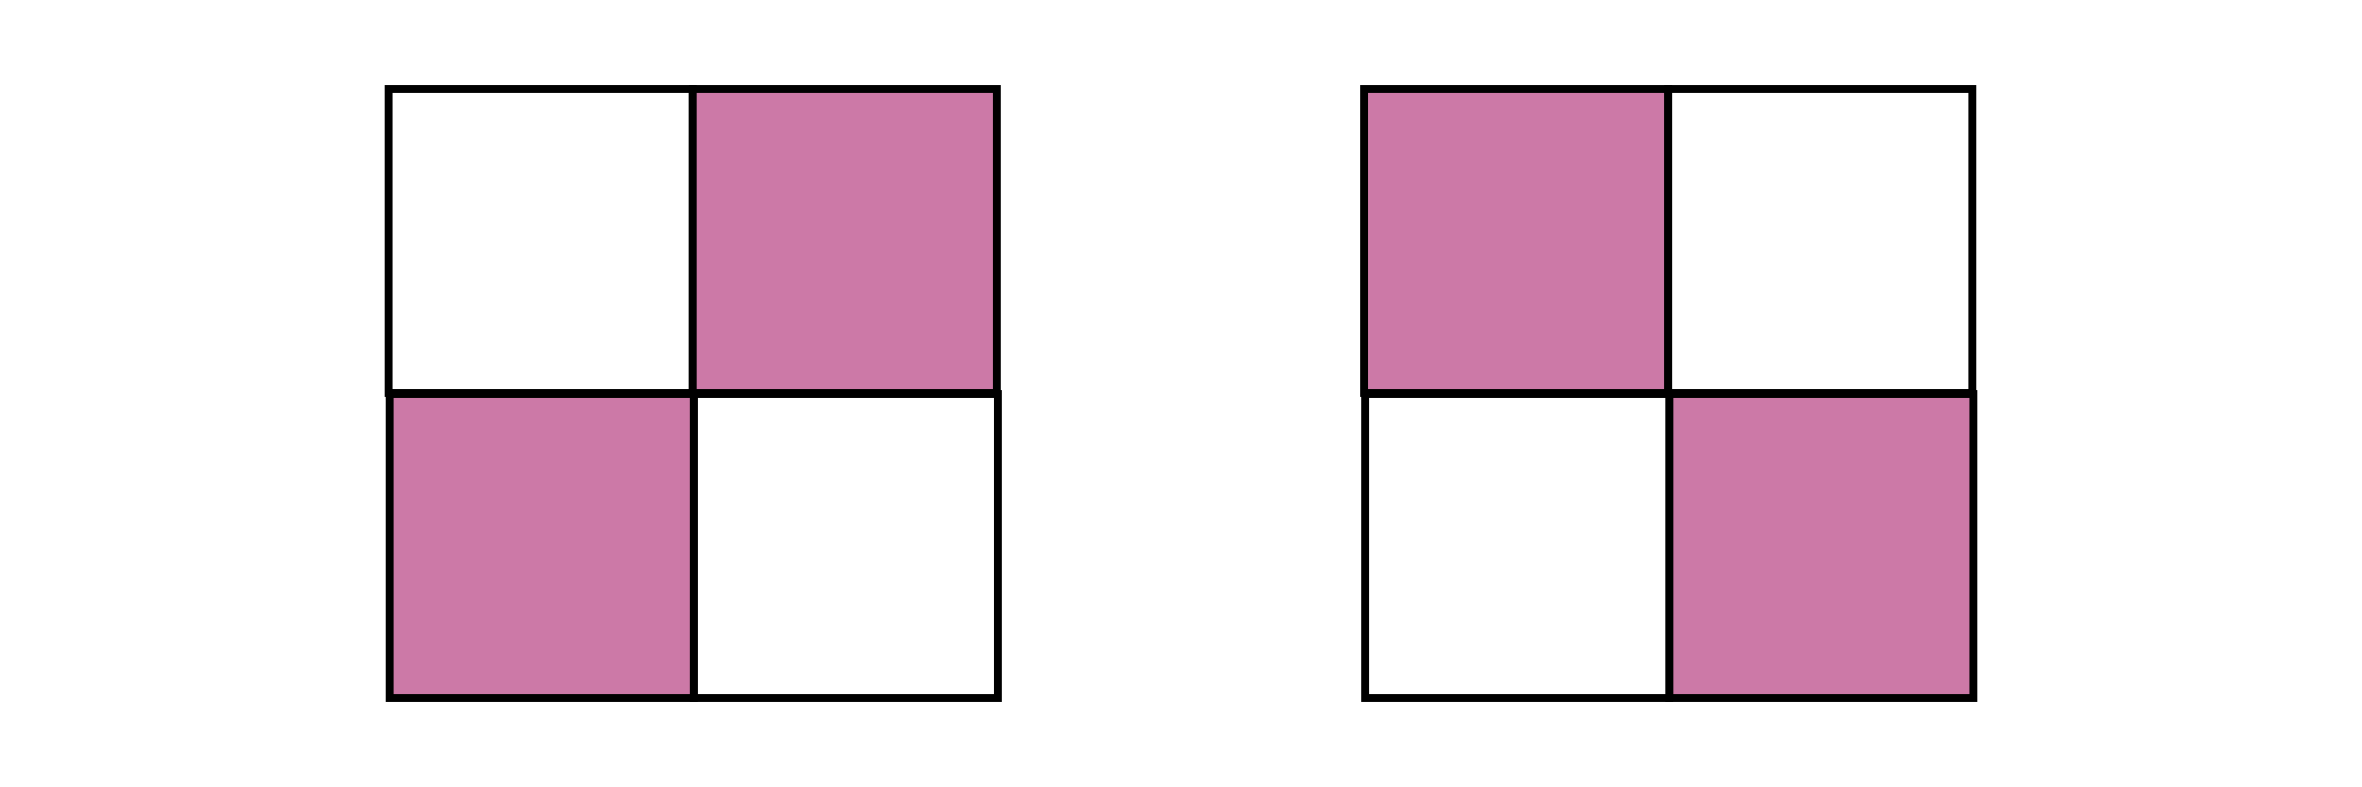
\includegraphics[width=\textwidth]{Figure 1.1.A}
\caption{A set with two states}
\end{figure}
\noindent are the collection of states that form the set $A$.

\section{Sets and Operators}
A \textbf{set}\index{set} is an non-ordered list of objects, and a single object in a set is called an \textbf{element}\index{element} of the set. Elements of a set can be numbers, words, sets in-and-of-themselves, and more. We use curly brackets \{ \} to contain elements that define a set. For example:
$$A = \{ {1,2,3,4,5,6} \}, \ B = \{ {\textnormal{``} heads \textnormal{''}, \textnormal{``}tails \textnormal{''} } \}$$
the set $A$ defines the values that a six-sided die's face may take and the set $B$ defines the state that a two-sided coin may be in. Likewise, the set:
$$C = \{ {A,B} \}$$
is a set containing the sets $A$ and $B$.

The set \textbf{union}\index{union} operator $\cup$ creates a new set that contains the elements in either of both sets. For example:
$$A \cup B = \{ {1,2,3,4,5,6, \textnormal{``} heads \textnormal{''}, \textnormal{``} tails \textnormal{''} } \}$$
is the set that contains any element in either $A$ or $B$. Note that $A \cup B$ is not the same set as $C$ because:
$$C = \{ {A,B} \} = \{ \{ {1,2,3,4,5,6} \}, \{ { \textnormal{``} heads \textnormal{''}, \textnormal{``} tails \textnormal{''} } \} \}$$
has brackets in the interior that make it a set of sets.

The set \textbf{intersection}\index{intersection} operator $\cap$ creates a new set that contains elements that are strictly in both sets. For example:
$$\{ {1,2}\} \cap \{ {2,3}\} = \{ {2} \}$$
generates a set that contains only the element $2$ because it is the only element in both sets. Note that:
$$A \cap B = \varnothing$$
states that the intersection $A \cap B$ contains no elements in common. Sets with no elements in common are called \textbf{disjoint}\index{disjoint} sets. Thus, the intersection between them is empty set $\varnothing$.

The \textbf{empty set}\index{empty set} $\varnothing$, also called the void set, is the set that contains no elements:
$$\varnothing = \{ \}$$
in which there are no elements inside the brackets. Note that $\{ \varnothing \}$ is not the same set as $\varnothing$ because the bracketing means that $\{ \varnothing \} = \{ \{ \} \}$ contains one element, the empty set.

A \textbf{tuple}\index{tuple} is an ordered list of elements. We use parentheses ( ) to contains elements that define a tuple. We may call a tuple with $2$ elements a double, $3$ elements a triple, or more generally $n$ elements an $n$-tuple. Tuples are a convenient way of batching distinct mathematical objects or elements. For example, the tuple:
$$({X, \Sigma, \mu})$$
form a tuple called a measure space.

The \textbf{set difference}\index{set difference} operator $\setminus$ creates a new set such that $L \setminus R$ is a set containing elements of the left set $L$ without elements in the right set $R$. For example:
$$\{ {1,2,3} \} \setminus \{ {2} \} = \{ {1,3} \}$$
creates a new set that only contains elements of $\{ {1,2,3} \}$ that are not in the set $\{ {2} \}$. The set difference operator $\setminus$ may also be called the without operator such that $A \setminus B$ is semantically stated as ``$A$ without $B$''.

The \textbf{symmetric difference}\index{symmetric difference} operator $\Delta$ creates a new set of elements that are not shared between both sets, or are unique to each set. For example:
$$\{ {1,2}\} \Delta \{ {2,3}\} = \{ {1,3} \}$$
is a set containing non-shared elements between $\{ {1,2}\}$ and $\{ {2,3}\}$. The symmetric difference $L \Delta R$ may also be written as:
$$L \Delta R = (L \cup R) \cap (L \cap R) = (L \setminus R) \cup (R \setminus L)$$
We may also semantically state ``the exclusives of $L$ and $R$'' or ``the uniques of $L$ and $R$'' in addition to the common phrase ``the symmetric difference of $L$ and $R$''.

The \textbf{subset}\index{subset} operator $\subseteq$ declares that all elements in the left set are elements in the right set. For example, $L \subseteq R$ declares all elements in $L$ are elements in $R$. We may say that $L$ is contained in $R$:
\begin{figure}[H]
\centering
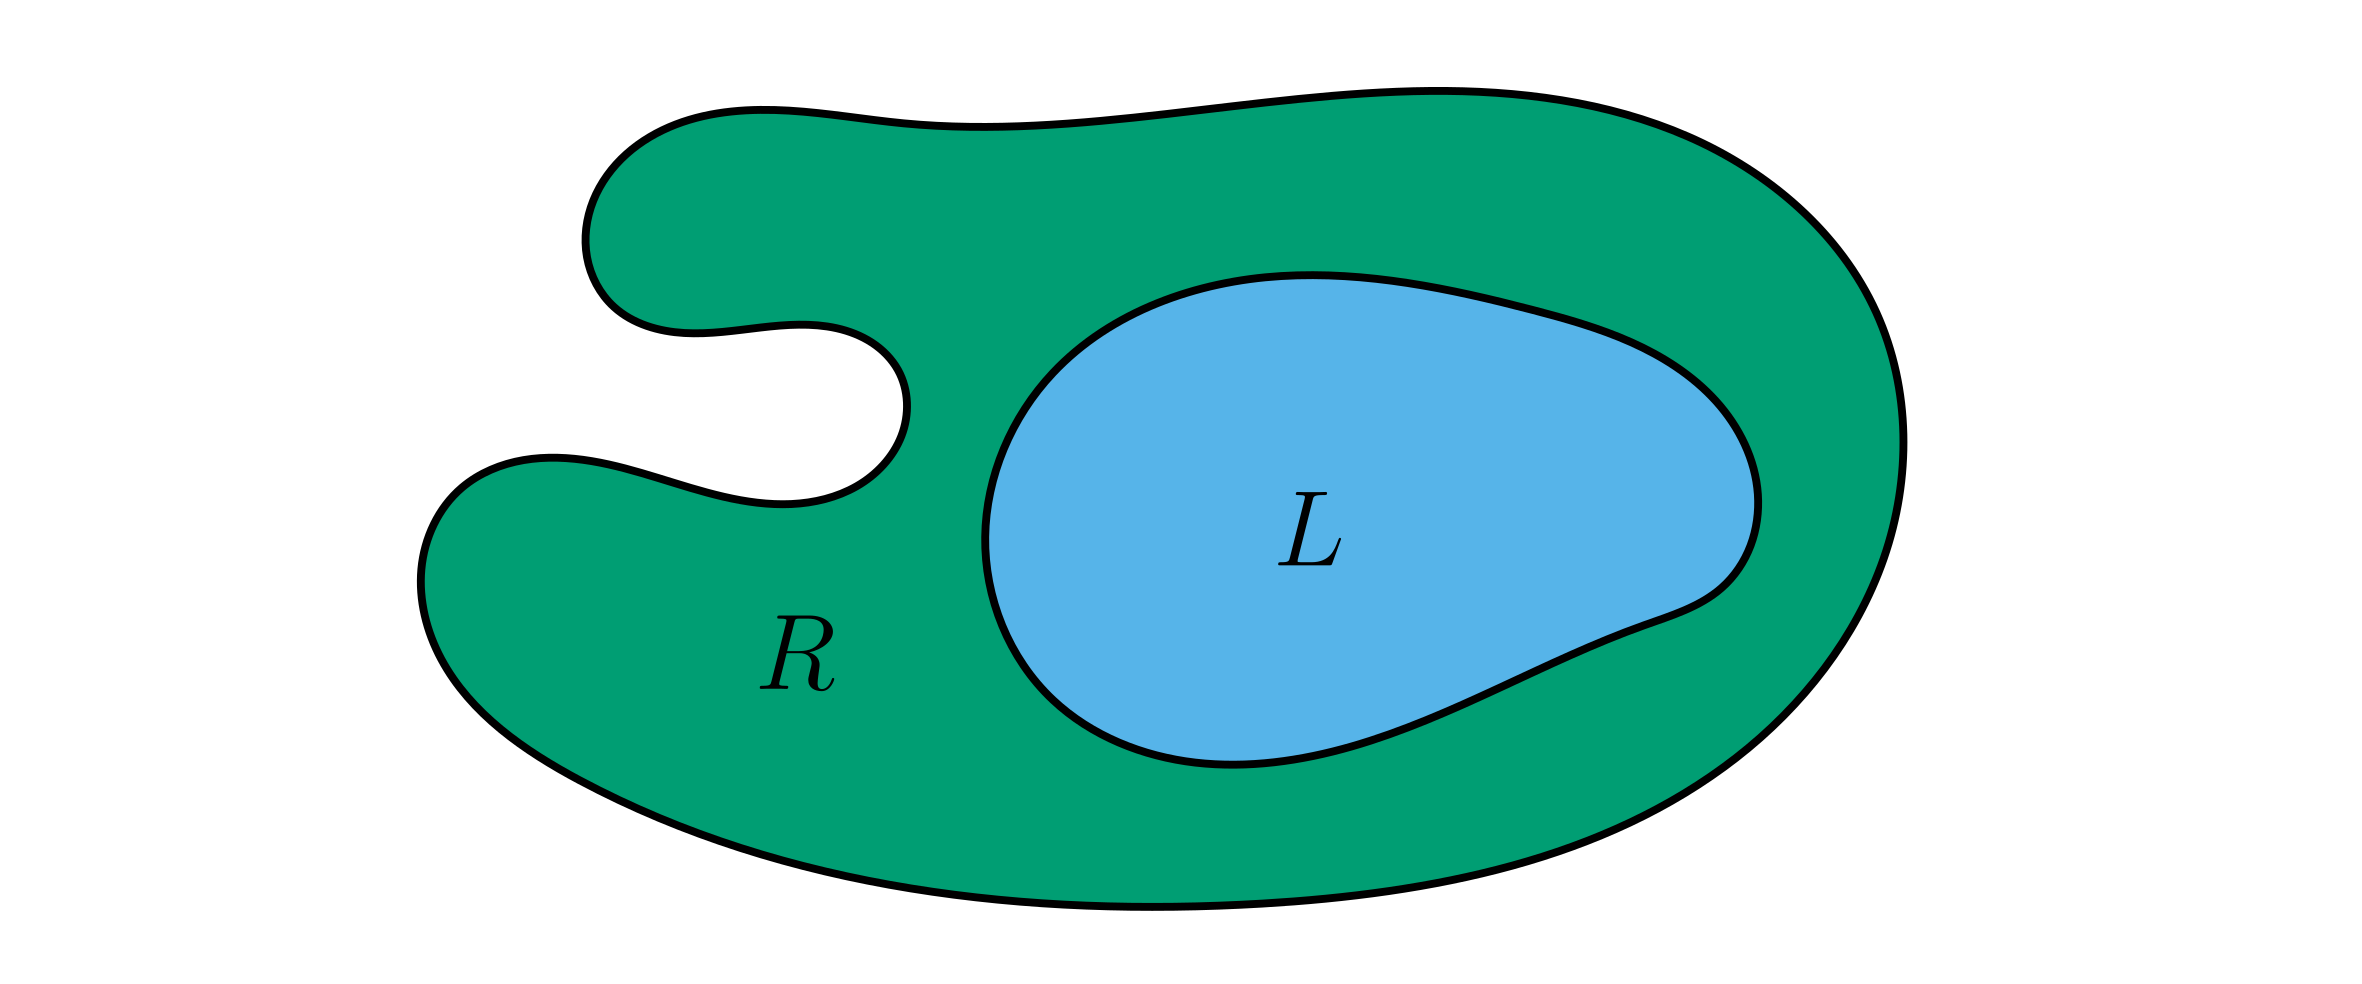
\includegraphics[width=\textwidth]{Figure 1.2.A}
\caption{The set $L$ contained in the set $R$}
\end{figure}

\noindent Note that if $L \subseteq R$ and $R \subseteq L$ are simultaneously true, then $L$ is the same set as $R$ such that $L = R$.

The \textbf{superset}\index{superset} operator $\supseteq$ declares that all elements in the left set are elements of the right set, and that the left set may contain elements outside of the right set. In this case for $L \supseteq R$, we say that $L$ contains $R$. The statement $L \supseteq R$ is the same as $R \subseteq L$.

The \textbf{proper subset}\index{proper subset} operator $\subset$ and \textbf{proper superset}\index{proper subset} operator $\supset$ are variations in which the two sets may not be equal. That is, $L \subset R$ implies that $R$ contains at least one element not in $L$.

The \textbf{element}\index{element} operator $\in$ declares that the left variable is an element of the right set. For example:
$$x \in A$$
declares that $x$ is an element of the set $A$. In this case, $x$ is a variable in which we are not specifying an exact element of $A$. If a set is an element of set $A$, then $x \in A$ means that the variable element $x$ may be a set.

The \textbf{for all}\index{for all} operator $\forall$ is used to specify all elements of a set such as the expression $\forall x \in A$. For example:
$$x < x+1, \forall x \in \{ 1,2,3,... \}$$
correctly asserts that a number is less than itself plus $1$. 

Since elements of a set are distinct from the set itself, such as $\{ \varnothing \}$ versus $\varnothing$, we use this phrase to make statements about all elements of the set rather than the set itself. It is important to distinguish this way because the proposition:
$$A \in A$$
is problematic. The statement $A \notin A$ means that $A$ is a normal set, and this is what we are normally implying when we call $A$ a set. We will discuss normal sets and set theory paradoxes in a moment.

The \textbf{there exists}\index{there exists} operator $\exists$, or the \textbf{for some}\index{for some} operator, is used to specify at least one element for a truth statement. For example:
$$x < y, \ \exists x \in \{ {0,1} \}, \ y = \{ {1} \}$$
asserts that $x$ may assume a value for which $x < y$. Since any element may fulfill the condition and at least one element does fulfill the condition, this statement is true. This is logical condition comparable to the for all operator $\forall$. For example:
$$x < y, \ \exists x \in \{ {...,-3,-2,-1} \}, \ y = \{ 1,2,3,... \}$$
is a strict condition. If there exists some $x$ that does not fulfill this condition, then the statement is not true.

This brings us to the duality of the for some operator $\exists$ and the for all operator $\forall$. If a statement is true $\forall x$, then it is not false $\exists x$. If a statement is true $\exists x$, then it is not false $\forall x$. For example:
$$x < y, \ \forall x \in \{ {0,1} \}, \ y \in \{ {1, 2} \}$$
is false because $x < y$ is false for at least one case: $x=1, y=1$. Since the proposition is false $\exists x$, then is is not true $\forall x$. We call $\neg$ the logical negation operator. We may say that for a proposition $p$ that:
$$p \ \textnormal{TRUE} \ \forall x = \neg p \ \textnormal{FALSE} \ \exists x$$
For example, if $p = x^2 > 0$ is not true for all $x$, then $\neg p$ is true for some $x$. This is based upon the assumption of the \textbf{law of the excluded middle}\index{law of the excluded middle} which claims that a statement is either true or not true, with no third option.

A \textbf{normal set}\index{normal set} is a set that does not contain itself, $A \notin A$. An \textbf{abnormal set}\index{abnormal set} is a set that contains itself $A \in A$. This brings us to Russell's paradox. Let $U$ bet the set of all objects, including itself. Let $R$ be a subset of the universal set $U$. The set $R$ is defined as the set of all sets that are not elements of themselves, or the set of all normal sets. If the Russell set $R$ is not in itself, then it is in $R$. This logical contradiction is called Russell's paradox. The Russell set $R$ therefore cannot exists. Since the universal set $U$ is a superset of $R$, then $U$ is a superset of a set that does not exists. However, $U$ contains $R$ as an element. Therefore, the set of all sets $U$ does not exist.\footnote{The contradiction lies in the fact that we know that normal sets exist.}

A simpler proof that the set of all sets $U$ does not exists uses the power set function. The \textbf{power set}\index{power set} of $A$, $\mathcal P (A) = 2^A$, is the set of all subsets of $A$. The convention $2^A$ is a notation in which each element in $A$ may be assigned an element from the set $\{ {0, 1} \}$, a binary set in which $1$ means in the subset and $0$ means not in the subset. Let $2^U$ be the power set of the set of all sets. The size of the power set of $A$ is bigger than $A$ for any set, except the empty set. However, $2^U$ must be a proper subset of $U$. We cannot have $U \subset 2^U$ and $2^U \subset U$ simultaneously. Therefore, the set of all sets $U$ does not exist.


We will discuss more about cardinality, or the size of a set, in section 1.4: Cardinality and Infinite Cardinals.
\section{Measures and Mappings}
A \textbf{map}\index{map} or \textbf{mapping}\index{mapping} is a function $f$ that sends elements from a set $X$ to a set $Y$. We therefore call the set $X$ the \textbf{domain}\index{domain} of the function $f$ and call the set $Y$ the \textbf{codomain}\index{codomain} of the function $f$. The \textbf{image}\index{image} of a function $f$, denoted $f(X)$, is the subset of $Y$ that may originate from the mapping function $f$ upon elements of $X$, $x \in X$. The image of an element $x$ is stated as $f(x)$, and $f(x) \in f(X) \subset Y$.

\begin{figure}[H]
\centering
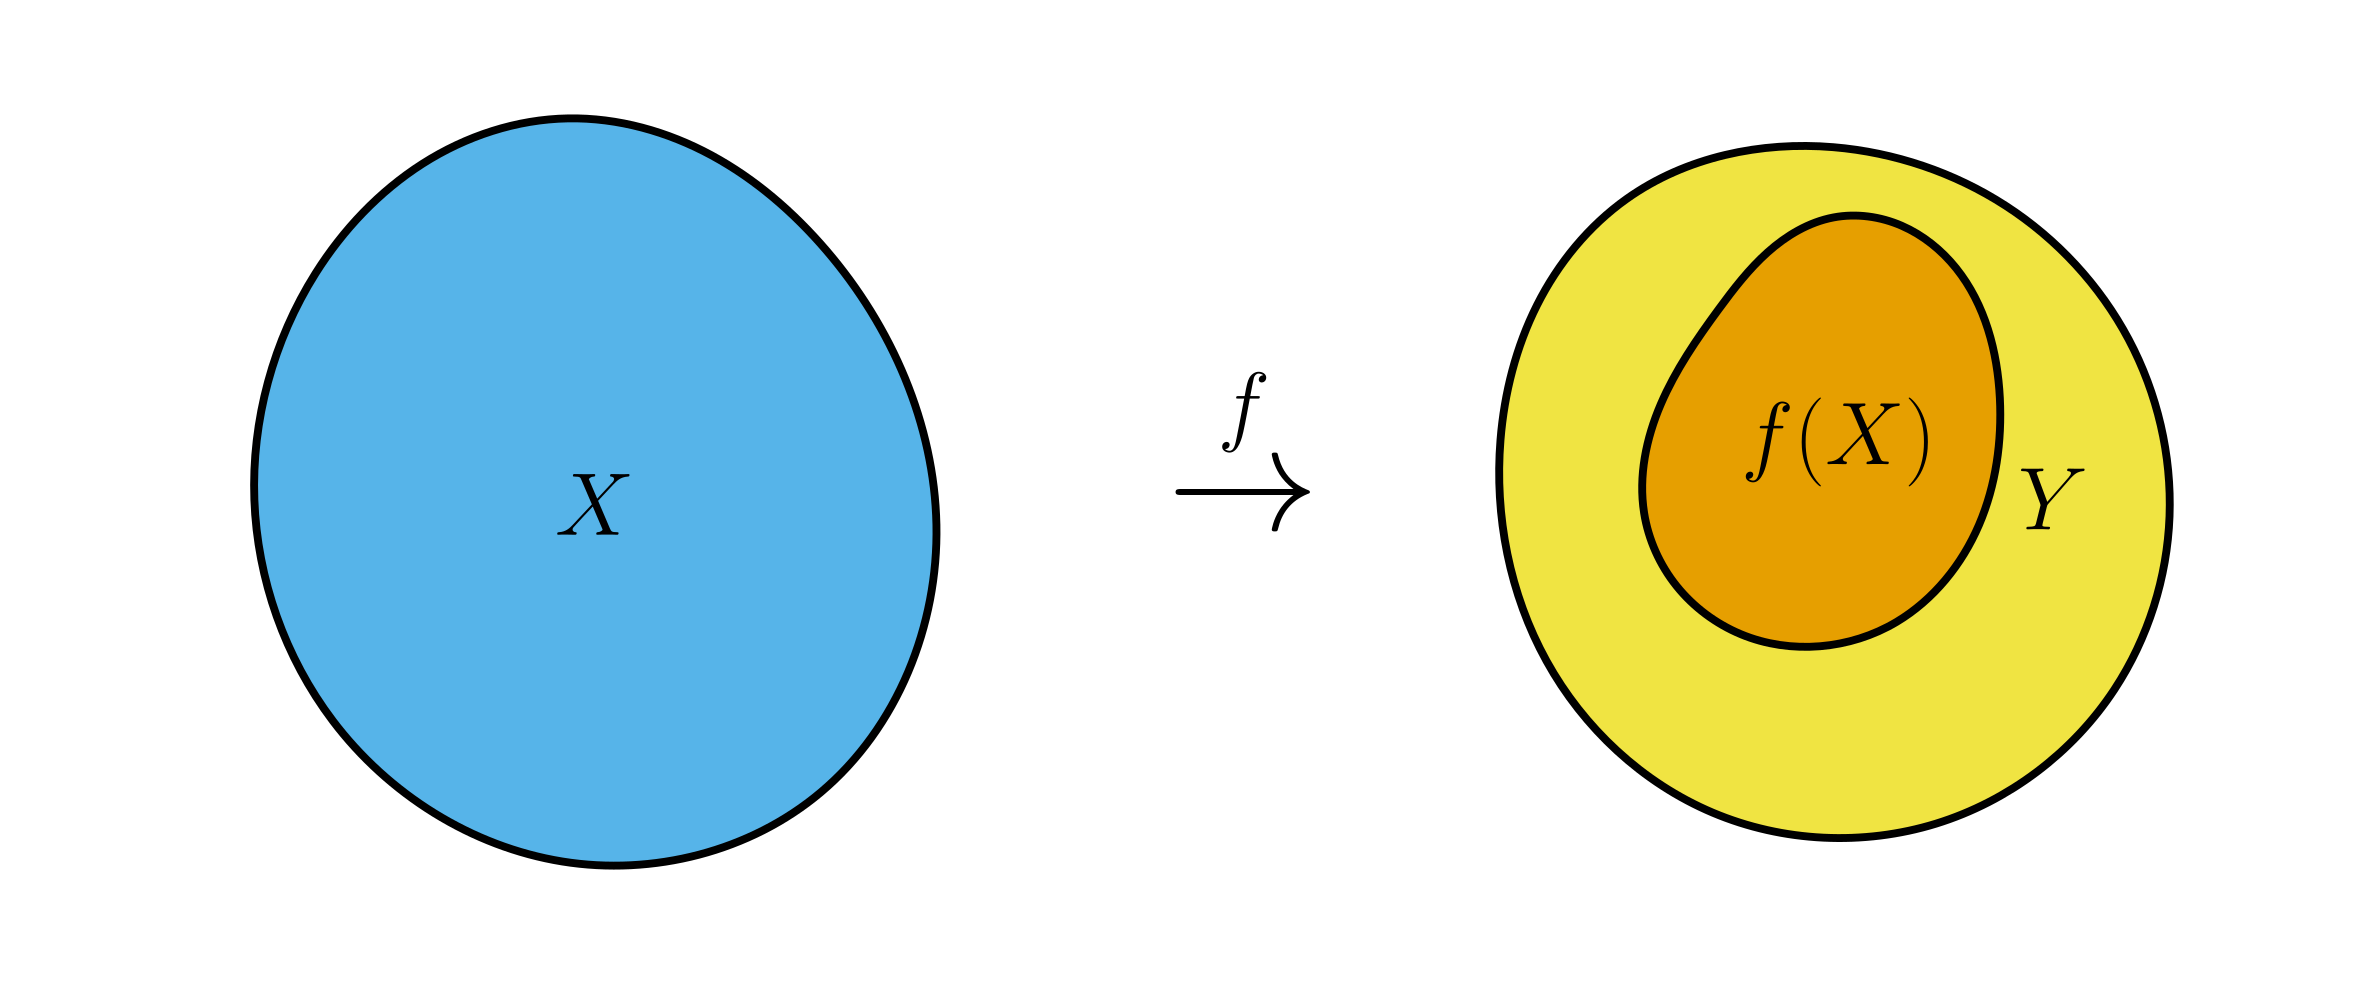
\includegraphics[width=\textwidth]{Figure 1.3.A}
\caption{The mapping $f$ of $X$ to the part of $Y$ denoted $f(X)$}
\end{figure}
\noindent The image set $f(X)$ may also be called the output space of the input space $X$.

A good rationale for distinguishing between $f(X)$ and $Y$ is for a restricted input domain. If we define $X$ to be the integers $\mathbb Z$, $Y$ to be the real numbers $\mathbb R$, and $f$ to be a function $f(x) = x^2$, then our image set $f(X)$ is only a countably finite subset of $Y$. Even though the function $f(x)$ is well-defined if we decide upon $X$ as the real numbers $\mathbb R$, our choice of domain restricts the image.

A function $f$ is considered \textbf{bijective}\index{bijective} if it is both injective and surjective. The function $f$ is called \textbf{injective}\index{injective} if each element $y \in Y$ receives at most one element $x \in X$. The function $f$ is called \textbf{surjective}\index{surjective} if each element $y \in Y$ receives at least one element $x \in X$. Probability functions are not necessarily injective or surjective.

\begin{figure}[H]
\centering
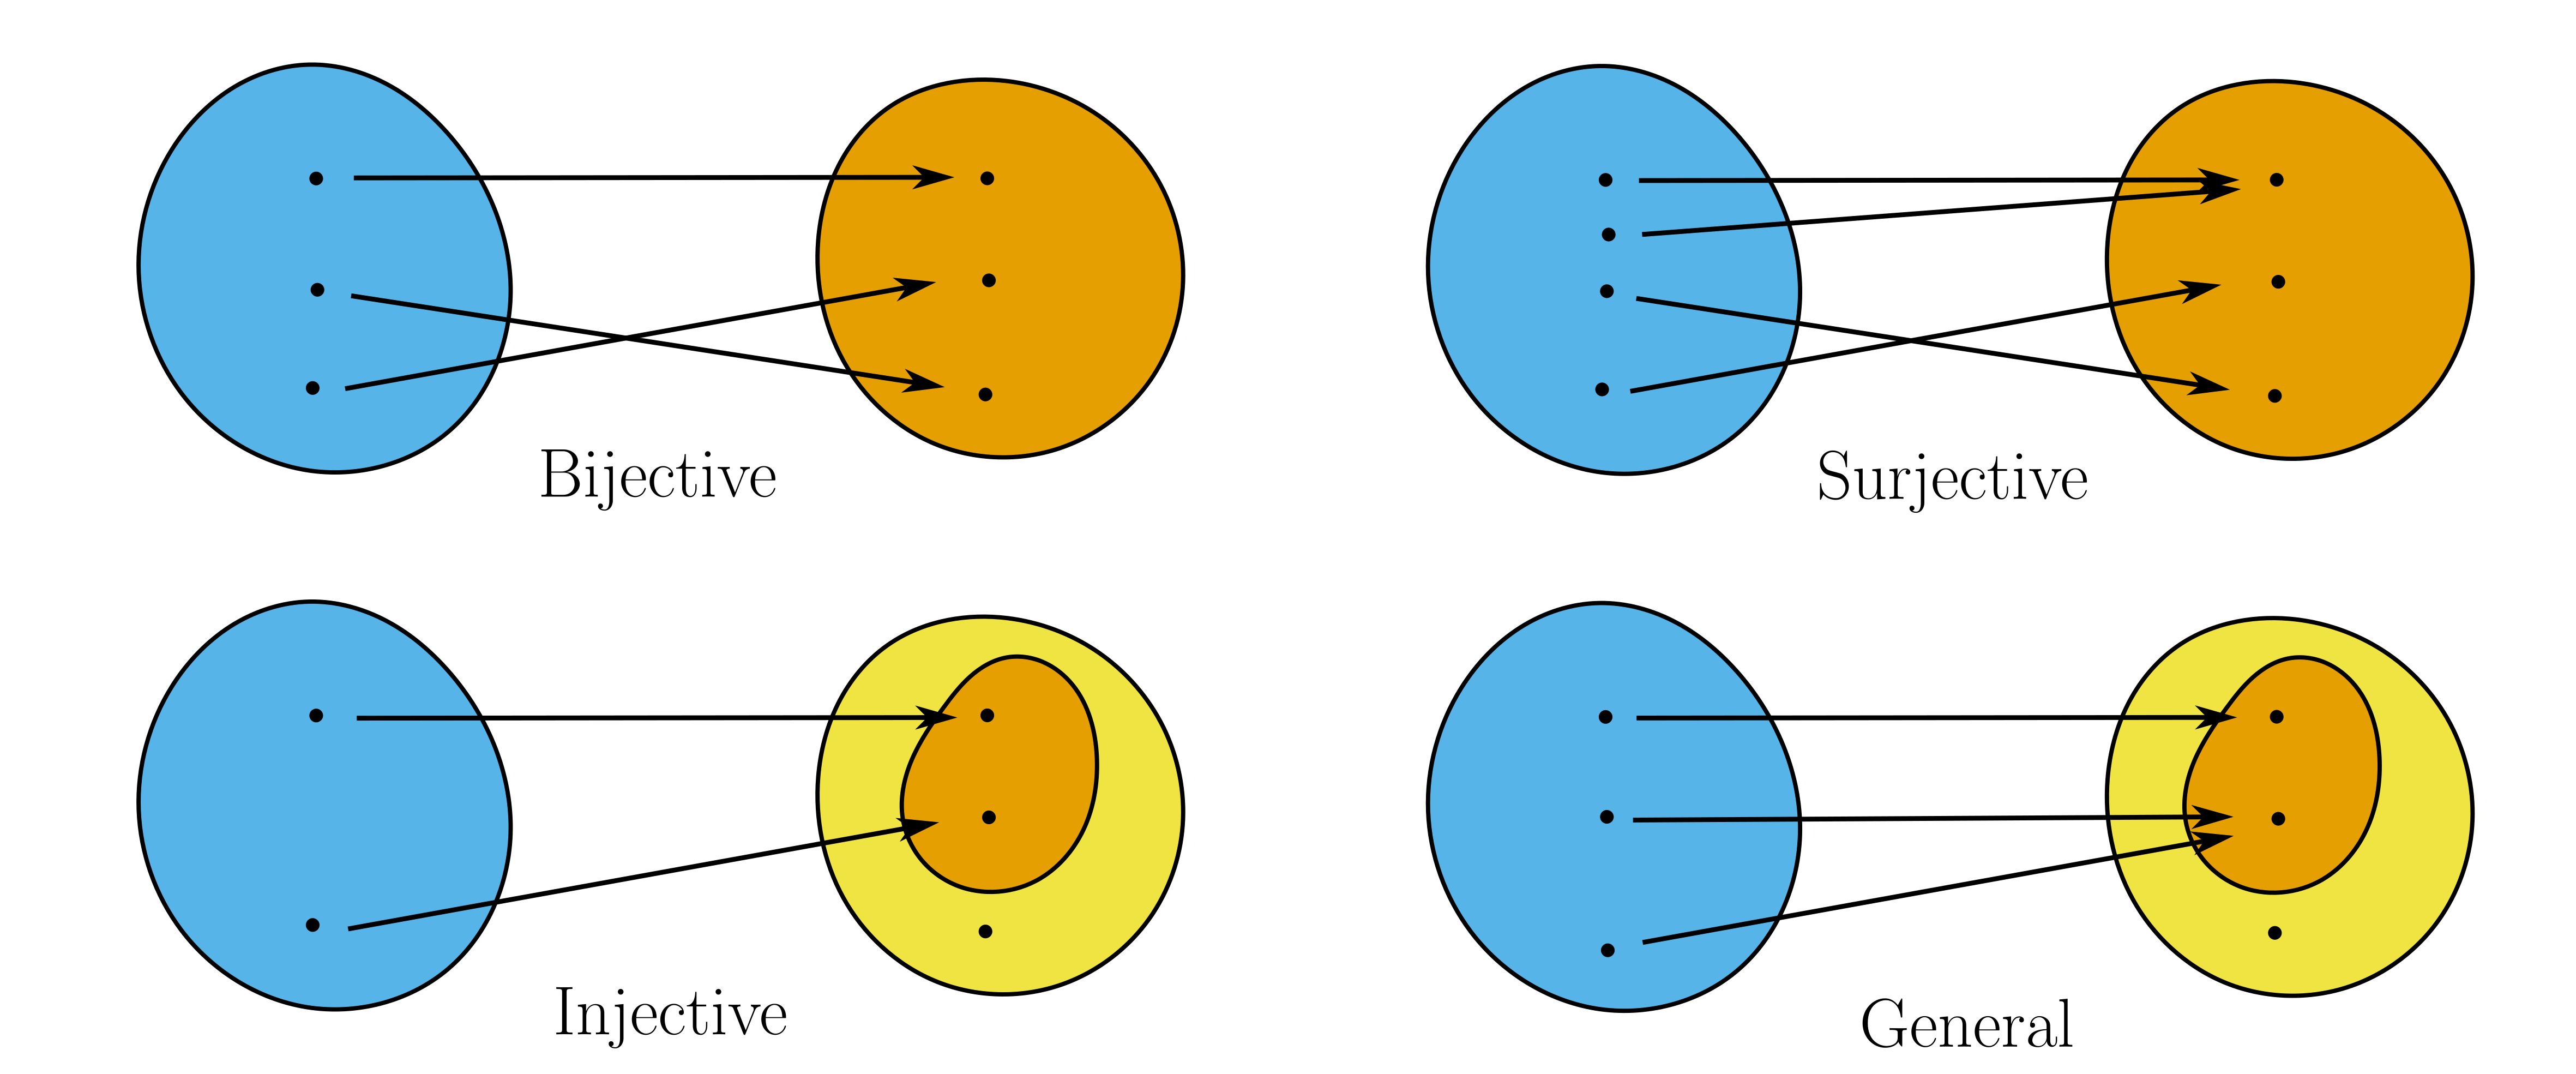
\includegraphics[width=\textwidth]{Figure 1.3.B}
\caption{Comparison of bijective, surjective, injective, and general functions}
\end{figure}

A set function $\mu$ acting on a set $X$ and its $\sigma$-algebra $\Sigma$ must fulfill these key properties as a mapping in order to be called \textbf{measure}\index{measure}:
\begin{enumerate}
\item $\mu ( \varnothing ) = 0$
\item $\mu ( E ) \ge 0, \ \forall E \in \Sigma$
\item $\mu \big ( \bigcup\limits_{i=1}^n E_i \big ) = \sum\limits_{i=1}^n \mu( E_i ) \ \textnormal{ for disjoint sets } \ E_i$
\end{enumerate}
The double $( X, \Sigma )$ is called a \textbf{measurable space}\index{measurable space} and the triple $(X, \Sigma, \mu)$ is called a \textbf{measure space}\index{measure space}. This is the logic in formal science that matches our intuition of measurement in the natural sciences and real-life.

A \textbf{$\boldsymbol \sigma$-algebra}\index{sigma algebra} of $X$, $\Sigma$, is a subset of the power set of $X$, $\mathcal P (X) = 2^X$, with the following properties:
\begin{enumerate}
\item $E_i \in \Sigma, \forall E \in \Sigma, E^c_i = X \setminus E$
\item $E_i \cup E_j \in \Sigma, \forall E_i, E_j \in \Sigma$
\item $E_i \cap E_j \in \Sigma, \forall E_i, E_j \in \Sigma$
\end{enumerate}
These properties are called \textit{closure under complementation}, \textit{closure under union}, and \textit{closure under intersection}. \textbf{Closure} means that the operation on elements of the set $\Sigma$ produces elements of the set $\Sigma$. The \textbf{complement}\index{complement} of $E$ is called $E^c$, and the complement is only defined for $E \subseteq X$ in which X may be called the \textbf{universe set}\index{universe set} of $E$. Since $E^c = X \setminus E$, then:
$$E^c \cap E = \varnothing$$
This means that the complementary subsets $\{ E, E^c \}$ of the universe set $X$ are disjoint. Since $X$ and $X^c$ are complements, their union:
$$E^c \cup E = X$$
should return the universe set $X$. The universe set $X$ is the set of all objects under consideration, and it is a normal set such that $X \notin X$. It is with universe sets and complements that we may now define partitions of $X$. 

Let us denote the subsets of $X$ as $P_1, P_2, ... P_n$, and they are called \textbf{partitions}\index{partition} of $X$ if for $A = \{1,...,n\}$:
\begin{enumerate}
\item $P_i \cap P_j = \varnothing; \ i \neq j; \ i,j \in A$
\item $P_i \cap P_i^c= \varnothing; \ P_i^c = \bigcup\limits_{j \in A \setminus i} P_j$
\item $P_i \neq \varnothing; \ \forall i \in A$
\item $\bigcup\limits_{i \in A} P_i = X$
\end{enumerate}
The first defines partitions of $X$ are mutually disjoint sets of X. The second property defines the complement of any partition is the union of the other partitions. The third property defines that any partition may not be the empty set. The fourth property defines that the union of all partitions must cover $X$ in order to be equal to the universe set $X$ in order to be a complete set of partitions. If $P_i \in X$, then $P_i$ is said to be an \textbf{elemental partition}\index{elemental partition}, or a singular partition\index{singular partition}, of $X$. An example of partitions of the set $X = \{ 1,2,3,4 \}$ is:
$$P_1 = \{1\}, \ P_2 = \{2\}, \ P_3 = \{3,4\}$$
A $\sigma$-algebra of $X$, denoted $\Sigma$ is not just any subset of $2^X$. It must be the binary inclusion or exclusion of partitions $P_1,...,P_n$ of $X$. Therefore, the size of the set $\Sigma$ must therefore be $2^n$ in which $n$ is a natural number $\mathbb N$.

\begin{figure}[H]
\centering
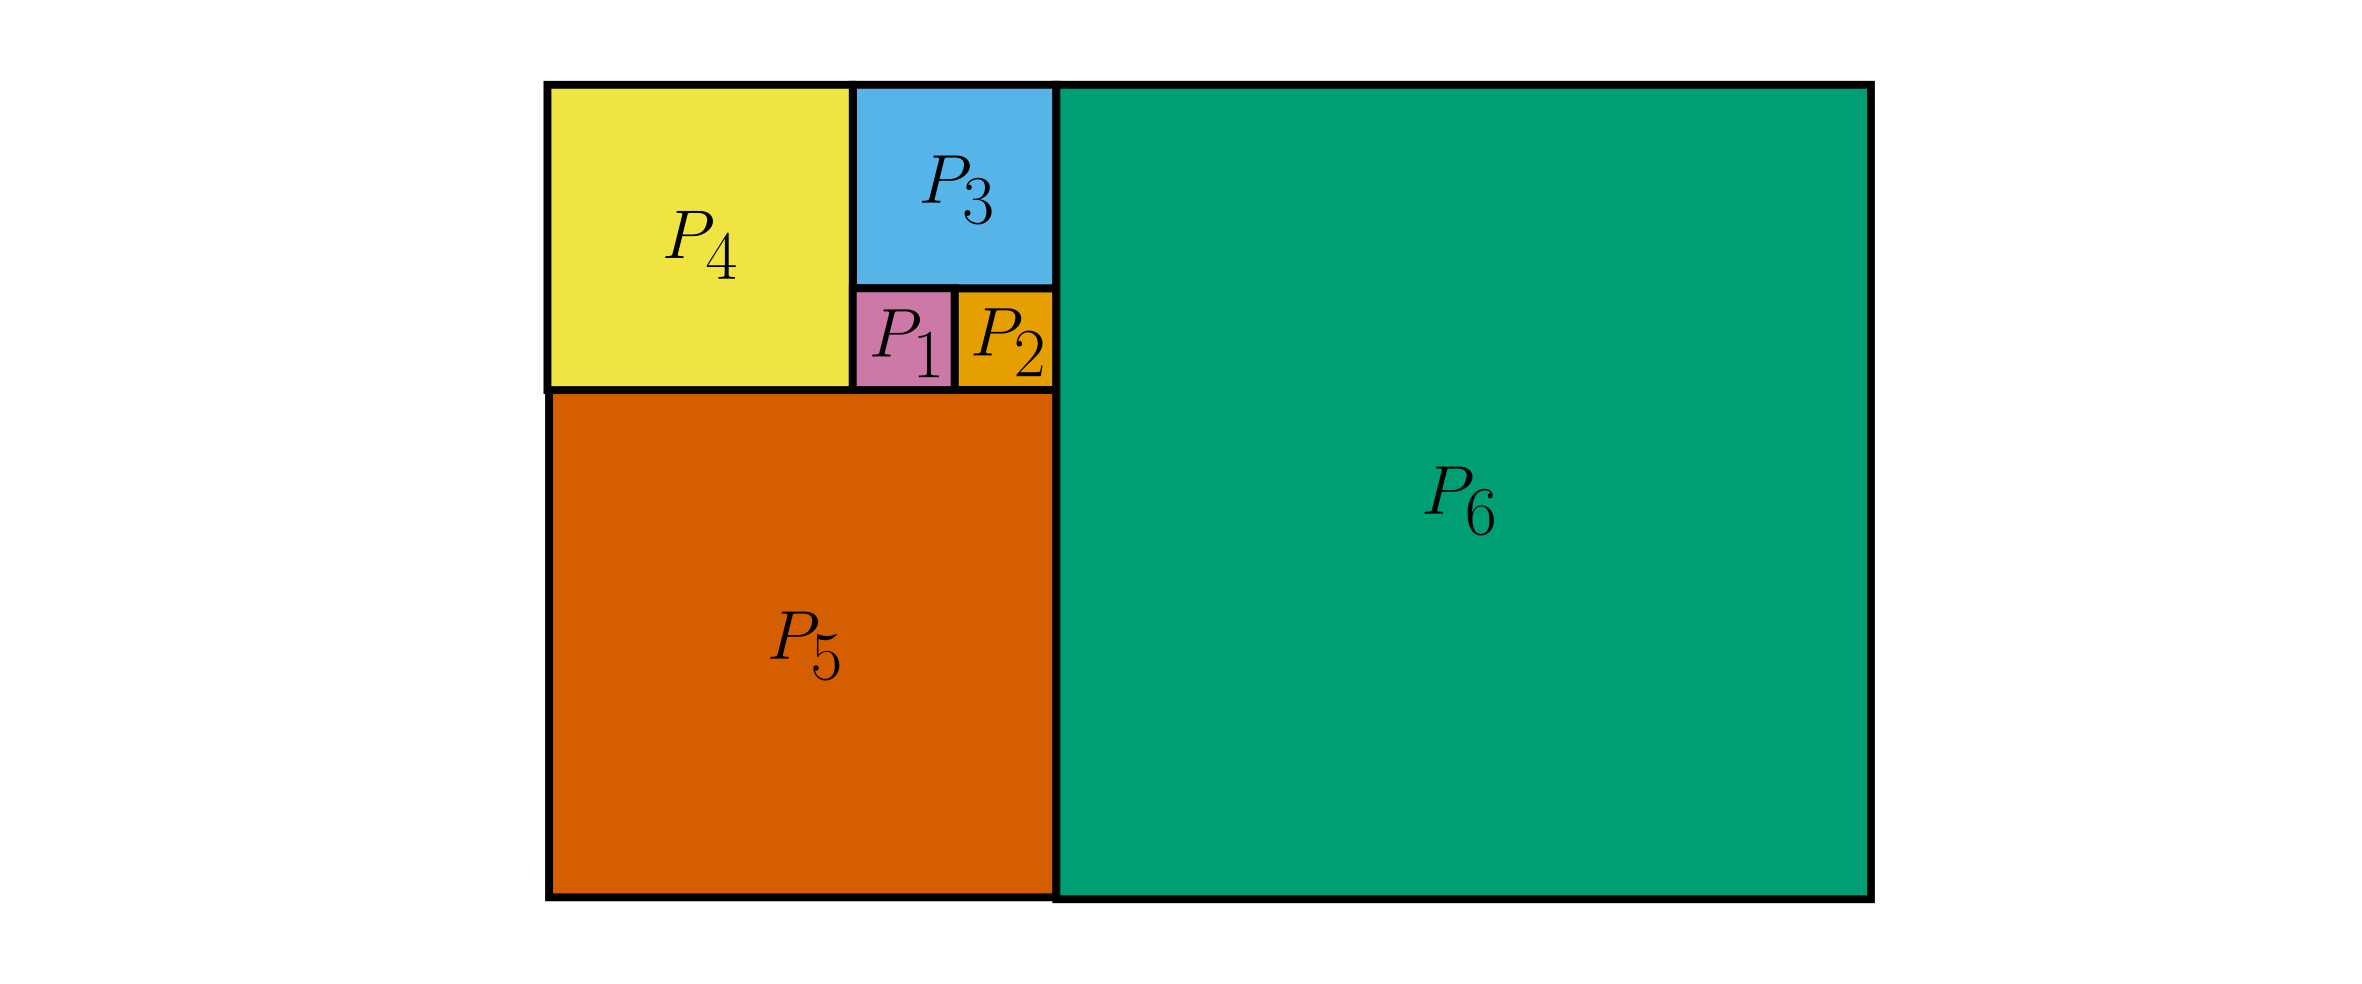
\includegraphics[width=\textwidth]{Figure 1.3.C}
\caption{A $\sigma$-algebra's elements are partitions that must be included or excluded}
\end{figure}

\section{Cardinality and Infinite Cardinals}
The \textbf{cardinality}\index{cardinality} of a set $X$, denoted as $\textnormal{card}(X)$ or $|X|$, is a measure of the number of elements in the set $X$. For a finitely countable set, the cardinality is an element of the set of natural numbers $\mathbb N = \{0,1,2,...\}$. For example, the cardinalities of some finite sets are given below:
$$|\varnothing| = 0, \quad |\{ 1,2,4,8,16\}| = 5$$
When we define the power set of a set $X$, the size of a its power set is $2^{|X|}$. For example, the cardinality of $2^{|\varnothing|} = 2^0 = 1$.

As a side note, we may generalize the definition power sets via \textbf{set exponentiation}\index{set exponentiation} using other integers such as $3^A$ or $4^A$. Interpret the power set $2^A$ as generating all possible combinations of assigning two colors to the set $A$ such as $\{ \textnormal{black}, \textnormal{white} \}$. We may likewise interpret $3^A$ as generating all possible combinations of assigning three colors to the set $A$ such as $\{ \textnormal{red}, \textnormal{green}, \textnormal{blue} \}$. We define:
$$Y^X$$
as the \textit{set of all functions} from $X$ to $Y$. If there are $|Y|$ categories to assign elements of $X$ into, then there are a total of $|Y|^{|X|}$ unique functions.

The cardinality of infinite sets is another matter. Any set $X$ with the same cardinality as the set of natural numbers $\mathbb N$ is said to be countably infinite. The cardinality of the set of natural numbers is given by the \textbf{transfinite cardinal number}:
$$|\mathbb N| = \aleph_0$$
in which $\aleph$ is the Hebrew letter known as aleph. Other sets with the cardinality aleph-zero (also called aleph-null) are the set of integers $\mathbb Z = \{ ...-2,-1, 0, 1,2...\}$, the set of even integers $\{ ...,-2,0,2,...\}$, and the set of integer powers of 2 $\{ ...,2^{-1}, 2^0, 2^1,...\}$.


The cardinality of the set of real numbers $\mathbb R$ is aleph-one $\aleph_1$. Any set $X$ that has the same cardinality as the real numbers has $\aleph_1$ has a cardinality greater than aleph-zero, $|X| = \aleph_1 > \aleph_0$. Both sets $\mathbb R$ and $\mathbb Z$ are infinite sets, but the real numbers $\mathbb R$ is called uncountably infinite while the natural numbers $\mathbb Z$ is countably infinite. This brings us to the question about the statement relating $\aleph_0$ and $\aleph_1$:
$$2^{\aleph_0} = \aleph_1$$
This statement is called the \textbf{continuum hypothesis}\index{continuum hypothesis}, and it cannot be proven or disproven as necessarily true within the axioms of set theory. If you assume the \textbf{axiom of constructibility}\index{axiom of constructibility}, or that all sets can be described or constructed using simpler sets, then the \textbf{general continuum hypothesis}\index{generalized continuum hypothesis} is true:
$$2^{\aleph_n} = \aleph_{n+1}$$
We define $\aleph_{n}$ as the $n$-th \textbf{aleph number}\index{aleph number}.

The axiom of constructibility is akin to how a binary computer may represent computable objects. Constructive mathematics is strict in the sense that a mathematical object exists if you can construct it. If we are assuming the common Zermelo–Fraenkel axioms, assuming the axiom of constructibility also implies a few other things such as axiom of choice. This strictness makes constructive mathematics and axiom of constructibility unpopular frameworks to prove statements in.

The binary computers of today essentially rely on the assumption that $2^{\aleph_0} = \aleph 1$ and theories of computing convergence in order to make calculations of continuous objects such as gravity, electromagnetics, and computer-aided design (CAD). There are many interesting mathematical objects in statistics that emerge as a result of discrete probability relating to continuous probability in some limiting cases, such as the Normal distribution and central limit theorem. Without the assumption of continuum hypothesis or the much stronger axiom of constructibility, it is naive to assume that computers are capable of accurately modeling real-life phenomena.

\chapter{Statistical Inference}
\section{Motivations for Learning Statistical Inference}
\textbf{Statistics}\index{statistics} is the branch of mathematics that deals with extracting knowledge from uncertain events. Many of the most interesting phenomena of the natural world can only be measured and understood via probability, like a game of chance. At a fundamental level, the physics of quarks and their compositions, known as hadrons, behave precisely according to the axioms of probability. Without statistical inference, the modeling of random objects becomes impossible to us.

There is much philosophy to be debated about a random universe. If our brains are merely particles bumbling about, do we truly make choices with free will at all? Statistics says not.

For Boolean mechanics, statistical inference is important for when we define the properties of individual particles, entire systems of particles, and how much information that a system may represent. For example, the following simple random walk simulation with reflecting wall:
\begin{figure}[H]
\centering
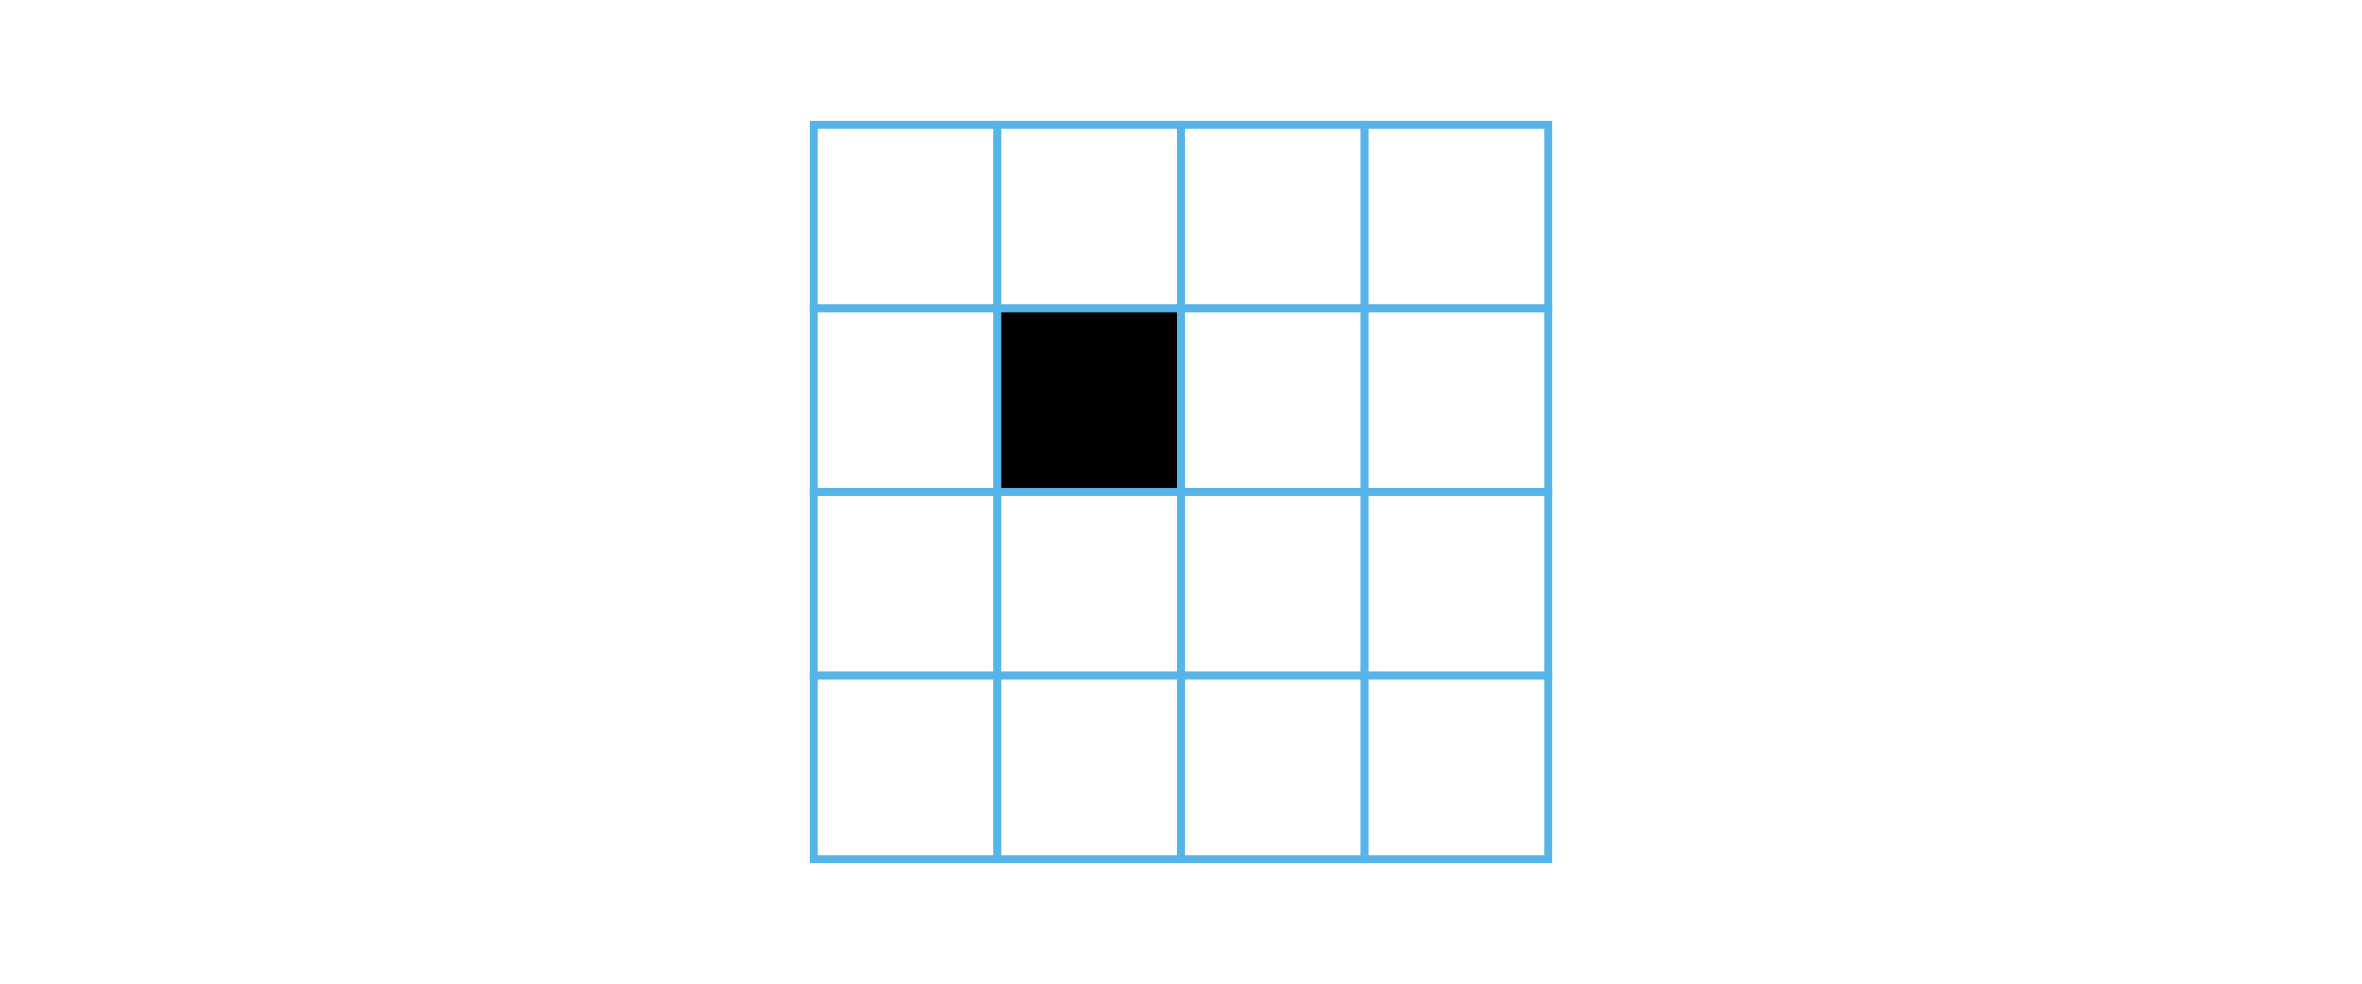
\includegraphics[width=\textwidth]{Figure 2.1.A}
\caption{A lone random walker bound to a $4 \times 4$ grid}
\end{figure}
\noindent
has a single particle and $15$ antiparticles. The lone particle will have an average position of $(2.5, 2.5)$, yet it may never actually occupy that position. It may only have a realized $x_1$-coordinate from $\{1,2,3,4\}$ and $x_2$-coordinate from $\{1,2,3,4\}$.

Another Boolean mechanics example involves two particles in an infinite antiparticle sea, or two random walkers on an infinite grid, at time $t=0$:

\begin{figure}[H]
\centering
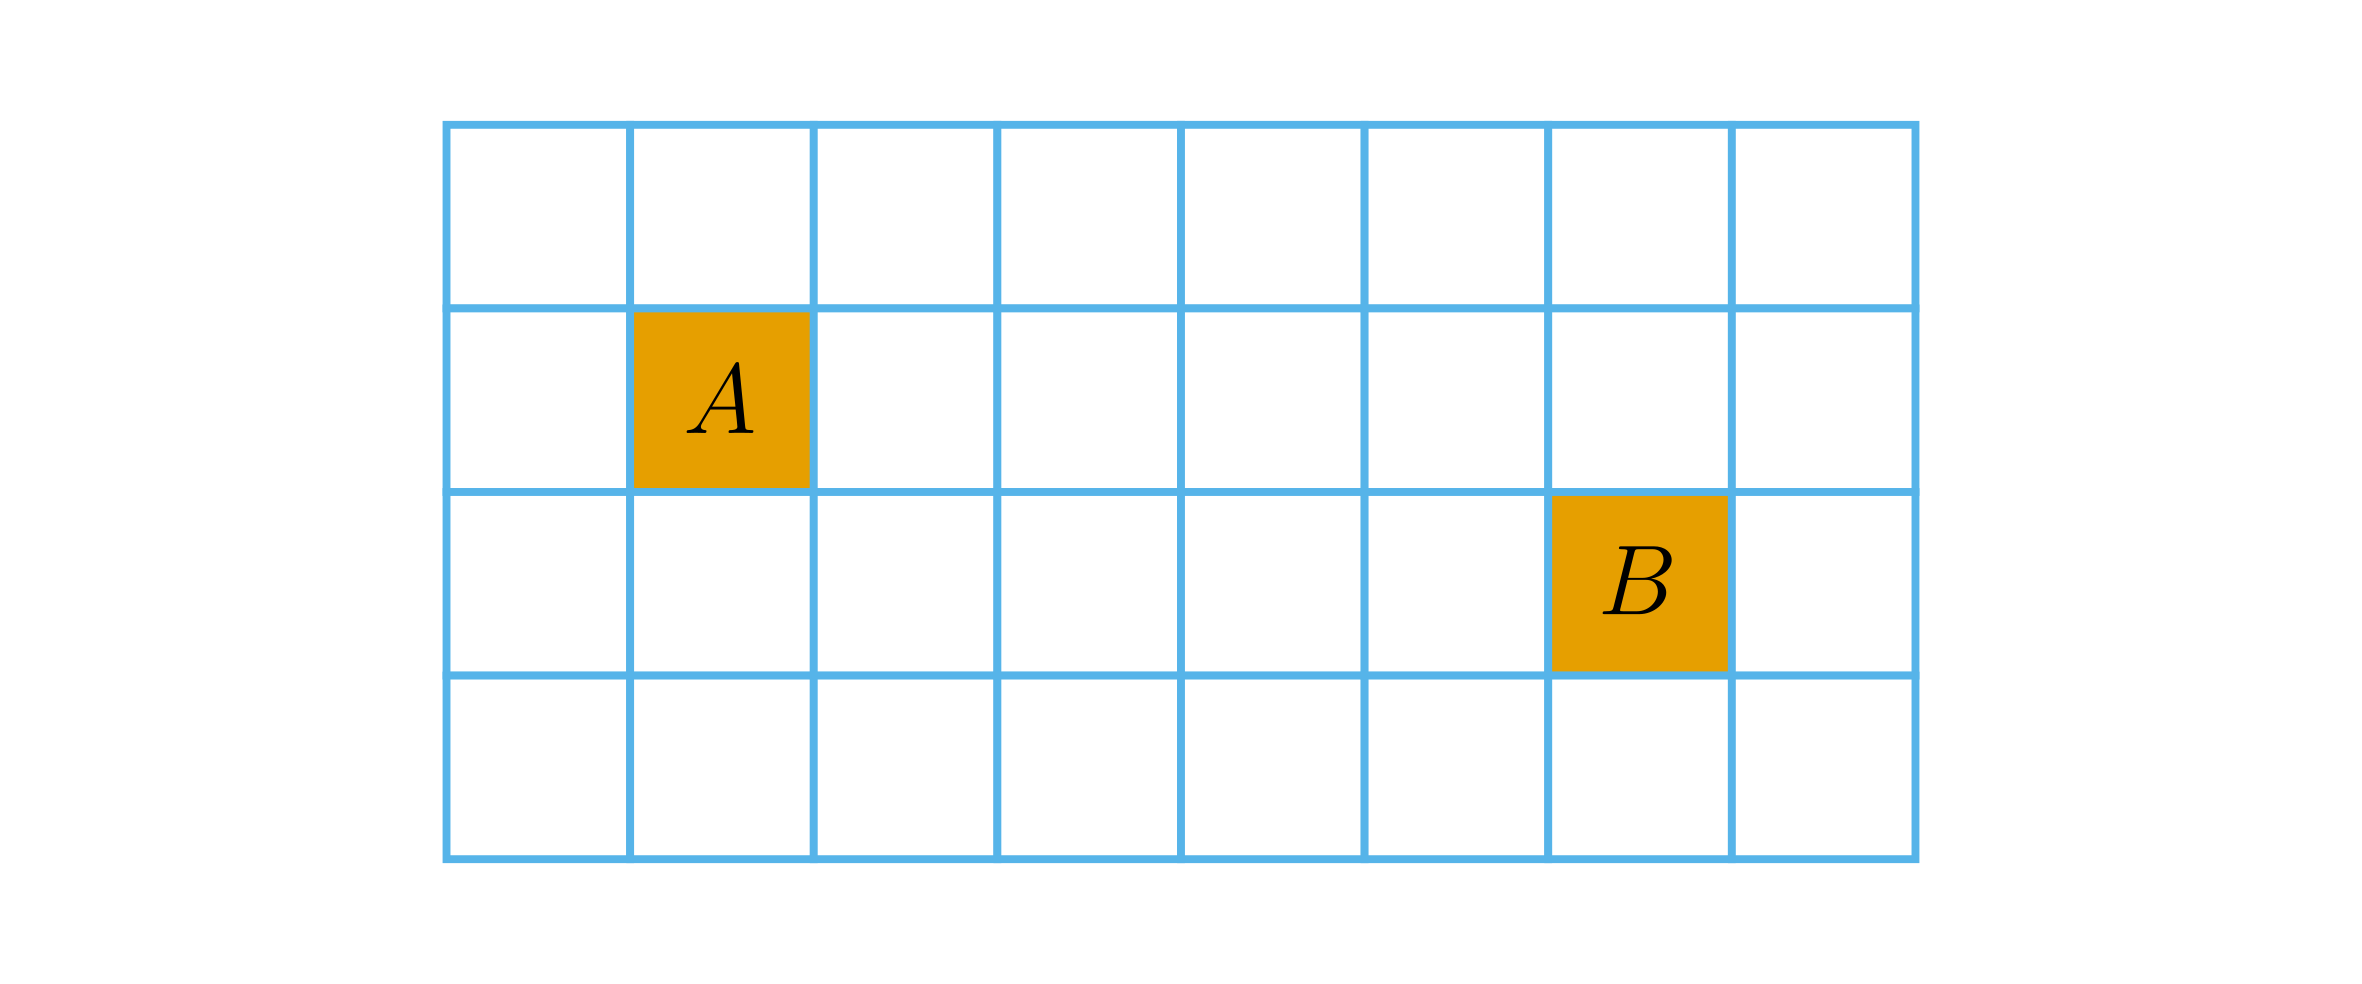
\includegraphics[width=\textwidth]{Figure 2.1.B}
\caption{A random walker $A$ influencing the probability of random walker $B$ at some unknown future time step}
\end{figure}

\noindent What can we measure about the position of the particles in the future? The average position of the particles in the future is where they are at $t=0$ until they have a probability of collision. From there, the average position of each particle shifts. The variance, or uncertainty of position, of the position of each particle in the future increases over time. The entropy, or uncertainty of information, of each particle's position also increases over time. What is the best way to measure uncertainty and why?

\section{Kolmogorov's Axioms of Probability}
The \textbf{axioms of probability}\index{axioms of probability} define a relation upon a measure space $(X, \Sigma, P)$ in which $X$ is a set, $\Sigma$ is a $\sigma$-algebra of $X$, and $P$ is a probability measure on any set of events $E \in \Sigma$. These relations are as follows:
\begin{enumerate}
\item $P(E) \in \mathbb R; \ P(E) \geq 0, \ E \in \Sigma$
\item $P(X) = 1, \ P(\varnothing) = 0$
\item $P \big ( \bigcup\limits_{i=1}^n E_i \big ) = \sum\limits_{i=1}^n P( E_i ) \ \textnormal{for disjoint sets} \ E_1, ..., E_n$
\end{enumerate}
These simple rules form the basis of all study and knowledge in probability and statistics, and they are known as Kolmogorov's axioms of probability. This set of axioms is so prevalent that it is simply referred to as the axioms of probability.

The first axiom is the \textbf{law of some probability}\index{law of some probability}, and it states that the probability that $x \in E$ is some real number greater than or equal to 0:
$$P(x \in E) \geq 0$$
Note that $E$ is an element of $\Sigma$, the $\sigma$-algebra of $X$. If $X$ has cardinality $|X| = n$, then the largest possible $\Sigma$ has cardinality $|\Sigma| = 2^n$. We may have a smaller cardinality of $|\Sigma| = 2^m$ if we assign $n$ elements to $m$ classes. For example, the largest $\sigma$-algebra of $X = \{0, 1\}$ is:
$$\Sigma = \{ \{\}, \{0\}, \{1\}, \{0, 1\}\}$$
By assigning $n$ elements to $m$ classes, it may be reduced to:
$$\Sigma = \{ \{\}, \{0, 1\}\}$$
In general, the set of all functions $m^n$ defines all these possible merges for a total of $|m|^{|n|}$ ways to create a smaller $\sigma$-algebra.

The second axiom is the \textbf{law of total probability}\index{law of total probability}, and it states that the probability that a specific event $x$ is from $X$ equals $1$:
$$P(x \in X) = 1$$
It also states conversely that the probability that the probability that a specific event $x$ has not measure is impossible:
$$P(x \in \varnothing) = 0$$
but that is already implied by the definition of a measure space. In simple terms, the probability of an event is between $[0,1]$, the probability of any event is $1$, and the probability of no event is $0$.

The third axiom is the \textbf{law of additive probability}\index{law of additive probability}, and it states that the probability measure of an aggregation of disjoint sets equals the sum of probability measure of each disjoint set. For example, the probability of a dice roll is given by the set $\{1, 2, 3, 4, 5, 6\}$.
The probability of rolling a $1$ is given by:
$$P(x \in {1}) = \frac{1}{6}$$
Likewise the probability of rolling a $2$ is given by:
$$P(x \in {2}) = \frac{1}{6}$$
The probability of rolling from the set $\{1, 2\}$ is additive:
$$P(x \in {1, 2}) = P(x \in {1}) + P(x \in {2}) = \frac{1}{6} + \frac{1}{6} = \frac{2}{6}$$
As long as events are disjoint, their total probabilities are additive.

The strictness and simplicity of Andrey Kolmogorov's axioms allow us to analyze and understand probabilities for discrete random objects such as dice, continuous random objects such as arrows or bullets on a target, and even estimate the chance of rain over the next hour in a city. The only limits are the data we may collect and the model we may choose. Why is rain in the next hour better than seconds, minutes, days, or weeks? Why not spend billions of dollars in the research and construction of a new particle colliders. These are questions that probability cannot answer.

\section{Distributions and Functions}
A set of outcomes $X$ with a $\sigma$-algebra $\Sigma$ is said to be a \textbf{random variable}\index{random variable} if it has a probability measure $f$ that obeys the standard probability axioms. This probability measure is called a \textbf{probability density function}\index{probability density function} $f_X(x)$, referring to the constraint that $x \in X$. It may be abbreviated as $f(x)$, have a different function letter such as $p_X(x)$, $g_X(x)$, or $\rho_X(x)$, or it may have different variable letters $f_Y(y)$. A discrete probability measure is often referred to as a probability mass function in other literature, but we make no such distinction here.

The common and most intuitive probability density function is the \textbf{discrete uniform distribution}\index{discrete uniform distribution}, and it is seens on fair dice or coins. If $X$ is distributed according to the discrete uniform distribution from $a$ to $b$, describe with the notation $X \sim \textnormal{unif}(a,b)$, then its probability density function is defined as:
\[
f_X(x)
\begin{cases}
\frac{1}{b-a}, & \textnormal{if} \ x \in \{ a, a+1 ,...,b-1, b\} \\
0, & \textnormal{else}
\end{cases}
\]
for $a, b \in \mathbb Z$ and assuming $a \leq b$. In the case of a fair coin, $X \sim \textnormal{unif}(0,1)$. In the case of a fair six-sided die, $X \sim \textnormal{unif}(1,6)$. The continuous uniform distribution is similarly characterized defining $x \in [a, b]$.

Note how the choice of $a$ and $b$ change the behavior of the probability density function. We call $a,b$ the \textbf{parameters}\index{parameter} that determine the behavior of the probability distribution. A set or vector of parameters is often denoted as $ \boldsymbol{\theta} $ in which:
$$ \boldsymbol \theta = \{\theta_1 ,..., \theta_p\} $$
While some texts use bold lowercase letters to indicate vectors as much as possible, we often omit the notation since formulas behave similarly for multiple parameters. A parameter $\theta$ is often the target of statistical inference since it summarizes the behavior of specific observations of $x$, assuming that the scientist guessed the correct probability distribution for $f$.

The \textbf{normal distribution}\index{normal distribution} or \textbf{Gaussian distribution}\index{Gaussian distribution} is the most important distribution in all of statistics, and it is given by:
$$f_X(x) = \frac{1}{\sqrt{2 \pi \sigma^2}}e^{-\frac{1}{2}(\frac{x - \mu}{\sigma})^2}$$
in which $\mu \in \mathbb R$ is called the mean parameter and $\sigma \in \mathbb R^+$ is called the standard deviation or standard error parameter. Alternatively, $\sigma^2 \in \mathbb R^+$ is called the variance.

In quantum mechanics, a \textbf{wave function}\index{wave function} (or wavefunction) \index{wavefunction} $\psi(x)$ is a function in which the product of a wave function with its complex conjugate $\psi^* (x)$:
$$|\psi(x)|^2 = \psi^* (x) \psi (x) = f(x)$$
produces a probability density function $f(x)$. If $g = a+bi$ is from the set of complex numbers $\mathbb C$, then $g^* = a - bi$ is its complex conjugate.

%\newpage

The following table contains a list of the most commonly encountered probability distributions. They are observed to be prevalent in multiple fields of the natural sciences such as physics, chemistry, and biology as well as general utility in research publications:
\begin{center}
\scalebox{0.8}{\begin{tabular}{|c | c | c | c | c|}
	\hline
	Name & Abbrev. & $f_X(x)$ & $X$ & $\boldsymbol \theta$ \\
	\hline
	Bernoulli & Bern($p$) & $ \begin{matrix} p, \textnormal{if} \ x=1 \\1-p, \textnormal{if} \ x=0 \end{matrix}$ & $\{0,1\}$ & $p \in [0,1]$\\
	\hline
	Binomial & Bin($n,p$) & $ {n \choose x} p^x(1-p)^{n-x}$ & \{0,1,...,n\} & $\begin{matrix} n \in \mathbb N \\ p \in [0,1] \end{matrix}$ \\
	\hline
	Discrete Uniform & unif($a,b$) & $\frac{1}{b-a}$ & $\{a, a+1,...,b\}$ & $\begin{matrix} a,b \in \mathbb N \\ a \leq b \end{matrix}$\\
	\hline
	Uniform & Unif($a,b$) & $\frac{1}{b-a}$ & $[a,b]$ & $\begin{matrix} a,b \in \mathbb R \\ a \leq b \end{matrix}$\\
	\hline
	Normal & Norm($\mu, \sigma$) & $\frac{1}{\sqrt{2 \pi \sigma^2}}e^{-\frac{1}{2}(\frac{x - \mu}{\sigma})^2}$ & $\mathbb R$ & $\begin{matrix} \mu \in \mathbb R \\ \sigma \in \mathbb R^+ \end{matrix}$\\
	\hline
	Poisson & Pois($\lambda$) & $\frac{\lambda^x e^{-\lambda}}{x!}$ & $\mathbb N$ & $\begin{matrix} \lambda \in \mathbb R^+ \\ \ \end{matrix}$\\
	\hline
	Geometric & Geom($p$) & $(1-p)^x p$ & $\mathbb N$ & $ \begin{matrix} p\in[0,1] \\ \ \end{matrix}$\\
	\hline
	Negative Binomial & NegBin($r,p$) & ${{x+r+1}\choose{x}}(1-p)^x p$ & $\mathbb N$ & $ \begin{matrix} p\in[0,1] \\ \ \end{matrix}$\\
	\hline
	Exponential & Exp($\lambda$) & $\lambda e^{- \lambda x}$ & $[0,\infty)$ & $\begin{matrix} \lambda \in \mathbb R^+ \\ \ \end{matrix}$\\
	\hline
	Gamma & Gamma($\alpha, \beta$) & $\frac{\beta ^ \alpha}{\Gamma ( \alpha)} x^{\alpha - 1} e^{\beta x}$ & $[0, \infty)$ & $\begin{matrix} \alpha , \beta \in \mathbb R^+ \\ \ \end{matrix}$\\
	\hline
	Dirac Delta & $\delta_\mu(x)$ & $\begin{matrix} +\infty, \textnormal{if} \ x=\mu \\ 0, \textnormal{else} \end{matrix}$ & $\mathbb R$ & $\mu \in \mathbb R$\\
	\hline
\end{tabular}}
\end{center}
\noindent
It is worth noting that the Dirac Delta function has multiple characterizations to obtain an infinity at a single point, such as a Normal distribution with $0$ variance or a Uniform distribution that starts and ends at the same place.

The \textbf{cumulative distribution function}\index{cumulative distribution function} $F_X(x)$ of a probability density function $f_X(x)$ is given by:
$$F_X(x) = \int_{-\infty}^x f_X(t)dt$$ 
and it denotes the cumulative probability from the lowest value of the set $X$ to the value $x$. Many common probability distributions, such as the Normal distribution, lack analytical solutions for their cumulative distribution functions. Lacking an exact formula for the antiderivative means that only computational approximations are possible.

The \textbf{survival function}\index{survival function} $S_X(x)$ is given by $1-F_X(x)$. In cases where $f_X(x)$ represents the probability of time until ``death'', $S_X(x)$ describes the proportion of a population that is expected by be alive by that time point. Since time is used as a the convention, it is often denoted as $S_T(t)$ or simply $S(t)$. It is most useful for modeling mortality of humans, mechanisms, or electronics.

\section{Moments and Entropy via Expectations}
The \textbf{expected value}\index{expected value}\index{expectation} of $g(x)$ for a probability density function $f(x)$ is denoted as $\mathrm{E}(g(X))$, and it is given by:
$$\mathrm{E}(g(X)) = \int\limits_{x \in X} g(x) f(x) dx$$
We may also use the more specific notation of $\mathrm{E}_X[g(X)]$ as necessary to indicate we are using the probability density of a random variable $X$. The alternative notation in physics and quantum mechanics is $\langle g(x) \rangle$. 

The expectation of $x$, $\mathrm{E}(X)$ or $\langle x \rangle$, describes the average or mean of the probability density function:
$$\mathrm{E}(x) = \int\limits_{x \in X} x f(x) dx$$
This may refer to the mean value of an abstract quantity or the mean position of a particle. For a statistical mechanics example, the average position describes where a center of mass is for a gas particle in a room.

The \textbf{variance}\index{variance} of $g(x)$ for a probability density function $f(x)$ is denoted as $\mathrm{Var}(g(X))$, and it is given by:
$$\mathrm{Var}(g(X)) = \int\limits_{x \in X} [g(x)-\mathrm{E}(g(X)]^2 f(x) dx$$
It describes the circular spread or dispersion about the mean of the distribution. For a statistical mechanics example, the variance of the position of a particle is given by $\mathrm{Var}(x)$ measures how spread out its set of possible positions are in a room.

The \textbf{covariance}\index{covariance} of $a(x)$ and $b(y)$ for probability density functions $f(x)$ and $g(y)$ is given by:
$$\mathrm{Cov}(a(X),b(Y)) = $$
$$\int\limits_{x \in X} \int\limits_{y \in Y} ([a(x)-\mathrm{E}(a(X)][b(y)-\mathrm{E}(b(Y)]) f(x) g(y) dx dy$$
Covariance measures the squared magnitude and linear relatedness of two measurable functions $a(X)$ and $b(Y)$. In most cases, we are interested in the covariance of $X$ and $Y$ only:
$$\mathrm{Cov}(X,Y) = \mathrm{E}[(X-\mathrm{E}[X])(Y-\mathrm{E}[Y])]$$
The general formula is more useful if we are interested in transformations $a, b$ of $X,Y$. It is worth noting that $\mathrm{Cov}(X,X) = \mathrm{Var}(X)$.

The \textbf{entropy}\index{entropy} of a probability density function is denoted as $S(X)$, and it is given by:
$$S(X) = -\mathrm{E}(\ln(f(X))) = \int\limits_{x \in X} -\ln(f(x)) f(x)dx$$
It describes the \textit{negative of the information}\index{information}. In an abstract sense, it describes the minimum computation power needed to simulate or represent the information. By definition, every distribution has enough information to simulate itself. It describes the overall chaos of a system, but not in the same way that variance does in terms of position. Entropy is a dimension independent quantity; it measures roughly how evenly spread the information is. When people call something random, the object in question often has high entropy, or high uncertainty. It takes more computing resources to predict or account for.

This relation is most clear when dealing with binary representations such as the \textbf{Boolean set}\index{Boolean set} $\mathbb B_\pm = \{ -1, 1\}$ (or $\mathbb B_\circ = \{ 0, 1\}$) and measuring the \textbf{Shannon entropy}\index{Shannon entropy}:
$$-\mathrm{E}(\log_2(f(X)))$$
The Shannon entropy represents how many Boolean sets are necessary to represent the uniqueness of a distribution. For example, the following probability distribution function $f(x, y)$:
$$f = 
\begin{cases}
1/2, & \textnormal{if} \ (x, y) = (0, 0) \\
1/2, & \textnormal{if} \ (x, y) = (0, 1) \\
0, & \textnormal{if} \ (x, y) = (1, 1) \\
0, & \textnormal{if} \ (x, y) = (1, 1)
\end{cases}
$$
only needs $\mathbb B^1$ and not $\mathbb B^2$ to accurately represent its probability distribution. We call $\mathbb B_\circ$ the Boolean ring set or Boolean parity set, and we call $\mathbb B_\pm$ the Boolean polarity set or Boolean charge set.

A computer with less bits to work with and whose represented objects do not have an average probability of $(0.5, 0.5)$ respectively are restricted in what they can represent. A \textbf{bit}\index{bit} can store a single unit of information from the set $\mathbb B$, and the amount of information each bit can represent with a probability of $(0.5, 0.5)$ is called a \textbf{shannon}\index{shannon}. The unit shannon is named after Claude Shannon, known as the father of information theory. 

Suppose computer $A$ has $10$ bits with probabilities $(0.5, 0.5)$ and computer $B$ has $100$ bits with probabilities $(0,1)$. The Shannon entropy of each information unit of computer $A$ is $1$ with $10$ units for a total entropy of $1 \cdot 10 = 10$ shannons. The Shannon entropy of information unit of computer $B$ is $0$ with $100$ units for a total entropy of $0 \cdot 100 = 0$ shannons. Then computer $B$ can represent up to $0$ shannons worth of information states of computer $A$. It will never be capable of simulating objects with entropy $S(x) > 0$. If computer $C$ has $9$ bits with probabilities $(0.5, 0.5)$, then it is missing a shannon to represent all information states of computer $A$. This means that $C$ simulating $A$ results in information loss while $A$ simulating $C$ results in no information loss due to excess information capacity.

Information theory of language is more complicated because letters and words are serially dependent. For the written English language, much of the communication bandwidth (be it bits on computers or space on paper) is wasted because language exhibits statistical redundancy. The linguistic objects that exist using Latin characters that near maximum entropy are passwords, and even then there are often restrictions upon acceptable passwords that reduce the possible entropy of the input domain.


\section{Moment and Characteristic Function}
The \textbf{moment-generating function}\index{moment-generating function} $M_X(t)$ for a probability density function $f_X(x)$ is given by:
$$M_X(t) = \mathrm{E}(e^{tX}) = \int\limits_{x \in X} e^{tx} f_X(x) dx$$
around some neighborhood of $t$ about $0$, and for which $-h < t < h$ when $h > 0$ for all $t$. If this expected value does not exist in this open neighborhood $t \in (-h,h)$ about $0$, then the moment generating function does not exist. 

The moment-generating function is used to find the polynomial moments $\mathrm{E}(X^n)$ of a probability distribution. It is often simpler to obtain these moments by computing the $n$-th derivative of $M_X(t)$ than to compute the integral. The \textbf{$\boldsymbol n$-th polynomial moment}\index{n-th polynomial moment}, or \textbf{raw moment}\index{raw moment}, of a distribution is given by:
$$\mu^`_n = \mathrm{E}(X^n) = M_X^{(n)}(t) = \Big[ \frac{d^n}{dt^n} M_X(t) \Big ]_{t=0}$$
It can be obtain as the $n$-th derivative of $M_X(t)$ evaluated at $t=0$.

Moment-generating functions provide an alternative method to characterize or interpret probability distributions. Mean and variance are frequently all that is needed to summarize real data. However, not all moments of the moment-generating function exist for some probability distributions. Only lower moments like mean may exist depending on the choice of parameters $\boldsymbol \theta$. Due to the nature of dervatives in the moment generating function, if a moment does not exist, then neither does its higher-order moments.

Consider the \textbf{Cauchy distribution}\index{Cauchy distribution} in which $\mu \in \mathbb R$ is the location parameter and $\sigma \in \mathbb R^+$ is the scale parameter:
$$f_X(x) = \frac{1}{\pi \sigma \Big (1 + (\frac{x - \mu}{\sigma} \big)^2 \Big)}$$
No analytic solution exists for the moment-generating function. This implies that the Cauchy distribution has no mean, no variance, and no higher-order integer moments. It does however have a well-defined median and mode equal to $\mu$.

The \textbf{characteristic function}\index{characteristic function} $\phi_X(t)$ of a probability density function $f_X(x)$ is given by:
$$\phi_X(t) = \mathrm{E}(e^{itX}) = \int\limits_{x \in X} e^{itx} f_X(x) dx$$
as a function of $t$ in which $i = \sqrt{-1}$. The characteristic function always exists for a probability distribution even if the moment-generating function does not. One may obtain polynomial moments $\mathrm{E}(X^n)$ using the formula:
$$\mu^`_n = \mathrm{E}(X^n) = i^{-n} \phi_X^{(n)}(t) = i^{-n} \Big[ \frac{d^n}{dt^n} \phi_X(t) \Big ]_{t=0}$$
instead of the moment-generating function. However, the characteristic function does not inform if said polynomial moment exists. Since the Cauchy distributions characteristic function is not differentiable about $t=0$, it has no polynomial moments greater than zero.

The characteristic function is a type of \textbf{Fourier transform}\index{Fourier transform} $\mathcal F$. The most common definition for the Fourier transform is $\phi_X(t) = \mathrm{E}(e^{2 \pi itX})$, but we prefer the unit magnitude definition of the Fourier transform as:
$$\phi_X(t) = \frac{1}{\sqrt{2 \pi}}\int\limits_{x \in X} e^{itx} f_X(x) dx$$
Thus we define the Fourier transform $\mathcal F$ of $f_X(x)$ as $\mathcal F (f_X(x)) = \phi_X(t)$. We may apply the Fourier transform again to get our original distribution with change in sign, $\mathcal F (\phi_X(t)) = f_X(-x)$. Using the unitary definition, we then have the following cyclical relation:
\begin{figure}[H]
\centering
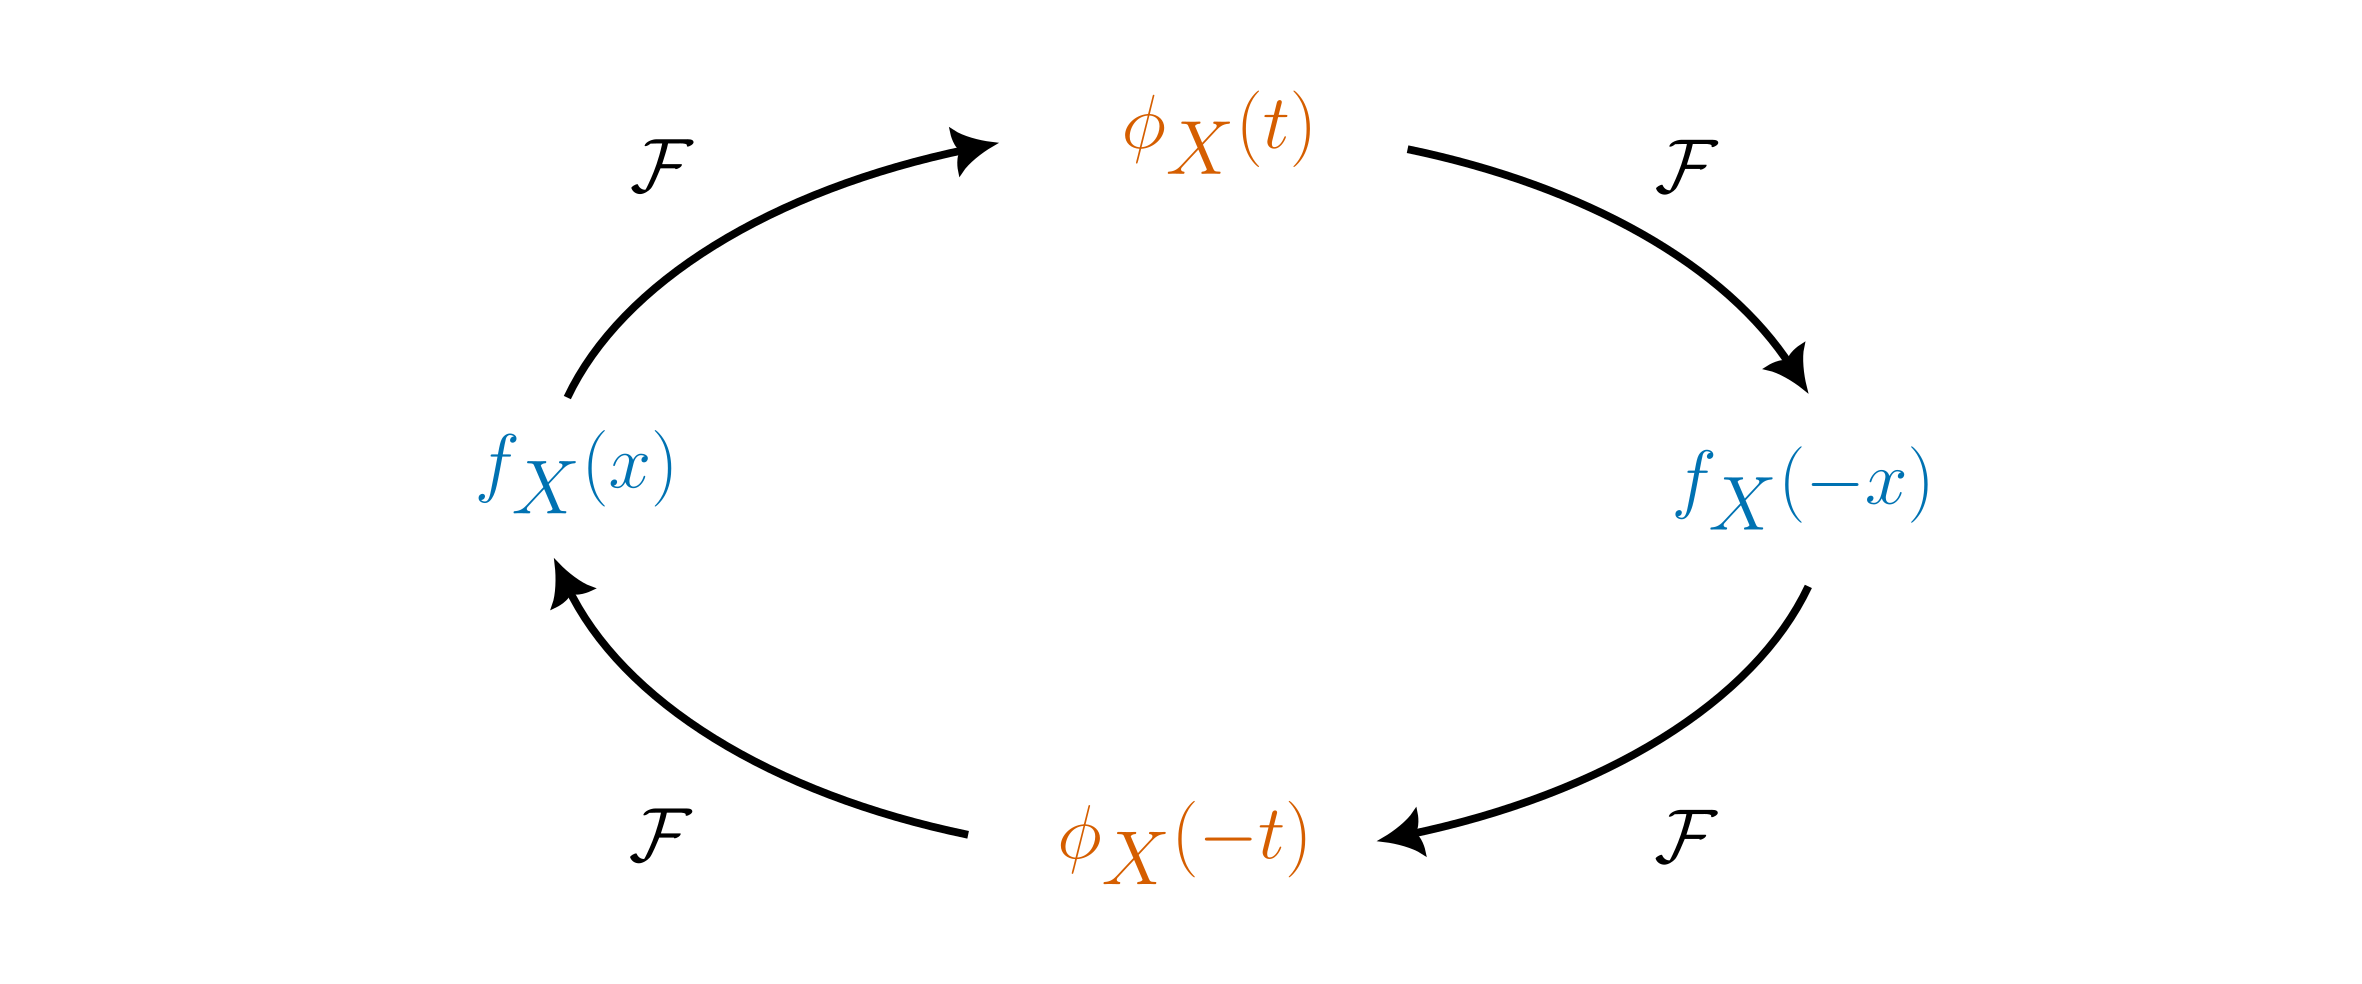
\includegraphics[width=\textwidth]{Figure 2.5.A}
\caption{The cyclical property of the Fourier transform $\mathcal F$}
\end{figure}
\noindent in which $\mathcal F (\mathcal F (\mathcal F(\mathcal F( \cdot ) ) ) )$ is \textbf{idempotent}\index{idempotent} and $\mathcal F(\mathcal F( \cdot ))$ is an \textbf{involution}\index{involution}. An idempotent function operating on an element returns the element itself, and an involutory function operating on an element returns the element's inverse.

In physics, if we $\psi_X(x)$ is the position wave function such that $|\psi_X(x)|^2 = f_X(x)$ is the probability density function of position, then:
$$\phi_A(a) = \frac{1}{\sqrt{2 \pi \hbar}} \int\limits_{-\infty}^\infty \psi_X(x) e^{\frac{- i a x}{\hbar}} dx$$
is the momentum wave function and $\hbar$ is the \textbf{reduced Planck constant}\index{reduced Planck constant}.

\section{Sufficient Statistics}
A \textbf{sufficient statistic}\index{sufficient statistic} $T(\boldsymbol X)$ for a random variable $X$ and probability distribution $f_X(x)$ and parameters $\boldsymbol \theta$ is said to contain all mutual information of $\boldsymbol \theta$ for a vector of random variable $\boldsymbol X = ( X_1, X_2,...,X_n) \sim f_X(x)$. This set $\boldsymbol X$ is said to be \textbf{independently and identically distributed}\index{independently and identically distributed} according to $f_X(x)$, and $T(\boldsymbol X)$ provides sufficient information to estimate $\boldsymbol \theta$. By utilizing the information gained from sufficient statistic $T$, the probability distribution for $\boldsymbol X$ paradoxically no longer depends on $\boldsymbol \theta$.\footnote{Given $T$, the parameter $\boldsymbol \theta$ likewise no longer depends on $\boldsymbol X$.}

Take the Bernoulli distribution:
$$f_X(x) = p^x (1-p)^{1-x}$$
for the vector of random observations $\boldsymbol X = \{X_1, X_2,...,X_n\}$ such that their \textbf{joint distribution}\index{joint distribution} is a function of multiple variables:
$$f_{X_1,...,X_n}(x_1,...,x_n)$$
However, we know that all elements of $\boldsymbol X$ follow the same distribution $f_X(x)$ such that:
$$f_{X_1,...,X_n}(x_1,...,x_n)$$
$$= f_{X_1}(x_1) \cdot f_{X_2}(x_2) \cdot ... \cdot f_{X_n}(x_n)$$
$$ = p^{x_1} (1-p)^{1-x_1} \cdot ... \cdot p^{x_n} (1-p)^{1-x_n} $$
We can summarize this joint distribution using product notation, or equivalently we may use summation notation in the exponent:
$$f_{X_1,...,X_n}(x_1,...,x_n) = \prod\limits_{i=1}^n f_{X_i}(x_i) $$
$$= \prod\limits_{i=1}^n p^{x_i} (1-p)^{1-x_i} = p^{\sum x_i} (1-p)^{\sum (1-x_i)}$$
The parameter $p$ only depends on the sufficient statistic $T(\boldsymbol X) = \sum x_i$, and the parameter has a most likely value of $p = \frac{1}{n} \sum x_i$, or the average.

This brings us to the \textbf{conditional probability}\index{conditional probability} interpretation of parameters. A probability distribution $f_X(x)$ given a parameter $ \theta$ is commonly written as $f_X(x | \theta)$ or $f_{X | \Theta}(x | \theta)$, reading as ``$f$ of $x$ given $\theta$''. A probability distribution $f_X(x|\theta)$ depends on an unknown parameter distribution $f_\Theta(\theta)$ which may be deterministic or stochastic. In fact, a fixed value for $\theta$ given by the \textbf{Dirac delta} distribution \index{Dirac delta} for some constant $\mu_\theta \in \Theta$:
$$f_\Theta(\theta) = \begin{cases} +\infty, \quad \theta = \mu_\theta \\ 0, \quad \textnormal{else}\end{cases}$$
is indistinguishable from a $\theta$ with low variance. We call $\Theta$ the \textbf{parameter space}\index{parameter space} of $\theta$ such that $\theta \in \Theta$.

The \textbf{likelihood function}\index{likelihood function} $\mathcal L (\theta | x)$ for a vector of realized observations $\boldsymbol x = (x_1,...,x_n)$ that are independently distributed, but not necessarily identically distributed with the same $\theta$, is given by:
$$\mathcal L(\theta | x) = \prod\limits_{i=1}^n f_i(x_i |\theta)$$
We determine the \textbf{log-likelihood function}\index{log-likelihood function} $\ell (\theta | x)$ to be given by $\ln(\mathcal L)$. It is often easier to work with the log-likelihood $\ell (\theta | x)$ for most of the frequently encountered distributions. The likelihood $\mathcal L$ may be interpreted as a probability distribution over $\theta$'s parameter space $\Theta$, but is not technically correct. Rather, it gives the relative frequency of observing the data set $\boldsymbol x$ under possible values of $\theta \in \Theta$.

There are two possible ways to obtain a nominal value for $\theta$: method of maximum likelihood and method of moments. The \textbf{method of maximum likelihood}\index{method of maximum likelihood} returns the \textbf{maximum likelihood estimate}\index{maximum likelihood estimate} (MLE) referred to as $\theta_{\textnormal{MLE}}$, and it is obtained by the formula:
$$\frac{\partial}{\partial \theta} \ell (\theta) = 0$$
then solving for $\theta$.\footnote{If there is no closed-form solution to isolate the parameter $\theta$, then numerical optimizers may be used to approximate.} Note that $\theta_{\textnormal{MLE}}$ is a function of the sufficient statistic $T(\boldsymbol X)$, and individual parameters of the set of parameters $\boldsymbol \theta$ may be codependent upon other parameters. 

The \textbf{method of moments}\index{method of moments} (MoM) estimate $\theta_{\textnormal{MoM}}$ is given by:
$$\mathrm{E}(g(X)) = h(\theta)$$
and solving for $\theta$. The simple and common choice is $g(X) = X$ such that:
$$\mathrm{E}(X) = \int\limits_{x \in X} x f_X(x)dx = h(\theta)$$
and solving for $\theta$ via $\theta = h^{-1}[\mathrm{E}(X) ]$.\footnote{If the inverse has no closed-form solution, we may also use a numerical optimizer.} The average or expectation $\mathrm{E}(X)$ is often substituted with the \textbf{sample average}\index{sample average} $\bar X$:
$$\bar X = \frac{1}{n} \sum\limits_{i=1}^n X_i$$

Infrequently, the MoM estimate is obtained via the formula:
$$\mathrm{Var}(X) = \int\limits_{x \in X} (x - \mathrm{E}(X))^2 f_X(x)dx = h(\theta)$$
and solving for $\theta$ as a function of $\mathrm{E}(X)$ and $\mathrm{Var}(X)$, replacing $\mathrm{E}(X)$ with the sample mean $\bar X$ and $\mathrm{Var}(X)$ with the sample second moment estimator:
$$\mathrm{Var}(X) = \frac{1}{n} \sum (X-\bar X)^2$$
The $k$-th method of moment estimator is given by:
$$\theta^{(k)}_{\textnormal{MoM}} = \frac{1}{n} \sum\limits{i=1}^n X^k$$
Note that the method of moments estimator $\theta_{\textnormal{MoM}}$ is not guaranteed to be an element of the parameter space $\Theta$. If computing the maximum likelihood estimator $\theta_{\textnormal{MLE}}$ is difficult and requires successive approximations, then the method of moments estimator is a reasonable starting point for parameter optimization algorithms.

\section{Exponential Families}
\textbf{Exponential families}\index{exponential family} refer to a class of probability distribution in which each probability density function $f_X(x|\theta)$ may be written as the product:
$$f_X(x|\theta) = h(x) \cdot g(\theta) \cdot e^{\eta (\theta) \cdot T (x)}$$
in which $\eta$ is the \textbf{natural parameter}\index{natural parameter}, $T (x)$ is the \textbf{sufficient statistic}\index{sufficient statistic} of parameter set $\theta$ or natural parameter set $\eta$, and $g(\theta)$ is the normalization constant such that:
$$\int\limits_{x \in X} h(x) \cdot e^{\eta \cdot \boldsymbol T} = [g(\theta)] ^{-1}$$
In simpler terms, $g$ is the constant that normalizes the distribution to sum to $1$. We alternatively may prefer the notation $g(\theta) = e^{A(\theta)}$ and $h(x) = e^{B(x)}$. The normalizing factor $g(\theta)$ is called the \textbf{partition function}\index{partition function}, although we usually work with $A(\theta)$ and refer to it as the \textbf{log-partition function}\index{log-partition function}. We may generalize our notation to work for vector parameters and vector variables using bold symbols:
$$f_{\boldsymbol X}(\boldsymbol x|\boldsymbol \theta) = h(\boldsymbol x) \cdot g(\boldsymbol \theta) \cdot e^{\boldsymbol{\eta (\theta)} \cdot \boldsymbol{T (x)}}$$
In this case, we are referring to $\boldsymbol x$ as a multivariate vector of the multivariate random variable $\boldsymbol X$ instead a vector of independent observations when we write $\boldsymbol x$.

%\newpage

The key properties of exponential families for which $h(\boldsymbol x) > 0$, $\boldsymbol{\eta(\theta)}$, $\boldsymbol{T(x)}$, $A(\boldsymbol \theta)$ are known functions are as follows:
\begin{enumerate}
\item Sufficient statistics $\boldsymbol T(x)$ are countably finite and exist for any $n \in \mathbb N$ for independent and identically distributed $\boldsymbol X = (X_1,...,X_n)$.
\item The exponential family $f_{\boldsymbol X} (\boldsymbol x | \boldsymbol \theta)$ has a probability density function $f_{\boldsymbol \Theta}(\boldsymbol \theta$) on its parameter vector $\boldsymbol \theta$ that is also an exponential family, referred to as a \textbf{conjugate prior}\index{conjugate prior}\index{prior distribution}. The likelihood function $\mathcal L(\boldsymbol \theta)$ in this case is a valid probability density function on $\boldsymbol \theta$ for future identical arrivals of $\boldsymbol x$.
\item The \textbf{natural parameter space}\index{natural parameter space} $\boldsymbol H$ for which $\boldsymbol \eta \in \boldsymbol H$ is always convex.
\item The natural exponential family has the property for $p_{\boldsymbol H}(\boldsymbol \eta), \boldsymbol \eta \in \boldsymbol H$:
$$\mathrm{E}_{\boldsymbol H}(\boldsymbol {T(X)}) = \nabla A(\boldsymbol \eta)$$
$$\quad \mathrm{Cov}_{\boldsymbol H}(\boldsymbol {T(X)}) = \nabla^2 A(\boldsymbol \eta)$$
\end{enumerate}
Natural exponential families are therefore fully characterized by the first and second derivative of the log-partition function with respect to the natural parameter vector $\boldsymbol \eta$. 

For the individual portions of the sufficient statistics, the first and second partial derivatives with respect to the corresponding natural parameter gives the key information about that sufficient statistic:
$$\mathrm{E}_{\boldsymbol H}[T_i(\boldsymbol X)] = -\frac{\partial}{\partial \eta_i} \ln (g(\boldsymbol \eta)) = \frac{\partial}{\partial \eta_i} A(\boldsymbol \eta)$$
$$\mathrm{Cov}_{\boldsymbol H}[T_i(\boldsymbol X), T_j(\boldsymbol X)] = -\frac{\partial^2}{\partial \eta_i \partial \eta_j} \ln g((\boldsymbol \eta)) = \frac{\partial^2}{\partial \eta_i \partial \eta_j} A(\boldsymbol \eta)$$
The expectation vector and covariance matrix are the first and second \textbf{cumulants}\index{cumulant} respectively of the \textbf{cumulant-generating function}\index{cumulant-generating function} $A(\eta)$. These two cumulants fully characterize the information of the natural exponential family. If for example a normal distribution has a natural parameter vector $(\eta_1, \eta_2)$ with sufficient statistics vector $(x, x^2)$, then $\frac{\partial^2}{\partial \eta_1 \partial \eta_2} A(\eta) = \mathrm{Cov}(X, X^2)$.

This gives us a beautiful formulation of the connection between natural parameters and sufficient statistics by relating the mutual information of derivatives and anti-derivatives. Consider that $[g(\eta)]^{-1} = \mathrm{E}[g(\eta)^{-1}]$ such that $A(\eta) = -ln(\mathrm{E}[g(\eta)])$. Then:
$$\mathrm{E}_{\boldsymbol H}[\boldsymbol{T(X)}] = -\nabla_{\boldsymbol \eta} \ ln(E_{\boldsymbol X}[g(\boldsymbol \eta)])$$
$$\mathrm{Cov}_{\boldsymbol H}[\boldsymbol{T(X)}] = -\nabla_{\boldsymbol \eta}^2 \ ln(E_{\boldsymbol X}[g(\boldsymbol \eta)]) = \mathcal I (\boldsymbol \eta)$$
The first cumulant is sometimes referred to as the score or informant and the second cumulant $\mathcal I (\boldsymbol \eta)$ is the variance of the score, but it is more commonly called the Fisher information matrix.

The \textbf{Fisher information}\index{Fisher information} matrix $\mathcal I(\boldsymbol \eta)$ is derived as the form:
$$\mathcal I (\boldsymbol \theta) = -\mathrm{E}(\nabla^2_{\boldsymbol \theta} \ln [f(\boldsymbol x | \boldsymbol \theta)])$$
under special regularity conditions. If those regularity conditions are not met, the Fisher information may be derived more generally as:
$$\mathcal I (\boldsymbol \theta) = \mathrm{E}([\nabla_{\boldsymbol \theta} \ln [f(\boldsymbol x | \boldsymbol \theta)]^T [\nabla_{\boldsymbol \theta} \ln [f(\boldsymbol x | \boldsymbol \theta)])$$
The Fisher information is a positive semi-definite matrix, meaning $\mathcal I(\boldsymbol \theta) \geq 0$ for all entries. Recall that the natural parameter space $\boldsymbol H$ is always convex, therefore $\mathcal I(\boldsymbol \eta)$ for a single observation of the random variable $\boldsymbol X$ has a guaranteed global maximum. This is important as Fisher information $\mathcal I(\boldsymbol \theta)$ is additive for multiple observations of $(\boldsymbol X_1,...,\boldsymbol X_n)$. These multiple observations will cluster around the maximum likelihood estimate, and the maximum likelihood estimate will become steeper as the number of observations $n$ increases. However, the maximum likelihood estimates have a key limitation.

Note that $\mathcal I(\boldsymbol \theta) \geq 0$ is not true for mixtures of normal distributions. A probability distribution that is composed of two different normal distributions with $\sigma^2 = \sigma_1^2 = \sigma_2^2$ and $\mu_2 = \mu_1 + 2\sigma$ will have two peaks in the log-likelihood function $\ell (\boldsymbol \theta)$. In these fixed values cases, the optima of $\ell (\boldsymbol \theta)$ for exponential family converges as $n \rightarrow \infty$. If $\mathcal I(\boldsymbol \theta) \geq 0$ for all $\boldsymbol \theta$ in $\boldsymbol H$, then the statistical model is regular. Else, the model is irregular or singular. Other statistical models that are irregular are other mixture distributions, neural networks, and hidden Markov models.

If each parameter of the parameter vector $\boldsymbol \theta$ is instead a random variable drawn from the parameter space $\boldsymbol \Theta$ with probability distribution $f_{\boldsymbol \Theta}(\boldsymbol \theta)$, then our observed likelihood function $\ell(\boldsymbol \theta)$ will instead converge upon $\ln(f_{\boldsymbol \Theta}(\boldsymbol \theta))$. If the probability density function $f_{\boldsymbol X}(\boldsymbol x | \boldsymbol \theta)$ is of the form of an exponential family, then so is the conjugate prior distribution $f_{\boldsymbol \Theta}(\boldsymbol \theta)$. While $f_{\boldsymbol X}(\boldsymbol x | \boldsymbol \theta)$ is a theoretical construct of the distribution of $\boldsymbol x \in \boldsymbol X$ for a fixed parameter vector $\boldsymbol \theta$, the likelihood function $\mathcal L(\boldsymbol \theta | \boldsymbol x)$ instead represents the distribution of $\boldsymbol \theta \in \boldsymbol \Theta$ for a fixed set of observations $(\boldsymbol x_1,...,\boldsymbol x_n)$. 

We may therefore ask for the integral to obtain the distribution for $\boldsymbol X$ that no longer depends on $\boldsymbol \theta$:
$$f_{\boldsymbol X}(\boldsymbol x) =\int\limits_{\boldsymbol \theta \in \boldsymbol \Theta} \ell(\boldsymbol \theta | \boldsymbol x) f_{\boldsymbol \Theta}(\boldsymbol \theta) d \boldsymbol \theta$$
in which $f_{\boldsymbol \Theta}(\theta) = 1$ represents our ignorance of the distribution of $\boldsymbol \theta$. This unconditional distribution $f_{\boldsymbol X}(\boldsymbol x)$ is the distribution in which $f(\boldsymbol x | \boldsymbol \theta) = \mathcal L( \boldsymbol \theta | \boldsymbol x)$ for fixed values for each data point $\boldsymbol x$.

If we wish to determine a posterior distribution for $\boldsymbol \theta$ knowing $\boldsymbol x$, we calculate the following probability distribution:
$$f(\boldsymbol \theta | \boldsymbol x) = \frac{f(\boldsymbol x | \boldsymbol \theta) f(\boldsymbol \theta)}{f(\boldsymbol x)} $$
According to the definition of sufficient statistics, our distribution fors $\boldsymbol \theta$ and $\boldsymbol x$ should be independent of each other if we are given the sufficient statistic.
If you recall the properties of exponential families, we can show that the expected value of our natural parameters should be derivable from its own version of the cumulant-generating function:
$$\mathrm{E}_{\boldsymbol X}[\eta_i(\boldsymbol \theta)] = -\frac{\partial}{\partial T_i} \ln(h(\boldsymbol x))$$
$$\mathrm{Cov}_{\boldsymbol X}[\eta_i(\boldsymbol \theta), \eta_j(\boldsymbol \theta)] = -\frac{\partial^2}{\partial T_i \partial T_j} \ln(h(\boldsymbol x)) $$
We might call $B(\boldsymbol x) = -\ln(h(\boldsymbol x))$ to be the corresponding cumulant-generating function. It is this symmetry that is fundamental to exponential family distributions. This is not a guarantee that the conjugate prior is necessarily a known or common exponential family member.

\section{Conditional Probability}
A \textbf{conditional probability}\index{conditional probability} density function $f_X(x|A)$ is when a probability distribution $f_X(x)$ is said to be given a condition $A$ . This condition $A$ may be any set condition on values of the random variable such as $A= (x \in S)$ or $A= (x < 0)$. We define $f_X(x) = f_X(x|x \in X)$ being no conditions or default conditions applied to the distribution.

The most common use for conditional distribution notation is for describing parameters $\theta$ of a distribution via $f(x|\theta)$, sums of random variables, or combinatoric events such as card game hands (e.g. a straight as a poker hand). Ironically, conditional probability for sums is more complicated than either parameters or card games.

A conditional probability function $f_X(x|A)$ is said to be independent of condition $A$ if and only if:
$$f_X(x|A) = f_X(x)$$
Likewise, two probability functions $f_X(x)$ and $f_Y(y)$ are said to be \textbf{statistically independent}\index{statistically independent} if and only if:
$$f_{X,Y}(x,y) = f_X(x) \cdot f_Y(y)$$
since the regular case is for separating a joint distribution $X,Y$ is given by:
$$f_{X,Y}(x,y) = f_{X|Y}(x|y) \cdot f_Y(y) = f_X(x) \cdot f_{Y|X}(y|x) $$
For example, two dice rolls upon $(X,Y)$ are independently rolled, but the height of a mountain given coordinates $(X, Y)$ is not independent per coordinate.

The rules of conditional probability give us three different looking but equivalent statements that define \textbf{statistical independence}\index{statistical independence}:
\begin{enumerate}
\item $f(x, y) = f(x) f(y)$
\item $f(x|y) = f(x)$
\item $f(y|x = f(y)$
\end{enumerate}
This brings us to three equivalent statements about sufficient statistic $T$ for a data vector $\boldsymbol x$ and parameter value $\boldsymbol \theta$:
\begin{enumerate}
\item $f(\boldsymbol \theta, \boldsymbol x | T) = f(\boldsymbol \theta | T) f(\boldsymbol x | T)$
\item $f(\boldsymbol \theta | \boldsymbol x, T) = f(\boldsymbol \theta | T)$
\item $f(\boldsymbol x| \boldsymbol \theta, T) = f(\boldsymbol x | T)$
\end{enumerate}
This third statement is what we mean that our original data vector $\boldsymbol x$ paradoxically no longer depends on $\boldsymbol \theta$ during \textit{\S 2.6 Sufficient Statistics}. The sufficient statistic $T$ provides all the information necessary for the distribution of $\boldsymbol x$.

Using the above relation, we may state \textbf{Bayes' theorem}\index{Bayes' theorem}:
$$f(x|y) = \frac{f(y|x) f(x)}{f(y)} = \frac{f(x, y)}{f(y)}$$
in which $X, Y$ are random variables under the \textbf{joint probability}\index{joint probability} density function $f(x,y)$.

\section{Law of Large Numbers}
The \textbf{law of large numbers}\index{law of large numbers} is a mathematical law about how the average of a set of random variables. There are two version of the law: the weak law and the strong law.

The \textit{weak law of large numbers}\index{weak law of large numbers} states that for a set of independently and identically distributed random variables $X_1,...,X_n \sim f_X(x)$ that the sample average $\bar X = (1/n)\sum X_i$ obeys the following properties:
$$ \underset{n \rightarrow \infty}{\lim} P (|\bar X_n - \mu| < \varepsilon) = 1$$
if $\mathrm{Var}(X) = \sigma^2 < \infty$ and any $\varepsilon > 0$. What this means to say is that the \textit{limit of the probability} that a sample average $\bar X$ is within some margin $(-\varepsilon, +\varepsilon)$ converges to probability $1$ as you increase the number of samples of $X \sim f_X(x)$.

The \textit{strong law of large numbers}\index{strong law of large numbers} states that for a set of independently and identically distributed random variables $X_1,...,X_n \sim f_X(x)$ that the sample average $\bar X = (1/n)\sum X_i$ obeys the following properties:
$$ P (\underset{n \rightarrow \infty}{\lim}|\bar X_n - \mu| < \varepsilon) = 1$$
if $\mathrm{Var}(X) = \sigma^2 < \infty$ and any $\varepsilon > 0$. What this means to say is that the \textit{probability of the limit} that a sample average $\bar X$ is within some margin $(-\varepsilon, +\varepsilon)$ is necessarily probability $1$ as you increase the number of samples of $X \sim f_X(x)$.

The limit of the probability versus the probability of the limit has subtly different implications. The strong law implies the weak law, but not the other way around. This is because the strong law is stricter on how it defines its relationship to variance. The strong law basically says that \textit{there exists some} $n$ for which $\mathrm{Var}(\bar X) < \varepsilon^2$. Therefore, the probability of the limit is $1$. The weak law basically says that the probability $\mathrm{Var}(\bar X) < \varepsilon^2$ is $1-1/n$. Therefore, the limit of the probability is $1$.

\chapter{Random Walks}
\section{Motivations for Learning Random Walks}
\textbf{Random walks}\index{random walk} are the simplest random system: a point traveling through space according to a coin flip, a die roll, or more generally the random selection of the face of an $n$-cube:
\begin{figure}[H]
\centering
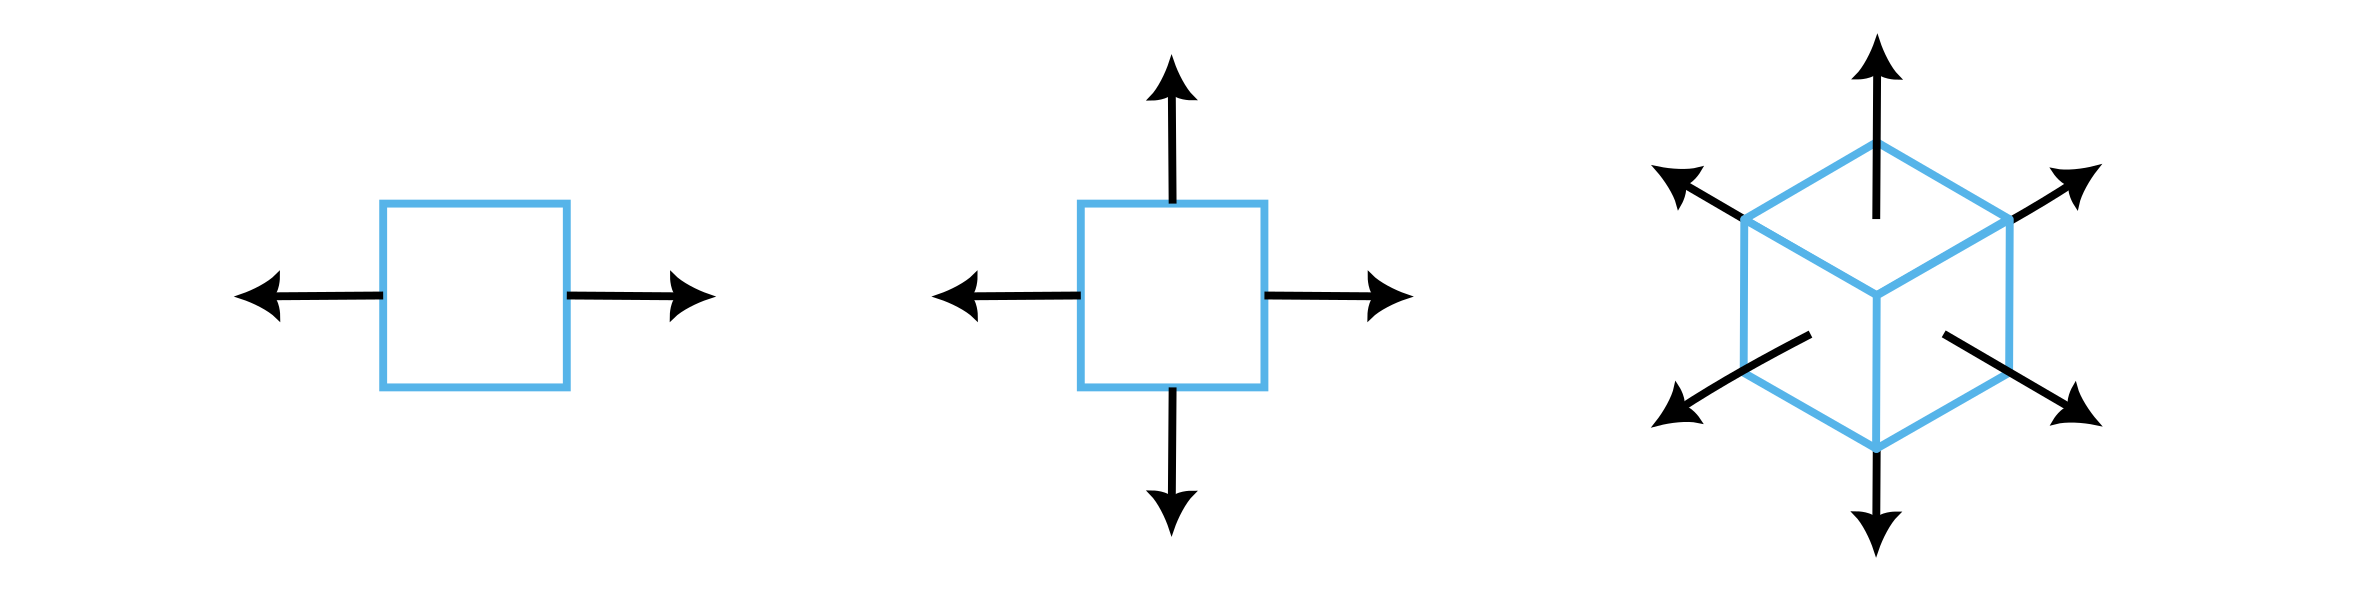
\includegraphics[width=\textwidth]{Figure 3.1.A}
\caption{Random walkers in 1D, 2D, and 3D}
\end{figure}
\noindent It seems poetic then that the simplest stochastic system, combined with the simplest non-trivial set $\mathbb B_\pm = \{ -1, 1\}$ results in an emergent complexity that is fully capable of simulating any other random computer. Perhaps even the universe.

Random walks are often considered stepping stones to more complex stochastic processes such as Wiener processes (more commonly known as Brownian motion) and Poisson processes. In our case, random walks are the goal and focal point of study. It is precisely its childish simplicity and mathematical purity that has caused us to discount its potential physical universality.

Random walks have various properties to consider before we directly describe Boolean random walks in this chapter. While we touch upon the solution of Boolean random walks quite early in this textbook, its significance requires a much deeper explanation over different mathematics topics. In physics, we may say that for the ``particles in a box'' model that:
\begin{figure}[H]
\centering
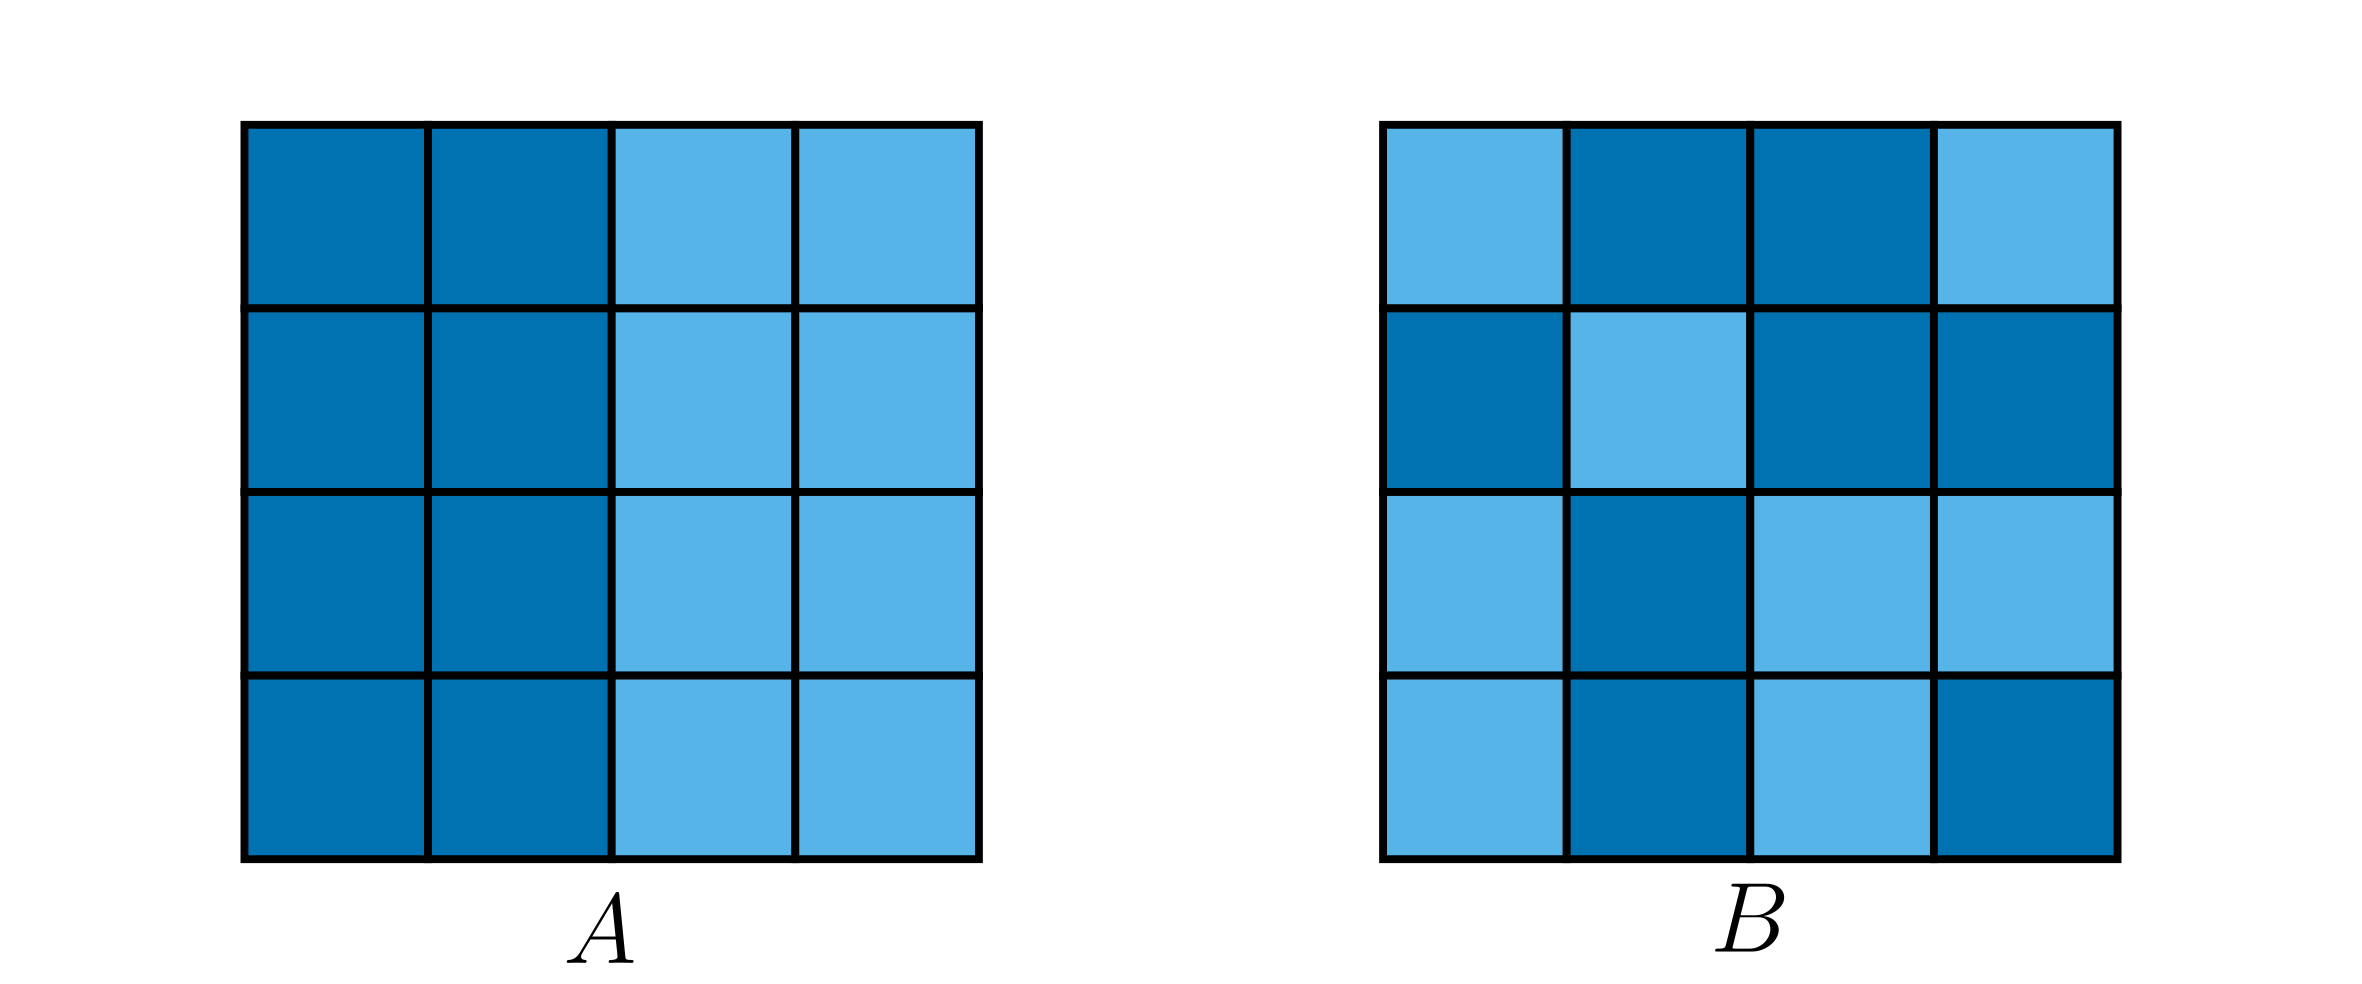
\includegraphics[width=\textwidth]{Figure 3.1.B}
\caption{Two states in which $A$ is more orderly than $B$}
\end{figure}
\noindent
State $A$ is lower entropy than State $B$, or rather we say that $A$ is more orderly than $B$. We may know intuitively what that means, but we lack a good definition that matches our intuition. We need a mathematical object with which to study orderliness of physical space. Boolean random walks can help us define entropy of physical spaces.

\section{Simple Random Walks}
The \textbf{simple random walk}\index{simple random walk} describes the movement of a point on the integer lattice $\mathbb Z^d$ in which the dimension of movement is randomly sampled from $\{ 1,...,d\}$ and the magnitude of movement is randomly sampled from $\mathbb B_\pm = \{ -1, 1\}$. The rectangular lattice of dimension $d=1$ is the simplest, describing a point or block randomly moving left or right by distance $1$ per time step of length $1$.
\begin{figure}[H]
\centering
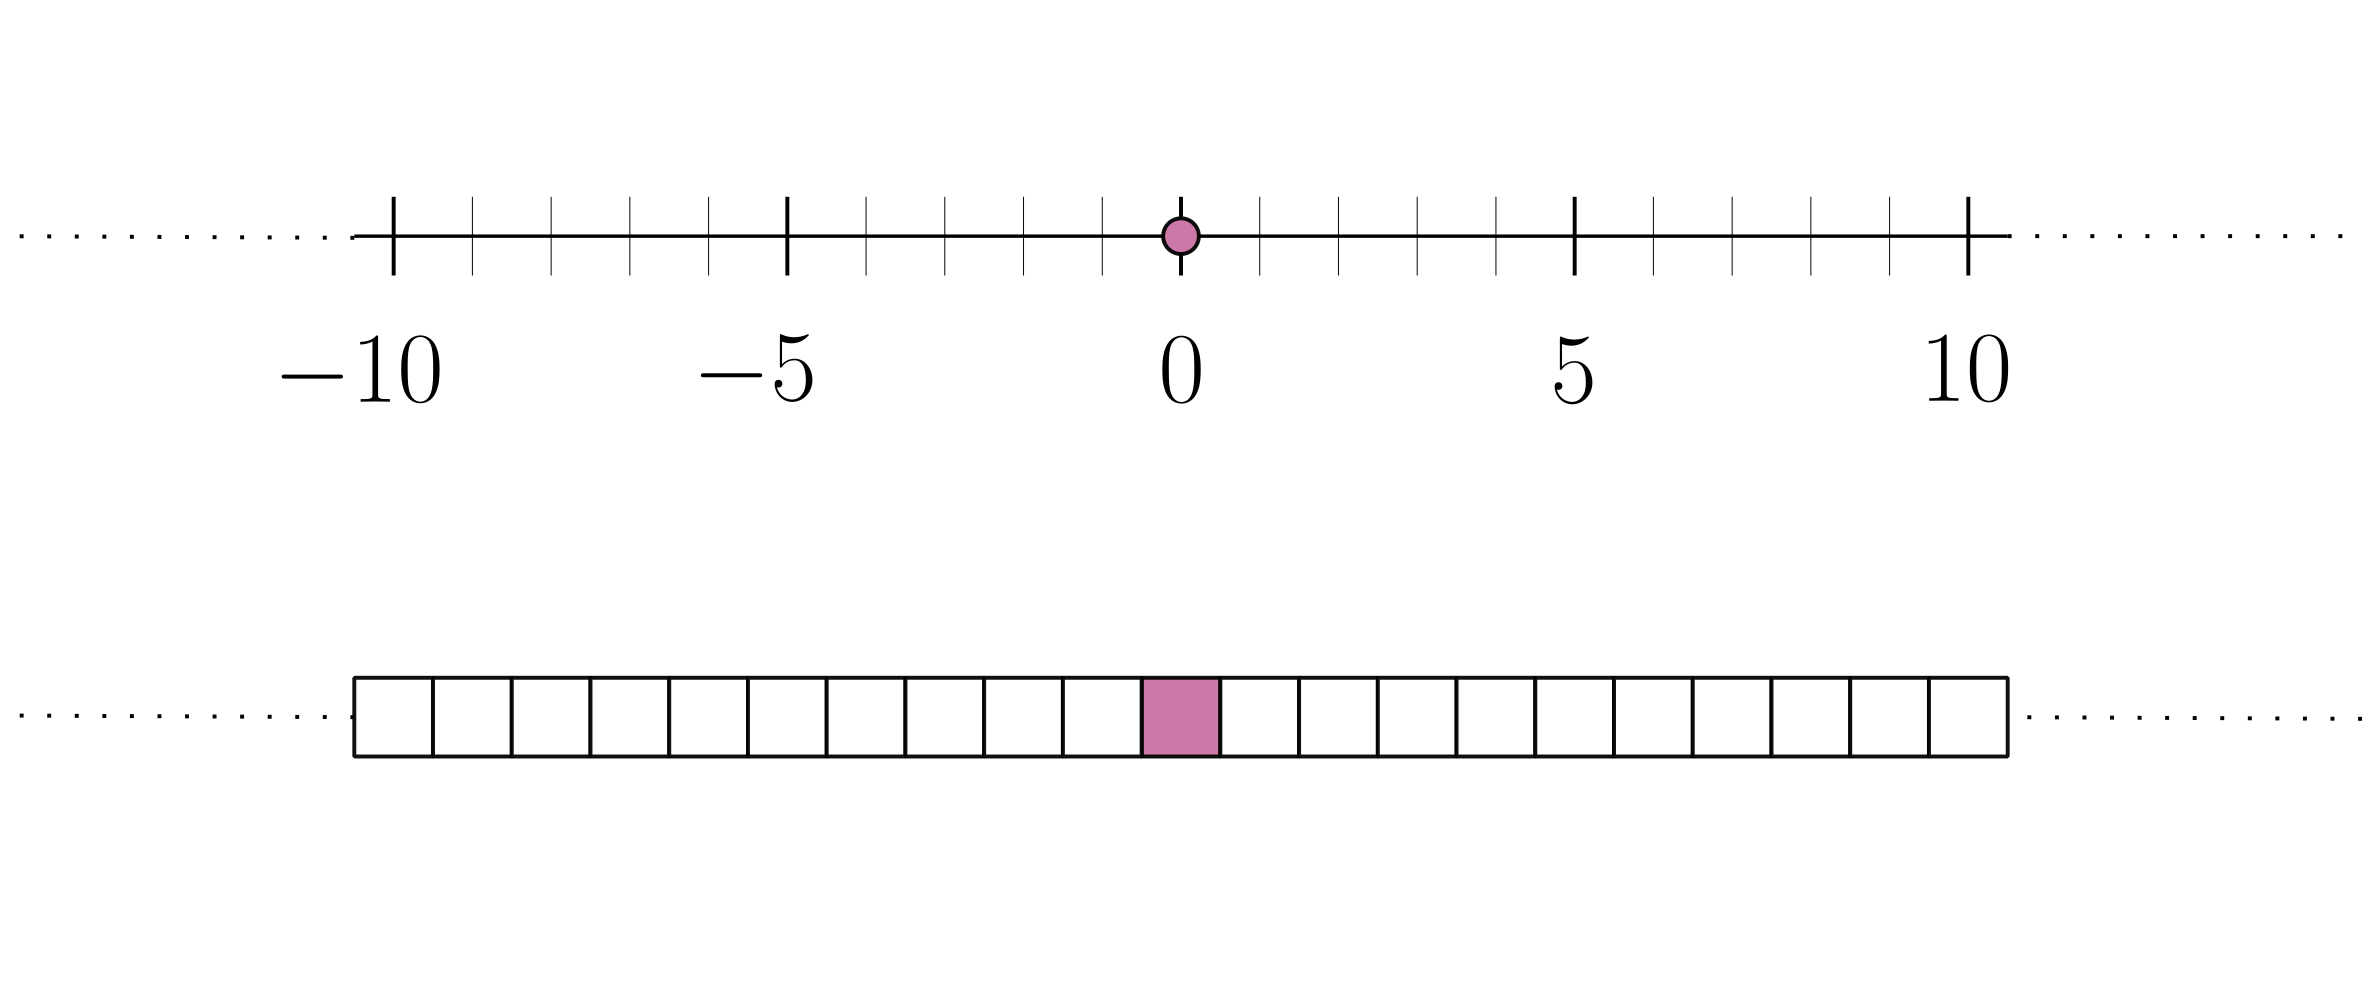
\includegraphics[width=\textwidth]{Figure 3.2.A}
\caption{Two representations of a random walker}
\end{figure}
\noindent
Simple random walks begin at the origin and have equal probability in moving in each direction across all $d$-dimensions. We describe this random walk as a random variable $X_t$ or $X(t)$ due to its value being a function of time variable $t$. It is called a random process or \textbf{stochastic process}\index{stochastic process} because the function value changes randomly at each step forward in time.

Each space or cell in $\mathbb Z^d$ is considered even or odd just like a checkerboard. Since we begin at the origin $X_0 = (0,...,0)$ at time $t=0$, the value of $X_t$ is always even for even time $t$ or odd for odd time $t$. A random walk is thus called a $2$-periodic process because it may never return to its current state in less than $2$ time cycles in the process.\footnote{A system that may stay the same after one time step for every state is called aperiodic.} Furthermore, consider the random variable $X_1$: its average position is at the origin, $\mathrm{E}(X_t) = 0$, despite not being able to inhabit the origin at odd time steps $t$. 

As discussed during \textit{\S 2.9 Law of Large Numbers}, the distribution of mean or sum of multiple random variables converges to the normal distribution. That same principle follows for random walks, and it behaves similarly to the binomial distribution. While the random walk process $X_t$ has a probability distribution that is approximately smooth as $t \rightarrow \infty$, its realized value $x_t \in X_t$ must have a parity that matches the parity of time $t$, $(x_t \mod 2) = (t \mod 2)$.

One of the key properties of a simple random walk is that $\mathrm{Var}(X_t)=t$. In order to show this is always true in any dimension, we begin with a single step in a random walk. For $d$-dimensions, the random variable $Z$ for the random walk of a $d$-dimensional cube is always $1$:
$$\mathrm{Var}(Z) = \sum\limits_{i=1}^d \frac{1}{d} [\frac{1}{2}(1)^2 + \frac{1}{2} (-1)^2] = 1$$
Using the sum of independent random variables property that:
$$\mathrm{Var}(Z_1 +...+ Z_t) = \mathrm{Var}(Z_1) + ... + \mathrm{Var}(Z_t)$$
We may therefore compute that:
$$\mathrm{Var}(X_t) = \sum\limits_{i=1}^t \mathrm{Var}(Z_i) = \sum\limits_{i=1}^t 1 = t$$
Together, the properties $\mathrm{E}(X_t) = 0$ and $\mathrm{Var}(X_t)=t$ describe the radial or circular dispersion of a particle on a grid.

\section{Bounded Random Walks}
A \textbf{bounded random walk}\index{bounded random walk} is a random walk whose domain is restricted to a finite of states called the state space $\mathcal X$. The power set $2^{\mathcal X}$ denotes all possible connections of the state space. Observe the following bounded random walk system $X$ represented by the graph below:
\begin{figure}[H]
\centering
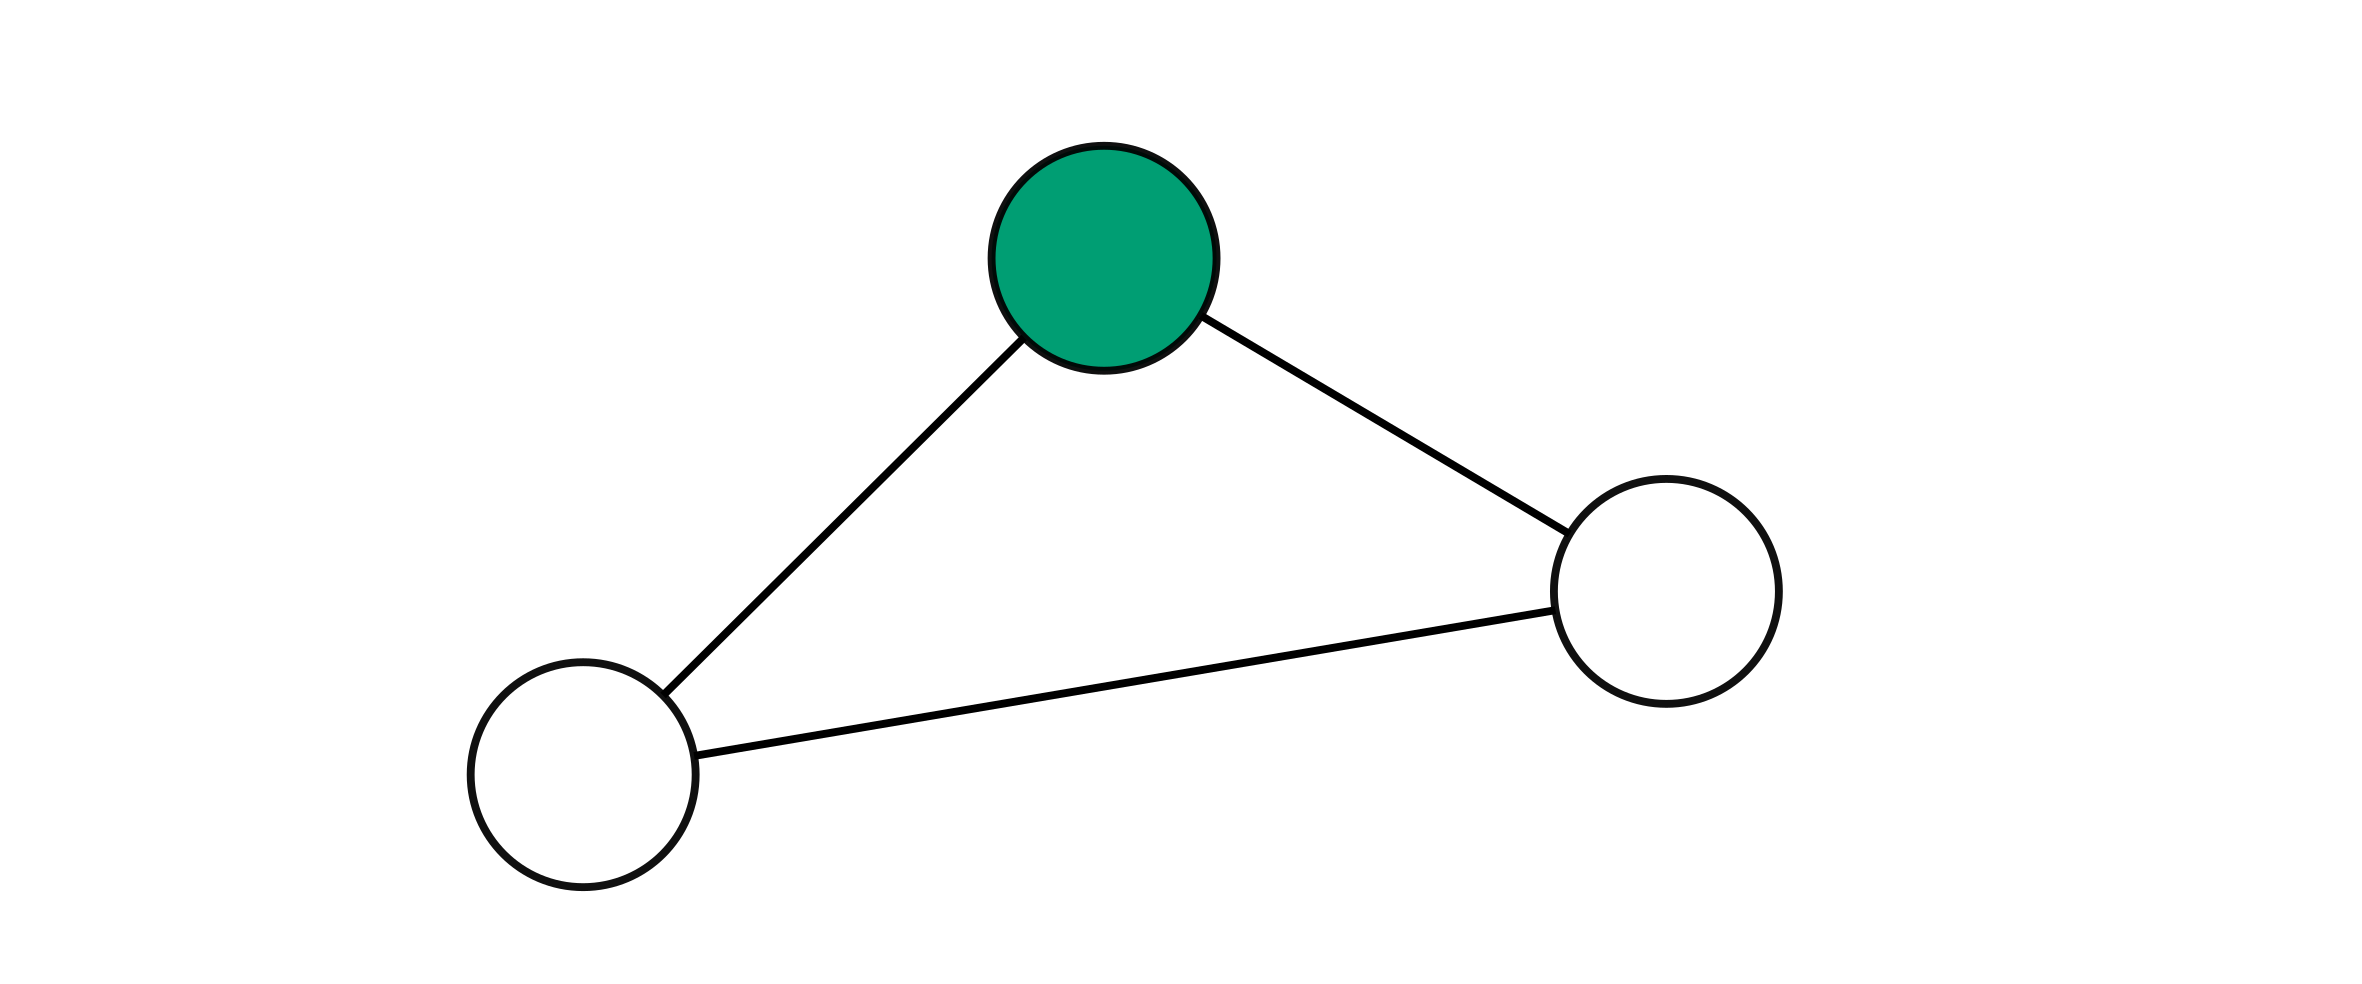
\includegraphics[width=\textwidth]{Figure 3.3.A}
\caption{A bounded random walker on the complete graph $K_3$}
\end{figure}
\noindent in which the particle may only move to empty adjacent cells with equal probability. This toy example with a helps us gain an intuition of how deal with random walks that are only on a subset of a rectangular lattice:
\begin{figure}[H]
\centering
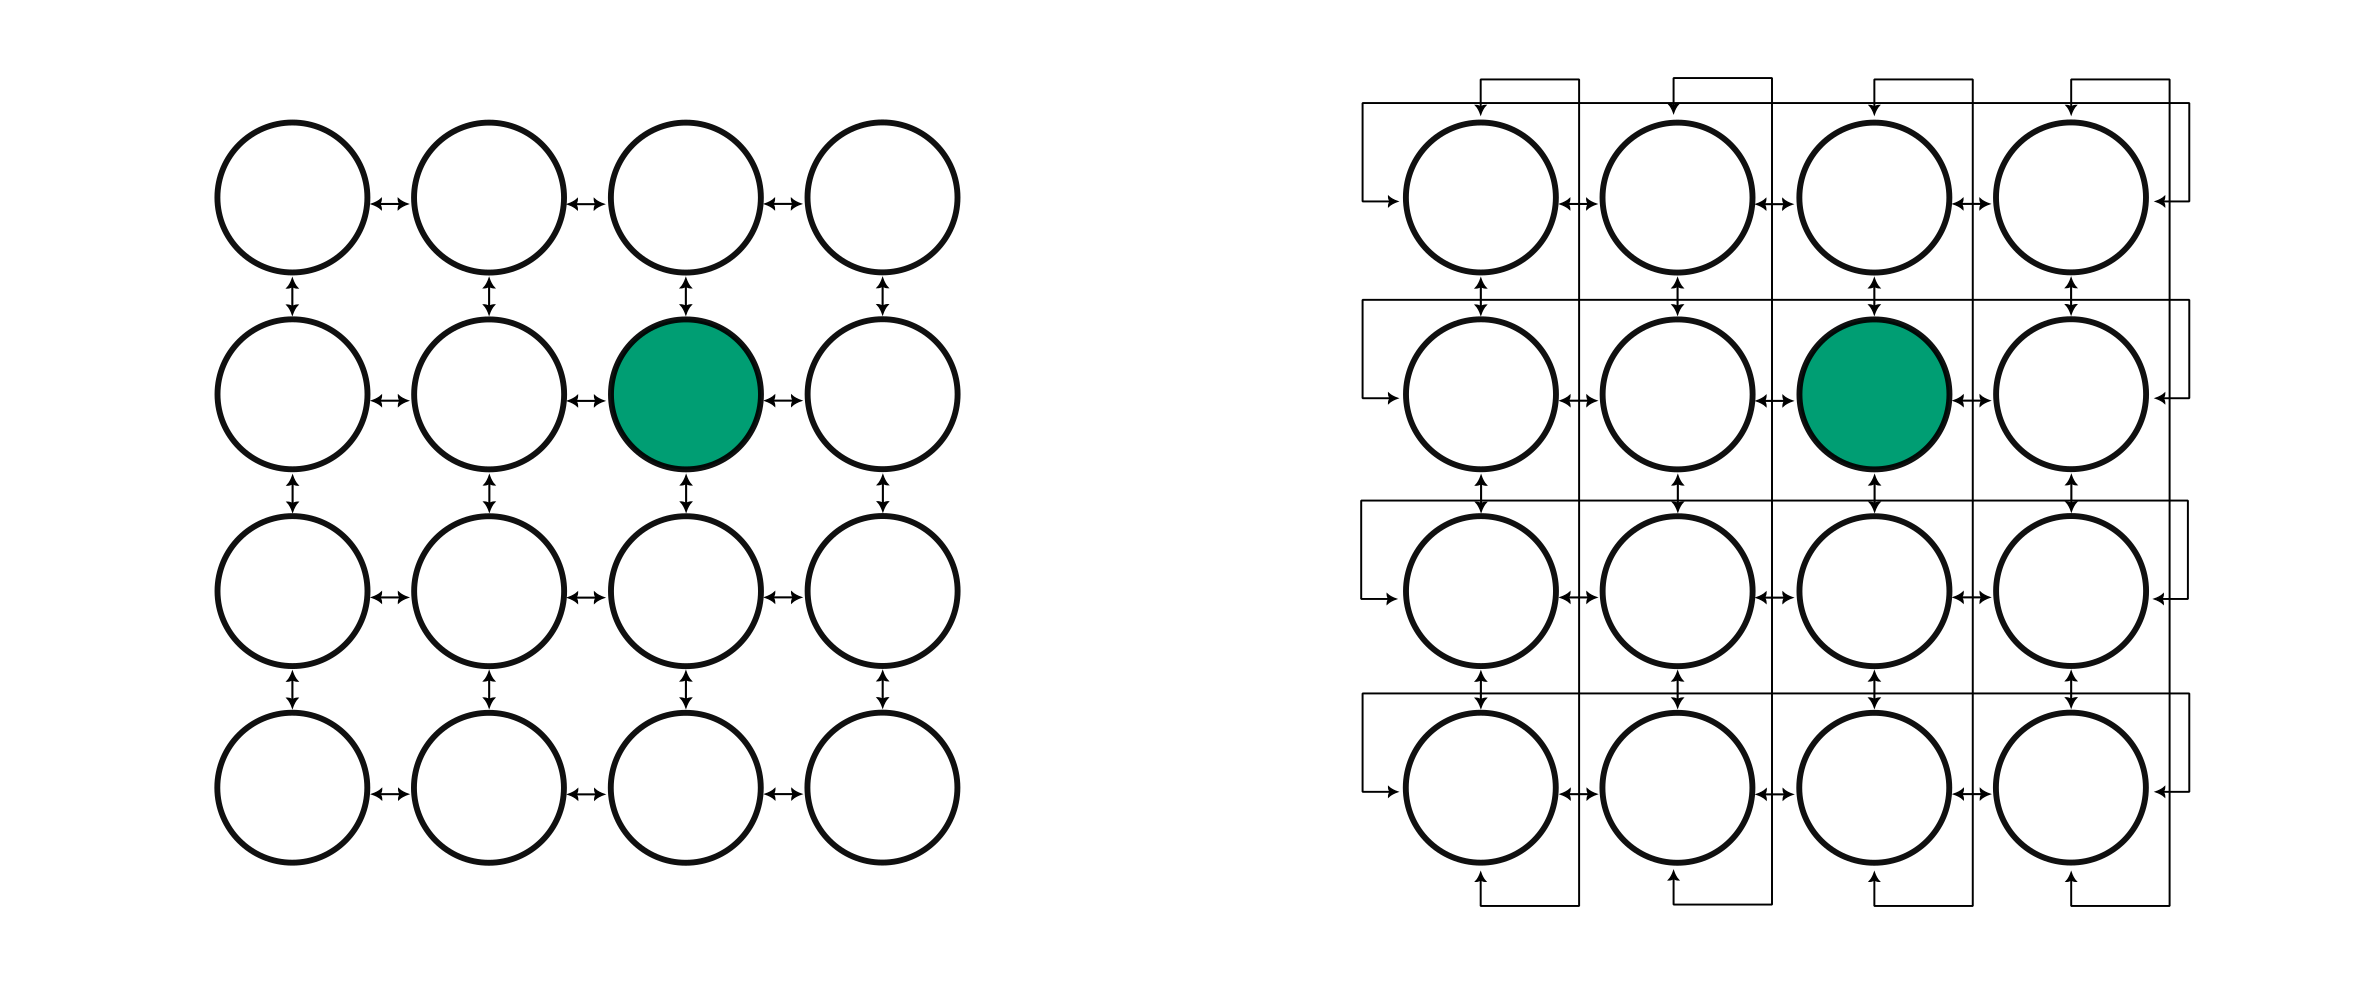
\includegraphics[width=\textwidth]{Figure 3.3.B}
\caption{Reflecting vs looping walls of a bounded random walk}
\end{figure}
We usually omit the edges of connection and represent the vertices of the graph as cells on graph paper, and we instead specify if the sytem $X$ is reflecting or looping. Vertices are sometimes called nodes or cells. The rectangular cell notation is very compact and convenient.
\begin{figure}[H]
\centering
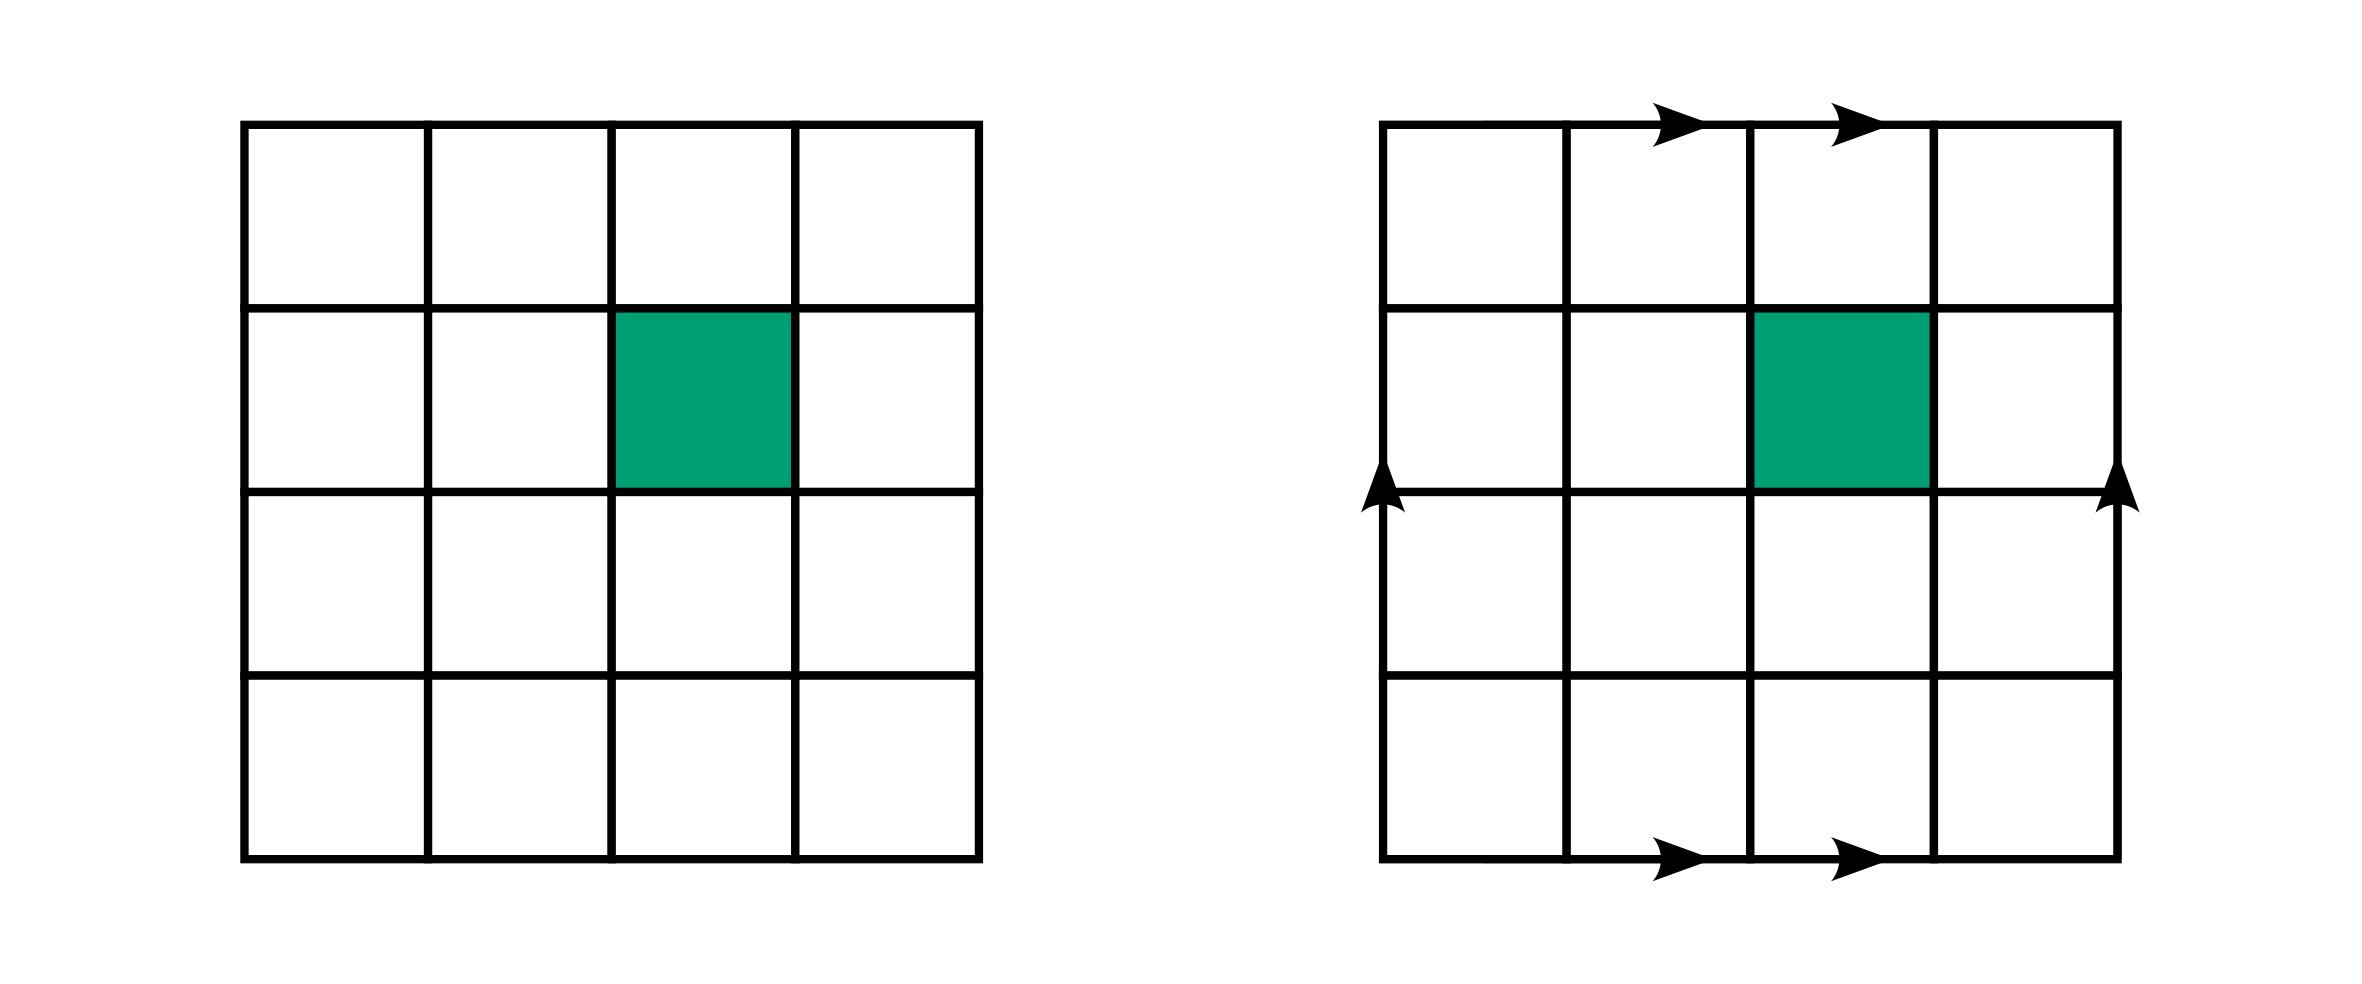
\includegraphics[width=\textwidth]{Figure 3.3.C}
\caption{Compressed notation of a bounded random walk}
\end{figure}

Boundaries are necessary for the simulation of any random walk process with more than one type or class of particle. A simple random walk needs no boundaries to simulate, and it is computationally indistinguishable from a single particle in an infinite antiparticle sea. What can a finite Boolean random walk simulation have in order to roughly simulate contact with an infinite mixture of particles and antiparticles?

Let $W_t$ be the \textbf{boundary noise function}\index{boundary noise function} operating on the system $X_t$. It randomly populates cells at the boundary of $X_t$, defined as $\partial X_t$, according to some distribution of possible cell values (e.g. $\mathbb B = \{-1, +1\}$) over time:
\begin{figure}[H]
\centering
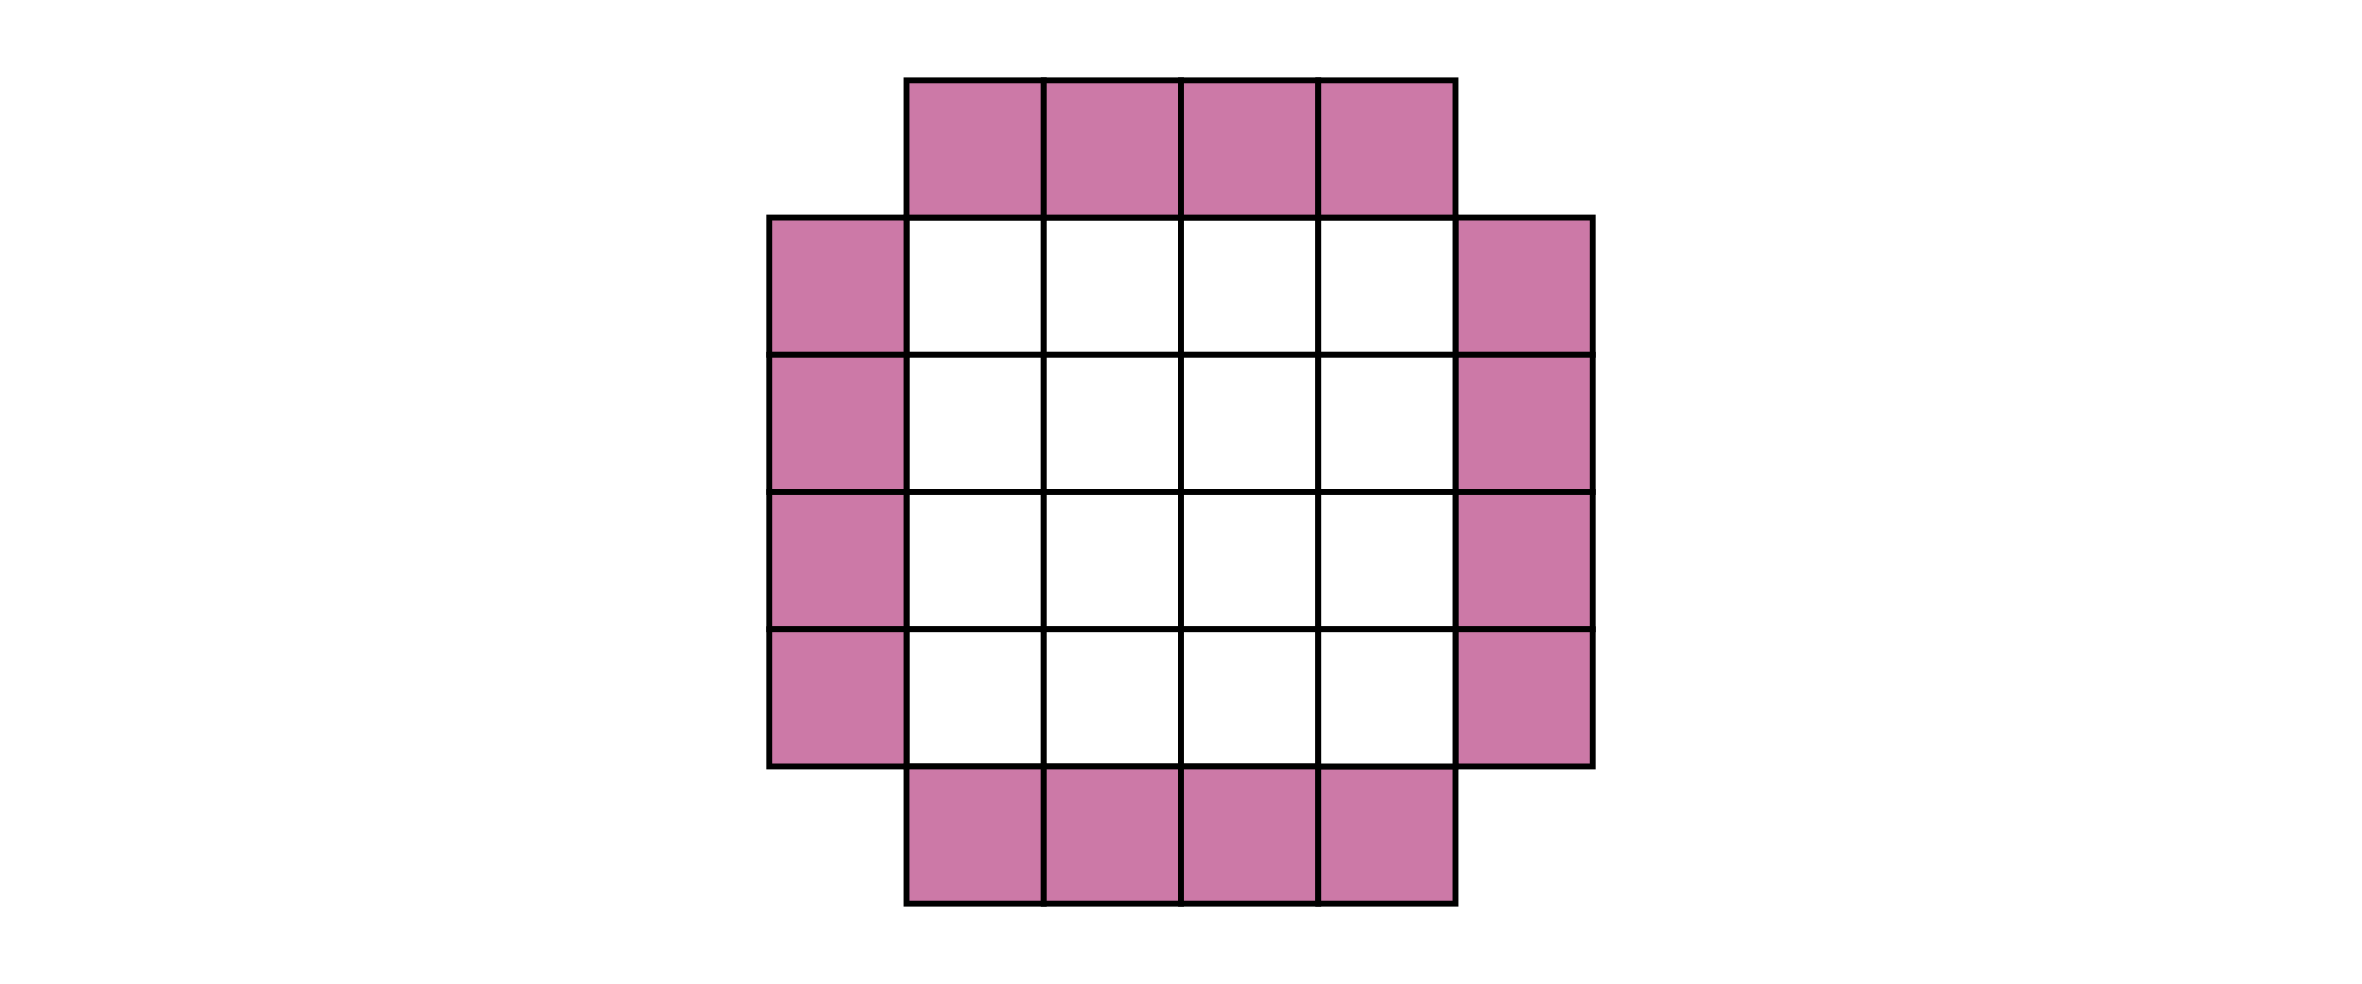
\includegraphics[width=\textwidth]{Figure 3.3.D}
\caption{The domain of a noise function operating upon a $4 \times 4$ system}
\end{figure}
Since cell values depend heavily depend on time and space for a generalized random walk, cannot simulate the true ``equilibrium state'' for Boolean random walks. The boundary noise function $W_t$ directly influences the asymptotic distribution of $X_t$ significantly more than the initial state $X_0$. We normally do not work with boundary noise functions for basic simulations.

The distribution of an countably-infinite time and countably-infinite space Boolean mechanical system has countably-infinite entropy at all time points. This is makes it impossible to simulate a truly infinite Boolean mechanical system, but a sufficiently large system would have the representation power to represent states of the observable universe. A study of more abstract physical systems can help us understand our reality at a more basic level.

\section{Boolean Random Walks}
\textbf{Boolean random walks}\index{Boolean random walk} are a generalization of random walks, and they are the fundamental tool for understanding Boolean mechanical systems. A Boolean mechanical system is a more general transition system, but it would be difficult to study due to a lack of physical intuition and motivation.
A Boolean random walk has a physical intuition via random walks and a computer science intuition by considering each particle-antiparticle as a \textit{bit flip}.

Let $X_t$ be a random walk with two classes from the set $\mathbb B_\pm = \{-1, +1\}$, and let $X_0$ be the initial configuration of the system. The system $X_t$ is a subset of the $d$-dimensional integer lattice $\mathbb Z^d$ with dimensional lengths $(n_1,...,n_d)$ for a total of:
$$\prod\limits_{i=1}^d n_i = N$$
entries or cells. If the element $\boldsymbol{+1}$ denotes a particle and there are $k$ particles, then there are $N-k$ antiparticles denoted $\boldsymbol{-1}$ in $X_t$. There are a total of:
$$\frac {N}{k! (N-k)!} = {N \choose k}$$
possible states with $k$ particles and $(N-k)$ antiparticles, and we denote this number of states as $\theta$.

The follwing is an example of a $2$-dimensional system $X_t$ with $8$ particles and $8$ antiparticles, and it has dimension lengths $(4,4)$ for a total of $4 \cdot 4 = 16$ cells:
\begin{figure}[H]
\centering
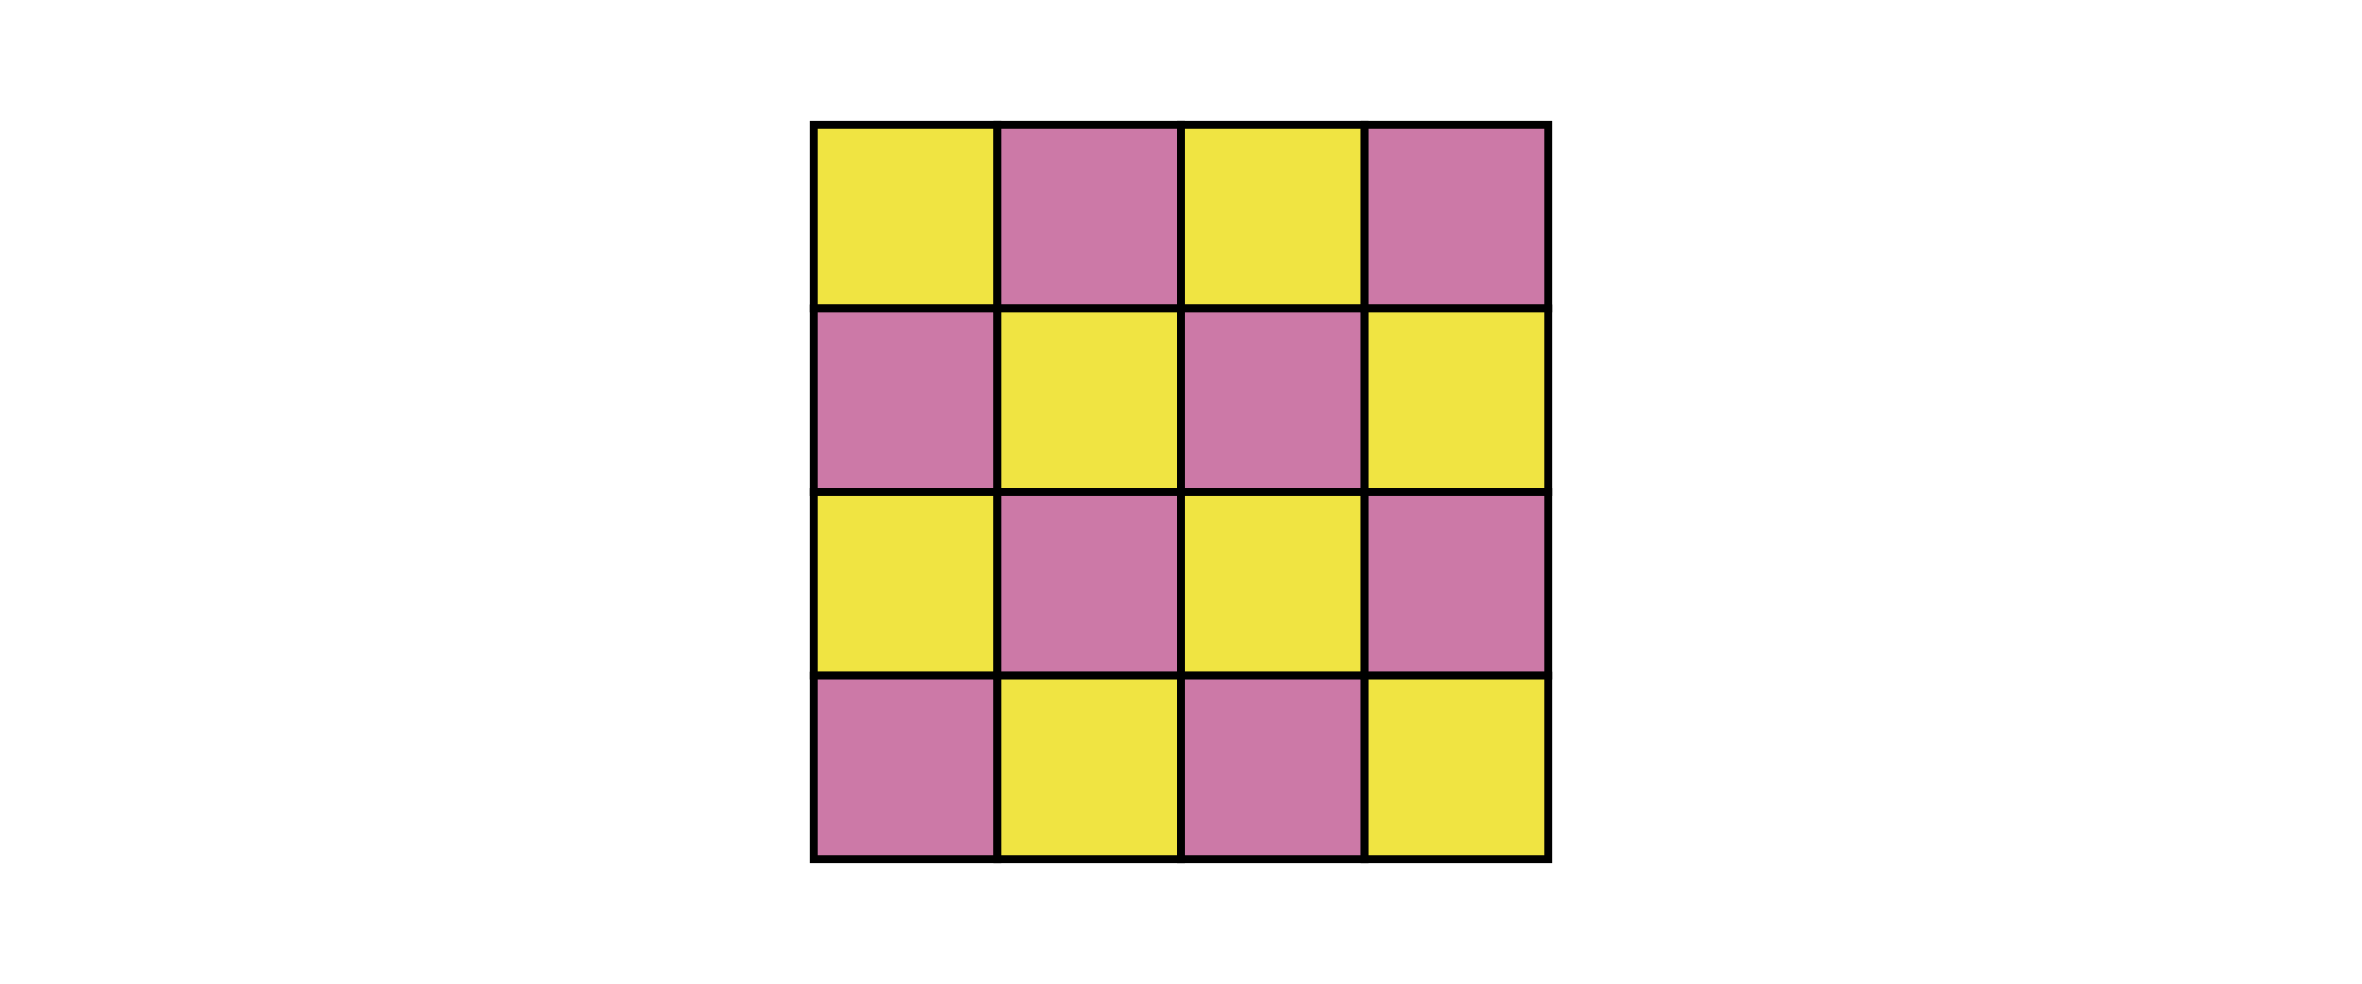
\includegraphics[width=\textwidth]{Figure 3.4.A}
\caption{A checkerboard state, high in process entropy}
\end{figure}
\noindent By default, we will be referring to $2$-dimensional systems due to their visual clarity on a page. When we observe the above Boolean mechanical system, it is unclear precisely how to handle the movement of particles that mirrors random walks.

Observe the following example systems $A_0$ and $B_0$:
\begin{figure}[H]
\centering
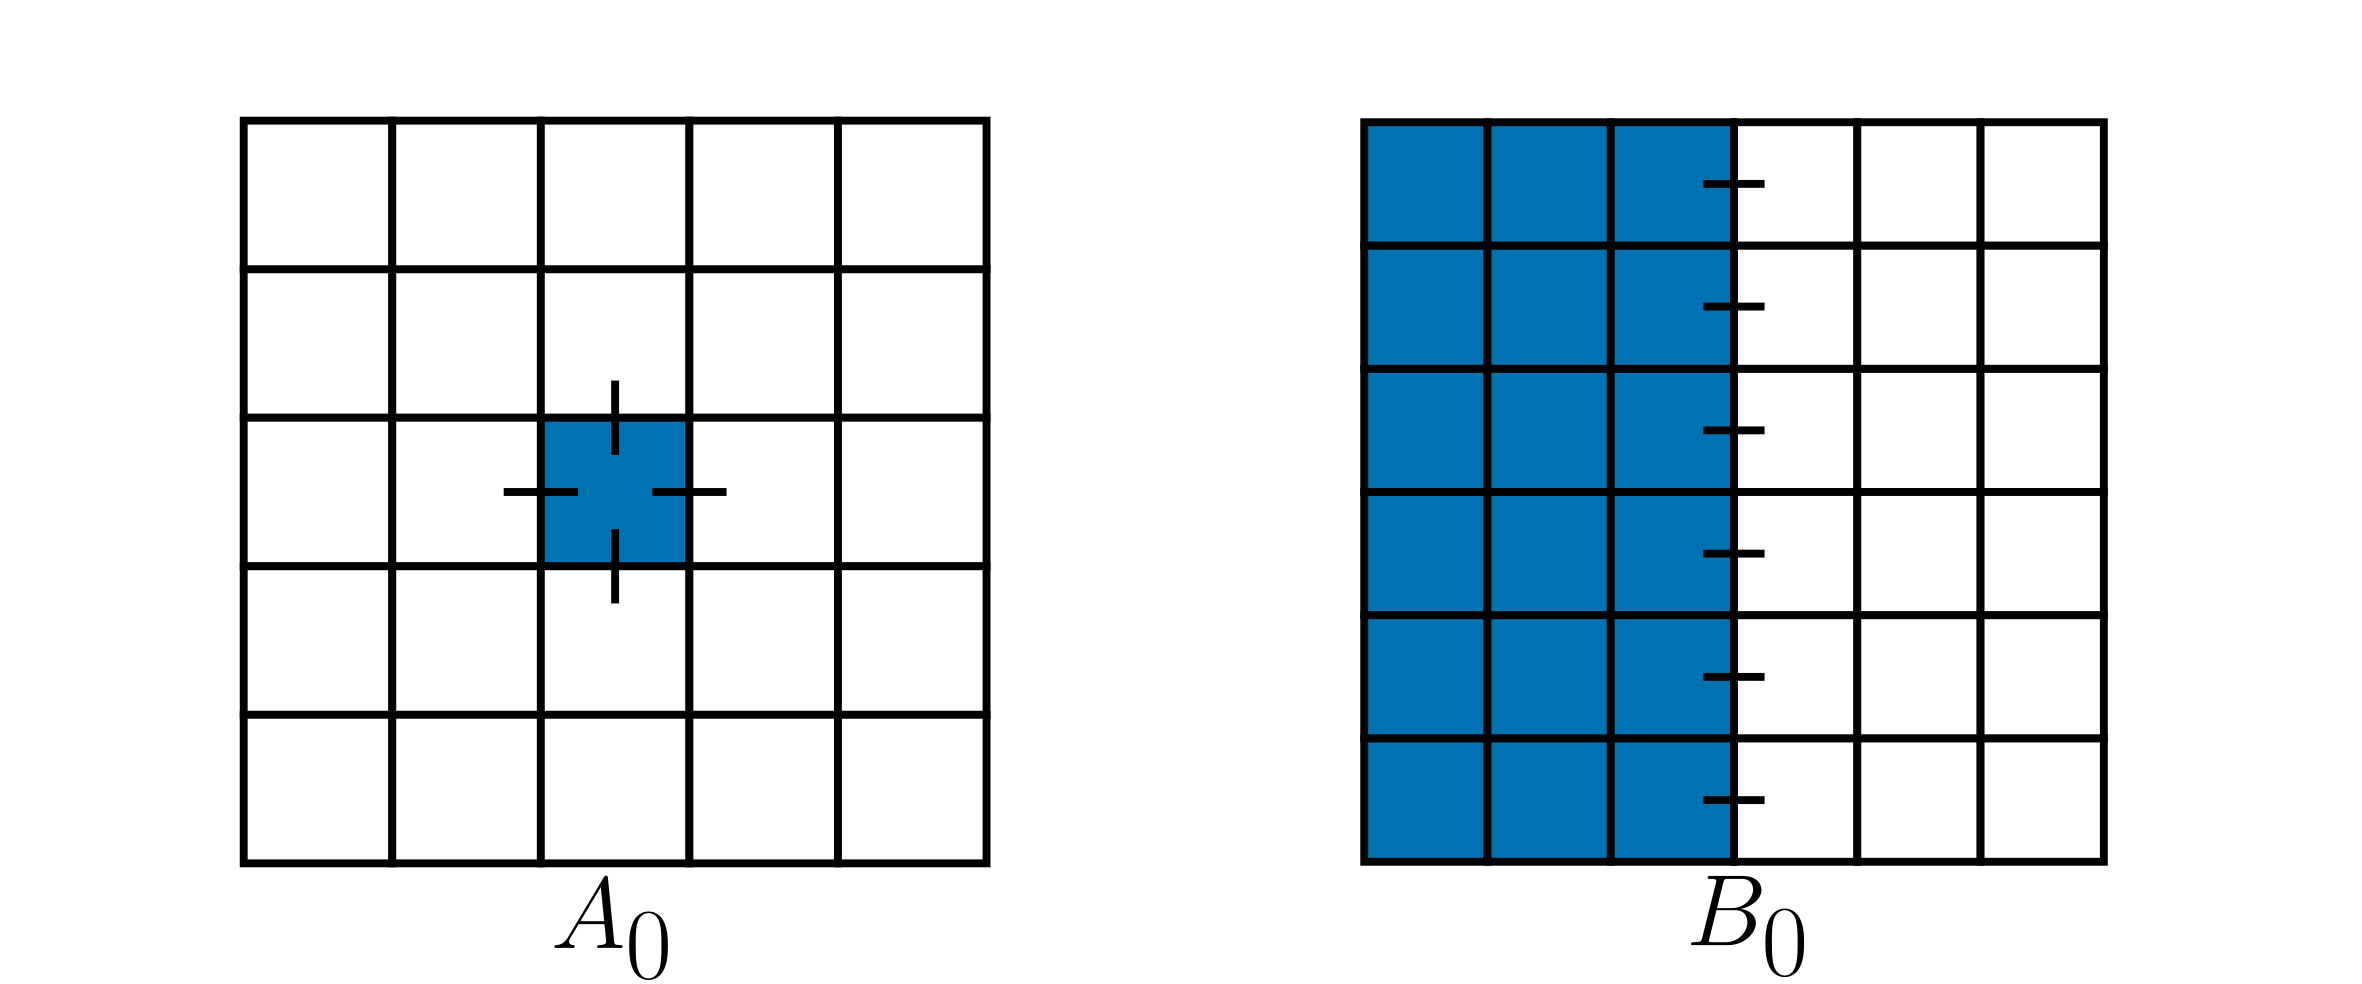
\includegraphics[width=\textwidth]{Figure 3.4.B}
\caption{Boolean states with ticks marking a spatial difference}
\end{figure}
\noindent The tick marks between cells denote where there is a difference in the Boolean value between cells. Therefore, a Boolean random walk evolves according to a \textit{stochastic binary differential equation}. It is vaguely reminiscent of the cellular automaton known as \textit{\S 5.2 Conway's Game of Life}.

The mathematics necessary to understand the depth of Boolean random walks is much larger than statistics alone. It requires dipping our toes into various seemingly disconnected topics in mathematics. Each topic is a branch of mathematics that is sufficiently complex to warrant its own set of textbooks and notation conventions. In order to understand the depth of Boolean mechanics, we must walk the breadth of topics under a unified notation. If you have sufficient background exposure to the topics covered in future chapters, skip to \textit{\S 9 Boolean Mechanical Systems}.

Returning to example system $A_0$, it is clear that $A_0$ imitates a $2$-dimensional simple random walk, though it is bounded to a finite set of cells. If you pay close attention, $A_0$ likewise has antiparticles blocked by antiparticles. Instead of perceiving filled spaces traveling through a void, we should interpret voids traveling through filled spaces as equally valid under the same rule. To understand Boolean random walks, we must erase our notion that space is empty and recognize that emptiness behaves like a fluid in its own right. If a random walk behaves like a fluid, so must its empty space. This property shall be referred to as \textbf{dichromatic symmetry}\index{dichromatic symmetry}.
\begin{figure}[H]
\centering
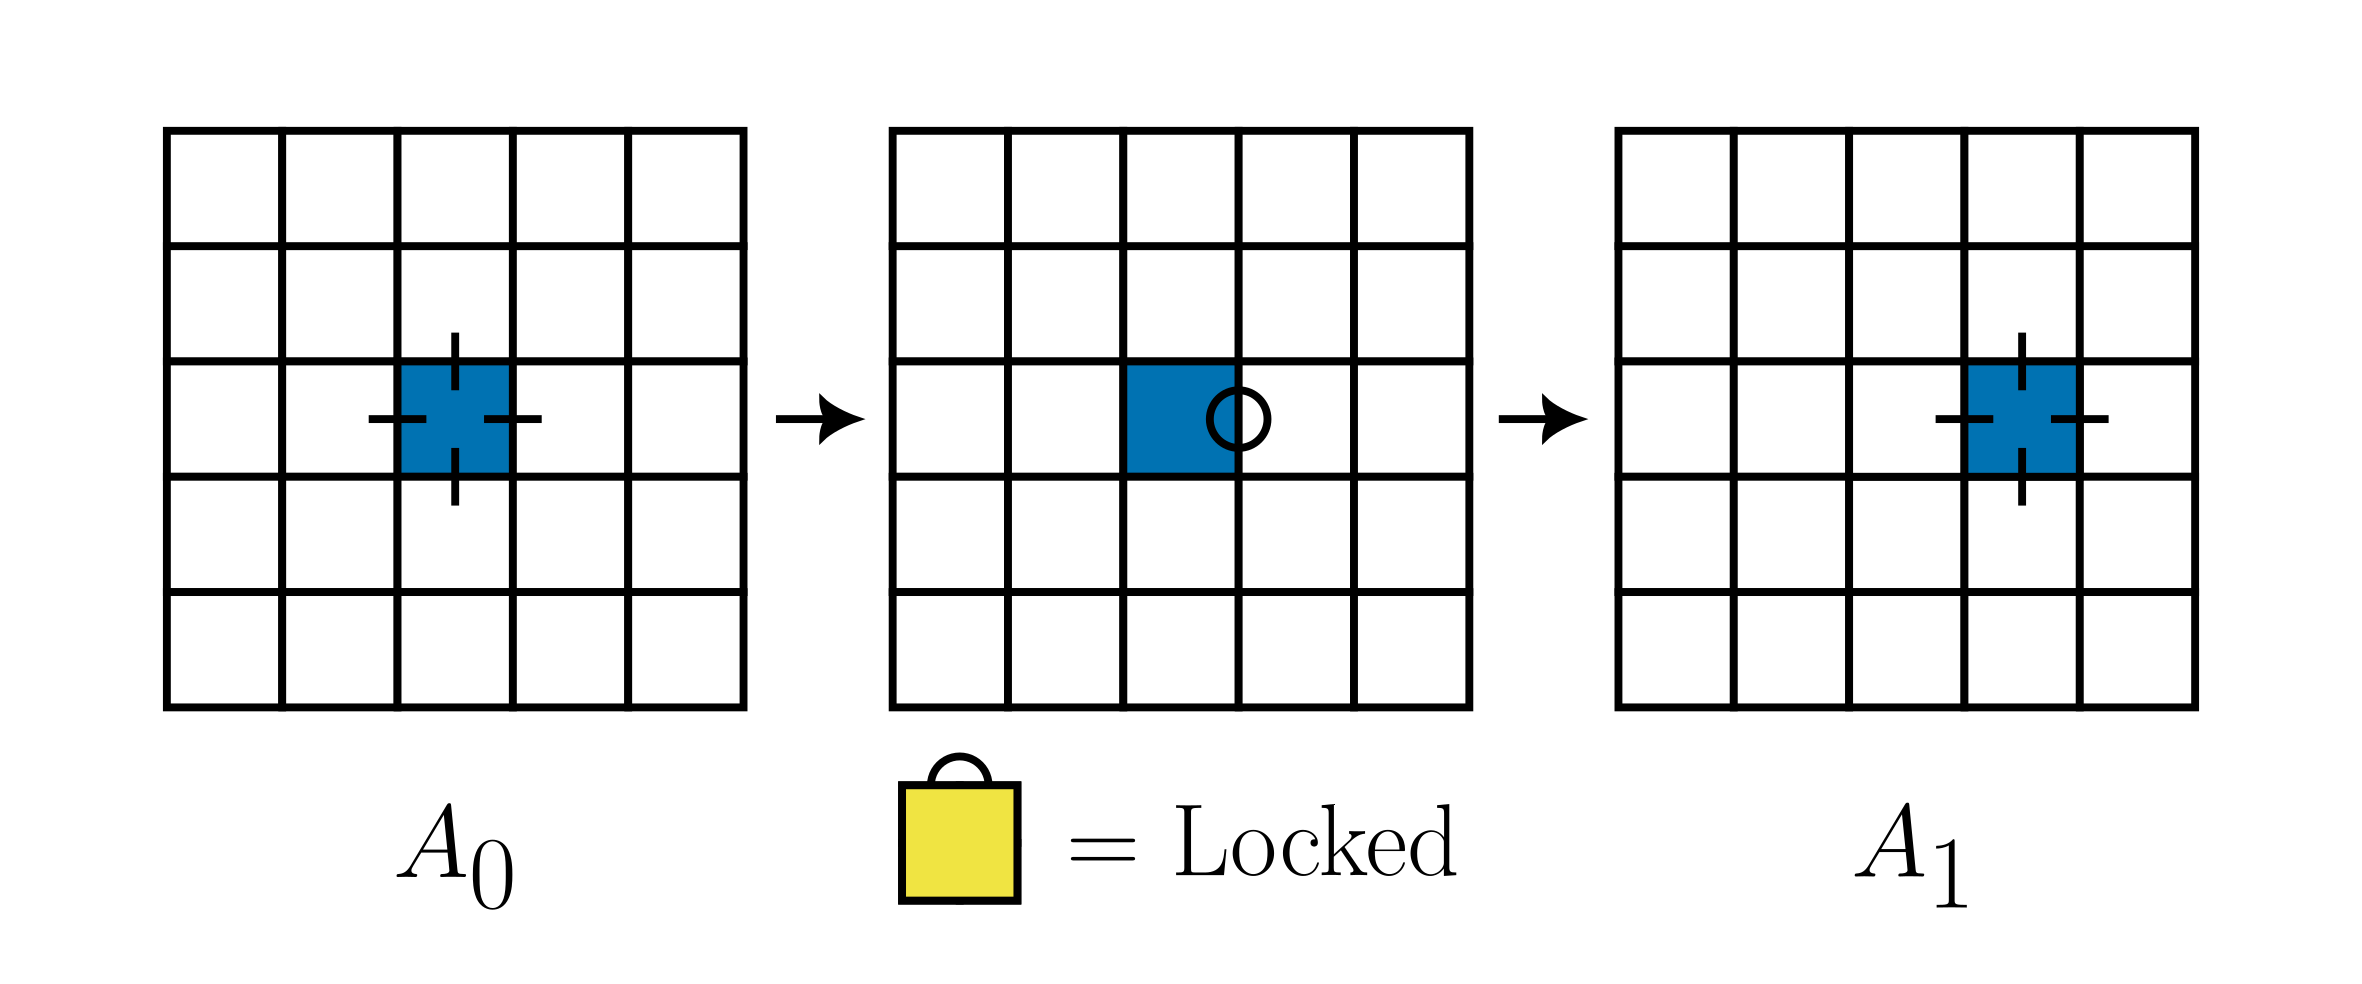
\includegraphics[width=\textwidth]{Figure 3.4.C}
\caption{A Boolean random walk transition denoted using ticks and circles. The circle represents a locked in bit flip between two cells, resembling a padlock.}
\end{figure}
\noindent In order to be computationally indistinguishable from a simple random walk, we must randomly sample valid differences, lock all cells marked to switch, then flip all cells marked to switch. If we allow a particle to double move, it is no longer a bisimulation of a random walk. In terms of cellular automata, it means it has exceeded the speed of light of $c=1$. 

With a firm grasp of the previous example systems in mind, we will define precisely what a system is.

\section{Boolean Dynamical Systems}
A \textbf{system}\index{system} $X_t$ is a single state that evolves to a new state over time, and each state $X$ is a tuple of values or labels $(x_1,...,x_N)$. The \textbf{state space}\index{state space} $\mathcal X = \{\hat X_1,...,\hat X_\theta \}$ is the set of all states that $X_t$ may evolve into in time. The probability measure of each future state $X_t$ is given by the probability function $\mu$, denoted as $\mu(X_t)$ or $\mu(X, t)$. The system's advancement in time is defined by some pushforward operator $\Lambda_\sharp$ on the measure $f$. A physical system is a tuple of values of in space that evolve over time. A Boolean mechanical system is a tuple of Boolean values in space and time, or this tuple $X$ is the Cartesian product of $N$ units of $x$.

Let $\Lambda$ be the pushforward of measure $\mu_1$ such that $\Lambda_{\sharp} \mu_1 = \mu_2$ is the \textbf{pushforward measure}\index{pushforward measure}. Let $\mu_1$ act on the measurable space $(X_1, \Sigma_1)$ and let $\mu_2$ act on the measurable space $(X_2, \Sigma_2)$. The pushforward of $\mu_1$ is defined by the following relation:
$$\mu_2 (E_2) = \Lambda_\sharp \mu_1 (E_2)= \mu_1 (\Lambda^{-1} E_2) = \mu_1 (E_1); E_1 \in \Sigma_1, \ E_2 \in \Sigma_2$$
If we think about what this means carefully, then the \textbf{transfer operator}\index{transfer operator} $\Lambda$ is implied to be related the eigenvalues of the system and $\Lambda_{\sharp} = e^{\frac{d}{d t}}$is the \textbf{shift operator}\index{shift operator} for time. The forward \textbf{shift operator}\index{shift operator} is defined like so:
$$e^{\tau \cdot \frac{d}{d t}}\mu (X,t) = \mu(X, t+\tau)$$
For iterative transfers, we say that $\Lambda$ may compose with itself: 
$$\Lambda ^ \tau = \underbrace{\Lambda \circ ... \circ \Lambda}_\text{$\tau$ times}$$
This iterated system closely ties to the ideas discussed in \textit{\S 8 Differential Equations}. 

We use the music sharp notation $\sharp$ to denote raising operations and the music flat notation $\flat$ to denote lowering operations. In this case $\Lambda_\flat = \Lambda_\sharp ^{-1}$ generates the \textbf{pullback measure}\index{pullback measure} of $\mu$. It directly follows that:
$$ \mu_2 (E_2) = \Lambda_\flat \mu_2(E_1) = \mu_1 (E_1) = \Lambda_\sharp \mu_1 (E_2) $$
from the relation:
$$\mu_1 (E_1) = \Lambda_\flat \mu_2(E_1) = \mu_2 (\Lambda E_1) = \mu_2 (E_2)$$
Simply put, $\mu_1$ is the pullback measure of $\mu_2$. Since we are often working systems that evolve from $t=0$, we may prefer the time-variable notation of $\mu_t(\Lambda^t E_0) = \mu_t (E_t)$. 

A \textbf{measure-preserving dynamical system}\index{measure-preserving dynamical system} is a $4$-tuple $(X, \Sigma, \mu, \Lambda)$ in which $X$ is a set, $\Sigma$ is a $\sigma$-algebra over $X$, $\mu$ is a probability measure, and $\Lambda$ is the transfer operator. If $E_t$ is an element of time-dependent $\sigma$-algebra $\Sigma_t$, then the pushforward measure:
$$\mu_{t+1}(E_{t+1}) = \Lambda_{\sharp} \mu_{t}(E_{t+1}) = e^{\frac{d}{dt}}\mu_t(E_{t+1}) = \mu_t(\Lambda^{-1} E_{t+1}) = \mu_t(E_t)$$
preserves the magnitude of the original probability measure of $E$. The basic idea is that for a given measure with magnitude $||\mu_t(E)||$, its future measure is also of the same magnitude $||\Lambda_{\sharp} \mu_t(E)|| = ||\mu_t(E)||$. Notice that the implicit time differential of the probability measure $\mu$ is given by:
$$\Lambda_\sharp = \frac{\mu_{t+1}(E_{t+1})}{\mu_t(E_t)}, \ \forall t \in \mathbb N$$
This is why we consider the transfer operator $\Lambda$ to be related the eigenvalues of the system, specifically an eigensystem of eigenvectors and eigenvalues. 

This idea of measure-preserving dynamical system is important when we are dealing with a stochastic transition matrix. Since our initial starting probability may differ, we need a rule that makes sure that probability is preserved even among different starting points. We discuss more about eigenvalues in \textit{\S 7.5 Transition Matrix}.

Let $\varepsilon_i$ be a unit $\sigma$-algebra of $x_i$. The \textbf{product $\sigma$-algebra}\index{product sigma algebra} of each set $\varepsilon_i$ is denoted as $\Sigma$. This $\Sigma$ is given by the Cartesian product:
$$\Sigma = \prod\limits_{i=1}^N \varepsilon_i$$
If each unit $x_i$ is an identical set $x_1 = ... = x_N$, then we call $x_i$ an measurable information unit and $X$ an information network. A prominent example is $x_i = \mathbb B_\pm = \{ -1, +1\}$, in which $X$ is a Boolean information network, or simply a Boolean network. Probability measures over some element $E$ of $\Sigma$ in which there exists some empty element, $\varepsilon_i = \varnothing$, are invalid while probability measures in which we use all elements, $\varepsilon_i = x_i$, sums over its unconditional probability. We may overlay this Boolean network over an ordered space, such as assigning an information unit over each element of the integer lattice $\mathbb Z^3$ such that $x_{ijk}$ refers to the measurable unit at integer coordinate $(i,j,k)$.

A \textbf{Boolean network}\index{Boolean network} has at most $2^N$ possible states in the state space $\mathcal X$. The probability measure of the system at time $t$ is given by $\mu(X_t)$, and it is given by the stochastic transition matrix $P: \mathcal X \rightarrow \mathcal X$. The \textbf{transition matrix}\index{transition matrix} $P$ denotes the probability that a state $\hat X_i$ becomes another state $\hat X_j$ in the Boolean network per unit of time:
$$P_{(i,j)} = \mu(\Lambda \hat X_i) = \mu(\hat X_j)$$
An attractor is a set of states that a system tends towards in time. An absorbing attractor is a single state that a system tends towards, and this creates a transient or degenerate system as all states will become this state. A state that you can only begin in but cannot reach through advancing time steps is called a \textit{garden-of-Eden state}. They are absorbing attractors in reversed time. Garden-of-Eden states do not occur in Boolean random walks. A further treatment of transition matrices given in \textit{\S 4.2 Markov Chains and Random Walks}, which are themselves tied to the idea of differential equations and \textit{Lie groups}. 

Diagonal matrices with elements from the set $\mathbb B_\pm = \{-1, +1\}$ are called \textbf{signature matrices}\index{signature matrix}. A system and its transitions may be described using a signature matrix. For example, two adjacent states in a $2 \times 2$ system are called $\hat X_i, \hat X_j$ in the stochastic matrix $P$. Written in diagonal form, they have a product equal to their quotient:
$$\textnormal{diag}(\hat X_i) =\begin{bmatrix}
+1 & 0 & 0 & 0 \\
0 & -1 & 0 & 0 \\
0 & 0 & -1 & 0 \\
0 & 0 & 0 & +1
\end{bmatrix}$$

$$\textnormal{diag}(\hat X_j)=\begin{bmatrix}
-1 & 0 & 0 & 0 \\
0 & +1 & 0 & 0 \\
0 & 0 & +1 & 0 \\
0 & 0 & 0 & -1
\end{bmatrix}
$$
$$
\textnormal{diag}(\hat X_i) \times \textnormal{diag}(\hat X_j) = \frac{\textnormal{diag}(\hat X_i)}{\textnormal{diag}(\hat X_j)} = 
\begin{bmatrix}
-1 & 0 & 0 & 0 \\
0 & -1 & 0 & 0 \\
0 & 0 & -1 & 0 \\
0 & 0 & 0 & -1
\end{bmatrix}
$$
that must have a of determinant $1$. This means transitions between states isomorphic to some subset of the \textit{special linear group} $\textnormal{SL}(\mathbb N, 2)$. This text does not describe Lie groups and Lie algebras in detail, but it is suffice to say that Lie groups whose elements are computable numbers are of the utmost interest to Boolean mechanics.

\section{Generalized Random Walks}
Generalized random walks are an extension of the binary classes of $\mathbb B_\pm = \{-1,+1\}$ to any number of classes with weight matrix $\omega$. Observe the following weight matrix for the Boolean set:
$$\omega_{\mathbb B} = 
\begin{bmatrix}
0 & 1 \\
1 & 0
\end{bmatrix}
$$
\noindent
Notice how particles may only exchange with antiparticles and that $\omega_{\mathbb B}$ is symmetric along the main diagonal. We require that $\omega$ be symmetric along the main diagonal in general. All entries of the weight matrix $\omega$ must be greater than or equal to $0$, therefore $\omega$ is a positive semi-definite matrix.

The following example weight matrix $\omega_3$ has three classes $\{a,b,c\}$ in which the third class $c$ may switch with itself:
$$\omega_{3} = 
\begin{bmatrix}
0 & 1 & 1 \\
1 & 0 & 1 \\
1 & 1 & 1
\end{bmatrix}
$$
This means that class $c$ has a tendency to cluster around itself. In a more abstract sense, you might say that macroscopic patterns of $\omega_{\mathbb B}$ with this tendency also tend to cluster since they prefer to gravitate towards themselves. The class has more mass, and this idea of self-preference and self-gravitation is important for theories in physics such as loop quantum gravity.

The following example weight matrix $\omega_5$ is quite exotic since some classes have more weighted switches and some cannot switch at all:

$$\omega_{5} = 
\begin{bmatrix}
0 & 1 & 0 & 1 & 0 \\
1 & 1 & 2 & 0 & 0 \\
0 & 2 & 1 & 1 & 0 \\
1 & 0 & 1 & 1 & 0 \\
0 & 0 & 0 & 0 & 0
\end{bmatrix}
$$
We call this non-switching class with weight $0$ a \textit{wall}, similar to how a bounded random walk has reflecting walls. The classes with higher weights tend to switch first. More valid switches and more weight on switches means they are chosen more often, and this means they lock out other classes more frequently.

\section{Random Walks in Higher Dimensions}
Random walks in higher dimensions than $d=2$ have a key property discovered by George P\'{o}lya: they are not guaranteed to return where they started even when given infinite time. In $d=1$ and $d=2$, the probability of recurrence is $1$. The probability of recurrence $P(d)$ of a random walker in $d$ dimensions is given by the following relations:
$$P(d) = 1 - \frac{1}{Q(d)}$$
$$Q(d) = \int\limits_0^\infty I(0, \frac{t}{d})^d e^{-t} dt$$
in which $I(\alpha, t)$ is the modified Bessel function of the first kind as discussed in \textit{\S Diffusion and Heat Equation}.

Normally when we are performing a simulation of Boolean random walks, we are working with a bounded simulation that imitates gas particles in a box. With an infinite space and infinite time Boolean random walk simulation, we cannot guarantee that Boolean random walkers will interact in the future for $d \geq 3$. This is perhaps the main flaw of Boolean random walks as a possible theory of a computable universe, but this is easily fixed by introducing random noise to the final state of each cell. From then, the \textbf{word problem}\index{word problem} means it is undecidable if two equally powerful theories of a computational universe can map any two representations between them.

\chapter{Stochastic Processes}
\section{Motivations for Learning Stochastic Processes}
Good jazz, like good weather, is dances the line between order and chaos. The most interesting things in the world are comprehensible, yet they elude our ability to understand and predict them. As humanity succeeds in forecasting the motions of the world, it gains the power to reshape it in new ways. In order to see how the world really works, we must escape the cave in Plato's allegory.

A \textbf{stochastic process}\index{stochastic process} models how a set of states randomly evolves over time. In a sense, stochastic processes are fundamental to understanding how our uncertain world works. The roiling of waves, the passage of clouds, the motion of stars, and sparks of the mind. These natural phenomena evade precise explanation with words because they are not deterministic processes. 

In response to this randomness, nature's creations have sensors for things that do not say the same: light, heat, sound, and more. Life can be hard to predict in general, yet each life form must gain control over its limiting resources in order to survive. Even if an event is approximately deterministic, it may have so many moving parts that it is functionally random to a small mind.

In order to understand the world, the mind flitters between thoughts using algorithms both deterministic and stochastic. Both but not truly one or the other. The creative part of the mind aimlessly generates new ideas while the logical part ruthlessly cuts them with words and labels. One neuron sparks another by mere chance, but it was them being connected that made that chance possible, inevitable, in the first place.

Despite all the recurring patterns and sequences such as the temperature of the seasons and the clouds before rain, a single drop of rain in the clear skies of fall noon may kiss you on the forehead. That is the eureka moment that set me on the path to writing this book. Our mathematics and physics may allow us to predict when the sun will die, but we can scarcely predict when and how it will become a star anew in the future. The distance too vast, the variables too many, our minds too small. At the very least, stochastic processes let us accurately describe small Boolean mechanical systems.

\section{Markov Chains and Random Walks}
A \textbf{Markov chain}\index{Markov chain} is a model of stochastic processes with a countable number of states. A \textbf{stochastic process}\index{stochastic process} is a random variable denoted using $X_t$, and it begins at time $t=0$. This random variable assumes a value from the set of possible states at each time step. The \textbf{state space}\index{state space} $\mathcal X = \{\hat X_1,...,\hat X_\theta\}$ is set of all states relevant to the Markov chain, and the total number of states is given by the cardinality $|\mathcal X| = \theta$. The \textbf{transition matrix}\index{transition matrix} $P_{\theta \times \theta}$ indicates a set of transition probabilities between elements of the state space. The \textbf{Markov property}\index{Markov property} states that the probability distribution for a future state only depends on the current state. The \textbf{state vector}\index{state vector} $y_t$ represents the ordered set of probabilities that the system is in at time $t$ upon the state space $\mathcal X$. 

A simple bounded random walk with $5$ cells in 1D is visualized like so at time $t=0$:
\begin{figure}[H]
\centering
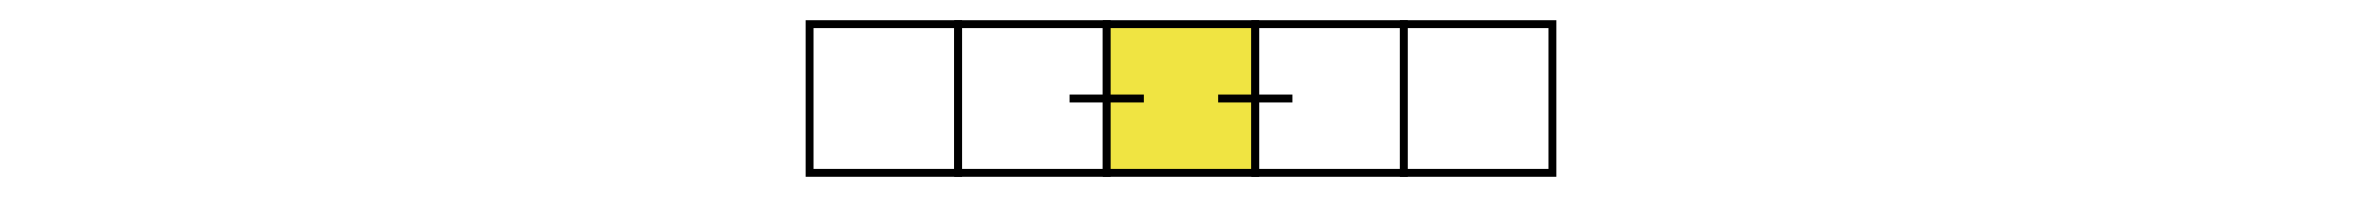
\includegraphics[width=\textwidth]{Figure 4.2.A}
\caption{A bounded random walker upon $5$ cells in $1$-dimension}
\end{figure}
There are clearly only $5$ states that this system can be in. Coincidentally, the state vector $y_0$ is modeled in parallel as:
$$y_0 = [0 \ 0 \ 1 \ 0 \ 0]$$
We may enumerate our entire state space $\mathcal X = \{\hat X_1,\hat X_2,\hat X_3, \hat X_4, \hat X_5\}$ with a proper visualization of transition probabilities in the following way:
\begin{figure}[H]
\centering
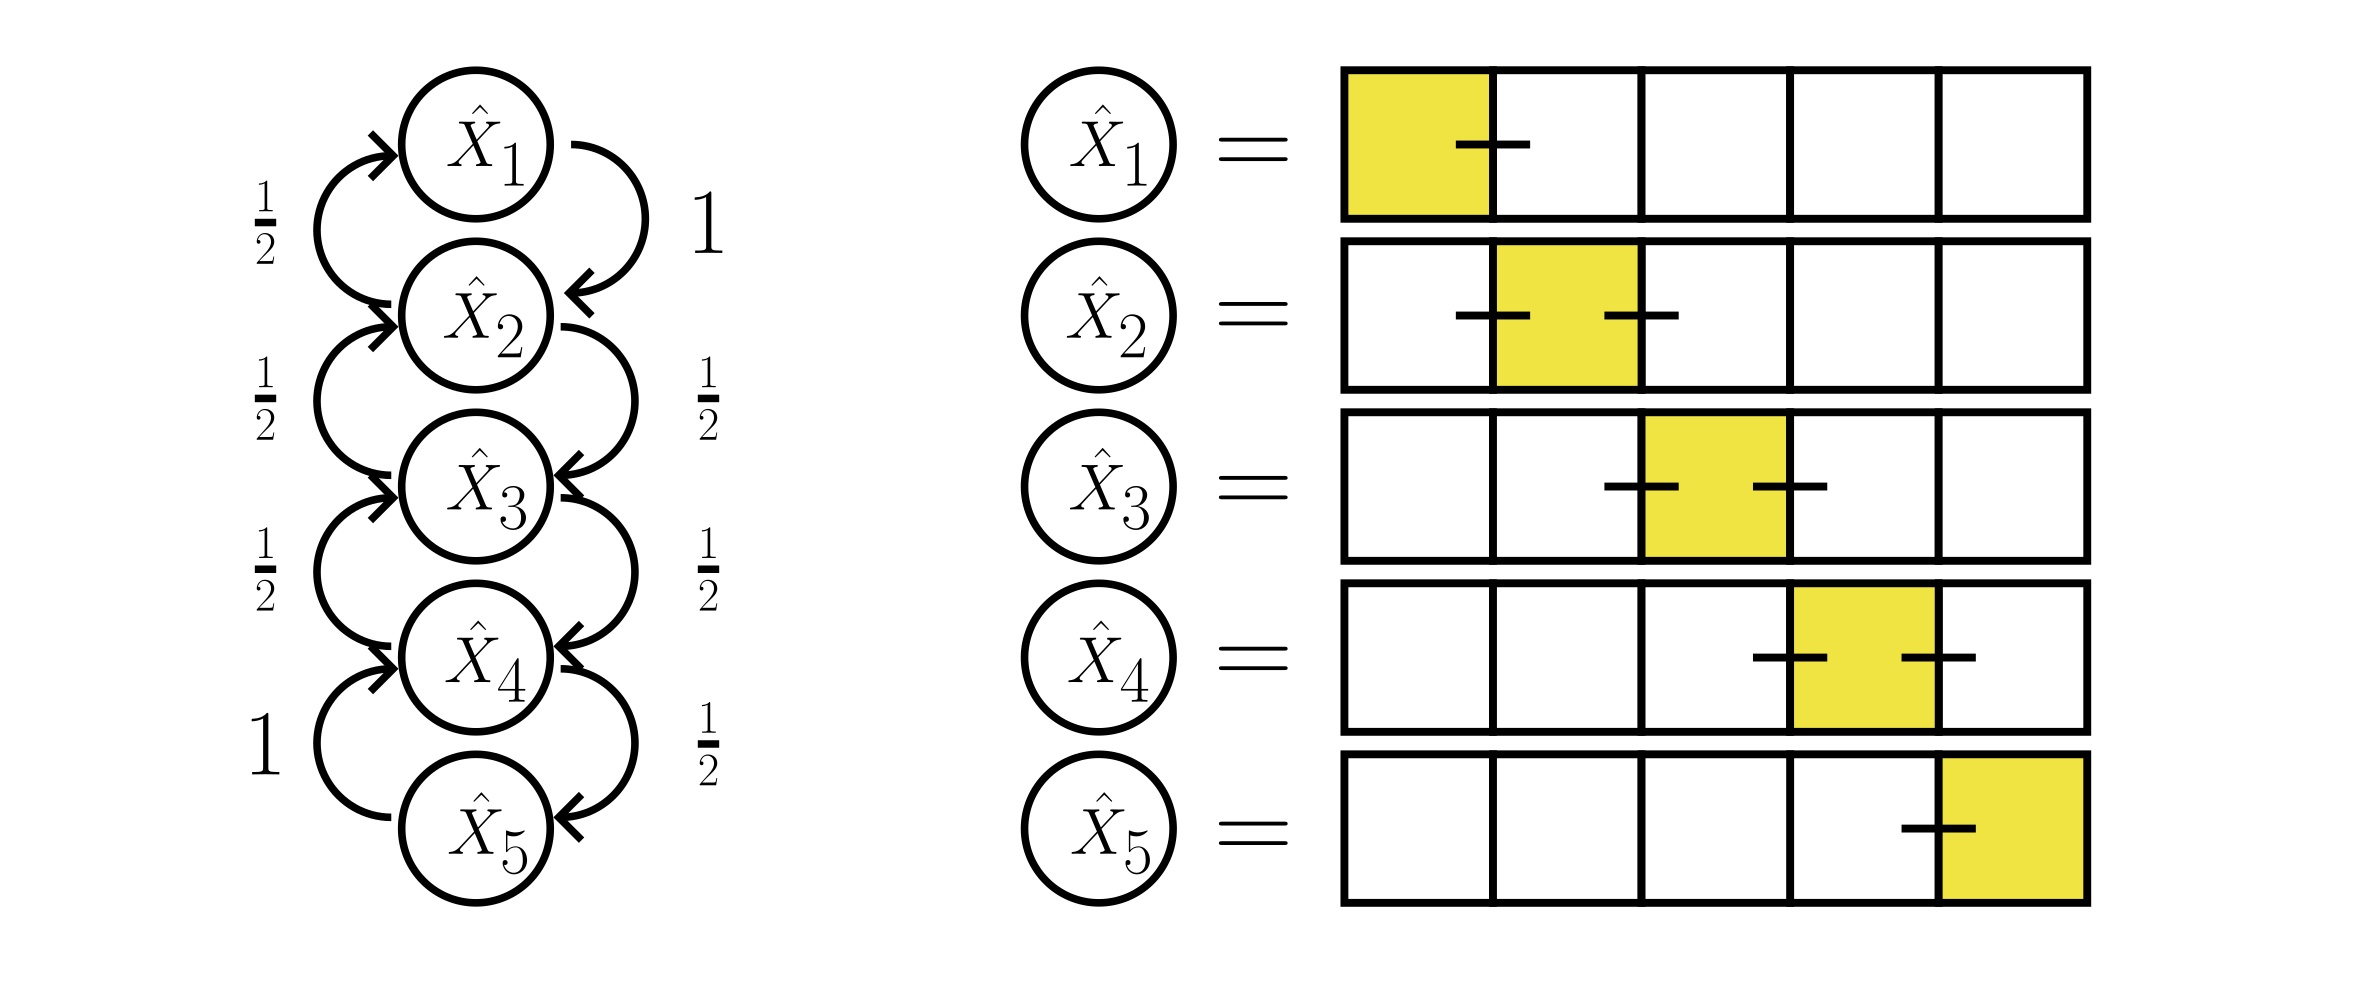
\includegraphics[width=\textwidth]{Figure 4.2.B}
\caption{The Markov chain representing the $5$ states of our random walker}
\end{figure}
Notice that this means our specific system $X$ at time $0$, $X_0$, is in the 3-rd state with probability 1. Since the particle has an equal probability of moving left or right except at the edge, the stochastic matrix $P$ is:
$$P = 
\begin{bmatrix}
0 & 1 & 0 & 0 & 0 \\
\frac{1}{2} & 0 & \frac{1}{2} & 0 & 0 \\
0 & \frac{1}{2} & 0 & \frac{1}{2} & 0 \\
0 & 0 & \frac{1}{2} & 0 & \frac{1}{2} \\
0 & 0 & 0 & 1 & 0
\end{bmatrix}
$$
We define $P_{(i,j)}$ as the probability that state $\hat X_i$ transitions into state $\hat X_j$ after one unit of time has passed.\footnote{Most matrix notation indicates rows and columns using $P_{ij}$ instead of $P_{(i,j)}$ . My matrix notation helps specify dimensionality and subsetting such as $A_{(i \in I, j \in J, k \in K)}$. This is most useful when programming.} We require that each row's probability sums to $1$:
$$\sum\limits_{j=1}^\theta P_{(i, j)} = 1, \quad \forall i \in \{ 1,...,\theta \}$$
in order to obey Kolmogorov's axioms of probability per state. This row-column convention is called a right-stochastic matrix, and this convention defines left eigenvectors such that $v P = \lambda P$ for eigenvector $v$ and its eigenvalue $\lambda$. In contrast, the more common linear algebra right eigenvector convention defines $P v = P \lambda$.

Any stochastic process with a countable number of states may be modeled as a Markov chain using a stochastic transition matrix. In practice, only stochastic processes with a finite number of states $\theta < \infty$ can be simulated on a computer using state vector $y$ and stochastic matrix $P$. We hit the machine epsilon limit of a computer rather quickly if we try to make a stochastic process model of the weather.

It is also worth noting that a Markov chain is effectively a bounded random walk on a state space graph. See sections \textit{\S 3.3 Bounded Random Walk} to review bounded random walks and \textit{\S 7.4 Adjacency Matrix} to learn more about the connectedness of state spaces $\mathcal X$.

If system $X_t$ is represented using state vector $y_t$, then $P^s = P \times ... \times P$ represents the transition matrix after $s$ time steps such that:
$$y_t P^s = y_{t+s}$$
in which $y_{t+s}$ is the probability distribution of states for the system $X_{t+s}$. The $s$-th power of $P$, $P^s$, gives the $s$-step transition probability such that:
$$(P^s)_{(i, j)} = P(X_{t+s} = \hat X_j | X_{t} = \hat X_i)$$
defines the conditional probability that a system in state configuration $\hat X_i$ at time $t$ is in state configuration $\hat X_j$ at time $t+s$. This is what we meant by the Markov property as the future system configuration distribution for $X_{t+s}$ only depends on the system current configuration $X_{t}$. More specifically, this memoryless property means the probability only depends on the \textit{most recent} information.

A pair of states are said to \textit{communicate} if both have a path by which each may reach the other. A Markov chain is said to have $n$ \textit{communication classes} if there are $n$ sets of Markov chains that may be separated, or reduced, into $n$ non-communicating Markov chains. The transition probability across communication classes is zero. A Markov chain is said to be \textit{irreducible} if it has precisely one communication class. The following is an abstract representation of the reducibility of a stochastic matrix $P$ with $3$ communication classes:
\begin{figure}[H]
\centering
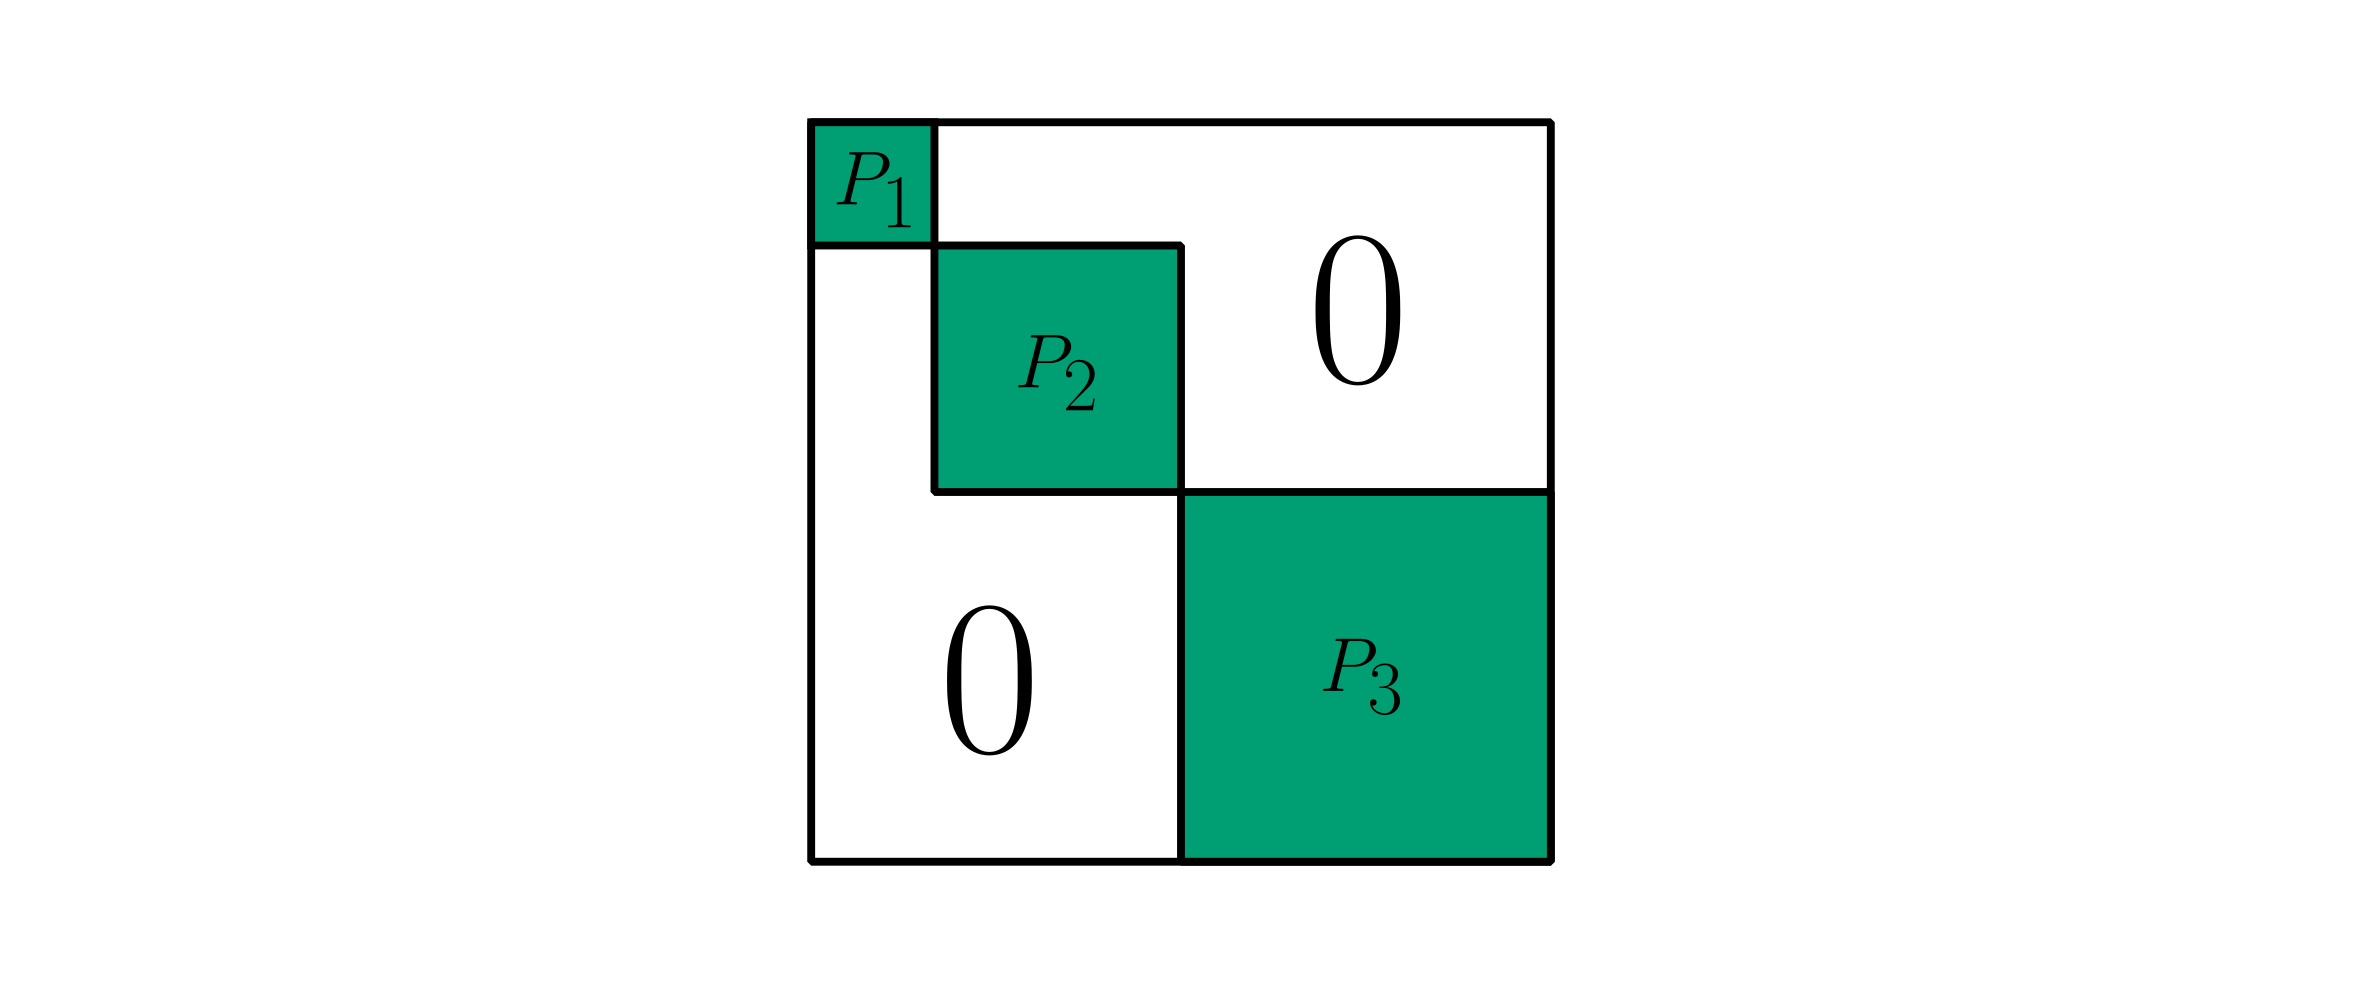
\includegraphics[width=\textwidth]{Figure 4.2.C}
\caption{A stochastic matrix $P$ with three communication classes}
\end{figure}
\noindent
Note how an $n$-class Markov chain's transition matrix may be constructed from $n$ irreducible transition matrices. We discuss the the idea of ``weak communication'' across communication classes in \textbf{\S Appendix D: Class Stochastic Matrices}.

A state configuration $\hat X_i$ is said to be \textbf{recurrent}\index{recurrent state} if it is guaranteed to return to itself in the future, and a state $\hat X_i$ is instead said to be \textbf{transient}\index{transient state} if there is a non-zero probability of never returning to itself in the future. The expected hitting time for a state $\hat X_i$ to return to itself is given by:
$$\mathrm{E}(T_i) = \sum\limits_{t=1}^\infty t \cdot (P^t)_{ii}$$
If the expected return time is finite, $\mathrm{E}(T_i) < \infty$, then state $\hat X_i$ is \textbf{positive recurrent}\index{positive recurrent}. Else if $\mathrm{E}(T_i) = \infty$, then $\hat X_i$ is \textbf{null recurrent}\index{null recurrent}. A state $\hat X_i$ is said to be \textbf{absorbing}\index{absorbing state} if there are no outgoing transition from the state, $\mathrm{E}(T_i) = 1$. 

Recall that a state in a communication class will never transition outside of its current communication class. These recurrence properties apply to the entire communication class. A single state is positive recurrent if and only if its communication class is positive recurrent. A single state is null recurrent if and only if its communication class is null recurrent.

A state $\hat X_i$ is said to be $\boldsymbol n$\textbf{-periodic}\index{$n$-periodic states} if it always takes at least $n$ transitions to return to itself. A communication class is said to be $\boldsymbol n$\textbf{-periodic} \index{$n$-periodic class} if it always takes at least $n$ transitions for each state in the class to return to itself. A Boolean random walk is always $2$-periodic if $\textnormal{min}(k, N-k) \geq 1$. Closely related is the idea of state \textbf{parity}\index{parity}: Odd states may only transition to even states, and even states may only transition to odd states. A $1$-periodic system is alternatively called \textit{aperiodic}. A Markov communication class is said to be \textbf{ergodic}\index{ergodic} if its is recurrent and aperiodic.

A stochastic transition matrix $P$ is said to be \textbf{dichromatically symmetric}\index{dichromatic symmetry} if it is a permutation of another stochastic matrix $A$, and $A$ is a stochastic matrix that is symmetric about a $180^\circ$ rotation:
$$A = 
\begin{bmatrix}
A_{(1, 1)} & A_{(1, 2)} & \cdots & \cdots & A_{(1, \theta-1)} & A_{(1, \theta)} \\
A_{(2, 1)} & A_{(2, 2)} & \cdots & \cdots & A_{(2, \theta-1)} & A_{(2, \theta)} \\
\vdots & \vdots & \ddots & \ & \vdots & \vdots\\
\vdots & \vdots & \ & \ddots & \vdots & \vdots\\
A_{(\theta-1, 1)} & A_{(\theta-1, 2)} & \cdots & \cdots & A_{(\theta-1, \theta-1)} & A_{(\theta-1, \theta)} \\
A_{(\theta, 1)} & A_{(\theta, 2)} & \cdots & \cdots & A_{(\theta, \theta-1)} & A_{(\theta, \theta)} 
\end{bmatrix}
$$
If we rotate $A$ by $180^\circ$, then we ensure that the $(\theta-k)$-th row is a reversal of the $k$-th row:
$$A = \begin{bmatrix}
A_{(\theta, \theta)} & A_{(\theta, \theta-1)} & \cdots & \cdots & A_{(\theta, 2)} & A_{(\theta, 1)} \\
A_{(\theta-1, \theta)} & A_{(\theta-1, \theta-1)} & \cdots & \cdots & A_{(\theta-1, 2)} & A_{(\theta-1, 1)} \\
\vdots & \vdots & \ddots & \ & \vdots & \vdots\\
\vdots & \vdots & \ & \ddots & \vdots & \vdots\\
A_{(2, \theta)} & A_{(2, \theta-1)} & \cdots & \cdots & A_{(2, 2)} & A_{(2, 1)} \\
A_{(1, 1)} & A_{(1, 2)} & \cdots & \cdots & A_{(1, \theta-1)} & A_{(1, \theta)} 
\end{bmatrix}
$$
It is easy to verify dichromatic symmetry for a Boolean mechanical system in the transition matrix. If the state space represents a linear Boolean sequence such as:
$$\mathcal X = (000, 001, 010, 011, 100, 101, 110, 111)$$
then we want the transition probabilities of Boolean inverses to obey this row reversal property. We use the set $\mathbb B_\circ = \{0, 1\}$ for convenience.

The most obvious example of a Boolean mechanical system state $\hat X$ and its Boolean inverse is the checkerboard state:
\begin{figure}[H]
\centering
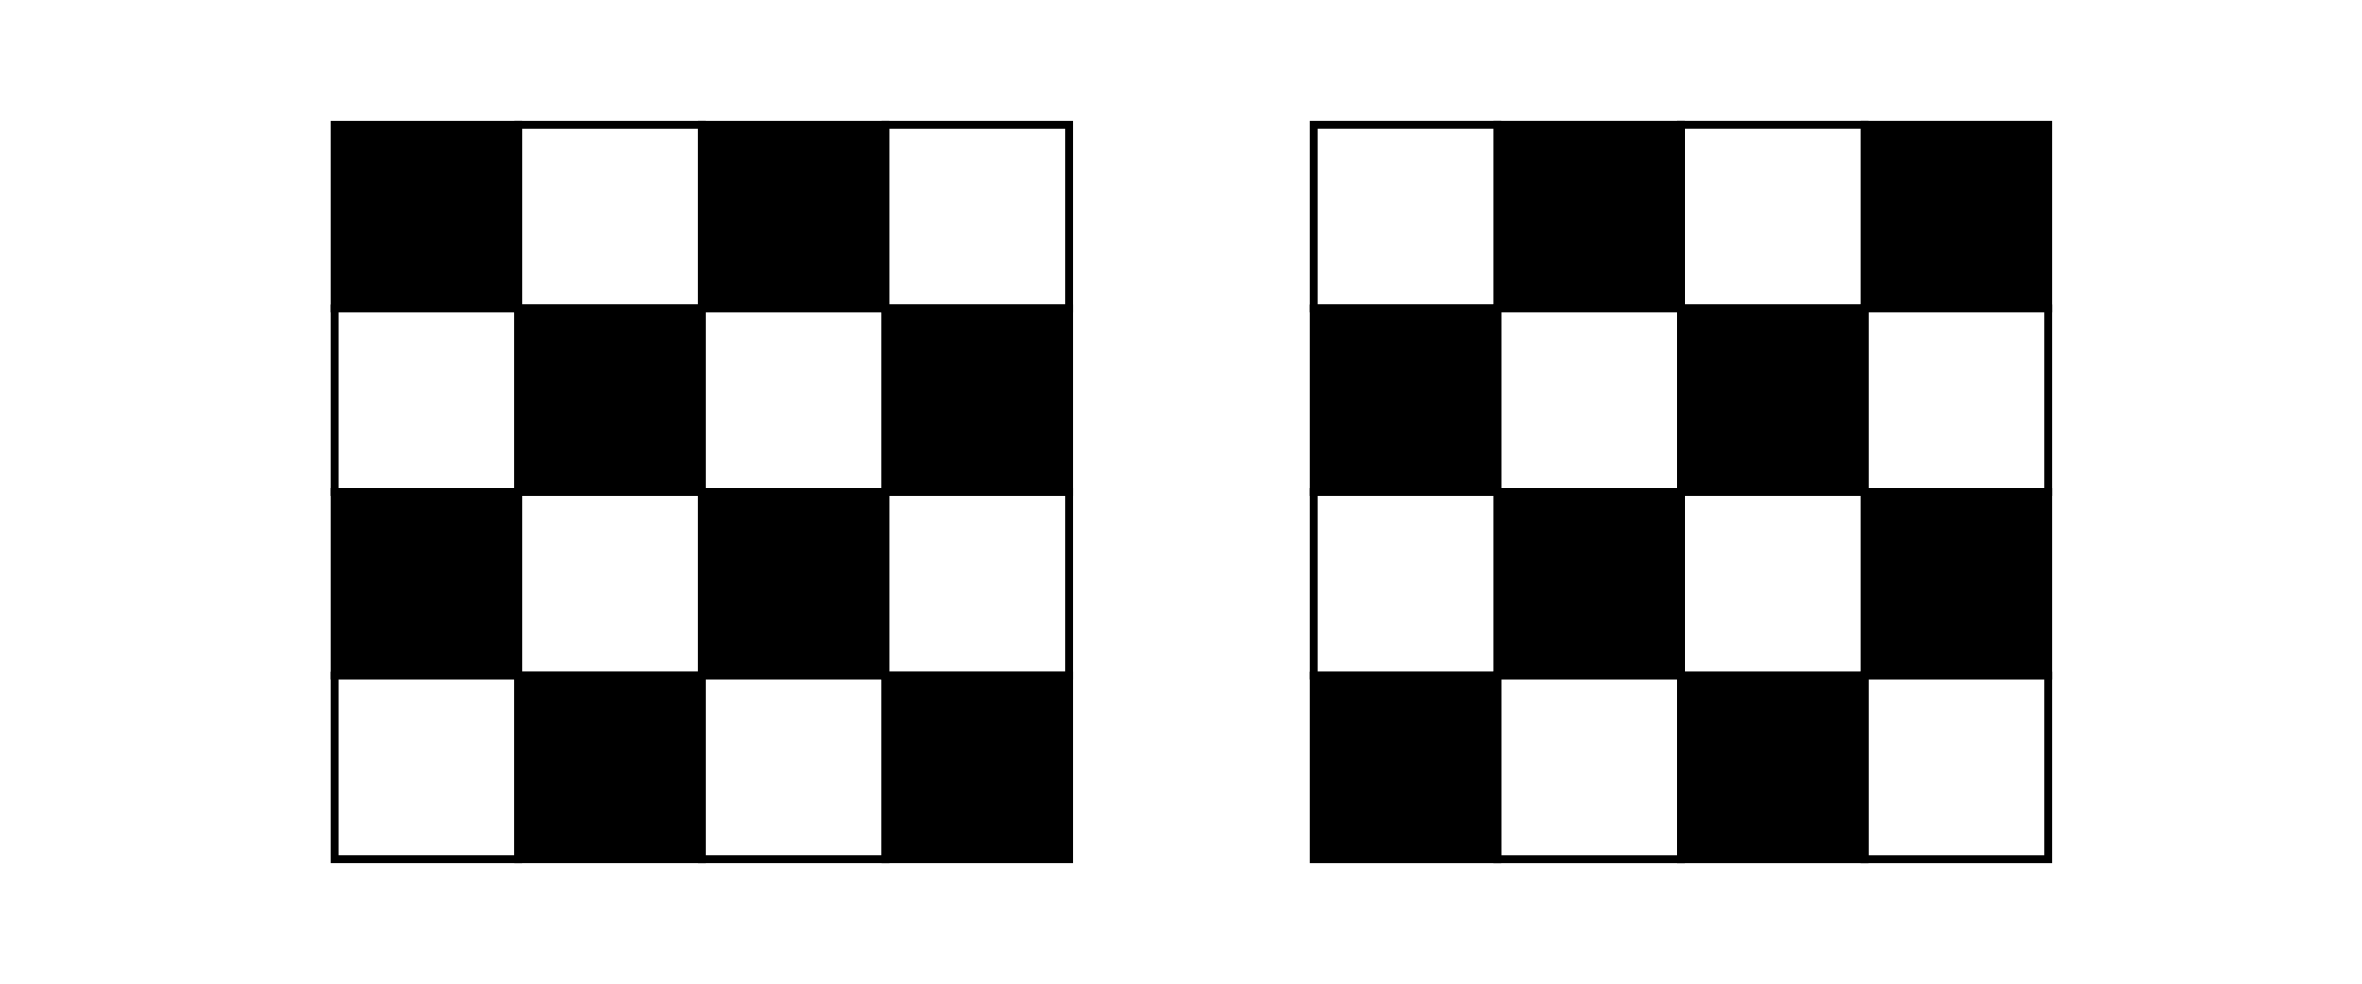
\includegraphics[width=\textwidth]{Figure 4.2.D}
\caption{The two checkerboard states have high process entropy}
\end{figure}
\noindent
which may transition into each other and are in the same communication class. We may index a state with a natural number by multiplying each cell $x_i$ by $2^i$
$$\textnormal{index}(\hat X) = \bigg [ \sum\limits_{i=1}^N (2^i)x_i) \bigg ] - 1$$
in which the value of each cell $x$ is using the Boolean set $\mathbb B_\circ = \{0, 1\}$.

\section{Poisson Processes for Large Volumes}

The \textbf{Poisson distribution}\index{Poisson distribution} represents the probability distribution of the arrival of a discrete count of objects over a continuous time:
$$f(x) = \frac{\lambda ^x e^{-\lambda}}{x!}, \quad x \in \mathbb N, \lambda \in \mathbb R^+$$
The Poisson distribution is the limiting case of the Binomial distribution:
$$f(y) = {t \choose y} p^y (1-p)^{t-y}, \ y \in \{0,1,...,t\}, \ p \in [0,1]$$
for continuous time $t$ in which $\mathrm{E}(X) = \mathrm{E}(Y)$. The Poisson distribution is a better description for stochastic processes involving rare events per unit of time. In the case of Boolean mechanical systems, some sets of system state configurations are so rare that the discreteness of time and space is a trivial factor. For example, the planar separated state:
\begin{figure}[H]
\centering
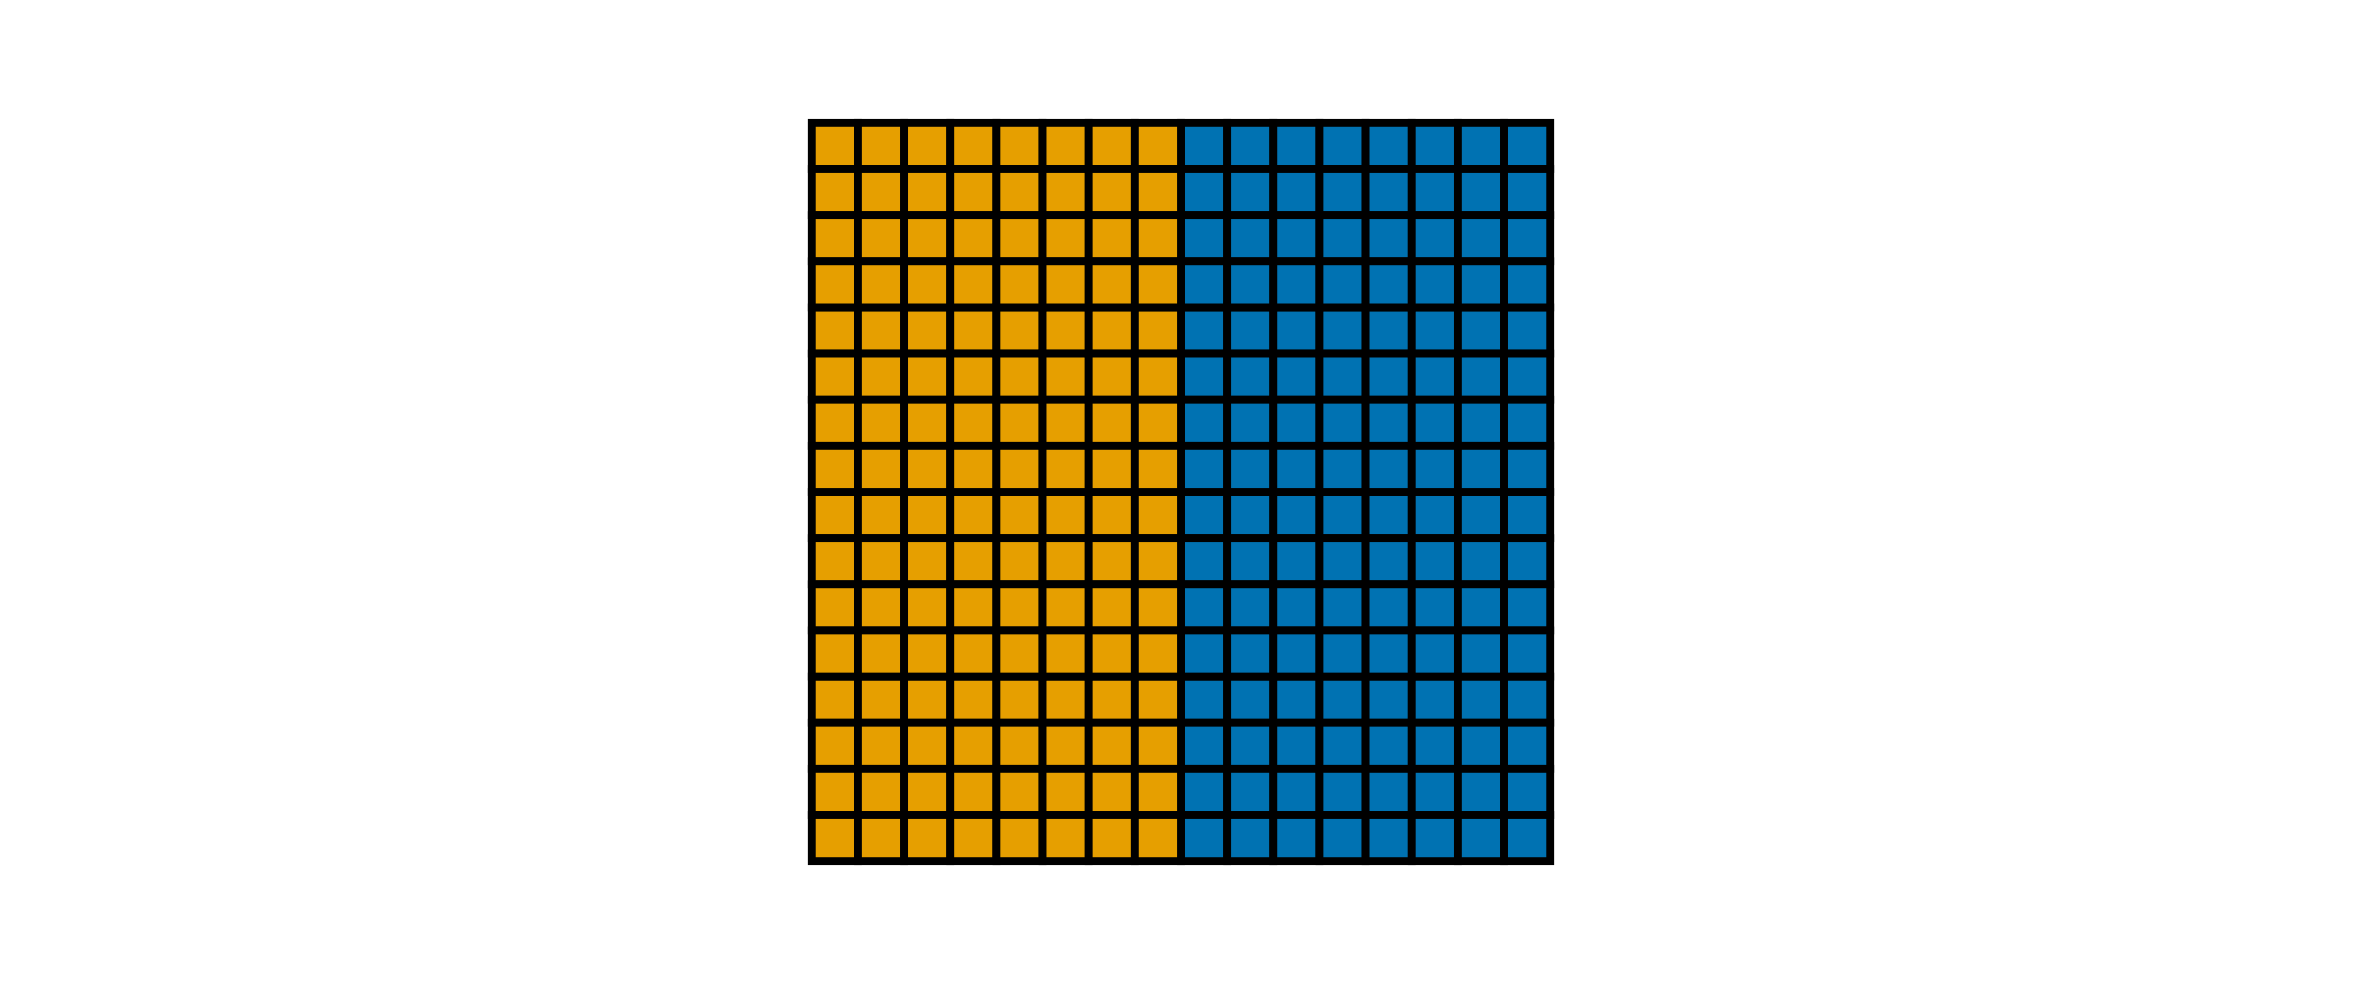
\includegraphics[width=\textwidth]{Figure 4.3.A}
\caption{Planar patterns are unlikely as a subset of a larger pattern}
\end{figure}
\noindent 
is an extremely rare configuration for a larger Boolean random walk simulation to contain in its subsets.

Suppose that $G \sim \textnormal{Poisson}(V \cdot \lambda)$ in which $V$ is the overall volume of the search for the state $\gamma$ (or the set of states $\Gamma$ of the same volume) with frequency rate $\lambda$ per $1$ unit volume. We use $G$ to denote the probability distribution of the arrival of \textbf{logic gates}\index{logic gate}, more specifically \textbf{random logic gates} in Boolean mechanical systems. When we are working with large systems such as a cube of volume $V = 1000^3$ in which some collection of states $\Gamma$ is quite rare, then a Poisson process model of:
$$f_G(g) \approx\frac{(V \cdot \lambda)^g e^{-V \cdot \lambda}}{g!} , \quad g \in \mathbb N $$
is a good model for predicting how often any state $\gamma \in \Gamma$ occur. 

Let $X$ be a cubic region that may or may not contain $\gamma$ in $\Gamma$. If states $\gamma$ in $\Gamma$ are not rare such that the cubic samples $X$ have:
$$f(X \in \Gamma) < \frac{1}{V}$$
then the expectation and variance in frequency is low since $\mathrm{E}(G) = V \cdot \lambda$ and $\mathrm{Var}(G) = V \cdot \lambda$. In other words, if a cubic sample $X$ has a probability of containing an element of $\Gamma$ is greater than the inverse volume, then it may not be rare enough to use a Poisson process to describe its arrival using a continuous approximation. We prefer the existence probability to be lower than the contribution of a pixel of the volume. We call this \textbf{subpixel probability}\index{subpixel probability} requirement, and it eases the memoryless property that a Poisson process normally requires to be homogeneous.

When we describe a Poisson process, we assume that the spatial distribution of $\gamma \in \Gamma$ is either independent or rare enough to be homogeneous. \textbf{Inhomogeneous Poisson processes}\index{inhomogeneous Poisson process} are Poisson processes that have an underlying spatial dependence such that the frequency $\lambda$ is a function of coordinate vector $\boldsymbol x = (x_1,...,x_d)$. We call $\lambda(\boldsymbol x)$ the \textbf{intensity function}\index{intensity function} of the arrival rate.

For a Boolean random walk, we don't know the true spatial dependence of cubic sample $X$, and the conditional dependence occurs all the way down to the scale of individual Boolean cells. The following illustration describe the importance of rarity $\lambda$ relative to volume $V$:
\begin{figure}[H]
\centering
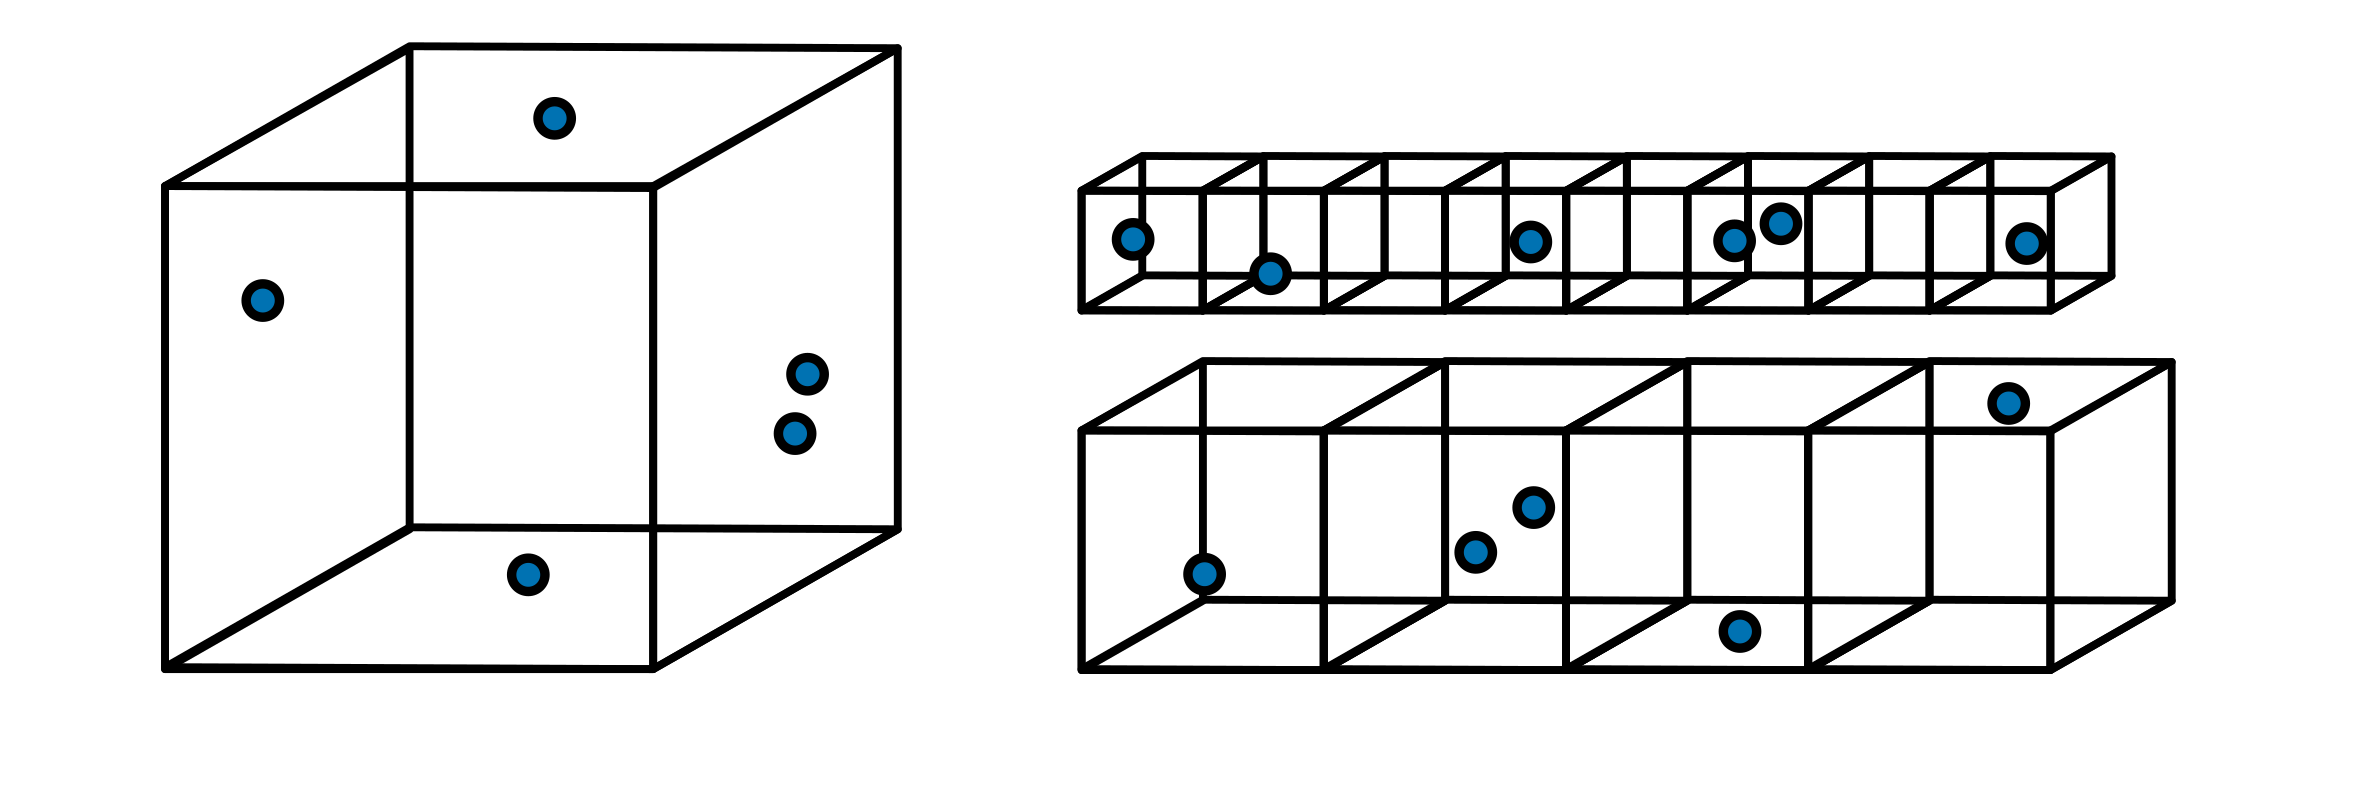
\includegraphics[width=\textwidth]{Figure 4.3.B}
\caption{Volume determines Poisson process sensitivity to spatial dependence}
\end{figure}
\noindent
Supposing some desired logic gates $\gamma \in \Gamma$ are extremely rare rare, it is unlikely that the spatial dependence will matter when describing the spatial process $G$. For example, the spatial dependence of stars due to gravity and interaction is inconsequential to the spatial distribution due to their overall rarity per volume of space. Thus, the stars are approximately distributed according to a Poisson process, even though stars obviously cluster into galaxies due to gravity.

Of particular interest are states that are rare yet statistically stable. We go into further detail about the stability of a set of states $\Gamma$ in \textit{\S 10 Macroscopic Behavior}.

\section{Brownian Motion and Martingales}

\textbf{Brownian motion}\index{Brownian motion} describes the physical process of the motion of particles suspended in a fluid, and the motion is described mathematically as a \textbf{Wiener process}\index{Wiener process}. The fluid may be a gas, a liquid, or similar. The particle may be any object influenced by the fluid, including identical fluid particles, non-identical fluid particles, or even empty space. In a cup of water, physical particles may be subject to buoyancy and gravity, but empty space requires zero modification to the theory to account for these influences. The motion of empty space essentially describes a massless particle.

The spaces between $k$ particles are assumed to be so large that the probability of collision of two or three particles occupying the same space is inconsequentially small. If two 3D random walkers start at the origin with initial time probability distribution:
$$f(\boldsymbol 0,0) = 1$$
 for each, the probability that they attempt to occupy the same space at time $t$ is given by $f(\boldsymbol x, t)^2$. A Wiener process is the continuum limit of a random walk, or rather a random walk is a finite approximation of a Wiener process's infinite fractal path. This means that the Wiener process $W_t$ is continuous everywhere but differentiable nowhere.

A \textbf{martingale}\index{martingale} is a stochastic process in which the expected value of the future always equals the previous time step:
$$\mathrm{E}(X_{t+1} | X_1,...,X_t) = \mathrm{E}(X_{t+1} | X_t) = X_t$$
This property is true for both random walks and Wiener processes. It is a special case of the Markov property with extra the extra constraint that the expected value is itself the value previous state.

\section{Random Fields}
A \textbf{random field}\index{random field} is a stochastic process in which a field of values at time $t=0$ evolves over time and space randomly. The initial random field is called $X_0$, and the random field at time $t$ is $X_t$. The probability distribution on the possible field of values is called $f(x,t)$. A simple random field is the Bernoulli random field on $\mathbb Z^2$ in which each cell randomly chooses a value from the Boolean set $\mathbb B_\pm = \{-1, +1\}$ at each time step.
\begin{figure}[H]
\centering
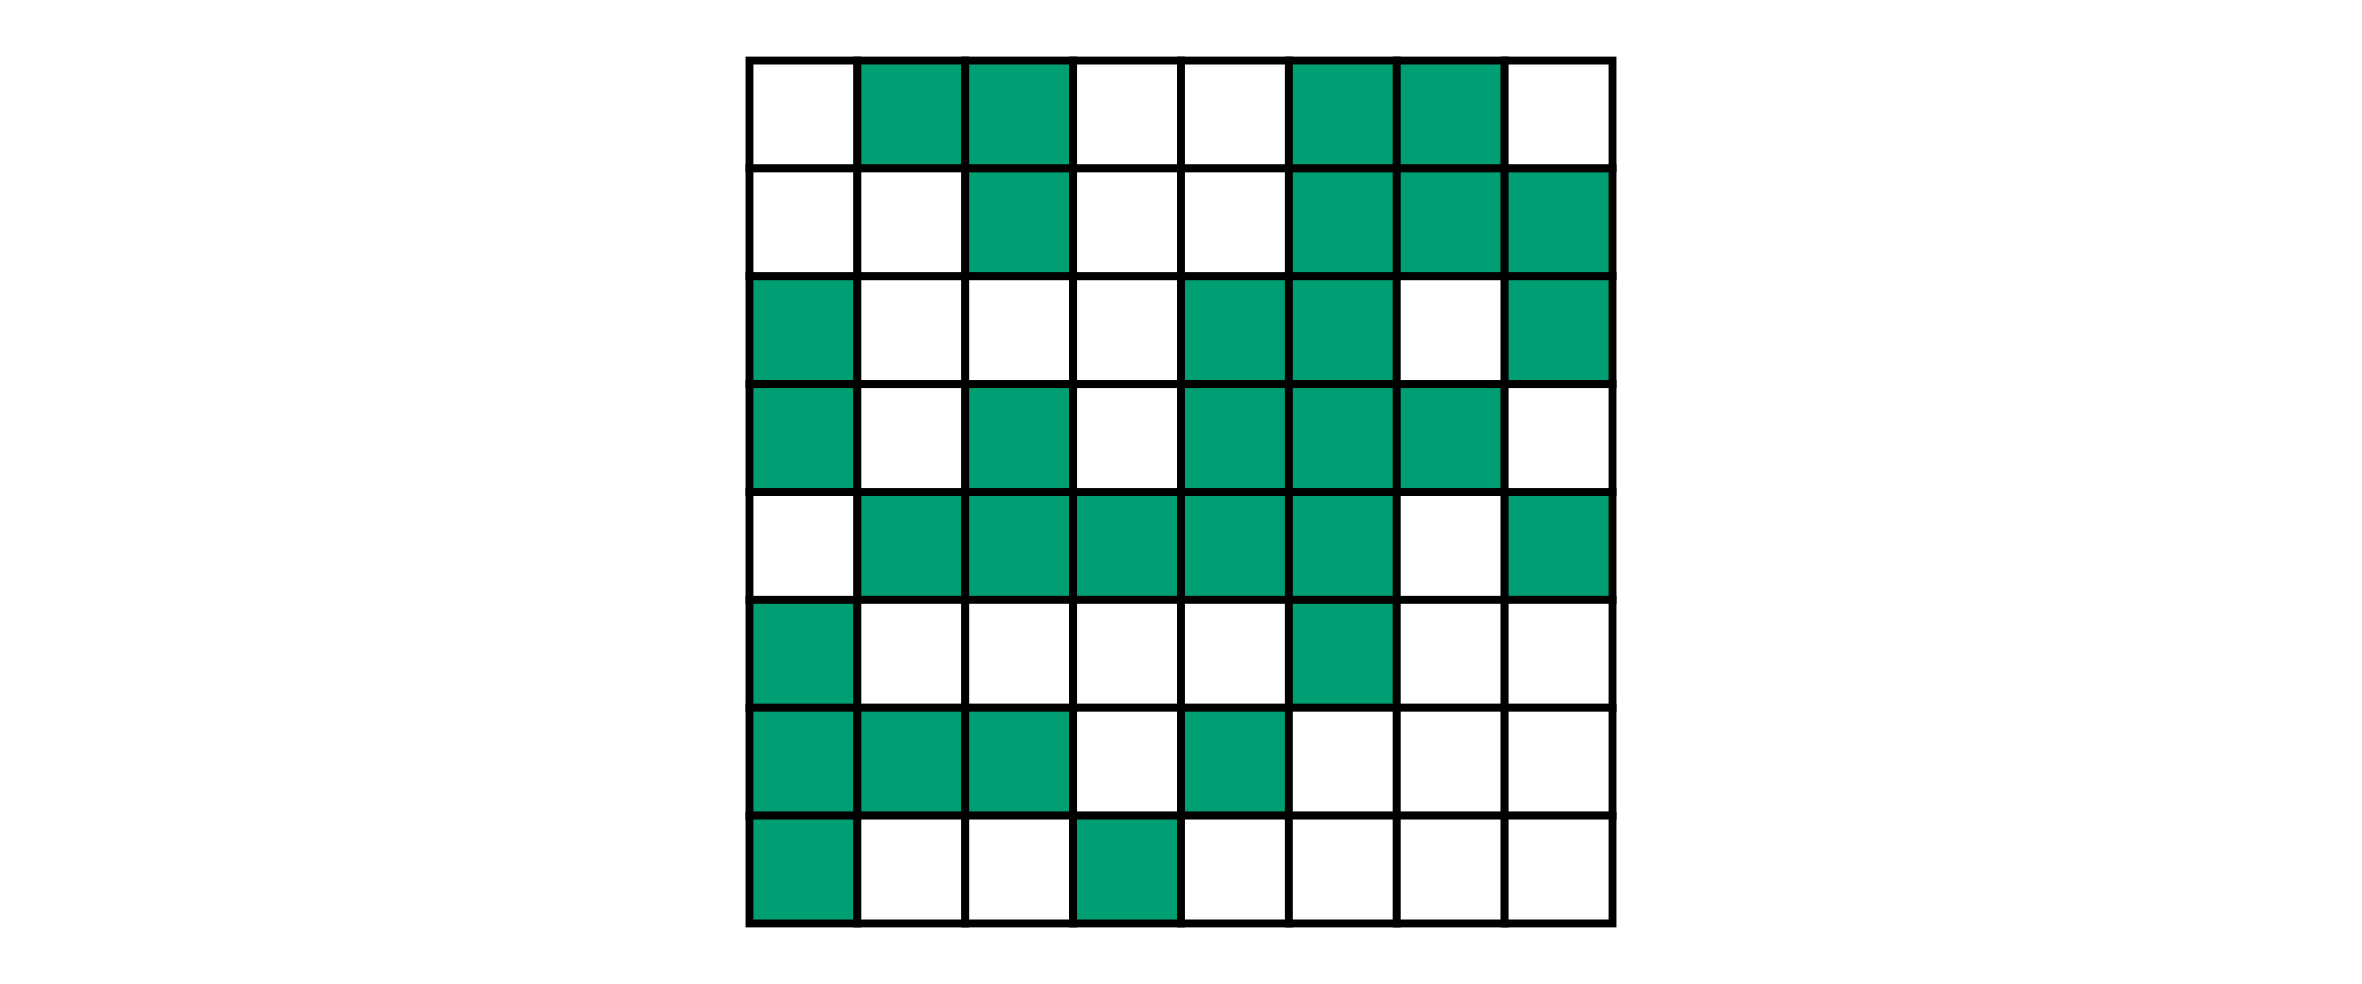
\includegraphics[width=\textwidth]{Figure 4.5.A}
\caption{Each cell independent in a Bernoulli random field}
\end{figure}
\noindent Such a random field is \textbf{spatiotemporally independent}\index{spatiotemporally independent} because each cell in this field of values does not carry any member of interaction across space $(i,j)$ or time $t$.
Specifically, the probability distribution for each cell is independent:
$$f(x_{i,j},t) \perp f(x_{i^*, j^*}, t^*)$$
for all $(i \neq i^*)$ OR $(j \neq j^*)$ OR $(t \neq t^*)$.

Random fields are at their most interesting when they are spatiotemporally dependent. Spatial dependence is useful for randomly generating terrain ins computer graphic, modeling, and video games. \textbf{Perlin noise}\index{Perlin noise} is used in the popular video game \textit{Minecraft} to randomly generate the height of a world's terrain:
\begin{figure}[H]
\centering
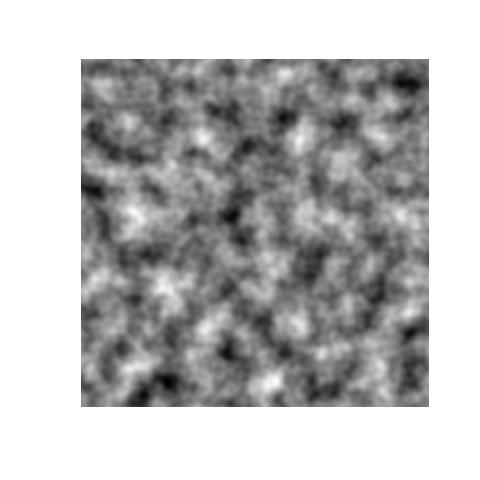
\includegraphics[width=\textwidth]{Figure 4.5.B}
\caption{Normalized Perlin noise $1000 \times 1000$}
\end{figure}
Perlin noise's spatial dependence is helpful because it does not require knowledge of the rest of the map to generate these spatial dependencies.

Would you consider a random walk or Brownian motion to be a random field? Perhaps not one particle, but many particles. Precisely what constitutes a random field is not nearly as formal and rigorous in its differentiation from the regular definition for a probability density function. All finite random fields may be represented using a finite Markov chain, though perhaps not always practical to simulate on a computer. All non-finite random fields may still have an infinite Markov chain representation such as an infinite simple random walk on $\mathbb Z^1$. An uncountably infinite random field would lack a Markov chain representation, even if its finite approximation on a computer does for reasons similar to the differentiable nowhere property of a Wiener process.

\section{Ising Model}
The \textbf{Ising model}\index{Ising model} is a stochastic process representing the magnetic moments of magnetically-interacting particles arranged as a rectangular lattice. A $d$-dimensional Ising model with dimension lengths $(n_1,...,n_d)$ has $\prod n_i = N$ total cells or spin sites, and each site $x$ on the lattice $X$ may take values $x \in \{ -1, +1\}$ representing its \textit{spin}.
\begin{figure}[H]
\centering
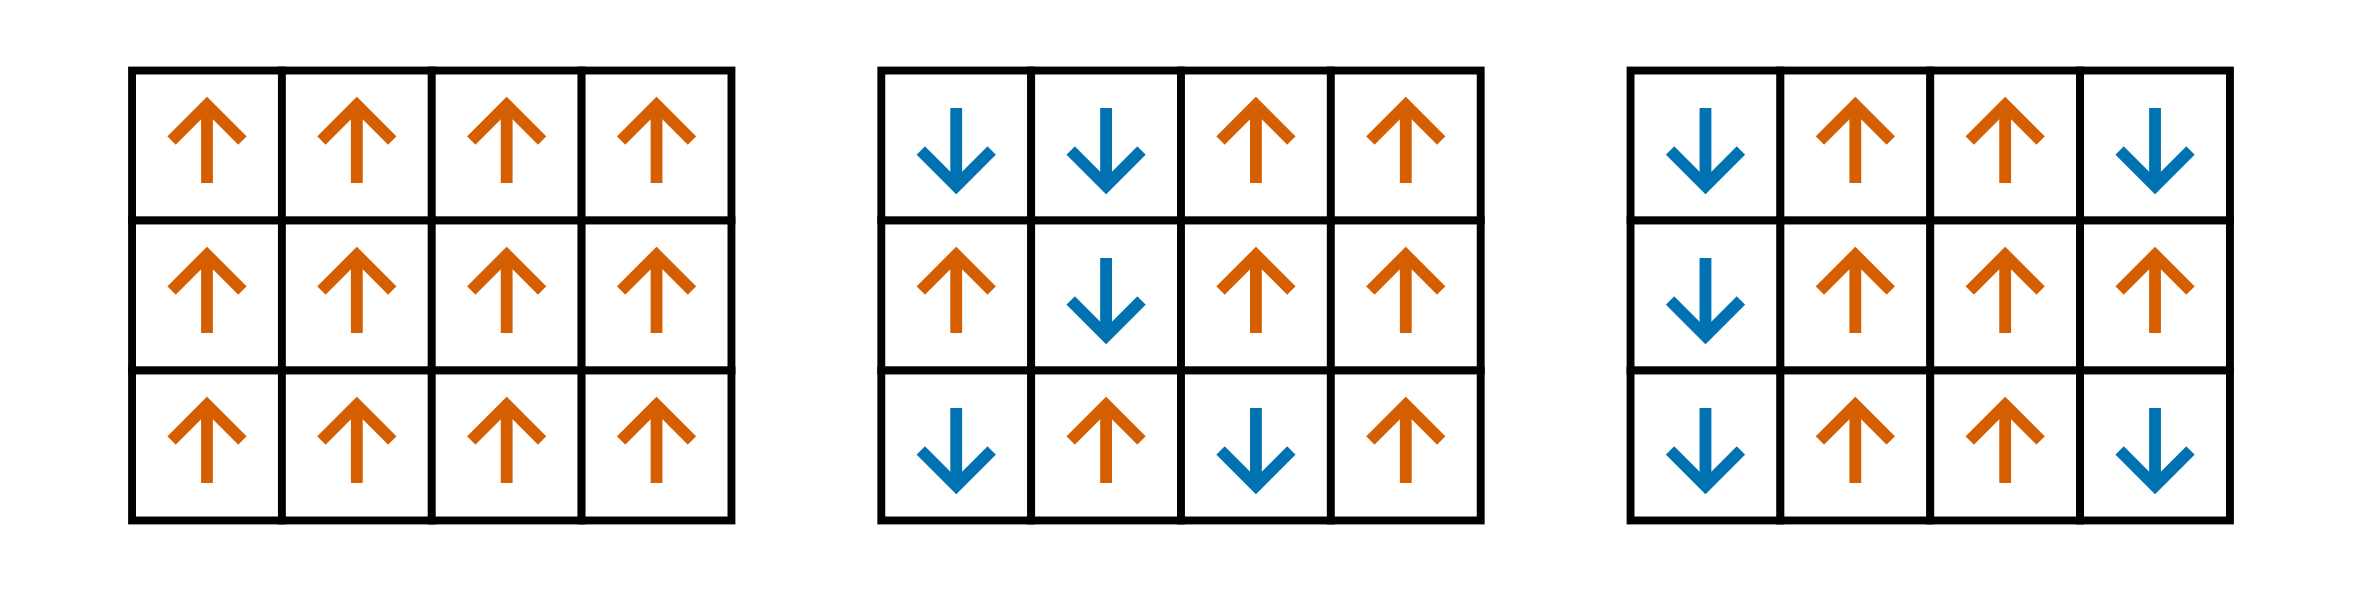
\includegraphics[width=\textwidth]{Figure 4.6.A}
\end{figure}
\noindent At low temperatures, the spin of sites tend to align. At high temperatures, the spin of sites flip randomly and independently similar to a Bernoulli random field.

Between low and high temperatures lies the \textbf{critical temperature}\index{critical temperature} in which the information flowing in a site equals the information flowing out. Rather, internal entropy of a site equals the external entropy of a site. Instead of external determinism or internal randomness purely, their influences are balanced such that information of a cell propagates radially:
\begin{figure}[H]
\centering
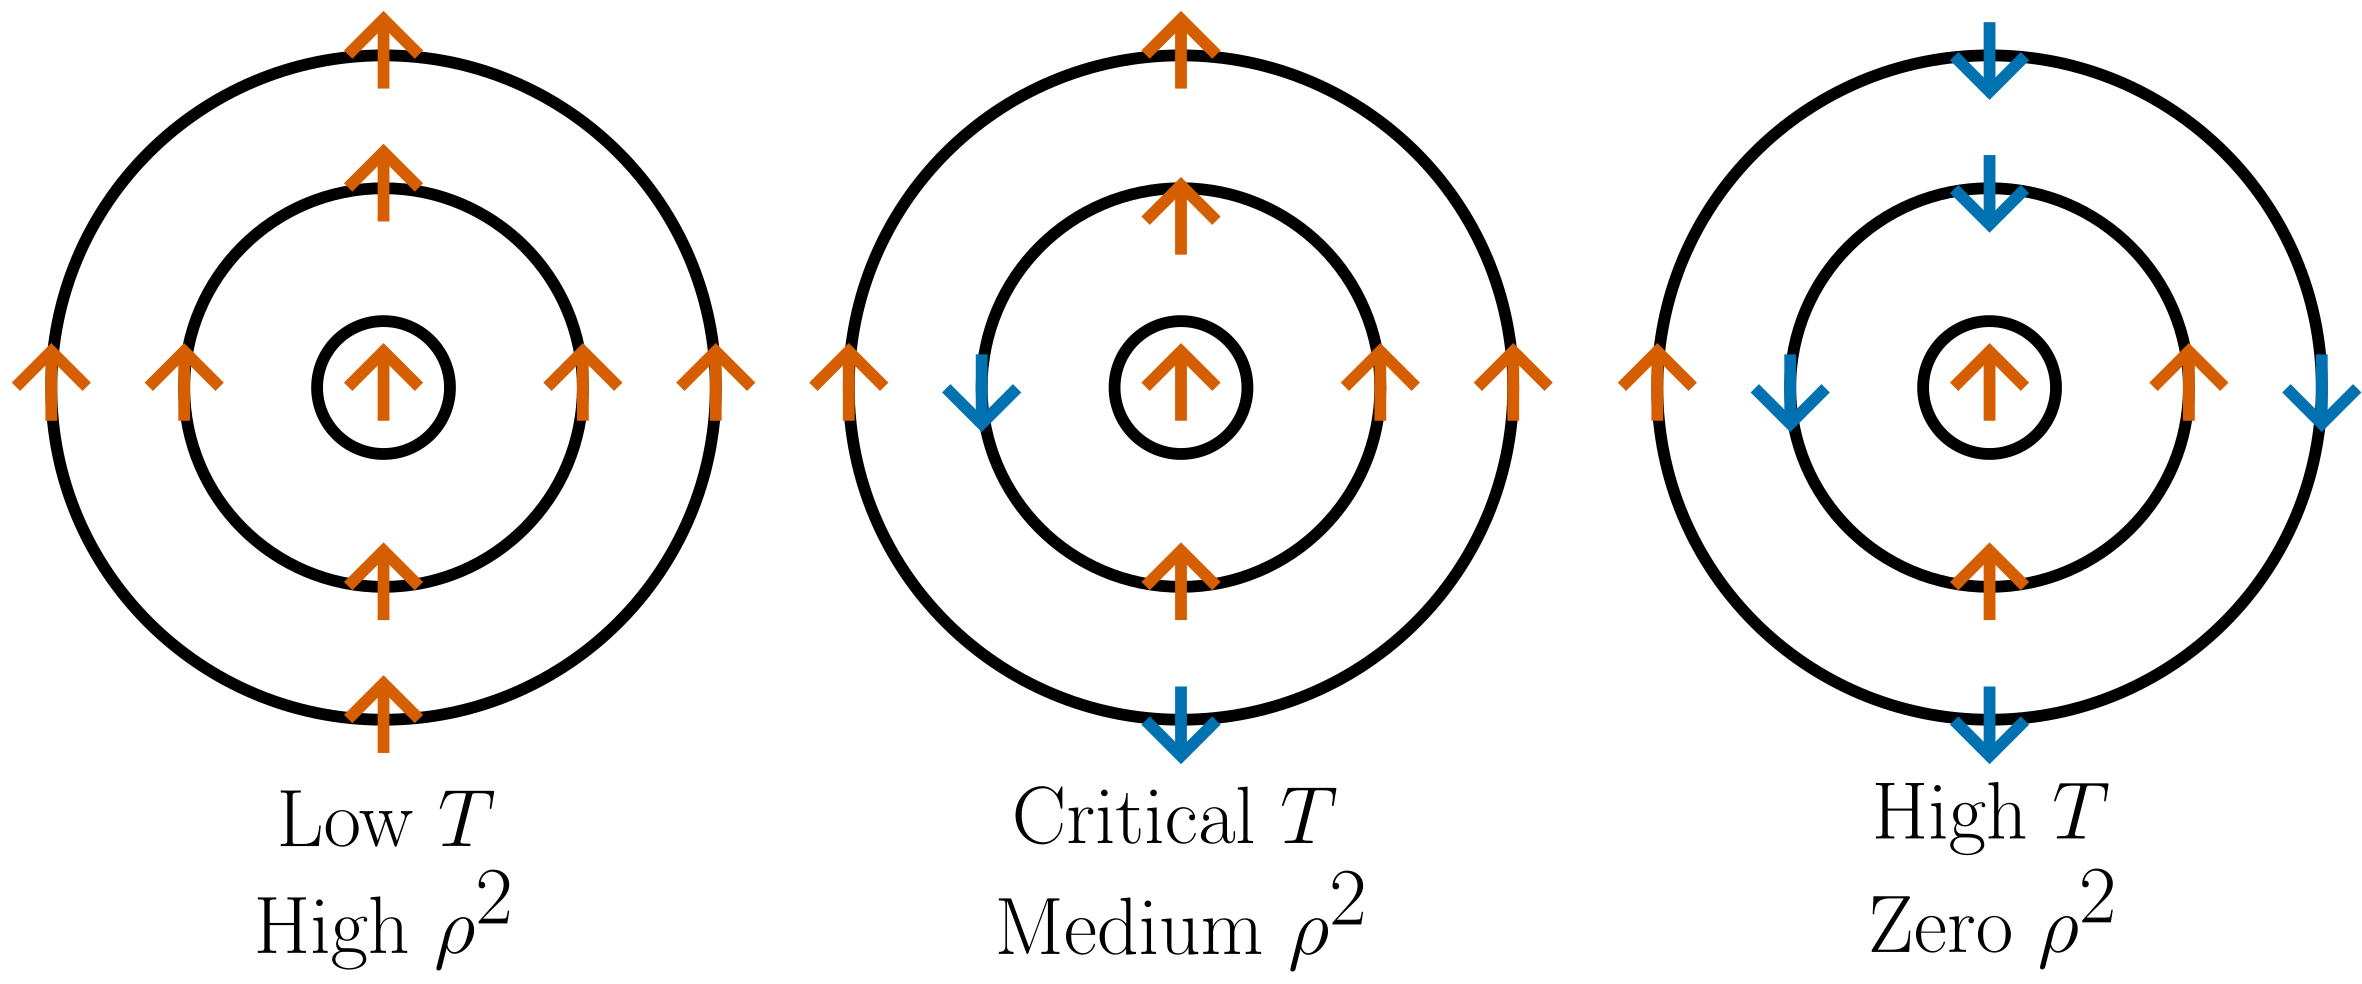
\includegraphics[width=\textwidth]{Figure 4.6.B}
\caption{Low temperature systems $T$ have high spatial correlation $\rho^2$}
\end{figure}

Each ring represents the \textbf{information horizon}\index{information horizon} in space for different time scales. At a small radius for distance, adjacent influence is immediate. At a long radius for distance, influences takes time and is itself influenced as it gets there. The information density of each ring depends on the dimensionality and temperature of the lattice $X$. With an analytic solution to the Ising model, it is possible to express the stochastic influence between two sites exactly. There is currently no analytic solution to the 3D Ising model, if it even exists. There is an analytic solution for the $2$-dimensional case found by Onsager for a non-magnetic field.

The $3$-dimensional case may not be exactly solvable, due to the fact that it is an \textbf{NP}-complete problem as discussed in \textit{\S 6.8 Computational Complexity}. We consider the Ising model as a type of \textit{\S 5 Cellular Automata}.


\chapter{Cellular Automata}
\section{Motivations for Learning Cellular Automata}
A \textbf{cellular automaton}\index{cellular automaton} is a discrete-time, discrete-space system whose cell values or cell classes change over time. Each cell in the space interacts with its neighborhood of cells during each time step depending on the definition of neighbor. The von Neumann neighborhood is the classic definition that involves orthogonal neighbors while the Moore neighborhood includes orthogonal and diagonal neighbors:
\begin{figure}[H]
\centering
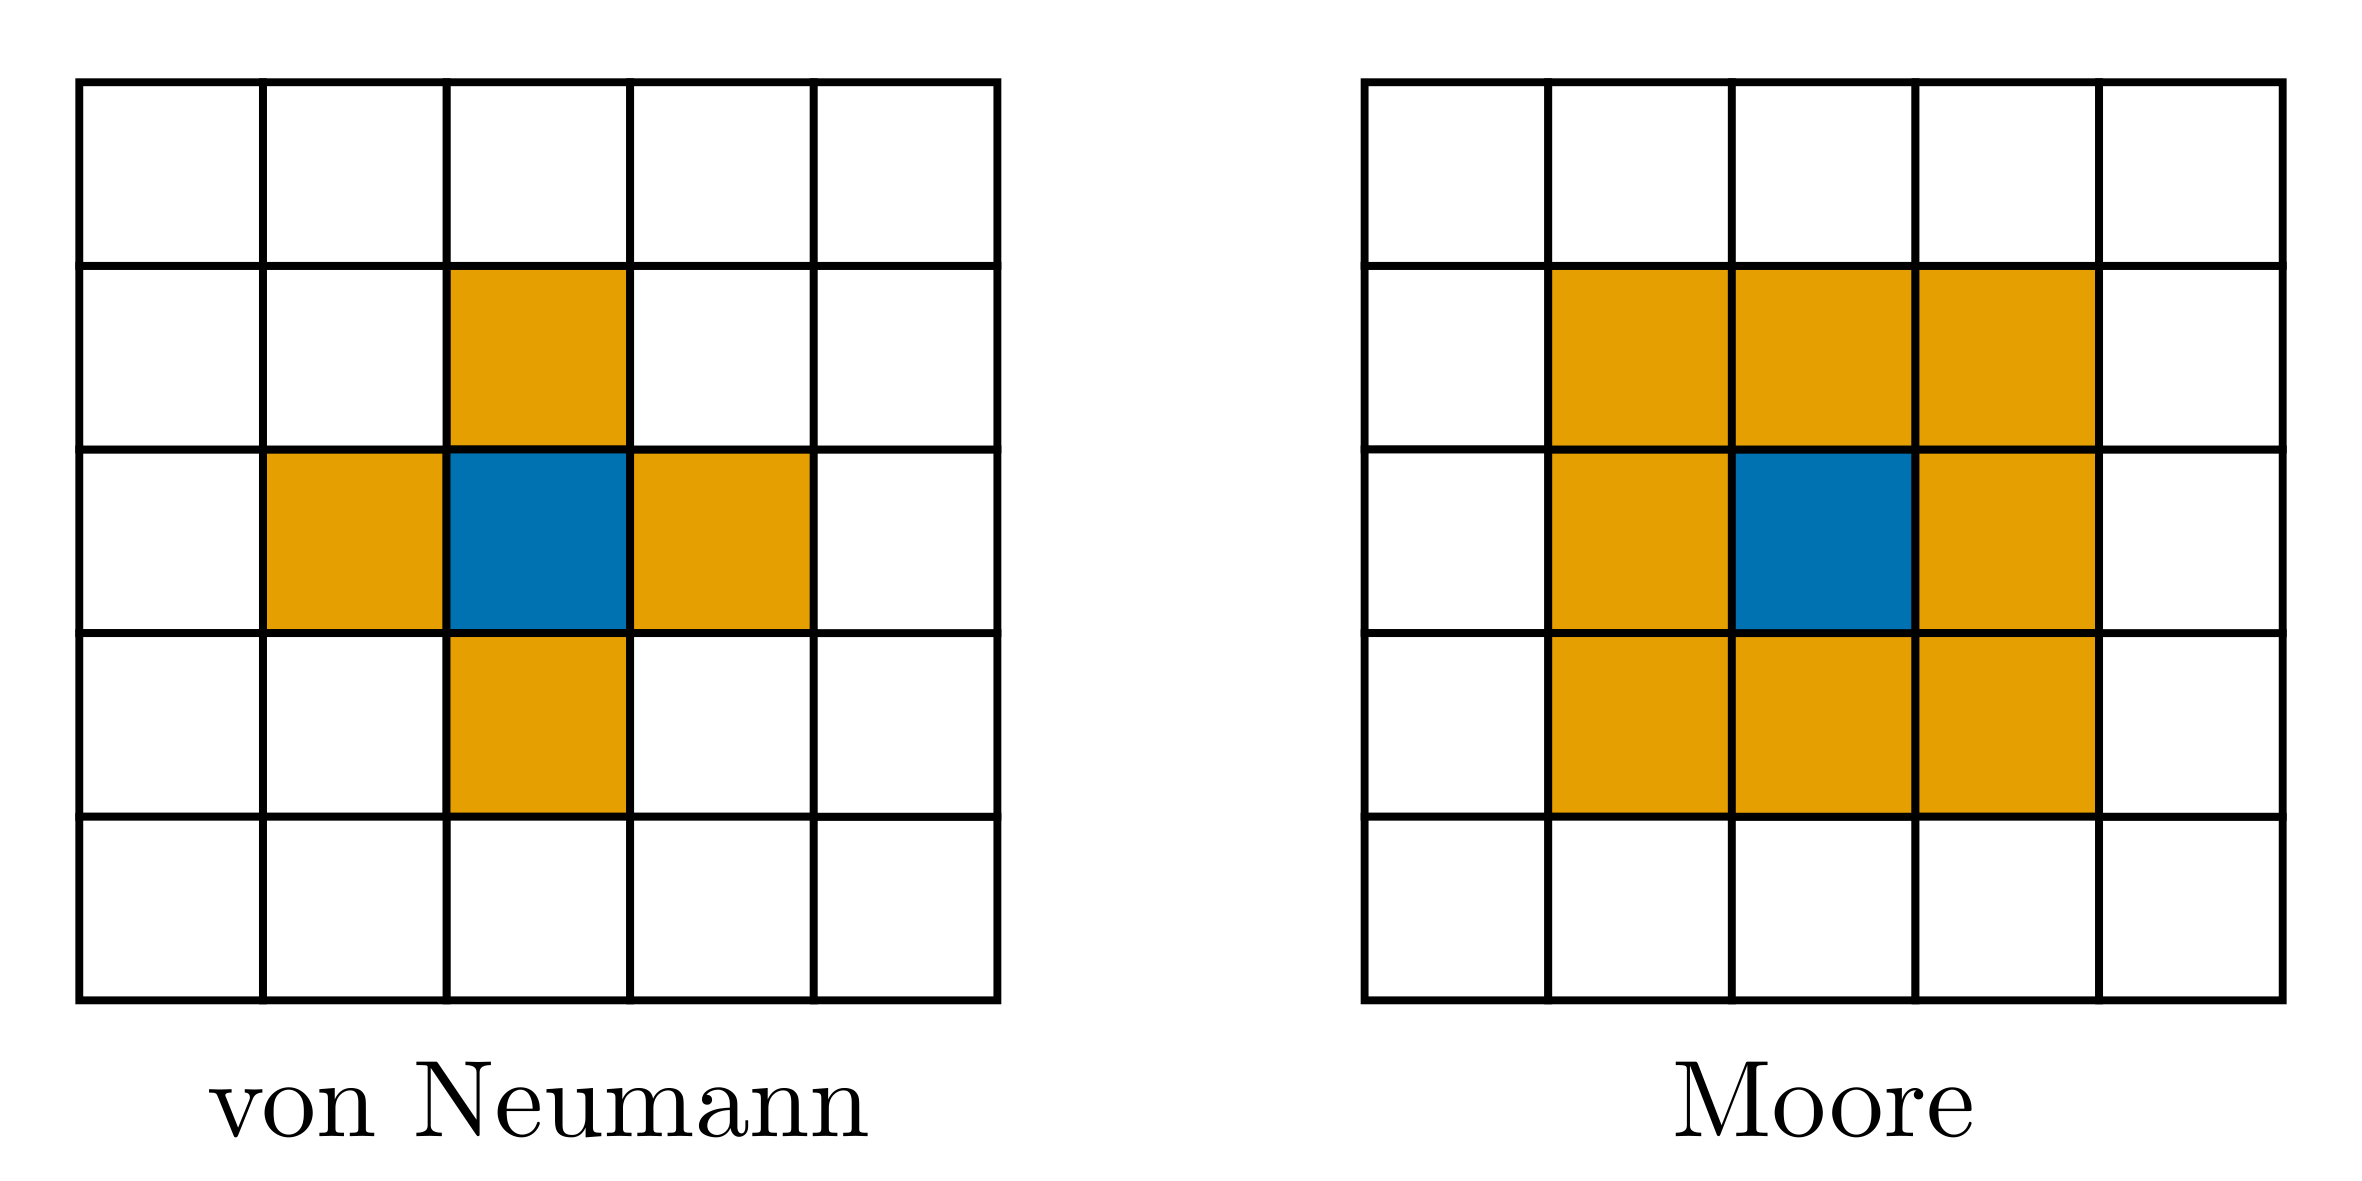
\includegraphics[width=\textwidth]{Figure 5.1.A}
\caption{The von Neumann and Moore neighborhood}
\end{figure}
\noindent 
These adjacencies are alternatively called the first-order neighbors and the second-order neighbors respectively. Using this information, the system $X_t$ updates to $X_{t+1}$ according to the transfer operator $\Lambda$. Cellular automata typically occur on grids or square lattices such as graph paper. Each cell $x$ must be an element of some common set such as $x \in \{-1, +1\}$ or $x \in \{0,1,2,...\}$.

Boolean random walks have an important question: is our proposed solution the \textit{unique} solution to generalizing random walks? There may be other possible transition functions or transfer operators to consider that are \textbf{bisimulations}\index{bisimulation} of the simple random walk. Specifically, simple random walks must be produced as a subset of the transfer operator $\Lambda$.

At the time of writing, there is no known binary cellular automata that have the properties of stochastic, synchronous, dichromatically symmetric, unbiased, and non-degenerate. Consider the following stochastic cellular automaton in which each cell's future state probability depends on the proportion of von Neumann neighbors:
\begin{figure}[H]
\centering
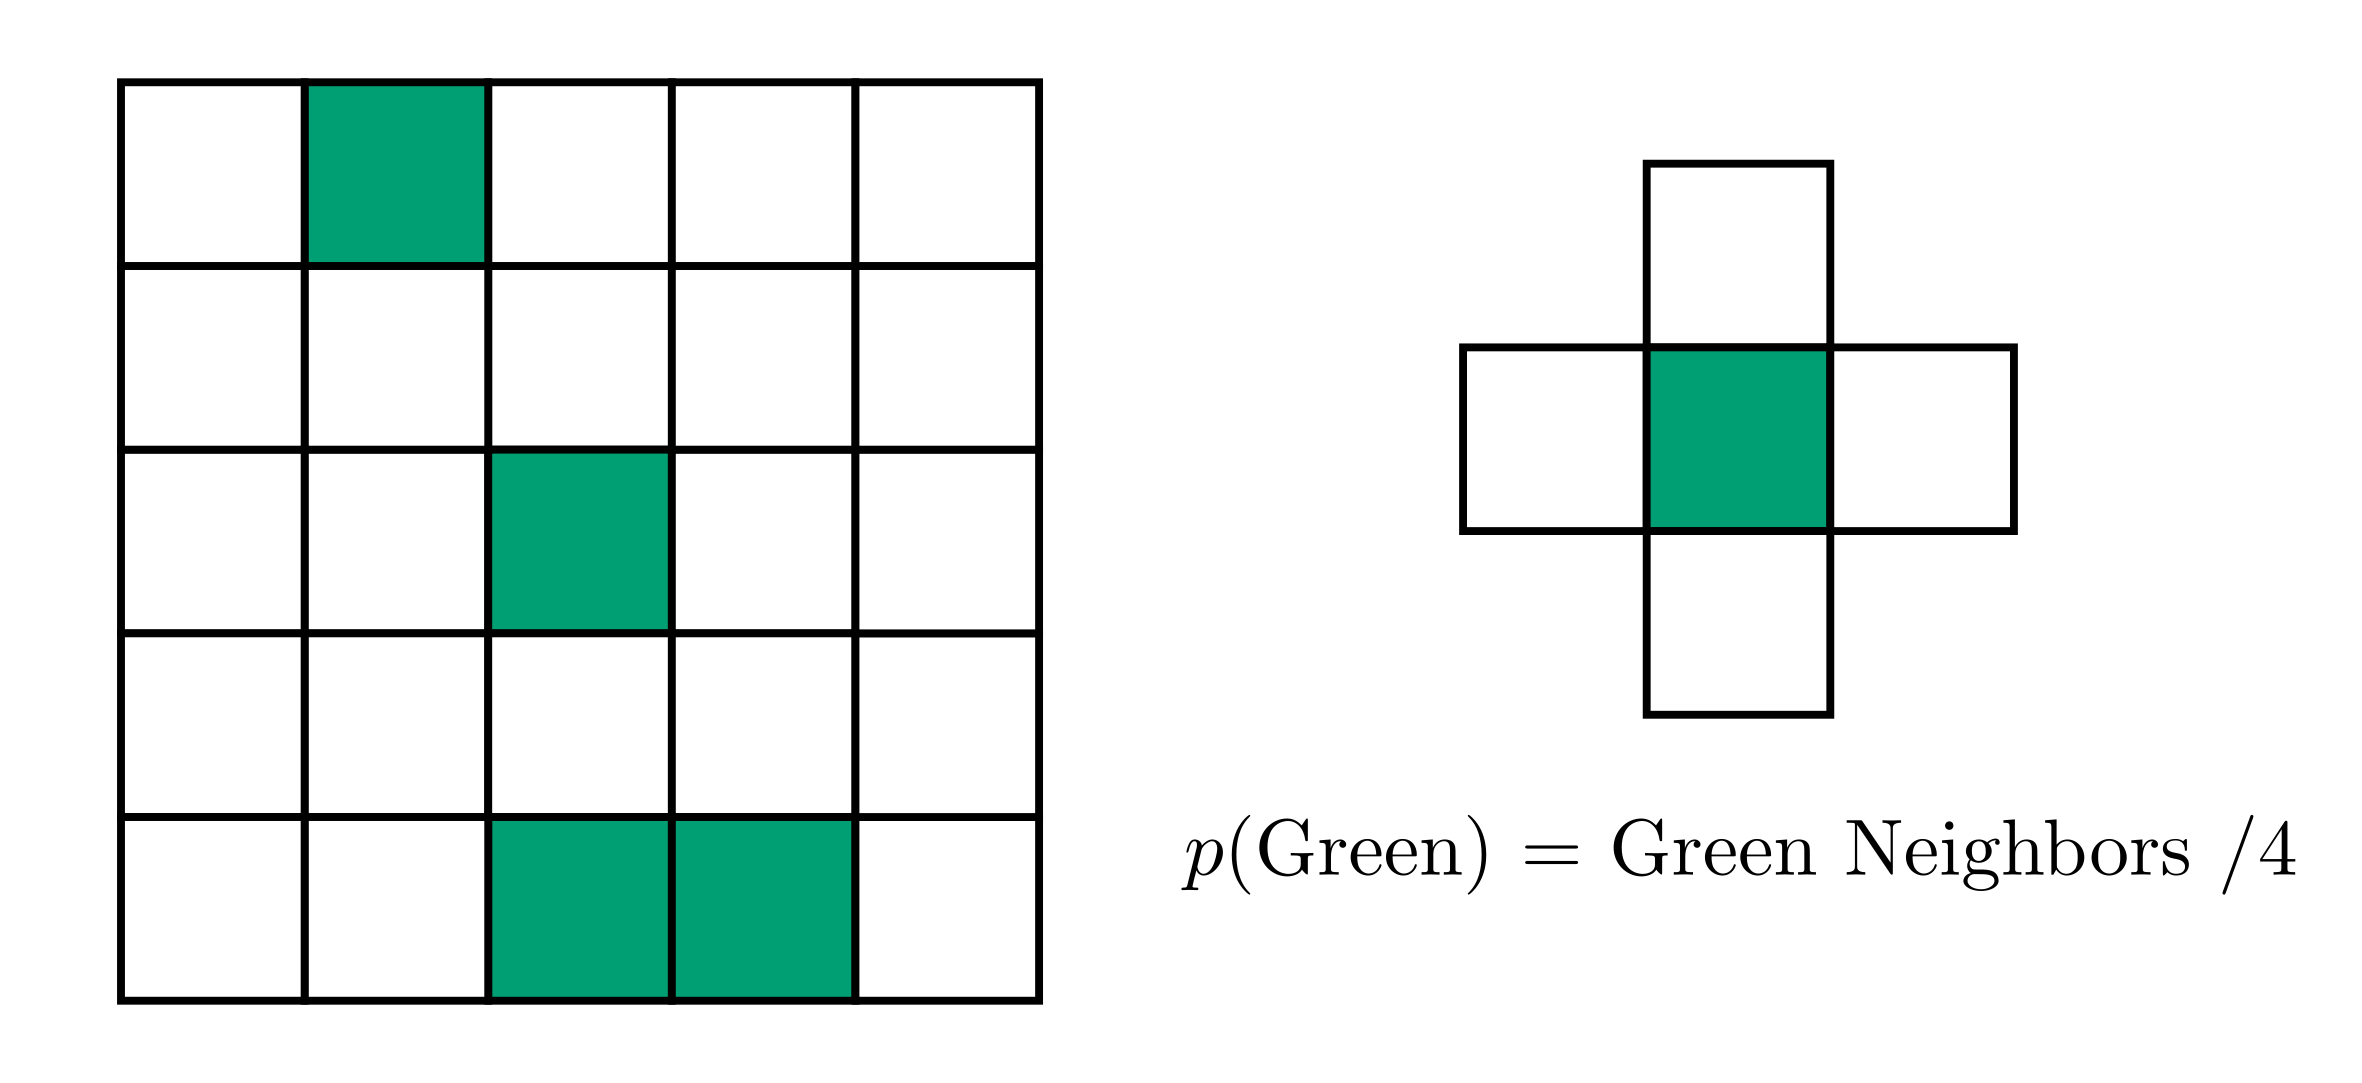
\includegraphics[width=\textwidth]{Figure 5.1.B}
\caption{A simple random cellular automata's probability depends on neighbors only}
\end{figure}
\noindent Due to depending strictly upon neighbors, all configurations must eventually degenerate to all $x = -1$ or all $x = +1$, a state in which it will never recover. Ideally, every state in the state space $\mathcal X$ is recurrent and ergodic, and each cellular transition only depends on its immediate while simultaneously being dichromatically symmetric. A Boolean random walk depends on a maximal independent set, which means parallel computation is not possible in a single time step.

Why should we care about cellular automata at all? Cellular automata define simple models with emergent complexity, sometimes enough to represent all computable functions. Physical models as we know it depend on the world around us being computable, thus something that may be simulated or measured with a computer. \textbf{Digital physics}\index{digital physics} is the speculative idea that the universe as we know it can be represented as the output of a probabilistic computer.

Will your model of the world change if you think of viruses at attempting to unravel your code? If you think of chemical processes as an encryption-decryption process, or the stars as only being capable of moving in motions computable? What does it mean if the Standard Model of particle physics must behave according to the properties of computable functions? What does it mean that we measure these particles with computing devices? Is matter merely encrypted light?

\section{Conway's Game of Life}
John Horton Conway developed a cellular automaton known as the \textit{Game of Life} in 1970. The system for \textit{Life} evolves according to the following transition rule on a 2D grid with two classes available for each grid cell: live or dead. The state of a cell at the next time step depends on the following rules:
\begin{enumerate}
\item Any live cell with fewer than two live von Neumann neighbors is a dead cell after one time step.
\item Any live cell with two or three live von Neumann neighbors is still a live cell after one time step.
\item Any live cell with more than three live von Neumann neighbors is a dead cell after one time step.
\item Any dead cell with exactly three live von Neumann neighbors is a live cell after one time step.
\end{enumerate}
This transition function is deterministic and thus depends strictly on the initial state $X_0$ after one time step. A state with no possible prior state except itself is called a \textit{garden-of-Eden} state, and therefore is only possible as an initial state $X_0$. For \textit{Life}, every state $X$ in the state space $\mathcal X$ has a unique state that it may transition to. However, some states may have multiple possible prior states that it may have transitioned from.

The following are examples of \textit{still life} patterns that stay the same over successive generations:
\begin{figure}[H]
\centering
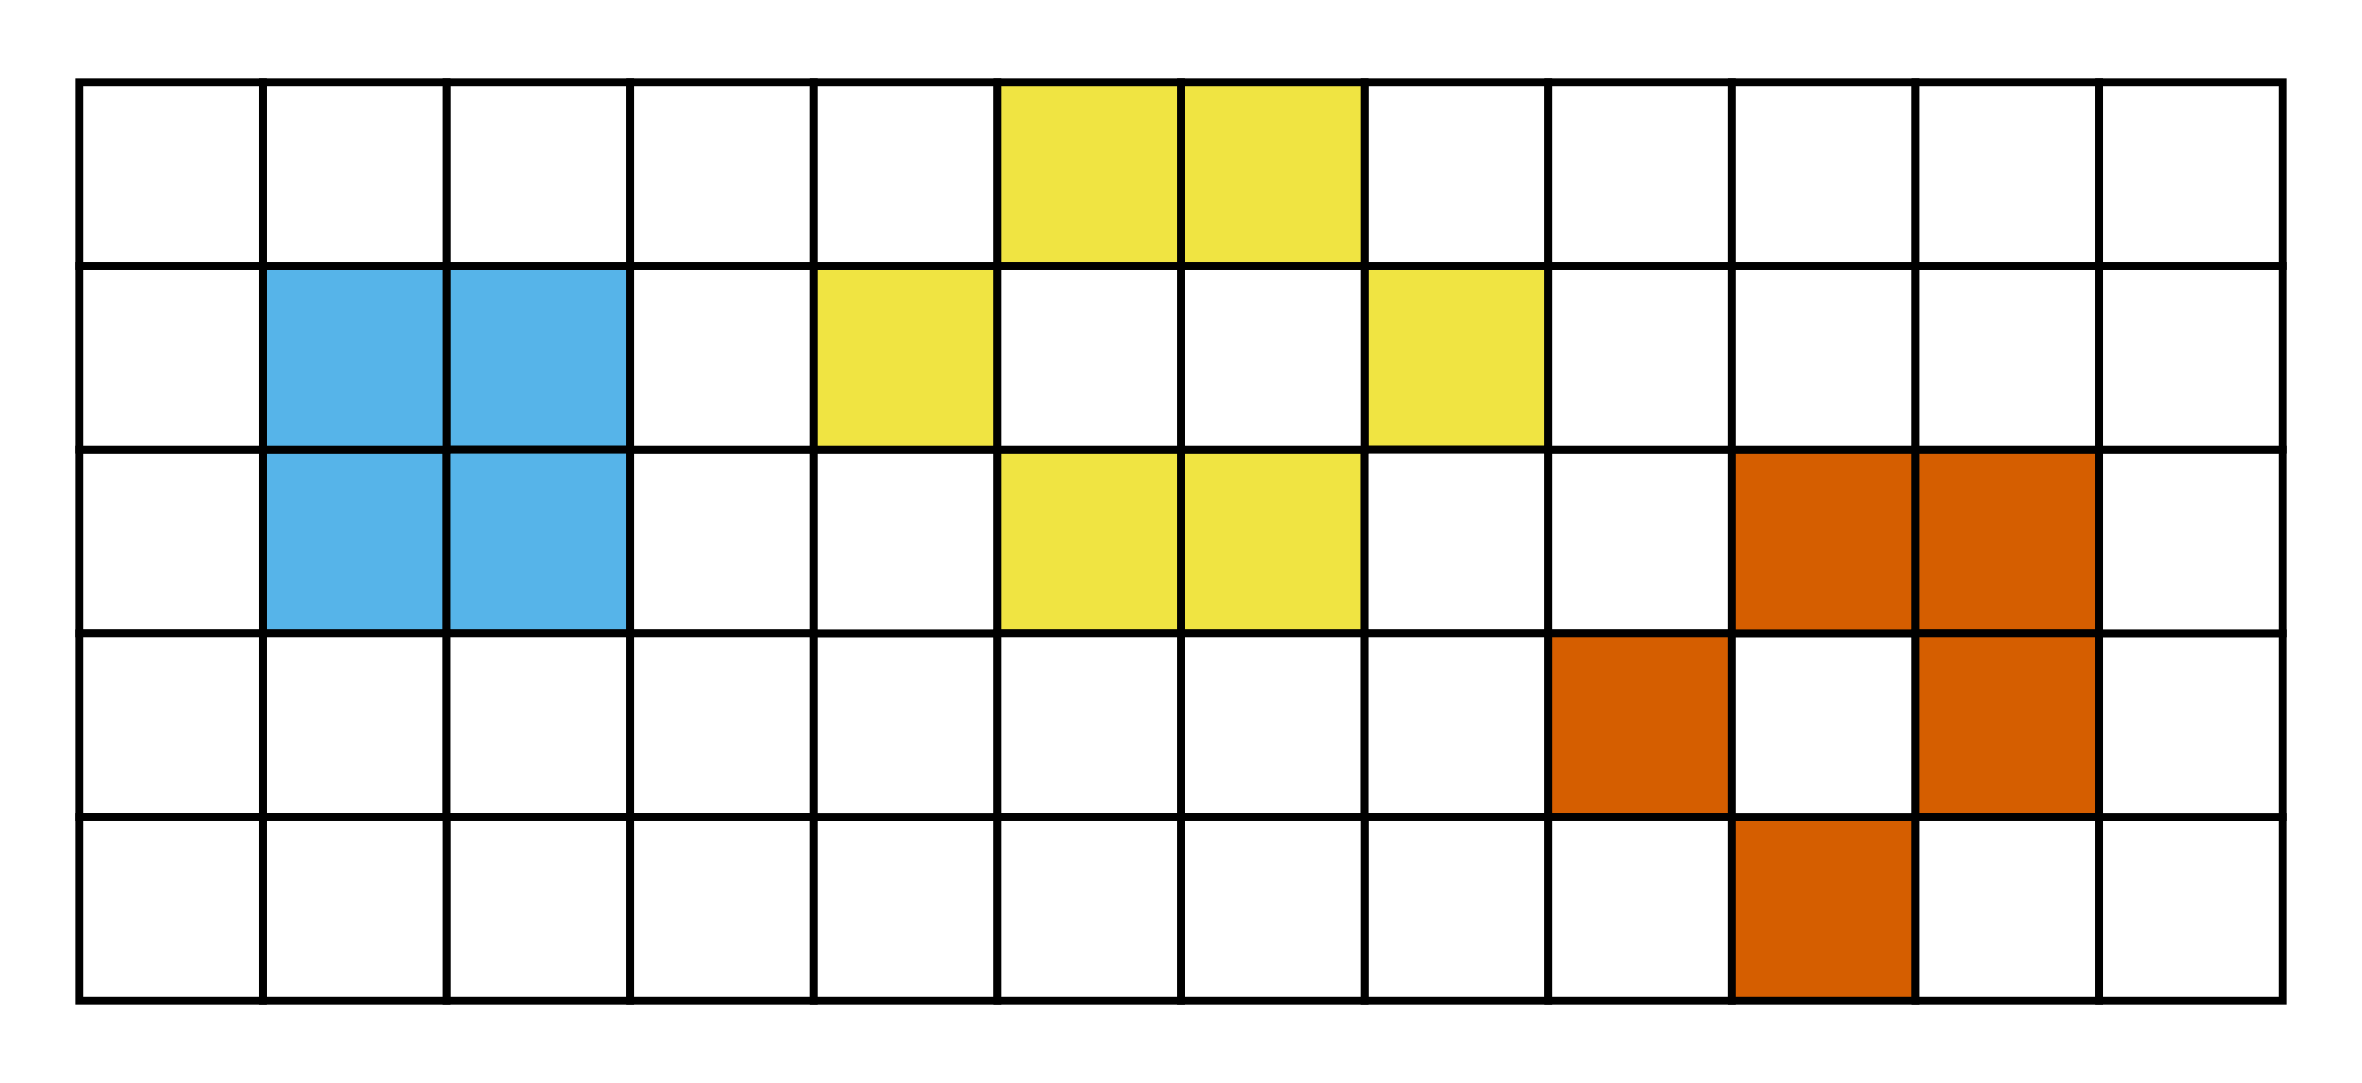
\includegraphics[width=\textwidth]{Figure 5.2.A}
\caption{Common still lifes: a block, a hive, and a boat}
\end{figure}
\noindent
These patterns or subsystems are called aperiodic or $1$-periodic due to completing a cycle of states after a time period of $1$. A pattern with a period of $2$ or more is called an \textit{oscillator}. Still life patterns tend to survive under random initial states $X_0$ until interacted with, and this interaction is a ``measurement'' by some ``external'' computing device. In technicality, it is incorrect to claim that there is a difference between a measurement device within the system and the system itself.

In Conway's \textit{Life}, it is possible to simulate any universal \textbf{Turing machine}\index{Turing machine} since the transition function of the cellular automaton is \textbf{Turing complete}\index{Turing complete}. We can create a finite computer that stores memory and evaluates memory through the construction of logic gates such as AND, OR, and NOT gates. A larger construction of cells, macrocells, can act as a form of memory storage. A moving pattern called a \textit{glider} can interact with a macrocell to measure its representation from the Boolean set $\mathbb B_\pm = \{-1, +1\}$. A relatively simple memory cell can be implemented using the aforementioned still life patterns and gliders:
\begin{figure}[H]
\centering
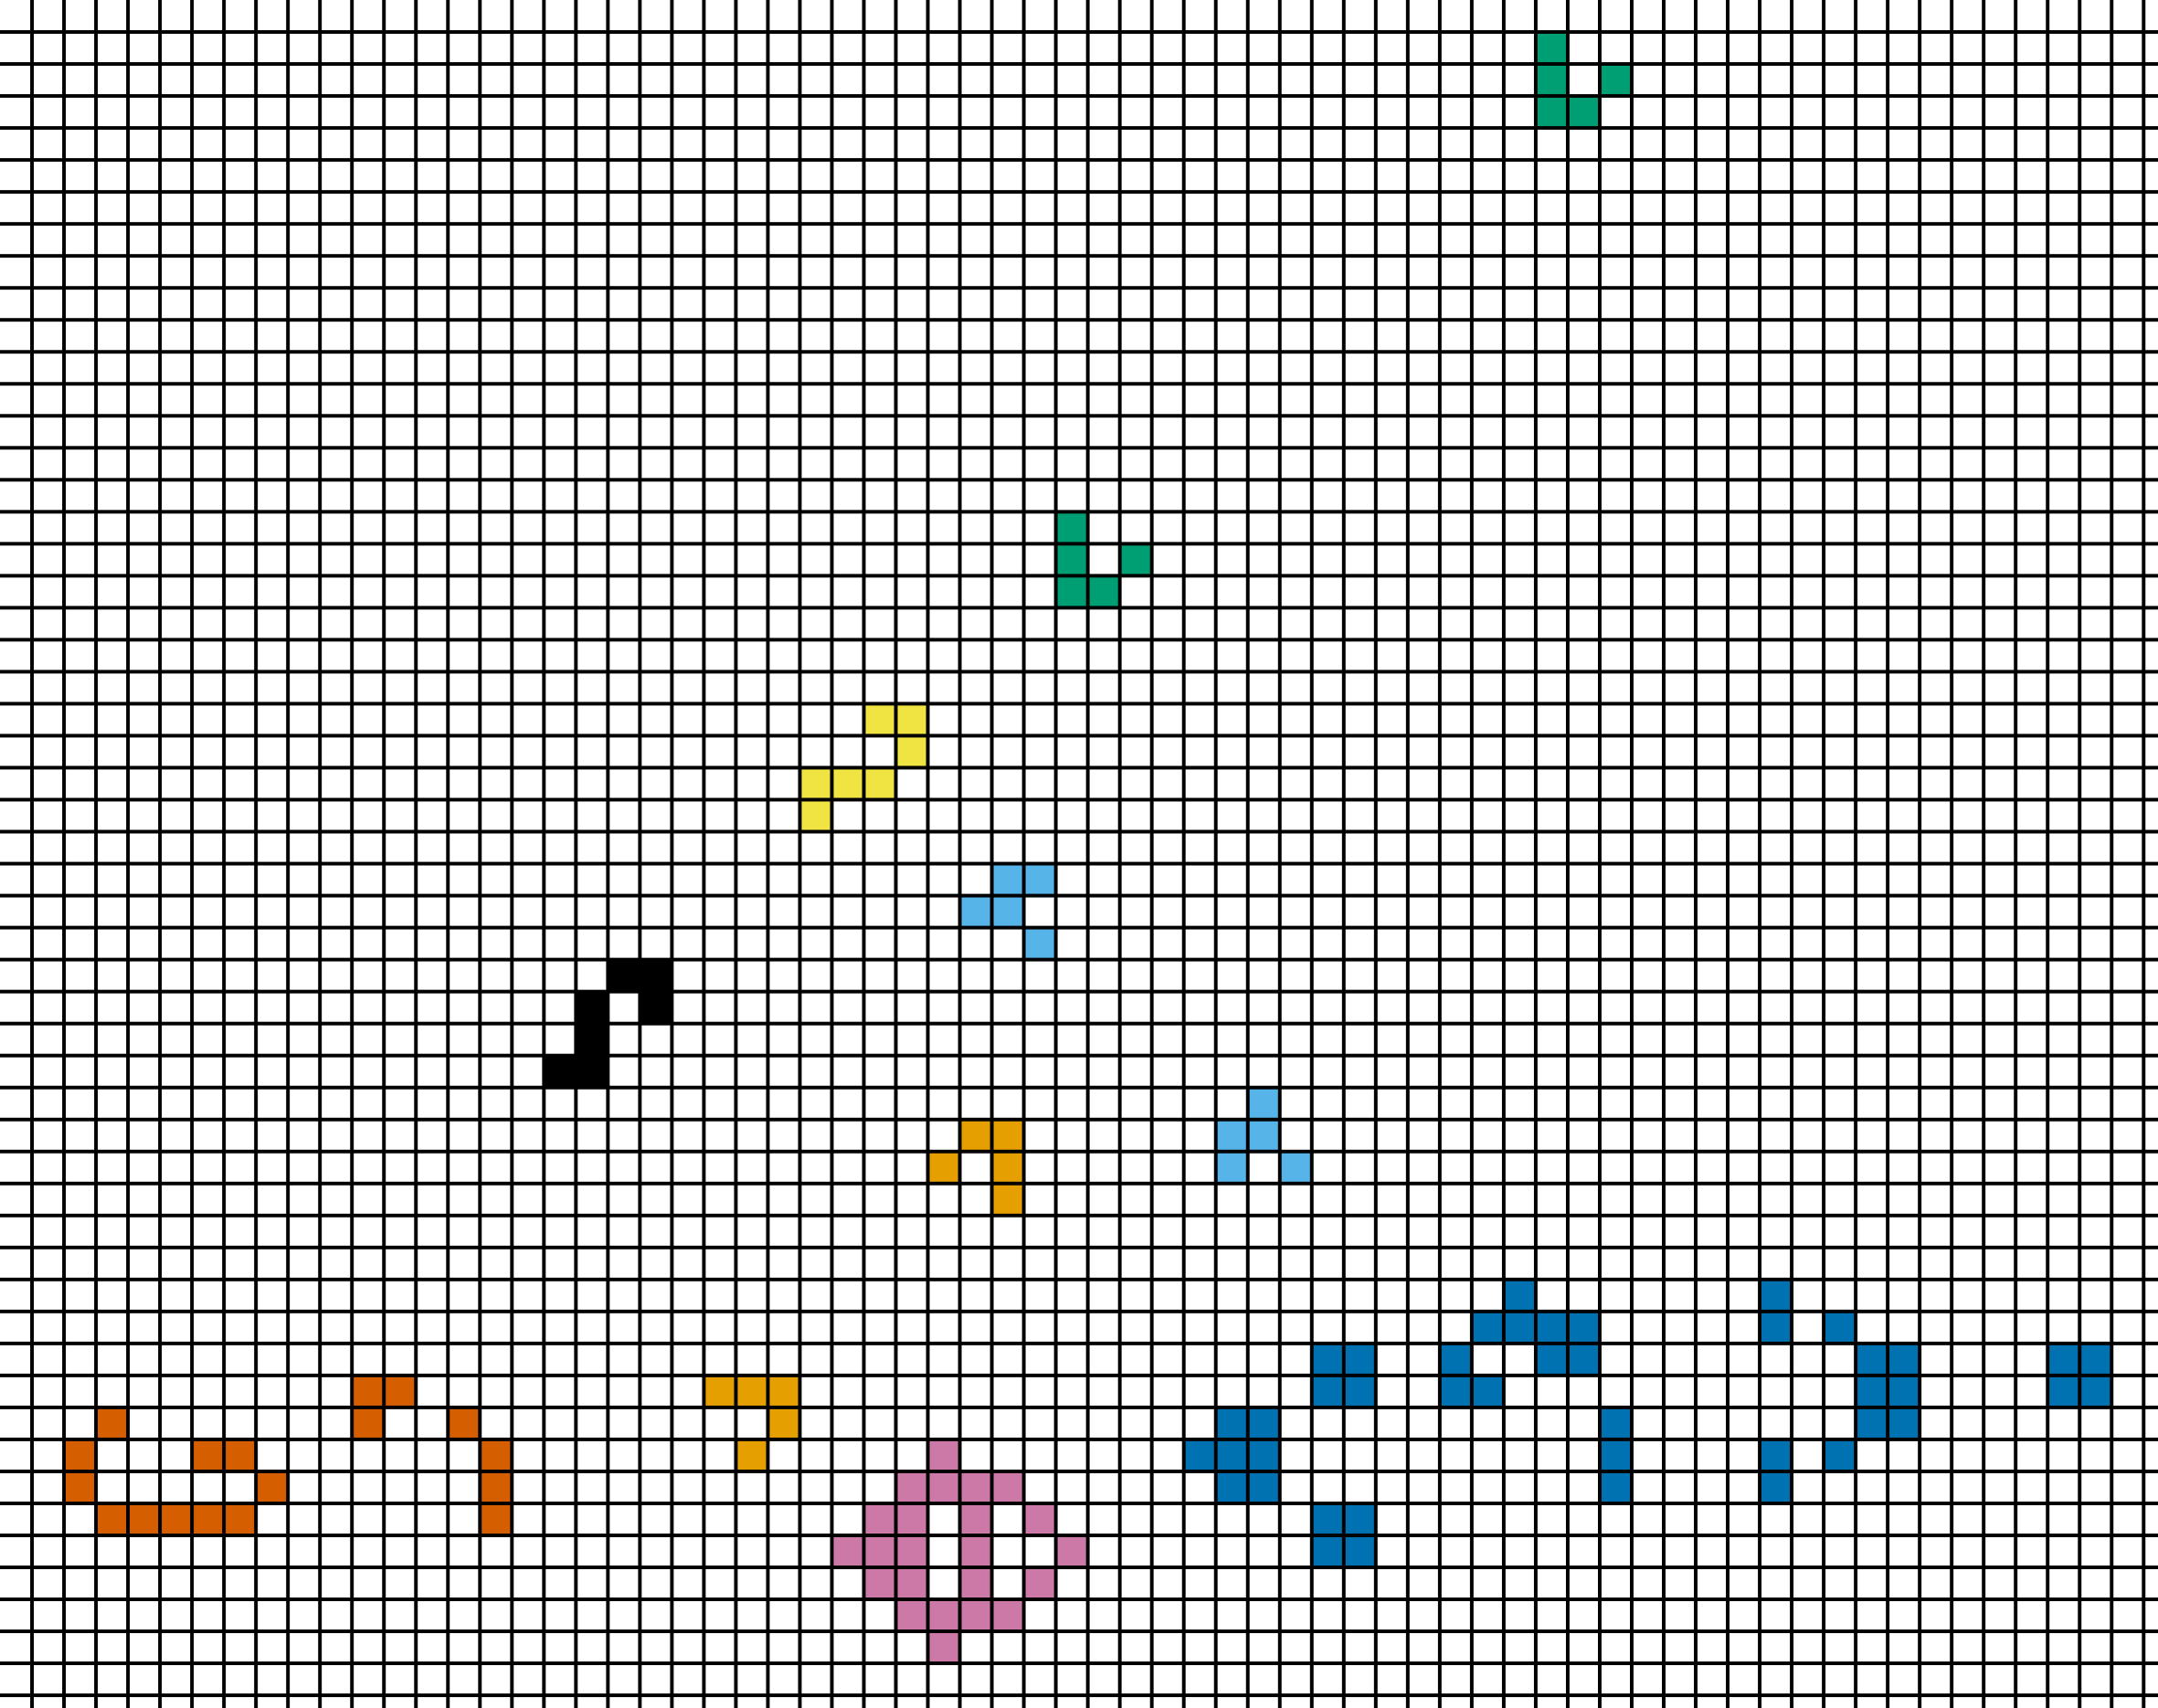
\includegraphics[width=\textwidth]{Figure 5.2.B}
\caption{NOT logic gate: input green gliders stop output blue gliders}
\end{figure}
\noindent This pattern returns a glider of the memory cell represents $+1$ and returns nothing of the memory cell represents $-1$. We can perform more complex tasks if we use \textit{glider guns} that infinitely produce gliders, \textit{eaters} which delete gliders, and \textit{reflectors} which reflect gliders. If a finite structure in \textit{Life} can generate and negate glider streams, then we have the properties necessary to create logic gates and thus finite computers.

The use of more complex macrosystems allows us to create larger and more general computers. All measurements constitute an interaction between systems. We shall define \textbf{measurement} as an interaction that preserves some measure $\mu(\cdot)$ according to the rules of set theory. Conway's \textit{Life} quickly kills off any sort of computational structure that is not measure-preserving for some implied metric. Unstable patterns or representations may represent many possible things such as logical contradictions or divergent computations such as infinities. 

Any emergent system that fails to be measure-preserving in some sense erases itself so quickly so as to be imperceptible. It is by definition and construction that the only stable systems are measure-preserving, whether than measure is bits, energy, or some other implied object in \textit{Life}. For an object to be perceivable and predictable, it is important that objects are in non-probability measure $\mu$ if and only if they are similar in probability measure $p$.

Why is it important to consider whether or not Conway's Life is or is not a measure-preserving dynamical system in some abstract, unidentifiable, or implicit space? The temporal reversal of Conway's \textit{Life} has degenerate states called \textit{garden-of-Eden} states from which it may never recover. The random selection from a set of viable time reversed states will inevitably return itself to one of these Eden states. The equivalent for time advancement for continuous functions is known as degeneracy, but for flavor we may wish to call them \textit{Last Judgment} states in this case. A digital physics model of the universe must have no Edens and no Judgments, else the universe fails to exist.

\section{Properties of Cellular Automata}
Cellular automata may be classified according to key properties about their transition function $f$. Conway's Life is the most well-known 2D cellular automaton, and its transition function is deterministic and synchronous. It is the prototypical example of a cellular automaton, and these properties and more assumed to be true by default for most cellular automata. Many diverse and complex cellular automata may emerge when we break these rules.

A cellular automaton is said to be \textit{deterministic} if for a \textbf{transition function}\index{transition function} $f(\cdot)$ and given state at time $t$ if its forward time transition is precisely one state with probability $1$ under probability measure $\mu$:
$$\mu( X_{t+1} = f(X_t)) = 1$$
for all possible states $X_t$. A cellular automaton is said to be \textit{stochastic} under the transition function $f(\cdot)$ if there exists a probability measure such that any future has a probability less than $1$:
$$\mu( X_{t+1} = f(X_t)) < 1$$
for some initial state $X_0$. We can alternatively assume that all cellular automata are stochastic by default unless the entropy of a transition is precisely zero:
$$S(X) = -\sum\limits_{X \in \mathcal X} \mu(X) \ln(\mu(X)) = 0$$
for all possible transitions from every initial state. Therefore, a cellular automata is deterministic if and only if the entropy of a transition function $f(\cdot)$ of all configurations $X$ in the state space $\mathcal X$ is $0$.\footnote{A Markov chain is deterministic if and only if the entropy rate from every initial state is zero.}

A cellular automaton is said to be \textit{temporally synchronous} if the transition function $f(\cdot)$ updates all cells in $X_t$ to $X_{t+1}$ simultaneously, or if the update order of individual cells is unimportant. The key characteristic is that the transition function is statistically independent to update order via the Markov property. Synchronous updates via preprocessed data does not count.\footnote{There must exist an algorithm to update the entire system state with $O(1)$ time complexity.}

A cellular automaton is said to be \textit{spatially local} if the transition function $f(\cdot)$ of each cell in $X_{t+1}$ only depended on itself and its neighbors in $X_t$ via the Markov property. The key characteristic is that the transition function is statistically independent of non-neighbors per time step. 

A cellular automaton that fails both of these properties is \textit{spatiotemporally non-local}, and it is possible to have all-to-all dependency between cells in the system. A non-local transition function means that a cell is statistically dependent upon non-neighbor cells, and this may require information on possible orderings of the transition or some sort of mutual exclusion.

The humble $2 \times 2$ oscillator in Conway's \textit{Life} is synchronous and local. It depends only on its immediate neighbors, and nothing about its update rule provides statistical information about update order:
\begin{figure}[H]
\centering
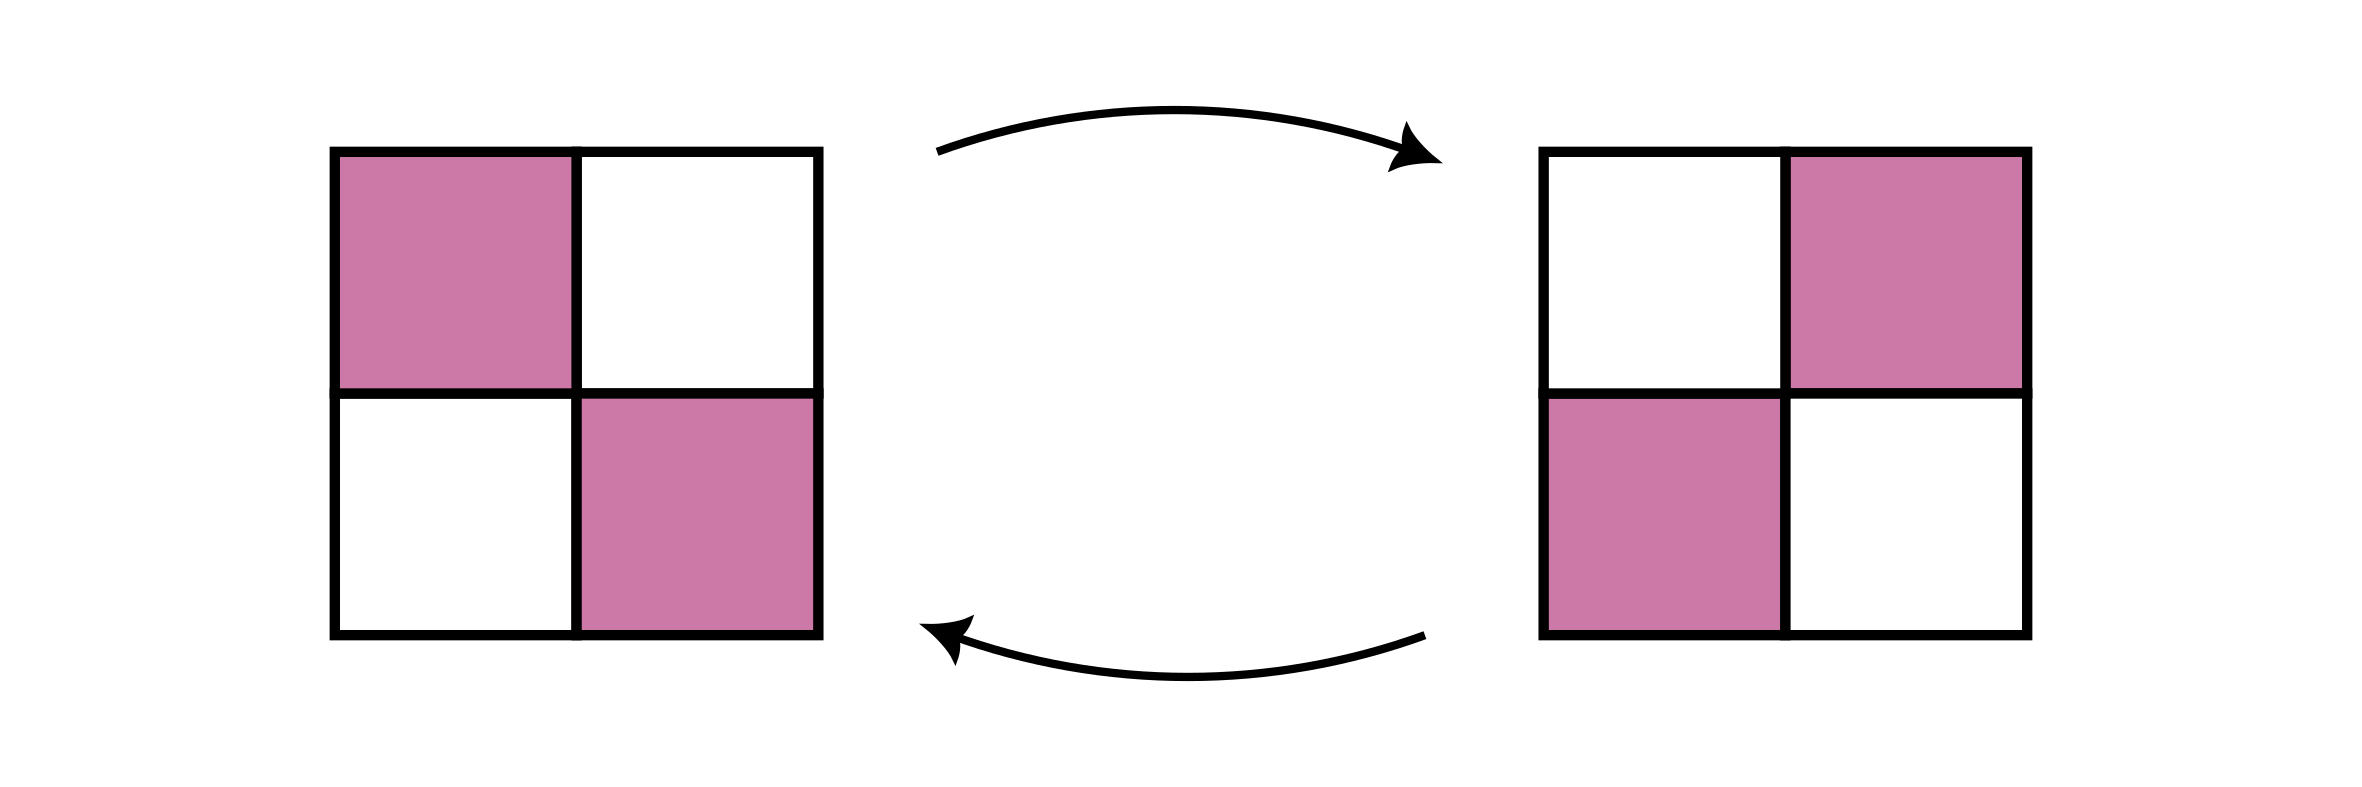
\includegraphics[width=\textwidth]{Figure 5.3.A}
\caption{\textit{Life} $2 \times 2$ oscillator}
\end{figure}
\noindent
However, Boolean random walks is strongly non-local. This is because particles cannot occupy the same space, therefore the outcome of each transition depends on the resolution of other cells. In a checker pattern, one cell's resolution depends on the next cell's probability, influencing the next cell's probability, influencing the next cell's probability, and so on in an irreducible cascade:
\begin{figure}[H]
\centering
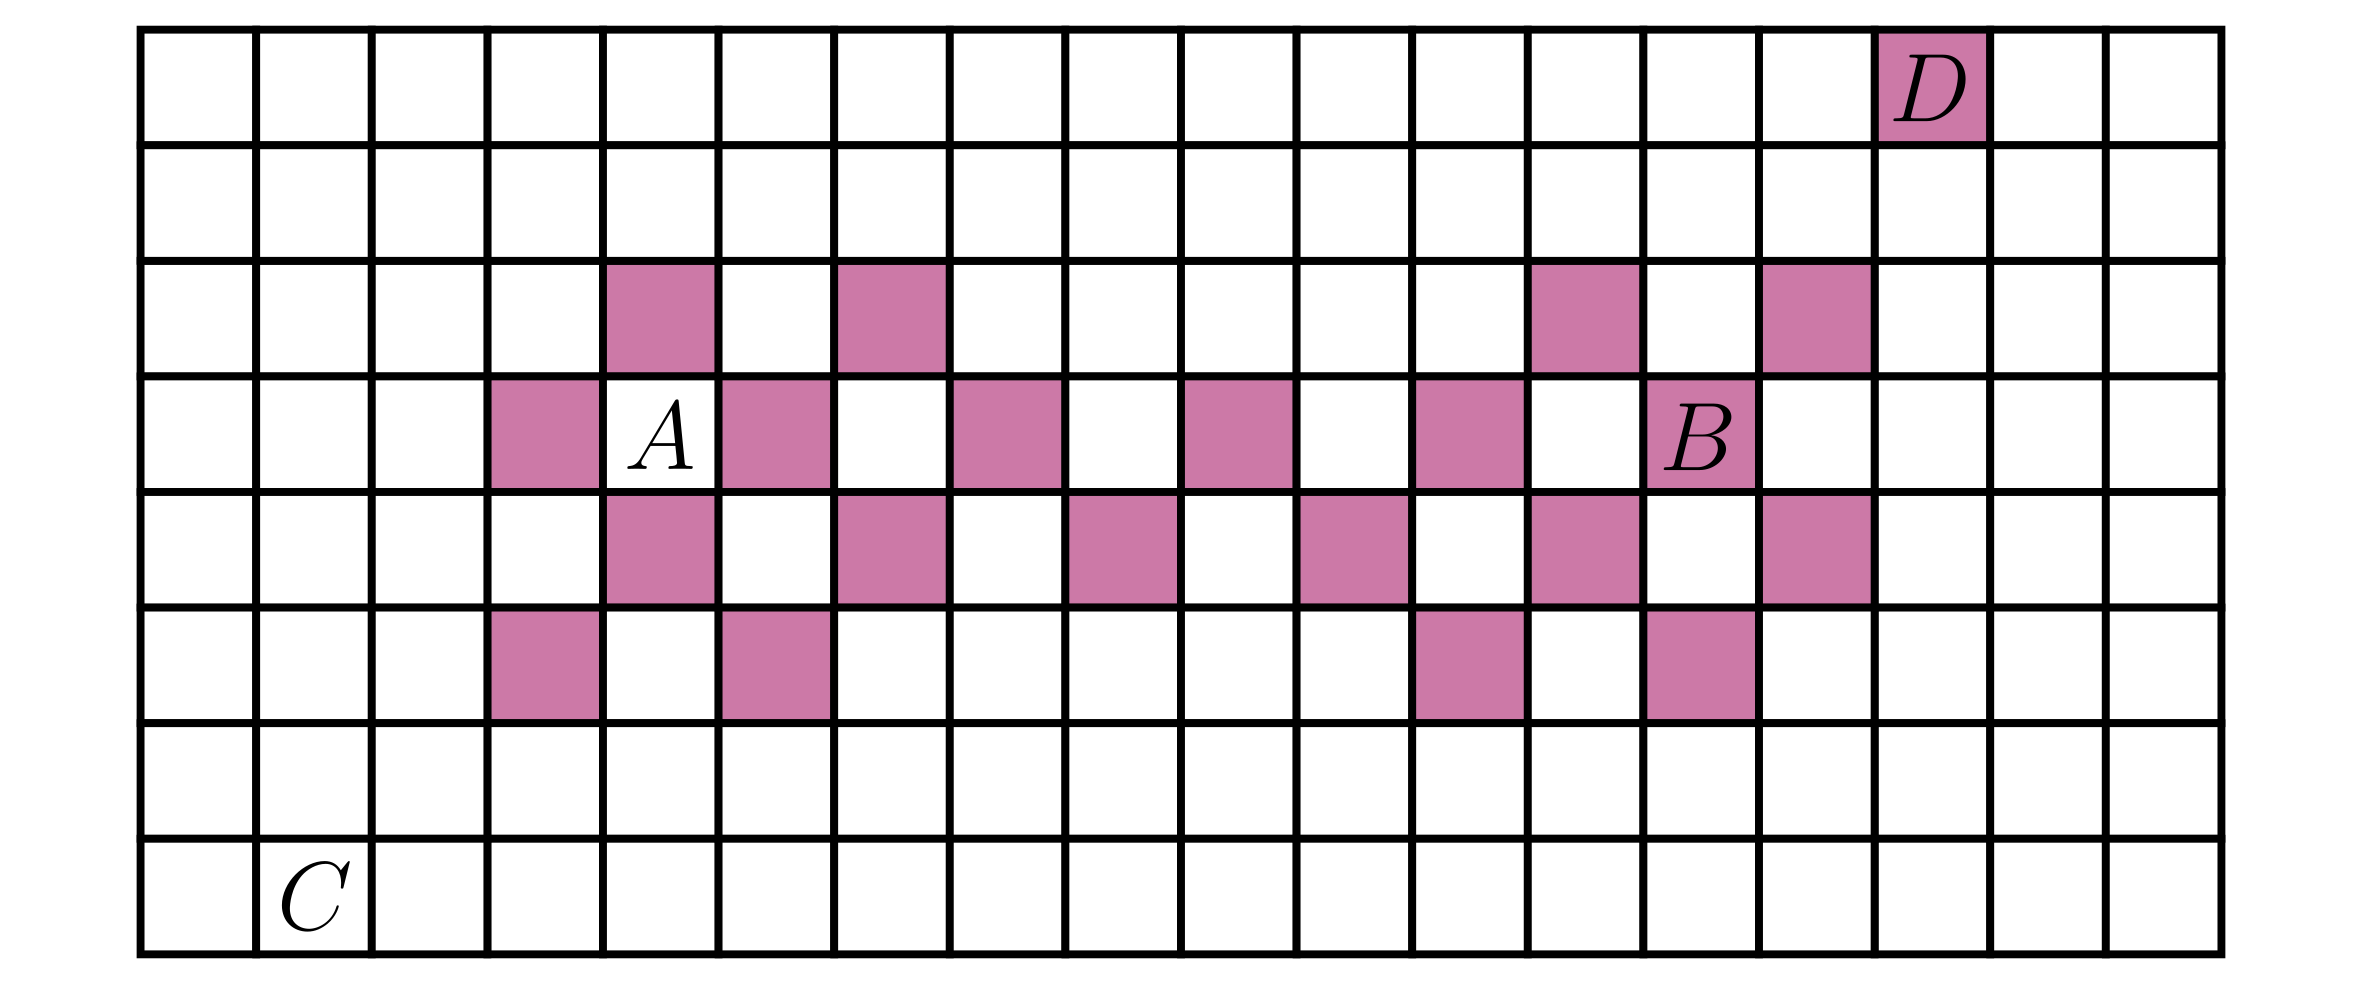
\includegraphics[width=\textwidth]{Figure 5.3.B}
\caption{Boolean random walks non-local dependency of $A$ to $B$ due to checkering. The next step future of $C$ is independent of $D$ due to a lack of checkering.}
\end{figure}
A sparse Boolean random walk will mean particles are almost statistically independent due to particles being vastly outnumbered by antiparticles. However, a dense Boolean random walk such as a checkerboard has an all-to-all statistical dependency between cells. In $3D$, a checkerboard topology may connect to form some $n$-torus.

Each cell in a cellular automaton is from a set of possible values or classes, $A = \{c_1,...,c_n\}$. A cellular automaton is said to be \textit{binary} if its set of classes is of cardinality $2$. The prime example is the Boolean set $\mathbb B_\pm = \{-1, +1\}$. A binary cellular automaton using the Boolean set is said to have \textbf{dichromatic symmetry}\index{dichromatic symmetry} or \textbf{anti-symmetry}\index{anti-symmetry} if:
$$f(X_t) = -f(-X_t) \implies \mu[f(X_t)] = \mu[-f(-X_t)]$$
In other words, the probability distribution of a state's transition equals the probability distribution of the negative of a negative state's transition.

After a brief review of published literature, I cannot say that dichromatic symmetry is common among binary cellular automata nor of particular interest to current researchers. Why should we be interested in dichromatic symmetry in a Turing complete cellular automata? We will discuss classifications of complexity among cellular automata in the next section \textit{\S 5.4 Four Classes of Cellular Automata}.

A \textit{reversible} cellular automaton is a cellular automata in which each configuration $X$ has exactly one pre-image or inverse such that $f^{-1}(X)$ is deterministic:
$$\mu( X_{t-1} = f^{-1}(X_t)) = 1$$
Recall that a deterministic cellular automata means that each configuration $X$ has exactly one image $f(X)$ under the transition rule $f(\cdot)$. A deterministic and reversible cellular automata might be said to have causal determinism. 

This is similar to the idea of \textbf{Laplace's demon}\index{Laplace's demon}, a person or object that knows the exact position and momentum of every particle in the universe. Such a demon would know all possible past and future states with zero prediction entropy. Laplace's demon is not possible in \textit{Life} because some states are not uniquely reversible. In Boolean random walks, we are restricted to probabilistic causality in which only the probabilities are determined.

\section{Four Classes of Cellular Automata}
Stephen Wolfram describes a classification scheme for 1D cellular automata based on their behavior. The four classes were intended to apply to elementary cellular automata, and it is perhaps a conceptual stretch to use this classification for more complex cellular automata. Regardless, they provide a reference framework by which we may consider which properties must define dynamic cellular automata that are Turing complete.

An \textbf{elementary cellular automaton}\index{elementary cellular automaton} is a 1D cellular automata in which each Boolean cell $x \in X$ evolves according to its current value and immediate neighbors. The transition function for each cell $x_{i}$ depends on itself and its neighbors $x_{i-1}$ and $x_{i+1}$. It is independent of all other information such that the transition function for each time step can be reduced like so:
$$f(x_i | X) = f(x_i|x_{i-1}, x_i, x_{i+1})$$
Since $x \in \mathbb B$, there are only $2^{2^3} = 256$ possible rules. Given what we know, we say that these cellular automata are deterministic, temporally synchronous, and spatially local.

Each of these $256$ possible rules is classified as one of four classes:
\begin{enumerate}
\item Degenerate: Most states tend towards a vacuum state, and information is erased.
\item Periodic: Most states tend towards stationary or periodic patterns. Local changes are over-damped to decay in finite time and space.
\item Chaotic: Most states tend towards chaotic and pseudorandom patterns. Local changes are under-damped to never decay in time and magnitude.
\item Complex: Most state tends towards a mixture of orderly and chaotic patterns. Local changes are critically damped to decay in influence proportional to volume.
\end{enumerate}
The terms used to describe damped harmonic oscillators is well-suited to describe the decay of information in a cellular automata. These terms also apply to the Ising model as described in \textit{\S 4.6 Ising Model}.

The elementary cellular automaton \textit{Rule 110} is such a Class 4 cellular automaton. It dances the line between order and chaos, and it is known to be Turing complete:
\begin{figure}[H]
\centering
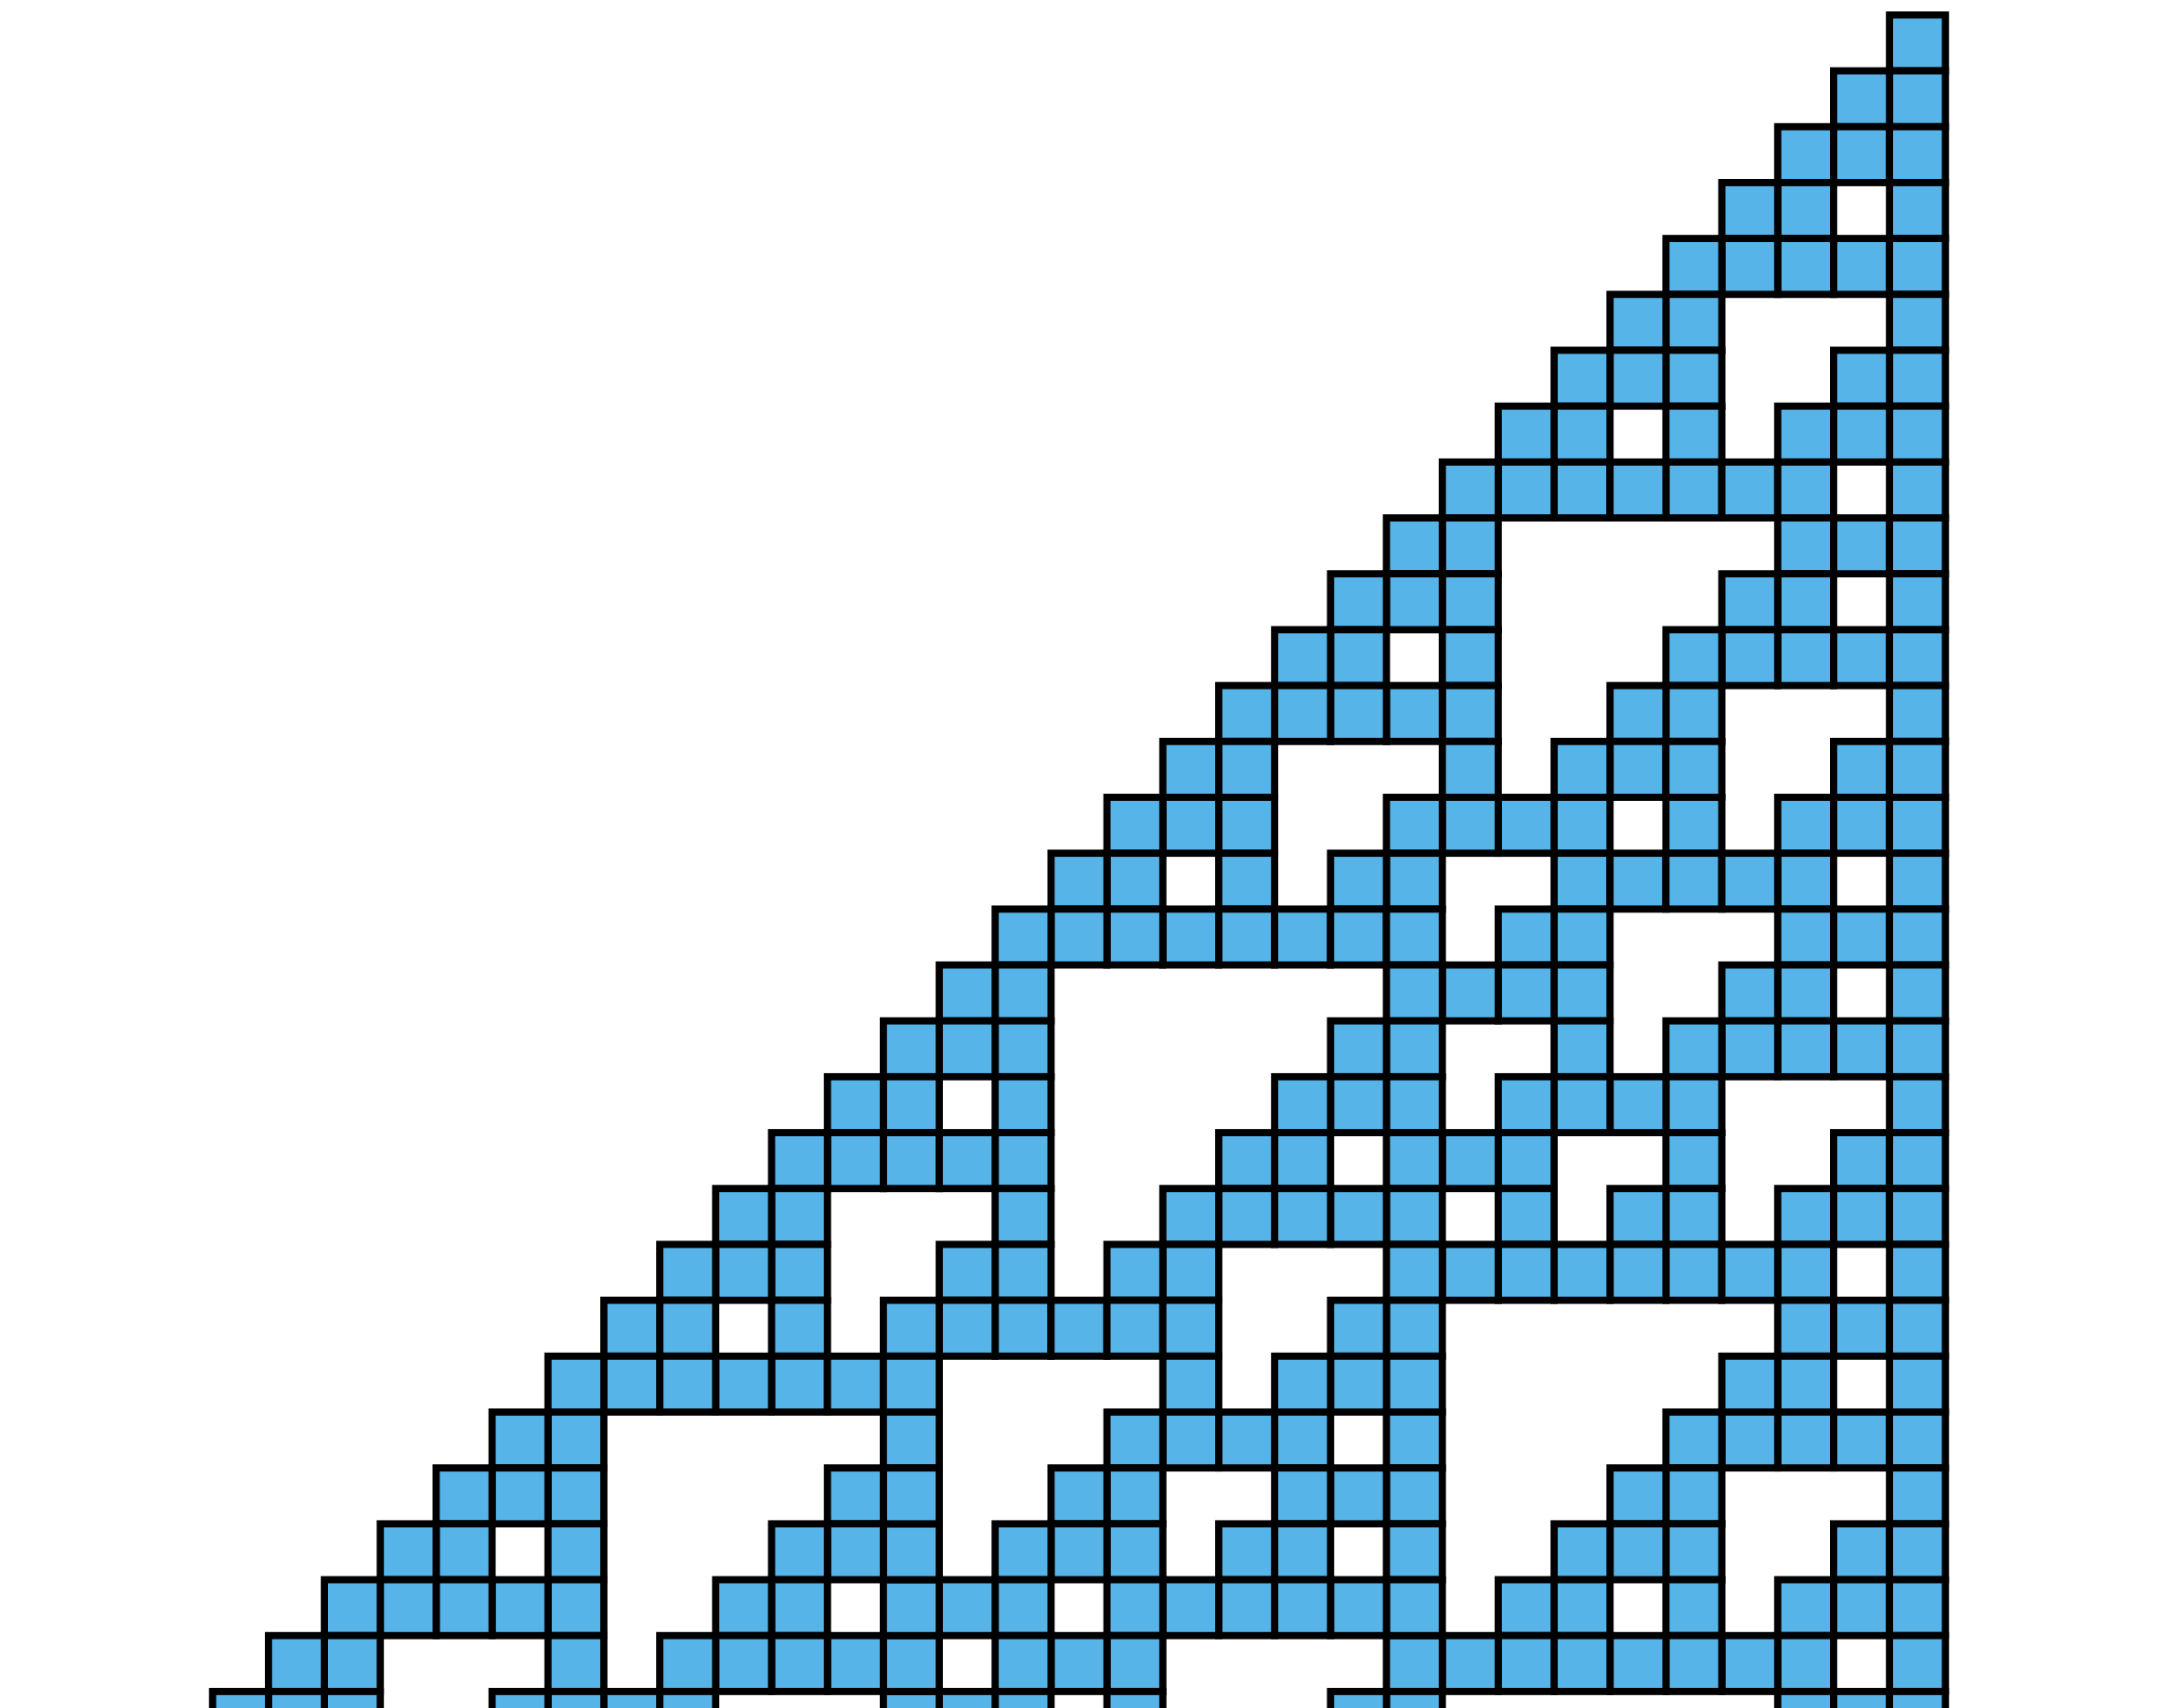
\includegraphics[width=\textwidth]{Figure 5.4.A}
\caption{Elementary Cellular Automaton Rule 110 is Turing Complete}
\end{figure}
\noindent
It may therefore execute or represent any computable function given some initialization.

\section{Simple Stochastic Cellular Automata}
A \textbf{simple stochastic cellular automaton}\index{simple stochastic cellular automaton} is a stochastic cellular automaton in which each cell $x$ in the $d$-dimensional rectangular lattice $X = \mathbb Z^d$ takes on a Boolean value $x \in \{-1, +1\}$. The lattice $X$ evolves over time $t$, $X_t$. Each cell $x$ at time $t$ has a probability distribution that is proportional to its first-order neighbor values:
\begin{figure}[H]
\centering
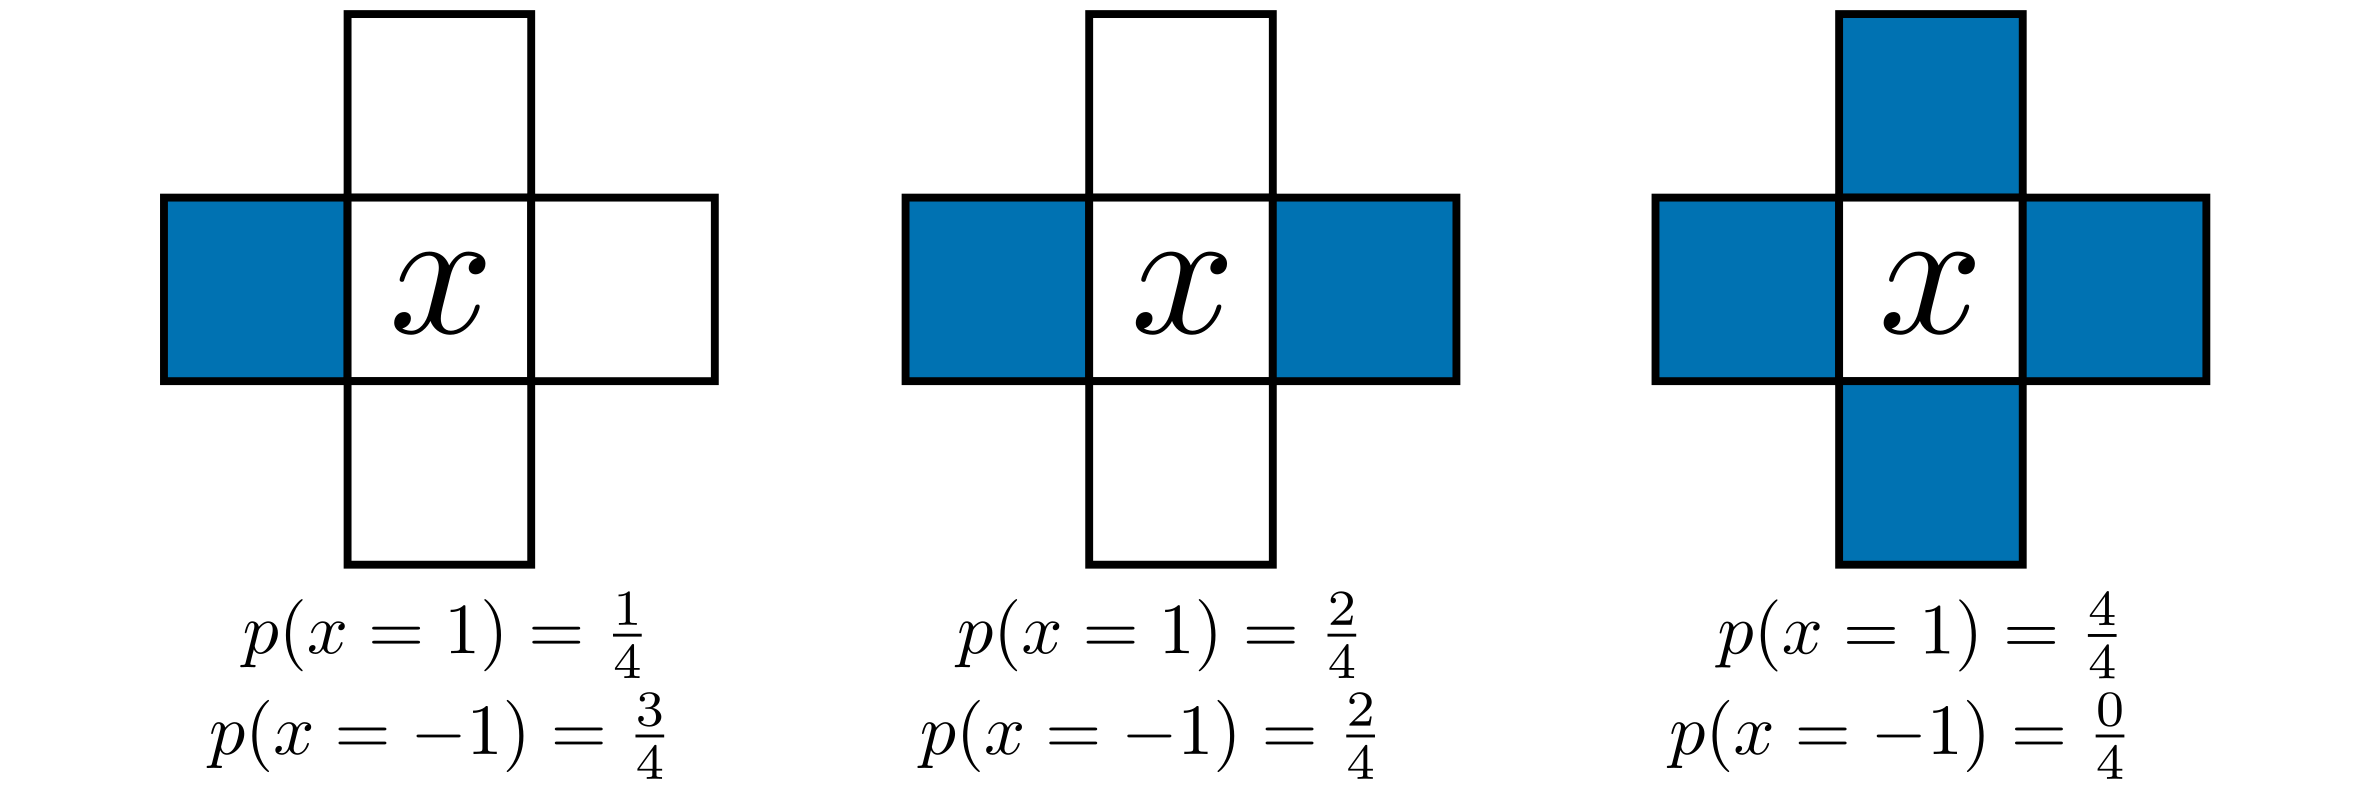
\includegraphics[width=\textwidth]{Figure 5.5.A}
\caption{Transition probabilities depending upon adjacent cells}
\end{figure}
\noindent By itself, this has a fatal flaw since snake/diagonal states have a finite probability to degenerate the whole system $X$ to all values being $-1$ or $+1$:
\begin{figure}[H]
\centering
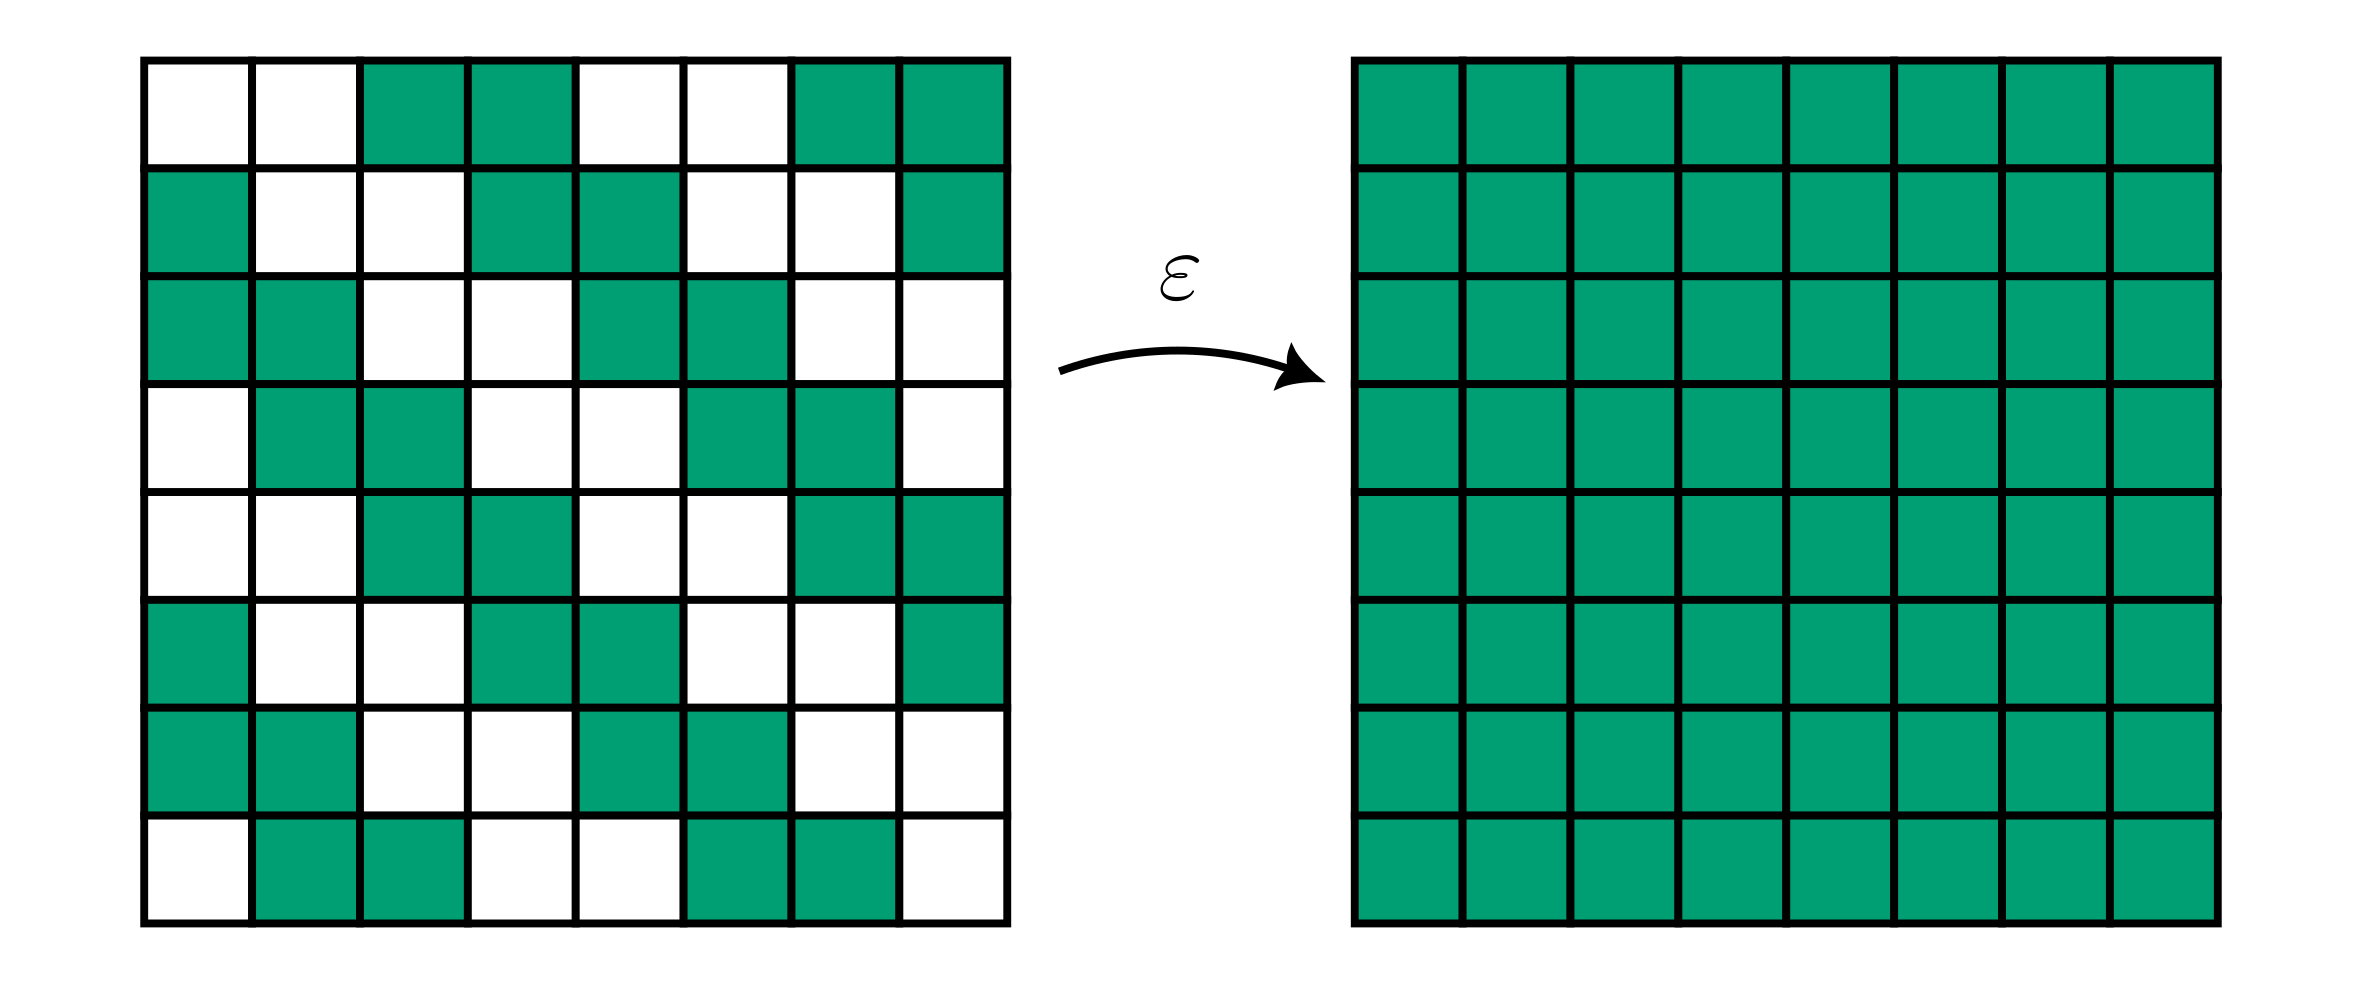
\includegraphics[width=\textwidth]{Figure 5.5.B}
\caption{A snake state may enter a degenerate state with no escape, a Last Judgment state}
\end{figure}
\noindent Alternatively, the checkerboard state purely oscillates if reached:
\begin{figure}[H]
\centering
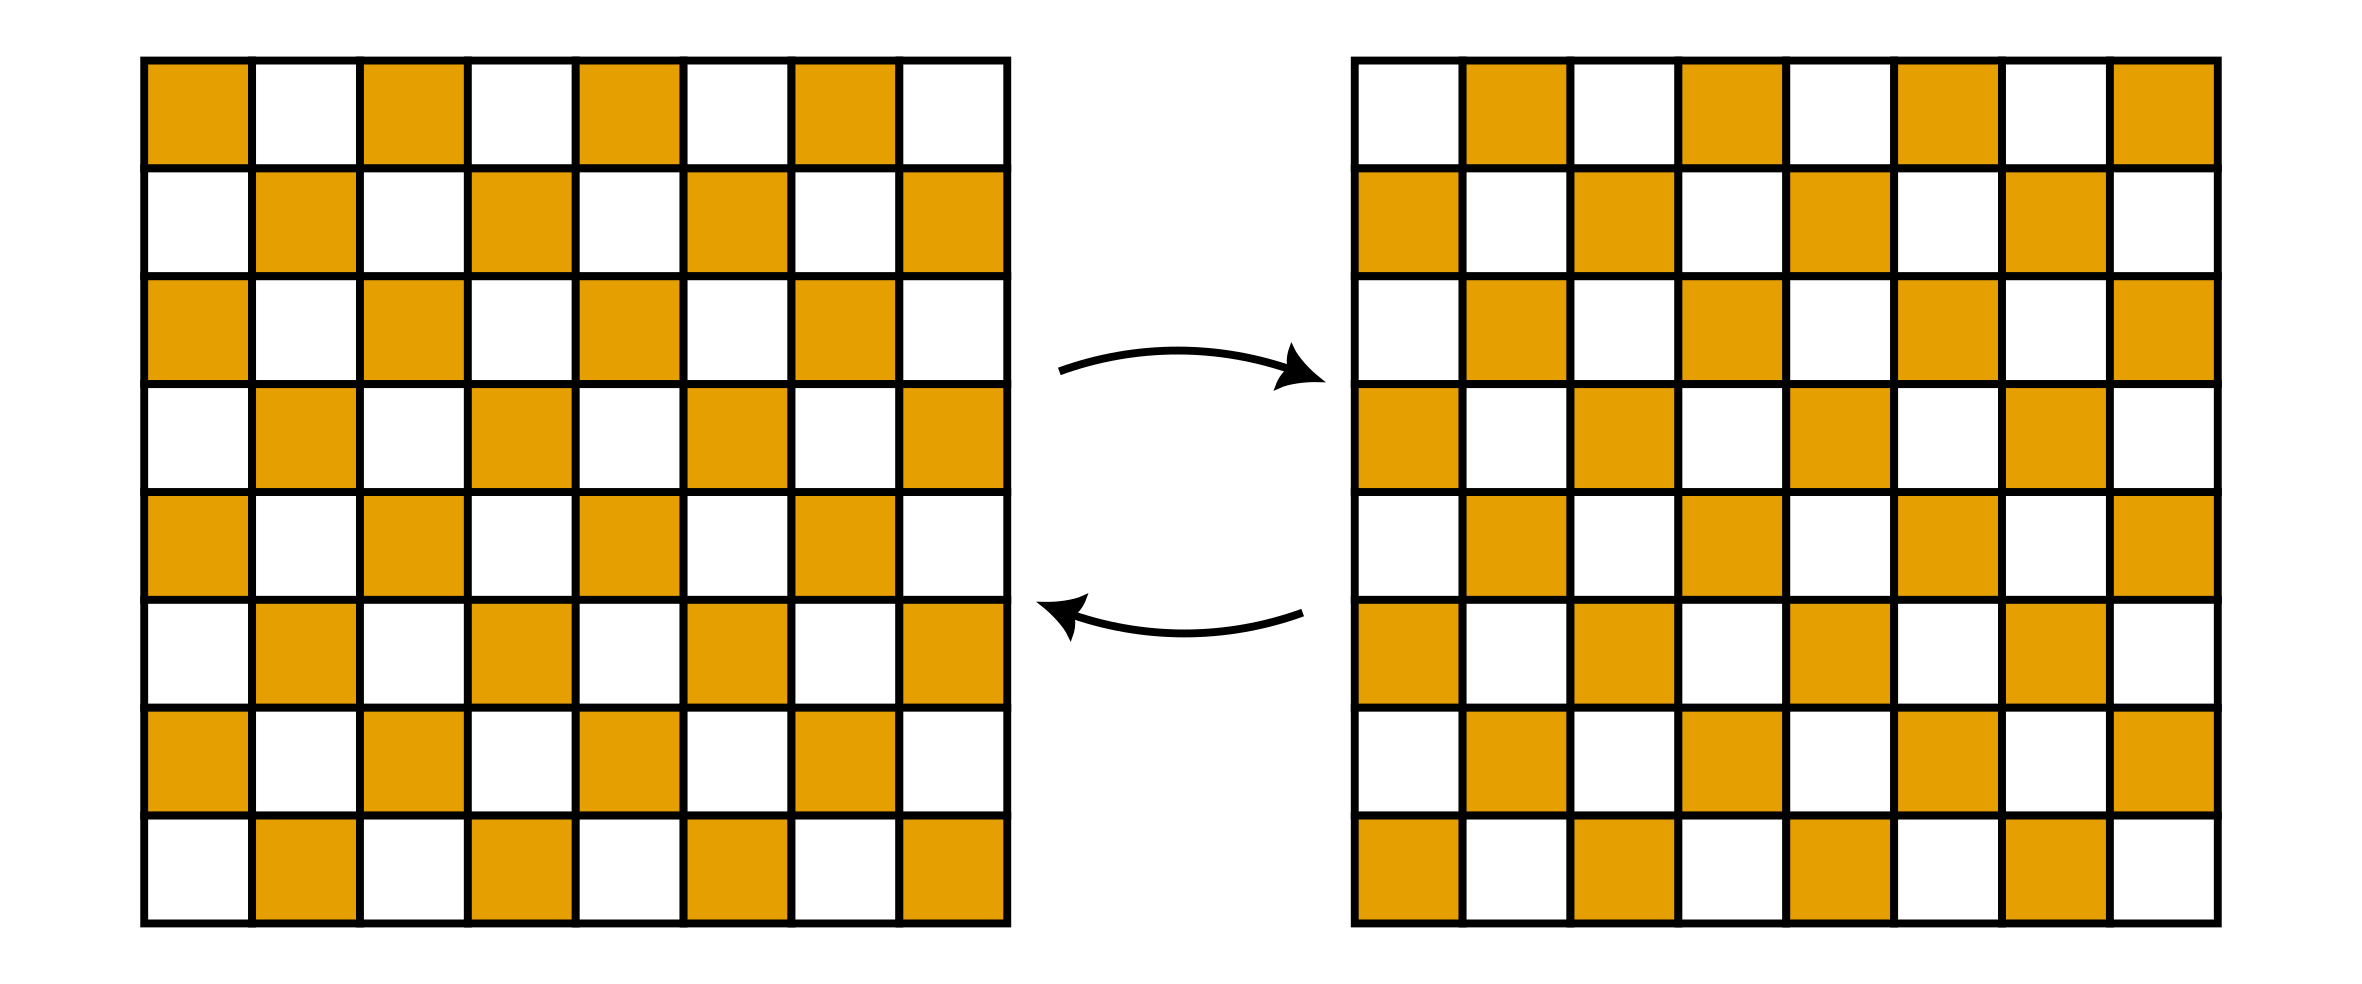
\includegraphics[width=\textwidth]{Figure 5.5.C}
\caption{A checkerboard state is part of a degenerate cycle with no escape}
\end{figure}

In order to prevent degeneracy to deterministic cycles, we need some kind of noise in order to recover from them. Let the external factors $p(x)$ and internal factors $q(x)$ make up the transition function $f(x)$. Let $\varepsilon$ be a constant $\varepsilon \in [0,1]$ that controls the noise of the transition function. Then:
$$f(x) = (1 - \varepsilon)p(x) + \varepsilon q(x)$$
in which $q(x)$ has an equal chance of being $-1$ and $+1$ and $p(x)$ has a $\frac{n}{2d}$ probability of being $+1$ is $x$ has $n$ positive neighbors and likewise a $1-\frac{n}{2d}$ probability of being $-1$.

A noise parameter $\varepsilon$ is assumed to have a critical value of $\varepsilon_{c} = \frac{1}{2}$. Future values of the lattice $X$ are not pure order and not chaos, instead their ideal marriage. These simple cellular automata are similar to the alignment of spins in the Ising model as described in \textit{\S 4.6 Ising Model}. It obeys all the rules of a measure-preserving dynamical system. It is unclear precisely how stable the Markov chain really is, as information of the state may be arbitrarily overwritten or erased. This is unlikely, but it is harrowing to think about if taken as digital physics model of the universe. This is the alternative candidate theory for Boolean mechanics as opposed to Boolean random walks. Boolean random walks is the default candidate for explanation since it neatly ties into concepts of fluid mechanics and differential equations.

\chapter{Boolean Functions}
\section{Motivations for Learning Boolean Functions}

A text on Boolean statistical mechanics would not be complete without a chapter dedicated to Boolean functions. A \textbf{Boolean function}\index{Boolean function} $f(\cdot)$ is a function whose input is $x \in \mathbb B^n$ and output is $f(x) \in \mathbb B^m$ in which the Boolean set is $B_\pm = \{-1, +1\}$. The physical realization or representation of a Boolean function in a system is known as a \textbf{logic gate}\index{logic gate}. This physical realization or representation may be similar to real-life computers or alternative systems like Conway's \textit{Life}.

Alan Turing's paper \textit{On Computable Numbers} moved the world away from human computers to machine computers. The nations with the strongest economies have a strong reliance of cheap and commercially available electronic computers. Smart phones are so widespread that an individual may have more reliable access to radio communication than clean drinking water in the poorest of countries. Applications in which the value of computers is most obvious are accounting, telecommunications, manufacturing, and most importantly documentation. While rendering text may seem like a trivial task, the irony is that the act of arranging an alphabet letters on a page is related to fundamental ideas in computation.

What exactly makes Boolean functions so versatile? First, a Boolean sequence of $n$ bits can represent an alphabet $A$ with cardinality $|A| \leq 2^n$. Second, Boolean functions for any mapping $f: \mathbb B^n \rightarrow \mathbb B^m$ may itself be written as instructions using the Boolean set $\mathbb B$. Often, these instruction $\mathbb B^k$ have a cardinality less than the representations such that $k < m,n$. Third, an infinite extension of $\mathbb B$ can be used to approximate continuous sets and thus continuous functions. Computers, or more formally Turing machines, use these Boolean functions to solve problems that belong to complexity class $R$. The complexity class $R$ refers to the set of \textbf{recursive languages}\index{recursive language}, and it is equivalent to the set of computable functions.

A Boolean random walk may be represented using Boolean functions, but can it represent any Boolean function? A system that can compute every computable function is said to be Turing complete. Any Turing complete system, or Turing machine, may emulate any other Turing complete system. However, a Boolean mechanical system may be probabilistic. \textit{How can we prove or disprove that a Boolean mechanical system is or is not a probabilistic Turing machine?}


\section{AND, OR, \& NOT Functions}
The most simple Boolean functions are of the form $f: \mathbb B^n \rightarrow \mathbb B^1$, having a n-tuple input and a single (or $1$-tuple) output. The Boolean functions AND, OR, \& NOT have the ability to represent any other Boolean function when sequenced together despite having only single outputs. These simple Boolean functions have associated symbols for use in logic diagrams and associated truth tables.

The \textbf{AND function}\index{AND function} takes two inputs $A$ and $B$ and outputs a single value $C$. These form the following AND truth table:
\begin{center}
\begin{tabular}{|c | c | c |}
\hline
$A$ & $B$ & $A \ \textbf{AND} \ B$ \\
\hline
$-1$ & $-1$ & $-1$ \\
$-1$ & $+1$ & $-1$ \\
$+1$ & $-1$ & $-1$ \\
$+1$ & $-1$ & $+1$ \\
\hline
\end{tabular}
\end{center}
The AND function is represented using the following AND symbol in circuit diagrams:
\begin{figure}[H]
\centering
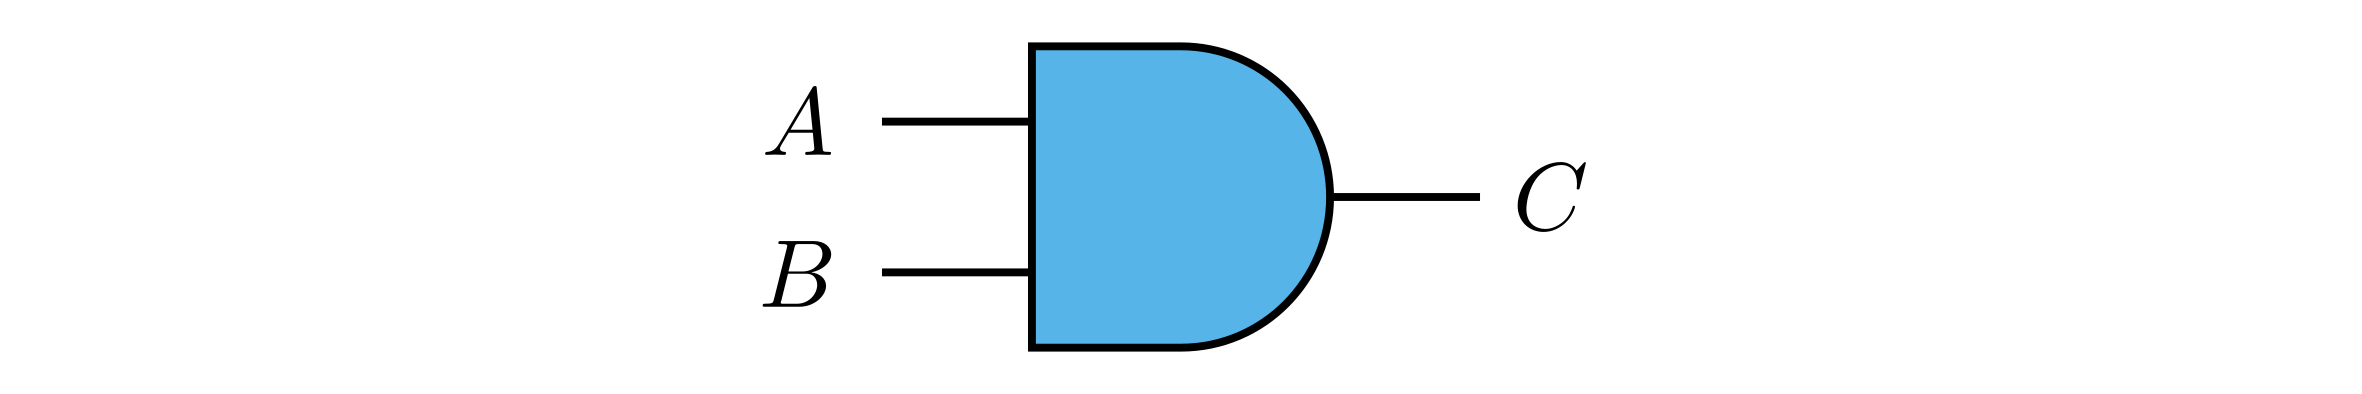
\includegraphics[width=\textwidth]{Figure 6.2.A}
\caption{The AND logic gate representing the AND Boolean function}
\end{figure}
\noindent It may alternatively be considered the \textit{minimum function} for two Boolean inputs.

The \textbf{OR function}\index{OR function} takes two inputs $A$ and $B$ and outputs a single value $C$. These form the following OR truth table:
\begin{center}
\begin{tabular}{|c | c | c |}
\hline
$A$ & $B$ & $A \ \textbf{OR} \ B$ \\
\hline
$-1$ & $-1$ & $-1$ \\
$-1$ & $+1$ & $+1$ \\
$+1$ & $-1$ & $+1$ \\
$+1$ & $-1$ & $+1$ \\
\hline
\end{tabular}
\end{center}
The OR function is represented using the following OR symbol in circuit diagrams:
\begin{figure}[H]
\centering
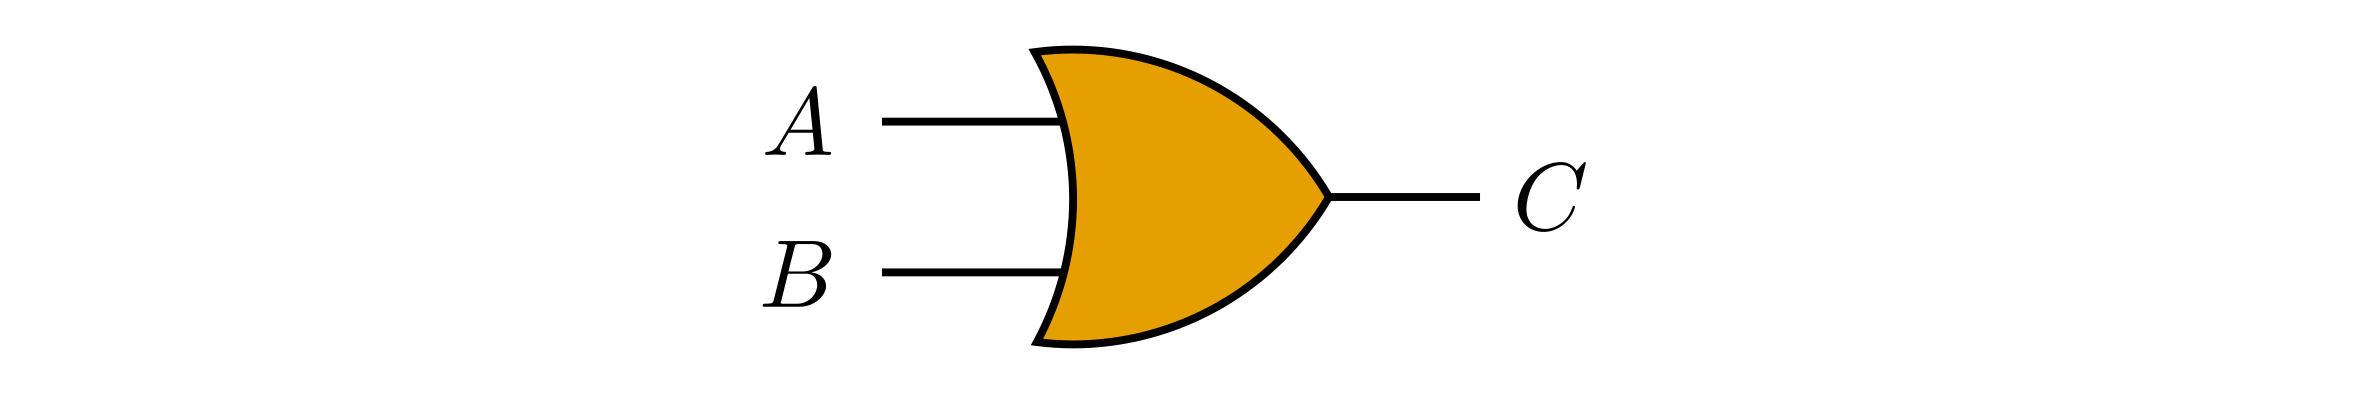
\includegraphics[width=\textwidth]{Figure 6.2.B}
\caption{The OR logic gate representing the OR Boolean function}
\end{figure}
\noindent It may alternatively be considered the \textit{maximum function} for two Boolean inputs.

The \textbf{NOT function}\index{NOT function} takes a single input $A$ and outputs a single value $C = -A$. More generally, we say that it returns the Boolean complement of $A$. The NOT function has the following truth table:
\begin{center}
\begin{tabular}{|c | c |}
\hline
$A$ & $\textbf{NOT} \ A$ \\
\hline
$-1$ & $+1$ \\
$-1$ & $+1$ \\
\hline
\end{tabular}
\end{center}
The NOT function is represented using the following NOT symbol in circuit diagrams:
\begin{figure}[H]
\centering
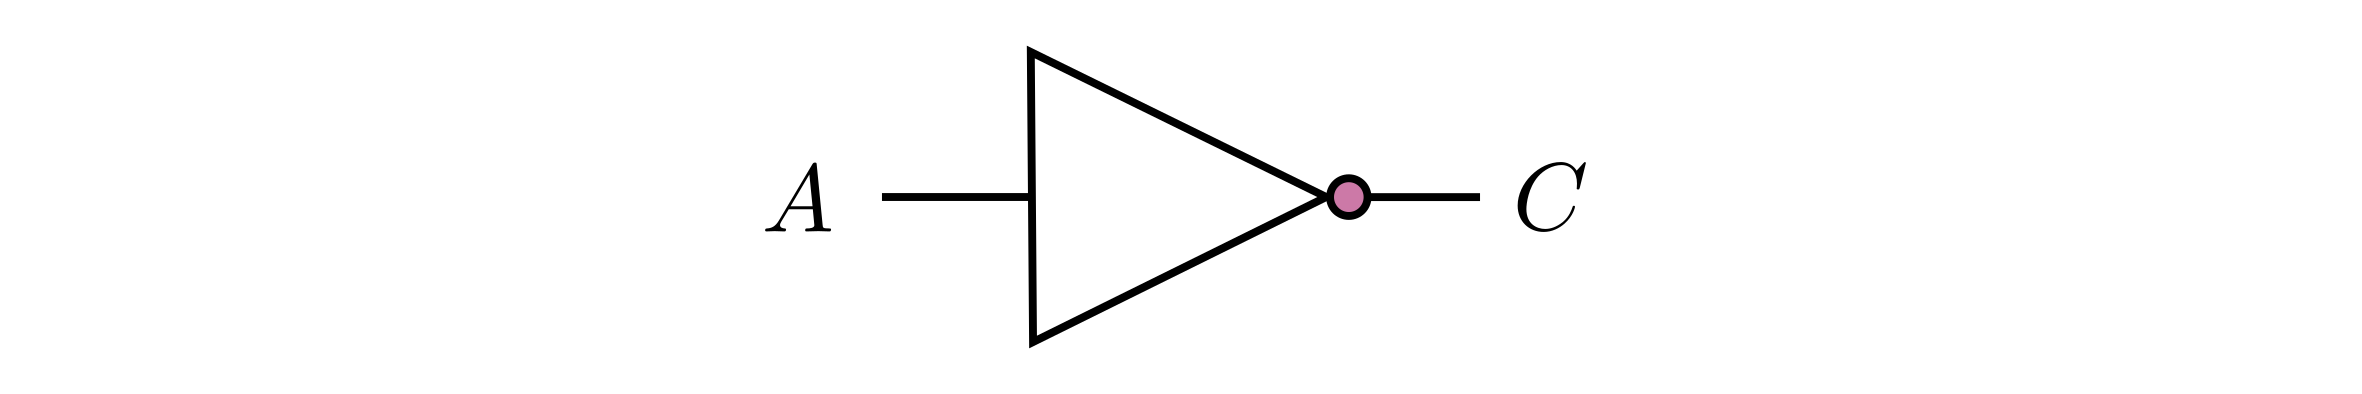
\includegraphics[width=\textwidth]{Figure 6.2.C}
\caption{The NOT gate inverts the Boolean signal}
\end{figure}
\noindent It may alternatively be referred to as the negation or complement function for $f: \mathbb B^n \rightarrow \mathbb B^n$. Any function $f(\cdot)$ is said to be an \textbf{odd function}\index{odd function} if:
$$f(-A) = -f(A) \iff f(A) = -f(-A)$$
or negating the inputs is equal to negating the outputs. This is related to the previously discussed idea of dichromatic symmetry.

The logic symbols can be arranged to form a circuit diagram like so:
\begin{figure}[H]
\centering
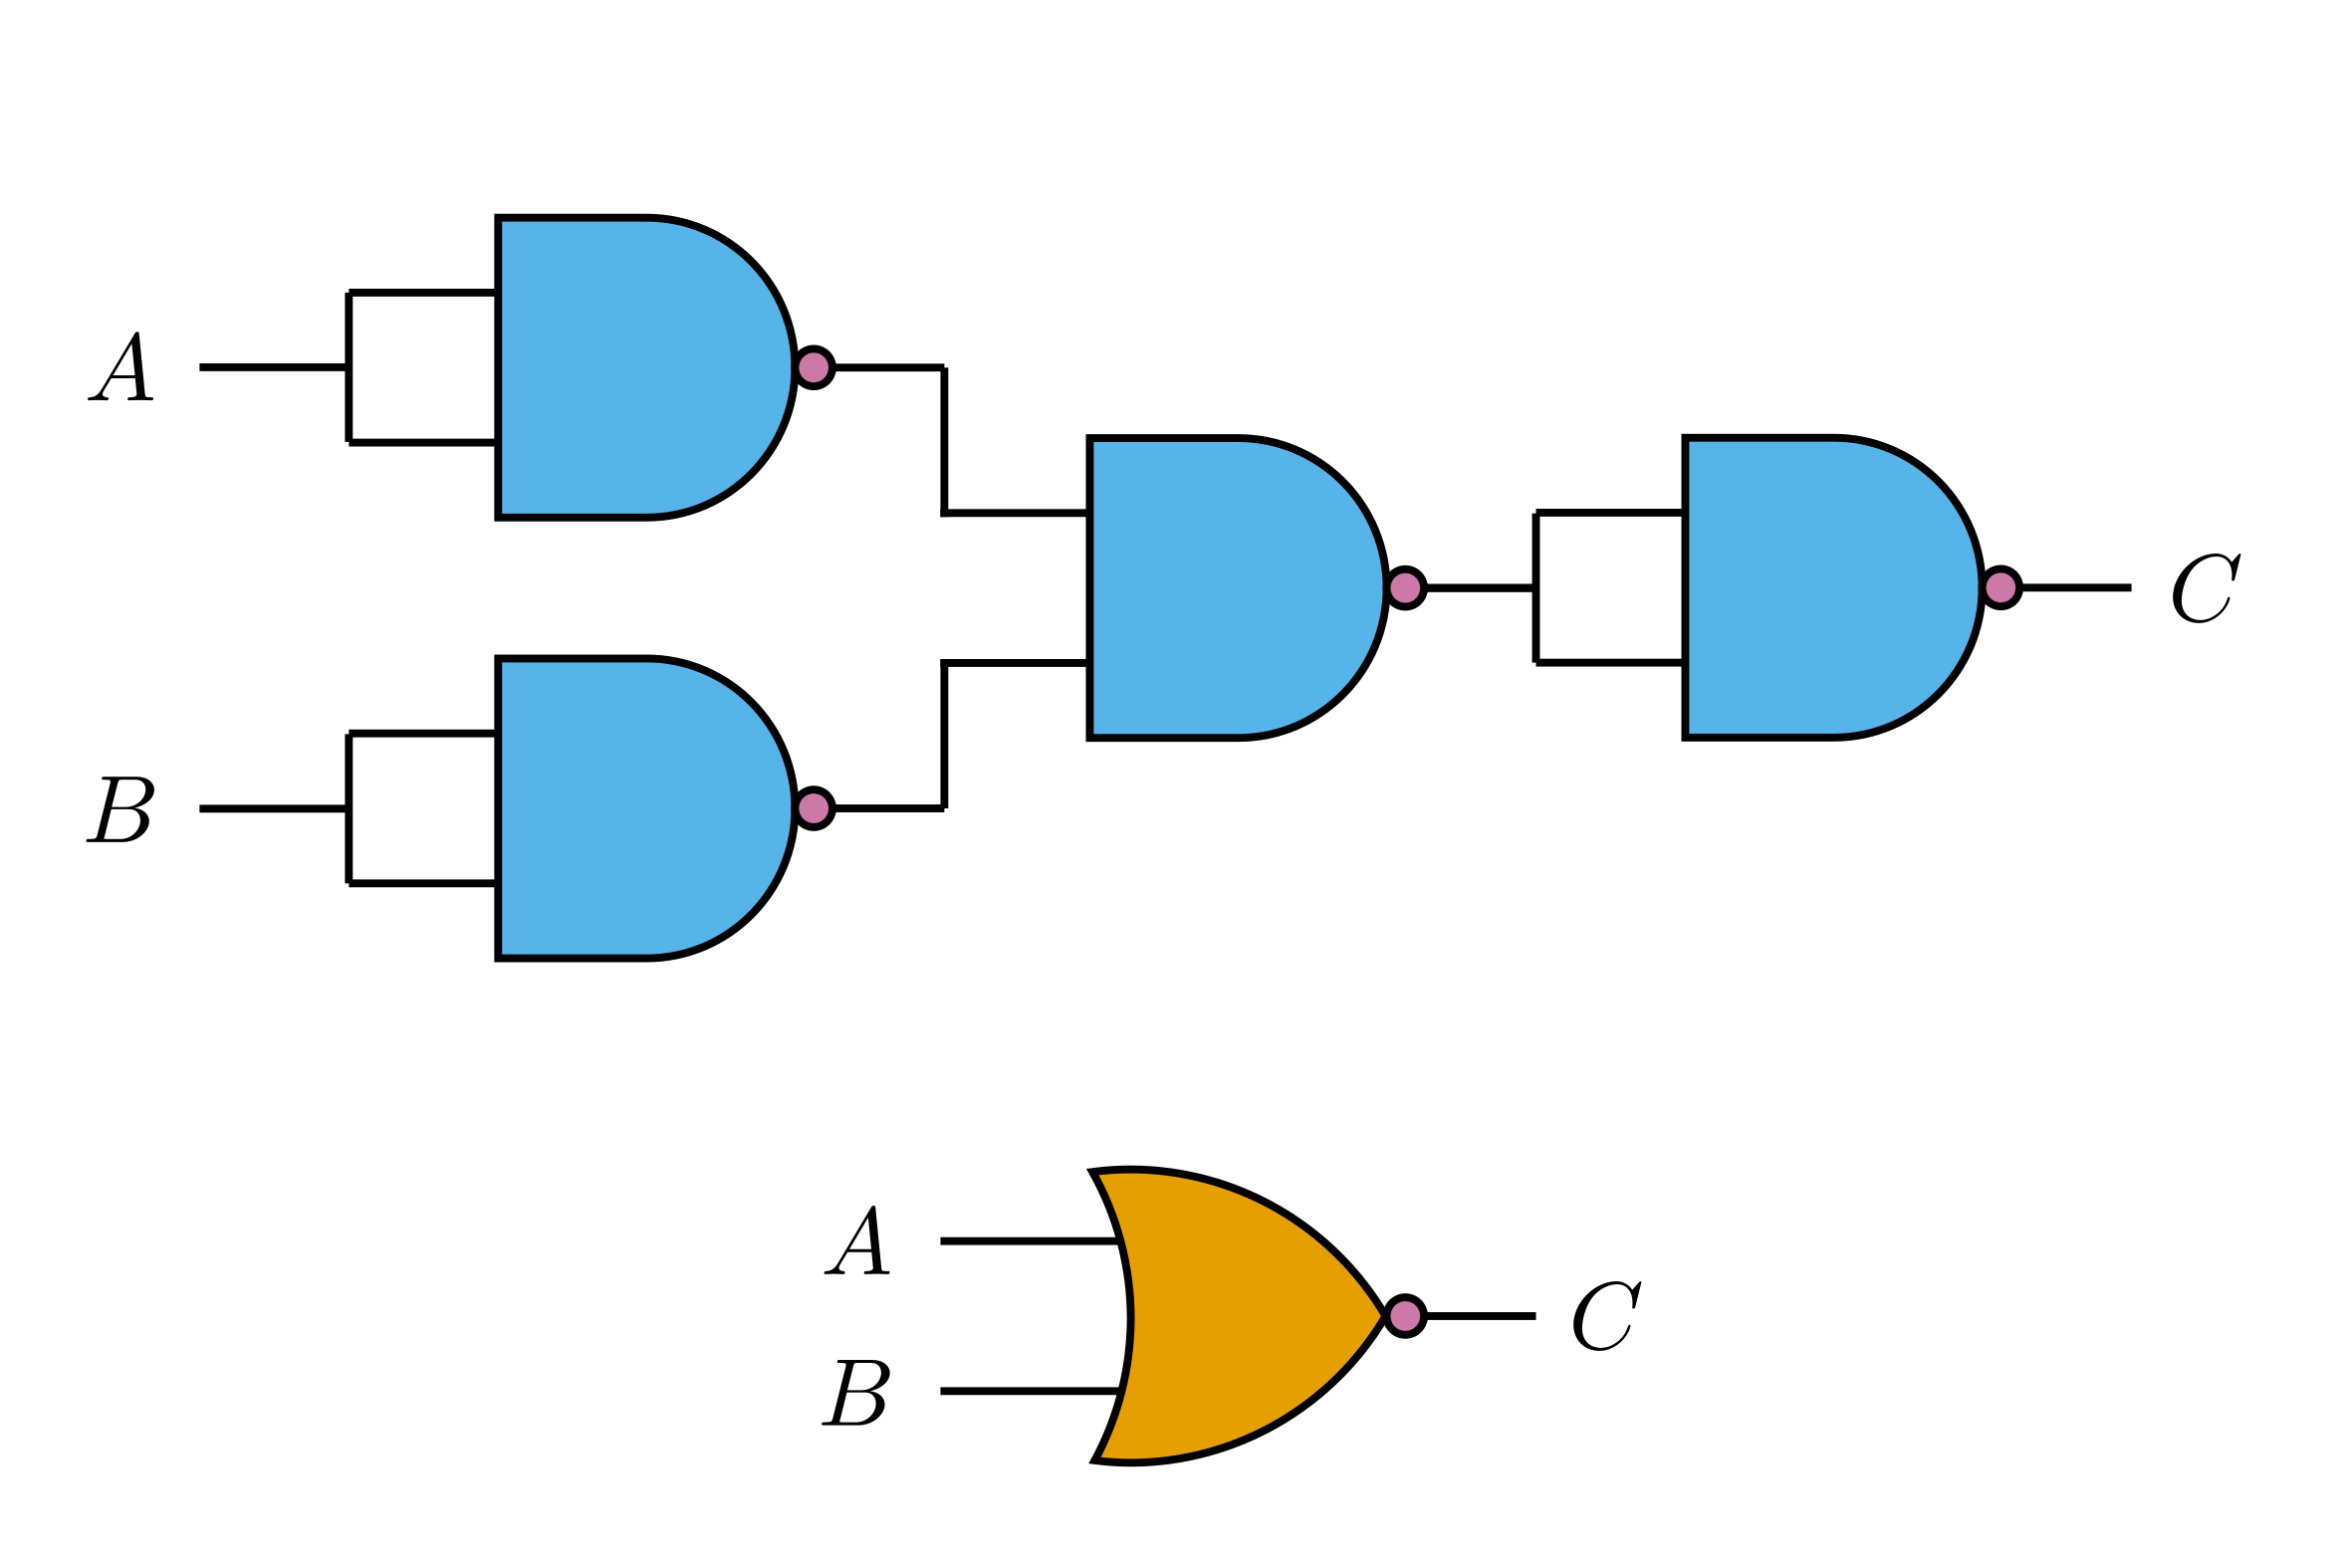
\includegraphics[width=\textwidth]{Figure 6.2.D}
\caption{A sequence of NAND gates imitating a NOR gate}
\end{figure}
\noindent This diagram is a NOR, or NOT-OR, Boolean function emulated using NOT-AND chains. The NAND and NOR gates inherit the properties of NOT gates by inverting the output.

Together, these simple Boolean functions can construct any multiple input, multiple output Boolean function $f: \mathbb B^n \rightarrow \mathbb B^m$. A \textbf{computable function}\index{computable function} is any function that maps a natural number to a Boolean value:
$$f: \mathbb N \rightarrow \mathbb B$$
This essentially means that a computable function is equivalent to assigning a ``Boolean class'' to each natural number. We say that if a function is computable, then it belongs to the set of all functions from the natural numbers to the Boolean set:
$$f \in \mathbb{N}^{\mathbb B}$$
since it can decide on a value for each input. Computable function does not specify the amount of time, but it does guarantee that the time is finite for a specific input. Computable function does not specify the amount of space, but it does guarantee that the space is finite for a specific input. Computable does not mean efficiently computable or practically computable with the number of electrons in the observable universe.

It does mean that there is a finite algorithm that generates the Boolean value. For example, the odd numbers are a computable function. It would take an infinite amount of time and space to enumerate every odd number, but the length of the \textit{instructions} to determine if a single input is odd is \textit{finite}. It follows that the length of the \textit{runtime} to determine if a single input is odd is \textit{finite}. There are functions that are not computable, that are not decidable for every input. The key example of a non-computable problem the \textbf{halting problem}\index{halting problem}, or using a finitely written program to determine if any other program performs an infinite loop or will halt.

A \textbf{computably enumerable function}\index{computably enumerable function} is any function that maps a non-empty proper subset $N$ of the natural numbers $\mathbb N$ to a Boolean value $\mathbb B$:
$$f: N \rightarrow \mathbb B, \ N \subset \mathbb N, \ N \neq \varnothing$$
A computably enumerable function is also a Boolean classifier with a finite domain of inputs. If the function $f$ takes an input not from the domain $N$, then it is not guaranteed to halt by providing an output value. The function may loop forever without producing an output in the case of an invalid input.

The fact that Boolean functions can represent each other presents a fundamental arbitrariness. Suppose you have a cellular automata, and it can represent Boolean functions with physically manifested logic gates in the universe. If inverting the Boolean inputs simultaneously switches all NAND-like objects with NOR-like objects, then the transition function is an odd function.
\begin{figure}[H]
\centering
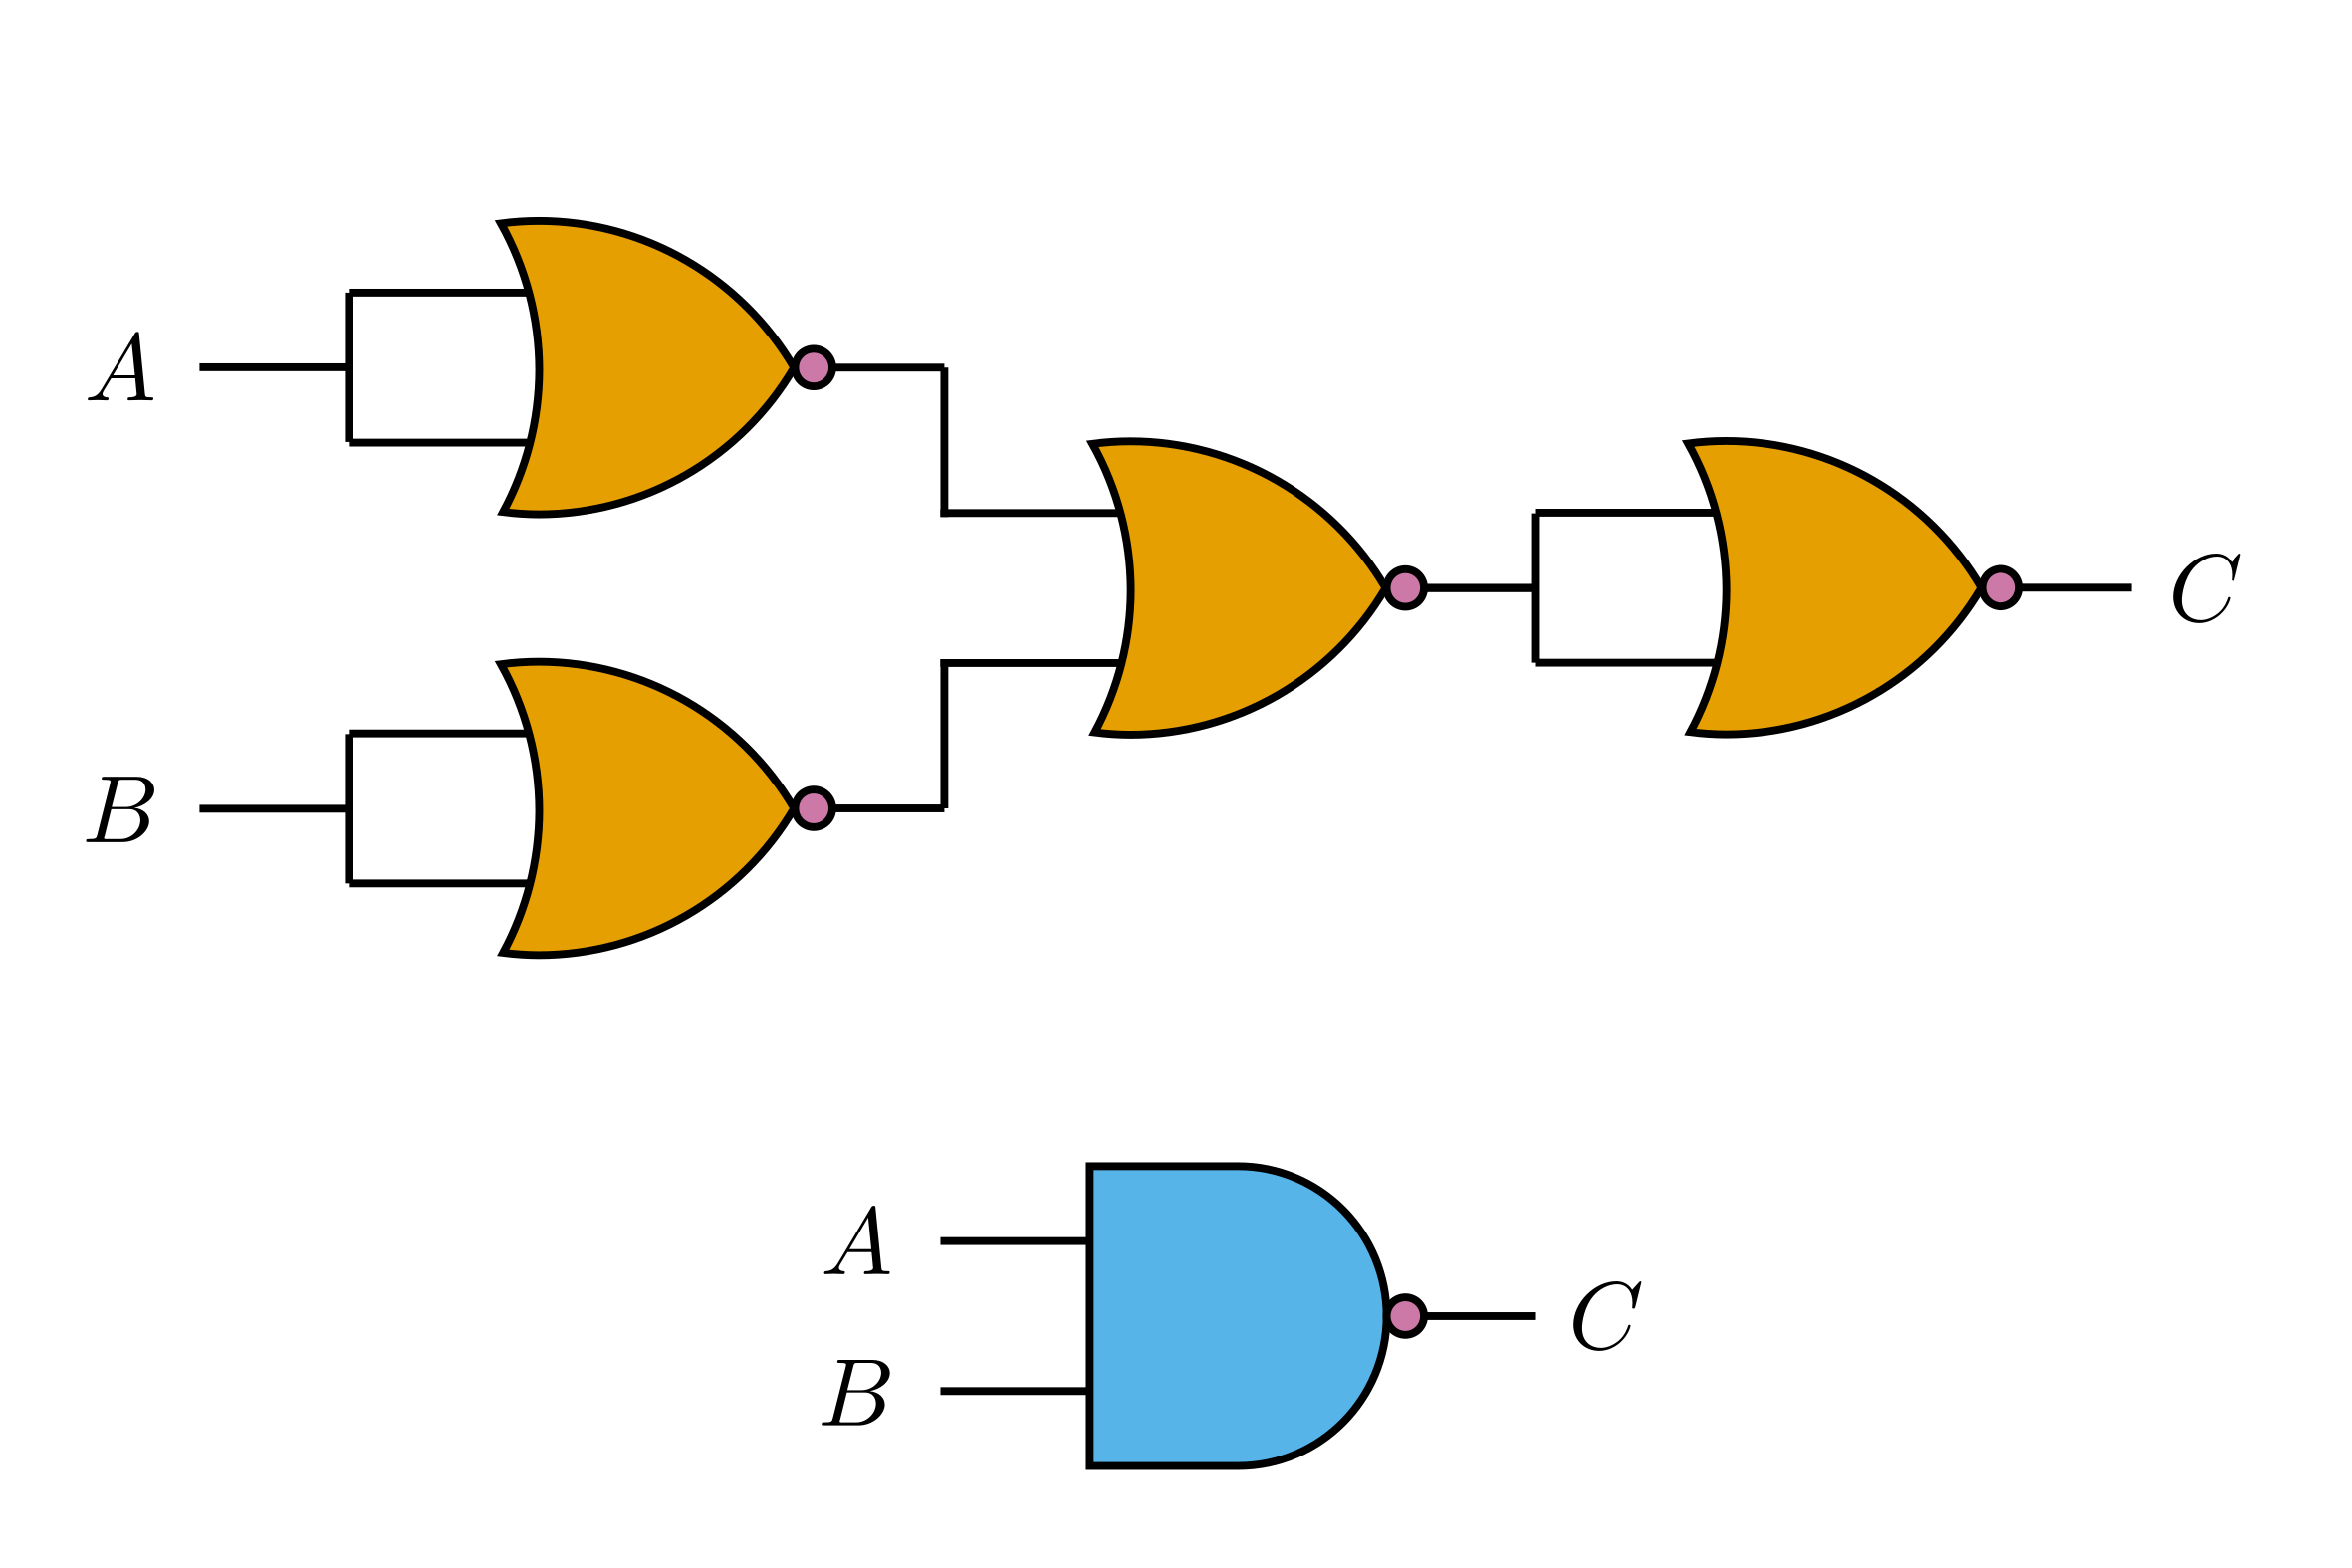
\includegraphics[width=\textwidth]{Figure 6.2.E}
\caption{A sequence of NOR gates imitating a NAND gate}
\end{figure}
\noindent 
This diagram is a NOR, or NOT-OR, Boolean function that is emulated using NOT-AND chains. The difficulty is in finding a cellular automata or computable universe with an odd transition function that is Turing complete. The Rule 110 Elementary Cellular Automata is Turing complete, but it is not an \textit{odd} transition function. How can we discover odd transition functions for the universe are that computable and can compute any other object? We will need to discuss functional completeness.

\section{NAND \& NOR Functional Completeness}
The Boolean functions NAND \& NOR are each \textbf{functionally complete}\index{functional completeness}. A functionally complete set of operations can represent any other Boolean function. The set $\{\textnormal{NAND}\}$ is functionally complete, the set $\{\textnormal{NOR}\}$ is functionally complete, the set $\{\textnormal{AND, OR, NOT}\}$ is functionally complete, and the set $\{\textnormal{AND, OR}\}$ is incomplete. Any computable function of complexity class $R$ can be represented using constructions of a functionally complete set.

The following are the circuit diagram representations of NAND and NOR respectively:
\begin{figure}[H]
\centering
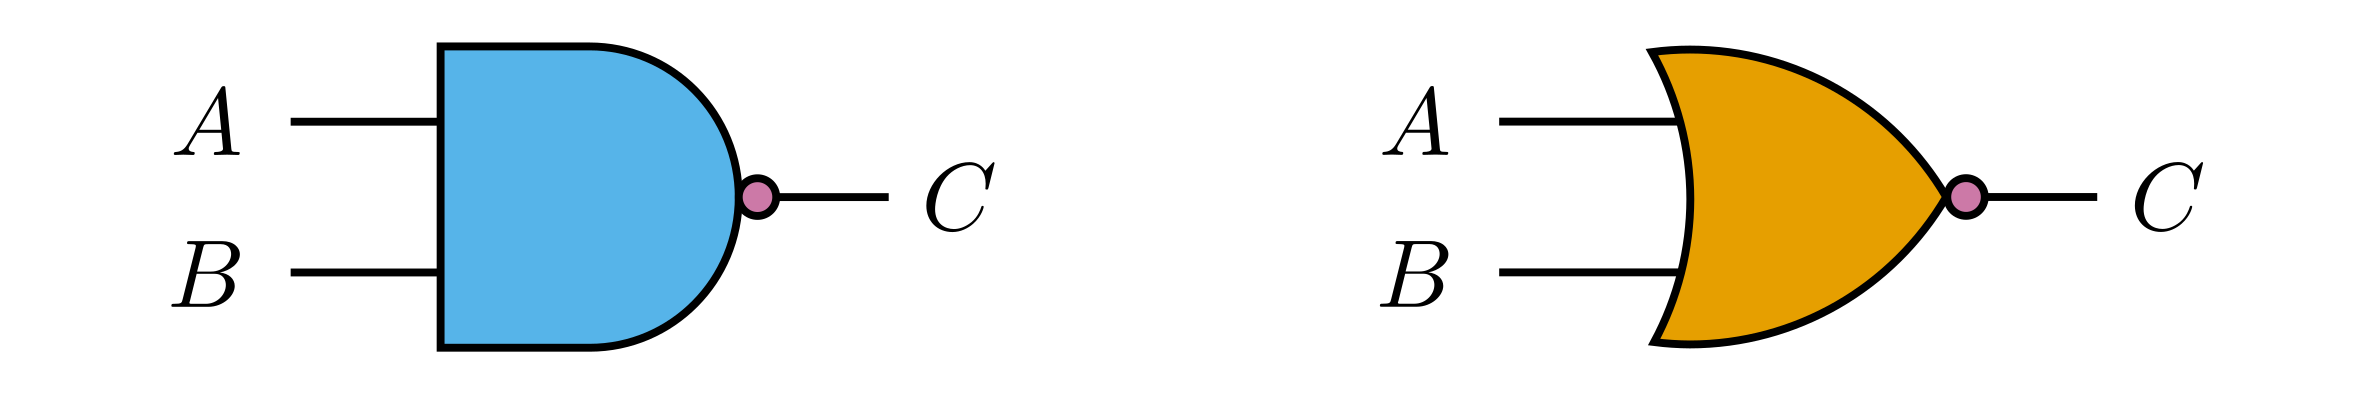
\includegraphics[width=\textwidth]{Figure 6.3.A}
\caption{NAND gate on the left, NOR gate on the right}
\end{figure}
\noindent
These is the truth table of NAND:
\begin{center}
\begin{tabular}{|c | c | c |}
\hline
$A$ & $A \ \textbf{NAND} \ B$ & B\\
\hline
$-1$ & $+1$ & $-1$ \\
$-1$ & $+1$ & $+1$ \\
$+1$ & $+1$ & $-1$ \\
$+1$ & $-1$ & $+1$ \\
\hline
\end{tabular}
\end{center}
and this is the truth table of NOR:
\begin{center}
\begin{tabular}{|c | c | c |}
\hline
$A$ & $A \ \textbf{NOR} \ B$ & B\\
\hline
$-1$ & $+1$ & $-1$ \\
$-1$ & $-1$ & $+1$ \\
$+1$ & $-1$ & $-1$ \\
$+1$ & $-1$ & $+1$ \\
\hline
\end{tabular}
\end{center}

We know that $\{\textnormal{AND, OR, NOT}\}$ denote a functionally complete set. How do we know that a Boolean random walk is functionally complete? Considering the following 1D systems that are bound at the edges:
\begin{figure}[H]
\centering
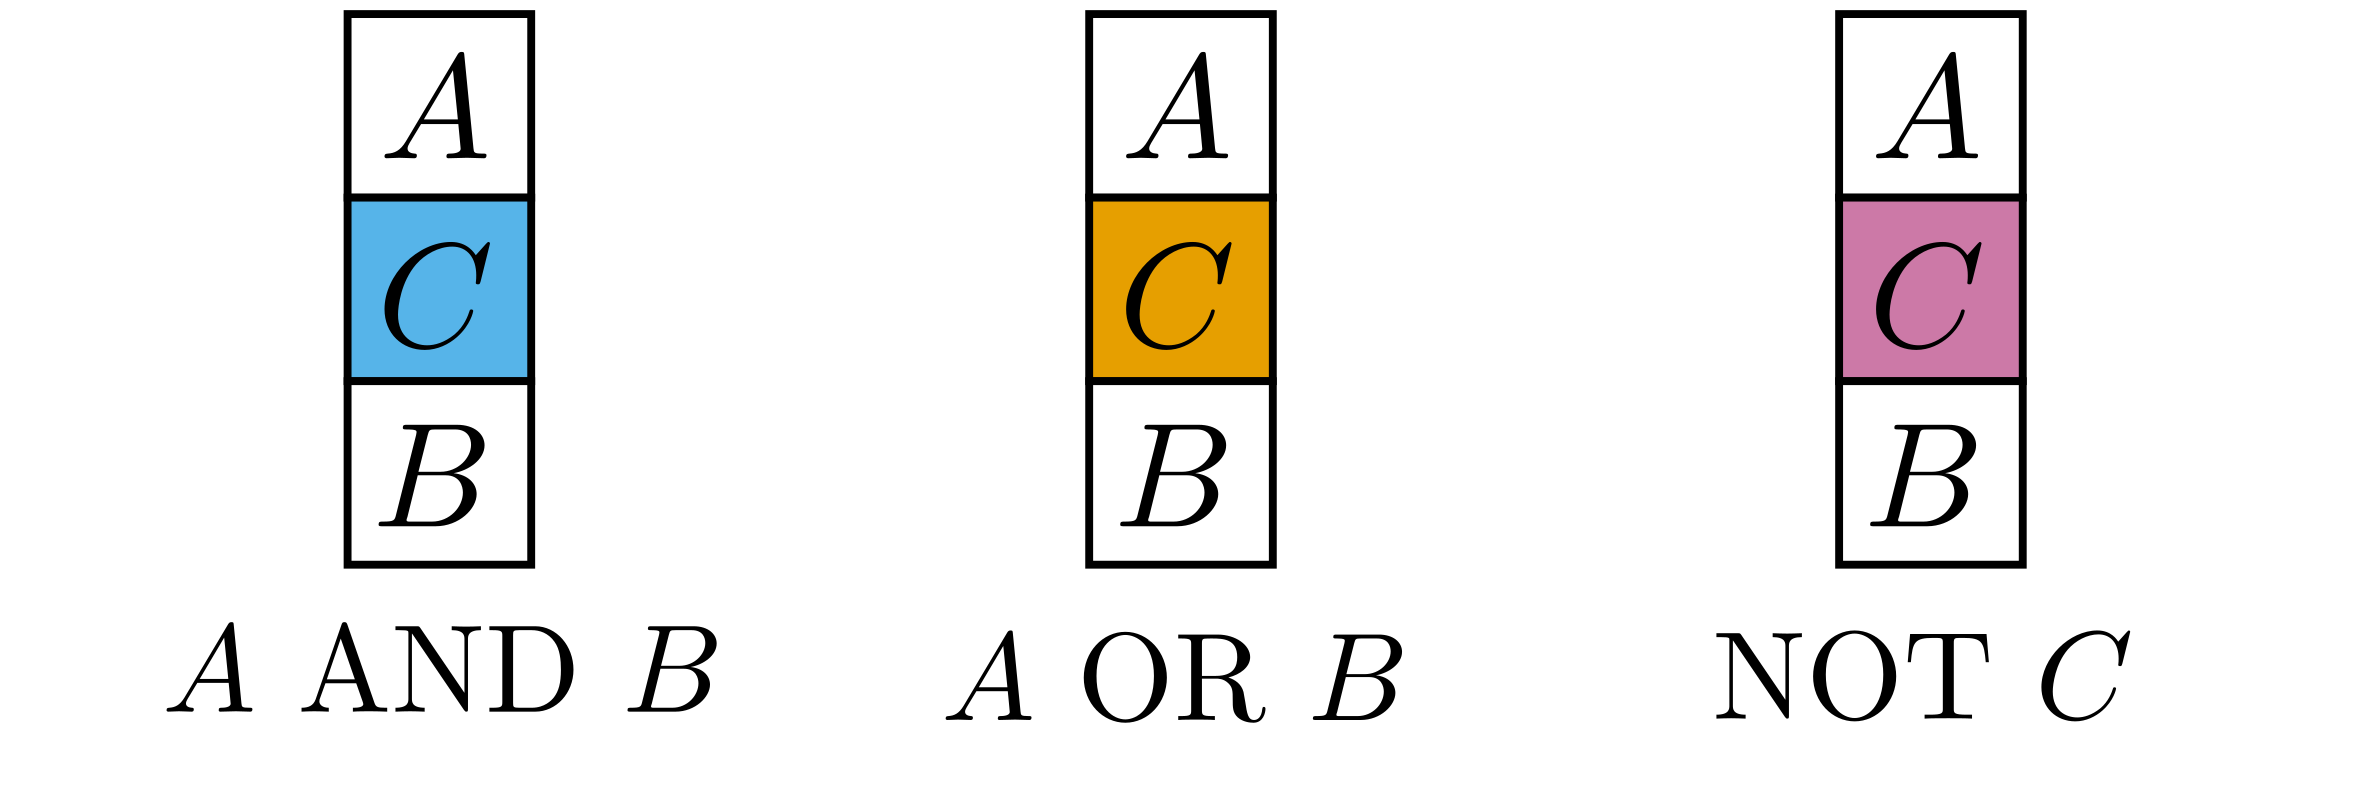
\includegraphics[width=\textwidth]{Figure 6.3.B}
\caption{The functional completeness of a Boolean random walk}
\end{figure}
\noindent If we begin the simulation at time $t$, the Boolean operation $A \ \textnormal{AND} \ B$ occurs on $C_{t+1}$ if $C_t = +1$. Likewise, the Boolean operation $A \ \textnormal{OR} \ B$ occurs on $C_{t+1}$ if $C_t = -1$. The Boolean operation $\textnormal{NOT} \ C$ occurs on $C_{t+1}$ if $A_t = +1, B_t = -1$. This is true regardless of the resolution order in which the Boolean random walk evolves.

If we add more cells around the edges and increase the dimensionality, the probability that the represented Boolean function may occur \textit{decreases}. This is due to interference latent in a Boolean random walk, so not every cell experiences a derangement. The derangement probability depends on the density and the dimensionality of the Boolean random walk.

Compared to our regular circuit diagram notation, it is very difficult to control and predict the future of a Boolean random walk. We cannot construct something that will behave how we like to be a deterministic function. The assumption is that initializing via a Bernoulli random field will settle into something that is self-regulating with some probability. We discuss the nature of probabilistic logic in the next section.


\section{Probabilistic Logic and Linear Combinations}
A \textbf{probabilistic Boolean function}\index{probabilistic Boolean function} is a Boolean function $f: \mathbb B^n \rightarrow \mathbb B^m$ with a random output. The randomness requirement is rather loose as is the probability distribution on the possible output from $\mathbb B^m$ of non-zero entropy for some input $x$, not all inputs. We may use Bayes rule to obtain a distribution on $x$ for a given fixed $f(x)$, similar to matrix inversion of a transition matrix. Since NAND \& NOR are each functionally complete, any probabilistic Boolean function can be written as a linear combination of various sequences of NAND or NOR functions.

A probabilistic Boolean function $F(\cdot)$ composed of many deterministic Bernoulli probability distribution functions $(f_1,...,f_k)$ is of the form:
$$ F(x) = \sum\limits_{j=1}^k p_j f_j(x)$$
Each of the $k$ deterministic Boolean functions $(f_1,...,f_k)$ are of the form $f: \mathbb B^n \rightarrow \mathbb B^m$. To define $F$, each Boolean function $f_j$ that compose $F$ is sampled according to probability $p_j$ in which:
$$ \sum\limits_{j=1}^k p_j = 1$$
Defining the probabilistic Boolean function $F$ this way ensures that each output of the truth table obeys Kolmogorov's axioms of probability. If $(f_1,...,f_k)$ are arbitrary probability distributions, then $F$ is called a \textbf{mixture distribution}\index{mixture distribution}. It also emphasizes that all probabilistic Boolean functions are constructible from Boolean functions of complexity class $R$. In simplest terms, $F$ defines for each input Boolean $n$-tuple some probability distribution for the output Boolean $m$-tuple.

If defined this way, we have a stochastic transition matrix $P_{n \times k}$ that maps all $2^n$ possible Boolean inputs to all $k$ Boolean functions. We shall call the input domain $\mathcal X_n = \mathbb B^n$ and the output codomain $\mathcal X_k = f_{\mathbb B}$. Each row $P_{(i, \cdot)}$ obeys:
$$ \sum\limits_{j=1}^k p_{(i, j)} = 1$$
This stochastic matrix definition of a probabilistic Boolean function is best used if constructing from known Boolean functions. Here is an example transition matrix using NAND and NOR:
\begin{center}
\begin{tabular}{|c || c | c |}
\hline
$x$ & $p_\textbf{NAND(x)}$ & $ p_\textbf{NOR(x)}$\\
\hline
$(-1, -1)$ & 0.3 & 0.7\\
$(-1, +1)$ & 0.4 & 0.6\\
$(+1, -1)$ & 0.6 & 0.4\\
$(+1, +1)$ & 0.2 & 0.8\\
\hline
\end{tabular}
\end{center}
This particular example has a different probability of sampling $f_1$ or $f_2$ depending on the current input. It doesn't particularly matter that $f_1$ or $f_2$ are since any Boolean function of the form $f: \mathbb B^2 \rightarrow \mathbb B^1$ will do. We prefer the following definition for a probabilistic Boolean function instead.

The stochastic transition matrix $P_{n \times m}$ of a probabilistic Boolean function $f:\mathbb B^n \rightarrow \mathbb B^m$ maps all $2^n$ possible Boolean inputs to all possible $2^m$ possible Boolean outputs. We shall call the input domain $\mathcal X_n = \mathbb B^n$ and the output codomain $\mathcal X_m = \mathbb B^m$. Each row $P_{(i, \cdot)}$ obeys:
$$ \sum\limits_{j=1}^m p_{(i, j)} = 1$$
This stochastic matrix definition of a probabilistic Boolean function is the most general, and it is best used for unknown Boolean functions. In fact, a convex linear combination of stochastic matrices:
$$\sum\limits_{j=1}^{k} \omega_j P_j = P^*; \quad \sum\limits_{j=1}^k \omega_j=1; \quad \omega_j \geq 0 \quad \forall j$$
is itself a stochastic matrix $P^*$. 

This strength of this definition is also the exact definition of the transition matrix of a Markov chain. Here is an example transition matrix that contains only probabilities:
$$P = 
\begin{bmatrix}
0 & 1 & 0 & 0 \\
\frac{1}{2} & 0 & \frac{1}{2} & 0\\
0 & \frac{1}{2} & 0 & \frac{1}{2}\\
0 & 0 & 1 & 0
\end{bmatrix}
$$
This definition is superior as we may easily consider the $t$-th iteration of a probabilistic Boolean function $f:\mathbb B^n \rightarrow \mathbb B^n$ using matrix power notation $P^t$. 


Consider a bounded Boolean random walk system $X$ at time $t=0$, $X_0$. We subdivide its regions into a tuple $(A, B, C, F)$:
\begin{figure}[H]
\centering
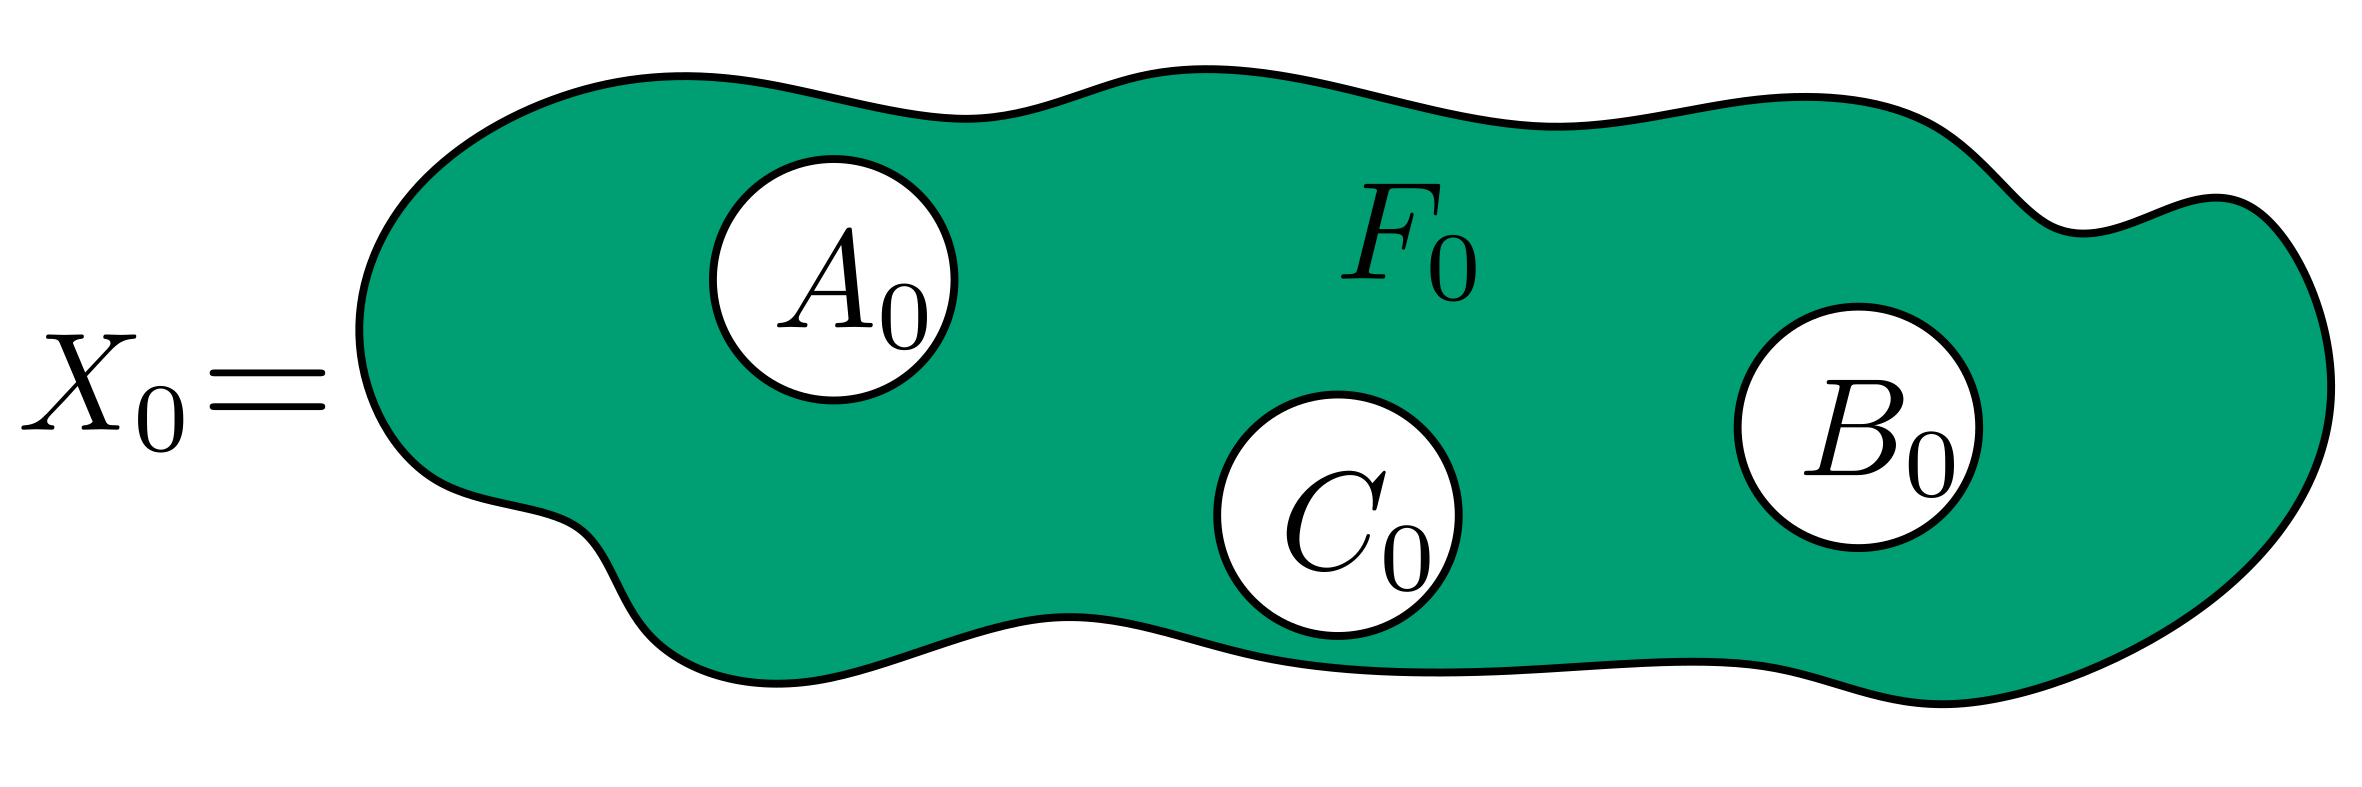
\includegraphics[width=\textwidth]{Figure 6.4.A}
\caption{An abstraction of a cellular automaton's region $F$ acting as a two input function upon $C$}
\end{figure}
\noindent We consider $C_t$ to be the output region measured at time $t$, $A_0$ and $B_0$ to be the input region. We consider $C_0$ and $F_0$ to be the evaluating function. For any arbitrary region $R$, any random ``roll'' of the future region $R_t$ is a Boolean tuple of the same cardinality of the initial region $R_0$:
$$R_t \in \mathbb B^{|R_0|}$$
In fact, it is true for the whole system $X$ that $X_t \in \mathbb B^{|X_0|}$.

We do not state that $F_0$ is the evaluating function alone, since the measuring device $F$ is codependent upon the initial setup of the observer $C$. A prime example is a weight scale $F$ depending on the configuration of $A$ and $B$ while the measurement depends on the human observer $C$ looking in the direction of the experiment.

\section{Turing Machines and Completeness}
A \textbf{Turing machine}\index{Turing machine}, or informally a computer, is an abstract machine that manipulates a tape $X$ of symbols from an alphabet $A$ and the blank symbol $0$ or $\varnothing$. It manipulates the initial tape $X_0$ over time step $t$ according to some transition function $f$ in which $f(X_t) = X_{t+1}$, and these transitions occur indefinitely or until it halts upon a set of final states $F$. This abstraction's ability to represent almost anything is what thrust our world into the Information Age. It works as a model not just for a binary alphabet for computers but also for natural languages like written or spoken English.

Consider the following sentence using the English alphabet and characters in which $\varnothing$, the \textbf{linguistic zero}\index{linguistic zero}, is the blank symbol or space:
\begin{quote}
$\varnothing \textnormal{Sally} \varnothing \textnormal{has} \varnothing \textnormal{a} \varnothing \textnormal{car.}$

$\varnothing \textnormal{The} \varnothing \textnormal{car} \varnothing \textnormal{is} \varnothing \textnormal{blue.}$

$\varnothing \textnormal{What} \varnothing \textnormal{color} \varnothing \textnormal{is} \varnothing \textnormal{the} \varnothing \textnormal{car?}$
\end{quote}
Though a Turing machine is an incomplete model of the human brain, the example above demonstrates how your brain's ability to process written language may operate on similar principles. If I ask ``What color is the car?'', then your brain will reference memories regarding the phrase ``the car''. 

An update protocol was enacted upon your brain's memory without your free will or explicit attention. Furthermore, if you read:
\begin{quote}
$\varnothing \textnormal{John} \varnothing \textnormal{has} \varnothing \textnormal{a} \varnothing \textnormal{red} \varnothing \textnormal{Ferrari.}$
\end{quote}
then your memory of ``the car'' referring to ``Sally's blue car'' was overwritten by ``John's red Ferrari''.

A Turing machine $M$ is a tuple that consists of the following:
\begin{quote}
$A$: the alphabet set, including the blank symbol $0$ or $\varnothing$

$X_0$: the initial system state at time $t=0$ of size $N$ symbols

$\mathcal X$: the set of all permutations of $X$ using the alphabet $A$, in which $X \in \mathcal{X} = \prod\limits_{i=1}^N A$

$F$: a subset of $\mathcal{X}$ denoting the final states that the transition function will halt at, causing the machine to stop

$f$: the primitive transition function in which $f(X_t) = X_{t+1}$, which shifts the tape $X$ left, right, or overwrites a symbol
\end{quote}
The state space $\mathcal{X}$ is set of all states of $X$, is alternatively called the $N$-th Cartesian product of an alphabet $A$. The transition function $f$ maybe be generalized to stay in place by overwriting in place with the same symbol, permute $X$, or perform multiple operations at the same time. 


The original conception of a Turing machine used the alphabet $A = \{0, 1\}$ on a linear tape $X$, and the transition function $f$ would perform operations one at a time. It would start from the tape's position index of $i=0$:
\begin{figure}[H]
\centering
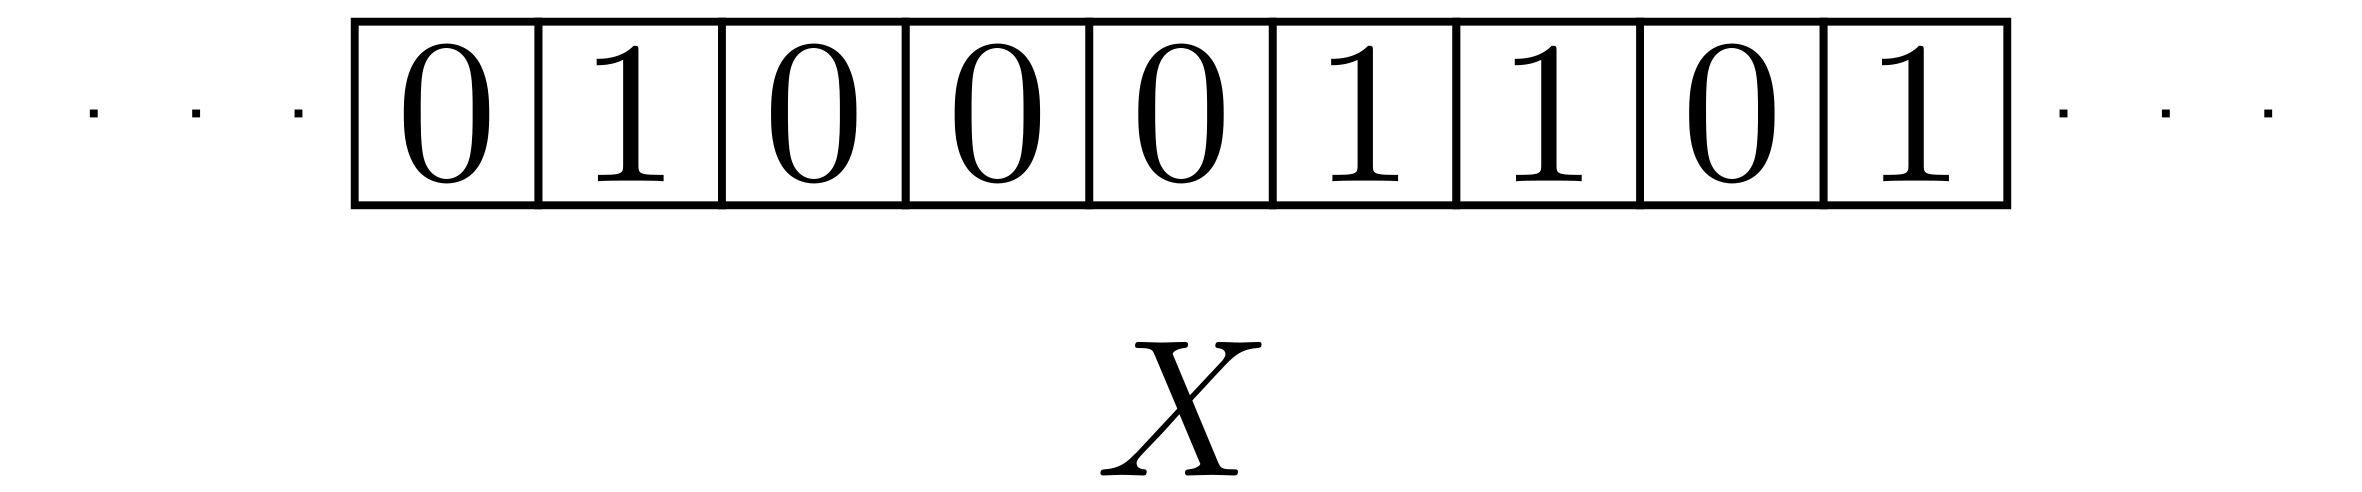
\includegraphics[width=\textwidth]{Figure 6.5.A}
\caption{A Turing machine in state $X$ operates on a single cell at a time}
\end{figure}
\noindent The original conception also required a countably infinite space on the tape.

The instructions necessary to execute $f$ may be stored as a subset of tape $X$ or on a separate tape as if it were an extension of $X$.\footnote{This is the premise of external data storage with a computer program or virus. A computable function should fit on some finite device or a finite space within an infinite device.} As far as the transition function $f$ is concerned, reading and writing is not a one-way process. Rather, it is a mutual form of communication or a dialogue. It is exactly this lack of separation or distinction between a system and its instructions that allows a computer to rewrite itself.

\textbf{Turing completeness}\index{Turing complete} is the ability for a set of rules to imitate a Turing machine $M$. While a Turing machine is an abstraction, it at least has a physical basis in reality. Programming languages are Turing complete without any specific physical limitation or constraints. It is the \textit{rules} that allow it to represent operations on a physical computer or be equivalent to an abstract computer. Programming languages like R or a $\lambda$-calculus like Haskell have different notations, but they are both capable of simulating a Turing machine. What makes as a set of rules Turing complete? How can we prove it is Turing complete?

A \textbf{partial recursive function}\index{general recursive function} or $\mu$-recursive function is a partial function that maps a tuple of natural numbers to a single natural number:
$$f: \mathbb N^k \rightarrow \mathbb N$$
A partial function need only be defined on subsets of the domain $X = \mathbb N^k$. A total function must be defined on the whole domain $X$. A \textbf{total recursive function} produces a defined output for every input.

The set of all total recursive functions with output values in the Boolean set $\mathbb B_\circ = \{0, 1\}$ have complexity class $R$. In other words, a function $f$ of complexity class $R$ has a defined output for some countably infinite Boolean input:
$$f: \mathbb B^{\aleph_0} \rightarrow \mathbb B$$
Computers in the real world depend on the fact that the Cartesian product of a Boolean set can represent a subset of the natural numbers.

We need only show that a rule set may represent partial recursive functions composed of the following primitive recursive functions on the natural numbers:
\begin{enumerate}
\item Constant function $C^k_n$: $C^k_n (x_1,...,x_k) = n$
\item Successor function $S$: $S(x) = x+1$
\item Identity function $P^k_i$: $P^k_i (x_1,...,x_k) = x_i$
\end{enumerate}
We may replace the constant function with the zero function and repeated successor functions such that $C^k_n = S^n (0) = n$. 

We need a few key operators to construct any partial recursive function. We will state that $X = (x_1,...,x_k)$ to simply notation:
\begin{enumerate}
\item Composition operator $\circ$: A function $f$ is composed of $h$ applied to a tuple of functions $(g_1,...,g_m)$ in sequence: 
$$f = h \circ (g_1,...,g_m)$$
such that:
$$f(X) = h \big ( g_1(X),...,g_m(X) \big )$$ 
Let functions $g$ and $h$ be defined as:
$$g(x_1,...,x_k); \ h(x_1,...,x_m)$$
meaning that $g$ operates on a $k$-tuple of natural numbers and $h$ operates on an $m$-tuple of natural numbers.
\item Primitive recursion operator $\rho$: $\rho(g, h) = f$ in which the initial memory function $f(0, X)$ is equal to $g$:
$$f(0, X) = g(X)$$ 
and a new value is determined by applying the function $h$ according to the previous iteration of the recursive memory function $f(i, X)$:
$$f(i+1, X) = h(i, f(i, X), X)$$ 
for a total of $n$ iterations, $i \in \{0,...,n-1\}$.
\item Minimization operator $\mu$: The minimum value of a function $f$ is given by the first time it returns $0$:
$$ \mu (f)(X) = j \iff f(j, X) = 0 \ \textnormal{and} \ f(i, X) > 0$$
for all $i \in \{0,...,j-1\}$. Recall that $0$ is the minimum value of the natural numbers.
\end{enumerate}
Suppose the primitive recursion $\rho$ continues infinitely without constraint. If the minimization operator successfully finds the minimum value, it returns the first value $j$ that successfully does so. The problem is that if there is no value for which $f(i, X)$ that is equal to $0$, then the minimization operator $\mu$ will never halt and return some value $j$ because the minimizing value does not exist.\footnote{A simple example of a function that cannot be minimized is if its recursion becomes trapped in a cycle of values such as $(1, 4, 2, 1, 4, 2, 1 . . .)$.}

Any partial recursive function operating on a finite linear tape $X$ of length $N$ may be considered to be representing a subset of the natural numbers $S \subset \mathbb N$, \ $|S| = |A|^N$. For example, a Boolean alphabet can represent $2^N$ natural numbers such as the subset $S = \{0, 1, 2,...,2^N-1\}$. This is essentially how an $N$-bit operating system computer stores blocks of memory:
$$S = \begin{bmatrix} s_1 & s_2 & s_3 & s_4 & s_5 & s_6 & s_7 & s_8 \\
s_{9} & s_{10} & s_{11} & s_{12} & s_{13} & s_{14} & s_{15} & s_{16} \\
s_{17} & s_{18} & s_{19} & s_{20} & s_{21} & s_{22} & s_{23} & s_{24} \\
s_{25} & s_{26} & s_{27} & s_{28} & s_{29} & s_{30} & s_{31} & s_{32} \\
s_{33} & s_{34} & s_{35} & s_{36} & s_{37} & s_{38} & s_{39} & s_{40} \\
s_{41} & s_{42} & s_{43} & s_{44} & s_{45} & s_{46} & s_{47} & s_{48} \\
s_{48} & s_{50} & s_{51} & s_{52} & s_{53} & s_{54} & s_{55} & s_{56} \\
s_{57} & s_{58} & s_{59} & s_{60} & s_{61} & s_{62} & s_{63} & s_{64}
\end{bmatrix}$$

\noindent The above matrix is an abstract representation of a block of memory with $64$ bits, and it may uniquely represent any element from the set $S = \{0, 1, 2,...,2^{64}-1\}$. For a relatively simple transition function $f$, this memory block $S$ with a finite countable set of states could be used to augment the behavior of the transition function $f$.\footnote{This augmentation is what we meant by a finite space to write an algorithm, defining a computable function.}

Let us define an example where the tape $X$ is separate from some memory block $S$ that stores data about how some primitive transition function $f$ will operate next. A read action on a transition function could be interpreted as some Boolean mapping $r: X \rightarrow S$ and a write action as some Boolean mapping $w: S \rightarrow X$. Therefore, the tape $X$ can read how to rewrite itself using external instructions $S$. This abstraction of a read-write cycle governs how classical computers work in current times.

A $64$-bit program written on $S$ with a primitive transition function $f$ has enough memory to write infinitely on a two-dimensional tape $X$. For example, we may compute the binary representation of a Fibonacci number:
\begin{figure}[H]
\centering
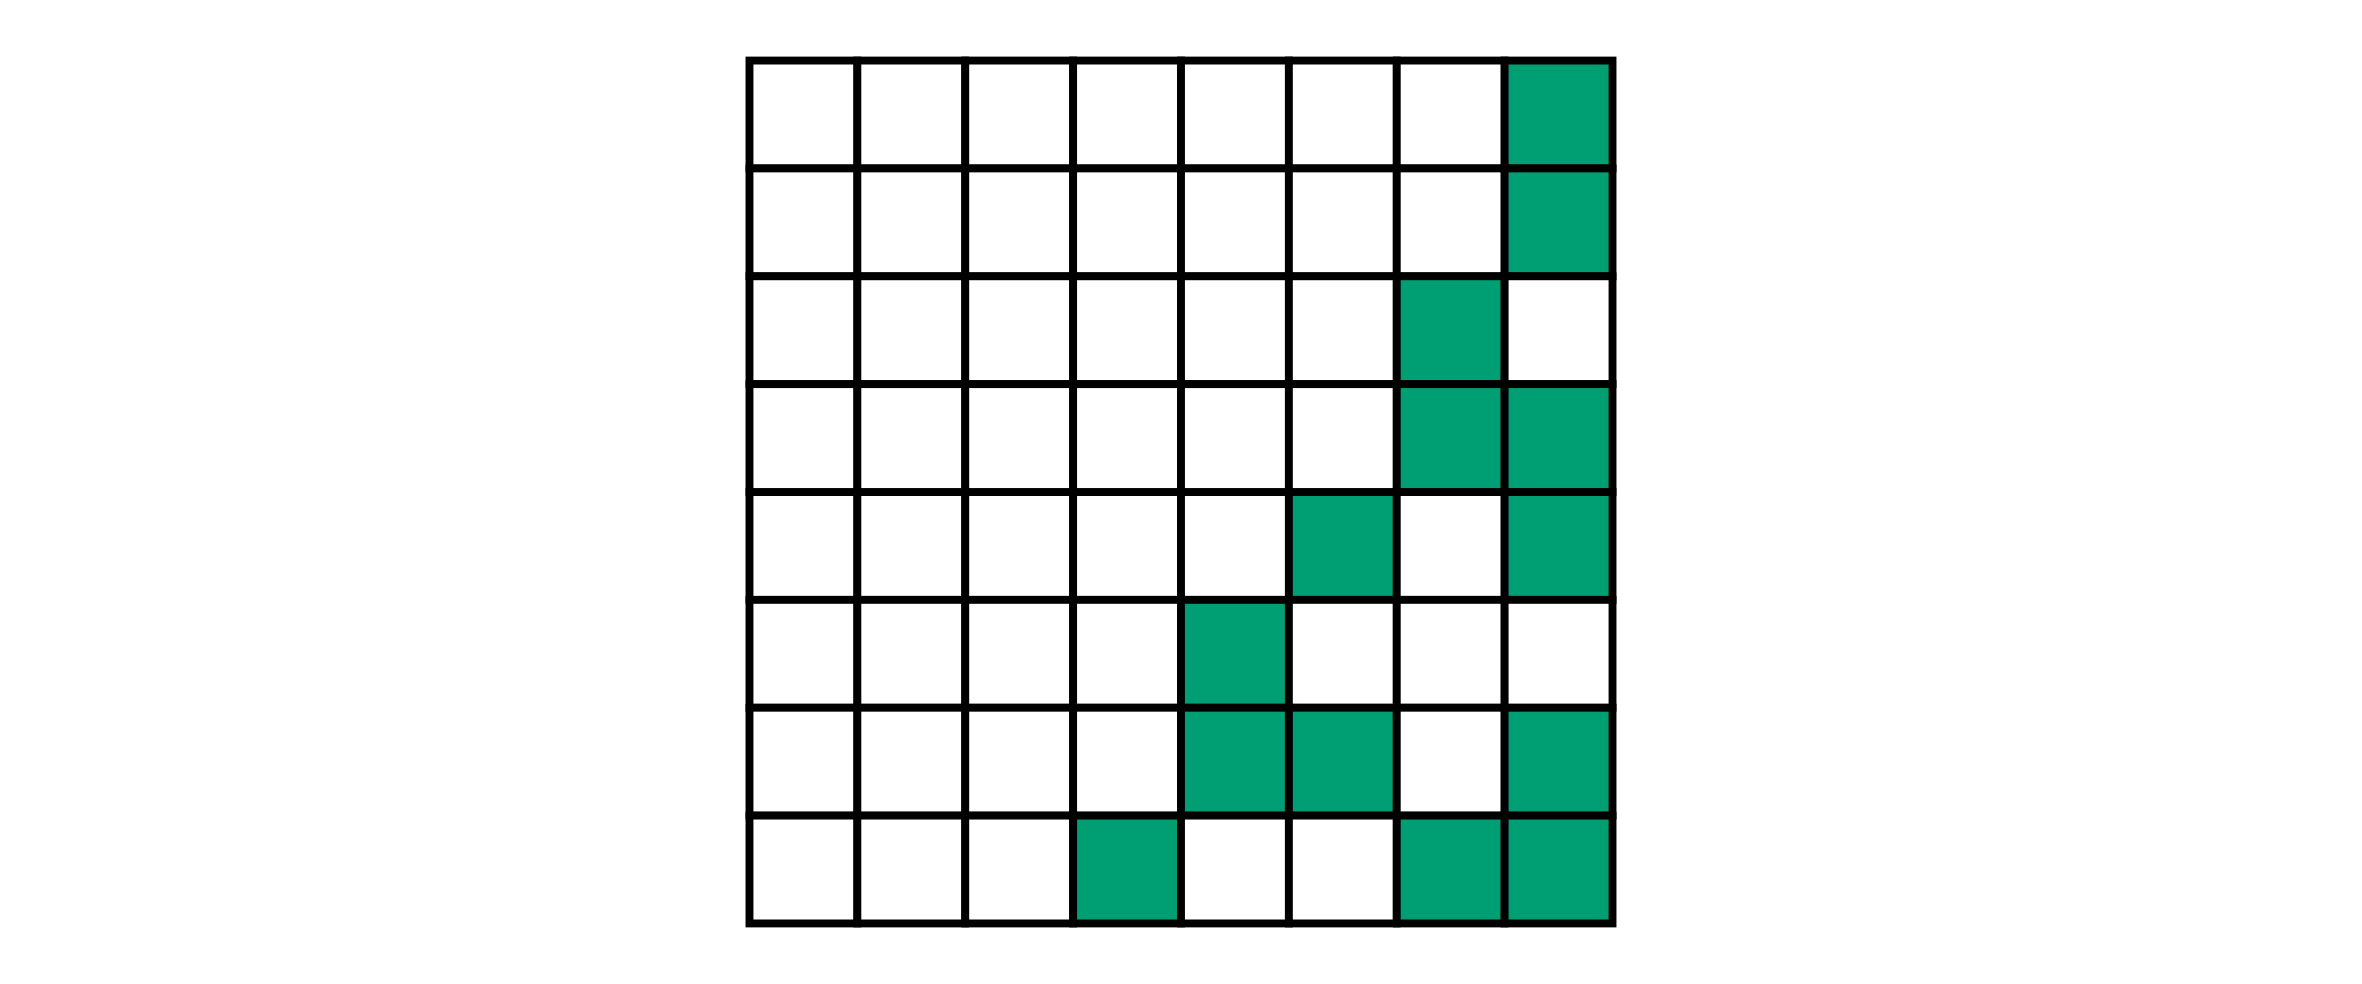
\includegraphics[width=\textwidth]{Figure 6.5.B}
\caption{The Fibonacci sequence in binary on a 2D Turing machine}
\end{figure}
\noindent by reading and writing upon one cell at a time. Is there a limit to the largest Fibonacci number that may be computed with a $64$-bit program $S$?


\section{Probabilistic Turing Machines}

A \textbf{probabilistic Turing machine}\index{probabilistic Turing machine} is a Turing machine with a transition function that may result in a random evaluation for any given input. Otherwise, it has many of the same properties as a deterministic Turing machine. A probabilistic Turing machine is a type or subset of a non-deterministic Turing machine. While a non-deterministic Turing machine may explore all possible branching paths each time there is a random transition function, a probabilistic Turing machine may only walk one specific realized path at a time.
\begin{figure}[H]
\centering
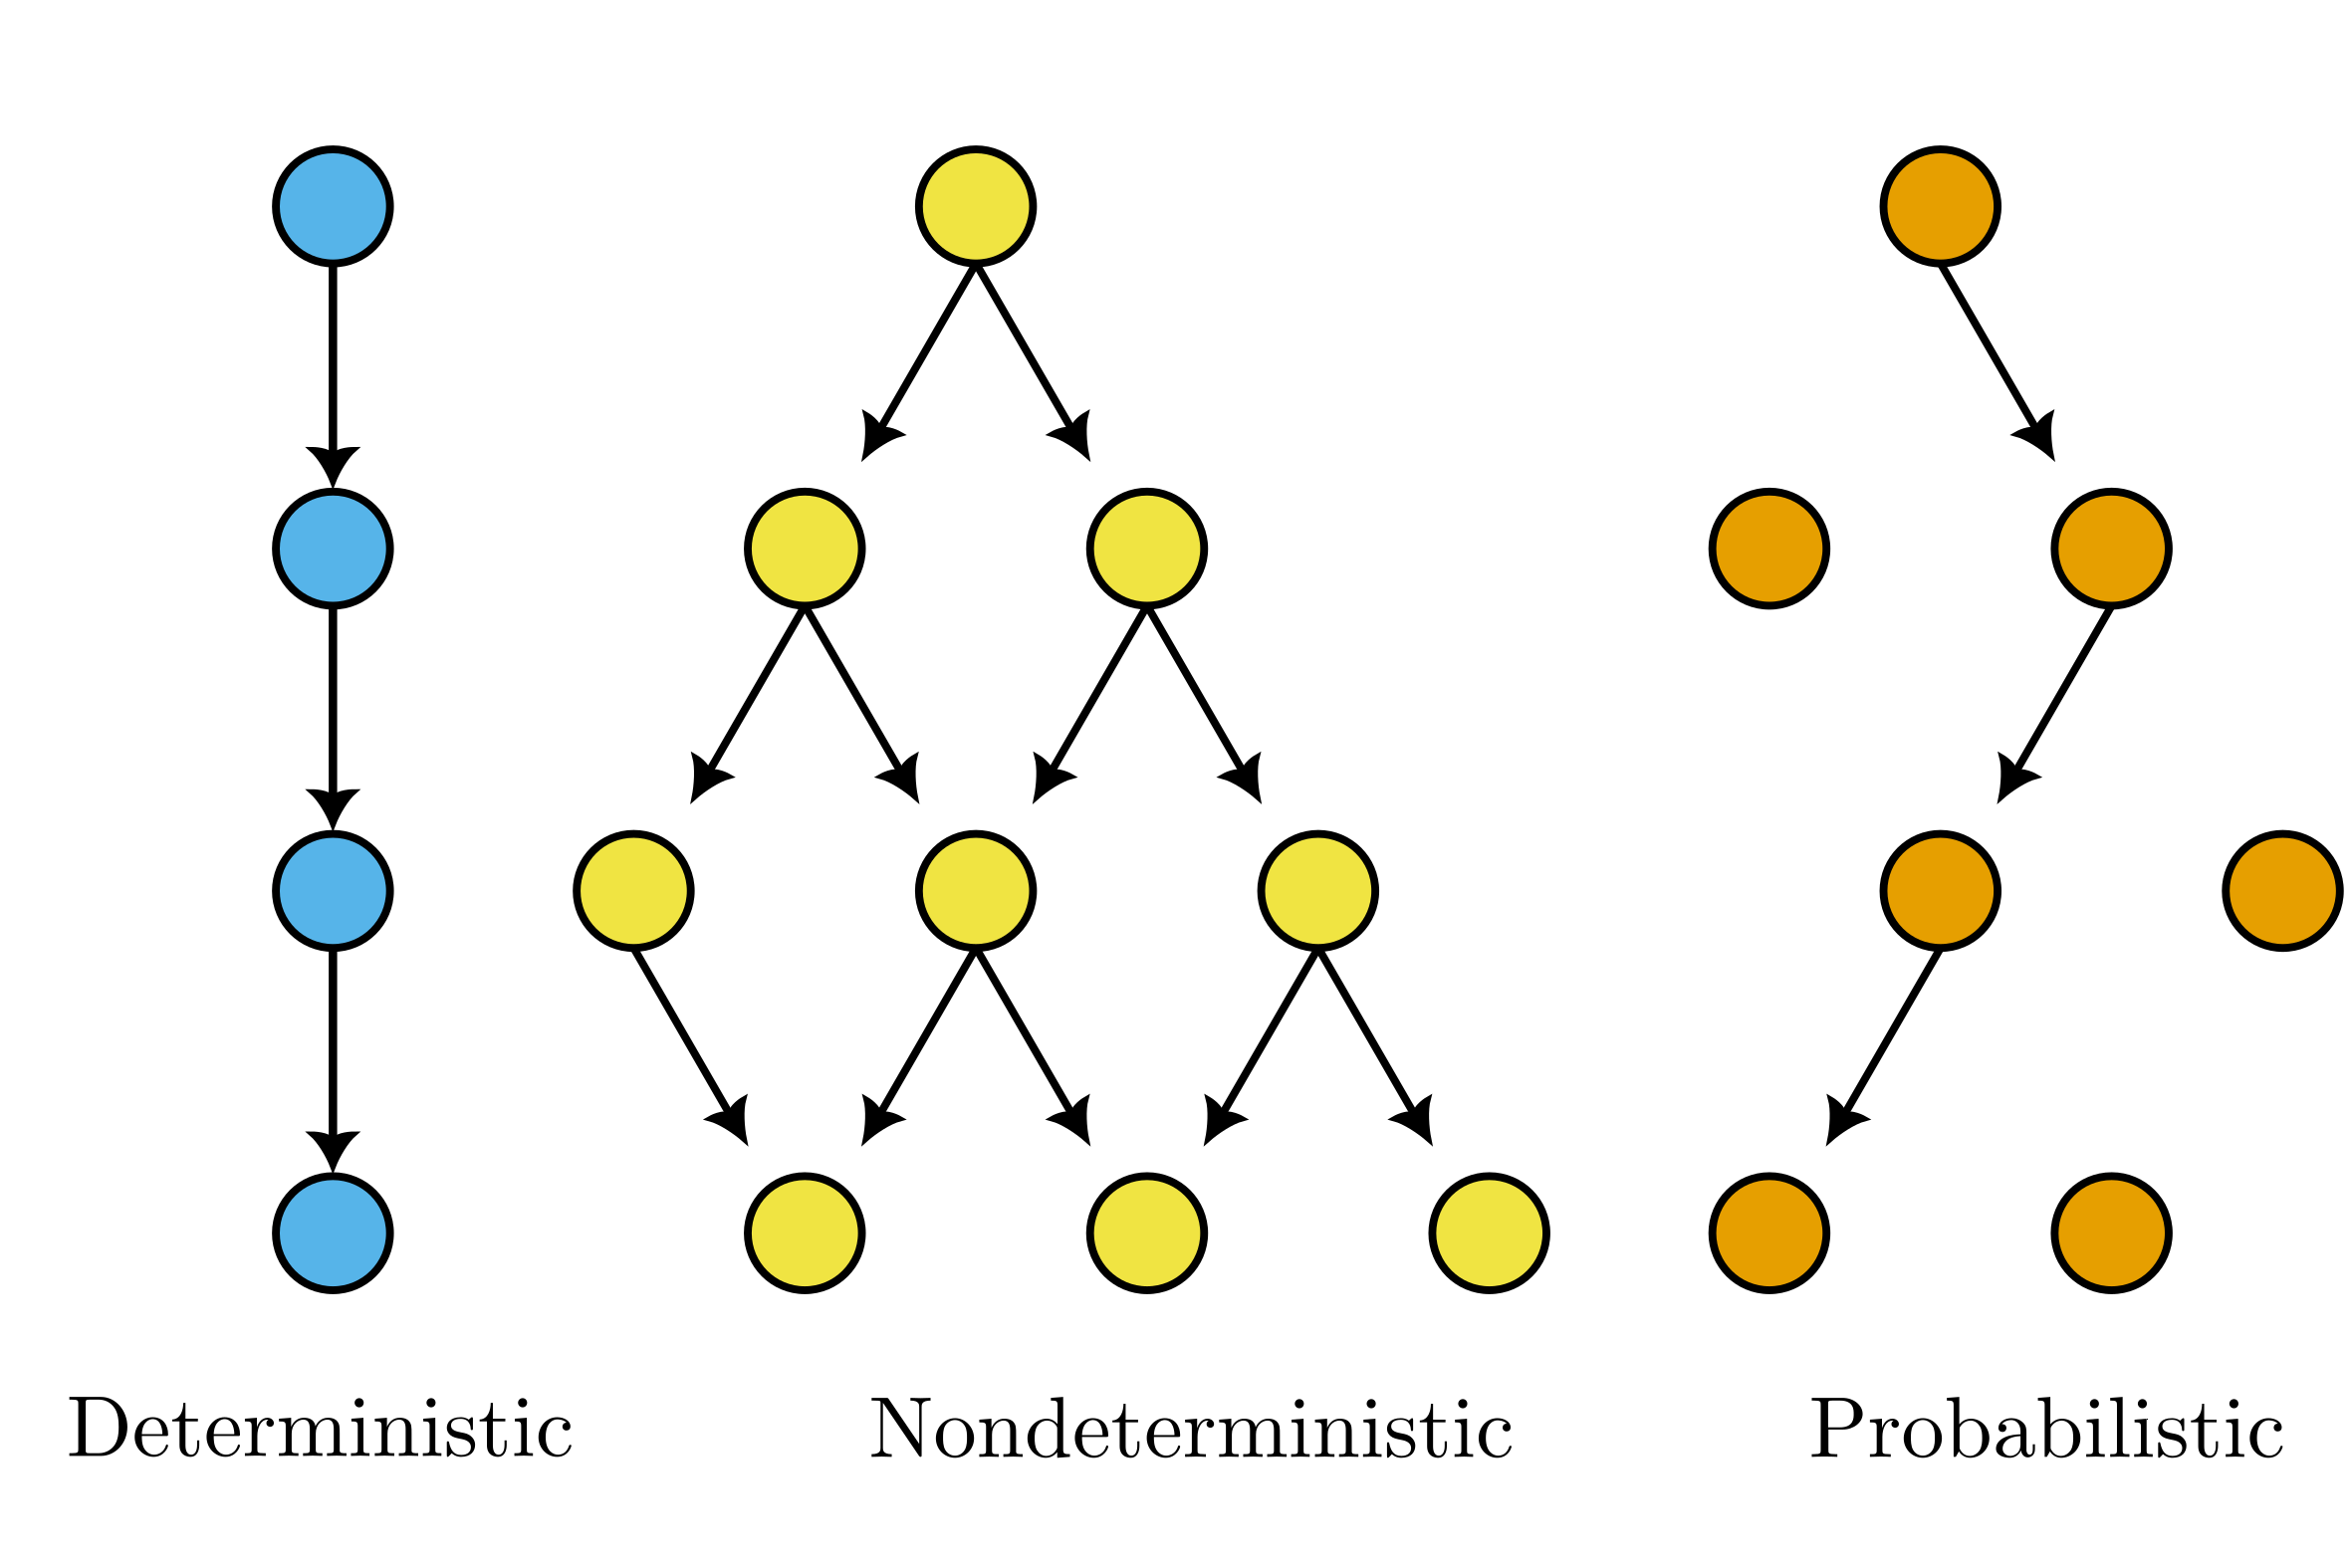
\includegraphics[width=\textwidth]{Figure 6.6.A}
\caption{A probabilistic Turing machine may only experience one path}
\end{figure}
This leads into the problematic philosophy of counterfactual definiteness, or inference via absence. For finite games like Battleship puzzles, inference via absence is appropriate. For real-life hide and seek, the hider may simply lie to the seeker about being in a finite space.

Considering the transition function $f$, the probability measure $\mu$, and the pushforward measure $\Lambda_\sharp \mu$. The system is determined to be in an initial state $X_0$ with probability 1. The following relationship:
$$ \Lambda_\sharp^t \mu(f^t (X_0)) = \mu(X_0) = 1$$
states that the $t$-th pushforward measure upon the $t$-th transition function iteration of $X_0$ obeys the law of total probability for a total mass of $1$. The transition function is deterministic if and only the pushforward measure of any state has entropy $0$:
$$ -\mathrm{E}[\mu(X_0) \cdot \ln(\Lambda_{\sharp} \mu(X_0))] = 0$$
for any initial state $X_0 \in \mathcal X$ for all possible future time step $t \in \mathbb N$. Else, the transition function is stochastic for at least one state.

A probabilistic Turing machine $M$ is a tuple that consists of the following:
\begin{quote}
$A$: the alphabet, including the blank symbol $0$ or $\varnothing$

$X_0$: the initial system state at time $t=0$ of size $N$ symbols

$\mathcal X$: the set of all permutations of $X$ using the alphabet $A$, $X \in \mathcal{X} = \prod\limits_{i=1}^N A$

$F$: a subset of $\mathcal{X}$ denoting the final states that the transition function will halt at

$f$: the stochastic transition function in which $f(X_t) = X_{t+1}$, and it realizes one random choice among shifting the tape $X$ left, right, or overwriting a symbol
\end{quote}
The rules of a probabilistic Turing machine differ little from a deterministic Turing machine. Real-life computers are idealized as deterministic, but the outcomes of the motion of electrons themselves are inherently probabilistic and subject to random environmental influences.

Suppose that a 3D Boolean random walk system $X_t$ has a subset $S_t$ that represents a linear tape, and $S_0$ is the initialized tape. We call $X_t / S_t = Y_t$ to refer to the system without the tape (the program):
\begin{figure}[H]
\centering
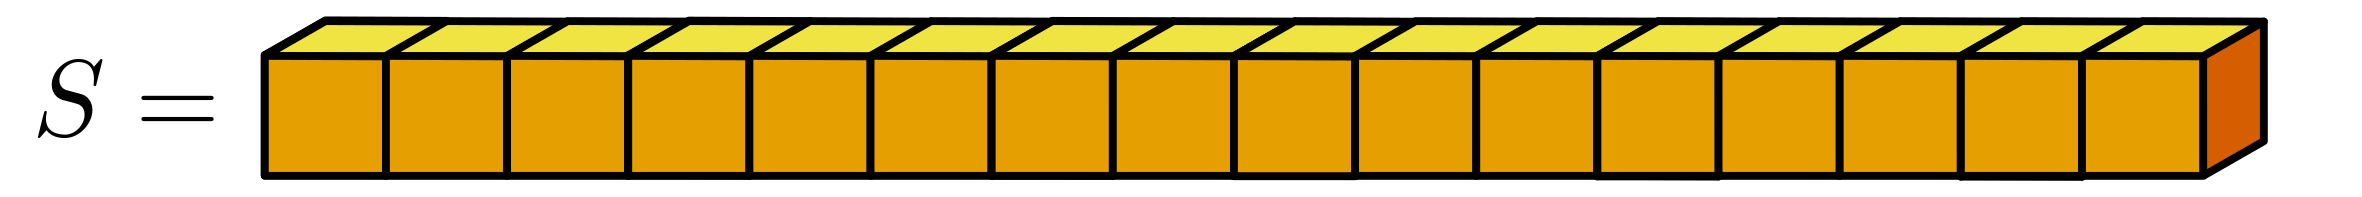
\includegraphics[width=\textwidth]{Figure 6.6.B}
\caption{A linear subset of a 3D Boolean random walk is $S_t$}
\end{figure}
\noindent
For sufficiently large $Y$, it is possible to program almost any distribution on the future linear tape $S_1$ as if $Y$ was a mapping function, $Y: S_0 \rightarrow S_1$. This works because a Boolean random walk's transition function is not spatiotemporally local, thus distant cells have some influence on the outcome of $S_1$. We may more easily construct some arbitrary distribution on futures $S_2$, $S_3$, or higher.

We may also more easily construct some arbitrary distribution if we choose a smaller space for $S$ due to needing to control less entropy. Imposing arbitrary distributions on finite spaces is a direct result of Shannon's \textbf{noisy-channel coding theorem}\index{noisy-channel coding theorem}, stating that it is possible to send a signal transmission rate $R$ through a noisy channel with capacity $C$ with arbitrarily low error if $R < C$. This value $C$ is known as the \textbf{Shannon's limit}\index{Shannon's limit} of the channel. If the source entropy rate $R$ is higher than that Shannon's limit entropy rate $C$, it is certain the signal experiences information loss at a rate of $R-C$. Even if there is noise in the channel, any signal beneath Shannon's limit can be encrypted via some error-correcting code to be lossless. The trick is to \textit{use the noise} in the channel to \textit{protect the signal}.

It is a lot easier to achieve an exact distribution on $S_t$ if we have no restrictions on the shape of $S$ or how much time it will take to achieve it.\footnote{At the extreme case, we remove the requirement that cells in $S$ are contiguous.} Finding some exact environment $Y_0$ upon $S_0$ of arbitrary shape to get a specific distribution for $S_t$ is computationally impractical, even though it seems to happen quite often in real-life processes. For example, the atomic bonds of a molecule may be considered an encryption-decryption process that is affected by environmental programs such as catalysts, inhibitors, or catalyst poisons.\footnote{A catalyst poison decrypts a catalyst, rendering it inert.} Viruses breach the carefully crafted security of a cell's firewalls using programs made of organic chemistry, using the power of random evolution to defeat the finite game.

While any computable function is possible, the necessary preconditions must occur for the transition function to chain into that state. This is true of Boolean random walks just as well as whatever true digital physics theory would underlie reality. A digital physics theory of everything would need to preclude local realness. Boolean random walks denies strictly local interactions via checker chains in order to allow a real-valued probability for each element of the state space. Boolean statistical mechanics decides upon denying locality but allowing realness, also known as the assumption that an unknown state was actually definitely a specific state with probability $1$. This is the fundamental to the definition of a \textbf{probabilistic Turing machine}: it was definitely in one state in the past and it took a specific sequence to get from state $X_0$ to state $X_t$.

It is worth recalling that our definition of a stochastic transition function $f(X_t) = X_{t+1}$ means that we may recursively define the following:
$$X_t = \underbrace{f \circ f \circ ... \circ f}_{t \ \textnormal{times}} \circ X_0$$
If we combine this notation with the notation for differential equations:
$$\frac{d}{dt}f(t) = Q f(t)$$
then we can explicitly state that:
$$Q = \frac{f'(t)}{f(t)} = \frac{d}{dt}\ln (f(t))$$
such that we may rewrite our time equation as an exponential equation:
$$e^{Q} = f(t)^{\frac{d}{dt}}$$
With a little abuse of notation, we may write:
$$e^{\int Q dt} = f(t)^{\int\frac{d}{dt}dt} $$
$$e^{Q t} = f(t)$$
We see that $Q$ is the logarithm of some function pushforward. We should be more specific in stating that there is an implied identity function or identity matrix $I$. This $I$ is the definition of $f(0)$ since:
$$f(0) = e^{Q \cdot 0} = I$$

In the later chapters such as \textit{\S 9 Boolean Mechanical Systems}, we will prefer restrict $Q$ to be the matrix logarithm of the (right) stochastic transition matrix $P$. In our preferred column eigenvector notation, we may state $X_0 e^{tQ}$ = $X_t$ or refer to our pushforward measure definition:
$$\mu_0(X_0) = \mu_0(\Lambda^{-t}X_t)$$
to define stochastic eigensystems of $X$. We will describe more about eigenvalues during \textit{\S 7.5 Transition Matrix} and differential equations in \textit{8.2 Ordinary Differential Equations}.

\section{Stochastic Turing Systems}
A \textbf{stochastic Turing system}\index{stochastic Turing system} (STS) is an infinite time and infinite space probabilistic Turing machine that has, that will, and is executing every possible decision problem of complexity class $R$. It therefore executes every computable function a countably infinite amount of times per finite time step. Furthermore, it is executing every possible permutation of an algorithm and tracing every possible route through a finite set of states. Note that this means any state is possible, but not \textit{every finite route between states} is possible. Impossible paths represent impossible computations or illogical sequences. In fact, every finite route between states is possible if and only if every state can reach any other state in a single time step.

The Church-Turing thesis states that a function can only be computed in finite time with a deterministic algorithm if it may be computed on a deterministic Turing machine. If you assume that the \textit{Church-Turing thesis} applies to our physical reality, then it is relatively safe to assume that our universe must obey the laws of a stochastic Turing system. This of course does not constitute a proof. Our specific \textit{chronos chroma cosmos}, or time-color space, may not behave precisely like a Boolean mechanical system governed by a Boolean random walk. However, our universe may simulate a Boolean random walk or likewise be simulated by a Boolean random walk. If you assume our universe is infinite in time and space and that it may manufacture finite almost-deterministic Turing machines, then is it necessarily governed by computable functions? What would it mean to have a reality that does not obey the laws of computable functions? 

Suppose that a Boolean random walk of infinite space on a 3D lattice $\mathbb Z^3$ is initialized using the Bernoulli distribution using the Boolean set $\mathbb B_\pm = \{-1, +1\}$ and probabilities $p = 1-p = \frac{1}{2}$. A subsystem of the infinite Boolean mechanical system is labeled $X$, and it is a fixed space of connected cells forming a rectangular prism.
\begin{figure}[H]
\centering
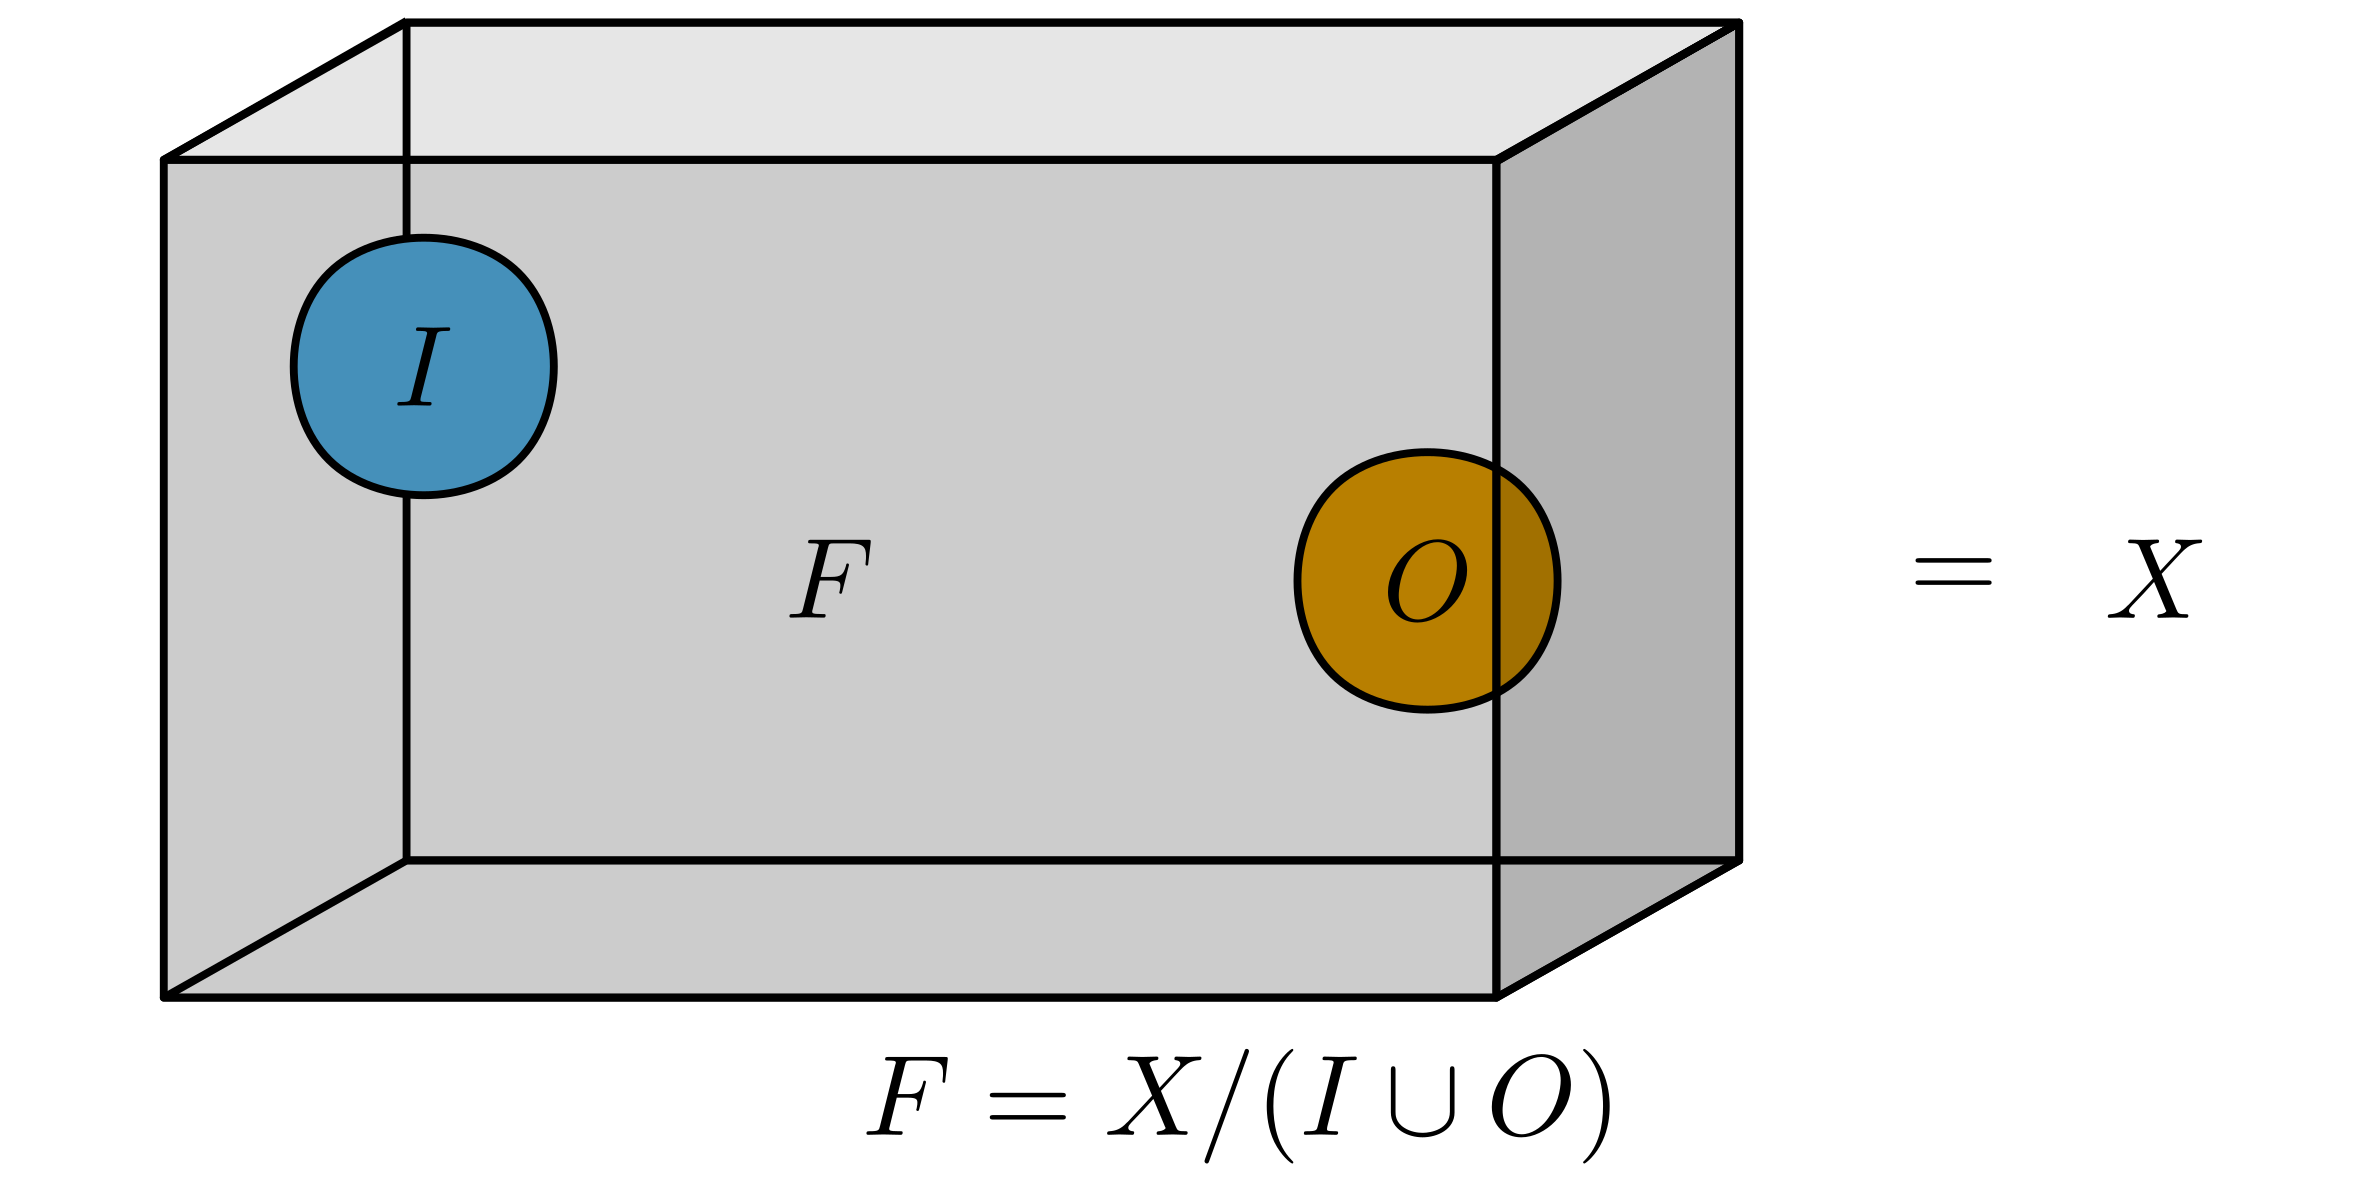
\includegraphics[width=\textwidth]{Figure 6.7.A}
\caption{There exists some region $F$ in which input $I$ gives some output $O$ for small $I, O$}
\end{figure}
We may attempt to emulate the deterministic Boolean function $f: \mathbb B^n \rightarrow \mathbb B^m$ using the input region $I$ and output region $O$ with cardinalities $|I|\geq n$, $|O| \geq m$ using the region $F$ in which $f(x)$ is approximated using input $I_0$ and output $O_t$ for $t \geq 1$. In fact, the infinite lattice $Z^3$ that is randomly initialized has infinite copies of any particular subsystem $X$. As $t \rightarrow \infty$, the algorithm contained in $X$ of cardinality $|X|=N$ reaches its asymptotic distribution in space. If we know the natural noise distribution of space, then we can protect any signal that is beneath Shannon's limit via error-correcting codes or even co-opt the noise in the protection of the signal.

The input space $I$ and the output space $O$ need not be contiguously connected set of cells. In fact, it is more ideal for our ability to construct any algorithm with input $I_0$ and output $O_t$ if we loosen the restriction on the exact positions of $F$, $I$, and $O$ within the system $X$. If we do require that $I$ is connected and $O$ is connected, then algorithm space $F$ may require an indeterminate amount of space or indeterminate length of time to represent a specific algorithm. There can be no general algorithm to determine if there exists some indeterminate $F_0$ upon fixed $I_0$ that produces a desired output upon $O_t$, and likewise there can be no general algorithm to determine if there exists some indeterminate $I_0$ upon fixed $F_0$ that produces a desired output upon $O_t$. That would solve the \textbf{halting problem}\index{halting problem}. The halting problem states that there is no general algorithm to determine if a program will halt upon a set of target states within a finite amount of time.

Recall that any signal in a noisy channel can be made lossless in a noisy channel. Since we have may guarantee the creation of almost-lossless information packets in Boolean random walks, we can guarantee the ability to emulate any deterministic Boolean function at a macroscopic scale. At this macroscopic scale, we may write detailed programs with almost-deterministic Turing machines. Due to the determinism, no algorithm may determine if any other program will make produce a target state within a finite time with near-certain probability $1-\varepsilon$. Due to the randomness, we as gods can guarantee that an infinite amount of time is enough to produce the target state with probability $1$. We just might starve before we get to see it happen.

In 1947, Andrey Markov Jr. showed that the \textbf{word problem}\index{word problem} for semigroups is undecidable.\footnote{Andrey Markov Jr. is the son of Andrey Markov, for which the Markov chain is eponymously named.} The word problem asks if any two logical expressions $X$ and $Y$, using languages $\Lambda_X$ and $\Lambda_Y$, are equal with respect to some \textit{rewriting identities}, such as $\neg A \cup \neg B = \neg (A \cap B)$. However, there are infinitely many equivalent ways to write any particular algorithm in a Turing complete system. This means there is no general algorithm to determine any two Boolean mechanical systems $X$ and $Y$, each operating under a unique transition function $f_X$ and $f_Y$, encode the same algorithm. Such an algorithm would solve the halting problem, which is undecidable. This means that it is also impossible for two subspaces of a Boolean mechanical system to use a general algorithm to determine if they are ``allies'', and that means that there is no such that as a faultless pure infection algorithm.

A \textbf{pure infection algorithm}\index{pure infection algorithm} is a finite algorithm $X$ in space that is capable of classifying another finite algorithm $Y$ in space, then overwrite it with a copy of itself. It attempts to translate the instructions written on $Y$ into its own language. It will ignore $Y$ if it is a clone or ally, kill $Y$ if it is not a clone or ally, and infect $Y$ if it is available. However, $A$ cannot possibly hope to classify infinitely many algorithms upon $Y$ of differing sizes. That would solve the word problem, which is undecidable.\footnote{This is also known as the grey goo catastrophe, in which nanomachines consume a planet until it is nanomachines. Such runaway technology is impossible because it is paramount to solving the halting problem.}

Consider the Collatz conjecture with a function $f$ and input $x \in \mathbb N$:
\[
f(x)
\begin{cases}
x/2, & \textnormal{if} \ (x \ \textnormal{mod} \ 2) = 0\\
3x+1, & \textnormal{if} \ (x \ \textnormal{mod} \ 2) = 1
\end{cases}
\]The \textbf{Collatz conjecture}\index{Collatz conjecture} asks if a composition of $f$ upon $x$ eventually results with an output 1. Formally, we wish to know if this statement is true:
$$\exists n \in \mathbb N: f^{(n)} (x) = 1, \quad \forall x$$
It is a sort of rewriting rule or language translation rule. Any attempt to determine if the inverse function $f^{-1}$ covers all natural numbers $\mathbb N$ is undecidable. If a Collatz conjecture solution exists, it cannot be solved this way.

A little philosophy before we continue deeper. A true Boolean mechanical system has no clear distinction between observer and observed, operator and operand, etc. If the complete infinite future of any 3D stochastic Turing system is undecidable, then concepts like verification, trust, deception, and betrayal are deeply fundamental to how the universe works. Labels cannot be ascertained \textit{a priori} and must play out first. In a way the limits of a 3D stochastic Turing system tell us what we already know and fear: that the universe is inherently chaotic with limited predictability. That we may not merely observe an object and predict its infinite future as friend or foe. Oh, what mortal men would give to know every path to some desired outcome without taking it one step at a time!

\begin{figure}[H]
\centering
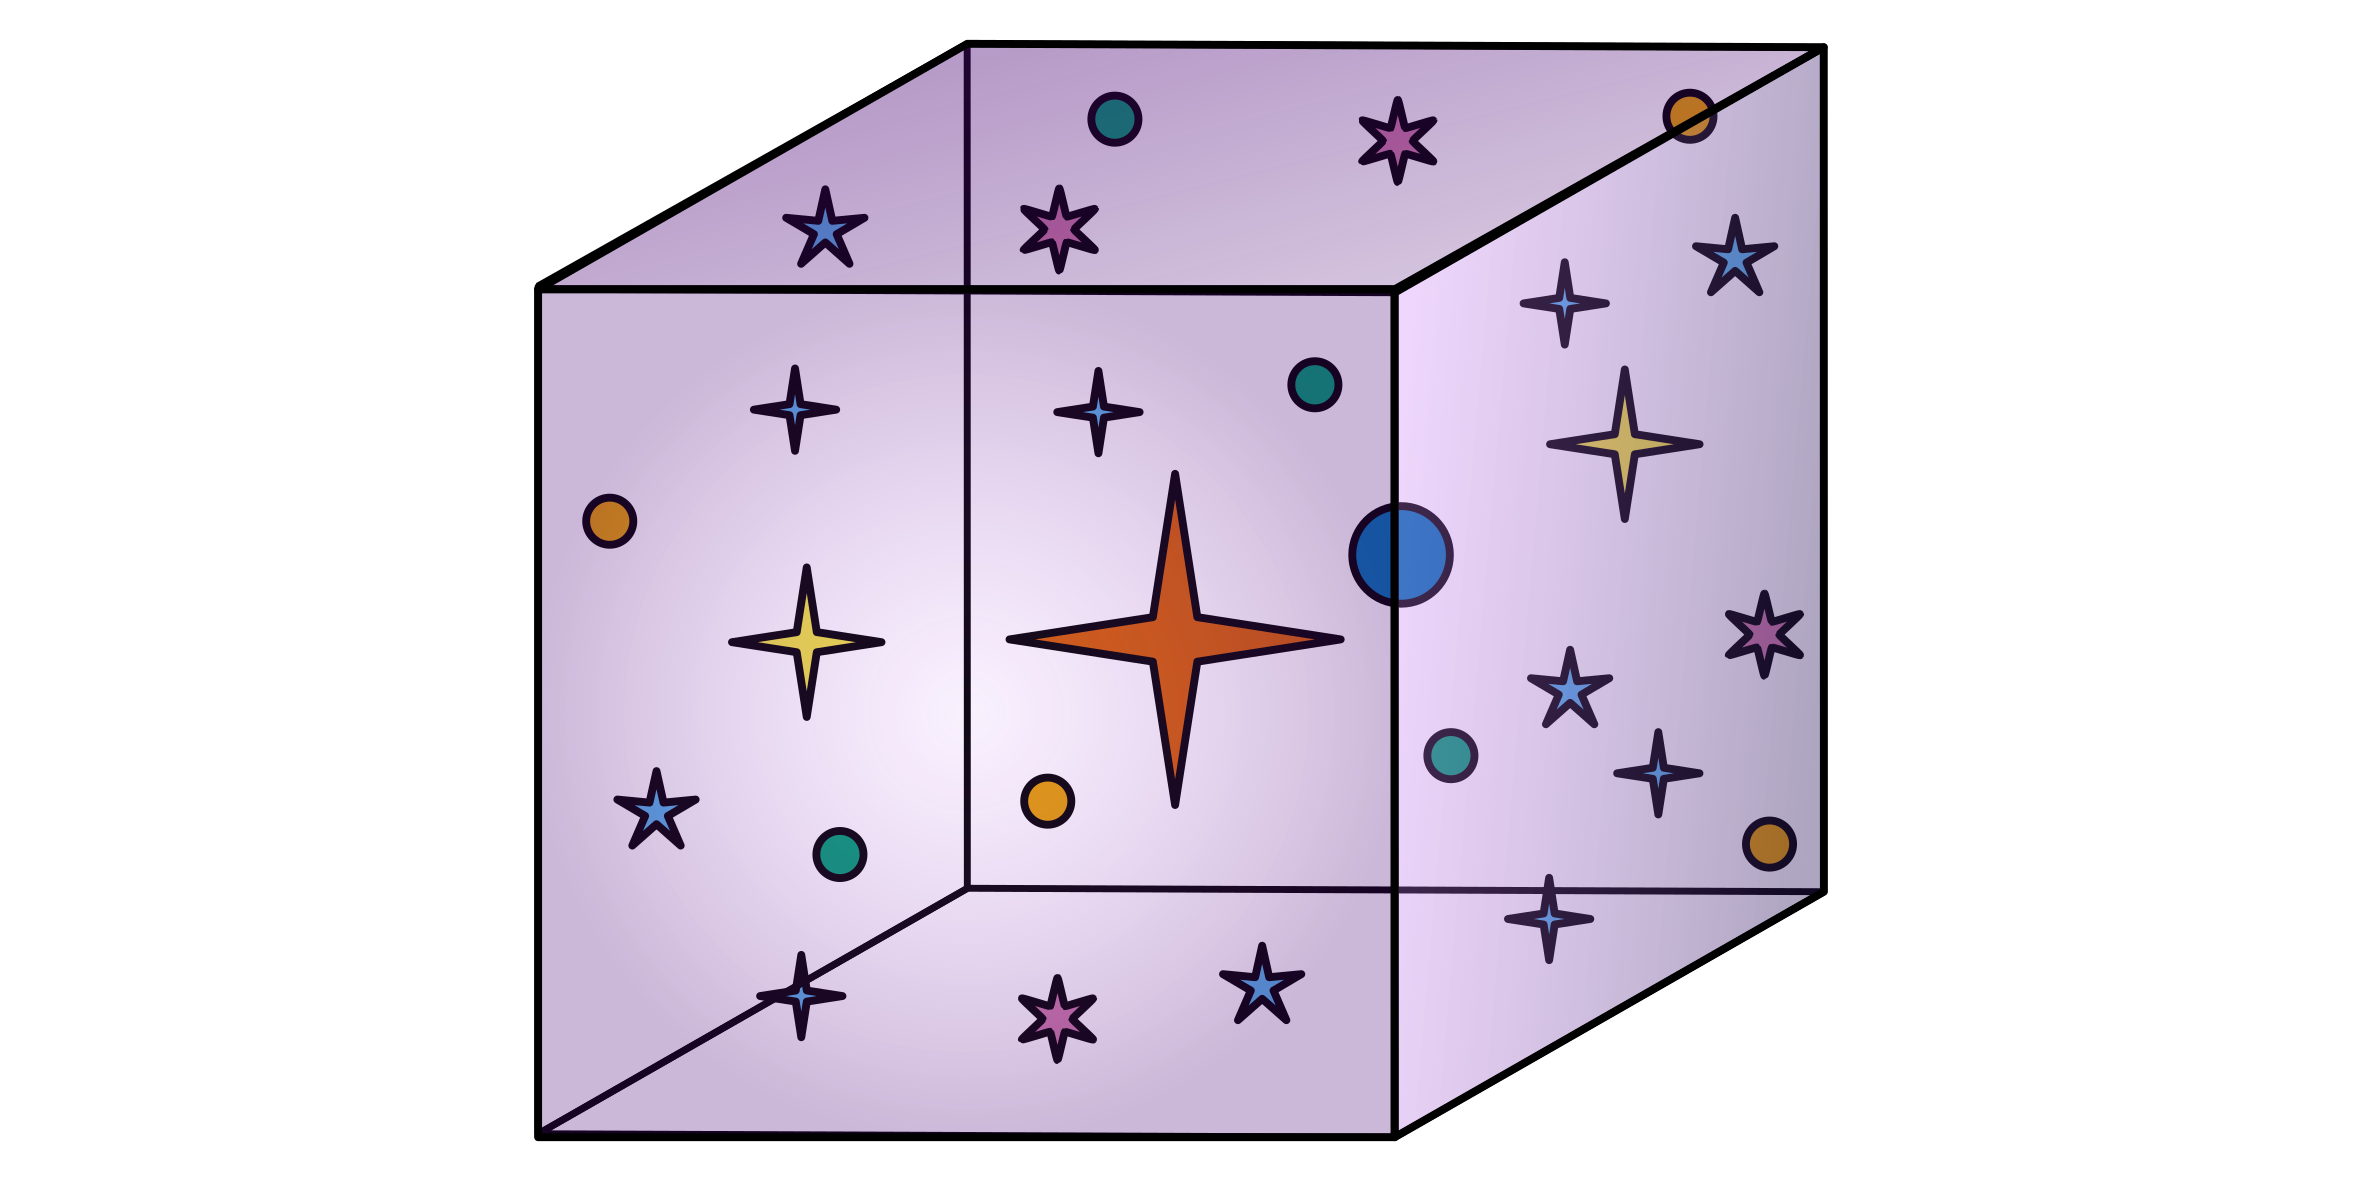
\includegraphics[width=\textwidth]{Figure 6.7.B}
\caption{The machine within the black box}
\end{figure}


We pitiful mortals can only ever see the input, the output, and the surface of the black box. yet even if we were to peer inside and view the exact machinations inside, we would fail to completely comprehend its unlimited future and translate it by human means. When we see its future for the first time, it will already be present for the last time, and then the past forever. We never see the unexplored futures, only the singularity of the now, that what could have been has collapsed to. What we desire to know for certain is that which is most out of reach, the unpredictable future.

\section{Computational Complexity}
\textbf{Computational complexity}\index{computational complexity} refers to the amount of resources that must be allocated to run an algorithm or solve a problem. These resources may be time or space, although a more appropriate term for space is either memory or capacity. Since I assert Boolean mechanics as a candidate theory of time and space in our universe, it is important to address computational complexity classes such as $\textbf{P}$, $\textbf{NP}$, $\textbf{RP}$, $\textbf{BPP}$, and $\textbf{PP}$. All these problems in these classes are implicitly of complexity class $R$, or solvable on a computer. One of the Millennium Prize Problems is to prove or disprove whether \textbf{P} $=$ \textbf{NP}.

A $\textbf{BPP}$ algorithm produces the correct answer or solution to a computation problem with probability $p$ in which $(2/3 \leq p < 1)$. We are interested in the class $\textbf{BPP}_\textnormal{path}$ since it is a superset of \textbf{NP} and we allow our computation paths to be of variable length. This is similar to what we consider the existence of an algorithm in a Boolean mechanical system. 

Consider multiple parallel runs of a Boolean mechanics simulation that imitate the fusion of two hydrogen atoms (deuterium and tritium) into one helium atom and a neutron. Consider a set of random initial states $\hat I_1,...,\hat I_n$ within input space $I$ near a that may randomly transition into some target states $\hat O_1,...,\hat O_m$ on output space $O$ in the future:
\begin{figure}[H]
\centering
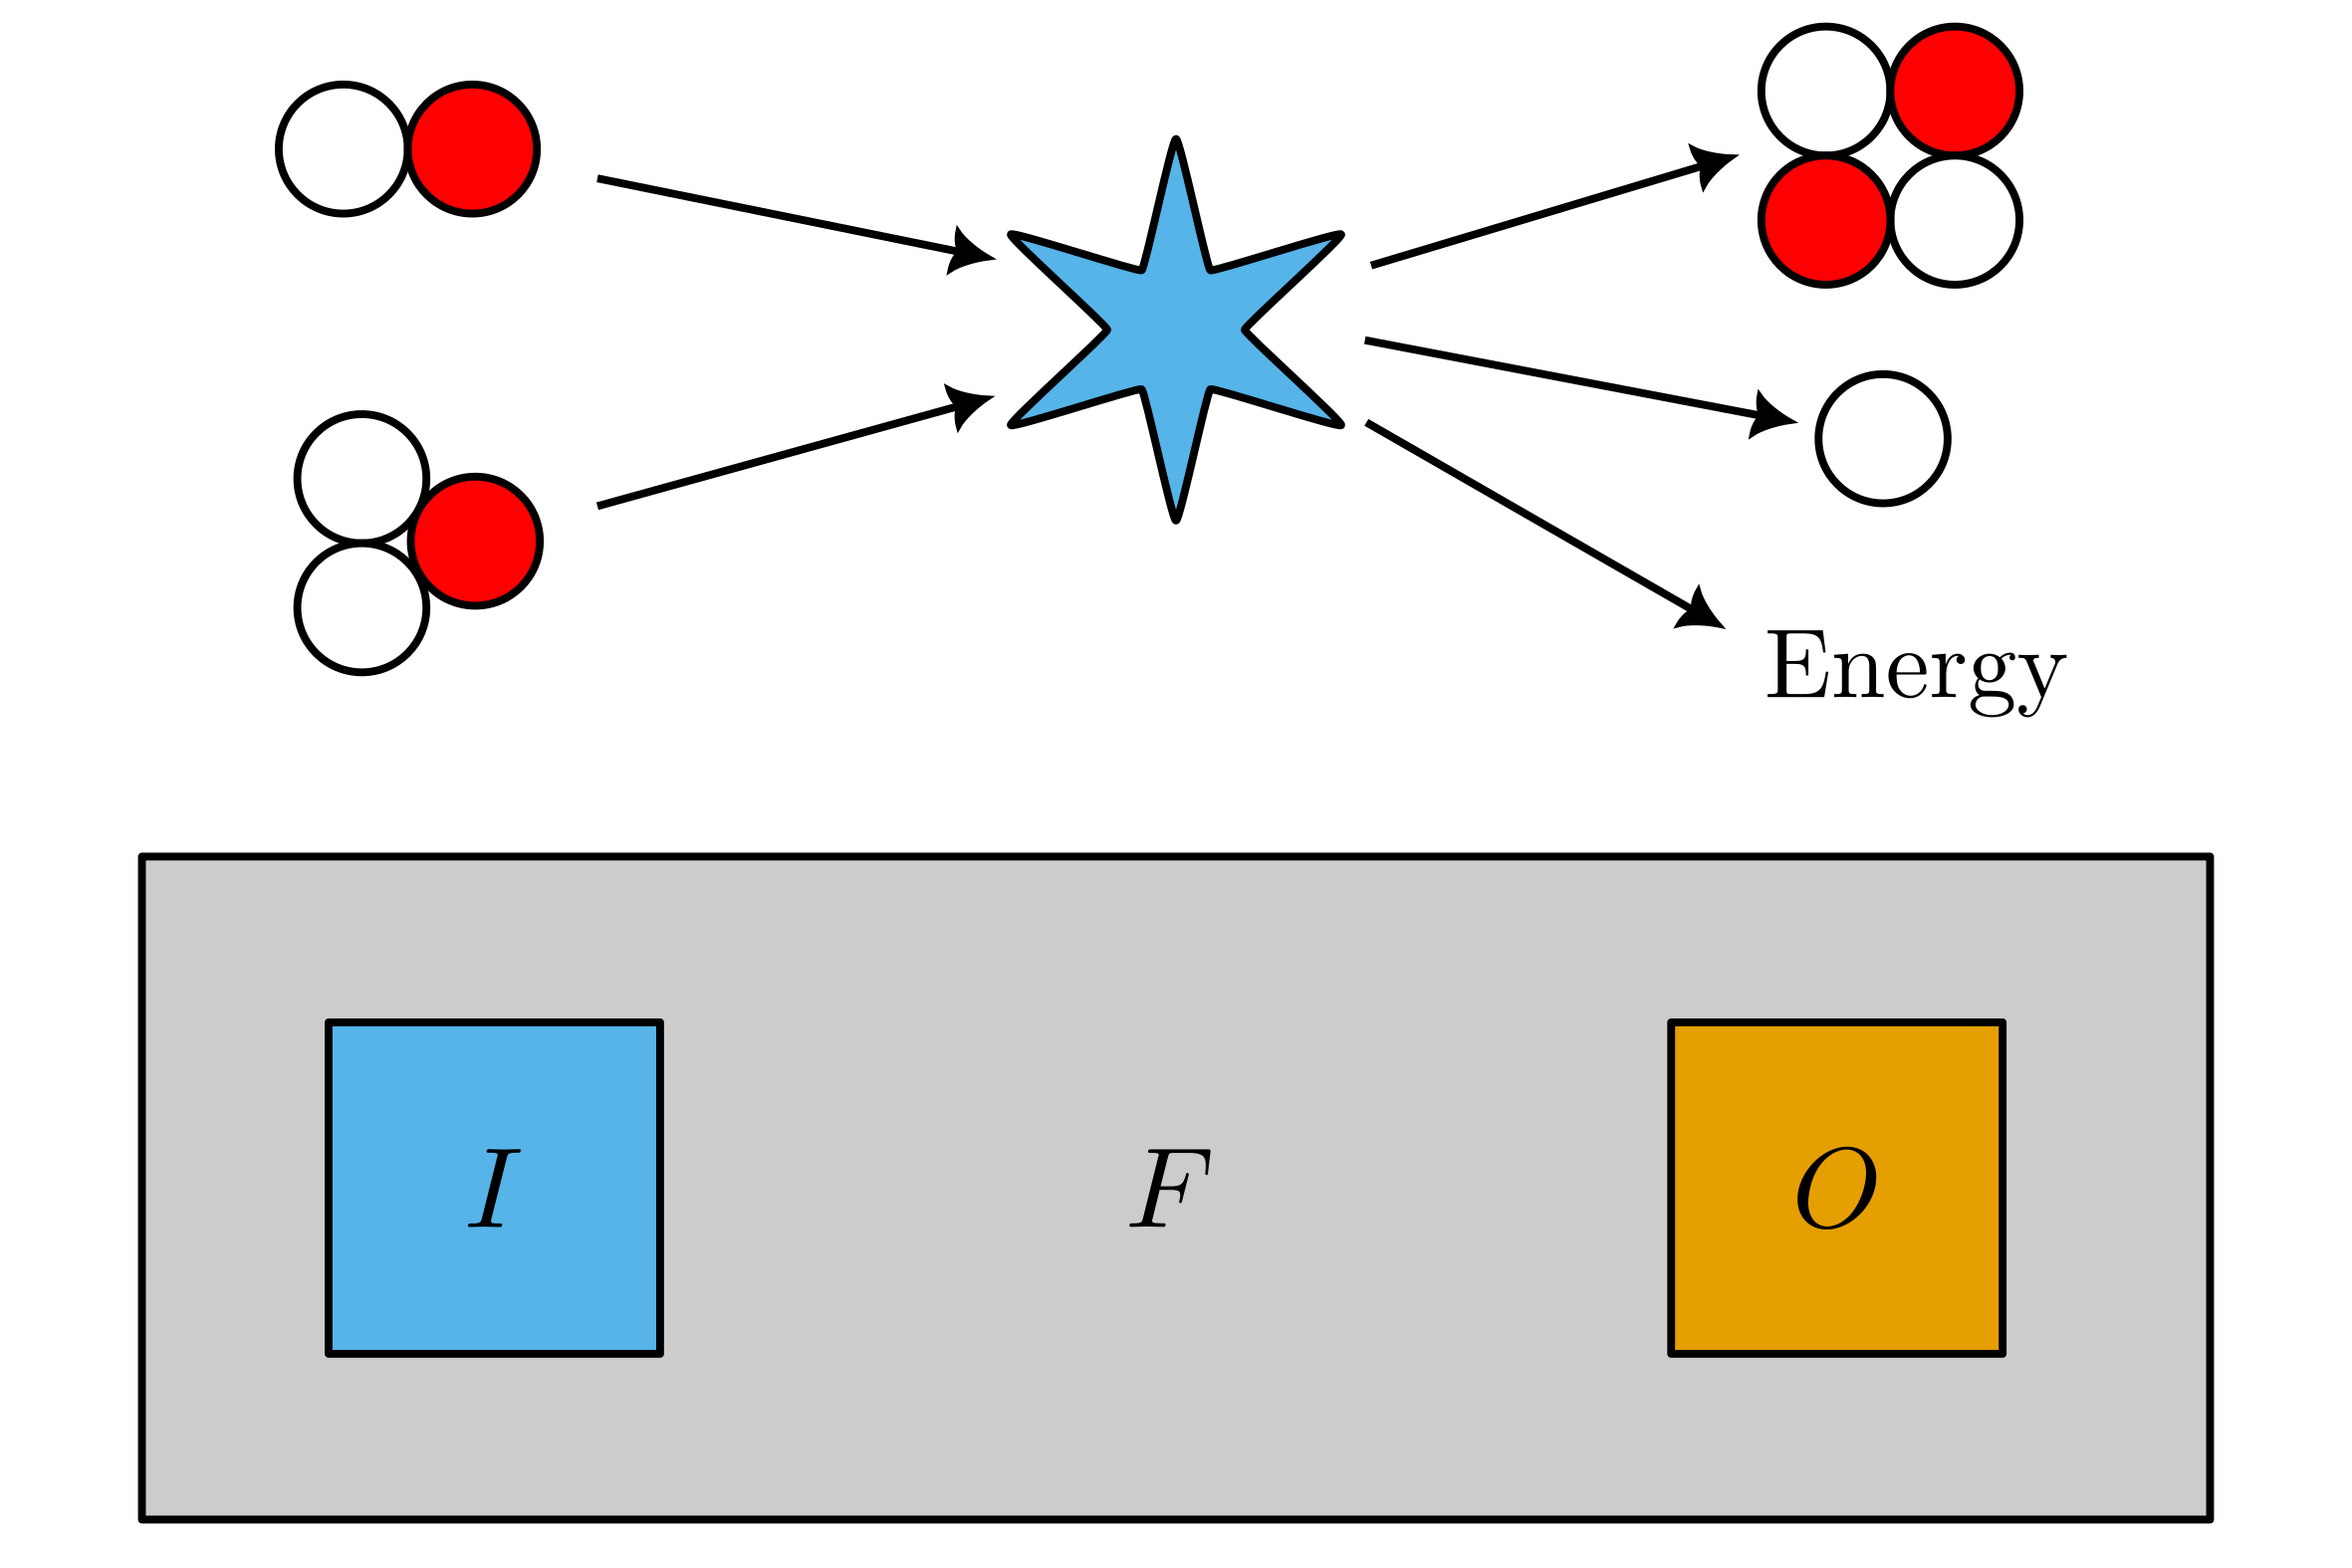
\includegraphics[width=\textwidth]{Figure 6.8.A}
\caption{An abstraction of hydrogen fusion modeled using computable functions}
\end{figure}
\noindent
If $q$ is our probability to fail to detect fusion with a single experiment, then $1-q^n$ is the probability we will have at least one path if we search via $n$ random experiment assuming that the fusion is possible. If there is a Boolean mechanical simulation that represents the fusion of two hydrogen atoms into a helium atom plus energy, then computational complexity is of direct relevance to physics and engineering. 
Our goal is to manufacture some machine $F$ that makes a desired target state more likely. A helium fusion project would have an estimated cost of around $\$ 70$ billion USD. 

If the target state can be reached with non-zero probability for an arbitrary noise function, then there exists a method to restrict a boundary noise function to increase or decrease the probability of the target state. In this case, the \textit{computational complexity} determines how long it takes to search for the initial conditions $I$ and machines $F$ that make a desired target state in $O$ more likely.

Computer simulations of helium fusion imply that it is computable function. In that sense, designing a cost-effective helium fusion machine has a computational complexity that depends on how efficiently we are searching. Assuming a solution exists, different search algorithms have differing levels of how long a problem takes to solve.

Suppose that we have a sorting algorithm for $n$ inputs. We say that asymptotically as $n \rightarrow \infty$ that the algorithm has a best-case time complexity of $\Omega(n)$, an average-case time complexity of $\Theta(n \log n)$, and a worst-case time complexity of $O(n^2)$. Time complexity refers to how the algorithm's duration scales with input size $n$. An algorithm with worst-cast time complexity of $1000 n^2$ is considered an $O(n^2)$ algorithm because we are interested in how the time scales as our input size $n$ scales, usually as $n \rightarrow \infty$. Most evaluations of how useful an algorithm is stated in worst-case complexity due to human cognitive bias for determinism.

The computational complexity class \textbf{P} refers to the set of all decision problems that may be solved by a deterministic Turing machine, or deterministic algorithm with a worst-case time complexity no greater than $O(n^k)$, $k \in \mathbb N$. We call this \textbf{polynomial time complexity}\index{polynomial time complexity} as we implicitly assume our computer or algorithm to be deterministic as opposed to stochastic (non-deterministic). A problem with an algorithm in \textbf{P} is informally considered to be quite fast to solve, especially compared to exponential time complexity of $O(e^n)$.

The computational complexity class $\textbf{NP}$ refers to the set of all decision problems that may be solved by a non-deterministic Turing machine, or non-deterministic algorithm with a worst-case time complexity no greater than $O(n^k)$, $k \in \mathbb N$. We call this \textbf{non-deterministic polynomial time complexity}\index{non-deterministic polynomial time complexity}. We know that \textbf{P} is contained in \textbf{NP}, $\textbf{P} \subseteq \textbf{NP}$, but we do not know if \textbf{P} contains \textbf{NP}, $\textbf{P} \supseteq \textbf{NP}$. If $\textbf{P} contains \textbf{NP} \cap \textbf{P} \supseteq \textbf{NP}$, then $\textbf{P} = \textbf{NP}$.

An \textbf{NP}-complete problem is a problem whose solution may be brute-force searched by guessing and checking via an algorithm in \textbf{NP} but whose correct solution may be verified by an algorithm in \textbf{P}. The puzzle game \textit{Numberlink} is a prominent example:
\begin{figure}[H]
\centering
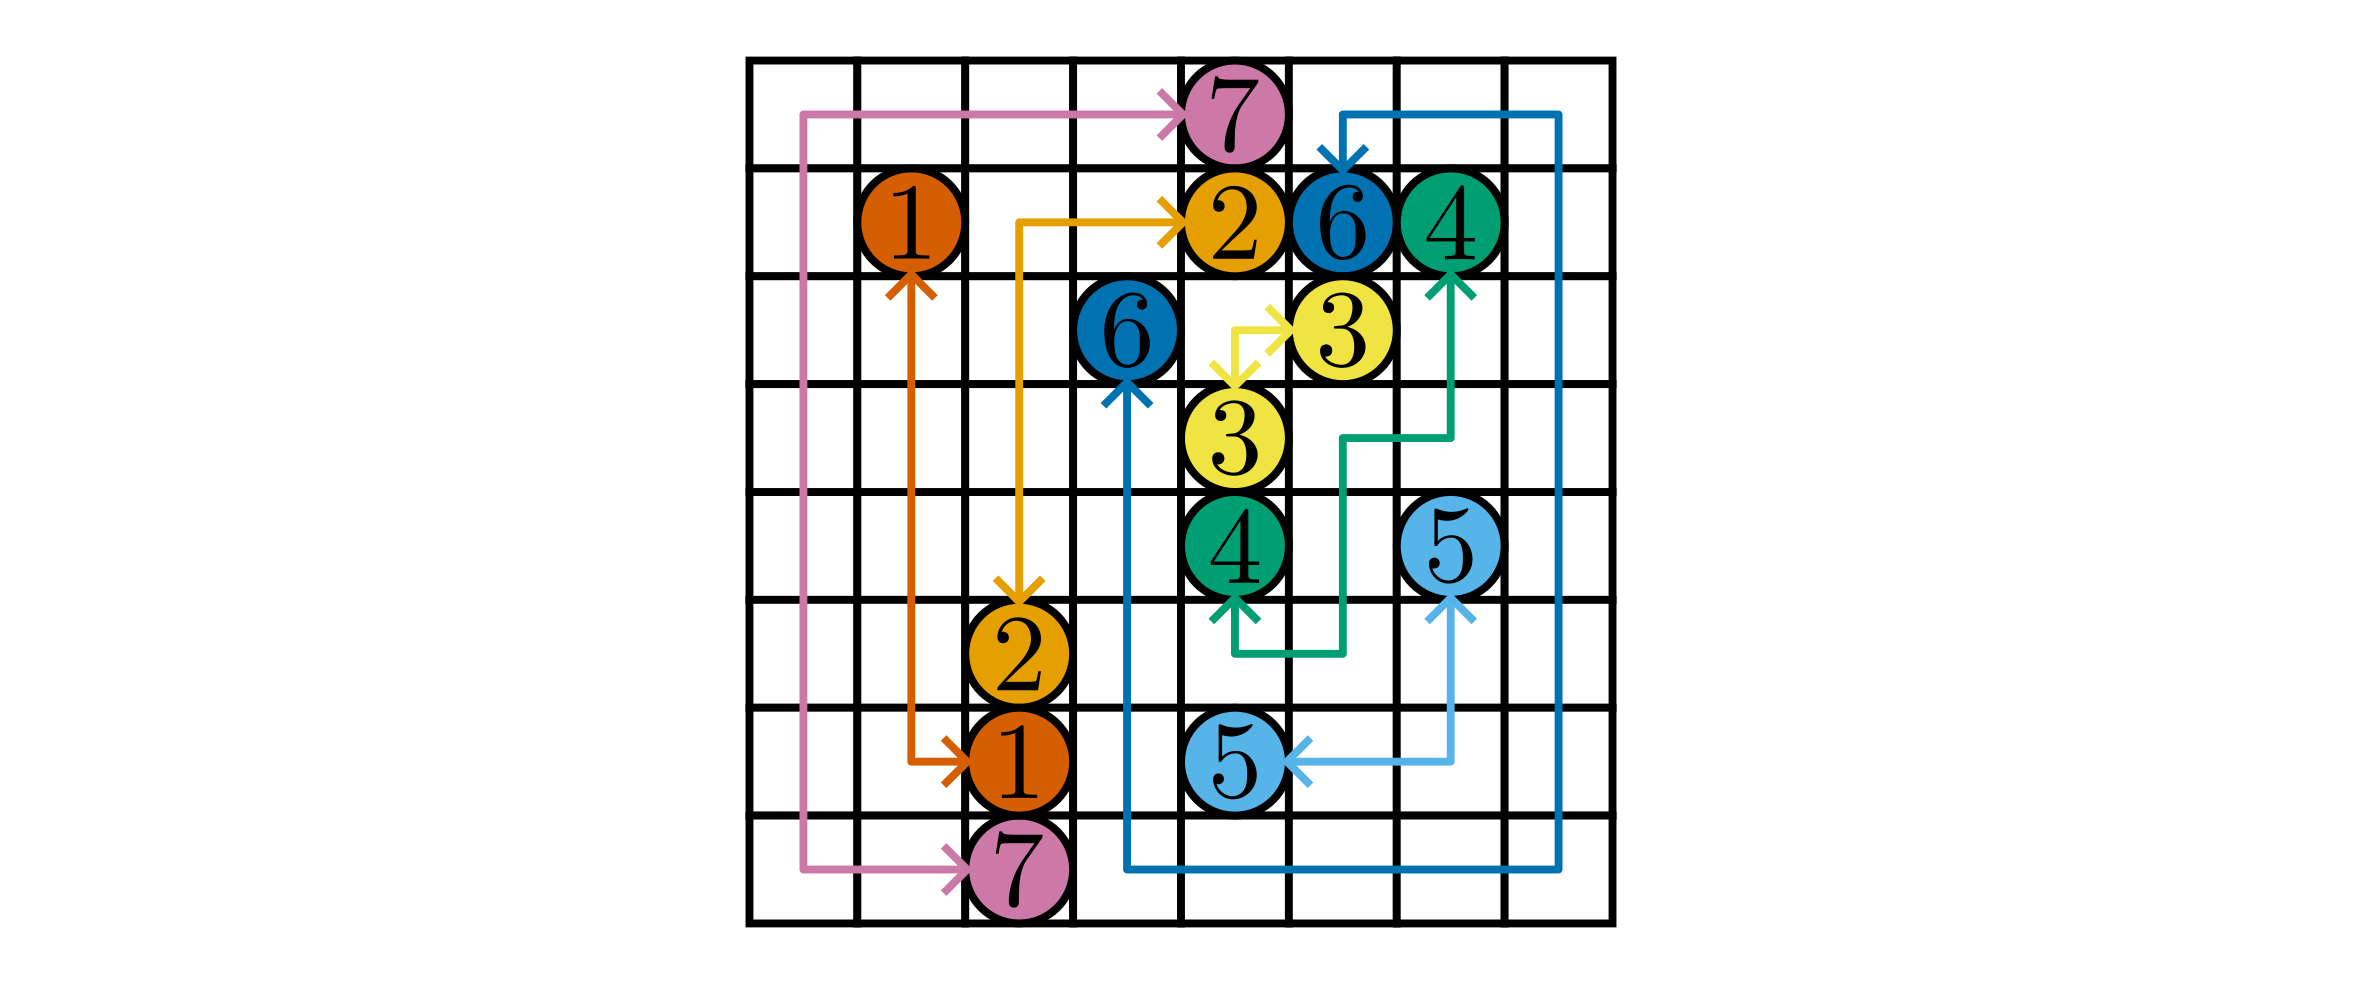
\includegraphics[width=\textwidth]{Figure 6.8.B}
\caption{A Numberlink game using all Okabe-Ito colorblind colors}
\end{figure}
\noindent
It is not necessary to fill all cells or to have a unique solution to be \textbf{NP}-complete. If $\textbf{P} = \textbf{NP}$, then searching can be as fast as checking. If $\textbf{P} \subset \textbf{NP}$ only, then searching will never be faster than checking.

The 3D Ising model and Boolean random walks are both \textbf{NP}-complete. The Ising model is exactly solvable in the $2$-dimensional case, or the planar case, with or without an external magnetic field, but the Ising model in the $3$-dimensional case with an external magnetic field is computationally intractable. Boolean random walks is \textbf{NP}-complete due to requiring maximal independent sets.

The computational complexity classes \textbf{PP} and \textbf{BPP} introduce errors and refer to the set of all decision problems that may be solved by a probabilistic Turing machine or probabilistic algorithm. Probabilistic polynomial (\textbf{PP}) has a worst-case time complexity of $O(n^k)$ and error probability of $\varepsilon <\frac{1}{2}$ per run. Bounded-error probabilistic polynomial (\textbf{BPP}) has a worst-case time complexity of $O(n^k)$ and error probability of $\varepsilon <\frac{1}{3}$ per run. 

A computational problem with an algorithm in \textbf{BPP} is considered efficient to solve on a real computer. This is because we can layer any \textbf{BPP} algorithm with a majority algorithm. Assuming that any individual \textbf{BPP} algorithm solver is dramatically faster than its deterministic verification algorithm in \textbf{P}, random majority verification is fast and reliable due to exponentially decreasing error.

\chapter{Graph Theory}

\section{Motivations for Learning Graph Theory}
\textbf{Graph theory}\index{graph theory} is the study of graphs, more commonly known as networks. A graph represents how a \textit{vertex} is connected to any other vertex via an \textit{edge}. Graphs are ideal for representing road networks, and shortest path algorithms help people travel quickly in unfamiliar places. Graphs can do more than relate physical objects, helping us define relations between mental objects. At a philosophical level, all objects relate themselves to one another in some way, else we would not be able to distinguish between them. Graphs are composed of countable objects, but even continuous objects can still be analyzed via graph theory.

A surface or topology such as a donut, if divided into triangular faces $F$ using vertices $V$ connected by edges $E$ will always have the same Euler characteristic $\chi$. This does not depend on how many polygonal faces are used:
\begin{figure}[H]
\centering
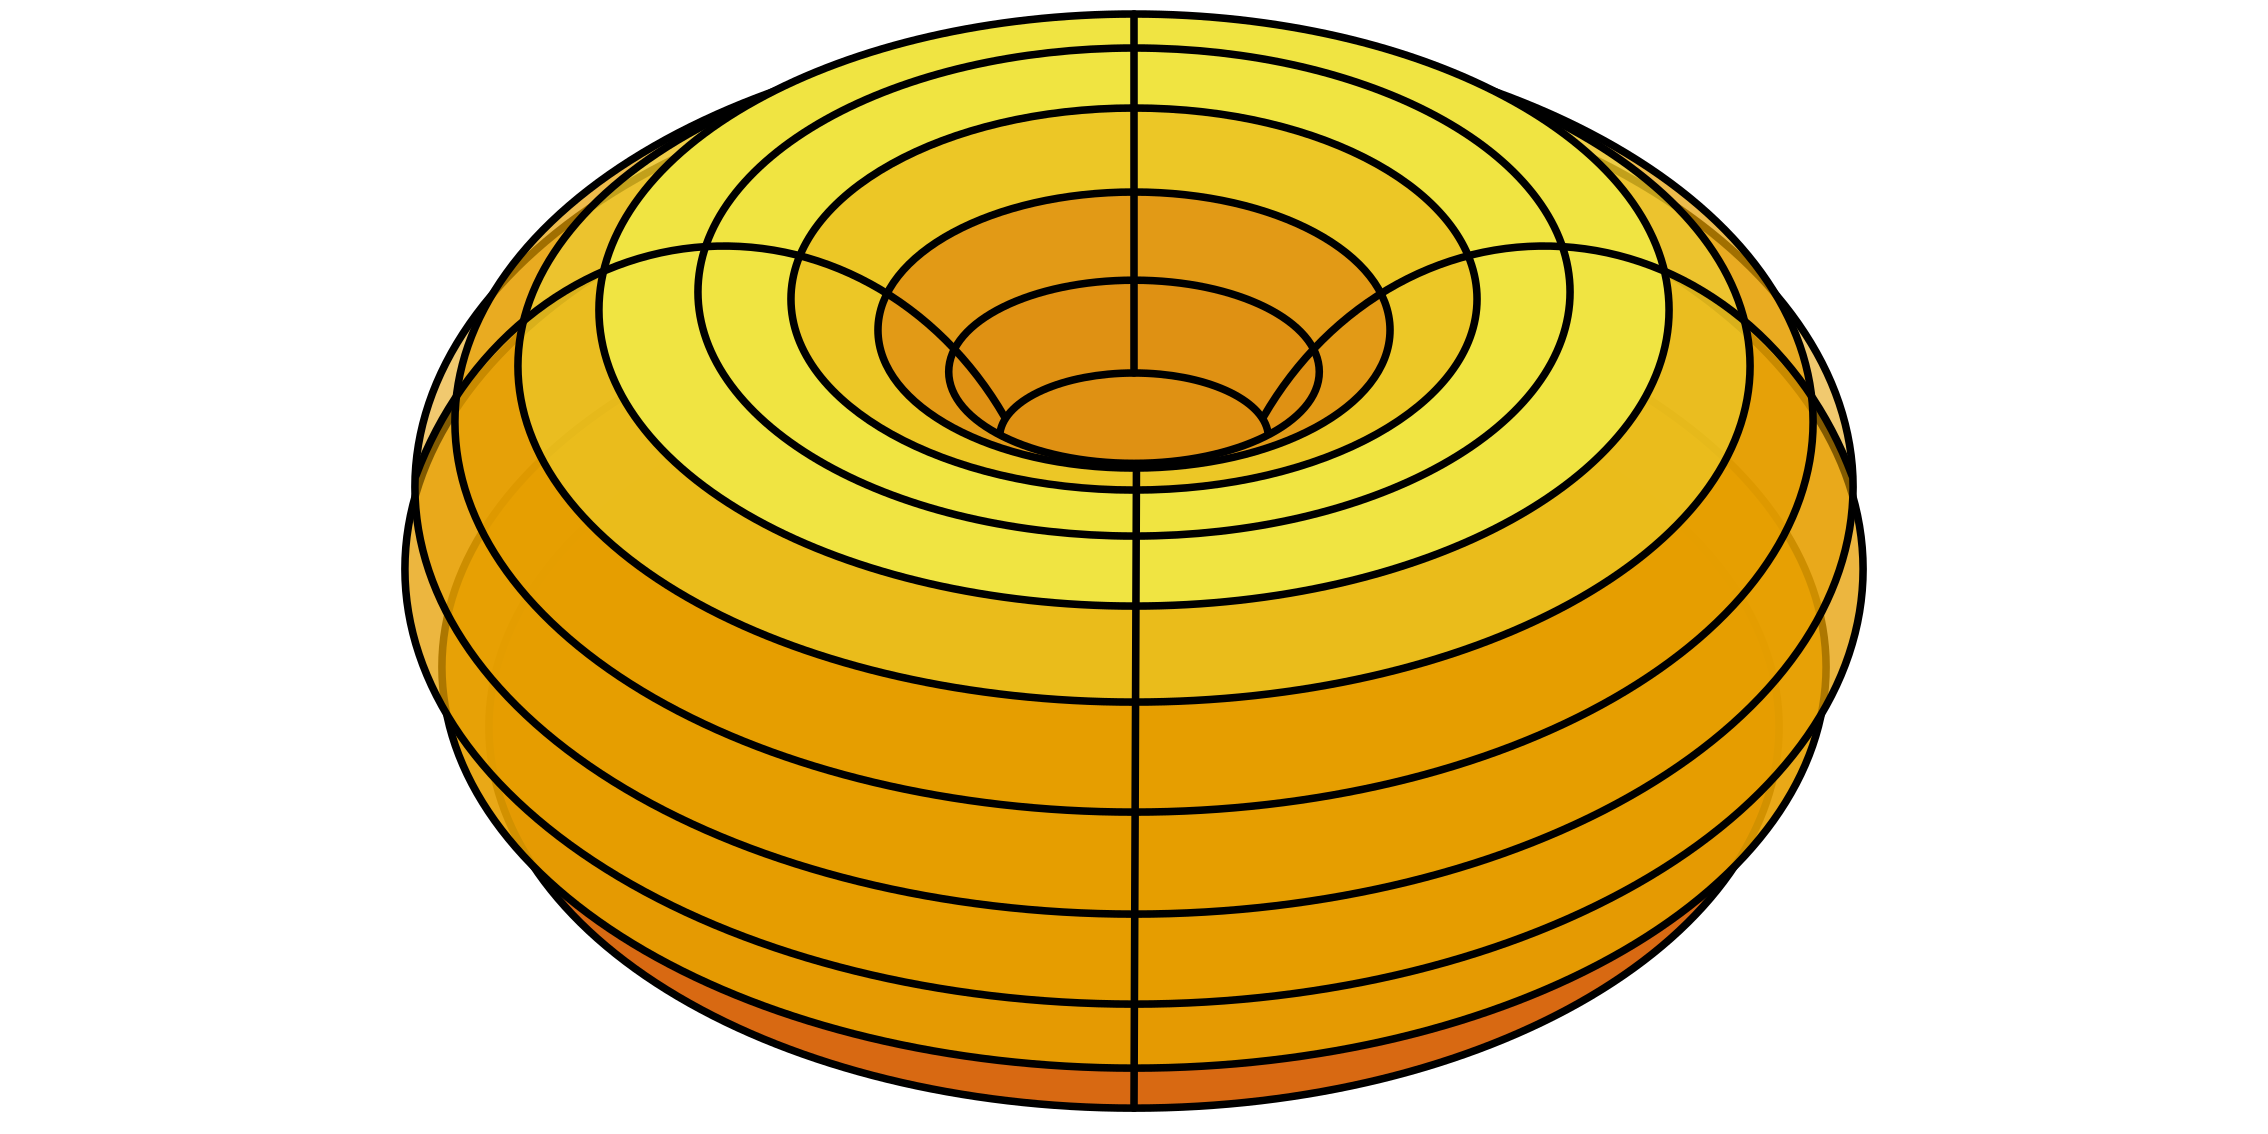
\includegraphics[width=\textwidth]{Figure 7.1.A}
\caption{A 3D mesh of a torus composed of curved rectangular faces}
\end{figure}
\noindent
In the image, the torus connects its faces along the edges, and lines/edges themselves connect vertices/points. The most famous example of the application of graph theory to continuous objects is the Euler characteristic:
$$\chi = V - E + F$$
Subdividing any rectangular face on the donut always creates more edges and vertices such that the Euler characteristic does not change. Likewise, deleting edges and vertices removes faces such that the Euler characteristic does not change. It is a common joke that a topologist does not know the difference between a donut and a coffee mug because they share the same Euler characteristic value $\chi$. 

Computers are used in the real world to relate mental objects, which is helpful because mental objects are much easier to move around than physical objects. The vague and general nature of computers and networks of information is precisely what makes computers so useful. It is no coincidence nor accident that neuron clusters and galactic clusters are likewise structured in the same way as computer networks and road networks. They all represent channels of information, meaning it is inaccurate to say that a neural signal is less real than a vehicle.

Graph theory is fundamental to games like chess or Go (weiqi) with an obvious example of discrete states. The game may only progress through a series of states that obey some transition rule. Given that the brains of individuals players are composed of particles that move randomly, each game of chess or Go technically obeys the rule of a probabilistic Turing machine. Even if a computer's written algorithm is $99.9\%$ deterministic, some $0.01\%$ randomness of physical reality is fundamentally irreducible. In a very real sense, random computers are playing a deterministic game. Such games have a vast chain of events before victory is determined such that every game is unique. Will we explore every possible state of chess or weiqi before the universe resets?


\section{Undirected Graphs}
A \textbf{graph}\index{graph} $G$ is a set of vertices $V$ connected via a set of edges $E$. More formally, a graph $G$ is a $2$-tuple such that $G = (V, E)$. An \textbf{undirected graph}\index{undirected graph} is the simplest graph, and it represents whether or not two vertices are joined by edges. 

If $x,y \in V$ and vertex $x$ connects to vertex $y$, then the order does not matter such that $(x,y) = (y,x) = 1$. Else if they are not connected, $(x,y) = 0$. 
We say that $(x,y) \in V \iff (x,y) = 1$.
\begin{figure}[H]
\centering
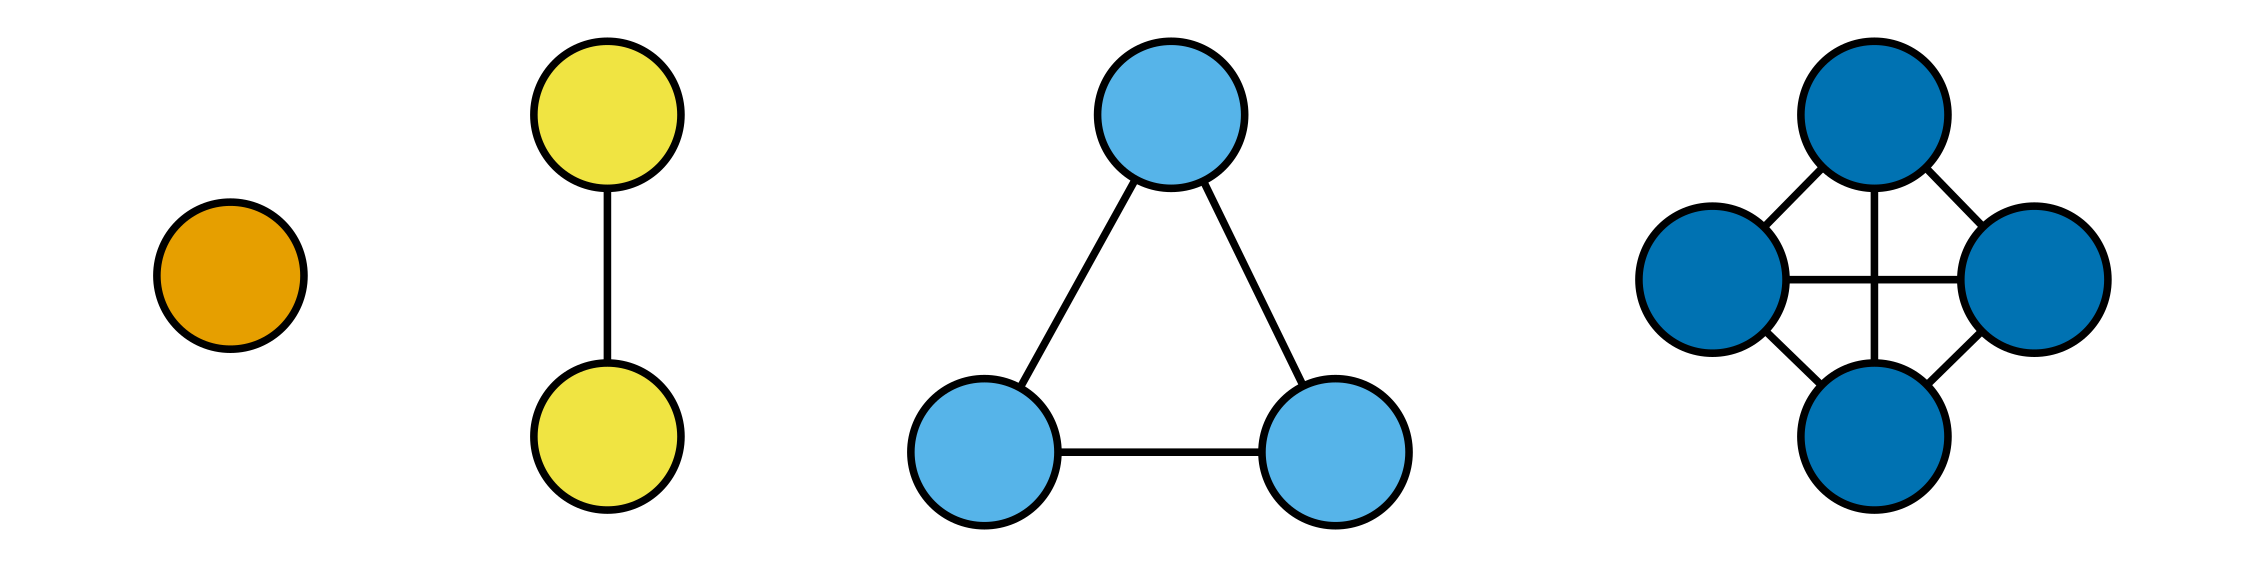
\includegraphics[width=\textwidth]{Figure 7.2.A}
\caption{A set of complete graphs with one, two, three, and four vertices all connected}
\end{figure}
\noindent A set of vertices $V$ with cardinality $|V| = \theta$ has a total of $2^\theta$ valid sets of edges that may form a graph $G$. Vertices that are connected via an edge are said to be \textit{adjacent}, and an edge that connects a vertex to itself is called a \textit{loop}. A graph is a \textit{simple graph} if it contains no self-looping edges such as $(x,x)$.

The state space graph of a Boolean random walk only contains self-loops in a special case:
\begin{figure}[H]
\centering
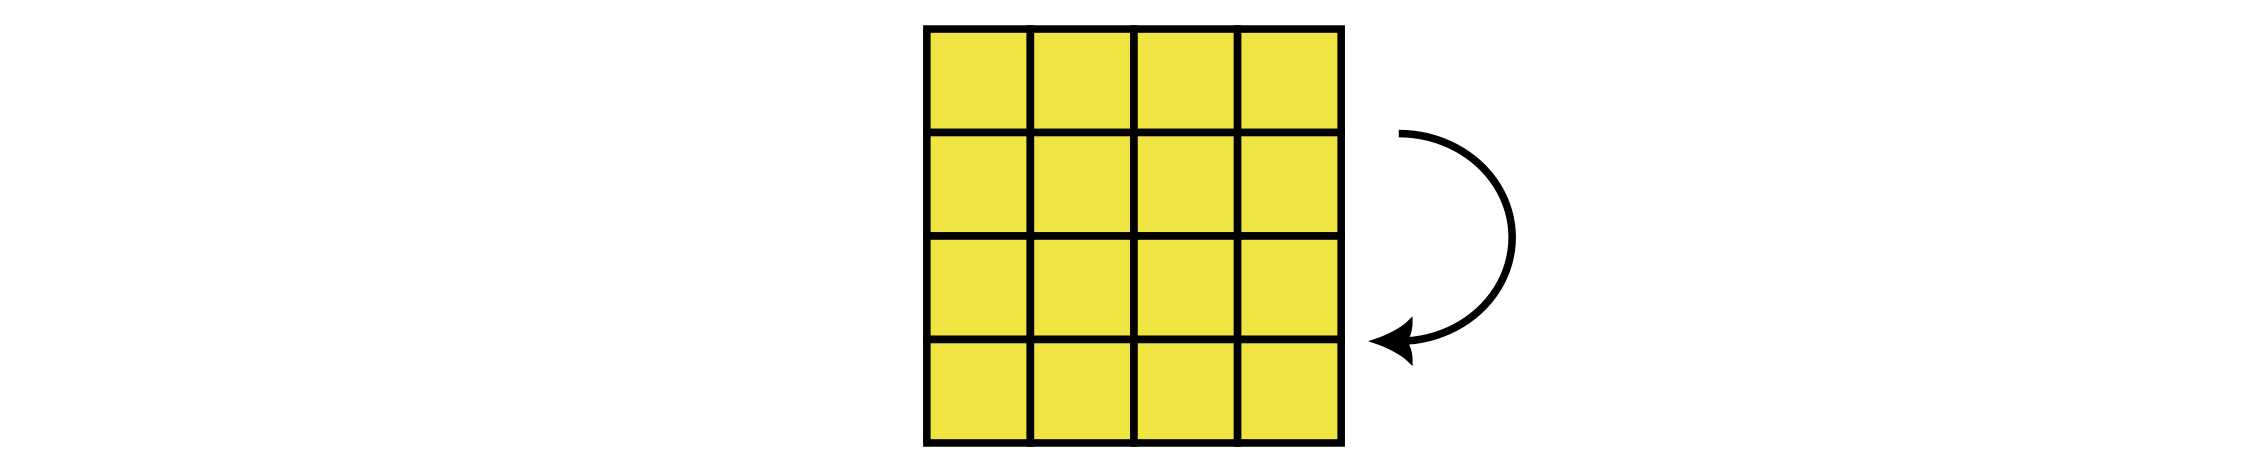
\includegraphics[width=\textwidth]{Figure 7.2.B}
\caption{A degenerate state is a state in which a system cannot recover}
\end{figure}
\noindent
The non-polar state, or wuji state, fails to transition into a new state. Most dynamical systems of interest do not loop in a single time step, or are at least unlikely to.

For example, if we have a $2 \times 2$ Boolean dynamical system with $k=2$ particles and $N-k=2$ antiparticles, then it has ${N \choose k} = \theta$ possible ways to arrange these particles. Since $\theta = 6$, there are $2^\theta$ possible ways to connect these system states. However, a Boolean random walk only allows one of these arrangements to be correct:
\begin{figure}[H]
\centering
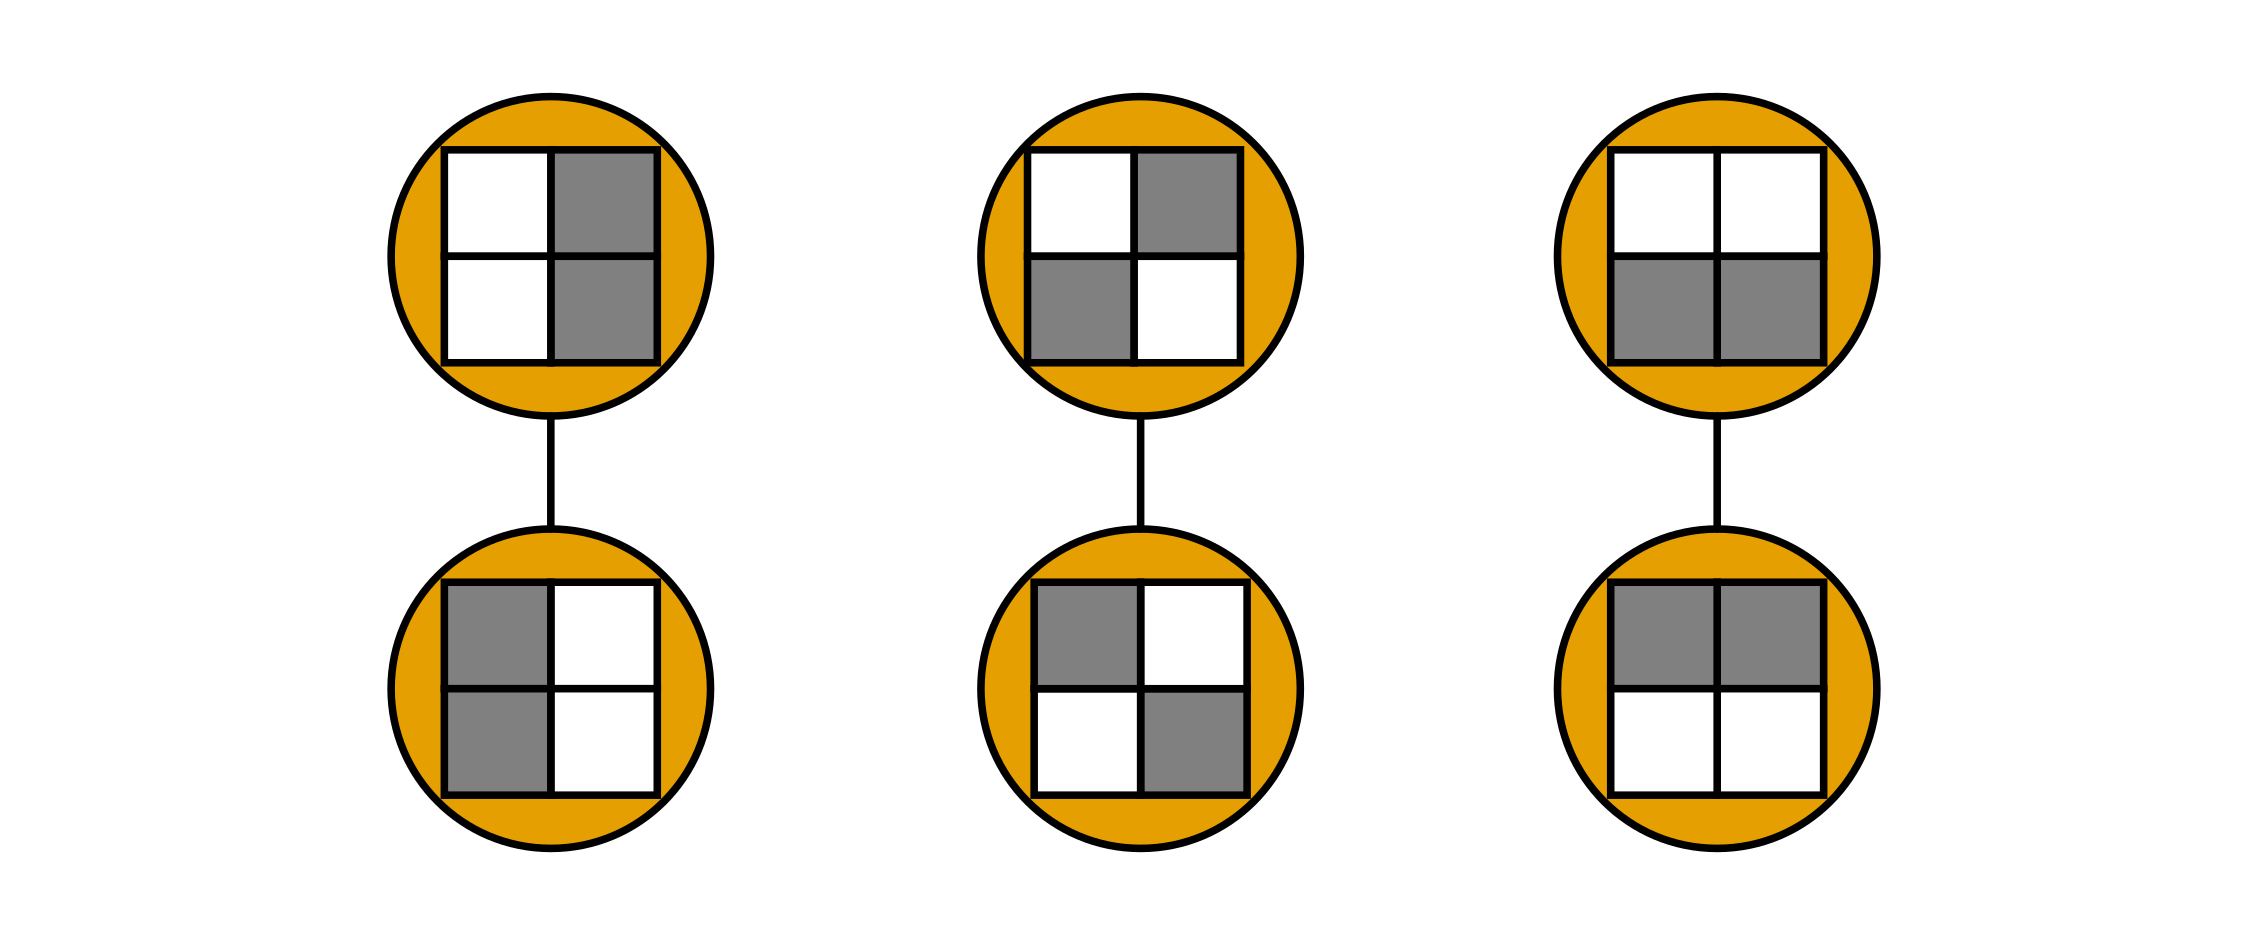
\includegraphics[width=\textwidth]{Figure 7.2.C}
\caption{The state space graph of a 2x2 Boolean random walk with $k=2$ particles and $N-k=2$ antiparticles}
\end{figure}
\noindent
Due to the nature of a Boolean random walk, the number of particles and antiparticles must be preserved. The possible states for the time-evolving system $X_t$ are connected via the state space graph $G = (\mathcal X, A)$ in which $\mathcal X$ is the set of all states and $A$ is the set of connections between states.

Consider a checkerboard state $X_t$ that is transitioning into its inverse $X_{t+1} = -X_t$. How many ways may it get there under a Boolean random walk?
\begin{figure}[H]
\centering
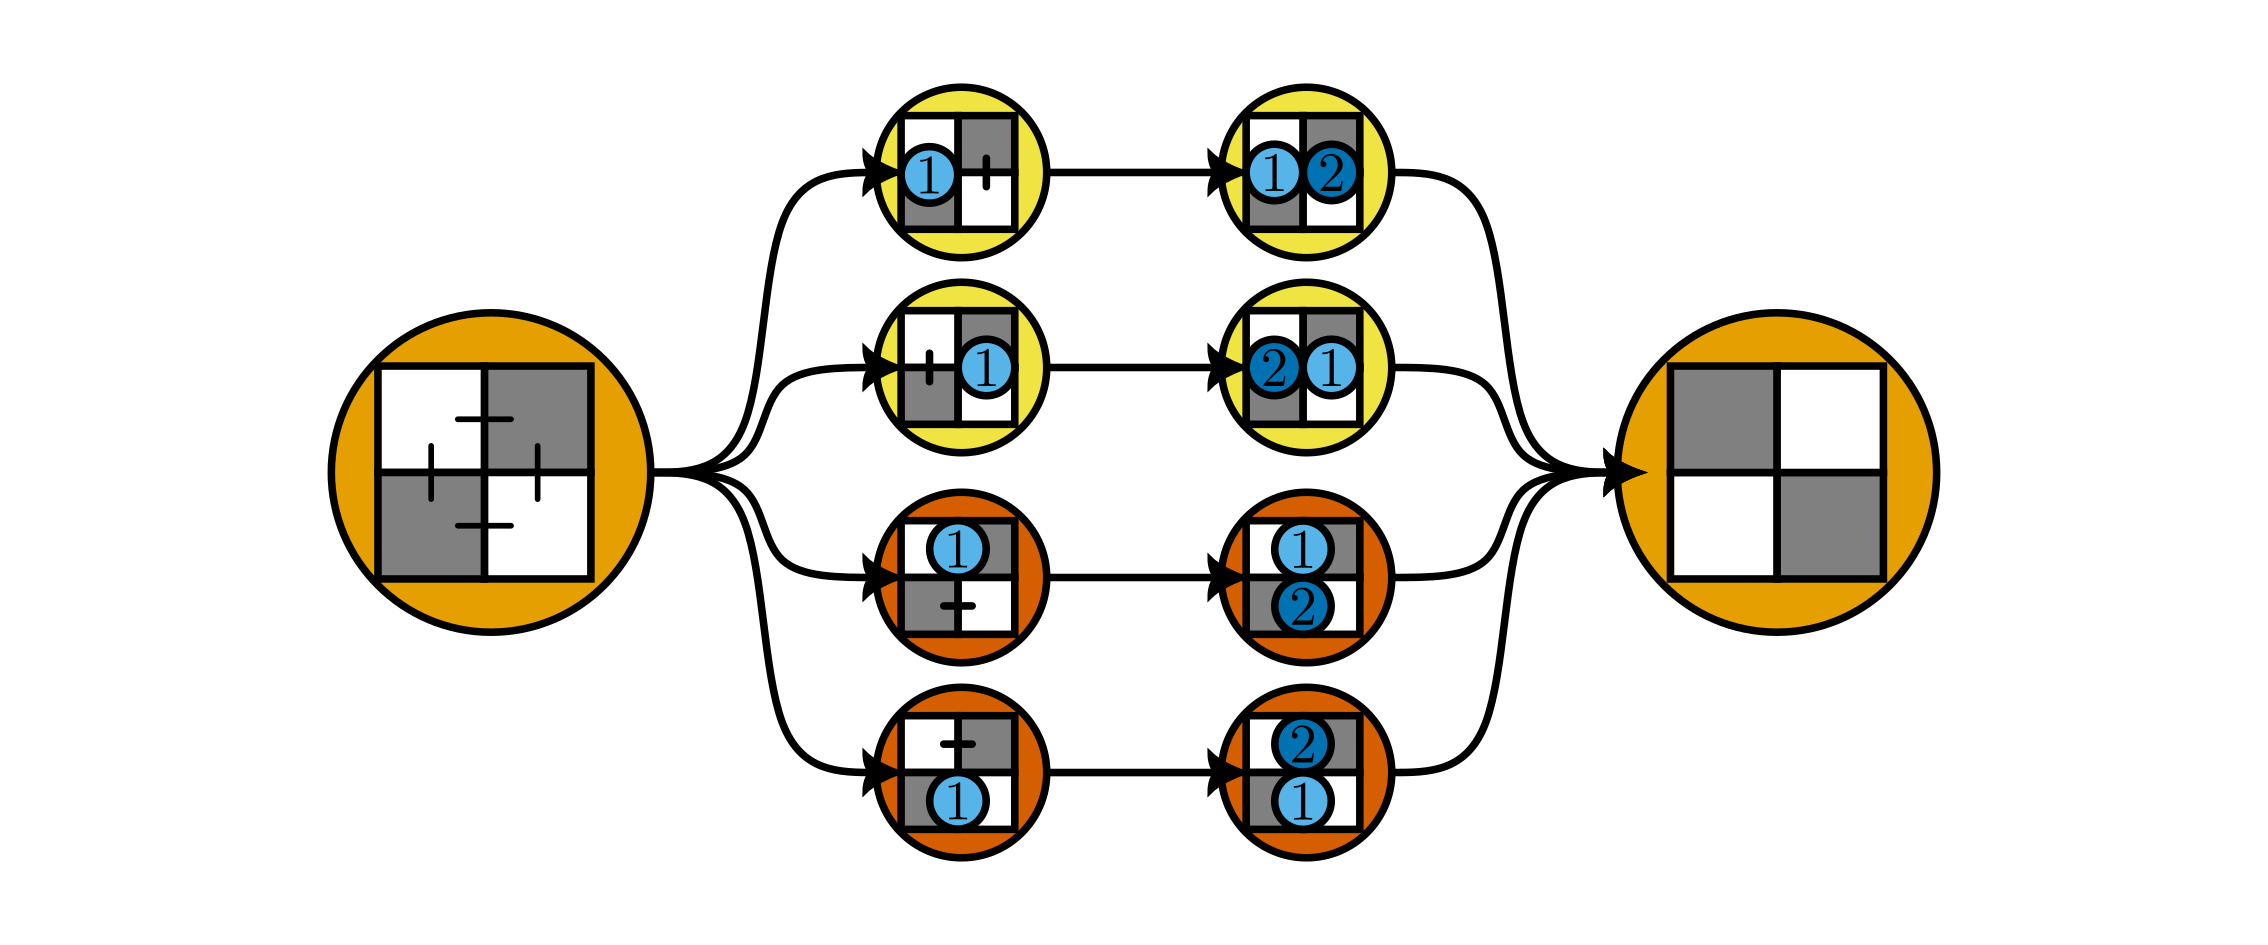
\includegraphics[width=\textwidth]{Figure 7.2.D}
\caption{Multiple possible transitions from the same initial state to the same future state.}
\end{figure}
\noindent
This is a directed graph, which we cover in more detail in \textit{\S 7.3 Directed Graphs}. There are multiple chordings $c$ result in the same transition, but it is unclear how many. However, if there are $n$ particle exchanges, then there are $n! = o$ possible orderings. This ordering is an unintended consequence of the way that we defined determining a transition for a simple random walk as a Boolean random walk: one exchange went first and the others were locked out. 

Within each graph of a Boolean random walk, there are a series of hidden subgraphs within each transition. These subgraphs of $G = (\mathcal X, A)$ can become more refined and specific if you desire. You could even track the \textit{origin identity} of a particle from $X_0$ to $X_t$ for every single particle. However, attempting to calculate detail beyond the transition matrix $P$ for a large system is a fool's errand. It is hard enough to simulate enough data to estimate the transition matrix $P$ of a $3 \times 3$ Boolean mechanical system.

The graph $G$ of a Boolean random walk is a \textbf{partial cube}\index{partial cube}, a cubic lattice with deleted edges. This means that it the subset of a hypercube graph of equal distance between vertices. Suppose that you have the following bounded Boolean random walk of $N = 4 \times 4$. The maximally informative graph possible for a Boolean random walk tracks the \textit{origin identity} of each individual particle assigned at time $t=0$. In this table, we will assign cell values as $f \in \{0, 1\}$ instead of the $\{-1, +1\}$ convention.
\begin{center}
\scalebox{1.0}{\begin{tabular}{|c | c | c | c | c | c | c | c|}
\hline
Index & Origin & Value $f$ & $x_1$ & $x_2$ & $|\Delta_{x_{1}} f|$ & $|\Delta_{x_{2}} f|$ & $t$ \\
\hline
1 & 1 & 1 & 1 & 1 & 1 & 1 & 0\\
2 & 2 & 0 & 1 & 2 & 1 & 1 & 0\\
3 & 3 & 1 & 1 & 3 & 1 & 0 & 0\\
4 & 4 & 1 & 1 & 4 & 0 & 0 & 0\\
\vdots & \vdots & \vdots & \vdots & \vdots & \vdots & \vdots &\vdots\\
16 & 16 & 0 & 4 & 4 & 0 & 0 & 0\\
\hline
\end{tabular}}
\end{center}
Such a maximally informative graph is the subset of the $N$-th Cartesian product of independent, non-interacting random walks like so:
\begin{figure}[H]
\centering
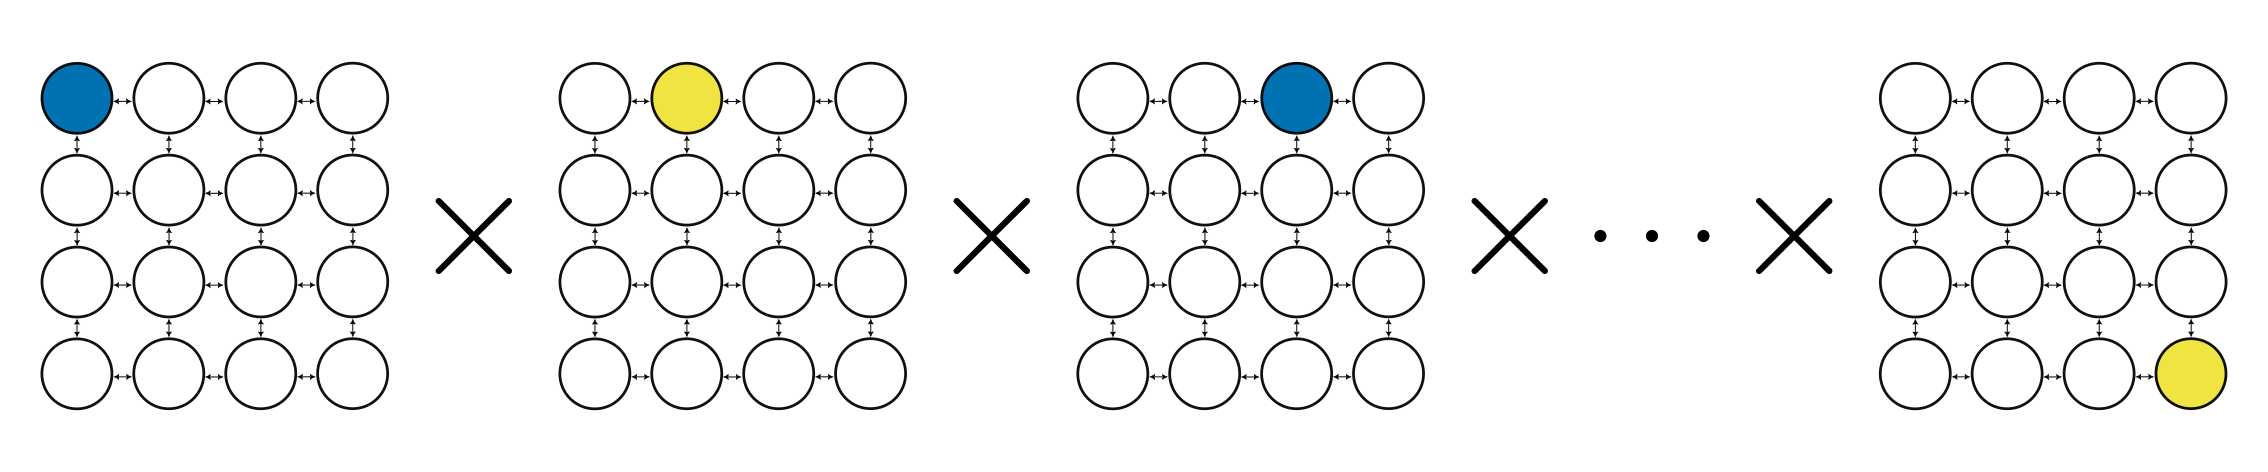
\includegraphics[width=\textwidth]{Figure 7.2.E}
\caption{The product of independent random walks gives a superset of possible Boolean random walk states}
\end{figure}
\noindent 
For example, $(1, 2, 3, 7)$ is a sequence describing the origin identity at time $t=3$ for the cell at index 7. This level of detail is unnecessarily informative because we treat particles as identical under the transition function. If we are not tracking \textit{origin identity}, the graph $G$ is flattened across the origin identity dimension with respect to Boolean value $\mathbb B$.

A \textbf{hypergraph}\index{hypergraph} $G$ generalizes edges to hyperedges $E$, which may connect any number of vertices $V$. 
\begin{figure}[H]
\centering
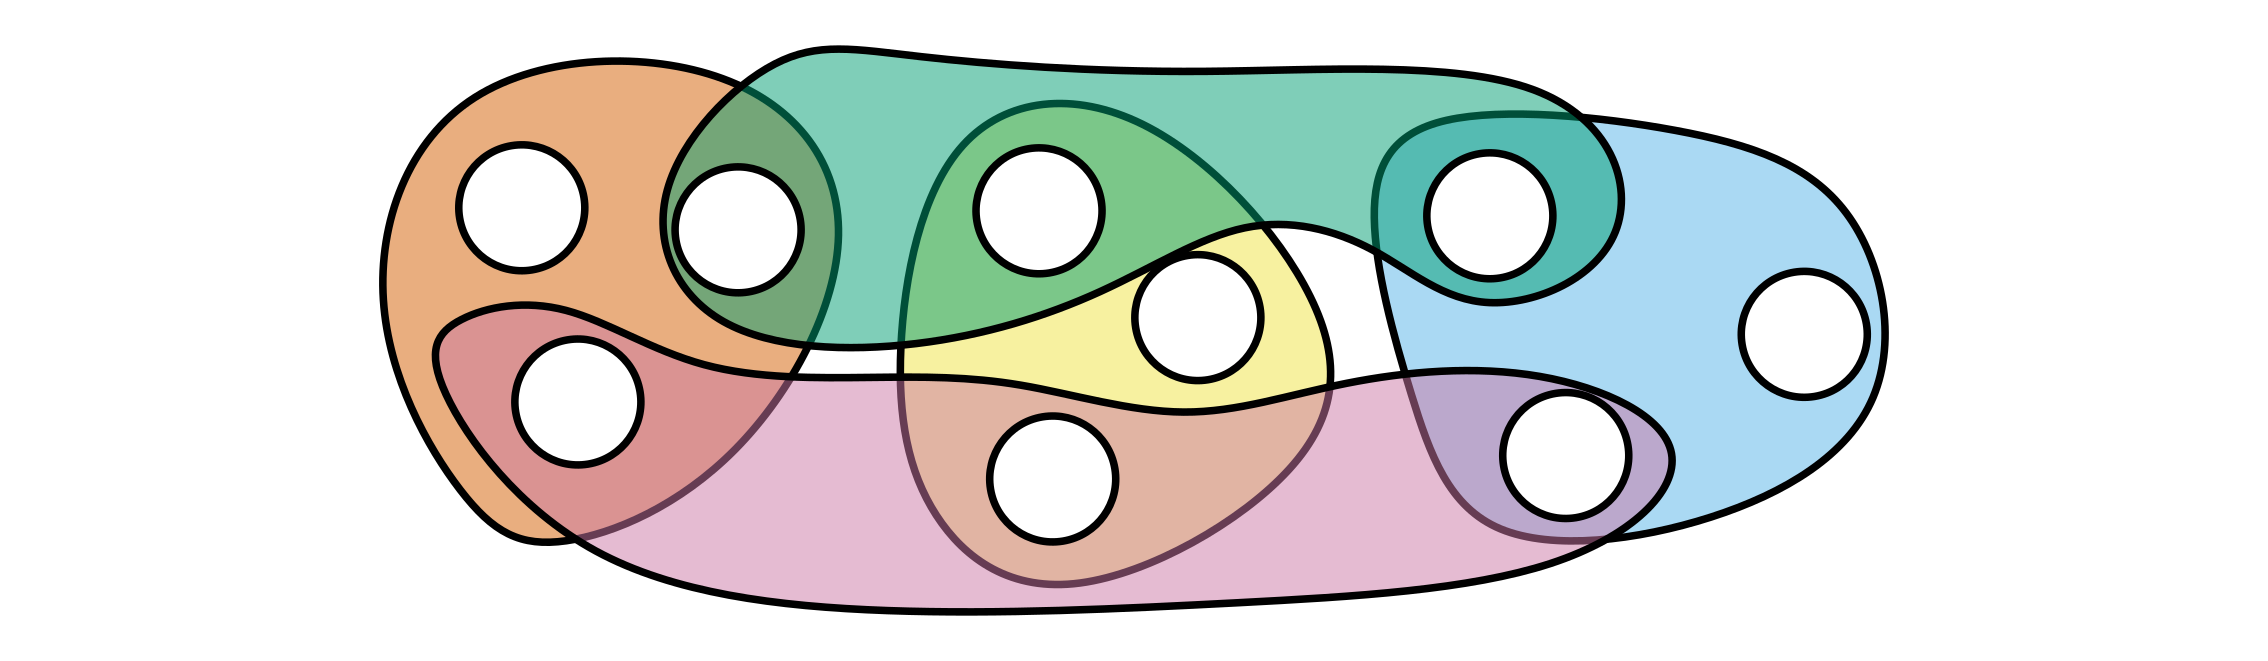
\includegraphics[width=\textwidth]{Figure 7.2.F}
\caption{Colored hyperedges join together multiple vertices at a time}
\end{figure}
Consider a specific Boolean random walk $X$: the cells are vertices $V$ and the potential connections between them as edges $E$, and we get a graph $G$. 
\begin{figure}[H]
\centering
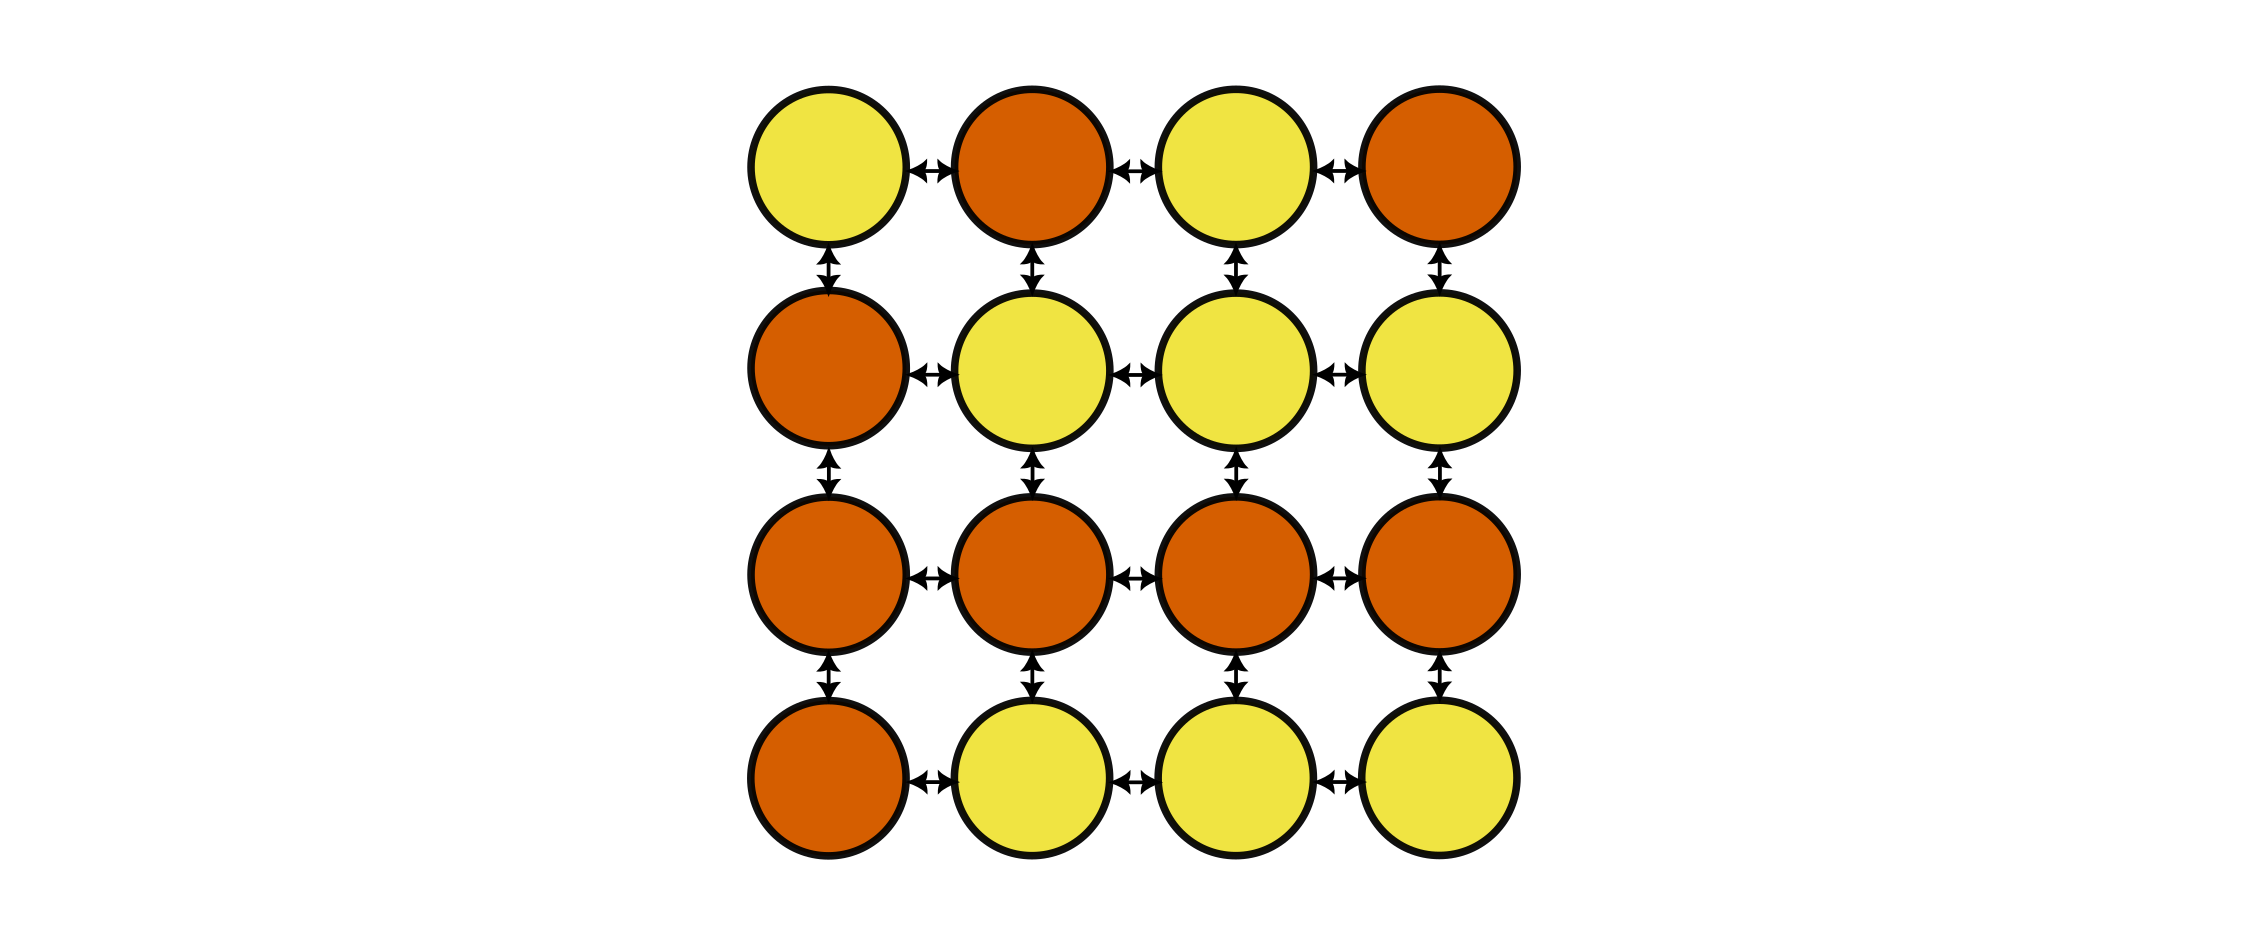
\includegraphics[width=\textwidth]{Figure 7.2.G}
\caption{The cell/graph form of a Boolean random walk}
\end{figure}
Consider instead the forward difference $\Delta X$: the potential connections between cells as vertices $V$ and the cells as hyperedges $E$, we get a hypergraph $G$. 
\begin{figure}[H]
\centering
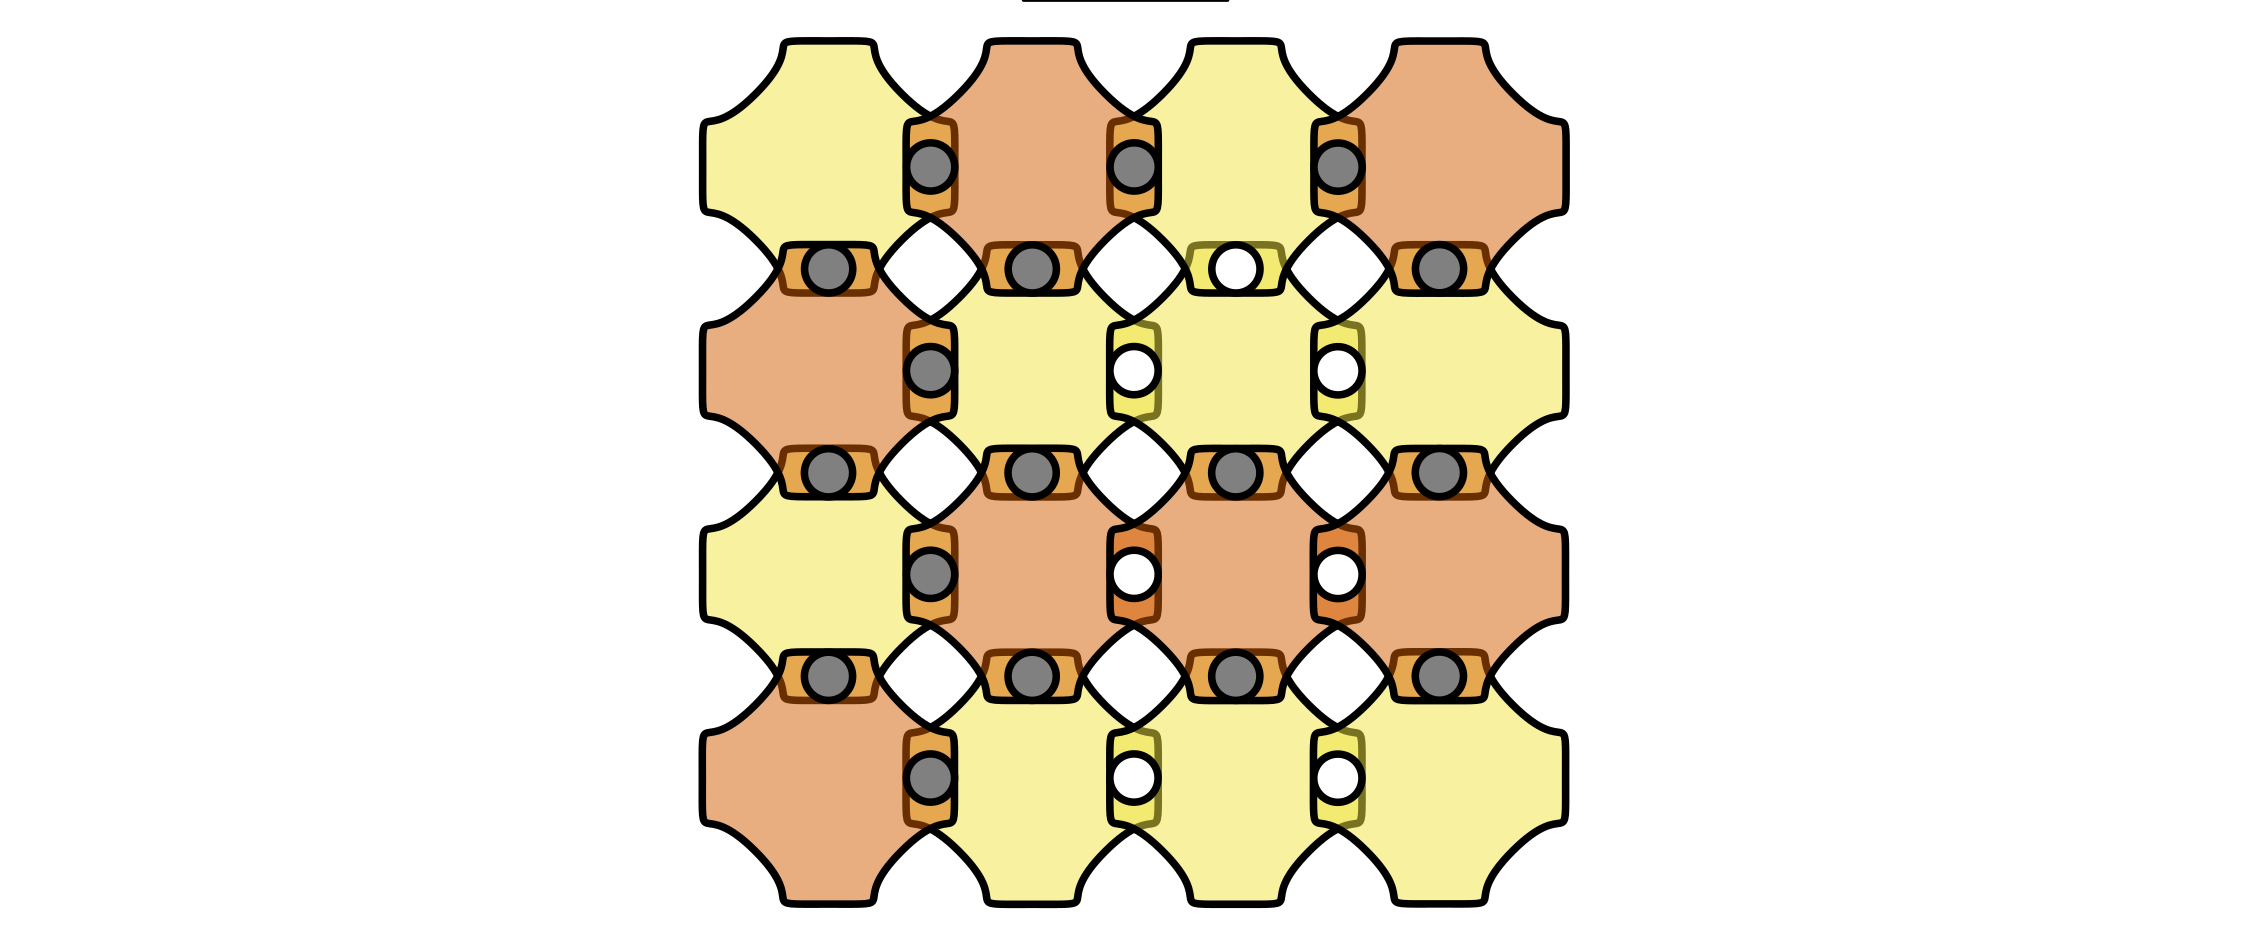
\includegraphics[width=\textwidth]{Figure 7.2.H}
\caption{The hypergraph form of a Boolean random walk}
\end{figure}
\noindent
In the hypergraph form, a valid Boolean random walk transition requires sampling a vertex, then disabling all vertices from any hyperedge that vertex connects to. A single Boolean cell can be represented as a hyperedge, and the hyperedge it itself a subset of a complete graph.

We may however still wish to represent $\Delta X$ using a graph instead of a hypergraph since it is useful to visualize a finite-difference mesh using diamonds/octahedrons for its topological properties as discussed in \textit{\S 7.8 Discrete Topology}:
\begin{figure}[H]
\centering
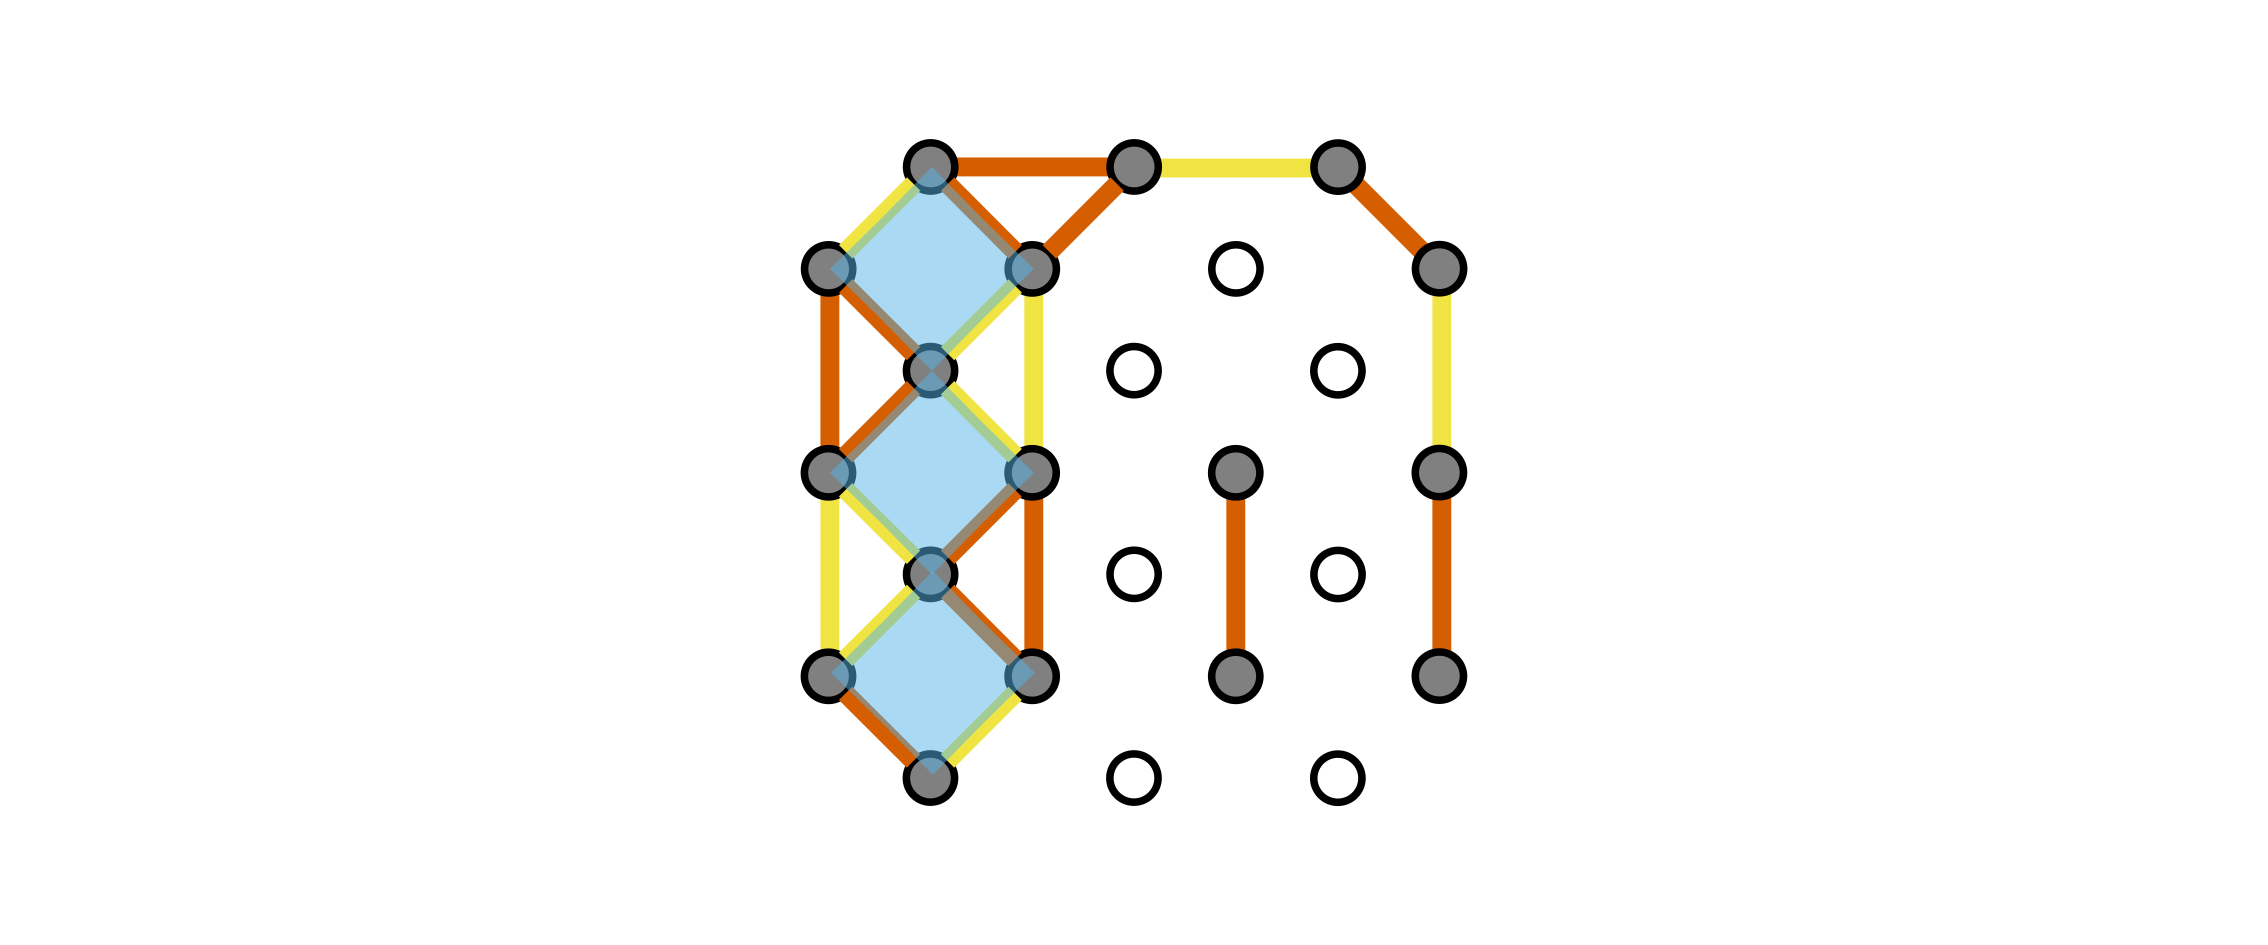
\includegraphics[width=\textwidth]{Figure 7.2.I}
\caption{The finite-difference mesh graph creates diamonds with which to check for long-range dependency via checker chains}
\end{figure}
Here we can see how a finite-difference mesh diagonally across a cube's face is derived from an octahedron. We may turn a hypergraph into a graph by coercing hyperedges into edges, but we needed to draw both cardinal and diagonal edges. This visualization is quite cumbersome to parse, but it has some advantages.

The finite-difference mesh of a 3D checker pattern would generate a tesselation in 3D would consist of octahedrons and tetrahedrons. In the following figure, cardinal edges are omitted for clarity:
\begin{figure}[H]
\centering
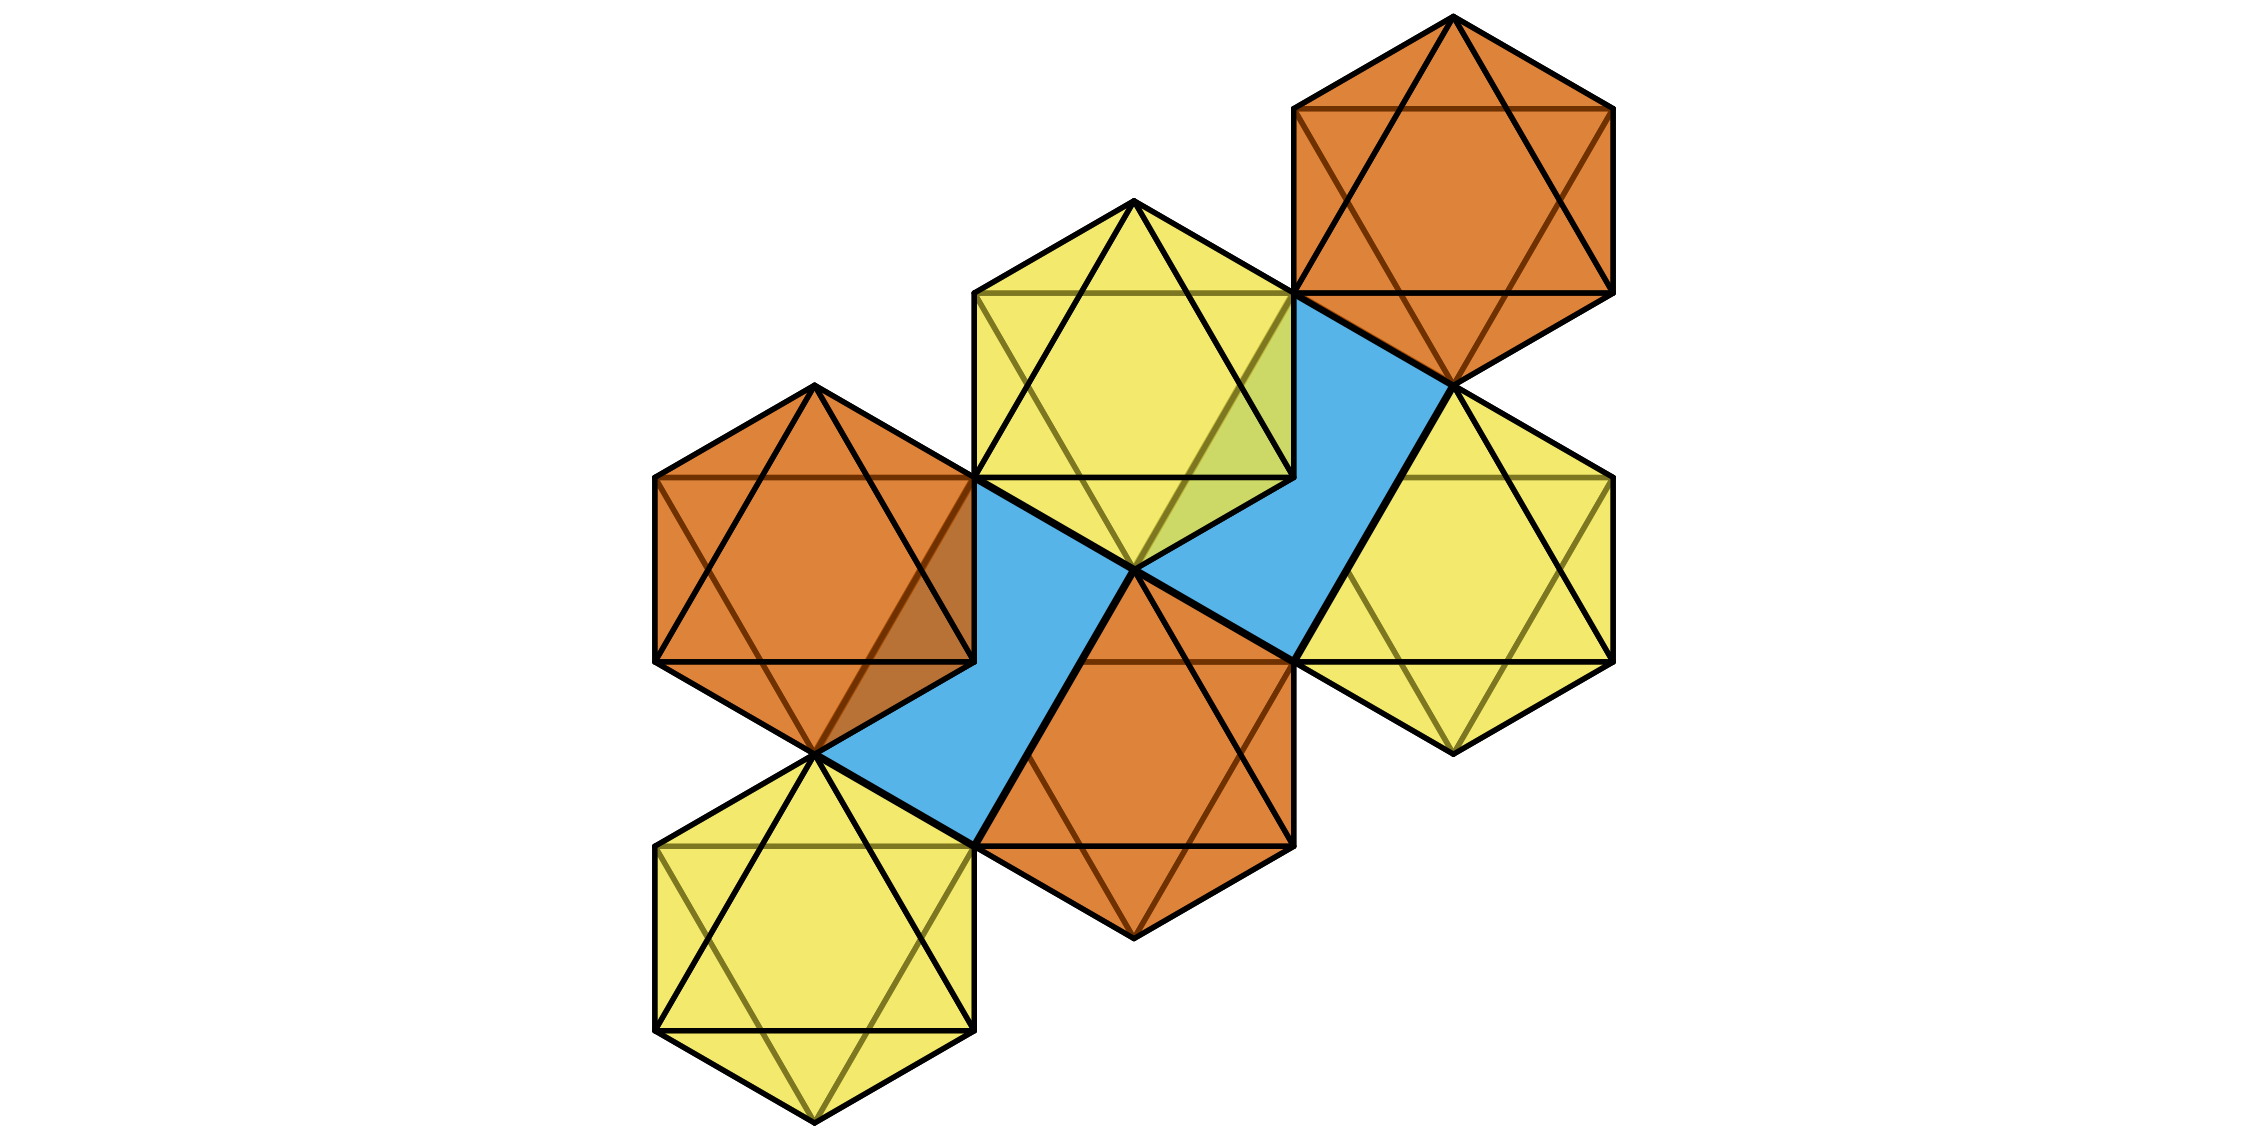
\includegraphics[width=\textwidth]{Figure 7.2.J}
\caption{The finite-difference mesh in 3D creates octahedrons with diamonds that reveal non-local dependency of checkerboard patterns}
\end{figure}
This finite-difference graph may form a closed shape with a specific Euler characteristic $\chi$. Since a Boolean random walk is a random process, the $\chi$ value of a finite-difference mesh changes randomly over time in a Boolean random walk. The assumption is that a macroparticle is a set of states that tend towards each other, and that such states have identical topological properties. For more on closed shapes regarding finite-difference meshes, see \textit{\S 7.8 Discrete Topology}.

\section{Directed Graphs}
A \textbf{directed graph}\index{directed graph} $G$ is a set of vertices $V$ connected by a set of directed edges, or arrows, $E$. The edge $(x,y)$ points from the tail $x$ to the head $y$. If $x$ directs to $y$, then $(x,y) = 1$. If $x$ does not direct to $y$, then $(x,y) = 0$. The edges $(x,y)$ and $(y,x)$ are now distinct and not necessarily equal.

\textbf{Edge contraction}\index{edge contraction} is a way that we may represent collections of states (or macrostates). By merging two vertices $\{u, v\}$ connected by an edge $(u, v)$ or $(v, u)$, a contracted vertex $w$ is formed containing all edges from both of the original vertices $\{u, v\}$. \textbf{Graph minors}\index{graph minor} are graphs formed by deleting edges, deleting vertices, and contracting edges:
\begin{figure}[H]
\centering
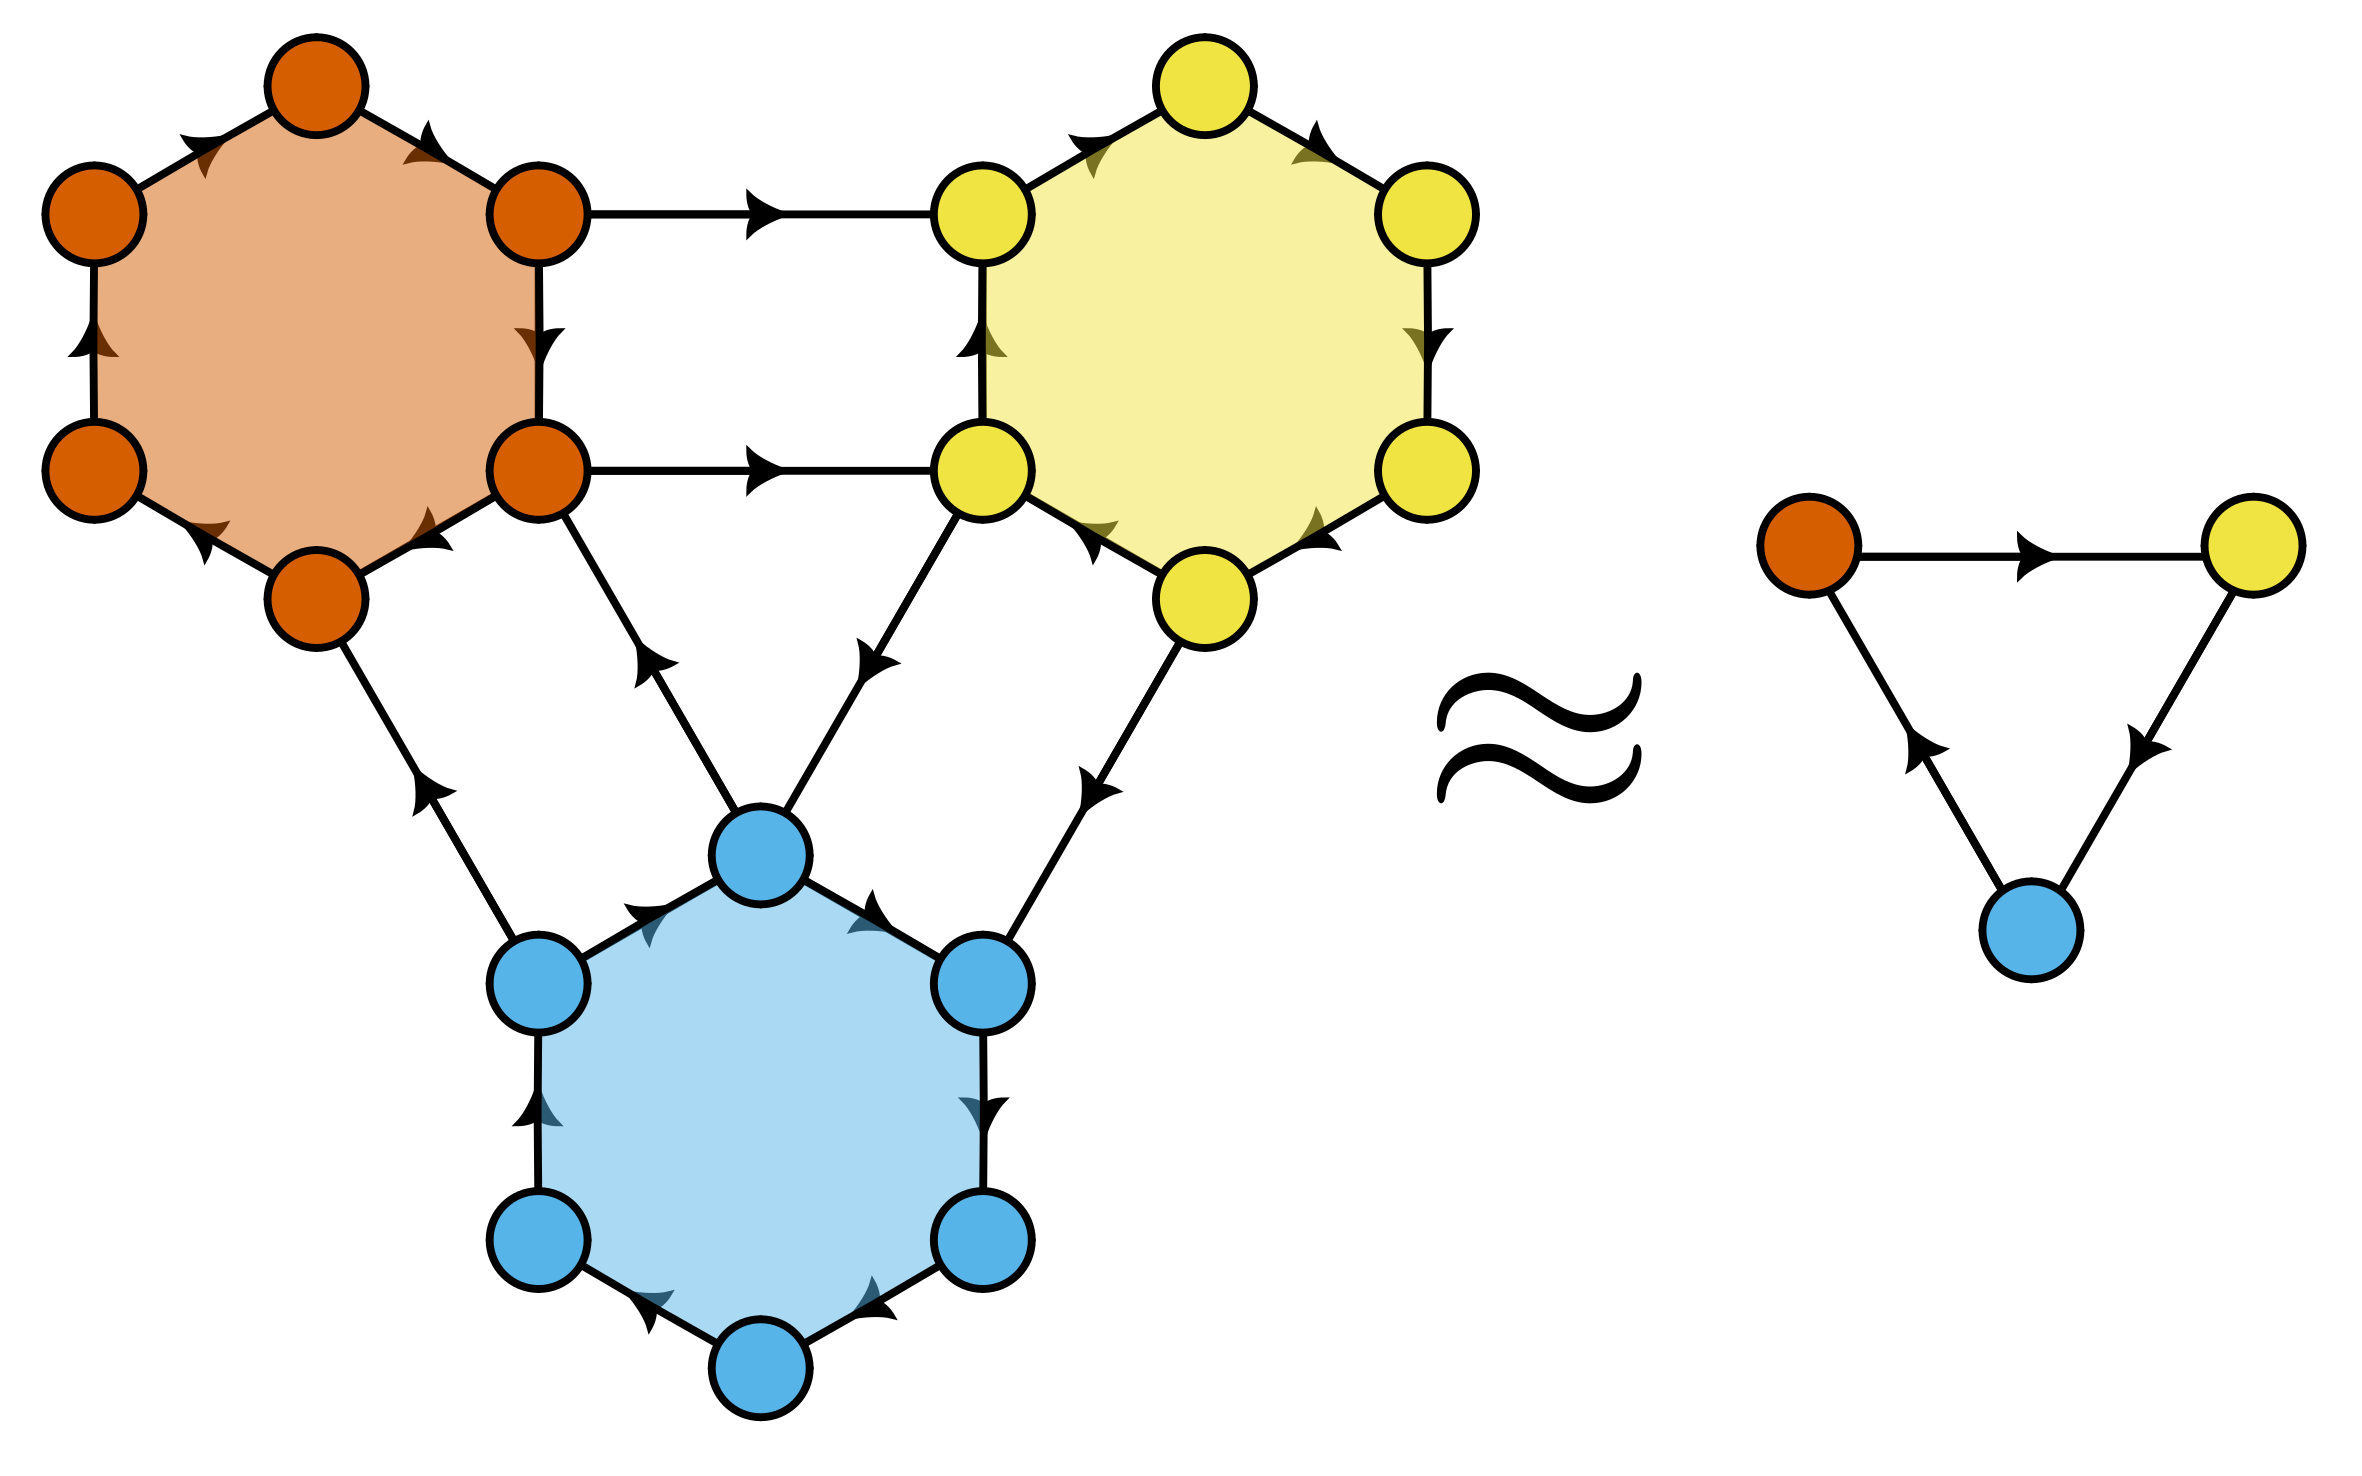
\includegraphics[width=\textwidth]{Figure 7.3.A}
\caption{The graph minor $g$ approximates the distribution of graph $G$}
\end{figure}
\noindent
The graph minor $g$ of the graph $G$ represents a reduced set of information about the original graph.

\section{Adjacency Matrix}
The \textbf{adjacency matrix}\index{adjacency matrix} $A$ of a graph $G$ represents the connectedness between vertices $V$. The adjacency matrix $A$ of an undirected graph $G$ is always a symmetric matrix because connections are mutual:
\begin{figure}[H]
\centering
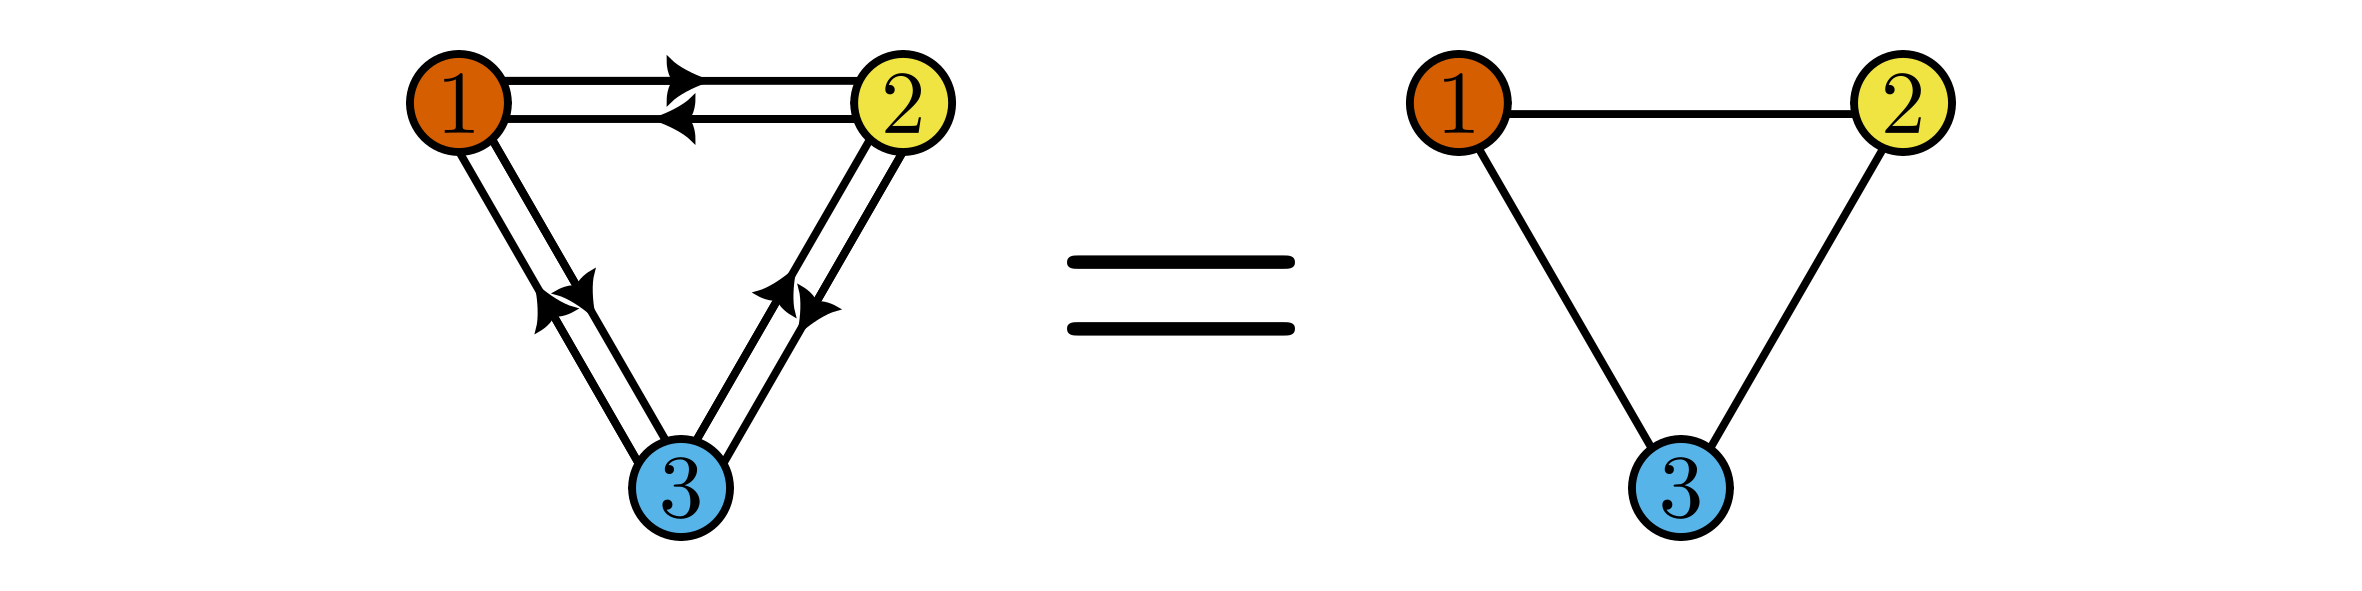
\includegraphics[width=\textwidth]{Figure 7.4.A}
\caption{Equal graph representations of an adjacency matrix}
\end{figure}
\noindent 
This graph has the following associated adjacency matrix:
$$ A = 
\begin{bmatrix}
0 & 1 & 1 \\
1 & 0 & 1 \\
1 & 1 & 0
\end{bmatrix}
= A^T $$
As a simple graph, it has no self-loops or self-adjacencies. Similar to graphs, we use the Boolean set $\mathbb B_\circ = \{0,1\}$ to represent connections between vertices.

The adjacency matrix $A$ of a directed graph $G$ may not be symmetric because connections may not be mutual:
\begin{figure}[H]
\centering
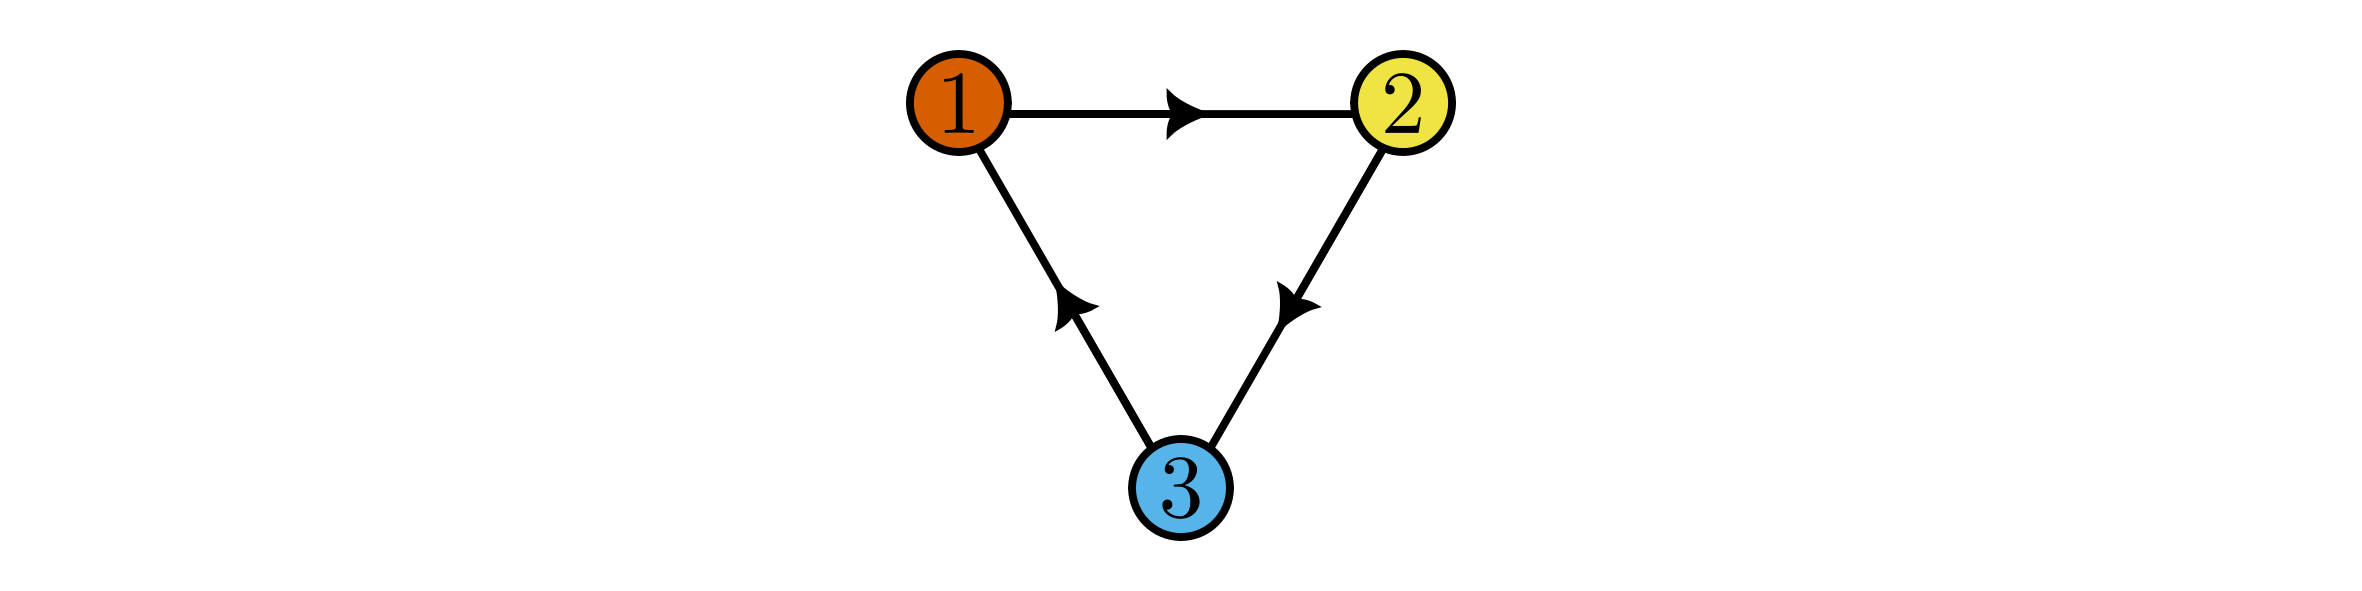
\includegraphics[width=\textwidth]{Figure 7.4.B}
\caption{A cyclical graph is not symmetric}
\end{figure} \noindent
It has the following adjacency matrix:
$$ A = 
\begin{bmatrix}
0 & 1 & 0 \\
0 & 0 & 1 \\
1 & 0 & 0
\end{bmatrix}
\neq A^T $$
Since this graph is not symmetric, its adjacency matrix $A$ does not equal its transpose $A^T$.

This Boolean matrix representation of graphs lends a few advantages. One advantage is that the matrix $A^n$ gives the number of $n$-length walks from state $\hat X_i$ to state $\hat X_j$. In the triangle cycle example, $A^n$ will only have a single $n$-length walk possible at any power of $n$:
\begin{figure}[H]
\centering
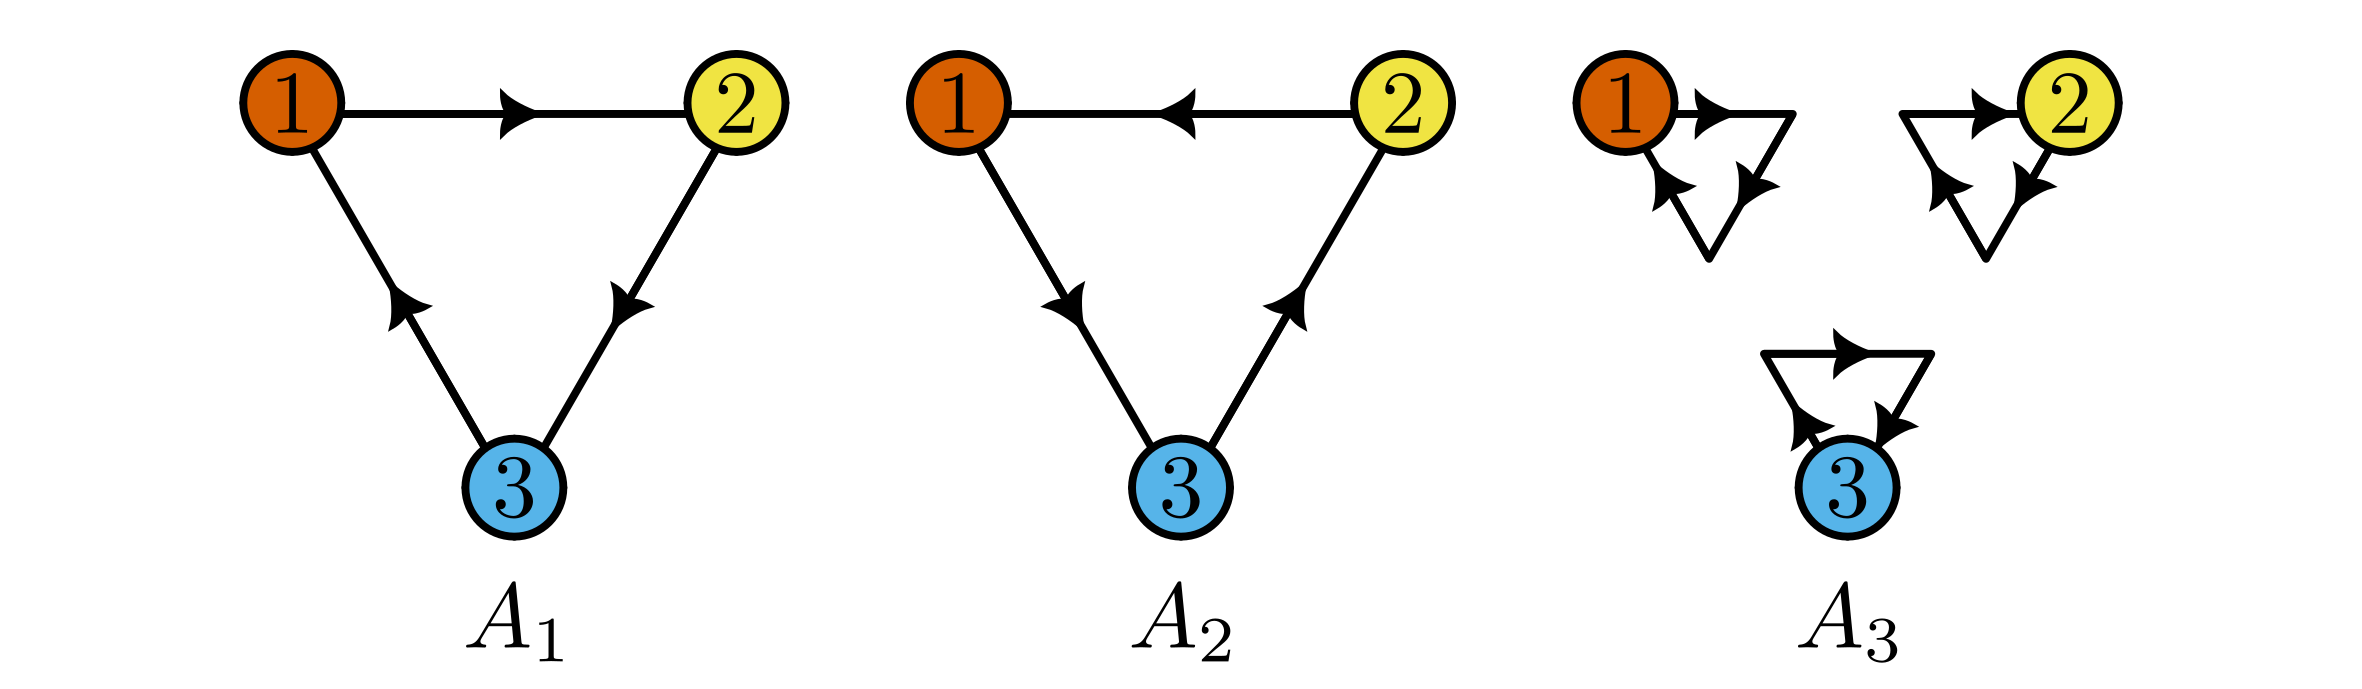
\includegraphics[width=\textwidth]{Figure 7.4.C}
\caption{Matrix powers of a cyclical permutation matrix}
\end{figure}
These are the following matrix representations of the graphs.
$$ A = 
\begin{bmatrix}
0 & 1 & 0 \\
0 & 0 & 1 \\
1 & 0 & 0
\end{bmatrix}
\quad
A^2 = 
\begin{bmatrix}
0 & 0 & 1 \\
1 & 0 & 0 \\
0 & 1 & 0
\end{bmatrix}
\quad
A^3 = 
\begin{bmatrix}
1 & 0 & 0 \\
0 & 1 & 0 \\
0 & 0 & 1
\end{bmatrix}
$$

Another advantage is that it is easier to tell if two graphs $G_1$ and $G_2$ are isomorphic, equal under some transformation. Two graphs are isomorphic if their vertices are permutations of each other. If $A_1$ is the adjacency matrix of graph $G_1$ and $A_2$ is the adjacency matrix of graph $G_2$, then $G_1$ and $G_2$ are isomorphic if and only if there exists some $Q$ such that:
$$Q A_1 Q^{-1} = A_2$$
in which $Q$ is a \textbf{permutation matrix}\index{permutation matrix} that rearranges the vertices of graph. It is worth noting that $Q^{-1} = Q^T$ because $Q$ is an orthonormal matrix. An \textbf{orthonormal matrix} is a matrix $Q$ in which the matrix multiplied by its transpose is the identity matrix: 
$$Q Q^T= Q^T Q = I$$

\section{Transition Matrix}
A \textbf{transition matrix}\index{transition matrix}, or \textbf{stochastic matrix}\index{stochastic matrix}, $P$ is an adjacency matrix $A$ with a probability measure applied to it. If $P$ is a right stochastic matrix such that:
$$\sum\limits_{j=1}^\theta P_{(i, j)} = 1$$
for all rows $i \in 1,...,\theta$ in which $\theta$ is the total number of states, then:
$$P = A \mu_R = \mu_L A$$
in which $\mu_R$ is the right measure matrix and $\mu_L$ is the left measure matrix. We may observe the relation that $\mu_R = A^{-1}\mu_L A$. The measure matrices share eigenvalues $\lambda_1,...,\lambda_\theta$ but not eigenvectors. If the adjacency matrix $A$ is not invertible, then replace $A^{-1}$ with the Moore-Penrose pseudo-inverse $A^+$.

The rationale for preferring right measure matrices for right stochastic matrices is due to the simplicity of calculating \textbf{normalized eigenvector centrality}\index{normalized eigenvector centrality}, also known Google PageRank. The PageRank formula is given by:
$$A^{-1} C D_C^{-1} A v = v$$
in which $v$ is the score of row in the stochastic matrix $P = C D_C^{-1}$. If $C$ is a matrix counting the number of citations, then $D_C^{-1}$ is a diagonal matrix that normalizes the rows of $C$ to sum to $1$. It is worth noting that $v$ also sums to $1$, and might be interpreted as the distribution of attention.

The normalized eigenvector centrality formula for $v$ can be simplified as:
$$A^{-1} P A v = v $$
$$A^{-1} A \mu_R A v = v$$
$$\mu_R A v = v$$
The PageRank formula is the eigenvector of $\mu_R A$ with eigenvalue $1$, and $\mu_R A$ is the reverse composition of $P = A \mu_R$. It is more useful to consider the \textit{absolute value} of the eigenvector squared $|v|^2$ since it is calculable for $2$-periodic stochastic matrices with complex eigenvalues.

A transition matrix $P$ that is \textit{weakly mixing} has a limiting transition matrix $\Lambda$.\footnote{Strongly mixing is more restrictive and implies weakly mixing.} A transition matrix that is weakly mixing is ergodic, meaning it has only one communication class and only one eigenvalue of unit magnitude $|\lambda| = 1$. For any weakly mixing transition matrix $P$, it approaches the limiting distribution $\Lambda$ as time $t$ approaches $\infty$:
$$\Lambda = \lim\limits_{t \rightarrow \infty} P^t$$
If transition matrix $P$ is ergodic, this limiting transition matrix $\Lambda$ distributes probability within each row until it reaches the stationary distribution. A Boolean mechanical system governed by a Boolean random walk does not have a limiting transition matrix because it is not $1$-periodic, therefore not ergodic. This is because it has an eigenvalue of $\lambda = -1$, meaning it is a $2$-periodic system. A $2$-periodic transition matrix has two classes of states that will never mix: even and odd states. 

Consider two transition matrices $A$ and $B$:
$$ 
A = 
\begin{bmatrix}
1 & 0 \\
0 & 1
\end{bmatrix}
\quad \quad
B = 
\begin{bmatrix}
0.5 & 0.5 \\
0.5 & 0.5
\end{bmatrix}
$$
The matrix $A$ will never reach some limiting distribution matrix $\Lambda$ while the matrix $B$ is its own limiting distribution.

When a transition matrix's mixing slows down dramatically, it is because two or more communication classes resist the transfer of probability. We might say that they communicate weakly:
\begin{figure}[H]
\centering
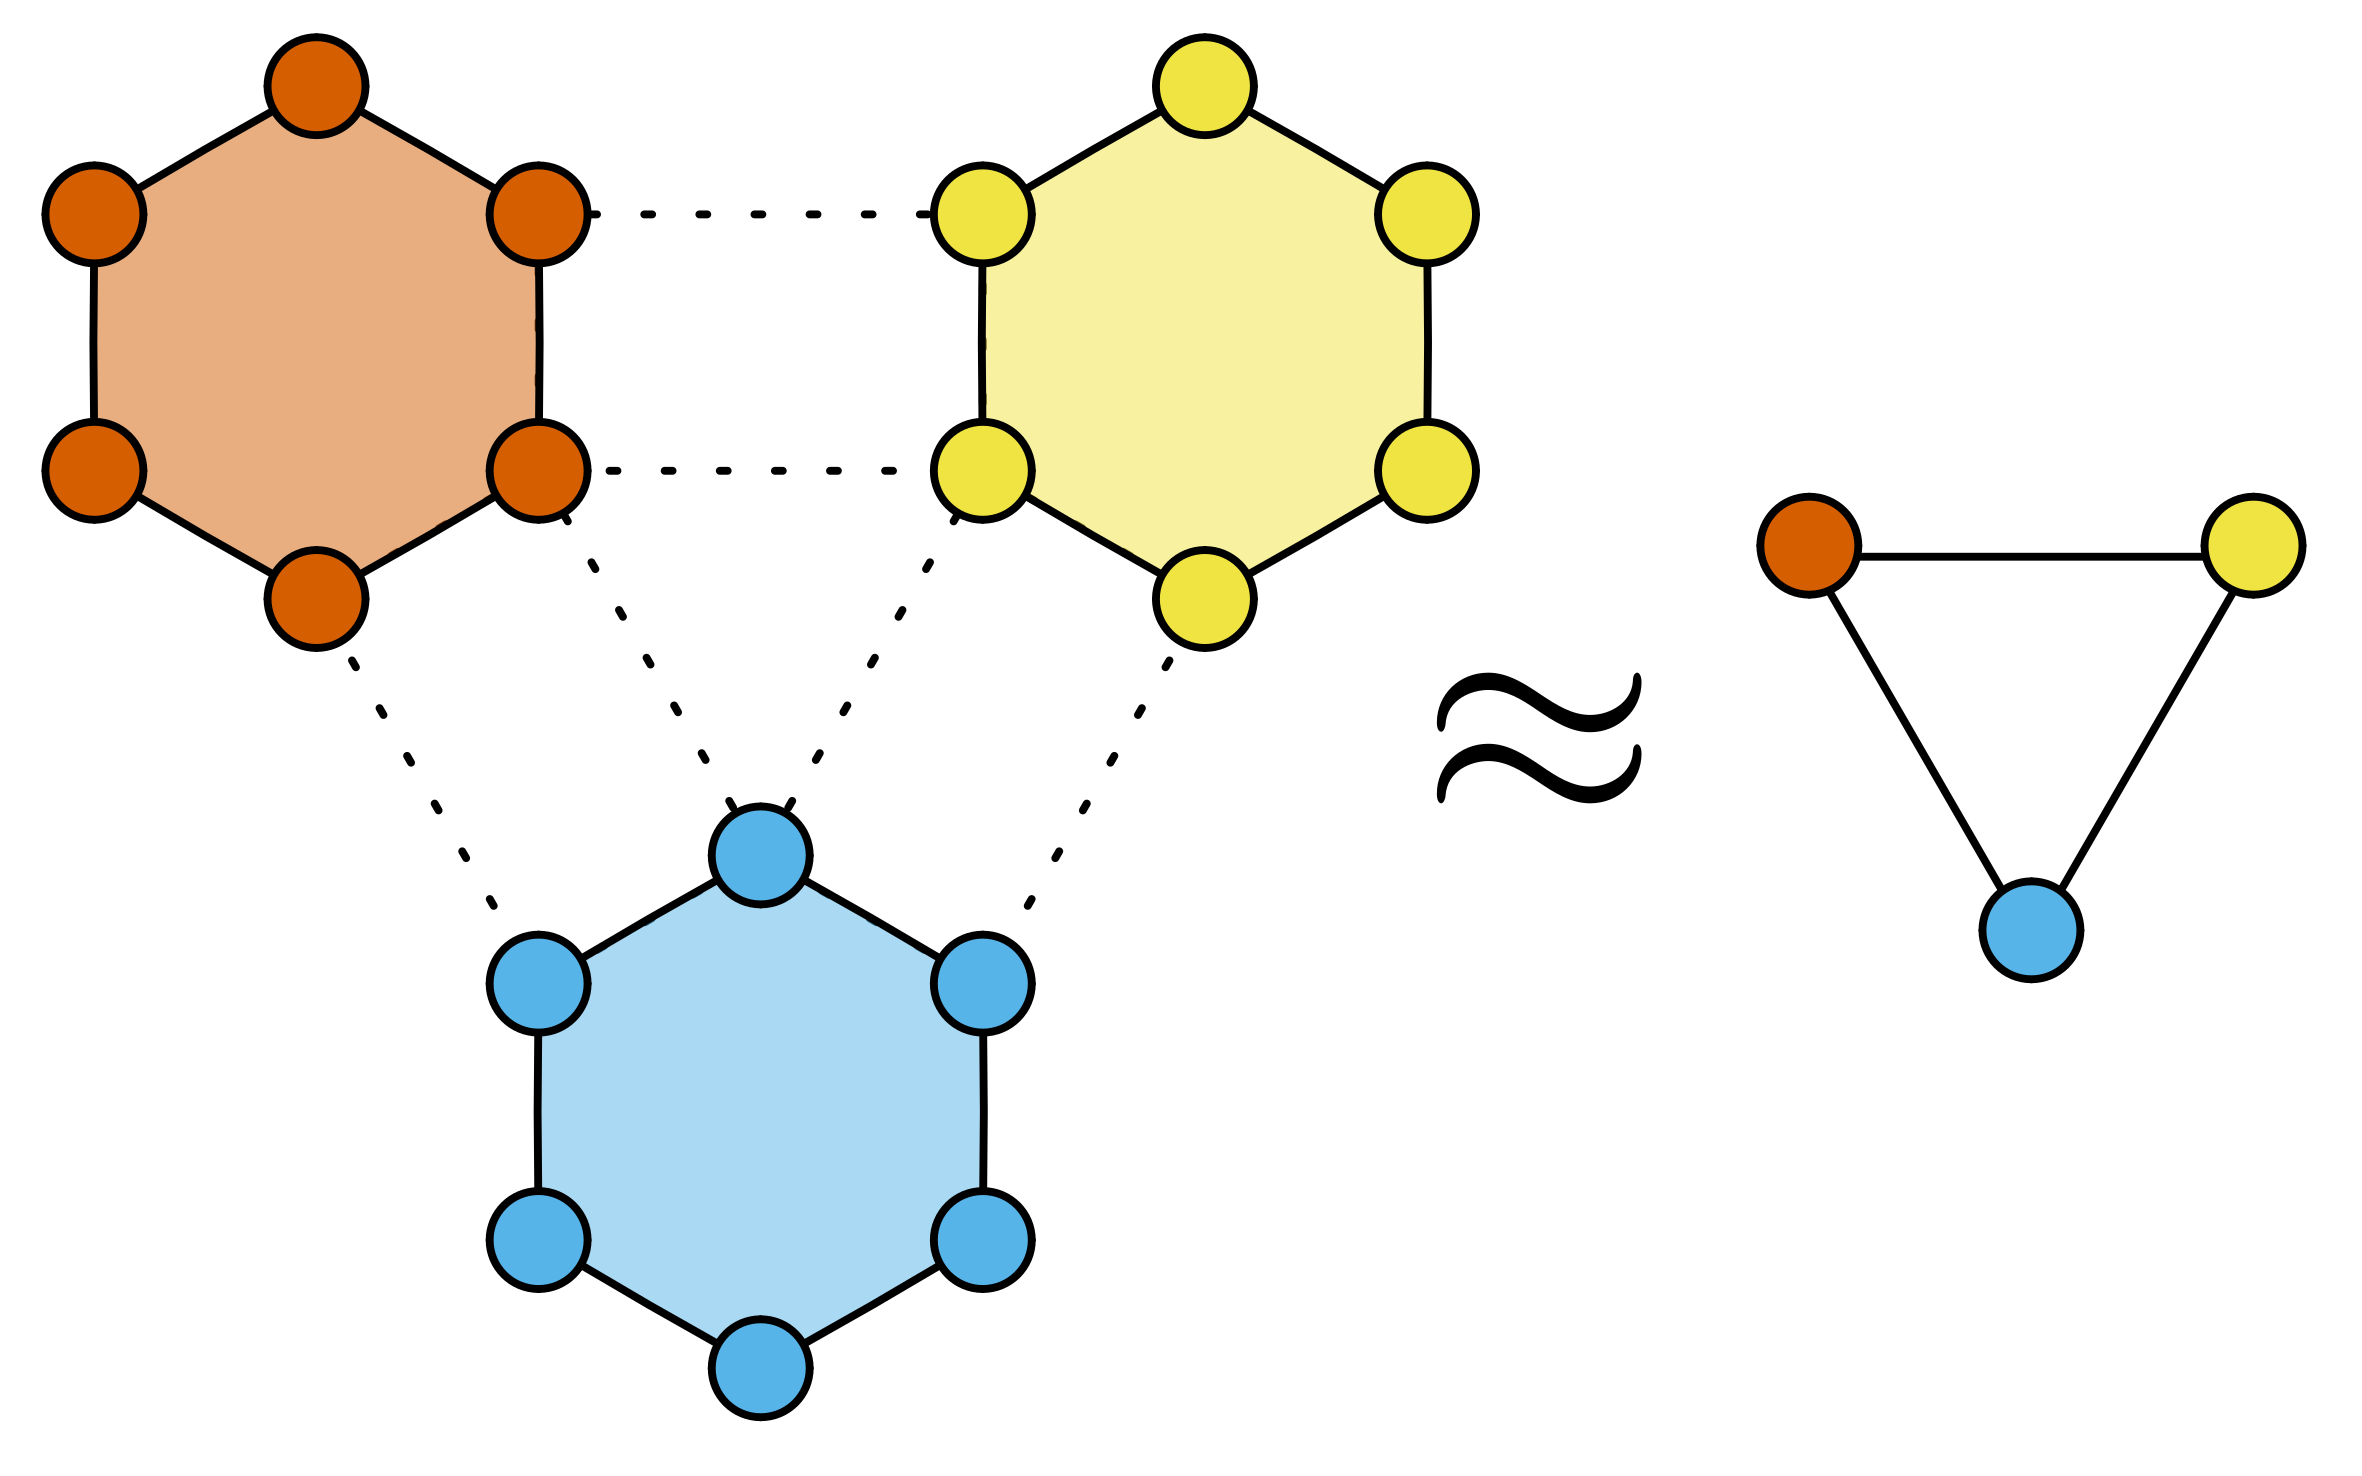
\includegraphics[width=\textwidth]{Figure 7.5.A}
\caption{States that communicate strongly become indistinguishable}
\end{figure} \noindent 
The transition matrix of this graph is similar to a reducible transition matrix with three communication classes. However, there is a very small transition probability between the three ``classes''. For more on methods to classify states with similar future distributions, see \textit{\S Appendix D: Class Stochastic Matrices}

The \textbf{spectral gap}\index{spectral gap} $\xi$ of a transition matrix $P$ measures how long it takes for a stochastic process to reach equilibrium. It is often defined either as the absolute difference between the two largest eigenvalues:
$$\xi = |\lambda_1| - |\lambda_2|$$
The standard convention is to order our eigenvalues in decreasing order of magnitude such that:
$$|\lambda_1| \leq |\lambda_2| \leq ... \leq |\lambda_\theta|$$
For a Boolean random walk, we have a zero spectral gap:
$$\xi = |\lambda_1 - \lambda_2| = |1| - |-1| = 0$$
because the odd states and even states never mixes completely.

A definition spectral gap that adjusts periodic systems is to consider the largest eigenvalue with magnitude between zero and one:
$$\xi = |\lambda_1| - |\lambda_{\textnormal{max}}|, \quad \lambda_{\textnormal{max}} = \max_{i\in 1,...,\theta} (0 < |\lambda_i| < 1)$$
This removes the awkward case of zero spectral gaps when we have multiple unit magnitude eigenvalues. If the point of a spectral gap is to represent how long it takes to reach maximal mixing, then this is a better definition. We might say the inverse of the spectral gap $\xi^{-1}$ roughly indicates the time when the last edge contractions happen.\footnote{This intuition is correct as the initial definition of spectral gap gives an inverse spectral gap of $\xi = \infty$ for Boolean random walks due to non-mixing of even and odd states.}

The alternative definition for spectral gap is the smallest eigenvalue greater than $0$:
$$\xi = \min_{i\in 1,...,\theta} (\lambda_i \ge 0)$$
stated as $\lambda_\theta$. For a Boolean random walk, it gives $\xi = \lambda_\theta \approx 1$ due often having \textit{at least one pair} of states that \textit{strongly communicate}. This definition is not common and should not be taken as the most important part of the mixing rate of a Boolean random walk. We might say the inverse spectral gap $\xi^{-1}$ roughly indicates the time when the first edge contractions happen.

If $P$ is a matrix, then $P = \Phi \Lambda \Phi^{-1}$ is called the \textbf{eigendecomposition}\index{eigendecomposition} of the matrix. Powers of a transition matrix $P$ have the following relationship:
$$P^t = \Phi \Lambda^t \Phi^{-1}$$
in which $\Lambda$ is a diagonal matrix with eigenvalues $\lambda_1,...,\lambda_\theta$ and $\Phi$ is a matrix in which each column is an eigenvector $\phi_1,...,\phi_\theta$. We will define $\Phi = \phi_1,...,\phi_\theta$ as the set of column eigenvectors with unit magnitude. An eigenvector $\phi$ is unit magnitude if $\phi \cdot \phi^* = 1$, in which $\phi^*$ is the complex conjugate of $\phi$. An alternative definition of unit magnitude $\phi$ is that $|\phi|^2 = 1$. This is important because a Boolean random walk may have complex eigenvalues, and therefore complex eigenvectors.

A transition matrix mixes quite slowly if many eigenvalues are quite close to magnitude $1$, and different parts mix at different rates according to the spectrum. The eigenvalues of any $n \times n$ stochastic transition matrix are bounded by Karpelevich regions:
\begin{figure}[H]
\centering
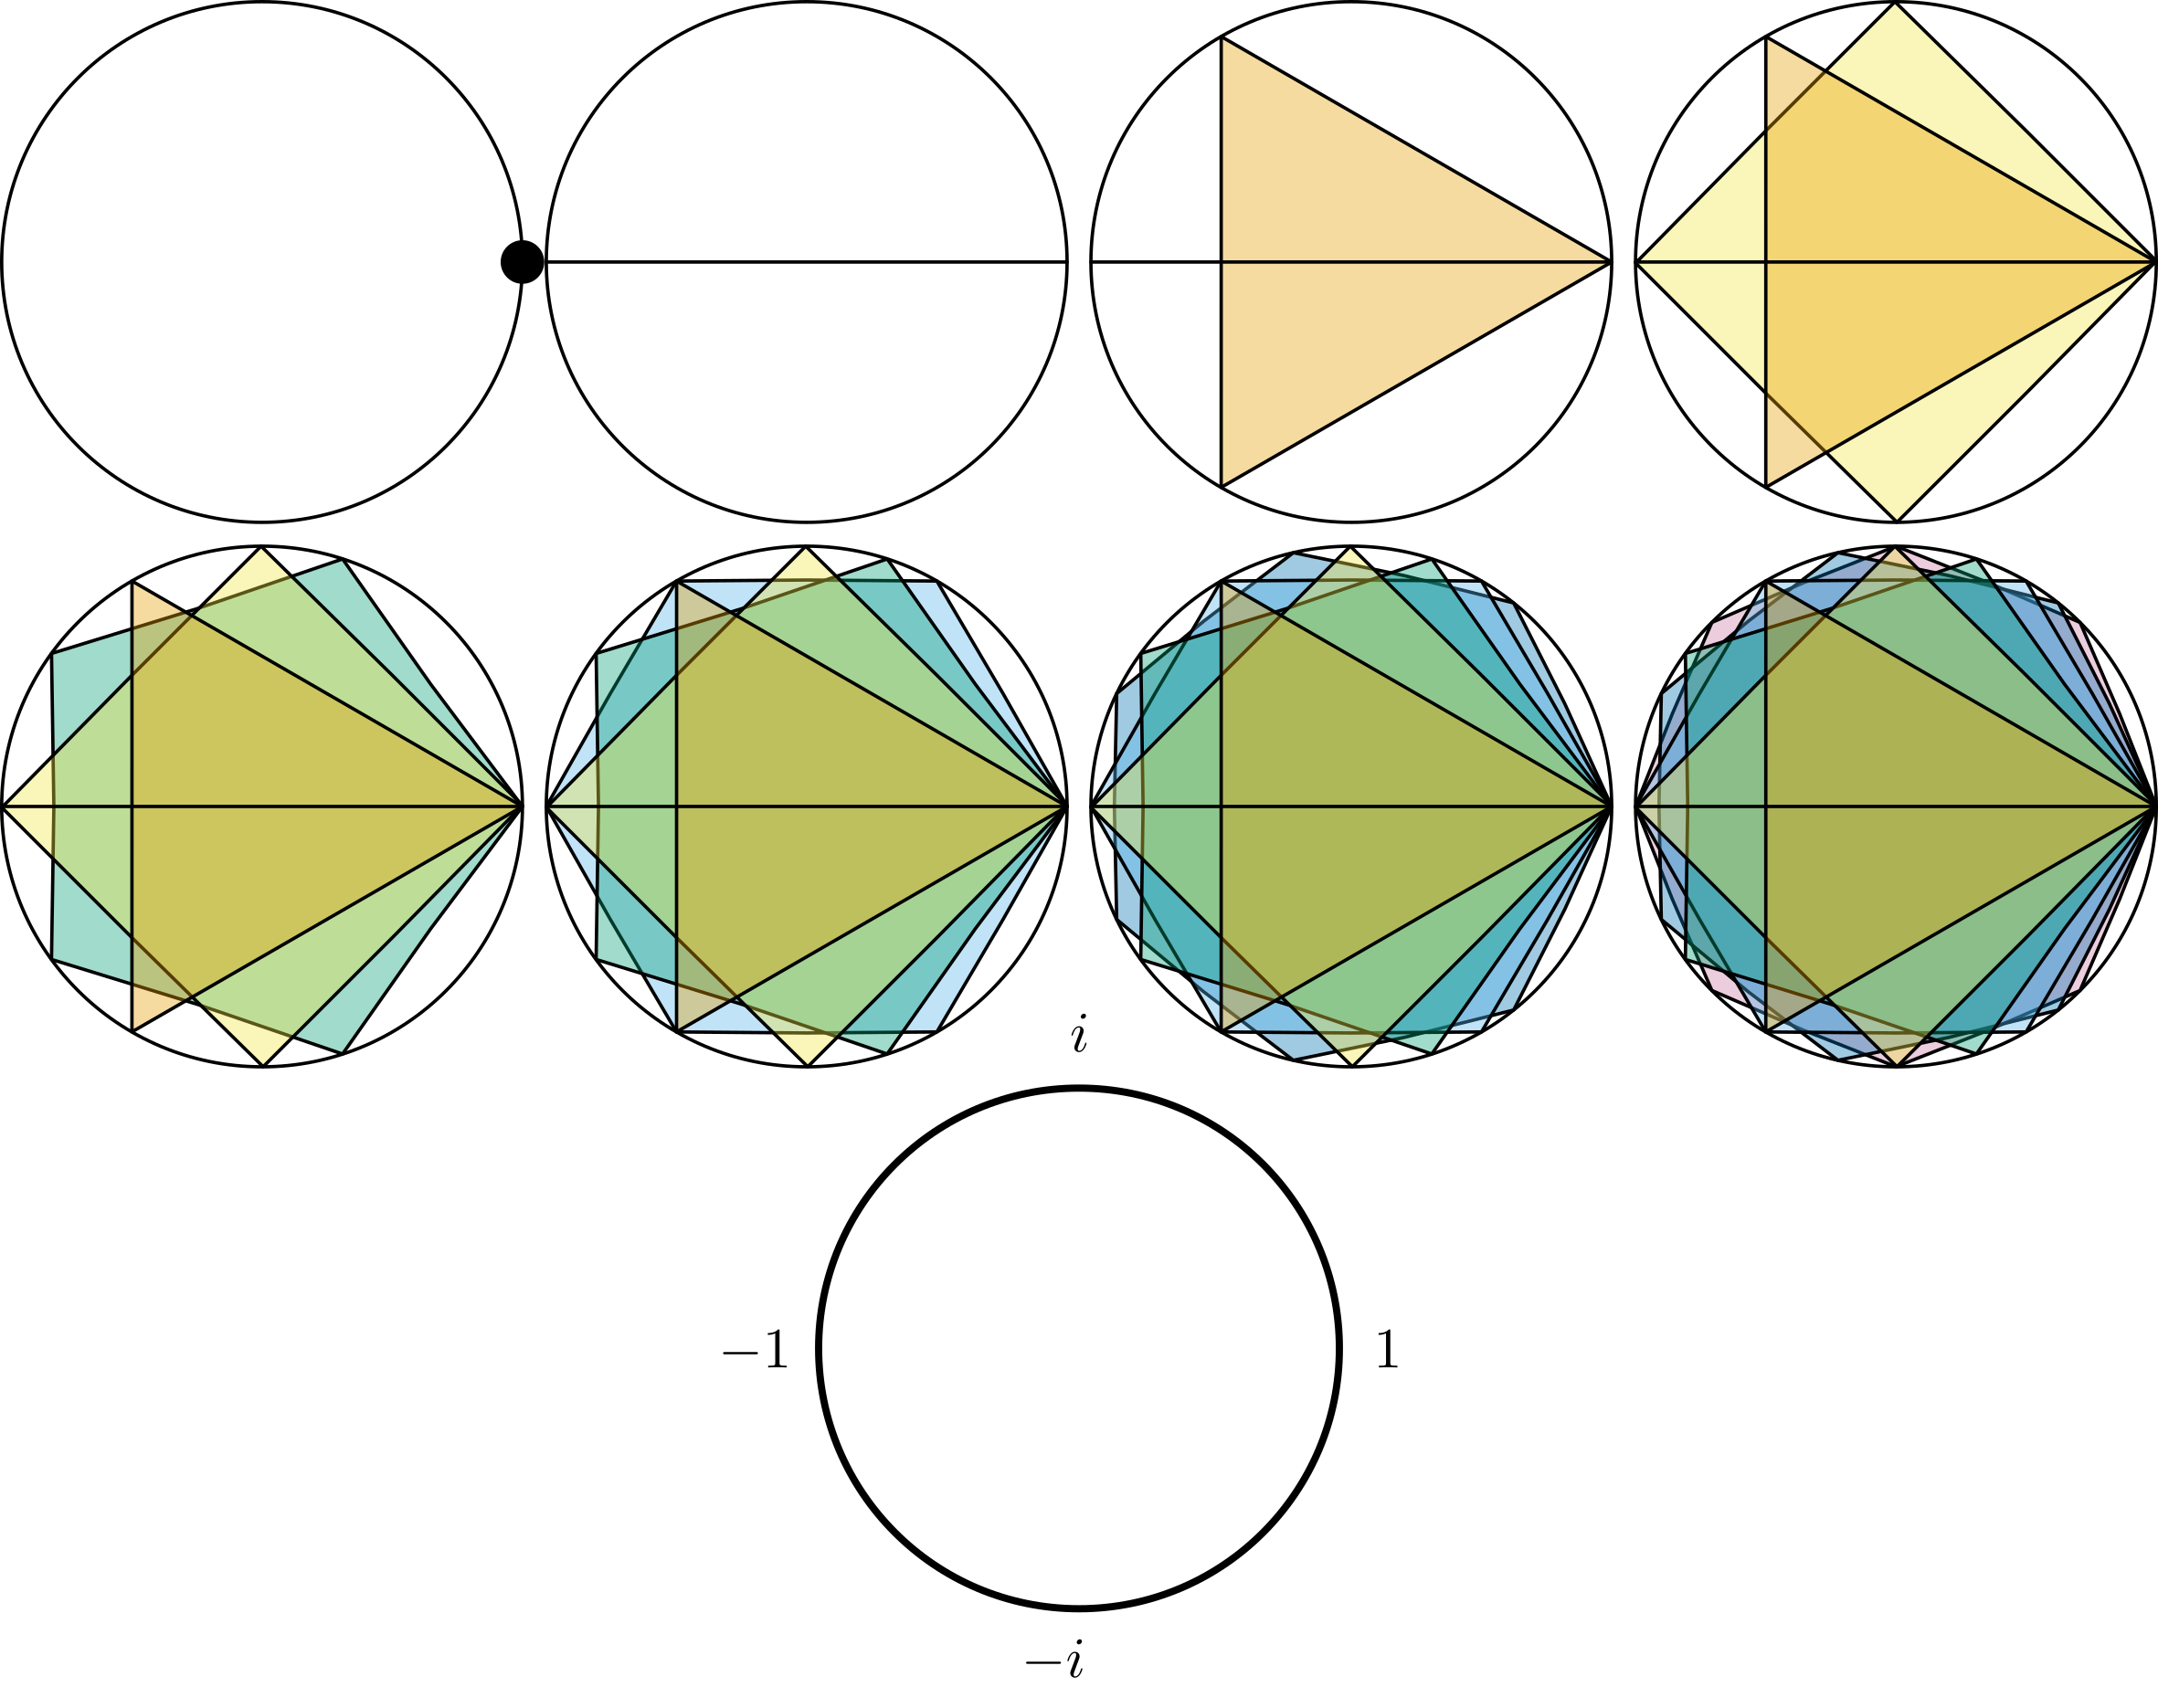
\includegraphics[width=\textwidth]{Figure 7.5.B}
\caption{Karpelevich region approximations with polygons}
\end{figure} \noindent 
\noindent % Karpelevich regions for 3x3, 4x4, and 5x5 stochastic matrices
Karpelevich regions are a subset of the complex disc. This diagram does not accurately capture the size of each Karpelevich region. True Karpelevich regions extend slightly further than the union of polygons, curving gently instead of bending sharply in each concave.

Each eigenvector represents a harmonic eigenstate $\hat A$, or normal mode, of the system. We use $A$ and $a$ to refer to a harmonic eigenstate as derived from Greek $\alpha \rho \mu o \nu \iota \kappa \acute o \varsigma$ (harmonic).\footnote{A position eigenstate is to a momentum eigenstate as a configuration eigenstate is to a harmonic eigenstate. It is appropriate to define position for a single random walker, but it is not sensible to define position for Boolean random walks.} Since each eigenvector is linearly independent and may be represented as a normal mode (i.e. a harmonic function) as a linear combination of states $\hat X_1,...,\hat X_\theta$, then $\ln(\lambda) = \eta$ refers to the eigenvalues of some damped harmonic oscillator's differential equation.

Note that small magnitudes for $\lambda_i$ refers to an eigenstate $\hat A_i$ whose contribution dampens quickly In contrast, large magnitudes for $\lambda_i$ refer to the larger eigenstates, or normal modes with strong sustain. This is relevant to the heat equation as discussed in \textit{\S 8.4 Diffusion and Heat Equation} since high temperature differences in a fluid are smooth out faster while low temperature differences smooth out slower. 

We will call these constructed harmonic eigenstates as $\hat A$. For example, suppose we have a simple random walk on a 1D lattice of length $5$. The stochastic matrix $P$ is the following:
$$P = 
\begin{bmatrix}
0 & 1 & 0 & 0 & 0 \\
\frac{1}{2} & 0 & \frac{1}{2} & 0 & 0 \\
0 & \frac{1}{2} & 0 & \frac{1}{2} & 0 \\
0 & 0 & \frac{1}{2} & 0 & \frac{1}{2} \\
0 & 0 & 0 & 1 & 0
\end{bmatrix}
$$
It has an eigendecomposition $P = \Phi \Lambda \Phi^{-1}$ in which:
\[ \Phi = \frac{1}{\sqrt 5}
\begin{bmatrix}
1 & 1 & -1 & -1 & 1 \\
1 & -1 & \frac{1}{\sqrt 2} & -\frac{1}{\sqrt 2} & 0 \\
1 & 1 & 0 & 0 & -1 \\
1 & -1 & -\frac{1}{\sqrt 2} & \frac{1}{\sqrt 2} & 0 \\
1 & 1 & 1 & 1 & 1
\end{bmatrix}\]
\[
\Lambda = \begin{bmatrix}
1 & 0 & 0 & 0 & 0 \\
0 & -1 & 0 & 0 & 0 \\
0 & 0 & -\frac{1}{\sqrt 2} & 0 & 0 \\
0 & 0 & 0 & \frac{1}{\sqrt 2} & 0 \\
0 & 0 & 0 & 0 & 0
\end{bmatrix}
\]
Then the harmonic eigenstate $\hat A_2$ for a simple random walk in a bounded lattice is necessarily the checkerboard state.
\begin{figure}[H]
\centering
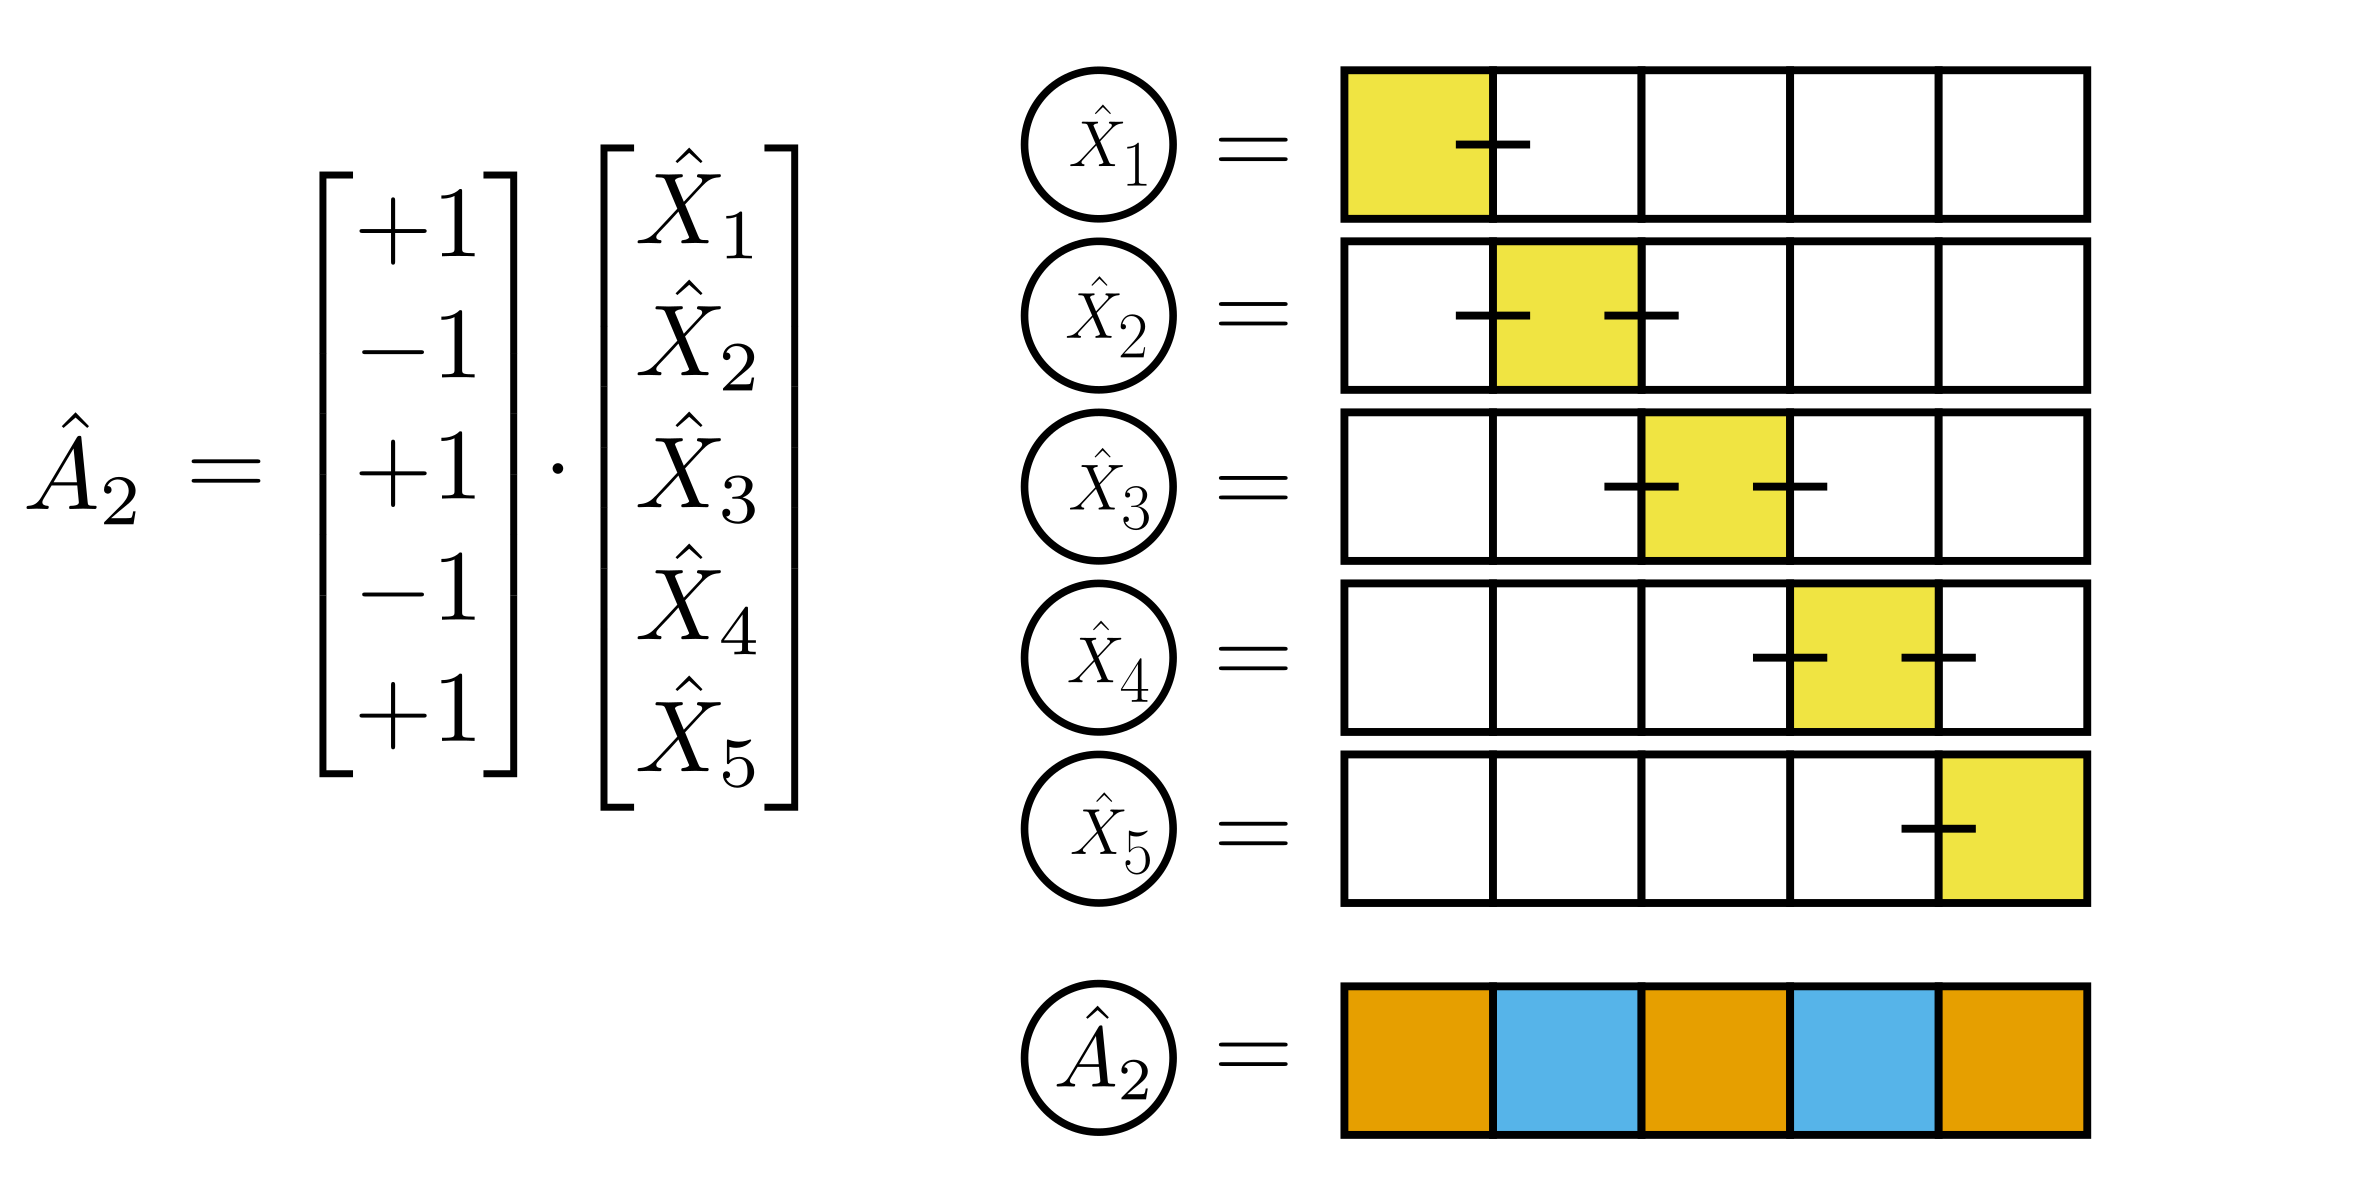
\includegraphics[width=\textwidth]{Figure 7.5.C}
\end{figure} \noindent 
since it corresponds to eigenvalue $\lambda_2 = -1$. Since matrix powers of $P$ are given by $P = \Phi \Lambda^t \Phi^{-1}$, we interpret the eigenvalue $\lambda_2^t = (-1)^t$ as oscillating the normal mode. Other normal modes are much stranger, especially those with complex eigenvalues.

Some the the interesting properties of Boolean random walk eigenvalues are given like so:
$$\delta = \sum\limits_{i=1}^\theta \textnormal{Re}(\lambda_i) = 0$$
$$\chi = \sum\limits_{i=1}^\theta \textnormal{Im}(\lambda_i) = 0$$
$$\delta + \chi = 0$$
Since $P$ is a real matrix and complex eigenvalues come in conjugate pairs, then the imaginary portion of each complex eigenvalue $\lambda$ cancels out with its conjugate $\lambda^*$. The fact that the real portion of eigenvalues cancel out with each other is still a mystery. There must be some fundamental reason that requires further research involving the fact that a random walk is $2$-periodic. Other interesting properties are that:
$$\textnormal{det}(e^P) = e^{\textnormal{tr}(P)} = 1$$
This is property is derived regarding the fact that a Boolean random walk stochastic matrix has a trace of 0, and it is computationally 0 for approximations.

Each eigenvalue $\lambda_i$ can be decomposed into its magnitude $\mu_i$ and frequency $\omega_i$ such that:
$$\lambda_i = \mu_i e^{\omega_i}, \quad \mu_i = |\lambda_i|, \omega_i = \ln(\lambda_i) - \ln(\mu_i)$$
This relates $\mu$ to exponential decay and $\omega_i$ to rotation about the unit circle. The progression of harmonic eigenstate magnitudes may be visualized using an exponential decay cone:
\begin{figure}[H]
\centering
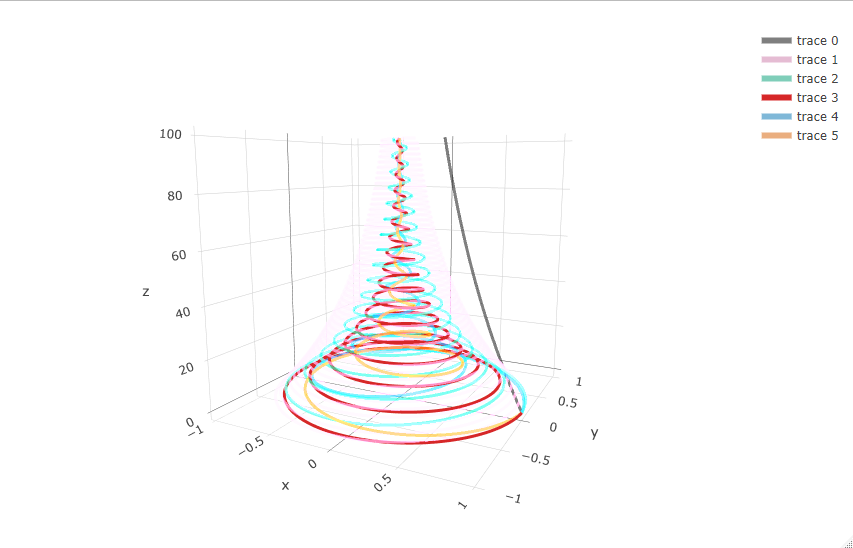
\includegraphics[width=\textwidth]{Figure 7.5.D}
\caption{An eigenvalue spiral of decaying eigenvalues}
\end{figure}
\noindent It helps to remember the interpretation for $\lambda_2 = -1$ is that the imaginary number $i = \sqrt{-1}$, therefore by convention rotating counter-clockwise.

\section{Flip Graphs and Bit Flips}
A \textbf{flip graph}\index{flip graph} is a graph $G$ whose edges link vertices that represent combinatorial objects, and each edge represents a transition from one object to another using a flip operation:
\begin{figure}[H]
\centering
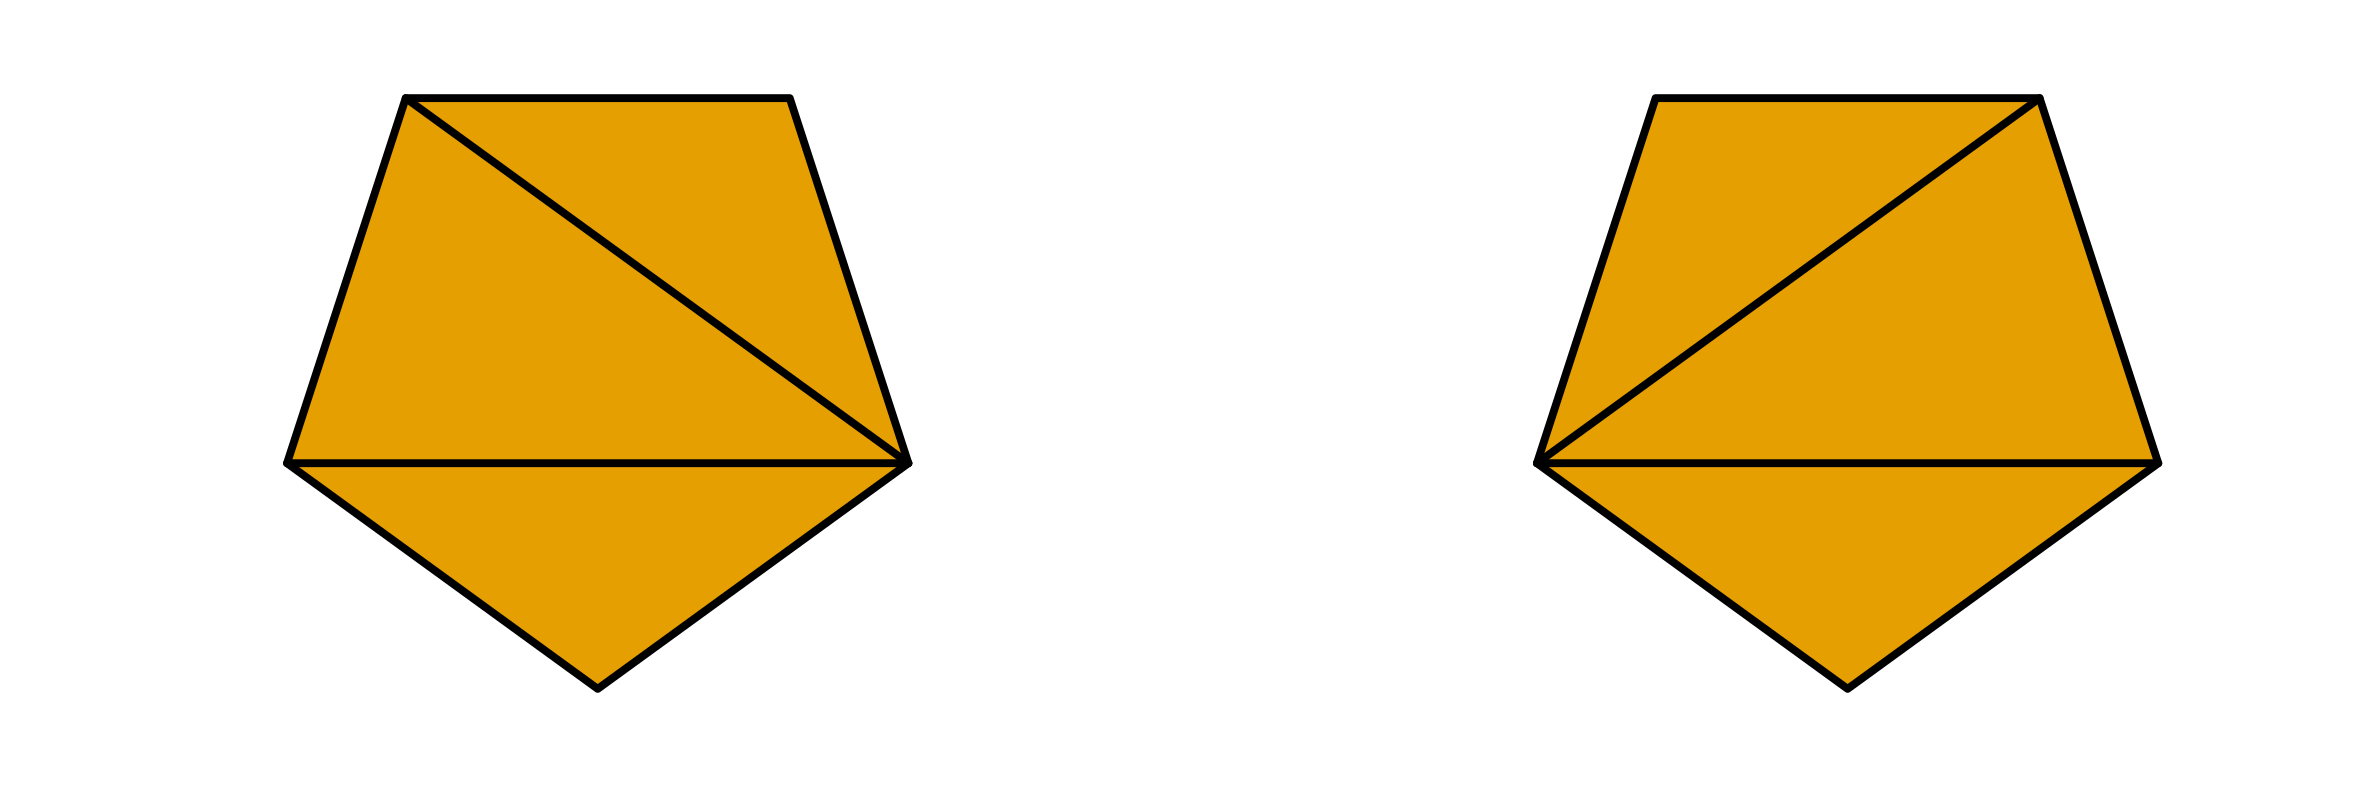
\includegraphics[width=\textwidth]{Figure 7.6.A}
\caption{Two adjacent states in the flip graph of a pentagon}
\end{figure}
\noindent 
Flip graphs commonly refer to triangulations, but we may assume the alternative definition for rectangular lattices.
\begin{figure}[H]
\centering
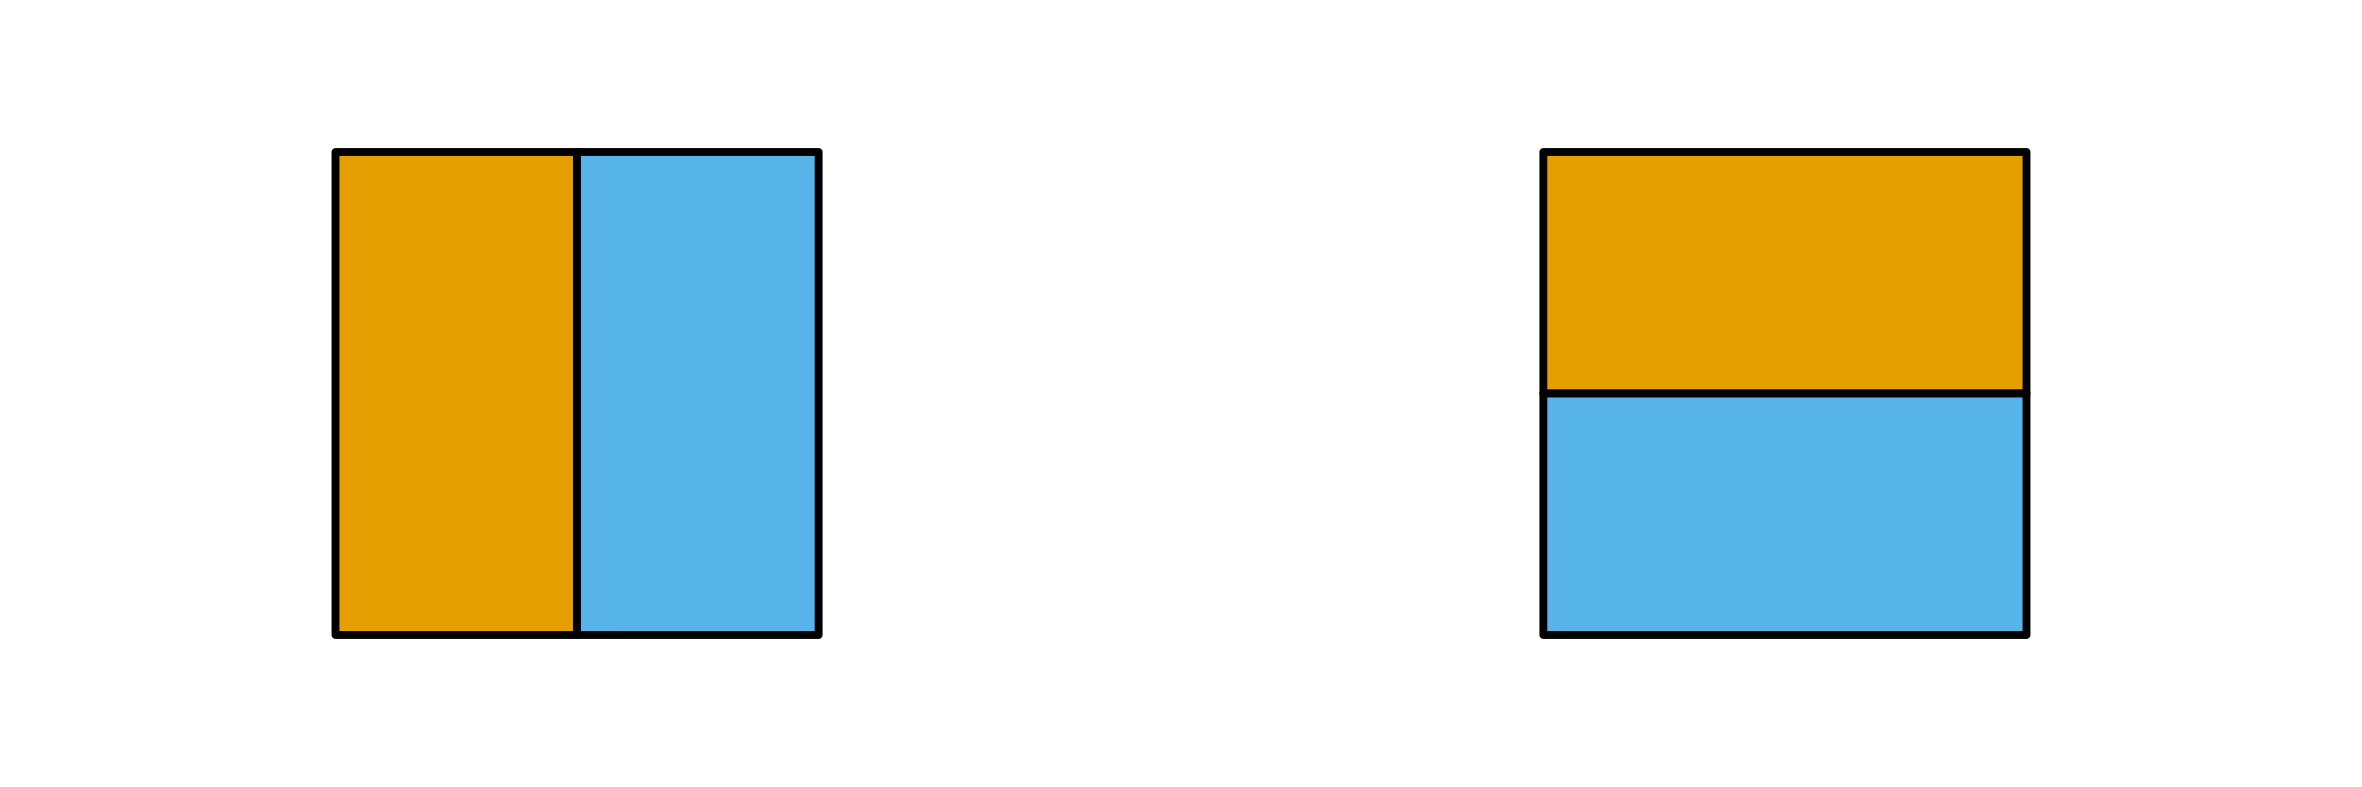
\includegraphics[width=\textwidth]{Figure 7.6.B}
\caption{Two adjacent states domino tilings}
\end{figure}
The flips of domino tilings have interesting properties, especially when a domino tiling can represent a specific Boolean random walk transition.

Flip graphs are additionally relevant to Boolean mechanics because a Boolean random walk exchanging a particle and an antiparticle corresponds to a bit flip in a Boolean computer:
\begin{figure}[H]
\centering
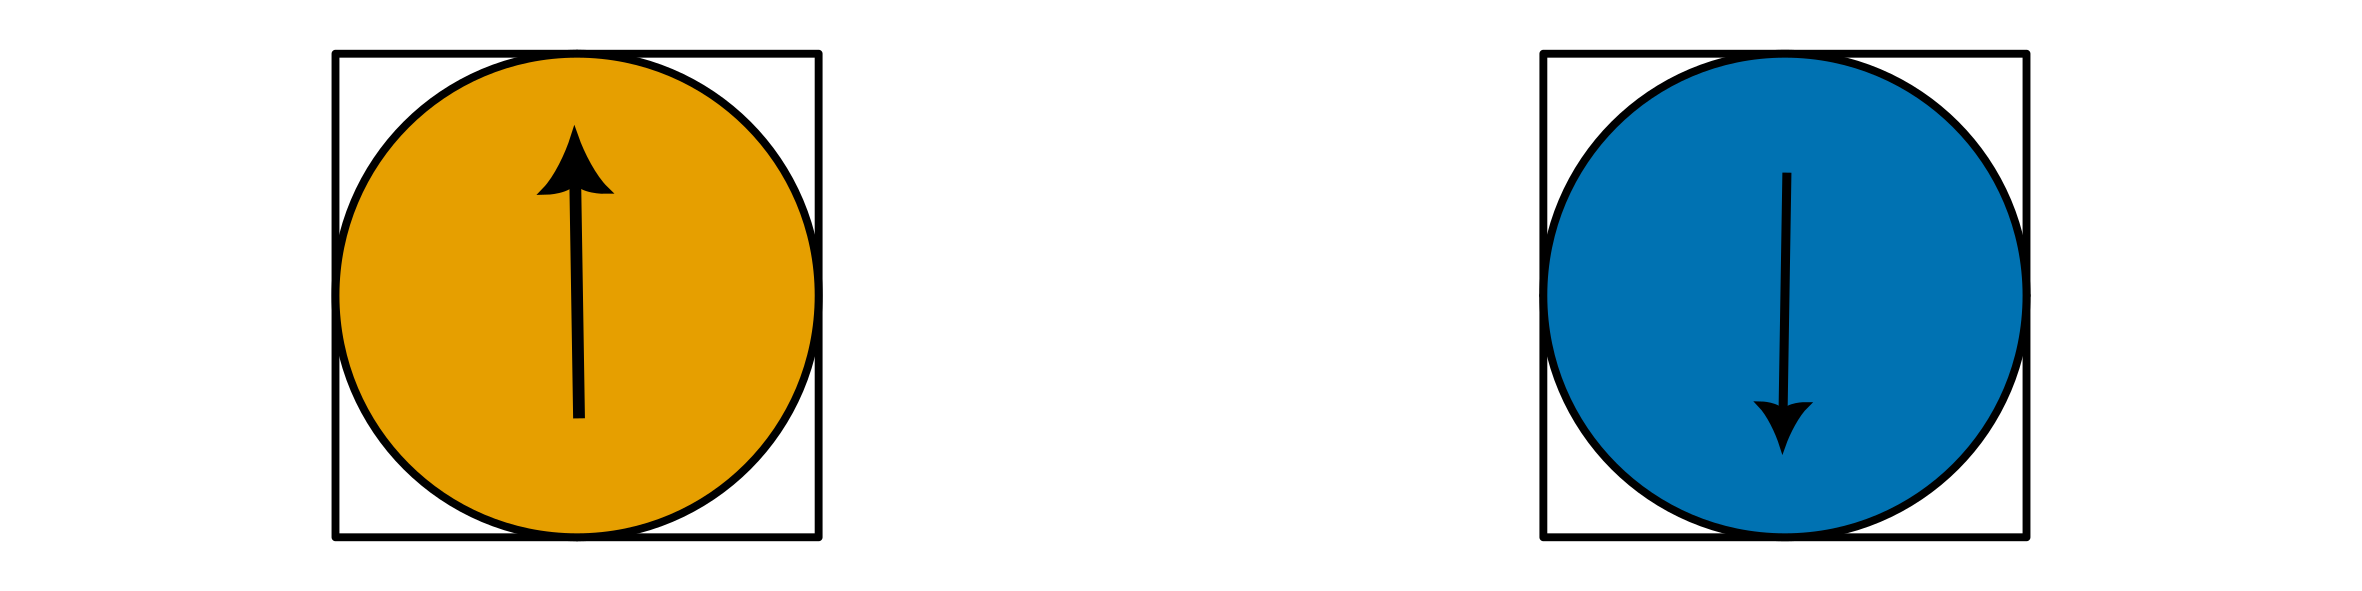
\includegraphics[width=\textwidth]{Figure 7.6.C}
\caption{Flipping a Boolean cell is a transition on a flip graph}
\end{figure}
\noindent 
The interesting thing is that states that appear similar are not necessarily adjacent on a flip graph.
\begin{figure}[H]
\centering
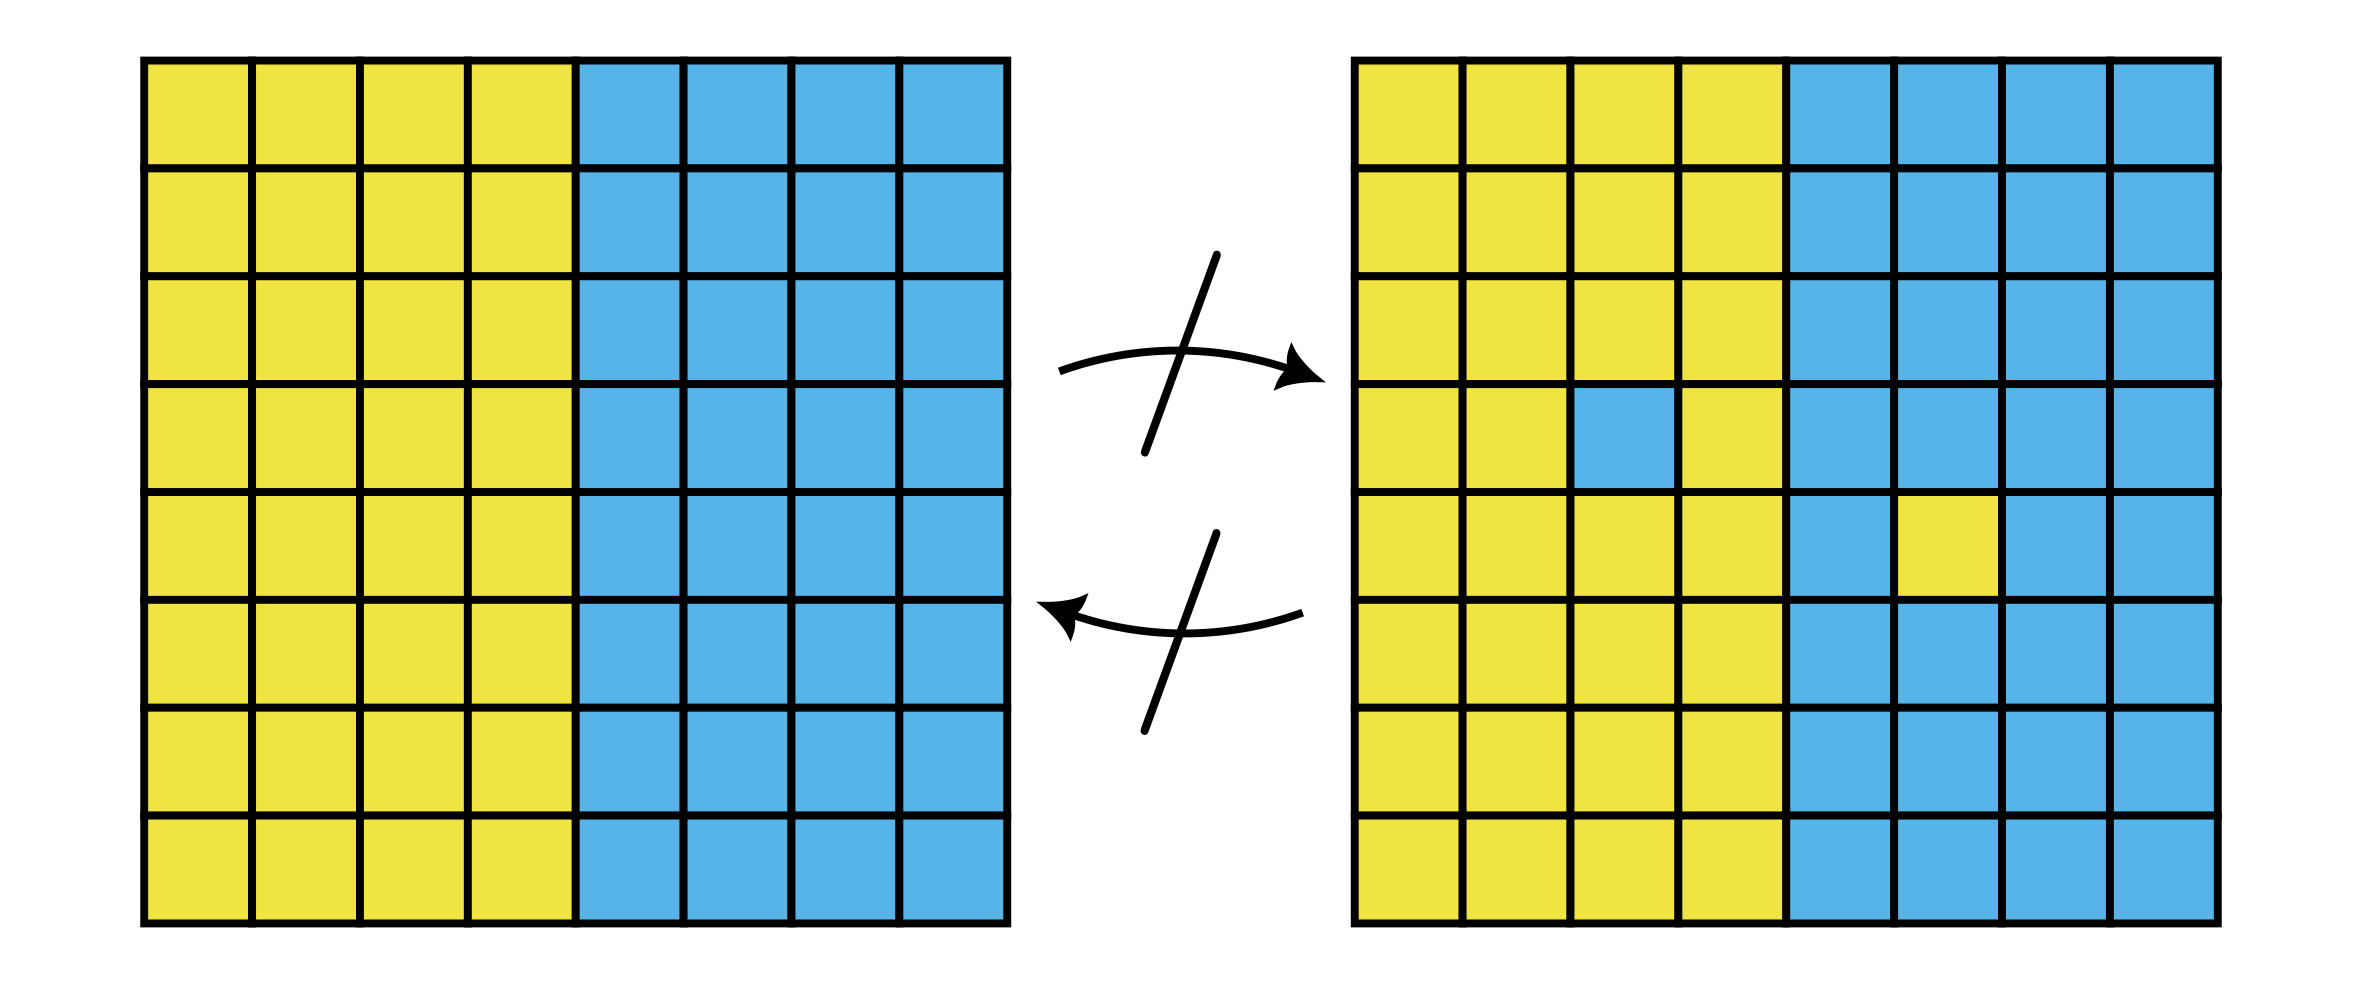
\includegraphics[width=\textwidth]{Figure 7.6.D}
\caption{Non-adjacent states of a Boolean random walk}
\end{figure}
For larger systems, such similar appearing states would function similarly along some boundary for a short period of time, but their behavior will diverge later.

\section{n-Flip Chordings and Orderings}
Every $n$-flip operation of a Boolean random walk has a number of valid chordings $c$ and exactly $o=n!$ orderings of each chording. It is a type of derangement, or a arrangement permutation in which no element remains in its starting posiiton. What is a chording? Consider the following subsystem $S_t$ of a Boolean mechanical system $X_t$ in which $x \in \mathbb B_\pm$, for all cells $x \in X_t$:
\begin{figure}[H]
\centering
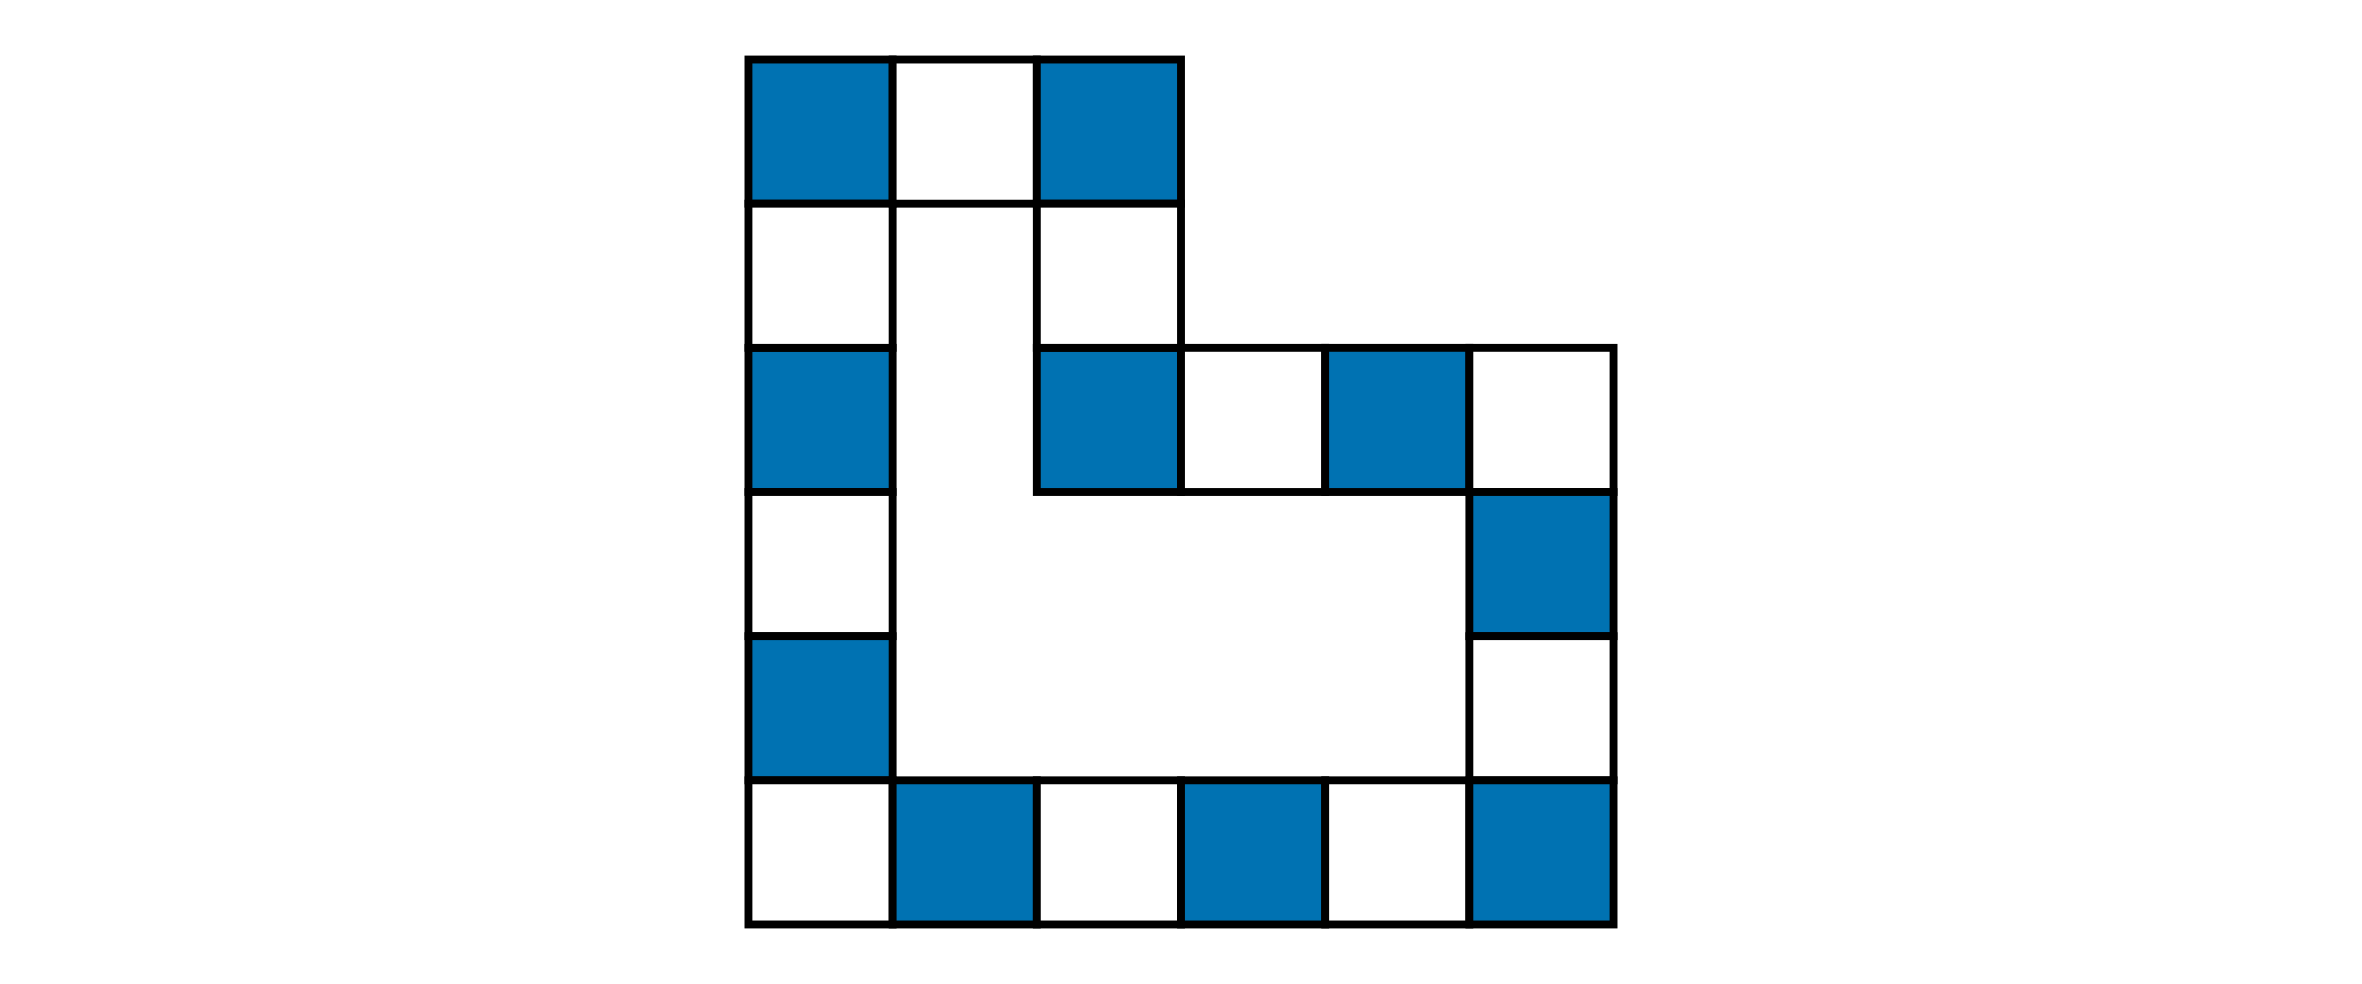
\includegraphics[width=\textwidth]{Figure 7.7.A}
\caption{A checker chain that forms a closed loop}
\end{figure}
\noindent This subsystem $S_t$ constitutes what we shall refer to as a \textbf{checker chain}\index{checker chain}. We are interested specifically in this subsystem's inversion such that $S_{t+1} = -S_t$. Upon close observation, it is possible to determine that the number of chordings for this $10$-flip operation is $c=2$:
\begin{figure}[H]
\centering
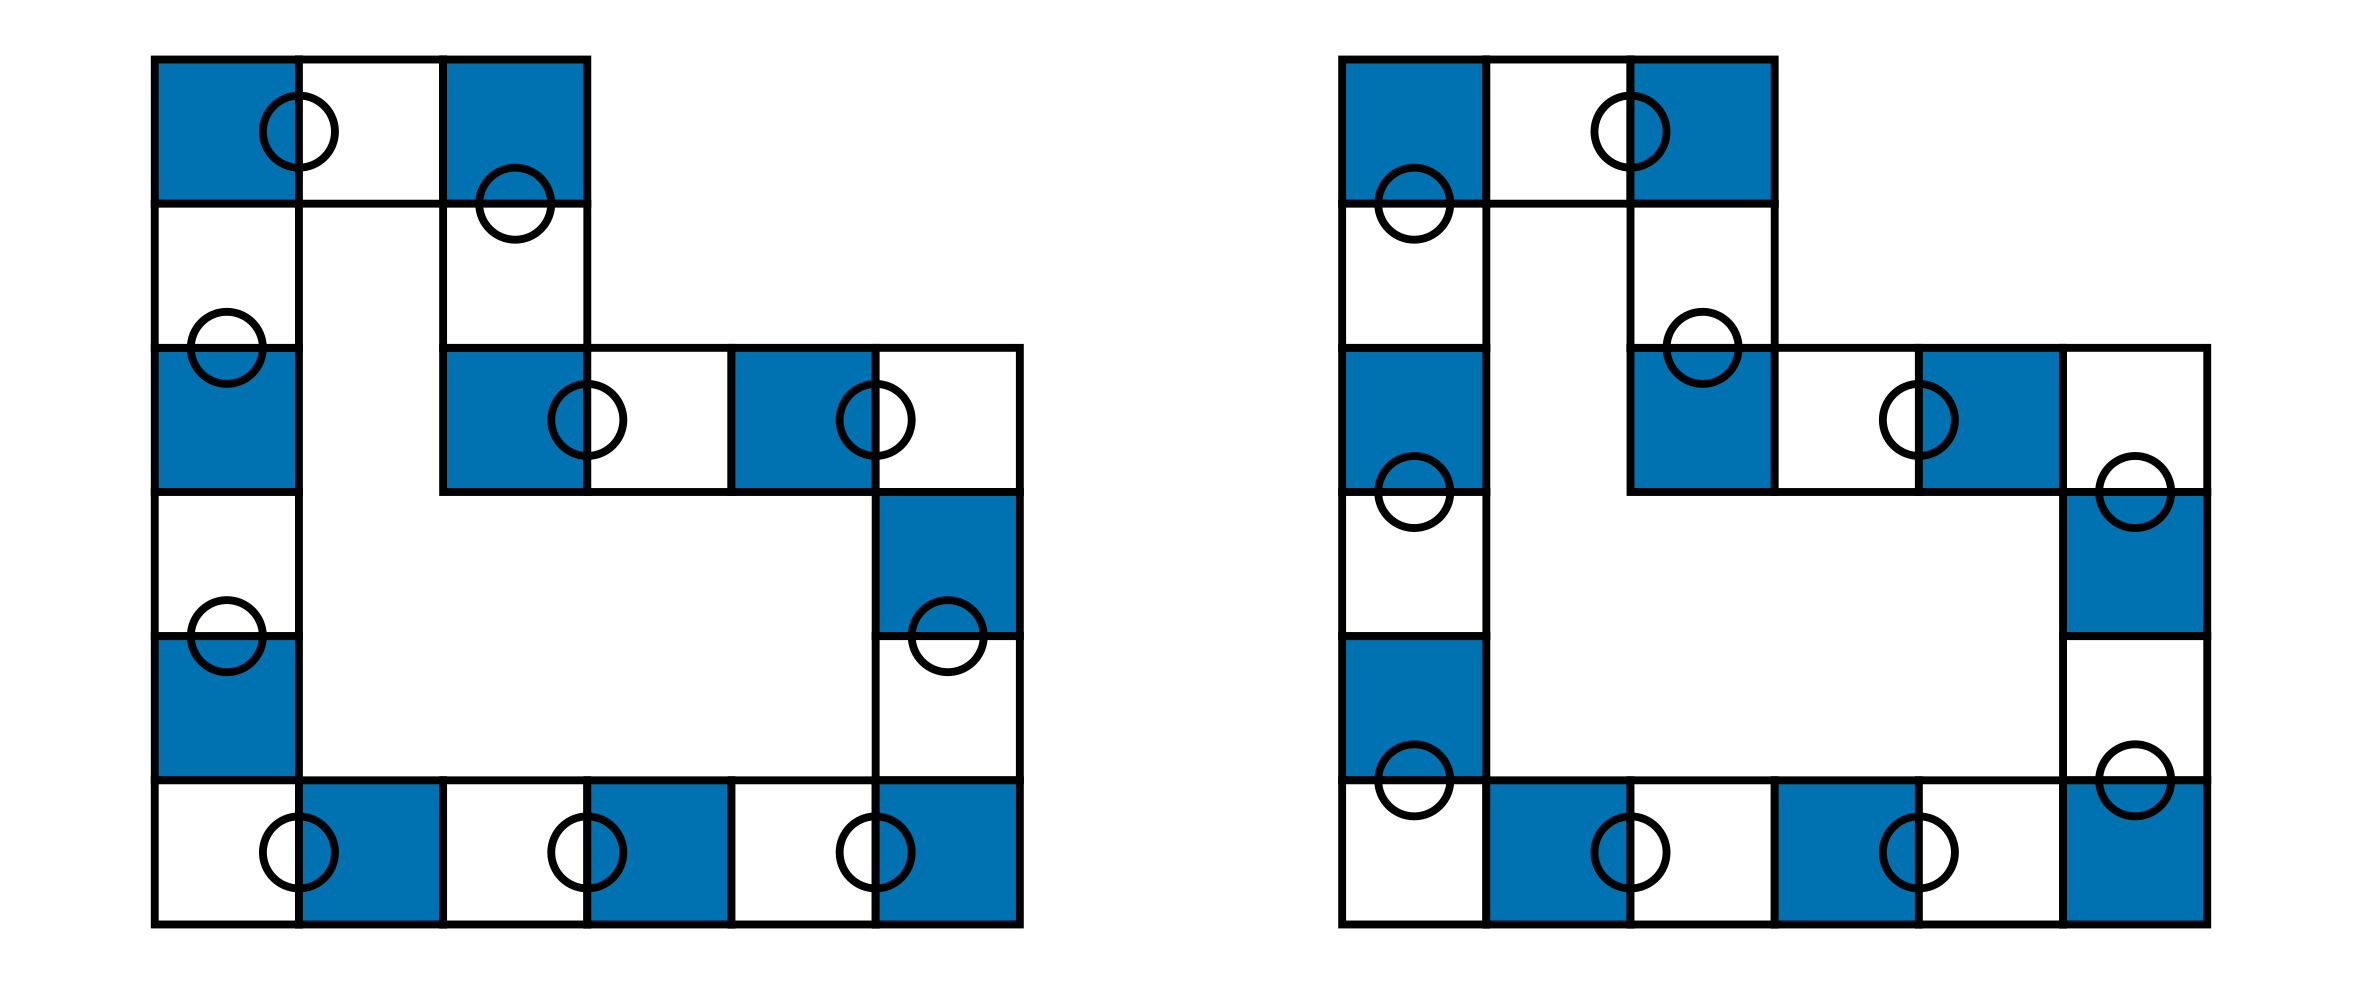
\includegraphics[width=\textwidth]{Figure 7.7.B}
\caption{This checker chain only has two possible chordings}
\end{figure}
\noindent 
There are no other possible chordings that produce the same output.

Now assume we modify $S_t$ with a checkered square added to its interior such that $S_{t+1} = -S_t$ is a $12$-flip operation:
\begin{figure}[H]
\centering
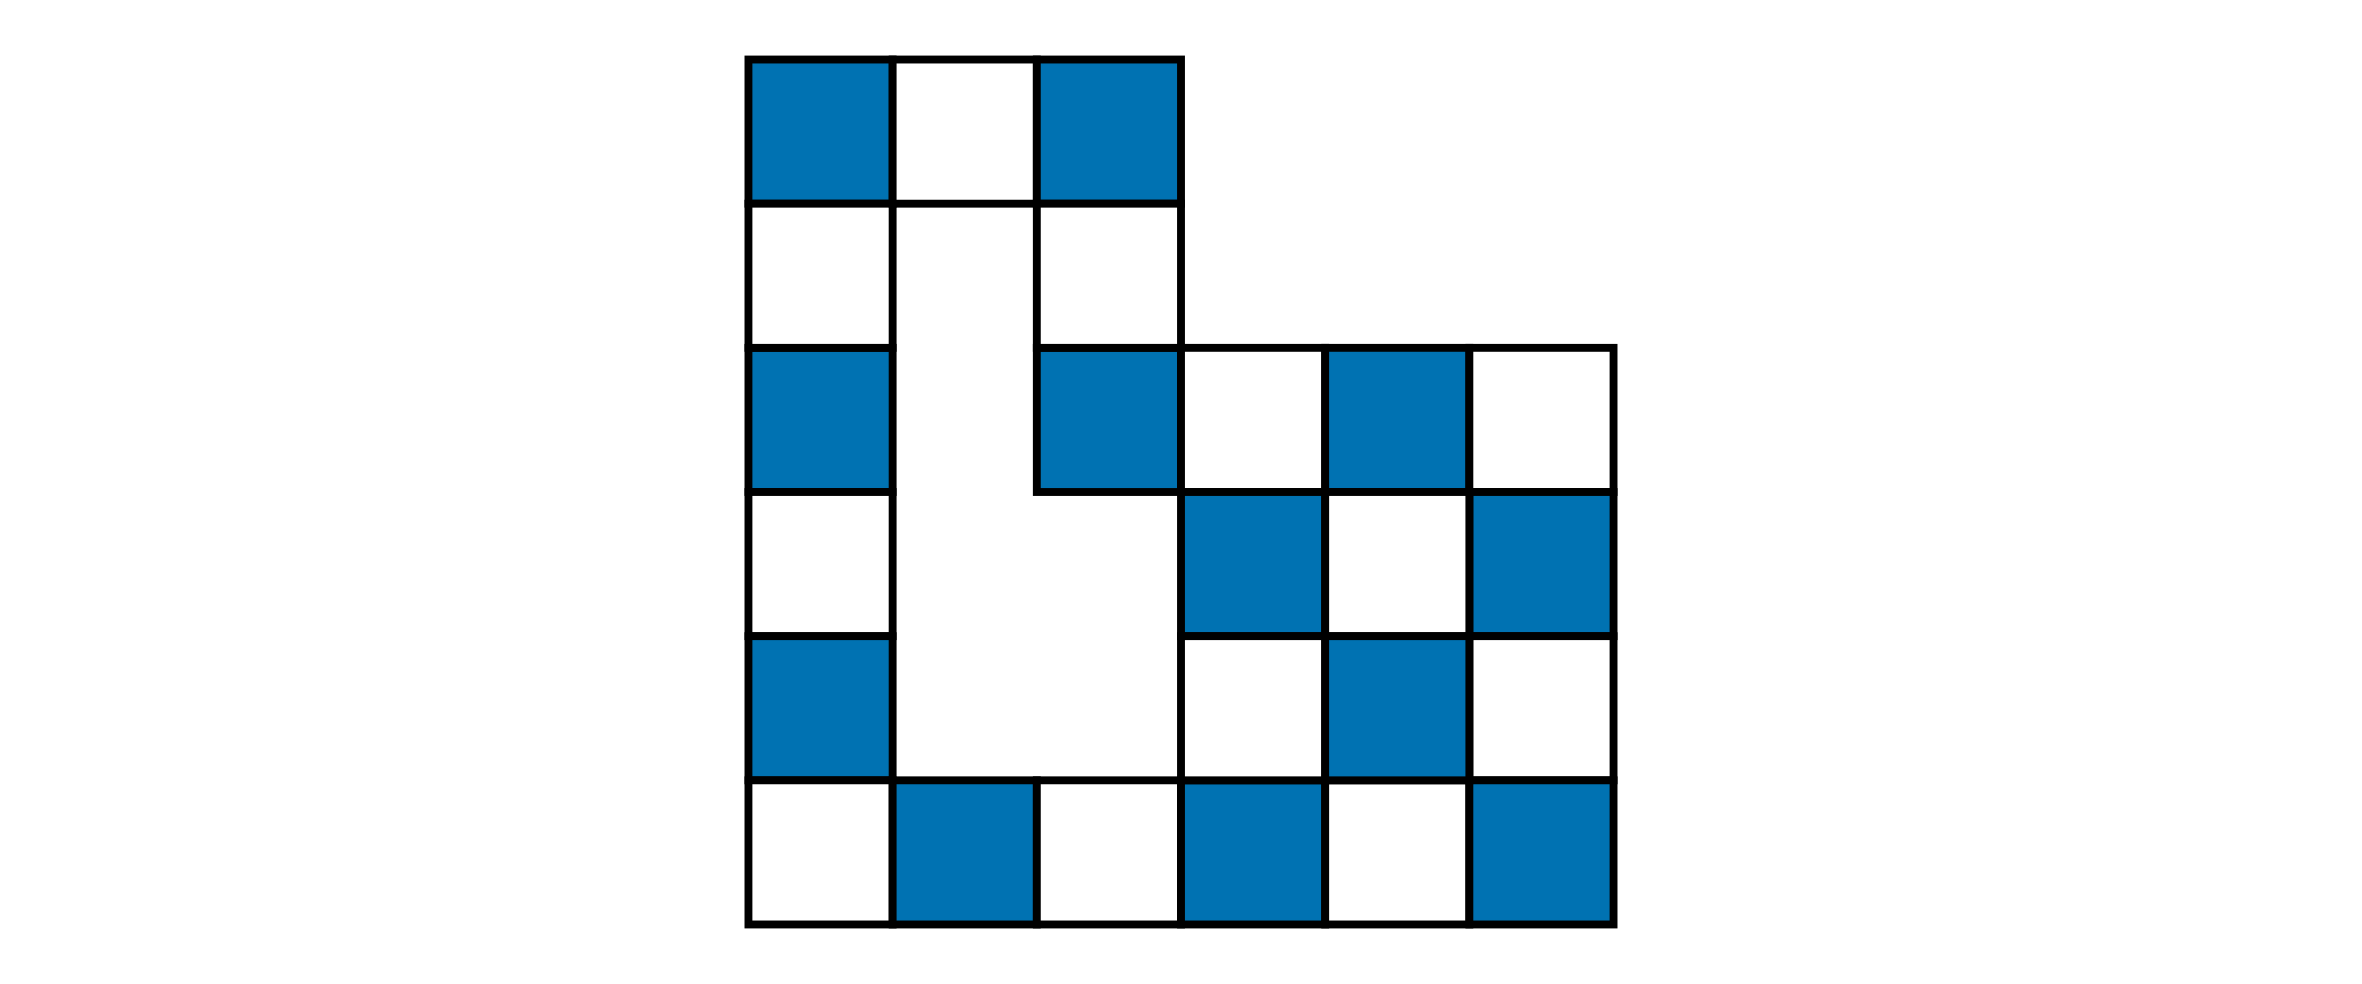
\includegraphics[width=\textwidth]{Figure 7.7.C}
\caption{An extension of the prior checker chain}
\end{figure}
\noindent 
How many valid chordings $c$ results in $S_{t+1} = -S_t$? A $2 \times 2$ checker has its standard vertical and horizontal chordings, and the original checker chain has its vertical and horizontal corners:
\begin{figure}[H]
\centering
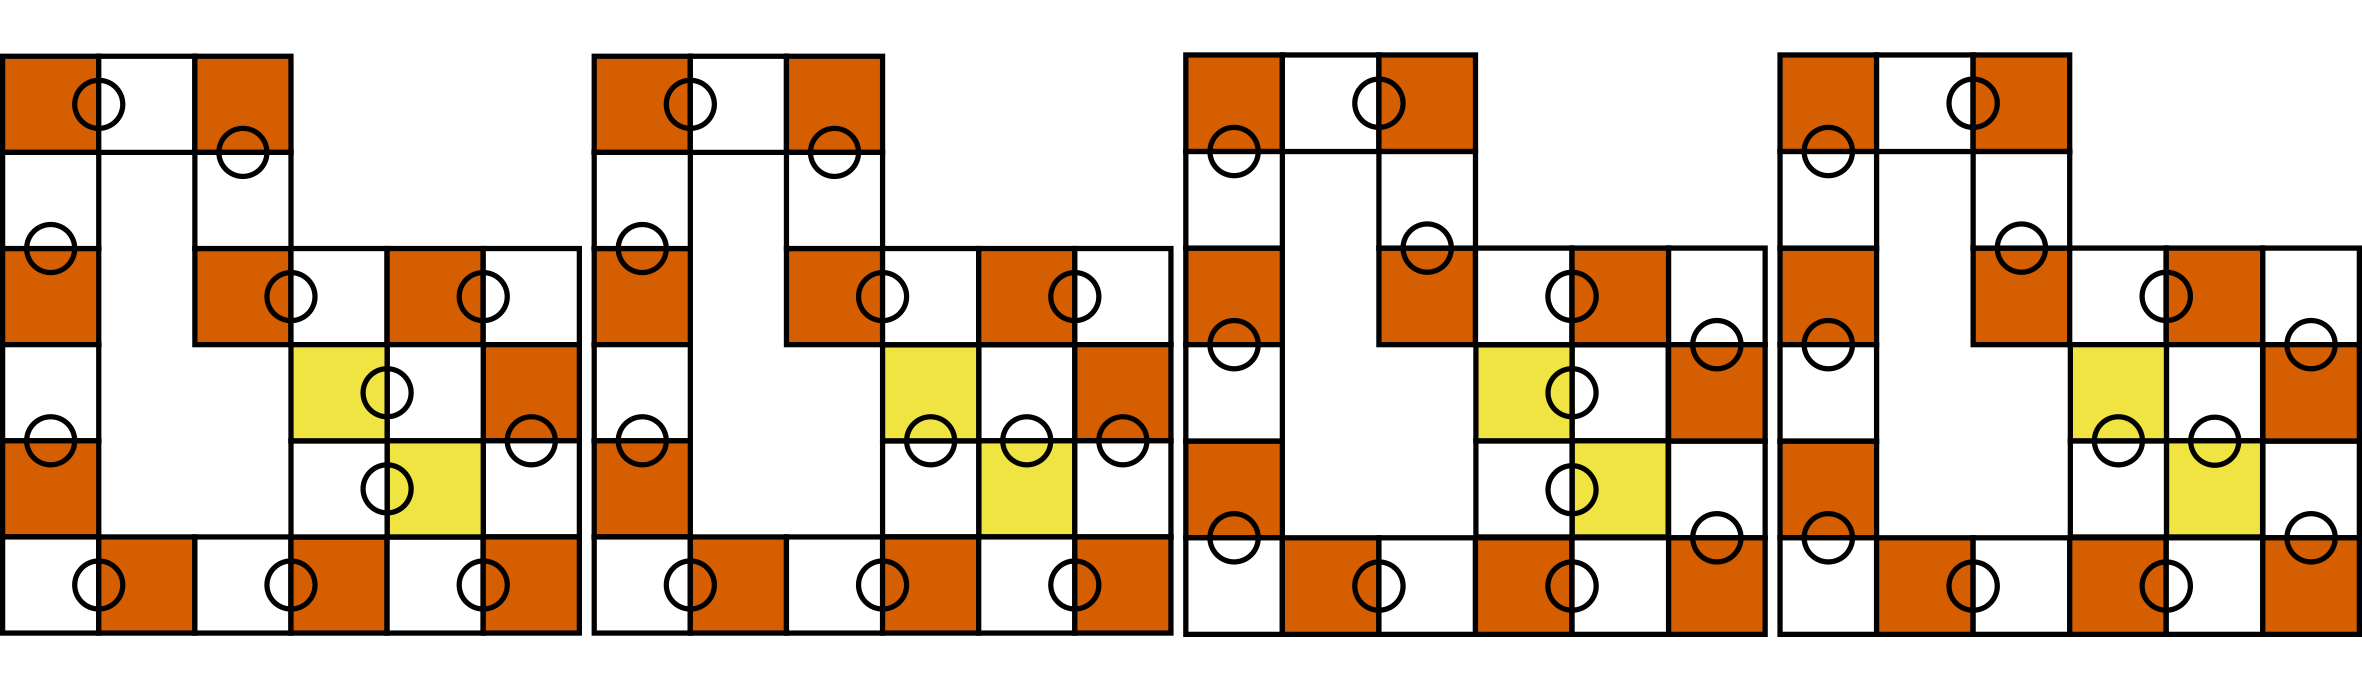
\includegraphics[width=\textwidth]{Figure 7.7.D}
\caption{Counting the elementary extension chordings}
\end{figure}
\noindent This makes a total of $4$ chordings so far, but many more non-elementary chordings were added:
\begin{figure}[H]
\centering
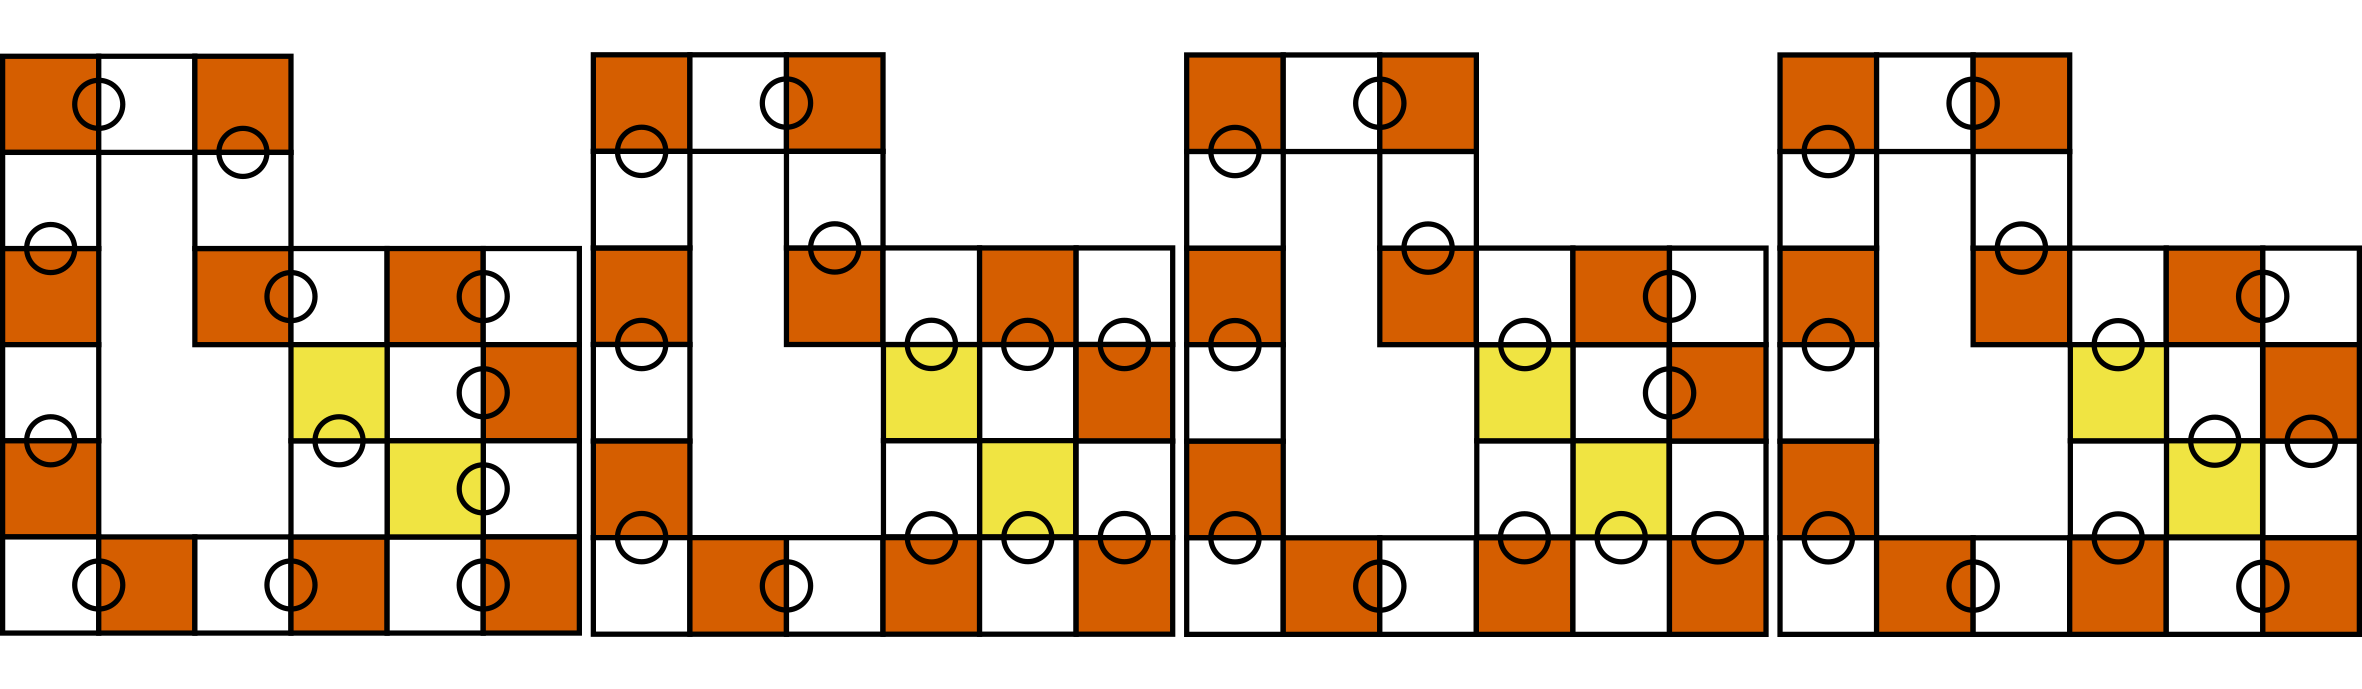
\includegraphics[width=\textwidth]{Figure 7.7.E}
\caption{Some non-elementary chordings from our extension}
\end{figure}
\noindent
There are more possible chordings than are listed here.

The identical problem that we are looking for is that of \textbf{domino tiling}\index{domino tiling} of a rectilinear region:
\begin{figure}[H]
\centering
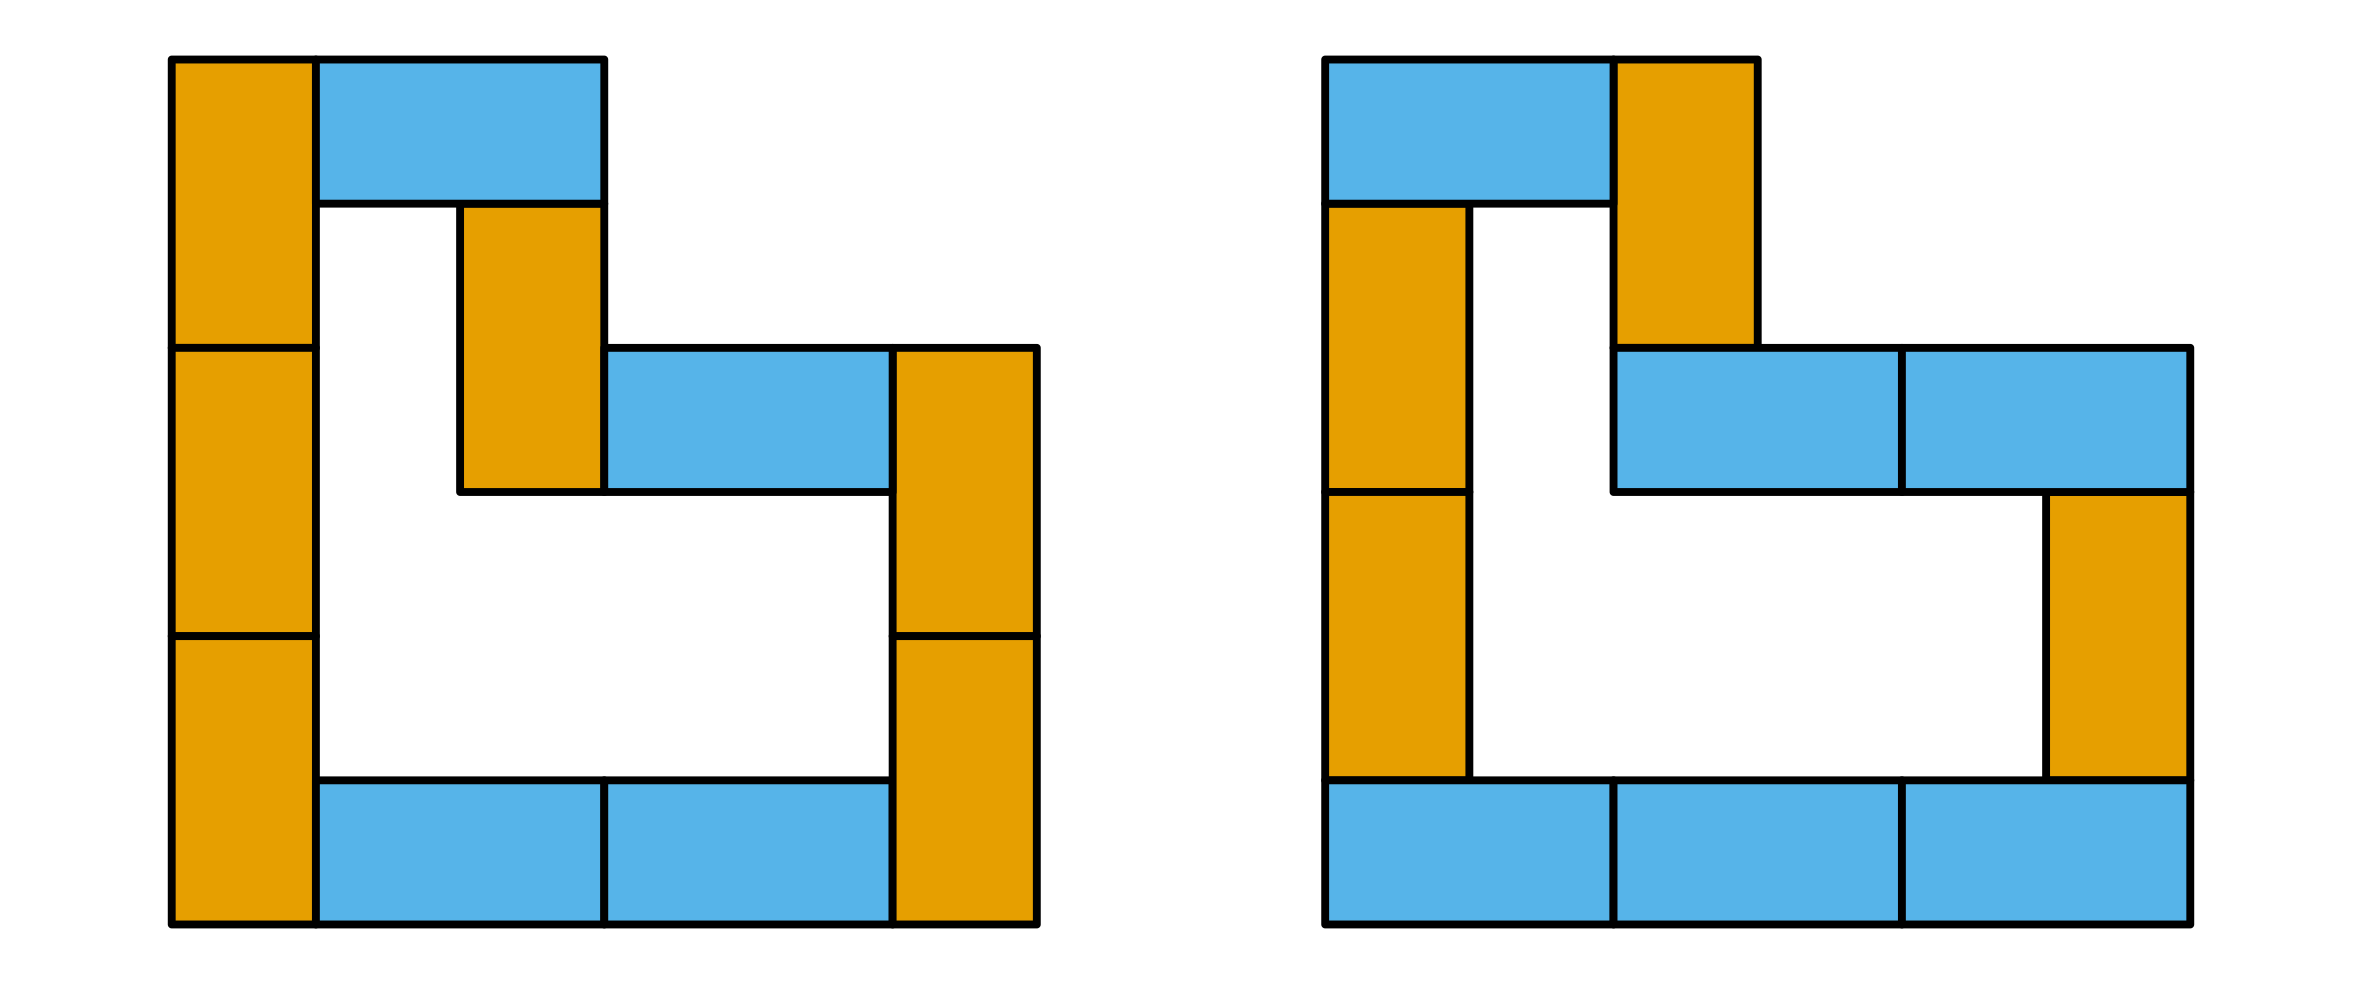
\includegraphics[width=\textwidth]{Figure 7.7.F}
\caption{The domino tiling representation of our checker chain transition}
\end{figure}
\noindent
Counting the number of valid domino tilings has a formula when they are rectangular regions in 2D without holes. However, in 3D or irregular regions has no specific formula.\footnote{The domino tiling of a $2 \times n$ room is given by the Fibonacci sequence.}

In fact, the \textbf{tatami}\index{tatami} tiling of an irregular room is \textbf{NP}-complete.
\begin{figure}[H]
\centering
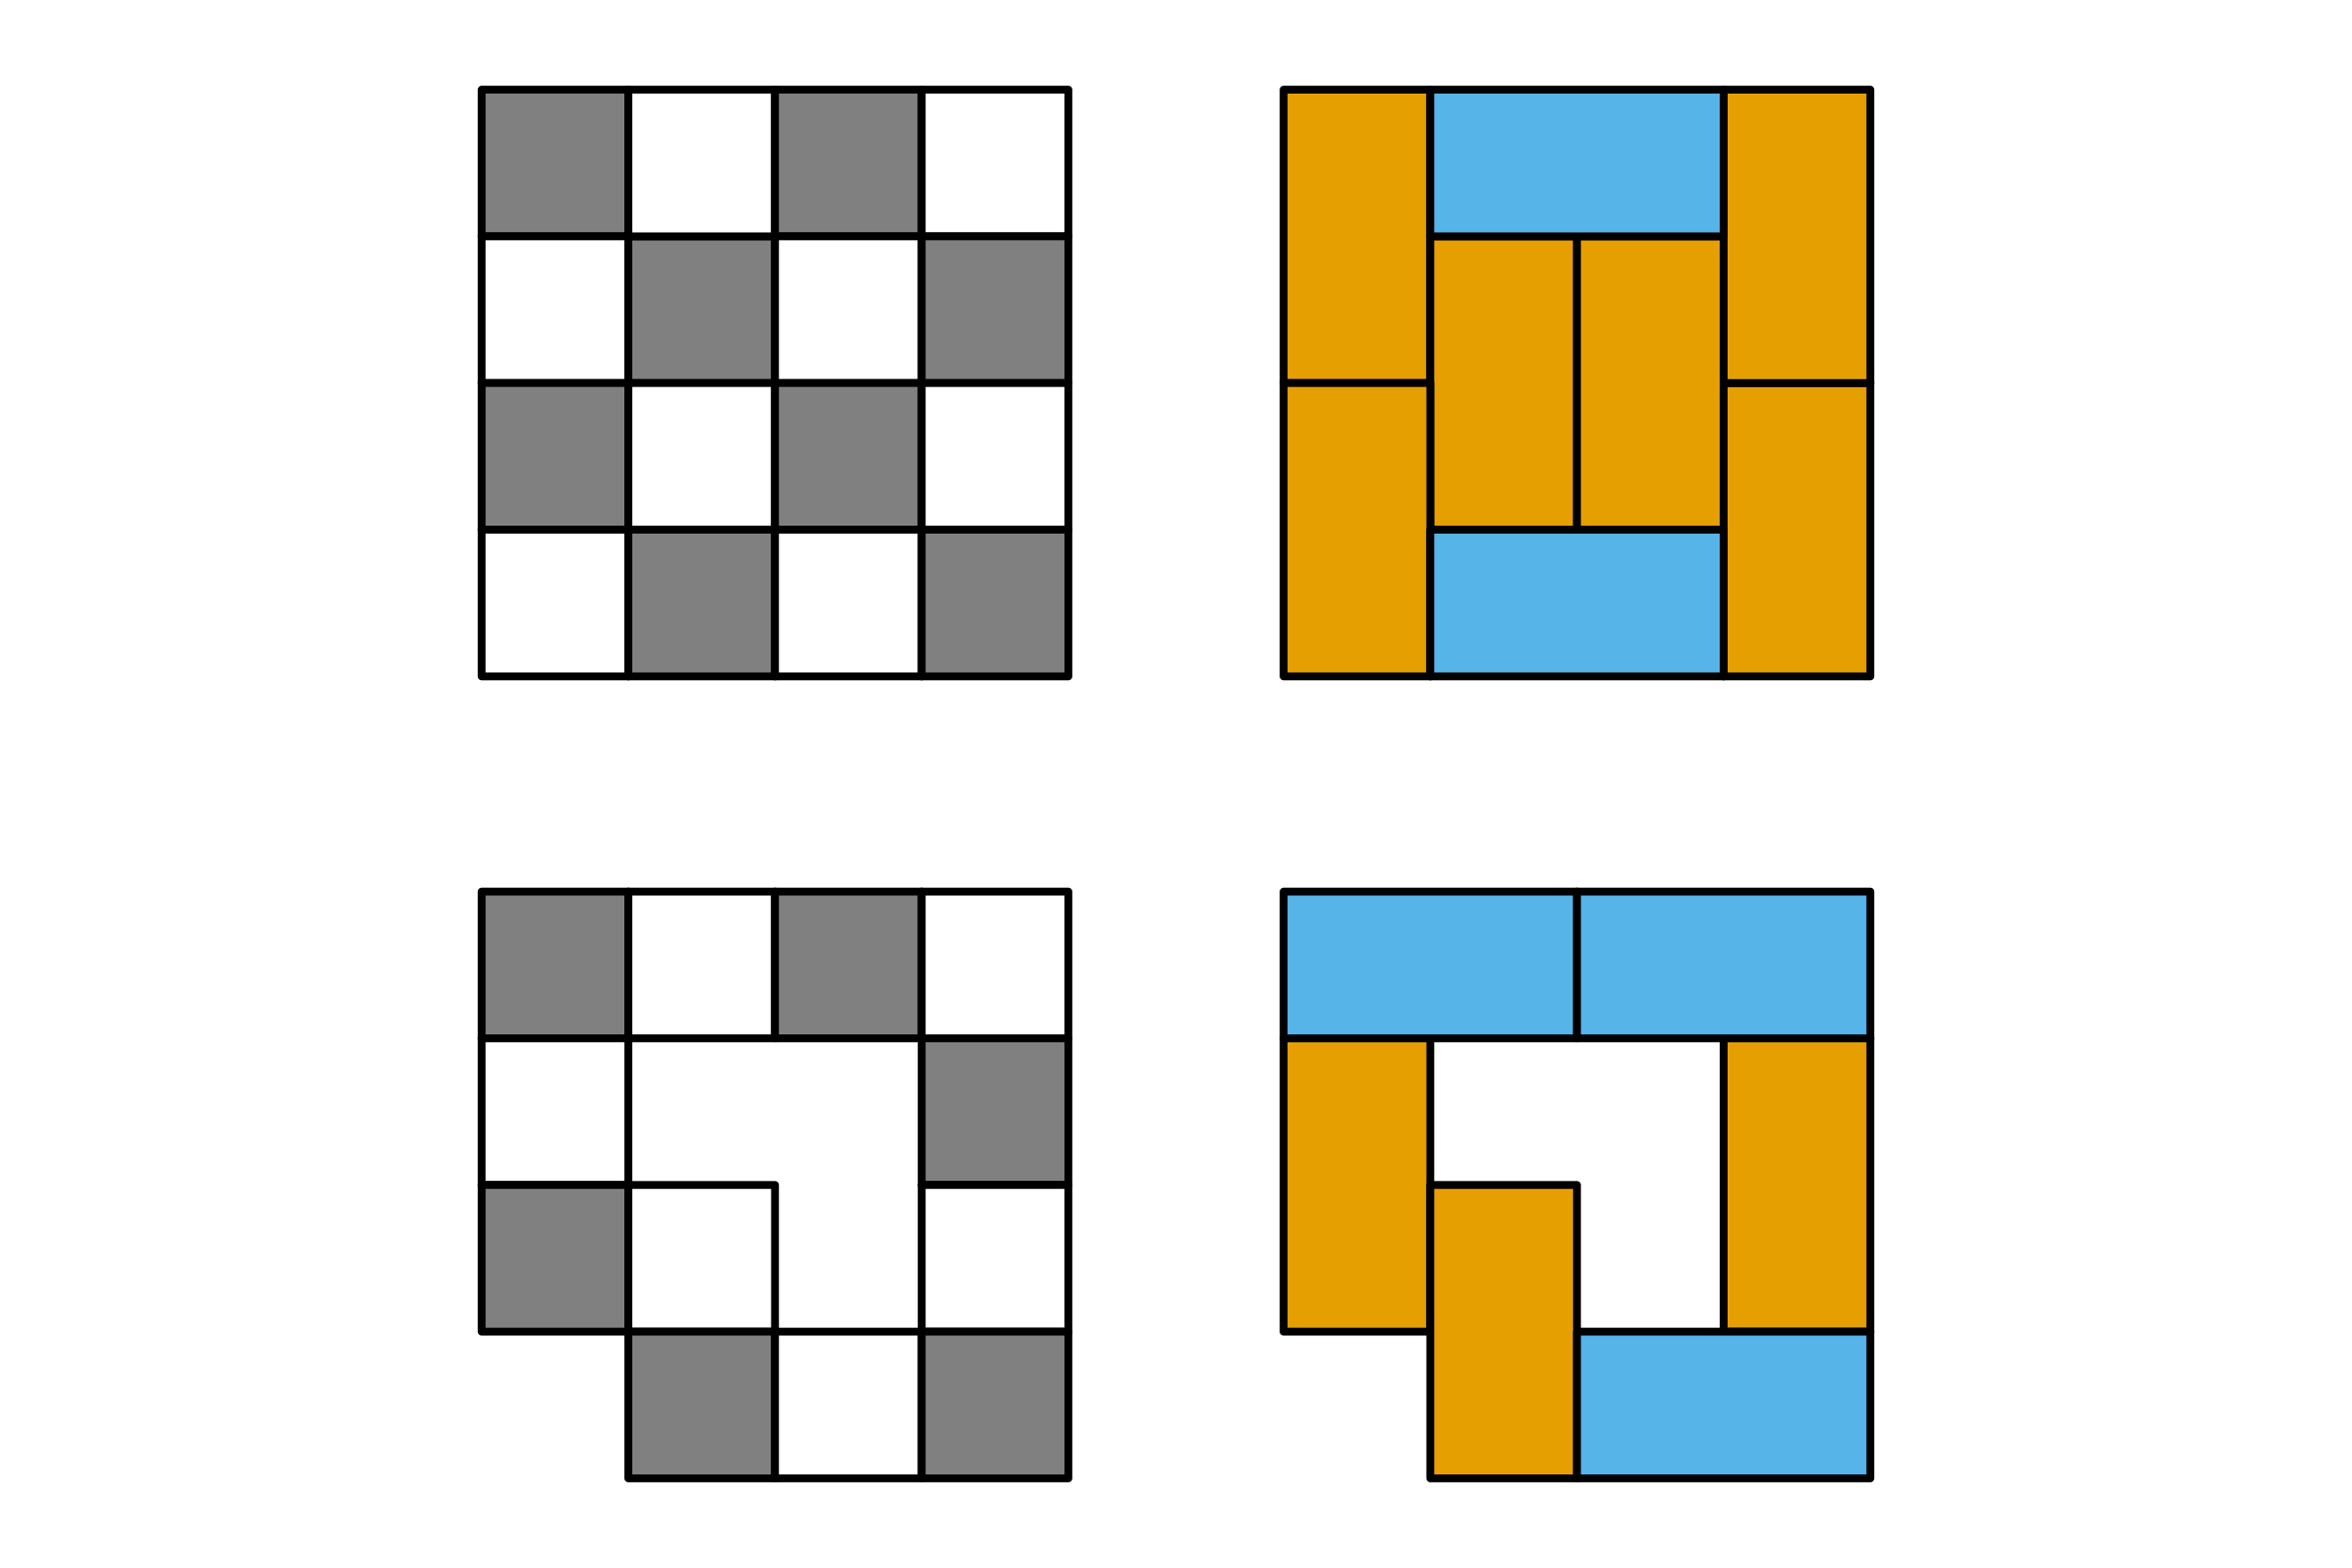
\includegraphics[width=\textwidth]{Figure 7.7.G}
\caption{Tatami tiling of a rectangular and non-regular room}
\end{figure}
\noindent
A tatami tiling has no more than three rectangles touching any corner. A regular room is any rectangular room without holes. 

The idea of ``irregular'' rooms occurs frequently in a Boolean random walk. There is therefore no efficient algorithm to calculate the number of unique chordings $c$ for a given transition $S_t \rightarrow S_{t+1}$. Suppose that $S_t$ is the subsystem of $X_t$ that always switches and the rest of $X_t$ stays the same such that:
$$S_{t+1} = -S_t$$
$$X_{t+1} / S_{t+1} = X_t / S_t$$
for all time $t \in \mathbb N$. All chordings $S_t \rightarrow S_{t+1}$ are domino tilings between particles and antiparticles, allowing us to define the problem in a special way.

A valid transition of a Boolean random walk is given by some maximal independent set of the finite-difference hypergraph. An \textbf{independent set}\index{independent set} is a subset of vertices on a graph that is not connected to any other vertex in the set. A \textbf{maximal independent set}\index{maximal independent set} is an independent set in which no vertices may be added to the set and still be independent:
\begin{figure}[H]
\centering
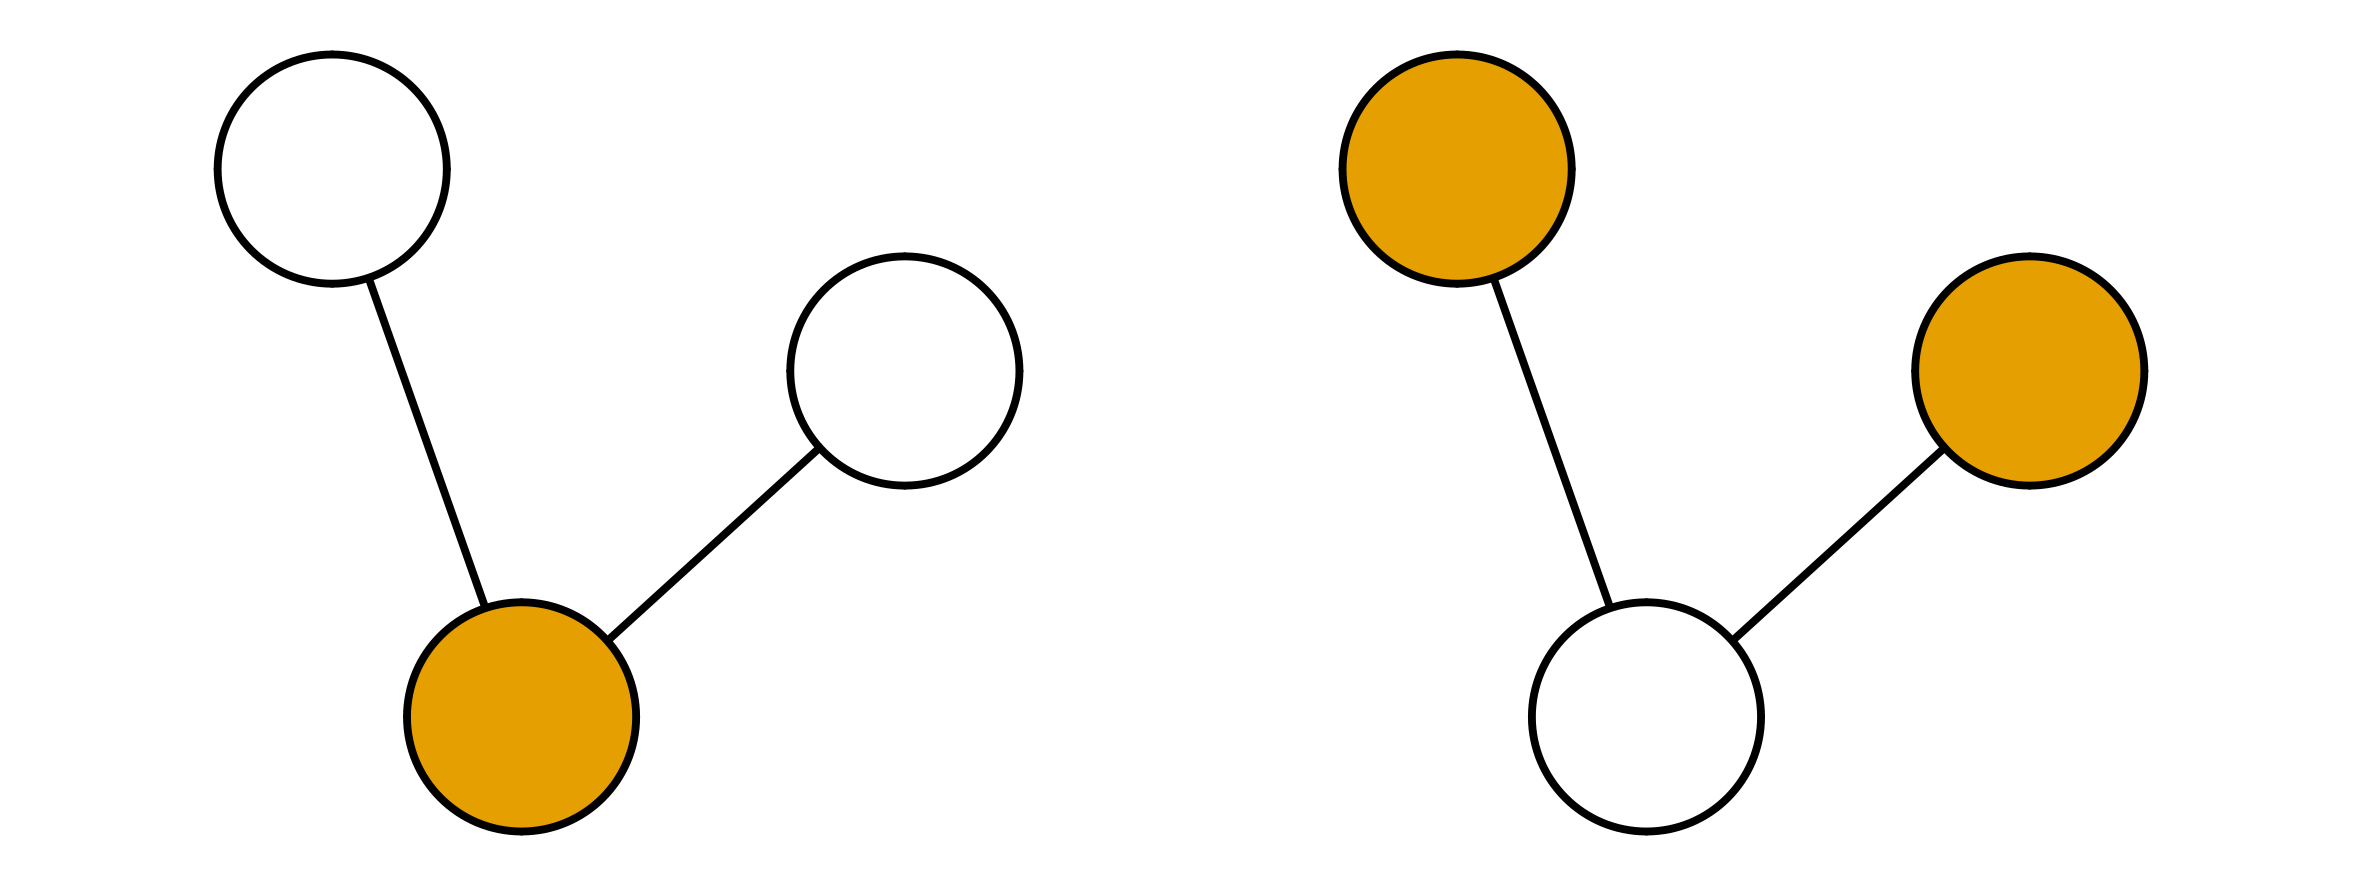
\includegraphics[width=\textwidth]{Figure 7.7.H}
\caption{All maximal independent sets of a graph}
\end{figure}
\noindent
The set of all maximal independent sets contains one or more sets with the most vertices. The computational complexity of listing all maximal independent sets of a graph is \textbf{\#P}, the enumeration of sets that some fulfill \textbf{NP} decision problems. 

It is worth noting that a maximal independent set is equally a minimal dominating set. A \textbf{dominating set}\index{dominating set} is a set in which a vertex is either in $H$ or a neighbor of $H$. A \textbf{minimal dominating set}\index{minimal dominating set} is a dominating set in which no vertex from $H$ may be removed and still be a dominating set.

Since we may have disconnected regions, we can parallelize computation to work on component subgraphs. A \textbf{component subgraph}\index{component subgraph} is a subset of a graph that is connected and not a subset of any other graph.
\begin{figure}[H]
\centering
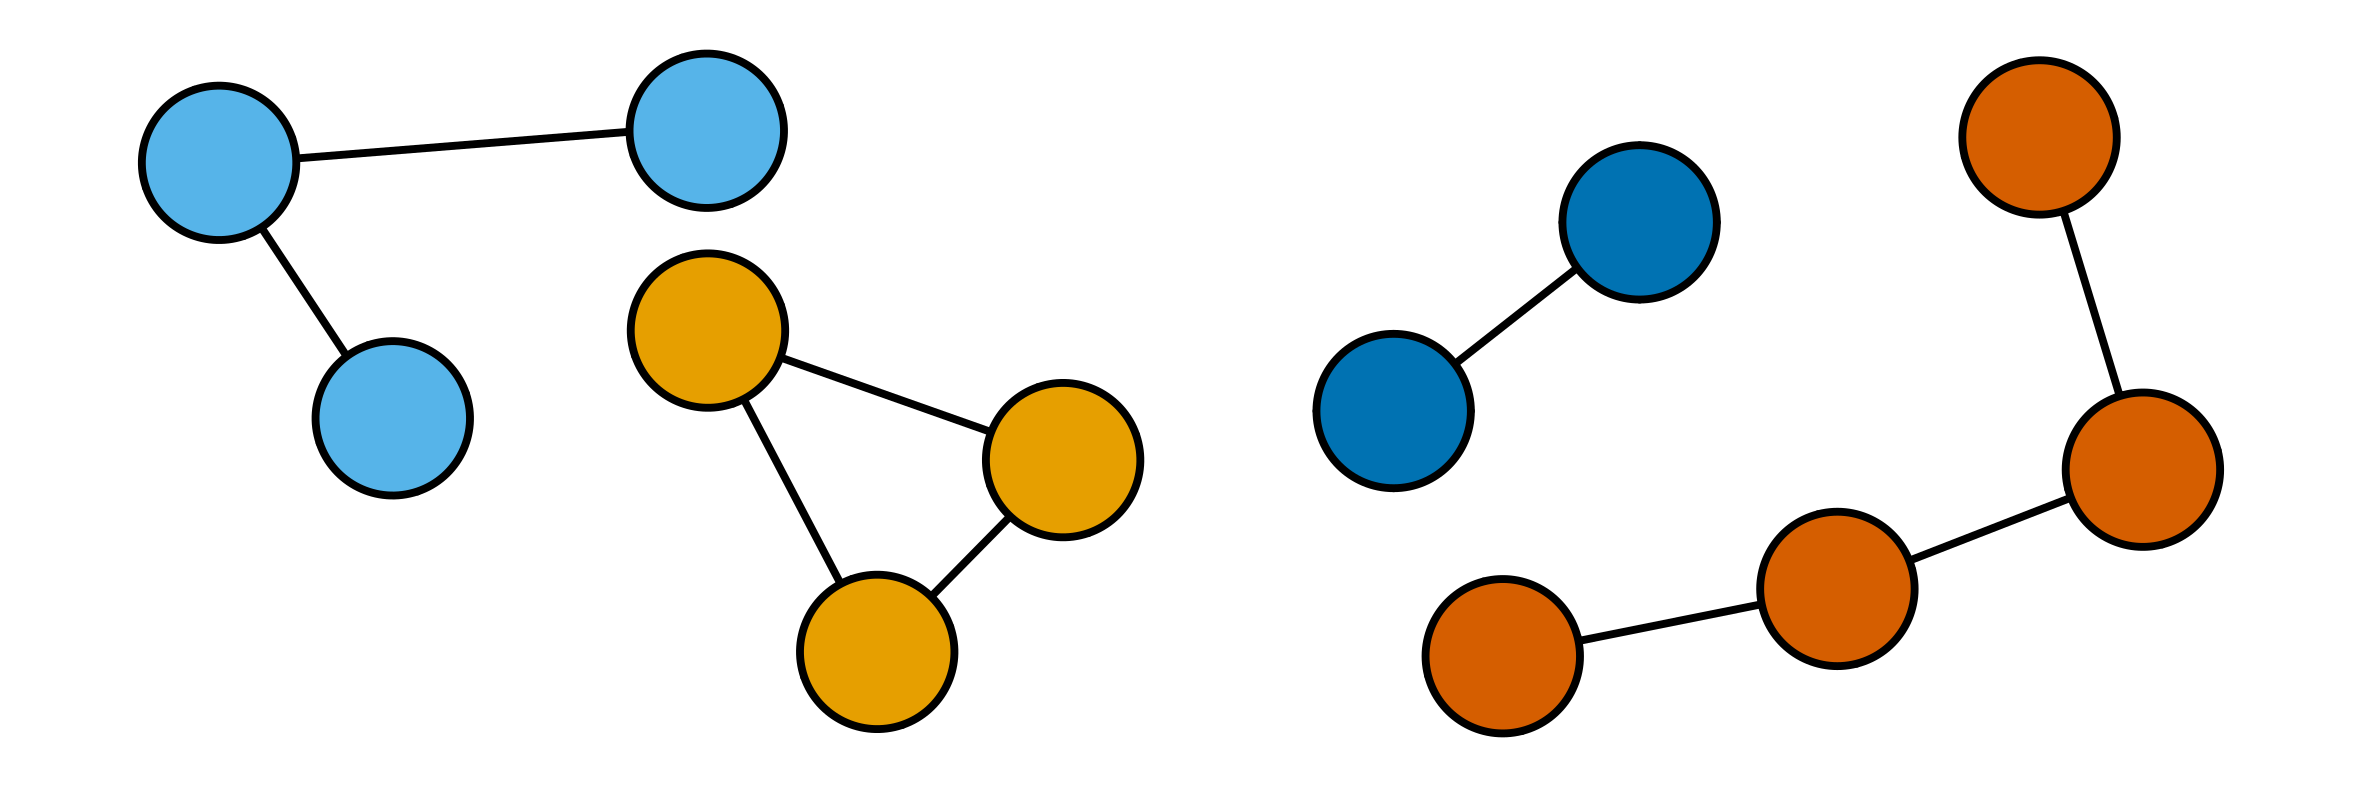
\includegraphics[width=\textwidth]{Figure 7.7.I}
\caption{A graph with $4$ components}
\end{figure}
\noindent
A relatively large Boolean random walk often has several components. As a maximal independent set of vertices become chosen, the graph becomes more disconnected. This provides an opportunity to speed up computation by some sort of divide and conquer strategy. For an algorithmic speedup unique to Boolean random walks, see \textit{\S Appendix E: Random Backtrack Algorithm}.

In order to calculate a maximal independent set, we must generate a subset of vertices from $|\Delta X|$. Let $T$ refer to the non-zero values of $|\Delta X|$. The set of vertices $H = \{{h_1,...,h_n}\}$ is initially empty. Let $\gamma$ be the neighbor function such that $\gamma(h)$ returns the set of vertices adjacent to $h$. If $H$ is a set of vertices, then $\gamma(H)$ is the union of each vertex's neighbors. We expand $H$ by adding a random element of $T$ that is not in $H \cap \gamma (H)$, and we iterate our expansions until we hit a maximal independent set. The first expansion in which we obtain our original set $T = H \cup \gamma(H)$ is the moment that $H$ is a maximal independent set and $\gamma(H)$ is a minimal vertex cover.

If this set $\gamma(H)$ is a vertex cover all vertices in a component of $T$, then we have eliminated all remaining walks in the random walk:
\begin{figure}[H]
\centering
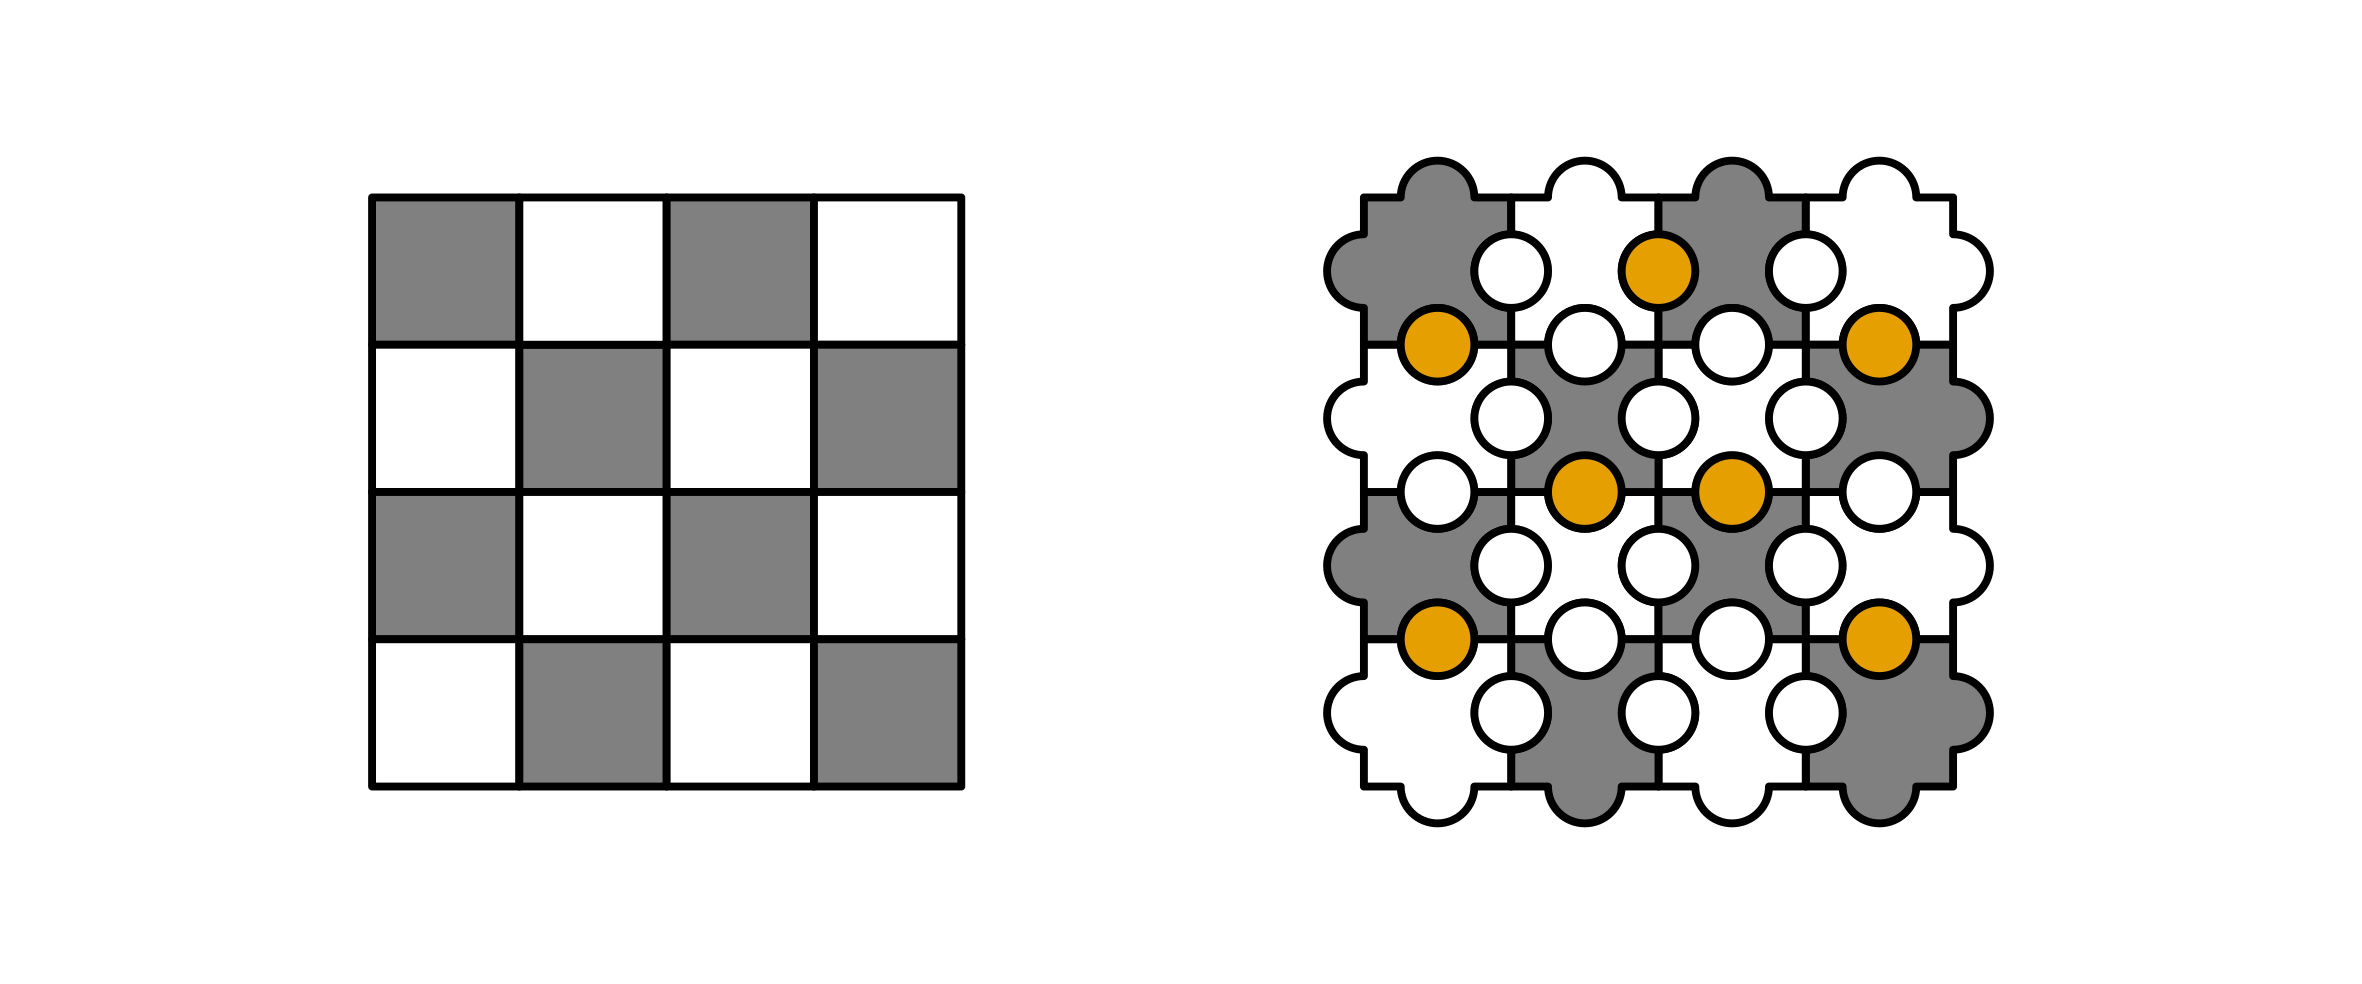
\includegraphics[width=\textwidth]{Figure 7.7.J}
\caption{Each hyperedge touches a vertex in $\gamma(H)$. Hyperedges represent Boolean cells.}
\end{figure}
\noindent
This is known as a \textbf{minimal vertex cover}\index{minimal vertex cover}. A \textbf{vertex cover}\index{vertex cover} uses vertices that connect to every edge of a component, and a minimal vertex cover cannot remove a vertex without failing to be a vertex cover. A maximal independent set of vertices (MIS) is the complement set of a minimal vertex cover (MVC) because adding more vertices to the MIS set fails the independent set criterion and removing vertices from the MVC set fails the vertex cover criterion.

Knowing that a Boolean random walk transition is the exactly problem of finding \textit{a single} maximal independent set (MIS) or minimal vertex cover (MVC), we know that the problem is of \textbf{NP} complexity. This means listing \textit{all} MIS for a specific Boolean random walk configuration state $\hat X$ is of \textbf{\#P} complexity, the complexity class of the enumeration of solutions of some \textbf{NP} problem. Calculating the stochastic matrix $P$ is likewise of \textbf{\#P} computational complexity since we do it for every initial state.

We may formalize the problem statement in the following way. Assume that each configuration of $X_t$ is from the ordered set of configurations $\mathcal X = (\hat X_1,..., \hat X_\theta)$. Each element $x$ in the configuration $\hat X$ is Boolean $\mathbb B_\circ = \{-1, +1\}$. Let $|\Delta X_t|$ be the absolute value of finite differences of $X_t$, and let $V$ be vertices referring to the non-zero values of $|\Delta X_t|$. A maximal independent set $H$ to represent a Boolean random walk transition $f: X_t \rightarrow X_{t+1}$ has the following properties:
\begin{quote}
$H \subseteq T$: $H$ is a subset of all vertices $T$

$H \cap \gamma(H) = \varnothing$: $H$ is an independent set

$H \cup \gamma(H) = T$: $\gamma(H)$ is a vertex cover, equivalently $H$ is a dominating set

$X_{t+1} = (-\Delta^{-1} H) \cdot X_t$: The transition map $f: X_t \rightarrow X_{t+1}$ selects then inverts hyperedges $h$ in $H$.
\end{quote}
Note that $H$ is an independent set \textbf{AND} a $\gamma(H)$ is a vertex cover if and only if $H$ is a maximal independent set \textbf{OR} $\gamma(H)$ is a minimal vertex cover. 

Generating an MIS/MVC from a graph $G$ is simple. Initialize $H$ as empty and assign $\Delta X_t$ to $G$. Randomly sample a vertex from $G$ to add to $H$. Remove that vertex and adjacent vertices from $G$. Repeat until $G$ is empty. We can enumerate all possible transitions using a deterministic algorithm that considers all sampling orders upon vertices in $G$. If we are trying to construct stochastic matrix $P$ this way, it will oversample the chordings of any transition proportionally.
\begin{figure}[H]
\centering
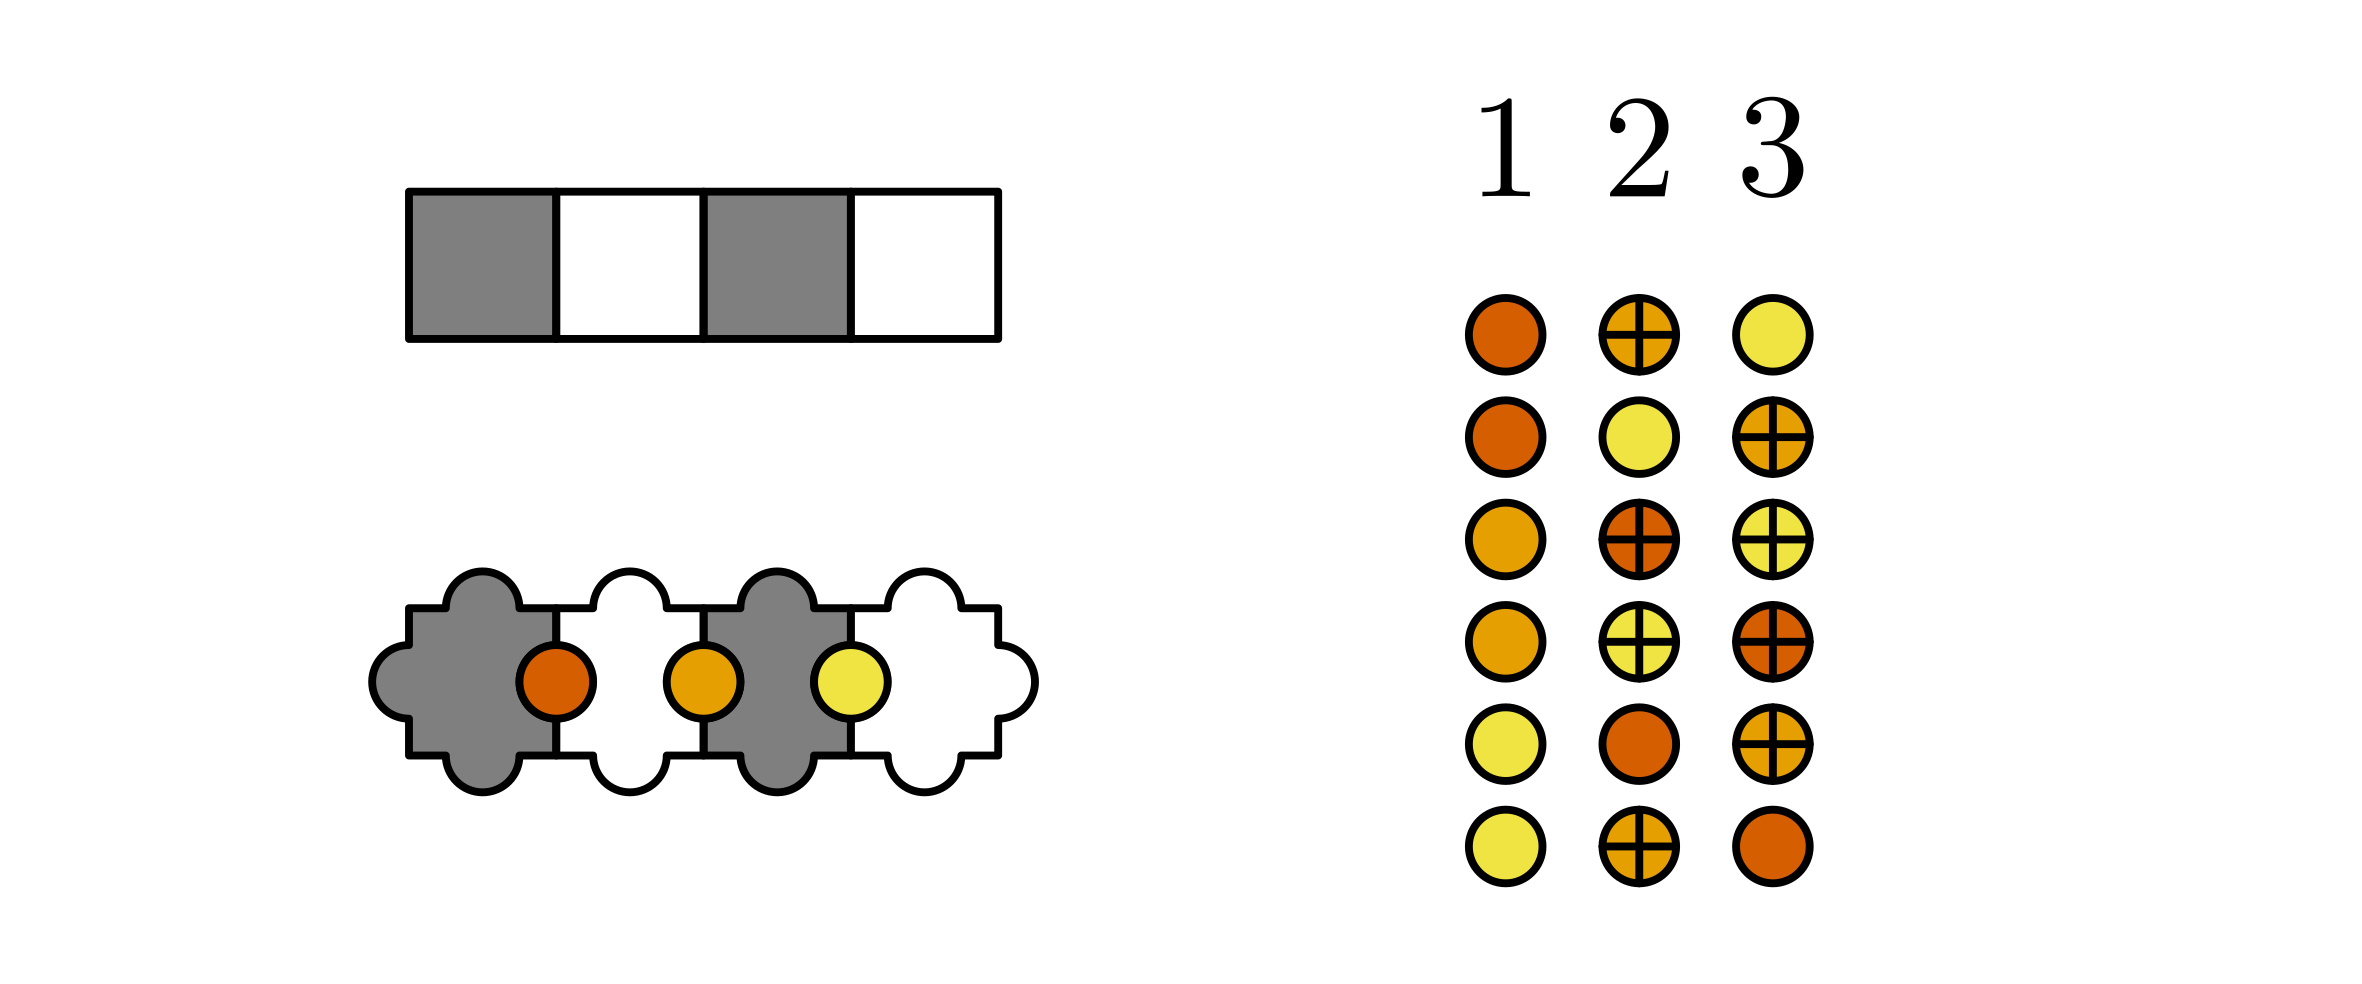
\includegraphics[width=\textwidth]{Figure 7.7.K}
\caption{Eliminated vertices are oversampled proportionally}
\end{figure}
\noindent
The oversampling of maximal independent sets is given by $2^{|\Delta X| - |H_{\max}|}$. $|H_{\max}|$ is the number of vertices in \textit{the maximum independent set} of the maximal independent sets.

This minimalist formalist description may not feel quite as physically intuitive as we might like. A more physics-oriented motivation is given in \textit{\S 11.3 Boolean Hamiltonians}. In Boolean random walks, a set $H$ which fits this description is a valid Hamiltonian or total energy. We call the set $T$ from the non-zero values of $|\Delta X|$ the kinetic energy. We call the set difference $V = T / H$ the potential energy.
\begin{figure}[H]
\centering
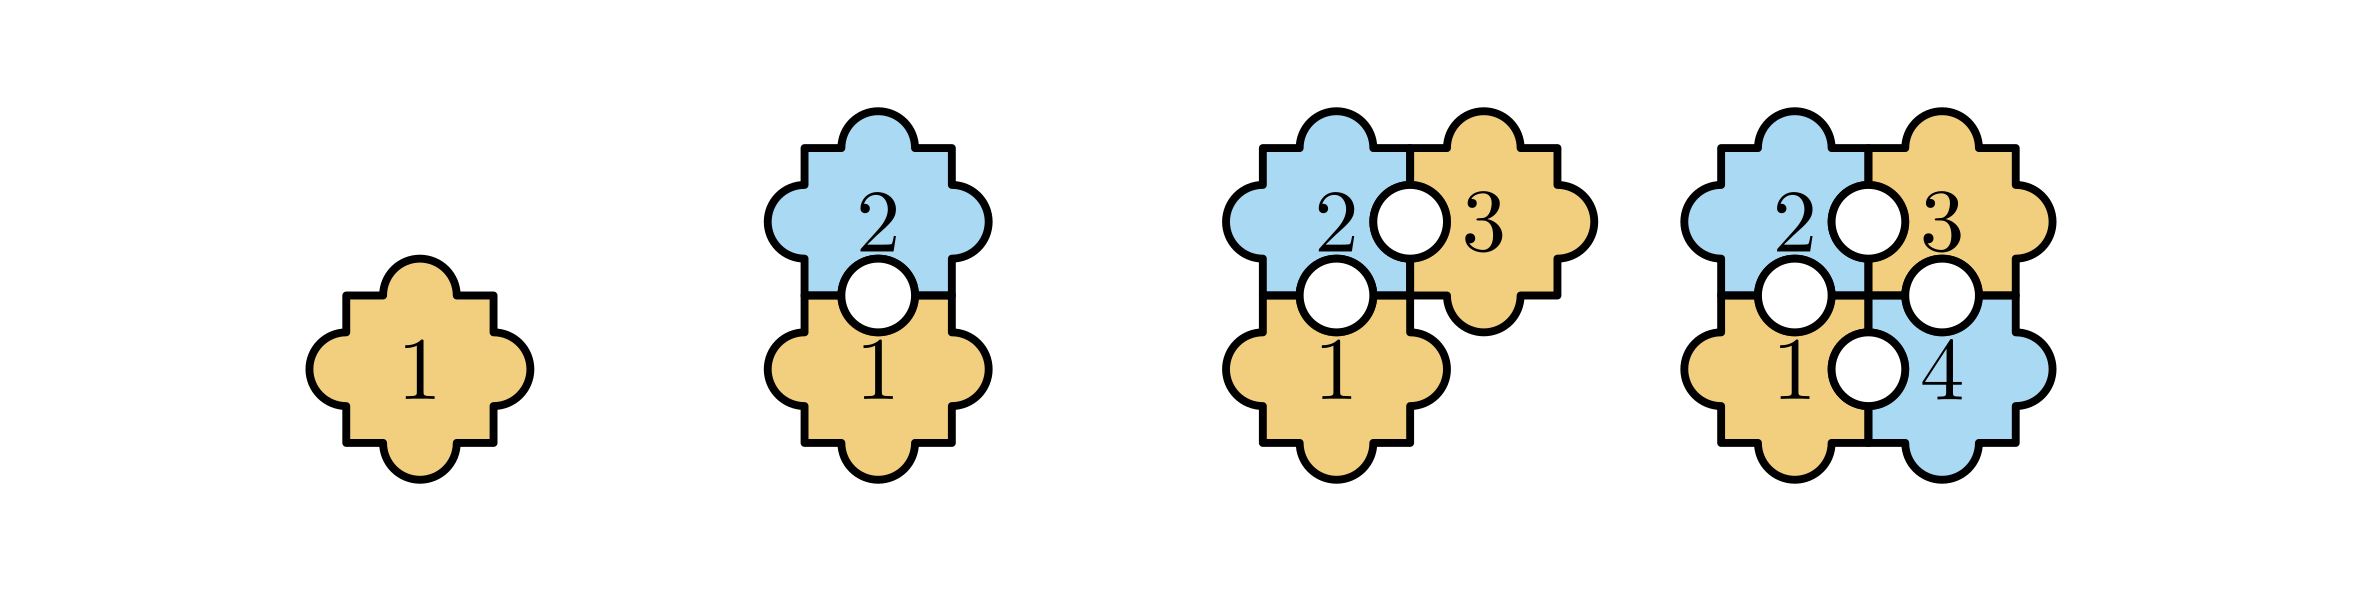
\includegraphics[width=\textwidth]{Figure 7.7.L}
\caption{The size of any maximal independent set $H$ is at most half of $T$ in 1D}
\end{figure}
\noindent Observing these graphs, we may observe it definitely true that:
$$\textnormal{vert}(H) \leq \frac{\textnormal{vert}(T)}{2}$$
$$\textnormal{vert}(V) \geq \frac{\textnormal{vert}(T)}{2}$$
This is because we can never add more vertices to $T$ than hyperedges, and remember that each hyperedge is a Boolean cell. The number of sampled vertices for our maximal independent set $H$ cannot be more than the number of Boolean pairs. The Hamiltonian $H$, or total energy, of a transition represents how likely a transition is to occur relative to all others. For a checkerboard state, a maximal independent set $H$ that makes one less flip than $H_{\max}$ is half as likely.


\section{Discrete Topology}
A continuous object such as a sphere or torus may have a discrete approximation with the same topology. For example, a 3D mesh of a donut is composed of vertices, edges, and faces. Most common 3D graphics softwares use triangles faces, but some start with square faces. The most famous formula in topology is the \textbf{Euler characteristic}\index{Euler characteristic} $\chi$:
$$\chi = V - E + F$$
The number of vertices $V$ minus the number of edges $E$ plus the number of faces $F$ gives the Euler characteristic $\chi$. A discrete approximation of a sphere always has an Euler characteristic of $\chi = 2$. A discrete approximation of a torus always has an Euler characteristic of $\chi = 0$.

What do discrete topology approximations of continuous surfaces have to do with Boolean mechanics? Consider a subsystem $S_t$ of a Boolean random walk with a checkered pattern in a shape that approximates a torus:
\begin{figure}[H]
\centering
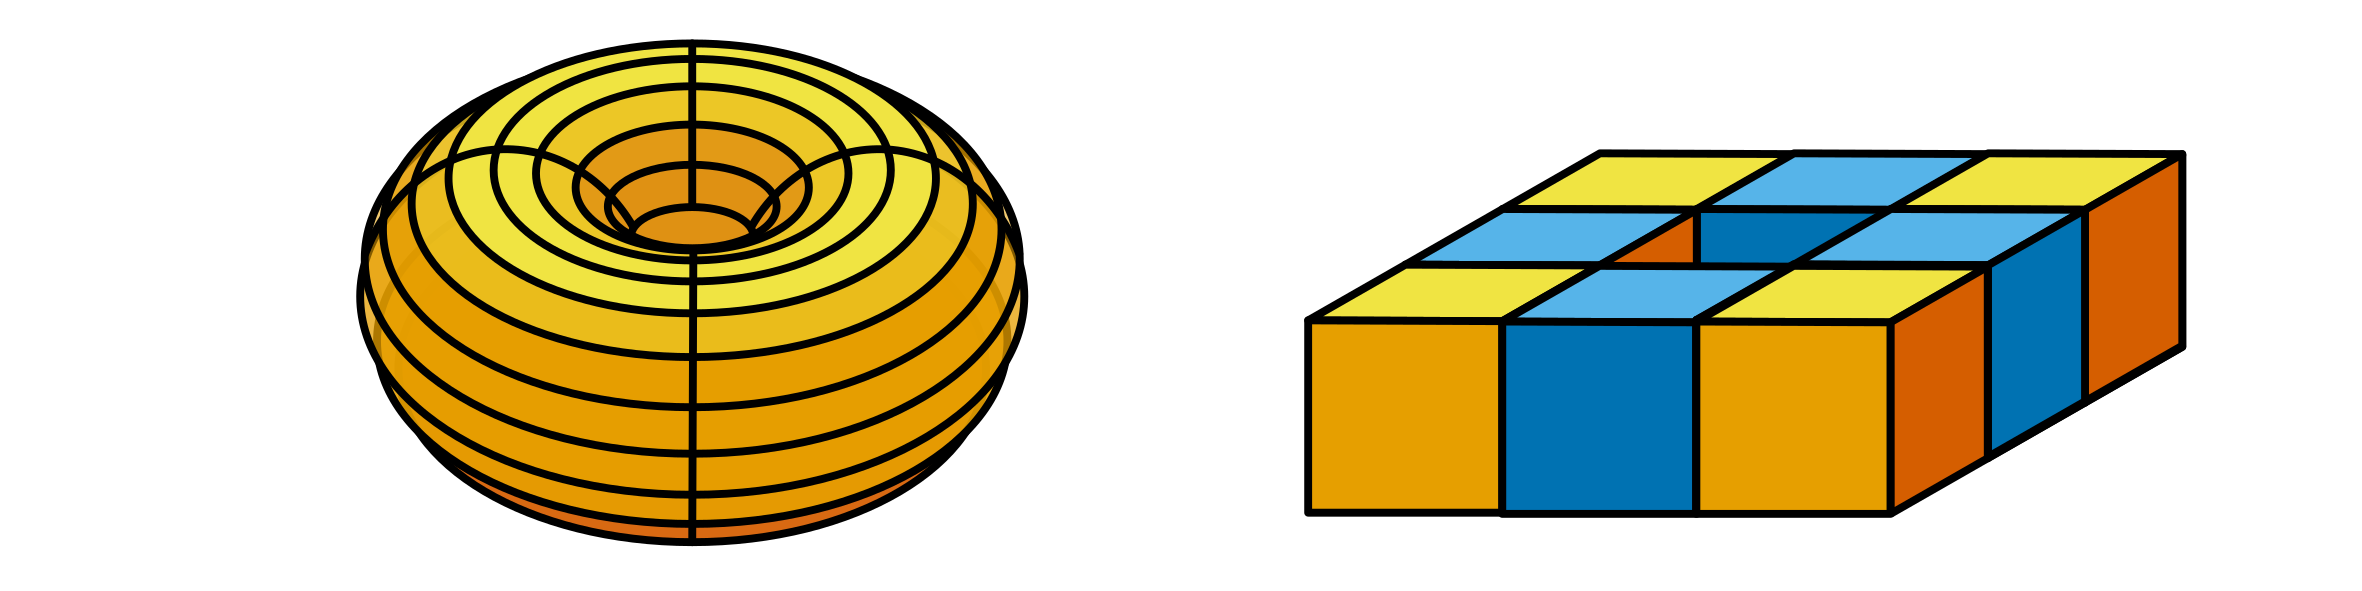
\includegraphics[width=\textwidth]{Figure 7.8.A}
\caption{A checker pattern with a hole has the same Euler characteristic as a torus}
\end{figure}
\noindent
The finite-difference mesh of $S_t$ is given by $T_S = |\Delta S_t|$, assuming we switch to the convention that each cell $x \in \mathbb B_\circ$. The finite-difference mesh of the Boolean field $T_S$ has an Euler characteristic that is \textit{exactly} equal to the Euler characteristic of a truly continuous torus. We say that a graph $G$ may be embedded on a surface $\Sigma$ if we may draw its vertices and edges on that surface.

The \textbf{Heawood conjecture}\index{Heawood conjecture} relates the upper and lower bound of a graph's coloring with respect to its Euler characteristic $\chi$:
$$\mathcal H = \frac{7 \pm \sqrt{49 - 24 \chi}}{2}$$
in which $\mathcal H$ is called the Heawood number. A $k$-chromatic graph can use $k$ independent sets of vertices whose union equals all vertices. An independent set of vertices is a set of vertices that does are not adjacent to each other, or not connected by an edge. We might consider the optimal chromatic number $k$ of a Boolean random walk's finite-difference mesh $T$ to be a rough measure of its (computational) complexity.

Any finite-graph may be embedded in $\mathbb R^3$. Minimal embedding is the tricky part. A graph $G$ has an orientable genus number $n$ (or a non-orientable genus number $m$) if $n$ is the smallest genus surface that may embed $G$. It is not so obvious to determine the genus of a graph. 
\begin{figure}[H]
\centering
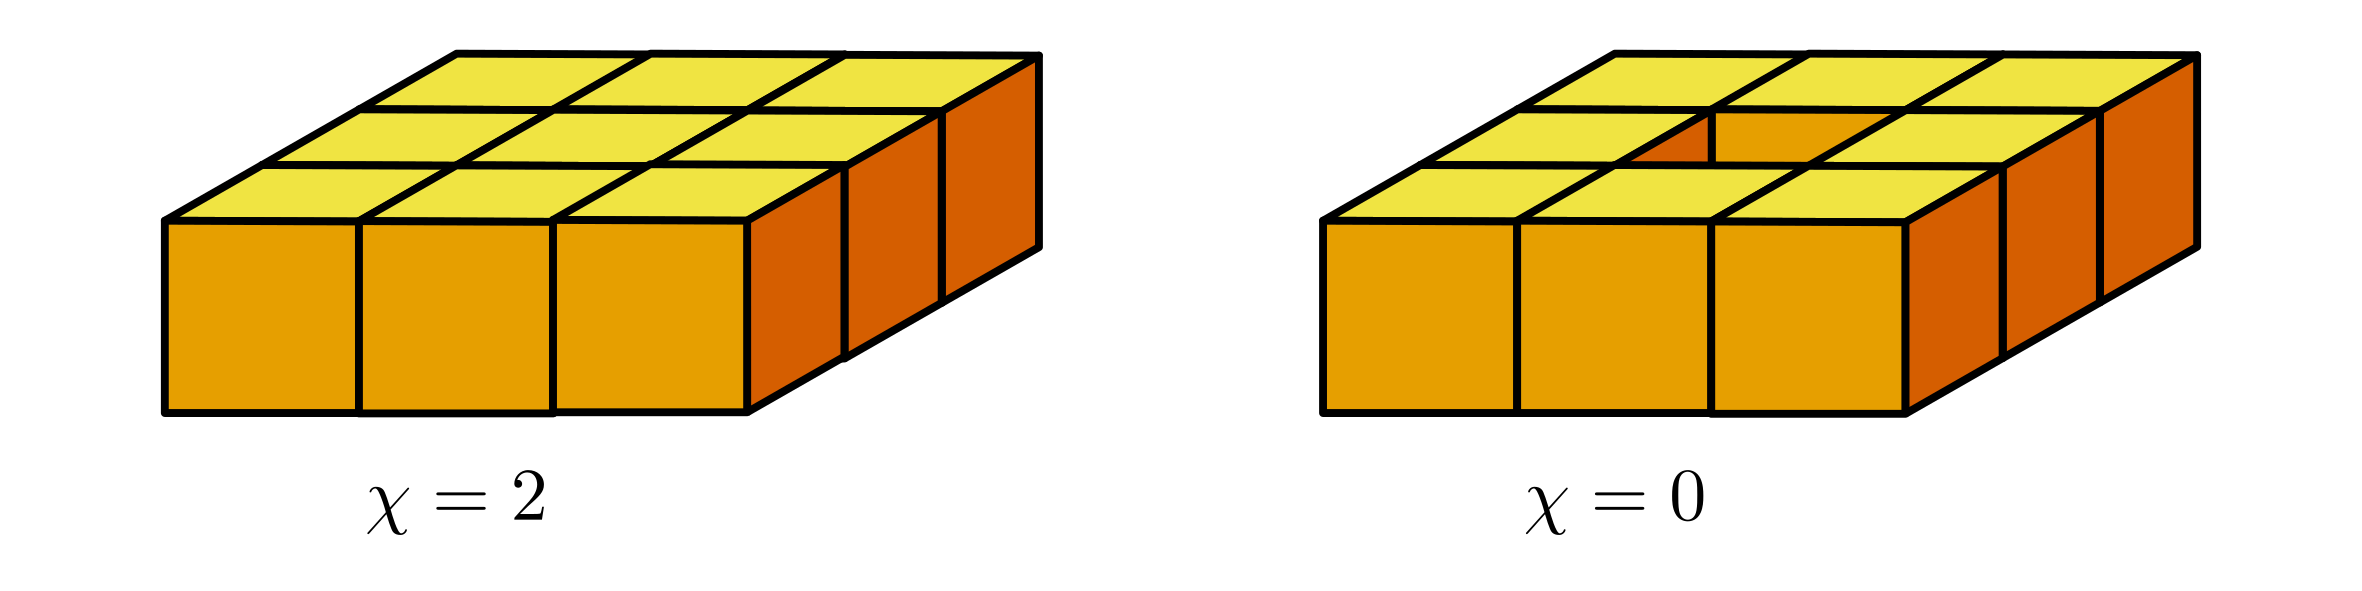
\includegraphics[width=\textwidth]{Figure 7.8.B}
\caption{A torus and cuboid made of smaller cubes have differing $\chi$}
\end{figure}
\noindent In this example, connecting cubes consecutively has the same genus as a single cube. Yet, connecting cubes into a loop does not share the genus of a cube. An orientable surface has a genus number of $n$ from $\chi = 2 - 2n$. A non-orientable surface has a genus number of $m$ from $\chi = 2 - m$.

Elliptic curves are used in cryptography for the secure transmission of information. In terms of topology, an elliptic curve is the embedding of a torus on the complex projective plane: 
$$(x_1, x_2, x_3) \in \mathbb C, \quad (x_1, x_2, x_3) \neq (0,0,0)$$
with a constant period of $p \in \mathbb C, \ p \neq 0$ such that:
$$(x_1, x_2, x_3) \equiv (p x_1,p x_2, p x_3) = p(x_1, x_2, x_3) $$
The complex manifold that the encrypting function rotates around is of dimension $2$. This the reason why I assert that macroparticles in Boolean random walks are related to cryptography and topological defects. If the eigenvalue $\lambda$ of a transition matrix $P$ has a magnitude near $1$ and a period $\omega^{-1}$ that is almost exactly a natural number:
$$\mu \approx 1$$
$$\omega^{-1} \approx n, \ n \in \mathbb N$$
then the state space graph of that transition matrix can be embedded on a complex manifold $\Sigma$ with period $\omega^{-1}$. This manifold represents a non-decaying periodic system with different phases, and it implicitly preserves some measure such as energy. This is exactly what we anticipate from the phase space of a particle, a periodic phenomenon.

\section{Topological Defects}
A \textbf{topological defect}\index{topological defect} in a crystalline lattice is any imperfection or dislocation in the lattice's regular structure. A crystal lattice is $d$-regular if each vertex is of degree $d$, meaning the vertex has $d$ edges connected to it. Plastic deformation is the result of the creation and relocation of these dislocations. Suppose you have a sequence of instructions that forms a closed loop on the regular lattice, such as a plaquette on a rectangular lattice. That sequence of instructions will fail to close around a defect.

\textbf{Edge dislocations}\index{edge dislocation} refer to vertices with reduced degree of connectivity. Since a vertex has less edges connected, a sequence of instructions to form a closed loop may fail because the edge to traverse does not exist.
\begin{figure}[H]
\centering
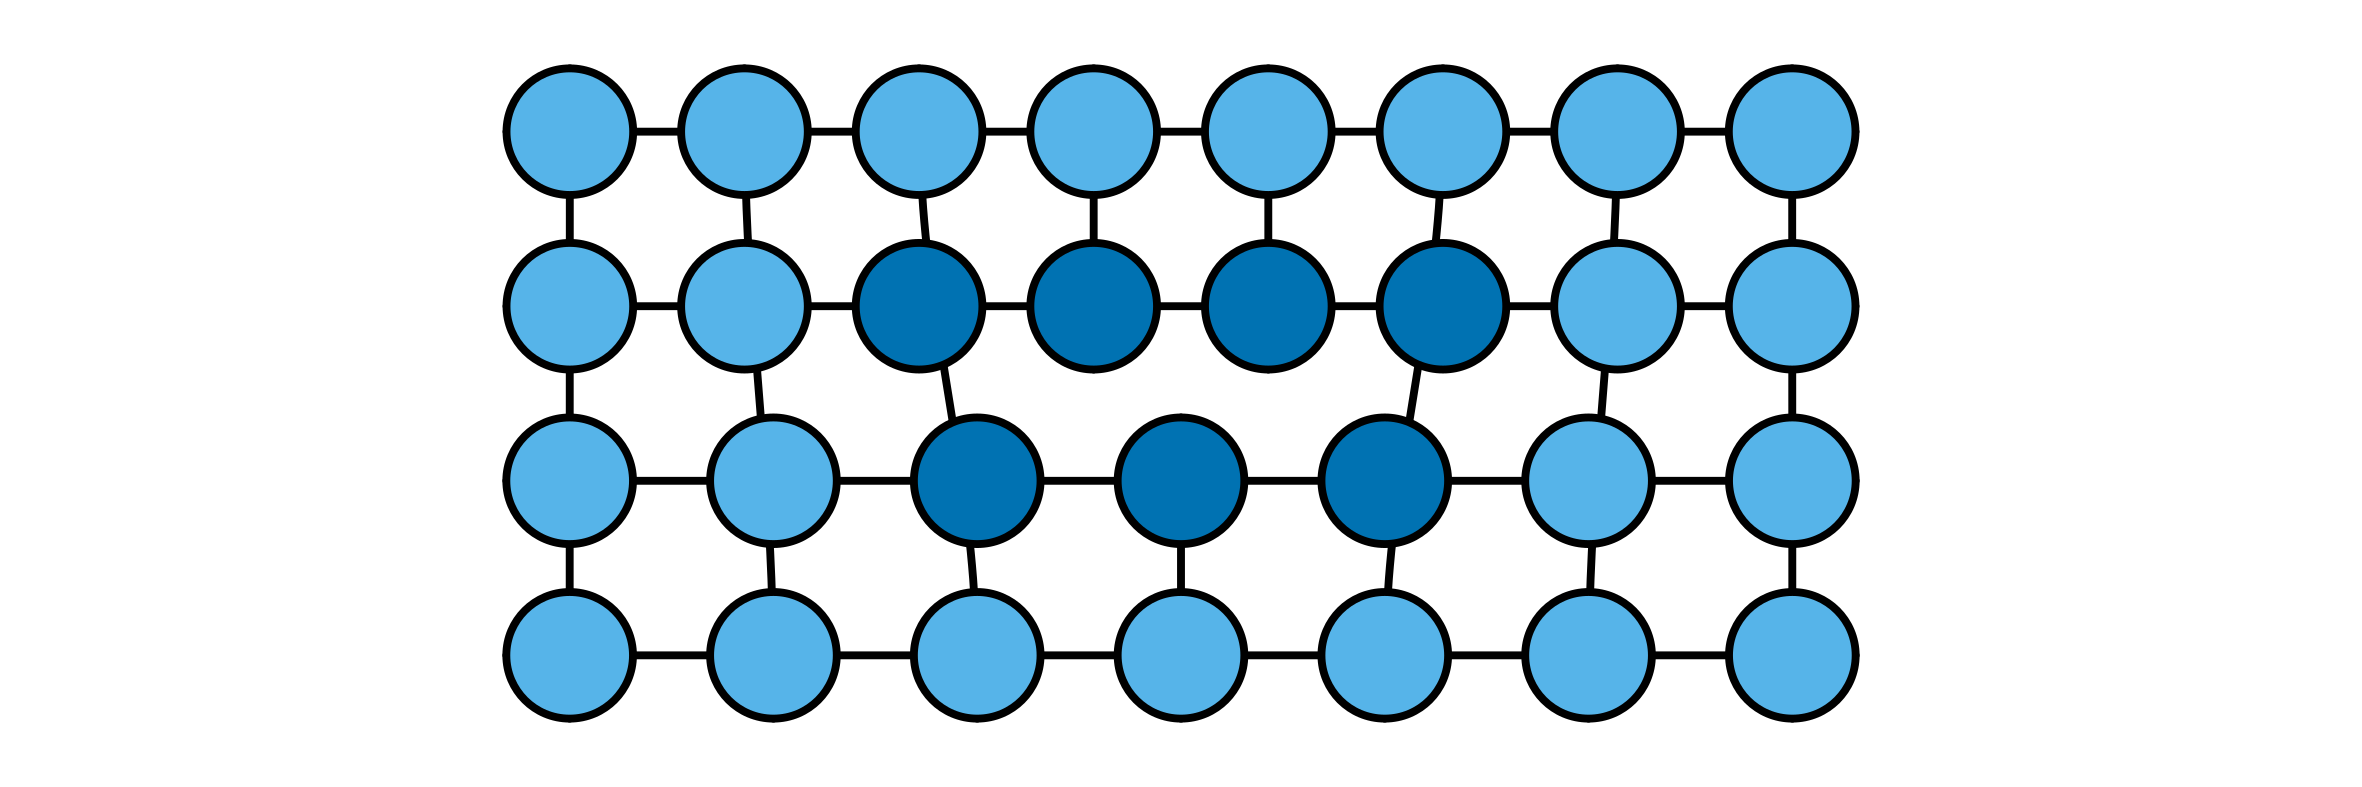
\includegraphics[width=\textwidth]{Figure 7.9.A}
\caption{An edge dislocation caused by a missing edge}
\end{figure}
\textbf{Screw dislocations}\index{screw dislocation} refer to slipping or skipping in the connections between vertices. Since a vertex has an edge that does not connect to the usual place, a sequence of instructions to form a closed loop may fail because it overshoots or undershoots its origin.
\begin{figure}[H]
\centering
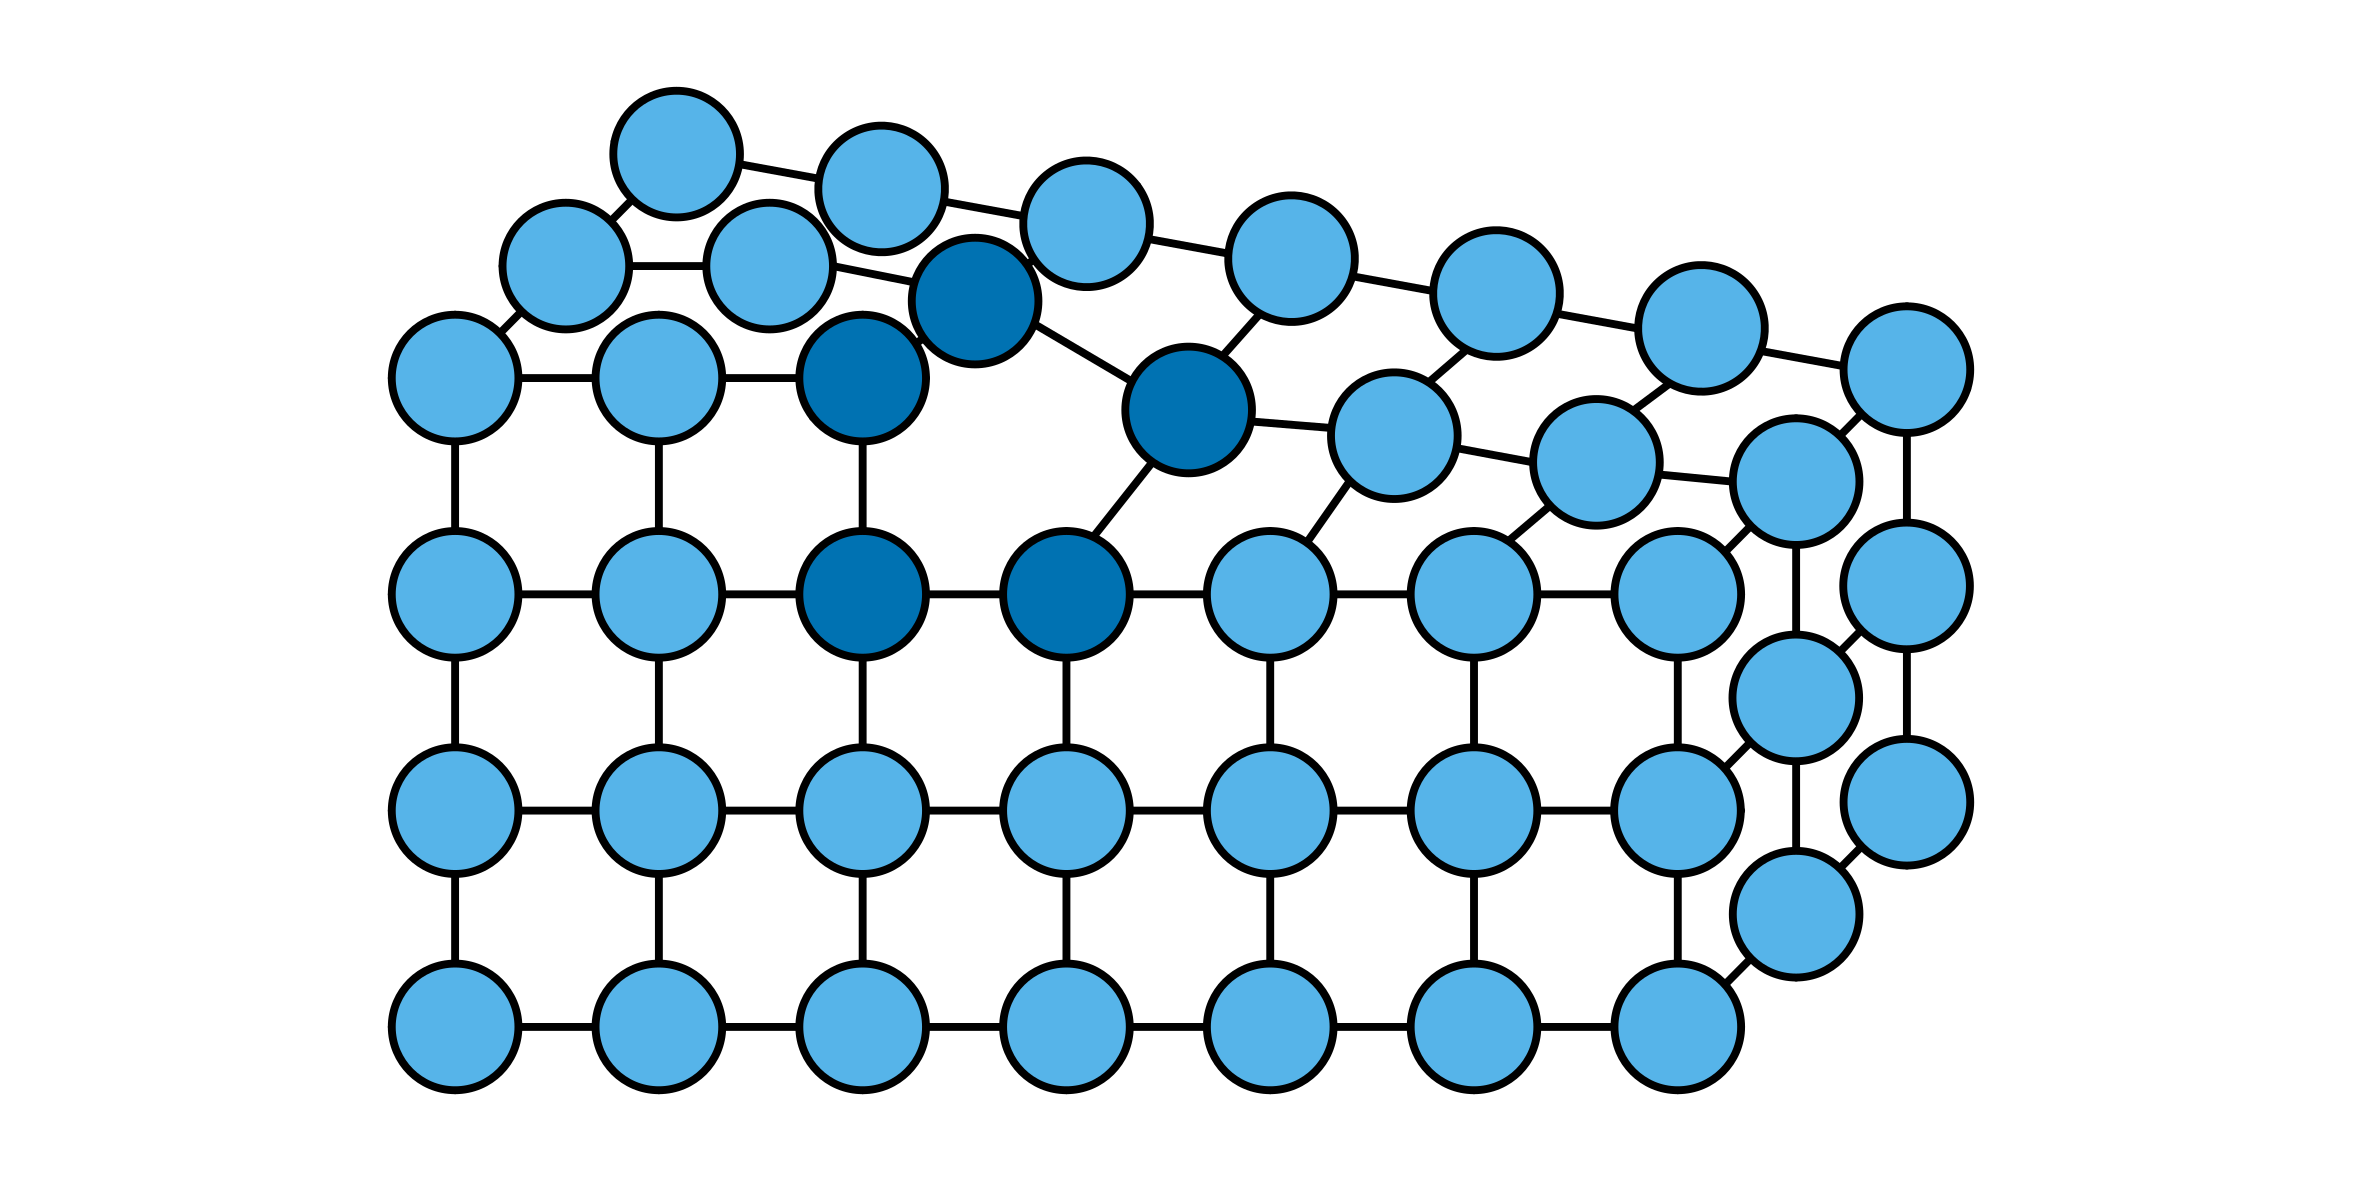
\includegraphics[width=\textwidth]{Figure 7.9.B}
\caption{A screw dislocation caused by accumulated angle error}
\end{figure}

Screw dislocations in a crystalline material are topological defects. If that crystalline material evolves according to a differential equation, then that topological defect is a topological soliton. We cannot smoothly deform the topology of the crystal into the uniform lattice to erase the soliton. A soliton is a self-stabilizing wave packet:
\begin{figure}[H]
\centering
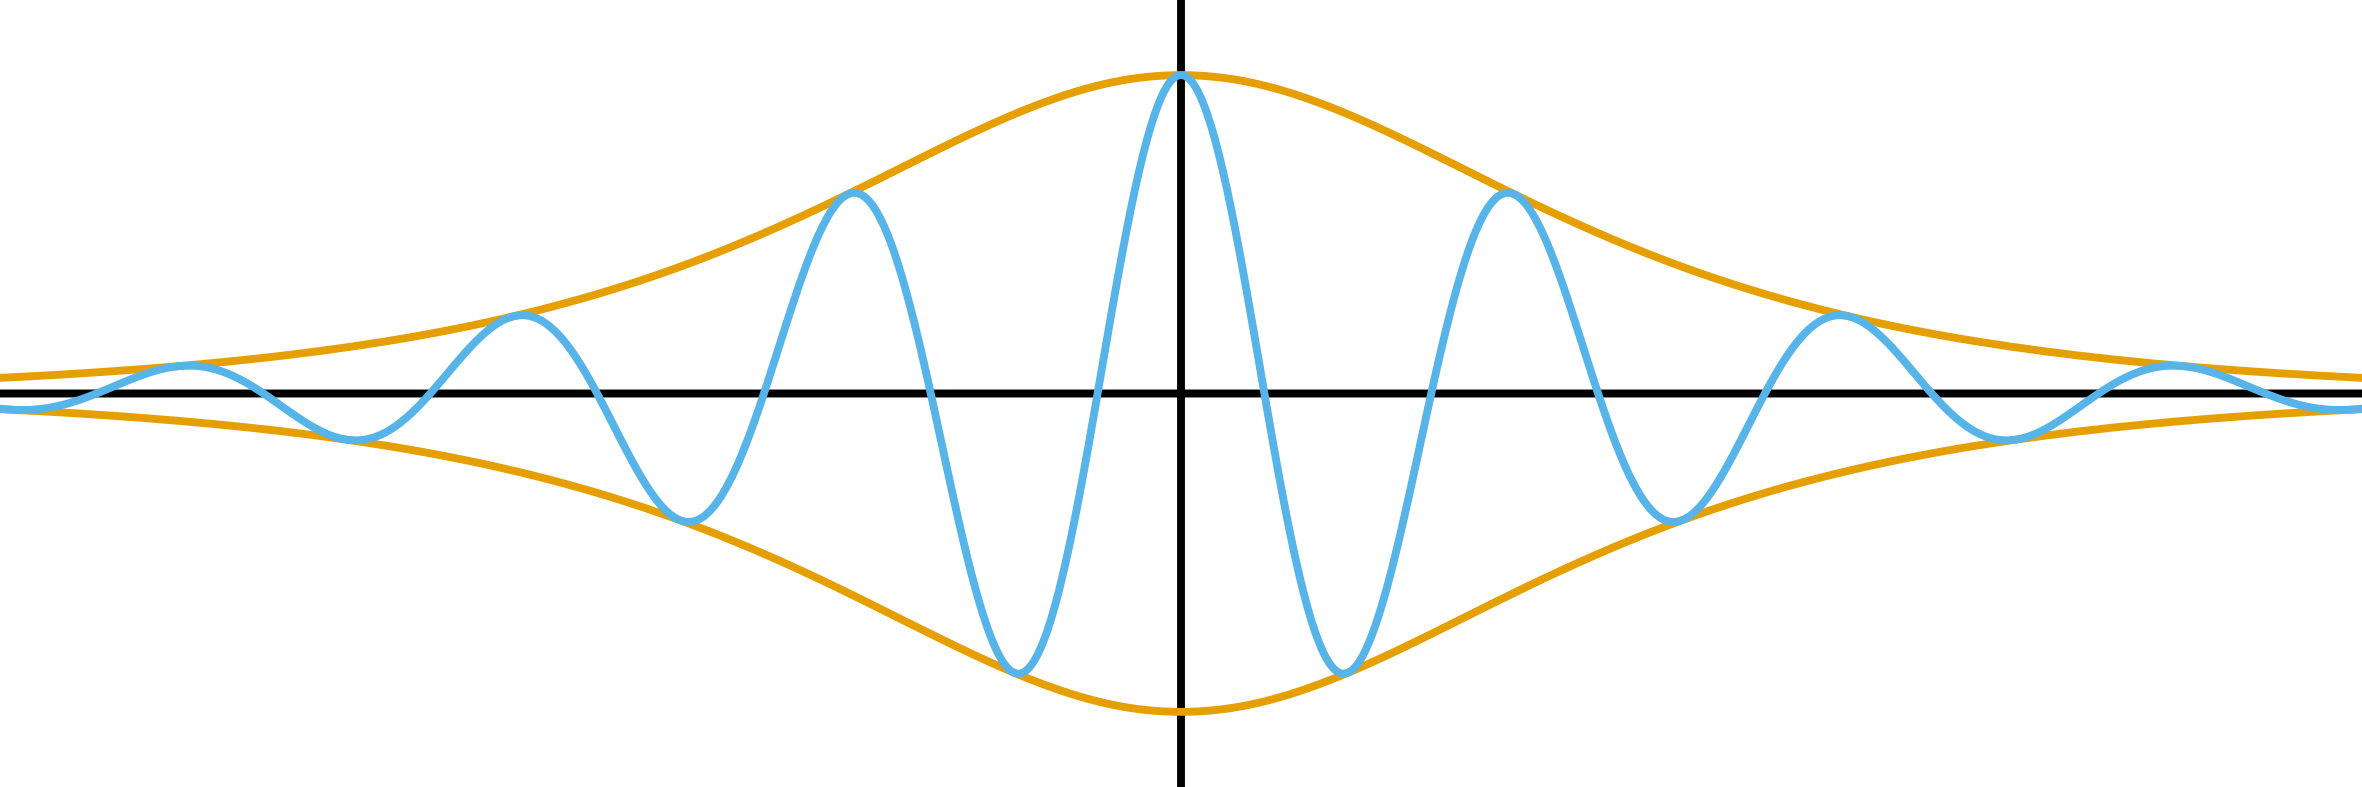
\includegraphics[width=\textwidth]{Figure 7.9.C}
\caption{A soliton is self-stabilizing shape that cannot smoothly deform to zero}
\end{figure}
\noindent 
This is an example of a wave packet with an envelope of $\textnormal{sech}(x)$ and $-\textnormal{sech}(x)$. There is something special about their potential energy function $V$ or their Hamiltonian energy function $H$ that results in spatiotemporal stability. We discuss more about solitons in \textit{\S 11.7 Macroparticle Creation and Annihilation} and more about potential wells in \textit{\S 11.4 Boolean Heat Equation}.

A large amount of water particles will approximate a continuum. Self-stabilizing waves occur in water due to the particles and forces, vertices and edges respectively, having dislocations in their topology. For the self-stabilizing wave to disappear, the wave must experience an abrupt topological change. Of course, a dislocation may appear and disappear more freely in a Boolean random walk simulation because it does not need to obey smooth deformation of graphs. 

\section{Stokes Theorem on Graphs}
For the problem of 3D Boolean random walks, we define the \textbf{pseudo-curl}\index{pseudo-curl} $\psi \kappa$ in the following way. If we are interested in the curl for $x_1$, then we need something representing the bivector for $(x_2, x_3)$ in that order. Just like regular curl, the bivector for $(x_3, x_2)$ is equal to the negative of the bivector for $(x_2, x_3)$. Let us take what we have learned here to state the definition of pseudo-curl about $x_1$ for a discrete vector field $H$ for a Boolean random walk:\footnote{We are assuming $H$ to be the expected transition probabilities along the finite-difference graph $T$.}
$$\psi \kappa (x_1) \times H = 
e^{+\frac{\partial}{\partial x_3}} f[H_{x_2} - H_{x_{-2}}] 
-e^{+\frac{\partial}{\partial x_2}} f[H_{x_3} - H_{x_{-3}}]
$$
$$
-e^{-\frac{\partial}{\partial x_3}} f[H_{x_2} - H_{x_{-2}}]
+e^{-\frac{\partial}{\partial x_2}} f[H_{x_3} - H_{x_{-3}}]
$$
The pseudo-curl about $x_2$ for $H$ likewise given by:
$$\psi \kappa (x_2) \times H = 
e^{+\frac{\partial}{\partial x_1}} f[H_{x_3} - H_{x_{-3}}] 
-e^{+\frac{\partial}{\partial x_3}} f[H_{x_1} - H_{x_{-1}}]
$$
$$
-e^{-\frac{\partial}{\partial x_1}} f[H_{x_3} - H_{x_{-3}}]
+e^{-\frac{\partial}{\partial x_3}} f[H_{x_1} - H_{x_{-1}}]
$$
The pseudo-curl about $x_3$ for $H$ is likewise given by:
$$\psi \kappa (x_3) \times H = 
e^{+\frac{\partial}{\partial x_2}} f[H_{x_1} - H_{x_{-1}}] 
-e^{+\frac{\partial}{\partial x_1}} f[H_{x_2} - H_{x_{-2}}]
$$
$$
-e^{-\frac{\partial}{\partial x_2}} f[H_{x_1} - H_{x_{-1}}]
+e^{-\frac{\partial}{\partial x_1}} f[H_{x_2} - H_{x_{-2}}]
$$
These formulas are a quite cumbersome when observed without context. What do these formulas mean? What does each added term of the formula represent?

We define $f$ as the Boolean value of the cell, $\mathbb B_\pm = \{-1, +1\}$. We define $e^{\frac{\partial}{\partial x_i}}$ as the shift operator along dimension $x_i$. We therefore define $e^{c\frac{\partial}{\partial x_i}} f$ as extracting the value of $f$ that is $c$ units along dimensions $x_i$. We define $H_{x_i}$ as the Hamiltonian probability in the forward direction of a cell $f$, also known as the probability of making a bit flip in the forward direction. This means that the backwards Hamiltonian probability is given by the identity:
$$f( H_{x_{-2}}) = f(e^{\frac{-\partial}{\partial x_2}} H_{x_2})$$
We shall abuse notation and say that:
$$f[H_{x_i} - H_{x_{-i}}]$$
is the Hamiltonian probabilities multiplied by the Boolean value of the cell. This assigns a ``magnetic orientation'' to the curl. Thus we define:
$$e^{c \frac{\partial}{\partial x_j}} f[H_{x_i} - H_{x_{-i}}]$$
as the forwards minus backwards switch probability of the shifted cell, all multiplied by its Boolean parity.

The advantage of pseudo-curl over regular curl is that we can define magnetism for a single cell instead of a plaquette of four cells.\footnote{Statistical mechanics on lattices often uses curl to define magnetism on a plaquette of four cells. The weakness of plaquettes is that magnetism is no longer centered on the cell, but using four plaquettes about the cell is exactly pseudo-curl.} This can succinctly be summarized in the following image:
\begin{figure}[H]
\centering
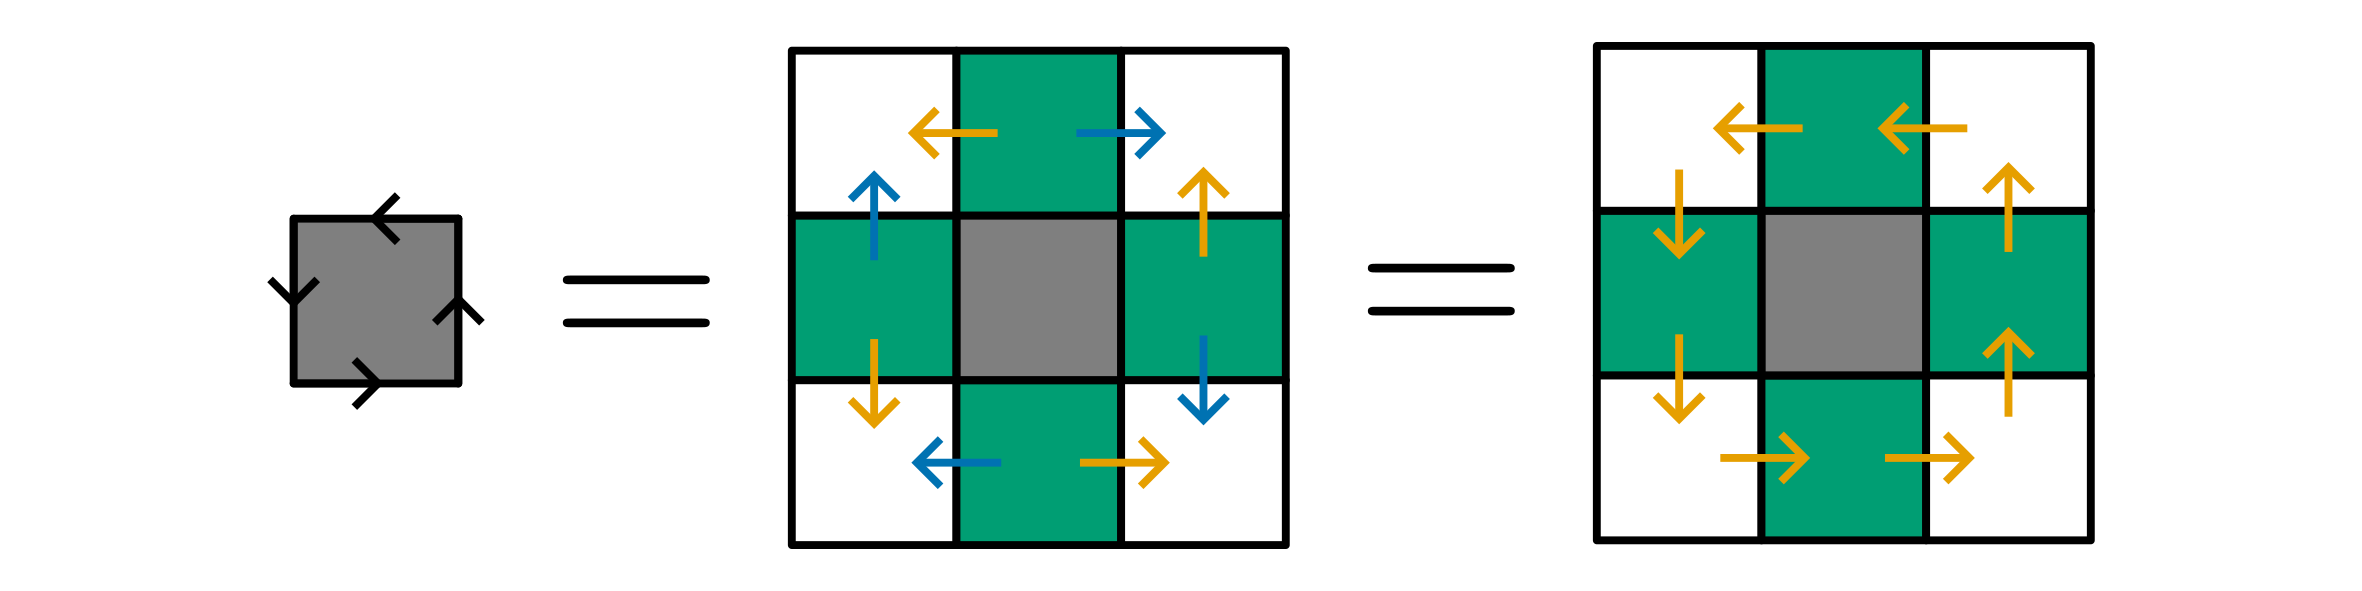
\includegraphics[width=\textwidth]{Figure 7.10.A}
\caption{We measure the flow perpendicular to adjacent cells, and negative flow in the opposing direction is positive flow in the standard direction}
\end{figure}
\noindent
In this image, the four cells adjacent to center cell have forwards and backwards switches perpendicular to the shift. There is no agreed consensus of discrete curl on cubic lattices that keeps measures isotropic, particularly with respect to diagonals. 

Why do we need a definition of curl for Boolean random walks? Consider a magnetic gear with six teeth, in which three are positively charged and three are negatively charged.
\begin{figure}[H]
\centering
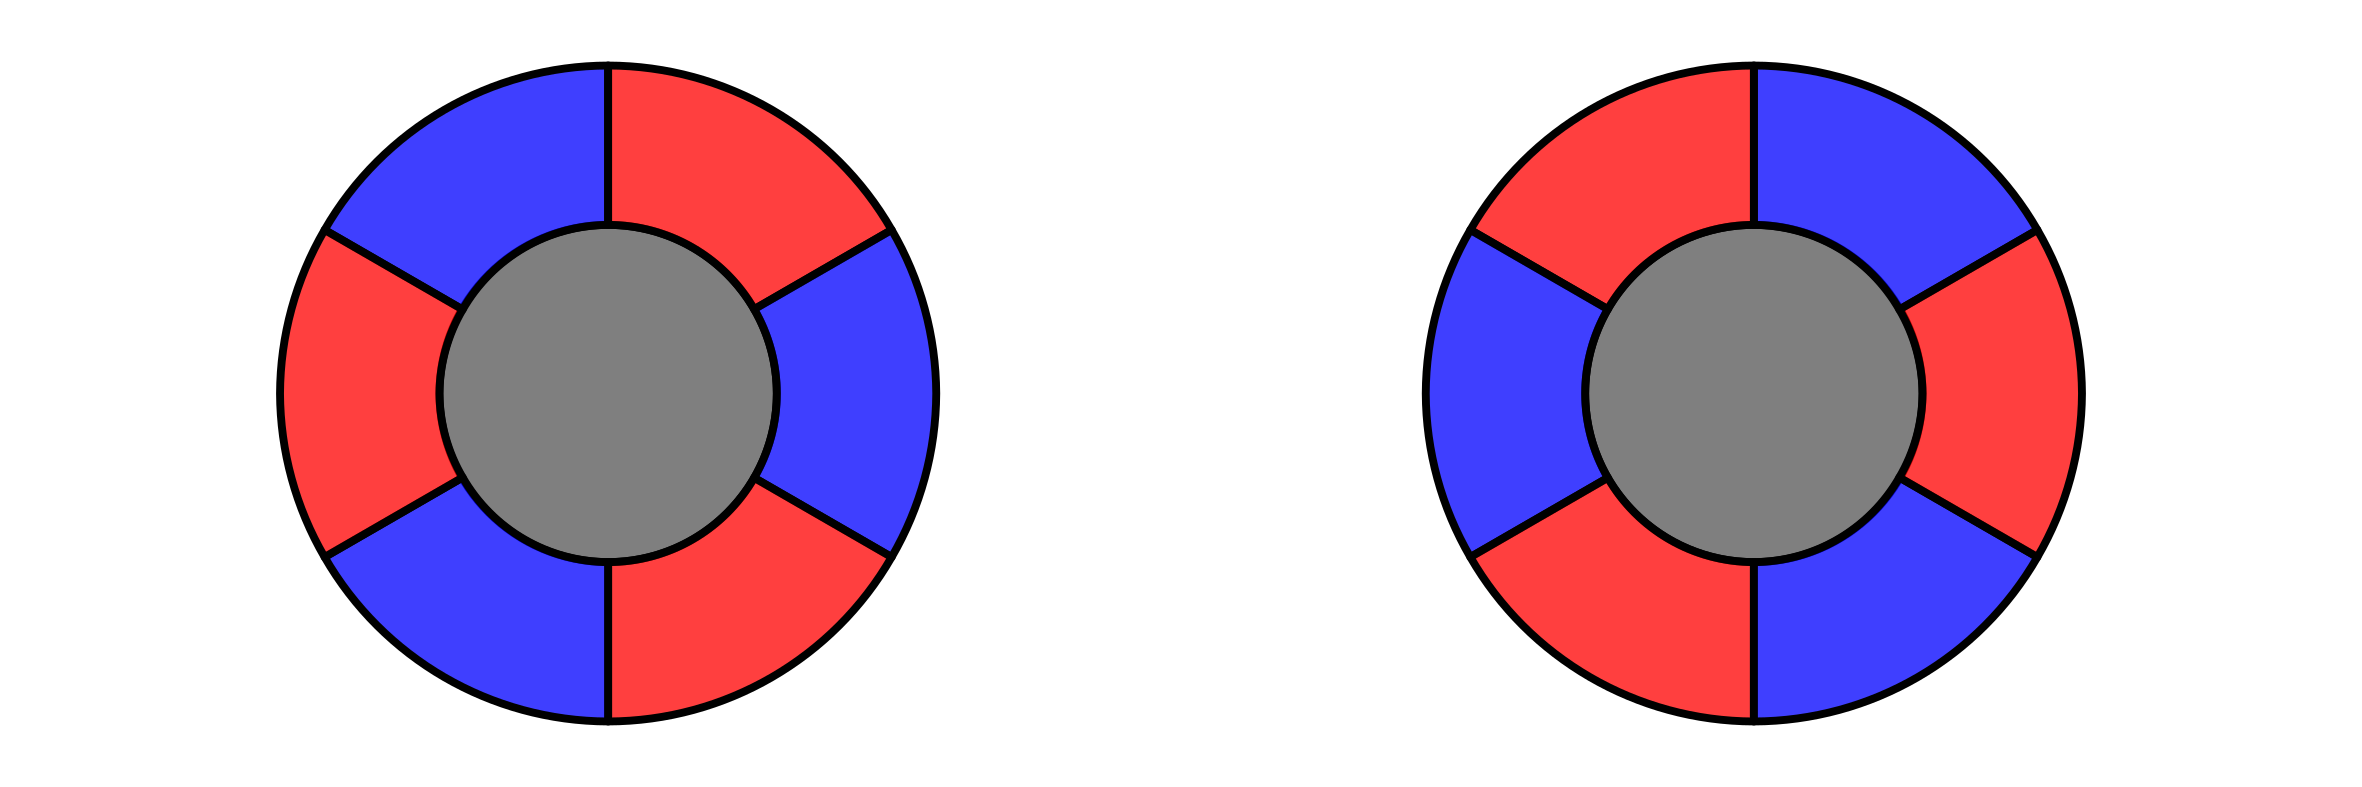
\includegraphics[width=\textwidth]{Figure 7.10.B}
\caption{The curl of a magnetic gear is ambiguous in discrete time frames but ``obvious'' in continuous time rotations}
\end{figure}
\noindent
In a continuous-time system, the magnetic field changes with the infinitesimal movement of the gear. We can define the momentum of the magnetic field in terms of the movement of positive field, colored red.


Consider a discrete-time 2D Boolean random walk on a hexagonal lattice. We are constraining the problem to a honeycomb of six cells surrounding a center cell.
\begin{figure}[H]
\centering
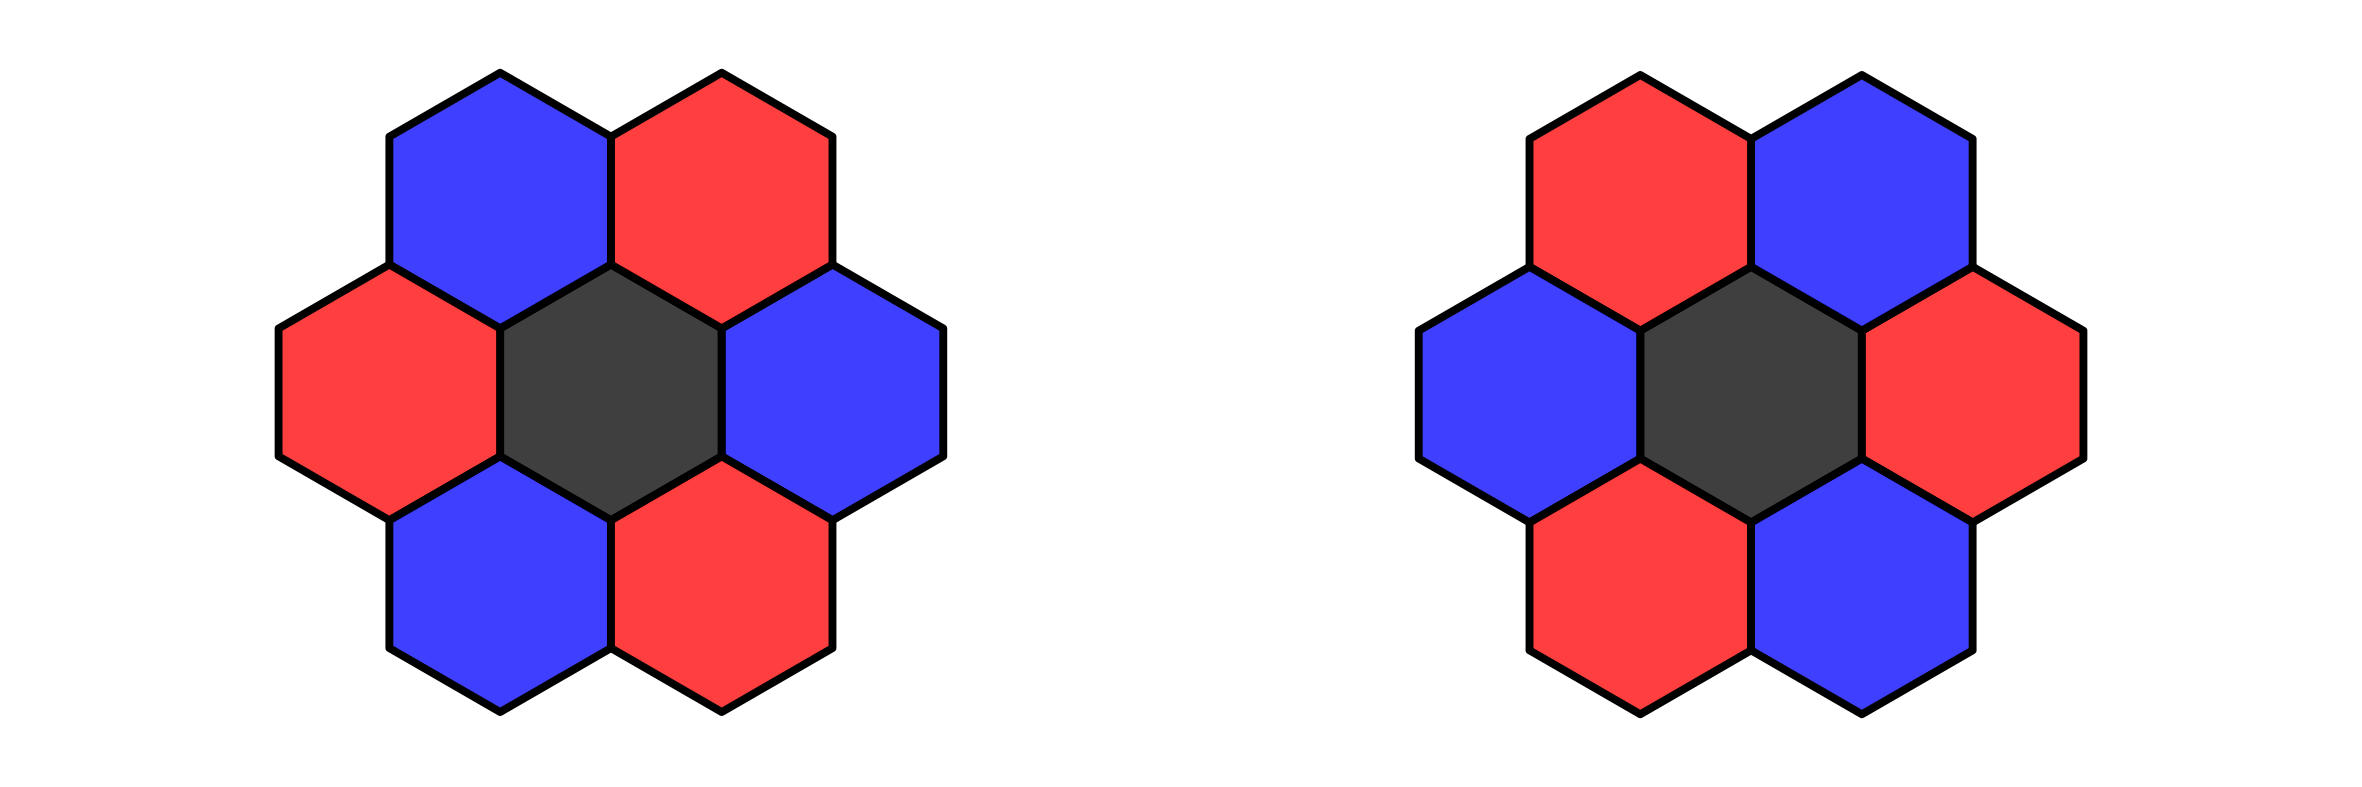
\includegraphics[width=\textwidth]{Figure 7.10.C}
\caption{The curl of random walk in a hexagonal lattice's checker chain is ambiguous}
\end{figure}
\noindent
Which way is the Boolean random walk ``flowing''? We say that a bit flip in one direction is positive and negative in the other.
\begin{figure}[H]
\centering
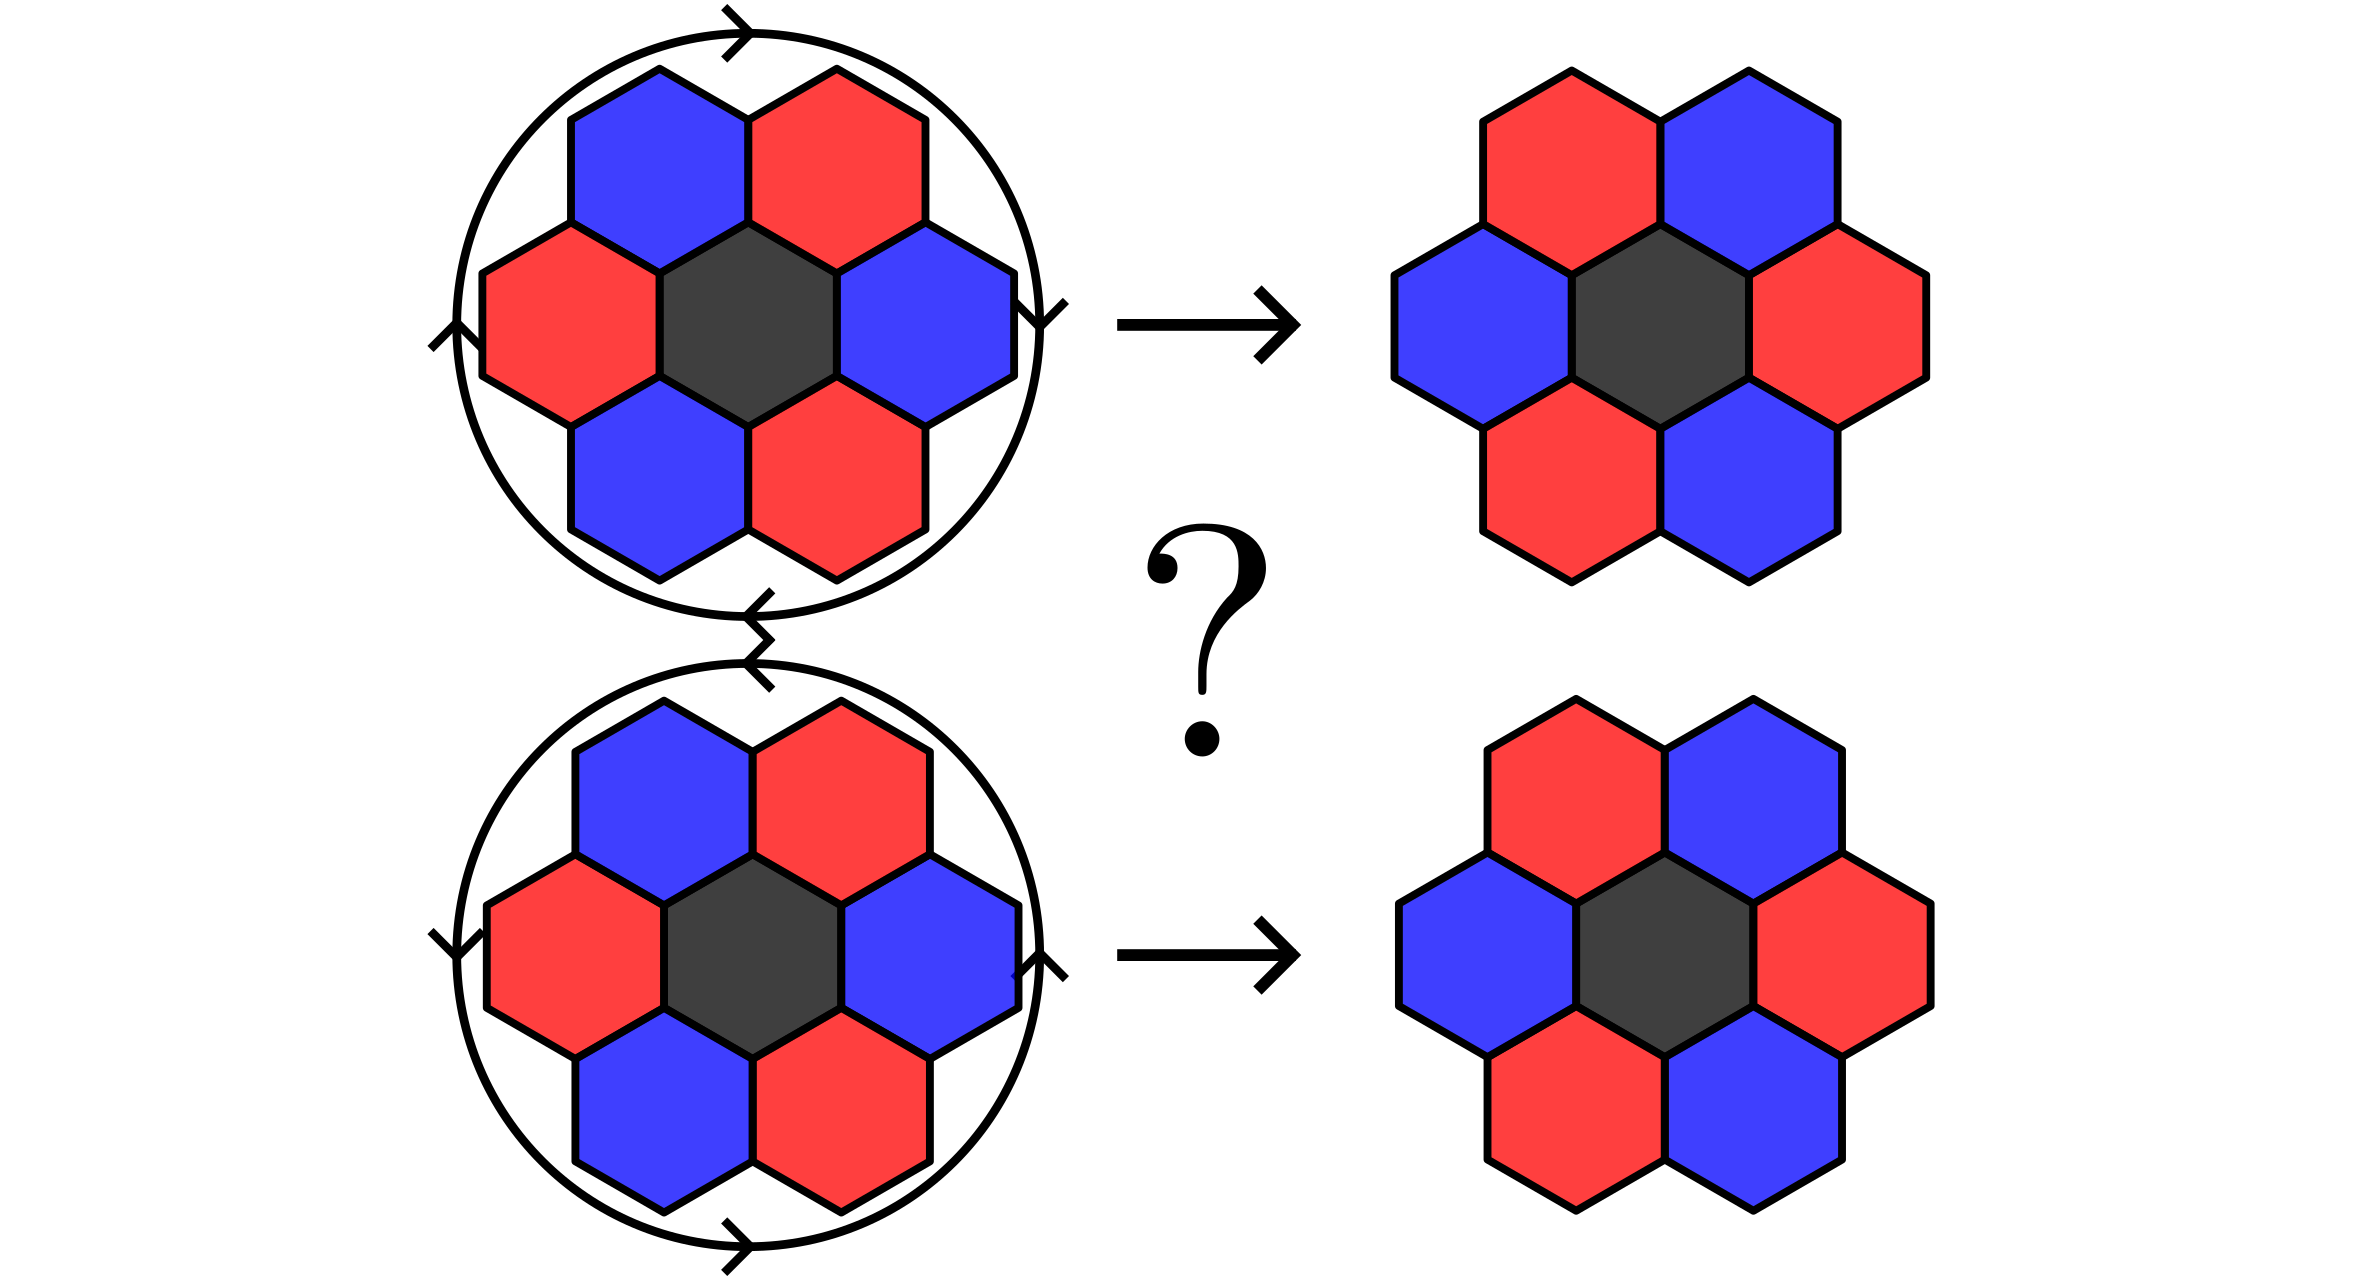
\includegraphics[width=\textwidth]{Figure 7.10.D}
\caption{Ambiguity in rotation direction in a hexagonal lattice}
\end{figure}
\noindent Even still, how can we justify the necessity of our definition of pseudo-curl?

Consider two sparse Boolean random walk in which one is sparse in particles and the other which is sparse in antiparticles. The first field is called $f(x,t)$ and its Boolean inverse is $g(x,t) = -f(x,t)$:
\begin{figure}[H]
\centering
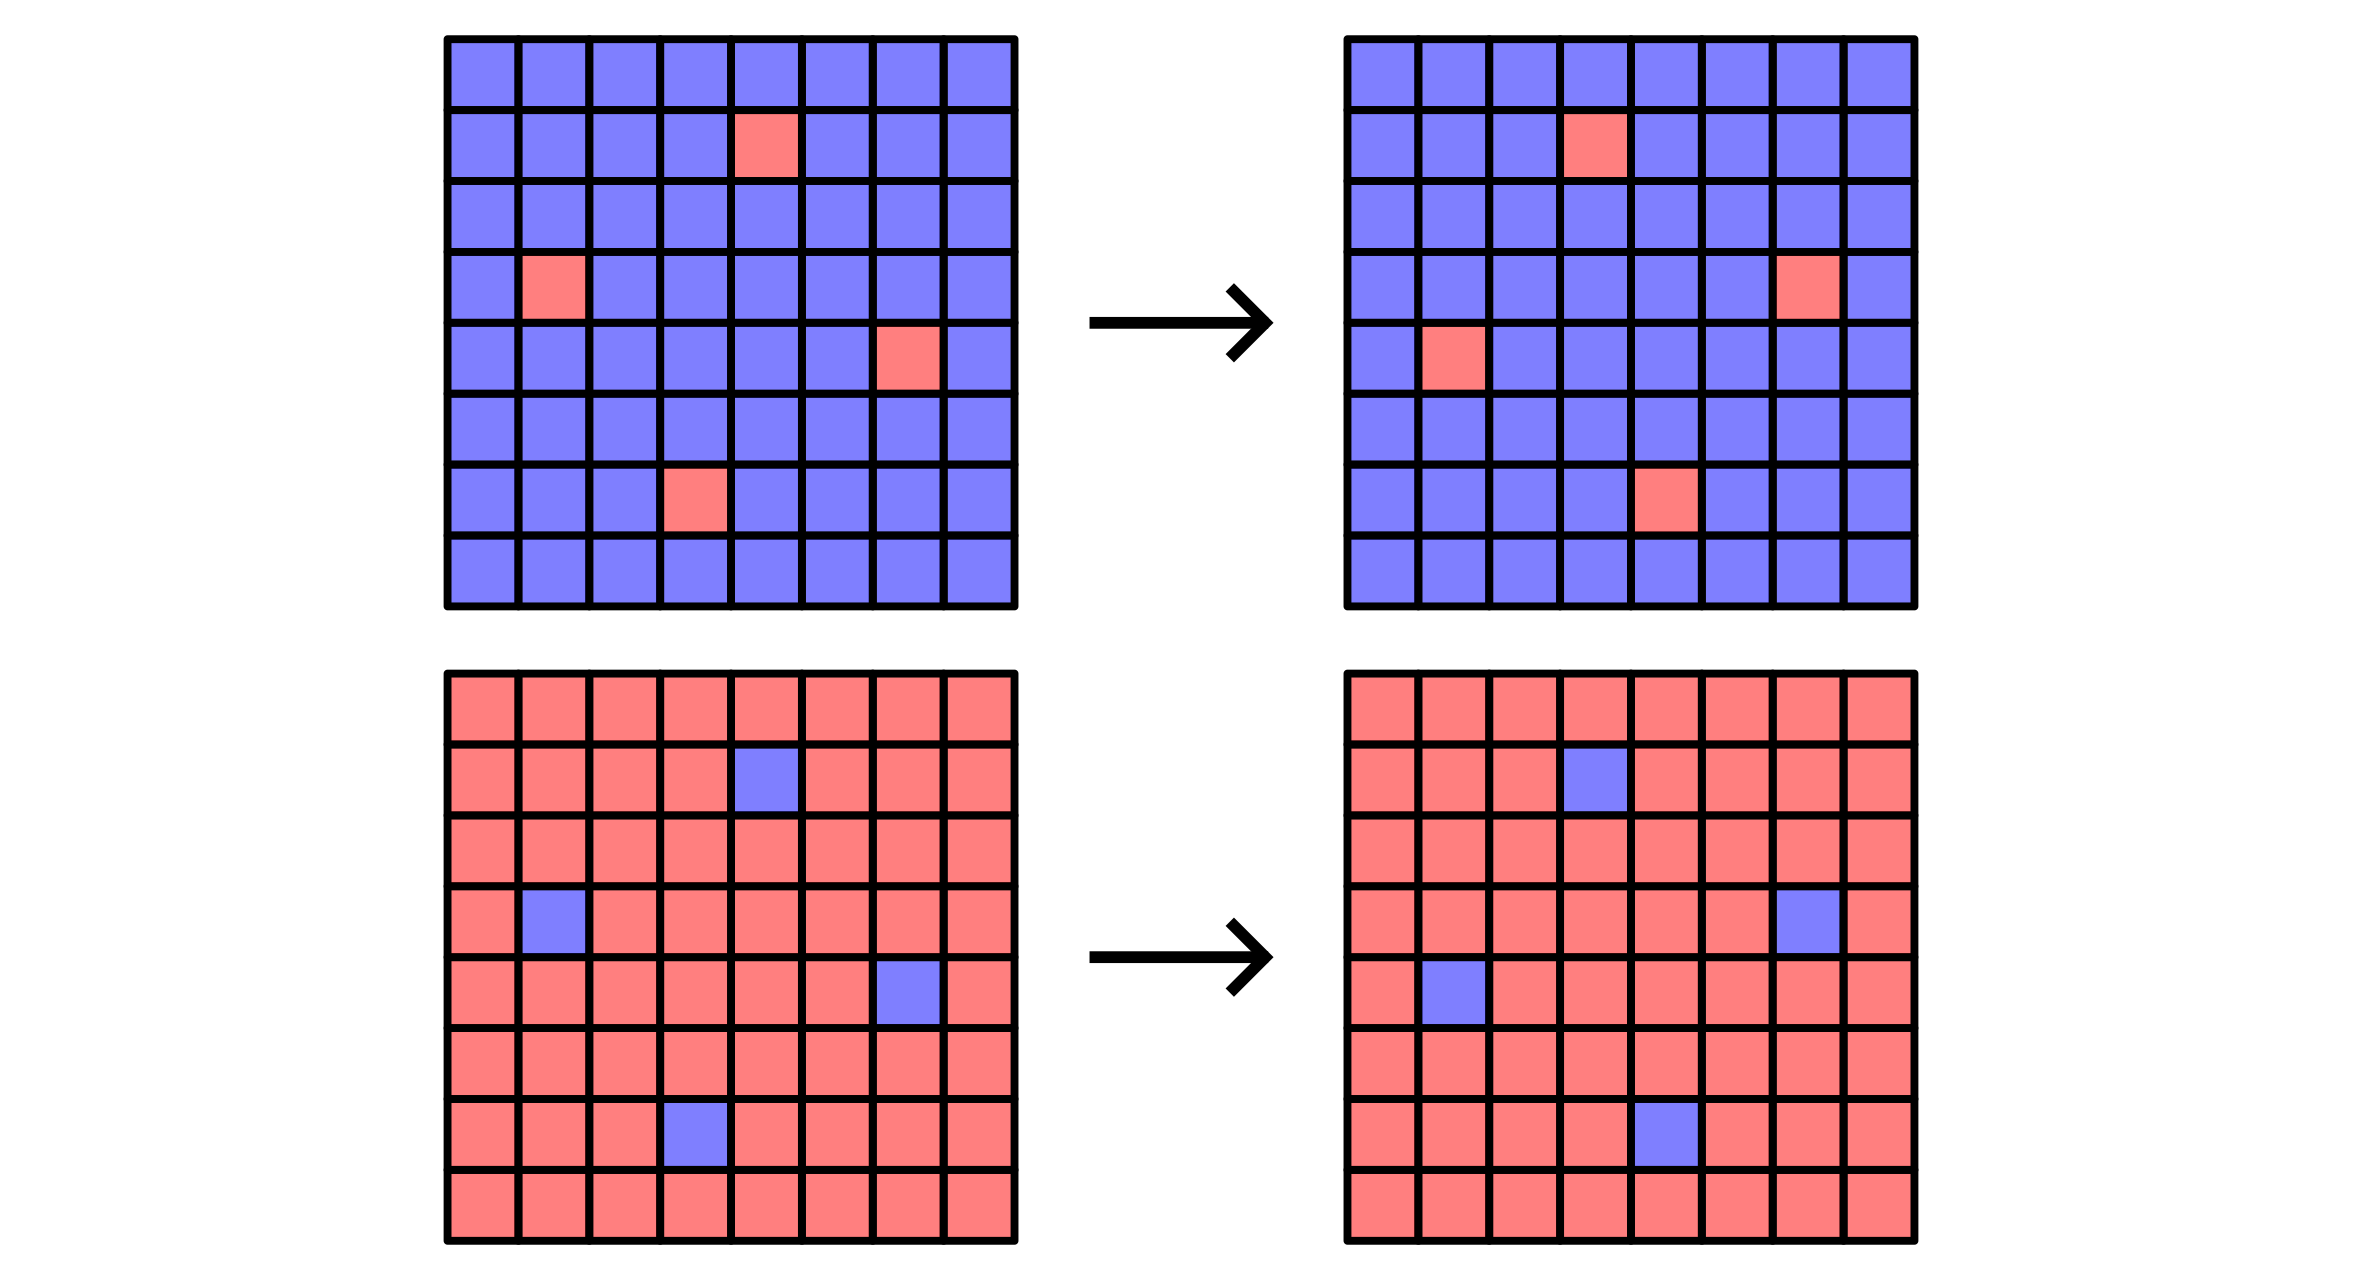
\includegraphics[width=\textwidth]{Figure 7.10.E}
\caption{Ambiguity in rotation ``direction'' for a Boolean random walk}
\end{figure}
\noindent 
We may say that a specific evolution has resulted in counter-clockwise rotation of the $f$ in the positive direction. What can we say about the rotation for $g$? 

In the magnetic gear example, we could see the movement of the minima and the maxima of the magnetic field. Here we have no such option. 
\begin{figure}[H]
\centering
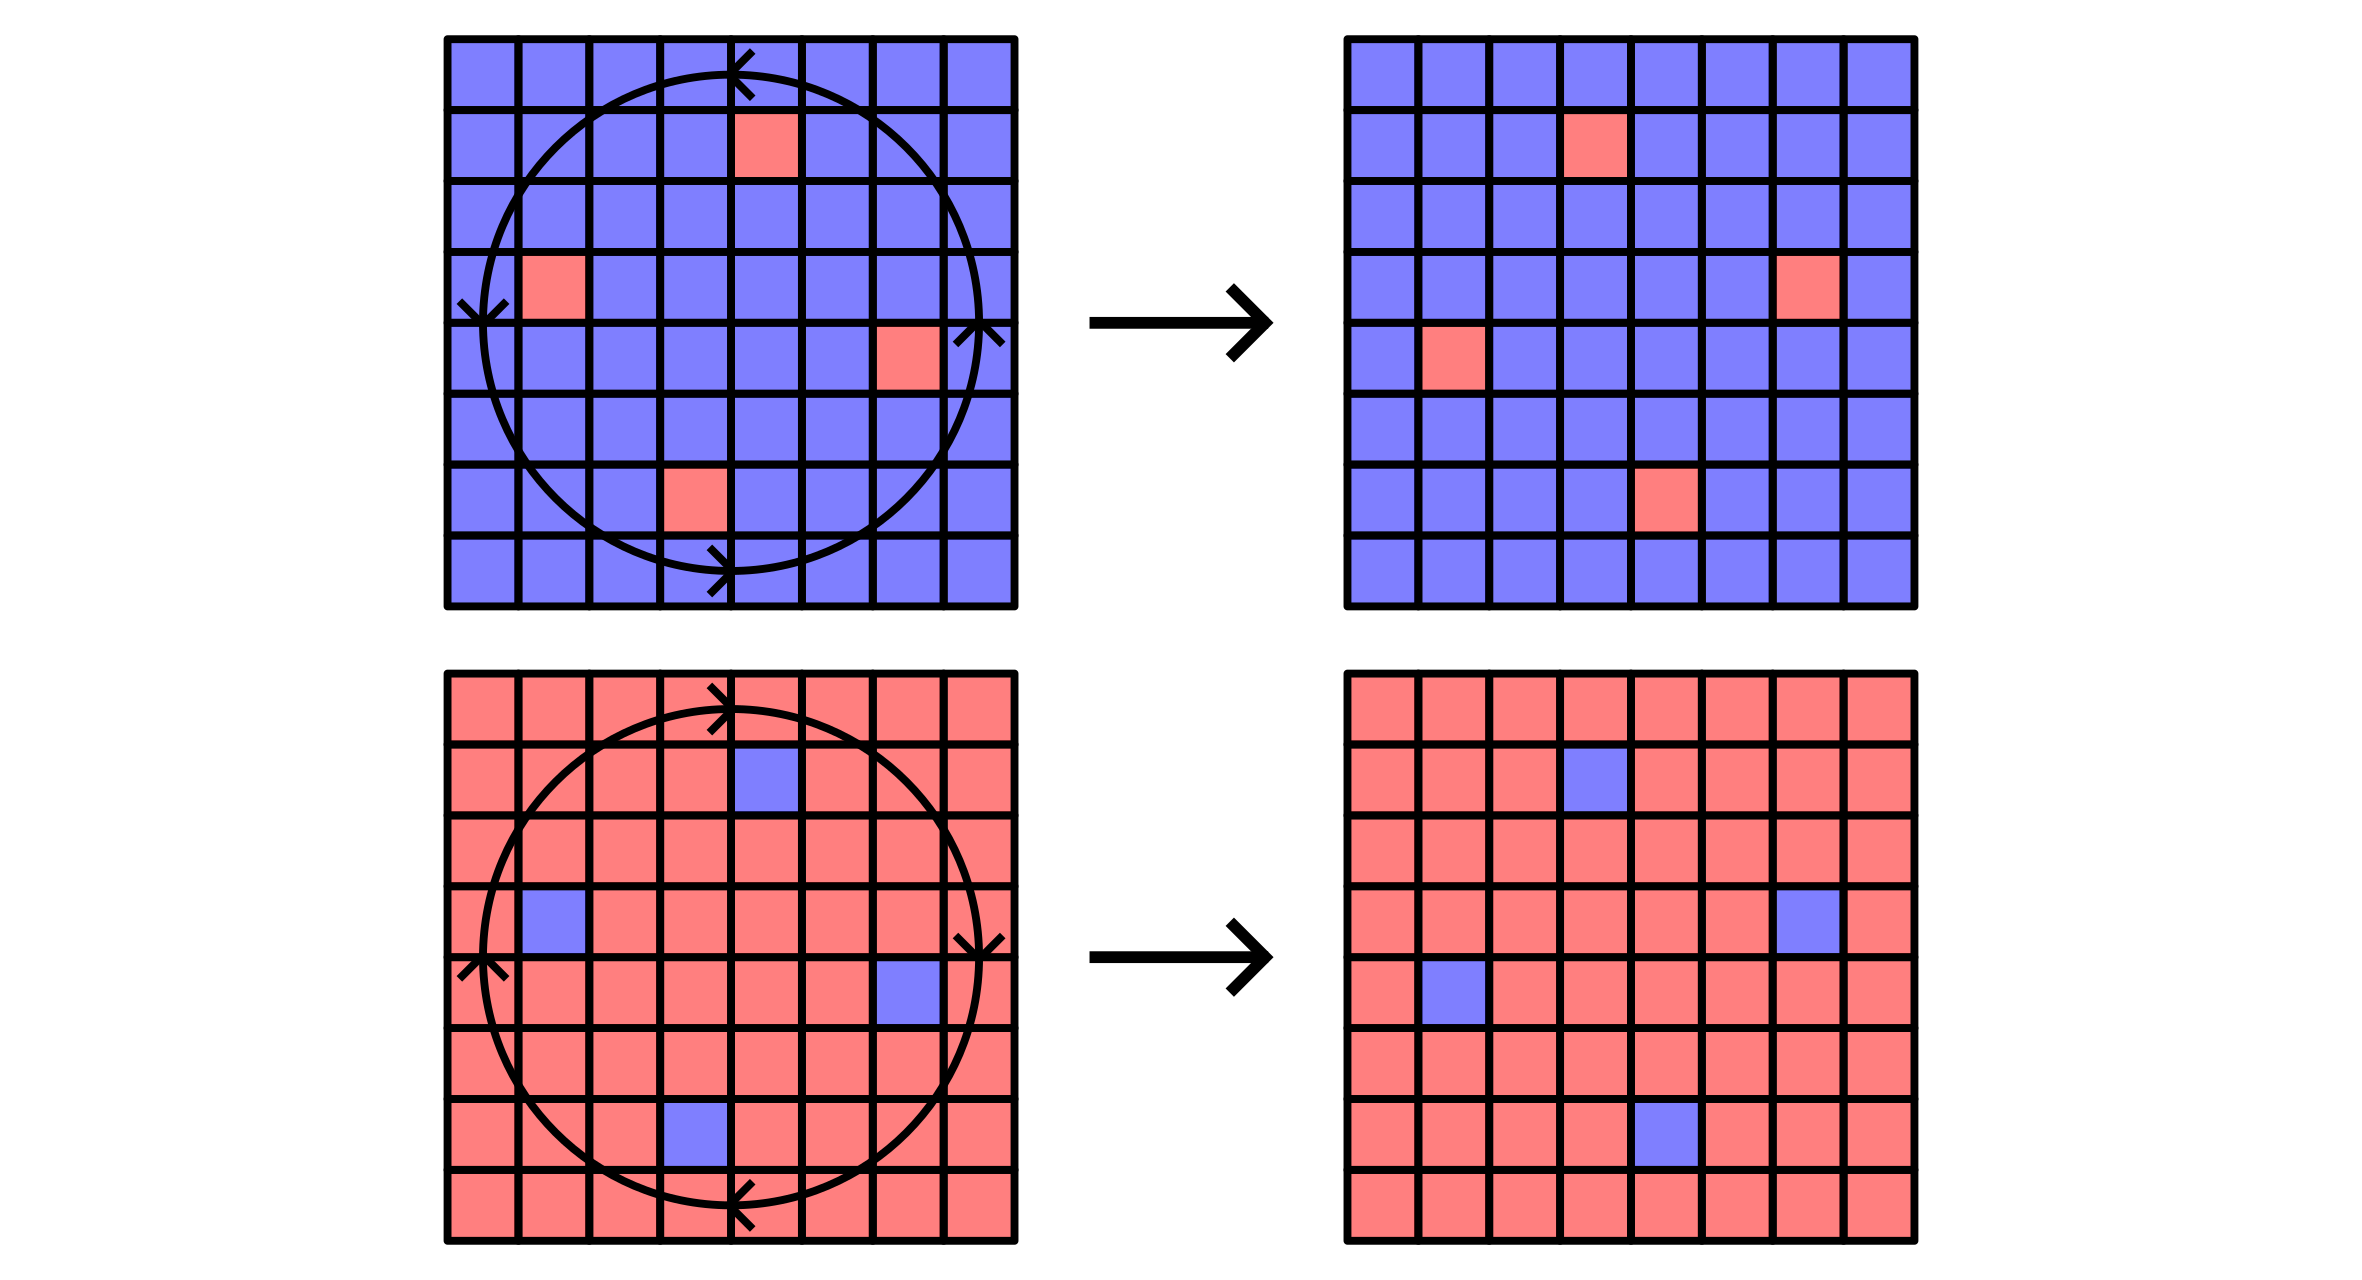
\includegraphics[width=\textwidth]{Figure 7.10.F}
\caption{Rotation ``direction'' depends on interpreting Boolean values as ``electric charge''}
\end{figure}
\noindent
If we use what we learned with the hexagonal example, we can say that $f$ rotated positively and $g$ rotated negatively. In $f$, particles rotating counter-clockwise is positive is the result of antiparticles rotating clockwise. In $g$, antiparticles rotating counter-clockwise is the result of particles rotating clockwise.

Consider our Boolean random walk whose connected cells are shaped like a torus:
\begin{figure}[H]
\centering
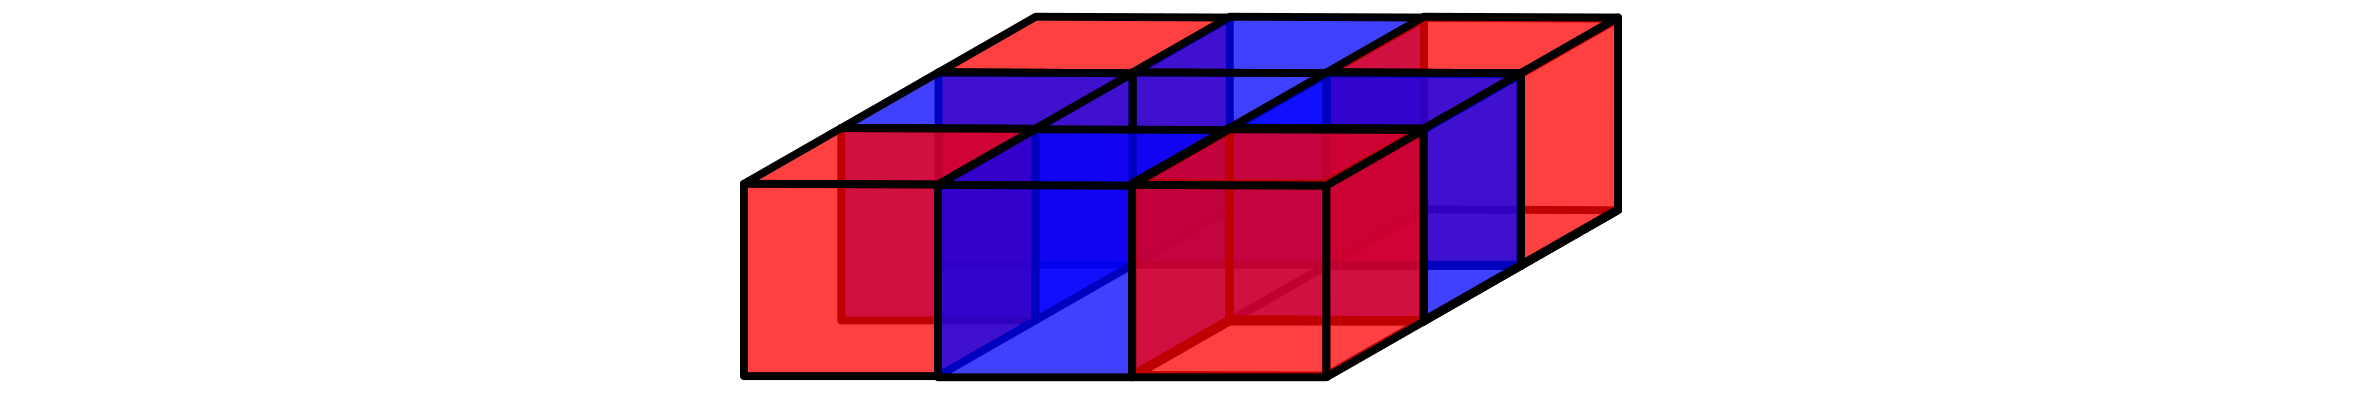
\includegraphics[width=\textwidth]{Figure 7.10.G}
\end{figure}
\noindent
Generalized Stokes theorem says that for an orientable surface that for a differential form $\omega$ and a manifold $\Omega$ that:
$$\int\limits_{\Omega} d \omega = \int\limits_{d \Omega} \omega$$
\noindent in which $d$ is the exterior derivative. The standard definition of curl is a type of differential $2$-form. Since generalized Stokes theorem is intended for orientable surfaces like a torus, we may wish to be careful about integrating the pseudo-curl along a non-orientable surface like a M\"{o}bius strip.

The following image describes how the integral of the curl or pseudo-curl of a function within volume equals the curl along the exterior boundary:
\begin{figure}[H]
\centering
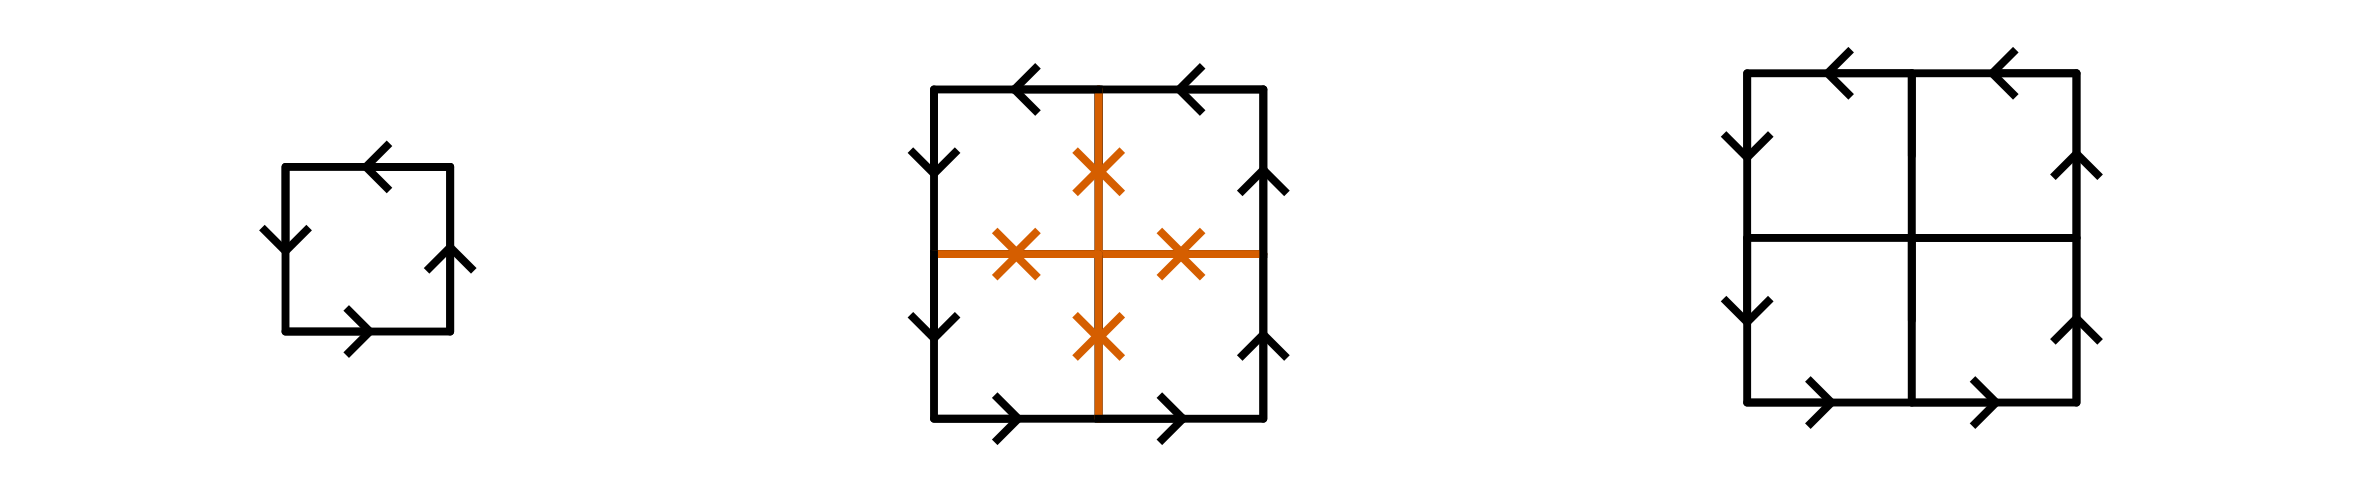
\includegraphics[width=\textwidth]{Figure 7.10.H}
\caption{Measures of curl on the interior portion of cells negate, leaving only the boundary}
\end{figure} \noindent 
The curl of each of these individual paths around each of these four squares should negate should negate along the interior but not about the exterior. Generally, the curl of the interior of a volume $V$ should annihilate itself, leaving the curl along the exterior of $V$.

The main difference between pseudo-curl and the standard definition of curl is that pseudo-curl has more depth of contribution from the outermost cells:
\begin{figure}[H]
\centering
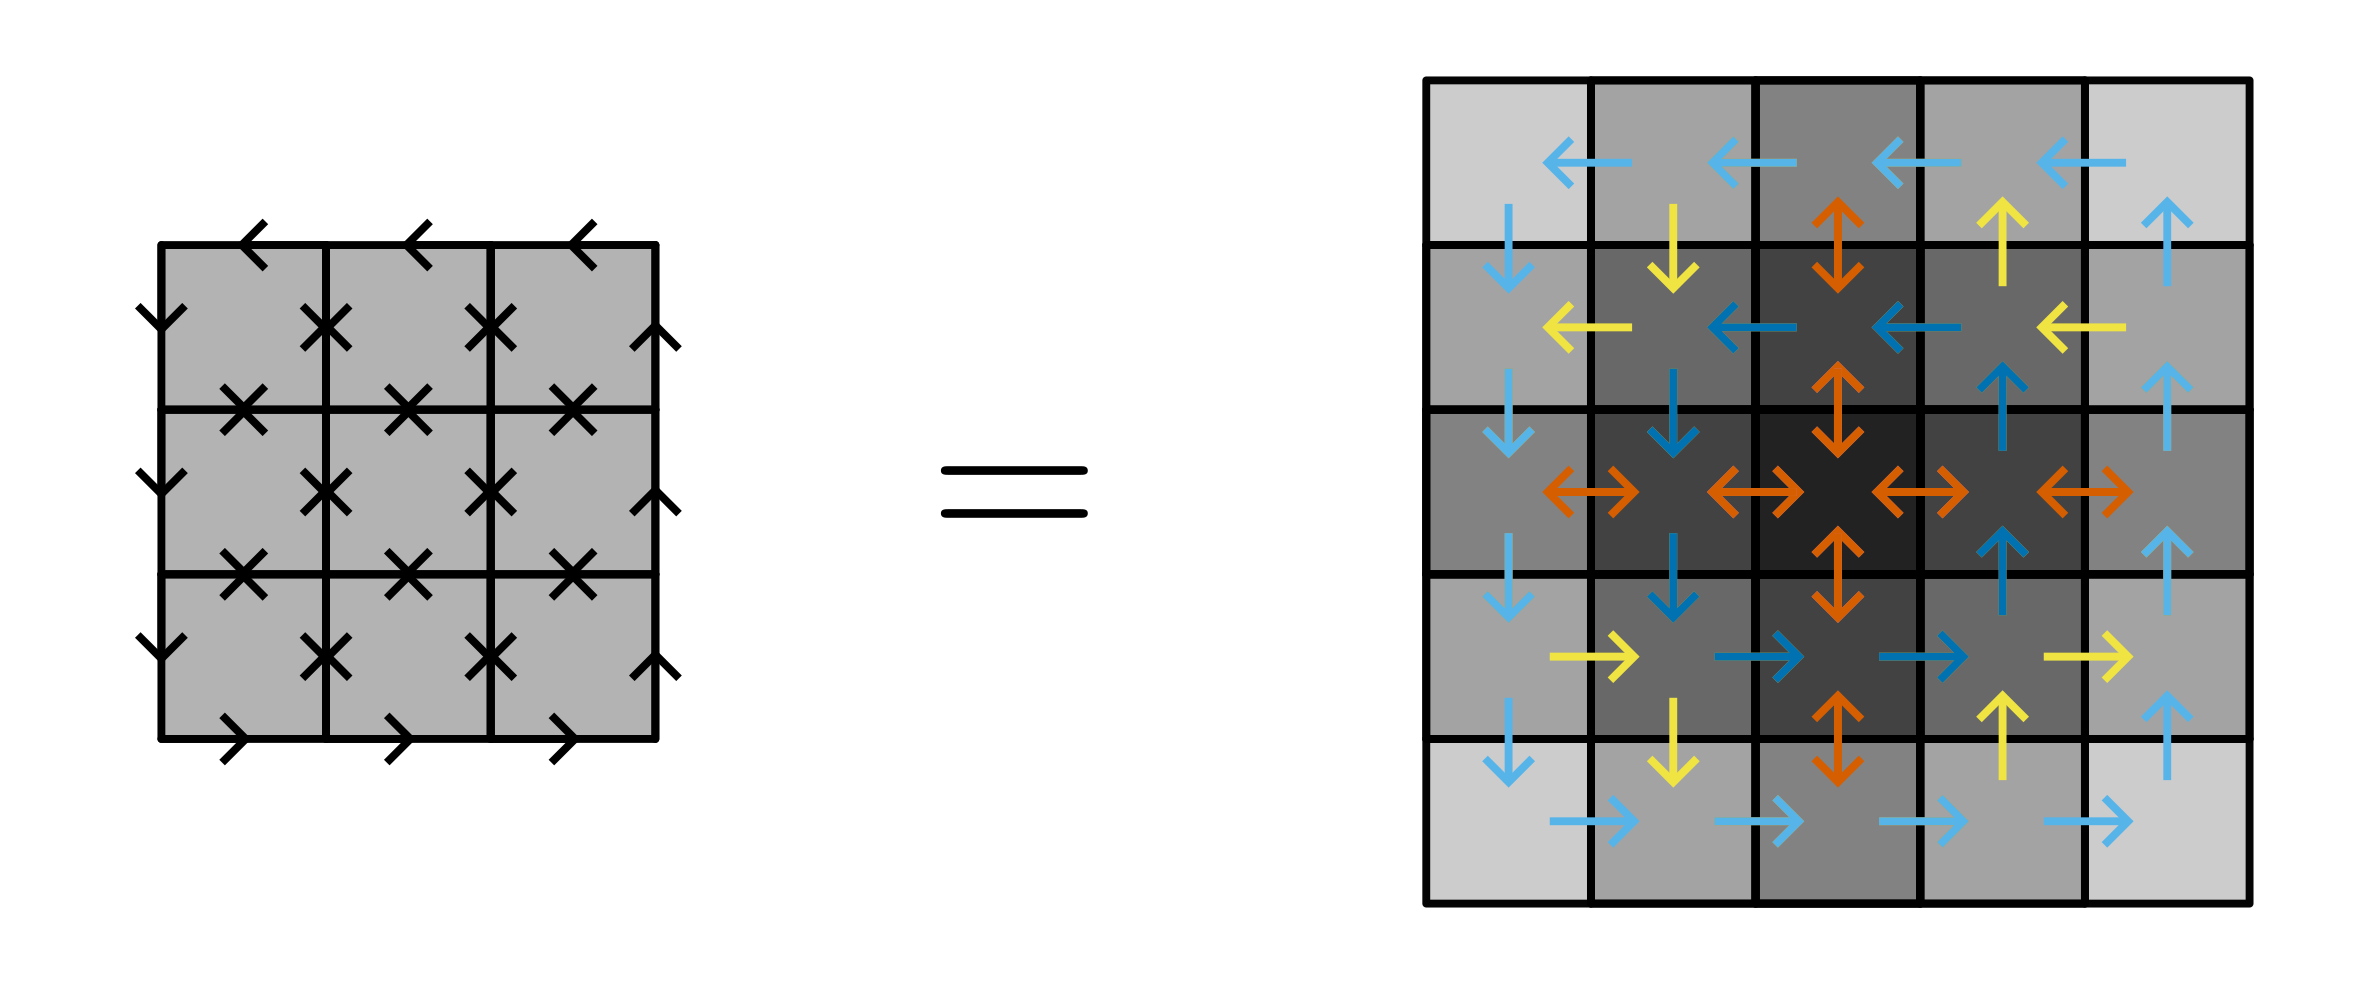
\includegraphics[width=\textwidth]{Figure 7.10.I}
\caption{Measures of pseudo-curl only negate after sufficient depth, due to depending upon neighbors. The innermost dark orange arrows negate, the inner ocean blue arrows measure interior flow, and middle yellow arrows measure exterior flow, and the sky blue outer arrows measure the flow across along neighboring cells.}
\end{figure}
\noindent
Since pseudo-curl depends on the perpendicular flow of adjacent cells, the overall value is sensitive to the depth of consecutive cells in a checker chain. A component graph of the finite-difference graph $T$ is directly related to the idea of a checker chain. 

If the pseudo-curl being measured is an entire graph component (an irreducible checker chain), then the Hamiltonian contribution outside of the checker chain is \textit{almost} zero. For a heavily isolated component, the pseudo-curl is only the interior flow and the exterior flow is zero. For two adjacent components of opposing pseudo-curl, the exterior flow between them is strong.


\chapter{Differential Equations}

\section{Motivations for Learning Differential Equations}
A \textbf{differential equation}\index{differential equation} is an equation that relates the value functions and their derivatives. This vague and general relationship means that many real-life objects or processes can be described with this relationship, such as the motion of fluids and solids. We may wish to describe the density of these materials at any point in time, but an analytic solution may not exist. Therefore, approximating solutions via differential equations are important in fields of applied mathematics. The natural sciences are dedicated to the study of how the natural world changes over time via cause and effect. Accurate approximations allow us to predict the motion of the natural world as well as artificial mechanisms.

\textbf{Diffusion equations}\index{diffusion equation} are used to represent the dispersion of particles in ``empty space'' or heat in material with high thermal conductivity. Boolean random walks is the result of a discrete stochastic differential equation, and it mirrors a Wiener process's continuous stochastic differential equation. Since Boolean random walks may execute any computable function if arranged properly, larger computational structures may encode the rules of any other differential equation.

Allow us a brief aside into the philosophy of objects. Regions of space that are permissible mediums, that tend to spread out and accept information, are called \textit{accepts}. Regions of space that are non-permissible and dense, that tend to join together and reject information, are called \textit{objects}. An object such as an apple objects to information packets of sight, sound, or touch passing straight through them without \textit{interaction}. In the eyes of a cellular automaton, there is no perceptual difference between empty space and colliding objects.

The Schr\"{o}dinger equation is a type of differential that describes the time-evolution of the position wavefunction $\psi(x)$ and the momentum wavefunction $\phi(p)$. Two electron particles in a box must evolve properly while tending to repel each other. Analytic solutions to differential equations with repulsion are tricky because particles cannot be inside of each other. If we move the differential equation into the state space, we can reproduce all dynamics without issue. For any tough equation, the state space dynamics is often simpler than the original equation.

\section{Ordinary Differential Equations}
An \textbf{ordinary differential equation}\index{ordinary differential equation} is an equation that relates the value of a function $f$ to the value of its derivatives $f', f", f^{(3)}$, etc. Specifically, an ODE does this with respect to a single variable such as $x$ or $t$. The simplest ODE is:
$$f(x) = c \cdot f'(x)$$
in which the solution is the exponential function, $f(x) = e^{cx}$. For example, if we have the form $f(x) = -1 f'(x)$, then our solution to the equation is $f(x) = e^{-x}$:
\begin{figure}[H]
\centering
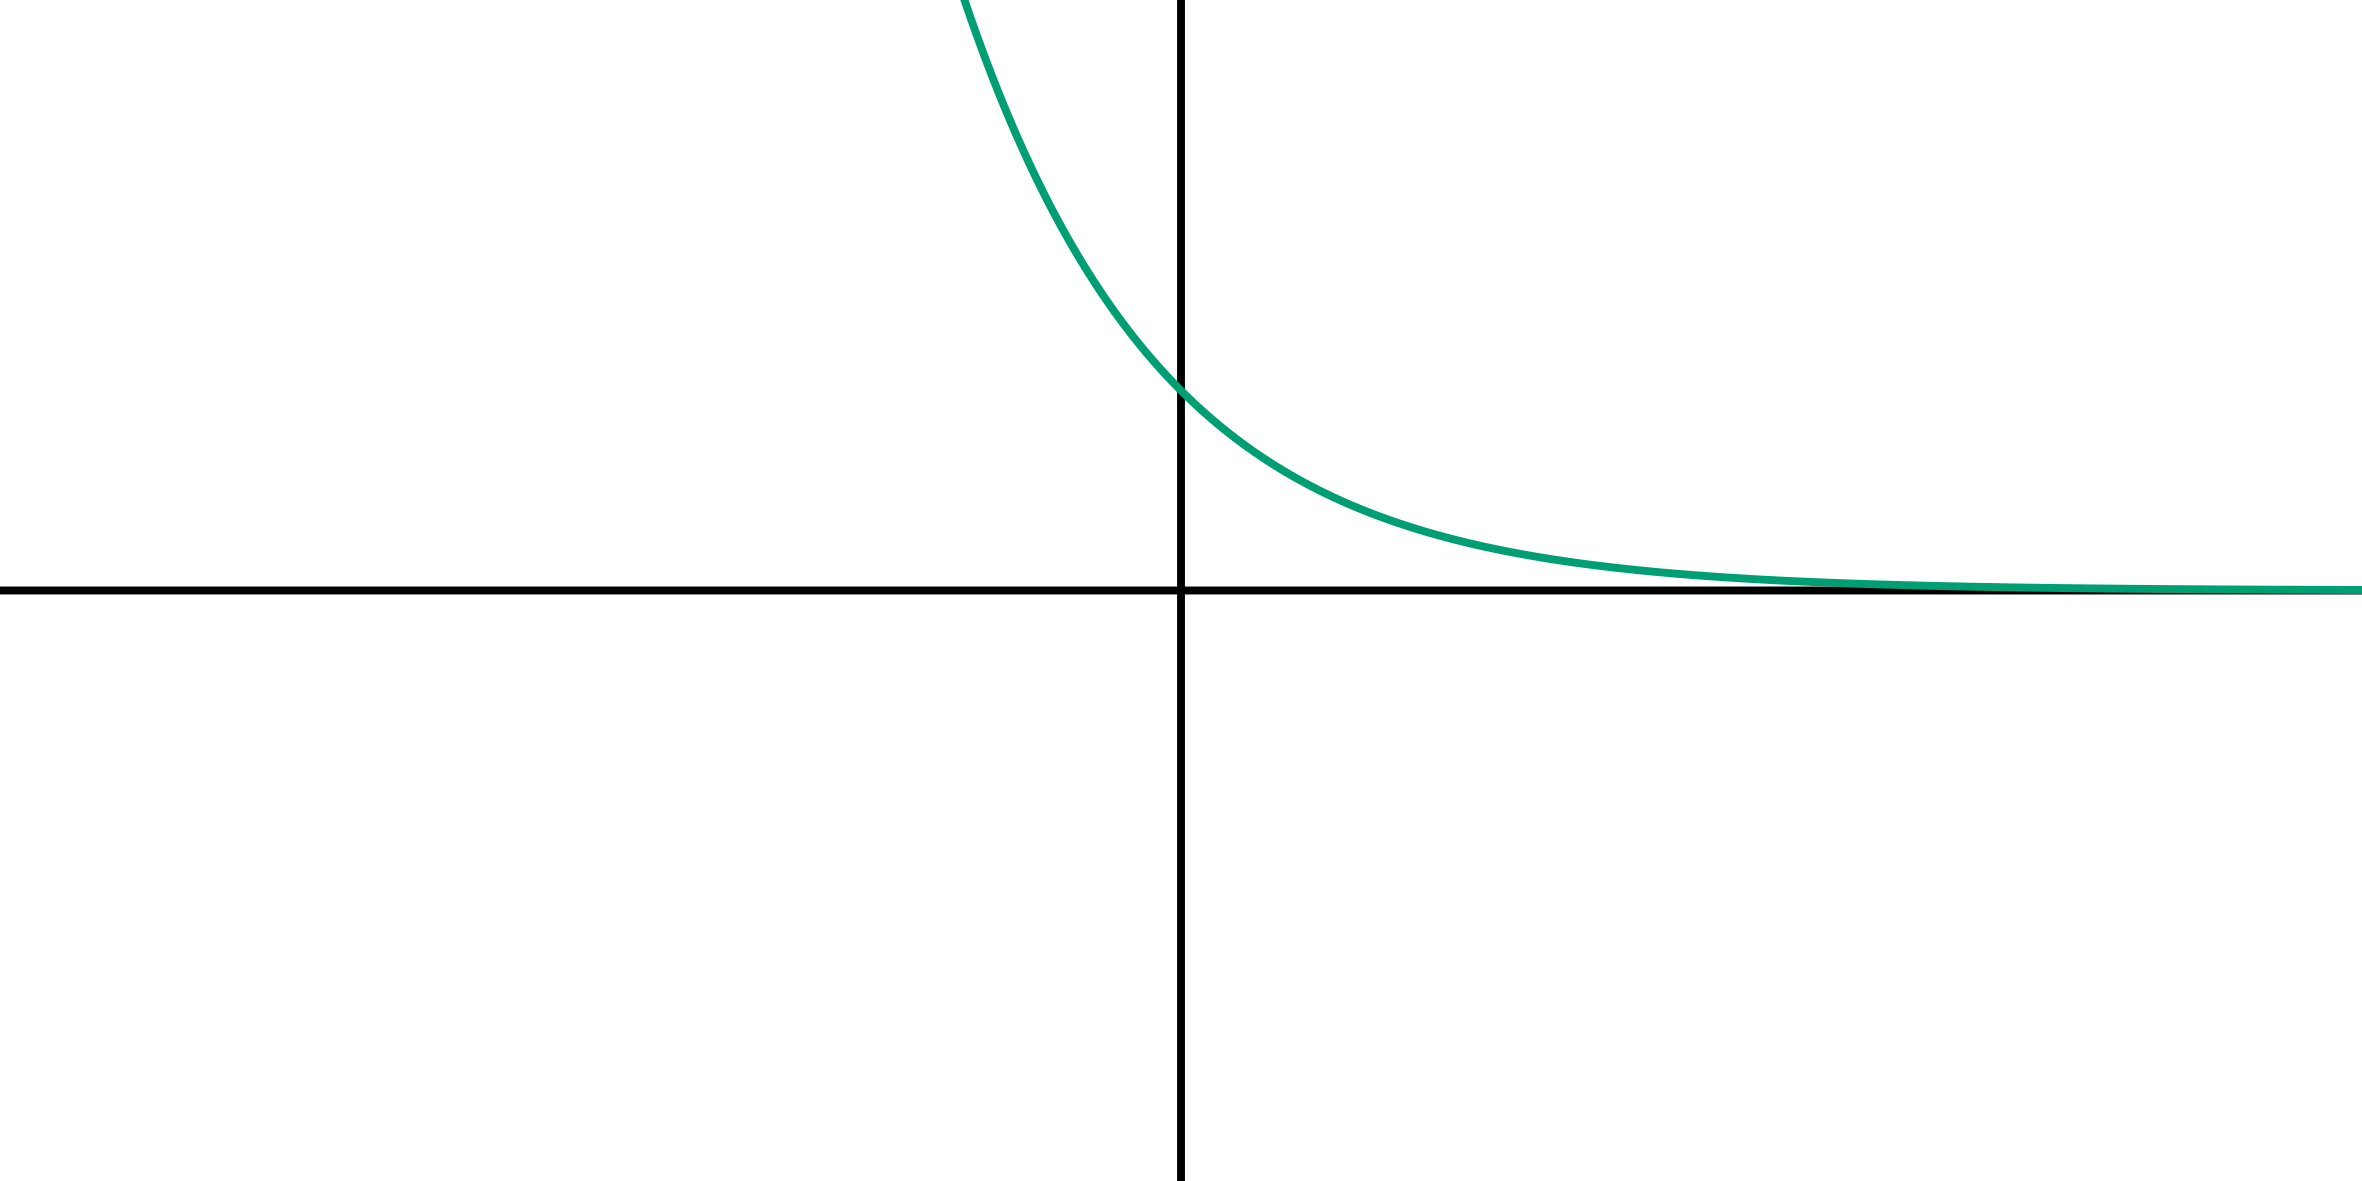
\includegraphics[width=\textwidth]{Figure 8.2.A}
\caption{A first-order ODE with $c=-1$}
\end{figure}
\noindent
Since this ODE expresses a relationship in which the highest derivative is the first derivative, this is called a first-order ODE.

In differential equations, we are usually working with the equations of the form:
$$f(x) = \sum\limits_{n=1}^\infty a_n \frac{d}{dx}f(x),\quad \sum\limits_{n=1}^\infty a_n < \infty$$
However, we often do not know the function $f$ that makes the equation true. The function $f$ does not have an analytic or closed-form expression in many cases, analytic in the sense that the function has a convergent Taylor series:
$$f(x) = \sum\limits_{n=1}^\infty a_n (x-\mu)^i, \quad a_n = \frac{f^{(n)}(\mu)}{n!}$$
about the point $\mu$. The exponential function has the unique property of being its own scaled derivative as well as sine and cosine having a similar relation due to Euler's formula:
$$e^{ix} = \cos(x) + i \sin(x)$$
This means that we can often run numerical simulations of the differential equation in question.

\textbf{Linear ordinary differential equations}\index{linear ordinary differential equations} are ordinary differential equations of the form:
$$\sum\limits_{n=1}^k a_n f^{(n)}(x) = g(x)$$
in which $a_1,...,a_k$ are scalar constants. A linear ODE equation with the added constraint of $g(x)=0$ is called a \textbf{homogeneous linear ordinary differential equation}\index{homogeneous linear ordinary differential equation}. Homogeneous LODEs are special in that they can be solved exactly since $f(x) = e^{cx}$ in all cases such that:
$$ a_0 f(x) + a_1 f'(x) + a_2 f"(x) +... = 0$$
$$\iff a_0 f(x) + a_1 c f(x) + a_2 c^2 f(x) +... = 0$$
$$\iff a_0 + a_1 c + a_2 c^2 + ... = 0$$
is a called a characteristic polynomial equation in which $c$ is the root.


\section{Partial Differential Equations}
A \textbf{partial differential equation}\index{partial differential equation} is an equation that relates the value of a multivariable function $f(\boldsymbol x)$ to the value of its partial derivatives $\frac{\partial}{\partial x_i}f(\boldsymbol x)$. We are most interested in relating changes in the value of a function $f$ in time with its neighboring points in space:
$$\frac{\partial}{\partial t}f = \frac{\partial^2}{\partial x^2}f$$
This equation is deceptively simple as many functions may fulfill this equation exactly. A prime example is diffusion of a gas particle in $1$ dimension:
\begin{figure}[H]
\centering
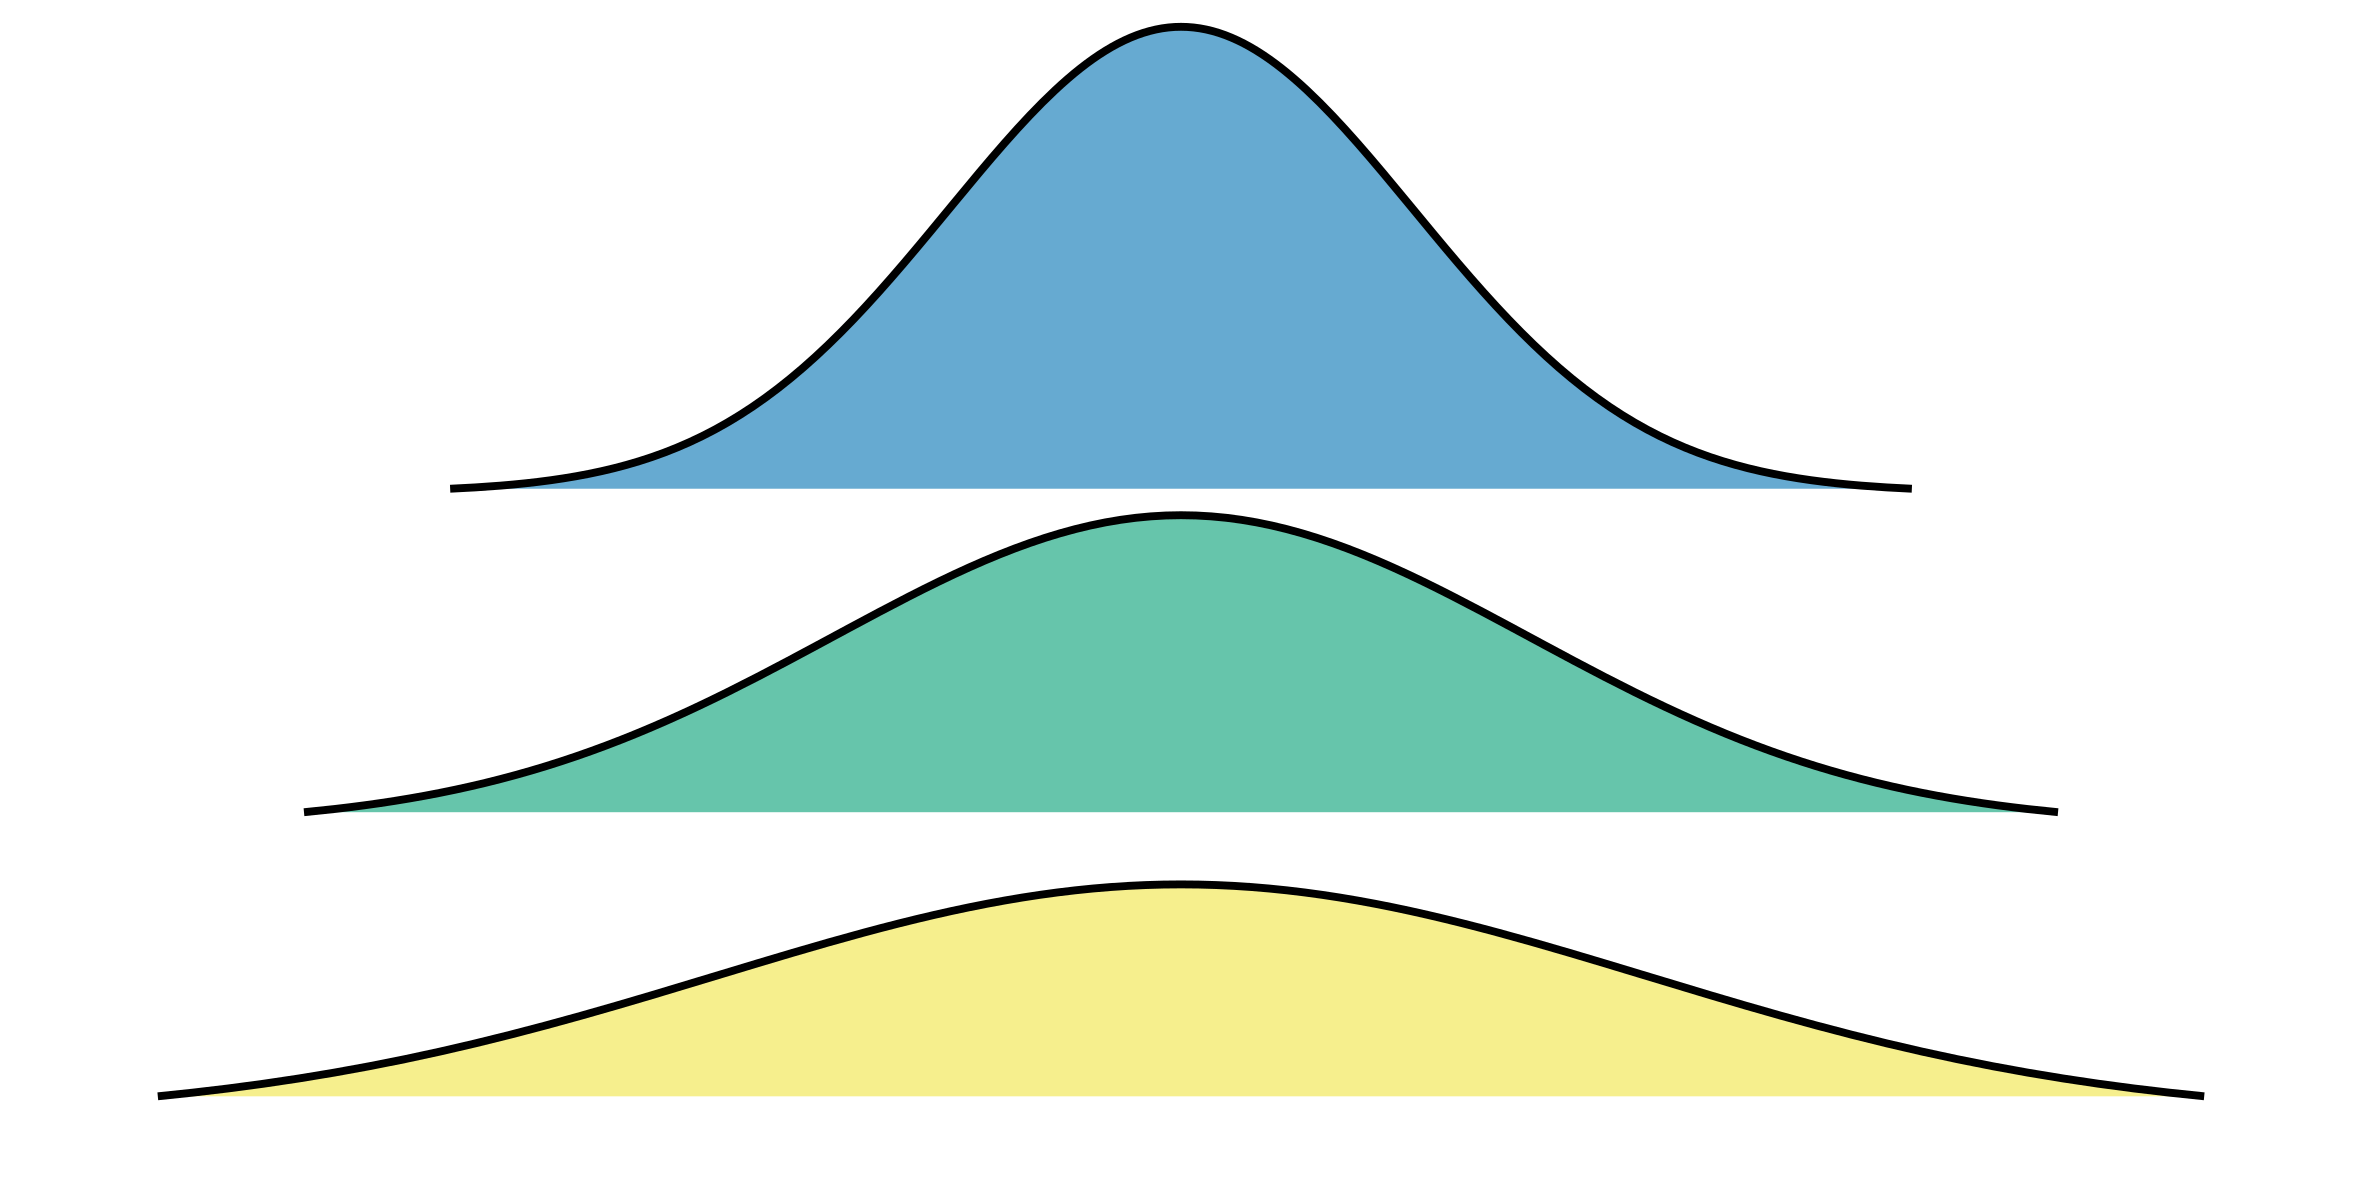
\includegraphics[width=\textwidth]{Figure 8.3.A}
\caption{The diffusion of a gas in 1D space at various time steps}
\end{figure}
\noindent
The diffusion of such as particle obeys a $\textnormal{Normal}(0, \sqrt{t})$ distribution. Every one of these distributions is a solution, forming a family. The \textit{domain} of $f$ will additionally influence the family of solutions. If we instead restrict the domain to a box, the particle will diffuse like the above example until it hits the walls.

The majority of physical phenomena relevant to human interest obey the evolution of some kind of PDE. This is because the spatial function that represents the phenomenon must relates to itself in time.\footnote{Most natural sciences describe permutations of space in time. In fact, most human labor is permutations of space in time.} Thermodynamics, electrodynamics, fluid dynamics, and more are modeled via continuous evolution of space across time while conserving some measure of energy, such as energy or mass. The continuous deformation of this field is approximated by:
$$f(x, t+ \varepsilon) \approx f(x, t) + \nabla_x f(x,t) \cdot \partial \boldsymbol x$$
$$\iff \nabla_x f(x,t) \cdot \partial \boldsymbol x = f(x, t+ \varepsilon) - f(x, t)$$
Note how this first-order Taylor expansion is some kind of non-linear differential equation. In physics, this is a discrete approximation of how some physical system works. In Boolean mechanics, this relation is almost exactly true due to being of discrete value, time, and space.

Stochastic partial differential equations generalize PDEs with a random-valued function in the equation, often denoted as $\varepsilon (\boldsymbol x,t)$. Such a \textit{noise function} $\varepsilon$ can be independent of time as $\varepsilon(\boldsymbol x)$ or even independent of adjacency or spatial correlations as $\varepsilon( t)$. Stochastic PDEs are useful when modeling phenomena that are random. It is also useful in describing systems in which information loss means precision in representation is less important. As an example, computer graphics is less concerned with exact physics than fast algorithms that approximate reality for fluids, smoke, or terrain of a world. In engineering or physics, reliability under random circumstances is critical.

The diffusion of heat and fluids are very similar. Fluid particles tend to flow to empty regions to fill them, similarly to how heat tends to flow from hotter regions to colder. However, this is only a statistical tendency rather than a guarantee. Temperature is itself a macroscopic phenomenon; energy may sometimes transfer unevenly at the microscopic level. Boolean random walks is an excellent study of how particles tend to spread out yet are not forbidden from doing so.

\section{Diffusion and Heat Equation}
The \textbf{diffusion equation}\index{diffusion equation} is a second-order partial differential equation in which the density function $f$ at position $x$ and time $t$ diffuses in space over time according to the relationship:
$$\frac{\partial}{\partial t} f(x,t) = \nabla \cdot (D(x,t) \nabla f(x,t))$$
in which $\nabla \cdot$ is the divergence operator, $\nabla$ is the gradient operator, and $D$ is the diffusion coefficient for each spacetime coordinate $(x,t)$. If $D$ is constant across time and space, then the diffusion equation reduces to the heat equation:
$$\frac{\partial}{\partial t} f(x,t) = D(\nabla \cdot\nabla f(x,t)) = D \sum\limits_{i=1}^d \nabla^2_{ii} f(x,t)$$
in which $\nabla^2$ is the \textbf{Hessian operator}\index{Hessian operator} that produces the second-order partial derivatives of a function, $d$ is the dimensionality of space, and $\nabla \cdot \nabla$ is the \textbf{Laplace operator}\index{Laplace operator}. The Laplace operator is the sum of the diagonals of the Hessian operator.

For sufficiently dense Boolean random walks, the diffusion coefficient $D$ is not constant due to possible lockouts when selecting a maximal independent set, as defined in \textit{\S 7.7 n-Flip Chordings and Orderings}.
\begin{figure}[H]
\centering
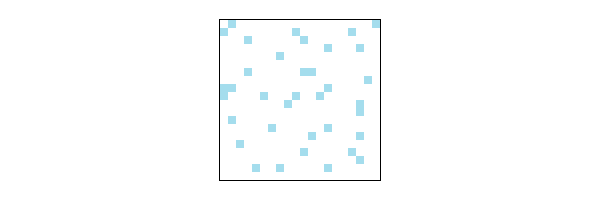
\includegraphics[width=\textwidth]{Figure 8.4.A}
\caption{A somewhat dense Boolean random walk}
\end{figure}
\noindent
If too many particles bunch up in a checker chain, a smaller proportion of maximal independent sets are a \textit{maximum} independent set. It is common to have less than $\min(k, N-k)$ pairs occurring when the density is too high.

For sparse Boolean random walks, the random walkers are far apart that we may assume approximate statistical independence. 
\begin{figure}[H]
\centering
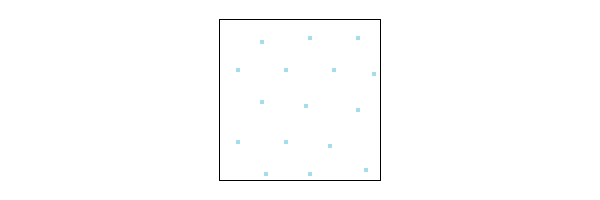
\includegraphics[width=\textwidth]{Figure 8.4.B}
\caption{A sparse Boolean random walk}
\end{figure}
\noindent
That essentially means that each particle of the Boolean minority class is almost always moving due to most maximal independent sets being maximum independent sets. It is uncommon to have less than $\min(k, N-k)$ pairs occurring at any given time. 

Our representation of the Boolean random walk must be able to account for directional imbalances for each face of a cell. Recall the heat equation:
$$\frac{\partial}{\partial t} f(x,t) = D \sum\limits_{i=1}^d \nabla^2_{ii} f(x,t) $$
In our discrete version of the diffusion equation, we may cheat the treatment of an analytic formulation by separating derivatives into directional derivatives such as $x_{-d}, x_{-d+1},...,x_0,...,x_{d-1}, x_d$. The oriented forward difference operator $\Delta_{x_{k}}$ has a backwards difference operator that is $\Delta_{x_{-k}}$ such that:
$$\Delta_t f(x,t) = \sum\limits_{i=-d}^d \chi_i \Delta_{x_{i}} f(x,t)$$
is the Boolean heat equation in which $\chi_i (x,t)$ gives a valid random chording of $\Delta_t f(x,t)$, or rather $\Delta X_t$ if we prefer Markov chain notation. The \textbf{chording function}\index{chording function} $\chi_i$ is a probability distribution over non-zero cell differences, as determined by the vertices of the finite-difference graph $T$ for a maximal independent set $H$.

This Boolean diffusion equation separates the forward difference and backward difference into separate parts, a sort of pseudo-Laplace operator. The chording function $\chi_i$ carries information about which cells may pair in a bit flip. We might interpret that a chording function is like a constant diffusion coefficient $D$ once chosen. The symmetry of a chording function is described like so:
$$\chi_i f(x, t) = \chi_{-i} f(x + v_i,t)$$
in which $v_i$ is a unit vector in the direction $i$. It basically means that a cell's forward chording corresponds to the backward chording with the cell in front of it, and a cell's backwards chordings correspond to forward chordings with the cell behind it.

Observe the following example 2D system with a fixed chording:
\begin{figure}[H]
\centering
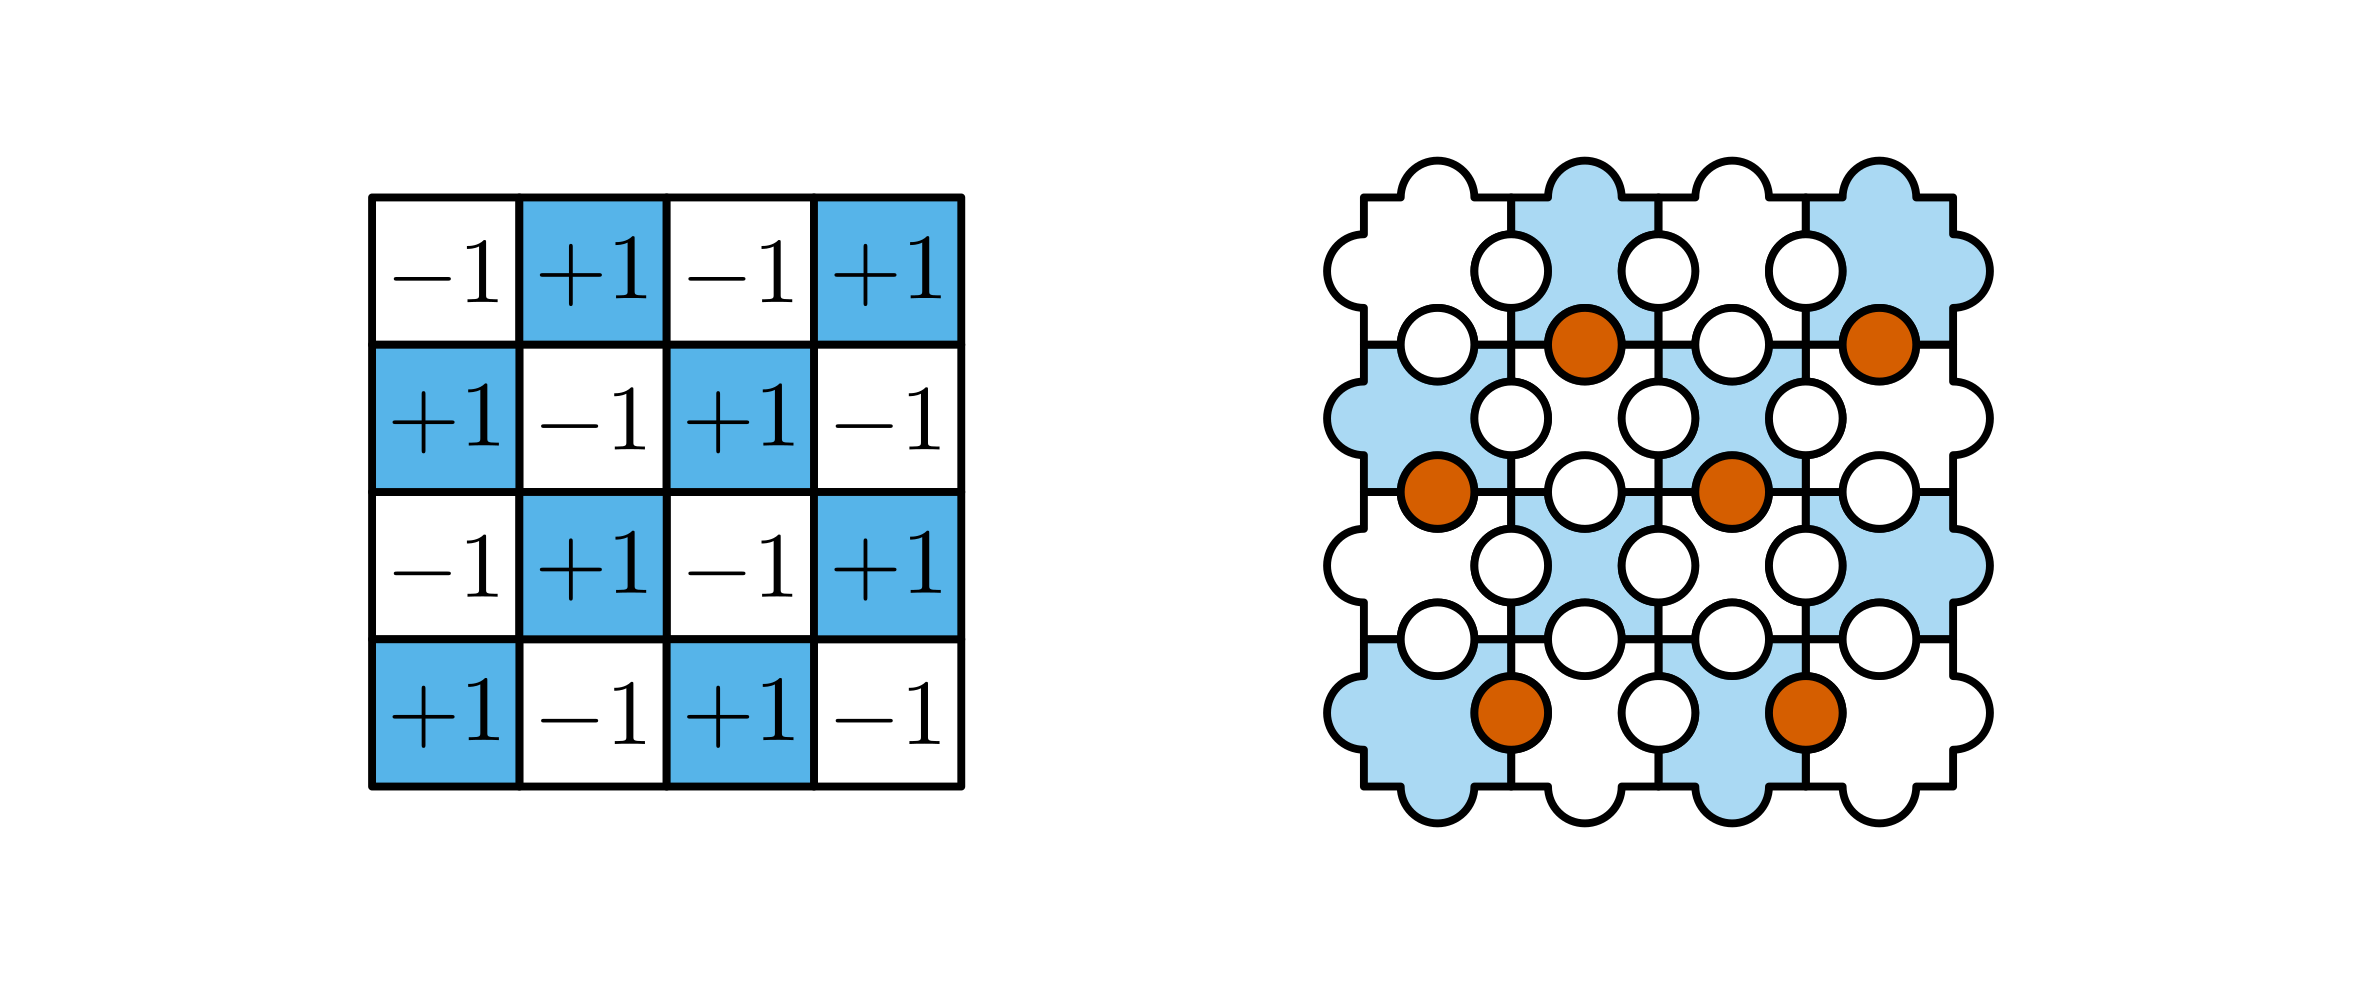
\includegraphics[width=\textwidth]{Figure 8.4.C}
\caption{A maximal independent set of vertices that leaves some Boolean hyperedges untouched}
\end{figure} \noindent
Due to the definition of the restrictions we have defined, we have exactly:
$$X_{t+1} = X_t + \Delta X_t$$
or equivalently in diffusion equation notation:
$$f(x,t+1) = f(x,t) + \Delta_t f(x,t)$$
A cell with a value of $+1$ making a switch with a $-1$ cell has a difference of $-2$. In this case, $f(x,t)=+1$, $\Delta f(x,t) = -2$, and the new value is thus $f(x, t+1) = +1-2=-1$.


In time series analysis, the forward difference operator $\Delta$ and backshift operator $B$ are defined as:
$$\Delta_t X_t = X_{t+1} - X_t$$
$$B_t X_t = X_{t-1}$$
and $B \Delta$ likewise is the backward difference operator. We may also infer that:
$$\Delta_t X_t = B_t^{-1} X_t - X_t = (B_t^{-1}-1) X_t$$
$$\Delta_t = B_t^{-1} -1 \iff B_t^{-1} = 1+ \Delta_t$$
Notice the similarity to our relevant Boolean diffusion equation:
$$f(x,t+1) = B^{-1} f(x,t) = f(x,t) + \delta_t f(x,t)$$
The definition of the shift operator $e^{\frac{\partial}{\partial t}} = B^{-1}$ is usually more convenient, and we prefer the notation of the special case of working with some matrix with eigenvalue matrix $\Lambda = \lambda I$.


\section{Normal Modes and Harmonic Functions}
A \textbf{normal mode}\index{normal mode} is a special function $f$ upon a domain $X$ that oscillates, and the value of $f$ only changes according to multiplication by an eigenvalue $\lambda$ such that:
$$f(x, t) = f(x, 0) \lambda^t$$
in which is a complex eigenvalue $\lambda \in \mathbb C$. Normal modes are of critical importance because they reduce the modeling of complicated objects to linear differential equations.

The normal modes of simple objects such as a string can be used to model both the fluctuations of a stringed instruments and the heat equation for a linear object:
\begin{figure}[H]
\centering
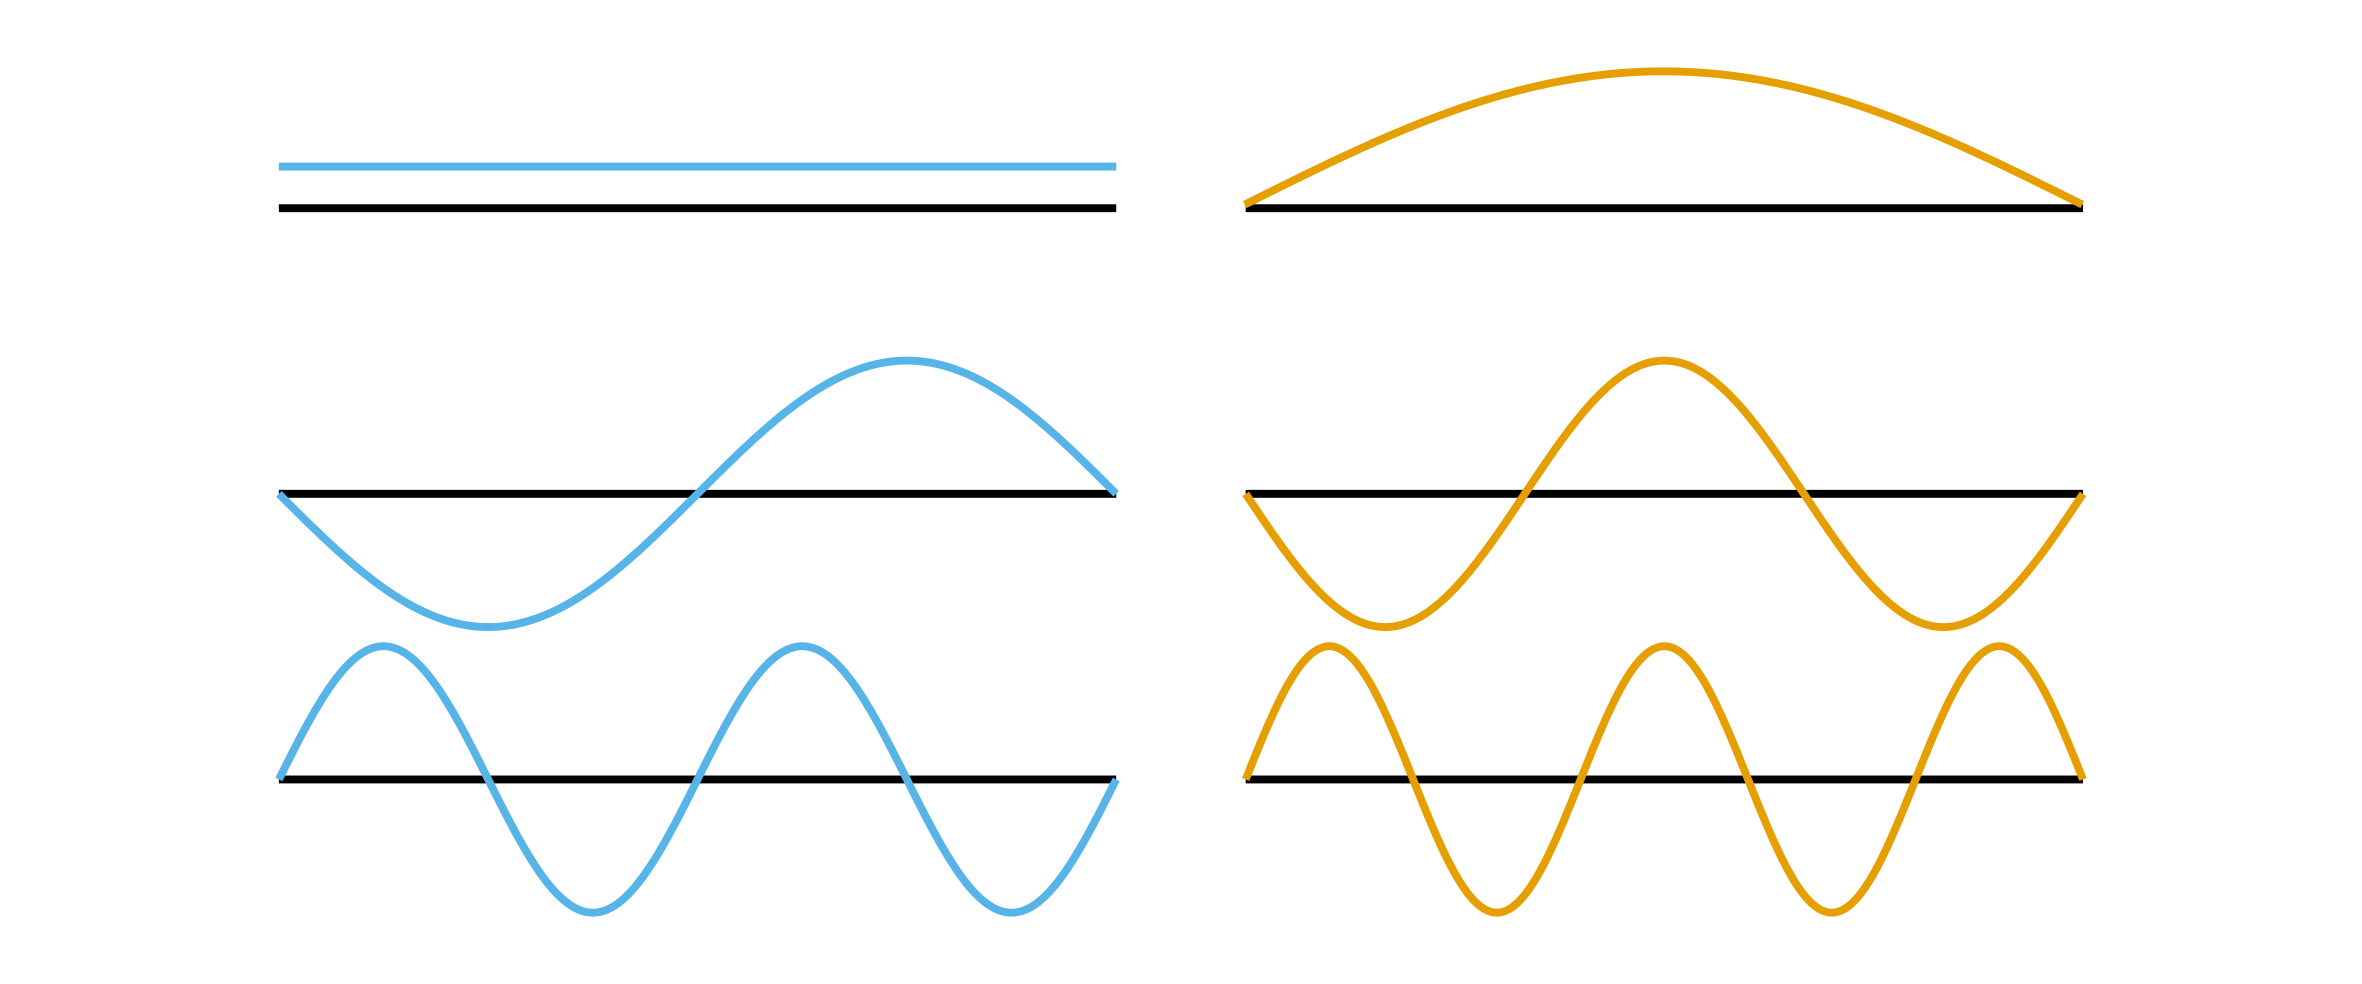
\includegraphics[width=\textwidth]{Figure 8.5.A}
\caption{Normal modes of a string}
\end{figure} \noindent
The higher frequency modes decay faster than the low frequency modes. The Fourier transform is exactly the normal modes of the displacement of a vibrating string from its center as well as the temperature of a pole. Normal modes for a string linear object are relatively simple since they are merely higher frequencies waves. Unusual shapes such as an acoustic guitar body have more complex normal modes.

Suppose that I have the normal modes of a domain $X$ with shapes
$$f_1(x), f_2(x),..., f_n(x)$$
The key property of a sequence of normal modes is that they are orthogonal, $f_i \perp f_j$ for $i \neq j$. If I have $n$ eigenvalues $\lambda_1, \lambda_2,...,\lambda_n$, then I can obtain the time evolution of a shape upon $X$ as the function:
$$f(x, t) = \sum\limits_{i=1}^n a_i f_i(x) \lambda_i^t$$
in which $a_i$ is the initial magnitude of the normal mode. With a sufficiently large amount of normal modes and eigenvalues, we can model almost any function on the domain $X$. Similarly, a Fourier transform forms an infinite sequence of linearly independent functions with which to describe any arbitrary function. 

These normal modes are excellent tools for understanding systems that we know to be bounded, such as the surface of a drum, but they struggle for systems that behave randomly or chaotically. The issue is not that normal modes upon measurable objects themselves are useless, but incomplete. We need to understand normal modes of the state space $\mathcal X$.

The normal modes of a stochastic process give a more complete picture of how random objects behave and how to efficiently control random processes. The goal of any machine is to act as a \textit{state space controller}. In terms of Boolean random walks, a machine acts as a state space controller. That means interfering with the normal modes of a smaller system. However, it is unlikely to be able to turn any complicated even state at an even time step into its Boolean inverse odd state at an even time step (e.g. an electron into a positron) by breaking the $2$-cyclic rule of random walks.


\part{Boolean Mechanics Principles}

\chapter{Boolean Mechanical Systems}
\section{Motivations for Boolean Mechanical Systems}
\textbf{Boolean mechanical systems}\index{Boolean mechanical systems} are not merely a generalization of random walks. They are the culmination of all the ideas discussed thus far. The previous chapters walk through seemingly disconnected fields of mathematics and how each field might provide a unique perspective on Boolean random walks. Together, they provide the basis for a dynamical system that will compute every computable function. A theory of every computable function.

Long sought in physics is the \textbf{theory of everything}\index{theory of everything}, the singular theory that describes all the phenomena in our universe. Such a theory would be able to describe the largest galactic cluster and the smallest particle using the same principles. In that sense, it is meant to describe all noumena. Noumena are objects as they truly are independently of the senses, a singular interpretation. Phenomena are objects are they appear dependent upon the senses, multiple interpretations derived from a noumenon. What do you make of a reality in which sensing or perceiving an object truly changes how it behaves? The answer to this question is unresolved in quantum mechanics but obvious in Boolean mechanics or cellular automata in general. A theory of everything in physics requires uniting the continuous field of gravity in general relativity and the discrete forces of quantum mechanics in a way that predicts all physical phenomena.

A theory of every computable function merely requires consistent notation that unifies different branches of mathematics. Much less ambitious and more broadly applicable, though I doubt it will make headlines or secure grant funding.

\section{Notation and Convention}
Boolean statistical mechanics integrates seemingly unrelated branches of mathematics, each one with a unique genealogy and rich history that resulted in independently developed notations and conventions. A united set of notations is used throughout this textbook to clearly communicate how deeply interwoven these concepts are. Consistency and clarity in notation aids in the learning synthesis process, thus these are the default meanings of the symbols used in each section of a chapter unless specified otherwise.

A Boolean mechanical system $X_t$ is a random variable $X$ at time $t$. It is a lattice of cubic cells that take upon a value from the Boolean set $\mathbb B_\pm = \{-1, +1\}$, and each cell of the lattice is defined by a $d$-dimensional coordinate $x=(x_1,x_2,...,x_d$). Each time step $t$ is an element of the integers $t \in \mathbb Z = \{...,-2,-1,0,1,2,...\}$. A finite size Boolean mechanical system at time $t$ has dimensional lengths $(n_1, n_2,...,n_d)$ for its $d$ dimensions, and the total system size is $N = \prod n_i$.\footnote{A dimensional length of $n_i = 1$ is degenerate, meaning the $i$-th dimension may be omitted. If I have dimension lengths of $(12, 4, 1)$, then it will behave indistinguishably from a two dimensional system of lengths $(12, 4)$.}. An infinite size Boolean mechanical system has one or more of these dimension lengths as infinite in length. Each cell of a $d$-infinite Boolean mechanical system has each coordinate $(x_1,x_2,...,x_d$) as an element of the integer lattice $\mathbb Z^d$. The transition function $f$ for a given system $X_t$ applies Boolean measure to the position coordinate $x$ and time coordinate $t$ such that $f(x,t) \in \mathbb B$ for all $(x,t)$. The probability function $\mu$ applies a measure to the set of possible configurations of $f(x,t) = X_t$ as a $\sigma$-algebra of the state space $\mathcal X$.

A Boolean random walk is a specific \textbf{pushforward operator}\index{pushforward operator} $\Lambda_\sharp$: $\mu_t \rightarrow \mu_{t+1}$ upon the probability measure $\mu$ with $\Lambda$ as its eigenvalues. The pushforward operator creates a system with local behavior that is indistinguishable from a simple random walk. Let $E_s$ be an element of the sigma algebra at time $s$, and we define the pushfoward operator such that:
$$\Lambda_\sharp = \frac{f(x,t+1)}{f(x,t)} = \frac {\mu_{t+1}(E_{t+1})} {\mu_{t}(\Lambda^{-1} E_{t+1})}
= \frac {\mu_{t+1}(\Lambda E_{t})} {\mu_{t}(E_{t})}
$$
Our pushforward operator is the result of placing our eigenvalue set $\Lambda$ between a our eigenbasis $\Phi$ and its inverse $\Phi^{-1}$ like so: 
$$\Lambda_\sharp = \Phi \Lambda \Phi^{-1}$$
This is exactly the stochastic matrix $P$, meaning any specific state distribution for $f(x,t)$ is a row from $P$ corresponding to the initial state $f(x, 0)$. A Boolean random walk is our default assumption for a Boolean mechanical system due behaving like a fluid.

A finite system $X_t$ is said to be in its critical state if $k = N-k$, or the number of particles equals the number of antiparticles. Particles are assigned a Boolean value of $+1$ and antiparticles are assigned a Boolean value of $-1$. We alternatively call this a \textit{dense} system. A finite system $X_t$ is said to be \textit{sparse} if $k << (N-k)$ or $k >> (N-k)$, or one class dramatically outnumbers the other.
\begin{figure}[H]
\centering
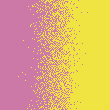
\includegraphics[width=6cm]{Figure 9.2.A}
\caption{This system is dense near the center and sparse near the edges}
\end{figure} \noindent
In this example, particle and antiparticles are dense near the center.\footnote{This is the cover image.} As the system becomes sparse, the number of permutations for a maximal independent set becomes less varied.

The transition function $f$ is a probability kernel, defining a probability distribution for traversed path from the initial state $f(x, 0)$ to the future state $f(x,t)$. A different probability distribution is defined contingent on the time value $t$ and the initial state $f(x, 0)$. It is helpful to think of it that way because it may be defined recursively using our Boolean diffusion equation:
$$\Delta_t f(x,t) = \sum\limits_{i=-d}^d \chi_i \Delta_{x_{i}} f(x,t)$$
$$f(x,t+1) = f(x,t) + \Delta_t f(x,t) = (1+\Delta_t) f(x, t)$$
The time difference operator $\Delta_t$ takes the forward difference of a function with respect to the ordered variable $t$.

A cube or hypercube has $2d$ faces and one ``null face'' such that the space difference operator $\Delta_{x_i}$ for $i \in \{-d,-d+1,...,0,...,d-1,d\}$ collects all forwards and backwards differences along each face of the cube. The null face always has a zero difference since it is the difference between a cell to itself:
$$|\Delta_{x_0} X| = 0$$
The transition function randomly determines which faces between cells are paired via $\chi_i$. The chording function $\chi$ is defined upon the set of non-zero forward differences $V$:
$$V = (|\Delta X| \overset{?}{>}0)$$
Therefore, $\chi$ randomly samples a maximal independent set $H$ for $V$ depending on the hypergraph structure:
\begin{figure}[H]
\centering
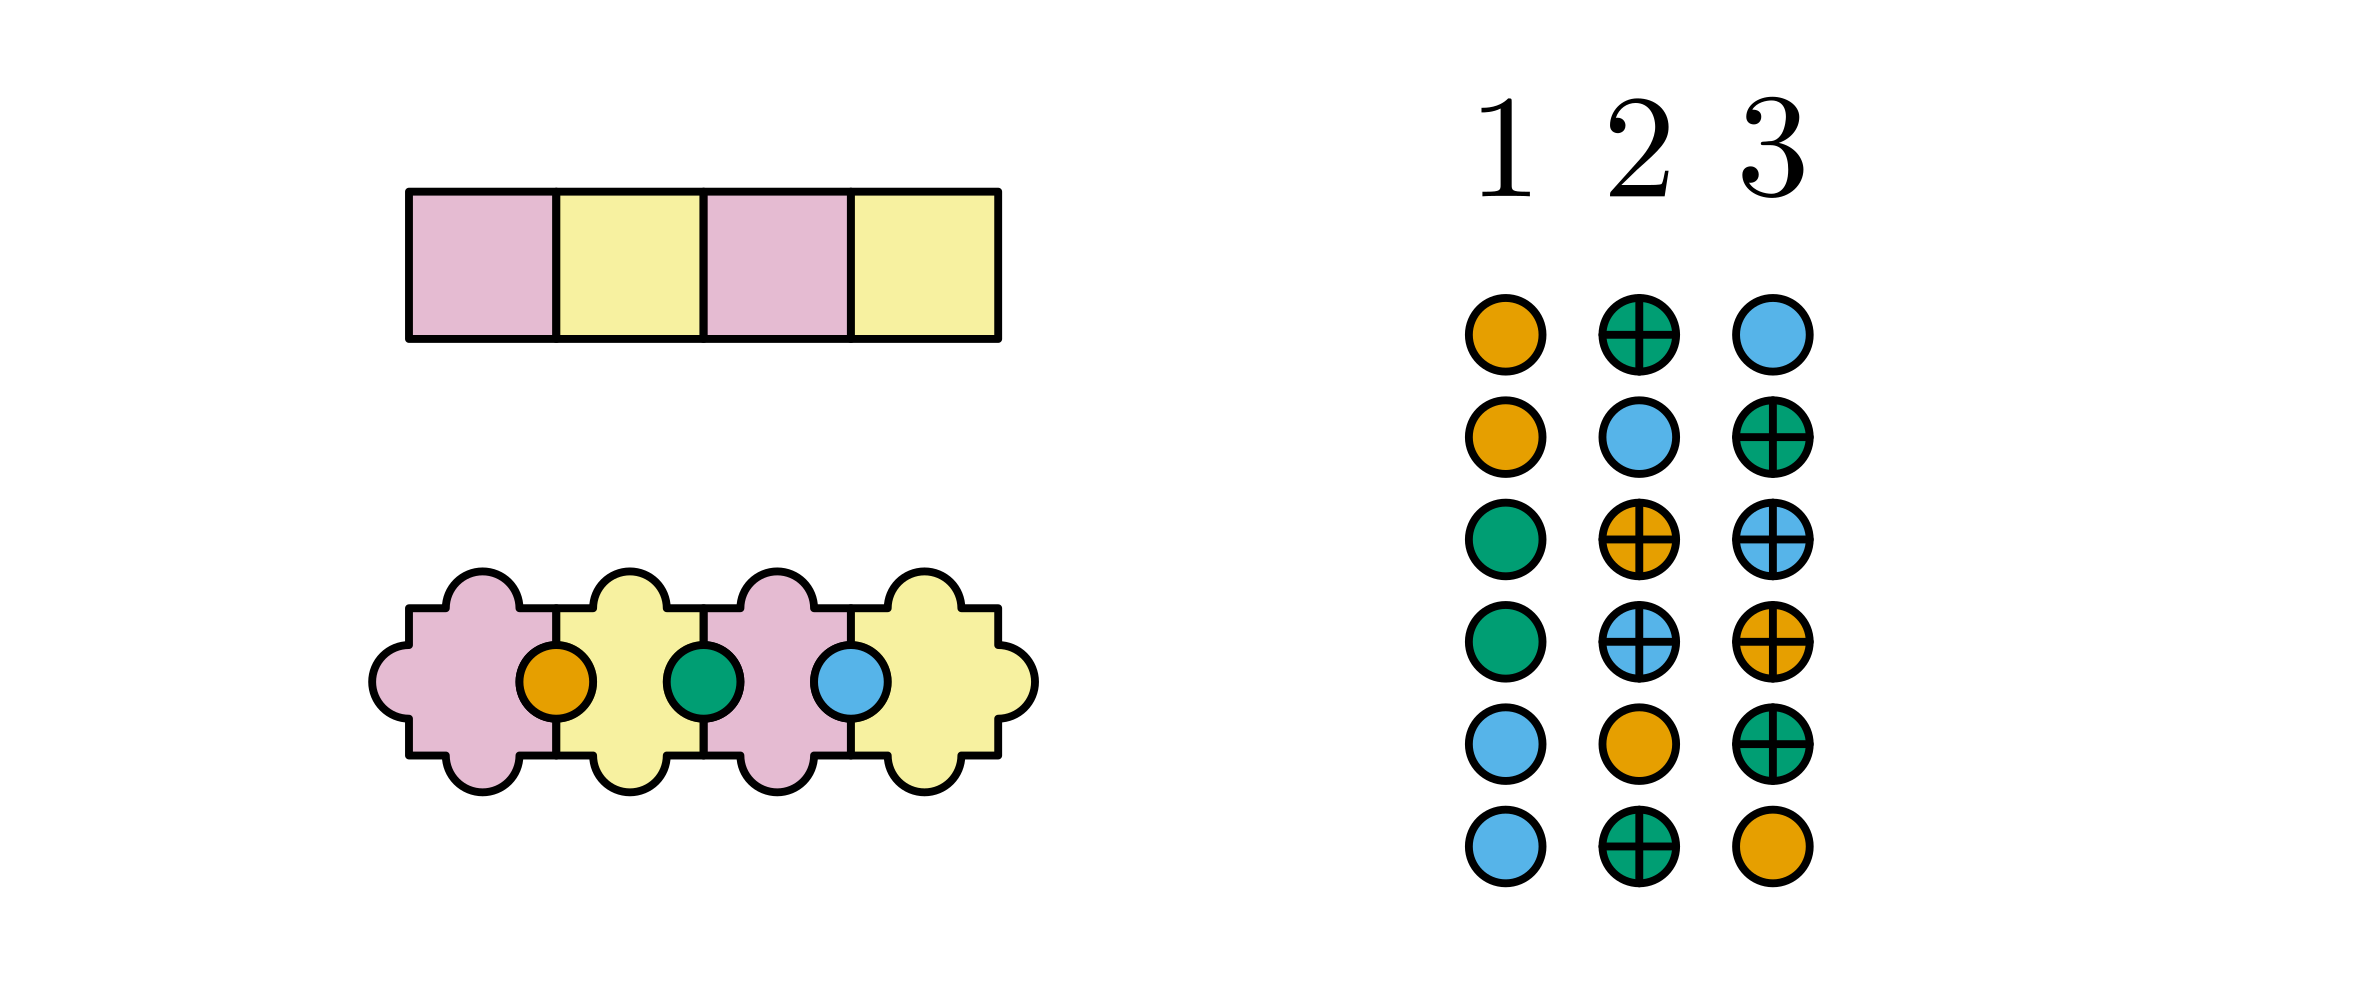
\includegraphics[width=\textwidth]{Figure 9.2.B}
\caption{The maximal independent set upon differences pairs joining hyperedges, the Boolean cells. Each row of dots demonstrates how a specific ordering may lock out certain pairings between cells.}
\end{figure}
\noindent
Due to the unique structure of Boolean random walks, each vertex in the maximal independent set is always between a positive hyperedge and a negative hyperedge. If $\chi$ determines that two hyperedges share a vertex, they exchange Boolean values. For example of the mutual pairing rule, $\chi$ is true for a specific cell's forward difference along cell face $2$ \textit{if and only if} the forward cell's backward difference along cell face $-2$ is true.

The hypergraph $G$ is defined by the hyperedges $E$ and the vertices $V$. Each Boolean cell $x$ of the system $X$ is a hyperedge in $E$, and each vertex in $V$ is a face between Boolean cells of opposing parity. A valid chording is a maximal independent set $H$, defined as a subset of $V$. To define a maximal independent set $H$, the subset $H$ and its neighbors $\gamma(H)$ equal the set $V$ \textbf{AND} the subset $H$ shares no elements in common with its neighbors $\gamma(H)$.\footnote{In set theory terms, $H \cup \gamma(H) = V$ and $H \cap \gamma(H) = \varnothing$} Each specific transition is a Boolean function $f: \mathbb B^N \rightarrow \mathbb B^N$.

We can calculate the specific Hamiltonian (energy) of a transition as $\hat \eta$, in which its relation to the relative sign $\hat \lambda$ is:
$$\hat \lambda= e^{\pi i \hat \eta}$$
The relative sign can be interpreted as the specific eigenvalue between $X_{t+1}$ and ${X_t}$. 
$$\hat\lambda(x,t) = \frac{f(x, t+1)}{f(x,t)} = \frac{X_{t+1}}{X_t} = X_{t+1} \cdot X_t$$
Note that $X_{t+1}$ and ${X_t}$ are determined or sampled states in this case, as in already decided. Due to the properties of the Boolean set $\mathbb B_{\pm}$, multiplication is the same as division. Since the specific Hamiltonian $\hat \eta$ is defined between two specific configurations, we can define it as a matrix between configurations of the state space $\mathcal X$. The state space $\mathcal X$ is the ordered collection of possible system configurations $\mathcal X = (\hat X_1, ..., \hat X_\theta).$

Let $\hat X_i$ refer to a configuration eigenstate from the state space $\mathcal X$. We may then define the specific Hamiltonian matrix $\hat \eta$ as:
$$\hat \eta = \ln(\mathcal X \otimes \mathcal X) / (\pi i)$$
in which $\otimes$ is the outer product. The rationale for the convention to divide by $\pi i$ as opposed to $2 \pi i$ is explained in \textit{\S 11.5 Boolean Thermodynamics}.

Any specific configuration eigenstate $\hat X_i$ has a decomposition into a weighted sum of its harmonic eigenstates as given by the matrix indicator function $\mathbb{I}_{(i, i)}$:
$$\mathbb{I}_{(i, i)} = \Phi c_i \Lambda \Phi^{-1} \iff c_i \Lambda = \Phi^{-1} \mathbb{I}_{(i, i)} \Phi$$
The indicator matrix $\mathbb{I}_{(i, i)}$ has a value of $1$ on the $i$-th row and $i$-th column of the matrix, and is $0$ otherwise. The constant $c_i$ is a diagonal matrix that multiplies with the diagonal matrix of eigenvalues $\Lambda$, thus constants $c$ are a sort of ``phase modifier'' for the eigenvalues $\lambda$ . This means that $\Phi c_i \Lambda \Phi^{-1}$ produces the position state $\hat X_i$ with probability 1. The decomposition of the transition from configuration eigenstate $\hat X_i$ to $\hat X_j$ is likewise given by the indicator matrix $\mathbb{I}_{(i, j)}$:
$$\Phi^{-1} \mathbb{I}_{(i, j)} \Phi = c_{(i, j)} \Lambda$$
The indicator matrix $\mathbb{I}_{(i, j)}$ has a value of $1$ on the $i$-th row and $j$-th column of the matrix, and is $0$ otherwise. This constant $c_{(i, j)}$ is also a matrix that multiplies with $\Lambda$. Other possible the constants $c$ of the ``from state'' indicator $\mathbb{I}_{(i, \cdot)}$ or the ``to state'' indicator $\mathbb{I}_{(\cdot, j)}$. In these cases, the entirety of the indicated row or column has a value of $1$ and the rest of the matrix is $0$.

A conservative system $X$ of size $N$ with $k$ particles and $(N-k)$ antiparticles has a total of $\theta = {N \choose k}$ states, conservative in the sense that the particles and antiparticles only shuffle around locally. A Boolean random walk is an example of a conservative system.
\begin{figure}[H]
\centering
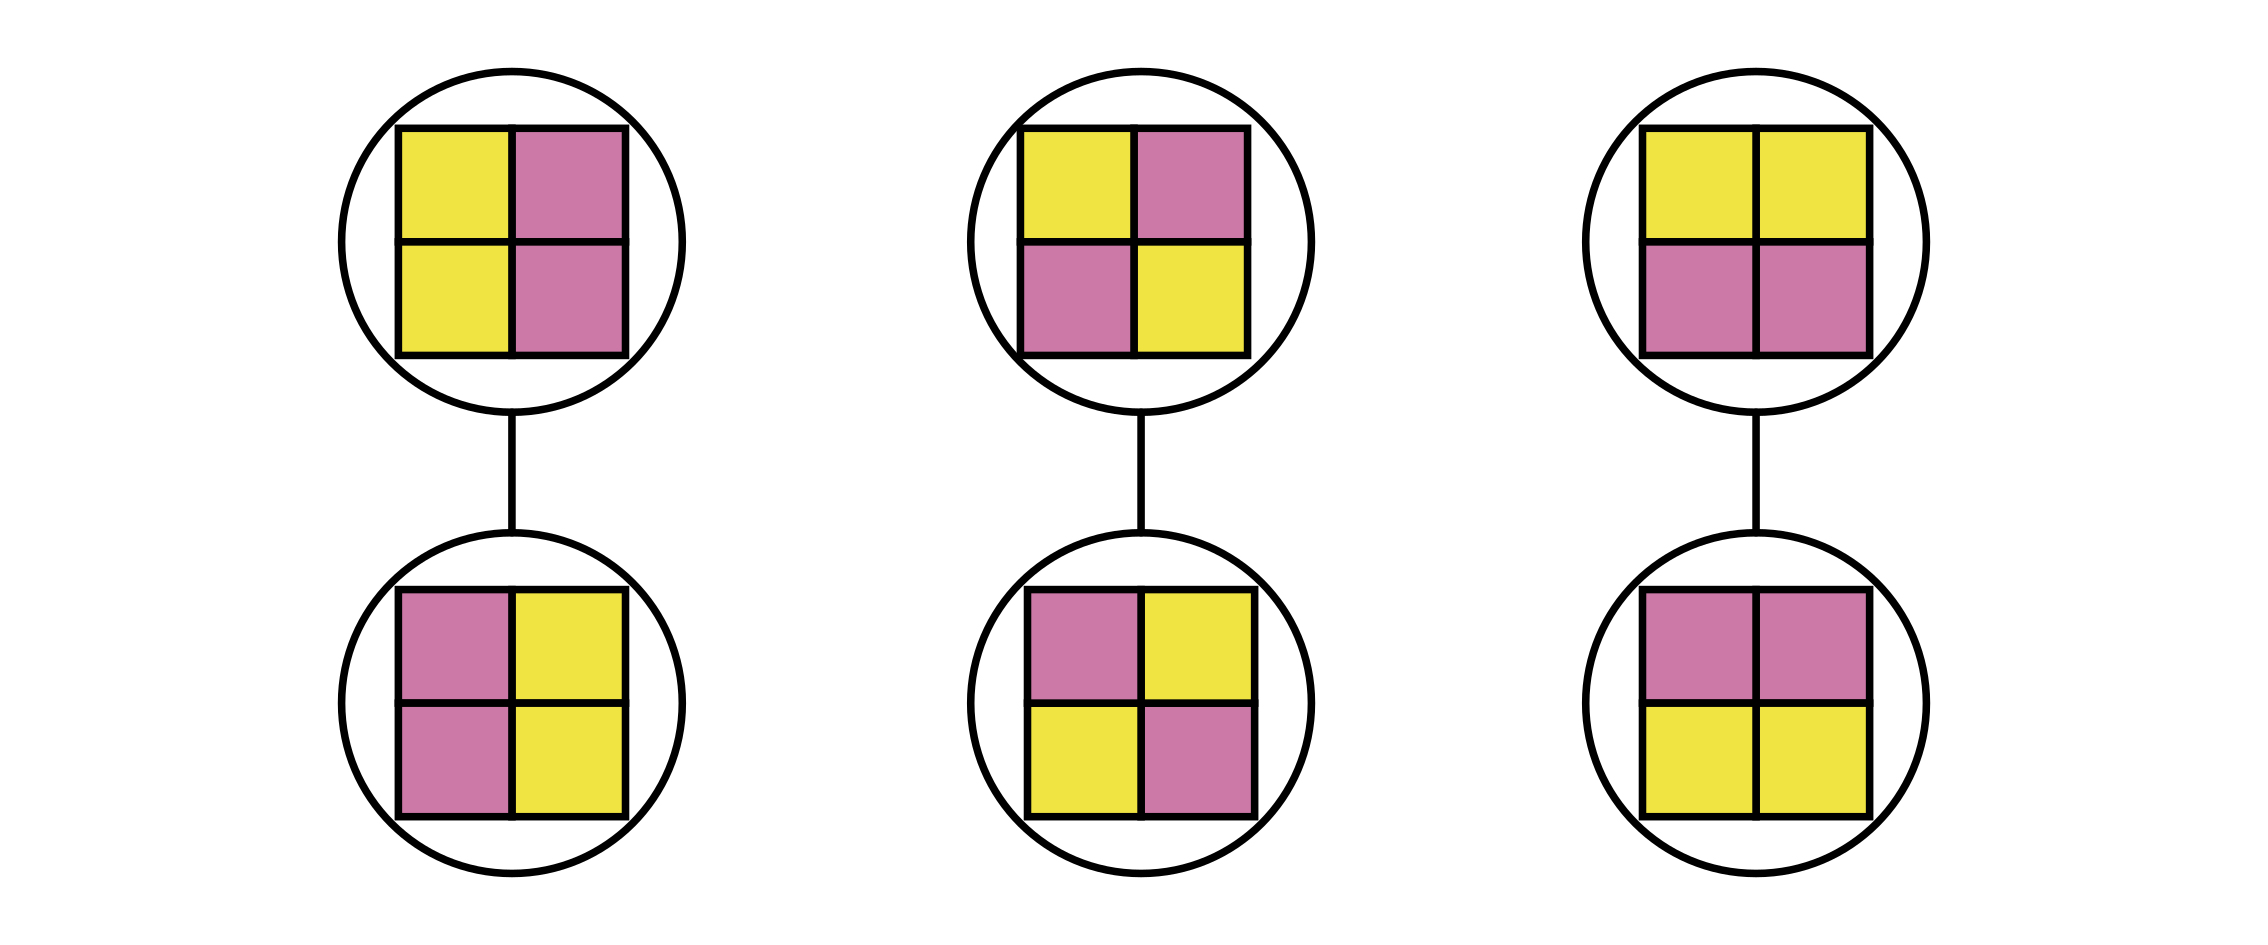
\includegraphics[width=\textwidth]{Figure 9.2.C}
\caption{All ${4 \choose 2} = 6$ possible states creates a stochastic transition matrix $P$ with $3$ communication classes}
\end{figure}
\noindent
For example, we do not have a random exterior that may change the number of particles and antiparticles. Transitions between these $\theta$ possible states may be represented using the adjacency matrix $A_{\theta \times \theta}$, in which $\theta \times \theta$ denotes the matrix size. The stochastic transition matrix $P_{\theta \times \theta}$ represents the probability of transitioning between possible \textbf{configuration eigenstates}\index{configuration eigenstate} $\hat X$ of the state space $\mathcal X$. The choose function ${N \choose k}$ grows extremely large to the point that the adjacency matrix $A$ and the stochastic matrix $P$ are effectively calculable only for small $\theta$. For example, a $\theta = {16 \choose 8}$ has an transition matrix of size $12870 \times 12870$, far larger than any computer can calculate.

The stochastic transition matrix $P$ for a system $X$ has an eigendecomposition $P = \Phi \Lambda \Phi^{-1}$ in which $\Phi$ is a $\theta \times \theta$ matrix of column eigenvectors $(\phi_1,...,\phi_\theta)$ and $\Lambda$ is a diagonal matrix of eigenvalues $(\lambda_1,...,\lambda_\theta)$. We may also prefer to use the logarithm of the eigenvalues, $\eta_j = \ln(\lambda_j)/(\pi i)$. The eigenvectors of $\Phi$ form a linearly independent basis if the system $X$ is critical, or sufficiently dense in its balance of particles and antiparticles in the case of Boolean random walks.

Recall the $1 \times 5$ bounded simple random walk system. The transition matrix $P$ is the following:
$$P = 
\begin{bmatrix}
0 & 1 & 0 & 0 & 0 \\
\frac{1}{2} & 0 & \frac{1}{2} & 0 & 0 \\
0 & \frac{1}{2} & 0 & \frac{1}{2} & 0 \\
0 & 0 & \frac{1}{2} & 0 & \frac{1}{2} \\
0 & 0 & 0 & 1 & 0
\end{bmatrix}
$$
It has an eigendecomposition $P = \Phi \Lambda \Phi^{-1}$ in which:
\[ \Phi = \frac{1}{\sqrt 5}
\begin{bmatrix}
1 & 1 & -1 & -1 & 1 \\
1 & -1 & \frac{1}{\sqrt 2} & -\frac{1}{\sqrt 2} & 0 \\
1 & 1 & 0 & 0 & -1 \\
1 & -1 & -\frac{1}{\sqrt 2} & \frac{1}{\sqrt 2} & 0 \\
1 & 1 & 1 & 1 & 1
\end{bmatrix}\]
\[
\Lambda = \begin{bmatrix}
1 & 0 & 0 & 0 & 0 \\
0 & -1 & 0 & 0 & 0 \\
0 & 0 & -\frac{1}{\sqrt 2} & 0 & 0 \\
0 & 0 & 0 & \frac{1}{\sqrt 2} & 0 \\
0 & 0 & 0 & 0 & 0
\end{bmatrix}
\]
Since it has some eigenvalue that equals $0$, the transition matrix $P$ will have no standard inverse $P^{-1}$. A critical system has no eigenvalues in which $\lambda = 0$, and there are no duplicate eigenvalues either. If we desire an inverse matrix of $P$, the best we have available is the Moore-Penrose pseudo-inverse $P^{+}$.


The state probability indicator vector $y_t = \mu(X_t)$ is a probability measure upon the configuration eigenstates $\hat X_1,...,\hat X_\theta$ of the state space. It represents the probability that the system is in a particular configuration $\hat X$ at time $t$. By convention, we define $y_0$ to be in a definite or known state, definitely in a single state, or that its entropy is $0$. As per rules of probability, the total probability of the probability vector $y$ sums to 1:
$$\sum y_t = 1$$
and each state probability is from a range:
$$(y_t)_i \in [0,1]$$
By convention, we prefer that $y_t$ is a column vector and may be derived from the initial state as $y_t = y_0 P^t$. We may alternatively use the \textbf{probability mapping matrix}\index{probability mapping matrix}:
$$\rho_t = \textnormal{diag}(y_0) P^t$$
in which $\rho_t$ is a matrix of entries of $y_0$ maps into the future at time $t$. Quantum mechanics refers to density matrices where $\rho^2 = \rho$ as pure states, thus our convention for $\rho_0$ is that it is a pure state. Summing along the columns of $\rho_t$ produces a value identical to $y_t$.


We prefer that the eigendecomposition $P = \Phi \Lambda \Phi^{-1}$ is of unit magnitude, meaning that each eigenvector $\phi$ has a Euclidean distance of $1$. These column eigenvectors $(\phi_1,...,\phi_\theta)$ have a weight associated with the Boolean \textbf{configuration eigenstates}\index{configuration eigenstate} $(\hat X_1,...,\hat X_\theta)$. Since every Boolean configuration is a valued field, we can define the harmonic eigenstates $(\hat A_1,..., \hat A_\theta)$ in the following way:
$$\hat A_{j} = \sum\limits_{i=1}^{\theta} \Phi_{(i, j)} \hat X_{i}$$
These \textbf{harmonic eigenstates}\index{harmonic eigenstate} are the also called the normal modes. We might call these the pure states or quantum states of momentum in physics, but momentum would be a misnomer since we never observe momentum like a particle.

A Boolean random walk system $X$ with transition matrix $P$ always has harmonic eigenstates $\hat A_1$ and $\hat A_2$:
\begin{figure}[H]
\centering
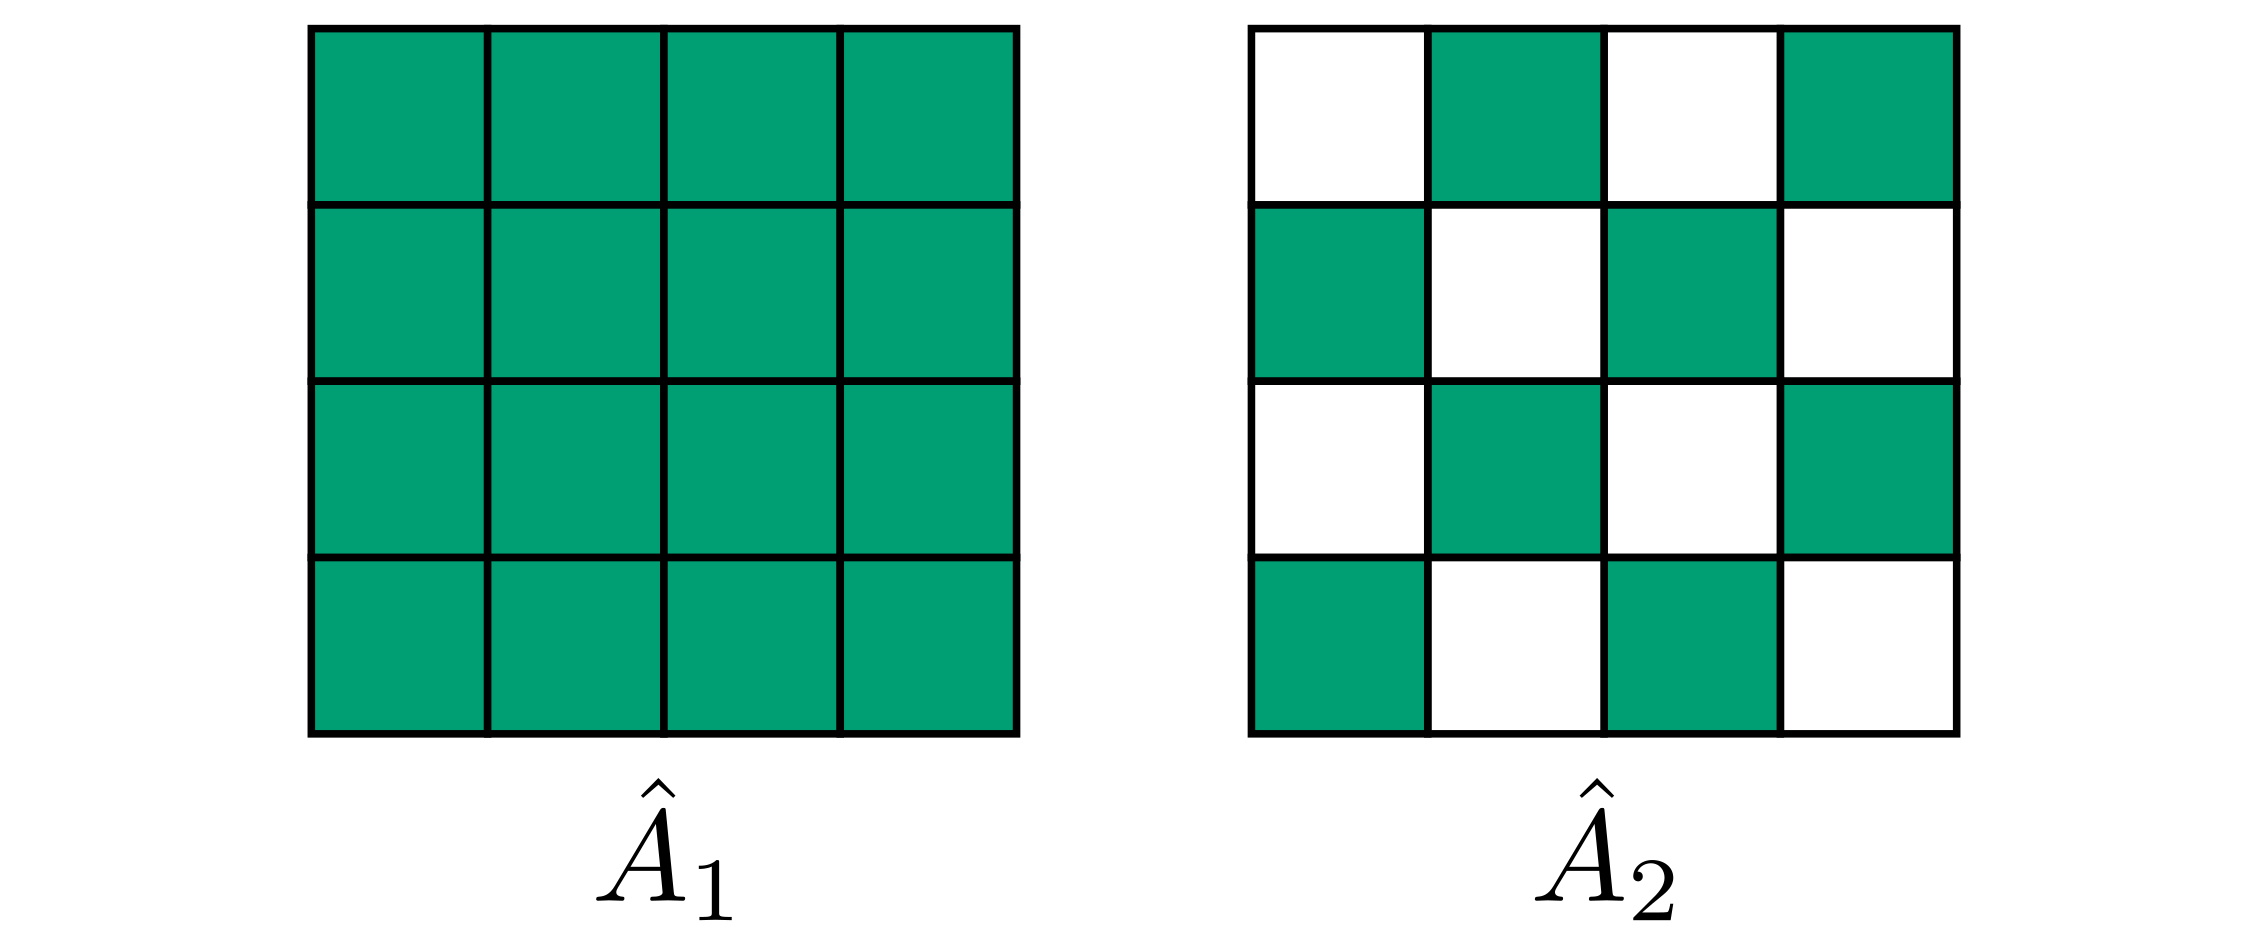
\includegraphics[width=\textwidth]{Figure 9.2.D}
\caption{The uniform and checkerboard modes}
\end{figure} \noindent
The uniform eigenstate $\hat A_1$ and the checkerboard eigenstate $\hat A_2$ corresponds to eigenvalues of $\lambda_1 = 1 = e^{0}$ and $\lambda_2 = -1 = e^{\pi i}$ respectively. Any specific state is either an even or odd state, indicated by the phase modifier $c$ for the checkerboard mode. Thankfully, linear Boolean sequences such as:
$$\mathcal X = (000, 001, 010, 011, 100, 101, 110, 111)$$
are already ordered according to parity. Since a Boolean random walk is $2$-periodic, we may also designate one state as even and the states it walks to as odd.

The Boolean representation of the natural numbers $(0,...,\theta-1)$ of our state space $\mathcal X$ has dichromatic symmetry with respect to the transiton function and only if our transition function has dichromatic symmetry with respect to local cell probabilities.\footnote{See \textit{Figure 11.21}} Chiral states are states that are not symmetric with respect to rotation, mirror, or inversion. This means more ``versions'' of the state exist in the state space $\mathcal X$. Chiral states should have isomorphic rows with respect to rotational, mirror, and of course dichromatic symmetry. There should be no more than $2*2*d$ states of similar weight for any chiral state $X$:
\begin{figure}[H]
\centering
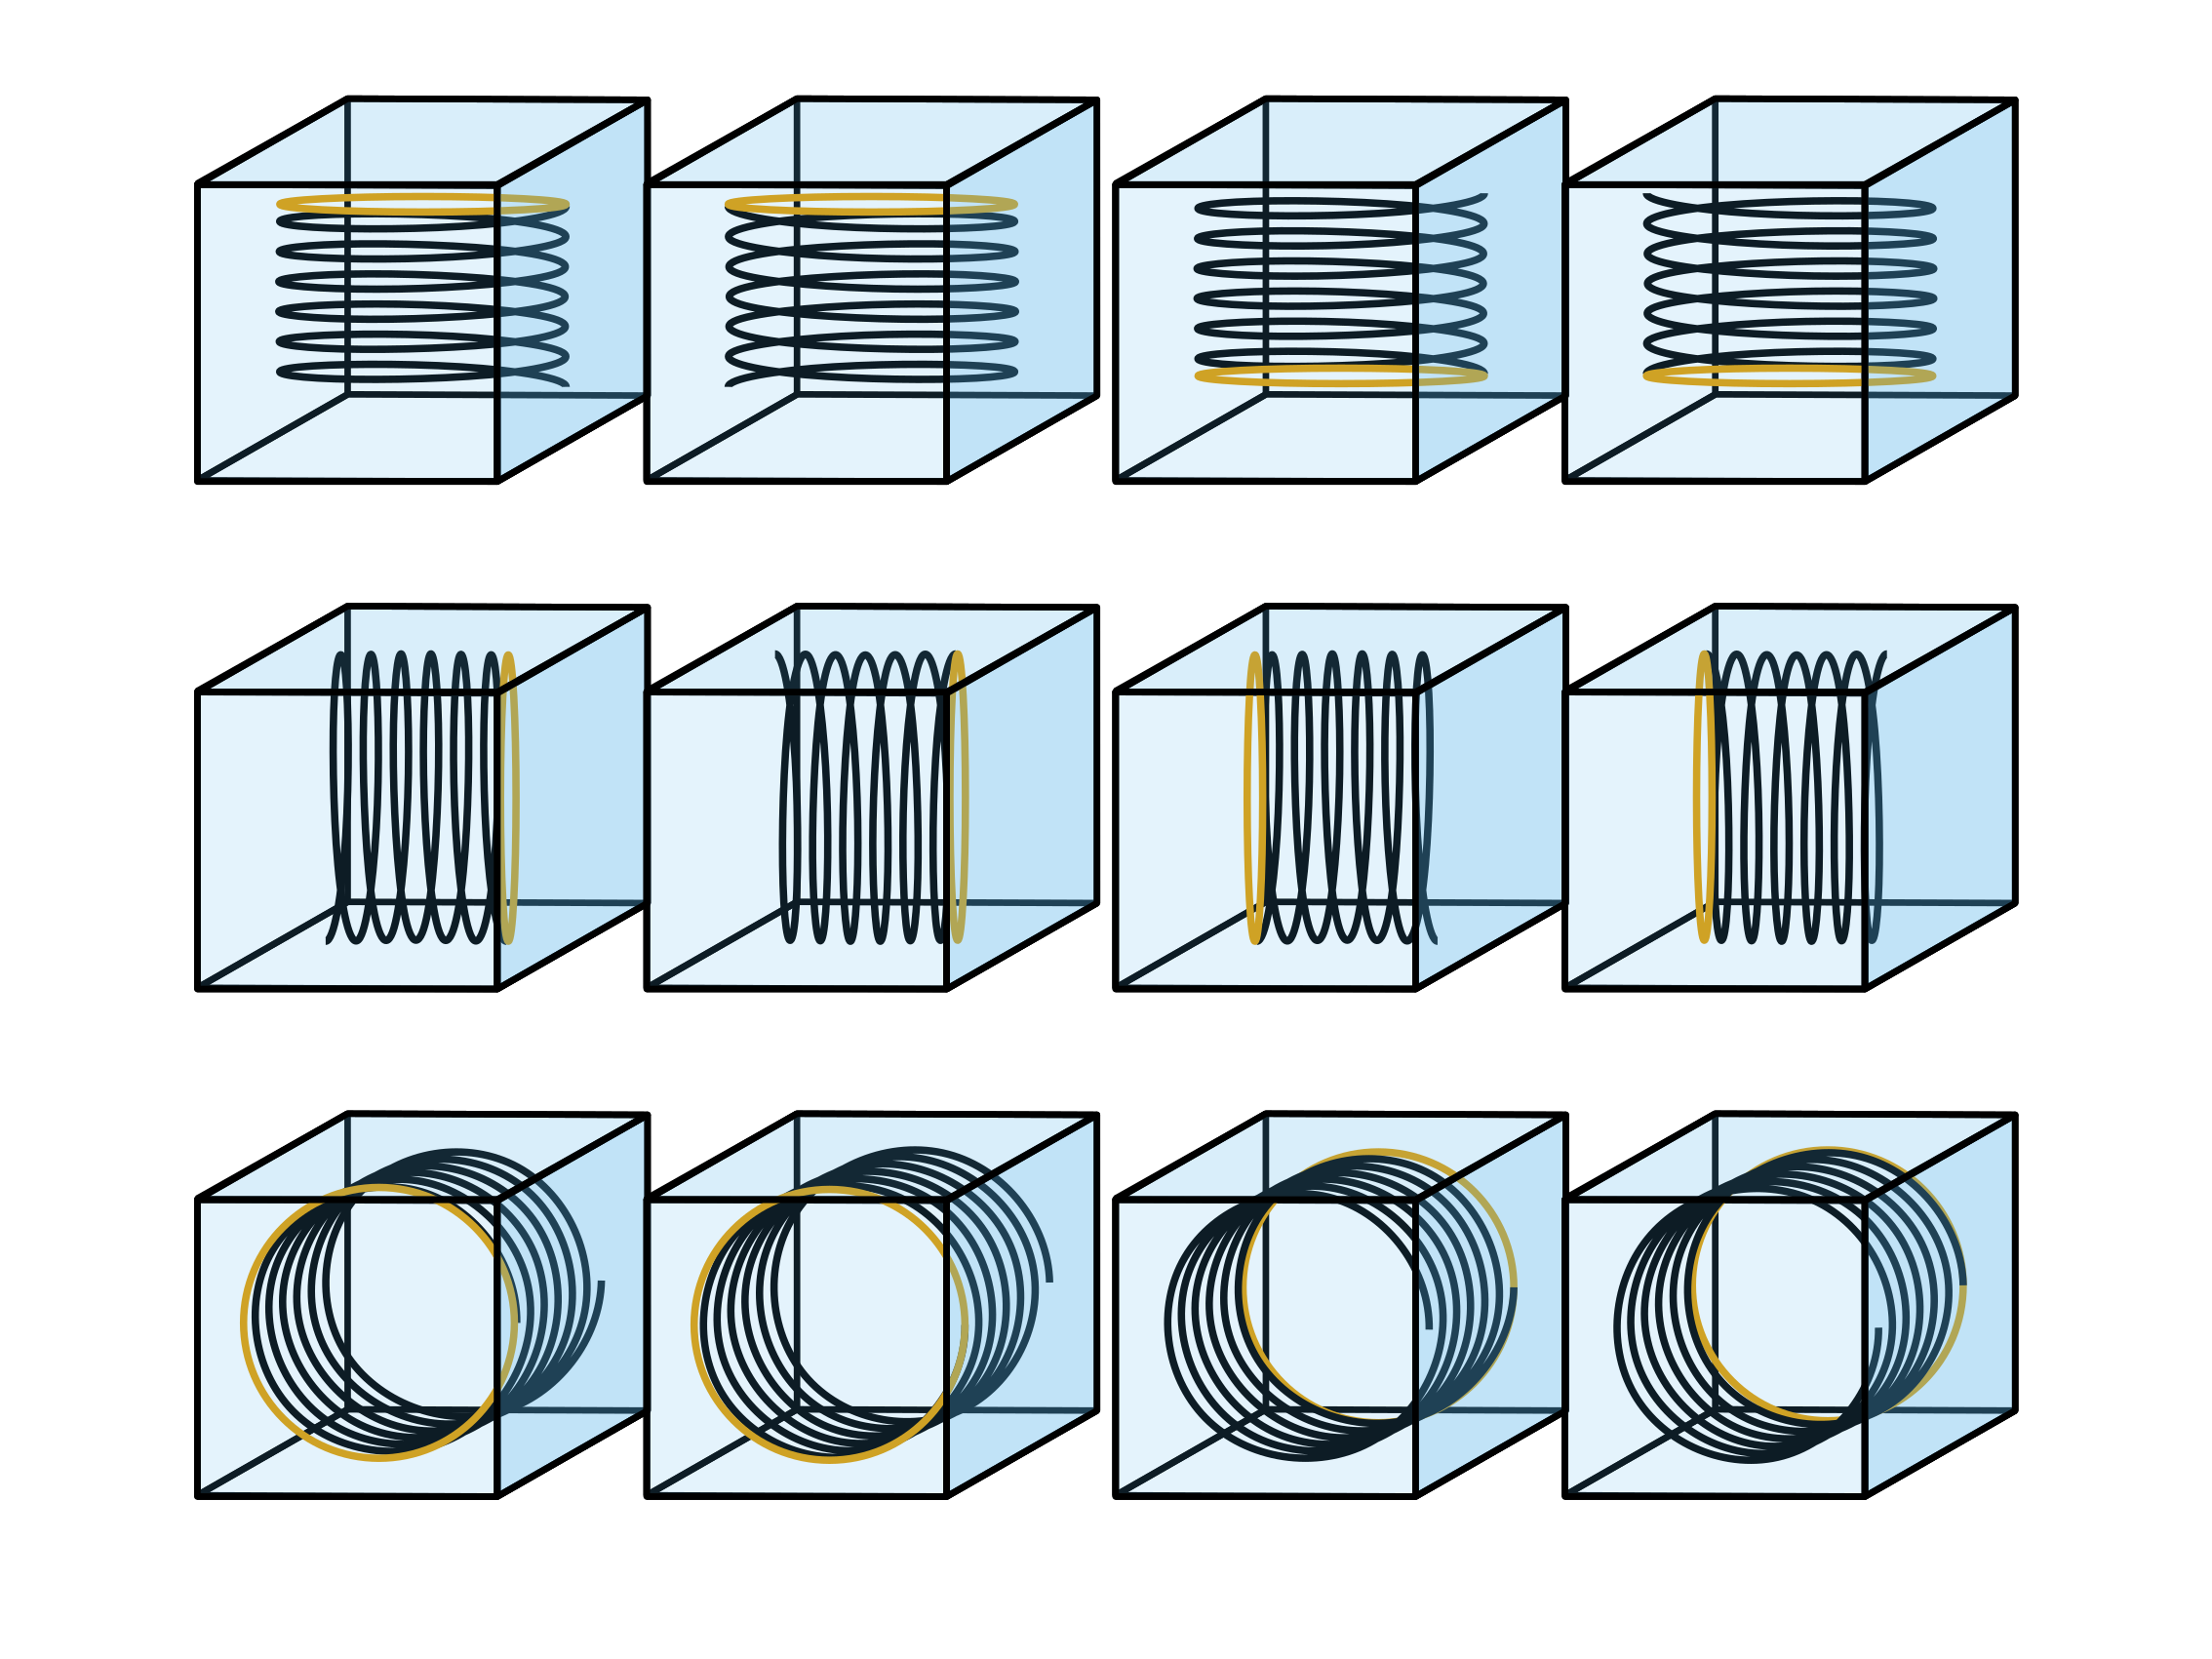
\includegraphics[width=\textwidth]{Figure 9.2.E}
\caption{Chiral states in 3D have $2*2*3=12$ versions}
\end{figure} \noindent
Here, a chiral state represented by a spring has $12$ possible states of similar entropy $\times$ parity. These states appear identical in the stochastic matrix $P$, yet the matrix $P$ is implied to be a full rank matrix. In contrast, a checkerboard state only has $2$ versions due to rotating, mirroring, and inverting Booleans corresponding to the same transformation.

The state space of a system $X$ is denoted by $\mathcal X$, and we shall denote its graph without probability measure as $\mathcal X_G$. As our size for $X$ increases, it grows to include some representation every computable Boolean function. As discussed in \textit{\S 7 Graph Theory}, the transition function $f$ we are referring to is the functionally omnipotent graph in which all possible chordings are considered the same transition $f: X_i \rightarrow X_j$. The transition matrix $P$ provides probability weights to all these mappings. 

This brings us to our paradox. Let $X_\omega$ refer to a system of infinite size such that |$n_i| = \aleph_0$ for all dimensions $i \in (1,...,d)$, and finite subsets contain every computable function of that finite size. The infinite repeating pattern $X_\Omega$ must transition to and from a state that has every computable function. Are there infinitely many states that do so or does there only exist a single state that contains every computable function that transitions into itself? Such as question may be undecidable. If the state space graph $\mathcal X_G$ only contains one vertex and one edge, then it is a monocyclic or autocyclic graph:
\begin{figure}[H]
\centering
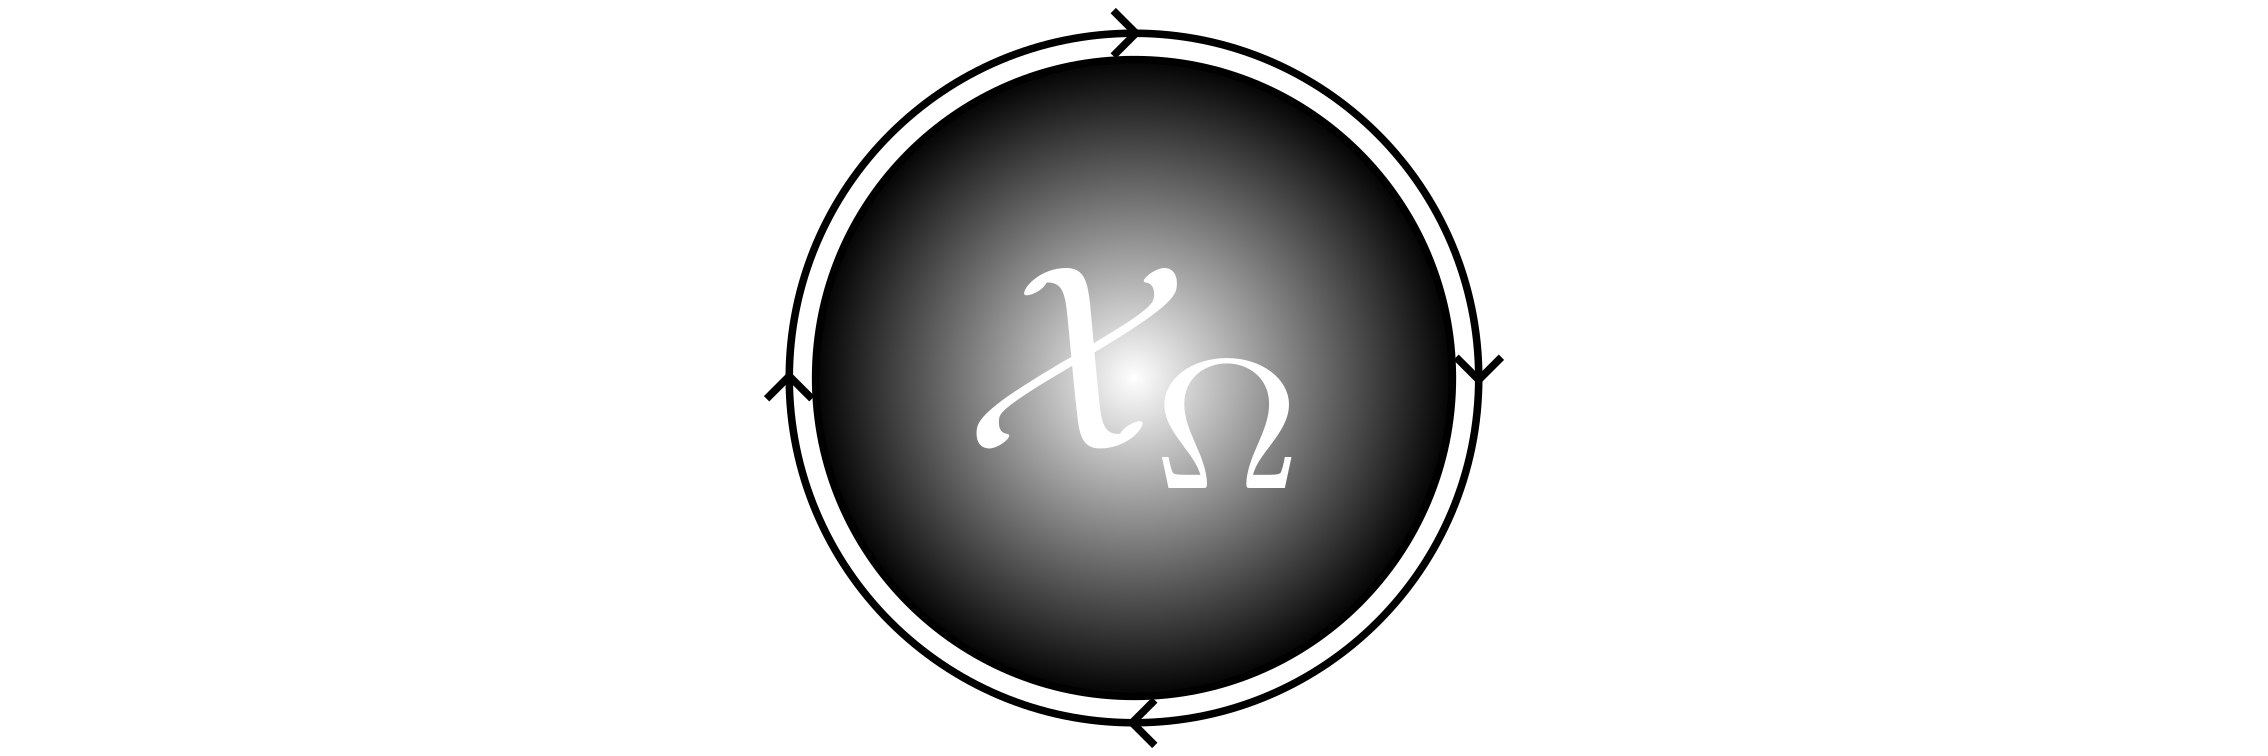
\includegraphics[width=\textwidth]{Figure 9.2.F}
\caption{An infinite system executing infinite copies of every computable function can only transition into itself}
\end{figure} \noindent
There must be an infinite amount of copies of every subsystem, an infinite number of copies of specific arrangements of subsystems that make larger systems, and it must repeat this process for an infinite amount of time steps. Each finitely measured system has a countably infinite number of copies, and each specific transition has a countably infinite number of occurrences.

Allow me to simplify the metaphysical argument. Suppose we have a system $X_0$ that randomly transitions in time. At each time step, each element from the set of integers $\mathbb Z$ is assigned a Boolean value according to a fair coin flip. If we say that two states are the same if they are isomorphic with respect to translation, then is the cardinality of the state space $\aleph_0$ or $1$? Consider the Rado graph, a graph which contains every possible graph as its subset a countably infinite number of times. However we attempt to construct a Rado graph, there is only \textit{one possible} Rado graph. In that sense, the time advancements of our random Boolean universe also only advance to the same state, running in circles.

The infinitesimal number $\varepsilon$ is the smallest number that is closest to $0$ that is not itself $0$. Likewise, the infinity $\omega$ is given by $\omega = \varepsilon^{-1}$. These give us constructions for the hyperreal numbers, but we need them more for their usefulness in the calculus of finite differences.\footnote{A moderately useful idea is to take $\omega$ to be our hyperreal infinity number such that $\omega = \infty$. Then we might say that $\ln(0) = \ln(e^{-\infty}) = \ln(e^{-\omega}) = -\omega$} Let $\Delta_t(\varepsilon)$ correspond to the forward difference operator with respect to variable $t$ of step size $\varepsilon$. The difference relation:
$$\frac{\Delta_t(\varepsilon)}{\varepsilon} (1 + \eta \varepsilon)^{\frac{t}{\varepsilon}} =
\frac{\Delta_t(\varepsilon)}{\varepsilon} e^{\log(1 + \eta \varepsilon)\frac{t}{\varepsilon}} = 
\eta e^{\log(1 + \eta \varepsilon)\frac{t}{\varepsilon}}
$$
means that $2^t$ is the eigenfunction of the forward difference operator $\Delta$:
$$\Delta_t 2^t = 2^t$$
for $\eta = \varepsilon = 1$. These ideas are key to help us relate concepts of continuum calculus and umbral/discrete calculus. For example, integrals instead become summations if we understand $\Delta_t 2^t = 2^t \iff 2^t = (\Delta_t)^{-1} 2^t$ via the equation:
$$(\Delta_t)^{-1} = \sum\limits_{n=1}^{\infty} (B_t)^n \implies (\Delta_t)^{-1} \Delta_t f(x,t) = \sum\limits_{n=1}^{\infty} (B_t)^n \Delta_t f(x,t)$$
So the present value of the function $f(x, t)$ is the summation of its infinite series of backshifted forward differences. Quite the mouthful. How is this relevant for Boolean mechanics? The present state of a system $f(x,t)$ can be derived from an infinite series of changes, assuming they exist. Due to the Markov property of state spaces, we only need until we have some piece of data to condition upon.

The forward difference operator $\Delta_t(1) = \Delta_t$ has another possible result if you change $\eta = -1$:
$$\eta e^{\log(1 + \eta \varepsilon)\frac{t}{\varepsilon}} = -1 \cdot 0^t$$
This seemingly nonsensical result is nonetheless relevant to interpretations of Boolean statistical mechanics. We might look and consider that if we use the backwards difference operator instead via $\Delta_t(-1)$. Thus, the function $\Delta_t(-1) 2^t$ corresponds to eigenvalue $\eta = -1$: the function $2^t$ represents bit-flip pairing while the value $-1 = e^{1 \pi i}$ represents rotation. Conversely, $\Delta_t(-1) 0^t$ corresponds to eigenvalue $\eta = 1$: the function $0^t$ represents isolation (no pairing) while the value $1 = e^{0 \pi i}$ represents a null rotation.

Subtle interpretations like this should perhaps not be taken as rigorous explanations of Boolean statistical mechanics, but they are alternative perspectives worth considering. At its core, Boolean statistical mechanics proposes a simple idea using a breadth of undergraduate mathematics and statistics. The question is which mixture of notations of different branches of mathematics makes the concepts easiest to grasp. 

\section{Primary Rules and Rule Duality}
The primary rules of a Boolean mechanical system $X_t$ ensure that it behaves similarly to independent random walks for sparse systems and behaves identically for particles and antiparticles for time advancements:
$$B_t^{-1} X_t = -B_t^{-1} (-X_t)$$
Boolean random walks grants insight for the exact entropy of ``balls in a box'' model as well as a definition of temperature. However, we lose the ideal of a cellular automaton that only depends on its immediate neighbors per cell due to relying on maximal independent sets for transitions.
\begin{figure}[H]
\centering
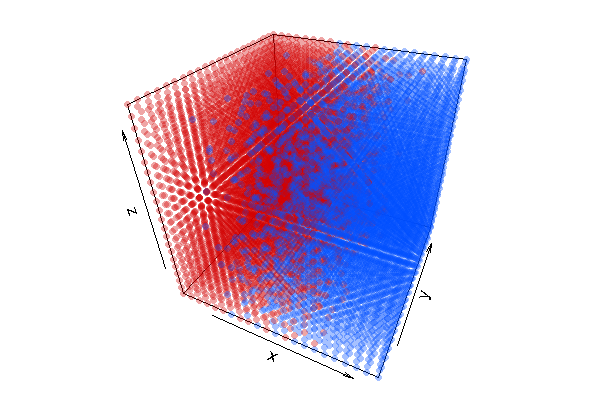
\includegraphics[width=\textwidth]{Figure 9.3.A}
\caption{A 3D Boolean random walk with high entropy in the center and low entropy at the edges}
\end{figure} \noindent

These are the primary rules of a Boolean random walk system $X_t$:
\begin{enumerate}
\item Measure Preserving: The number of particles $k$ and the number of antiparticles $(N-k)$ in system $X-t$ are the same for all time steps $t$.
\item Identical Particles: Particles are indistinguishable from particles, and antiparticles are indistinguishable from antiparticles. They are not unique, lacking identity at the individual level.
\item Differentially Permissive: Particles and antiparticles are permitted to exchange if adjacent due to differences in charge $+1$ and $-1$ respectively. Particles may not exchange with particles, likewise for antiparticles, due to a charge difference of $0$.
\item Speed of Light: No particle or antiparticle may travel more than length $1$ per time step $1$, and this corresponds to one bit flip per time step per cell.
\item Difference Exhaustive: At each time step, a system must exhausted all finite-differences that are permitted until each particle/antiparticle is paired or isolated from partners.
\item Charge Symmetric: $e^{\frac{\partial}{\partial t}} X_t = -e^{\frac{\partial}{\partial t}} (-X_t) = X_{t+1}$
\end{enumerate}
At no point here have we made explicit reference to a random walk, and yet they are bisimulative to them for $k=1$. A bisimulation is a relation that states two systems are bisimilar if they imitate each other's moves (or probability measures) for a given game. Outside observers cannot distinguish between the two systems by observing results alone.

The rules from the perspective from of particles and antiparticles that may not travel faster than the speed of light per time step is dual to the cellular automaton perspective: instead of perceiving particles in a diffusion equation, it considers cells or positions of the lattice that do not move. Cells are assigned a charge, and they must permissive-exhaustively pair to adjacent cells of opposing charge. In simpler terms, a maximal independent set must be chosen upon vertices and edges, each vertex is between two cells of opposing charge and each (hyper)edge is a cell assigned a Boolean value.

The cell perspective is not as natural to us because objects are defined by their seemingly obvious boundaries. Even though particles and antiparticles occupy cells, we are not apt to see the canvas behind the paint nor the void around the quark. To understand everything, we must first understanding nothing. Despite Boolean random walks being rather simple, it was not discovered because we perceive the random walker and not the random empty. It is a fundamental flaw of human cognition to perceive the foreground and not the background.

\section{Computational Indistinguishability}
\textbf{Computational indistinguishability}\index{computational indistinguishability} means that two probability distributing are difficult to tell apart except for some small probability. Distinguishability $\delta(n)$ between two sample generators $D_n$ and $E_n$ is defined as:
$$\delta(n) = \Big| \underset{x \leftarrow D_n}{P}[A(x) = 1] - \underset{x \leftarrow E_n}{P}[A(x) = 1] \Big|$$
Computational indistinguishability is achieved when $\delta(n)$ is small and does not improve as $n \rightarrow \infty$. The distinguishing algorithm $A$ returns an arbitrarily small $\delta(n)$ if $D_n \approx E_n$. This is a weaker condition than a bisimulation, in which the two different algorithms have identical output distributions.

Computational indistinguishability is fundamental to what it means to classify objects. When we are defining a macroparticle in Boolean statistical mechanics, each microstate in the macrostate should have a similar distribution after some finite amount of time. Ideally, a macroparticle class $G$ also behaves similarly under two different media $m_1$ and $m_2$. 

Let $\partial G$ be the boundary of a macroparticle class, and let each $g \in G$ be of the same size and shape. For $g \in G$, consider the following scenario:
\begin{figure}[H]
\centering
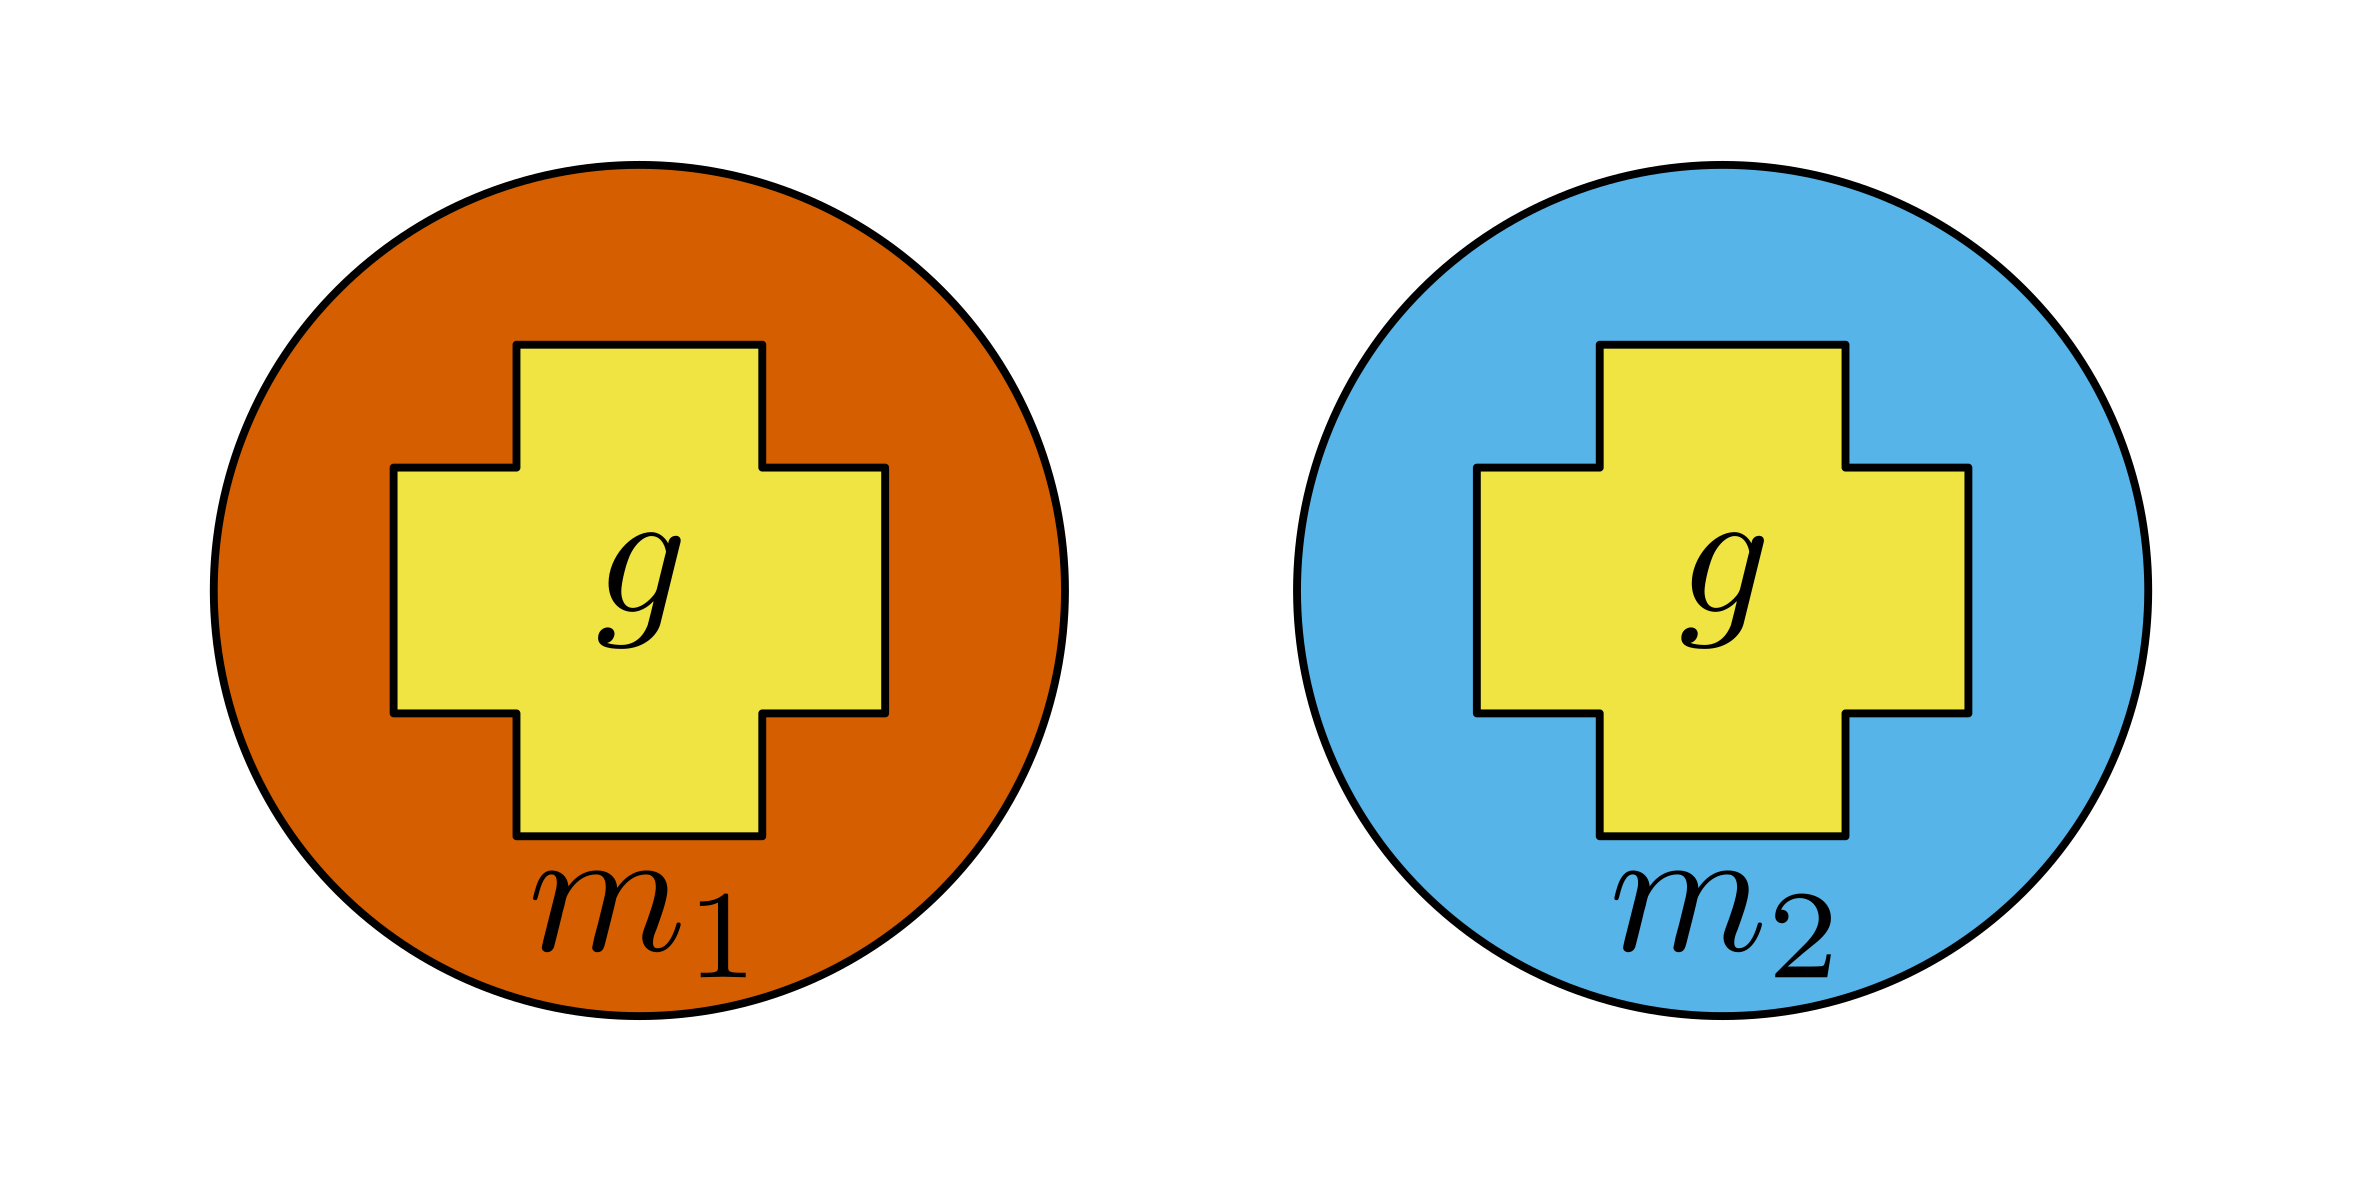
\includegraphics[width=\textwidth]{Figure 9.4.A}
\caption{A single state $g$ in two different surroundings $m_1$ and $m_2$}
\end{figure}
\noindent
A specific configuration of the macroparticle $g$ is placed in two different media $m_1$ and $m_2$ that stretch out to infinity. Is the transition from of $G_{t}\cup \partial G_{t} \rightarrow G_{t+1}$ identical across a probability distribution of media $M = m_1,...,m_k$? 

A physics example would be to ask how water behaves differently on the core or surface of an ice planet. At the core, high temperature water would still be solid ice under the cumulative pressure of the material above it. In our mind's distinguishing algorithm, we consider ice as a solid state of water, but we do not consider free moving hydrogen ions and oxygen ions to act similarly to water. Why, and under what metric?

Consider the inverse prediction problem. Given that you have two specific outputs $g_1, g_2$ from a transition $G_t \rightarrow G_{t+1}$, can you predict the media $m$ that produced them? Can you generate two media distributions $M_1$ and $M_2$ that produce some specific resulting transition? What is the computational complexity of finding some approximate solution? Consider the boundary cells around $G$, denoted as $\partial G$, and assume that $G$ is a convex shape. The boundary cells $\partial G$ is the subset of $M$ adjacent to $G$:
\begin{figure}[H]
\centering
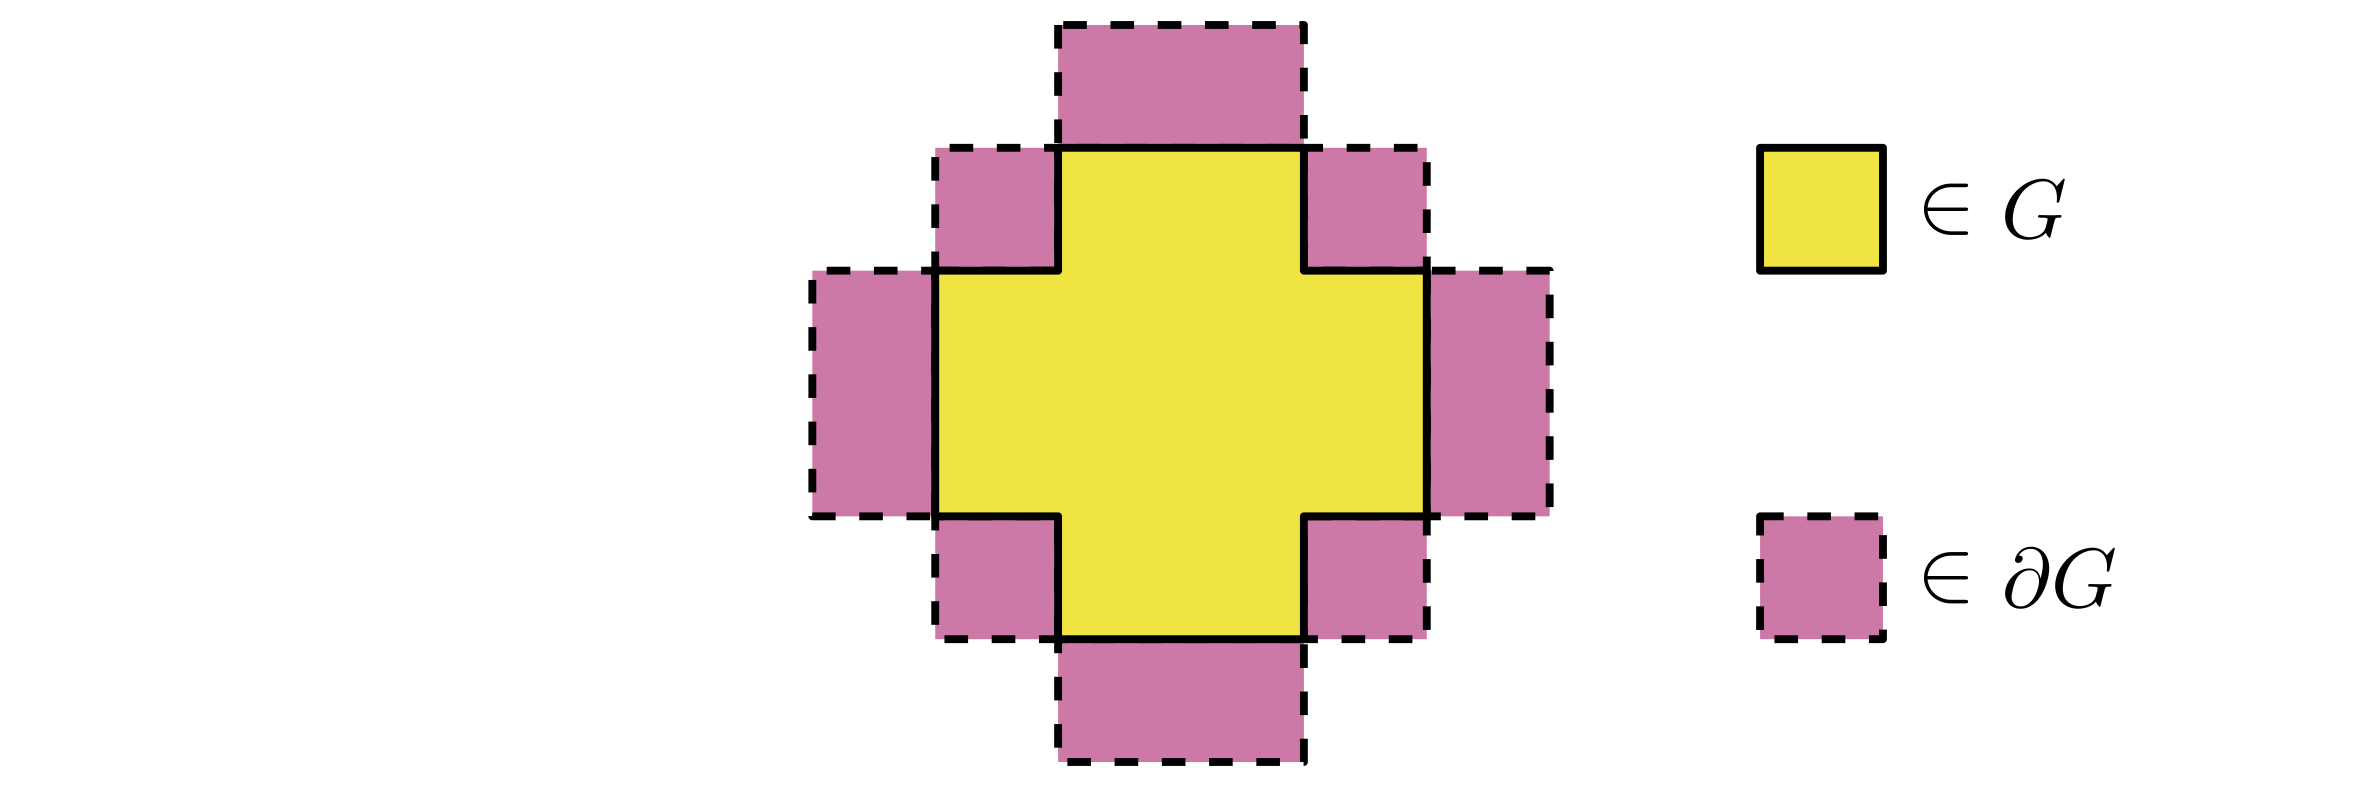
\includegraphics[width=\textwidth]{Figure 9.4.B}
\caption{A visualization of the immediate boundary of $G$}
\end{figure}
\noindent
Even for a Boolean random walk with statistical dependence upon distant cells, the nearest cells have the most influence upon the future distribution of $G_t$. 
\begin{figure}[H]
\centering
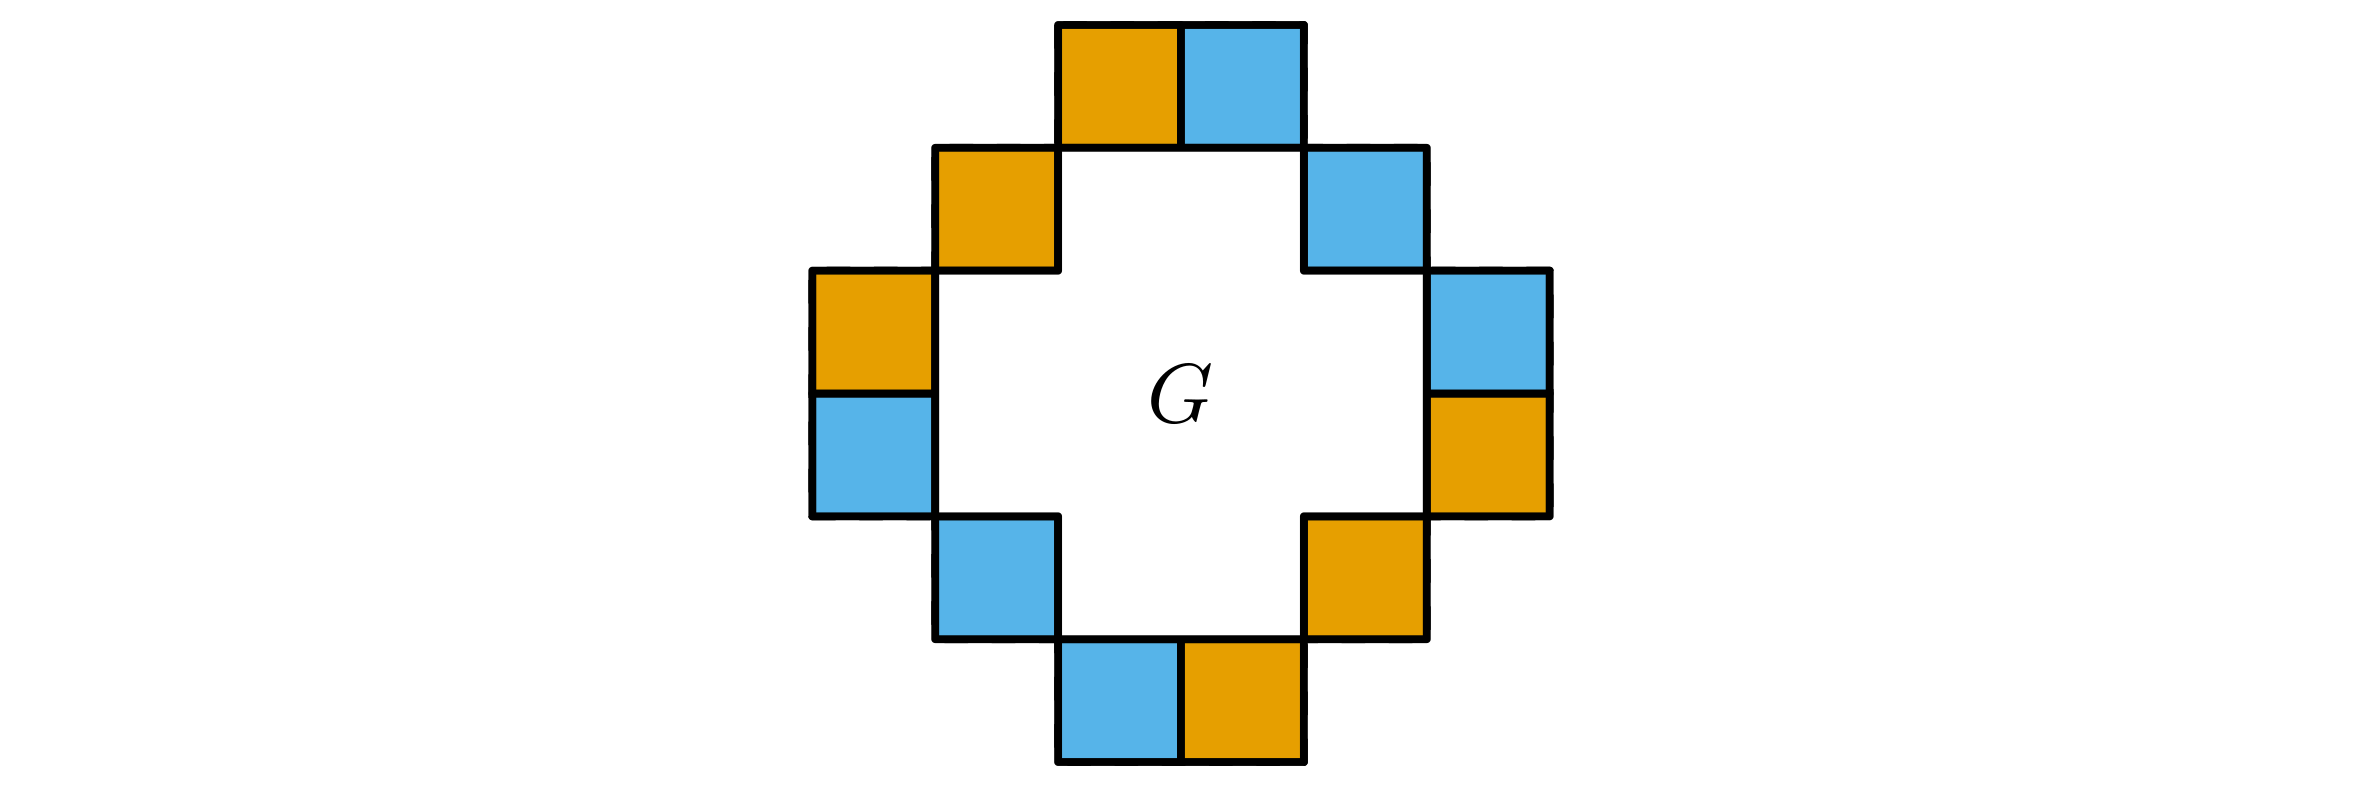
\includegraphics[width=\textwidth]{Figure 9.4.C}
\caption{The immediate boundary $\partial G$ determines transitions}
\end{figure} \noindent
Even if $G$ is influenced by the totality of $M$, $G$ may only exchange with its interior and its immediate neighbors $\partial G$. We discuss more about a theory of macroparticles in \textit{\S 11.7 Macroparticle Creation and Annihilation}.

If we restrict the scope of our problem to $M = \partial G$, then we only need to obtain samples of $M$ from a much larger simulation. If we consider the $2d+1$ shifts of some $G$ via the shift operator $e^{\frac{\partial}{\partial x}}$, the null shift $e^{\frac{\partial}{\partial x_0}}$ and the postive/negative dimensional shifts $e^{\pm \frac{\partial}{\partial x_1}},...,e^{\pm \frac{\partial}{\partial x_d}}$, then we may obtain the eigenclass $G_{\varnothing}$ given some boundary distribution $\partial G = M$ using the following formula:
$$p_{G_{t+1}}(G_{t+1} = g_j) = \sum\limits_{j=1}^\theta \sum\limits_{i=-d}^d p_{G_t}(G_t = g_j) p_X(X=x_i) e^{\frac{\partial}{\partial x_i}}$$
$$p_{G_{t+1}}(G_{t+1} = g_j) = p_{G_t}(G_t = g_j)$$
If there exists no shift distribution $e^{\frac{\partial}{\partial}}$ which returns the same distribution for $G$, then $G$ has no eigenclass for a given boundary media distribution $\partial G = M$. Under our improper notation:
$$e^{\frac{\partial}{\partial x_{(-d)}}} = e^{-\frac{\partial}{\partial x_{d}}}$$
means a unit shift in the negative direction of a dimension.

In other words, $G$ must be the eigenfunction of the shift operator given a medium $M$. The probability distribution of $G_t \rightarrow G_{t+1}$, should have the similar probability densities under random walk-like shifts in space. This is because we are assuming that the set of states that define a macroparticle should behave similarly to an unbiased random walk. Since we have not defined the concept of ``movement'' for macroscopic objects in a Boolean random walk, the best we can do is consider a configuration probability distributions behaving similarly under some random walk-like shift distribution.

In order to properly simulate the boundary distribution $\partial G$, we must introduce \textbf{phantom zeroes}. A \textbf{phantom zero}\index{phantom zero} is an element of $\partial G$ that bit flip with $\partial (G \cup \partial G)$. Since the cell at the exterior boundary is performing a switch at its further exterior, this means that the cell of $\partial G$ cannot form a particle-antiparticle pair with a cell from the interior $G$. We can simulate phantom zeroes by consider the overall average probability of a bit flip:
$$\frac{1}{N} \sum\limits_{x \in X} p(e^{\frac{\partial}{\partial t}} = -1)$$
This method is inherently flawed: a true phantom zero is not a statistically independent distribution across the boundary. Let us assume that we are working with a critically dense Boolean random walk ($k = N-k$). We should instead empirically sample $\partial G$ from an extremely large Boolean mechanical system, and we should record cells of $\partial G$ that are unable to switch into $G$ or $\partial G$ as phantom zeroes. We now have a Monte Carlo simulation method for obtaining a $\partial G$ boundary noise distribution.

Our choice of shift distribution $X$ corresponds to a \textit{random walk} of a particle in $d$-dimensions. The expected velocity of the macroparticle class $G$ that we wish to assign:
$$\sum\limits_{i=-d}^d x_i \cdot p_X (X = x_i) = \mathrm{E}(X) = \mu_X$$
The absolute value of the expected velocity of a macroparticle class $G$ may not exceed the speed of light, $\mathrm{E}(X) \leq 1$ due to diagonal movement. Likewise, the variance of the velocity distribution is given by:
$$\sum\limits_{i=-d}^d (x_i \cdot p_X (X = x_i)- \mu_X)^2 = \mathrm{Var}(X) = \sigma_X^2$$
in which our variance is also restricted by $\mathrm{Var}(X) \leq 1$. The main issue with this approach is the \textit{subjectivity} or \textit{arbitrariness} that it imposes upon us as mathematicians. Why should we use one shift distribution and not the other?

We should be interested in shift distributions with an average movement of $\mathrm{E}(X) = 0$ since we are trying to find the eigenclasses $G_{\varnothing}$ for a (macro)particle in a box. It only makes sense to have a ``stationary'' rest frame in the physics sense. However, it appears we are still left with one degree of freedom in the particle's variance $\mathrm{Var}(X) = \sigma_X^2$ to determine our $G_{\varnothing}$. There is no hint regarding what the variance $\sigma_X^2$ \textit{should} be, but the following thought experiment may help us.

Consider the variance of a random walk or Wiener process from time $t=0$ to time $t=t^*$ as given by:
$$\sigma^2 = \frac{t^*}{\delta t}(\delta x)^1$$
in which $\delta t$ is the time step size and $\delta x$ is the position step size. If we consider the velocity distribution of random sampled photons from the universe for a Gaussian random walk (discrete time, continuous orientation), then the variance of the velocity distribution uses that photon's velocity for each sample duration $\delta t = 1$ is $\sigma^2 = c^2$ for time progress $t^* = 1$.
\begin{figure}[H]
\centering
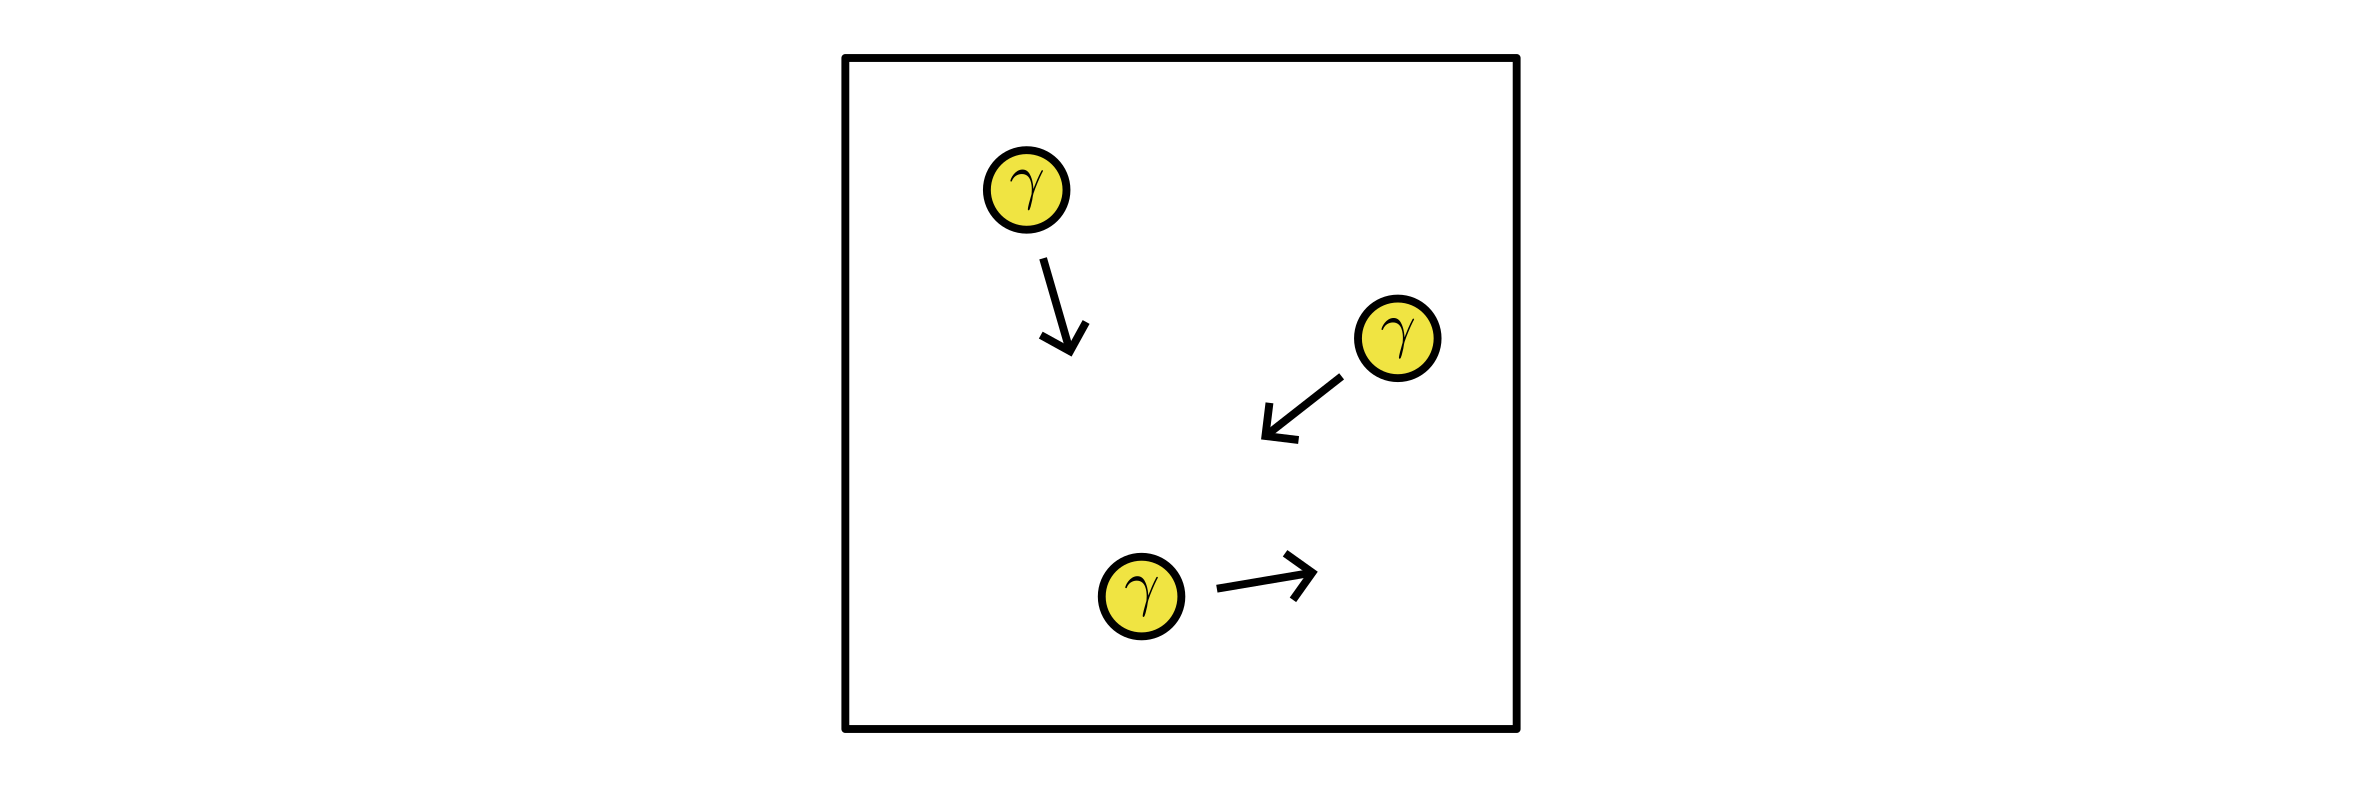
\includegraphics[width=\textwidth]{Figure 9.4.D}
\caption{A random walk from sampled photons must be unbiased from the observer's perspective, and any bias would appear unbiased as the observer drifts}
\end{figure} \noindent
Just as in physics, the speed of light is the same for all observers. Notice how this Gaussian random walk from sampled photons for $\delta t = 1$ and $t^* = 1$ must necessarily have expectation $0$ and variance $c^2$. If it didn't, then photons would be biased in orientation and would not be traveling at the speed of light. Remember, the speed of light is the same for all observers: perceiving non-zero information drift within the system is impossible because observing beings would \textit{drift along} with this \textit{bias in the speed of light}.

Why is this thought experiment important? If an object truly has identical and exchangeable copies of itself one time step into the future, then we consider an object to be fast if it has high velocity variance or slow if it has low velocity variance with respect to applied forces. That means that the eigenclass $G_{\varnothing}$ corresponding to shift distribution:
$$X \sim \textnormal{Normal}(0, \sigma^2)$$
has an average ``stubbornness'' or mass of $m = \sigma^{-2}$. Recall Einstein's famous formula:
$$E = m c^2 \iff c^2 = \frac{E}{m} \iff c^{-2} = \frac{m}{E} \iff m = \frac{E}{c^2}$$
If we assume energy $E$ in our eigenclass $G_{\varnothing}$ to be roughly constant, then we can state that:
$$E = \sigma^{-2} c^2 $$
Unfortunately, defining energy for a Boolean random walk is not so simple. We discuss the issue of definition in detail in \textit{\S 9.5 Issues in Defining Energy}.


This digression about energy gives us justification to understand what an eigenclass $G_{\varnothing}$ is: some rough idea of a local energy minimum of states. We can obtain a sample eigenclass in the following way:
\begin{enumerate}
\item Randomly initialize using some $G_0$
\item Sample $\partial G$ to apply for each $g$ in our sample $G_{\varnothing}$
\item Advance one time step into the future using transition function $f: X_{t} \rightarrow X_{t+1}$
\item Sample some random $G$ using the shift distribution
\item Sampled shifted $g \in G_{t+1}$ form our new samples for $G_{\varnothing}$
\end{enumerate}
We iterate steps $2$ through $5$ as desired. Remember that the shape of our boundary and its sampled boundary distribution may dramatically affect the resulting sample eigenclass.


\section{Issues in Defining Energy}
How do we define the analytical energy of a discrete Boolean random walk? Physics fails to gives us a clear and simple definition that is compatible with Boolean random walks if you assume that \textit{particles move}. Physics gives us a valid definition for Boolean random walks if you understand that \textit{cells rotate}.

In signal processing, the \textbf{signal energy}\index{signal energy} $E$ of a time-varying signal $f(t)$ is given by:
$$E = \int\limits_\infty^\infty |f(t)|^2 dt$$
This definition is reasonable for most continuous signals.
\begin{figure}[H]
\centering
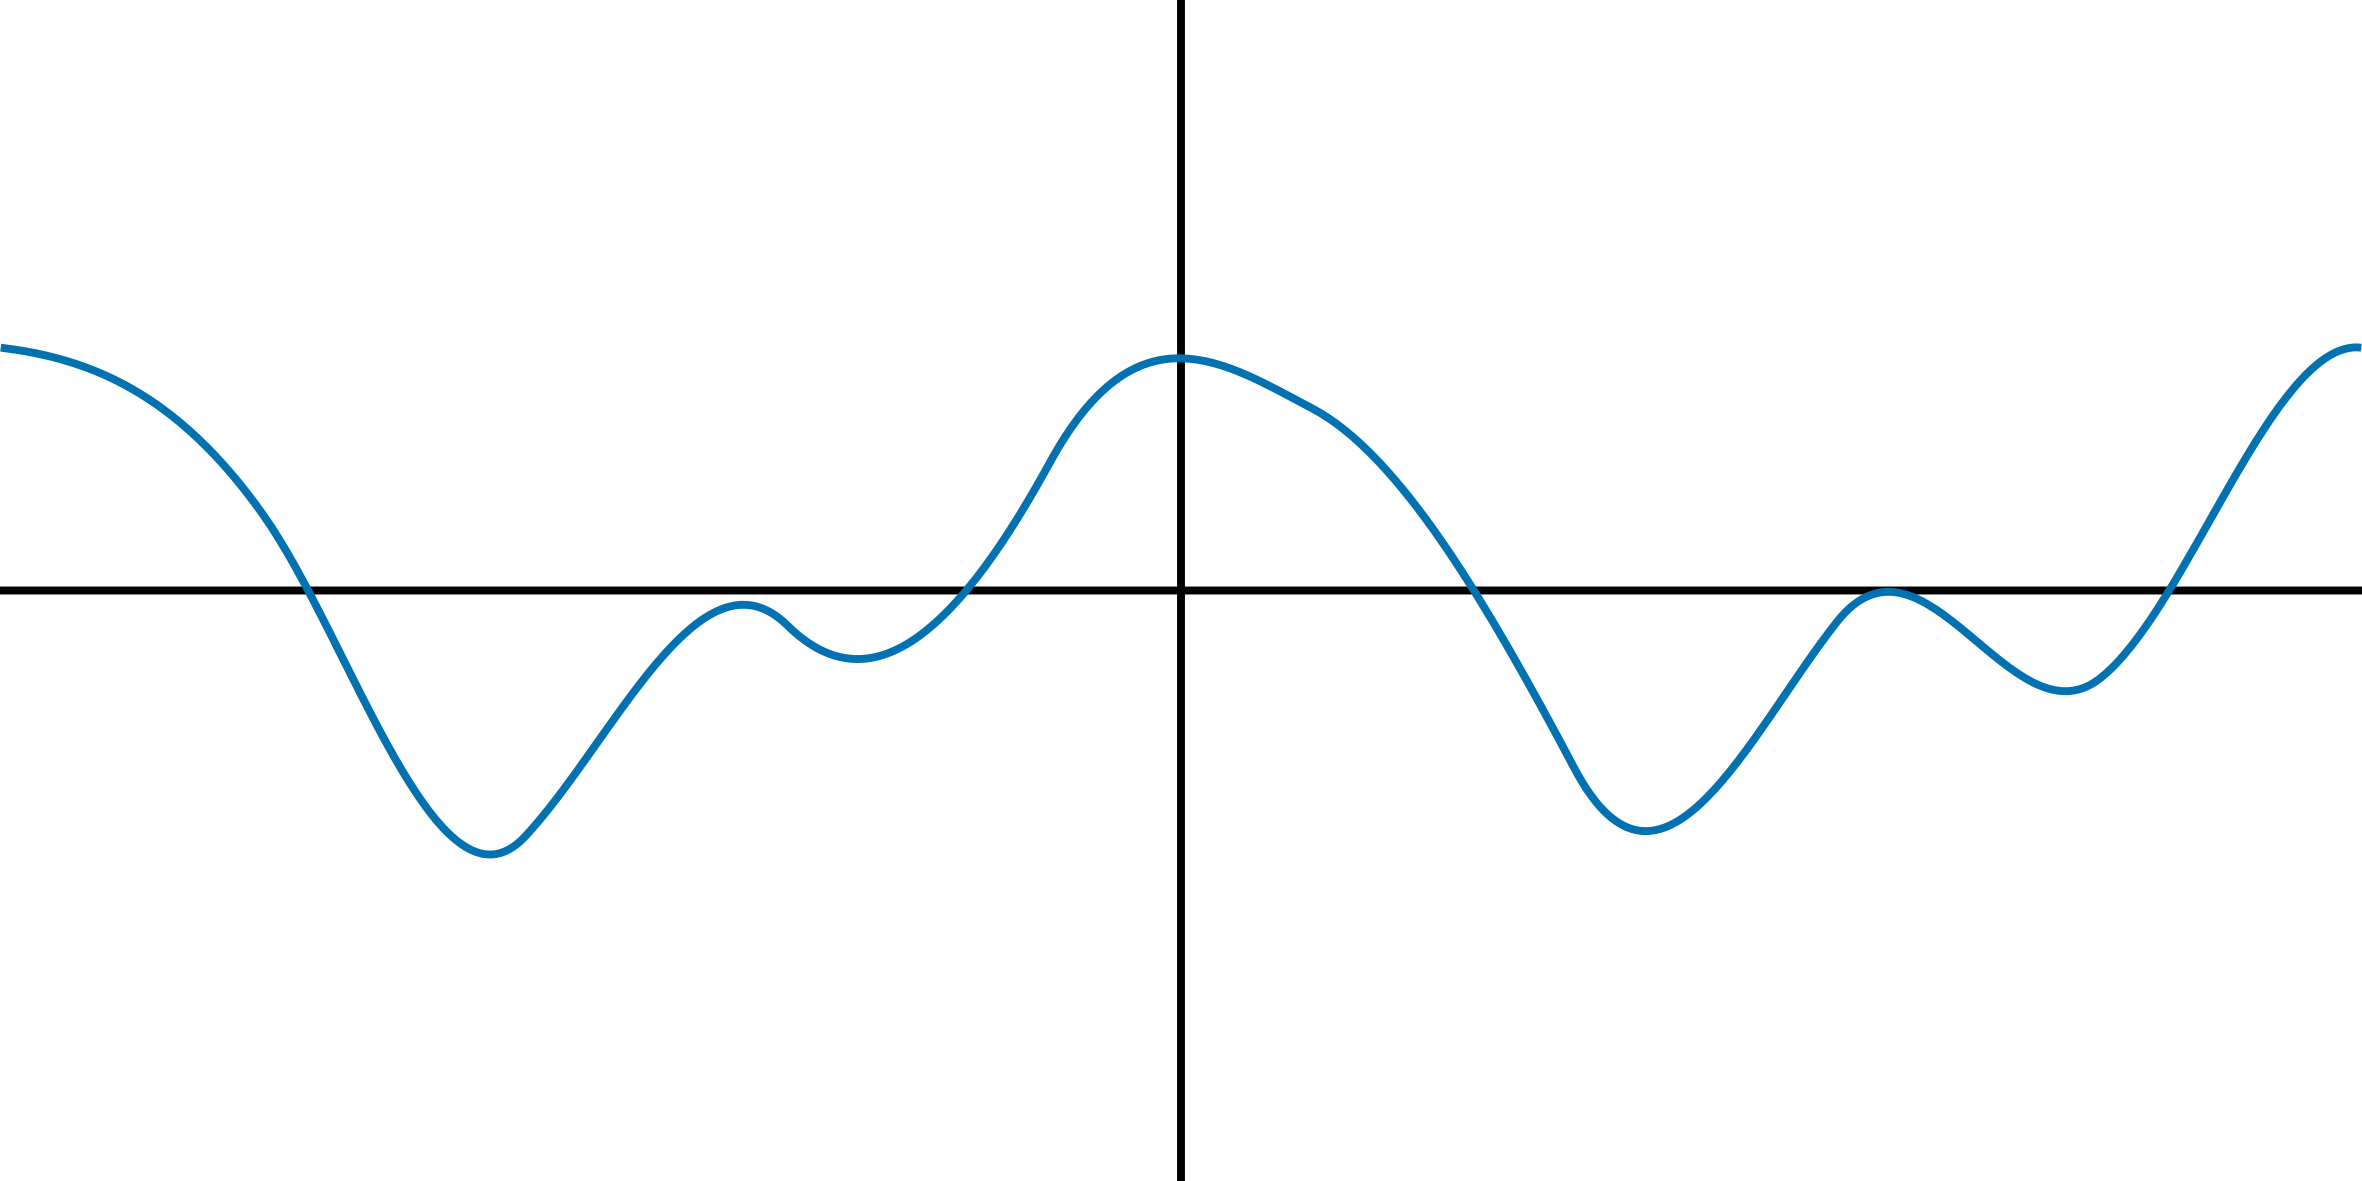
\includegraphics[width=\textwidth]{Figure 9.5.A}
\caption{A continuous signal wave}
\end{figure}
\noindent
This definition works for continuous signal as well as discrete signals:
\begin{figure}[H]
\centering
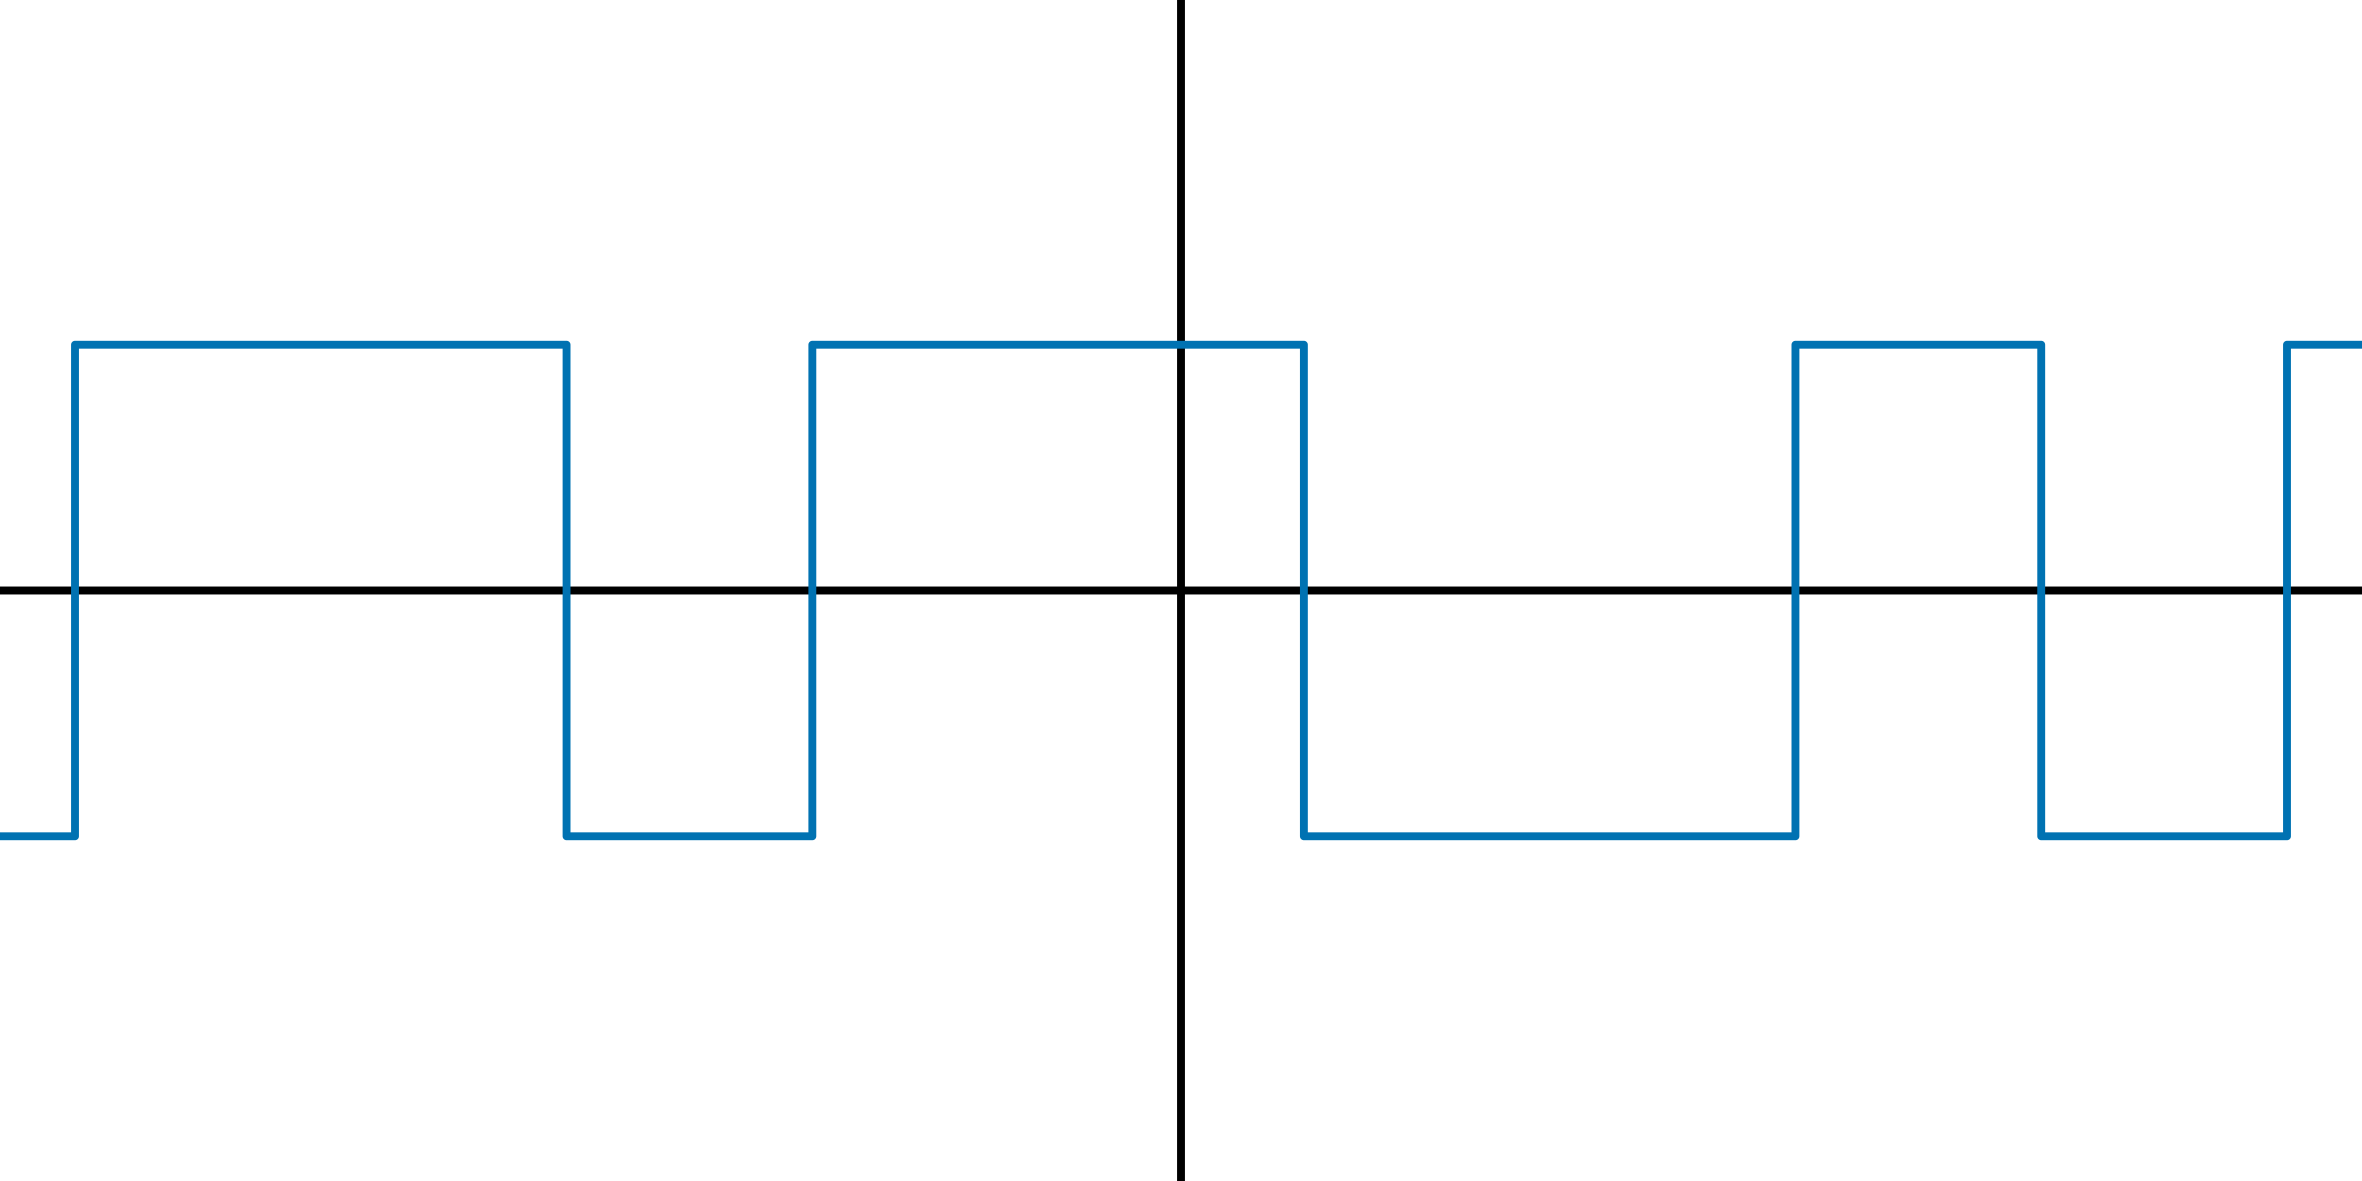
\includegraphics[width=\textwidth]{Figure 9.5.B}
\caption{A digital signal wave representing the value of a Boolean cell in a Boolean random walk}
\end{figure}
\noindent
Any non-decaying signal in the time domain has infinite energy, but we might say that the energy that it outputs over a finite time domain $[0, s]$ is given by:
$$E(s) = \int\limits_0^s |f(t)|^2 dt$$
However, the energy of any finite Boolean signal is proportional to its duration since $|f(t)|^2 = 1$ if $f \in \mathbb B_\pm = \{-1, +1\}$. Therefore, signal energy itself is not informative of the dynamics of a Boolean mechanical system. What is the value in an energy function that does not change value?

In physics, the energy of a system depends entirely on the reference point. The energy in this system does not change at all due to the way that we defined signals in the first place. We can however still measure the \textit{displacement} in the signal between time steps, measuring the \textit{work} by counting how many time the sign of the signal $f$ flipped. Work itself is measure in units of energy. When measuring changes in energy in a discrete system it is more helpful to use discrete versions of continuous formulas to account for abrupt and sharp transitions.

According to the definition of signal energy, the checkerboard harmonic eigenstate $\hat A_2$ would have the same energy as a uniform harmonic eigenstate $\hat A_1$:
\begin{figure}[H]
\centering
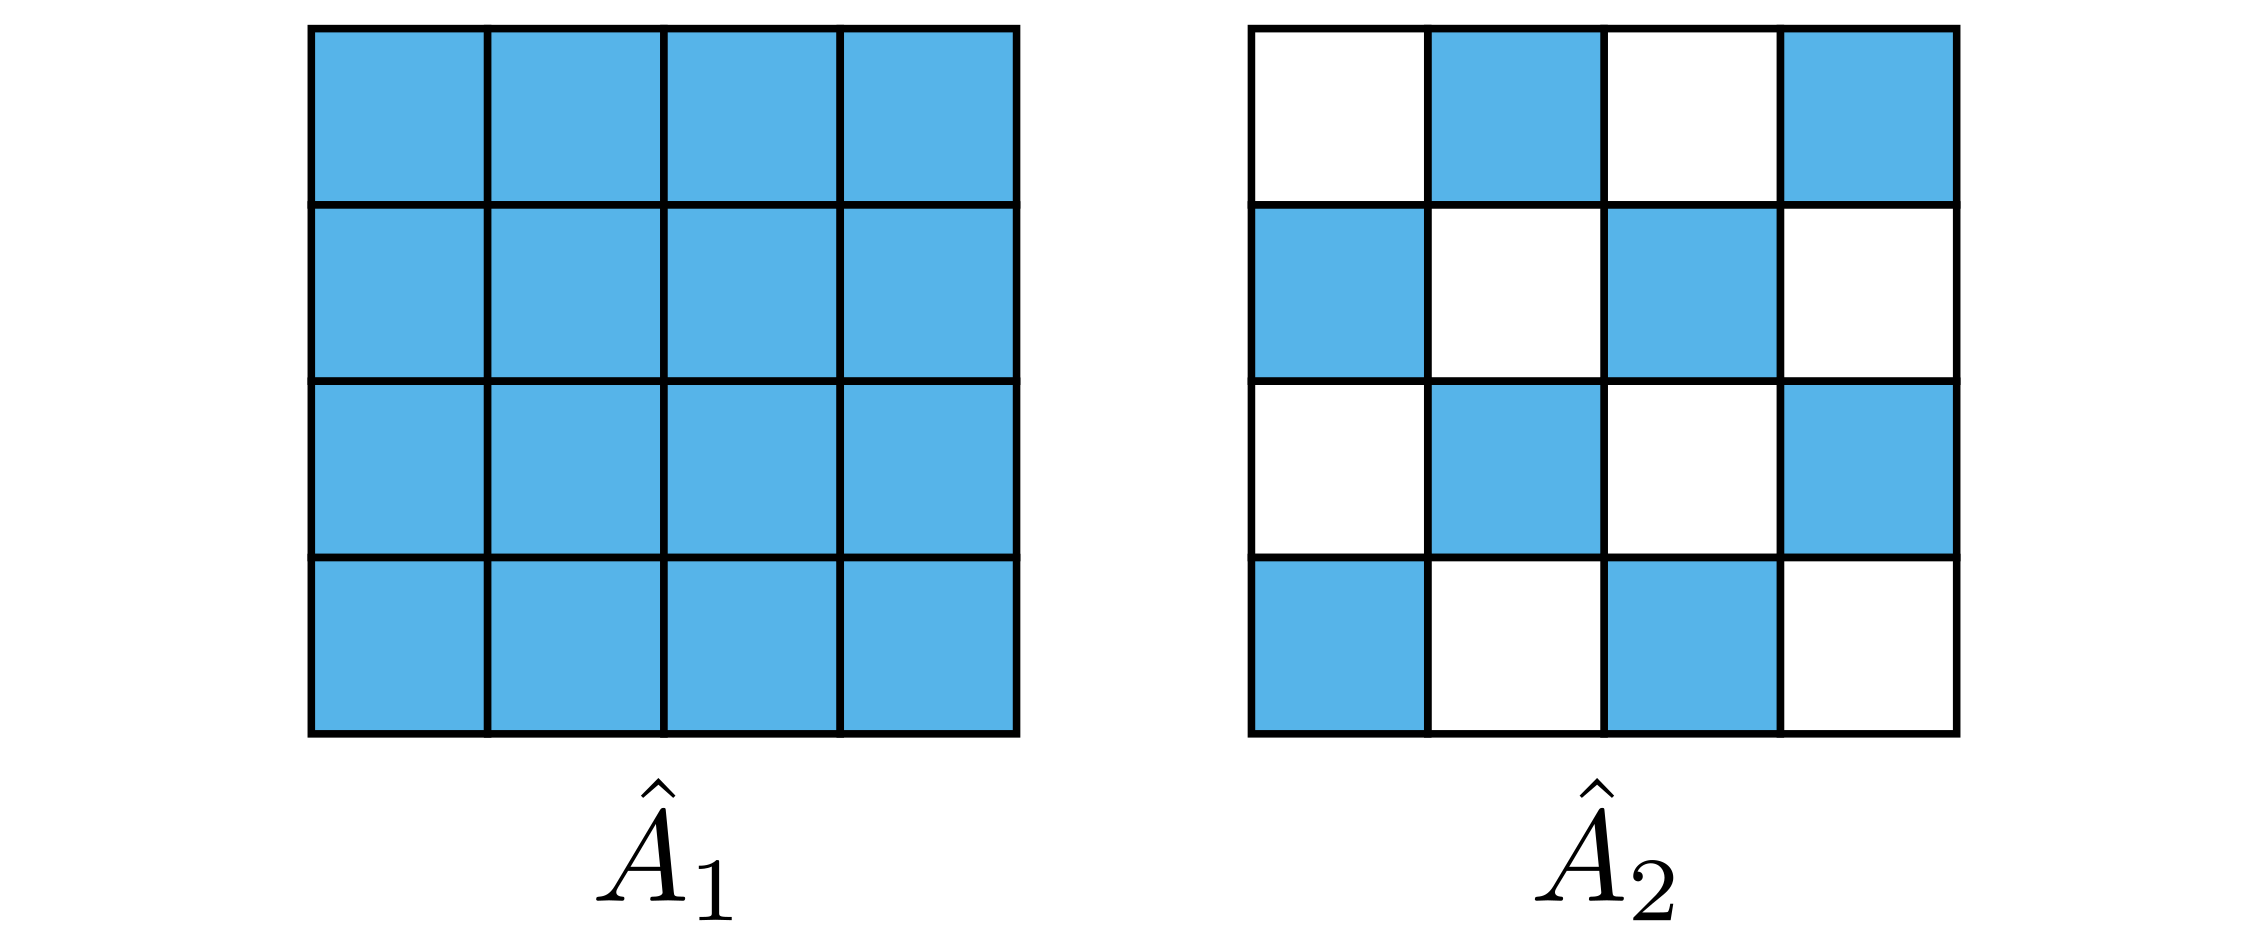
\includegraphics[width=\textwidth]{Figure 9.5.C}
\end{figure} \noindent
Each state takes some work to transition to another state but zero work to transition to itself. Since these normal modes for our signal have eigenvalues of magnitude $\lambda = 1$, these modes have constant energy per cell over both space $x$ and time $t$. However, the other modes with magnitude $\lambda < 1$ will lose energy over time. The eigenvalue is indicative of the spatial relationship between cells, not just the decay of the mode over time.

Recall the $1 \times 5$ bounded simple random walk system. The stochastic matrix $P$ is the following:
$$P = 
\begin{bmatrix}
0 & 1 & 0 & 0 & 0 \\
\frac{1}{2} & 0 & \frac{1}{2} & 0 & 0 \\
0 & \frac{1}{2} & 0 & \frac{1}{2} & 0 \\
0 & 0 & \frac{1}{2} & 0 & \frac{1}{2} \\
0 & 0 & 0 & 1 & 0
\end{bmatrix}
$$
It has an eigendecomposition $P = \Phi \Lambda \Phi^{-1}$ in which:
\[ \Phi = \frac{1}{\sqrt 5}
\begin{bmatrix}
1 & 1 & -1 & -1 & 1 \\
1 & -1 & \frac{1}{\sqrt 2} & -\frac{1}{\sqrt 2} & 0 \\
1 & 1 & 0 & 0 & -1 \\
1 & -1 & -\frac{1}{\sqrt 2} & \frac{1}{\sqrt 2} & 0 \\
1 & 1 & 1 & 1 & 1
\end{bmatrix}\]
\[
\Lambda = \begin{bmatrix}
1 & 0 & 0 & 0 & 0 \\
0 & -1 & 0 & 0 & 0 \\
0 & 0 & -\frac{1}{\sqrt 2} & 0 & 0 \\
0 & 0 & 0 & \frac{1}{\sqrt 2} & 0 \\
0 & 0 & 0 & 0 & 0
\end{bmatrix}
\]
In each representation of the normal mode, the spatial relationship between adjacent cells in space is likewise represented by the eigenvalues. If we have a complex eigenvalue $\lambda$, then we will have a complex eigenvector $\phi$ and a complex valued harmonic eigenstate $\hat A$. 

Let us define the relative sign from Boolean configuration eigenstates $\hat X_i$ to future configuration eigenstate $\hat X_j$ as: 
$$\hat \lambda_{(i,j)} = \frac{\hat X_j}{\hat X_i} = \hat X_j \cdot \hat X_i$$
This convenient property involving the equality of multiplication and division is true due to working with the multiplicative Boolean domain $\mathbb B_\pm =\{-1, +1\}$. Each $\hat \lambda$ may be considered a function upon each cell $x$.

We may then define a symmetric matrix of functions representing the relative sign between two states $\hat X_i$ and $\hat X_j$ like so:
$$\hat \Lambda = 
\begin{bmatrix}
\hat \lambda_{(1,1)} & \cdots & \hat \lambda_{(1,\theta)} \\
\vdots & & \vdots \\
\hat \lambda_{(\theta,1)} & \cdots & \hat \lambda_{(\theta,\theta)}
\end{bmatrix}
$$
A compressed notation is to use $\hat \Lambda = \mathcal X \otimes \mathcal X$. The outer product $\otimes$ of the state space $\mathcal X$ with itself returns the relative sign between every pair of configuration eigenstates.

If we wished to define a matrix using relative half-rotations instead, we will need to use rules involving the logarithm of negative numbers. Knowing that $-1 = e^{\pi i}$ and $i = e^{\pi i / 2}$, we can transfer our domain for each $x$ in $X$ from the Boolean plus-minus domain $\mathbb B_\pm = \{-1, +1\}$ to the Boolean ring domain $\mathbb B_\circ = \{0, 1\}$. We define the relationship between the relative half-rotation matrix $\hat \eta$ and the relative sign matrix $\hat \Lambda$ like so:
$$\hat \lambda_{(i,j)} = e^{\pi i \hat \eta_{(i,j)}}$$
$$\hat \eta_{(i,j)} = \ln(\hat \lambda_{(i,j)}) / (\pi i) = \ln \bigg (\frac{\hat X_j}{\hat X_i} \bigg ) / (\pi i)$$
We may then define the specific Hamiltonian matrix $\hat \eta$ from configuration $\hat X_i$ to configuration $\hat X_j$ like so:
$$\hat \eta = 
\begin{bmatrix}
\hat \eta_{(1,1)} & \cdots & \hat \eta_{(1,\theta)} \\
\vdots & & \vdots \\
\hat \eta_{(\theta,1)} & \cdots & \hat \eta_{(\theta,\theta)}
\end{bmatrix}
$$
Normally, we reserve the symbol $\eta$ for the Hamiltonian energy of a Boolean mechanical system and $\lambda$ for the eigenvalues of a stochastic matrix. The work between two states is given by $\hat \eta$, stated in units of energy.\footnote{An alternative representation is to consider the matrix of full rotations $\hat \sigma$, computed as $\hat \sigma = \hat \eta / 2$. The function $\hat \sigma$ assigns a value to each $x$ from the set $\{0, \frac{1}{2}\}$ such that $\hat \sigma (x)\in \{0, \frac{1}{2}\}$.}

\textbf{Work}\index{work} is the sum of forces along a path, and the field of values for the force is scalar-valued. A force is a \textbf{conservative force} if the work is the same regardless of path taken. This necessarily means the work between a point and itself must equal $0$. We distinguish work from energy because work is the theoretical minimum amount of energy needed to turn one state into another. It is possible to waste energy by ``running in circles'' literally and metaphorically.

In our system, the work needed to rotate a state to itself is zero. The relative half-rotation between a state $\hat X_i$ and itself is given by $\hat \eta_{(i,i)} = 0$. This $\hat \eta$ is itself a field of values upon each cell $x$, and it indicates that a vertex between the aforementioned cell and some neighboring cell was chosen for a maximal independent set $H$. This means that $\hat \eta(x)_{(i,i)} = 0$ for each cell $x$ for all possible indices of $i$. This is because the relative half-rotation for each cell is $0$. 

Allow us to construct an elementary example. A two-step path between two states involves three total states: 
$$\hat X_a \rightarrow \hat X_b \rightarrow \hat X_c$$
If a cell $x$ performs a half-spin from $\hat X_a \rightarrow \hat X_b$, then the value given by $\hat \eta$ is:
$$\hat \eta_{(a,b)} = 1$$
If a cell $x$ performs a half-spin from $\hat X_b \rightarrow \hat X_c$, then the value given by $\hat \eta$ is also:
$$\hat \eta_{(b,c)} = 1$$
If the total number of half-spins in the path for a cell is $1 + 1 = 2$, then the relative half-spin of that cell from $\hat X_a \rightarrow \hat X_c$ is $0$ even though it rotated twice in the path. If $\mathcal S$ is the (natural) number of half-rotations of a path, then:
$$\hat \eta = \mathcal S \ (\textnormal{mod} \ 2)$$
Notice that this means that $0 = \mathcal S \ (\textnormal{mod} \ 2)$ if $\mathcal S$ is some even non-negative integer and $1 = \mathcal S \ (\textnormal{mod} \ 2)$ if $\mathcal S$ is some odd non-negative integer. We assume that energy is measured unless between two integer time steps, and we assume that it we cannot measure work at smaller time steps.

We call the sum of work the \textbf{action}\index{action} $\mathcal S$, and it counts the number of half-rotations for each cell $x$ as given by the time integral:
$$\mathcal S(x, s) = \sum\limits_{t=0}^s \eta(x, t)$$
in which $\eta(x, t)$ counts whether a cell $x$ experiences a rotation or not from time $t$ to $t+1$. Again, we count if a cell rotated or not using the Boolean ring domain, $\eta(x, t) \in \{0, 1\}$.

In physics, \textbf{work} is calculated in units of \textit{energy}. Work has a dimensionality of $\frac{m l^2}{t^2}$, or mass times length squared divided by time squared. The time integral of work or \textbf{action} in units of \textit{angular momentum} with a dimensionality of $\frac{m l^2}{t}$. If we take a sample path and add up all our individual works to obtain the action $\mathcal S$, we should get the angular momentum of the path precisely in units of $\hbar$.

To make this more visual, let us return to our $2 \times 2$ oscillator example for a Boolean random walk:
\begin{figure}[H]
\centering
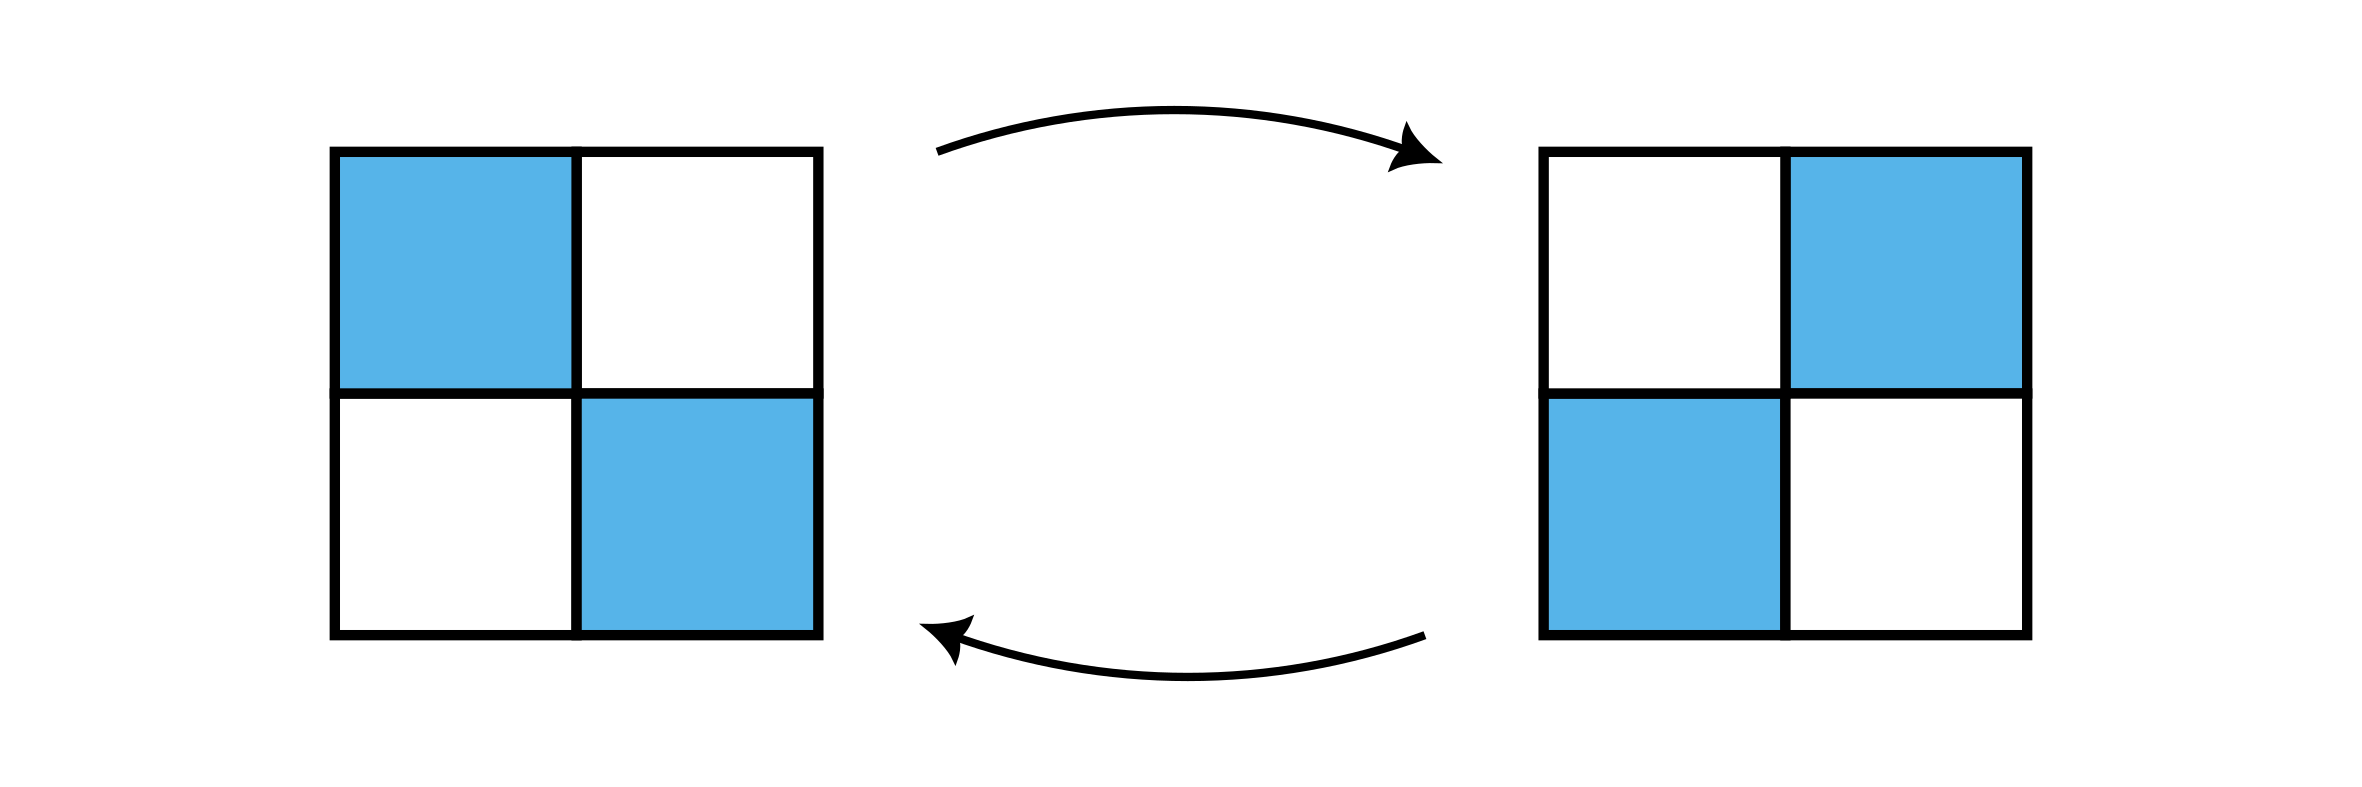
\includegraphics[width=\textwidth]{Figure 9.5.D}
\end{figure} \noindent
After $1$ time step, the action is precisely $\mathcal S(x, s) = 1$ for each cell. After $2$ time steps, the action is precisely $\mathcal S(x, s) = 2$ for each cell. 

If $\mathcal S(x, s)$ is odd, then the cell $x$ must have a net rotation of $1 \pi i$. If $\mathcal S(x, s)$ is even, then the cell must have a net rotation of $2 \ (\textnormal{mod} \ 2) = 0$. We then say that $\mathcal S(x, s) \hbar$ is action of the cell after $s$ time steps, stated in units of angular momentum. In this deterministic system, the work experienced is precisely $\mathcal S(x, s) \hbar$ after $s$ time steps since initial time $t=0$.

It would like to point out that in physics, the action between the starting state and ending state is not measurable. In Boolean statistical mechanics, we may cheat and find the action of a specific path or at least the action between two states. If you are only given two states in Boolean statistical mechanics, it is not possible to determine the exact path of states taken or the time taken between them. If you were to augment a specific system with some measurement function, then the \textit{reliability} of measurement function within the system itself would be questionable.

In physics, the work $W$ is equal to the change in the kinetic energy $T$ such that $W = \Delta T$. A potential function $V$ is conservative such that $W = -\Delta V$. Calculating the work of a Boolean random walk using the physics definition would require summing the differences along faces for each cell, in essence counting the number of vertices in the finite-difference mesh $T$. This is different from the way that we calculated it since we were only calculating the rotation of a cell/hyperedge. In a struggle for a proper definition of energy, we have instead needed to properly redefine work and action from first principles.


\chapter{Macroscopic Behavior}
\section{Motivations for Macroscopic Behavior}
What are large scale patterns are we looking for in Boolean statistical mechanics? What large scale patterns are we looking for in Boolean random walks? It can be hard to parse out when we are looking at the reverie of pixels dance in a way that is foreign to us. Why might formal analysis in the usual way be insufficient?

Even relatively small Boolean random walks require impossibly large amounts of computing power and memory in order to represent their Markov process as a stochastic matrix. A reflecting system $X_t$ with $k$ particles and $(N-k)$ antiparticles has an adjacency matrix $A_{\theta \times \theta}$ in which $\theta = {N \choose k}$, far outpacing the number of electrons in the universe that could be used to represent it for a humble $20 \times 20$ system with $\theta = {{20 \times 20}\choose{20 \times 20 \div 2}}$ possible states. Obtaining the stochastic matrix $P$ by applying a measure to $A$ to finite precision would take even more computing power. 

This makes it necessary to create a description or heuristic of emergent behavior at large scales, or macroscopic behavior. Each microstate $g$ in a macroparticle class $G$ must have some unique properties regarding its eigenvalues that allow it to reliably permute into some other $g \in G$ while in a stochastic vacuum.

All macroparticles posit interior randomness and exterior randomness. The interior randomness of a macroparticle represents truly fluctuating information states that are strictly unresolved unless accessed in a specific way. The exterior randomness of a macroparticle represents ignorance of some non-fluctuating or low entropy change in the information state, resulting in perceived randomness. For example, two macroparticles may have truly random momenta distribution (interior) at any given time step but have linked memories that we are ignorant about, such as one being spin up and the other being spin down, until a physical object measures them (exterior). 

If they have a Bernoulli distribution for spin (up or down) that is correlated, then it should decay approximately geometrically or exponentially with time. For any physical system whose normal modes can be approximated using Boolean mechanics, we should expect exponential decay to underlie all interactions. Correlation and its decay between two points in space and time is not magic but a natural consequence of normal modes. I doubt this boring and rigorous interpretation will reduce how often popular science uses the word ``quantum'' in every headline to garner attention.


\section{Ergodic Construction Theorem}
For an ergodic Boolean mechanical system of infinite size, random spatial sampling is ergodic. This is only true with the following properties:
\begin{quote}
0. $x \in \mathbb B$: Each cell $x$ is Boolean

1. $X = (x_1,...,x_N)$: The cells composed the system $X$ (in a partial cube in $d$-dimensions)

2. $\mathcal X = (X_1,...,X_\theta)$: The state space $\mathcal X$ is all possible Boolean configurations of $X$

3. $\exists x_i \in \gamma(x_j)\forall i, j$: Each cell is a neighbor of another cell

4. $f: \mathcal X \rightarrow \mathcal X$: The transition function $f$ maps possible system states to otthers in the state space

5. $\underbrace{f \circ ... \circ f}_{{t \ \textnormal{times}}}(x) = f(x, t)$: The time variable $t$ represents composing the function $t$ times

6. $f(x_i) f(x_j) \neq f(x_i, x_j) \iff x_i \in \gamma(x_j)$: Cells are not independent 
(with respect to time if they are neighbors

7. $f(X, t) \cong f(e^{\frac{\partial}{\partial x} z}X, t), \ z \in \mathbb Z^d$: The transition function is isomorphic under translations in space in $d$-dimenions

8. $f(X,t) = P^t$, $P$ is an ergodic transition matrix
\end{quote}
These rules are important because we need some almost sure guarantee that a random system can arbitrarily execute any random function.\footnote{A Boolean random walk, the often used example, fails this ruling because there is no way to introduce changes to the number of particles and antiparticles. However, it is an excellent study of Boolean statistical mechanics in general.}

The \textbf{infinite monkey theorem}\index{infinite monkey theorem} states that a uniformly random sequence of letters from an alphabet $A$ of length $n$ will \textit{almost surely} produce any specific text as $n \rightarrow \infty$:
\begin{figure}[H]
\centering
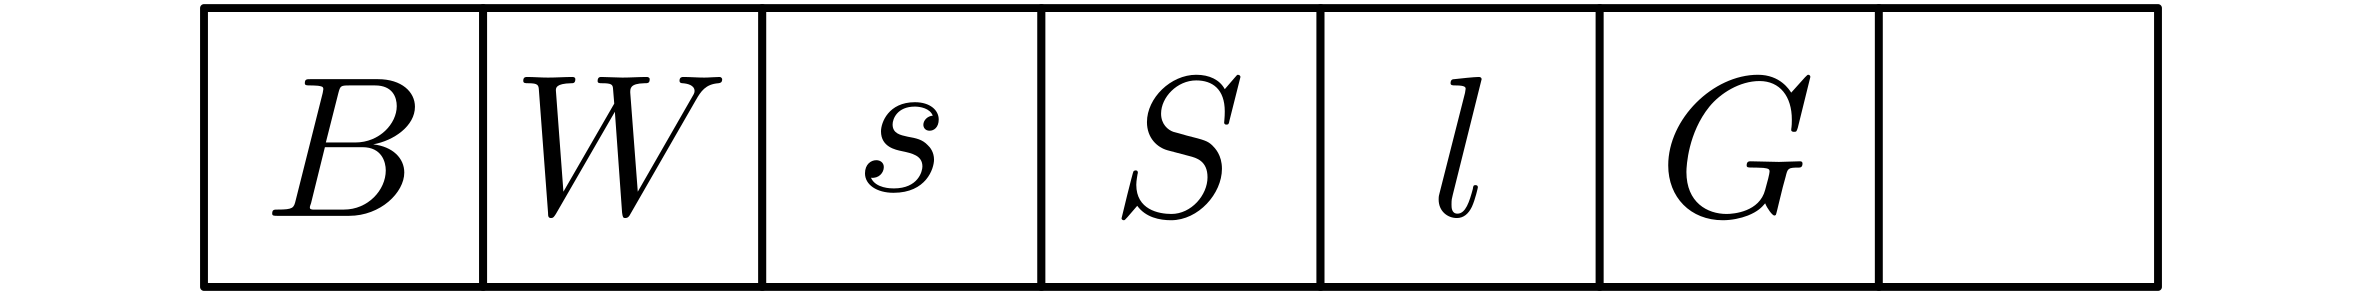
\includegraphics[width=\textwidth]{Figure 10.2.A}
\caption{A infinite random sequence of letters will contain every known combination}
\end{figure} \noindent
For example, a monkey randomly pressing keys will eventually produce the written works of Shakespeare if given infinite time because Shakespeare's works would be is a finite subsequence of an infinite random sequence. This theorem is important because we are extending this theorem to randomly sampling an infinite lattice, equivalent to randomly sampling from some undefined probability distribution. Even if our transition function has heavy spatial dependence, sampling from an infinite space allows us to assume uniformity.\footnote{Technically speaking, there is no finite algorithm to uniformly sample from an infinite set. Such is an improper prior distribution.}

By generalizing the infinite monkey theorem to a Boolean transition function, we can assume that an infinite-sized and infinite-time ergodic computer must be able execute every finitely computable function. It does this by arranging small, simple parts into large, complex wholes. The infinite monkey theorem may derived from the \index{second Borel-Cantelli lemma}\textbf{second Borel-Cantelli lemma} which states that if the probability sum :
$$\sum\limits^\infty_{n=1}P(X_n) = \infty$$ 
for independent events $(X_n)^\infty_{n=1}$, then the probability that $X$ occurs infinitely many times is $1$.\footnote{This has no bearing on the local ratio of events. By definition, each left half of a macroparticle that is adjacent to its other right half has twice the frequency of the original macroparticle.} As long as our construction has an entropy rate beneath \textbf{Shannon's limit}\index{Shannon's limit} given by the \textbf{noisy-channel coding theorem}\index{noisy-channel coding theorem}, we can guarantee that the probability of error in our macroparticle is arbitrarily small. 

The \textbf{ergodic construction theorem}\index{ergodic construction theorem} of Boolean mechanics dictates that uniform sampling of $d$-dimensional cubic systems size $N$ from an infinite Boolean mechanical system $X_\omega$ should obey Binomial distribution for a target state in which $p$ is the asymptotic probability of the target configuration in the universe. Likewise, it obeys the geometric distribution for the number of samples acquired until the first successful sample of the desired state. It also obeys the negative Binomial distribution for the $r$-th successful sample. 

This means that it is statistically inevitable that an infinite-time, infinite-space Boolean mechanical system will produce a complex network of simpler systems with specific behaviors such as attraction versus repulsion or replication versus annihilation. No matter how rare the specific behavior or arrangement, any finite Boolean configuration with non-zero probability eventually occurs. This includes the stable and long-lasting structures that we refer to as particles. By sampling from an infinite space uniformly, we are ignoring the assumption of spatial correlation of adjacently sampled blocks.

The specific systems that we are interested in are called ``macroparticles'', and we assume that they have the following properties:
\begin{enumerate}
\item Stochastically resonant with respect to background noise, or is roughly a harmonic function with respect to time and space in some noisy medium.
\item Radially symmetric logical functions that send information and receives information, or is itself a self-stable information carrier.
\item Created when certain subsets of structured information is encrypted and is annihilated when decrypted by perfect or partial decryption.
\end{enumerate}
The first condition is the most important as it asserts the stability of a system with respect to time and space. The second condition is more of a matter of convenience and technically incorrect: Not all harmonic functions are necessarily radially symmetric. In \textit{\S 8.5 Partial Differential Equation}, a harmonic function is necessarily restricted to some boundary. We should say that the boundary of the harmonic function is necessarily finite or may be enclosed in some sphere. The third condition is something of a consequence of trying to find a \textit{stable construction}: it must resist changing under most configurations.

\section{Stable Contruction Hypothesis}
This is an extension of the ergodic construction theorem of the previous section. The \textbf{stable construction hypothesis}\index{stable construction hypothesis} states that it is possible to create arbitrary constructions of eigenclasses $G_\varnothing$, and this arrangement behaves somewhat predictably under randomly initialized vacuum noise. If we are looking for something to call a macroparticle, then it must be stable under some noisy conditions.

A macroparticle defined by an \textbf{eigenclass}\index{eigenclass} is a subset of states that rows in a transition matrix $P$ are collinear after some finite time. It appears as a set of substates that tend to cycle among themselves. These correlated states have patterns that are translated within each other, creating the illusion of movement. Recall a Boolean mechanical system with stochastic matrix $P$ has an eigenvalue $\lambda_i = \mu_i e^{\omega_i}$ with an absolute magnitude of $\mu_k$ and a frequency of $\omega_i$. The period $\omega_i^{-1}$ implies that some pattern repeats after that period of time. 

The word ``class'' in eigenclass is twofold. It is used in the Markov communication class sense: over short time periods, any individual pattern tends to reproduce patterns in the same class due to the way it diffuses in the state space. It is also used in the statistical classification sense: The rows of $P^t$ can be classified using a modified $k$-means clustering algorithm to represent similar future distribution. The word ``eigen'' in eigenclass is related to the idea of how eigenvalues dictate flow rates between states in a transition matrix. For more details, see \textit{\S Appendix D: Class Stochastic Matrices}.

It is important that higher-order arrangements of eigenclasses behave identically under interchange of any particular class state with another class state. From there, it is possible to represents arbitrary functions such as some abstract macroscopic representation of \textbf{AND}, \textbf{OR}, or \textbf{NOT} Boolean functions. This does not mean that all complex constructions are necessarily stable after the computation has completed, but it does mean that stable structures can be found, can be created by other structures, and can interface with other structures to represent some function.

Finding a large eigenclass for some desired surface or transition rule can be restrictive and time-consuming. It should be possible to create a larger particle using some function of smaller particles that interact with each other and stay close to one another. An eigenclass composed of three smaller eigenclasses orbiting around each other is entirely possible, but it is perhaps not so simple to observe the phenomenon's existence or stability with the computational power currently available. The three-body problem of celestial objects already behaves chaotically due to sensitivity to initial conditions. Even with this in mind, it is fair to assume that three copies of an object that we define as stable (not dissociating in vacuum noise) are unlikely to decay if placed a reasonable distance apart.

The ergodic construction theorem is important because it directly implies the existence of logic gates and finite Turing machines constructed using arrangements of these macroparticle eigenclasses. Even though the Boolean functions created would be probabilistic, the perpetual and stable existence of such macroparticles means the function's output is low variance in some abstract space, as opposed to the direct space of representation via Boolean values. Quantum circuit diagrams are the current tool used to describe probabilistic logical functions in physics classes.

This implies and is implied by the fact that you need specific constructions of Boolean values to encrypt and decrypt Boolean harmonic eigenclass, likewise called matter in physics. In the same way that biological organisms cannot freely transform materials outside of their domain of molecular control, it is not possible to have a general purpose machine that identifies \textit{any} macroparticle arrangement and deconstructs into smaller constituent eigenclass plus free energy. That is because it would be mathematically equivalent to solving the \textbf{halting problem}\index{halting problem} with a finite machine. We discuss the halting problem in \textit{\S 6.7 Stochastic Turing Systems}.

In general, Boolean satisfiability is \textbf{NP}-complete. The \textbf{Boolean satisfiability}\index{Boolean satisfiability} problem asks if there is some combination of $n$ Boolean inputs that produces a single true Boolean output. The simplest being the 3-SAT problem, $f: \mathbb B^3 \rightarrow \mathbb B$:
$$\underset{x_1,...,x_3}{\textnormal{argmax}} \ f(x_1,...,x_3)$$
It is therefore likewise at least \textbf{NP}-complete to check if a function accepting some Boolean $n$-input function will create some target Boolean $m$-output. We shall call the Boolean input $I$ that produces the desired Boolean output $O^*$ as $I^*$:
$$I^* = \underset{I \in \mathbb B^n}{\textnormal{argmax}} \Big( f(I) \leftrightarrow O^* \Big)$$
Note that we are abusing notation by referring to the total/group biconditional operator $\leftrightarrow$ for multivariable Boolean:
$$(f(I) \leftrightarrow O^*) = 1 \cdot \prod\limits_{i=1}^n (\leftrightarrow (o_i \leftrightarrow o_i^*))$$
We generalize this idea to multiple desired outputs for the purpose of finding some eigenclass. If we are relating this to any real theory of physics, then finding some input that maximizes the output is generally \textbf{NP}-complete. Since physics is not error-free, we need other forms of computational complexity as defined in \textit{\S 6.8 Computational Complexity}.

A general purpose matter decryption machine in Boolean statistical mechanics would need to be able to solve the halting problem for Turing machines for the following reasons:
\begin{enumerate}
\item The encrypted space $S$ evolves with its surrounding environment according to some probabilistic Boolean function. It may be of any size $|S|$ that our decryption machine is ignorant about.
\item The general purpose decryption machine $M$ must construct a region about $S$ that will produces the set of target states $O^*$, therefore it must find some $I^*$ even before it has probed the construct $S$.
\item Probing the construct $S$ must not change it in any meaningful way.
\item The finite algorithm $I^*$ that $M$ executes must therefore know all possible future distributions of the interaction between $S$ and $I$ that will produce $O^*$, for example states of released energy in physics.
\item The finite machine $M$ must have more entropy that the Boolean state space of $S \cup I$ in order to represent more information states.
\item The finite machine $M$ must adapt to the unknown cardinality of the encrypted space $S$, even though measurements of $S$ directly transform it.
\item The decryption machine $M$ must be capable of decrypting itself as an input for $S$.
\end{enumerate}
This poses a lot of physical and mathematical contradictions. There are perhaps two exceptions: empty space and black holes.

The \textbf{pure infection algorithm}\index{pure infection algorithm} defined in \textit{\S 6.7 Stochastic Turing Systems} is perhaps the closest thing to something that generates empty space. What might be considered a space-eater bomb would soon become empty space if it were to successfully infect all of free space. This is because a space-eater bomb became the majority, thus empty space.

The other possibility involves black holes, or the equivalent in Boolean mechanics being black eigenclasses. Instead of having a large target state space that it needs to represent, its converts relatively small objects into copies of itself and expands its radius. This is not the same as decrypting matter into freely usable energy since the matter is absorbed. If you pay attention to this interpretation, it means that black holes do not convert vacuum fluctuations of empty space into more black hole mass.\footnote{Though a black hole does not convert \textit{on average}, it still may fluctuate due to spontaneous excesses and deficiencies in energy.} Considering these similarities, it is possible that a black hole is actually hollow and instead is a shell that behaves as having the properties of mass. A more deranged interpretation is that empty space has local bias in its angular momentum, and black holes have opposing angular momentum to its local vacuum. 

This framework would imply that the surface of a black hole is necessarily diamagnetic, commonly known as non-magnetic, due to opposing the spin-field of the vacuum. Since black holes only have properties of mass, charge, and angular momentum, it makes sense to assume that a black hole forms due to the exclusion principle preventing $\frac{1}{2}$-spin particles from occupying the same quantum state, particularly angular momentum. It is unclear if this necessarily means that the interior black hole has the same global bias in angular momentum that opposes the global bias in angular momentum of the vacuum or if it is strictly local.

As a closing statement, no organism of finite size may bend the universe to its will. It may at most observe what the universe is capable of and imitate it or construct machines with restricted ability to transform other objects. One may not overwrite reality from within without playing by its rules. No gods, so to speak.

\section{Poisson Process for Rare Gates}
A relatively rare set of Boolean structures that behave like probabilistic logic gates is approximately distributed in space according to the Poisson distribution. The occurrence or detection of these logic gates $G$ per unit of volume in a sequence is thus described by a Poisson process. A \textbf{Poisson process}\index{Poisson process} is often used to describe distributions of discrete arrivals in continuous time or space, but sufficiently rare sets of logic gates $G$ may be approximated as ``arriving'' probabilistically in discrete amounts. The rarity of their occurrence per unit of space justifies a continuous approximation, such as galaxies.

Suppose that we idealize adjacent chunks of space as being spatially uncorrelated in structure.\footnote{This is not true of fluid simulations in general, neither is it true of the distribution of galaxies due to clustering.} If the probability that a cubic chunk of space with volume $V$ contains an element from $G$ is given by probability $p$, then repeated expansions of this cubic chunk may consider the arrival of elements of $G$ as arriving according to the Poisson distribution:
$$G \sim \textnormal{Poisson}(\lambda = \frac{p}{V}, t = V)$$
in which $V$ is the total volume of the cubic chunk. Successive cubic chunks of space is less ideal for defining a Poisson process in Boolean mechanics because of the way that logic gates may appear between the boundary of consecutive cubic chunks.


\section{Spatially Crystallizing Logic Gates}
A system that is in a supersaturated information state may crystallize into an ordered, low entropy permutation spontaneously. In exchange, the crystallized system expels the leftover energy into its surrounding environment. The newborn crystal lattice will grow into adjacent spaces so long as they are relatively oversaturated, and the process may be initiated by a catalyst such as a seed crystal. What happens if we take this knowledge and generalize it to Boolean statistical mechanics?

Under the perspective of Boolean mechanics, the Big Bang is a crystallization process of space that is supersaturated like a black hole. This crystallized space is specifically the vacuum, a permissible space that permutes objects with copies of itself if these objects have special properties. This is an incomplete view tainted by physical intuition. What truly happens is that the permissible space lattice applies a mutual transformation to itself and the object, and the object that continually transforms is an eigenfunction of the lattice. Example eigenfunctions are precisely the lattice itself or the large-scale patterns that we perceive as macroparticles.

The expulsion of excess energy from newly crystallized logic gates is the reason the the extreme temperatures of the Big Bang. If free energy is dissociated matter while matter is associated free energy, then the high entropy free energy must associate into higher-order structures to be stable eigenfunctions of the lattice. This crystallization process need not be perfectly geometric or simple. Recursive processes of fractal dimension rarely produce perfect crystals in nature due to the probabilistic nature of particles in quantum mechanics.

The crystals that define empty space may also be chiral such as a sugar molecule, which may be left-handed or right-handed. Our bodies cannot recognize and process left chirality sugar. We shall refer to our observable universe's permissible space as right aether if it happens to be chiral, although it unreasonable to assume that there is a right-handed bias in the vacuum without physical evidence. There would be unknown consequences to chirality in communicable space in a 3D Boolean random walk system, but even small biases may change what macroparticles are preferred or even allowed. It is likely that any 3D Boolean mechanical system will have skewness in its 3 dimensions, but the skewness of a 3D Boolean random walk will persist due to locally restricted movement.\footnote{Skewness of a random variable $X$ is defined as $\mathrm{E}[(\frac{X-\mu}{\sigma})^3]$.}

The idea that the heat released from the Big Bang is the result of the crystallization of communicable space is speculative at best. The best case scenario is that a de facto \textbf{Seed of Logos}\index{Seed of Logos}, the seed crystal permutation that catalyzed the creation of the universe, is found for a finite 3D Boolean mechanical system simulation. It may not be Boolean random walks specifically. Testing top-down for the ``correct'' rules of Boolean mechanics exactly is physically impossible while simulating bottom-up the emergence of a whole universe is computationally impossible. Any measure-preserving stochastic Turing system that will compute every computable function non-uniformly is a viable candidate for simulating our universe.

\section{Resimulation Size and Time}
Conway's Life is a cellular automaton that is capable of simulating itself at larger scales:
\begin{figure}[H]
\centering
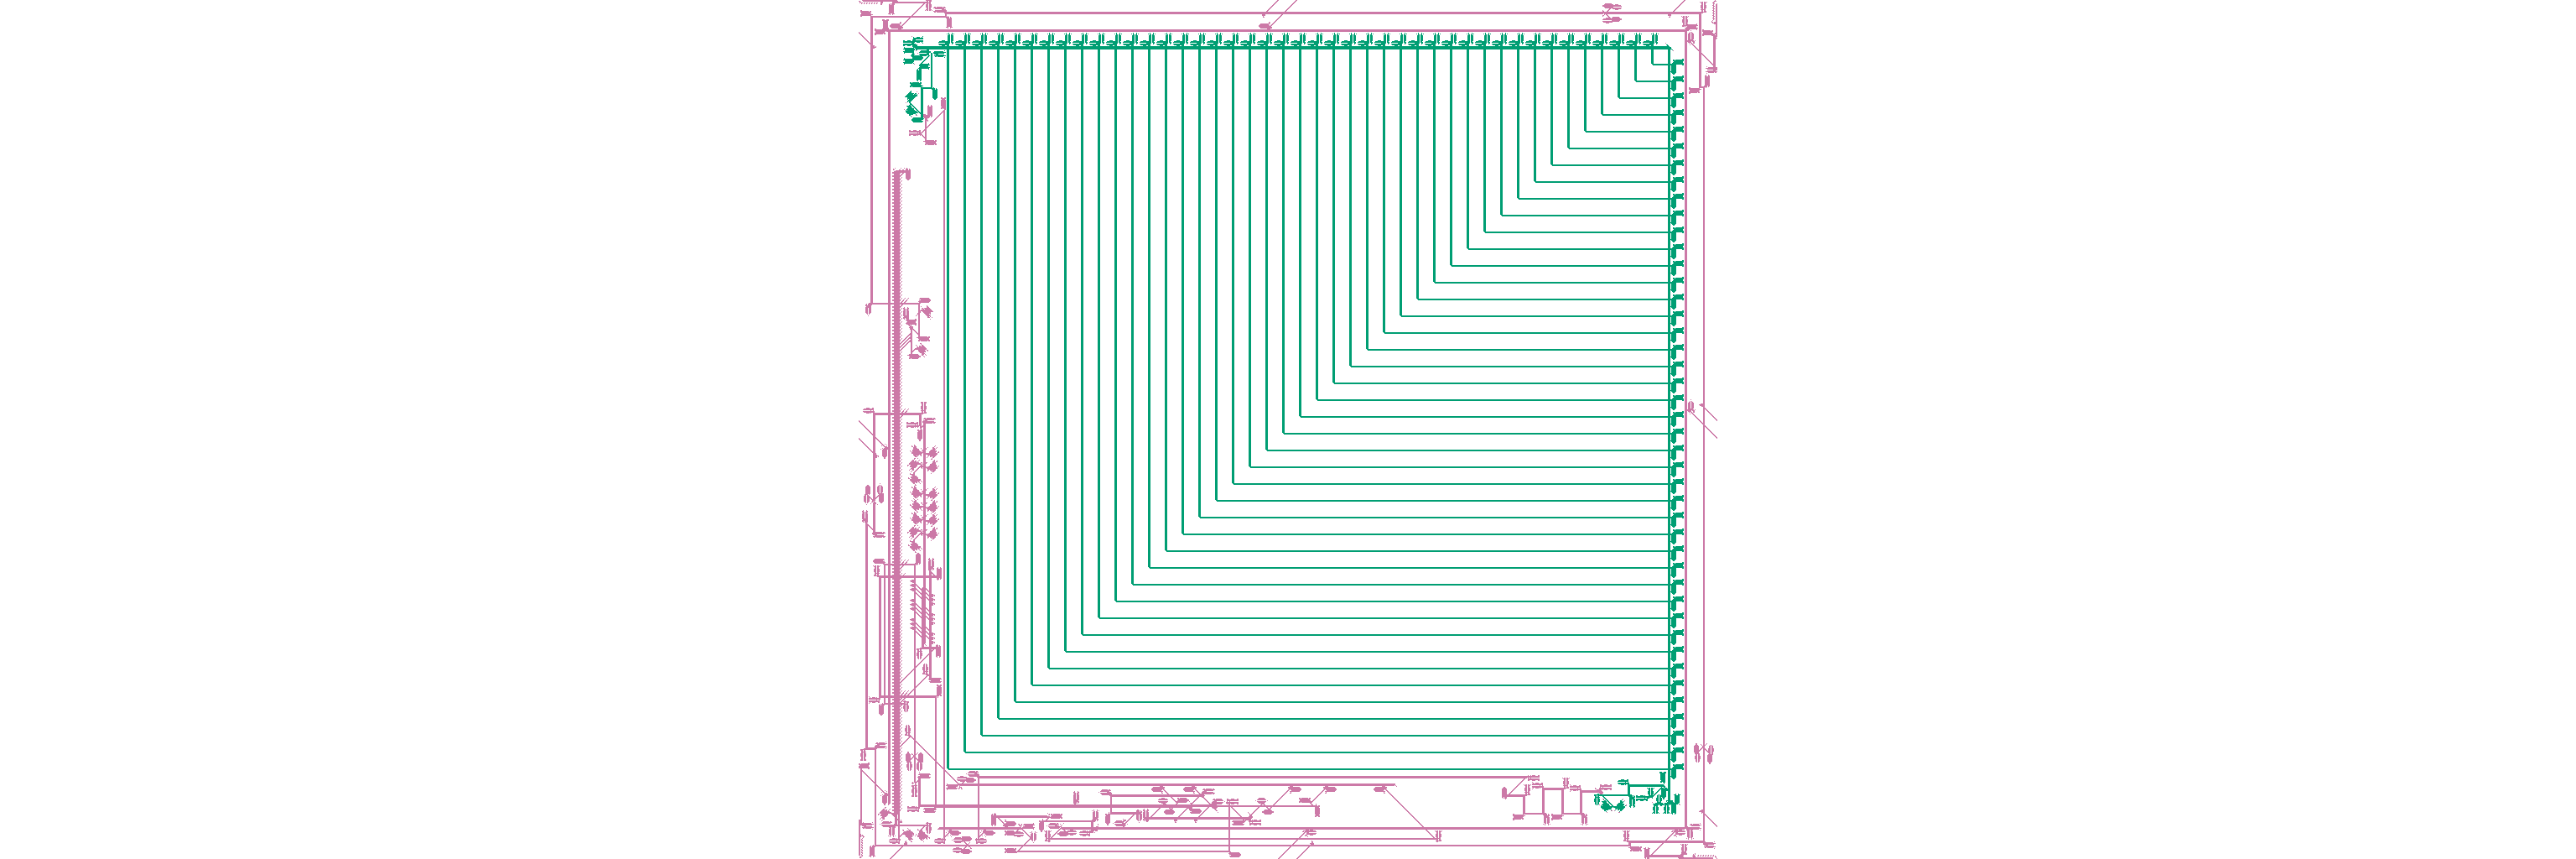
\includegraphics[width=\textwidth]{Figure 10.6.A}
\caption{A cell of Life simulated in Life}
\end{figure}
\noindent
When placed in a grid, these macrocells obey the computational rules of Life exactly at a slower time scale. Likewise, \textbf{NAND} logic gates and \textbf{NOR} logic gates are capable of antisimulating teach other as complement duals:
\begin{figure}[H]
\centering
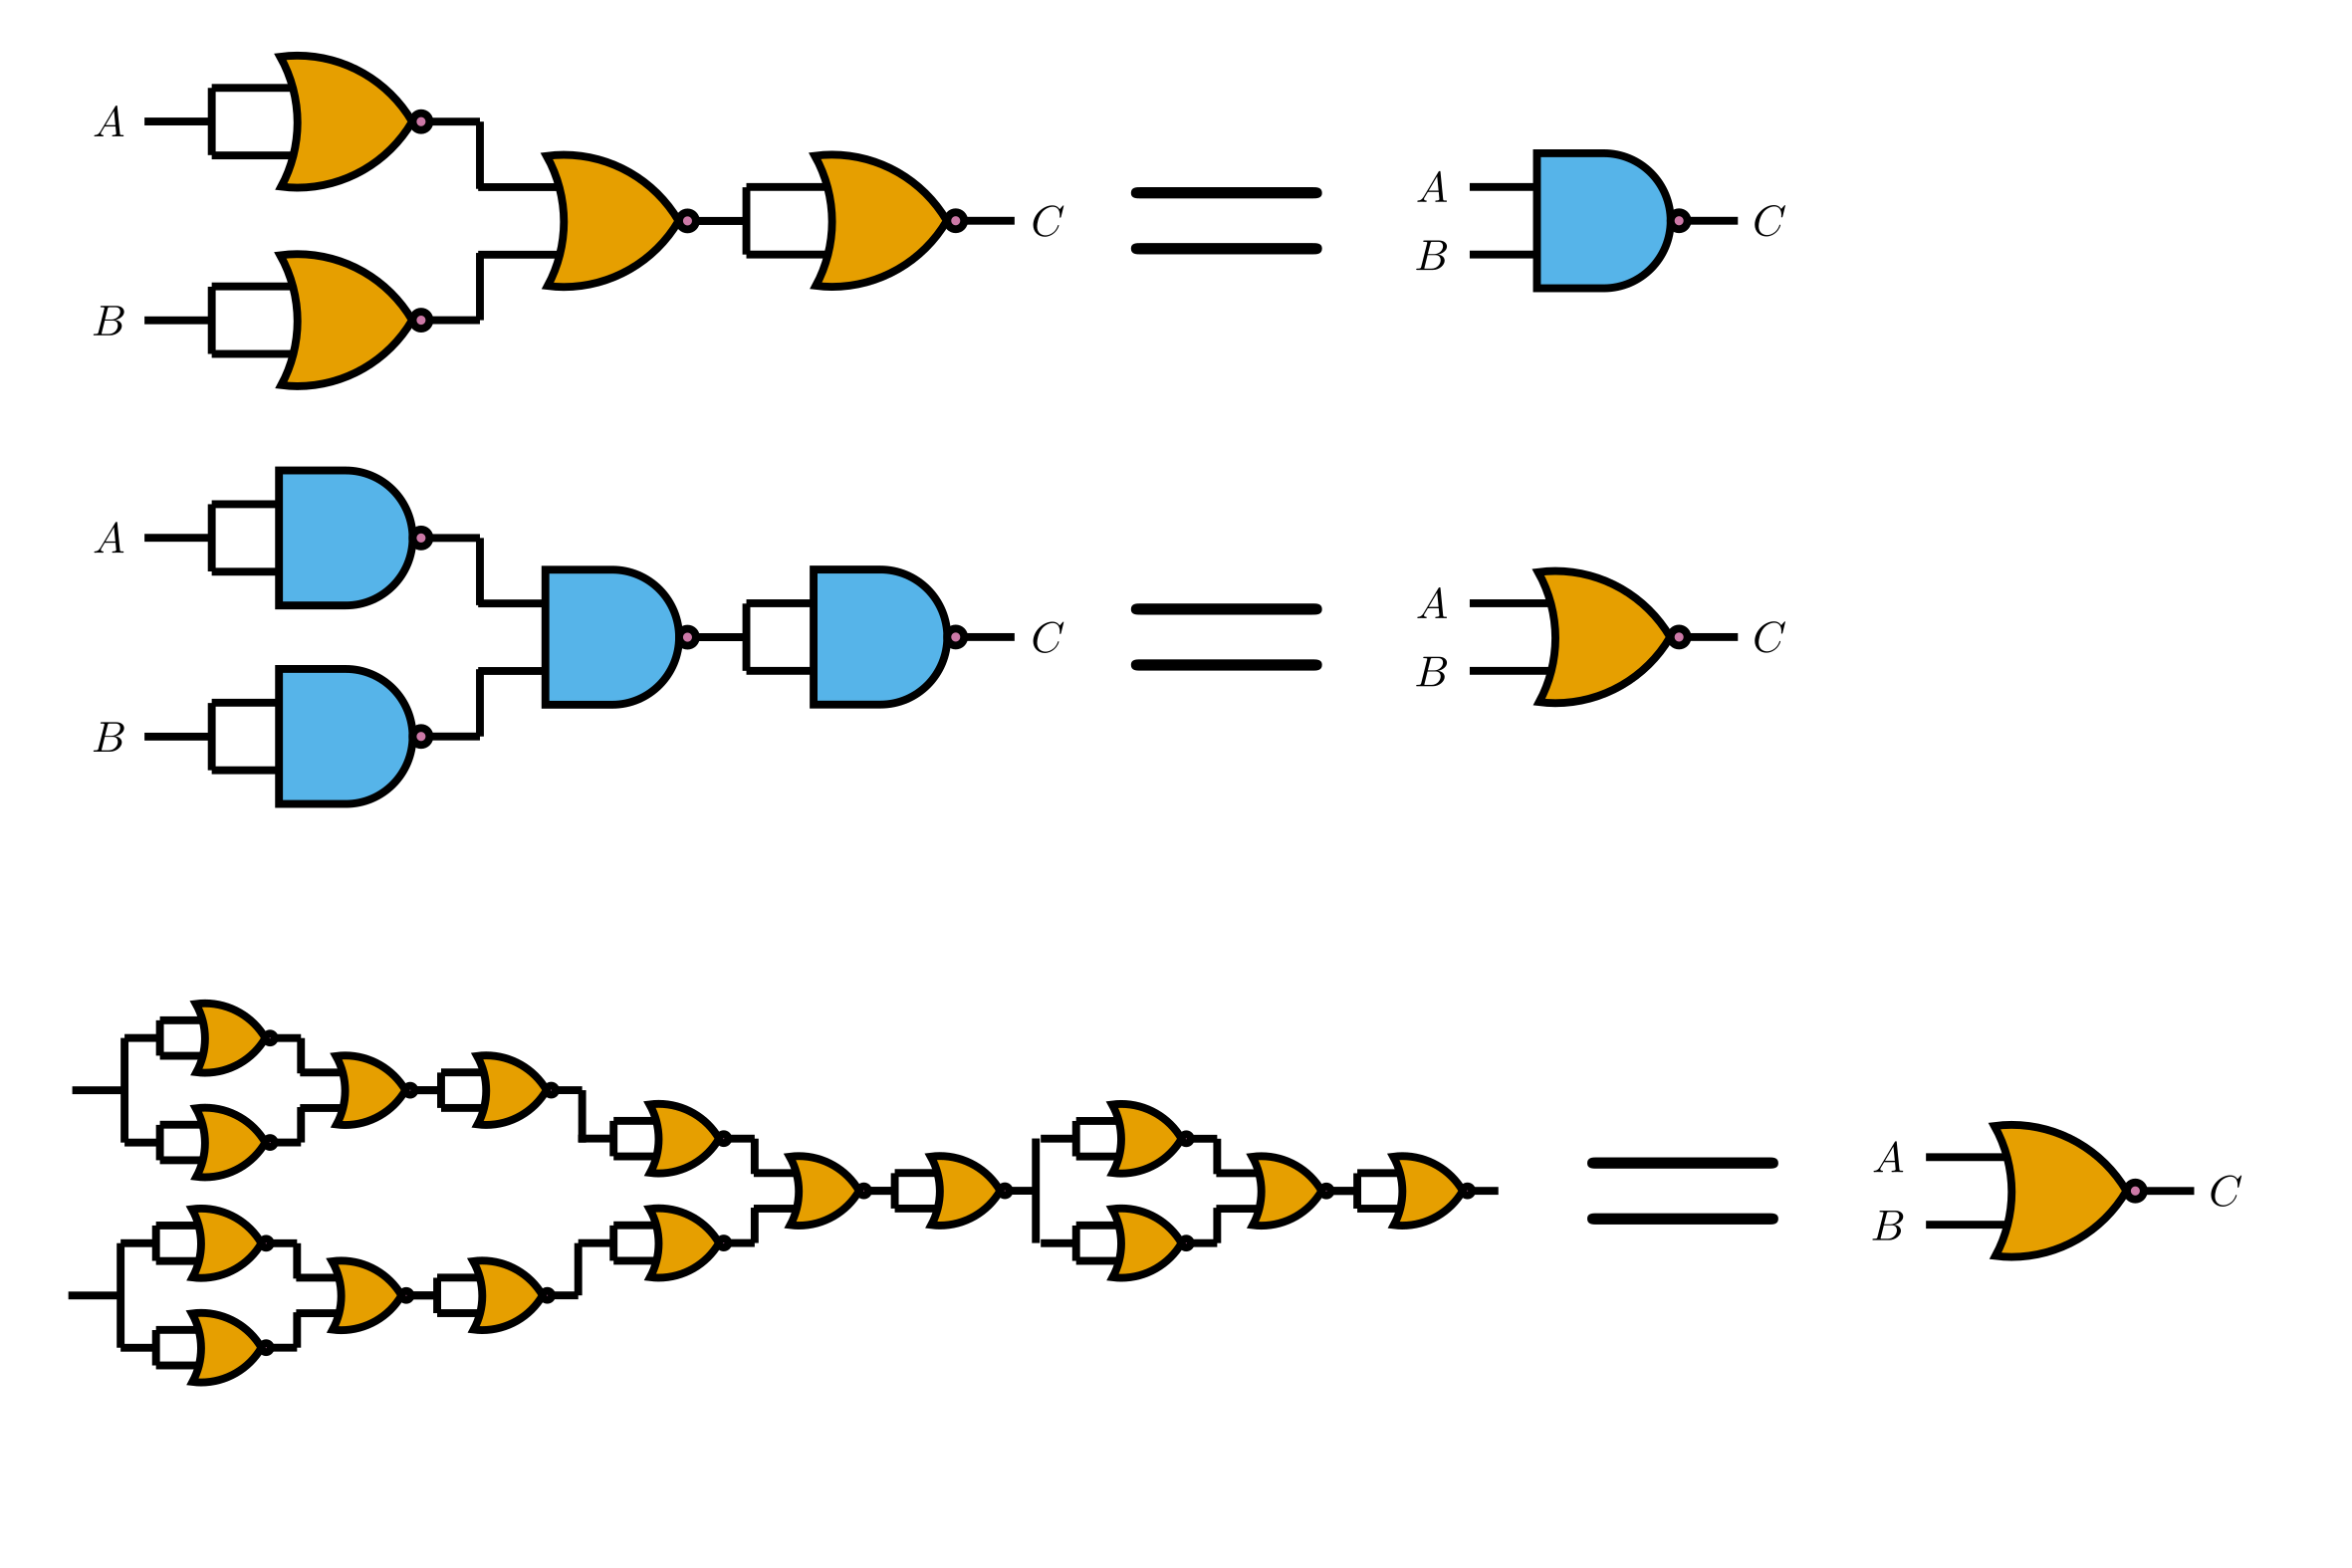
\includegraphics[width=\textwidth]{Figure 10.6.B}
\caption{An chain of NOR gates simulating itself}
\end{figure}
\noindent
These logic gates have an conjugate resimulation size of $4$ and conjugate resimulation time of $3$. Therefore, they have a resimulation size of $4^2$ and resimulation time of $3^2$.

This concept is related to the idea of \textbf{Hausdorff dimension}\index{Hausdorff dimension}, the measure of fractal dimension of a mathematical object or real object. Let us consider the Koch snowflake and name it our object $X$. The Koch curve is a recursive object with Hausdorff dimension $\log_3(4)$:
\begin{figure}[H]
\centering
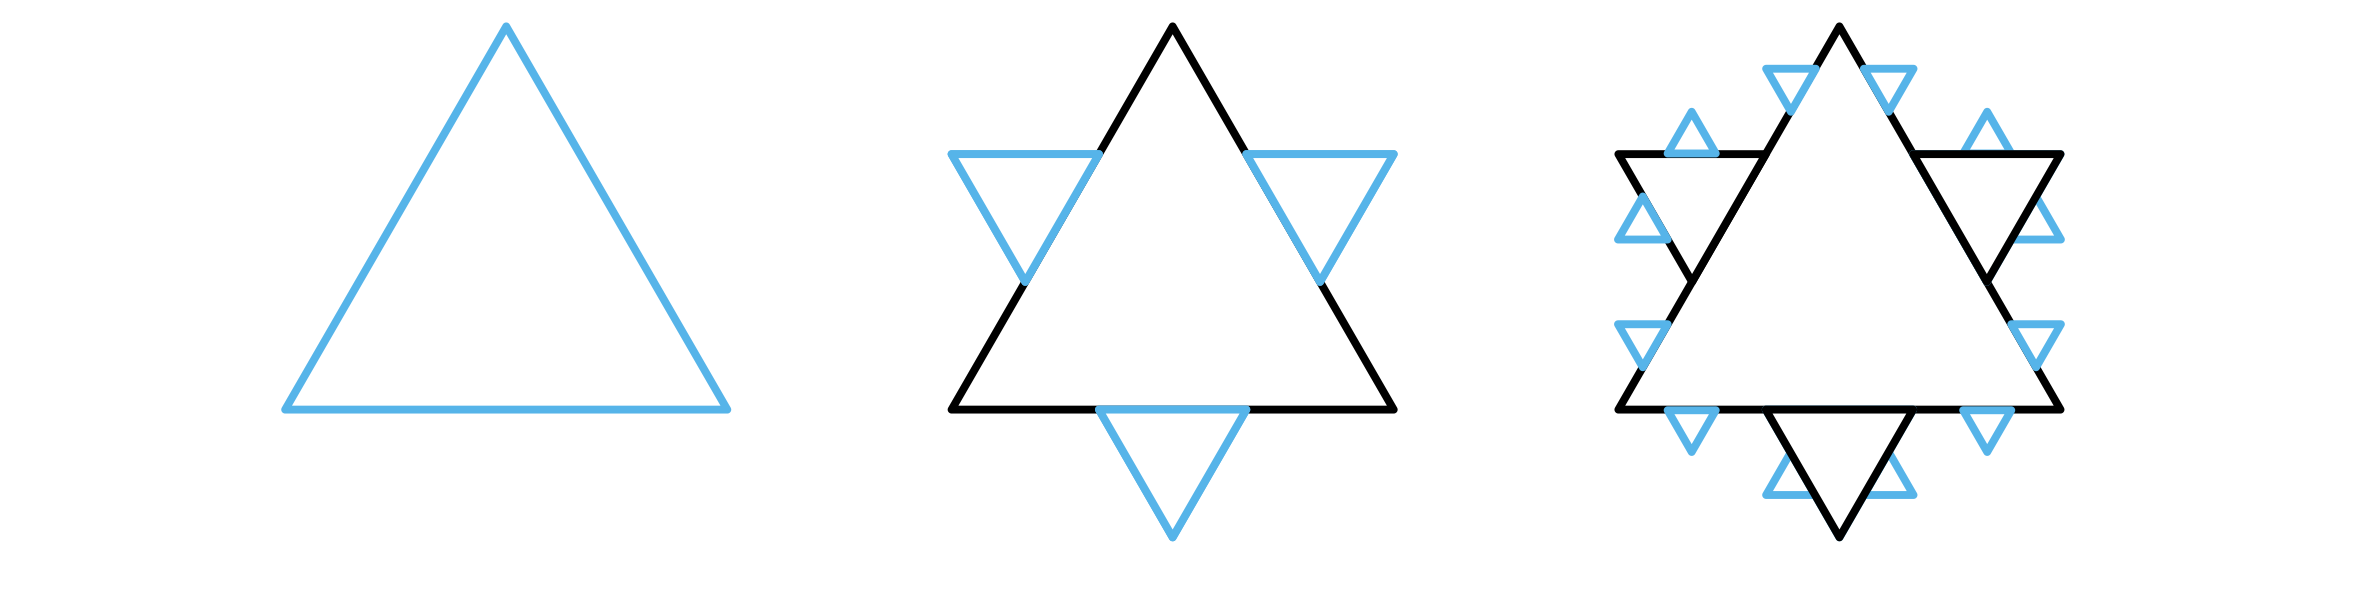
\includegraphics[width=\textwidth]{Figure 10.6.C}
\caption{Three iterations of the Koch snowflake}
\end{figure} \noindent
The number of sides after $n$ iterations is $N_n = 3 \cdot 4^n$ while its length for each size after $n$ iterations is $S_n = s / 3^n$. We shall consider $\frac{d}{dn} N_n$ to refer to the change in the count of the object, and we shall consider $\frac{d}{dn} T_n = \frac{d}{dn} S_n^{-1}$ to refer to the change in the time/length of the path. The Hausdorff dimension $\textnormal{dim}_H(x)$ is calculated as:
$$\frac{\frac{d}{dn} N_n}{\frac{d}{dn} T_n} = \textnormal{dim}_H(X) \frac{N_n}{T_n}$$
Using this formula, we can calculate the Hausdorff dimension of the Koch snowflake to be $\frac{\log(4)}{\log(3)} = \log_3(4)$.

Let us consider the \textbf{NAND}/\textbf{NOR} example involving logic gates. Suppose that we alternate between using \textbf{NAND} gates that simulate \textbf{NOR} gates and \textbf{NOR} gates that simulate \textbf{NAND} gates. We might say that we have a Hausdorff dimension of $\textnormal{dim}_H(X)= \log_3{4 \sigma}$ for each iteration. We are referring to $\sigma$ as some sort of conjugation operator.

Let $j$ be the hyperbolic unit in which $j^2 = 1, j \neq \pm 1$ just as the imaginary unit $i$ is given by $i^2 = -1$. The split-complex conjugate of a split-complex number $a+bj$ is $a-bj$, similar to how the complex conjugate of a complex number $a+bi$ is $a-bi$. If we are considering a conjugation operator $\sigma$ between \textbf{NAND} and \textbf{NOR}, then we should realize that $\sigma^2 = 1$, but $\sigma \neq \pm 1$. Thus, it behaves similarly to the hyperbolic unit of split-complex numbers.

Let us return to our \textbf{NAND}/\textbf{NOR} example. At each iteration, the object count is multiplied by $4$ and the temporal length is multiplied by $3$, but the object now behaves differently from before:
\begin{center}
\begin{tabular}{|c | c | c | c|}
\hline
$A$ & $B$ & $A \ \textbf{NAND} \ B$ $A \ \textbf{NOR} \ B$\\
\hline
$-1$ & $-1$ & $+1$ & $+1$\\
$-1$ & $+1$ & $+1$ & $-1$\\
$+1$ & $-1$ & $+1$ & $-1$\\
$+1$ & $-1$ & $-1$ & $-1$\\
\hline
\end{tabular}
\end{center}

Why should we care about the idea of resimulation? A Boolean mechanical system that is Turing complete can in theory simulate its rules at a larger scale, albeit with some randomness. It may also simulate other mathematical objects that simulate themselves. The question is how fractal dimensionality plays into repetitions of scale in some 3D transition rule.

\section{Approximate Rotational Invariance}
For a Boolean mechanical system $X_t = f(x,t)$, we are interested in transitions generated by the shift operator $S = e^{\frac{\partial}{\partial t}}$ upon $f(x,t)$ such that some transformation matrix $A$ upon cells $x$ in the system $X$ creates distributions that are approximately the same:
$$A^{-1} S A f \approx S f$$
The operator $A$ is an transformation upon the discrete coordinate positions $x$, specifically (Boolean) inversion, reflection, and rotation. For a Boolean random walk, it is trivially obvious that $A^{-1} S A f = S f$ in the case of Boolean inversion, reflection, and 90 degree rotations. We use $A$ because we may think of it as some kind of affine transformation, but we are not considering all affine transformations such as shearing and scaling.

We need special considerations for rotations that are not 90 degrees, a common problem faced regarding the rotation of low-resolution bitmap images. Here is an example of a circulant matrix algorithm using discrete circles:
\begin{figure}[H]
\centering

\includegraphics[width=\textwidth]{Figure 10.7.A}
\caption{A circulant matrix rotation of $\pi(3-\sqrt{5}+1)$ radians}
\end{figure} \noindent
This is an artwork depicting a black-furred kitsune with a white mask, a red kimono, and a handheld fan. This is the simplest lossless rotation algorithm for cubic lattices, permuting cells within a discrete circle layer. This results in distortion of outlines due to shearing between layers. 

The more common nearest neighbor rotation algorithm has the issue of removing key pixels such the eye highlight of the mask, and it likewise distorts outlines. Algorithms such as RotSprite (2007) and cleanEdge (2022) were designed to maintain outline integrity of pixel art.
\begin{figure}[H]
\centering

\includegraphics[width=\textwidth]{Figure 10.7.B}
\caption{A comparison of nearest neighbor, RotSprite, and cleanEdge $36^\circ$ rotation}
\end{figure} \noindent
Since these algorithms rely on upscaling, rotating, and downscaling the image, they often distort key pixels. At a $36^\circ$ rotation specifically, all of these algorithms lose the brighter red eye pixel in the mask. This is impossible with the circulant matrix algorithm since it strictly permutes cells.

The point being made here is that a transition rule $f$ that maintains perfect rotational symmetry in Boolean statistical mechanics is likely impossible. Defining a transition function $f$ that is rotationally symmetric that accounts for shearing of the discrete circle layers need only be approximate. A random walk converges to a Wiener process, which has continuous rotational symmetry. Boolean random walks likewise have this property of approximate rotational symmetry.

It is difficult enough to find symmetry with respect to Boolean negation for a cellular automata, but why should we care about arbitrary rotations? \textbf{Noether's theorem}\index{Noether's theorem} in physics states that every continuous symmetry of a system obeys a conservation law. Rotational invariance and its approximation is of interest for harmonic functions, particularly Boolean harmonics and macroparticle eigenclasses.

The Laplacian of a function $f(x, t)$ is given by $\nabla_x \cdot \nabla_x f(x) $ in which $\nabla_x$ is the gradient operator with respect to position vector $x$. The Laplacian is invariant with respect to rotation for continuous systems. We expect that discrete systems that have transition rules defined by the Laplacian are thus \textbf{approximately rotationally invariant}\index{approximate rotational invariance}. How can we formalize this notion for probability distributions on Boolean random fields on a square lattice?

The \textbf{Kullback-Leibler divergence}\index{Kullback-Leibler divergence} from empirical probability distribution $f(x)$ to theoretical probability distribution $g(x)$ is given by:
$$\textnormal{KL}(f, g) = \int\limits_{-\infty}^\infty \ln \bigg (\frac{f}{g} \bigg )f dx$$
It measures the relative entropy from $f$ to $g$, and is not a symmetric measure. The symmetric KL-divergence, or simply the divergence, between $f$ and $g$ is defined as:
$$f \Delta g = \textnormal{KL}(f, g) + \textnormal{KL}(g, f) = 
\int\limits_{-\infty}^\infty \ln \bigg (\frac{f}{g} \bigg )f dx + \int\limits_{-\infty}^\infty \ln \bigg (\frac{g}{f} \bigg)g dx$$
We desire that the symmetric KL-divergence $f \Delta g$ is bounded by some error constant $\varepsilon > 0$ whenever we perform some kind of pixel rotation that will induce some sort of divergence in distribution

Let $R_{\max}$ be a rotation transformation upon a position space $x$ upon the integers $\mathbb Z^d$ such that the divergence $f \Delta g$ is maximized:
$$R_{\max} = \underset{R \in \mathcal R}{\textnormal{argmax}} \ (f_1 \Delta g_1)$$
$$\varepsilon = \underset{R \in \mathcal R}{\max} \ (f_1 \Delta g_1)$$
in which $g_t = g(x, t)$ is the probability distribution given by $g_t = R^{-1}P^t R f_0$ and $\mathcal R$ is the set of valid discrete rotation approximation transformations. Due to our transition matrix representation, $f_t = P^t$ and $f_0 = I$. Our rotation matrix $R$ represents a permutation of the transition matrix $P$. This means that:
$$g^t = R^{-1} P^t R$$
represents rotating, advancing, then unrotating our matrix. We will discuss what denotes a lossless discrete rotation in higher-dimensions later in the section. 

We know that $f_t \Delta g_t$ is minimized for 90 degree rotations upon a grid, or rather $\theta \mod \frac{\pi}{2}$ rotations in which the continuous rotation is represented by $e^{i \theta}$. We assume that there is some rotation angle for which the symmetric divergence is maximized for a single time step.

We say that the transition rule for $f$ is approximately rotationally invariant if:
$$a_t = (PR)^t f_0$$
$$b_t = P^t R^t f_0$$
$$a_t \Delta b_t < \varepsilon, \quad \forall t > 0, t \in \mathbb Z$$
In other words, we are asking that the error $\varepsilon$ is small for \textit{rotating and advancing} $t$ times in series versus \textit{rotating} $t$ times then \textit{advancing} $t$ times. We want the symmetric KL-divergence to be less in future time steps than the error constant $\varepsilon$, in which $\varepsilon$ was computed for a single time advancement for each configuration eigenstate $\hat X_i$. 

Why this specifically? If you naively prefer:
$$f_t \Delta R^{-1} P^t R f_0 < \varepsilon, \quad \forall t > 0, t \in \mathbb Z$$
then you run into the dominance of the stationary distribution eigenvalues. Remember that a stochastic matrix has $|\lambda| \leq 1$ for all of its eigenvalues. A Boolean random walk will quickly erase its errors if you only rotate once due to the dominant eigenvalue of $\lambda_1 = 1$, but serially rotating by some maximally erroneous angle is stricter.

This reminder about the stationary distribution actually poses an interesting point about how we should go about tackling the problem for Boolean random walks specifically. Let $P^*$ be similar to stochastic matrix $P$ except that it is for two-step transitions given by $P^2$ and we have folded the even-odd duplicates (given by Boolean negation) together. Then the eigenvector $\phi^*_1$ is the stationary distribution with eigenvalue $\lambda^*_1$. 

What can we say about $\phi^*_1$ and its relation to $R^{-1} P R \phi^*_1$? We know that the stationary distribution necessarily obeys $P \phi^*_1 = \phi^*_1$, a result of its time invariance. What can we say about the symmetric divergence:
$$R^{-1} P R \phi^*_1 \Delta \phi^*_1$$
for arbitrary rotations $R \in \mathcal R$? Ideally, it is the case that the maximum error bound $\varepsilon$ is low even for the maximum error rotation $R_{\max}$.

We should take care to notice that the error in distribution is primarily a result of the central fixed point of rotation and shearing between layers:
\begin{figure}[H]
\centering
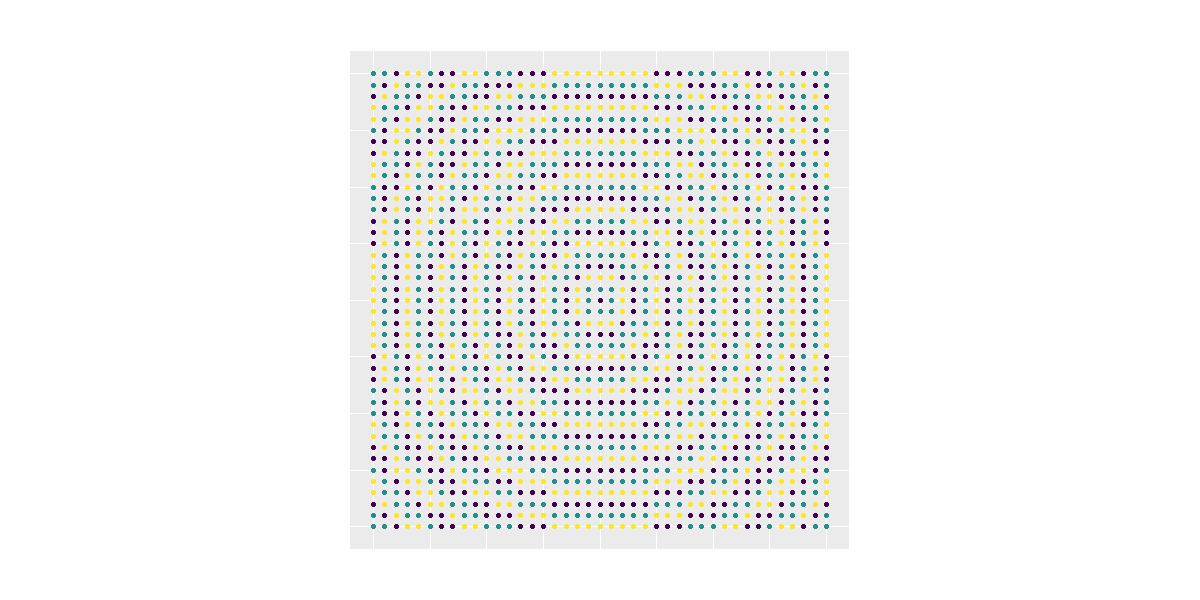
\includegraphics[width=\textwidth]{Figure 10.7.C}
\caption{The circular layers of a rotation}
\end{figure} \noindent
The layers of a circle of sphere rotate at different rates given by some hypercomplex numbers. If the dimensionality of $x$ is given by $d$, then we need the Cayley-Dickenson construction of hypercomplex numbers with dimension $2^{d-1}$. This skipping between layers results in the error in distribution measure by divergence $f \Delta g$, but the error between layers should diminish as the hypersphere layers approaches infinity.

The voxel hypersphere layer (centered at 0) of radius $r$ is the union of cells in which $(r-.5)^2 > x \cdot x > (r+.5)^2$ for some $d$-vector x. Only cell midpoints that are enclosed by the bounding circles are allowed in the layer. Each point may be represented by a hypercomplex vector representing some angle. If you look carefully in the 3D case, each 3D layer is numerous 2D layers offset by some position:
\begin{figure}[H]
\centering
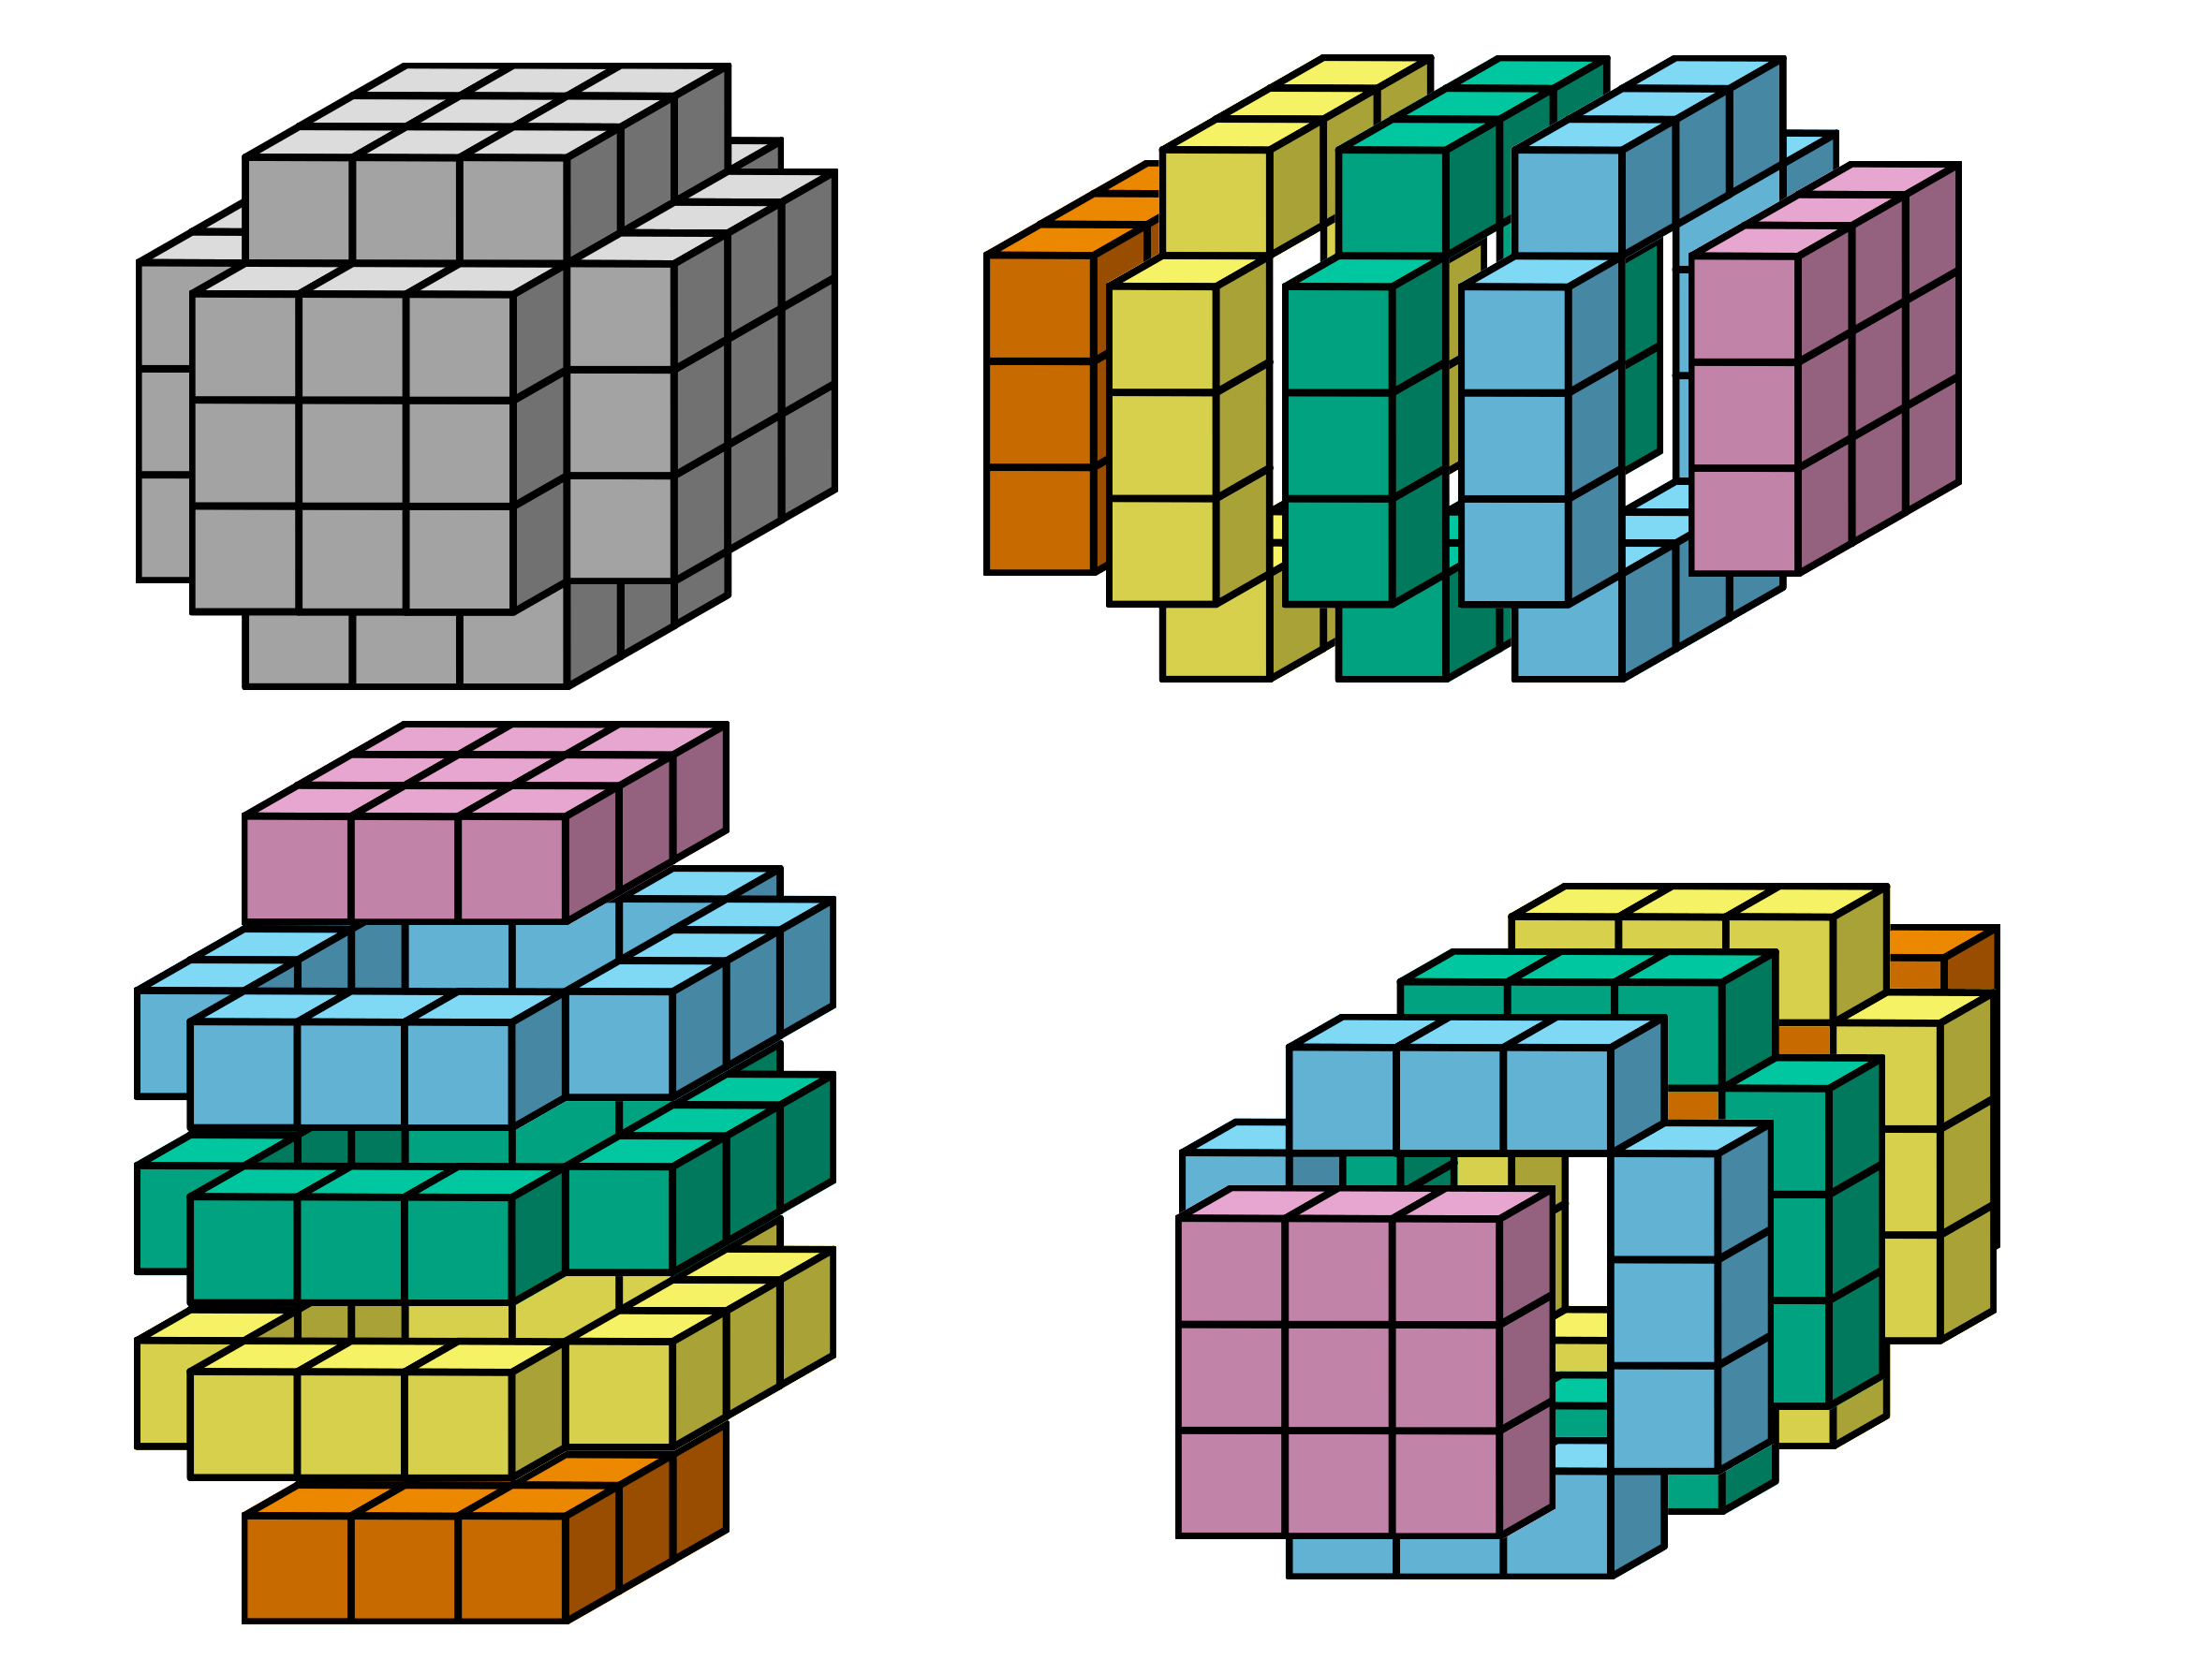
\includegraphics[width=\textwidth]{Figure 10.7.D}
\caption{The discrete rotation layers of a 3D sphere}
\end{figure} \noindent
This essentially means that there is a restriction to the 3D shifts as they correspond to compositions of 2D shifts, and 4D shifts as compositions of 3D shifts and their 2D shifts and so on. Using hypercomplex numbers outpaces the number of dimensions in the original vector $x$, so we should use a different method to map points. If there are $n$-points in each hypersphere layer, then some $n^2$ matrix indicates which mapping minimizes the squared error between the original position vector $x$ and the new position vector $x' = xe^{ai}$ in which $a$ is the vector coefficients modular coefficients and $i$ is the basis vector the the hypercomplex algebra.

This should give us some inkling as to what macroparticle eigenclasses must behave like in order to be stable for Boolean statistical mechanics. A \textit{shell} about some \textit{core} whose probability distribution has \textit{approximate rotational invariance} as it \textit{permutes} into a \textit{group} of states that tend to \textit{cycle} about and between each other through time. A shell is a composition of spherical layer. Since approximate rotational variance is given by some modular arithmetic of a hypercomplex algebra, it is related to crytography. It stop existing because its \textbf{crytopgraphic shell}\index{crytographic shell} is either decrypted or compromised. Macroparticles that persist for a long time are quite stubborn, such as an electron. 

The idea of a cryptographic shell is important because its core maintains some rather small amount of data beneath Shannon's limit. In theory, the cryptographic shell should expand memory usage to maximize the stability of the data core up to the Shannon's limit of the vacuum. This theory presents an ambiguity in the interpretation of an electron: We are not quite sure if the electron we understand is the thing \textit{in} a shell or if the electron \textit{is} a shell. Virtual particles must be unstable because their existence demands an entropy rate that surpasses the local Shannon's limit.

The question remains if it is possible that the interior of a macroparticle as being hollow. We stated that we like the idea of a macroparticle being resistant to noise, but perhaps that applies to the inside being a hollow of noise as opposed to merely the outside. We stated that we like the idea of it being radially harmonic, but now we have a somewhat more rigorous condition. We desire that a shell $f(x)$ obeys the expectation of $\nabla_x \cdot \nabla_x f(x) \approx 0$. Instead of being a harmonic function, we want shells that are semi-stable due to being \textit{almost} harmonic functions.

\section{Non-Local Information}
Suppose that you have a Boolean random walk system initialized as $X_0$ and multiply it by a checkerboard state:
\begin{figure}[H]
\centering
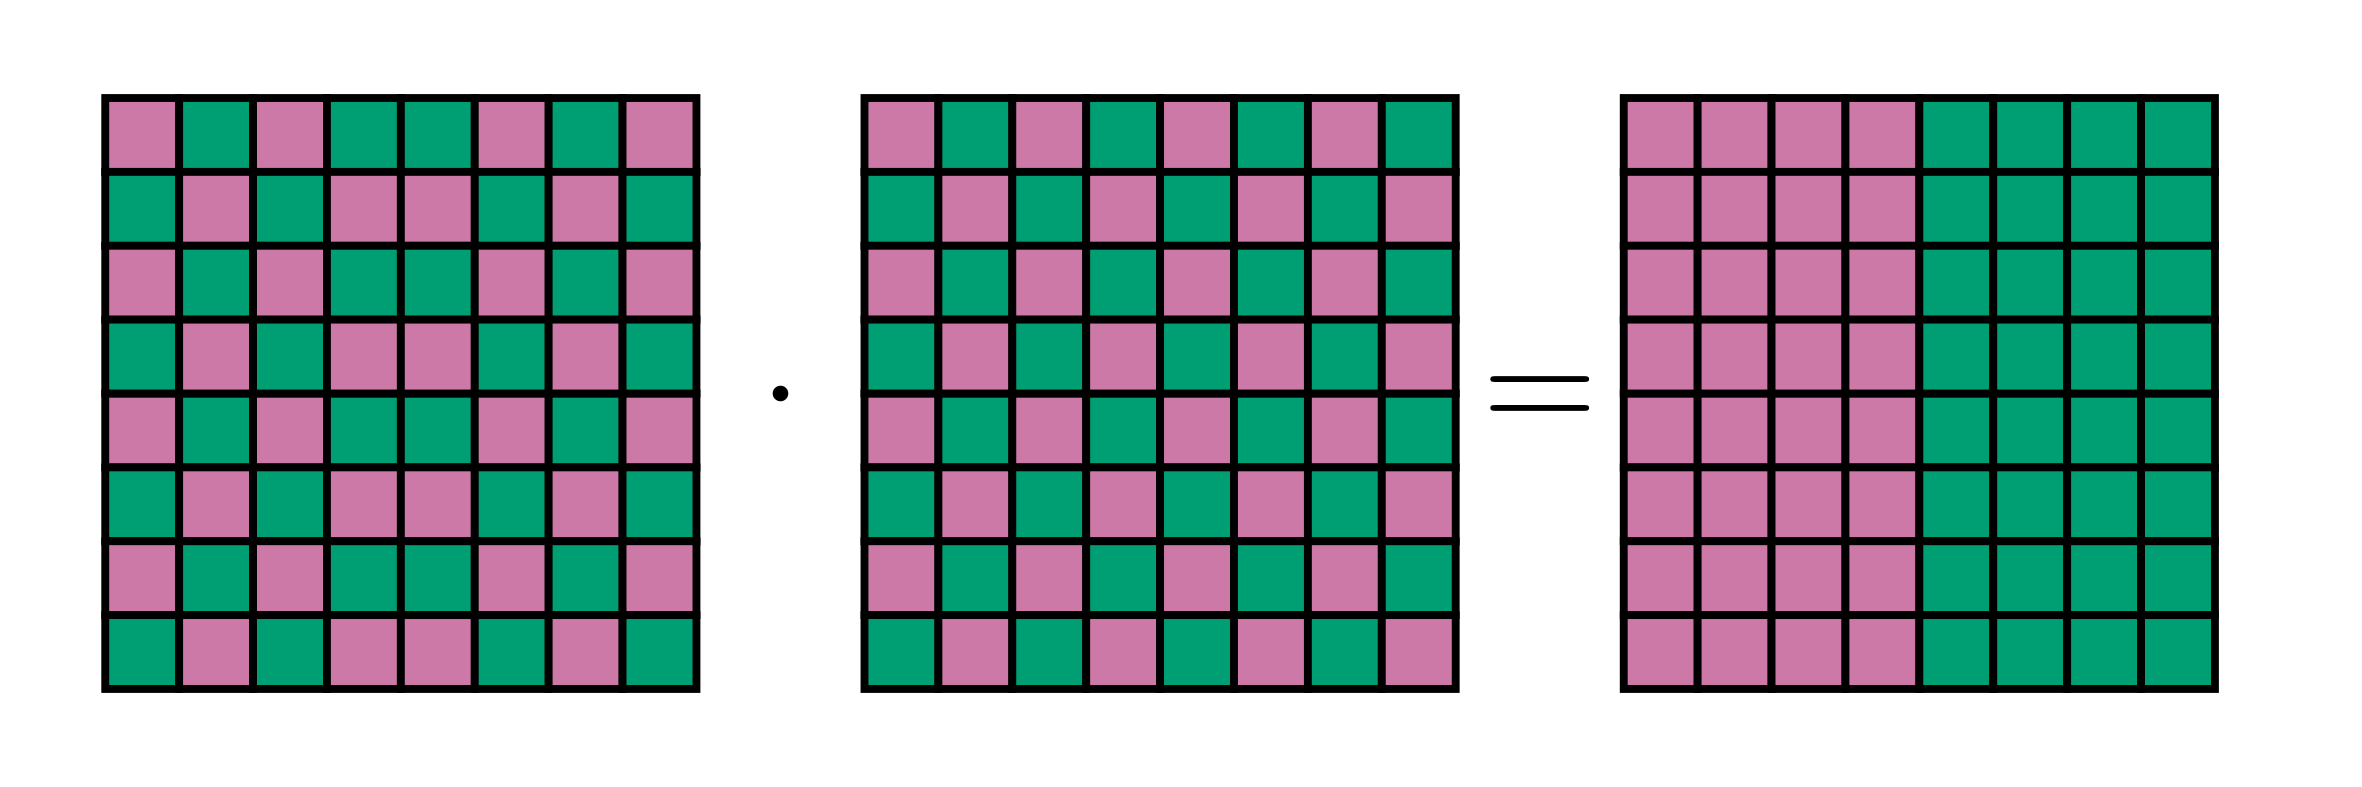
\includegraphics[width=\textwidth]{Figure 10.8.A}
\caption{Adjacent but opposing checker domains are statistically independent in a Boolean random walk}
\end{figure} \noindent
\noindent % A BRW system, a checkerboard state, and its multiplication
A continuous series of $+1$ or $-1$ cells form a volume whose conditional probability depends on every cell in the volume. Two adjacent volumes of $+1$ and $-1$ parity each are \textit{statistically independent} because a Boolean random walk may not occur across their boundaries.
\begin{figure}[H]
\centering
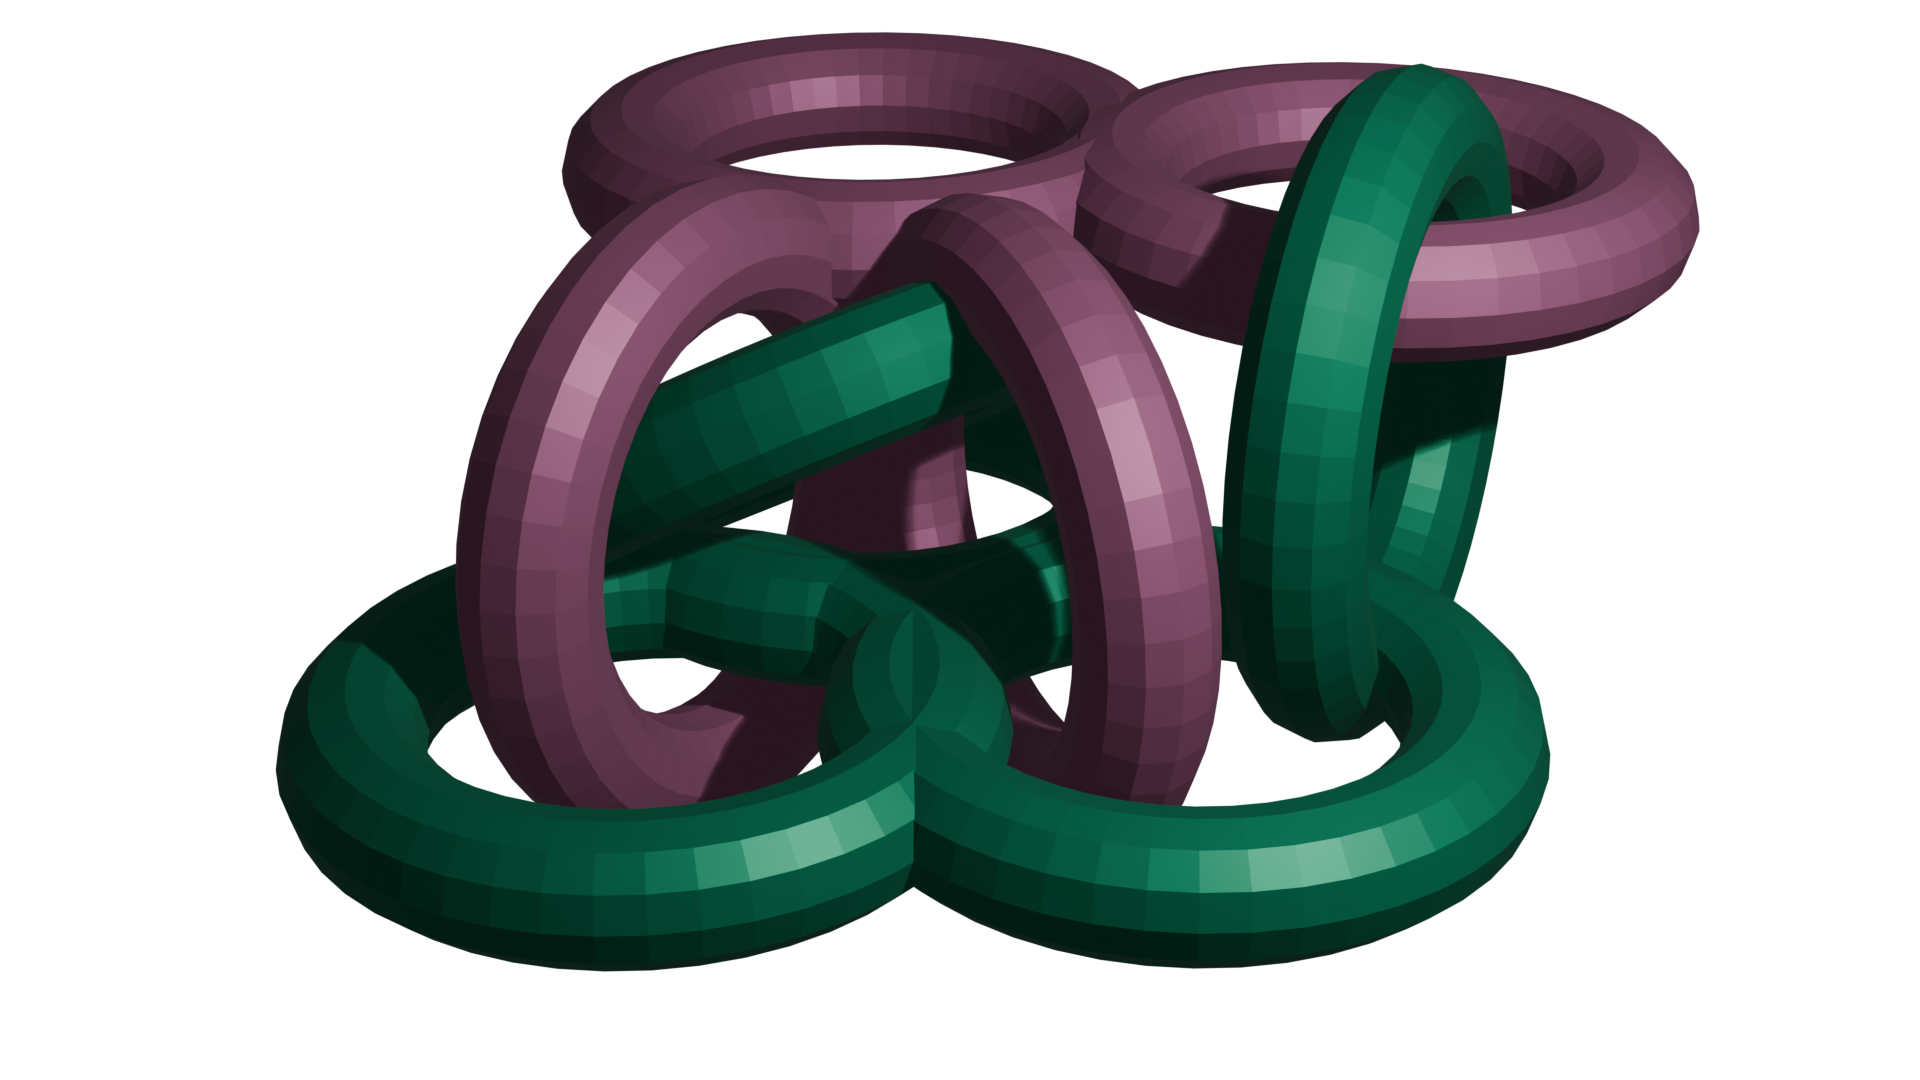
\includegraphics[width=\textwidth]{Figure 10.8.B}
\caption{Interwoven yet independent checker topologies in 3D}
\end{figure} \noindent
\noindent % Before and after checkerboard multiplication, showing inability to cross
As discussed in \textit{\S 7.8 Discrete Topology}, the volume has a boundary called a topology, and the complexity of the topology can be described by its Euler characteristic $\chi$. Since it is a connection of $d$-cubic cells, we can guarantee that it is an orientable surface, unlike a M\"{o}bius strip.

This long-range dependence of checkerboard states in a Boolean random walk simulation might be considered non-local. This is only for a single time step from $X_0$ to $X_1$. For $X_t$, you have to consider every single possible \textit{spatiotemporal} checkerboard chain that may have occurred between two cells since $t=0$. This means that information travels faster than the speed of any individual random walker, and this is due to the way that we have defined how to resolve a Boolean random walk: maximal independent sets in which one bit flip precludes many others.

Two cells of a Boolean random walk are non-locally dependent at time $t$ if there is a non-zero probability of a enclosure within a ``checkerboard topology'' that links back at some time point $t^*$ in the past, in which $t^* < t$. If you consider how a $2$-dimensional Boolean random walk evolves in time as a $3$-dimensional array then multiply that array by a $3$-dimensional checkerboard pattern, then you may have multiple continuous volumes assigned a parity of $+1$ or $-1$. If you have a realized simulation and consider a single volume, cells at different time steps in the same checkerboard within that volume have definitely influenced each others' probabilities.

\chapter{State Space Analysis}
\section{Motivations for State Space Analysis}
In previous chapters, we established the heuristics and theory behind how we might observe abstractions of familiar concepts. State space analysis seeks a more thorough and rigorous way to define and explain observations. This comes directly at the cost of computability using a computer, be it a personal or a lab supercomputer. Absolute knowledge requires either infinite computing power or formal mathematical relations using symbolic logic. A Boolean mechanical system and programs on a computer are more than merely sets of states: They are about \textit{how} those states flow between each other.

If omniscience of a Boolean mechanical system is impossible, then we must endeavor to understand it using a variety of tools and tricks. Even though the state space graph of games like chess or weiqi (Go) are impossibly large, we can hope to understand those games using tools and heuristics. Instead of studying global patterns that lead to win or loss exactly, we can focus on local patterns or structures that beget advantage or disadvantage. We can likewise focus on some core ideas derived from statistics, physics, and little ideas derived from myself.


\section{Boolean Mechanics Expected Values}
In statistical inference, we have the following relations for expectations for a probability distribution $f(x)$:
$$\mathrm{E}(1) = \int\limits_{x \in X} f(x)dx = 1$$
$$\mathrm{E}(X) = \int\limits_{x \in X} x \cdot f(x)dx$$
$$\mathrm{E}(g(X)) = \int\limits_{x \in X} g(x) f(x)dx$$
Quantum mechanics uses a slightly different notation to avoid the use of the letter $E$ which is often used for energy:
$$\langle I \rangle_\psi = \langle \psi | I | \psi \rangle = \int\limits_{x \in X} \psi^{*}(x) I \psi(x)dx$$
$$\langle X \rangle_\psi = \int\limits_{x \in X} \psi^{*}(x) x \psi(x)dx = \int\limits_{x \in X} x \cdot \psi^{*}(x) \psi(x)dx$$
As a reminder, a wavefunction $\psi(x)$ has the following relation $\psi^*(x) \psi(x) = f(x)$. 

We wish for a similar definition for Boolean statistical mechanics as quantum mechanics. The notation and definition should make intuitive and formal sense. If we define the eigendecomposition of a stochastic transition matrix $P^t = \Phi \Lambda \Phi^{-1}$, then expectations should be given by:
$$\mathrm{E}(A) = \Phi A \Phi^{-1} = \langle A \rangle$$
How sensible is this definition? Let us look at some examples:
$$\mathrm{E}(I) = \Phi I \Phi^{-1} = \Phi \Phi^{-1} = I$$
$$\mathrm{E}(\Lambda^t) = \Phi \Lambda^t \Phi^{-1} = P^t$$
$$\mathrm{E}(X_t) = \Phi \Lambda^t X \Phi^{-1} = P^t \cdot \mathcal X$$
$$\mathrm{E}(X_t | X_0) = y_0 P^t \odot \mathcal X$$
$$\mathrm{E}(\Phi) = \Phi \Phi \Phi^{-1} = \Phi I = \Phi$$
$$\mathrm{E}(\Phi) = \Phi \Phi^{-1} \Phi^{-1} = I \Phi^{-1} = \Phi^{-1}$$
They also make sense if stated as a sentence. Recall that the eigenvalues correspond to the shift operator:
$$\Lambda_\sharp y_t = e^{\frac{\partial}{\partial t}} y_t = y_t P = y_t \langle \Lambda \rangle$$
We may say that the shift in time by $\tau$ time steps gives the probability distribution after $\tau$ time steps. It is \textit{linguistically tautological}.

Notice how even in the previously mentioned quantum mechanics definition that $\langle \psi(x) \rangle = \psi(x)$. We should also be specific when we use the position operator $X = \mathrm{E}^{-1}(\mathcal X)$, thus pushing our state space operator $\mathcal X$ outside the expectation function. Thus $\mathrm{E}(X \Lambda_t)$ reads as ``the expected Boolean configuration at time $t$''. Expectations without some initial state vector $y_0$ will produce the entire family of states, as $y_0$ is some sort of selector.

We now have a definition of expectation that seems obvious in hindsight. We can calculate familiar statistics for a multitude of initial states, and we can condition upon an initial state by choosing one of the rows.
$$\mathrm{E}(X_t) = P^t \odot \mathcal X$$
$$\mathrm{Var}(X_t) = P^t \odot \bigg [ \mathcal X - \sum\limits_{j} \mathrm{E}(X_t)^2 \bigg ]$$
Variance is more complicated to calculate because we need to consider the expected value of the specific row. We need to employ the same summation trick across each row for entropy rate $S$.
$$S(X_t) = -\sum\limits_{j} P^t \odot \ln(P^t)$$
$$H(X_t) = \ln \bigg (\frac{X_{t+1}}{X_{t}} \bigg ) / (\pi i) = H_t$$
$$T(X_t) = \frac{\Delta_t S_t}{\Delta_t H_t} = T_t$$
$$\beta(X_t) = \frac{\Delta_t H_t}{\Delta_t S_t} = \frac{1}{T_t} = \beta_t$$
We have expectation, variance, entropy $S$, Hamiltonian energy $H$, temperature $T$, and coldness $\beta$ (inverse temperature). Temperature $T$ and inverse temperature $\beta$ are usually defined in terms of the partial derivative $\partial$ when working with continuous systems, but the finite difference operator $\Delta$ is more appropriate in this context.

Justifying proper definitions for thermodynamic beta $\beta_t$ and the Hamiltonian energy $H_t$ is more because of the ambiguity with how to interpret them. How is it that temperature and inverse temperature can be defined without the motion of particles that we may be familiar with? How do we define the partial derivative of energy: geometrically or arithmetically? We shall discuss this later in the chapter during \textit{\S 11.5 Boolean Thermodynamics}.

\section{Boolean Hamiltonians}
Consider the Hamiltonian of the Ising model in terms of Boolean mechanics:
$$H(\sigma) = - \sum\limits_{i \ \textnormal{near} \ j} J_{(i, j)} \sigma_i \sigma_j \rightarrow H(x) = - \sum\limits_{i \ \textnormal{near} \ j} \chi_{(i, j)} f(x_i) f(x_j)$$
If $f(x_i) = f(x_j)$, then the energy between two adjacent cells is negative. If $f(x_i) = -f(x_j)$, then the energy between them is positive. Consider the representation transformation of the Boolean set $\{-1, +1\} \rightarrow \{1, 0\}$:
$$\{-1, +1\} = e^{\{1, 0\} \pi i} \iff \{1, 0\} = \frac{\ln(\{-1, +1\})}{\pi i}$$
This gives us a convenient way to move between these two representations of parity $\{-1, +1\}$ and angle $\{0, 1\}$ in unit half-cycles (as opposed to radians).

We know that a Boolean random walk's stochastic transition matrix $P$ has eigenvalues has eigenvalues $\lambda_1 = 1$ and $\lambda_2 = -1$. We want to have:
$$\hat H = \frac{\partial}{\partial t} \cdot \frac{1}{\pi i} = \ln(\Lambda) \cdot \frac{1}{\pi i}$$
$$e^{\hat H} = \bigg ( \frac{X_{t+1}}{X_{t}} \bigg ) ^{\frac{1}{\pi i }} \iff \hat H = [\ln(X_{t+1}) - \ln(X_{t})] \cdot \frac{1}{\pi i}$$
$$\iff \mathrm{E}(\hat H) = \mathrm{E}[\ln(X_{t+1}) - \ln(X_{t})] \cdot \frac{1}{\pi i}$$
This makes is so that the Hamiltonian operator $\hat H$ generates a probability distribution of the relative rotation upon $(x, t)$. We cannot move the expectation inside because of the dependency upon the transition experienced from $X_t$ to $X_{t+1}$. In most cases, $\mathrm{E}(g(X)) \neq g(\mathrm{E}(X))$.

We should state that if $p_t$ is the probability that a cell rotated at time $t$:
$$\mathrm{E}(\hat H_0) = p_0 = 1$$ 
$$\mathrm{E}(\hat H_1) = \frac{p_1}{p_0}$$
$$\mathrm{E}(\hat H_2) = \frac{p_2}{p_1}$$
We cannot define the specific Hamiltonian as $\mathrm{E}(X_{t+1}) / \mathrm{E}(X_t)$, it instead must be $\mathrm{E}(X_{t+1} / X_t)$. We need to condition on all possible initial states and transitions of $\mathrm{E}(X_t)$. The action $\mathcal S$ is given by the summation: 
$$\mathcal S(t) = E(H_0 + H_1 + ...+ H_t)$$
As discussed in \textit{\S 9.5 Issues in Defining Energy}, a Boolean signal of $f \in \{-1, +1\}$ has energy proportional to signal length, but \textit{changes} in the signal $f$ are measurable.

Why should we define the Hamiltonian this way specifically? Consider the $2 \times 2$ oscillator for a Boolean random walk:
\begin{figure}[H]
\centering
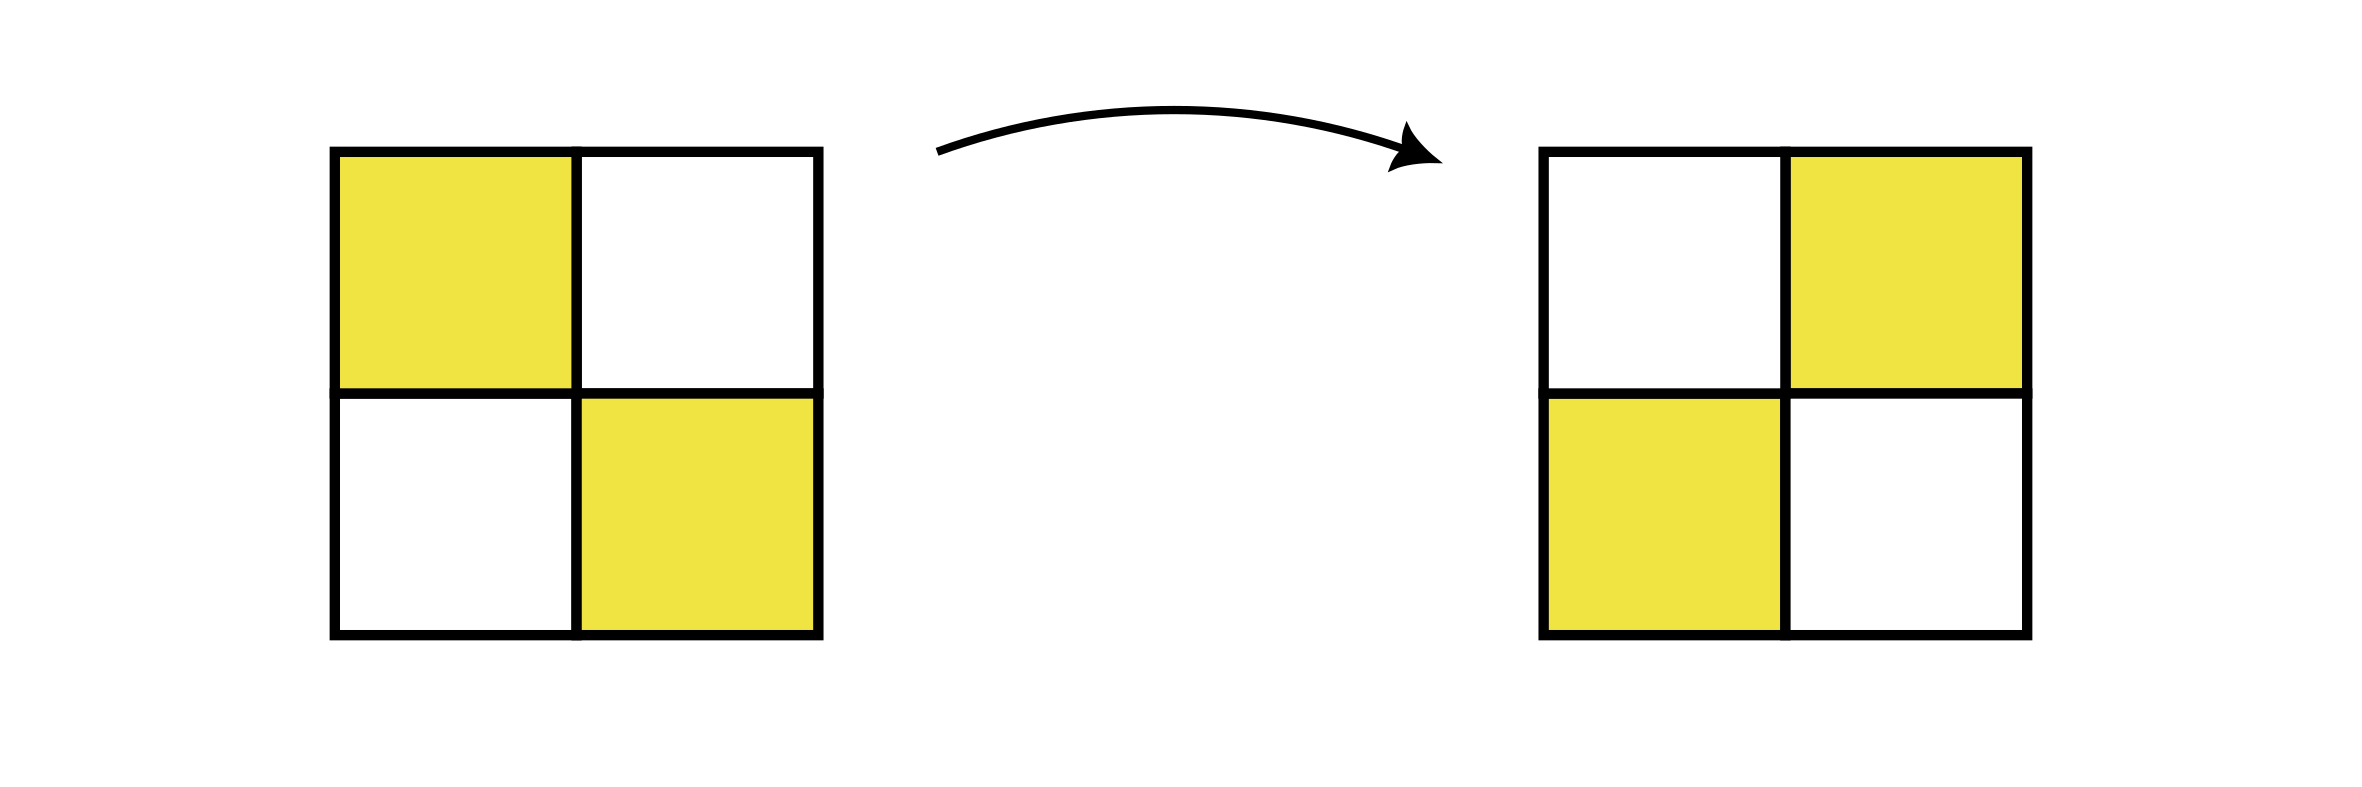
\includegraphics[width=\textwidth]{Figure 11.3.A}
\caption{An average of $4/4$ cells rotating}
\end{figure}
\noindent
Every cells experiences a rotation by $e^{\pi i}$ and there are 4 cells. By defining the Hamiltonian operator this way, we see that $\frac{4}{4}$ cells in our system have rotated. If we consider another transition rule other than Boolean random walks:
\begin{figure}[H]
\centering
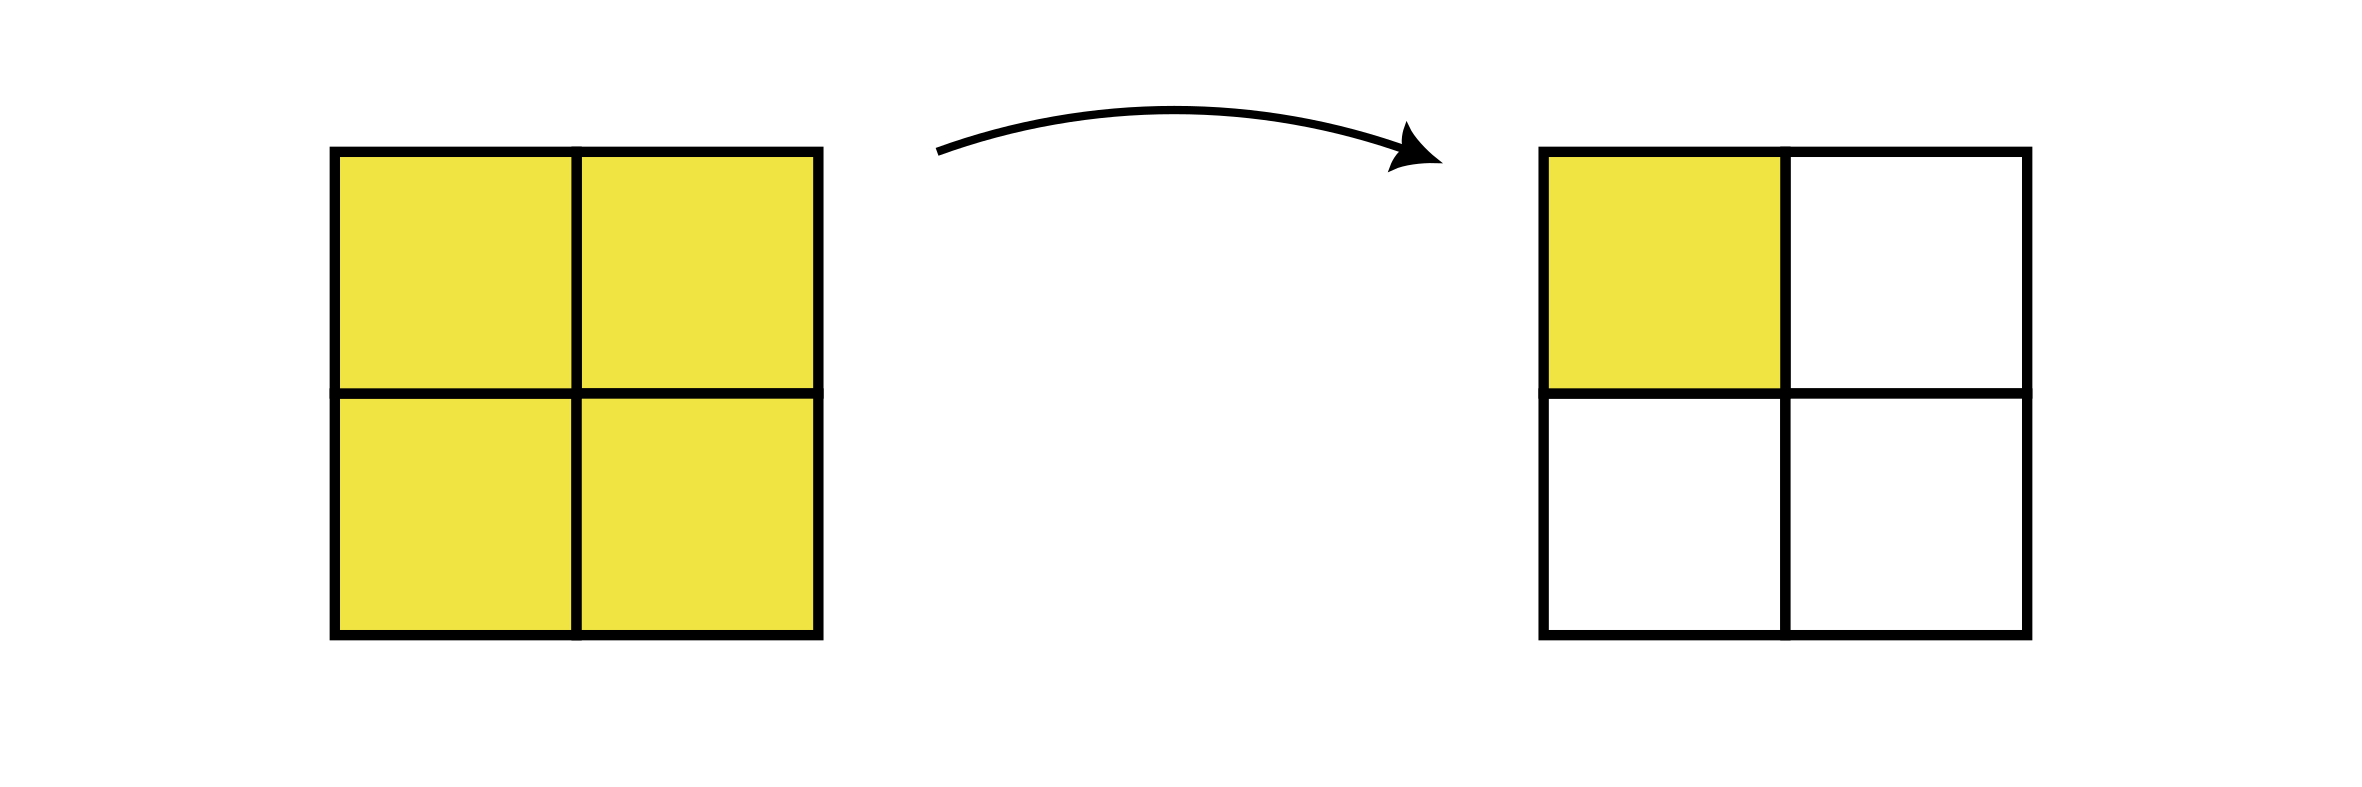
\includegraphics[width=\textwidth]{Figure 11.3.B}
\caption{An average of $3/4$ cells rotating}
\end{figure}
\noindent
then we get cell-wise expected Hamiltonians of $\frac{3}{4}$ and total system Hamiltonian Hamiltonian of $4 \cdot \frac{3}{4}$. If no rotations occur, then the Hamiltonian of the system is $0$.

The cell-wise expected Hamiltonian counts the average cumulative rotation that a cell experienced from time $t=0$ to time $t=1$. It is worth noting that rotations correspond to bit flips that only occur in even pairs for Boolean random walks. If stochastic matrix $P_{\theta \time \theta}$ has $\theta = {N \choose k}$ states, then the total system Hamiltonian between any two specific states is from the set:
$$\{0, 2, 4 ,..., 2 \cdot \min(k, N-k) \}$$
for a Boolean random walk since particles and antiparticles trade positions. The average system Hamiltonian for a state $X_0$ is the probability weighted sum of system Hamiltonians between $X_0$ and possible future state for $X_1$.

We will need to consider the define the change in energy $\Delta H$ using the $\hat \eta$ matrix defined in \textit{\S 9.5 Issues in Defining Energy}:
$$\hat \eta = 
\begin{bmatrix}
\hat \eta_{(1,1)} & \cdots & \hat \eta_{(1,\theta)} \\
\vdots & & \vdots \\
\hat \eta_{(\theta,1)} & \cdots & \hat \eta_{(\theta,\theta)}
\end{bmatrix}
$$
$$\hat \eta = \ln(\mathcal X \otimes \mathcal X) / (\pi i)$$
in which $\hat \eta_{(i,j)} = \frac{\hat X_j}{\hat X_i} = X_j \cdot X_i$. Since it matters which our initial state is when we calculate $\Delta \hat H$, we can calculate our probability distribution as:
$$\Delta H_t = I \cdot P^t (P \odot \hat \eta)$$
Let us think carefully about what this means. The identity matrix $I$ represents all possible initial states, and $P^t$ represents the time advancement from those states. The rotation from time $t$ to $t+1$ is measured by the Hadamard product $P \odot \hat \eta$.

If we are trying to calculate $\mathrm{E}(\beta_t)$, we may define $\mathrm{E}_x(\cdot)$ to refer to cell-wise expectations and $\mathrm{E}_X(\cdot)$ to refer to system-wide expectations. Considering what we know about the incomputability of Boolean mechanical systems, we might need simpler $3 \times 3$ approximations of inverse temperature for each cell. Defining a continuous definition for thermodynamic beta will be quite a bit tougher.

\section{Boolean Heat Equation}
Suppose that we wish to define a \textbf{Boolean heat equation}\index{Boolean heat equation}. The time evolution of our Boolean random walk's heat equation is given by $e^{\frac{\partial}{\partial t}} = 1 + \Delta_t$ in which:
$$\Delta_t f(x, t) = \sum\limits_{i=-d}^{d} \chi_i \Delta_{x_i} f(x,t)$$
The chording function $\chi$ gives a permissive-exhaustive chording that is a subset of all $2\cdot d$ directional differences, $2 d$ being the number of faces of each $d$-cube. Notice that $\Delta_{x_0}$ necessarily produces a difference of $0$. As discussed in \textit{7.7 n-Flip Chording and Orders} that we may consider the chording function $\chi$ to sample from the difference graph $\Delta_x X_t$ an independent set whose $2$-walks cover the difference graph $\Delta_x X_t$.

The chording function $\chi$ is actually the probabilistic Hamiltonian for each face of a cell $(x,t)$ since:
$$\chi_i \in \{0, 1\} = \ln(\{+1, -1\}) \cdot \frac{1}{\pi i}$$
This is similar to how we defined the Hamiltonian between a state $X_t$ and $X_{t+1}$, but we are reallocating the probabilities across the $2 d$ faces of each $d$-cubic cell. Any realized chording ends up double counting the number of switches due to being assigned to each cell involved in a switch.

When we define the Hamiltonian $H$ throughout most of the book, we are referring to the geometric Hamiltonian that generates the probabilities of the stochastic matrix $P = e^{\hat H \pi i}$. In this chapter, we will be using the arithmetic Hamiltonian $\bar H$ and denote it using the relation $e^{\hat H \pi i} = 1+\bar H$. In physics, the Hamiltonian operator is meant to generate time differentials of a wave function.

The Hamiltonian operator $\bar H$ is the sum of the kinetic energy operator $\bar T$ and the potential energy operator $\bar V$:
$$\Delta_t f(x, t) = \sum\limits_{i=-d}^{d} \chi_i \Delta_{x_i} f(x,t)$$
$$ = \sum\limits_{i=-d}^{d} \bar H f$$
$$ = \sum\limits_{i=-d}^{d} (\bar T + \bar V) f$$
We are not obligated to define the Hamiltonian operator in the same way as quantum mechanics necessarily. What are the kinetic and potential energy operators exactly? How should we define them? 

It really depends on our convention. Do we imagine particles as having a fixed kinetic energy and the stochastic potential energy function closing off other bit flips? Do we imagine particles as having a fixed potential and the stochastic kinetic energy function balancing out accumulation of probabilities? 

Here is a list of our possible conventions for Boolean random walks:
\begin{enumerate}
\item Stationary: A Boolean random walk field has no kinetic energy $\bar T = 0$, thus $\bar H = \bar V$.
\item Kinetic-Electric: A Boolean random walker has kinetic energy, thus $\bar T = (T_{-d},...,T_0,...,T_{d})$ in which $T_d \propto \Delta_x f$. We then define $\bar V = \bar H - \bar T$.
\item Potential-Electric: A Boolean random field is an potential energy field, thus $\bar V = (V_{-d},...,V_0,...,V_{d})$ in which $V_d \propto \Delta_x f$. We then define $\bar T = \bar H - \bar V$.
\item Bound Energy: The differences dictate energy levels $H_d \propto \Delta_x f$, thus kinetic energy $T$ is the maximal independent set and $V$ is the unused energy.
\end{enumerate}
We shall use the kinetic convention as that is the one that makes the most sense for Boolean random walks. The kinetic operator $\bar T$ produces a sort of pseudo-Laplace operator since we are performing a first-order finite difference across all $2 d$ faces of the $d$-cubic cell. 

Consider the Hamiltonian $H$ of the Schr\"{o}dinger equation of quantum mechanics. The Hamiltonian operator $H$ generates time differences like so:
$$H = i \hbar \frac{d}{dt}$$
If we decompose $H$ into its kinetic energy $T$ and potential energy $V$ components, we get:
$$\hat H = \hat T = \hat V$$
$$\iff \hat H = -\frac{\hbar^2}{2m} \nabla \cdot \nabla + V(x, t)$$
The kinetic energy term $\hat T$ is the Laplacian $\nabla \cdot \nabla$ and the potential energy term is often used to refer to some sort of environmental influence such as a magnetic field. The kinetic convention is the one that makes the most sense due to its structural similarity to the heat equation and the Schr\"{o}dinger equation.

The stationary convention is useful for a cellular automaton because energy lacks a sensible meaning for something like Conway's \textit{Life}. The ideas of momentum and kinetic energy do not transfer well in the definition of a cellular automaton in general. We only need to define local transition probabilities. Performing a Fourier transform to derive ``momentum'' from some general transition function has no simple interpretation . 

The bound energy convention is incorrect the Hamiltonian $H$ does not generate time differences in our heat equation at all. This is perhaps the one that makes sense in the context of physical systems in which stored energy is potential energy. It also gives nonsensical notions of temperature since the difference structure of $H = \Delta_x f$ changes dramatically at the system and cellular level.

We define $\bar H = (H_{-d},...,H_0,...,H_d)$ to be the Hamiltonian across each face of a $d$-cubic cell, $\bar T = (T_{-d},...,T_0,...,T_d)$ to be the kinetic energy across each face, and $\bar V = (V_{-d},...,V_0,...,V_{d})$ to be the potential energy across each face. We may like $H_0$ to represent null bit flips, but this is definitely an improper representation. The dot product $1 \cdot \bar H$ gives the average bit rate of the cell.

We use the kinetic convention, which is the implicit rule that makes the most sense when determining maximal independent sets. The potential operator $\bar V$ ``counters'' the kinetic operator $\bar T$, what would be a good intuition for $\bar V$? We might consider it to be the magnetic vector potential that results in inductance, opposing chances to the electric flow.

If we set $\hat T = |\Delta_x f|$ in which $f \in \{0, 1\}$, then we get:
$$\Delta_t f(x, t) = \sum\limits_{i=-d}^{d} \chi_i \Delta_{x_i} f(x,t)$$
$$ = \sum\limits_{i=-d}^{d} \bar H f$$
$$ = \sum\limits_{i=-d}^{d} (\bar T + \bar V) f = \sum\limits_{i=-d}^{d} (\Delta_x + \bar V) f $$
The kinetic operator $\bar T$ produces a sort of pseudo-Laplace operator since we are performing a first-order finite difference across all $2 d$ faces of the $d$-cubic cell. As a reminder, the end result is that a random transition for $\bar H$ is given by maximal independent sets.


If $|\Delta|$ is a function that produces produces $1$ if there is a difference and $0$ if there is no difference, then $\mathbb B_\circ = \{0, 1\}$ allows us to denote:
$$\chi = \chi^C \oplus |\Delta| \iff \bar H = \bar T + \bar V$$
in which $\oplus$ is the \textbf{XOR} operator, also known as the Boolean symmetric difference operator. The chording set function $\chi$ has a complement chording set function of $\chi^C = |\Delta| \oplus \chi$. Due to the way that \textbf{XOR} is defined, we have no need for positive or negative energy.

A physical system seeks to minimize its potential energy, and it does this by seeking a local minimum in the potential energy function $V(x)$:
\begin{figure}[H]
\centering
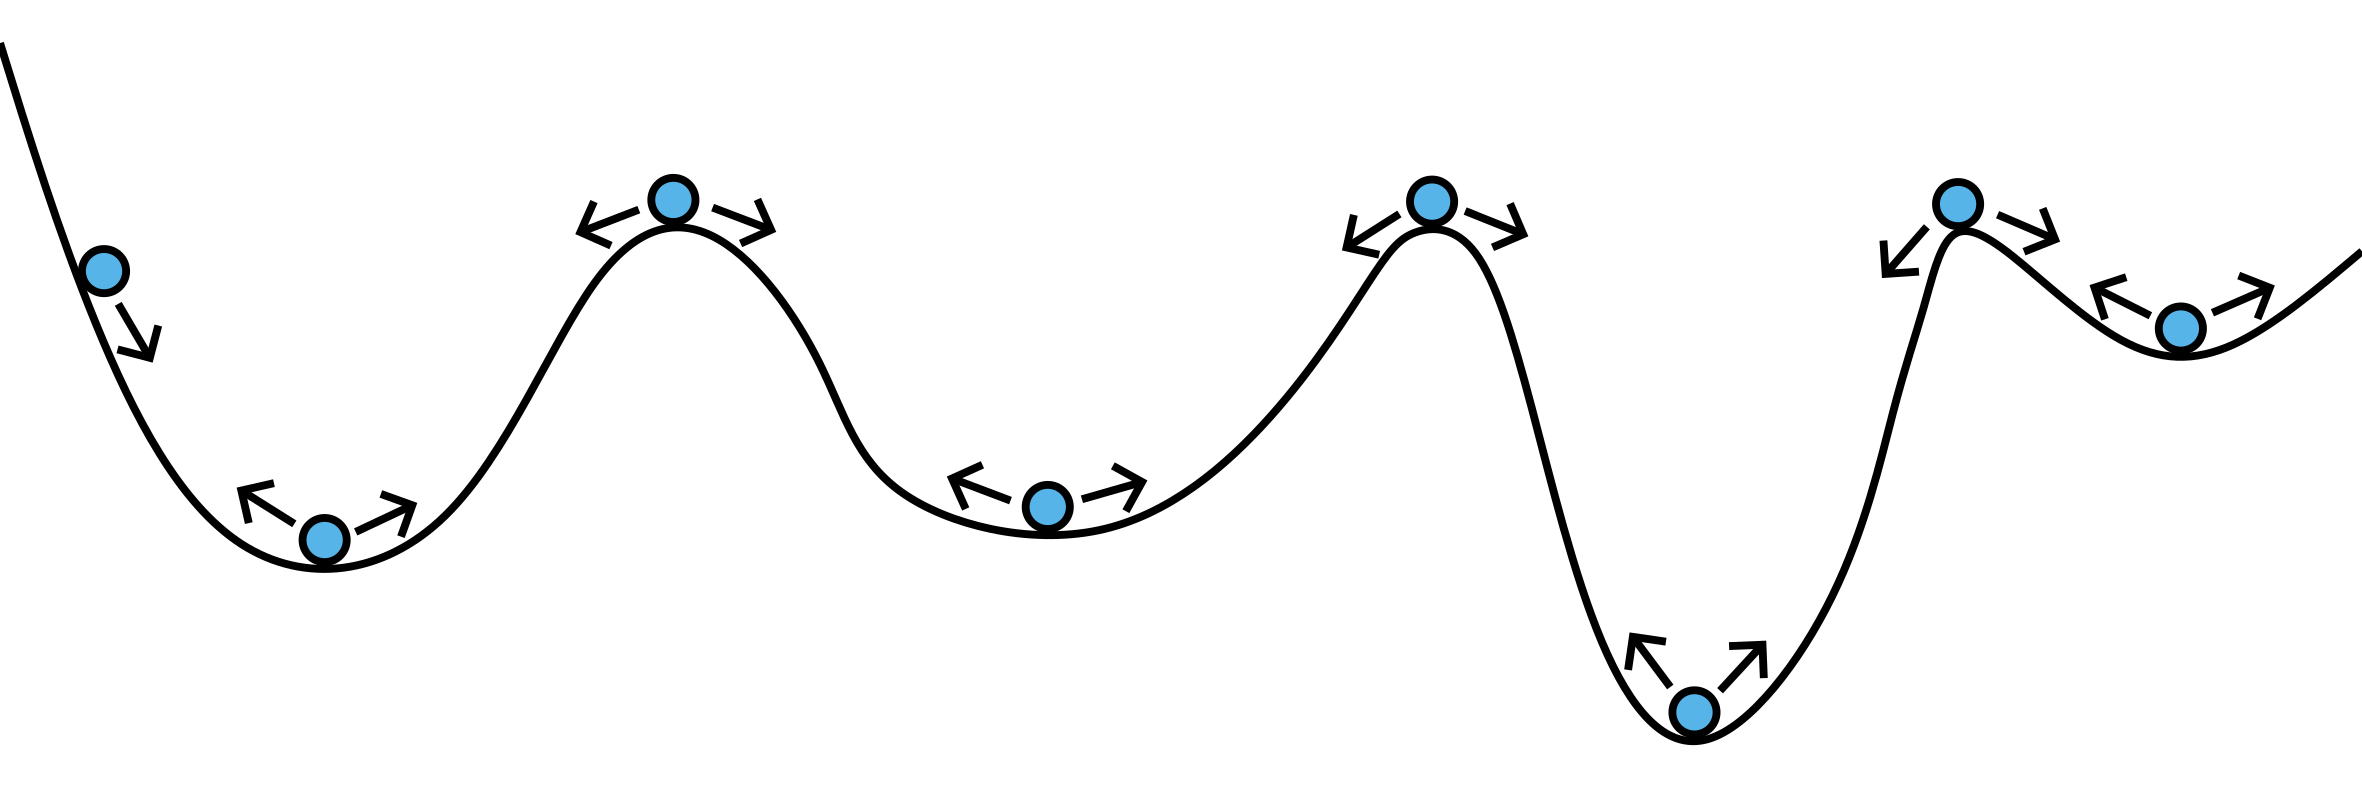
\includegraphics[width=\textwidth]{Figure 11.4.A}
\caption{Balls tend to roll down a potential well}
\end{figure} \noindent
\noindent % An image of balls rolling down a potential well
It means that a physical system resists increases to potential energy and attracts attention to actions that decrease potential energy. The equivalent of this in Boolean statistical mechanics are the eigenvectors of a transition matrix $P$. The transition rule that we apply to individual cells determines the shape of the geometric potential upon a simplex.


A Boolean random walk likewise seeks to minimize its unused potential energy $\hat V$ by preferring one of the maximal independent sets that is a maximum independent set. This is identical to the discussion of choosing a minimal dominating set or maximal independent set for a Boolean random walk:
\begin{figure}[H]
\centering
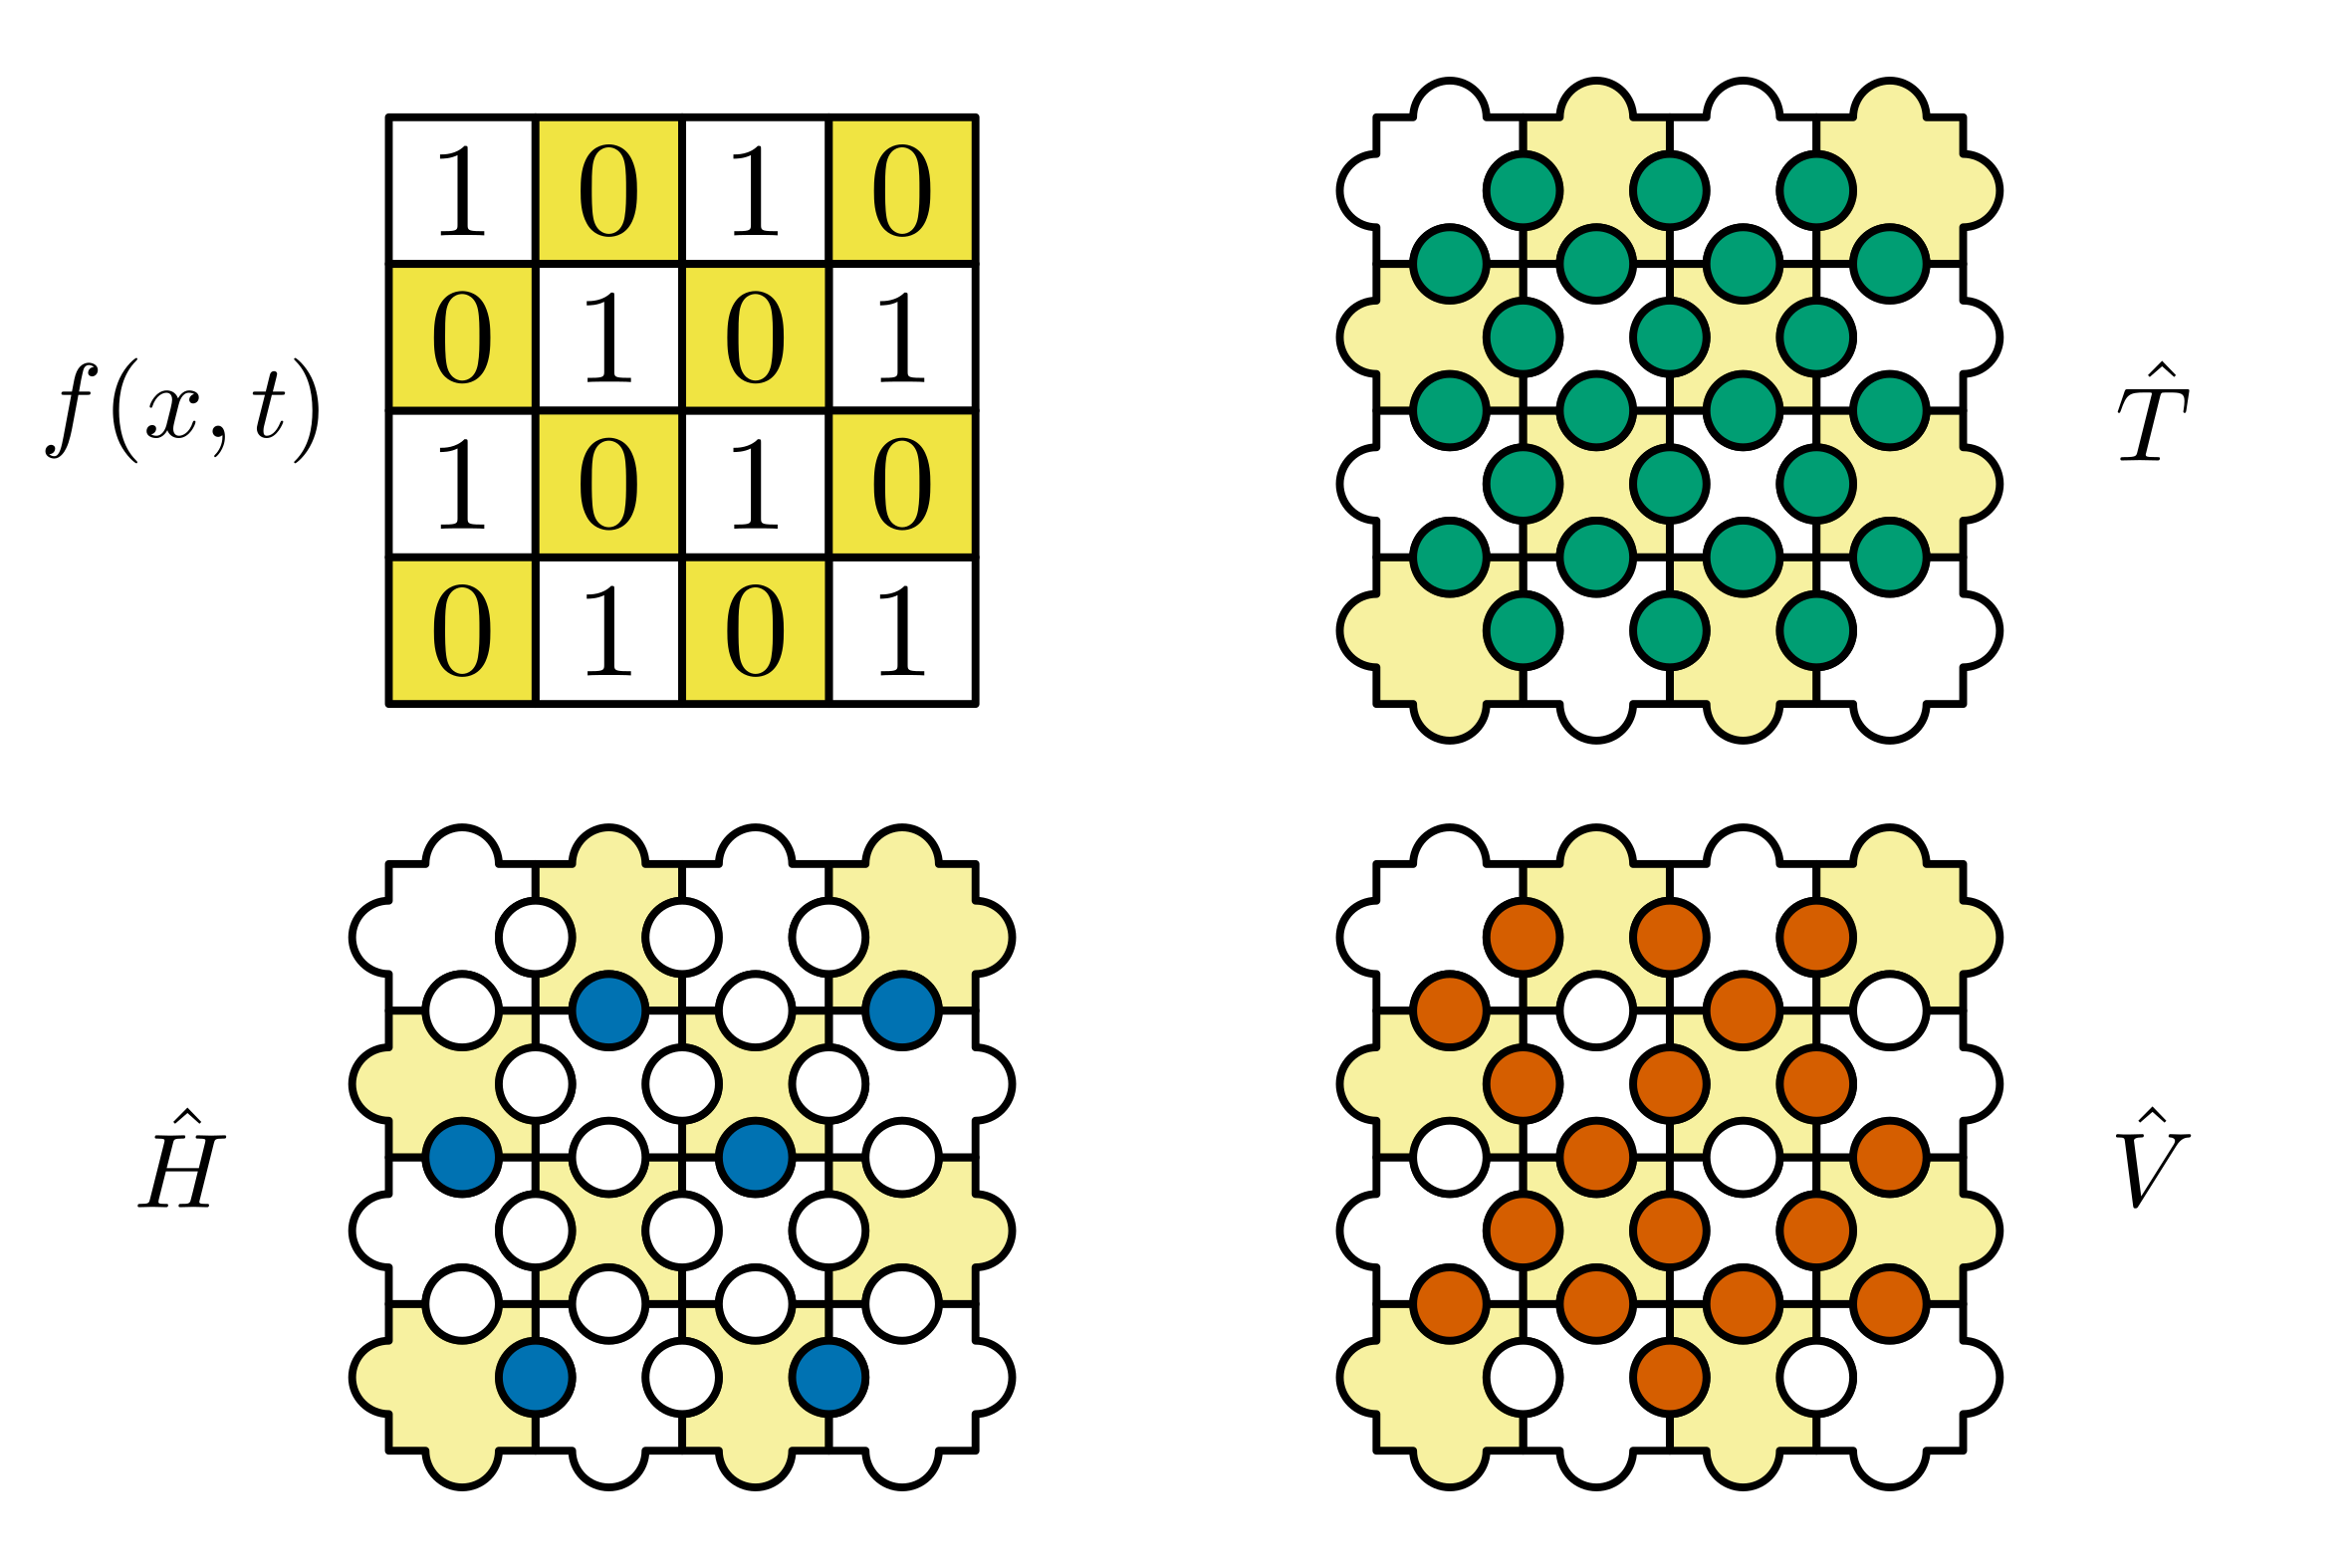
\includegraphics[width=\textwidth]{Figure 11.4.B}
\caption{Underutilized potentials $V$ indicate less likely transitions for $H$}
\end{figure} \noindent
\noindent % A planar and an underutilized transition
In this example, a maximal independent set that is not some maximum independent set is less likely. Under the kinetic convention, more unused faces results in a higher potential energy. As a Markov chain, this unused potential energy includes unused states in the state space. Just like in physics, this would mean that the field resists ``wasting'' unused potential energy.

If we are going with the kinetic convention, we might consider the \textbf{Ehrenfest theorem}\index{Ehrenfest theorem} when attempting to find some way the potential function changes with time. Since our convention is to use $a$ instead of $p$ for momentum:
$$\frac{d}{dt} \langle x \rangle = \langle a \rangle, \frac{d}{d t} \langle a \rangle = \langle \frac{d}{dx} V(x) \rangle$$
If we adapt this definition to Boolean statistical mechanics, we can use the definition of the Hamiltonian as $\frac{\partial}{\partial t} = 2 \pi i \eta$:
$$(\frac{\partial}{\partial t})^2 \langle X \rangle = \langle \frac{d}{dx} V(x) \rangle$$
$$ (\pi i \eta) \langle X \rangle = \langle \frac{d}{dx} V(x) \rangle$$
We need to remap and adapt this definition to work with our heat equation on cubic lattices and our understanding of stochastic transition matrices:
$$ (\pi i \eta) \langle X \rangle = \langle (\nabla \cdot \nabla) V(x) \rangle$$
$$ - \pi^2 \eta^2 \Phi X \Phi^{-1} = \Phi (\nabla \cdot \nabla) V(x) \Phi^{-1}$$
Perhaps we will need to move the values inside the expectation operator $\langle \ \cdot \ \rangle$:
$$- \Phi \pi^2 \eta^2 X \Phi^{-1} = \Phi (\nabla \cdot \nabla) V(x) \Phi^{-1}$$
Now we can undo the expectation and solve for $V(x)$:
$$ - (\nabla \cdot \nabla)^{-1} \pi^2 \eta^2 X = V(x)$$
This is a non-rigorous interpretation and likely incorrect derivation of analytic potential energy. It is at ltast a worthwhile baseline to compare for a future researcher to properly derive a definition in the future.

The inverse of the Laplace operator is probably not well-defined for lattice mechanics, especially if we are use the pseudo-Laplace definition of:
$$\nabla \cdot \nabla \approx \sum\limits_{k=-d}^d \Delta_k$$
The inverse Laplacian of $X$ is somewhat inaccurate because we should be operating on the harmonic eigenstates $X = \hat A(x)$ since it as if we ``inside'' the expectation. The inverse-Laplacian acts \textit{non-locally} since it depends on an integral that acts upon all points in space. We are likely better of simply estimating the potential energy $V$ for a specific starting state $X_0$.

Thermodynamic systems tend to maximize entropy as they diverge from a known state, denoted as entropy $0$. Likewise, they seek to minimize potential energy (average or total) by approaching the stationary distribution. We may possibly observe a Boolean mechanical system to have a macroparticle if the local change in potential energy is approximately $0$.


\section{Boolean Thermodynamics}
The \textbf{coldness}\index{coldness} $\beta$, also known as \textbf{thermodynamic beta}\index{thermodynamic beta}, measures the change in the entropy with respect to the energy. The formula in physics is:
$$\beta = \frac{\partial S}{\partial E}$$
in which $S$ is the entropy and $E$ is the energy. The simplest adaptation we can use for Boolean statistical mechanics is to consider coldness from the perspective of a known state using the forward difference operator:
$$\frac{\Delta S}{\Delta H} = \frac{-P \odot \ln(P)+0}{\ln[X_1 / X_0] / \pi i} $$
This however, defines distribution coldness $\alpha$ instead of a more familiar definition of coldness $\beta$ such that a system's temperature can increase or decrease as it changes from one configuration to another due to some event.\footnote{By configuration, we mean microstate in the statistical mechanics sense.} We need to be careful what we mean by temperature and coldness.

Observe the following evolution:
\begin{figure}[H]
\centering
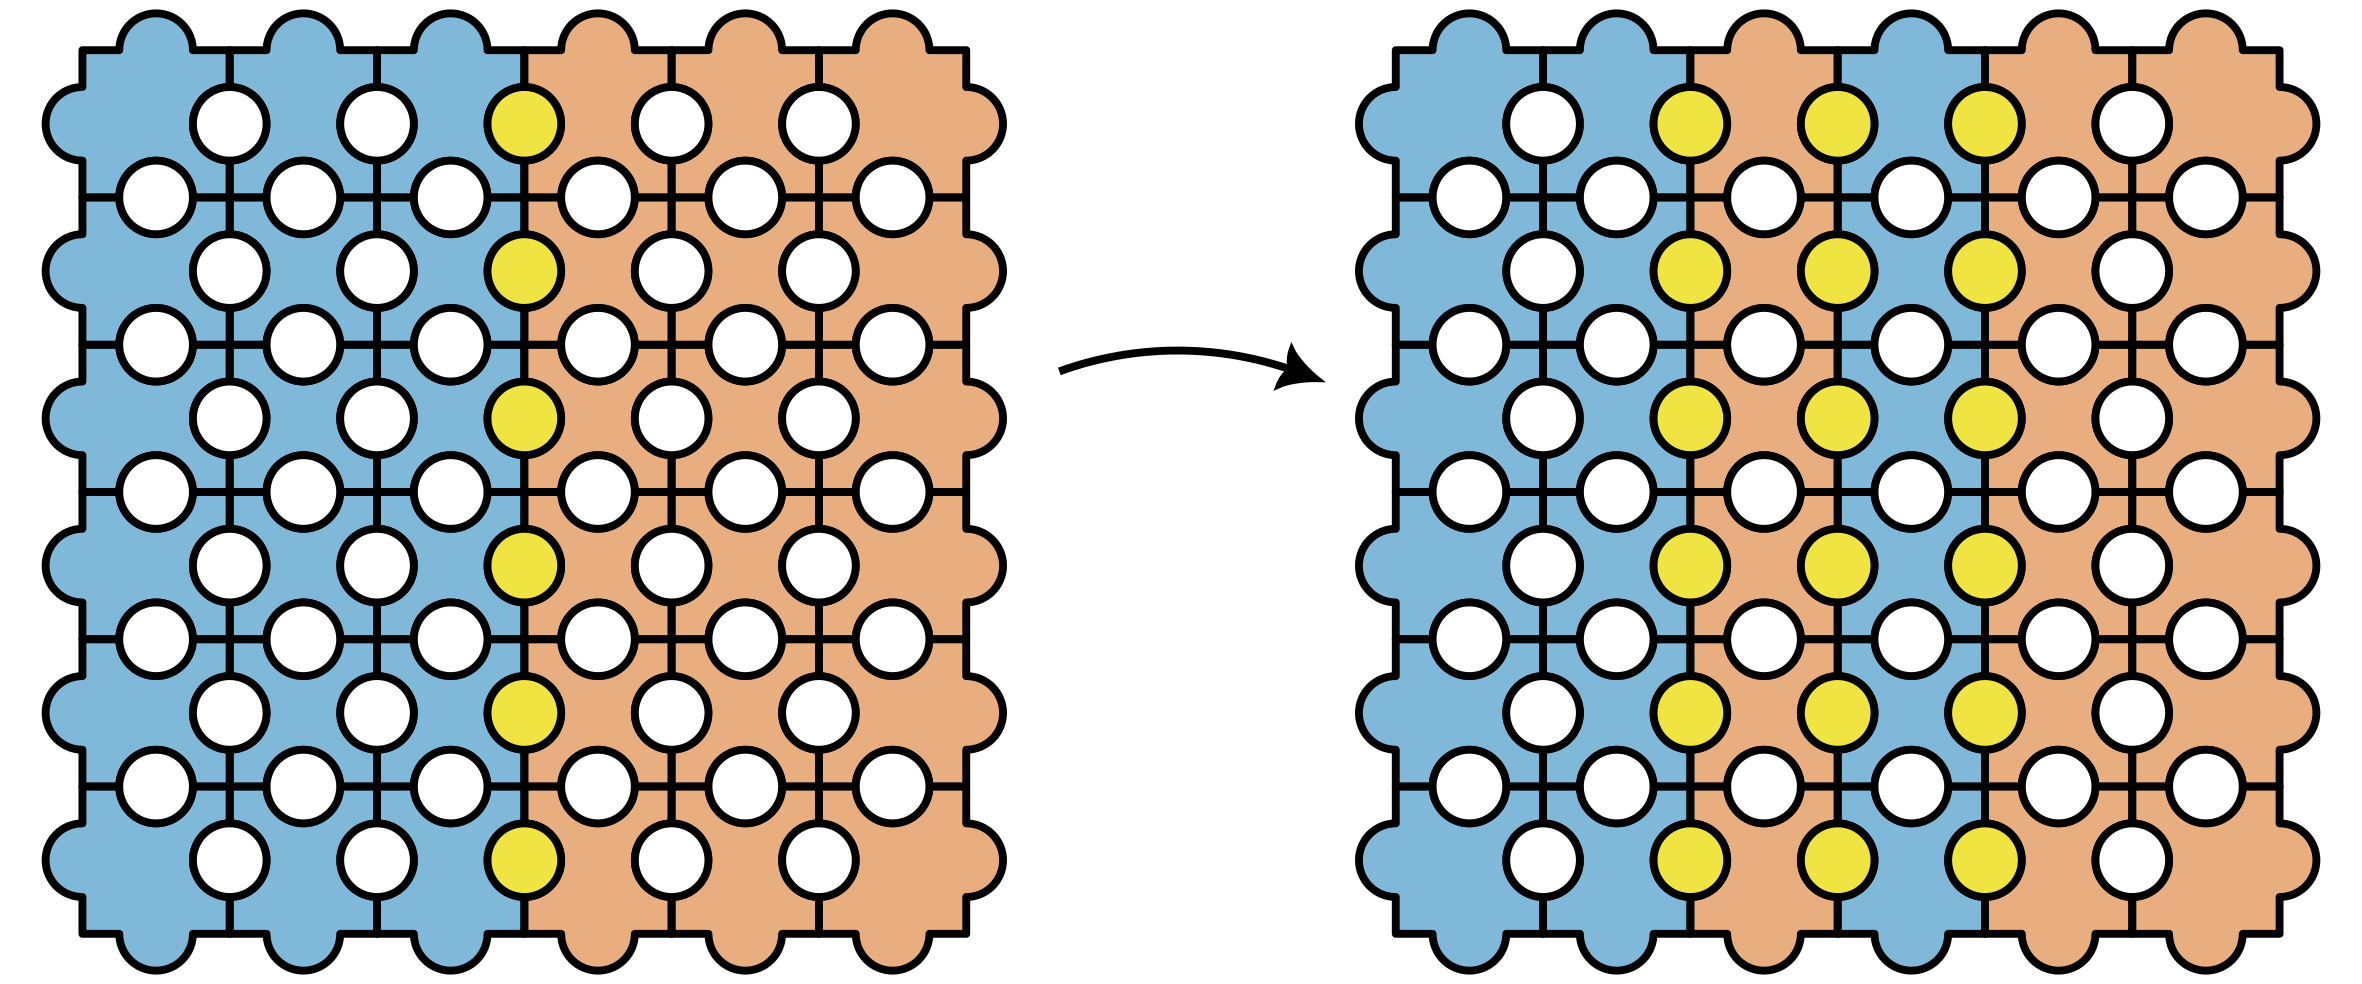
\includegraphics[width=\textwidth]{Figure 11.5.A}
\caption{A $6 \times 6$ planar state increasing in temperature}
\end{figure} \noindent
\noindent % An image of a 6x6 planar state evolving deterministically:
A relatively small change in the phase of the system's cells has dramatically increased its entropy. After one time step, the entropy of the cells that changed has gone from 0 to 1 shannon or bit: pairs may go further or reverse the exchange. It should not matter if the system is majority particles of majority antiparticles. Thermodynamic beta $\beta$ should only care about how much entropy increases per unit of rotation.

If we choose a square system larger than our $6 \times 6$ example, the planar separated state is colder due to lower average change in the phase of the $\ell \times \ell$ system but the change in the entropy is proportional to $\ell$ bits or shannons:
\begin{figure}[H]
\centering
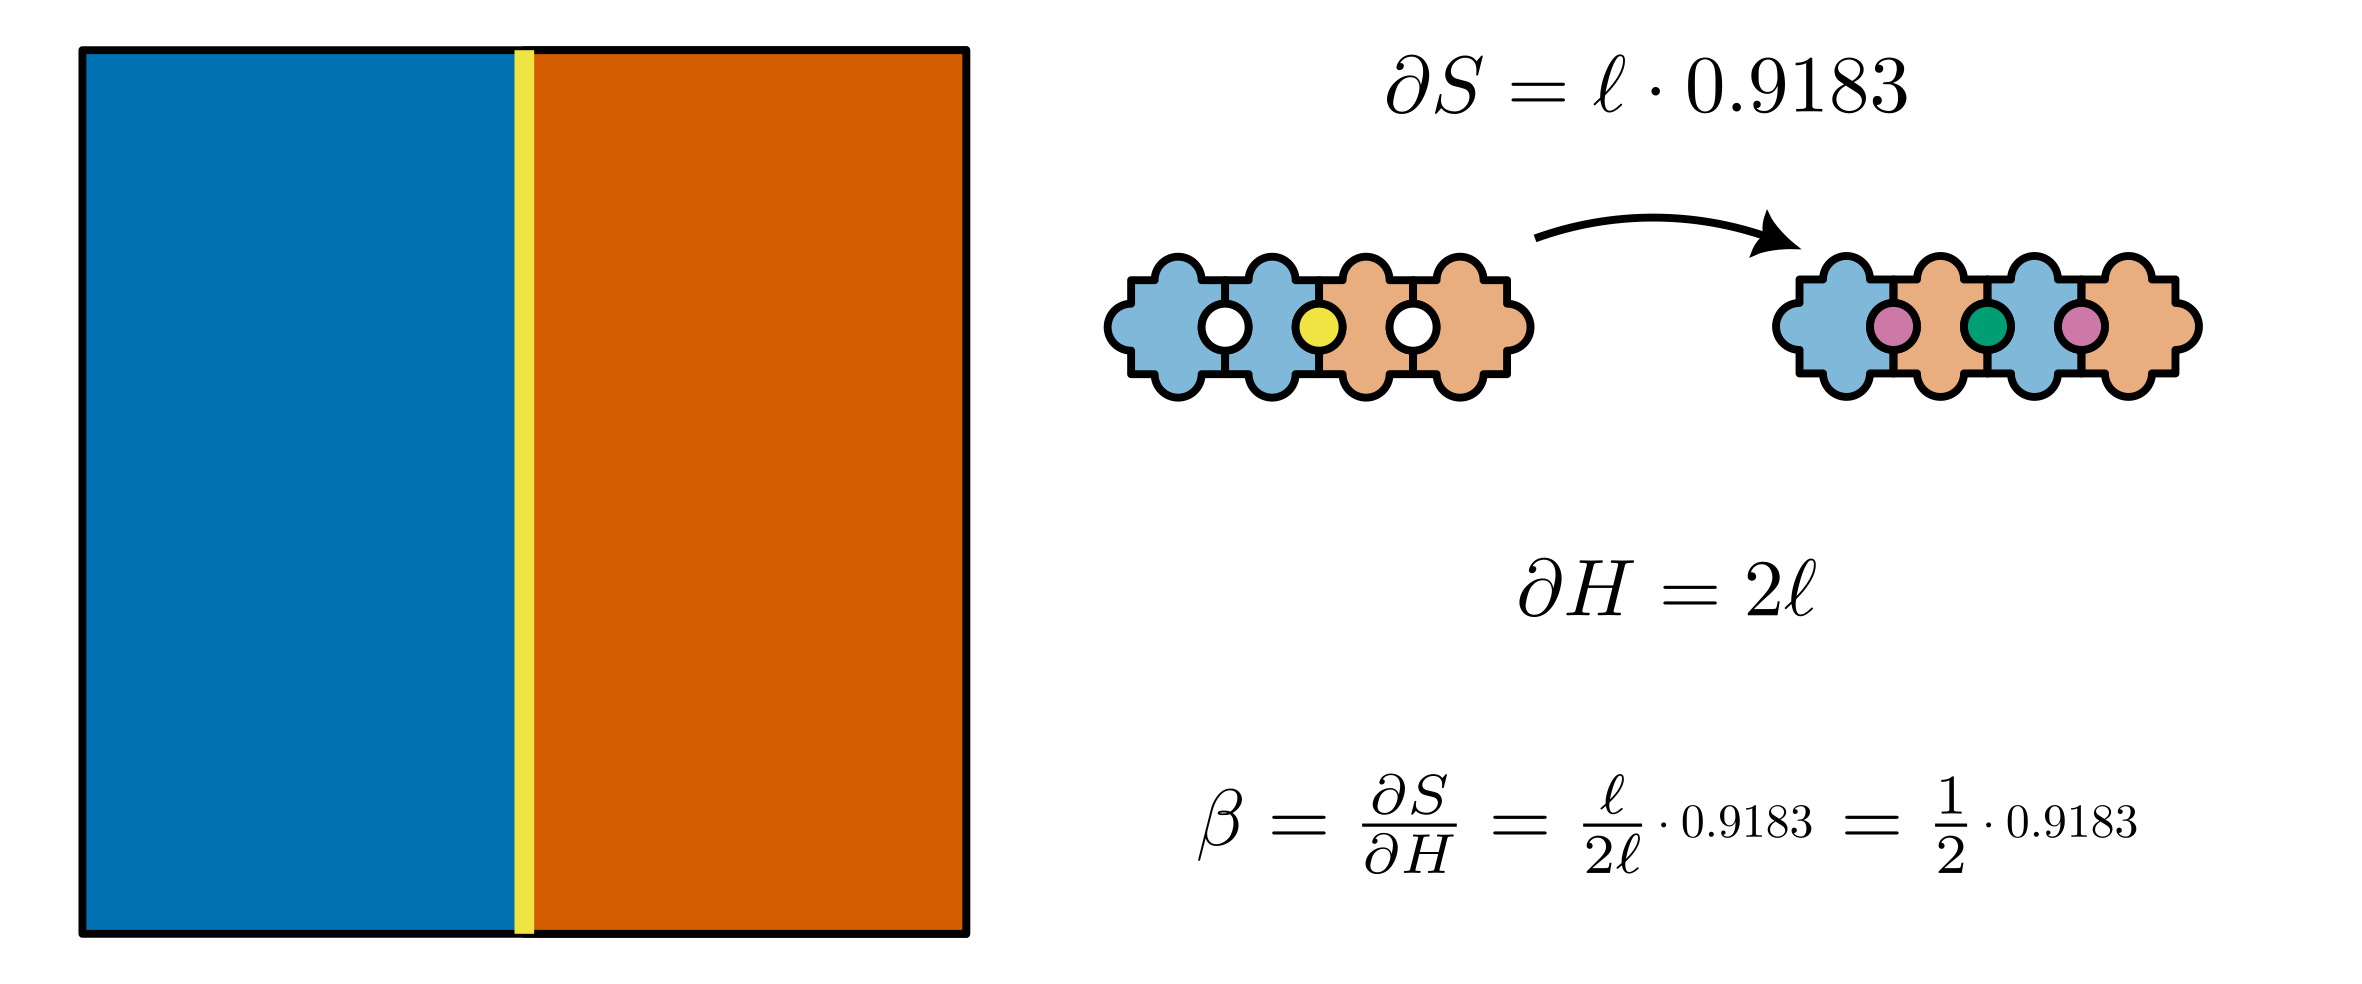
\includegraphics[width=\textwidth]{Figure 11.5.B}
\caption{The inverse temperature is approximately $\frac{1}{2} \cdot 0.9183$ regardless of length $\ell$ because the number of possible states increases from $2^0$ to $2^{\ell \cdot 0.9183}$ and the number of cells that rotated was $2 \ell$.}
\end{figure} \noindent
\noindent % An continuum representation of thermodynamic beta
The Shannon entropy of an individual row would be identical to that in \textit{Figure 9.2} for $\frac{1}{3}\log_2(\frac{1}{3}) + \frac{2}{3}\log_2(\frac{2}{3}) \approx 0.9183$. Since each row is independent, the entropy rate of the new state is $0.9183 \cdot \ell$. Since the original state only has one valid transition, the Shannon entropy is $\log_2(1)=0$. Therefore, the difference is entropy is $0.9183 \cdot \ell - 0$.

The number of cells that change is $2 \ell$, and the change in the Hamiltonian of each cell is $\frac{1}{2}$ cycles. If we choose to define energy via angles, then the coldness is $\beta = 0.9183$. If we instead define energy as the number of cells that change, then it is defined as $\beta = \frac{1}{2}\cdot 0.9183$. We should be concerned about how we handle this definition because we may sometimes deal with infinities or division by $0$.

The minimum coldness $\beta$ is achieved by considering the $2 \times 2$ oscillator:
\begin{figure}[H]
\centering
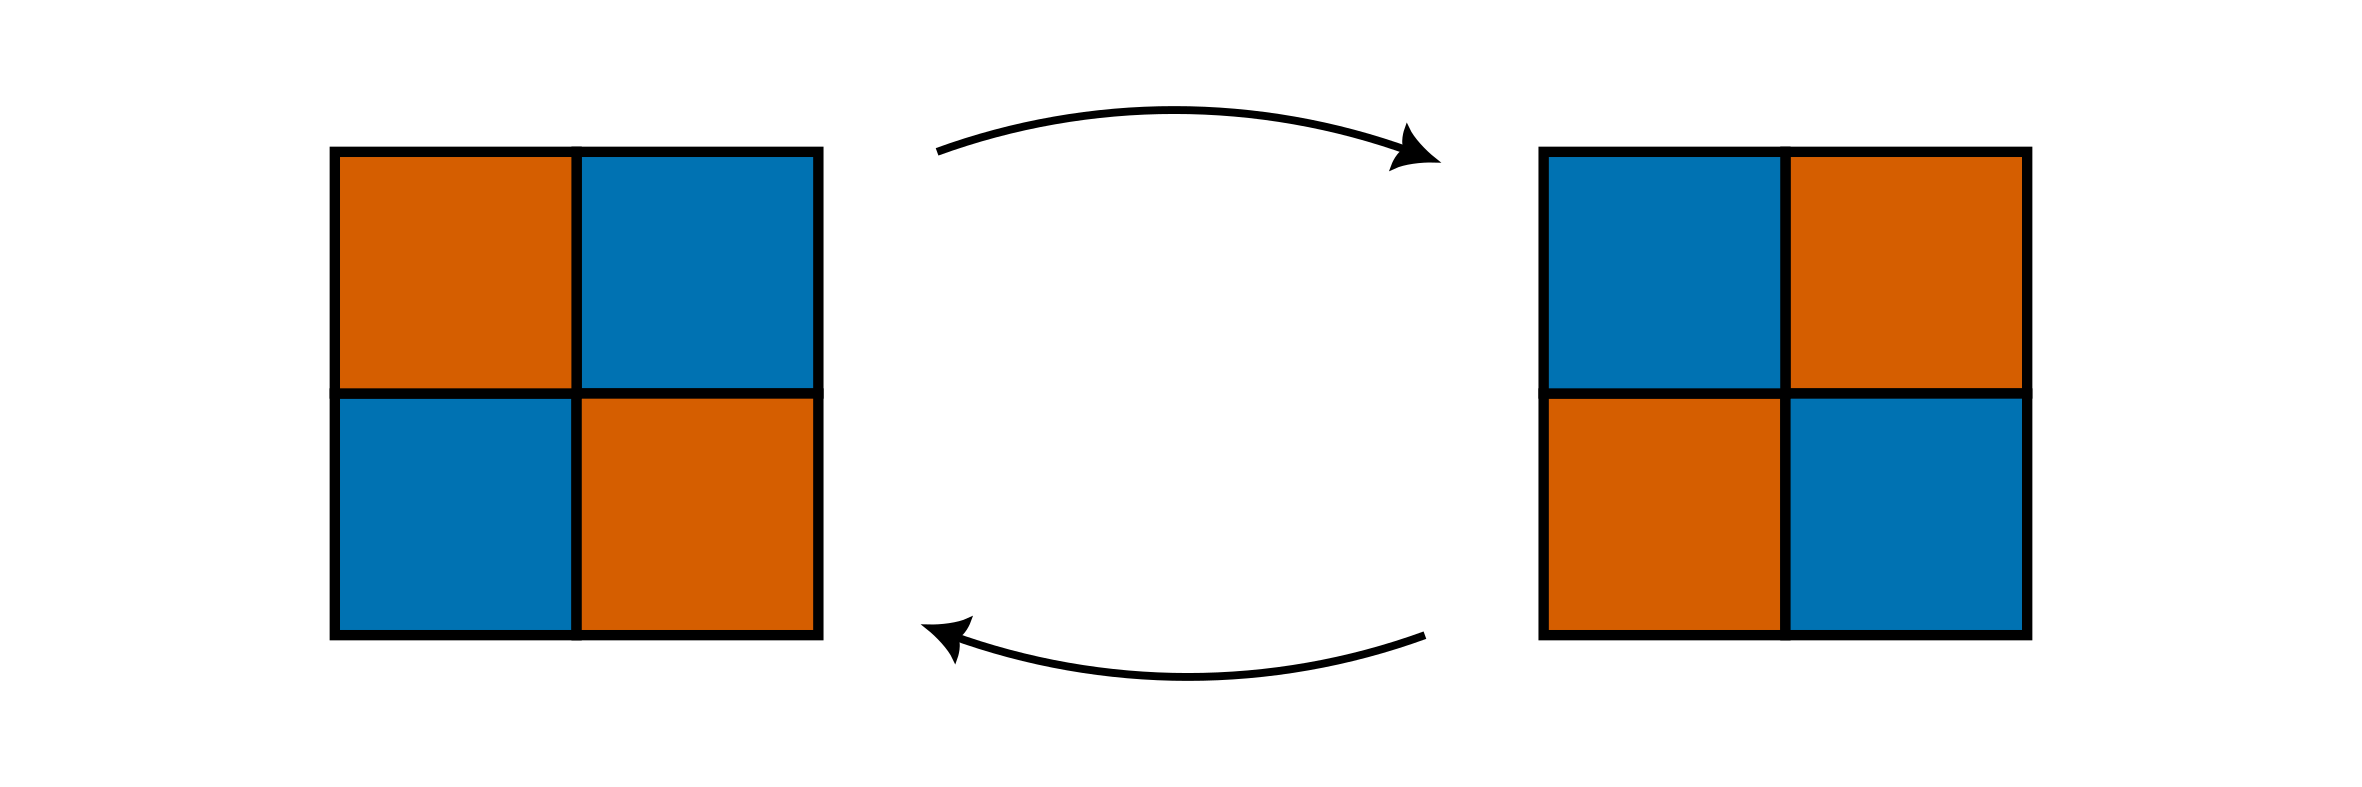
\includegraphics[width=\textwidth]{Figure 11.5.C}
\caption{The coldness should be exactly $\beta = 0$}
\end{figure} \noindent
\noindent % 2x2 Oscillator
The entropy has changed by $0$ yet every cell has changed. Since coldness $\beta$ is inverse temperature, then:
$$\beta^{-1} = T = 0^{-1} = \infty$$
The $2 \times 2$ oscillator is of infinite temperature. Alternatively the $2 \times 2$ frozen state:
\begin{figure}[H]
\centering
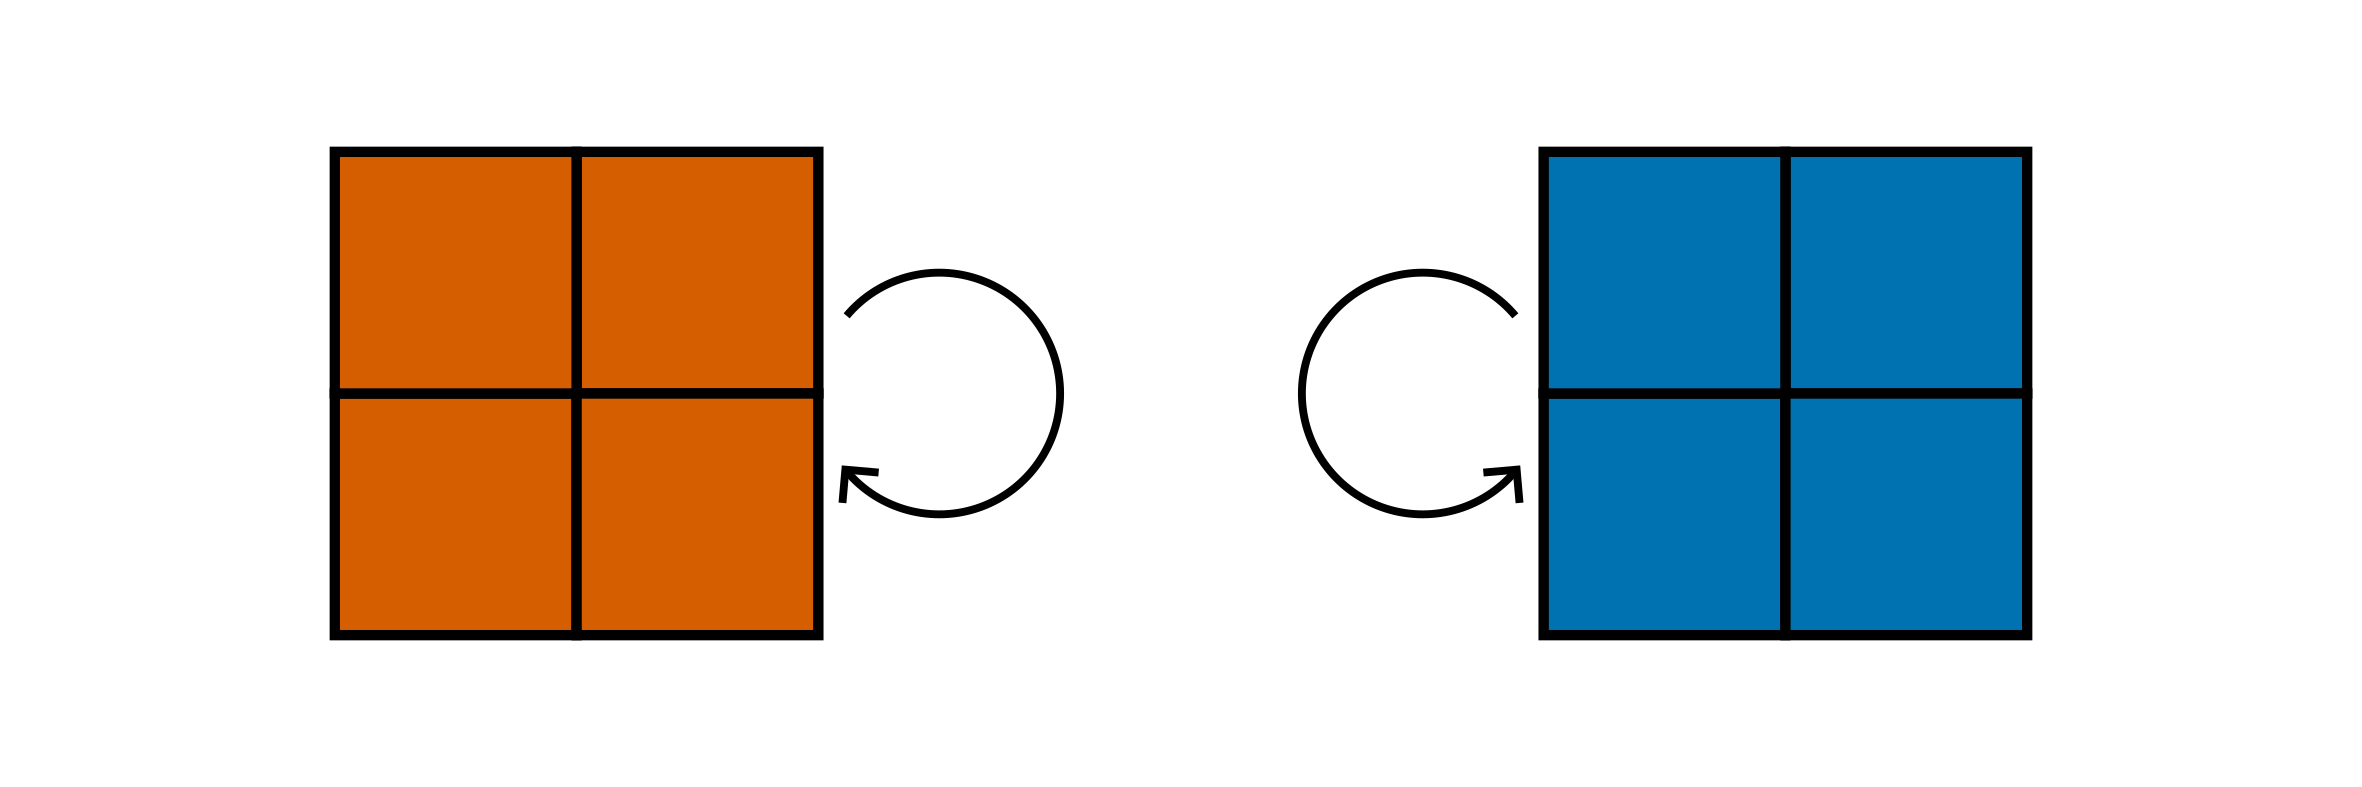
\includegraphics[width=\textwidth]{Figure 11.5.D}
\caption{The coldness $\beta = 0/0$ is undefined.}
\end{figure} \noindent
\noindent % 2x2 Still
has $0$ entropy change and $0$ cells change. One possible convention is that $0 / 0 = 1$, but this brings our inverse temperature to be the same as the planar state. Is this correct or incorrect? If we chain several planar states together like a layered cake, then the coldness is the same as a single planar state. Likewise, we observed before that extending a planar state along a new dimension preserves its coldness. If we claim that $0/0 = 0$, then we need to justify our definition for inconsistency.

We shall decide that it is generally better to determine the coldness using the Boolean ring set $\mathbb B_\circ = \{0, 1\}$ instead of the method of Hamiltonians definition $\{ 0, \frac{1}{2} \}$. This makes the coldness of the planar state have coldness $\beta = 1/2$ and the frozen still state have coldness $\beta = 1$ for Boolean random walks. We will mimic the way that we handle coldness $\beta$ when applied to matrices.

We shall refer to this method as the \textbf{geometric cellular coldness}\index{geometric cellular coldness} of a particular transition. This definition is incomplete because we have not introduced probabilistic components.

Before we define the coldness of a cell, we should generate an intuition of why coldness is a superior representation over temperature. Consider the following diagram of in which the height represents the energy that a particle contains:
\begin{figure}[H]
\centering
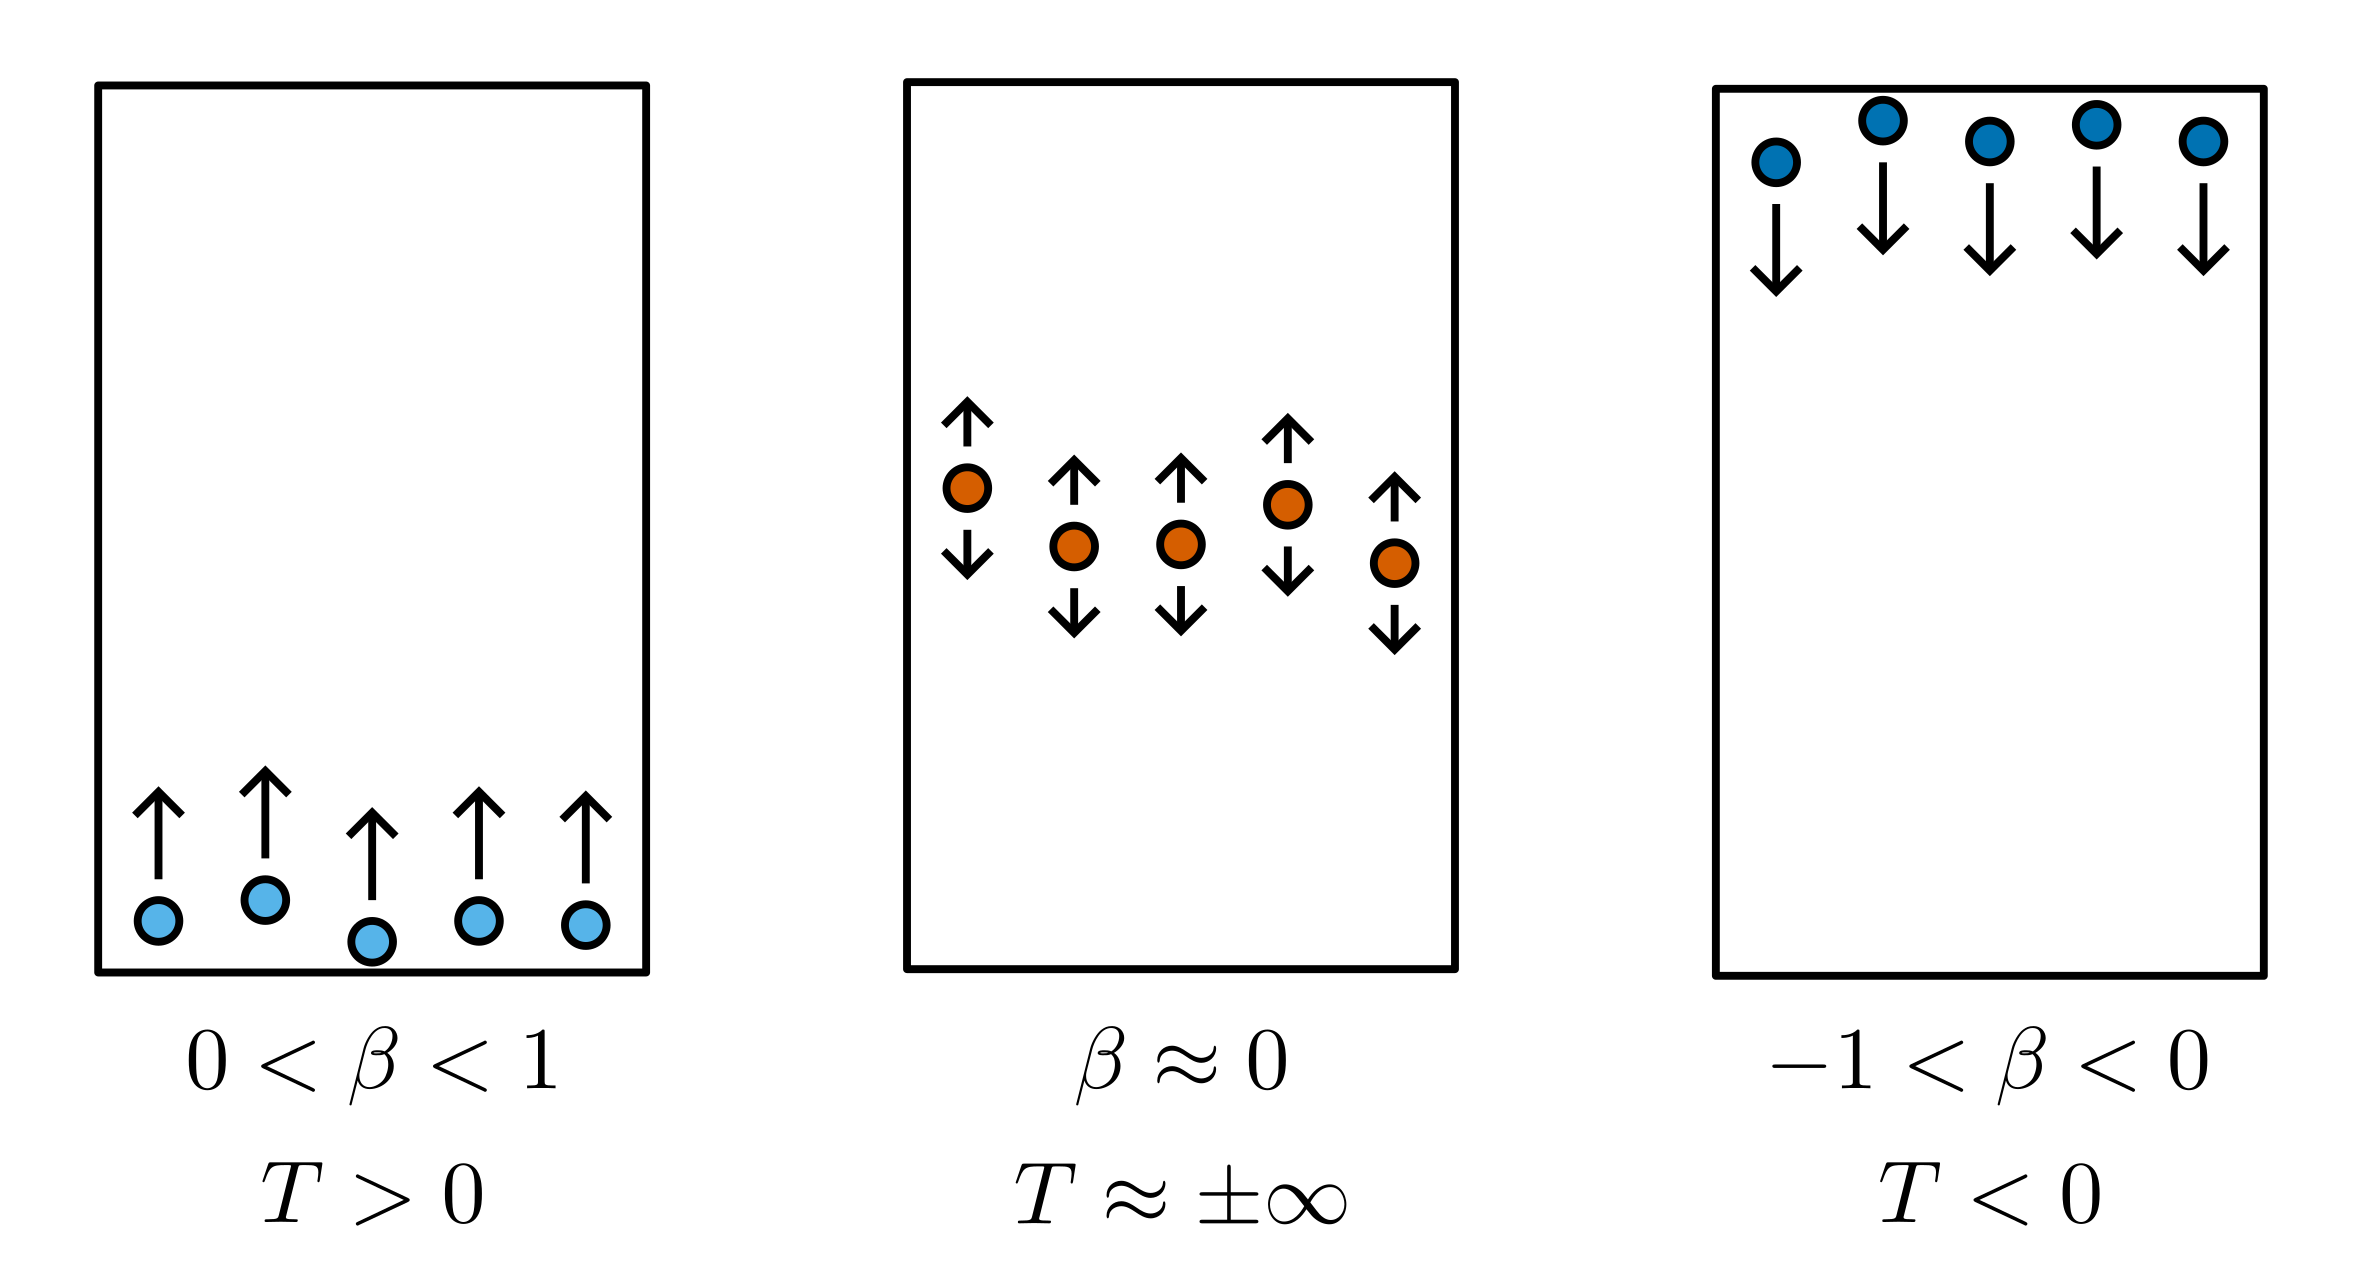
\includegraphics[width=\textwidth]{Figure 11.5.E}
\caption{Particles at various energy levels}
\end{figure} \noindent
For a particle at some initial energy level, it can jump energy levels up or down. For the left box, increasing energy will increase entropy. For the middle box, increasing energy will not increase entropy much. For the right box, increasing energy will actually decrease energy. At the coldest temperature, adding one unit of energy will increase the entropy by one unit of information, a bit.

This should give us an intuition of what we expect the coldness of a single cell to be. The coldness of a specific cell is about whether a rotation increases or decreases the entropy of a single cell, on average. In other words, does a bit flip increase the entropy of future bit flips?

The following crossing diagram can help illuminate what the \textbf{cellular coldness}\index{cellular coldness} of a cell might be interpreted as:
\begin{figure}[H]
\centering
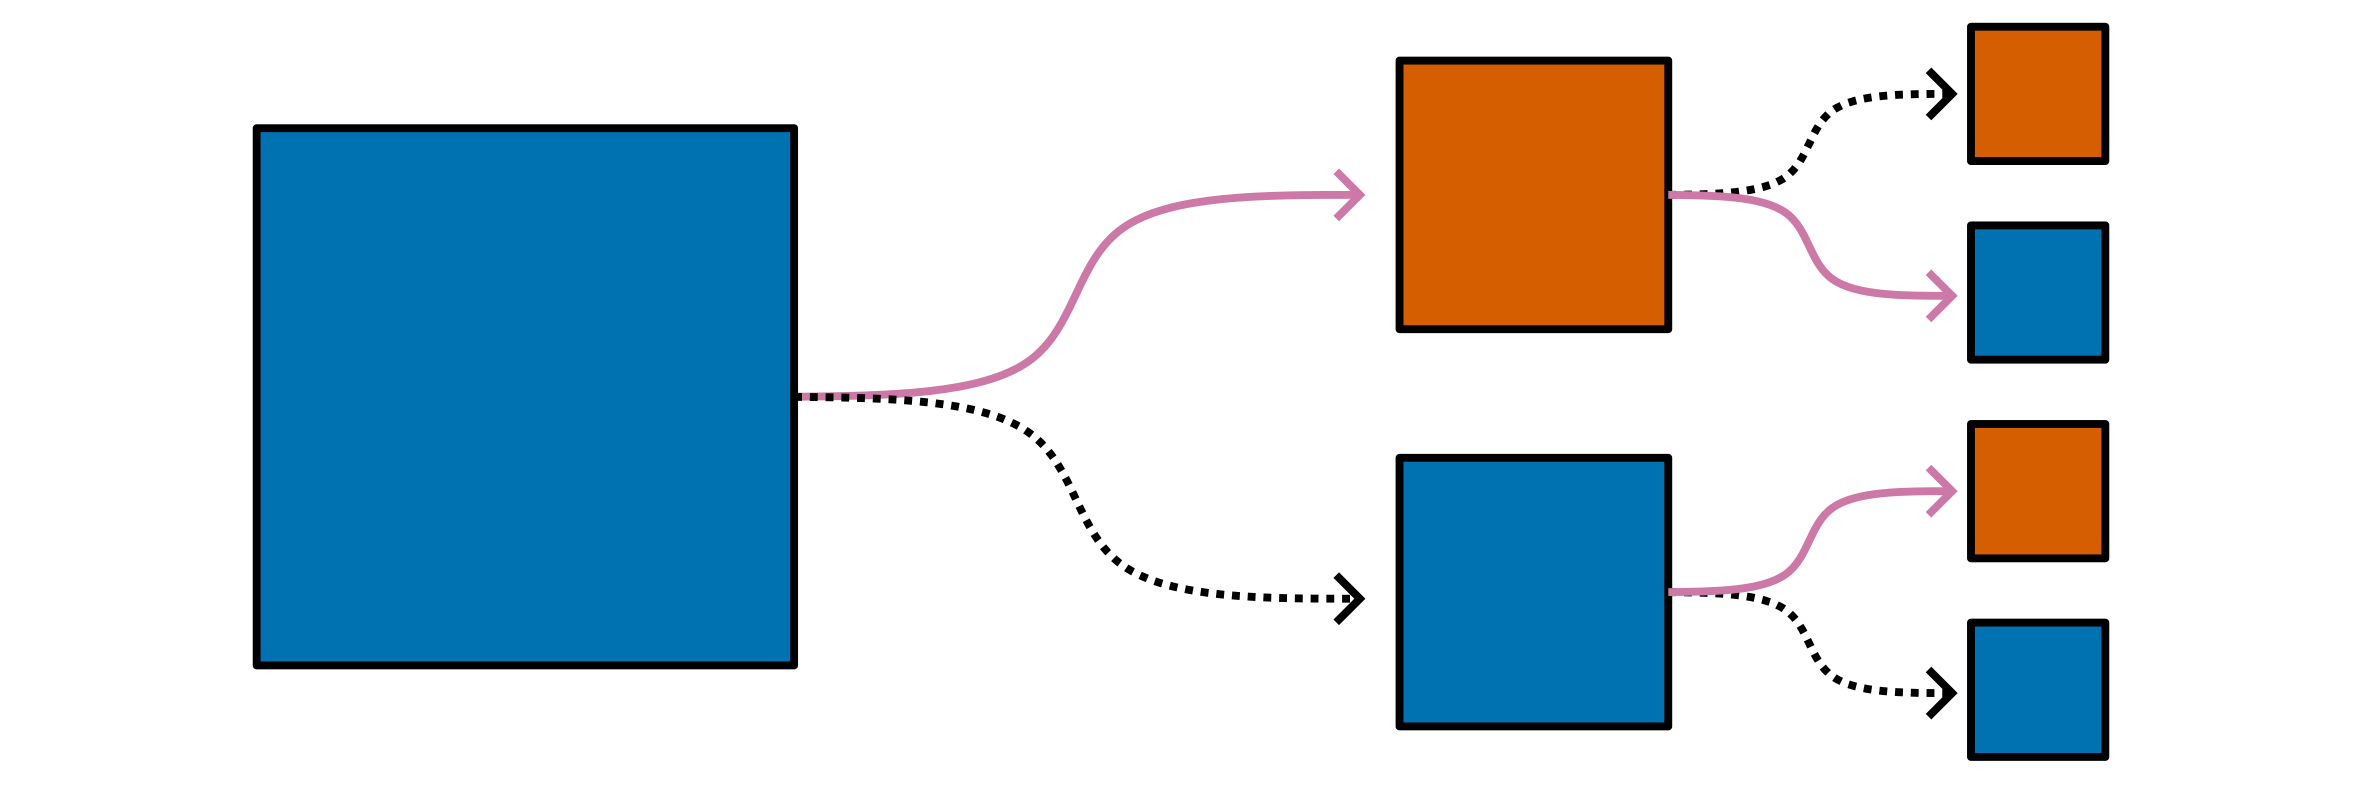
\includegraphics[width=\textwidth]{Figure 11.5.F}
\caption{A Markov chain for calculating cellular coldness}
\end{figure} \noindent
Coldness asks if a rotation increases or decreases the Shannon entropy of a cell. Whether the entropy increases or decreases depends on the transition from configuration $\hat X_i$ configuration $\hat X_j$. We might say that coldness $\beta$ of a cell is the dependent upon the conditional probability that a bit flip occurs.
$$\beta(x, t) = -\mathrm{E}[\log_2(p_{t+1}| p_t)] + \mathrm{E}[\log_2(p_{t})]$$
For a specific cell $x$ at time $t$ with rotation probability $p_t$, the thermodynamic beta depends upon the change in entropy \textit{presuming} that it rotates. 

If the cell performs a bit flip and the transition increases the Shannon entropy by a lot, the coldness is high. If the cell performs a bit flip and the transition increases the Shannon entropy by a little, the coldness is low. If the cell performs a bit flip and the transition decreases the Shannon entropy, the coldness is negative. If a cell does not rotate but the entropy increases or decreases, the coldness is either positive infinity or negative infinity respectively. This means that defining coldness for a single cell is inherently flawed.

\textbf{System coldness}\index{system coldness} $\beta$ is the discrete thermodynamic quantity for Boolean statistical mechanics that best matches the statistical mechanics definition and physics definition of thermodynamic beta. The systemic coldness $\beta$ is a matrix defined by the forward difference $\Delta_t$ of the entropy rate $R$ with respect to the forward difference of the internal energy $U$ such that:
$$\beta = \frac{\Delta_t R}{\Delta_t U}$$
We define the change in entropy rate as:
$$(\Delta_t R)_{(i, j)} | y_0 = -[(y_1) \log_2 (y_1)] - [y_{0} \log_2 (y_{0})]$$
We define teh change in internal energy as:
$$(\Delta_t U)_{(i, j)} | y_0 = \sum\limits_x \hat \eta_{i, j}(x)$$
Using the notation of a stochastic matrix $P$ and initial state vector $y_0$, we say that the change in entropy $\Delta R$ is given by the entropy of some definite future state $y_1$ minus the entropy of some definite initial state $y_0$. Likewise, the change in internal energy $\Delta U$ is the counts the number of cells that have rotated relative to a reference state.

As an aside, notice that if we used $\hat \sigma$ to count by full-rotations instead of $\hat \eta$ for half-rotations in our instead that we would need our formula to state:
$$(\Delta U)_{(i, j)} | y_0 = 2 \cdot \sum\limits_{x \in X} \hat \sigma_{(i, j)}(x)$$
Refer back to \textit{Figure 11.5} for an example planar state and \textit{Figure 11.8} for a frozen still state. The scaling by a factor of $2$ is used to distinguish the coldness of a planar state and a frozen still state for Boolean random walks. An initial state at $t=0$ may return to itself on $t = 2$ and all other even time states. Since the scaling is unnecessary in the half-rotation definition, the other definition is more ``natural''.

The lack of clarity in definition of energy is because there are multiple types of energy, but temperature specifically refers to internal energy $U$.\footnote{The common definition for the internal energy $U$ is the expected value of the system Hamiltonian. However, a specific transition from $\hat X_i$ to $\hat X_j$ has only one specific Hamiltonian for which a specific count of cells have rotated. This means our definition of $U$ identical to $E(H)$ in this context.} Notice that the coldness matrix $\beta$ depends on the transition from $\hat X_i$ to $\hat X_j$. To define the expectation of coldness $E(\beta)$, we likewise need to weight by probability of transition transition from $\hat X_i$ to $\hat X_j$. We cannot blindly define expectations as before because the $\beta$ matrix is defined by a first-order transition. This is not the \textit{expectation of a state}, but the \textit{expectation of a transition}.

Let us construct an example similar to \textit{Figure 11.9} to justify our definition. Suppose instead that we wish to apply this definition of coldness to a bounded simple random walk $\beta$. We might assign an energy level to each height and an entropy to the probability distribution. Suppose we start our random walk at the bottom of a tube:
\begin{figure}[H]
\centering
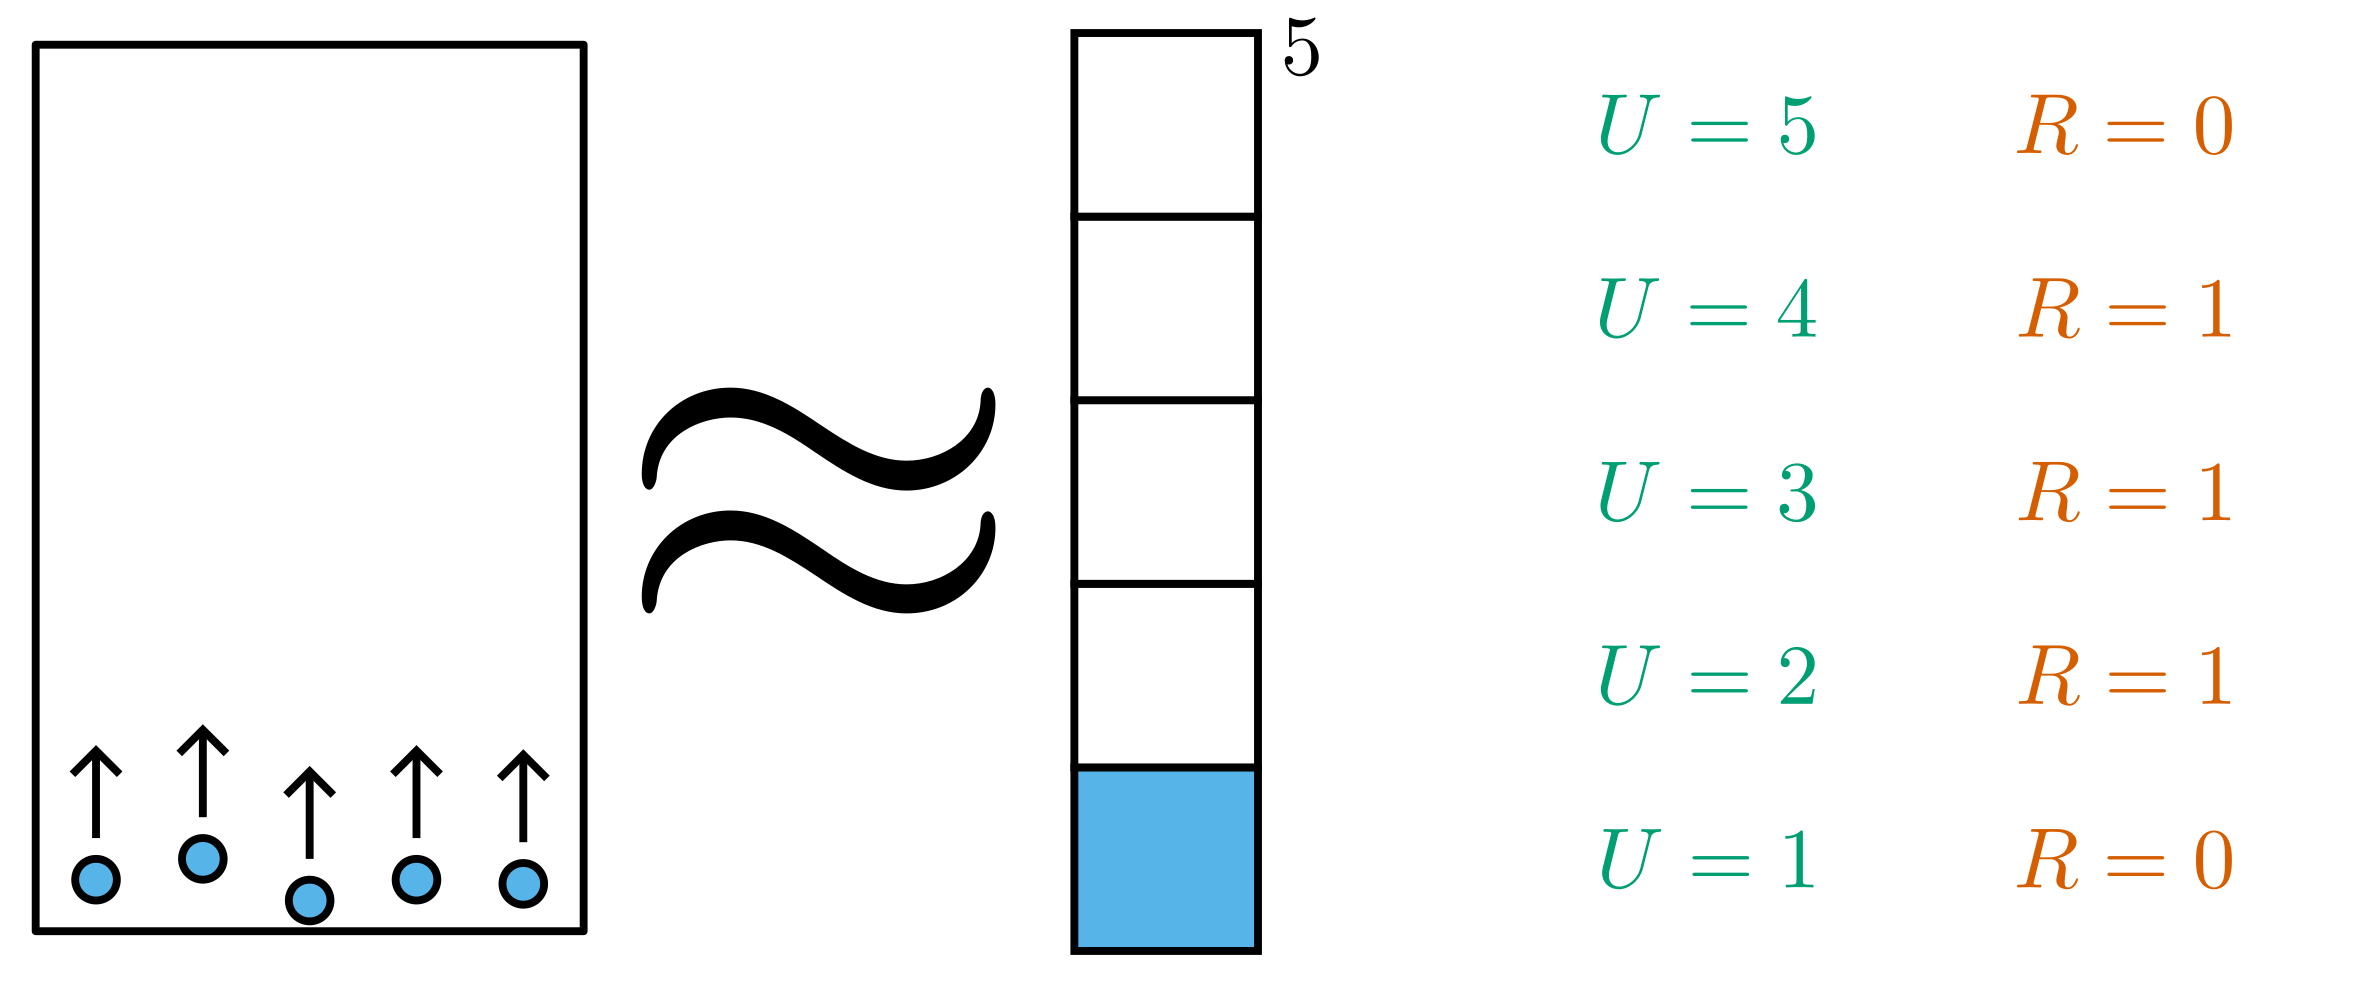
\includegraphics[width=\textwidth]{Figure 11.5.G}
\caption{The coldness $\beta$ of a transition matrix $P$ can be modeled using explicit demarcations of energy levels per state}
\end{figure} \noindent
Our random walks are independent, therefore we may calculate coldness by observing only one of the random walks. Since we start at the lowest energy level with only $1$ possible transition, the entropy is $R_0 = y_0 \cdot \log_2(y_0)$. The entropy after one time step is $R_1 = y_1 \cdot \log_2(y_1) = 1$ since it has an equal chance of moving up or down. The starting energy $U_0$ is the energy level $U = 1$ and the future energy $U_1$ is the energy level $U = 2$. Therefore the coldness is:
$$\beta = \frac{R_1 - R_0}{U_1 - U_0} = \frac{1-0}{1-0} = 1$$
If we start at the top energy level, we should obtain a coldness of $\beta = -1$.

We may calculate the coldness matrix $\beta$ for the previous example in the following way:
\[\renewcommand\arraystretch{2}\begin{bmatrix}
\frac{0-0}{1-1} & \frac{1-0}{2-1} & \frac{1-0}{3-1} & \frac{1-0}{4-1} & \frac{0-0}{5-1}\\
\frac{0-1}{1-2} & \frac{1-1}{2-2} & \frac{1-1}{3-2} & \frac{1-1}{4-2} & \frac{0-1}{5-2}\\
\frac{0-1}{1-3} & \frac{1-1}{2-3} & \frac{1-1}{3-3} & \frac{1-1}{4-3} & \frac{0-1}{5-3}\\
\frac{0-1}{1-4} & \frac{1-1}{2-4} & \frac{1-1}{3-4} & \frac{1-1}{4-4} & \frac{0-1}{5-4}\\
\frac{0-0}{1-5} & \frac{1-0}{2-5} & \frac{1-0}{3-5} & \frac{1-0}{4-5} & \frac{0-0}{5-5}\\
\end{bmatrix} 
=
\begin{bmatrix}
\frac{0}{0} & 1 & \frac{1}{2} & \frac{1}{3} & 0\\
1 & \frac{0}{0} & 0 & 0 & -\frac{1}{3}\\
\frac{1}{2} & 0 & \frac{0}{0} & 0 & -\frac{1}{2}\\
\frac{1}{3} & 0 & 0 & \frac{0}{0} & -1\\
0 & -\frac{1}{3} & -\frac{1}{2} & -1 & \frac{0}{0}\\
\end{bmatrix} 
\]
The convention for $0/0$ poses a problem for us. If we define $0/0=1$, the coldness matrix $\beta$ is symmetric matrix about the main diagonal and $\beta - I$ is skew-symmetric about the anti-diagonal. If we instead define the convention $0/0=0$, then coldness matrix $\beta$ is skew-symmetric about the anti-diagonal. 

The expected coldness vector $E(\beta)$ is $(1, 1/2, 0, -1/2, -1)$. The coldness matrix $\beta$ defines values for transitions that are impossible, and are therefore not used in the calculation. If we ``freeze'' a random walk state to transition into itself with some non-zero probability, then the convention that $0/0 = 1$ is the most intuitive and consistent. This ``freezing'' would increase the coldness of each state, as a ``colder particle'' is slower the deviate from its original position.

Let us define the \textbf{entropy rate}\index{entropy rate} $R_i$ of a stochastic matrix $P$ starting from state $\hat X_i$ as:
$$R_i = -\sum\limits_{j=1}^\theta P_{(i, j)} \log_2(P_{(i, j)})$$
We use $\log_2$ is in terms of bits or shannons for convenience of Boolean statistical mechanics. We define a matrix $\Delta R$ as having the elements:
$$(\Delta R)_{(i, j)} = R_j - R_i$$
This the change in entropy rate as a state moves from state $\hat X_i$ to state $\hat X_j$. The definition for entropy rate should give us an intuitive interpretation of Boolean random walks. A planar state will have a positive coldness because its entropy increases as cells rotate, and each of the two halves is a frozen state. A checkerboard state will have negative coldness because its entropy will decrease as cells rotate.

Let us define some measure of the change in the internal energy $\Delta U$ as the change in the angular momentum per unit of time as:
$$(\Delta U)_{(i, j)} = \sum\limits_{x \in X} \eta_{(i, j)}(x)$$
It adds up all of the changes in angular momentum from state $\hat X_i$ to state $\hat X_j$. Change in the internal energy $\Delta U$ is appropriate because the physics definition of change in internal energy refers to $E_i$ as the energy required to transition from some reference state to some other state for each $i$:
$$\Delta U = \sum E_i$$
Our Boolean statistical mechanics definition refers to the sum of energy transfers needed to change from state $\hat X_i$ to state $\hat X_j$. 

In terms of Boolean random walks, the summation counts the number of bit flip pairs since each bit's flip is worth $\frac{1}{2}$ units of energy.\footnote{If we are using $x \in \{-i, +i\}$ for all $x \in X$, then $\eta$ should be given by $\eta = \ln(\mathcal X^* \otimes X)/(\pi i)$ in which $\mathcal X^*$ provides the complex conjugate of states in $\mathcal X$. Remember that $1/i = -i$.} As discussed in \textit{\S 9.5 Issues in Defining Energy}, a Boolean signal of $f \in \{-1, +1\}$ has constant energy but measurable \textit{changes} in the signal $f$.

We may define the system coldness matrix $\beta$ as:
$$\beta = \frac{\Delta R}{\Delta U}$$
Thus, the expected coldness vector $E(\beta)$ of a system at time $t$ is:
$$\langle \beta \rangle_t | y_0 = (y_0 (P^t \odot \beta)) \cdot \textbf{1}$$
for a given stochastic matrix $P$ and initial distribution $y_0$. We may define the expected coldness of any given initial state by replacing $y_0$ with the identity matrix:
$$\langle \beta \rangle_t = (I (P^t \odot \beta)) \cdot \textbf{1}$$
This definition is what gives us the calculation for the expected coldness vector for the system in \textit{Figure 11.11}. 

The \textbf{distribution coldness}\index{distribution coldness} $\alpha$ is a vector is defined as:
$$\alpha_t = \frac{\Delta S}{\Delta H} = \frac{
-\sum\limits_j [P^{t+1}_{(i, j)} \log_2(P^{t+1}_{(i, j)})]
+ \sum\limits_j[P^t_{(i, j)} \log_2(P^t_{(i, j)})]
}{
[\sum\limits_j P^{t+1}_{(i, j)} - P^t_{(i, j)}](P \odot \hat \eta)
} $$
We calculate $\alpha$ for an initial condition by choosing the appropriate row corresponding to it. 

This alternative definition of coldness is very different because it is the ratio of entropy rate and the bit rate at a distribution level:
\begin{figure}[H]
\centering
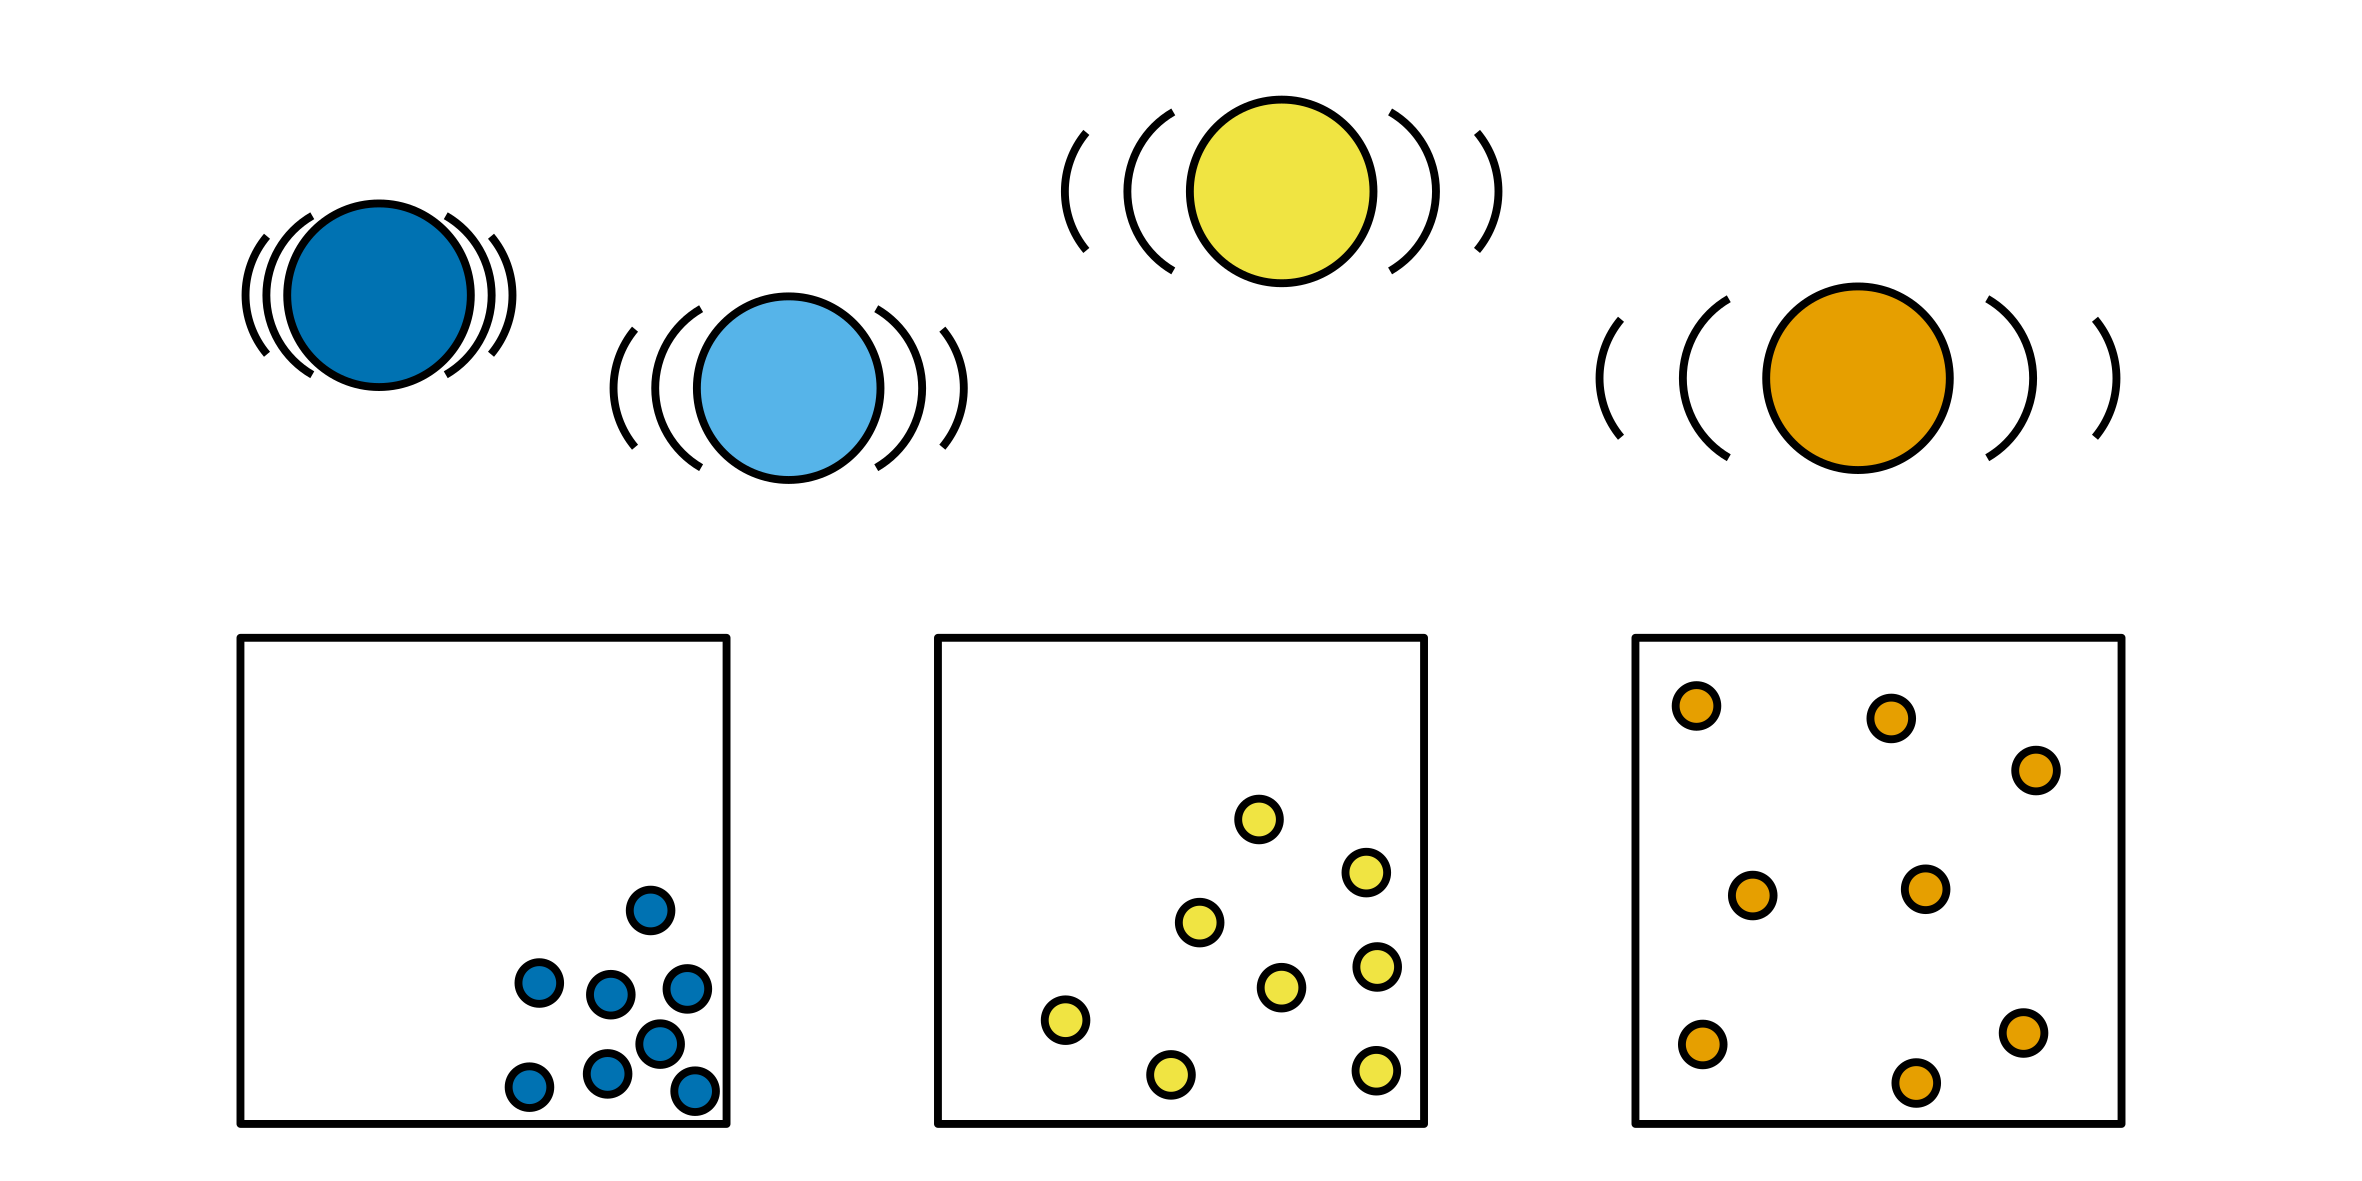
\includegraphics[width=\textwidth]{Figure 11.5.H}
\caption{The distribution coldness of warm particles decreases faster because the entropy rate is faster}
\end{figure} \noindent
\noindent % N boxes containing 1 particle each.
Similar to the earlier example in which we ``freeze'' a random walk, the system coldness of the colder particles is higher than the warmer particles. The distribution coldness of the cold particles is always higher than the distribution coldness of the warm particles because of the diffusion resistance from standing still.

Once at equilibrium, any action that they take does not result in a positive change in entropy. Since the change in entropy is dictated by the eigenvalues of transition matrix $P$, distribution the coldness always converges to $0$. Once a specific state is determined, the distribution coldness and temperature ``reset''. The distribution coldness is always decreasing if the system is aperiodic, and it is always decreasing with respect to the period of the system. An example where periodicity matters is a $2$-periodic system with $6$ ``odd states'' and $2$ ``even'' states, resulting in a fluctuating temperature due to the size imbalance but still is monotonically decreasing with respect to period $2$.

This is unlike system coldness whose expectation is a convex sum of coldness entries. For the freezing of the random walk pictured in \textit{Figure 11.11}, the average system coldness of a probability vector $y_s$ is exactly the dot product between $y_s$ and $\textnormal{diag}(P)$. In other words, system coldness has no obligation to converge to $0$.

We now have a proper constructive definition of coldness as derived from the analysis of discrete thermodynamics.\footnote{Inaccurate conclusions about the second law of thermodynamics are derived from confusion between system coldness and distribution coldness.} As for most things in Boolean statistical mechanics, the system coldness matrix $\beta$ is likely not practically computable. Instead of measuring the coldness of a whole system, we can measure the coldness of smaller systems such as a $3 \times 3$ subsystem in a $100 \times 100$ system. From there, we can assign a temperature to each cell based upon its $3 \times 3$ block. We can also define coldness to exist for any Boolean mechanical system that is not Boolean random walks in particular.

\section{Boolean Crystallography}
\textbf{Crystallography}\index{crystallography} is concerned with the mathematical methods that may analyze the molecular and crystalline structure of solids. Crystallinity is informally classified into four categories on a scale of regular crystallinity and amorphous glass:
\begin{enumerate}
\item Holocrystalline: Fully crystalline
\item Hypocrystalline: Partially crystalline
\item Hypohyaline: Partially glass
\item Holohyaline: Fully glass
\end{enumerate}
Crystals are low entropy structures while glasses are high entropy structures. We are not interested in crystallography for how it analyzes lattices in continuous space; we are interested in how its methods may help us understand lattice thermodynamics.

The \textbf{reciprocal lattice}\index{reciprocal lattice} is the Fourier transform of a direct lattice. If the direct lattice is the position space, then the reciprocal lattice is the momentum space. For example, the spatial distribution of electron density for a crystal's molecular structure:
\begin{figure}[H]
\centering

\includegraphics[width=\textwidth]{Figure 11.6.A}
\caption{The direct lattice of an example electromagnetic field}
\end{figure} \noindent
\noindent % The direct lattice of the position electron density distribution
has a frequency distribution that denotes the magnitude of each frequency that composes the electron density position distribution:
\begin{figure}[H]
\centering
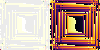
\includegraphics[width=\textwidth]{Figure 11.6.B}
\caption{The reciprocal lattice of the prior electromagnetic field}
\end{figure} \noindent
\noindent % The reciprocal lattice of the momentum electron density distribution
This reciprocal lattice was created via the Fourier transform of the position lattice. For the left image, transparency indicates magnitude while color indicates phase. For the right image, transparency is removed to make visualizing phase easier. In a rectangular lattice, the peaks of the Fourier transform are at integer multiples of $2 \pi / \ell$.

In Boolean statistical mechanics, the eigendecomposition $P = \Phi \Lambda \Phi^{-1}$ has column eigenvectors that are denoted by $| \phi \rangle$. The eigenvalues $\lambda_1,...,\lambda_\theta$ that are each associated with eigenvectors $| \phi_1 \rangle ,..., |\phi_\theta \rangle$ correspond to a momentum field given by the harmonic eigenstates $\hat A_1,..., \hat A_\theta$:
$$\hat A_j = \sum\limits_{i=1}^\theta \Phi_{(i, j)} \hat X_i$$
Each configuration eigenstate $\hat X_i$ has a Boolean value upon each position coordinate $x = (x_1,...,x_d)$, therefore the linear mapping of configuration eigenstates to the harmonic eigenstates means that each harmonic eigenstate has an associated complex value upon each position $x$. 

Instead of performing a Fourier transform of a configuration eigenstate $\hat X_i$, we can obtain its finite countable momentum composition if and only if the harmonic eigenstates $\hat A = \hat A_1 ,..., \hat A_\theta$ are exactly the wavevectors on the direct lattice $X$. If they are, then we may use a finitely countable Fourier transform. If not, then the harmonic eigenstates represent a more general harmonic on the lattice. In either case, the eigenvalues $\lambda_1 ,...,\lambda_\theta$ corresponding to eigenvectors $| \phi_1 \rangle ,..., |\phi_\theta \rangle$ must lie within the unit complex disc:
\begin{figure}[H]
\centering
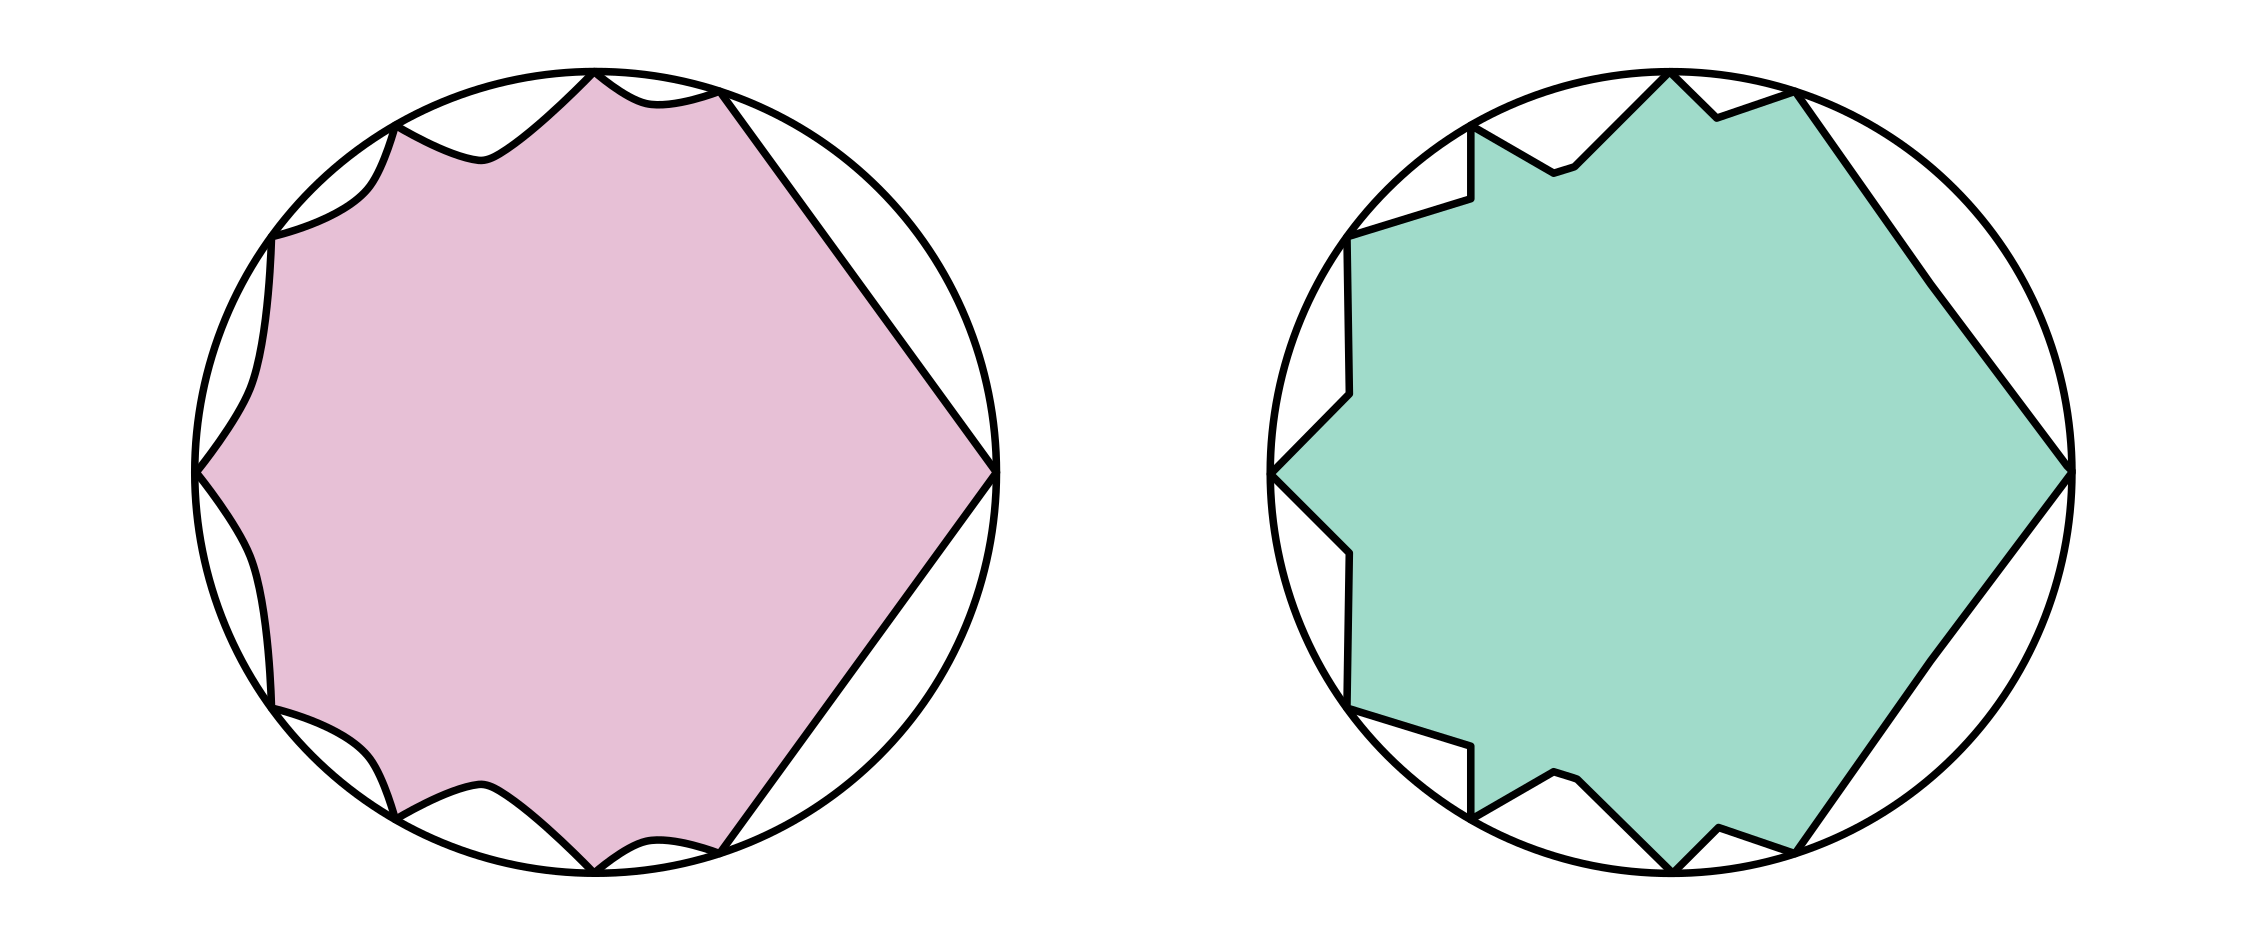
\includegraphics[width=\textwidth]{Figure 11.6.C}
\caption{The Karpelevich region of a $5 \times 5$ transition matrix in purple, its polygon approximation in green}
\end{figure} \noindent
\noindent % The unit complex disc
in a way that produces the transition probabilities on the stochastic transition matrix $P$. For Boolean random walks, these transition probabilities are rational.

Crystallinity versus hyalinity corresponds to some measure of purity with respect to some eigenbasis:
\begin{figure}[H]
\centering
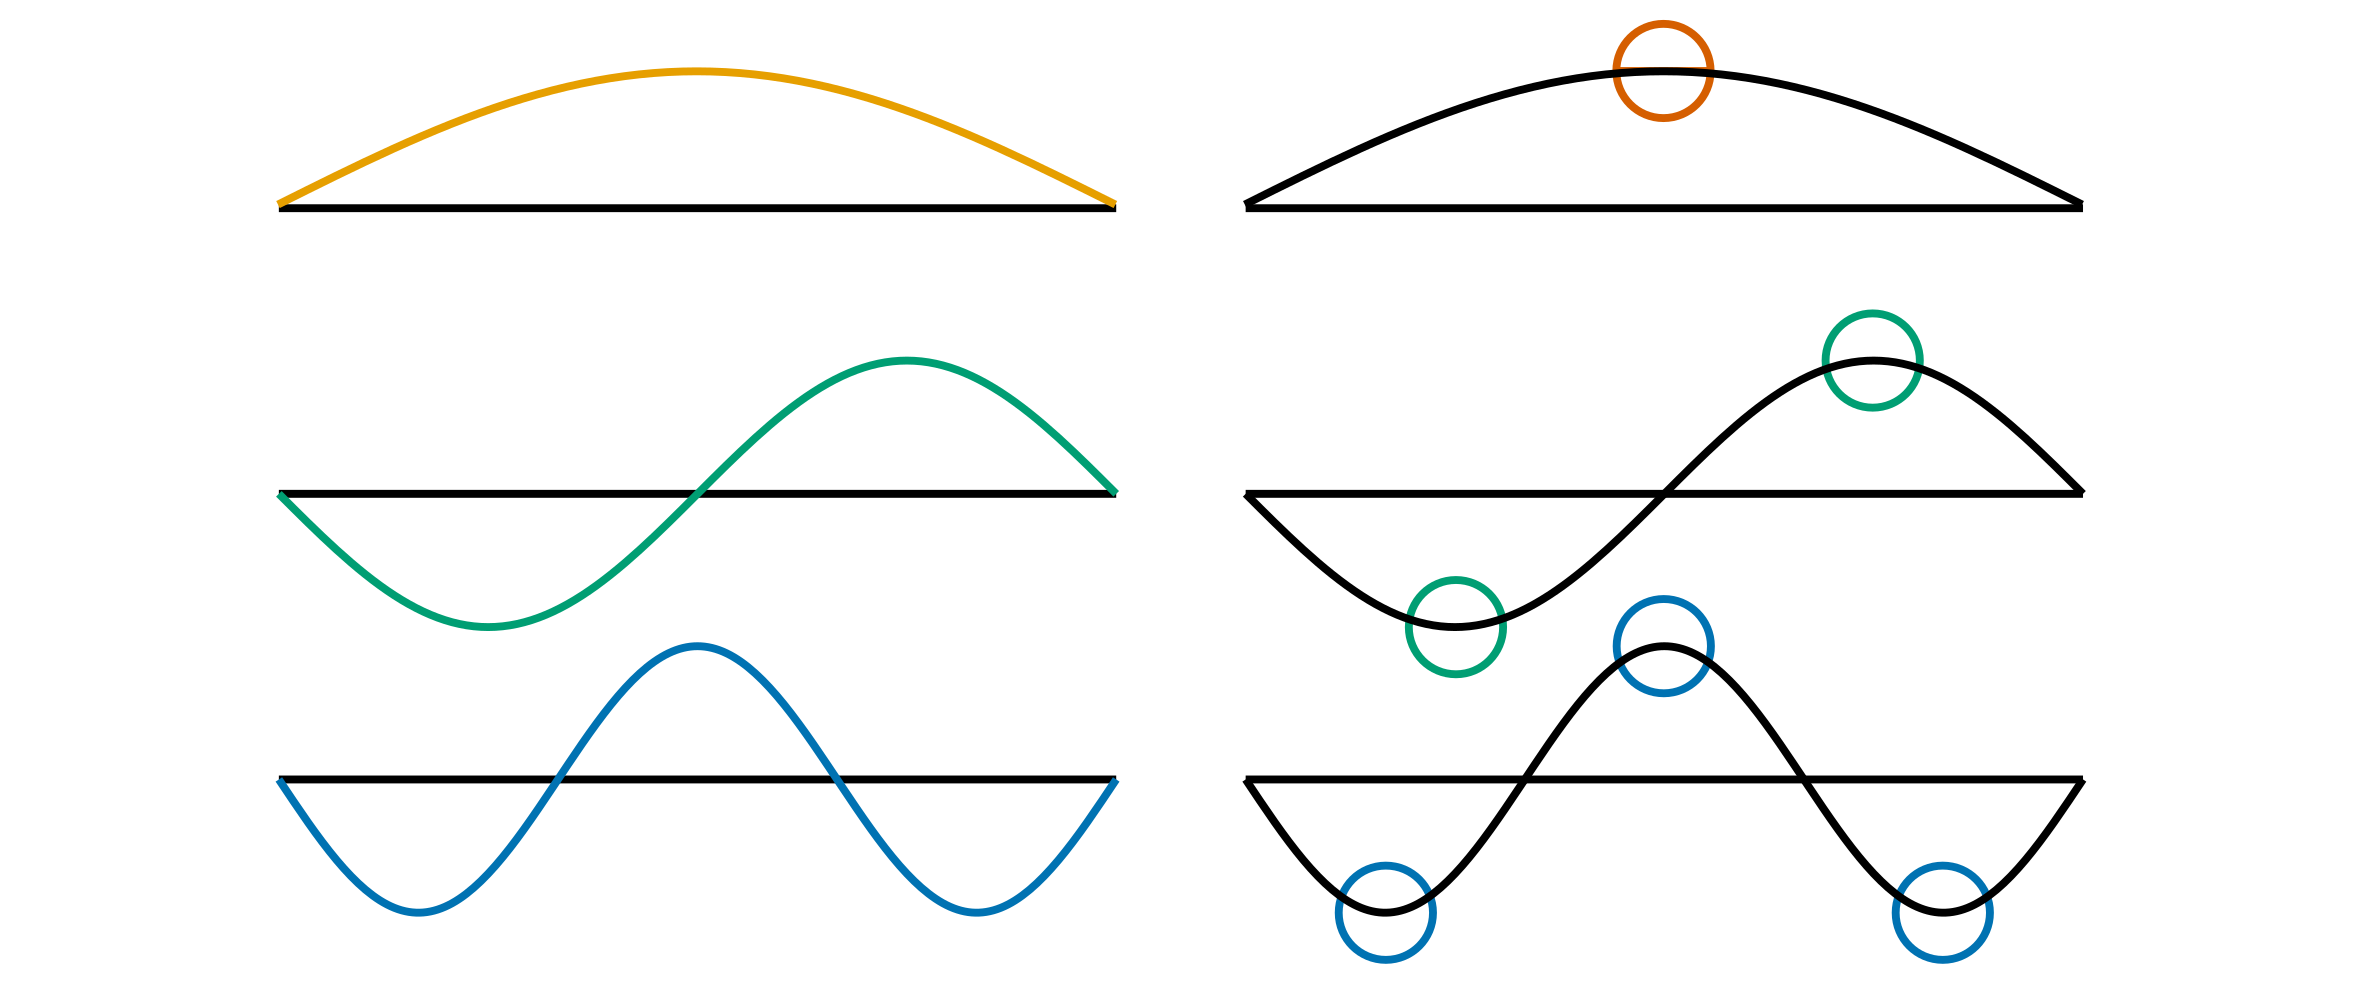
\includegraphics[width=\textwidth]{Figure 11.6.D}
\caption{A crystal should be periodic with respect to its ``high points''}
\end{figure}
\noindent % The first, second, and third normal modes of a string
The harmonics of a stringed instrument are periodic, meaning that the structure repeats its highs and lows. Crystalline materials like diamonds are highly periodic. Hyaline materials like obsidian are highly aperiodic. 

What would be a proper measure of the purity of a momentum composition? I have no answer. A Boolean direct lattice has a reciprocal lattice that itself appears periodic:
\begin{figure}[H]
\centering
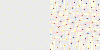
\includegraphics[width=\textwidth]{Figure 11.6.E}
\caption{The deconvolution of the example electromagnetic field direct lattice and the corresponding reciprocal lattice}
\end{figure}
\noindent
Without the blurring of a density field, it is possible to see that a crystalline structure in the reciprocal lattice.

An important question to ask is this: is a macroparticle necessarily crystalline? A macroparticle is in some sense a temporally regular structure. It may not necessarily occur in the same space nor in the same configuration since it may draw from a set of possible states, but together the states are meta-stable or semi-stable. As discussed in \textit{\S 11.3 Boolean Hamiltonians}, the system should tend towards potential wells in order to minimize its free energy. Is the potential well for a meta-stable macroparticle a crystal in the state space? How does this relate to temperature?

The Greek word $\kappa \rho \acute \upsilon \sigma \tau \alpha \lambda \lambda o \varsigma$ (kr\'{u}stallos) means clear ice or rock crystal. For a given material, the solid state has a lower temperature than its liquid state. We may alternatively state that a solid state has a greater coldness $\beta$ than a liquid state. Is system coldness $\beta$ a better representation of the regularity of a structure? Does coldness necessarily represent a crystalline structure for a Boolean random walk? Does coldness imply a crystalline structure for a Boolean statistical mechanics in general?

\section{Macroparticle Creation and Annihilation}
\textbf{Solitons}\index{soliton} are strongly stable wave packets, and they may be considered to be self-stabilizing or self-computing. Solitons occur in a variety of media such as electromagnetic fields or water, even resisting a river's current:
\begin{figure}[H]
\centering
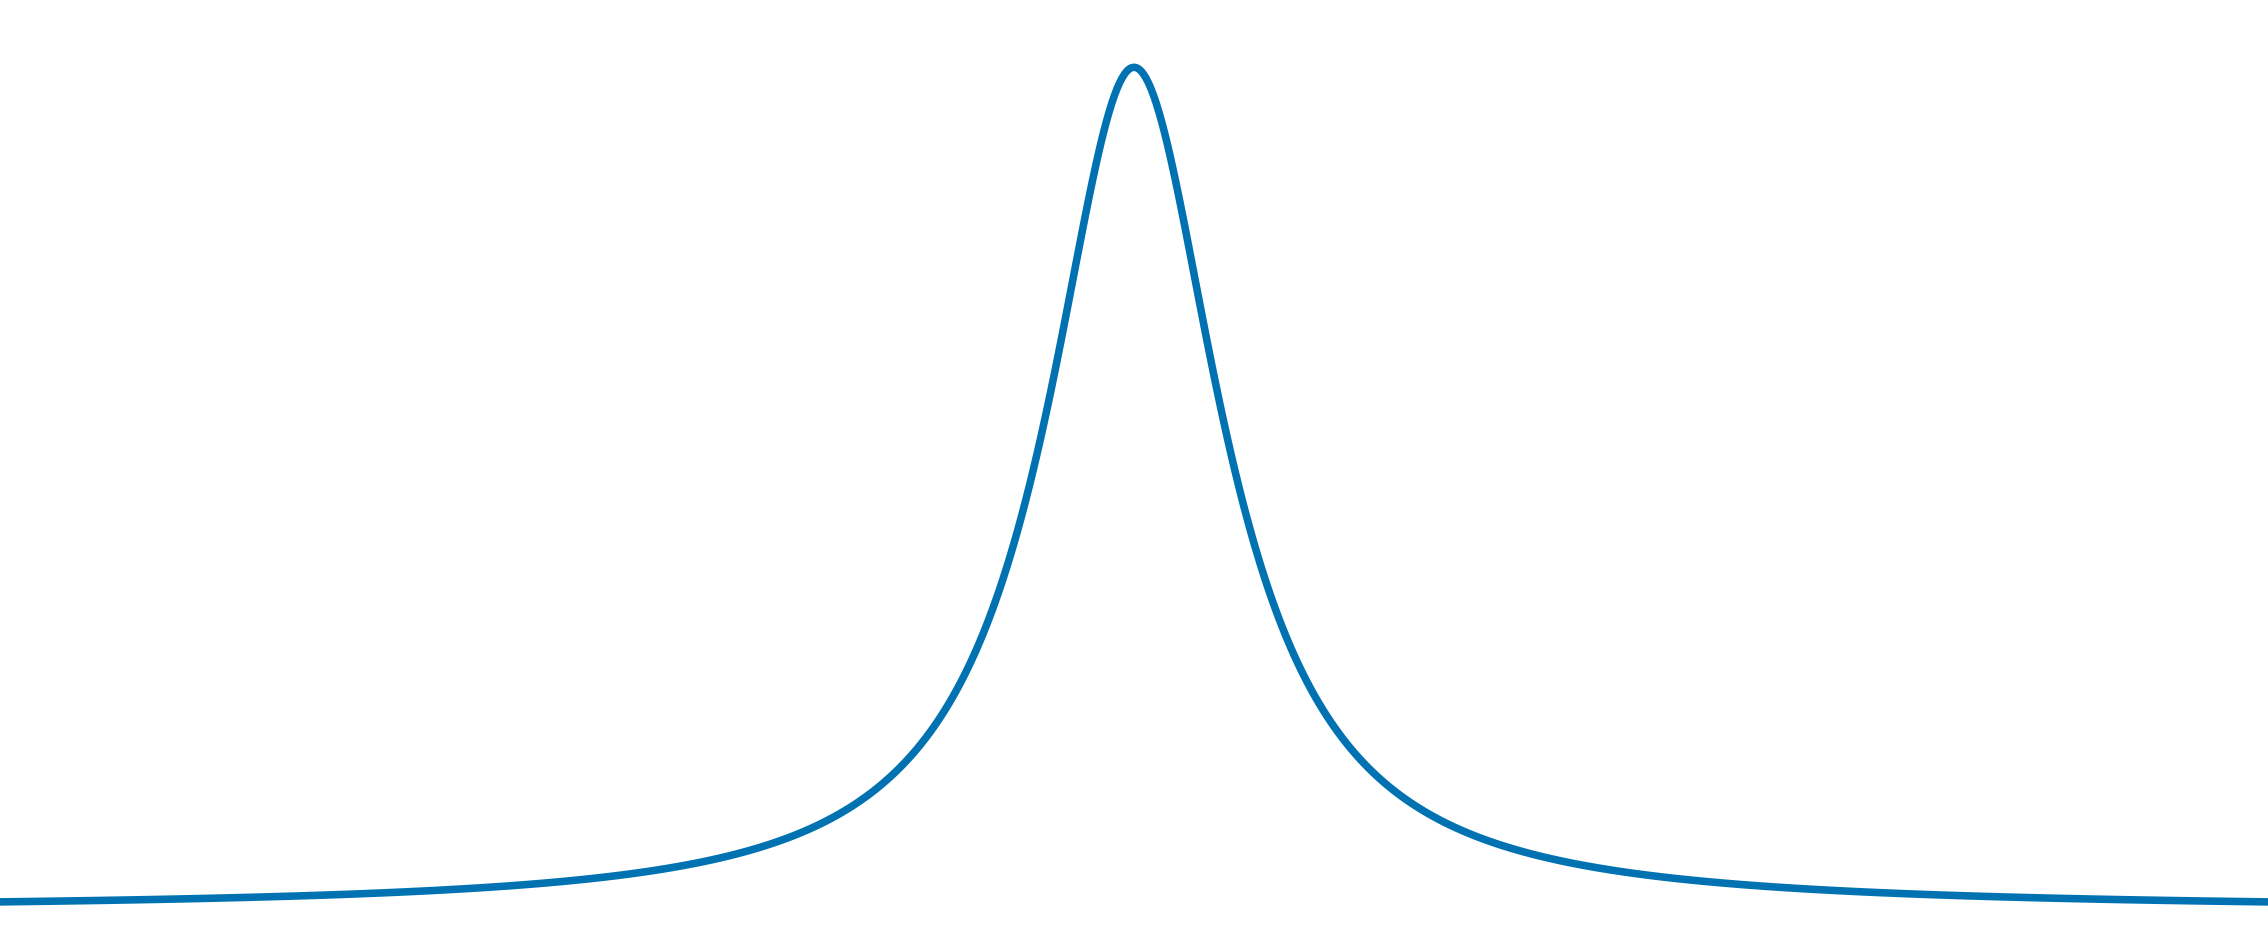
\includegraphics[width=\textwidth]{Figure 11.7.A}
\caption{A Peregrine soliton as a solution to the Schr\"{o}dinger equation}
\end{figure} \noindent
\noindent % An image of a soliton, a solitary wave
A soliton resists disruption via collision with other wave packets or self-destruction into the medium's vacuum state. Solutions to the Schr\"{o}dinger equation describe solitons that occur in media governed by the equation. If the soliton oscillates, then it is known as a breather.

Solitons and breathers are of the utmost important to particle theorists because they contradict the expectations of diffusion-type equations. Instead of diffusing, these structures are self-reinforcing. On a lattice, discrete solitons and discrete breathers are directly influenced by the connection strengths and specific shape of the lattice.

Boolean statistical mechanics via Boolean random walks gives rise to weakly stable wave packets even for small simulations. They are visible by smoothing the simulation with a smoothing filter like Gaussian or Multinomial, and the filter's radius or variance affects the produced image:
\begin{figure}[H]
\centering
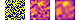
\includegraphics[width=\textwidth]{Figure 11.7.B}
\caption{A Boolean random walk and a smoothing filter. Smoother filters wash out smaller patterns but make larger structures more obvious.}
\end{figure} \noindent
\noindent % A raw Boolean state, a Multinomial(10) smoothed version of the raw state, and a Multinomial(20) smoothed version of the raw state
Larger solitons would require larger simulations using my faster algorithm developed in 2024 as discussed in \textit{\S Appendix E: Random Backtrack Algorithm}. It also requires some kind of spatio-temporal smoothing, so defining what is or is not a particle has some level of subjectivity if determined by this manner.

The main flaw of quantum mechanics is that its simulations require specifying particles as elements separate from their quantum field. Despite the fact particles are unique patterns as mere subsets of the field, their spontaneous generation or self-stabilizing mechanism cannot currently be formally described. A hydrogen atom's electron may be described as ``folding'' its probability density function when it absorbs and release a photon. 

The spontaneous creation and annihilation of electron-position pairs may not be described this way. An electron must be strongly stable in the presence of vacuum fluctuations while potentially emerging from vacuum fluctuations:
\begin{figure}[H]
\centering
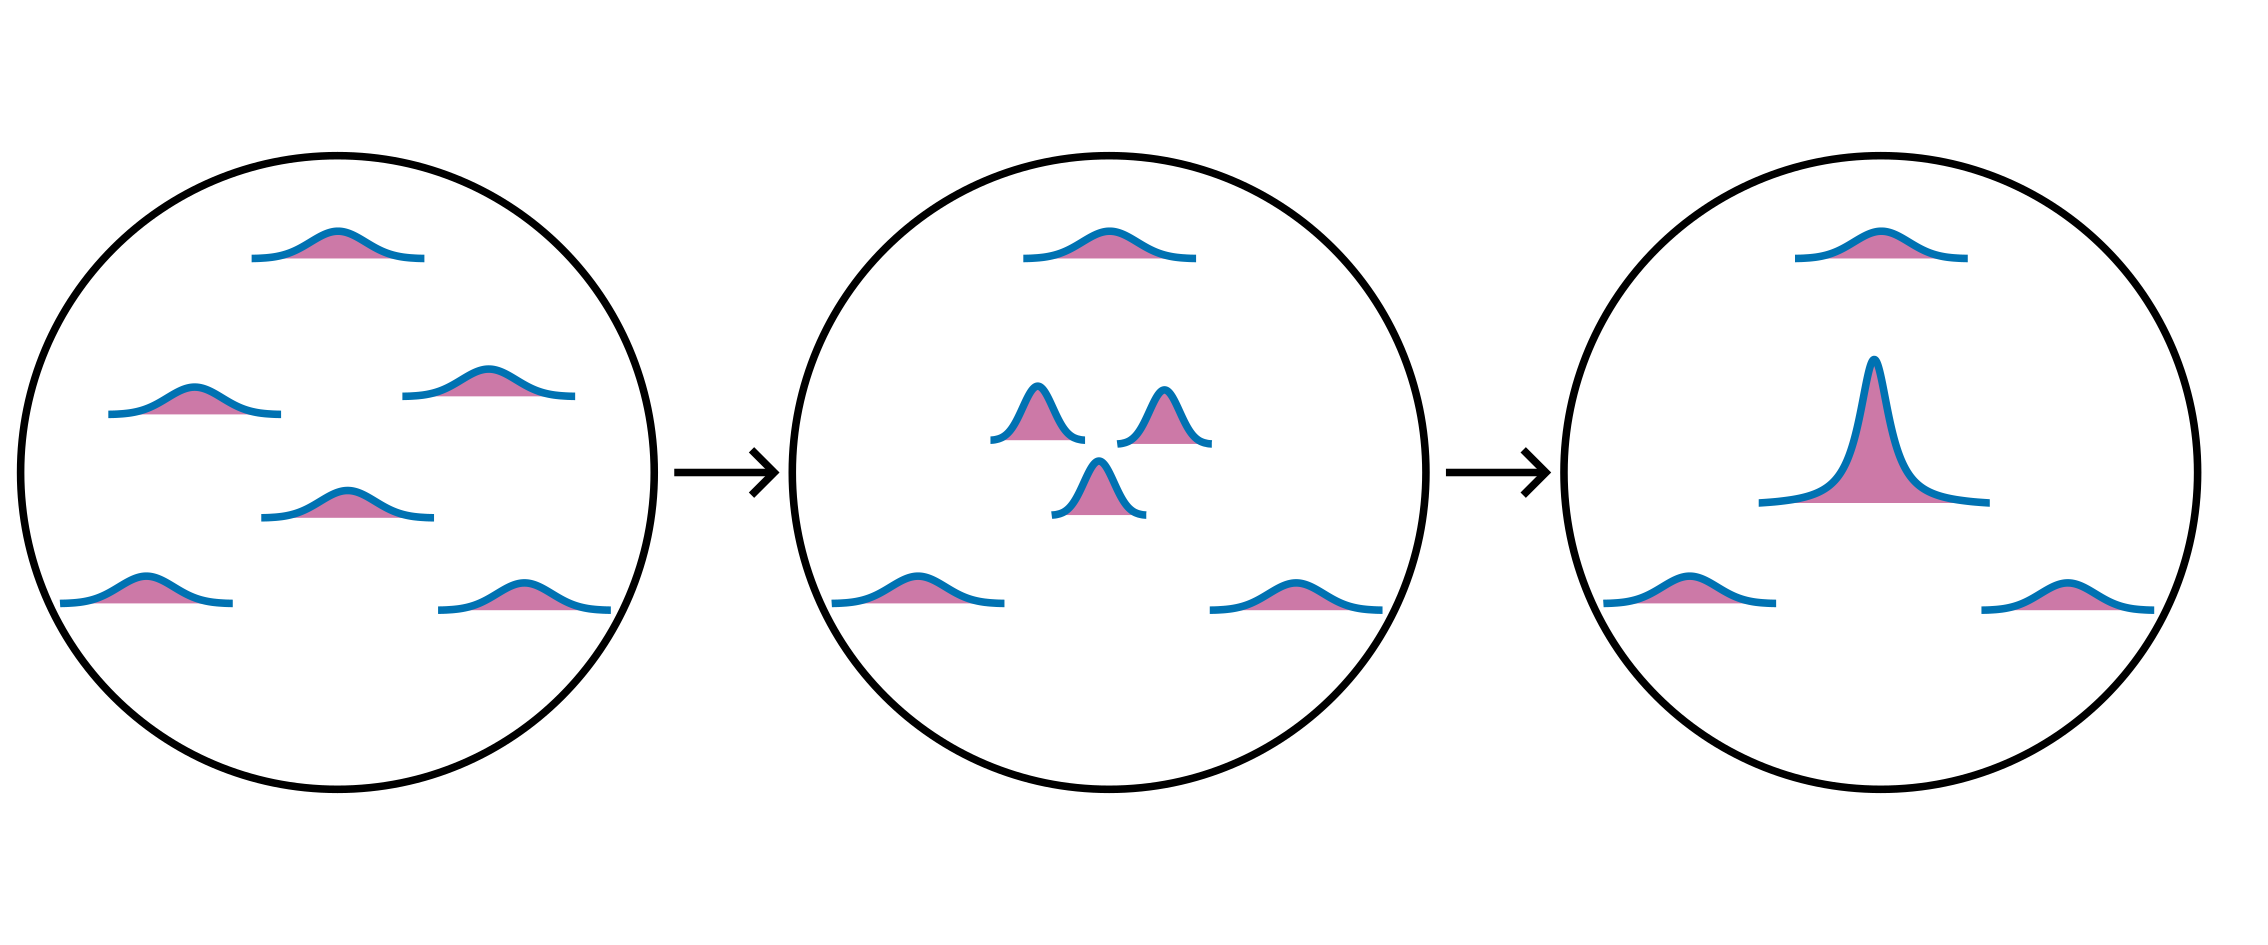
\includegraphics[width=\textwidth]{Figure 11.7.C}
\caption{A representation of a fluctuation that may spontaneously create a particle}
\end{figure} \noindent
\noindent % A sequence of vacuum fluctuations that results in the creation of an electron
There must be some sequence of states in the vacuum that increases or decreases the probability that there will be an electron at some point in the future, and there must be a way to count them.

In Boolean statistical mechanics, we seek to find special sets of states with highly collinear futures called eigenclasses. For example, let $g \in G$ be a specific state in the class $G$ in which all states have the same structure and volume:
\begin{figure}[H]
\centering
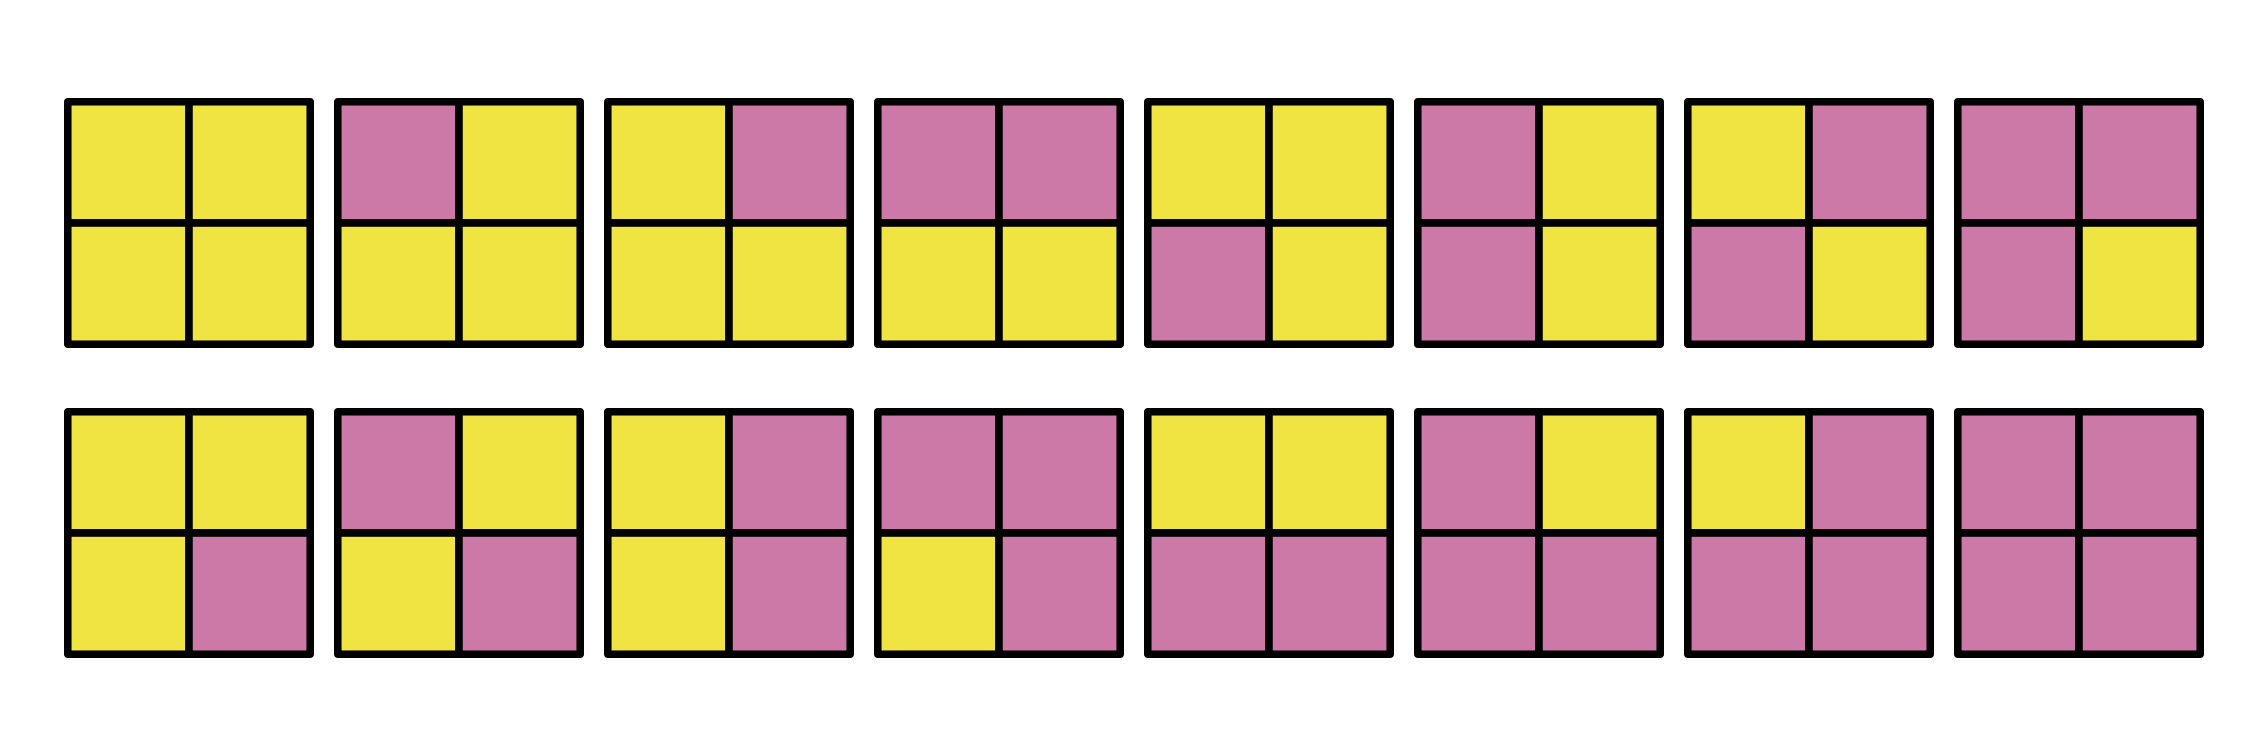
\includegraphics[width=\textwidth]{Figure 11.7.D}
\caption{States $g_1,...,g_{16}$ compose the class $G$. Notice that this list is symmetric with respect to reversal and Boolean inversion, implying that the transition matrix $P$ the $k$-the row the reverse of the $(\theta-k)$-the row}
\end{figure} \noindent
\noindent % A specific 2x2 state makes up g_1, but all 2x2s make up G
For example, a specific $2 \times 2$ may is indicated by $g_1$, and each $g_i$ is an element of $G$. We normally do not make a class the whole state space $\mathcal X$ but a subset. To find a subset $G$, we need to categorize rows of $P^{t}$ based upon how similar they are after some finite time for $t$.

We state that $\tilde g_i$ is some normalization upon $g_i$. Since each Boolean cell is from the set $\mathbb B_\pm = \{-1, +1\}$, we divide by the number of cells $n$ so that the measure of each cell is from the set $\{-1/n, +1/n\}$. By convolving $\tilde g_i(x)$ with the whole system $f(x,t)$, we obtain a measure of the ``purity'' of pattern $g_i$ for each position and time coordinate $(x, t)$. We call the class $G$ \textit{bosonic} if every state and its anti-state are in $G$:
$$-g_i \in G, \ \forall g_i \in G$$
We call the class $G$ \textit{fermionic} if some or none of its anti-states are in $G$:
$$-g_i \notin G, \ \exists g_i \in G$$
Bosonic classes contain their anti-states while fermionic classes may contain some, preferably none.

By convolving a normalized state $\tilde g_i(x)$ with the Boolean mechanical system $f(x, t)$, we obtain a rational number from the set $[-1, +1]$ for fermionic classes or a rational number between $[0, 1]$ for bosonic classes. We call $\omega_i(x, t) = f(x, t) * \tilde g_i(x)$ the \textit{raw frequency} of $\tilde g_i(x)$ at $f(x, t)$, or the convolution of $f$ and $\tilde g_i$. Convolution with a normalized function measures the similarity of two functions at each point in space and time $(x, t)$. We must choose a convention for handling multiple choices of $\omega_i$ per cell because there may be many rotated variations of an identified macroparticle in $3$-dimensions.

Before deciding a count convention, we must acknowledge that the measure $\omega_i(x, t)$ permits or implies the existence of virtual particles. For $(1 - \varepsilon) < |\omega_i| 1$ in which the error is very small $\varepsilon > 0$, the region with an erroneous particle is computationally indistinguishable from $g_i$ for interactions over very small time scales. However, this virtual particle may not be stable because it contains interior defects:
\begin{figure}[H]
\centering
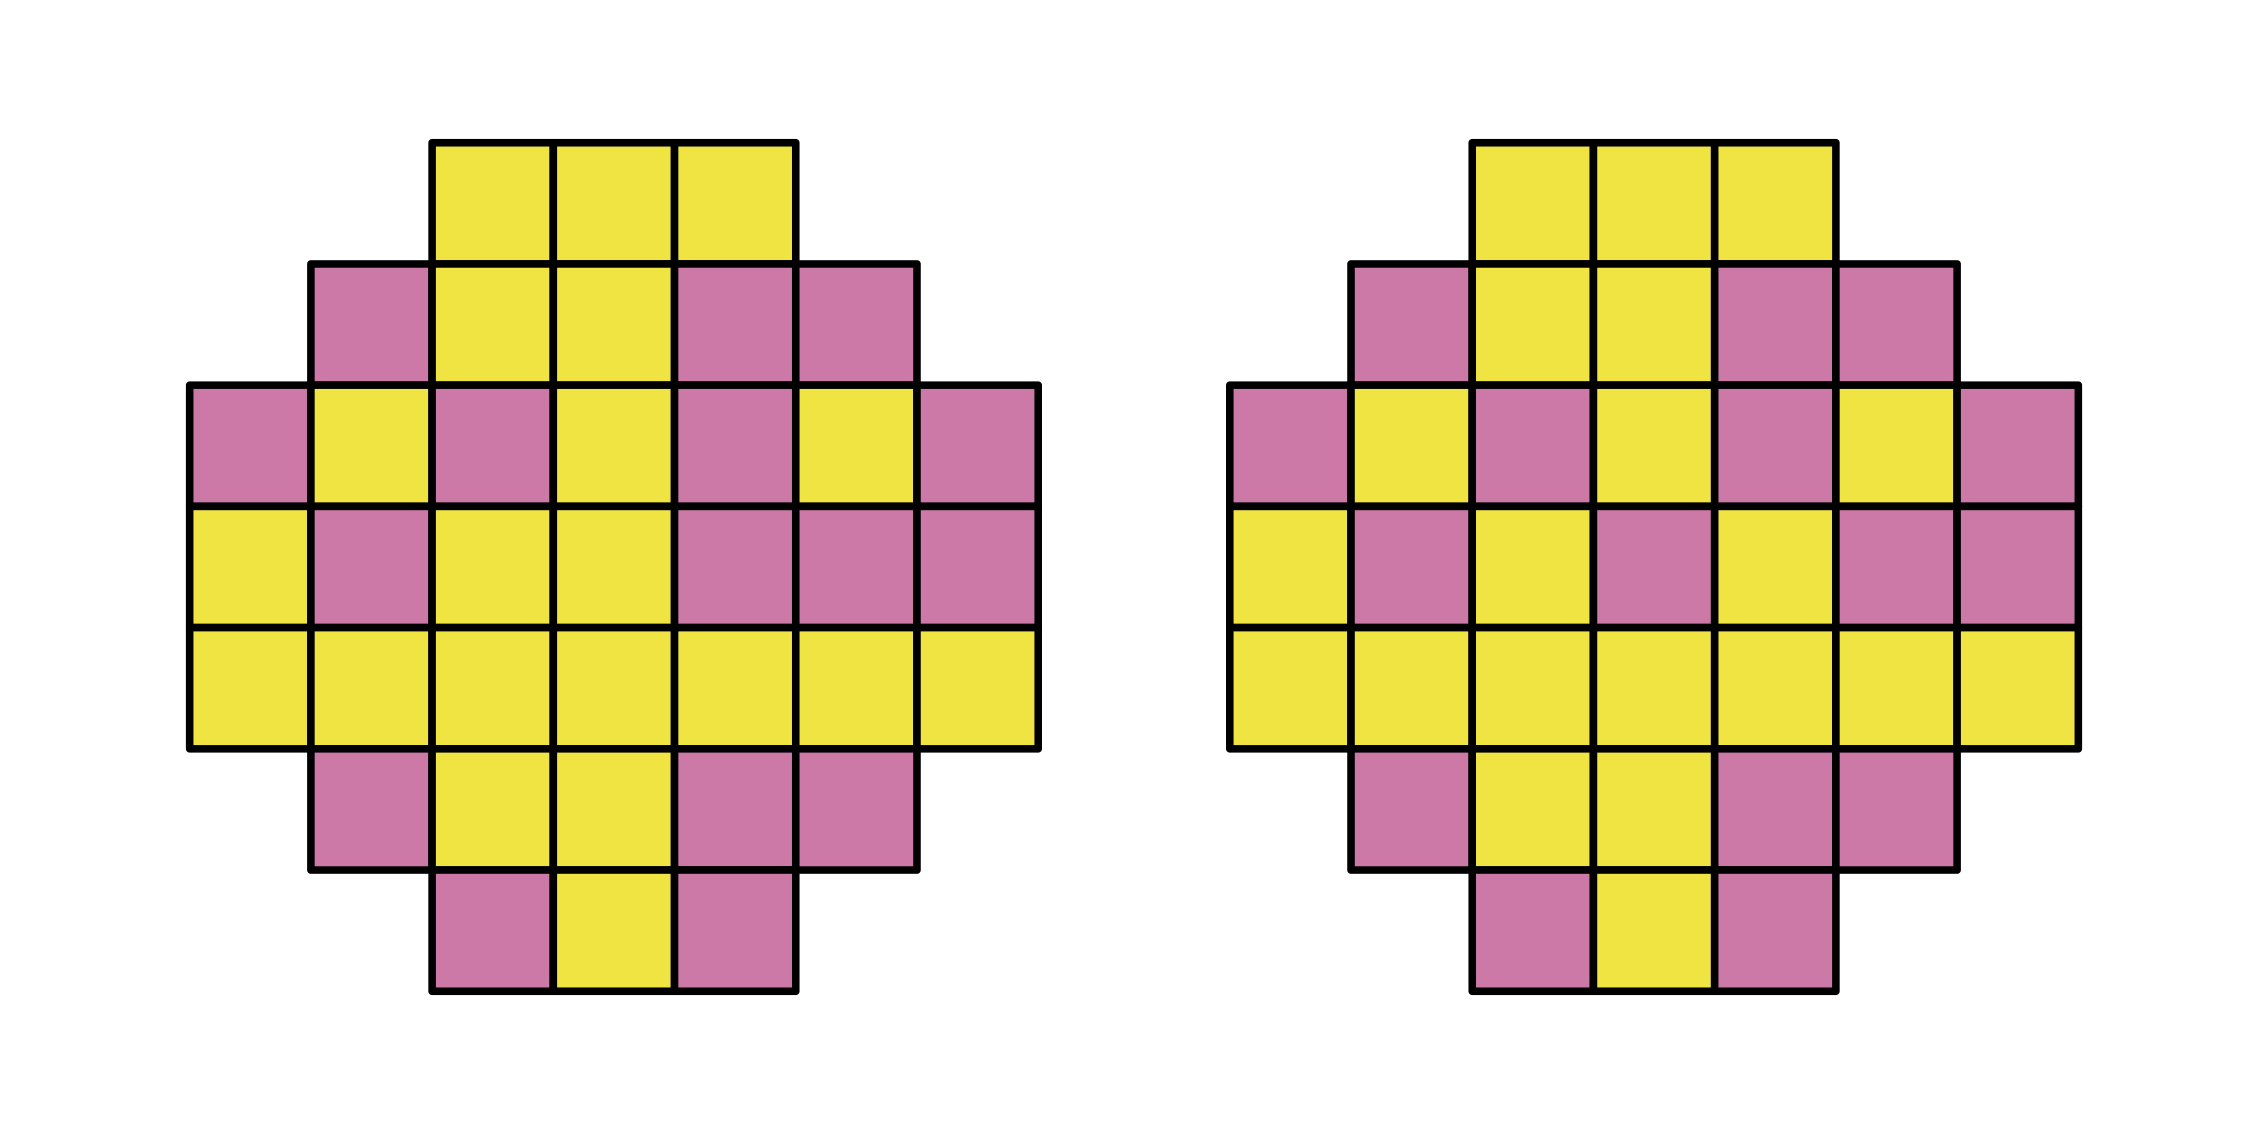
\includegraphics[width=\textwidth]{Figure 11.7.E}
\caption{Two very similar states $g_i$ and $g_j$ differ by two rotated cells near the center, resulting in a convolution score less than $1$}
\end{figure} \noindent
\noindent % An example of a radially symmetric macroparticle region with small Boolean interior defects
If we intend that $G$ represent a class of states that are stable over some period of time, then defective interiors may cause instability that lead to particle dissociation or decryption. If defects or flaws are not corrected soon, then it will dissociate unless by chance vacuum fluctuations or external forces correct the interior to be self-reinforcing. I liken the problem to the \textit{radius of convergence} of a iterative algorithm $(f \circ f \circ . . . \circ f)$.

With our knowledge of defective interiors, let us redefine our terms:
$$\mu_i(x, t) = f(x, t) * \tilde g_i(x)$$
$$\omega_i(x, t) = \omega_i^+(x, t) - \omega_i^-(x,t)$$
\[\omega_i^+(x, t) =
\begin{cases}
1, \quad \mu_i(x, t) = +1 \\
0, \quad \textnormal{else}
\end{cases}
\]
\[\omega_i^-(x, t) =
\begin{cases}
1, \quad \mu_i(x, t) = -1 \\
0, \quad \textnormal{else}
\end{cases}\]
We call $\mu_i$ the \textit{raw measure} of $\tilde g_i * f$. We call $\omega_i$ the strict frequency of $\tilde g_i$ in $f$, $\omega_i^+$ the strict frequency of positive variants of $\tilde g_i$ in $f$, and $\omega_i^-$ the strict frequency of negative variants of $\tilde g_i$ in $f$. 

This allows us to simplify counts over the whole class $G$ as a maximum function:
$$\omega(x, t) = \underset{k \in 1,...,\theta_G}{\max} \omega_k(x,t)$$
in which $\omega(x, t)$ is the strict frequency of $G$ in $f$ and $\theta_G$ is the number of states in class $G$. This measures if there is a normalized state in $G$ that perfectly matches a portion of $f$ for each cell $(x, t)$. We say that $\omega(x, t)$ is an element of the set $\{-1, 0, +1\}$ such that it counts the antiparticle presence, null presence, and particle presence of $G$ in $f(x, t)$.

Remember that we are often working with a stochastic transition matrix $P$ representation of our system. If we determine some $\omega(x)$ measure for each Boolean configuration eigenstate $\hat X$ of the state space $\mathcal X$, then we can track the creation and annihilation of particles in a stochastic matrix $P$. Let $\Omega^+$ and $\Omega^-$ be the sum of particles and antiparticles present in some configuration eigenstate $\hat X$:
$$\Omega^+ = \sum\limits_{x \in X} \omega^+(x), \quad \Omega^- = \sum\limits_{x \in X} \omega^-(x)$$
We may say that $\Omega^+$ and $\Omega^-$ are measures just like $\mathcal X$ with respect to stochastic transition matrix $P$ such that:
$$(\Delta \Omega^+)_{(i, j)} = \Omega^+_{\hat X_j} - \Omega^+_{\hat X_i}$$
$$(\Delta \Omega^-)_{(i, j)} = \Omega^-_{\hat X_j} - \Omega^-_{\hat X_i}$$
These are two-dimensional measures of particle creation/annihilation and antiparticle creation/annihilation respectively. For example, we may wish to measure the average number of particles created/annihilated at a time step $t$ via the expectation:
$$\langle \Delta \Omega^+ \rangle_t = (y_0 (P^t \odot \Delta \Omega^+)) \cdot \textbf{1}$$

Let us posit a hypothetical state space graph representing particle creation/annihilation:
\begin{figure}[H]
\centering
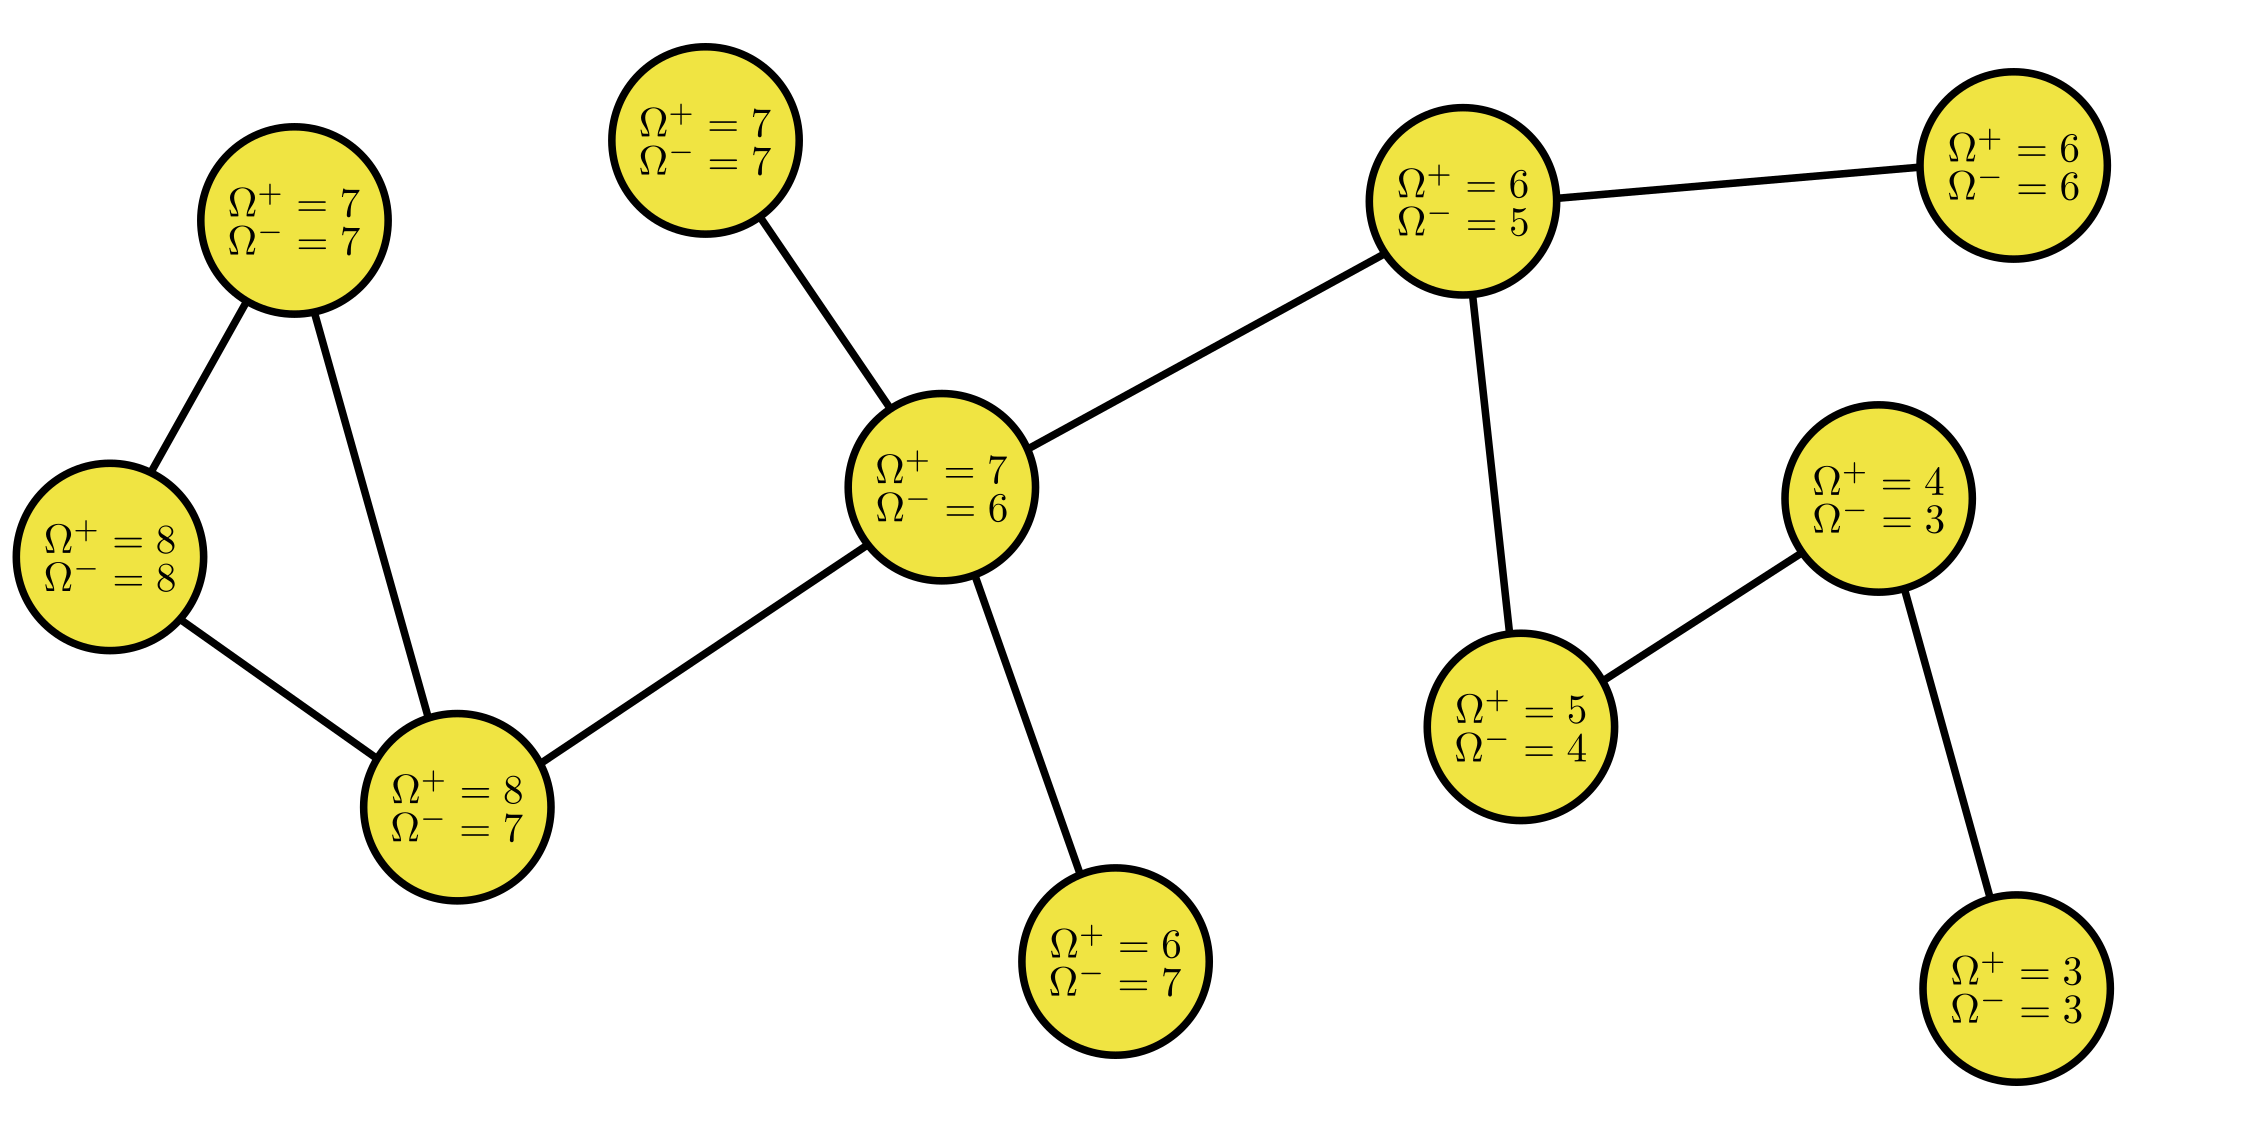
\includegraphics[width=\textwidth]{Figure 11.7.F}
\caption{A state space graph of a system biased towards positive counts of a particle}
\end{figure} \noindent
\noindent % Four configuration eigenstates with differing particle counts each
This take toy example graph allows us to exactly analytically identify particle creation and annihilation as transitions, but there is still subjectivity of what states $g$ we consider to be part of a macroparticle class $G$. 

\part{Boolean Mechanics Philosophy}

\chapter{Daoist and Kantian Philosophy}
Daoism is a diverse class of philosophies and traditions that originate from China. It seeks to describe the way the universe works and how to live a life that is in harmony with it. Daosim is not so singular or unified as the monotheistic traditions. Dao literally means way, path, or road. It may be interpreted as the impersonal cosmic flow of reality. Daoism does not have a defined canon of scriptures because it emphasizes that there are many valid ways or sources of interpreting the universe. Daoism evades rigid classification.

Kantian philosophy refers to the philosophy of transcendental idealism founded by Immanuel Kant in Germany in his book \textit{Critique of Pure Reason}. His work emphasizes the separation between \textit{noumena}, objects that exist independently of the sense, and \textit{phenomena}, objects whose existence is derived from the senses. Kant argues that the human mind has \textit{a priori} (or before experience) knowledge of time and space, arguing what we \textit{can} sense and how that that input is structured directly influences our experience of reality. Our model of reality is the continuous dialogue of rationalism and empiricism. Rationalism emphasizes that knowledge of the world is best assumed top-down via logical conclusion. Empiricism emphasizes that knowledge of the world is best understood bottom-up via undeniable evidence. Kantianism emphasizes rigid classification.

Eastern philosophy and Western philosophy inherit their tradition from these schools of thought due to differences in their geography. In East Asia, the humble rivers born from rigid mountains could not be bent by human will, and fate decided communities must be established by the rivers that would carry trade and commerce between them. Eastern heroes frustrated with the flow of the universe travel up to the mountain tops in isolation, and there in their solitude do they become at peace with the things they cannot change. Confucianism emphasizes harmony with the social world after mastery while Daoism emphasizes harmony with the natural world.

How does this contrast to Western points of view? In the colonized West, the great waves of chaos and strife may be tamed by a great captain leading his crew, and the sheer force of human skill and will may determine who safely makes it to shore carrying riches of the new world. Western heroes challenged by nature or enemies band together to go on an adventure far from home, and there in their camaraderie do they gain the skills and confidence that they can change the way things are to earn peace. The skills learned from rationalism and empiricism are intended to expand one's influence over reality, be it the natural world or social world.

Is peace found internally alone through great reflection or is it fought for externally together through great triumph? The choice to master the internal world or the external world is up to the individual. Is learning the social world or natural world more important? It depends on the time and place as well as the goal of the individual, but I would argue that the humanities have been oft neglected in favor of the sciences.
\begin{center}
\begin{tabular}{| c | c | c |}
\hline
\textit{} & Internal & External \\
\hline
Natural & Formal Science & Natural Science \\
\hline
Social & Humanities & Social Science \\
\hline
\end{tabular}
\end{center}
The neglect of the humanities has created a void in which we use our understanding of the natural world, internal and external, in order to socially dominate others. Weakened cultural appraisal of the humanities results in book burning, media censorship, and the rise of tyrannical actors. Weapons of war are increasingly favored over weapons of rhetoric in order to maintain the ``security'' of states in power.

In order to fix the problems of the state, a greater emphasis of humanities education needs to exist at the primary, secondary, and tertiary level. This is not a theoretical argument: all the formal sciences and some of the natural sciences that deal with the theoretical foundations of mathematics and physics are eschewed in favor of ``immediate returns''. The natural sciences with which our technology relies upon to achieve dominance in the social world depends on developments in the formal sciences. Anti-intellectual sentiment against the humanities increasingly targets the formal sciences, a crude sort of self-mutilation as most of our comfort in the modern world was due to pointless ideas.


\section{Patterns of Value in Time and Space}
Daoist philosophy dictates that the material world must be composed of two irreducible substances, yin and yang, in order to make a distinguishable reality. Distinguishability originates from temporal and spatial differences in value, and specific arrangements that occur frequently are important patterns. Yin and yang are not merely opposites but complements that cannot be negated. It is the flow of their attraction and inseparability that creates a dynamic and cyclic system that is more complex than its individual parts. Paint that never mixes.

\textbf{Yin and yang}\index{yin and yang} are polar or binary components of a system, \textit{yin} (陰) referring to the shaded side of a hill while \textit{yang} (陽) refers to the illuminated side. Together they form the \textbf{taiji} (太極), literally meaning maximum polarity (tai 太: great, supreme; ji 極: pole, extremity). This is in contrast to \textbf{wuji} (無極), which means without limit, infinity, or non-polar. Without differences in value in time and space, \textit{things would cease to exist}. In a literal sense, an object \textit{objects} to complete communication through its inhabited space as defined by its boundary. In an abstract sense, this is due to the limits of the communicability or information rate of that space.\footnote{Limitations are due to signal type or Shannon's limit of channel capacity.}

Kantian philosophy proposes that the human mind comes pre-equipped with the faculties to comprehend time and space. I ask first and foremost: \textit{what are you measuring} with respect to \textit{time} and \textit{space}? Time and space are only useful constructs with respect to some minimal measurement basis: the Boolean set $\mathbb B_\pm = \{ -1, +1 \}$, also known as yin and yang. In fact, time and space are higher-order constructs of value when we represent a simulation on a computer using bits. Even the word \textit{simulation} implies that some value is changing in time and space. It is not time nor space that changes in a simulation, but their representation via Boolean values. On a computer, a $0$-dimensional array is a scalar, and the minimum discrete scalar of $2$ demands the Boolean set $\mathbb B$.

\section{Ordinality of Value, Time, and Space}
How can we be certain that patterns of value in a snapshot of time and space are what define reality? Would such a theory be compatible with mainstream theories in physics? Consider the following $2$-space, $1$-time array constructed using elements from the set $\{0\}$:
\begin{figure}[H]
\centering
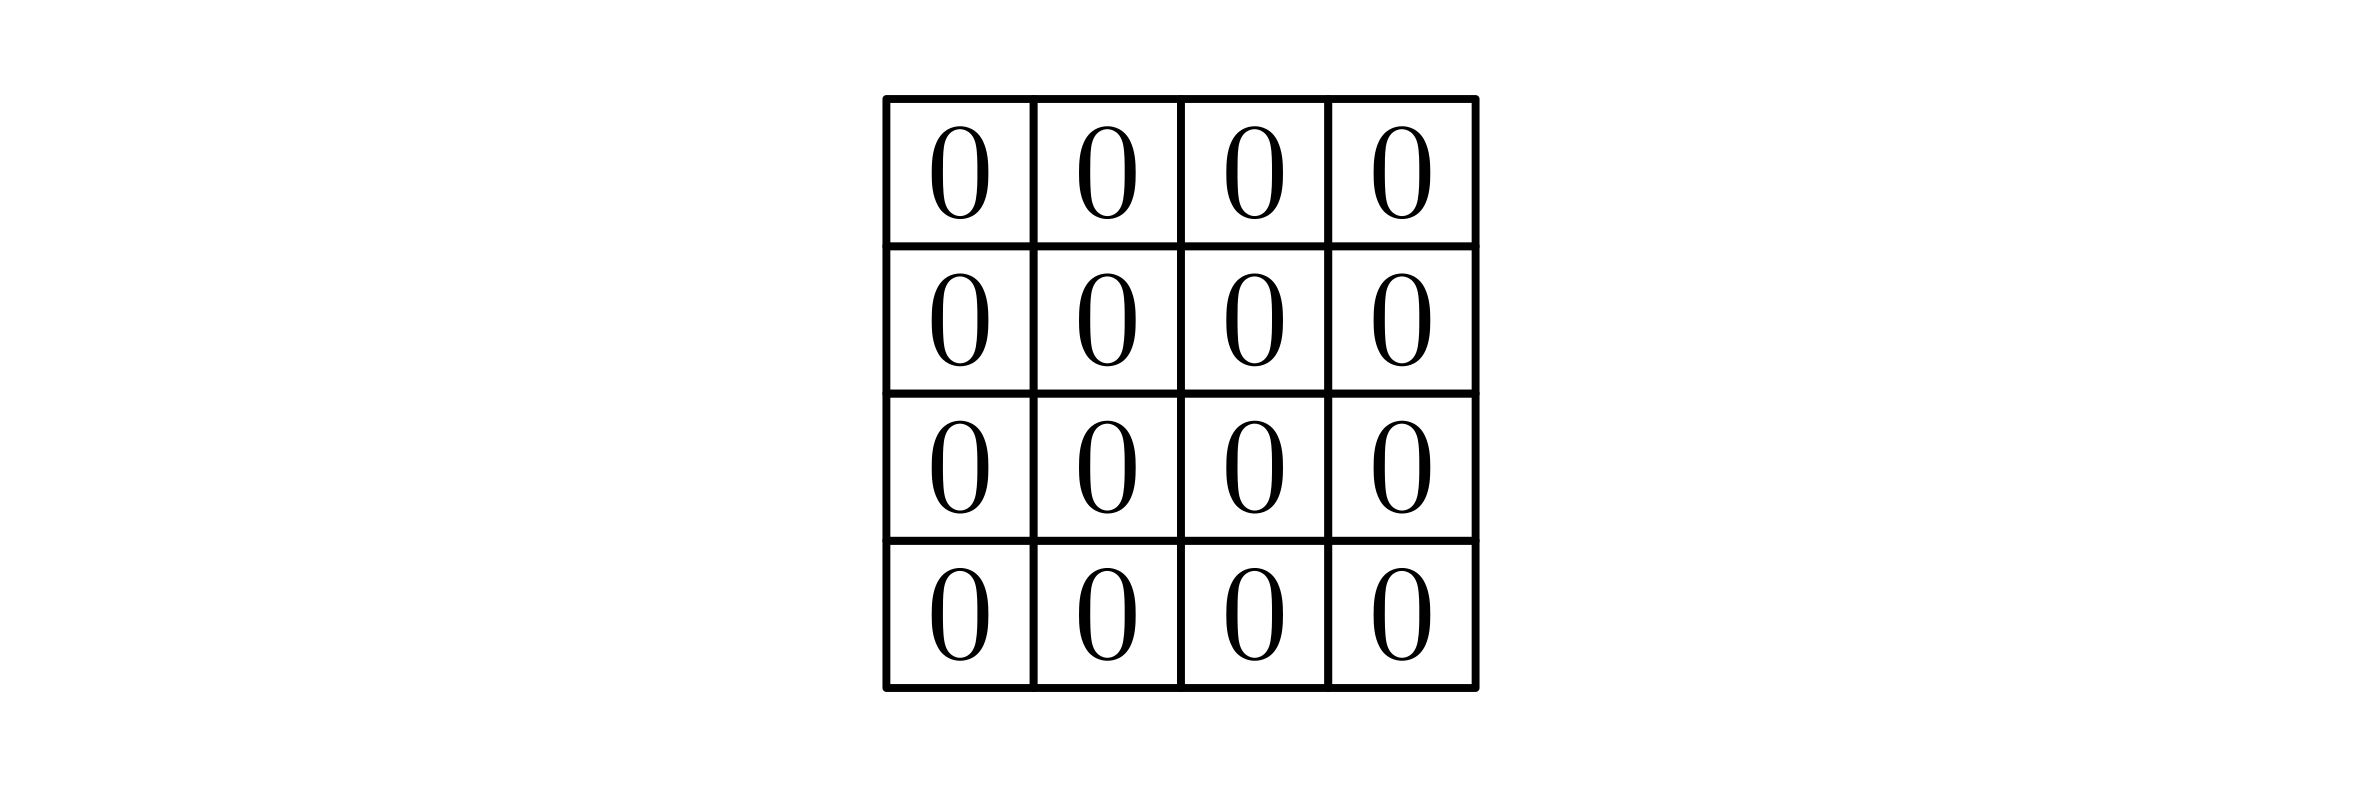
\includegraphics[width=\textwidth]{Figure 13.1.A}
\caption{An array of information units with cardinality $1$, lacking uniqueness in pattern}
\end{figure} \noindent
\noindent % An 2D array of 0s stacked along a 1D array of time
Even if we were to extend time and space infinitely, any measuring function we apply to time and space that can only use elements from a set with a single element cannot generate a distinguishable reality.

Now that we presume that value precedes time and space necessarily, is time or space more important at a metaphysical level? Consider a sensor that reads the salinity of soil, and it does this by measuring the conductivity between two electrodes:
\begin{figure}[H]
\centering
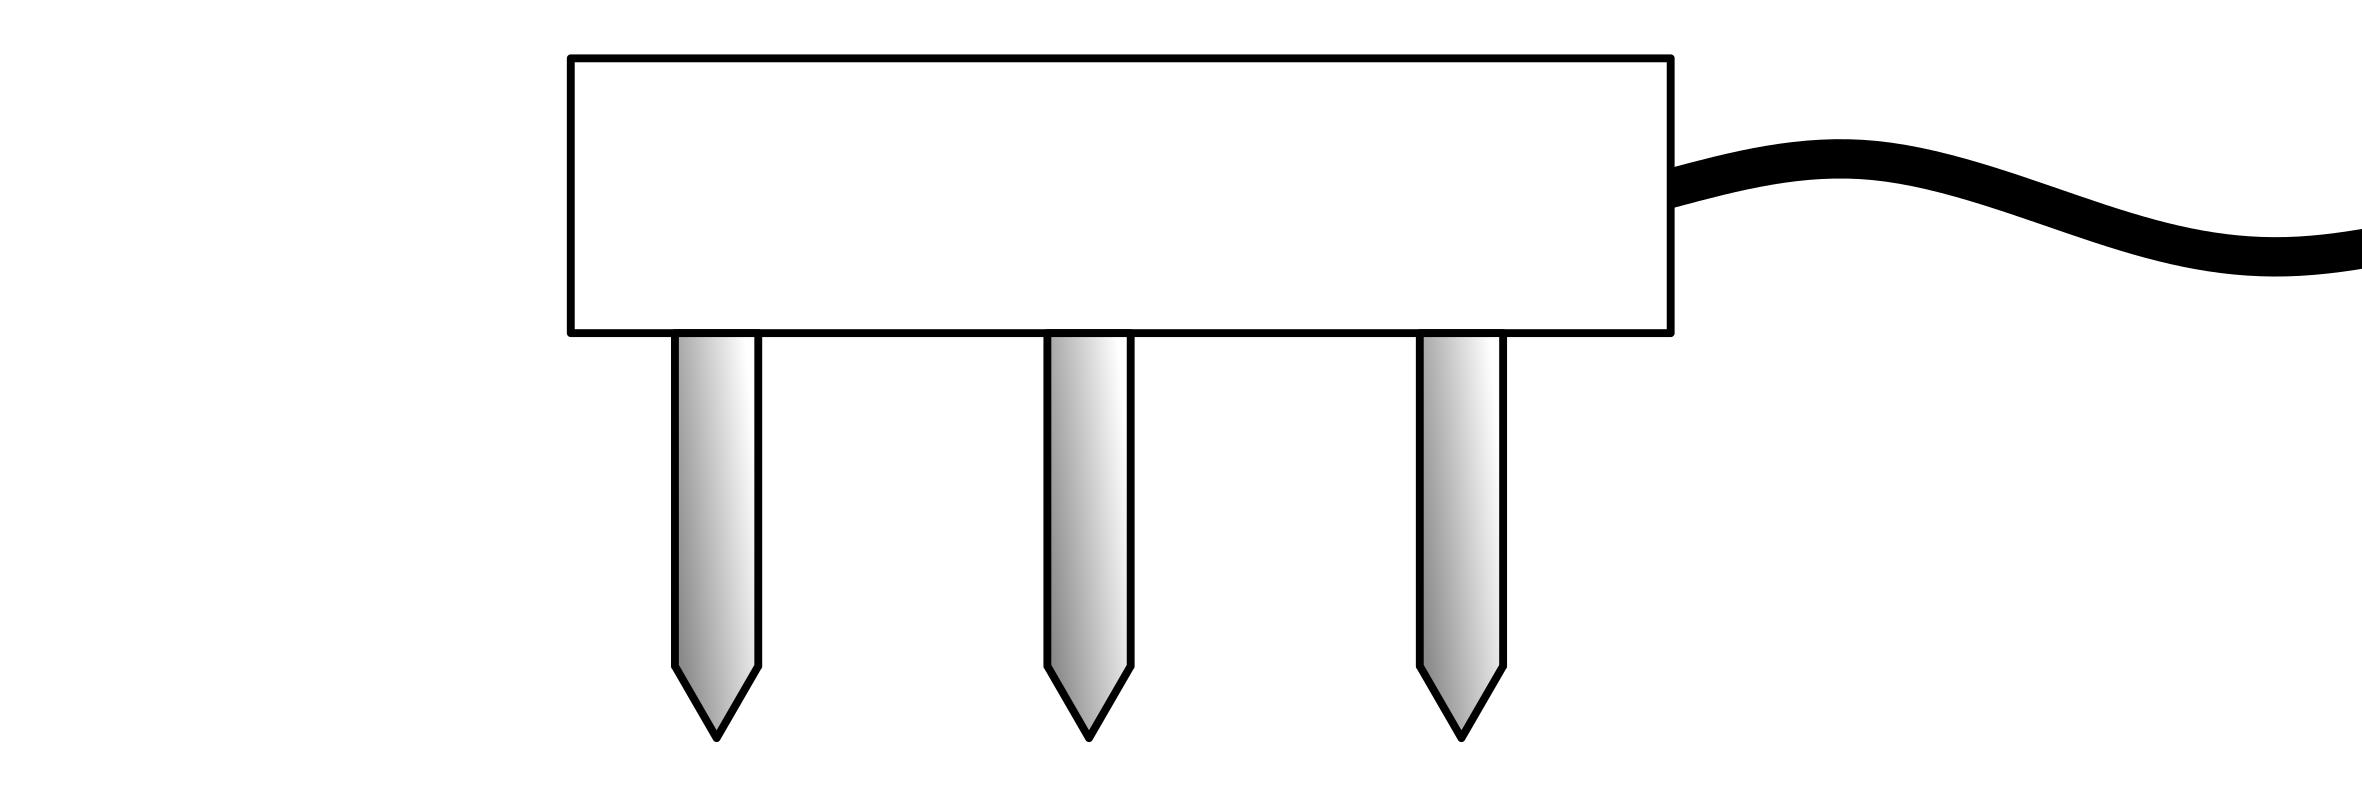
\includegraphics[width=\textwidth]{Figure 13.1.B}
\caption{A soil salinity sensor measures electrical conductivity across steel probes}
\end{figure} \noindent
\noindent % Image of an electrode in soil
This device is akin to the primitive sensor of a biological organism. While at first glance the object is measuring a piece of data along space, the organism is actually recording the data stream with respect to time. A single sensor is insufficient to measure values across space, and an inaccurate model of space is less likely to kill an organism than an inaccurate model of time. The electricity generated from a microphone that vibrates across space is likewise measuring changes in a value across time. Even photos, which measure snapshots of space, are used to remember ``good times''. Quite the linguistic paradox, wouldn't you agree?

Perhaps the argument I make is too anthropocentric and not principled enough, but living things are more concerned with surviving into the future by predicting it. Predicting the future is arguably more important to an organism than predicting what may be over a hill, behind some barrier, or concealed behind fog.

\section{Paradox of Impermanence and Inevitability}
A probability is a possibility. A possibility is an eventuality. The paradox of living things is that they must replicate themselves across time and space in order to not die, but they must also partially die by changing in order to live. Without adaptation, the world shall change around them regardless. In order for you to navigate treacherous terrain, you must kill the ideas that may kill you. Changing your mind and letting go is difficult because some ideas refuse to die: Ideas may generate their own survival defense mechanisms. Faith is a brain worm just as much as music.

In order for every computable function to be inevitably computed, every computationally stable or self-computing structure must be impermanent or have a finite lifetime. Likewise, if something dies, then it is guaranteed to return. Every state and substate of a Boolean mechanical system is recurrent no matter the size or dimension.\footnote{The metaphysical consequences of the second Borel-Cantelli lemma are far reaching.} Though lone random walkers in 3D may never return to their origin, that does not mean that a specific Boolean pattern is gone forever. It is the pattern, not the individual particles and antiparticles themselves, that are guaranteed to recur in an infinite-time, infinite-space simulation. Every deck of cards shall be played. Similar to ``The Egg'' by Andrew Weir, you and I shall become each other in time as well as every hero and villain.

It is unlikely that Boolean random walks is the true way of the universe's flow, but that matters little. The core principles will carry over to whatever is the correct transition function, assuming there is one to be found. Under the framework of stochastic cellular automata, particles of quantum mechanics do not really \textit{exist} in the sense of noumena. Instead, the things we call particles are the result of computable spaces that have the \textit{property of behaving like particles}. I phrase it like so because the patterns that generate particle-like behavior from the Big Bang have likely existed before the Big Bang, but there was a lack of \textit{support structure} for them to persist. For example, the genetic code of a human is not sufficient for birth. It requires the context and support of a mother's womb in order to function properly. Similarly, a Boltzmann brain, a human brain that exists because of random fluctuations in the universe, would be infrequent due lack the support structure to maintain the experience of consciousness.

This begs the question: What are the general properties that make the universe possible? The simplest informal answer I have is random, recurrent, and non-uniform non-independence. The transitions are random, the states are recurrent, and the particles/cells interact non-uniformly due to statistical dependence to other cells. Transitions of value across time and space that obey these rules can be expected to compute anything, eventually everything, if given enough time. The question is whether we need continuity or if discrete structures are sufficient to generate reality.

The emergence of higher-order structures depends on something more fundamental. There is something essential that must be described that is more general than a Boolean mechanical system. Hence, I describe the basics of computational information systems.

\section{Computational Information System States}
A \textbf{computational information system}\index{computational information system} is a universe with a set of rules that give it the ability to:
\begin{enumerate}
\item represent
\item process
\item prefer
\end{enumerate}
information states. These vague terms in plain language are intentional. There are many possible sets of rules that generate a universe that will fulfill these requirements and infinitely many more that will not. This set of rules should avoid Russell's paradox involving the set of all sets discussed in \textit{\S 1.2 Sets and Operators}. What are the minimal rules that will fulfill these requirements? What even is an information state?

An information state $X$ is a finite composition of information units $x$ assigned a measuring probability function $\mu$:
$$X = x_1 \times x_2 \times ... \times x_N = \prod\limits^{N}_{i=1} x_i$$
The $2$-tuple $(x, \sigma)$ is called a \textbf{measurable unit}\index{measurable unit} in which little $x$ is a set and little $\sigma$ is its $\sigma$-algebra. To define a \textbf{probability measure}\index{probability measure} $\mu$, we require the following properties:
\begin{enumerate}
\item Normal Measure: $\mu(\varnothing) = 0, \ \mu(\varepsilon) = 1$ if $\varepsilon = x$
\item Partial Measure: $\mu (\varepsilon) \geq 0, \ \forall \varepsilon \in \sigma$
\item Disjoint Measure: $\mu \Big ( \bigcup\limits^{n}_{i=1} \varepsilon_i \Big )= \sum\limits^{n}_{i=1} \mu(\varepsilon_i)$, for disjoint sets $\varepsilon_i$
\end{enumerate}
The $3$-tuple $(x, \sigma, \mu)$ is called a \textbf{unit probability measure}\index{unit probability measure}.

The $2$-tuple $(X, \Sigma)$ is called a unit of \textbf{measurable state}\index{measurable state} or measurable composition in which $X$ is the Cartesian product of $N$ measurable units $x$ and $\Sigma$ is the product $\sigma$-algebra:
$$\Sigma = \sigma_1 \times \sigma_2 \times ... \times \sigma_N = \prod\limits^{N}_{i=1} \sigma_i$$
To define a \textbf{probability measure}\index{probability measure} $\mu$, we require the following properties:
\begin{enumerate}
\item Normal Measure: $\mu(\varnothing) = 0, \ \mu(E) = 1$ if $E = X$
\item Partial Measure: $\mu (E) \geq 0, \ \forall E \in \Sigma, \ E = \prod\limits^{N}_{i=1} \varepsilon_i$
\item Disjoint Measure: $\mu \Big ( \bigcup\limits^{n}_{i=1} E_i \Big ) = \sum\limits^{n}_{i=1} \mu(E_i)$ for disjoint sets $E_i$
\item Zero Measure:$\mu (\varepsilon_1 \times \varepsilon_2 \times ... \times \varepsilon_N) = 0$, \ if $\varepsilon_k = \varnothing, \ \mu(\varepsilon_k) = 0$
\item Unconditioned Measure: $\mu(\varepsilon_1 \times ... \times \varepsilon_N) = \mu(\varepsilon_1 \times ... \times \varepsilon_{k-1} \times \varepsilon_{k+1} \times ... \times \varepsilon_N)$, if $\varepsilon_k = x$
\item Conditioned Measure: $\mu(\varepsilon_i \times \varepsilon_j) = \mu(\varepsilon_i | \varepsilon_j)\mu(\varepsilon_j)$ $= \mu(\varepsilon_j | \varepsilon_i)\mu(\varepsilon_i)$
\item Definitely Measurable: Any $E$ is definite if $\varepsilon_i \neq \varnothing$ for all $\varepsilon_i \in \sigma_i$ and for all $i \in {1,...,N}$
\item Uniquely Measurable: Any $E$ is unique if $\varepsilon_i \in x$ for all $\varepsilon_i \in \sigma_i$ and for all $i \in {1,...,N}$. A unique $E$ is denoted as $\hat X$, and the set of all unique configurations $\hat X_1,..., \hat X_\theta$ are disjoint.
\item Non-trivially Measurable: Any $E$ is non-trivial if $\varepsilon_i \neq \varnothing, x$ for all $\varepsilon_i \in \sigma_i$ and for all $i \in {1,...,N}$
\item Separably Measurable: Any $E$ is separable into unique information states $\hat X_1 ,..., \hat X_n$ if $E$ is non-trivial but not unique. Its measure is the sum of these unique configurations, $\mu(E) = \sum\limits^{n}_{i=1} \mu(\hat X_i)$.
\end{enumerate}
These properties help create a well-defined information system for any point in time. Though information units $x$ are identical, they are not necessarily statistically independent.

We call the state space $\mathcal X$ the set of all unique information states $\mathcal X = \{ \hat X_1, \hat X_2, ..., \hat X_\theta \}$ such that:
$$ \mu \bigg ( \bigcup\limits_{S \subset \mathcal X} \hat X_i \bigg ) = \sum\limits_{S \subset \mathcal X} \mu ( \hat X_i )$$
represents that any probability measure of the union of unique information states is the sum of the measures of unique information states. To reiterate, the set of unique information states of a probability measure are necessarily disjoint. As a reminder, each unique configuration $\hat X$ is the result of each information unit $x$ choosing a single element from the defining information set $x$:
$$\hat X = \prod\limits^{N}_{i=1} x_i, \quad x_i \in x$$
We call the $3$-tuple $(X, \Sigma, \mu)$ a \textbf{product probability measure}\index{product probability space}. 

Each $\hat X$ is not a singleton in the usual definition for $\sigma$-algebras: We consider them \index{product singleton}\textbf{product singletons} or composition singletons. A product $\sigma$-algebra is denoted a $\Sigma$-algebra. If the $\Sigma$-algebra lacks the state space $\{ \hat X_1, \hat X_2, ..., \hat X_\theta \}$ as an element, then at least two of the product singletons in $\Sigma$ share the same \textit{class} as another.\footnote{Two objects which are computationally indistinguishable share the same class. As classification schemes become more refined, they better differentiate components of a class. An academic example is the separation of natural philosophy into philosophy and natural science.}

A computational information system may only ever be in a unique information state from the state space, or rather the probability that it is in one of these unique configuration in the state space is $1$. If the cardinality $|x| = 2$, then every element in the set of every non-trivial compositions of $x$ is unique. If the cardinality of $x$ is any smaller natural number such as $0$ or $1$, then we do not have non-trivial compositions. If the cardinality of $x$ is a larger natural number value such as $3$ or $4$, then there are non-trivial compositions that are not unique. 

In the case of larger $|x| > 2$, we must utilize the additive property combined with the unconditioned property to properly measure it by parts. Suppose $x = \{a, b, c\}$ and $X = (x_1, x_2)$, thus each little $\sigma$-algebra is:
$$\sigma = \{\varnothing, \{a\}, \{b\}, \{c\}, \{a, b\}, \{b,c\}, \{a, c\}, \{a, b, c\}\}$$
In order to measure $\mu(\{a\}_1 \times \{b, c\}_2)$, we must add the unique states:
$$\mu(\{a\}_1 \times \{b, c\}_2) = \mu(\{a\}_1 \times \{b\}_2) + \mu(\{a\}_1 \times \{c\}_2)$$
Our definition of computational information systems for when the number of information units is countably infinite, $N = \aleph_0$, utilizes \textbf{Zermelo–Fraenkel Choice}\index{Zermelo Fraenkel Choice} (ZFC) as our axioms of set theory.

Suppose that $x = \{0, 1\}$ and $x^{\aleph_0}$ approximates the continuous interval $[0, 1]$. We let $X = [0 ,1]$ encode the set of possible positions for an electron in a one-dimensional box. The set $X$ is \textit{constructed} from units $x$ via the \textbf{axiom of constructibility}\index{axiom of constructibility}, which implies the \textbf{axiom of choice}\index{axiom of choice} and the \textbf{generalized continuum hypothesis}\index{generalized continuum hypothesis} $2^{\aleph_\alpha} = \aleph_{\alpha+1}$ under Zermelo-Fraenkel set theory without the axiom of choice initially included. Consider the probability function of position $p(x)$ in which $p(x,t)$ denotes time advancements since time $0$, $p(x) = p(x, 0)$. A probability distribution upon space requires the axiom of choice, and this evolution of $p$ with respect to well-ordered time also requires axiom of choice. In fact, a probability update of a Wiener process (Brownian motion) requires the \textbf{axiom of global choice}\index{axiom of global choice}. The axiom of constructibility implies the axiom of global choice, which itself implies axiom of choice.

Why be so pedantic about the philosophy of mathematics that will dictate our axioms? We live in a seemingly continuous universe that we desire to obey the discrete laws of computation. If we are to truly understand how the universe works, we need a model that accounts for all the possible ways that a computable universe might emerge. If we are to assume that the universe is understandable and may be learned, it is reasonable to assume that we can construct a model from basic parts. A constructible universe under the axiom of constructibility means that if $E$ is non-trivial, then $0 < p(E) <1$ implies that a construction $E$ in formal mathematics exists if it is computable (may be mapped to a computable number). The mathematical objects that may exist in a mind are strictly computable structures.

The natural choice is to assume that the universe is laid out in a cubic lattice, such as the $d$-dimensional integer lattice of $\mathbb Z^d$. Suppose that we attach an information unit $x$ to each lattice point of $\mathbb Z^d$. If we are using the axiom of constructibility, then deciding upon an information unit of $x = [0, 1]$ is not minimal since the set $[0, 1]$ may be constructed using the set $\{0, 1\}$. Likewise, a continuous interval of space using axiom of constructibility would not be necessary under that same principle. Each lattice point's infinite past is sufficient to endow it with the continuity as given by the generalized continuum hypothesis $2^{\aleph_\alpha} = \aleph_{\alpha+1}$ as implied by the axiom of constructibility.

A continuous theory of physics would need to be minimal in an axiomatic set theory that is stricter than Zermelo-Fraenkel Choice but less strict than Zermelo-Fraenkel Constructibility. We shall refer to Zermelo-Fraenkel Constructibility as ZFC$\times$ in which the multiplication symbol $\times$ refers to the Cartesian Product. In physics, the direct sum symbol $\oplus$ is equivalent to the Cartesian product for finite direct sum of $x$:
$$\prod\limits_{i=1}^N x_i = \bigoplus\limits_{i=1}^N x_i, \quad N < \infty$$
Thus, we shall call this continuous theory's axioms as ZFC$\oplus$ (or ZFC+ in plain text). I am unsure how such a theory would handle time and length scales smaller than Planck units. Consider the direct sum of $N$ units of $x$:
$$\bigoplus\limits_{i=1}^N x_i, \quad |x| = \aleph_{0} $$
in which $x$ is an infinitely countable set of orthonormal basis vectors called a \textbf{Hilbert space}\index{Hilbert space}. Since the basis vectors for $x$ is countable and each $x_i$ is unique, we have a separable $\sigma$-algebra even if our space is continuous (as compared to the Boolean statistical mechanics preference for $N$ discrete units of identical $x$). The value of using a direct sum over a Cartesian product is that an infinite direct sum of a Hilbert space gives $0$ measure almost everywhere except for a countably finite number of terms.

The main issue I foresee is that there is no natural orthonormal basis to choose for $x$, and the other issue is that the differential equations that guide real physics are not as scale-invariant as the math suggests.\footnote{The first issue is forgivable as there is no natural transition function to consider for Boolean statistical mechanics. The second issue is rectified by discrete mechanics, which are obviously not scale-invariant.} Suppose that we choose an Hilbert basis for $x$ which contains representations of the occupancy number of a particle:
\begin{enumerate}
\item[$0:$] $| 0, 0, 0, 0, ...\rangle $
\item[$1:$] $| 1, 0, 0, 0, ...\rangle, \ | 0, 1, 0, 0, ...\rangle, \ | 0, 0, 1, 0, ...\rangle, ... $
\item[$2:$] $| 1, 1, 0, 0, ...\rangle, \ | 0, 1, 1, 0, ...\rangle, \ | 1, 0, 1, 0, ...\rangle, ... $
\end{enumerate}
The zero state represents the vacuum. Each state that corresponds to an occupancy number called a \textbf{Fock state}\index{Fock state} or \textbf{number state}\index{number state}. The time evolution of any initial system state would need to equilibriate into some probability distribution of these stable solutions. If we are to separate our space into smaller regions, then we must either disallow specific solutions from existing or allow an entire universe to re-emerge within our smaller regions. 

Since physics is not scale-invariant, we cannot allow an entire universe unto itself to exist inside an infinitesimally small region. We must rescale the entropy (or information capacity) of the probability distribution for each region. This is true even if we choose a relatively plain Hilbert basis such as the Fourier basis.

Since we allow for separable regions of space and the zero Fock state, we can have infinitely many regions of space between two existing particles. This is what leads to our information capacity disaster. In quantum field theory, a finite number of particles exist orthogonal to the vacuum as emergent phenomenon of their respect fields. Information in each quantum field travels at most at the speed of light, or the speed of information. Without an inherent scale to vacuum fluctuations in energy, there would be no minimum particle size such that two electrons have an infinite number of infinitesimal electron-positron pairs between them. This is related to the problem of \textit{renormalization} in physics.

These regions with probability measures on their Fock states are obviously not independent of each other. These topological solitons must have a minimum size. The only way for these solitons to be created and annihilated to and from the vacuum state is to have some kind of vacuum fluctuation. Refer back to \textit{\S 11.7 Macroparticle Creation and Annihilation} for more details regarding the formation of solitons in discrete spaces. This leads us back to the problem of deciding upon a natural vacuum noise function and natural partial differential equation for quantum field theory. Such a noise function is problematic if we have a Markov assumption, leading to a continuous everywhere but differentiable nowhere function like the Weierstrass function or a Wiener process.

A proper continuum physics theory needs a definite vacuum noise function that disallows for infinite information between two points (of space or time), that allows particles to be stable under vacuum fluctuations, and allows particles to create or annihilate spontaneously at a fixed size. It is not enough to model wave functions for existing particles if you cannot model how the particle came to exist, at an irreducible size no less. A fundamental scale and maximum amplitude on the noise function means Boolean mechanical system on a rectangular lattice could approximate the continuum with minimal information loss using the appropriate \textbf{Nyquist frequency}\index{Nyquist frequency}, the frequency of a continuous signal that a discrete signal sampler can recreate without aliasing or error.

\textbf{Constructivist mathematics}\index{constructivist mathematics} is strict in a way that ensures that an eigenclass for a random boundary not only implies that macroparticles exist but \textit{guarantees} that they exist. If there is directly an algorithm that can construct the mathematical object with the desired properties, then it exists. Not only that: it exists in a way that can be directly found by a computer or modeled finitely. A Boolean mechanical system that will represent every computable function using local operations is bound to represent them, and living things that leverage local correlations of information will emerge. 

Suppose that $X$ is a large Boolean mechanics simulation from which we sample $\partial G$ for a separate system $G$ as its boundary:
\begin{figure}[H]
\centering
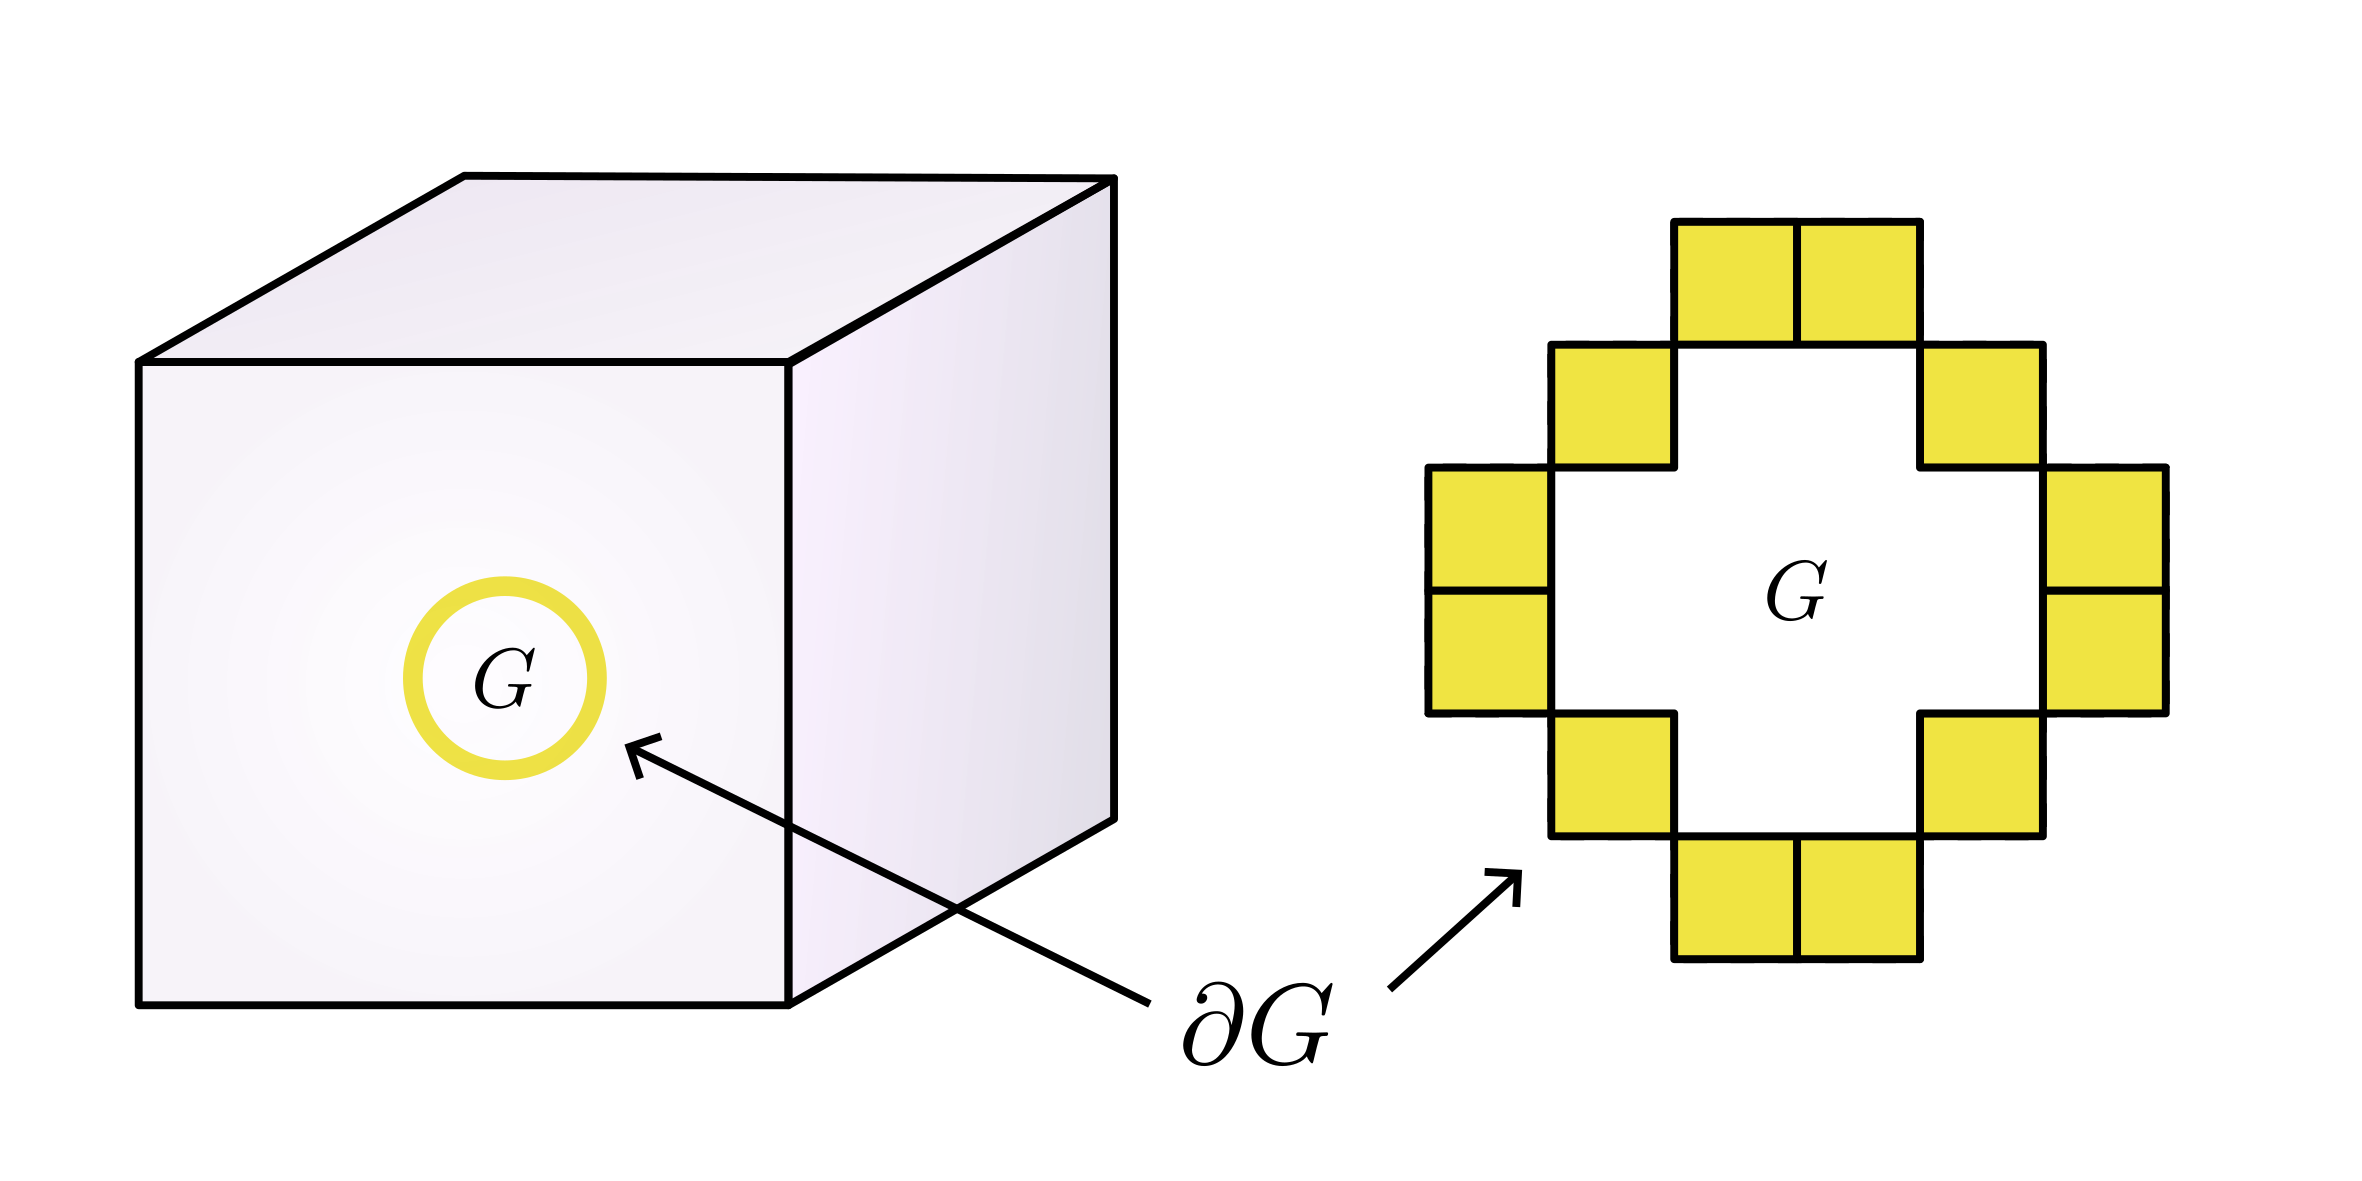
\includegraphics[width=\textwidth]{Figure 13.1.C}
\caption{Sampling conditional $\partial G$ can help identify unique classes for $G$}
\end{figure} \noindent
\noindent % A representation of a boundary sample dG of the region G
If $G$ is a set of states that obey some boundary condition with respect to time evolution, then forcing those boundary conditions will construct the set $G$.\footnote{This method works because any initial condition is constrained to its Markov communication class.} Instead of looking for an interior that fulfills a specific boundary condition, we can coerce a conditional distribution on the boundary and see what interiors it transitions to and from.

Constructive mathematical objects may be reverse engineered using a stochastic process as in the above example because they are explicitly constructed according to some algorithm. A non-constructive proof of an object's existence leaves many degrees of freedom unspecified. In contrast, constructably derived objects guarantee computability and therefore their existence (but not stability or lifetime) in Boolean statistical mechanics.


\section{Computational System Processes}
A \textbf{computational information system}\index{computational information system} is a universe with a set of rules that give it the ability to:
\begin{enumerate}
\item represent
\item process
\item prefer
\end{enumerate}
information states. It works upon our chosen set theory axioms of Zermelo-Fraenkel Constructibility, which we call ZFC$\times$. The \textbf{axiom of constructibility}\index{axiom of constructibility} means that every set is constructible, such as using $\{0, 1\}^N$ to represent the natural numbers $\mathbb N$ as $N \rightarrow \infty$. How does a computational information system transition between states?

Since our information state $X$ is a finite construction of information units $x$ via the Cartesian product:
$$X = \prod\limits_{i=1}^N x_i, \quad x_i \in x$$
it relates itself to any other finite construction (including itself) via a set of allowed \textbf{actions}\index{action}. Finite compositions of these allowed actions generate a \textbf{group}\index{group}. 

The minimal set of allowed actions necessary to generate that group are called \textbf{elementary actions}\index{elementary action}, and we call their finite composition a process $\pi$:
\begin{figure}[H]
\centering
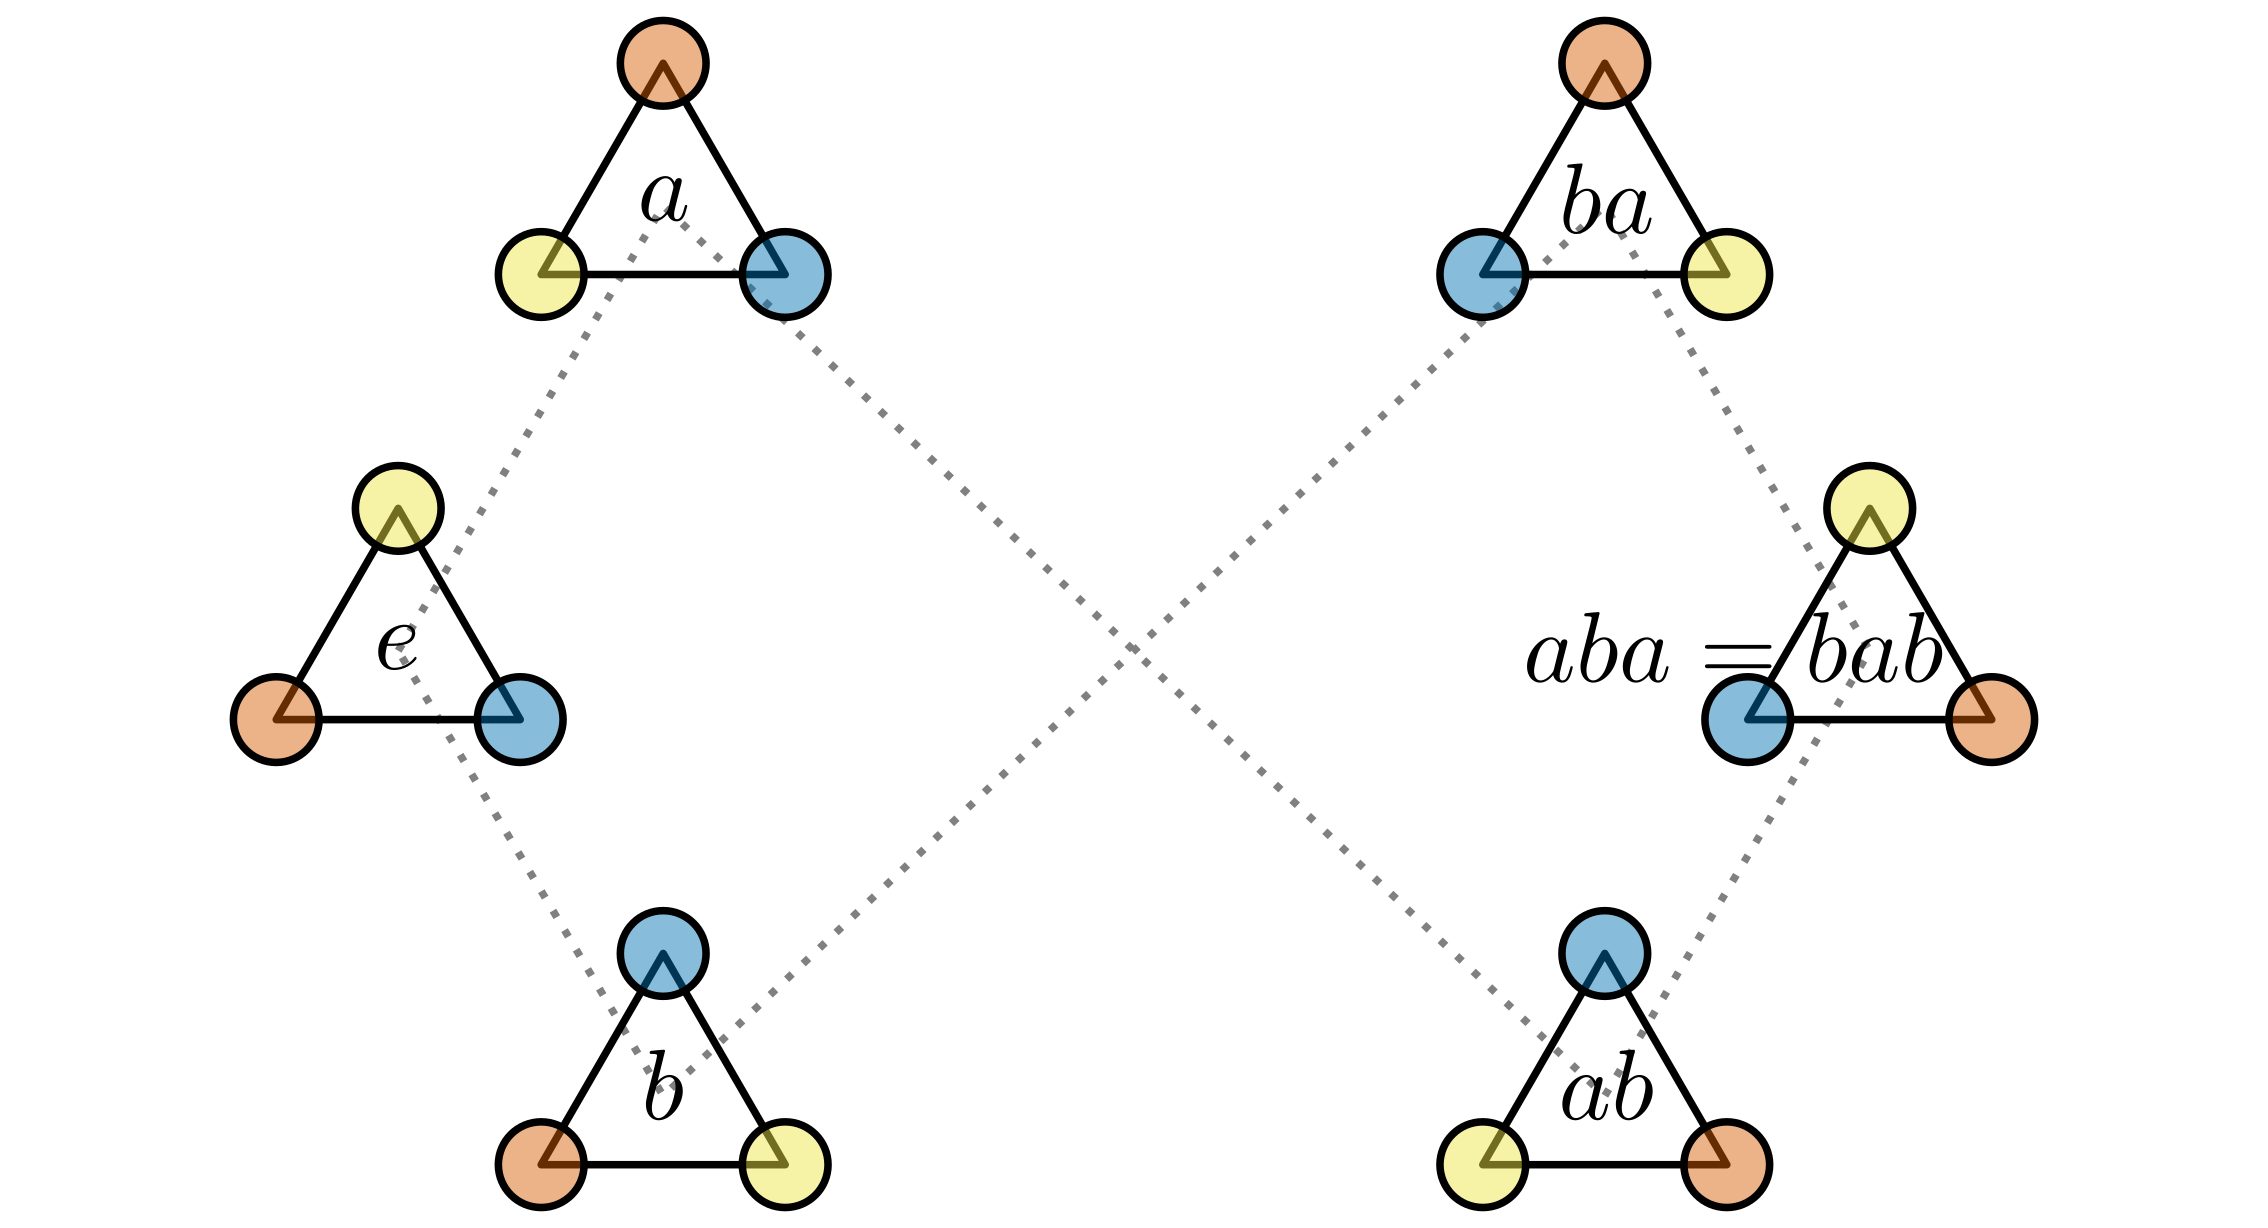
\includegraphics[width=\textwidth]{Figure 13.5.A}
\caption{The group $D_3$ is similar to the flips of a triangle}
\end{figure} \noindent
% Dihedral group of order 3 example
In the above example $D_3$ (the dihedral group of order $3$), the process $\pi_3: baa $ is a length 3 process which may be reduced to $\pi_3: baa = b$. The net result of a process of elementary actions $\{e, a, b\}$ is always an element of this group.

We shall call $\Pi_\ell$ the set of length $\ell$ processes and $\pi_\ell$ to refer to a specific length $\ell$ process, and $\ell$ refers to the number of elementary actions used $\ell \in \mathbb N$. We shall not allow partial or fractional processes $\pi$ in the same way we do not allow partial information units $x$. Both the number of information units $N$ and the length of a process $\ell$ must be finite, and we restrict our definitions of $X$ and $\Pi_\ell$ to be finite compositions or else we encounter the Banach-Tarski paradox.

The Banach-Tarski paradox is as follows. The set of rotations about the unit $2$-sphere is given by the rotation matrices:
\[R_x =
\begin{bmatrix}
1 & 0 & 0 \\
0 & cos(\theta) & -sin(\theta) \\
0 & sin(\theta) & cos(\theta)
\end{bmatrix}\]
\[R_y =
\begin{bmatrix}
cos(\theta) & 0 & sin(\theta) \\
0 & 1 & 0 \\
-sin(\theta) & 0 & cos(\theta)
\end{bmatrix}\] 
\[R_z =
\begin{bmatrix}
cos(\theta) & -sin(\theta) & 0 \\
sin(\theta) & cos(\theta) & 0 \\
0 & 0 & 1
\end{bmatrix}\]
The composition of these actions $\{R_x(\theta), R_y(\theta), R_z(\theta)\}$ for which $\theta \in [0, 2 \pi)$ generates all possible rotations of the unit $2$-sphere:
\begin{figure}[H]
\centering
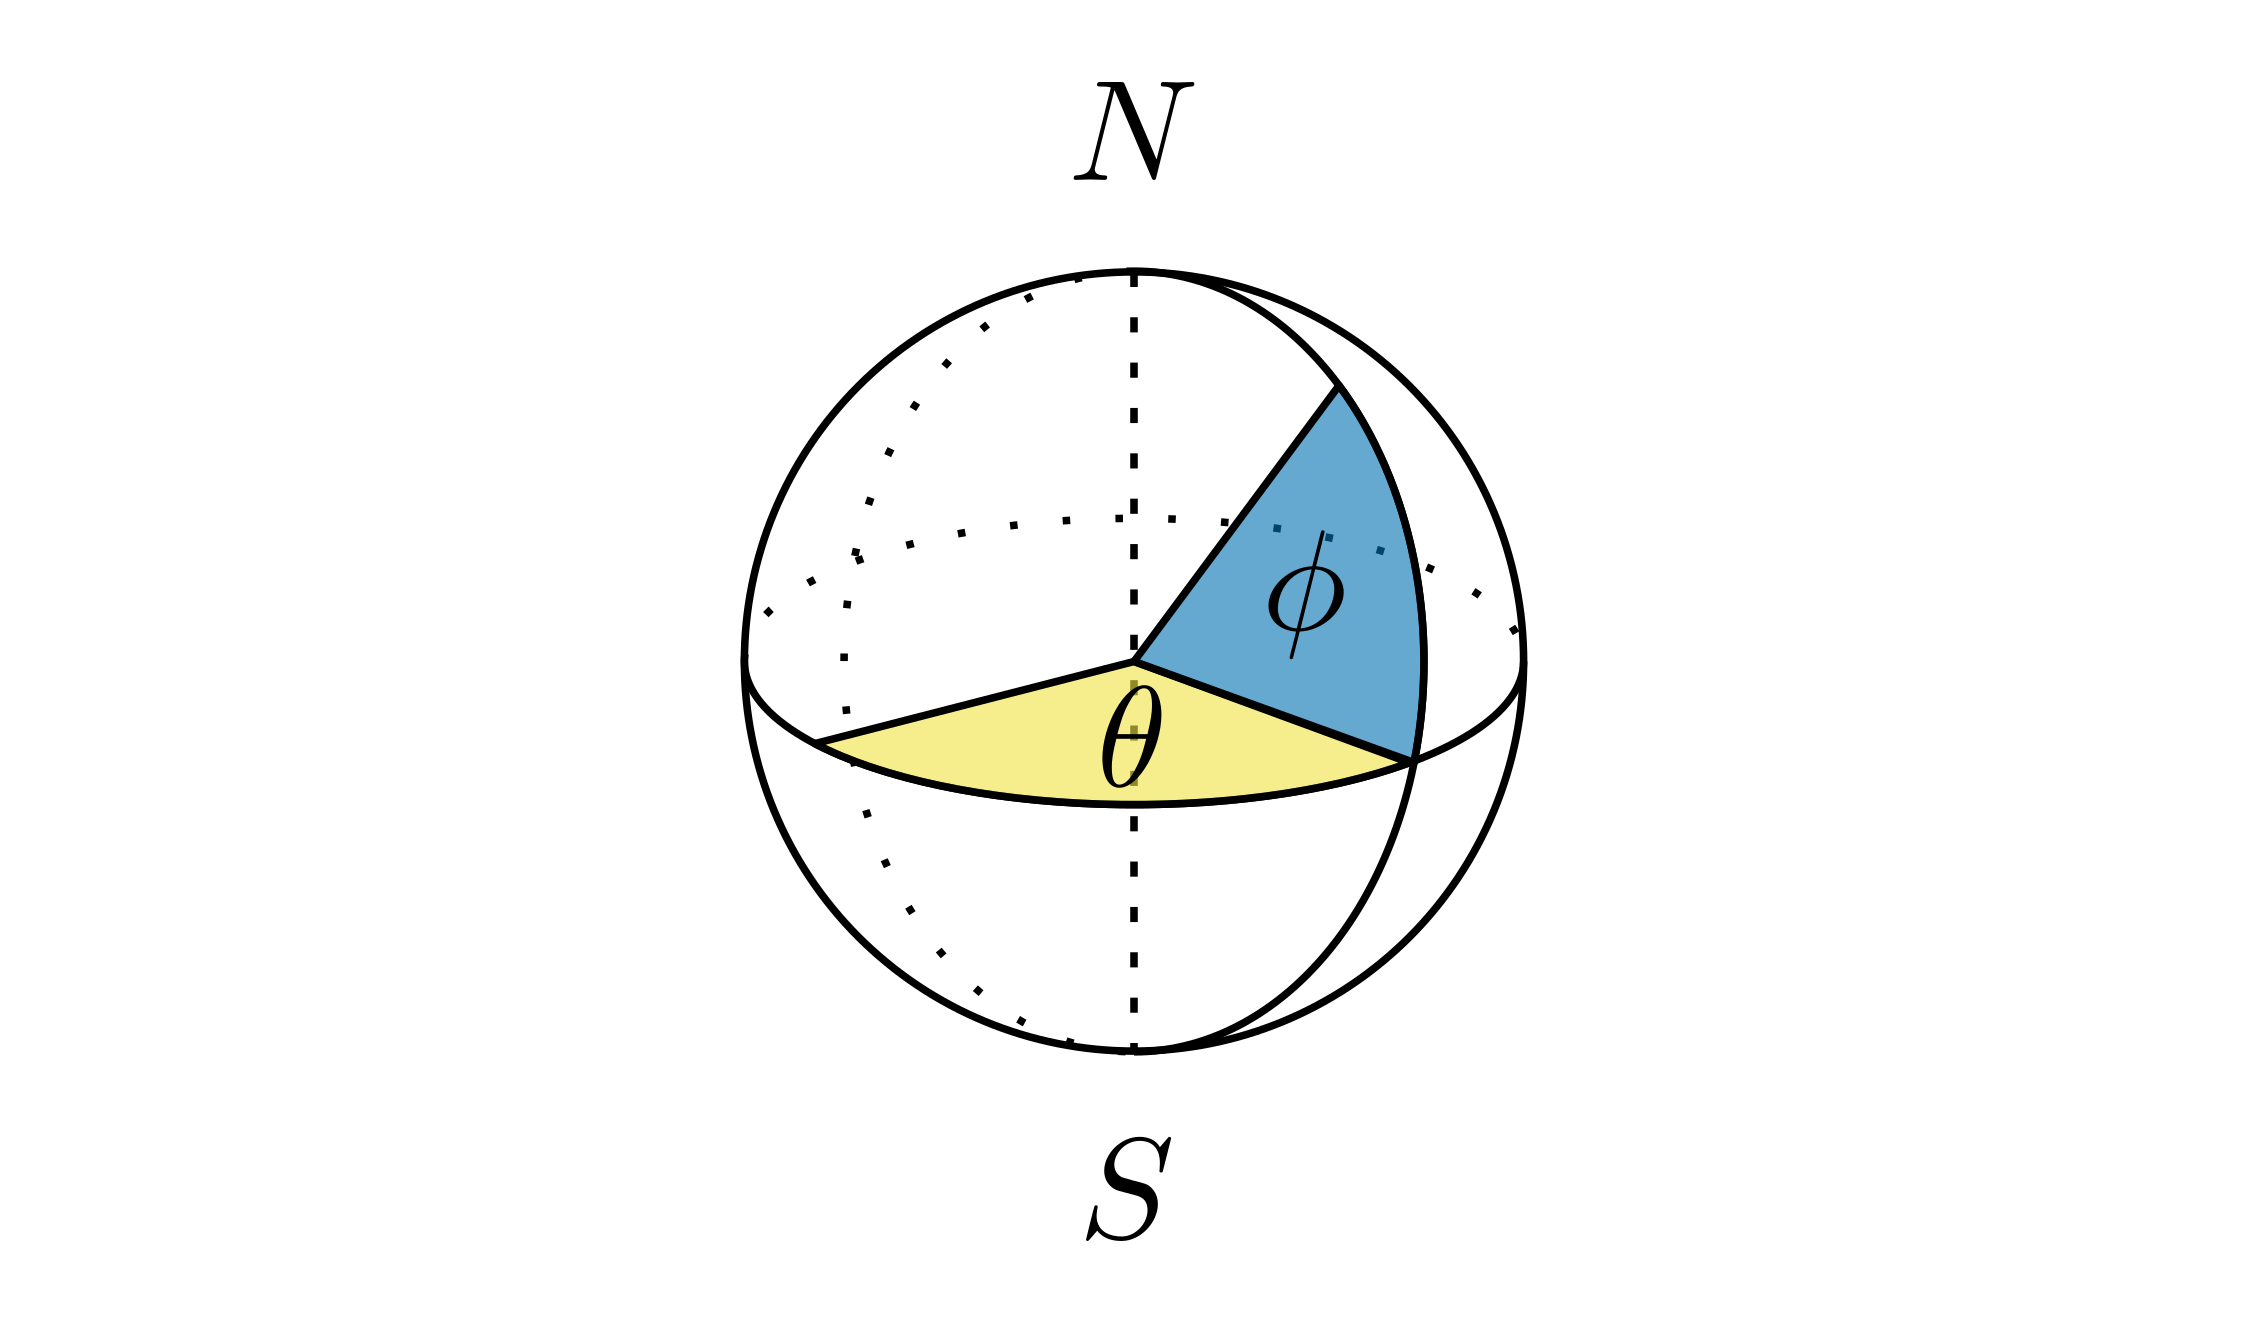
\includegraphics[width=\textwidth]{Figure 13.5.B}
\caption{All possible 3D coordinates on a $2$-sphere can be represented with the horizontal angle $\theta$ and azimuthal angle $\phi$}
\end{figure} \noindent
\noindent % The quaternion actions on the unit 2 sphere.
These elementary actions can generate all possible information states upon the information unit $x$. Using only the actions:
$$\{R_x(1), R_y(1), R_z(1), R_x(-1), R_y(-1), R_z(-1)\}$$ 
upon the Cartesian point $(1, 0, 0)$, the set of countably finite rotations upon this point generates all points of the $2$-sphere $S^2$ such that our information unit is defined as $x = S^2$. Since the ratio between a diameter and circumference is irrational, rotating by the radius will never land on the same point twice. Note that forwards and backwards rotations have a net zero rotation.

Suppose that we separate $x$ into two disjoint subsets $U$ and $D$. The set $U$ is the set of points whose existence begins with the action $R_y(1)$, representing rotating the origin point ``up'' first. The set $D$ is the set of points whose existence begins with the action $R_y(-1)$, representing rotating the origin point ``down'' first. Since the sets $U$ and $D$ are disjoint, their intersection has zero cardinality:
$$U \cap D = \varnothing \implies |U \cap D| = 0$$
We can then perform a length $1$ process $\pi_1 = R_y(-1)$ and $\tilde \pi_1 = R_y(1)$ onto subsets $U$ and $D$ to obtain the following result:
$$U \pi_1 = D \tilde \pi_1 = x$$
Separating the set $S^2$ into two disjoint subsets and applying all possible length $1$ processes generates two copies of the original set, each with the same ``volume''. 

Remember $U \subset x$ and $D \subset x$, and we are saying that $U \pi_1 = x$ and $D \tilde \pi_1 = x$. Since the \textit{rotations do not change the volume} of the set, combining the volumes of these subsets is twice the cardinality of the original set:
$$|U| + |D| = 2|x|$$
Two non-intersecting subsets should have a total cardinality that is less than or equal to the cardinality of the original set $x$, but this may not be true when we are dealing with countably infinite sets. Therefore, we we must consider only countably finite actions to avoid dealing with the Banach-Tarski paradox.

This paradox of volume does not occur in probability because the probability distribution of all actions would normalize to probability $1$. It does however imply that a Wiener process is differentiable nowhere because of it may be infinitely decomposed into infinitesimal paths.

The question is this: How does one decide upon the natural process for continuous information units? If $x$ is a continuous information units such that $|x| = \aleph_1$, then it has the same cardinality $|X| = |x^N| = \aleph_1$ if $N$ is finite. If $x$ is a countably infinite Hilbert space such that $|x| = \aleph_0$, then $|X| = \aleph_0$. What set of processes $\Pi$ would differentiate the computational power of $x$ from $X$?

Let us construct a universe with discrete space in $\mathbb Z^3$ with continuous information units. We allow for continuous time evolution of these units. Suppose that we have information unit $u$ that begins in one of two definite states:
\[|0 \rangle = 
\begin{bmatrix}
1 \\
0
\end{bmatrix}
, |1 \rangle = 
\begin{bmatrix}
0 \\
1
\end{bmatrix}
\]
The pure state $| 0 \rangle$ represents evaluating to $0$ with probability $1$ and the pure state $| 1 \rangle$ represents evaluating $1$ with probability $1$. We have our associated actions given by the Pauli matrices which rotate along the $x, y, z$ axes respectively:
\begin{figure}[H]
\centering
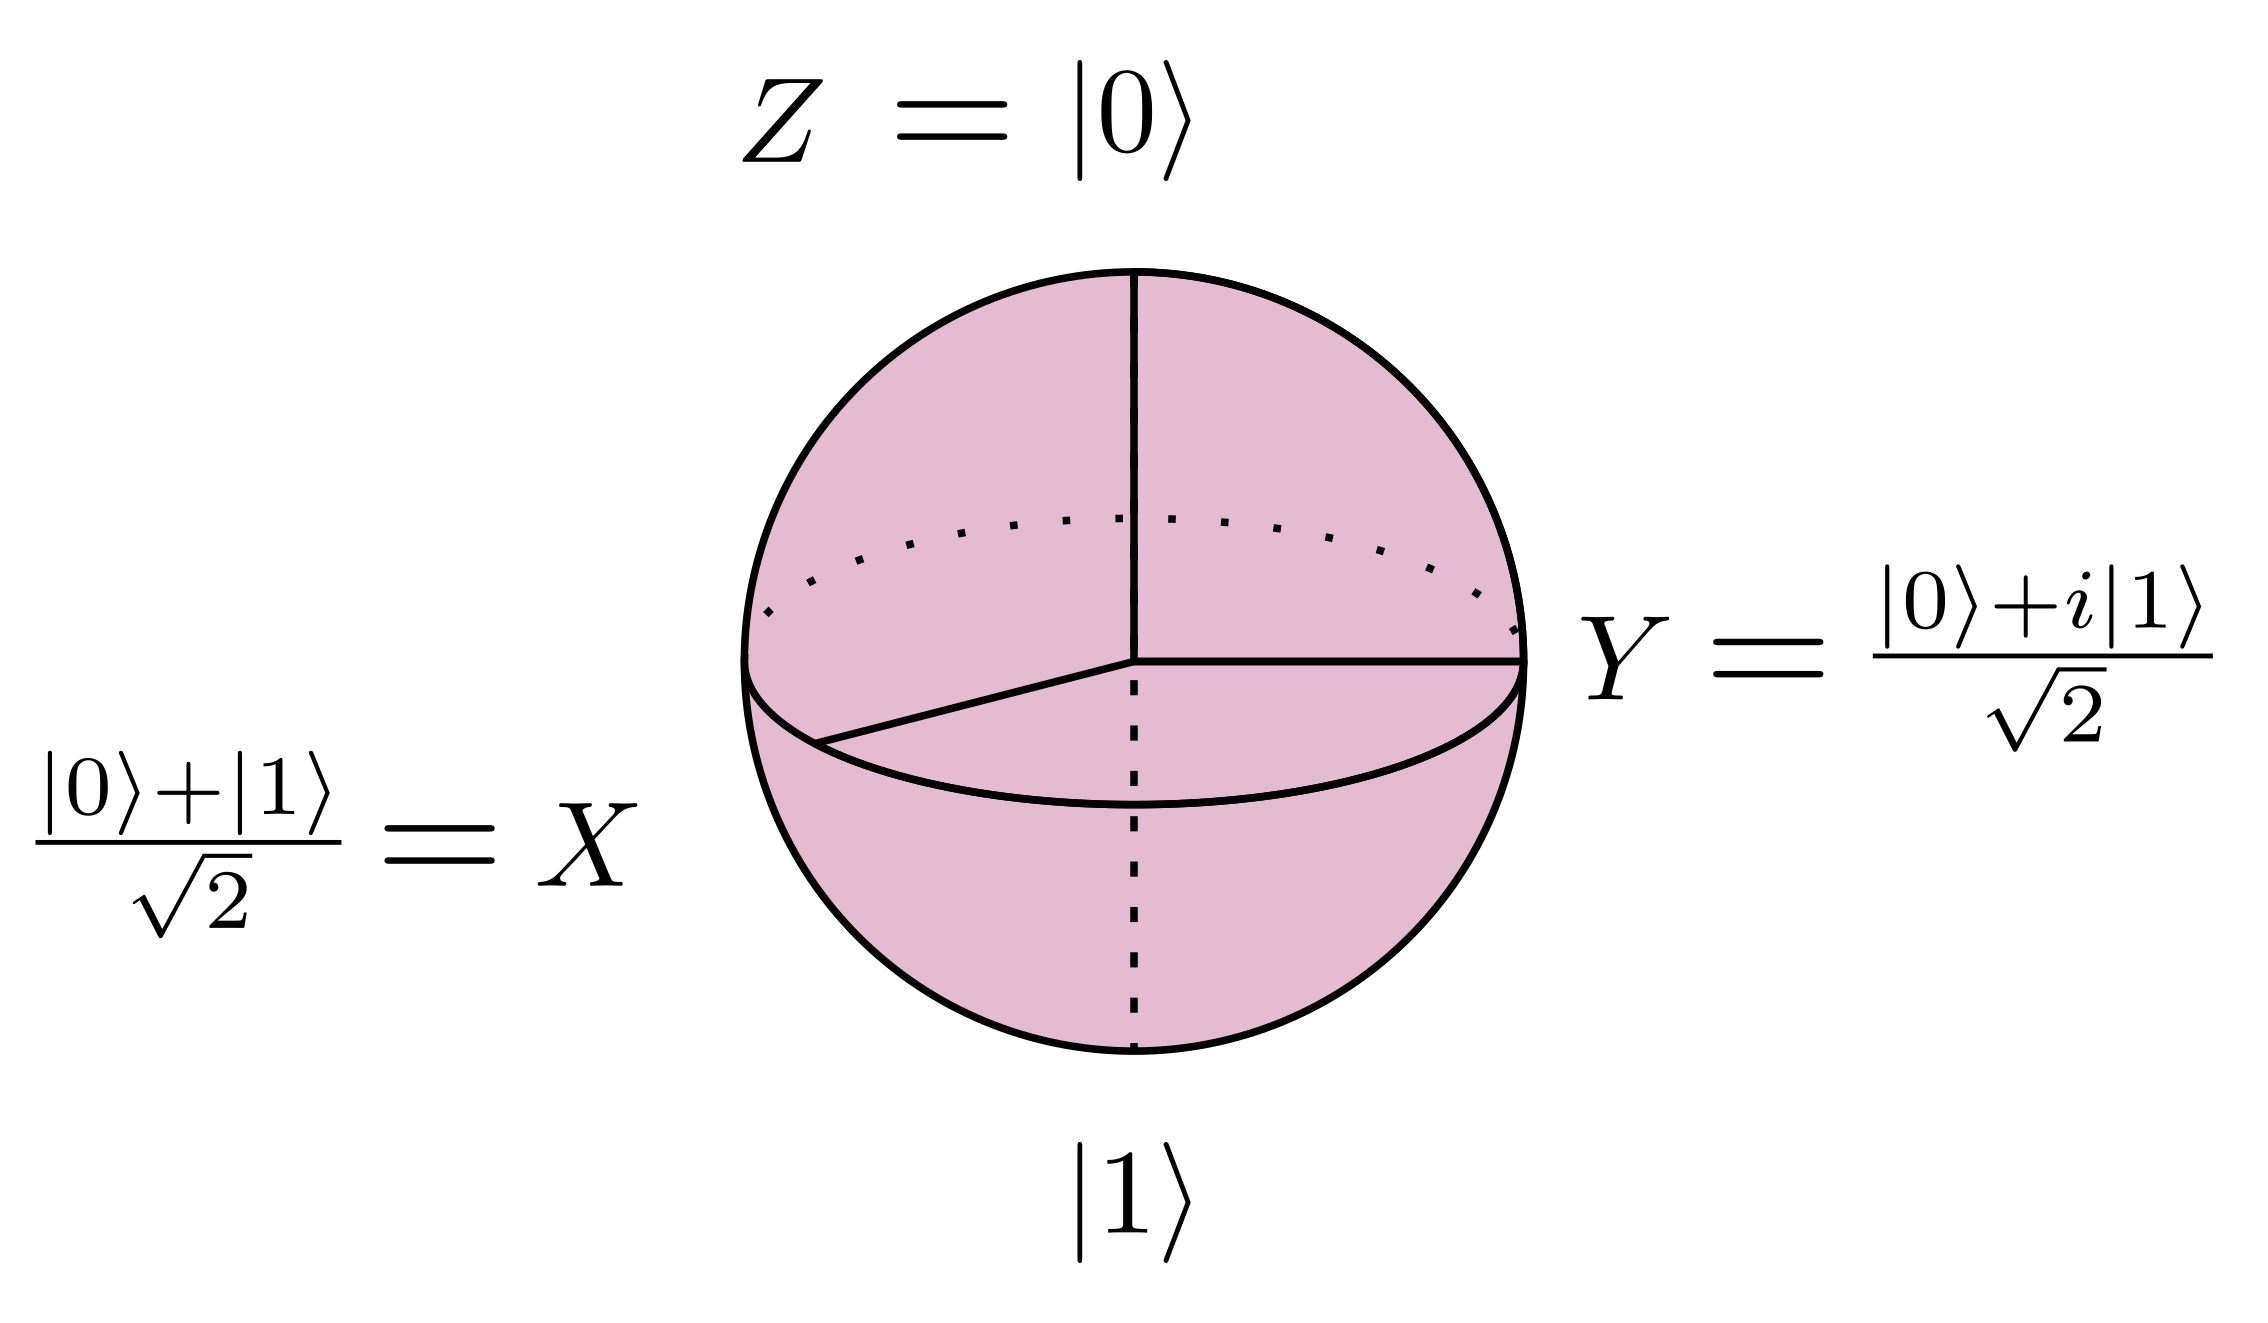
\includegraphics[width=\textwidth]{Figure 13.5.C}
\caption{The Bloch sphere and its axes. We need one less degree of freedom since we assume magnitude $1$.}
\end{figure} \noindent
% The Bloch sphere and its axes
\[
\sigma_x = 
\begin{bmatrix}
0 & 1 \\
1 & 0
\end{bmatrix}
, \ \sigma_y = 
\begin{bmatrix}
0 & -i \\
i & 0
\end{bmatrix}
, \ \sigma_z = 
\begin{bmatrix}
1 & 0 \\
0 & -1
\end{bmatrix}
\]
Now let us supposed we have $N$ information units that compose the information state $U$. What dynamical system allows us to resolve the information units into a definite state? What is the algorithm of conditional probability?

If you were to evolve a continuous information system this way, it would behave as if its value could collapse into one of $2^N$ possible Boolean information states. It does not make sense for a fundamental theory of physics to have ill-defined sequences of conditional probability. If we allow for continuous space, then we cannot allow for infinite curvature of that value over space and time. There would be a fundamental limit, represented by the Planck length and Planck time. 

This is where most attempts to rectify inconsistencies in quantum field theory (QFT) fail: by allowing for Fourier series of increasing frequency as opposed to increasing wavelength. Shannon's limit for channel capacity does not exist in such a theory. The infinities in QFT arise from performing summations over infinitely increasing frequencies. The \textit{action} of a photon splitting into an electron-positron pair and recombining over infinitesimal wavelengths must account for infinite energy.

This is the analytical power of Boolean statistical mechanics and constructivist mathematics. The restriction that our assumptions are minimal allows us to construct understanding of how the universe works with both intuition and rigor, and we can diagnose the problems inherent to current models of any theory.

What are those minimal requirements that we apply to ZFC$\times$?
\begin{enumerate}
\item Binary: An information unit $x$ with cardinality $2$ can approximate any other measure with enough binary units, or bits.
\item Logic: Local interactions of information units may form logic gates given a certain input measure of bits, and their future result is an output computation.
\item Entropy: Any binary set information system state of size $N$ has a entropy rate that is between $[0, N]$ in which $N$ represents statistically independent Bernoulli distributions and $0$ represents a deterministic system. 
\end{enumerate}
The first and second requirements are straightforward enough to explain, but the third requirement is perhaps introduces new concepts. An entropy rate of $N$ means each information unit is statistically independent from the previous state and an entropy of $0$ means each information unit is statistically dependent upon the previous state. An information unit has variable Shannon capacity depending on its neighbors.

\section{The Minimum Requirement of Binary in Patterns}
A \textbf{binary set}\index{binary set} is any set $\mathbb B$ with cardinality $| \mathbb B| = 2$, and it is the minimum measure that may be applied to an information unit $x$ using a probability measure $f$ that creates distinguishable and unique information states called \textit{patterns}. Suppose that we define $\mathbb B = \{\alpha, \omega \}$ in which $\alpha$ and $\omega$ are placeholders for any binary symbols we may prefer. Let $X = \{x_1 ,..., x_N\}$ be an information state with each $x$ being an information unit, or bit if specifically a binary information unit. 

Let $\Sigma$ be the product $\sigma$-algebra for the information units $(x_1,...,x_N)$ and let $E$ be an element of $\Sigma$. Let $g$ be an probability measure, and we wish for $f(E) \neq g(E)$. A prime example would be a physical system whose probabilities evolve with time. This can only occur for if for each $x$ has a cardinality of $x$ is greater than or equal to 2:
$$|x| \geq 2$$
If the cardinality of $x$ is $0$ or $1$, then there exists no unique probability measures such that $f \neq g$. See \textit{Figure 12.1} for a visualization.

If we let $\alpha = \omega$, then it is always true that $f(E) = g(E)$ since we have the isomorphism: 
$$\{\alpha, \alpha \} \cong \{ \alpha \}$$
due to duplicate elements in a set being compressed. The product $\sigma$-algebra is $E = \varepsilon_1 \times ...\times \varepsilon_N$, and it has one valid state to measure which is given by:
$$f(\alpha_1 \times ... \times \alpha_N) = g(\alpha_1 \times ... \times \alpha_N) = 1$$
for all $N \in \mathbb N$ natural numbers and for all probability measures $f$ and $g$. Since we define sets to no duplicate elements such that $\{\alpha, \alpha\} = \{ \alpha \}$, there is only one valid probability measure such that $f = g$. Furthermore, this probability measure is entropy $0$.

If there exists a sub $\sigma$-algebra for the information unit $x$ that may represent a time-evolving system, then $x$ is not minimal. Suppose that we create a $\sigma$-algebra by removing some elements of $x$ then merging them with the leftovers of $x$. There are many ways to select elements to merge with others. We call these the \textbf{sub $\boldsymbol \sigma$-algebras}\index{sub sigma algebra}, and specifically:
$$\tilde \varepsilon = 2^{|x| - k}$$ 
is the cardinality of the subalgebra when we perform $k$ merges on a single information unit $x$. If the number of subalgebras that we may define is less than or equal to $1$, then it is not possible to \textit{minimize} the information unit. 

A simple example to compare is quaternary, ternary, and binary. We can perform a $1$-merge of the quaternary elements $\{ \alpha, \beta, \gamma, \delta \}$ in ${4 \choose 2}$ different ways, and we get a ternary set with the elements $\{ \alpha_1, \beta_1, \gamma_1 \}$. We can perform a second $1$-merge in ${3 \choose 2}$ different ways, and we get a binary set with the elements $\{ \alpha_2, \beta_2\}$. We can perform a third $1$-merge in ${2 \choose 2}$ way, and we get a unary set with the elements $\{ \alpha_3\}$. Regardless of \textit{how} we merge elements, the size of the sub $\sigma$-algebra always decreases by a factor of $2$ because merging is a binary operation. Any $k$-merge is inherently a sequence of $k$ binary operations, and its inverse operation would be called a $k$-split.

The number of unique possible product $\sigma$-algebras composed of $N$ copes of the information unit $x$ after a $1$-merge is given by:
$$2^{N(|x| - 1)} = 2^{N|x| - N}$$
It is not possible to deconstruct to a sub $\sigma$-algebra if $|x| = 0$ or $|x| = 1$. There is the strange case where the number of unit subalgebras of $x = \varnothing$ is given by:
$$2^{(|x| - 1)} = 2^{0 - 1} = 2^{-1} = \frac{1}{2}$$
but we are assuming that this is irrelevant for most cases of interest. The number of unit subalgebras for when $|x| = 1$ and $k=1$is given by:
$$2^{(|x| - 1)} = 2^{1 - 1} = 2^{-0} = 1$$
Since the case of $|x| = 2$ cannot be minimized to a smaller information unit and still represent a time-evolving system, the Boolean set $\mathbb B$ should be of the utmost interest to all dynamical systems theorists. 

If you were to argue that the base information unit of x should have a cardinality of $3$, remember than $|\mathbb B|^2 = 4$ means that the Boolean set can represent all possible information states of information units greater than cardinality $2$. We may alternatively perform a $1$-split of a binary set to get a set of ternary set, and this brings us back to the recursive problem that merging is a binary operation and splitting is an inverse binary operation.

An assumption about our current universe that we take for granted is the distinguishability between objects. Obviously, non-distinguishability means that a universe with evolving patterns cannot exist. It is not that a ternary universe is impossible per se, just that the binary system is more ``natural'' as it is more minimal. Although not a rigorous argument, the fact that the power set of $A$ is given by $2^A$ implies a sort of informal naturalness about base $2$ and compositions of sets of cardinality $2$. It also helps to remember that $\log_b (x)$ with base $b = 2$ is the smallest valid base from the set of natural numbers $\mathbb N$.

\section{The Minimum Requirement of Logic in Computation}
A \textbf{logic gate}\index{logic gate} is a realization of an ideal logical function, and its mapping of Boolean information states $f: \mathbb B^m \rightarrow \mathbb B^n$ via probabilities is the minimal logic that creates objects that are necessarily computable. Any physical model of reality that may be finitely approximated on a computer via simulation is necessarily a computable model. This is important is we are considering what the point and purpose of scientific fields of study are in the first place and why they require data. A photon obeying the mathematical laws of physics may not fail to exist as a specific pattern on a computer. In fact, photon is a word in the lexicon precisely because \textit{language is a model of computation} in which words or lexemes often refer to a specific object or operator (nouns and verbs)

This is a metaphysical argument, but for physics to be capable of constructing finite \textbf{Turing machines}\index{Turing machine} via abstract diagrams, the laws of physics must be \textbf{Turing complete}\index{Turing complete}. Likewise, for a human mind to have conceived the idea of a Turing machine as Alan Turing once did, the human mind writing in natural language must have embedded within laws of linguistics that are Turing complete. If you have a device whose rules may map $f: \mathbb B^m \rightarrow \mathbb B^1$ for $m \in \mathbb N$ and it may extend via composition to have $f_1 , ... , f_N: \mathbb B^M \rightarrow \mathbb B^N$ for any $M, N \in \mathbb N$, then those rules are Turing complete and the device is a finite Turing machine.

It is easily forgettable that physics, linguistics, and mathematics must operate on a Turing complete basis of rules. It is necessary that Boolean information states and maps between them via Boolean algebra are minimal representations that may construct their higher-order representations. Boolean algebra is a form of \textit{zeroth-order logic} while physics, linguistics, and mathematics are forms of \textit{first-order logic} whose logical connectives lack definite true or false answers. In other words, mathematics, physics, and linguistics seeks relations between indefinite structures using defined relations. The linguistic question ``Will it rain tomorrow?'' has a dependency on the undefined variables ``today'' and ``today's weather data'' as well as the more esoteric ``conditions on the surface of the sun''. The gradient operator $\nabla$ acting on a function $f$ indefinitely defines $\nabla f$ via \textit{static typing}.

Mathematics is statically-typed and linguistics is dynamically-typed. By type, we mean the following:
\begin{enumerate}
\item Statically-typed: The variable's \textit{type} or structure is defined upon creation.
\item Dynamically-typed: The variable's \textit{type} or structure is inferred upon evaluation.
\end{enumerate}
We might say then that physics is a hybrid of these two approaches. The linguistic variables ``black hole'' and ``theory of everything'' are dynamically-typed because they are undefined for the conjectured parts but they are statically-typed for the understood parts.

\section{The Minimum Requirement of Entropy in Information}

Entropy is simultaneously the \textit{complexity of a system} and the \textit{information capacity of a system}. Therefore a system with an entropy of $N$ can only be simulated by a system with an entropy of $N$ or greater. Entropy is the representational power of a system: a larger system cannot be completely accounted for by a smaller entropy system. This does not mean that a physical system of larger volume cannot be represented for by a physical system of smaller spatial volume. The computations of a large room with few baseballs can be represented by small human brain. This is because the degrees of freedom of what we conceive as ``baseballs'' is dramatically smaller than the degrees of freedom in the neural state space.

As a reminder, the formal definition of entropy of a continuous probability distribution $f$ is given by:
$$S(X) = - \int\limits_{x \in X} \ln (f(x)) f(x) dx $$
The continuous entropy (or differential entropy) is the default definition of entropy. Alternatively, the definition of Shannon entropy of a discrete probability distribution is given by:
$$S(X) = - \sum\limits_{x \in X} \log_2 (f(x)) f(x) $$
The Shannon entropy roughly captures how many binary information units one would need to completely represent all possible states of the discrete probability distribution.

We claim that any binary set information system state of size $N$ has a entropy rate that is between $[0, N]$ in which $N$ represents statistically independent Bernoulli distributions and $0$ represents a deterministic system. When we are considering computational information systems in general, we need to consider that the maximum entropy rate of the system should scale with the size of the system. This does not means that the computational information system is necessarily maximizing its entropy rate at any given time: rather its expected entropy rate tends to average out depending on the probability of each specific state at some point in time.

We may define non-zero entropy for a probability distribution if the cardinality of an information unit $x$ is greater than or equal to $2$. Entropy in a computer science sense is relatively simple: More binary information units (bits) means more computational power. It is impossible for a smaller amount of bits to represent a larger amount of bits without information loss. Entropy in the probability sense means that a fixed coin is equivalent to needing only $N-1$ coins to represent the number of possible states of all $N$ coins. It also means that N coins that are not perfectly fair can be represented by less than N coins. The sensibilities of binary systems is something that we may have a strong intuition of by now. Measuring entropy becomes infinitely trickier if we allow infinite cardinals such as $|x| = \aleph_0$ or $|x| = \aleph_1$.

This brings us to the issue of when we have an information unit whose cardinality is an \textbf{aleph number}\index{aleph number} such as $\aleph_0$ or $\aleph_1$. What is the number of subalgebras of an information unit after $k$ merges, assuming that the cardinality of $x$ is an aleph zero? What about aleph one? We cannot reduce a continuous space by using a countably finite number of merges. This again raises the issue of the continuum hypothesis which is true under our chosen axioms of Zermelo-Fraenkel Constructibility.

Under the ZFC$\times$ axioms, it is possible to \textit{minimize} the continuous information unit of $|x| = \aleph_1$ if we perform $\aleph_0$ merges. Without \textbf{axiom of constructibility}\index{axiom of constructibility}, we cannot assume that a continuous information unit can be represented using discrete information units. If the universe operates on the principle of continuous information units, then what transition function preserves the volume but changes the entropy in a way that is scale invariant? If we consider continuous information units upon discrete time and discrete space, then any appropriate transition function is not scale invariant. 

If we consider discrete time and continuous space, then we encounter the Banach-Tarski paradox in assigning a probability to the process distribution. This is due to the reversibility of a Wiener-like process: As we move along space, we need to define an action along each point in space to define a spatial process. The recursive self-similarity would create infinite entropy. If we split our spatial process into intervals of being net increasing or decreasing, and we can assign a Boolean set to each interval. Since two intervals of arbitrary length are self-similar, they have the same information capacity regardless of length. Suppose we assign a probability using a sigmoid function $s$, and we use a sigmoid function upon the finite difference between two points of a Wiener process $s(\Delta x)$. This assignment still creates the self-similar information capacity problem. To avoid infinite signal energy and information capacity along a spatial path, there must be a maximum frequency.

What makes two continuous information units have more computational power than one continuous information unit? The number of possible states of N continuous information unit is given by:
$$\prod\limits_{i=1}^N |x| = |x|^N = \aleph_1^N = \aleph_1$$
The entropy of each information unit is limited by whether we define $x$ to be something like $x = [0,1]$, $x = [0, \infty)$, or $x = (-\infty, \infty)$. However, there is no specific rule that prevents the entropy of a single information unit from representing the dynamics of multiple information units. Its internal information state may be a universe unto itself \textit{unless} the dynamics have sufficient smoothness and finite energy. Referring back to the Bloch sphere in \textit{Figure 12.6}, a known state from $| 0 \rangle$ must decay to the uniform state relative to any two basis vectors and not some infinitely jagged mess. Any dynamical system describing the diffusion of a known point upon the Bloch sphere must fulfill the Lebesgue integrability condition. Otherwise, the (unconditional) probability is not computable.

We wish in some sense that the dynamics of $N$ information units cannot be represented by a system with less $N-1$ information units. There is a cognitive bias for discrete systems if you consider that I am using the word ``unit'' while simultaneously typing using the Modern English alphabet, a discrete information system. The letters make words, words make sentences, sentences make paragraphs, paragraphs make sections, sections make chapters, chapters make parts, and parts make this book.

When we discuss the nature of entropy in a computational information system, I mean is this: \textit{What is the natural course of the increase in entropy of an information system? Why should it change at all, and why is the way it changes non-deterministic?} These questions fall short of any rational or empirical explanation, but perhaps they lie in the domain of constructivist explanation. 

My fundamental hypothesis is that the universe will execute every computable function, and the only way to do that is if the probability of each function is non-zero given an infinite amount of time. Considering that we anticipate the universe to be infinite in space as well, that means it already is executing every computable function, already has executed every computable function, and already will execute every computable function. The second Borel-Cantelli lemma makes arrivals forward in time and anywhere in space obvious, but backwards in time is complicated considering the inverse of a stochastic matrix is not a stochastic matrix. We rely on the fact temporal transitions on the infinite lattice $\mathbb Z^d$ are spatial translations of the same infinite state, the paradox of the infinite repeating pattern discussed in \textit{\S 9.2 Notation and Convention}.

I quote my young high school self once again. ``A probability is a possibility. A possibility is an eventuality.'' In such a system, one will eventually be proven wrong that something is impossible so long as it is computable. This is not to say that such a computable universe is inorganic, hostile, robotic, and static. It is wild, beautiful, romantic, and artistic. Abandon certainty, for this universe does not operate on such a principle.

\section{Degeneracy to Wuji if Requirements Not Met}
In Daoist philosophy, \textbf{wuji} (無極), defines things that are without limit, infinite, or non-polar. This is in contrast to the concept of \textbf{taiji} (太極) which defines things that are limited, binary, and polar. The taiji is composed of \textit{yin}, or dark, and \textit{yang}, or light. What purpose does existentialist philosophy have in a mathematics textbook?

Without polarity, things would not exist. Without logic, the universe would be pure chaos. Without entropy, the universe would be lifeless order. All of these components are necessary to make a universe with no beginning or end, a universe with endless possibilities, a universe that may be understood by itself, and a universe that will tell every story.

Consider the consequences of non-polar systems. There is no attraction and repulsion between objects. There is no flow between objects. Existence is defined by boundaries. If the flow between objects may be reduced to truly neutral without the chance of becoming polar again, all existence in the universe will cease to exist. The heat death of the universe is one such example of non-polarity.

Consider the consequences of non-logical systems. There is no specific sequence that may be predicted or inferred. The objects that exist represent nothing in particular, realizations that point toward no idealization. A limitless system can also compute everything that may exist immediately without restriction. Patterns would be meaningless because they are all equally probable at any point in time and space.

Consider the consequences of non-entropic systems. There is no way for any object or person to escaped its defined fate. The stories say or songs that we sing have a defined order. The universe is no longer mysterious and full of wonder is it becomes more and more known. All comes towards an inevitable conclusion, and there is no chance to recover. Only Laplace's demon, the lone $\sigma \tau o \chi \alpha \sigma \acute \eta \varsigma$ (stochast\'is: thinker) in this universe, would be able to gaze upon the infinite past and infinite future to change the flow of fate.

What would such an empty universe look like? A universe that defines non-existence cannot exist in the sense that it is a computational impossibility. This is not to say that non-polar universes may not exist somewhere. This is not to say that non-logical universes may not be considered in the formal languages of the mind. This is not to say that non-entropic universes may not be represented as a toy representation of the mind. But these universes do not appear to be ours. That I can say with unity, with faith, with certainty.

\section{Linguistics of an Object}
An object as described by a \textbf{noun} is a set of space whose entropy rate is approximately linear within the boundary, and this entropy rate has a sharp discontinuity at the boundary. The entropy rate also does not change with respect to some permutation of the interior. The entropy of signal types may differ in its interaction with the boundary be they pressure waves of electromagnetic waves, but linearity and discontinuity conditions tend to be preserved upon interaction with these waves or signals. 

Consider a lake of water on planet Earth. Permuting the water in the lake in small patches is unlikely to chance anything dramatically because most permutations of that object maintain its perception as belonging to an eigenclass. For recursive definition, water is water because permutations of water in a small neighborhood are computationally indistinguishable. In most cases, even large patches of water in a large neighborhood may be exchanged yet be computationally indistinguishable. I say \textit{most} cases because a cup of water with ice does not behave similarly with respect to small neighborhood permutations of the liquid water and frozen water, even though we identify water as being composed of water molecules. 

When an object has a sub-object with greater entropy rate, that component gets a name or noun. This is the nesting nature of attention. For example, a cell's nucleus or a human's brain have closed boundaries in which the entropy sharply increases per unit volume. These computation heavy, control center type objects cannot be mixed without significantly distorting what they represent and how they interact with the world. However, most objects are permutable within themselves (water with water) but not with other objects (water with air). The correlation of the future of a calm basin of diluted water and permutations of that water are quite high. While the entropy rate of water is quite high, the entropy rate of critical components using water is even higher.

The rule of attention is that smaller components or objects are named because of their entropy rate density. Power sources, control centers, pivot points, places of cultural significance, and the many wonders of the world. A prime example is how a coral reef is named due to its biological diversity being high; in my terminology, it is named for high entropy rate density. Due to the limited information capacity of any organism, a smaller computing system $A$ can best represent computing system $B$ by modeling the critical components of $B$.

Artificial machines or mechanisms are special because of their sensitivity to permutations of patches of space. Biological machines and mechanisms are likewise fragile, but they have a particular sort of resilience in their ability to heal from damage. A machine or mechanism is component dense with almost every part having a purpose. This means that machines are highly nonlinear with respect to measures of some entropy rate density function:
\begin{figure}[H]
\centering
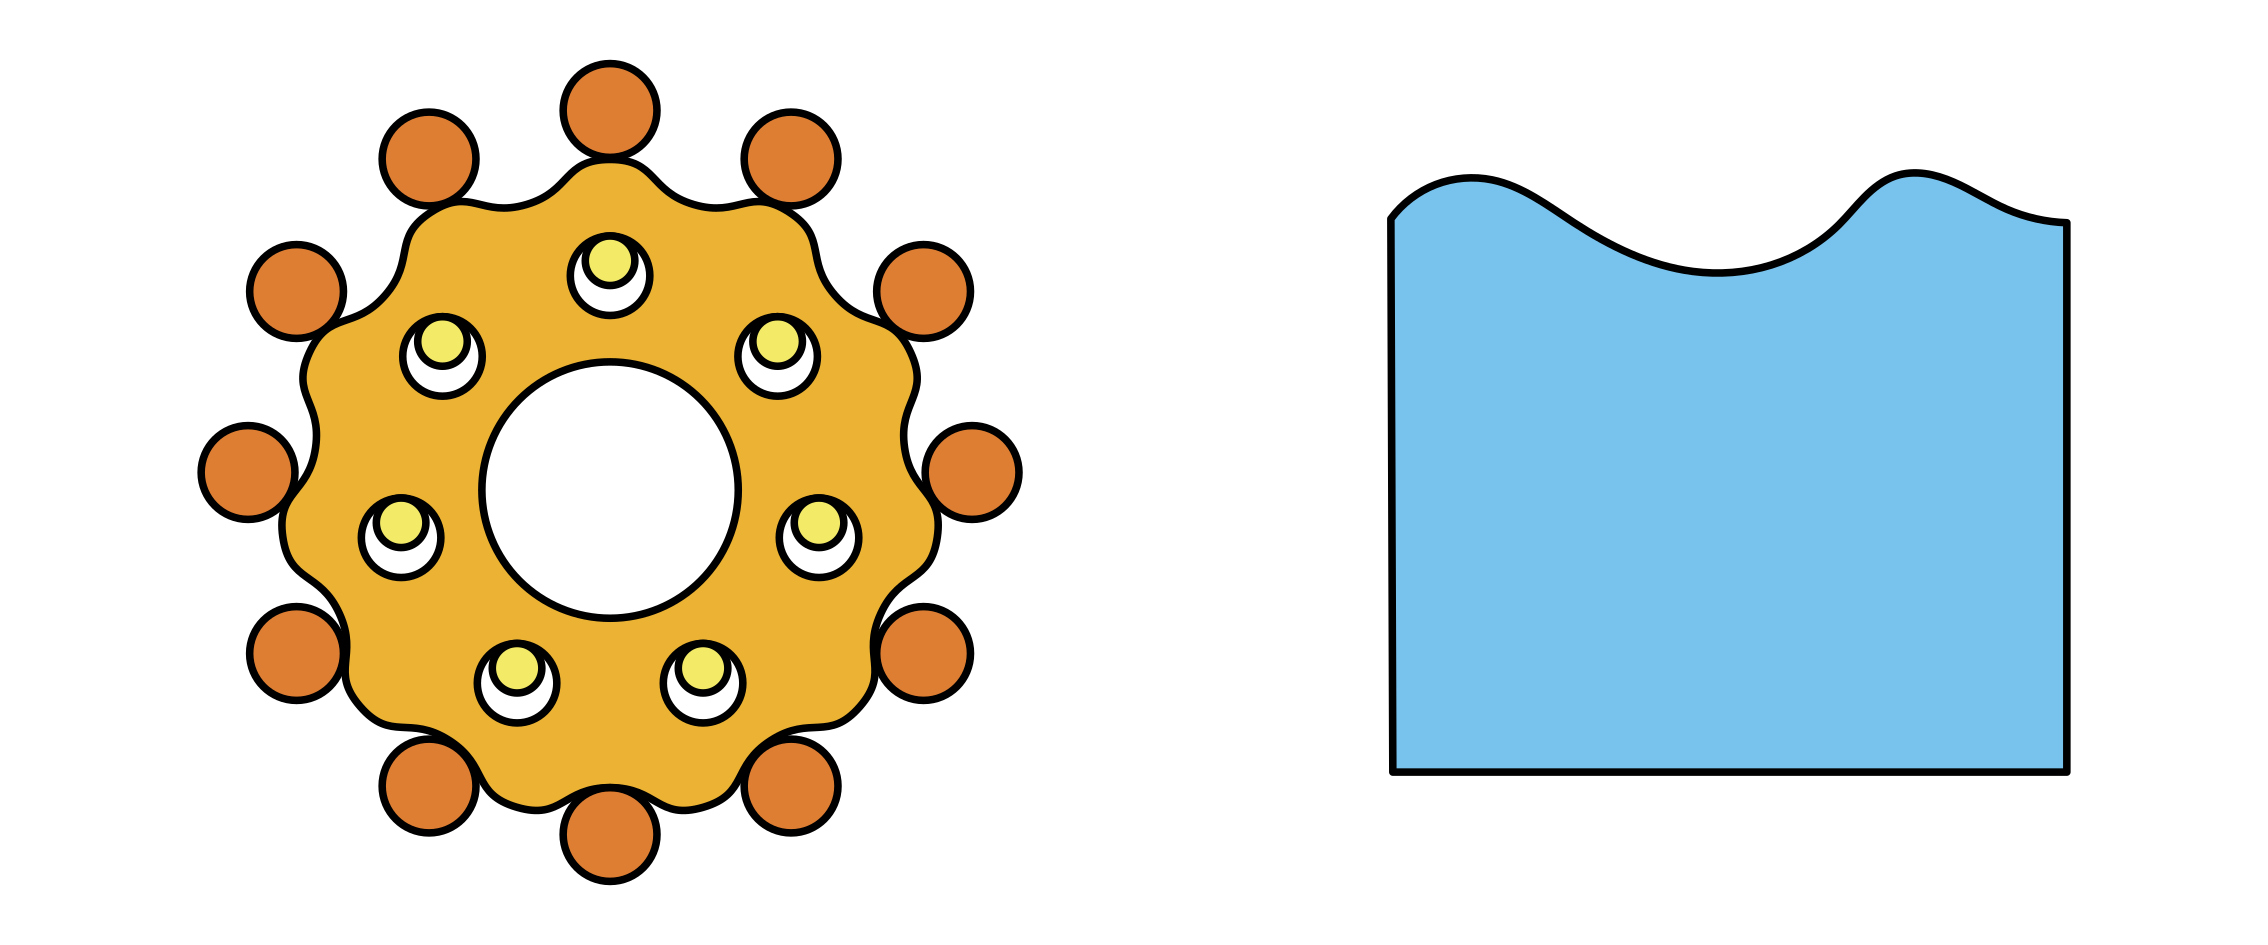
\includegraphics[width=\textwidth]{Figure 13.10.A}
\caption{A cycloidal drive is a sensitive; water is insensitive}
\end{figure} \noindent % Diagram of some artificial mechanism in contrast with a non-mechanism
A cycloidal drive would be thrown off course if it were to be deformed, which is why they are often made of hard materials such as low-carbon steel. A non-mechanism like water is less sensitive to permutations, even though fluids are capable of complex mechanics and computation. We reiterate that water is identical and exchangeable in most cases.

Could we not simply judge object differences by material properties? The answer is no because material properties are derived from measured signals. Any object communicates to other objects via signals, and these includes interior components of a mechanism with each other. Variation or change in the expected signal tells us that our object has changed, we have changed, or our model is wrong.

In order to determine the similarity between objects, we can measure KL-divergence of probability distributions $f$ and $g$:
$$\textnormal{KL}(f, g) = \int\limits_{- \infty}^\infty f(x) \ln \big( \frac{f(x)}{g(x)} \big)$$
which is zero when $f(x) = g(x)$. Kullback-Leilber divergence measures differences in a signal's true distribution $f$ given a substitute or model $g$. We can use any sort of event distribution $f$ be it how an object looks, sounds, feels, tastes, or smells. To a human, objects are immediately identical when they fool all five senses. This is why bad products pay for advertising while vendors purchase authorization to sell good products.

Instead of measuring a signal using KL-divergence, we can alternatively measure the divergence of the resistance that a signal experiences. But remember that most important thing that defines the boundary of an object is that what you predict about its future and how it interacts with its environment differs from other objects. There is no data to collect on how they differ is only discovered with death. Built-in warning signs are far better than durable materials that critically fail without notice.

\chapter{Questions in Current Physics}
At the time of writing this textbook in 2024, physics has been successful in describing the laws of nature. Technology dependent upon its predictions has allowed for great comedy and tragedy to occur in its name, the pride of the 20-th century. Golden ages are tainted by hubris. True science is sidelined in favor of weapons of science. We think ourselves rational, enlightened beings. The reality is that we are human, all too human.

At the time of completing this textbook in 2026, anti-intellectual policy has risen in the United States. Projects like this textbook are only possible with an innocent desire to understand the world. It shall make no man rich in the present. It provides no man advantage over another. It cannot be hoarded, coveted, or stolen. The science of today was built by those who gave knowledge freely in the past. That science may be gone tomorrow.

Some of the questions that we seek to answer are of a pragmatic, worldly interest. Other questions that we seek to answer are of erotic, transcendental interest. I personally do not seek answers so much as good questions. A good question can be savored for days on end, weeks, months, perhaps even years. With the right question, the taste of struggle is just as sweet as success. The questions we seek to ask about physics require more than asking about data, proof, and solutions. The questions require introspection about our fundamental assumptions, interpretations, and self-discovery.

Ask yourself these questions. Will my physics department ever be funded for non-military and non-corporate reasons? It is not that they are bad or unimportant questions, but the ideals of science are often sacrificed in their name. What good is it to spend most of your youth becoming a scientist to waste the rest answering someone else's questions?

I will dare to ask these questions, and I urge you to come along with me. Not as a teacher, student, grantor, or employer. Let us walk through these questions as intellectual equals.

\section{Planck Length, Mass, Time, and Force}
Does the Planck length as corresponding to some universal pixel? Such questions are quickly shut down in online discussion, arguing that our universe is isotropic.\footnote{Random walks are asymptotically isotropic, meaning the infinite past of a Boolean random walk \textit{is} isotropic. This makes detecting anisotropism impossible because the measurement device also has an infinite past that causes isotropism.} Since the dominant philosophy of the natural sciences is empiricism, analytic interpretations using rationalism are devalued. ``Shut up and calculate!'' once said David Mermin. Yet it is plain as day that the Planck length $\ell_P$:
$$\ell_P = \sqrt{\frac{\hbar G}{c^3}} = 1.616 \times 10^{-35} \ \textnormal{meters}$$
demands philosophical inquiry. What does it mean for the gravitational constant $G$ and the speed of light $c$ to define some unit length?

If we leave the derivation of conclusions to empirical measurements alone, the uncertainty principle:
$$\sigma_x \sigma_p \geq \frac{\hbar}{2} = \frac{h}{4 \pi}$$
guarantees that we shall not get an exact answer. The philosophy of empiricism is defeated by computational indistinguishability unless we think more deeply. If our scientific tools become increasingly unreliable as we investigate smaller space and time scales, we need to ask more fundamental questions. Why do measurements become unreliable at small length and time scales? Why are objects become more deterministic at larger scales? How is the scientific method restricted by classification as discussed in \textit{\S Appendix D: Class Stochastic Matrices}? Is it possible to skip the classification scheme of the scientific method, thus deriving the theory of everything from first principles? We must dare to ask these questions.

Other Planck units may be derived from the Planck length $\ell_P$, often requiring the reduced Planck constant $\hbar$. We may obtain the Planck time $t_P$, the Planck mass $m_P$, and the Planck temperature $T_P$.\footnote{I argue the Planck coldness $\beta_P = T_P^{-1}$ is more fundamental to statistical mechanics than Planck temperature.} The reduced Planck constant $\hbar$ is in units of angular momentum of $\textit{mass} \times \textit{length}^2 / \textit{time}$, and energy has units of $\textit{mass} \times \textit{length}^2 / \textit{time}^2$. The reduced Planck constant $\hbar$ may therefore be interpreted as the time integral of energy.

The reduced Planck constant $\hbar$ has a value of:
$$\hbar = \ell_P \cdot m_P \cdot c = 1.05457 \times 10^{-35} \ \ \textnormal{Joules / second} $$
An electron may have a spin of $\pm \frac{1}{2} \hbar$, corresponding to a half-spin of up or down. If we are to say something as incoherent and non-sensical as $\mathbb B = \{ -\frac{1}{\mathbb B}, +\frac{1}{\mathbb B}\}$, then we can derive some other strange interpretations from it as well:
$$\mathbb B = \pm \frac{1}{|\mathbb B|} \iff \mathbb B \cdot |\mathbb B| = \pm 1$$
I would not take this definition recursion of the Boolean set seriously, but the point is to free your mind from undue conceptions.

Note that the Planck energy $E_P$ is given by the division of the reduced Planck constant $\hbar$ by the Planck time $t_P$:
$$E_P = \frac{\hbar}{t_P}$$
We can state yet another seemingly non-sensical interpretation such as the stochastic process $X_t = \hbar (x,t)$. This is not so absurd, because the spin field discussed in \textit{\S 4.6 Ising Model} is in units of angular momentum. In general, we may consider the Boolean random fields to be spin fields. Since torque is in units of energy and torque corresponds to the force of rotation, the time integral of torque produces the current state in units of angular momentum. It simplifies statements if we presume $\hbar(x, t)$ as ``the unit magnitude function of angular momentum'' as opposed to some output $c \hbar$ ``the constant $c$ in units of angular momentum $\hbar$''.

We may state the change in our Boolean heat equation like so:
$$\Delta_t \hbar (x, t) = \sum\limits_{i=-d}^d \chi_i \Delta_i \hbar (x,t)$$
The reduced Planck constant $\hbar$ was never intended as notation for a function, but this is exactly the definition that we used for the Boolean heat equation. The internal energy $U$ is the energy required to rotate cells $x$ from $\hat X_i$ into $\hat X_j$. I doubt this justification for the function notation of $\hbar (x,t)$ will be taken seriously.

We should consider the differential of $\hbar$ seriously however. Let us restate energy as $U$ to represent the internal energy. Then we wish to define in terms of differentials:
$$U \cdot t = \hbar \iff (d U) t + U (d t) = d \hbar$$
$$(d U) t = d \hbar - U (d t) \iff d U = \frac{d \hbar - U (d t)}{t}$$
What does this mean in the context of Boolean statistical mechanics?\footnote{The interpretation for $d U = \frac{d \hbar - U (d t)}{t}$ is that the change in internal energy is the time averaged sequence of torques. This is because $U$ is a function of time, $U = U(t)$.} Let us remember that we are dealing with discrete time steps in Boolean random walks, thus we should reframe differentials using the discrete difference operator $\Delta$. If $E$ is the expectation operator such that $\mathrm{E}(X)$ defines the average of some variable $X$, then we translate the differential notation to finite difference notation like so:
$$d \hbar = (d U) t + U (d t)$$
$$\Delta \hbar = \Delta U \cdot t + U \cdot \Delta t$$
The first term $\Delta U \cdot t$ is best described as a sequence similar to how we define it for thermodynamic beta $\beta$: It is the cumulative sum of rotations from reference state $\hat X_i$ to state $\hat X_j$. The second term is more complicated because we have never defined the internal energy on an absolute scale.
If we apply the expectation operator, we should obtain the original definition of $\hbar$:
$$\Delta \mathrm{E}(\hbar) = \mathrm{E}[\Delta U] \cdot t + \mathrm{E}[U] \cdot \Delta t$$
We may simplify $\mathrm{E}[\Delta U] = U$, creating the simplified statement:
$$\hbar = U \cdot t + U \cdot \Delta t = U (t + \Delta t)$$
From here, we may simplify further to define the internal energy $U$:
$$U = \frac{\hbar}{t + \Delta t}$$
This suggests that internal energy strictly decays over time, which is exactly how the decaying eigenvalues of a stochastic transition matrix behave.\footnote{It also implies that it is specifically \textit{not} the matrix logarithm}.

In Boolean mechanics, energy is defined by the eigenvalue matrix $\Lambda$ via the state space matrix definition:
$$P^t = \Phi e^{\ln(\Lambda) t} \Phi^{-1}$$
For a single cell of a Boolean mechanical system, the expected value can be represented via abuse of notation like so:
$$e^{\hbar(x, t)} = e^{U (t + \Delta t)}$$
The expected Boolean value of cell is the internal energy (as defined by eigenvalues) integrated over through to the current time step plus however many time steps are represented via $\Delta t$. In most cases, we use $\Delta t = 1$ to represent a single time step worth of normal mode action. Because the internal energy decays in a random walk, the probability distribution converges to the uniform distribution.

This makes the unconventional notation $\hbar (x, t)$ useful in the context of Boolean statistical mechanics. Energy is the angular momentum an object experiences per unit of time, and the angular momentum of a particle its the time integral of energy. Remember that our eigenvalues $\lambda_1,...,\lambda_\theta$ for the stochastic matrix $P$ of a Boolean random walk are well-bounded in the Karpelevich region, therefore we should interpret $\Delta \mathrm{E}(\hbar) = U (t + \Delta t)$ meaning that $U$ refers to the eigenvalue spectrum. Since a Boolean random walk has a traceless matrix, we can have a zero sum for the internal energy while simultaneously measuring non-zero changes in the internal energy.

\section{Defining Measurement as Interaction}
What defines a \textbf{measurement}\index{measurement} in quantum mechanics? When a scientist performs an experiment on an electron, the probability distribution of the electron's position $f(x)$ changes from a random state to a determined state. The idea of measurement is that a physical interaction with a random object to obtain information requires touching it in some way that makes it determined for a brief moment. Some make the mistake of interpreting this information as non-random for the brief moment.

This is related to the idea that a \textbf{Wiener process}\index{Wiener process} is continuous everywhere yet differentiable nowhere. The \textbf{Copenhagen interpretation} states that measurement induces a discontinuity in the continuous stochastic process.

The misinterpretation is that measurement does something that ``causes'' that system to be in a particular state. This idea of causality is extremely problematic in physics when we assume reality twisted and turned like billiard balls on a pool table instead of twisting and turning simultaneously. If you use a second random walker to measure the position of some first random walker, then it is obvious that your measurement device is a random object. Measurement devices are subject to error and missing information. Yet fools act as though the measurement devices are not some terribly small random object which themselves are subsets of some catastrophically larger random state.

The correct interpretation is that reality flows through something akin to an infinite stochastic matrix, and a finite observer sees an incomplete and inaccurate model of the universe via a finite stochastic matrix model such as a computer or mind. This is akin to the \textbf{many worlds interpretation} which states that there is no wavefunction collapse, only a universe in which flows through many possibilities simultaneously. The illusion of wavefunction collapse is really the subjectivity of perception upon subsets. If reality randomly transitions at every time step while we only get infrequent glimpses, then reality appears to change when we finally decide to open our eyes. Information updates are not the same as causality.

Suppose we have a closed Boolean mechanical system $X$. Let us define a measuring device or sensor $S$ as a subset of the system $X$. Instead of the complete state space $\mathcal X$, the sensor has a reduced state space $\mathcal S$ such that $|\mathcal S| < |\mathcal X|$. For configurations in $\hat X_1,...,\hat X_\theta$ with the condition that the cells in $S$ that are the same, we merge along each cell $x$ not in $S$ due to their unconditional probability. This produces configurations $\hat S_1,..., \hat S_\eta$ of the reduced state space $\mathcal S$. If differentiating depends strictly on differences within the region of unconditional probability, then differentiation is theoretically impossible. See \textit{\S Appendix F: Specification of Classes} for a detailed discussion.

\section{Well-Defined Entanglement}
What defines \textbf{entanglement}\index{entanglement} of information systems? When a scientist ensures that two electrons have opposing spin, one spin-up and the other spin-down, the measurement of the first electron as spin-up does not mean that the first electron was spin-up the entire time and the second electron was spin-down the entire time. The claim of entanglement is that the information between the two particles are linked, not merely correlated, until the time of measurement of either particle.

Measurement of entangled states is not perfect since the correlation between two entangled particles decays with distance and time. The reasonable assumption is that the vacuum naturally causes coherence of two entangled particles according to some exponential or Gamma distribution. In a laboratory setting we invalidate experiments in which the environment is too noisy, whining when two entangled particles losing quantum coherence. This idea that we should isolate the experiment from the environment because they are not independent yet being shocked that our measurement device is not independent of the experiment is idiotic.

The layman's misinterpretation is that two entangled particles \textit{means} faster-than-light communication causes one particle to update the information of the other. This retrocausality assumption is non-sensical. The non-local \textbf{law of the excluded middle}\index{law of the excluded middle} for two Boolean random walkers is a sufficient counterargument. Exact data on the position of one random walker gives fuzzy data on the other random walker, not that information jumped faster-than-light. Any system that whose parts are not statistically independent means a one possibility precludes other possibilities. Sweeping a flashlight across an object does not mean its shadow moves faster-than-light.


Due to the EPR paradox ruling out local hidden variables theory, there are two common interpretations of quantum mechanics:
\begin{enumerate}
\item de Broglie-Bohm theory: Interactions are non-local and the system is in a definite configuration at any time point.
\item Copenhagen theory: Interactions are local and the system is in a superposition configuration at any time point.
\end{enumerate}
In Boolean statistical mechanics, the von Neumann neighborhood is the local influence of a cell. A definite value for a cell $x$ means it has either a value of $-1$ or $+1$, but not both. A definite configuration $\hat X$ is an arrangement of cells with definite values.

The de Broglie-Bohm interpretation would mean that the transition probability of a cell depends on non-adjacent cells, but probability preclusion still does not imply faster-than-light information travel. The Copenhagen interpretation would mean that cells are never in a definite state, but communication between cells is still local. The flaw of Copenhagen for Boolean statistical mechanics is that you could decompose the uncertain states into the unique configurations $\hat X_1,...,\hat X_\theta$ and still get the right probabilities. This decomposition is would equal the de Broglie-Bohm interpretation, providing no unique information about which interpretation is more correct. 

Both de Broglie–Bohm and Copenhagen are correct, but neither are what we mean by measurement. The assumption of Bell's inequalities regarding the EPR paradox is that a local hidden variables theory is impossible, yet it fails to rule out superdeterminism. 

\index{superdeterminism}\textbf{Superdeterminism} is the theory that measurement devices are correlated with the device they are measuring. The presence of a measuring device means we are in a special subset of the state space, one that appears as though its very presence ``influences'' its environment to recreate the EPR paradox. This is the most correct interpretation as it relates to Boolean statistical mechanics. To clarify, the measuring device \textit{does not} literally influence the state space via an observer effect. The measurement device simply exists in the state space in which the particles appear correlated non-locally. The EPR paradox is only confusing because humans ignore the tautology in the question: Why are measurements of correlated objects non-local? Any determining device exists where the EPR paradox would be measured due to the position of its existence in the state space.

Superdeterminism creates what I call a hidden parameters theory. A hidden variables theory would claim that two entangled particles were actually in a definite state before measurement. A hidden parameters theory instead claims that the parameters contained in two entangled particles were anti-correlated in across class representations of the state space. This is because:
\begin{enumerate}
\item The adjacency of the measuring device to the particle is a specific subset the state space.
\item The measuring device randomly interacts with the particle by stimulating it.
\item The particle is a class of states, defining the macroparticle.
\item The measurements we perceive only occur over this class over a time length greater than one.
\end{enumerate}
The point is the parameter the particle holds is fixed at any point in time, but the measurement device prods the data packet contained in the particle over more than one time step. The equivalent statement is that the particle and measuring device produce a sequence of states of joint probability.

Since a communication channel allows for lossless encoding beneath Shannon's limit, a particle can contain information without loss in a vacuum. Measurement by definition disrupts this lossless communication. This is because macroparticles are actually a classification of multiple hidden variable states, and the measurement of the classification obtains data about a state within this subset over a prolonged period of time. Class elements have a definite value, and the eigenclass as a whole has an average spin. However, the eigenclass we are measuring is a special timeline in which two pieces of angular data are negatively correlated.

If we refer back to \textit{\S 11.7 Macroparticle Creation and Annihilation}, two negatively correlated particle spins via the particle counting function continue to have negatively correlated spins due to the eigenclass that the initial state was a part of. Escaping the eigenclass is slow and unlikely due to weak communication between classes. The system was in a definite state at each point in time, we obtained partial information of a definite state at some point in time, and the stochastic matrix governing the mechanics can help us fill in the information gap. The measuring device is not special: it is bound by the same restrictions as the particles in the system. The measurement device exists in a special class where its influence is persistent: It can \textit{only} measure in a way that reproduces the EPR paradox.

This is not the same as the particle being at a particular angle. The particle contains a lossless data packet which we refer to as angular data that the measurement device prods. This data packet contact generates a data stream \textit{until} the angular data is saved as a single value by the measurement device.

In summary, the primary flaw in interpretations of Bell's inequalities is failure to account for the entangled particles being entangled with the measurement device. The Occam's razor interpretation is that the definition of entanglement is that states of zero correlation between the entangled particles are less likely. One only need Markov chains, Bayes's theorem, and non-independent random fields in order to have correlated regions. There is no need for ridiculous philosophizing regarding wavefunction collapse, observer effect, or free will.\footnote{Many-worlds interpretation is a technically correct interpretation, but in practical computation there is only one world that matters. This is because there is no jumping between world timelines.}

The problem with perception is that we cannot perceive what we cannot measure. We can measure simple changes in particle count or definiteness of spin, but other bifurcation events unrelated to our sensors are invisible. In the past, bifurcation events in the state space go unnoticed because it does not match our experience of reality. Artificial sensors have helped plenty, but we do not know what we are not perceiving unless we dig deep into our models of reality. We are interested in perceivable energy minima and stable objects because our neurons literally cannot perceive the complexity of state space minima and eigenclasses.

This is the problem of measurement. Suppose we have two non-probability measures $\mu_1, \mu_2$ and their probability measures $p_1, p_2$. There are approximately four possible divisions of the state space:
\begin{enumerate}
\item $\mu_1 \sim \mu_2 \iff p_1 \sim p_2$
\item $\mu_1 \sim \mu_2 \Rightarrow p_1 \sim p_2$
\item $\mu_1 \sim \mu_2 \Leftarrow p_1 \sim p_2$
\item $\mu_1 \sim \mu_2 \notiff p_1 \sim p_2$
\end{enumerate}
The first is the one in which the theory of perception relies upon: similarity of non-probability measure if and only if we have similarity of probability distribution. This means that our theory of correlation is not robust with respect to asymmetric measures. In order to define correlation of states without measure entirely, we need \textit{\S Appendix A: Eigenclass Formalization} and \textit{\S Appendix D: Class Stochastic Matrices}.

\section{Black Holes of Various Sizes}
One of the trickiest parts of black holes is the assumption that black holes somehow defy our current understanding of the universe. It is only when we switch the basis of our understanding from physics to computation that most advancements in the understanding of black holes have progressed. In the context of Boolean statistical mechanics, it is not necessary to assume that black holes actually obey the laws of physics we desire. It is only necessary to assume they have the computational properties. It is when we start defining objects as having a fixed property than objects as executing computations that we fail to perceive how they can be any different.

The \textbf{black hole information paradox}\index{black hole information paradox} states that information that enters a black hole should not be destroyed, but many initial states may become the same final state for both general relativity and quantum mechanics. This is not a paradox for something like Boolean statistical mechanics as information is clearly destroyed, some just more slowly than others. Information is generally not preserved in any stochastic process, as Markov chains merely move towards the stationary distribution. A perceptual system such as a human vision is biased to observe objects and patterns that sustain their information patterns over longer periods of time, and only because it is computationally cheaper than predicting patterns that erase in milliseconds. If black holes truly erase information, then the conservation laws that we expect of physics may not hold in all cases.

A \textbf{virtual black hole}\index{virtual black hole} is a temporary small black hole that is created and destroyed. According to the uncertainty principle:
$$\Delta R \Delta x \geq \ell_P^2$$
the standard error in the radius of curvature $R$ and the standard error in position $x$ is greater than the Planck length $\ell_P$ squared. What this practically means a position distribution with an uncertainty about the Planck length has a radius of curvature distribution with an uncertainty about the Planck length. It also means that a nearly definite position has a minimum radius of $1$ thus a maximum curvature of $1$.

The essence of a black hole is an incompressible object. Any force applied to the black hole instead increases the size of the black hole according to the entropy of the signal. The entropy of a black hole is proportional to its surface area, and this limits the information that enters and exits the black hole. This does not indicate that there is no information on the interior of a black hole, simply that the communication rate between the interior and exterior is bounded.

The black hole is an irreducible system. Though the entropy of an equivalent mass of electrons would have an entropy that scales according the the cubic law, a black hole's entropy only scales according to the square law. We might say that signals produced from the interior interfere with themselves before they may reach the outside. In contrast, an equivalent mass of electrons in free space can use the surface area of each electron to communicate thus scaling with the cube law.

\section{Big Bang as Crystallizing Logic Gates}
Before the Big Bang, the universe was likely in some sort of unfettered state that was ready to be activated. The question is: What are the preconditions for a Big Bang to occur? If you look at it from the perspective of Boolean statistical mechanics, it is likely that some finite region of the universe became supersaturated with some duplicated computable function. Whatever this precondition substance was must have reached a critical point where its excess meant that any catalyst or crystallizing event would necessarily cause a spontaneous reaction.

Crystallization events are rarely random in supersaturated solutions. Rather, there is often a seed crystal that initiates the reaction. In a laboratory setting, a seed crystal is introduced into a supersaturated solution that may be built upon into a larger and fuller crystal. Nucleation events may still occur without a seed crystal, but the seed crystal forms spontaneously interior to the solution as opposed to artificial introduction from the exterior.

A supersaturated vacuum is necessary but insufficient to create a complex universe such as ours. A vacuum may successfully communicate information among regions of itself but does necessarily host higher-order structures, especially self-preserving structures. It is necessary that there was a seed crystal that initiated the reaction of the universe, which I denote the Seed of Logos.

\section{The Seed of Logos}
The \textbf{Seed of Logos}\index{Seed of Logos} was the minimum seed crystal that initiated the current iteration of the universe. When a seed crystal begins a reaction, the entropy of space inside the crystal decreases but the entropy of space outside the crystal increases as given by the second law of thermodynamics. The release of energy from a crystallization event may provide sufficient energy for the vacuum of space to create more complicated structures, but it depends on the size of the event.

The second law of thermodynamics does not state that the entropy always increases but that it tends to increase. The distribution entropy dictates the uncertainty of being in a particular state. The process entropy dictates the uncertainty of the futures of a particular state. Therefore, distribution entropy always increases from a fixed point in time. Process entropy, or entropy rate, may increase or decrease depending on the transition from configuration $\hat X_i$ to $\hat X_j$. ``Low entropy'' states have low eigenvector centrality in the state space.

If $P$ is a stochastic matrix, $A$ is an adjacency matrix, and $\mu$ is the measure matrix such that:
$$P = A \mu$$
then the eigenvector $v$ given by:
$$\mu A v_j = \lambda_j v_j$$
for eigenvalue $\lambda = 1$ provides the normalized eigenvector centrality of each state in stochastic matrix $P$. The planar separated states of a Boolean random walk have low eigenvector centrality while the checkerboard states have high eigenvector centrality.

The heat death of the universe actually sets up the preconditions for a supersaturated solution. As the universe reaches a particular configuration in which no work may be performed, the uniformity in temperature does not necessarily mean that the universe is incapable of change. This is most aptly described in a forest-fire model. A \textbf{forest-fire model}\index{forest-fire model} describes the spread of a fire in a forest that slowly grows trees. The more trees there are, the less trees can grow and more vulnerable the forest is to a fire:
\begin{figure}[H]
\centering
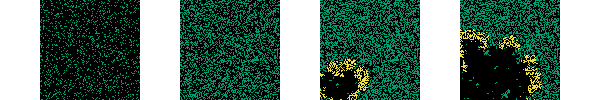
\includegraphics[width=\textwidth]{Figure 14.6.B}
\caption{Cellular automaton of a forest-fire model}
\end{figure}
\noindent % Cellular automaton of a forest-fire model
The longer that the universe stays in a supersaturated state of containing one subsystem in excess, the more vulnerable it is to a massive chain reaction initiated by the Seed of Logos. A relatively small ``forest fire'' via a crystallization event would release a relatively small amount of energy that is subsequently absorbed. If the crystallization event occurs when none have occurred for an extended period of time, it would be catastrophically large and release an enormous amount of free energy at once.

The reason for the infrequency of such catastrophe is the complexity required to reach such a supercritical state. Complexity $\mathcal C$ is a matrix defining the minimum length path from state $i$ to state $j$. We define complexity as the minimum time argument in which the adjacency matrix entry $A_{(i, j)}$ is greater than $0$:
$$\mathcal C(i, j) = \underset{t \in \mathbb N} {\arg \min} [(A^t)_{(i, j)} > 0]$$
For a finite Boolean random walk, the complexity $\mathcal C(i, j)$ is longer between two opposite planar states than between two opposite checkerboard states. 
\begin{figure}[H]
\centering
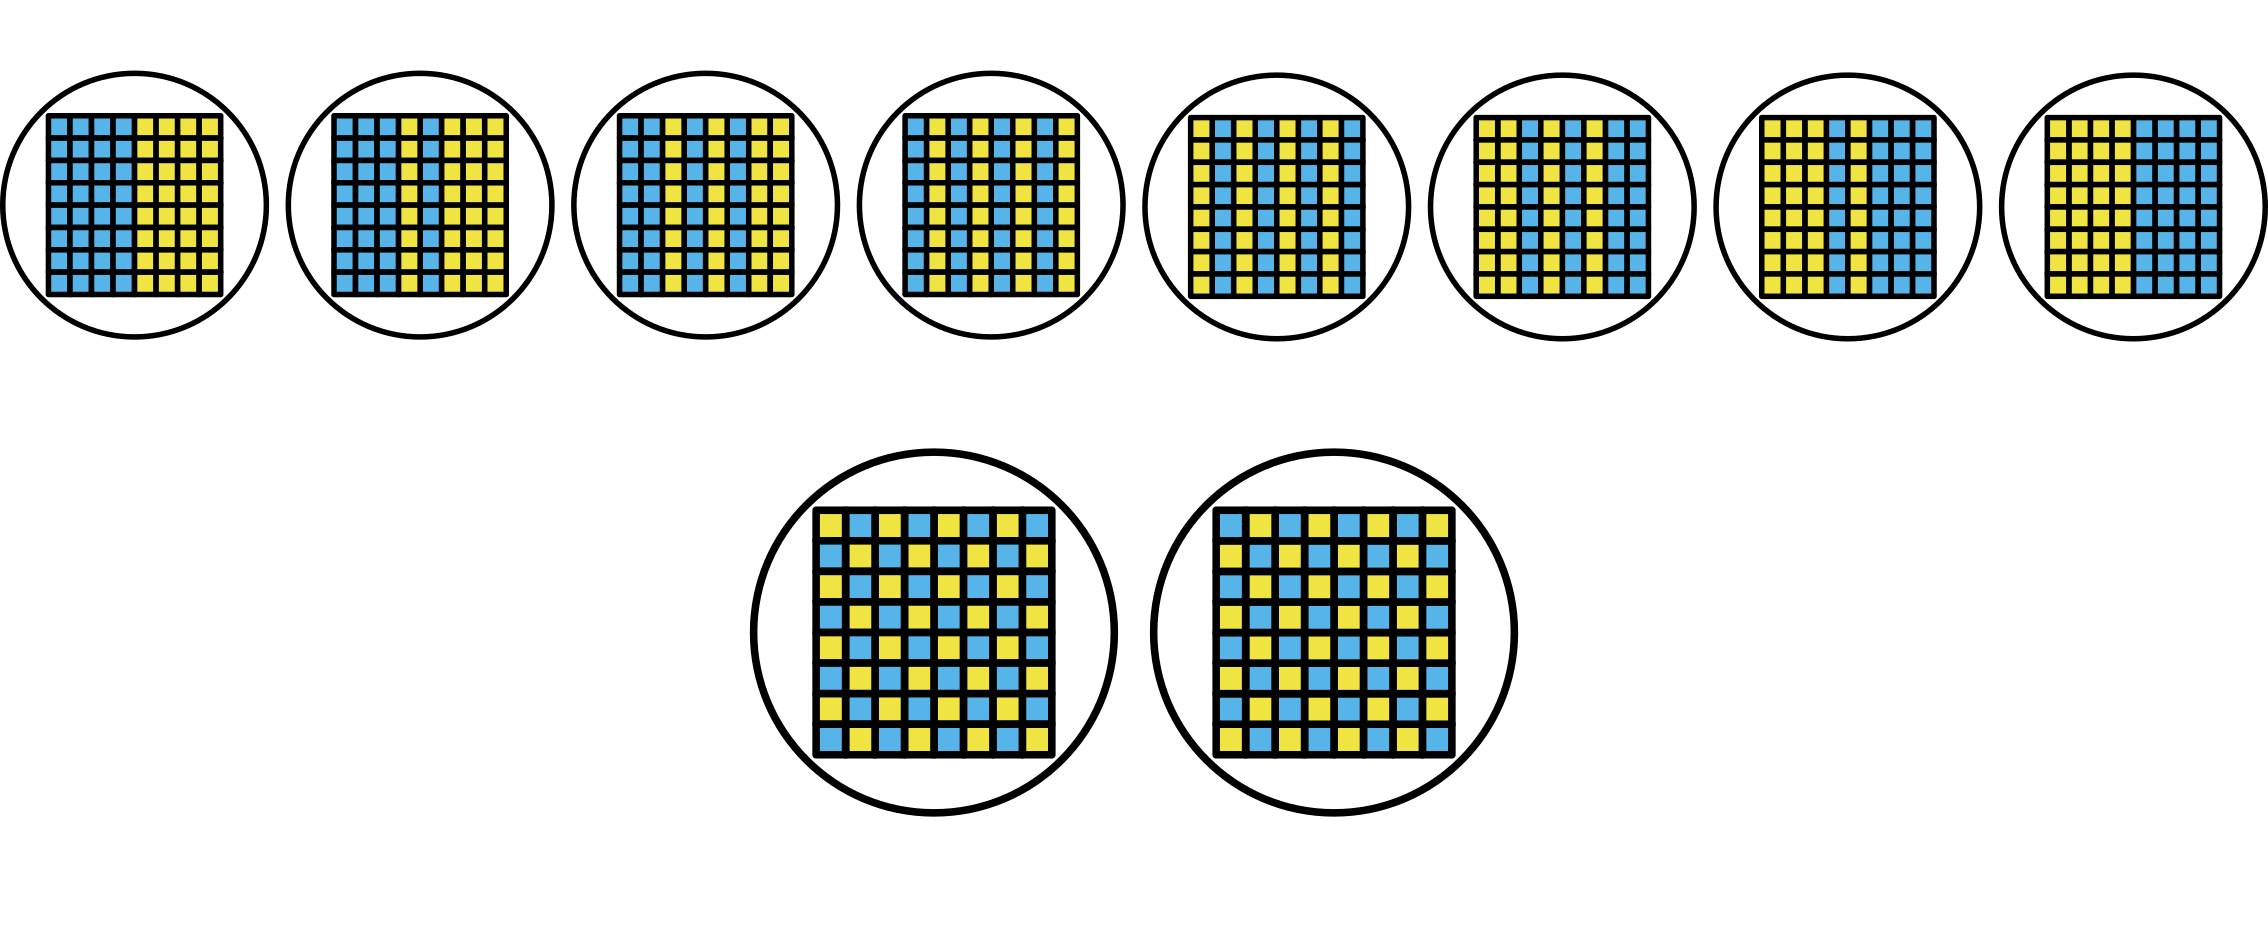
\includegraphics[width=\textwidth]{Figure 14.6.A}
\caption{The complexity between two planar states versus between two checkerboard states}
\end{figure}
\noindent % Example figure showing distance between states of a Boolean random walk
The checkerboard states have a complexity $\mathcal C$ of $1$. The planar states in the example have a complexity $\mathcal C$ of $8$. The aforementioned forest-fire model has a high complexity until it reaches the supercritical state. The same can be said for the hypothetical \textbf{Seed of Logos} which requires the universe to appear ``dead'' before the seed revives it.

But what is the actual configuration of the \textbf{Seed of Logos}? It depends on the specific transition rule of the Boolean mechanical system, assuming the universe is actually discrete in time and space. Instead of looking for a specific configuration, we should be interested in the general properties of such a state. If the system operates under some Euclean norm or $2$-norm, we may be interested in a state whose particle count measure rapidly increases according to radial symmetry.

If we consider the current understanding of the Big Bang and forest fire models, it would make sense to look for a particle whose particle count increases by a $(d-1)$-sphere for a $d$-dimensional system. This is because the interior hollows out as it expand radially. The ash it leaves behind could be very different subsystems in comparison to the seed itself.

\section{Gravity and Relativity}
General relativity is the geometric theory of physics regarding how time and space are related. It describes how massive objects curve the paths that other particles and waves take, including light. It also describes how the time experienced by an object experiencing gravity is slower than a gravity not experiencing gravity. Likewise, an object experiencing drastic changes in acceleration experiences time slower than an object that does not.

General relativity describes gravity for continuous and deterministic systems. While it is a perfectly apt description of how objects move throughout space at large scales, it does not describe the fundamental randomness by which the universe operates at small scales. Quantum mechanics properly describes all of the fundamental forces at small scales \textit{except} gravity. What fundamental mechanism accurately describes gravity at all scales?

Gravity is difficult to reconcile in quantum mechanics since there is no evidence for a quantum of gravity, known as a graviton. There needs to be an exact mechanism for which information about gravity is communicated, yet it seems that a quantum of gravity would cause a jump discontinuity in the momentum distribution of another particle. Addressing this jump discontinuity is problematic in the same way that a Wiener process is continuous everywhere but differentiable nowhere. Gravitons are theoretically difficult to detect even under the best conditions, yet the influence of gravity is quite obvious. The momentum discontinuity a graviton causes should be even more obvious.

Gravitational waves are radially symmetric and travel at the speed of light/information, and the magnitude of information that they carry decays according to the inverse squared distance from the source. In a $3$-dimensional physical system, the force of a single gravitational pulse stays constant as the area of a sphere expands. However, the information carried does not decay after it ``strikes'' an object containing mass. Gravity does not interact with the surface of an object only. If a gravitational wave from the sun hits one side of the Earth, it will persist through to the other side of the Earth.

Gravity mirrors the simple stochastic cellular automata (SSCA) with critical parameter $\varepsilon_c = \frac{1}{2}$, and it likely mirrors other computable universes with critical behavior.\footnote{Critical parameters maximize the signal correlation for a Bernoulli random variable on a single cell.} Information does not decay simply because it interacted with a surface: The magnitude of the signal merely dispersed along the surface of a $(d-1)$-sphere for a $d$-dimensional SSCA. Check \textit{\S 5.5 Simple Stochastic Cellular Automata} to see how changing noise parameter $\varepsilon$ to different values changes the signal correlation of the system, and see \textit{\S 4.6 Ising Model} for how the radial influence of a cell can change with the temperature parameter $T$. Cross-reference with \textit{\S 11.5 Boolean Thermodynamics} for how inverse temperature $\beta$ can dynamically change.

Every mainstream theory of gravity in the present fails to be calculable because of the presumption of continuous space. Even if gravitation is quantized, continuous time and continuous space would make calculations impossible because there is no limit on the energy or momentum that may be contained in a finite region of space. Even a simple assumption like ``No frequencies exceed the Planck frequency'' would fundamentally change how physics is conceptualized in the present. Such an assumption is equivalent to the discretization of space due to its relation to Nyquist frequency. \textbf{Nyquist frequency}\index{Nyquist frequency} is the maximum frequency of a continuous signal that a discrete signal sampler can recreate without aliasing or error, and it is precisely half the frequency of the discrete sampler.

\section{Matter, Antimatter, Macroparticles}
Matter makes up the world as we know it, and the general principle of what defines its existence is that matter rejects signals passing through it easily. Matter is known to interact with the fundamental forces of electromagnetism, weak interaction, and strong interaction through discrete quantum fields. We lack evidence for gravity being defined by the graviton, the quantum of interaction.

Antimatter is matter with opposite charge and parity. Even though matter and antimatter should come in pairs, there was a small bias towards matter production than antimatter production in our universe. This is due to the lack of symmetry in how the laws of physics interact with matter and antimatter.

One of the potential reasons for matter-antimatter asymmetry is that there is a corresponding antimatter universe that was generated in parallel with our matter universe. This would mean that there is no matter-antimatter asymmetry in the universe as a whole and it is only imbalanced locally in space and time. This is the most basic theory but even direct observation would be insufficient. There must also still be a mechanism that defines local asymmetry of matter.

In the context of Boolean statistical mechanics, it would make sense for particle-antiparticle pairs of macroparticles to emerge from a ``neutral'' vacuum. These macroparticles are made of the fundamental Boolean particles or cells of the universe, but the stability in their structure should normally mean that they will not dissociate until colliding with their antithesis. Shannon's \textbf{noisy-channel coding theorem}\index{noisy-channel coding theorem} guarantees it is possible.

However, since many objects are computationally possible in a Boolean mechanical system, it is entirely possible that there is an computational object or computational process that is biased towards creating matter or destroying antimatter. It would not take a particularly large imbalance for matter to overtake antimatter. The process that created this imbalance would in theory have some sort of residual that is maintained in the vacuum, and these residuals may even be fundamental to how the vacuum works.

Depending on the actual specific transition rule of a Boolean mechanical system, it is not necessary to have matter-antimatter balances at some initial time step. Under a transition rule that does not require balance in Boolean values such as simple stochastic cellular automata, it is statistically unlikely that macroparticles necessarily form particles and antiparticles in equal amounts. In a Boolean value preserving transition rule such as Boolean random walks under balanced initial conditions, then particle bias is likely the result of what would normally be an antiparticle \textit{supporting the structure} of particles. By annexing the space around matter, this ocean of support restricts the spontaneous emergence of antimatter.

This ocean of support would be very difficult to erase if it does not directly interact with matter and is almost neutral. This would make it the ideal candidate for some, but not all, of dark matter in the observable universe. This \textit{dequantized antimatter} would not have sufficient energy to annihilate our regular quantized matter, and it would be difficult to detect using our primitive method of shooting a particle really fast with another particle. The push and pull would be extremely subtle, but it would make objects appear heavier than they really are. This mass difference would be especially noticeable in networks with a topological dimension of approximately $1$ but a Hausdorff dimension of approximately $2$.

One of the most important properties of dequantized antimatter is that it generally resists requantizing into quantized antimatter. The requantization energy in a vacuum is likely much higher than the energy needed to make a particle-antiparticle pair. In contrast, the dequantization process may have only been possible during early stages of the universe. It would take a special environment to combine dequantized antimatter into its original form. Dequantized antimatter may or may not exist, but the way that they might interact with matter might be worth theorizing.

For example, \textbf{quantum vortices}\index{quantum vortex} may occur in superfluids and superconductors. These vortices are \textbf{topological defects}\index{topological defect} in the flow vector field. It is entirely possible to have \textit{fractional vortices} along the grain boundaries of the superfluid or superconductor. A polycrystalline material has many smaller crystals inside of it, and these crystallites are regular in their domain and have a sudden phase shift between regions.

The exterior of a dequantized antimatter would be difficult to determine. Other than the question of whether or not it is reasonable to assume that dequantized antimatter exists in the first place, the actual structure that it must take is cannot be determined by the assumption of existence. It could either be some sort of stable fractional antimatter similar to fractional vortices or it could be more fluid and continuous.

\section{Vacuum and Zero-Point Energy}
The vacuum is the absence of a particle in a region of space, and a particle is a uniquely stable structure in a quantum field. Even in the absence of a particle in the vacuum, it naturally fluctuates and proposes different values in this field. When a quantum system is in the lowest possible energy state, it is said to be at its zero point energy.

If we think of an closed physical system as behaving according to a Markov chain with respect to particle counts, the zero-point energy state has a way to fluctuate to different values due to the uncertainty principle. Let us suppose that particle counts may be unbounded and approximated with the half-normal distribution. Like a Wiener process, assume that the standard deviation $\sigma$ of a Normal distribution scales with time $t$:
\begin{figure}[H]
\centering
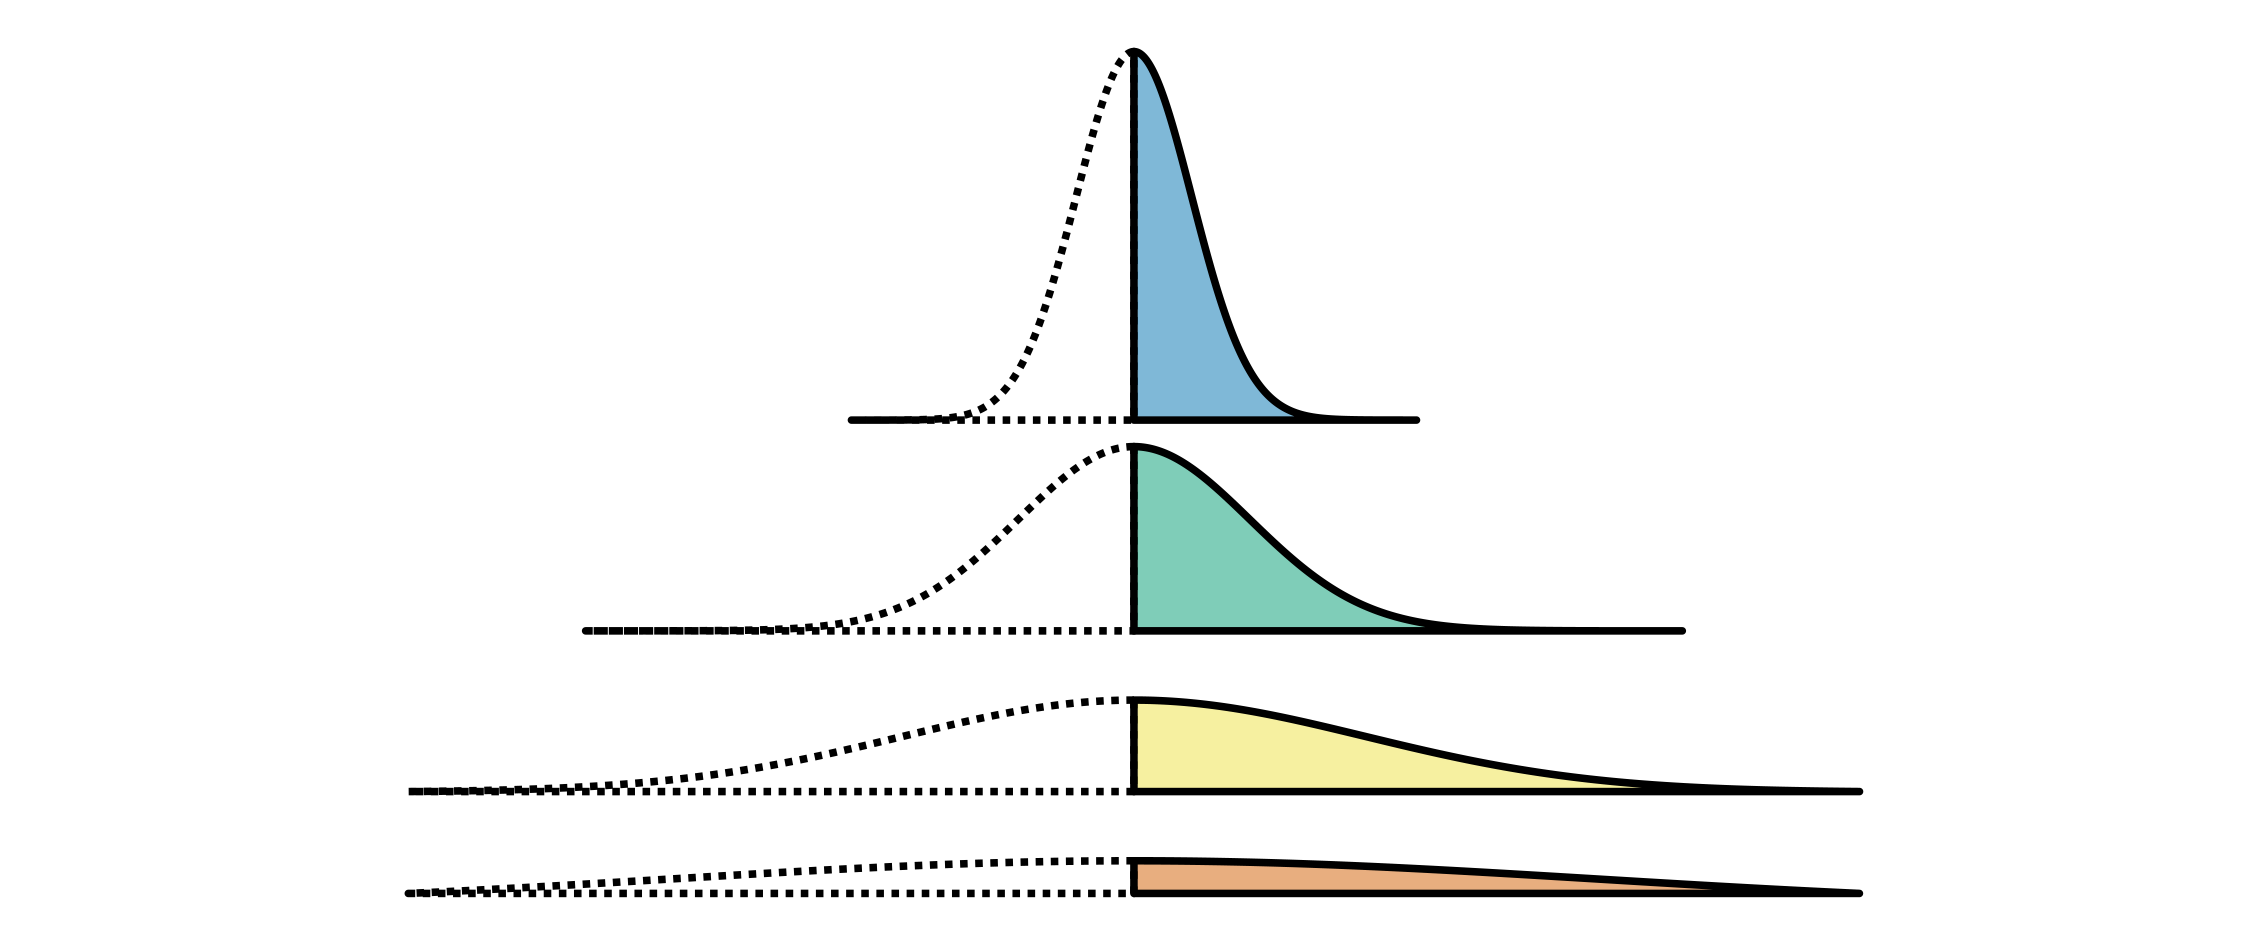
\includegraphics[width=\textwidth]{Figure 14.9.A}
\caption{Unbounded Markov models of particle generation or energy levels will tend towards infinity}
\end{figure}
\noindent % Half-normal distribution
Under this toy model, the average number of particles would tend towards:
$$ \bigg[ 2\int\limits_{-\infty}^\infty \frac{1}{\sqrt{2 \pi \sigma^2}} e^{-\frac{1}{2}(\frac{x}{\sigma})^2} dx \bigg]_{\sigma = t}= \frac{\sigma \sqrt 2}{\sqrt \pi} \bigg|_{\sigma = t}$$
Even if it were to diffuse to higher particle counts very slowly, it would have an average that tends towards infinity. 

Since the energy contained within a volume can fluctuate, so can the average number of particles. Markov models of energy are flawed if there is no maximum energy limit. There must exist a unique way to prevent the average energy of a finite system from increasing beyond a certain point, therefore preventing the average number of particles from tending towards infinity. It is possible to define a stochastic matrix $P$ with a stationary distribution $\pi$ that is non-uniform, such as:
$$P =
\begin{bmatrix}
0.4 & 0.6 \\
0.2 & 0.8
\end{bmatrix}
$$
The stationary distribution $\pi = (\frac{1}{3}, \frac{2}{3})$ means the system spends twice as long in the second state as the first state on average.

What prevents the vacuum from containing, on average, of an infinite number of particles per unit volume? Consider the Casimir effect:
\begin{figure}[H]
\centering
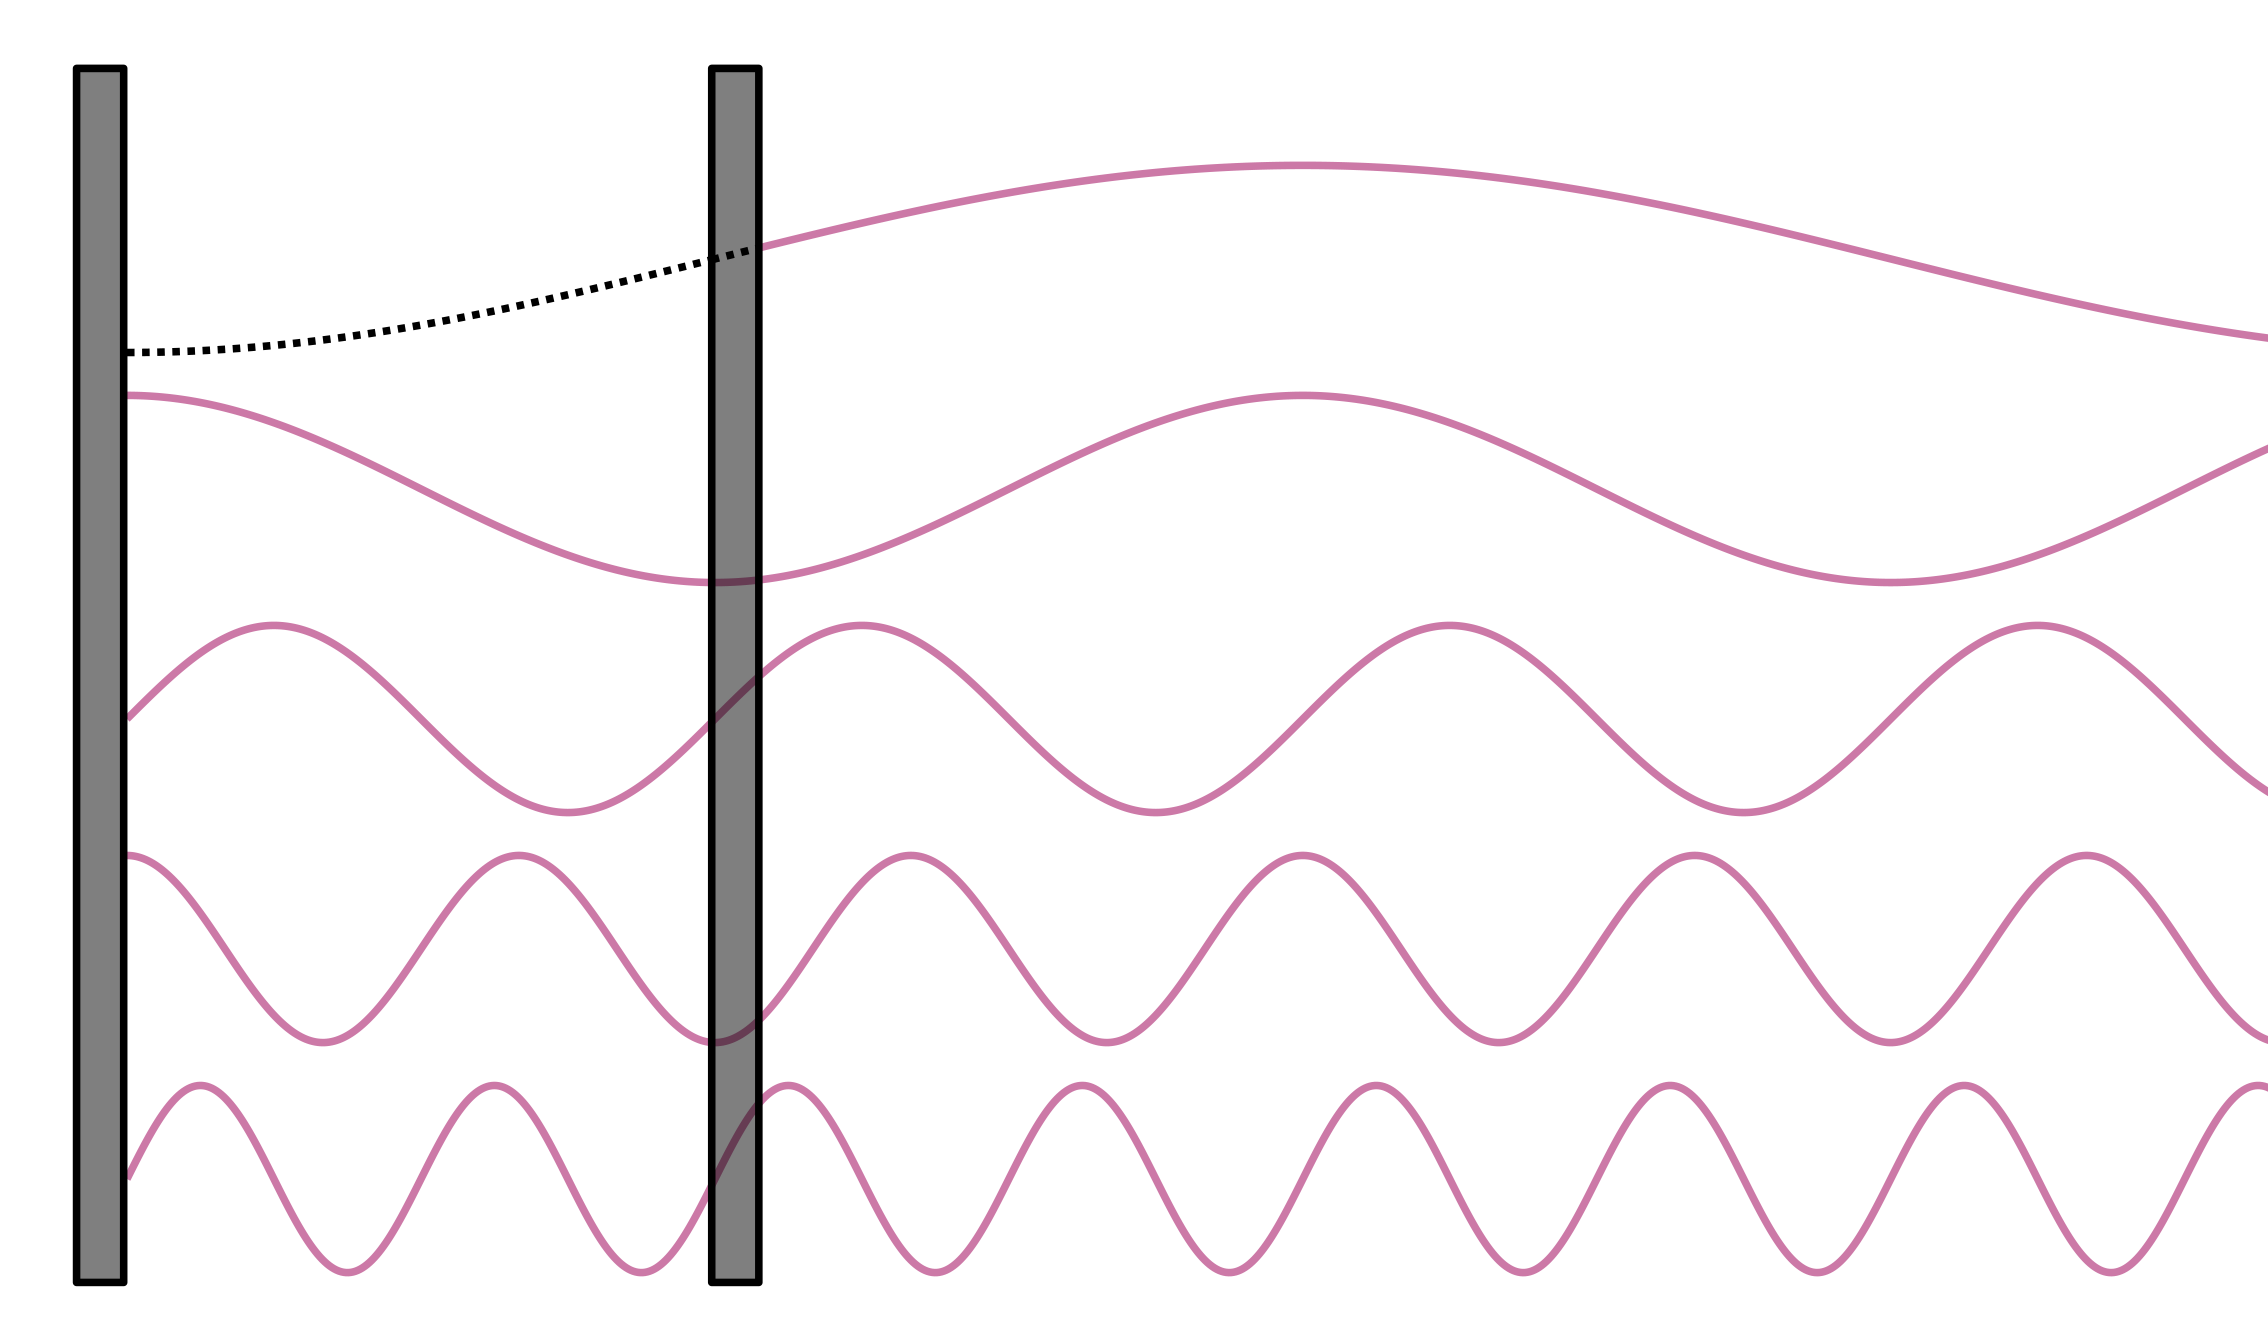
\includegraphics[width=\textwidth]{Figure 14.9.B}
\caption{Parallel plates in a vacuum disallow low frequency oscillations between them, creating a low pressure zone}
\end{figure}
\noindent % Casimir effect
A pair of parallel plates would experience more external pressure than internal pressure. This due to the thin region between between the plates being unable to host long wavelength vacuum fluctuations. The vacuum interior to the plates can only represent all wavelengths shorter than the distance between the metal plates, but the vacuum exterior to the plates can represent all wavelengths. In essence, the dynamics of a larger system cannot be represented by the dynamics of a smaller system.

Zero-point energy means an electron with zero velocity placed in a electrically neutral vacuum will randomly move in the vacuum due to zero-point energy. This is because there are imbalances in the electromagnetic field in the form of vacuum fluctuations on each side of the electron. These vacuum fluctuations have an average energy of $\frac{\hbar}{2}$.

Zero-point energy is applicable in Boolean statistical mechanics under the Copenhagen interpretation: A cell randomly according to some transition rule may also randomly change its value between transitions. If you consider Boolean random walks, a random walker does not need ``external energy'' to move. It is in its nature to move. Even if a transition rule is not Boolean random walks, it is worth considering the degree by which they differ. Zero-point energy is a local property, having no intrinsic meaning in the Markov chain representation.


\section{Why Three Dimensions}
What is special about $3$-spatial dimensions for a computational theory of the universe? If we recall that time is another dimension, then we have a total of 4 dimensions. Two ideas that make 3D special: the \textbf{axiom of constructibility}\index{axiom of constructibility} and the unique properties of \textit{4-dimensional manifolds}. The axiom of constructibility is how we claim that an infinite amount of Boolean cells may make the continuum via the \textit{continuum hypothesis}. The unique properties of 4-dimensional manifolds mean that there is no computable property to tell if two manifolds may deform into each other, and classifying all 4D manifolds would solve the \textit{Halting problem}.

What can we intuit about these ideas? A Boolean mechanical system with dimensions of $3$-space, $1$-time and assumes the axiom of constructibility creates a 4D continuum that likewise assume the strange properties of 4D manifolds. A deeper dive into the nuance of higher-dimensional topologies is better described by other authors in their works.

\section{Arguments For and Against Boolean Mechanics}
What makes Boolean statistical mechanics a useful idea? The primary idea is the way that it relates computable functions to restrictions on permutations of the universe. It is a very general theory for how the universe could work and how complexity emerges from simple rules and structures. This means that our understanding mathematics, statistics, computer science, and linguistics are applicable to the physical world in a more fundamental way than physics.

What are some possible ideas to reject Boolean statistical mechanics? The main idea is that relying on the generality of computing is quite ugly. It does not state anything specific about how the universe currently works, only how it can work assuming it is discrete or discretizable. Due to the \textbf{word problem}\index{word problem}, there exists is no finite algorithm to decide the equivalence of all statements between computable universes. This means that it is not possible to reverse engineer an absolutely true framework about the universe without bias from the method of determination, confounding empiricism. Any theory of Boolean statistical mechanics whose transition function obeys similar thermodynamic principles as another transition function cannot be distinguished as more or less true than another, confounding rationalism. 

The most important part to decide is on a transition rule's local channel capacity $C$ and the local transmission rate $R$. This is where simple stochastic cellular automata combined with axiom of constructibility shines: They can directly modify the local channel capacity. Since the \textbf{noisy-channel coding theorem}\index{noisy-channel coding theorem} does not address the case in which $R = C$, this is perhaps the critical threshold in which whether a data transmission being error-free is subjective per receiver.


\chapter{Relation to Other Theories}
A discrete evolution of spacetime is a model that is explicitly avoided by the physics academia at large. Worldly attachments such as funding, tenure, social and academic credence reveal the cowardice of human nature. The most damning reason why intellectuals stick to mainstream theories is shame, the negative emotion caused by deviation from cultural norms. The career risk to those who would consider a theory of discrete time and space is great, but the cognitive dissonance of being ostracized by contemporaries is greater. One need only look at the fate of Boltzmann and Ehrenfest to see how valiantly struggling to understand a subject, only to be ridiculed, might cause scientists to turn their backs on the principles of intellectualism.

Boolean random walks is a lattice gauge theory which conserves the total number of particles and antiparticles in the simulation. Even if some transition function for Boolean statistical mechanics does not conserve some property, we claim that eigenclasses of states result in conserving some gauge \textit{on average}. Conservation laws are merely the tendency to stay in the same class. If BSM underlies reality, weak communication between classes would make conservation laws the normative perception.

Analyses of lattice gauge theories often describe the conservation of crystal momentum $\hat p$ and conservation of energy $\hat H$. The Brillouin zone of this reciprocal lattice contains all the information needed to describe the state of the system due to corresponding to the \index{Nyquist frequency}\textbf{Nyquist frequency}.

Hamiltonian lattice gauge theory discretizes space but not time. \textbf{Bloch's theorem}\index{Bloch's theorem} of wavefunctions on a crystal lattice states that continuous wavefunctions on it need only be expressed in terms of crystal lattice eigenstates up to the maximum frequency of the crystal's points. A lattice's position basis $| \hat x | \phi \rangle$ has a reciprocal lattice in the momentum basis $| \hat p | \phi \rangle$.

Spin networks are dual to Hamiltonian lattice gauge theory as the linear combination of spin network eigenstates. Spin networks have spawned a plethora of adjacent theories rooted in graph theory: Particles are vertices and force carriers are edges of a graph. On a lattice, the link between two points is called a Wilson line, and four links about a single square form that lattice's smallest Wilson loop. This square, called a plaquette, forms the basis of loop quantum gravity.

\section{The Standard Model}
No discussion about successor theories is complete without addressing issues in the most successful theory of the present. The Standard Model of quantum mechanics posits a set of particles that describe three of the four fundamental forces: electromagnetism, the weak force, and the strong force. Gravity is the big mystery missing force that is not explained particularly well in the model. This is due to a lack of evidence for a discrete force carrier of gravity, referred to as a graviton.

Consider the following thought experiment. Two electrons set at a distance $d$ apart are trapped in approximately linear potentials:
\begin{figure}[H]
\centering
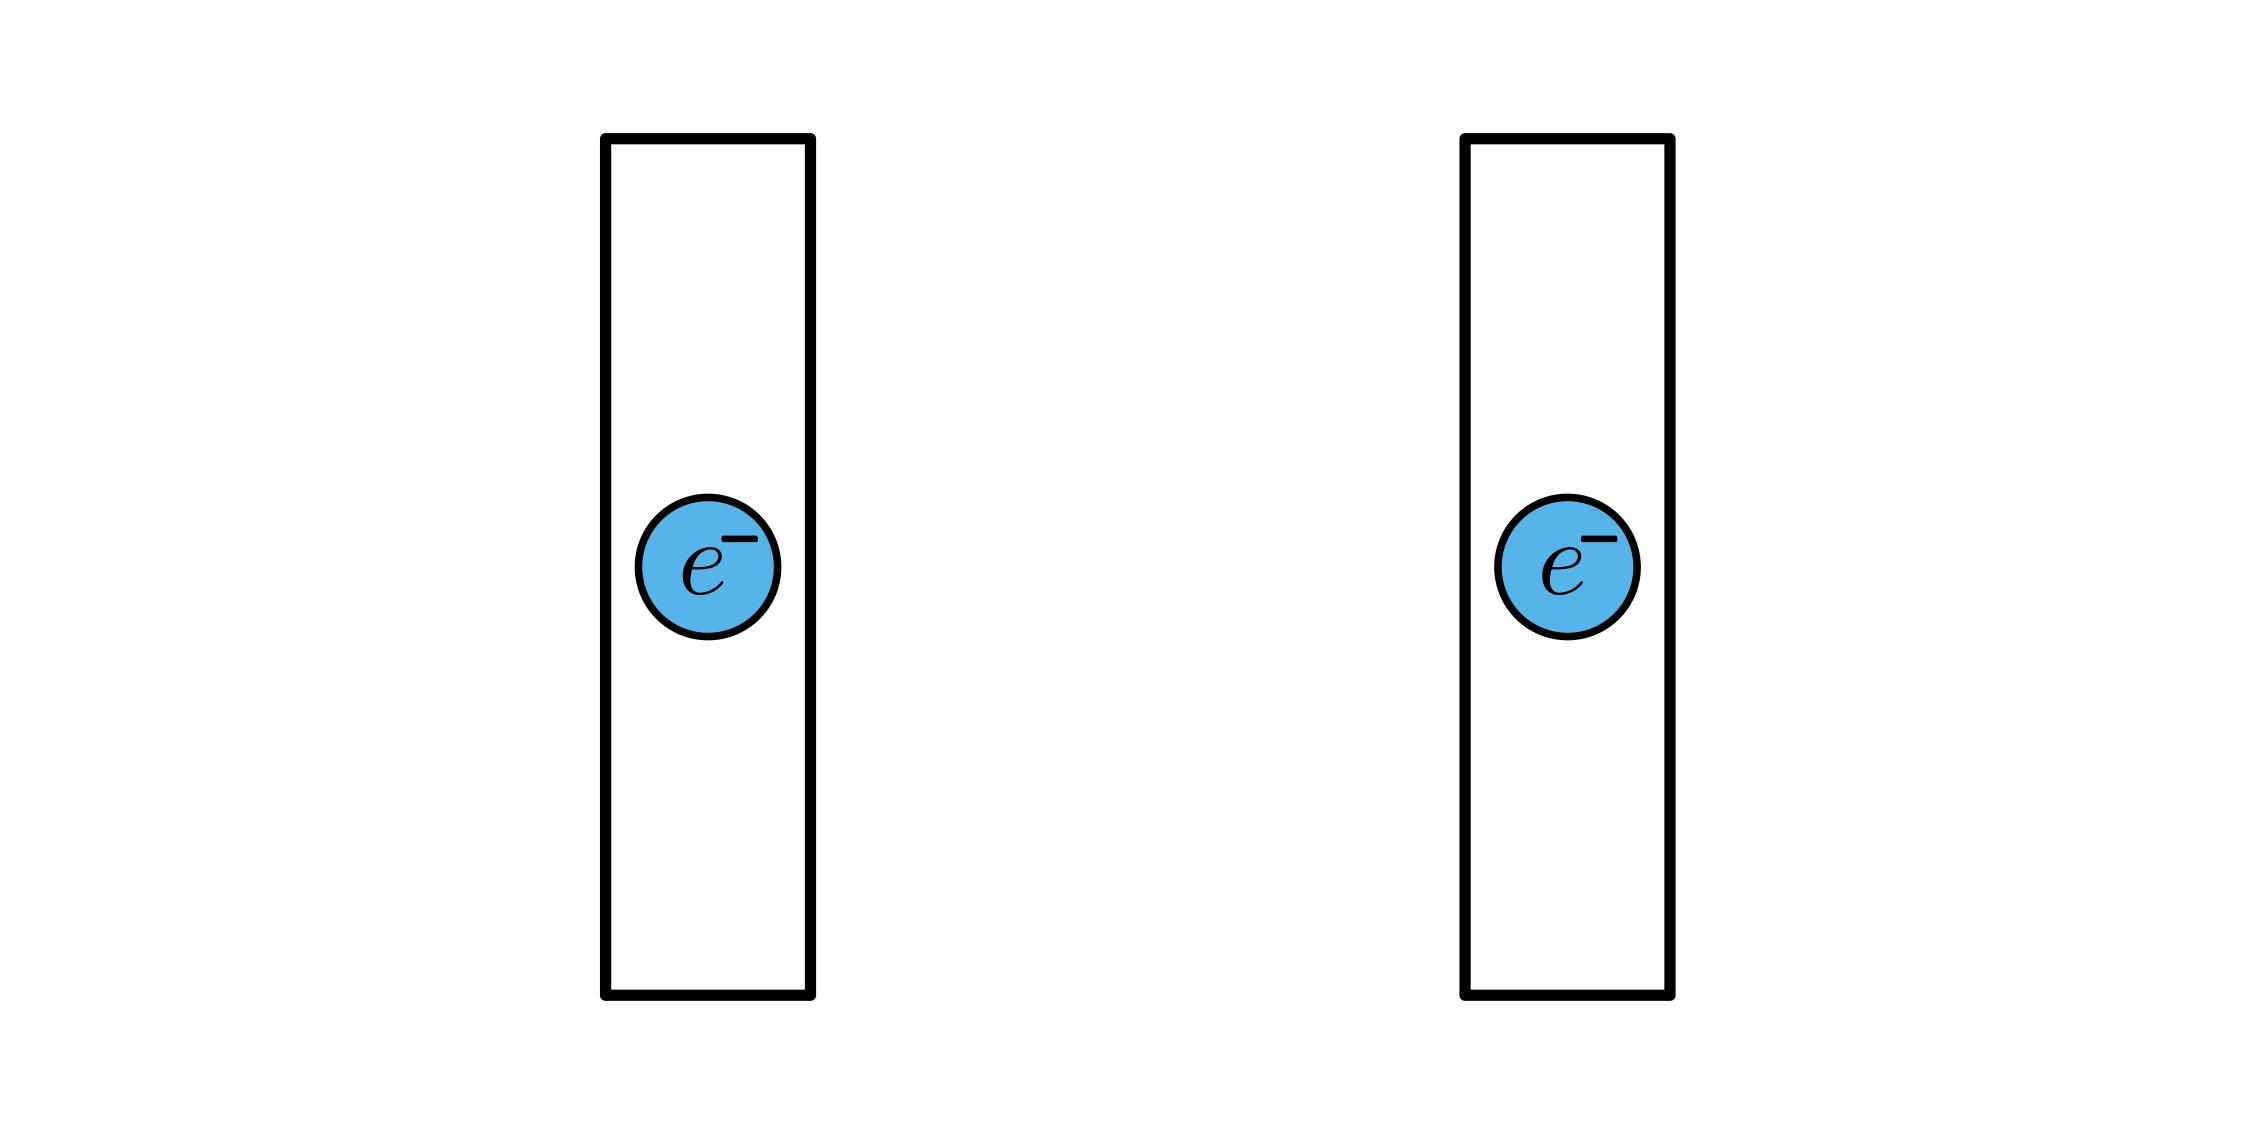
\includegraphics[width=\textwidth]{Figure 15.1.A}
\caption{Electrons trapped in massless cylinders}
\end{figure}
\noindent % Electrons in cylinders
As time passes, the wavefunction governing the position of the electrons will asymptotically diffuse along the potential until the probability is roughly uniform. The electrons will exert a finite amount of attractive force upon each other due to their gravity and a small amount of repulsive force due to their electric charge, and we assume that the device creating the linear trap has a mass of zero. If gravity were to pull these electrons together, then how does it act while their position is undefined or uncollapsed? The negligible mass traps would be pulled along by the electron it contains, and it may be pulled linearly, top-biased, or bottom-biased.

The Standard Model does not claim the existence of gravitons, an elementary particle that communicates gravity's signal for the gravity force field. Gravity is weak, weaker than the weak force, and is of seemingly infinite range. Gravity's mechanism is hard to verify for almost any possible theory due to its low magnitude, especially in the presence of other nearby forces. How does gravity work at short distance when the other forces have strong signal interference?

Fermions are quantum particles that make up most of what we call matter, or objects, because they reject information communicating through their interior. This fundamentally includes copies of themselves. Bosons are quantum particles that act as information packets or signal carriers between fermions, and they may overlap with themselves via constructive and destructive interference. Fermions are half-integer spin systems $\{\frac{1}{2}, \frac{3}{2}, \frac{5}{2},...\}$ corresponding to $e^{2\pi i (n+\frac{1}{2})}$ for $n \in \mathbb N$. In contrast, bosons are integer spin systems $\{0, 1, 2,...\}$ corresponding to $e^{2\pi i (n)}$ for $n \in \mathbb N$. Two fermions may add or subtract their combined spins to form a bosonic system. Therefore, a composition of any number of bosons and an even number of fermions is a boson overall. The further away we are from the convex hull encapsulating the particles, the more computationally indistinguishable the system is from a boson.

\section{Boolean Mechanics as Lattice Gauge Theory}
A \textbf{gauge theory}\index{gauge theory} is a field theory whose dynamics do not change under local transformations. In general, a field theory is a complex-valued function $f$ and a transformation $R$ such that it maps $f \rightarrow R f = e^{ln(R)} f$. A global transformation applies the same gauge transformation uniformly to $f(x)$. A local transformation $R(x)$ may apply any gauge transformation $R$ to each point $x$. For example, the gauge theory for the electromagnetic field is given by:
$$f(x) \rightarrow e^{\theta}f(x)$$
In order to allow rotations for every point $x$, we allow the use of a local rotation function $\theta(x)$ instead of a global rotation constant$\theta$:
$$f(x) \rightarrow e^{\theta(x)}f(x)$$
Therefore, general time advancements of a gauge theory are defined as:
$$f(x,t) = R(x,t) f(x,0)$$
In comparison, a transition matrix $P$ describes a global transformation $f \rightarrow P^t f$ due to the state space representation.

The local transformation $R(x)$ of a gauge theory has the following restrictions via the \textbf{Cauchy integral theorem}\index{Cauchy integral theorem} of complex analysis:
\begin{enumerate}
\item Unitary: The local transformation function $R$ is unit magnitude for all $x$.
$$|R(x)|=1$$

\item Holomorphic: The contour integral of gauge over any simple closed curve $C$ is the identity matrix.
$$e^{\oint_C \ln[R(x)] dx} = e^0 = I$$

\item Entire: The net change in gauge over the whole simply connected domain $\Omega$ is the identity matrix.
$$e^{\int_\Omega \ln[R(x)] dx} =e^0 = I$$
\end{enumerate}
These restrictions state that the transformation $R$ does not change the overall value of the field, but instead moves things around. The entire function restriction is an extension of the holomorphic condition: The summation may be decomposed into a sequence closed curves.

The transformation of an electromagnetic field is given by the unitary group $\operatorname{U}(1)$. The local transformation $R$ cannot change the overall electric charge of the field but can change its arrangement. The transformation of a quantum chromodynamic field is given by the special unitary group $\operatorname{SU}(3)$, yet the pointwise color transformation function $R$ is colorless overall. The general form is given by Lie algebras.

Boolean random walks may be considered as a primitive sort of gauge theory on a $\mathbb Z^d$ lattice. A \textbf{lattice gauge theory}\index{lattice gauge theory} is a gauge theory on a lattice.
\begin{figure}[H]
\centering
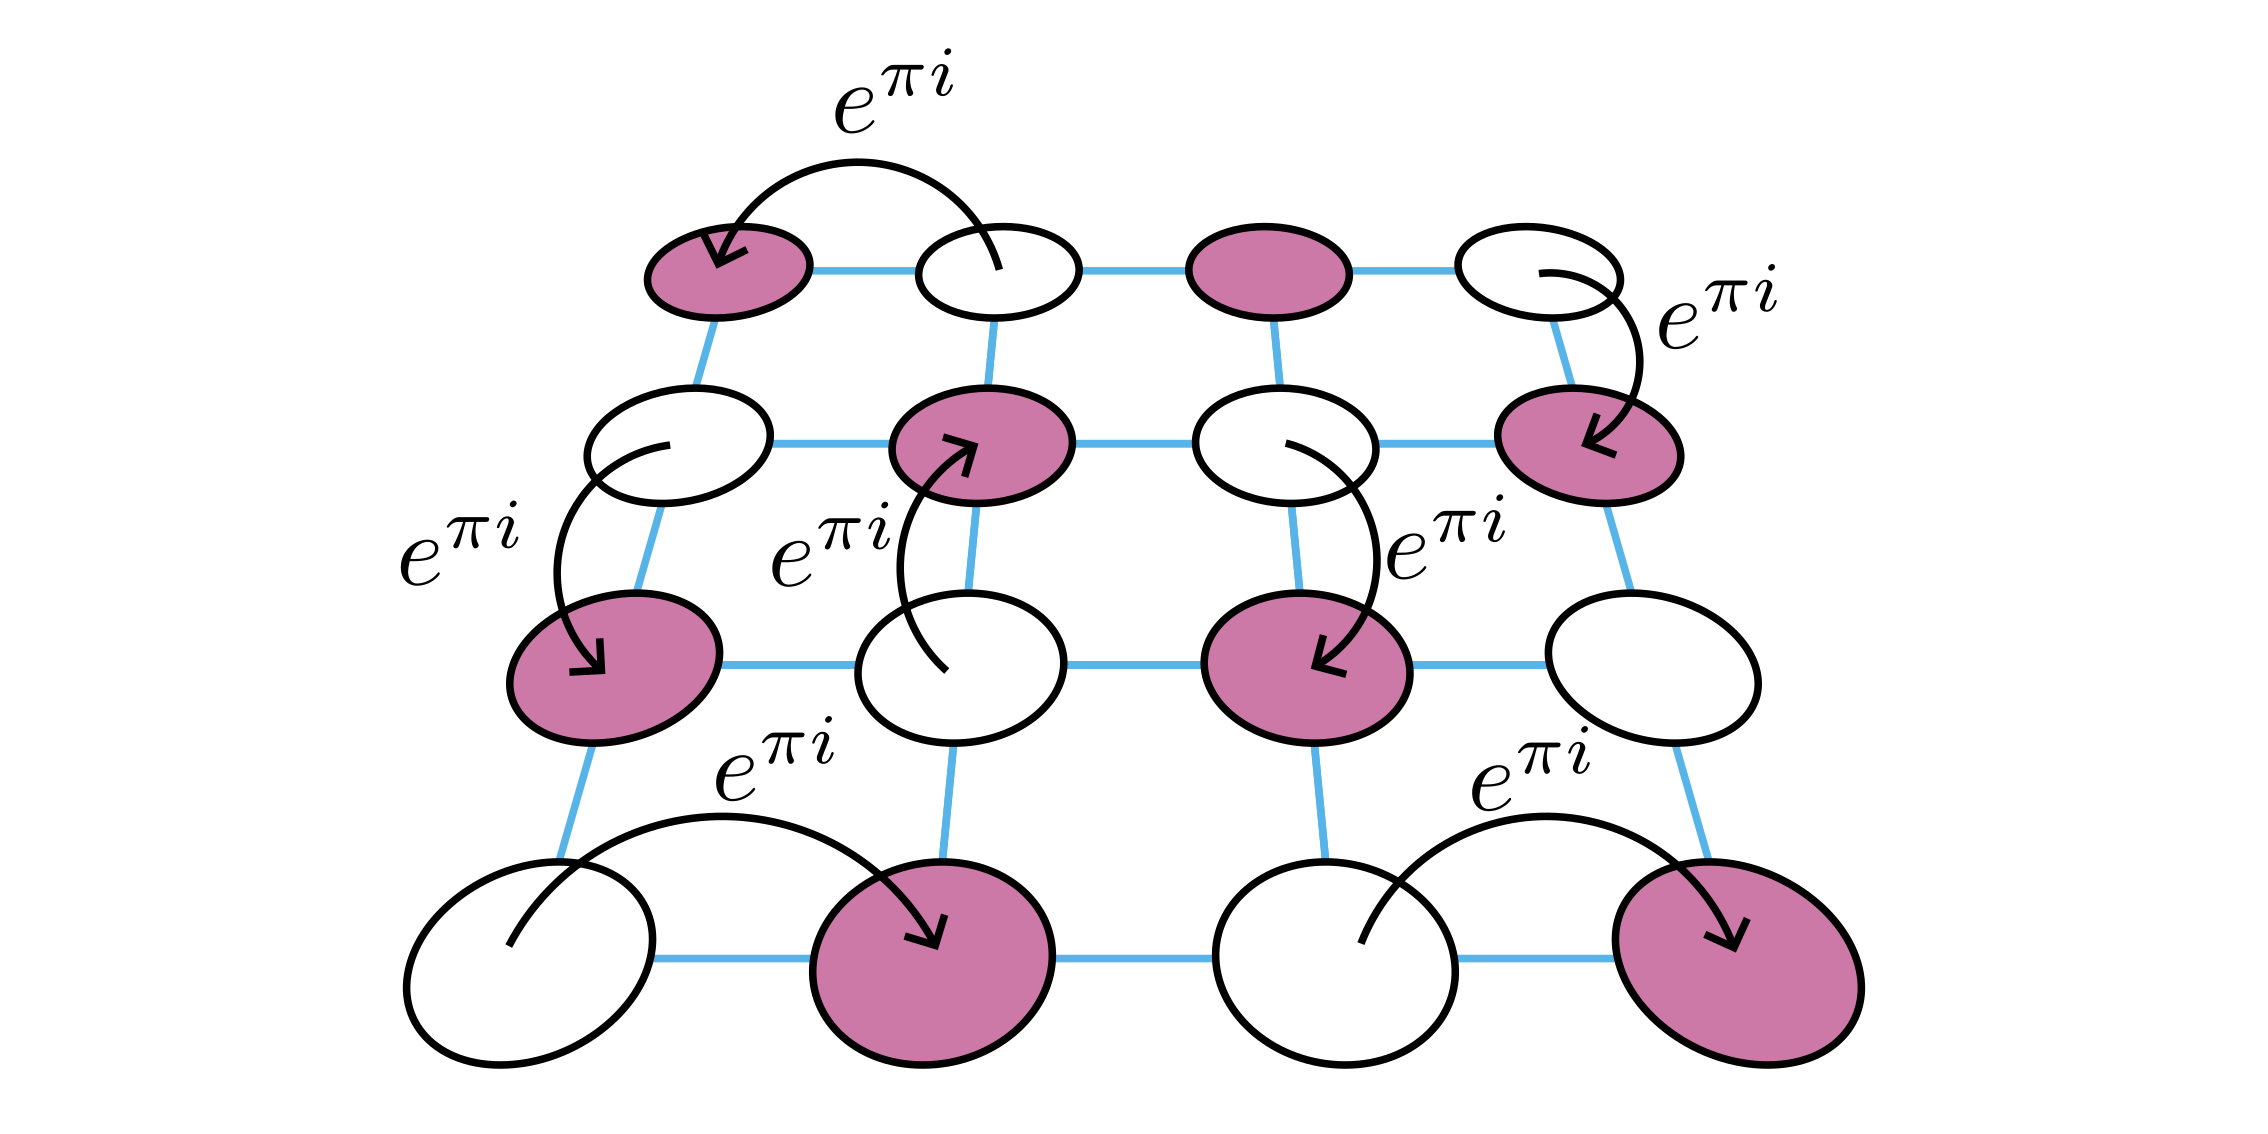
\includegraphics[width=\textwidth]{Figure 15.2.A}
\caption{Boolean random walks obeys the properties of a lattice gauge theory because any transformation is unitary, holomorphic, and entire}
\end{figure}
\noindent % BRW as a lattice gauge theory
It maintains holomorphic property of path invariance, or returning to the starting position should have the same orientation of gauge. It also maintains the entire property of gauge conservation, that the cumulative bias in orientation is conserved. For electromagnetism, that means that closed paths return you to the same phase and that the net charge of the transformation is zero. For quantum chromodynamics, that means that closed paths return to the same orientation and that the transformation overall is colorless.

Gauge theories are important because they describe how mass originates in the universe. Mass is resistance to movement or change, which is why most of the mass we perceive is cold. In Boolean statistical mechanics, this paradoxically means we may measure the gravitational effects of hot objects (dequantized antimatter) without perceiving a hot cluster of matter. Networks of forces between objects may emit more gravitation than the objects themselves, such as in the case of gluons. Galactic clusters may have more gravity than mass estimates of stars alone due to glueball streams between stars.

Physics wishes to solve the Yang-Mills mass gap for continuous spaces. An \textit{effective field theory} works at time and energy scales that ignore frequencies higher than some cutoff, and this is equivalent to discretization of time and space via the \textbf{Nyquist–Shannon sampling theorem}\index{Nyquist–Shannon sampling theorem}. The mass gap is the difference in energy between vacuum state and the lowest energy state. This mass gap is easy to prove for lattice gauge theories but unresolved for continuous gauge theories.

Even though it is proven that a mass gap exists for lattice gauge theories, most of physics does not assume the \textbf{axiom of constructibility}\index{axiom of constructibility}. Under axiom of constructibility, the Yang-Mills mass gap is trivially proven. Such a proof would still be unsatisfying to the physics community that disdains digital physics theories. Boolean random walks is perhaps the simplest lattice gauge theory for which we may observe mass and gravity through study. Due to the lack of \textit{blue skies research} in academia, the physics community may not realize the insolvability of Yang-Mills if it depends upon a choice mathematical axiom.

The Yang-Mills mass gap requires the proof of a non-zero eigenvalue between the lowest energy state and second-lowest energy state, also known as the ground state and excited state. The mass gap refers to the spectral gap, referring to the difference between the largest magnitude and second-largest magnitude eigenvalue. This definition is directly applicable to a transition matrix $P$ but flawed for periodic Markov chains. 

I revise the definition of spectral gap to refer to the difference between the eigenvalue $\lambda_1 = 1$ and the largest magnitude eigenvalue with magnitude less than $1$.
$$\xi = |1| - |\lambda_{\max}|, \quad \lambda_{\max} = \underset{|\lambda|<1}{\max}|\lambda_i|$$
According to the Perron-Frobenius theorem, a transition matrix $P$ always has an eigenvalue with magnitude $1$. The eigenvalue of the lowest energy state does not decay, and the eigenvalue of the second-lowest energy state has the slowest possible decay. We can therefore define the mass gap for a transition matrix if it represents a physical system.

The spectral gap in the energy/Hamiltonian eigenvalues as given by $e^{\frac{\partial}{\partial t}} = e^{\pi i \eta} = \Lambda$ of a stochastic matrix $P$ all exist within the unit complex disc. The spectral gap $\xi$ of a Boolean random walk approaches $0$ as the simulation size $N$ approaches infinity due to the slower mixing of a large number of states. Consider the eigenvalues of a $3 \times 3$ Boolean random walk:
\begin{figure}[H]
\centering
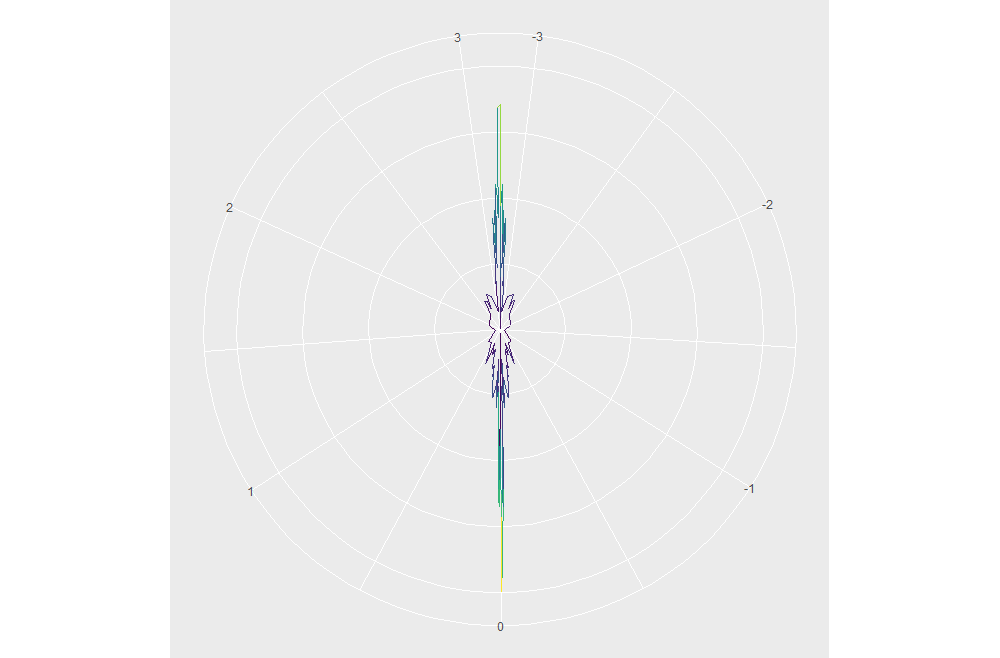
\includegraphics[width=\textwidth]{Figure 15.2.B}
\caption{Eigenvalues of a $3 \times 3$ Boolean random walk}
\end{figure}
\noindent % Eigenvalues of a stochastic matrix
Due to the small simulation size, the spectral gap is easy to detect. As humans, we classify objects due to their similarity. When we state that we can create eigenclasses due to similarity in distribution, this is derived from the fact that decaying eigenvalues imply that less normal modes are needed and that rows of the stochastic matrix $P^t$ are becoming more similar as $t \rightarrow \infty$.

Since the spectral gap $\xi$ of a Boolean random walk approaches $0$ as the simulation size $N$ approaches infinity:
$$\underset{N \rightarrow \infty}{\lim} \xi = 0$$
then the spectral gap of a continuous Yang-Mills theory can never be proven. The spectral gap of a physical theory can be found if we stop considering an \textit{effective field theory} as a flawed approximation. A better interpretation is not to cut off after some maximum frequency. Instead, we begin with some minimum wavelength and perform infinite summations of increasing wavelength:
$$\sum_{\lambda=1}^{\infty} e^{c_\lambda \pi i} f \Big (\frac{x}{\lambda} \Big)$$
Mainstream physics is attached to the idea of continuum mechanics and is cowardly in assuming the Planck length lattice mechanics as correct, despite the fact that there is no evidence that space is continuous. The assumption is that space is continuous, but there is no way to test that empirically without relying upon circular logic.

Lattice gauge theories are considered approximations of a continuous gauge theory instead of the object worth study in and of itself. The main issues with continuous gauge theories from the perspective of lattice mechanics are as follows:
\begin{enumerate}
\item Continuum approximations of spectral gap $\xi$ tend towards $0$.
\item Unconstrained transition probabilities of particle creation and annihilation.
\item Gauge transformations cannot themselves create/annihilate topological defects.
\item Proofs may depend on specific choice of mathematical axioms.
\end{enumerate}
Since \textit{blue skies research} is bad for acquiring tenure in current academic institutions, expect things to stay the same. The rise of anti-intellectualism in favor of the science of violence means that the United States will eventually be outpaced by a country with a more liberal philosophy. By then, the United States will be at the mercy of their weapons of science due to its mentally atrophied citizens.


\section{Boolean Mechanics as Spin Networks}
Roger Penrose proposed spin networks and his subsequent developments of twistor theory as a way to preserve measure properties of angles and angular momentum for discrete systems. Instead of a continuum of possible angle values, the discrete nature of combinatorics can measure large networks of discrete spin. In the limit of large networks, a continuous measure of angles can be approximated.
\begin{figure}[H]
\centering
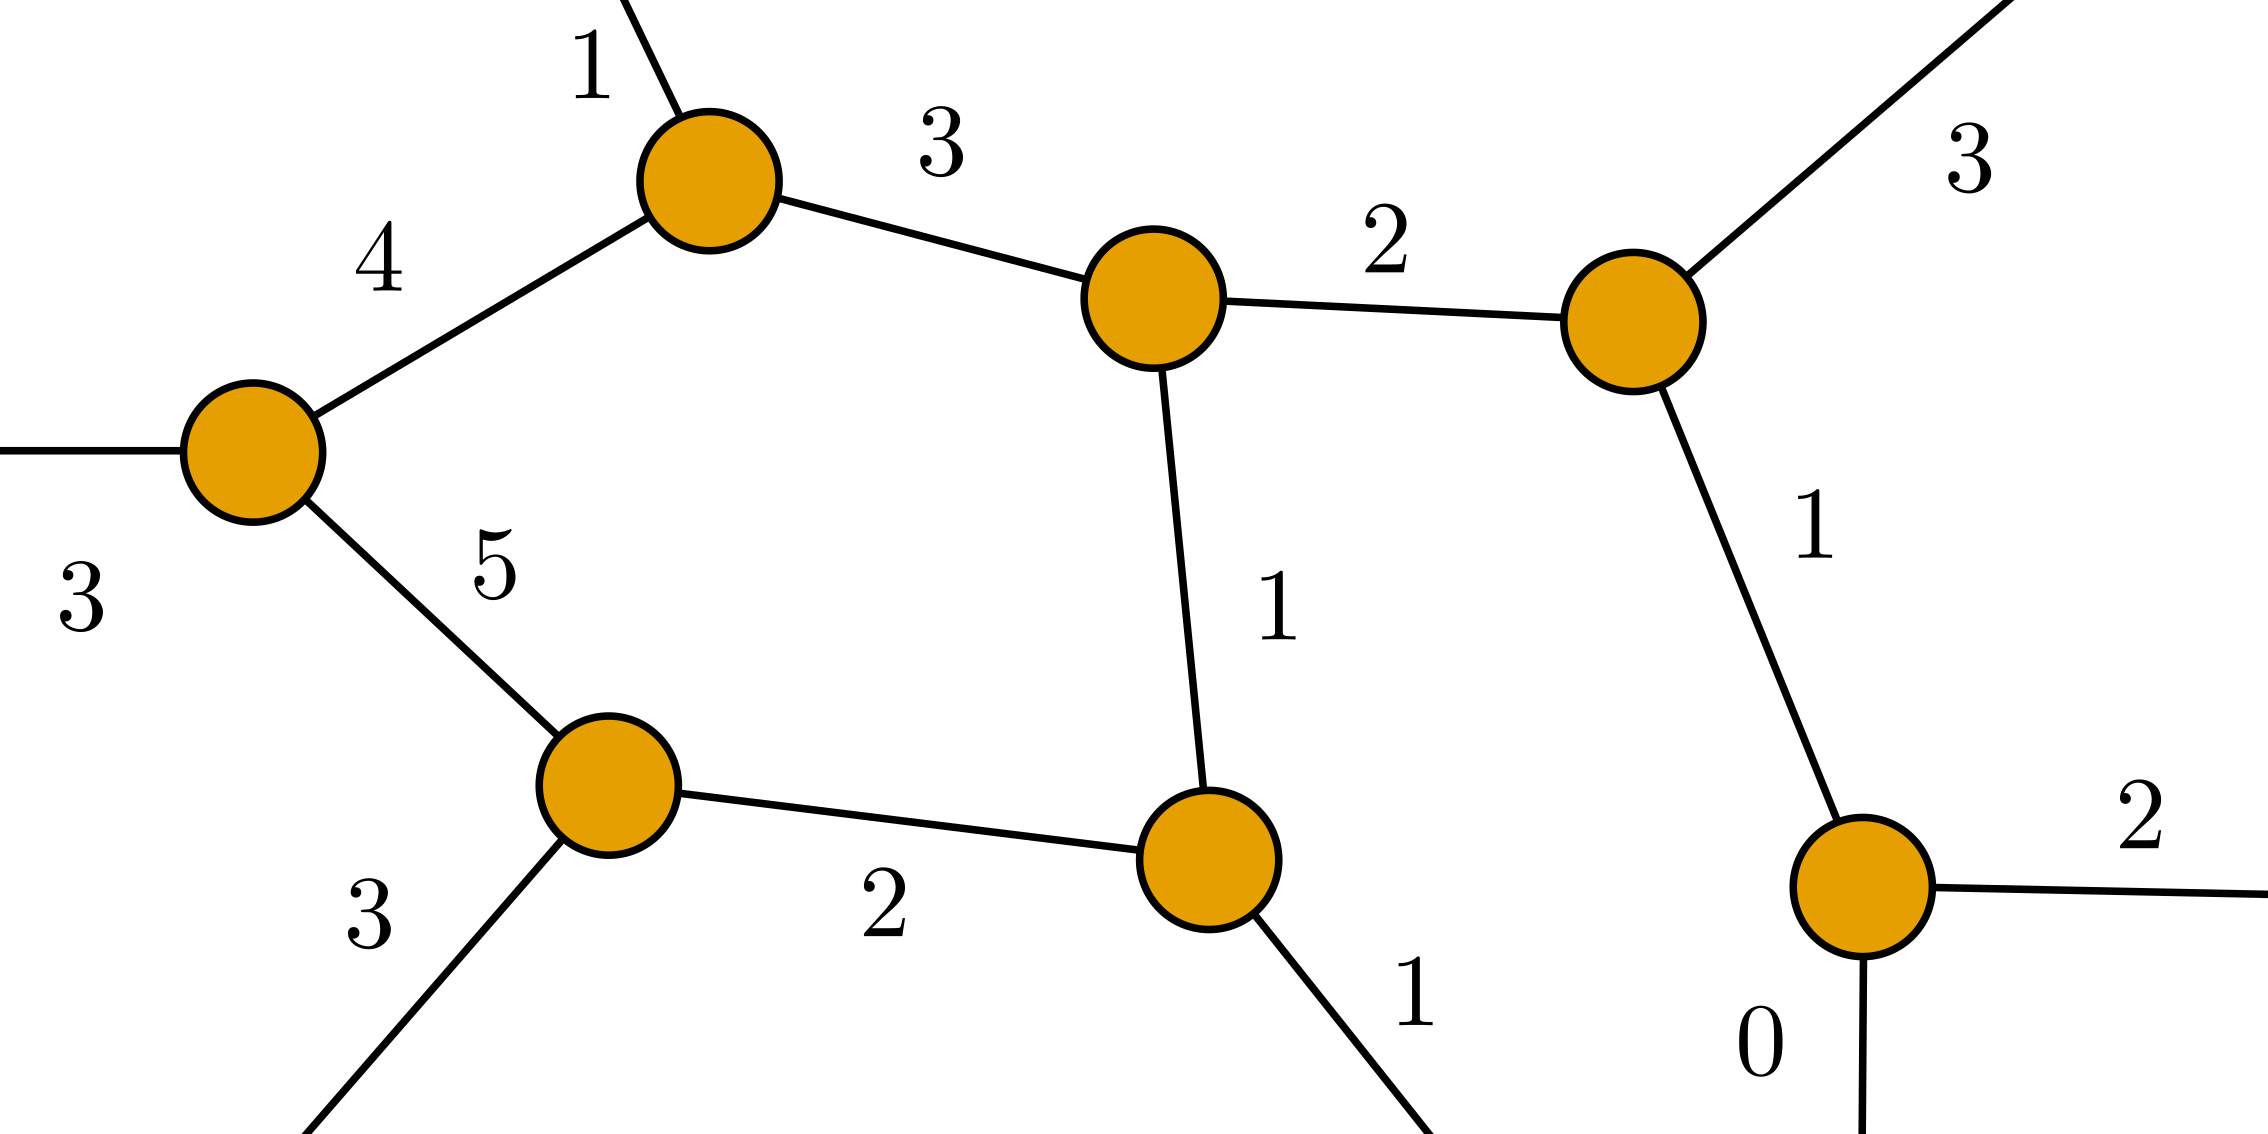
\includegraphics[width=\textwidth]{Figure 15.3.A}
\caption{A spin network diagram}
\end{figure}
% Spin network diagram
Spin networks themselves are models solved to represent transfers of angular momentum in a lattice gauge theory. Other models of spin such as spin ice, spin liquids, and spin foams trace their lineage to Penrose's original diagrams.

Each and every point represents a particle, and the incoming or outgoing numbers represent force carriers of spin$\times 2$, spin being the natural units of angular momentum $s_P = m_p \cdot \ell_P^2 \cdot t_P^{-1}$. The particle's three connecting edges form a trigram that obeys the triangle inequality:
\begin{figure}[H]
\centering
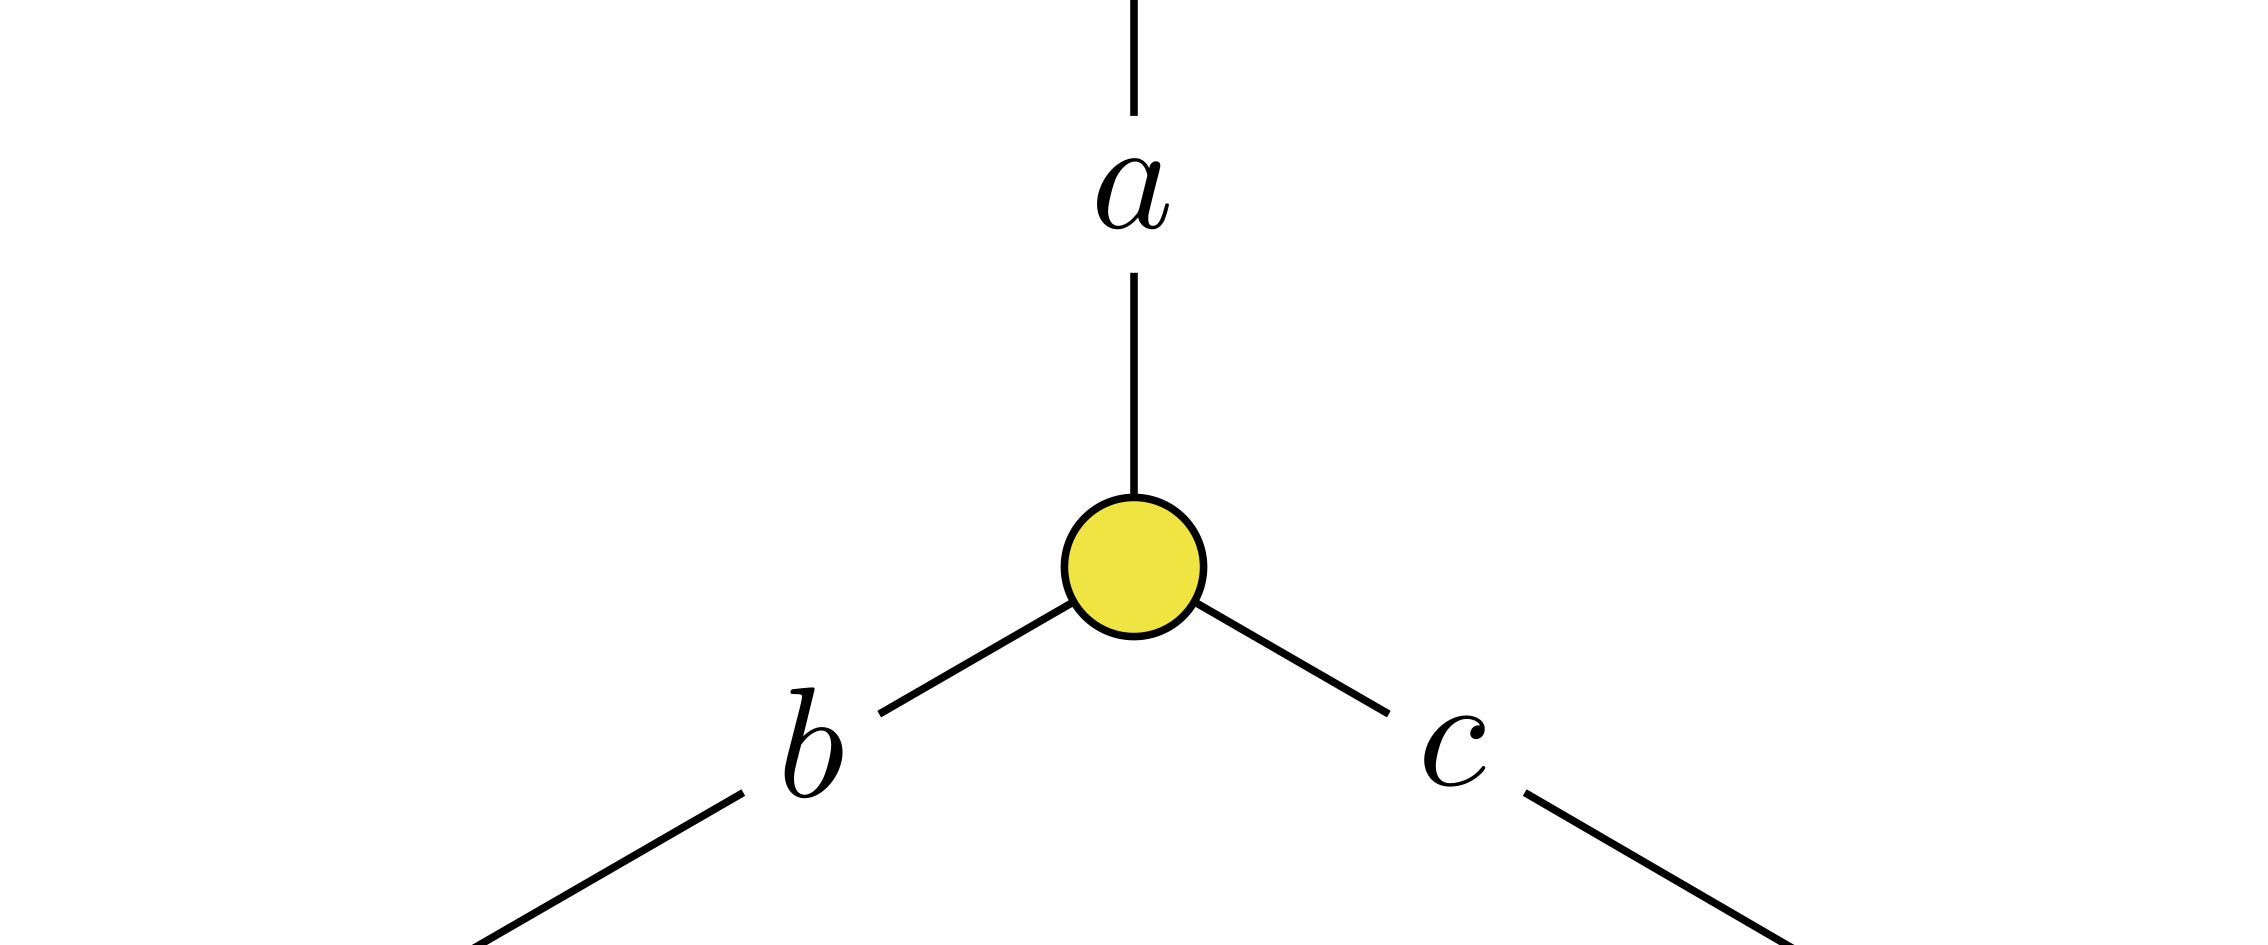
\includegraphics[width=\textwidth]{Figure 15.3.B}
\caption{The trigram of a single particle's spin transfers}
\end{figure}
\noindent % Trigram of a single particle's spin
The triangle inequality states that if $a,b,c$ are side lengths that $a \leq b+c$, $b \leq a+c$, and $c \leq a+b$. An alternative statement of triangle inequality is $a+b+c \geq 2\cdot \max(a, b, c)$. This puts a limit on the spin transfers that may occur in a system.

Another key property of spin networks is fermion conservation, or that $a + b + c$ is an even number. Any trigram or whole spin network is an abstraction representing a particle system or macroparticle. Since physical matter is made of fermions, it is important that each fermion particle does not gain or lose an odd number of spin units from a force transfer.
\begin{figure}[H]
\centering
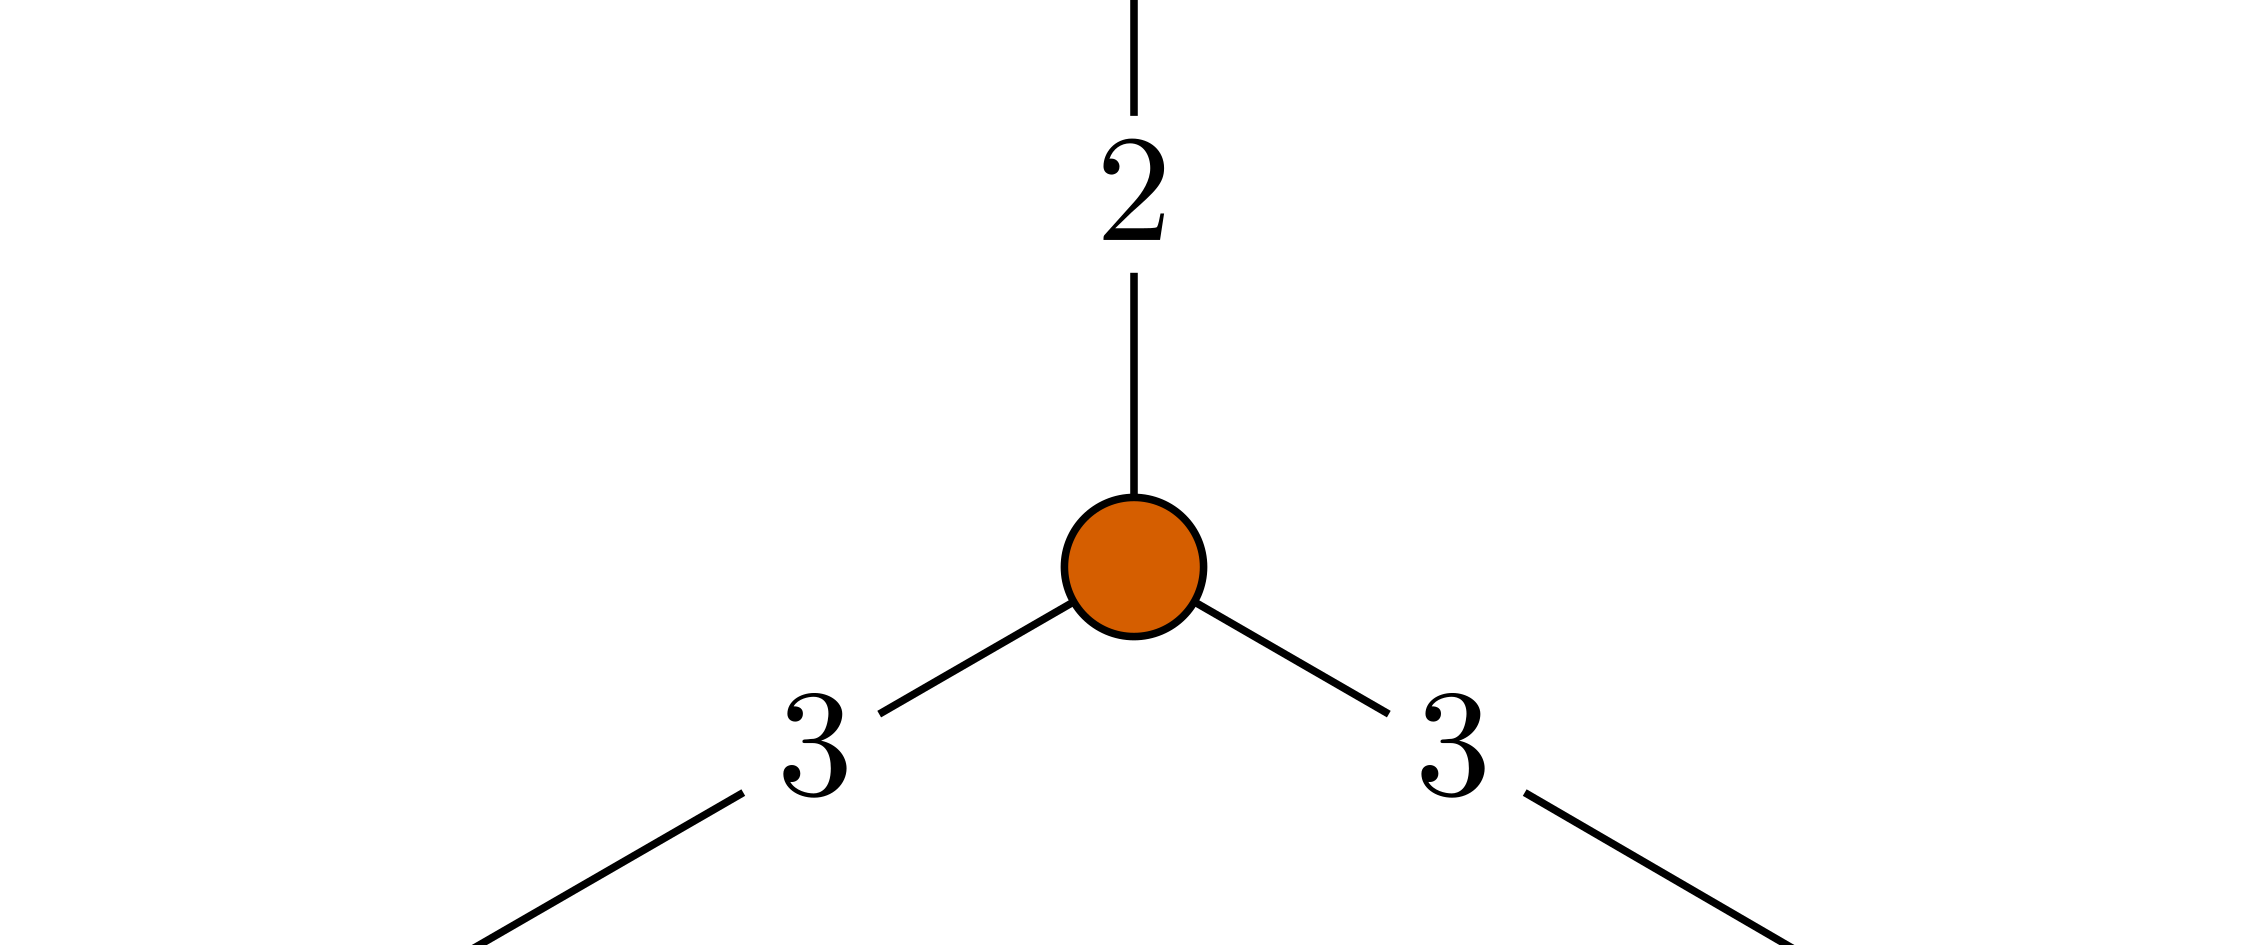
\includegraphics[width=\textwidth]{Figure 15.3.C}
\caption{This trigram obeys both triangle inequality and fermion conservation}
\end{figure}
\noindent
A fermion is an odd particle and a boson is an even particle, therefore any odd-valued trigram sums in the spin network would result in the fermionic particle becoming a bosonic particle. This is not how most matter behaves, but there may be some odd cases where it occurs in real-life.

Penrose's original 1971 paper on angular momentum can determine a spin network's value $\alpha$ and norm $\langle \alpha | \alpha \rangle = || \alpha ||^2$ by first forcing a network closed upon itself (if it is open):
\begin{figure}[H]
\centering
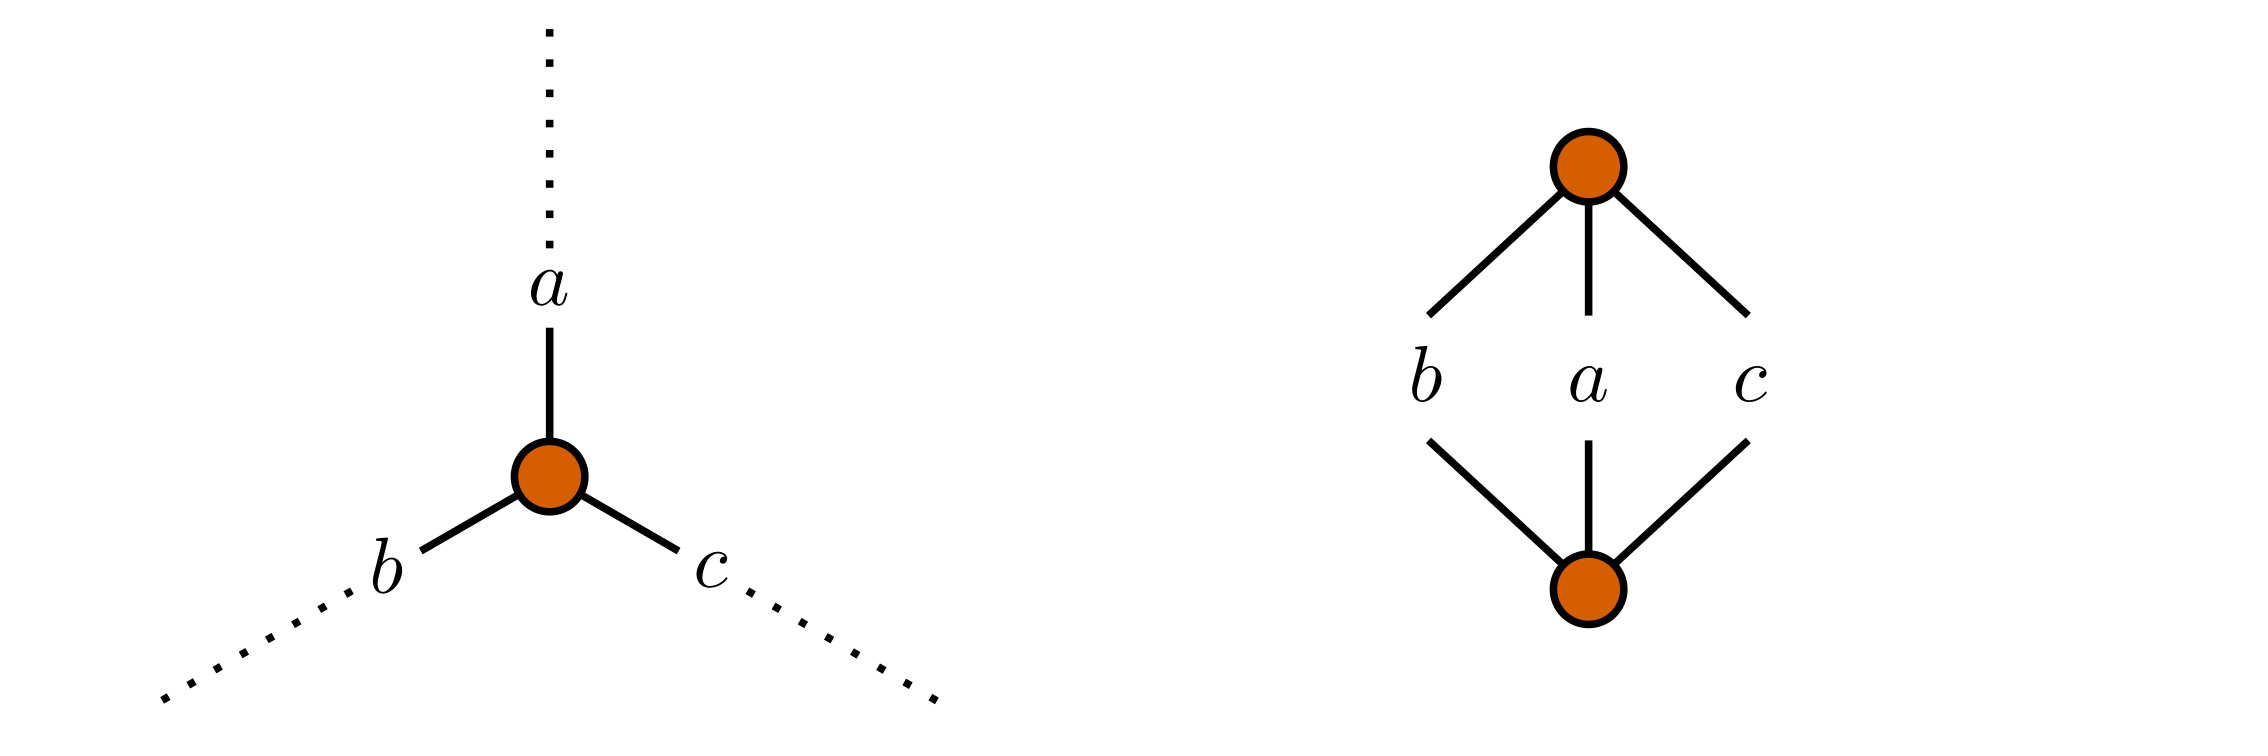
\includegraphics[width=\textwidth]{Figure 15.3.D}
\caption{Closing an open spin network}
\end{figure}
\noindent % Closing an open spin network
and represent each spin$\times 2$ exchange as a strand of $2 s_P$ wires that may not loop in on itself in the open network form:
\begin{figure}[H]
\centering
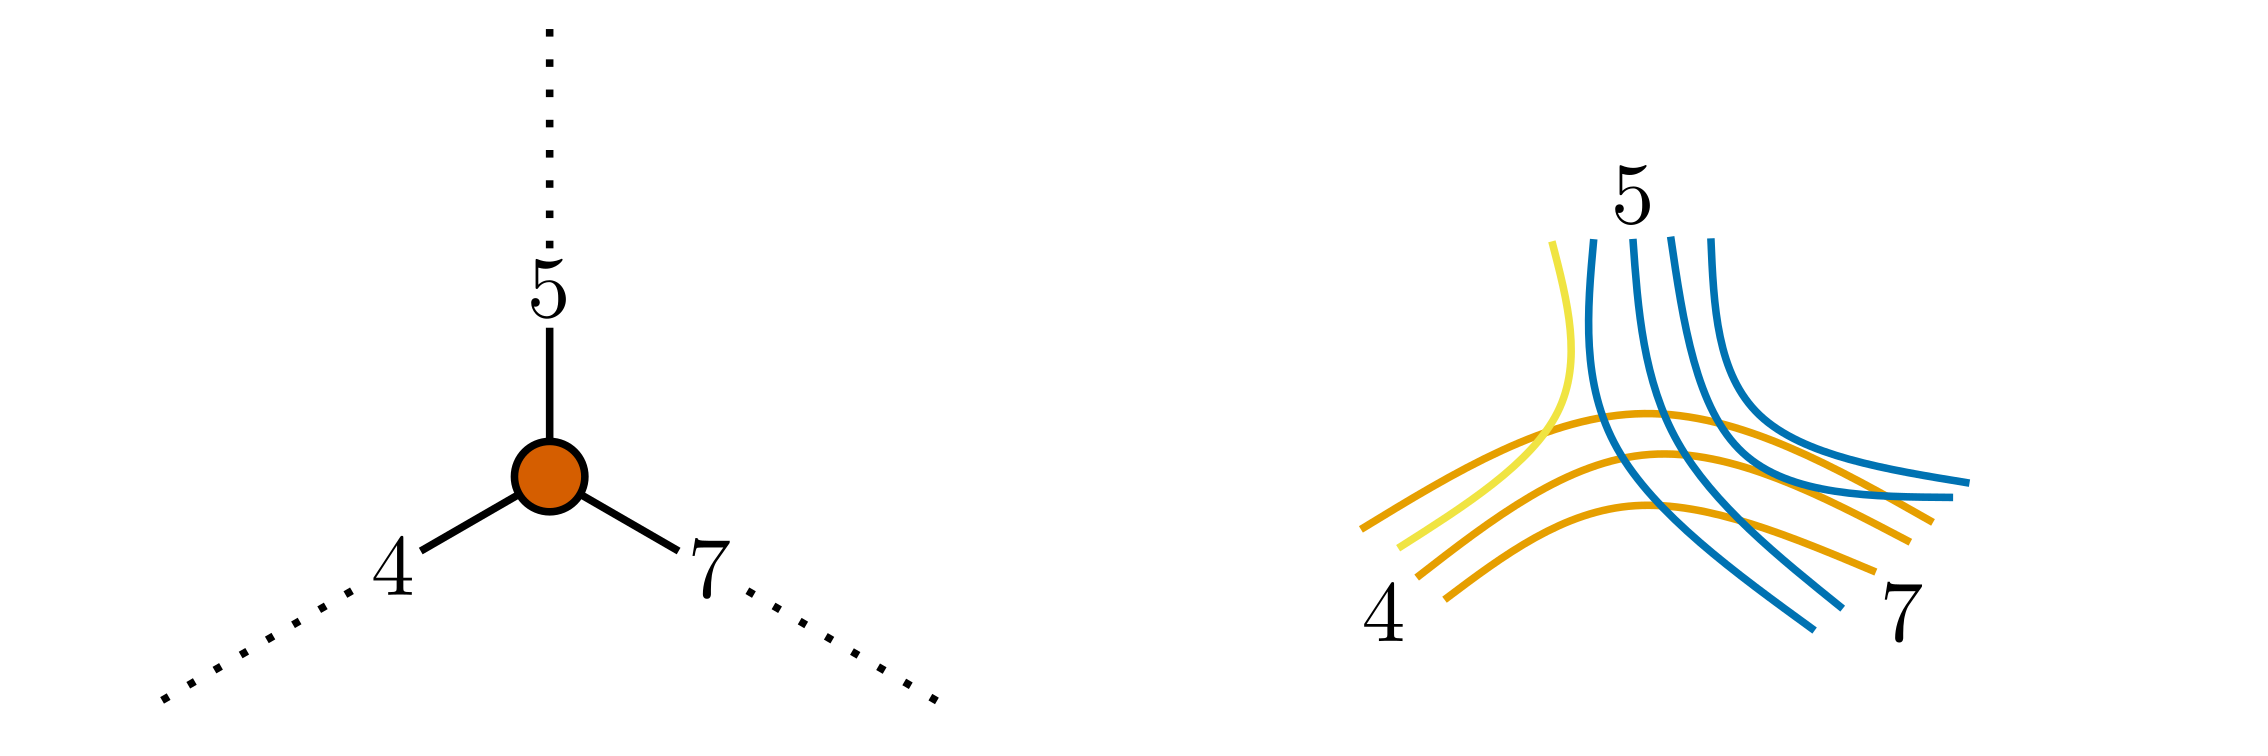
\includegraphics[width=\textwidth]{Figure 15.3.E}
\caption{Conversion of a spin network into a loop network, not allowing strings to self-loop}
\end{figure}
\noindent % Converting a spin network to a loop network
This converts a spin network representation to the loop network representation.

Boolean random walks, as a type of $\operatorname{U}(1)$ lattice gauge theory, would mutually benefit from the study of lattice gauge theory for electromagnetism. Generalizations of Boolean random walks would in turn advance the study of spin networks and loop quantum gravity. Since loop quantum gravity directly depends on the study of spin networks and spin foams, the study of Boolean random walks and models of electromagnetism inside of it would benefit the advancement of fundamental physics. 


\section{Constructor Theory}
\textbf{Constructor theory}\index{constructor theory} is not an exact model of fundamental physics per se. It is a more general theory of allowed information processes, a claim that the laws of physics are derived from basic laws regarding information. A physical process may be carried out if and only if a constructor that generates it may exist. These constructors may be combined in order to produce a computation medium. By iteratively applying an instruction or a set of instructions, a constructor en masse will arrange itself into a permutation as governed by those instructions.

Constructors do not rely on a specific information basis, or rather information does not rely on a specific constructor. It is the method by which fluids locally transfer pressure that allows for liquids and gases to propagate longitudinal waves, alternatively called pressure waves or compression waves. As long as some measure is preserved globally in a closed system and the constructor transforms its value locally, then the computation medium should tend towards information states that locally minimize the potential energy according to the constructor's instructions.

In terms of Boolean statistical mechanics, a Boolean constructor is simple: Iteratively apply a set of rules that preserves the constructor. The complex answer is that a constructor should iteratively apply a set of rules that maximizes preservation of the constructor. Physics would need more than constructors that only preserve themselves. Real physical processes often contain temporary or impermanent information states, thus requiring temporary or impermanent constructors. A photon naively obeys its instructions, randomly absorbed and ejected until its energy is entirely bound to create a new particle or it is bound as momentum to an existing particle.

\section{String Theory and Theories of Everything}

The ultimate goal of physics is develop a \index{theory of everything}\textbf{theory of everything} to describe every possible interaction in the universe. That ideal is hard to achieve. It requires creating a leap in logic so fundamentally radical that no proof can be made of its validity before it is funded. A risk that no granting agency will take until the deed is already done. A less risky step is to invest in uniting the two most important theories of physics, a safe and wise yet foolish and unlikely endeavor.

\textbf{String theory}\index{string theory} and its variants are some of the oldest theories put forth to unite the Standard Model of quantum mechanics' discreteness against General Relativity's continuous deformation of spacetime. The controversy of string theory is not simply its perceived failure, but its monopoly on financial and intellectual resources since its introduction. Unfortunately, young scientists in physics are forced to match the research preferences of their senior established researchers. This is true of any scientific discipline, but it prevents truly original research from emerging if interests do not match. This was not a problem New College of Florida because it took a student-centered approach to undergraduate education. Student-centered approaches to education should not occur at the graduate level, the undergraduate level, nor the secondary level. The first country to do so at the primary level wins the race.

As I understand it, straying from the crowd is career suicide. This not merely a physics community problem but a homo sapiens problem. The failure of modern academia is investment in measurable results instead of investment in individuals. That does not mean naively giving money to individuals lacking integrity, talent, or motivation. It is about changing the perspective of how scientific knowledge is created: in the mind of an individual observing the world. Trailblazers will always exist, but will they have the grace of a shovel or must they dig with their bare hands?

As things stand, an idea such as Boolean statistical mechanics would have been killed in its infancy at a so called prestigious academic institution. Not because the idea itself is not worth researching but because the idea will not advance my career prospects. The incremental progress of science via low-hanging fruit that produces measurable results is limited by our ability to identify results worth measuring. All of the things we appreciate now are the result of bright individuals driven by a passion for knowledge putting forth their best effort during their younger years.




\appendix

\chapter{Eigenclass Formalization}
The definition of \textbf{eigenclass}\index{eigenclass} that we use throughout the textbook was an inexact concept long after the first draft. After some deeper consideration of the problem and discussions with colleagues, I propose the following thought experiments to assist us in creating a suitable definition.

Consider the following potential function of a particle traveling in a $1$-dimensional chamber. Each potential well is defined by a Gaussian function:
\begin{figure}[H]
\centering
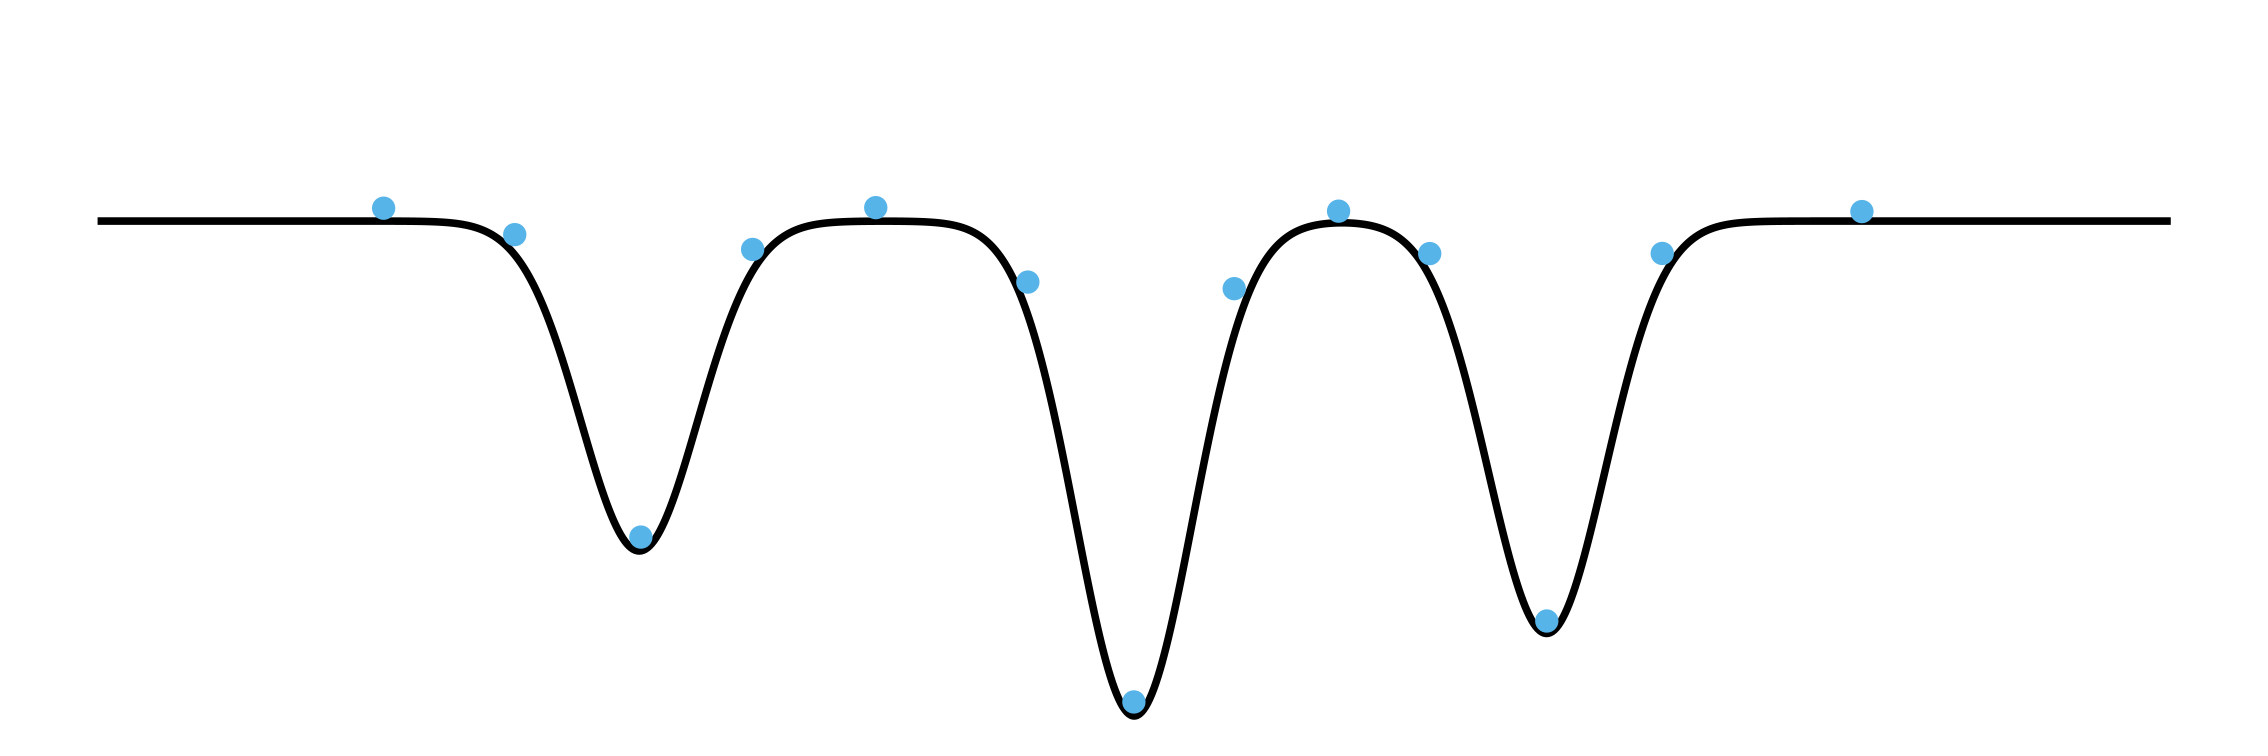
\includegraphics[width=\textwidth]{Figure 16.1.A}
\caption{A potential function with 3 minima that may be found by derivatives via an optimizer}
\end{figure}
\noindent % A potential function with 3 potential minima in 1D
It is easier for the particle to crawl down a potential well than up, but it is still possible. There are three potential minima that a particle can tend towards, and we can determine this using the second derivative. Any optimizer will find any of the three minima without issue.

Consider a similar potential function in which we replace each Gaussian function with a sombrero function. There are still three major potential wells, but there are many minor potential wells surrounding them due to the bumpiness of a sinc function:
\begin{figure}[H]
\centering
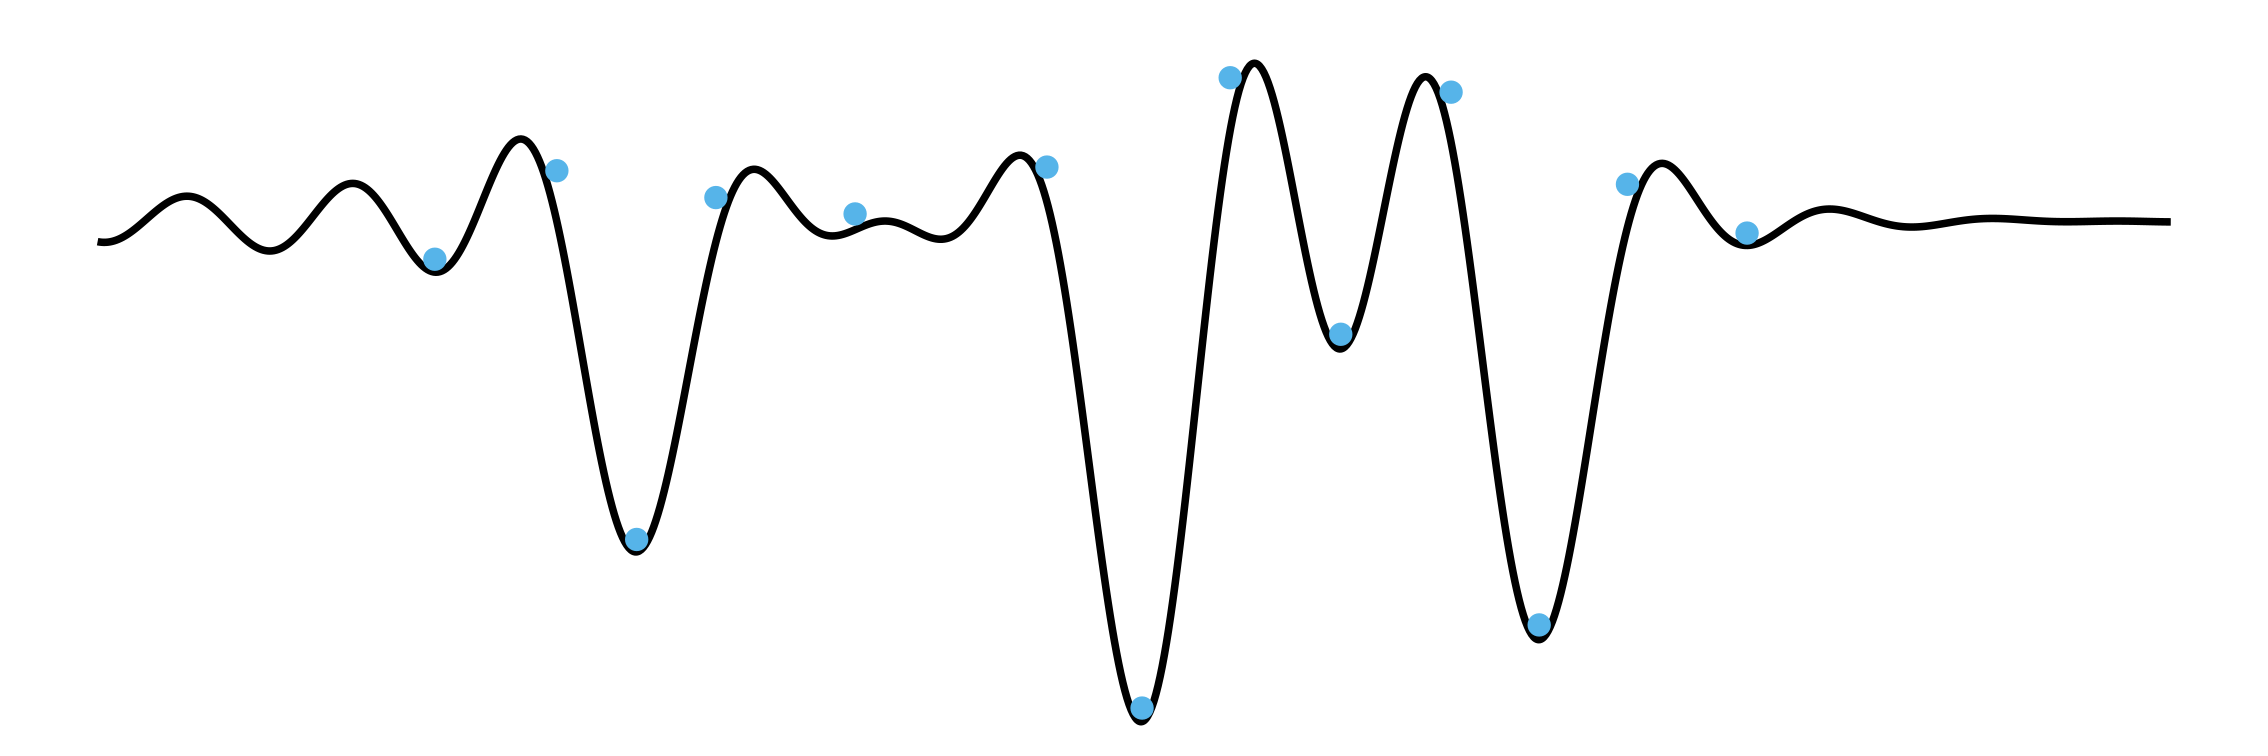
\includegraphics[width=\textwidth]{Figure 16.1.B}
\caption{The same potential function with various high frequency bumps}
\end{figure}
\noindent % A potential function with 3 obvious potential minima in 1D, but the sinc function makes it bumpy
The major potential minima are obvious to a human eye but not obvious to an optimization algorithm. We cannot rely on a second derivative optimizer because it may be trapped in a nearby local minima. 

If we were to rely on Fourier analysis, we could remove the high frequencies from the minima due to their slow decay in the heat equation. We can easily declare the most important minima using our eyes, but that is dependent upon our subjective cognition. More importantly, the strategy does not scale to higher dimensions or discrete optimization problems. Is there a mathematical way to amend these problems?

Consider the following model of gas particles in a 2D chamber, mimicking five chemistry flasks connected together:
\begin{figure}[H]
\centering
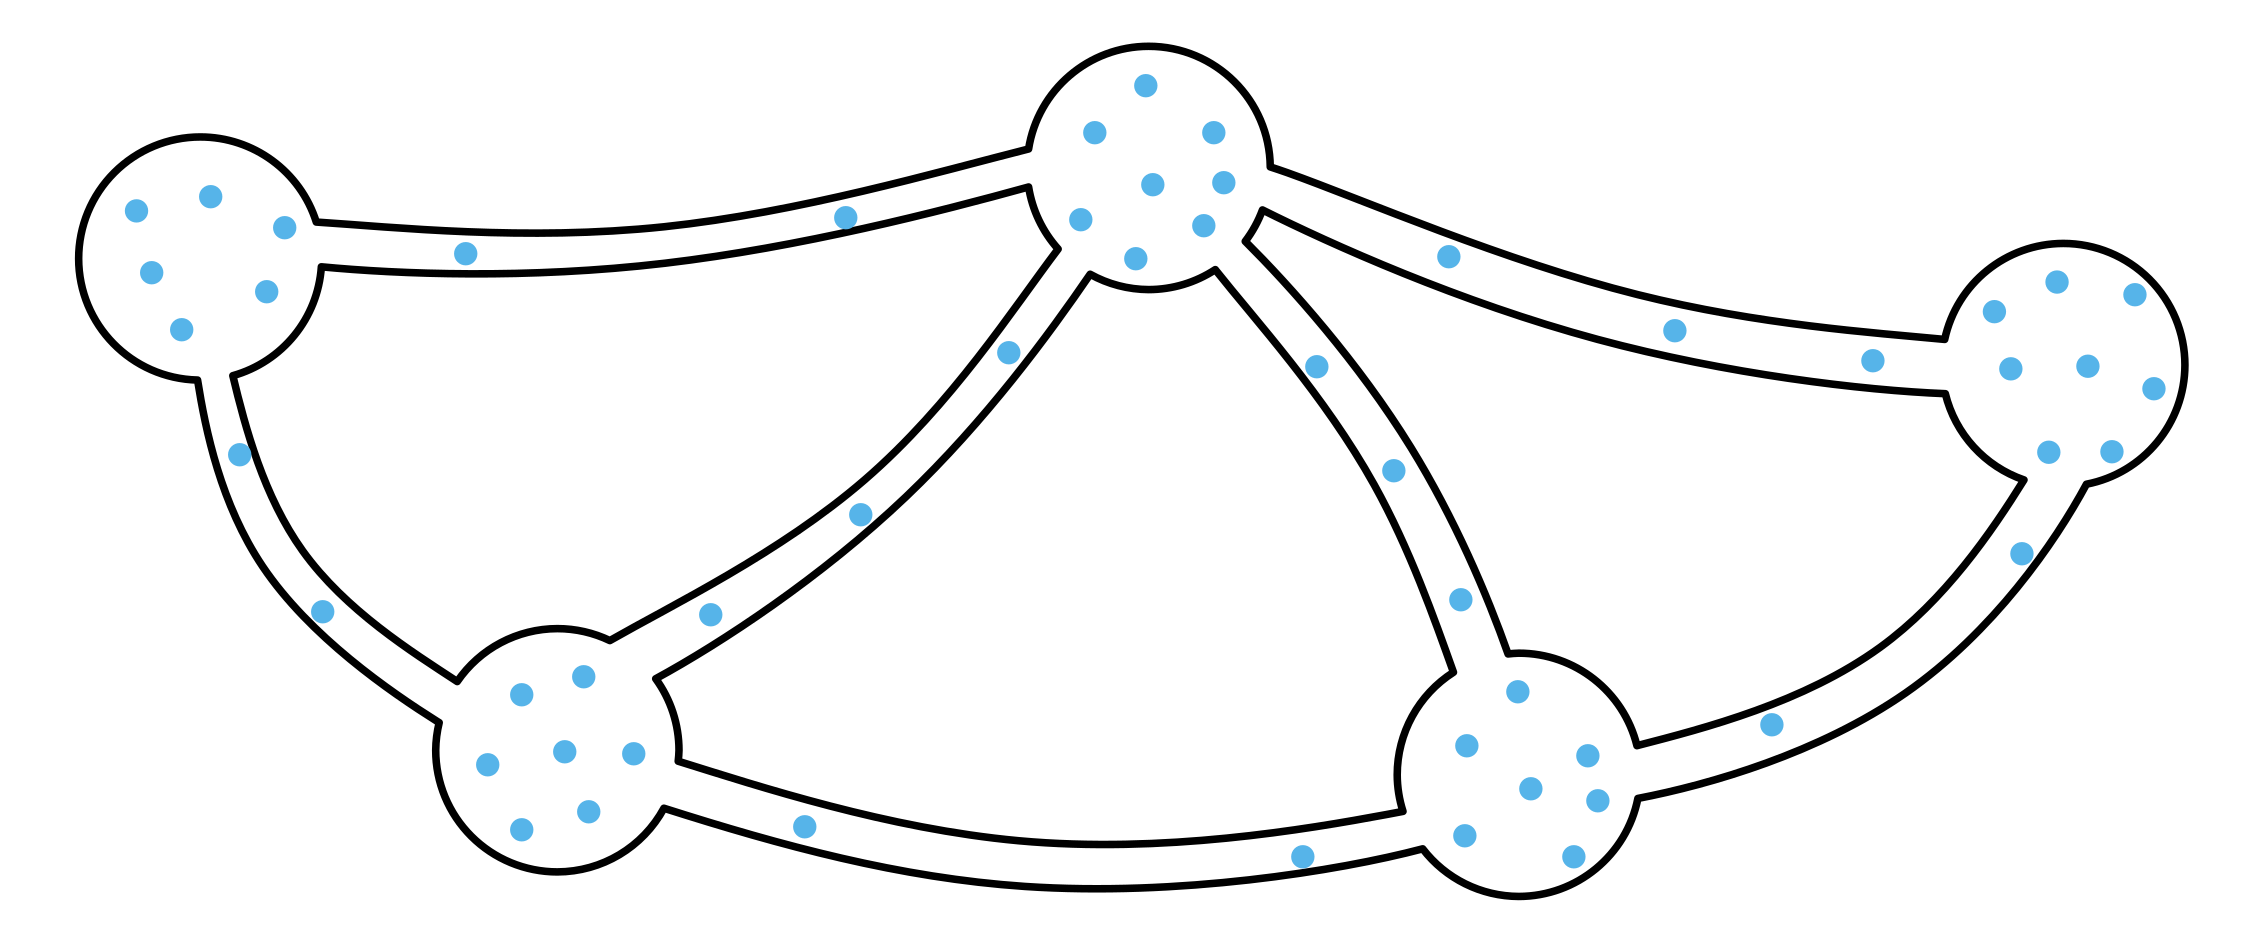
\includegraphics[width=\textwidth]{Figure 16.1.C}
\caption{A representation of 5 gas chambers in 2D}
\end{figure}
\noindent % A series of 5 gas chambers in 2D
The gas particles flow freely within each flask and along tubes, but they may not pass through the glass walls. From the perspective of a lone gas particle, how do we know that there are precisely $5$ chambers? How does our human vision system designate that there are $5$ countable chambers?

How does this relate to Boolean statistical mechanics and eigenclasses? When we are looking at a communication class in a Markov chain, we are interested in how many states can reach each other. As time passes, all states within a communication class have diffused across the entire communication class.\footnote{Except for the odd case of periodic Markov chains, in which case the initial states may be separated by phase in a cycle.} They reach a stationary distribution, and all initial distributions in that communication class point in the one direction. Before they all become one, all states are orthogonal at time $t=0$ as represented by the stochastic matrix $P^0 = I$.

Define $\Theta(t)$ to be some matrix such that $\Theta_{(i,j)}$ represents the correlation or cosine similarity between row $i$ and row $j$ of the stochastic matrix $P^t$:
$$\Theta_{(i,j)}(t) = \frac{ P^t_{(i, \cdot)} \cdot P^t_{(j, \cdot)} }{ ||P^t_{(i, \cdot)}|| ||P^t_{(j, \cdot)} ||}$$
At time $t=0$, the correlation value for non-diagonal entries is $0$ for all stochastic matrices. As time $t \rightarrow \infty$, the correlation between each state is $1$ within an ergodic communication class. Thus we define $\Theta(t)$ for all times values $t \in \mathbb N$.

Let us define $k(t)$ to be the sum of all values in the matrix $\Theta(t)$:
$$k(t) = \frac{n^2}{\sum \Theta(t)}$$
Since $P$ is some $n \times n$ matrix, $k(0)$ is always $n$ since any state is correlated with itself and $k(\infty)$ has a minimum value of $1$ for most stochastic matrices. We define $k(t)$ as the \textbf{pseudo-rank}\index{pseudo-rank} of the correlation matrix of stochastic matrix $P$ at time $t$. 

The stochastic matrix at time $t=0$ is the identity matrix $P^0 = I$. The state space of $P^t$ is defined by some $(n-1)$-simplex surface, and each row must be a point on the simplex. As $t \rightarrow \infty$, the estimated number of dimensions compresses towards $1$ if the stochastic matrix diffuses across all states. Somehow, the estimated number of dimensions compresses from $n$ to $1$ due to the fact that the eigenvalues of a stochastic matrix are bounded by $|\lambda| \leq 1$.

We also define $m=\lceil k(t) \rceil$ to be the minimum number of rows and columns needed to sufficiently represent $P^t$ as a lower-order matrix $Q$:
$$P_{n \times n}^t \approx Q_{m \times m}, \quad m = \lceil k(t) \rceil, \ m << n$$
The order of matrix $P^t$ is approximately $m$. At the limit of infinite time steps, the value for $\lceil k(\infty) \rceil$ equal to the number of recurrent classes times the period of each class.\footnote{If $d_i$ is the period of class $i$, then $\lceil k(\infty) \rceil = \sum d_i$ is the number of unique limiting distributions.}

If we think of the cyclical stochastic matrix with two different communication classes:
\[P = 
\left[ \begin{array}{c c|c c c}
0 & 1 & 0 & 0 & 0 \\
1 & 0 & 0 & 0 & 0 \\
\hline
0 & 0 & 0 & 1 & 0 \\
0 & 0 & 0 & 0 & 1 \\
0 & 0 & 1 & 0 & 0
\end{array} \right]
\]
then $\lceil k(t) \rceil \rightarrow \frac{25}{2+3}$ as $t \rightarrow \infty$. The estimated number of classes is exactly $5$, therefore we need $Q$ to be a rank $5$ matrix to sufficiently approximate $P^{\infty}$.

If we think of a matrix that will perfectly diffuse but has two communication classes:
\[P = 
\left[ \begin{array}{c c|c c c}
\frac{1}{2} & \frac{1}{2} & 0 & 0 & 0 \\[2pt]
\frac{1}{2} & \frac{1}{2} & 0 & 0 & 0 \\[2pt]
\hline \\[-2.3ex]
0 & 0 & \frac{1}{3} & \frac{1}{3} & \frac{1}{3} \\[2pt]
0 & 0 & \frac{1}{3} & \frac{1}{3} & \frac{1}{3} \\[2pt]
0 & 0 & \frac{1}{3} & \frac{1}{3} & \frac{1}{3}
\end{array} \right]
\]
then have $\lceil k(t) \rceil \rightarrow \lceil \frac{25}{4+9} \rceil$ as $t \rightarrow \infty$. The estimated number of classes is approximately $1.923$, we need $Q$ to be at least a rank $2$ matrix to sufficiently approximate $P^\infty$.

The value that this provides to Boolean statistical mechanics is that the number of potential wells for a stochastic matrix $P$ is much less obvious than a potential function. We cannot rely on the derivative of $k(t)$ to determine an optimal number of classes because $\frac{d}{dt} k(t)$ relates to the eigenvalues $\lambda_1,...,\lambda_\theta$ of $P$. Since each $\lambda^t$ is an exponential function of $C^\omega$ analytic smoothness, the sum of correlations $k(t)$ is likewise a $C^\omega$ smooth functions. This means we should rely on the elbow method to define the number of classes, such as if we use the $k$-means clustering algorithm.\footnote{The elbow method in cluster analysis is often decried as dependent upon human subjectivity. Now we have an analytic reason of why derivatives do not work in cluster analysis.}

As initial states in stochastic matrix $P^t$ become more correlated, initial states with similar future distributions merge. We might think of eigenclasses as a vertical slice of some tree diagram as time progresses:
\begin{figure}[H]
\centering
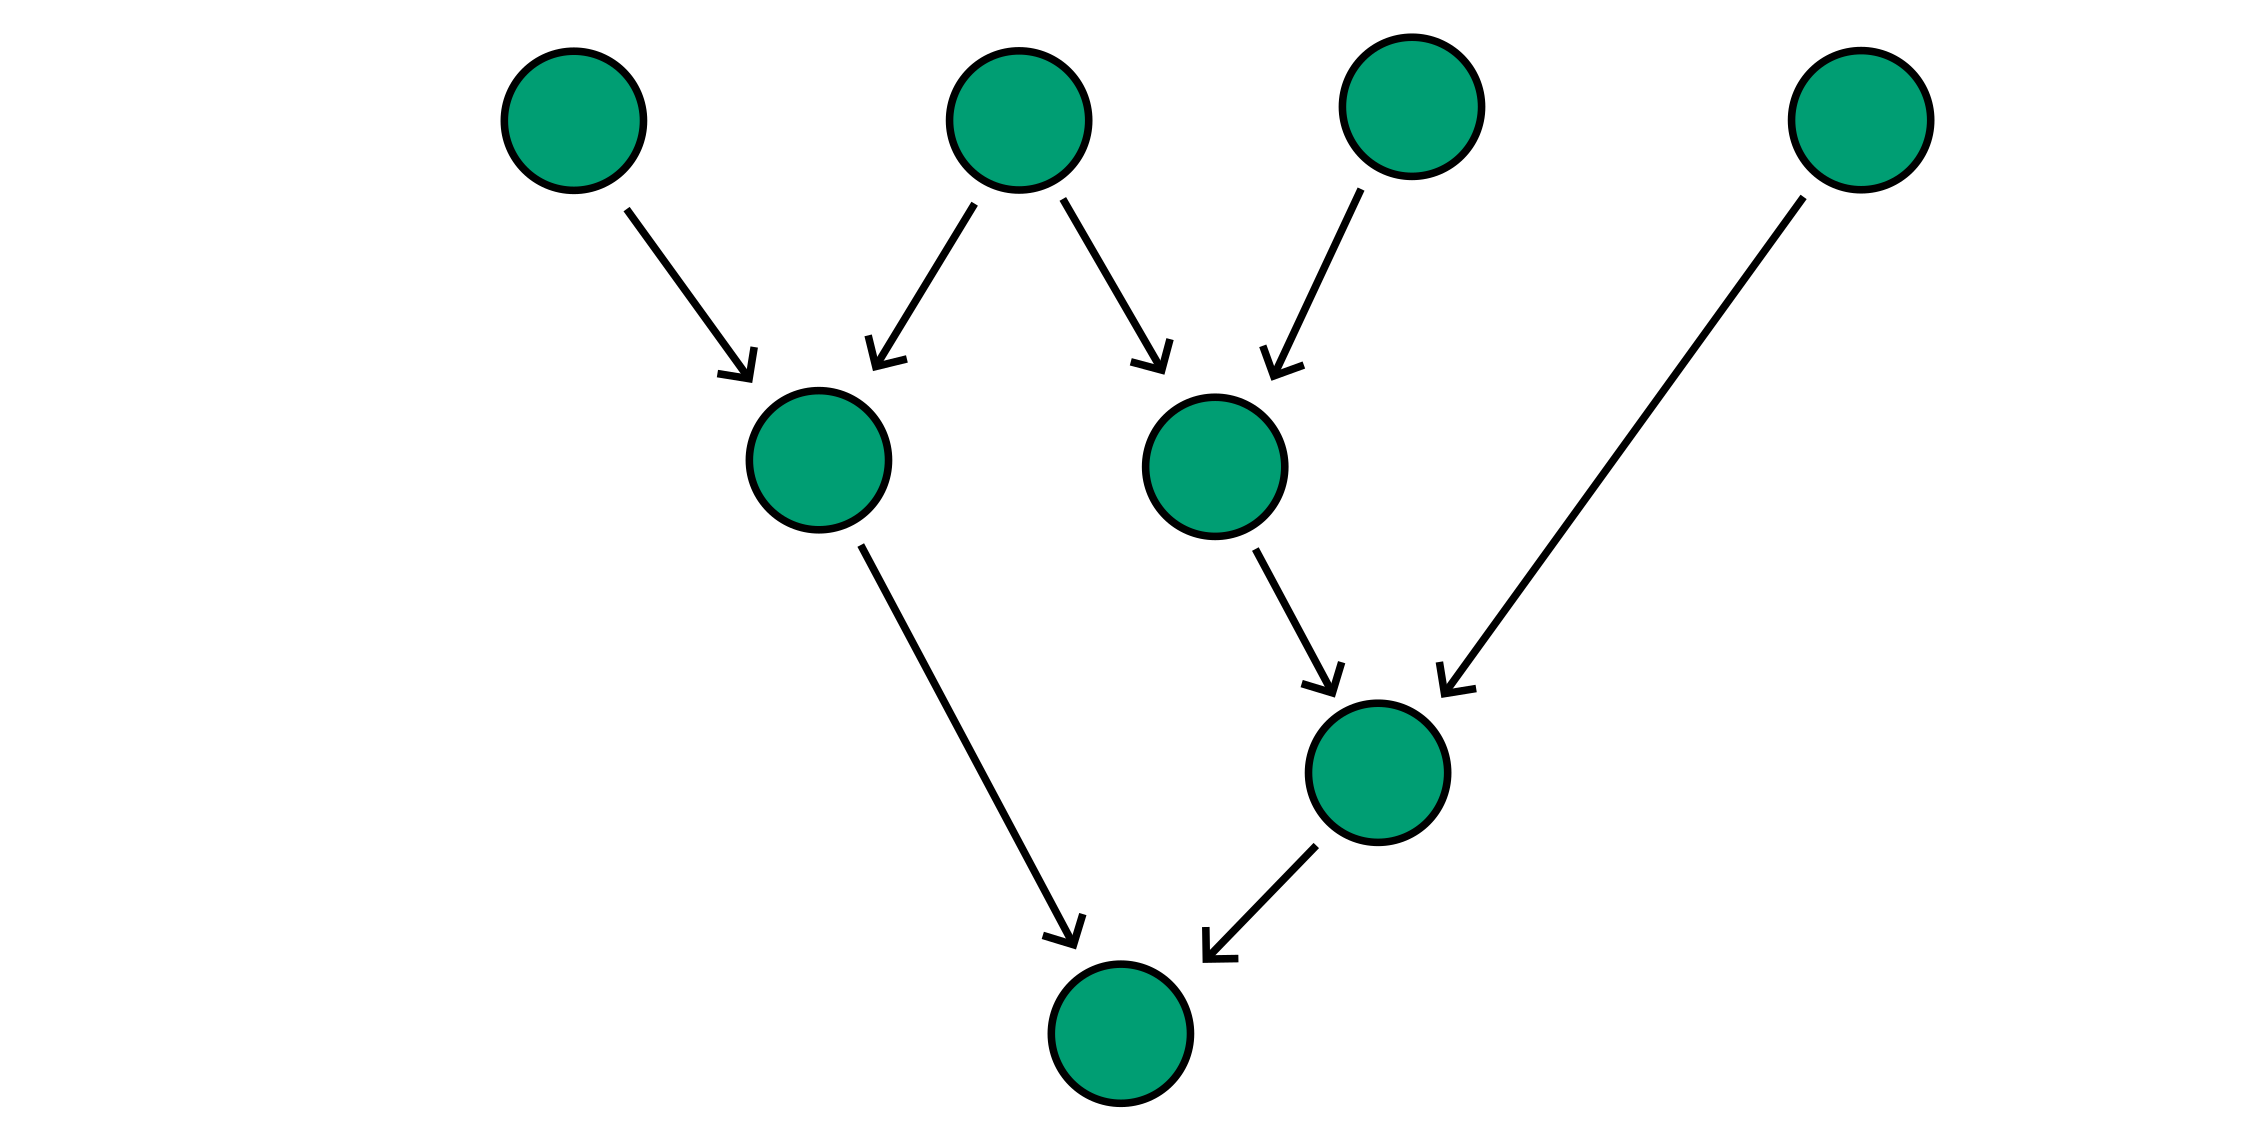
\includegraphics[width=\textwidth]{Figure 16.1.D}
\caption{The merging of initial distributions with similar future distributions form a taxonomic class or category}
\end{figure}
\noindent
Suppose that we do a discrete approximation of the gas chambers example. If we use the elbow method to stop at $\lceil k(t) \rceil = 5$ classes the optimal classification of initial points looks something like this:
\begin{figure}[H]
\centering
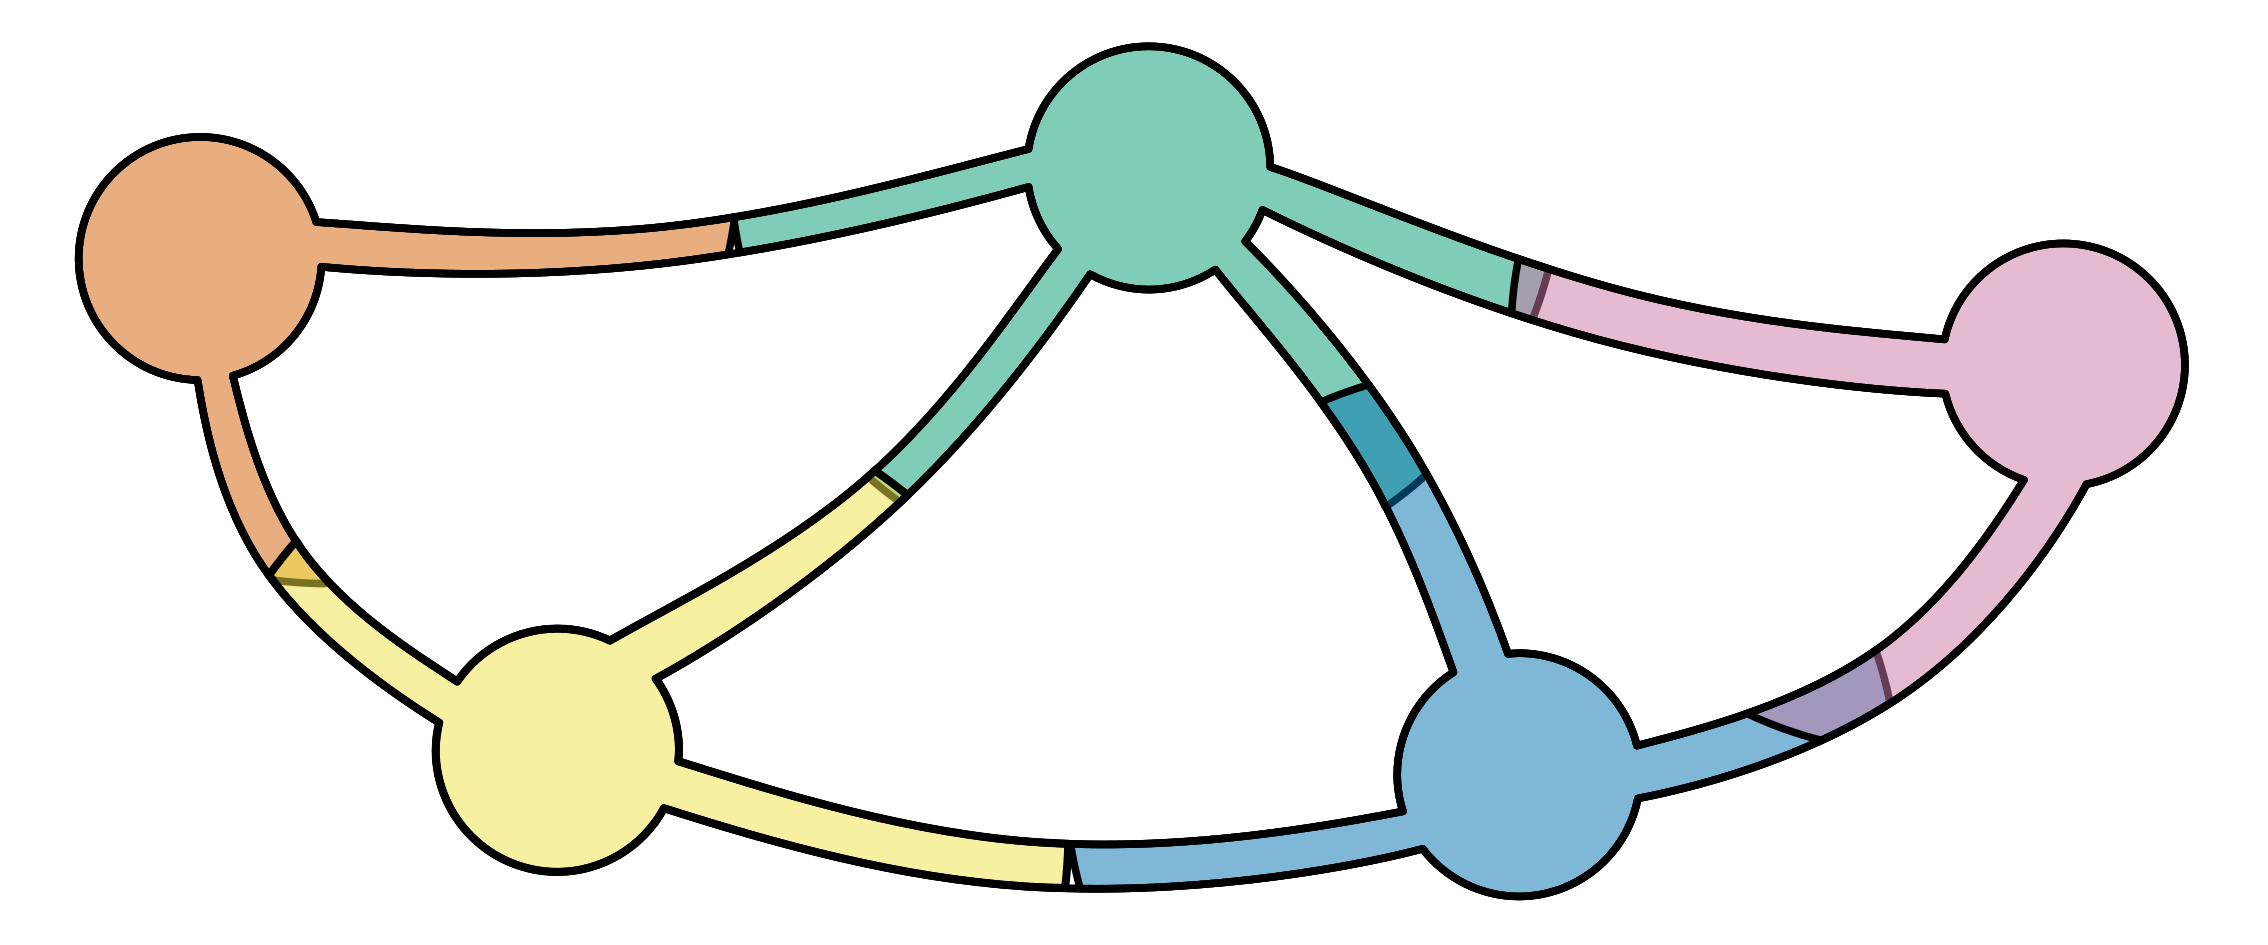
\includegraphics[width=\textwidth]{Figure 16.1.E}
\caption{The five classes of a gas chamber are due to ``bottlenecks'' that restrict flow}
\end{figure}
\noindent % Image of five gas chambers connected by thin tubes
The probability distribution of a single gas particle will easily spread within its chamber, but how quickly it spreads will \textit{bottleneck} due to the thin tubes connecting the gas chambers. We might think of it as a sharp decrease in the rate of unions, fusions, or anti-bifurcations occurring in the stochastic matrix.

One possible method for determining a temporal class is \textbf{$\boldsymbol{k}$-means clustering}\index{k-means clustering}. A $k$-means clustering algorithm seeks to assign $n$ points to $k$ clusters by minimizing the average distance to a cluster, and this is useful for the context of determining where to assign rows of a stochastic matrix based upon their future distribution:
\begin{figure}[H]
\centering
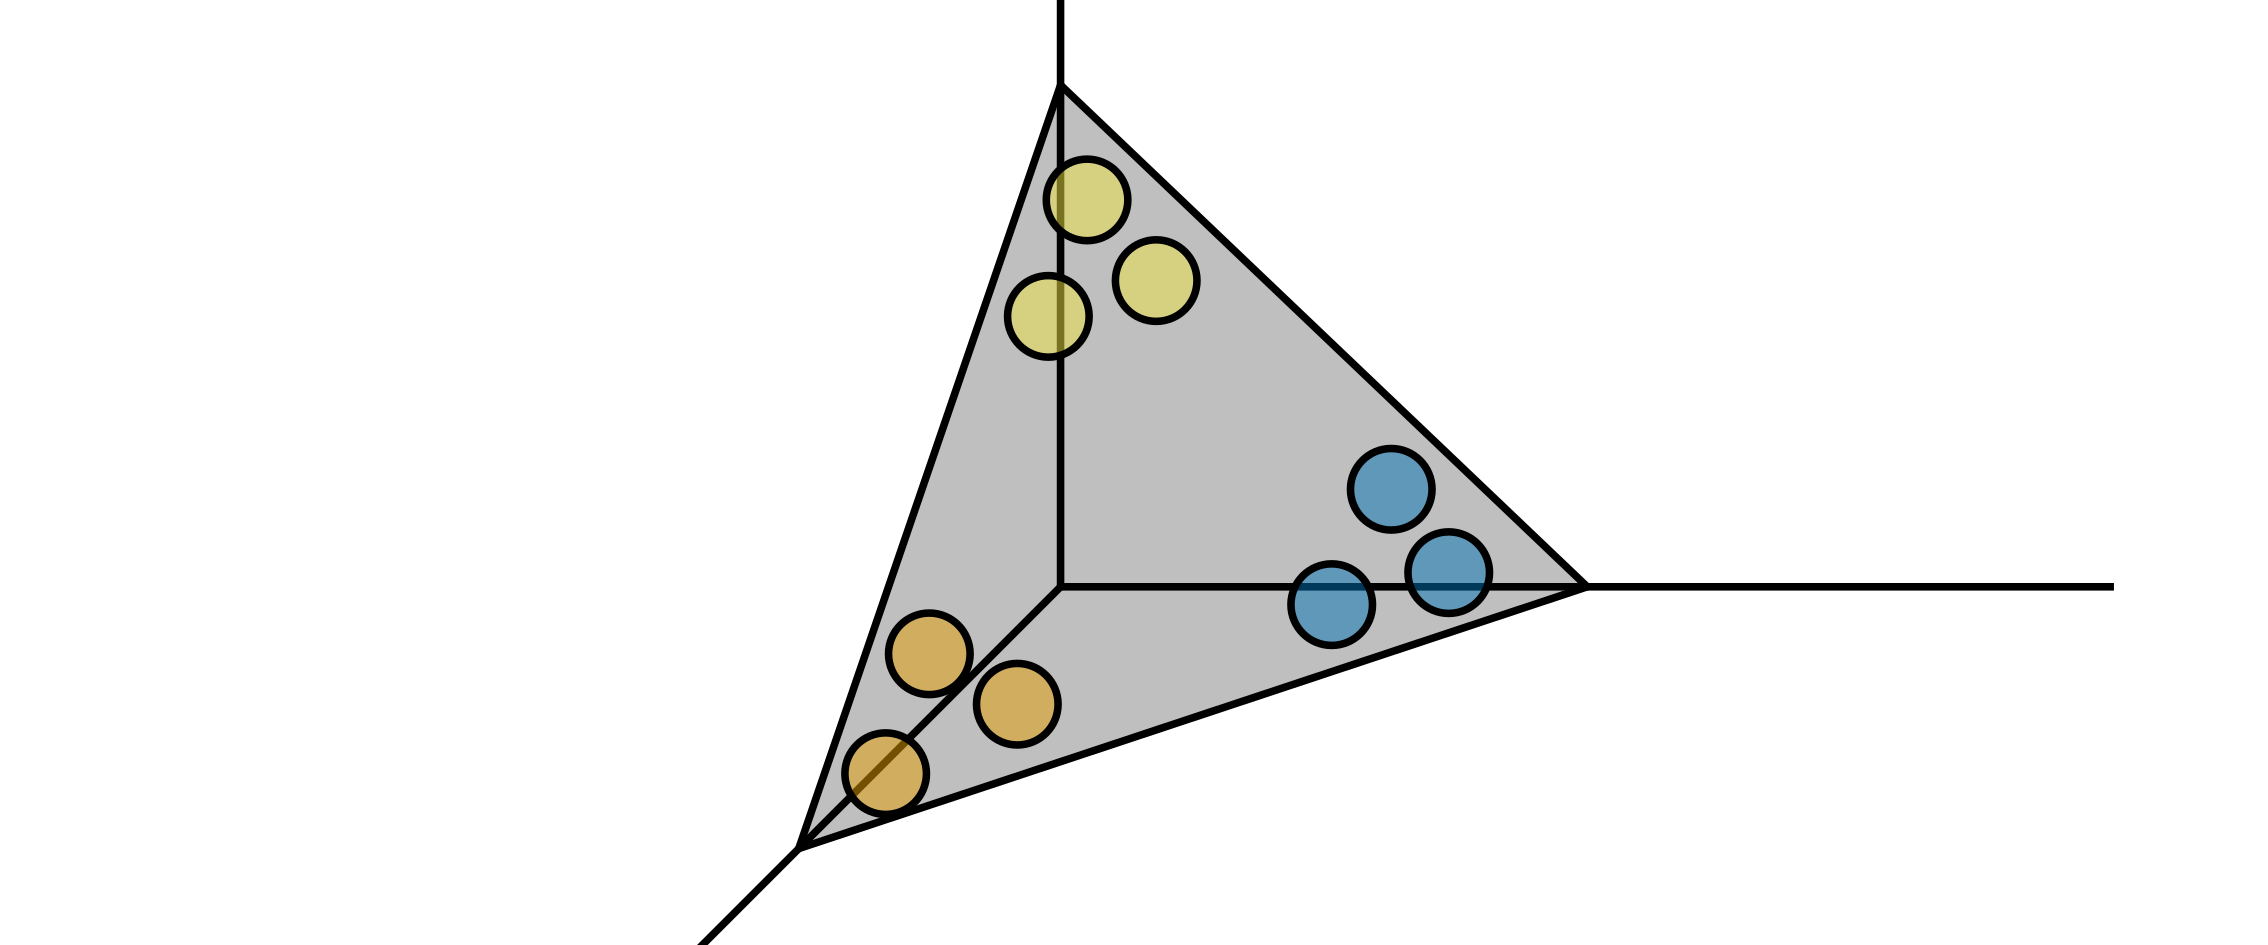
\includegraphics[width=\textwidth]{Figure 16.1.F}
\caption{A $2$-simplex as the projection of $9$ states into $3$ classes due to clustering}
\end{figure}
\noindent % A 2-simplex
In this example, there are approximately $\lceil k(t) \rceil = 3$ possible clusters that a point may be assigned to. 

The flow of these $n$ points must flow upon some $(n-1)$-simplex as governed by the eigenvalues of the stochastic matrix $P^t$. We need at most some $(m-1)$-simplex for our projection into a lower-order matrix, in which $m = \lceil k(t) \rceil$. This is a form of \textbf{dimensionality reduction}\index{dimensionality reduction} for stochastic matrices, at it is based on the idea that the determinant $|P^\infty|=0$. While $k$-means clustering is a decent naive assumption, we need an algorithm that leverages the unique property that a probability distribution for each row of $P^t$ is bound to the $(n-1)$-simplex and may be projected to some $(m-1)$-simplex. \footnote{The triangle inequality for cosine similarity is sometimes used to accelerate $k$-means algorithms.}

\chapter{Approximate Dynamical Systems}\label{appendix:raw}
Dynamical systems are of great interest to many systems we wish to predict such as fluids, neuronal systems, robotic control systems, and videos. Most systems in the real world are governed by non-linear dynamics, but we are interested in linear systems of the form:
$$\frac{d}{dt}f(x) = A f(x)$$
in which $A$ is a matrix. 

Most measure spaces (mass, energy, velocity) will be governed by non-linear dynamics. However, probability measure spaces will \textit{always} be governed by linear dynamics:
$$\mu(t+1) = \Lambda_\sharp \mu(t) = P \mu(t)$$
This means that we should consider approximations of the form:
$$f(t+1) \approx \sigma^{-1} \tilde{P} \sigma f(t)$$
The key assumptions for why this work is that are projecting some measure space into a probability measure space using the function $\sigma$, and we can approximate $P$ with $\tilde{P}$:
$$\sigma f(t) \approx \mu(t), \quad \tilde{P} \approx P$$
The pushforward form of our projection is thus:
$$\sigma f(t+1) \approx \tilde \Lambda_\sharp \sigma f(t) \approx \tilde{P} \sigma f(t)$$

We can approximate any non-linear, non-conservative systems because probability is always conserved. What is necessary to optimally approximate any dynamical system? If a dynamical system has $n$ eigenvalues $\lambda_1,...,\lambda_n$, then using the $m$ largest magnitude eigenvalues $|\lambda_1|,...,|\lambda_m|$ will minimize the accumulation of prediction error for any time-dependent measure.

\chapter{Graph Minor Algorithms}
\textbf{Edge contraction}\index{edge contraction} is a way that we may represent collections of states (or macrostates). By merging two vertices $u, v$ connected by an edge, a contracted vertex $w$ is formed containing all edges from both of the original vertices (u, v). \textbf{Graph minors}\index{graph minor} are graphs formed by deleting edges, deleting vertices, and contracting edges:
\begin{figure}[H]
\centering
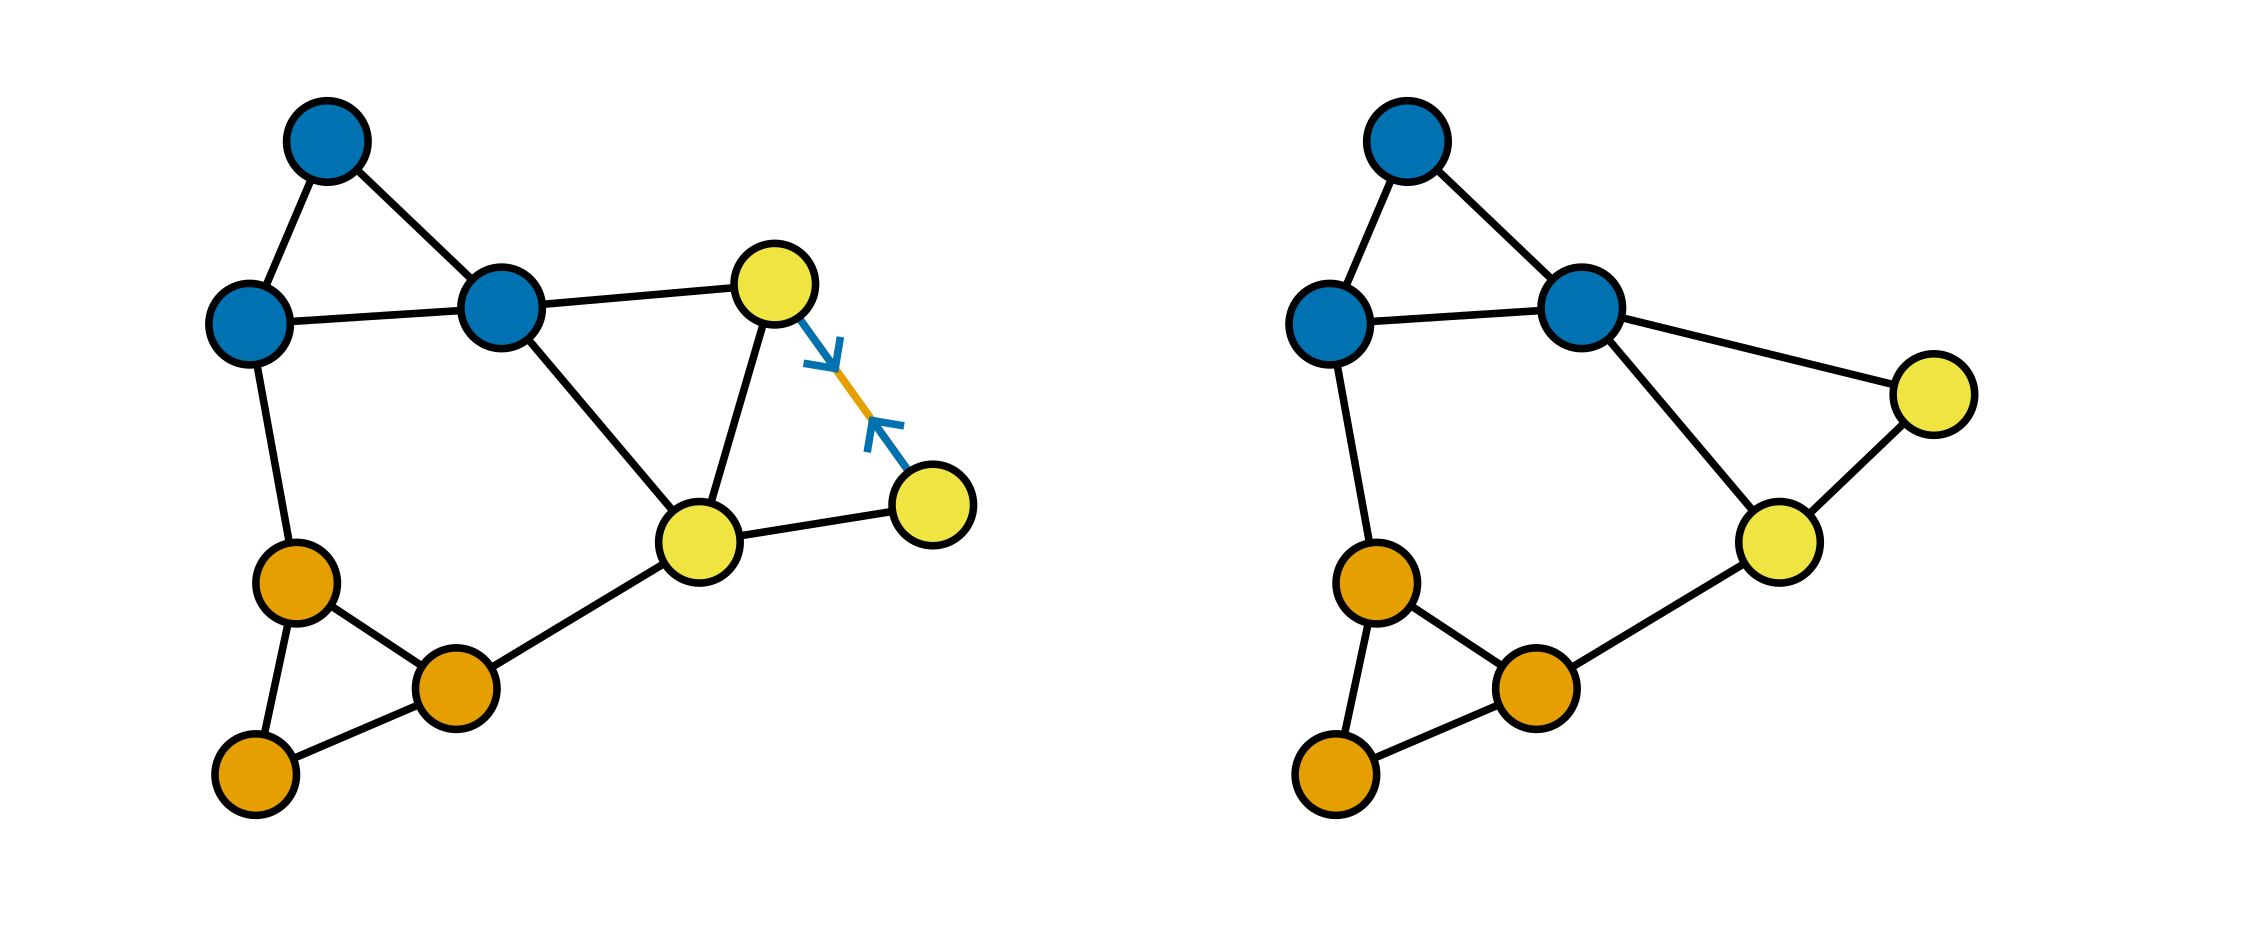
\includegraphics[width=\textwidth]{Figure 16.3.A}
\caption{A graph and its graph minor via edge contraction}
\end{figure}
\noindent % An example of a graph and its graph minor
The graph minor $g$ of the graph $G$ represents a reduced set of information about the original graph. 

Classes define states that strongly communicate with each other. When states in a Markov chain cluster on a simplex due to similar futures, we contract their edges in the state space $\mathcal X$ to form a macrostate. Each macrostate defines a corner of a reduced dimension simplex. What does that mean? What about graphs not representing Markov chains? Without some way to measure some value of a graph and its minor graph, there is no objectivity in determining how to contract edges.

Assume that every graph is a directed graph with self-loops and may represent a Markov chain:
\begin{figure}[H]
\centering
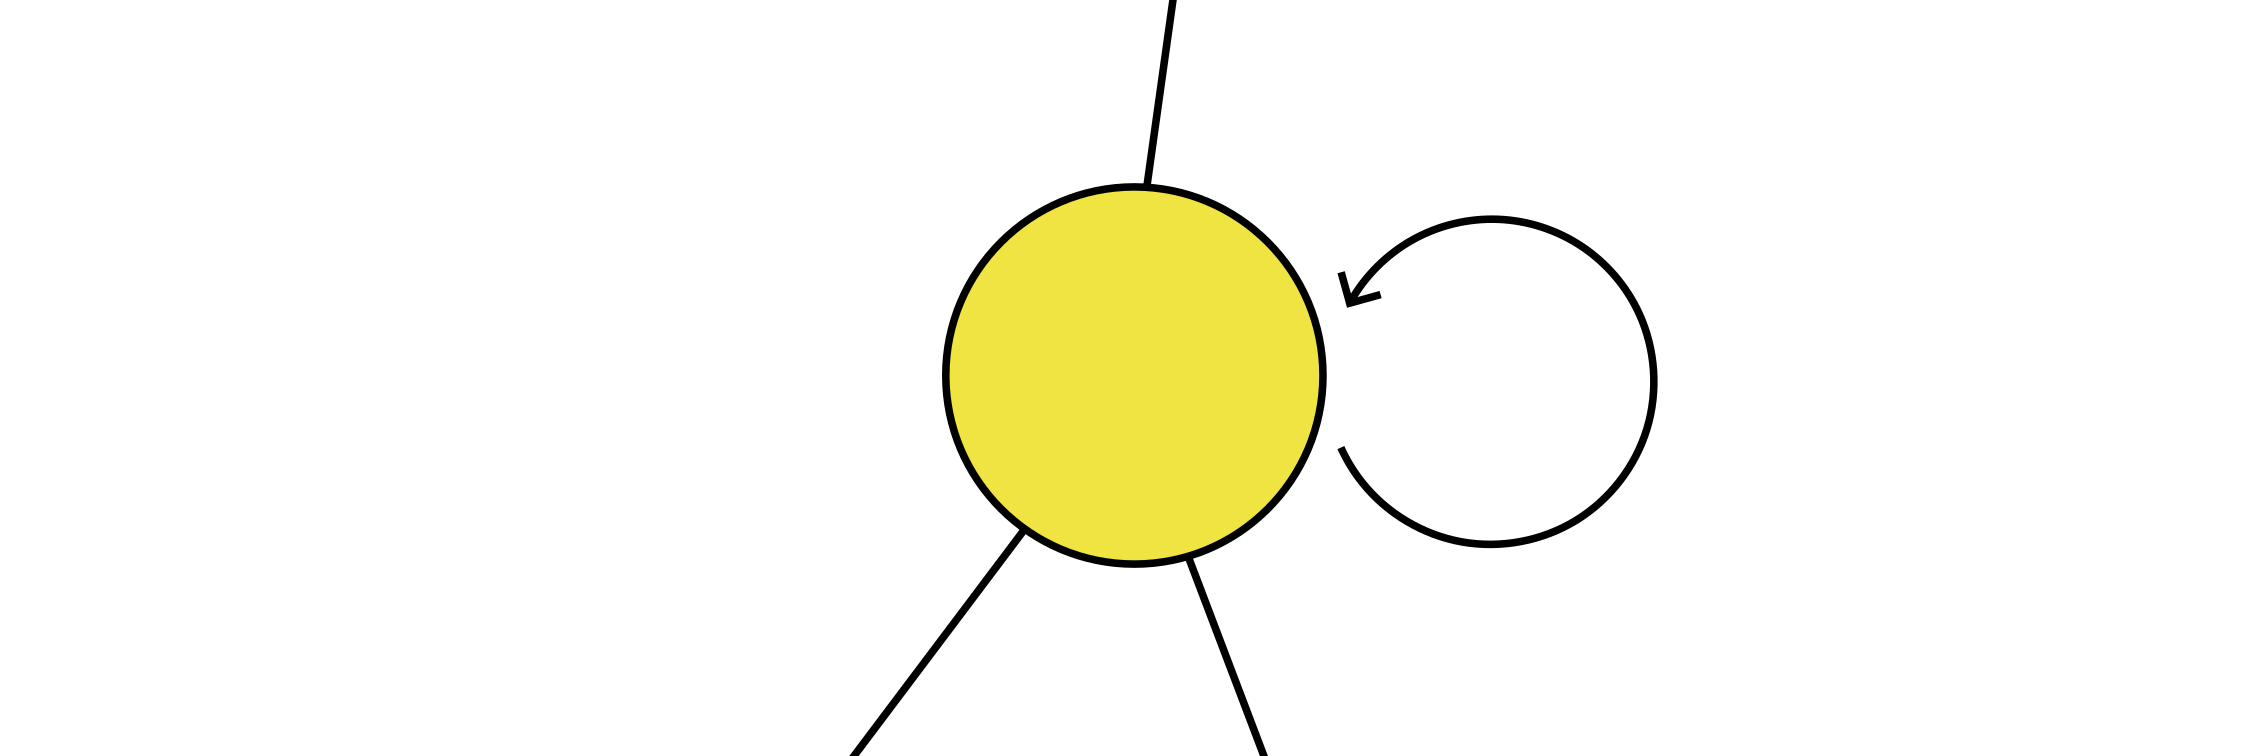
\includegraphics[width=\textwidth]{Figure 16.3.B}
\caption{A directed graph with self-loops is a necessary assumption for merging via aperiodic Markov chains}
\end{figure}
\noindent % A directed graph with self-loops
We claim that edges of a graph should contract to merge vertices if and only if they communicate strongly. We create the assumption that every graph is a stochastic matrix for an aperiodic Markov chain.

Observe the following example of some graph representing $5$ states:
\begin{figure}[H]
\centering
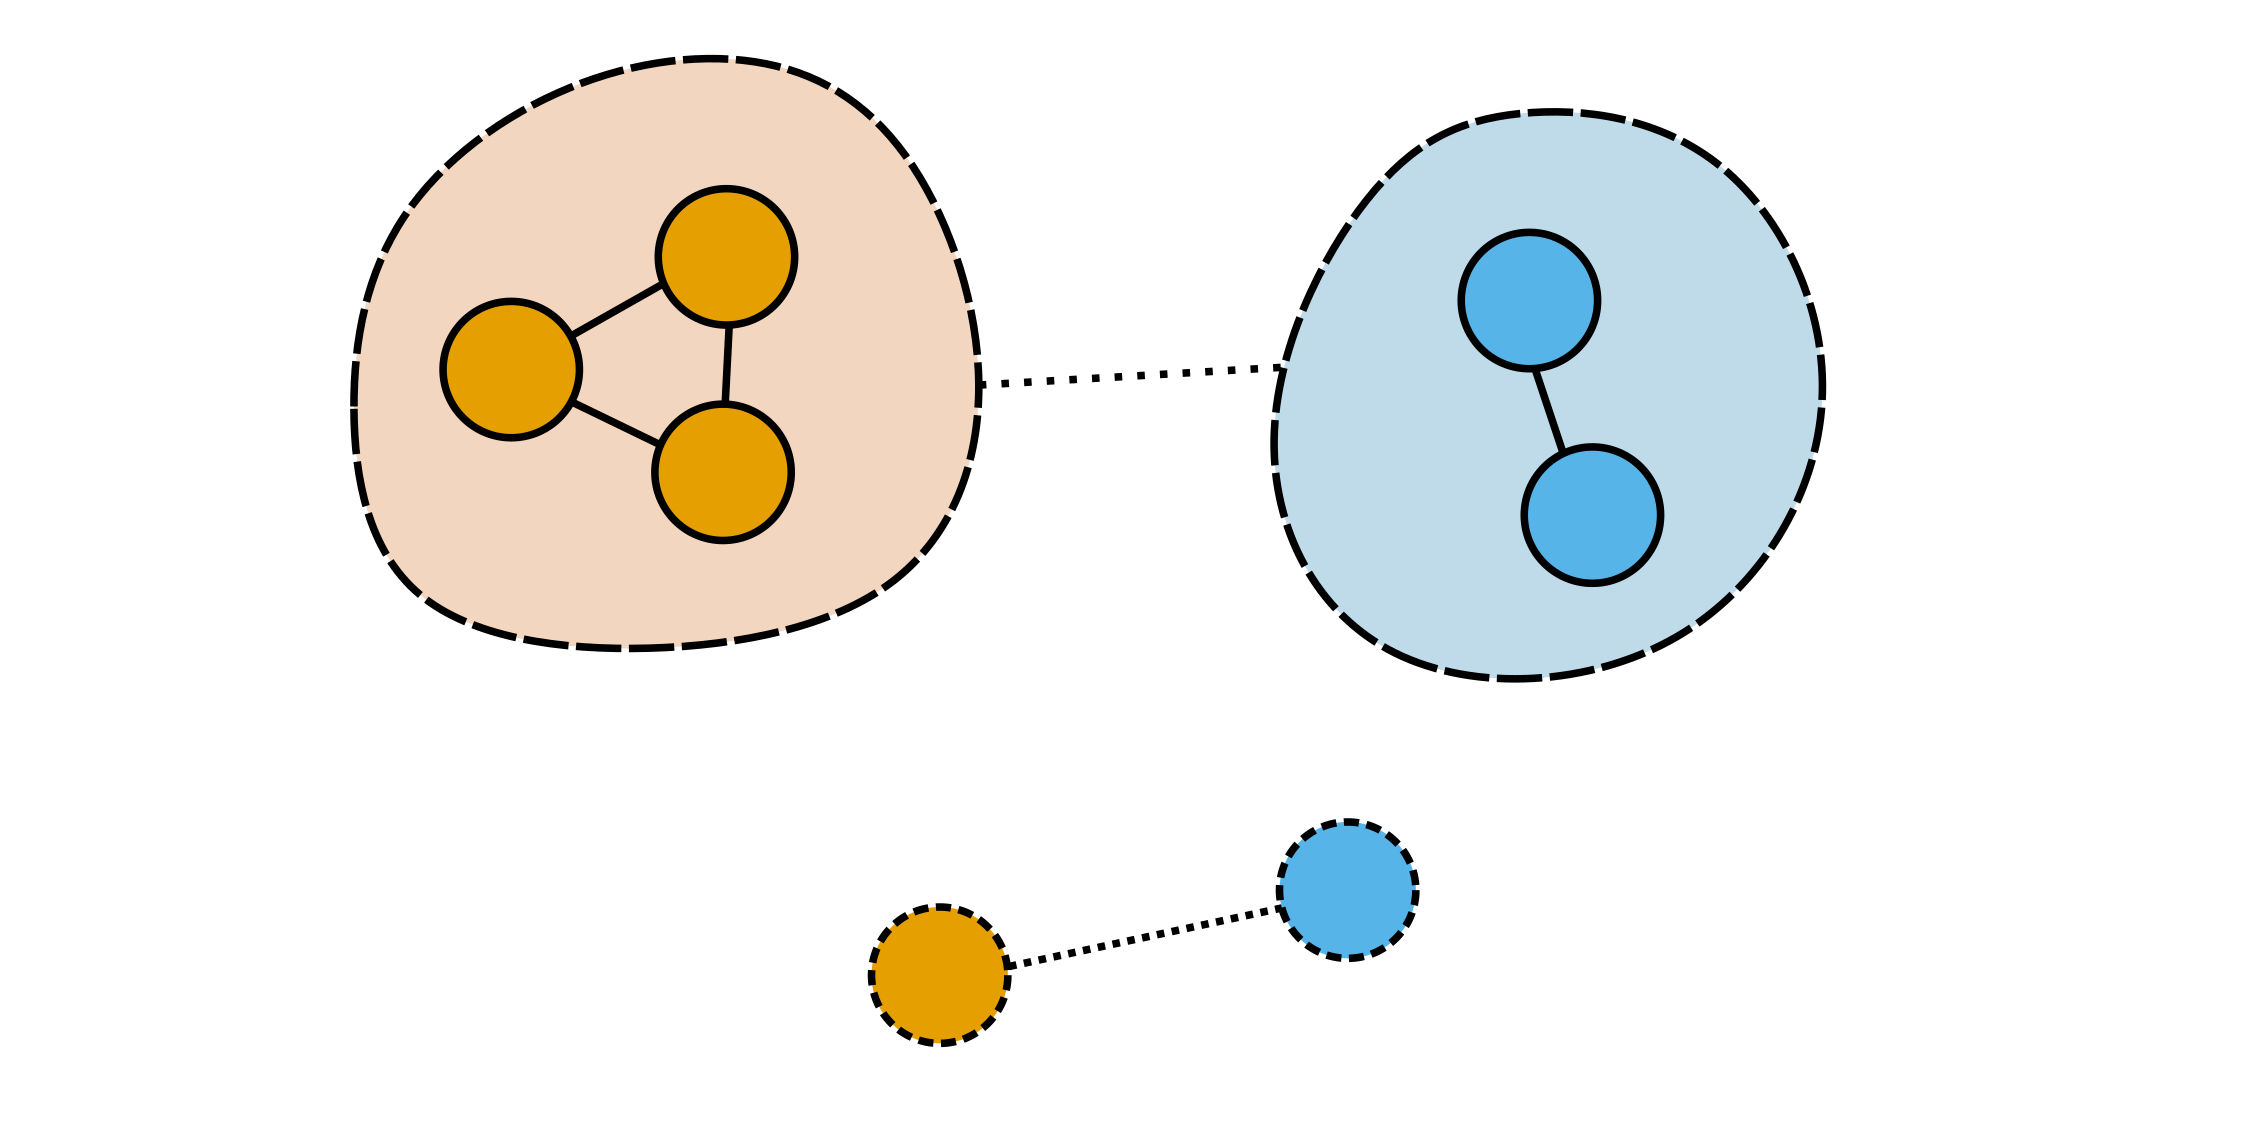
\includegraphics[width=\textwidth]{Figure 16.3.C}
\caption{The five microstates can be abstracted as two macrostates as if they formed a reducible Markov chain}
\end{figure}
\noindent % 12 states
We say that the solid lines indicate states that communicate strongly and dotted lines indicates that they communicate weakly. The dashed lines around a cluster is an abstraction of a larger state that is porous.

For a transition matrix $P$, we can abstractly represent the communication classes by separating the matrix into blocks. The diagonals blocks represent communication classes, and the non-diagonal blocks represent transitions between classes:
\[P^\tau = 
\left[ \begin{array}{c c|c c c}
\frac{1}{2} & \frac{1}{2} & \varepsilon & \varepsilon & \varepsilon \\[2pt]
\frac{1}{2} & \frac{1}{2} & \varepsilon & \varepsilon & \varepsilon \\[2pt]
\hline \\[-2.3ex]
\varepsilon & \varepsilon & \frac{1}{3} & \frac{1}{3} & \frac{1}{3} \\[2pt]
\varepsilon & \varepsilon & \frac{1}{3} & \frac{1}{3} & \frac{1}{3} \\[2pt]
\varepsilon & \varepsilon & \frac{1}{3} & \frac{1}{3} & \frac{1}{3}
\end{array} \right]
\rightarrow
P^\tau = 
\left[ \begin{array}{c|c}
P_1 & \varepsilon \\
\hline
\varepsilon & P_2
\end{array} \right]
\]
In this example, the determinant within each class is approximately $0$ some finite time $\tau$. The communication strength between classes is some infinitesimal transition probability $\varepsilon$. What we want to say about what defines a class is that the determinant of the matrix in each partition is approximately $0$ after some finite amount of time.


\chapter{Class Stochastic Matrices}
A \index{class stochastic matrix}\textbf{class stochastic matrix} is a stochastic matrix $Q_{m \times m}$, and it is the dimensionality reduction of stochastic matrix $P_{n \times n}$ at time $t$ such that:
$$Q = K^+ P^t K$$
We define $K$ as the classification matrix of size $n \times m$ and $K^+$ as the Moore-Penrose pseudo-inverse of $K$ of size $m \times n$. We may disambiguate $P$ as the state transition matrix or state stochastic matrix.

A \index{classification matrix}\textbf{classification matrix} $K$ is a right-stochastic matrix that compresses the $n$ prime states of the stochastic matrix $P^t$ into $m$ composite states of the stochastic matrix $Q$. The classification matrix $K$ is a $(n \rightarrow m)$ projection of the state probability vector $y_{1 \times n}$. We may therefore define the class probability vector as $y K$. We may call $K^+$ the decompression matrix.\footnote{It is not accurate to call $K^+$ the declassification matrix. It inexactly separates each class into its component states, but information is irreversibly lost when passing through $K$ akin to information entering a black hole.} An optimal compression retains the $m$ largest eigenvalues of $\Lambda^t = \{\lambda_1^t,...,\lambda_n^t\}$. Non-optimal compression does not retain these slowly decaying eigenvalues.

In terms of machine intelligence, the optimal compression of a dynamical system uses the longest lasting eigenvalues because it will minimize the divergence of predictions in the state space over time. In contrast, the superfluous information contained in fast decaying eigenvalues is washed away with few time steps. Optimal compression must use the largest eigenvalues to minimize the cumulative prediction error, and they do so for \textit{any} error metric.

The name class stochastic matrix is important. The stochastic matrix of a random walk eventually converges onto a uniform distribution, but it first converges to be approximately uniform within each diffusion class. Similar to how a reducible Markov chain has multiple communication classes, a class stochastic matrix has multiple classes that weakly communicate \textit{between} classes and strongly communicate \textit{within} classes. We also adapt statistical classification algorithms to classify rows of $P^t$.

The following state transition matrix $P$ has an obvious class structure as a block diagonal matrix:
\[P= 
\left[\begin{array}{c c|c c c}
\frac{1}{2} & \frac{1}{2} & 0 & 0 & 0 \\[2pt]
\frac{1}{2} & \frac{1}{2} & 0 & 0 & 0 \\[2pt]
\hline \\[-2.3ex]
0 & 0 & \frac{1}{3} & \frac{1}{3} & \frac{1}{3} \\[2pt]
0 & 0 & \frac{1}{3} & \frac{1}{3} & \frac{1}{3} \\[2pt]
0 & 0 & \frac{1}{3} & \frac{1}{3} & \frac{1}{3}
\end{array}\right]\]
We introduce a small jump probability $\varepsilon$, and this $\varepsilon$ represents a small, finite value in which the prime states in a composite state weakly communicate with prime states from another composite state. 

Here is the corresponding graph visualization of $P$ if we introduce the jump probability $\varepsilon$:
\begin{figure}[H]
\centering
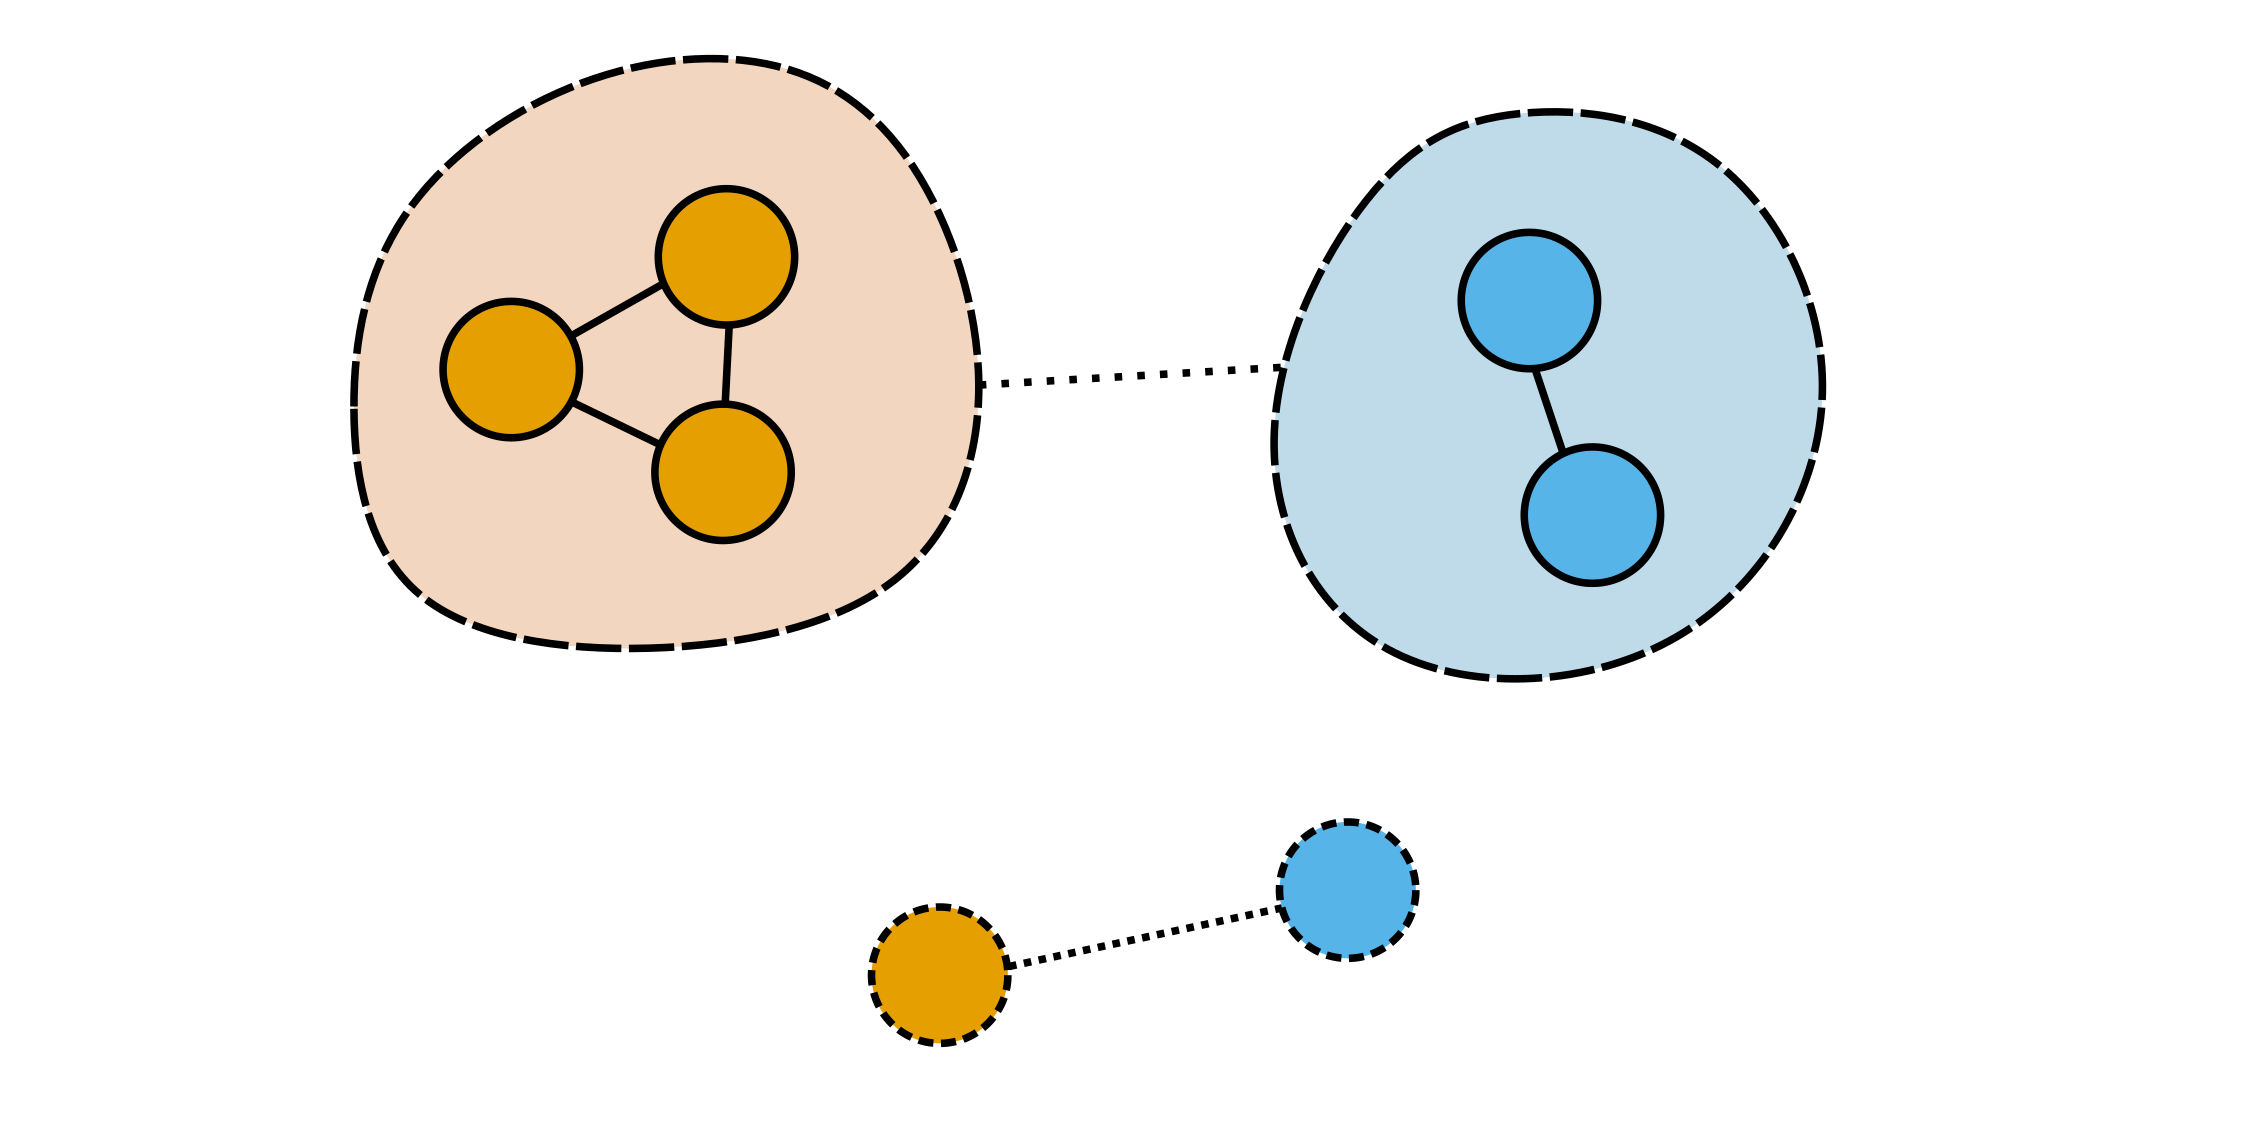
\includegraphics[width=\textwidth]{Figure 16.3.C}
\caption{Each state in a class $i$ has a $1-\varepsilon$ chance of moving to a state within class and a $\varepsilon$ chance of traveling to a state in any other class}
\end{figure}
\noindent % Graph of the communication classes.
The communication gap between two classes is large and within each class is small. We use this jump probability to define a new transition matrix $P^*$.

We now define our new transition matrix $P^*$ with class exit probability $\varepsilon$ distributed uniformly among states outside of a given class:
\[P^*= 
\left[\begin{array}{c c|c c c}
\frac{1}{2}-\frac{\varepsilon}{2} & \frac{1}{2}-\frac{\varepsilon}{2} & \frac{\varepsilon}{3} & \frac{\varepsilon}{3} & \frac{\varepsilon}{3} \\[2pt]
\frac{1}{2}-\frac{\varepsilon}{2} & \frac{1}{2}-\frac{\varepsilon}{2} & \frac{\varepsilon}{3} & \frac{\varepsilon}{3} & \frac{\varepsilon}{3} \\[2pt]
\hline \\[-2.3ex]
\frac{\varepsilon}{2} & \frac{\varepsilon}{2} & \frac{1}{3}-\frac{\varepsilon}{3} & \frac{1}{3}-\frac{\varepsilon}{3} & \frac{1}{3}-\frac{\varepsilon}{3} \\[2pt]
\frac{\varepsilon}{2} & \frac{\varepsilon}{2} & \frac{1}{3}-\frac{\varepsilon}{3} & \frac{1}{3}-\frac{\varepsilon}{3} & \frac{1}{3}-\frac{\varepsilon}{3} \\[2pt]
\frac{\varepsilon}{2} & \frac{\varepsilon}{2} & \frac{1}{3}-\frac{\varepsilon}{3} & \frac{1}{3}-\frac{\varepsilon}{3} & \frac{1}{3}-\frac{\varepsilon}{3}
\end{array}\right]\]
Because the weakly communicating transition matrix an eigenvalue $\lambda_1 = 1$ with uniform eigenvector $\phi_1 = \frac{1}{n}$, all rows of the transition matrix converge to the vector $\frac{1}{n}$ as $t \rightarrow \infty$. In the transition matrix with separate communication classes, each class has their own eigenvector corresponding to the uniform distribution within the communication class.

Using our informal intuition and no formal algorithm, we may judge the stochastic matrix $P$ to have the following hard classification matrix $K$:
$$K =
\begin{bmatrix}
1 & 0 \\
1 & 0 \\
0 & 1 \\
0 & 1 \\
0 & 1
\end{bmatrix}$$
A key property of hard classification matrices is that $K^+ K$ is precisely the stochastic matrix with $m$ communication classes that are uniformly distributed within each class
\[K^+ K = 
\left[\begin{array}{c c|c c c}
\frac{1}{2} & \frac{1}{2} & 0 & 0 & 0 \\[2pt]
\frac{1}{2} & \frac{1}{2} & 0 & 0 & 0 \\[2pt]
\hline \\[-2.3ex]
0 & 0 & \frac{1}{3} & \frac{1}{3} & \frac{1}{3} \\[2pt]
0 & 0 & \frac{1}{3} & \frac{1}{3} & \frac{1}{3} \\[2pt]
0 & 0 & \frac{1}{3} & \frac{1}{3} & \frac{1}{3}
\end{array}\right]\]
We have thus reconstructed the block diagonal matrix from earlier.

Let us suppose that we wish to perform a similar example for a much larger class matrix with the following visualization:
\begin{figure}[H]
\centering
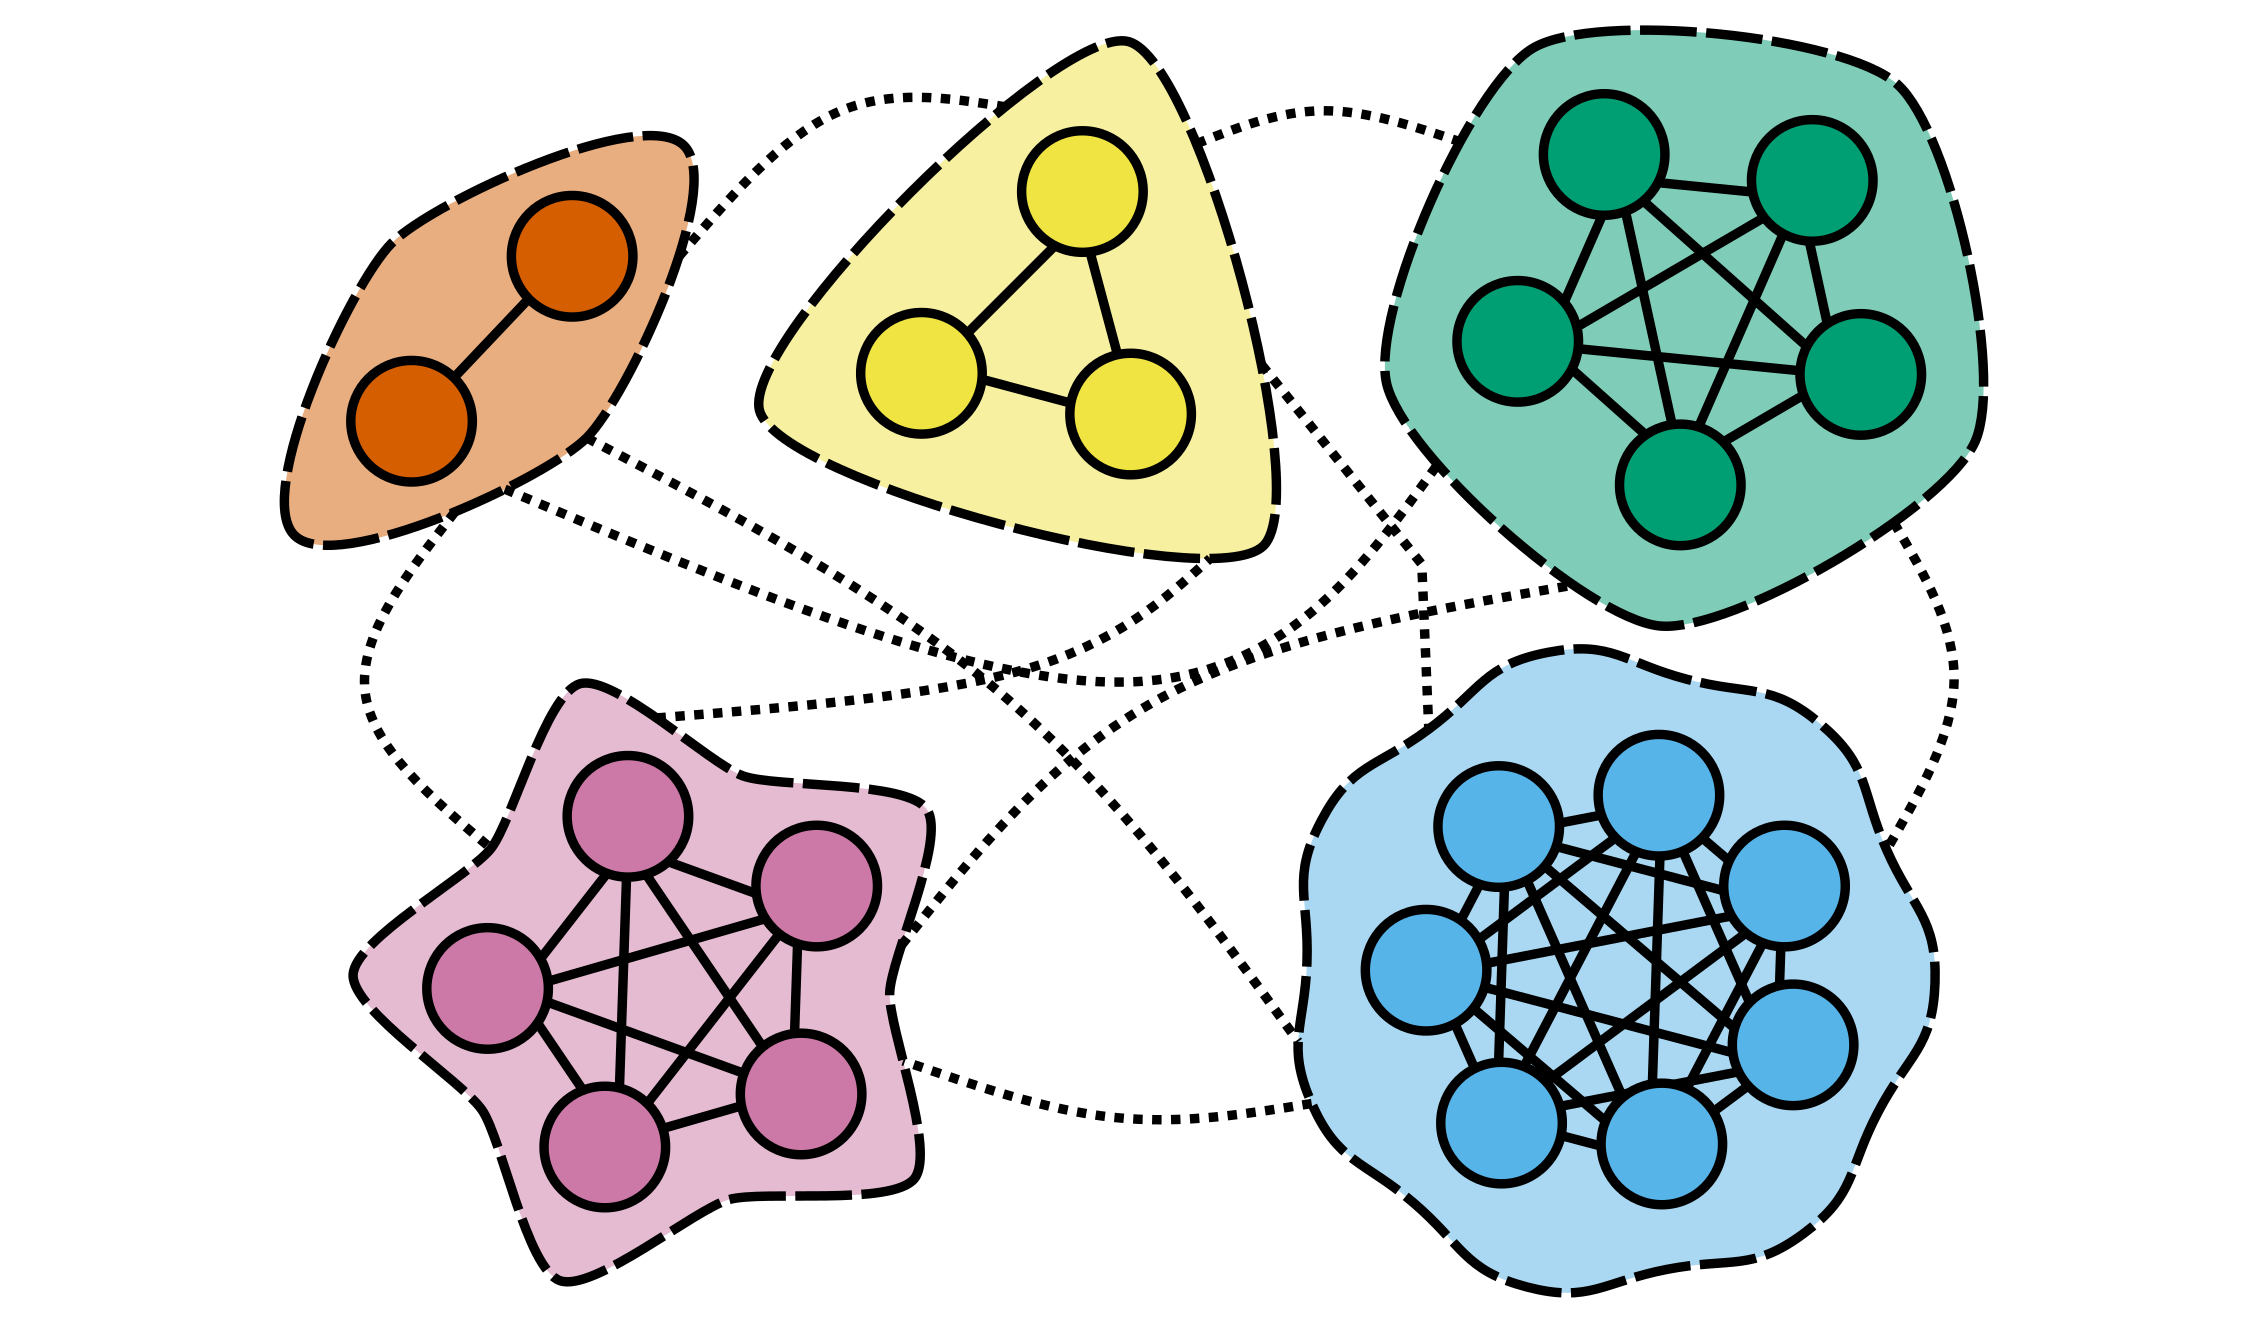
\includegraphics[width=\textwidth]{Figure 16.4.A}
\caption{A system with $22$ states in $5$ classes that weakly communicate}
\end{figure}
\noindent
Each state in a class $i$ has a $1-\varepsilon$ chance of moving to any state within its class and a $\varepsilon$ chance of traveling to a state in any other class. The ``obvious'' class structure means that we can define the classification matrix $K$ intuitively and without an algorithm.

Let us suppose for the example that we want the class stochastic matrix $Q$ at time $t = 20$. We calculate $Q$ using the formula $Q = K^+ P^{20} K$. According to the class estimation formula:
$$k(t) = \frac{n^2}{\sum \Theta(t)}$$
the estimated number of classes is $m = \lceil k(20) \rceil = 5$. If we use any other classification matrix $K$, we lose the property that $Q$ possesses the $m$ largest magnitude eigenvalues of $P^{20}$. In this example, the computed eigenvalues of $P^{20}$ are:
\begin{quote} 1.000000e+00, 9.569909e-01, 9.569858e-01, 9.569792e-01, 9.569739e-01, 1.987494e-307, 3.814810e-314 \end{quote} 
Likewise, the computed eigenvalues of $Q$ are 
\begin{quote} 1.0000000, 0.9569909, 0.9569858, 0.9569792, 0.9569739 \end{quote} 
It may perhaps seem ``obvious'' that such a toy example that $Q$ preserves the $m$ largest eigenvalues of $P^{20}$, but it is not so obvious that it should be the case for transition matrices in general.

There are two kinds of classification matrices $K$: hard classification and soft classification. A hard classification matrix $K$ may only allow Boolean values $\mathbb B_\circ = \{0 , 1\}$. In contrast, a soft classification matrix $K$ may allow any value from the set $[0, 1]$ as long so the row sums to $1$. A hard classification matrix is preferable to a soft classification matrix because a microstate should completely diffuse across its macrostate before two macrostates are ready to merge. Any precision gained by using a soft classification matrix is lost if a microstate is uniformly distributed within its class in due time. Hard classification is essentially a function of human language, meaning that words are required to decompress a general sentence into more detail. Language structure depends upon a latent contraction hierarchy.


The intuitionist justification for hard classification is that the \index{partial determinant}\textbf{partial determinant} of $P^t$ for some $(i,j)$ is approximately $0$ if these state belong in the same class:
$$\begin{vmatrix}
(P^t)_{(i, i)} & (P^t)_{(i, j)} \\ 
(P^t)_{(j, i)} & (P^t)_{(j, j)} 
\end{vmatrix} \approx 0 $$
The diagonal entries represent self-flow and the off-diagonal entries represent cross-flow. States in the same class continuously flow and diffuse between each other until they are indistinguishable.

The name of classification matrix is also appropriate because of the hierarchical tree structure similar to taxonomy, the science of classification:
\begin{figure}[H]
\centering
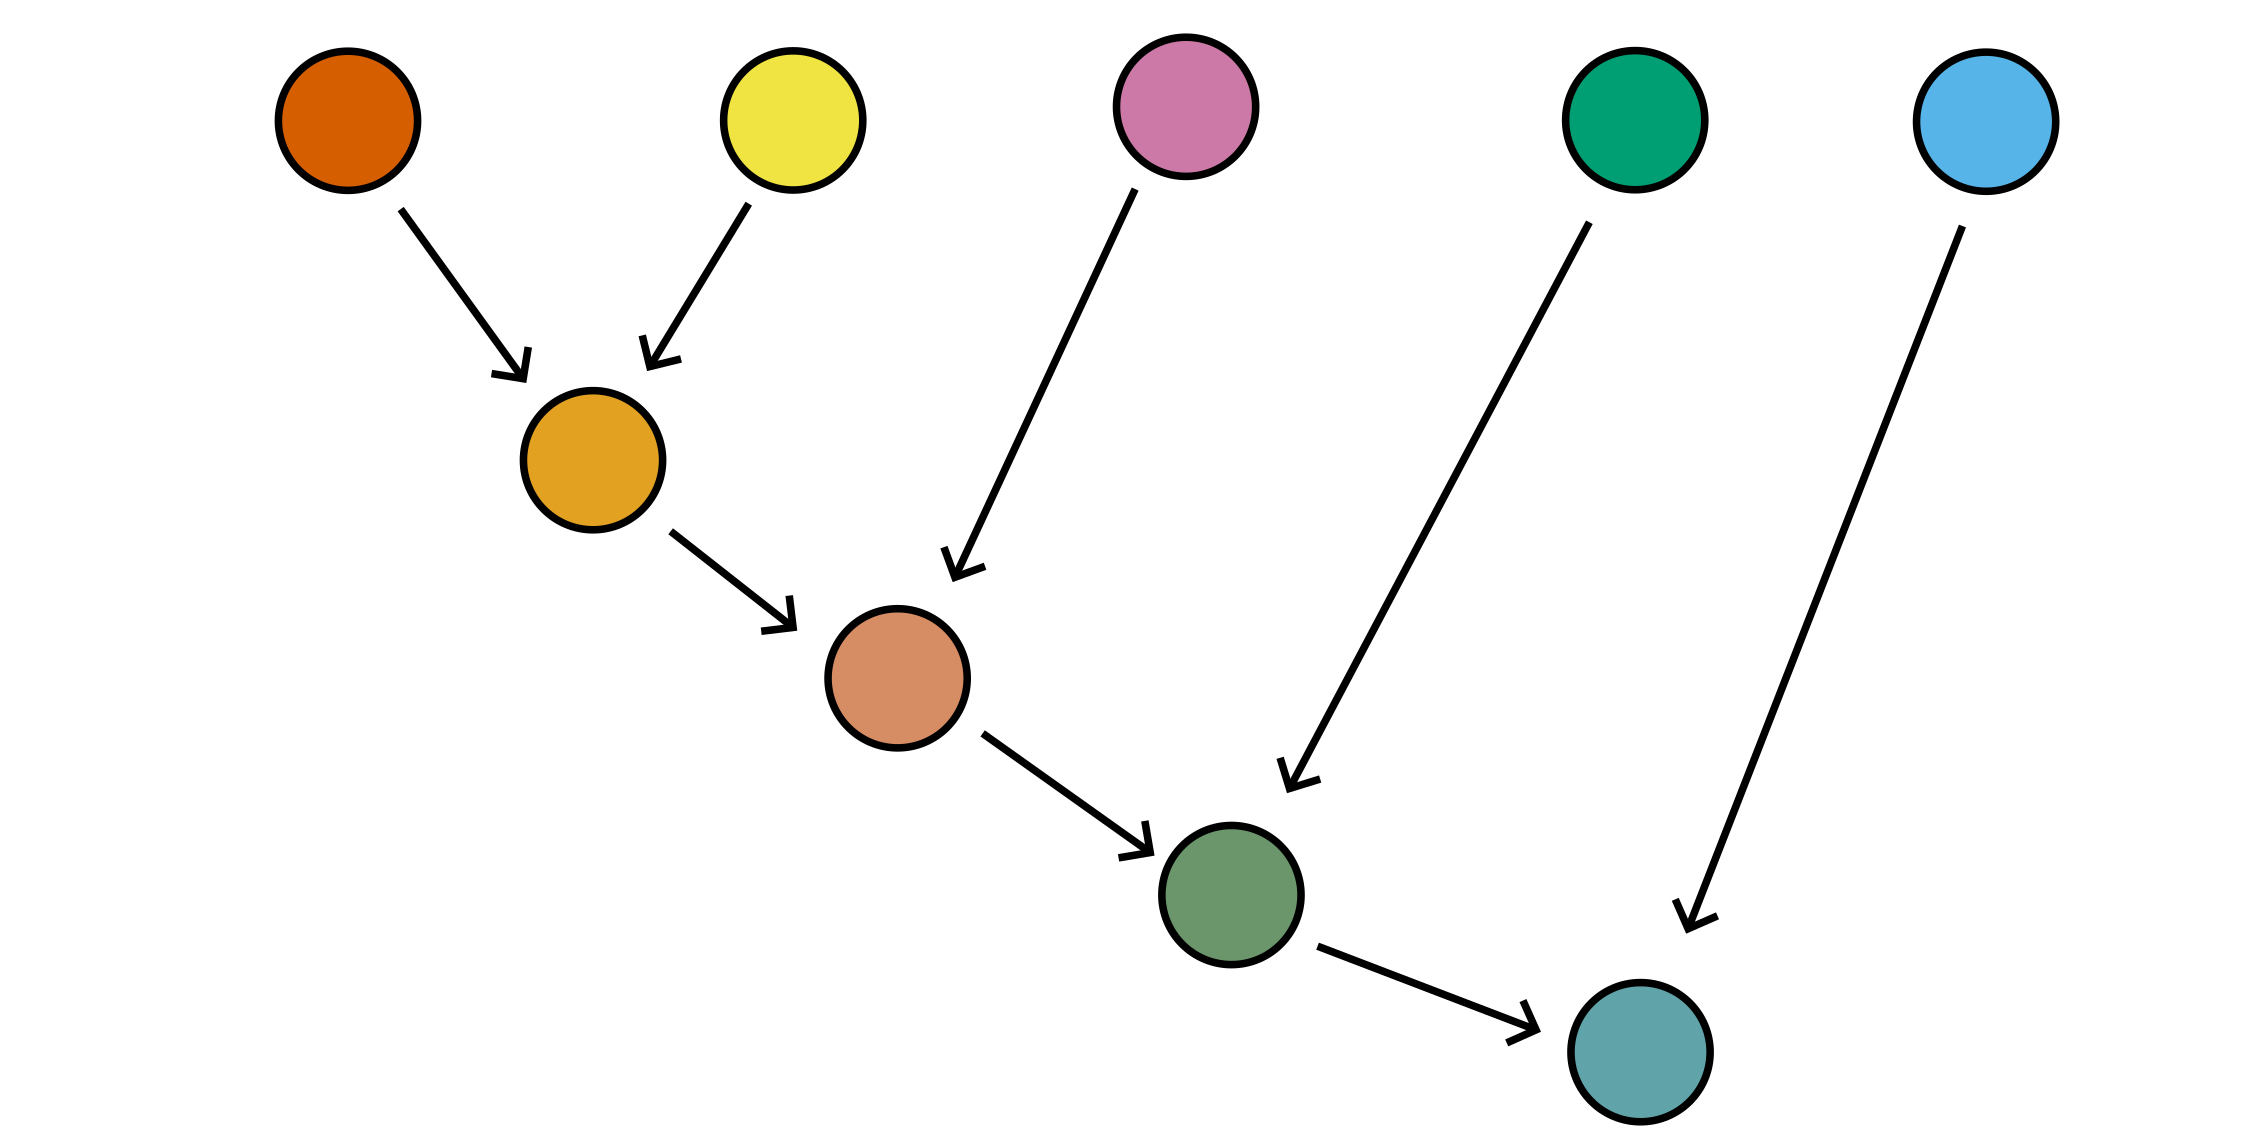
\includegraphics[width=\textwidth]{Figure 16.4.B}
\caption{A class merges all microstates into a single macrostate}
\end{figure}
\noindent % A comparison of scientific taxonomy and a state space hierarchy
A scientific taxonomy starts with a general class and splits into a greater number of specific classes. In contrast, a contraction hierarchy of the state space $\mathcal X$ starts with specific classes and merges into fewer number of general classes.

This begs the question: What algorithm determines the optimal classification structure matrix $K$ that results in $Q$ having the $m$ largest eigenvalues of $P^t$? There are a few methods I recommend:
\begin{enumerate}
\item $k$-means Clustering
\item $k$-means by Correlation
\item Correlation Merge
\end{enumerate}
Many programming languages have $k$-means clustering available as a coding package. My $k$-means by correlation algorithm is an adaptation of $k$-means that leverages the triangular structure of the simplex, balancing speed and accuracy. Correlation merge is deterministic and slow in finding the global optima, but its cardinal sins are being obvious, boring, and uncreative.

The \textbf{$\boldsymbol{k}$-means clustering}\index{k-means clustering} algorithm is a classification algorithm that assigns data points to a class depending upon their distance to a class average.
\begin{enumerate}
\item Initialize $k$ points to be the center of a class.
\item Assign a class each point depending on the nearest class center by Euclidean distance.
\item Calculate the new center of each class by the average value of assigned members.
\item Iterate until convergence or until maximum iterations have run.
\end{enumerate}
This algorithm works reasonably well for classifying correlated rows of a transition matrix $P$. However, it may fail to converge to the optimal cluster for any given data set depending on how the $k$ points are initialized. It implicitly minimizes the sum of square distances within each class, and the problem of minimizing overall sum of squares is \textbf{NP}-hard computational complexity. Thanks to support from mathematics academia, $k$-means is available as a package in common coding languages.

The \textbf{$\boldsymbol{k}$-means by correlation}\index{k-means by correlation} algorithm is a classification algorithm that assigns data points to a class depending upon their correlation to a class expectation. Since we know that the rows of a transition matrix $P^t$ are bound to the $(n-1)$-simplex for $t \in \mathbb N$, correlation best exploits the triangular structure.
\begin{enumerate}
\item Initialize $k$ points to be the center of a class.
\item Assign a class each point depending on the nearest class center by correlation.
\item Calculate the new center of each class by the average value of assigned members.
\item Iterate until convergence or until maximum iterations have run.
\end{enumerate}
Notice the similarity to $k$-means clustering. It may likewise fail to converge to the optimal class assignment, and the primary issue is accidentally merging two classes and forcing one empty class. Trials of the algorithm on the Markov chain represented in \textit{Figure D.2} often merges the smallest classes but almost never the large class.

This can be easily circumvented by doubling the amount of possible classes to $2k$, then cutting the algorithm runtime shortly after we count $k$ non-empty classes.\footnote{We may try $k^2$ or $2^k$ classes so long as they are less than the number of original points $n$, but it is unnecessary.} This finite runtime after reaching $k$ classes is called the refinement period, we repair empty classes by randomly generating a new point within the simplex.\footnote{The refinement period gives us a finite history to check repairs usurping classes. If our repair vector lands inside of an established class, the class will split in two. The algorithm will push one of the redundant vectors out.} I call these modifications of doubling, counting, refining, and repairing to create the ``shotgun method'' for $k$-means by correlation. We discard all empty classes when constructing the classification matrix $K$. This is rather easy to code, maintaining the speed of $k$-means while being almost as accurate as correlation merge.

Merging rows by correlation, or \textbf{correlation merge}\index{correlation merge} is likely the best deterministic method since the intuition is that classes are defined by correlation. Expect it to be rather slow however. There are a few different ways that we can merge rows of $P^t$:
\begin{enumerate}
\item Merge rows if all of their mutual correlations is greater than some constant.
\item Merge rows if any two have a mutual correlation greater than some constant.
\item Merge rows by strongest correlations until we reach $m$ classes.
\end{enumerate}
We defined the matrix $\Theta(t)$ as the cosine similarity between between the $i$-th and $j$-th row of $P^t$, and we defined:
$$m = \bigg \lceil \frac{n^2}{\sum \Theta(t)} \bigg \rceil$$
as the estimated number of classes. Triangle inequality is how we justified the dimensionality reduction of $n$ states to $m$ classes in the first place. If two points $A, B$ share an implied class center $C$, then triangle inequality places good bounds on how dissimilar $A$ and $B$ can be if each is highly correlated with $C$.

The covariance matrix $\Sigma$ for a population sample $X_1,...,X_n$ may be used to derive the correlation $\theta$ between any element $X_i$ and its sample average $\bar X$:
$$\theta(X_i, \bar X) = \frac{\mathrm{E}[\Sigma_{(i, \cdot)}]}{\textnormal{trace}(\Sigma_{(i, \cdot)})}$$
Recall that each row of a transition matrix $P$ is a unit magnitude vector that defines the correlation between input state $i$ at time $0$ and output state $j$ at time $t$, and recall that $\Theta(t)$ defines the correlation in distribution between row $i$ and row $j$ of $P^t$. We may simplify the correlation as the average of the correlation matrix $\Theta$:
$$\theta(X_i, \bar X) = \mathrm{E}[\Theta_{(i, \cdot)}]$$
We may also generally say that the correlation between any state $i$ and another class $C$ is the average of class elements $j \in C$ in the $i$-th row of the correlation matrix $\Theta$:
$$\theta(X_i, \bar X_C) = \mathrm{E}[\Theta_{(i, j \in C)}]$$
We call this the \textbf{eigenclass correlation theorem}\index{eigenclass correlation theorem}, and it states the correlation between a row in transition matrix $P_i$ and a set of states $j \in C$ is precisely the average correlation between the $i$-th row and rows $j \in C$. 

Here is the proof of the statement in non-matrix form. The correlation $\theta$ between sample component $X_i$ and sample average $\bar X$:
$$\theta (X_i, \bar X) = \frac{X_i \cdot \bar X}{|X_i| |\bar X|}$$
We split our correlation into a summation of $n$ terms with weight $\frac{1}{n}$:
$$ \frac{X_i \cdot \bar X}{|X_i| |\bar X|}  = \frac{1}{n} \sum\limits_{j=1}^n \frac{X_i \cdot \bar X}{|X_i| |\bar X|}$$
Notice our average $\bar X$ can be split in the summation into its original components $X_j$:
$$\frac{1}{n} \sum\limits_{j=1}^n \frac{X_i \cdot \bar X}{|X_i| |\bar X|} = \frac{1}{n} \sum\limits_{j=1}^n \frac{X_i \cdot X_j}{|X_i| |\bar X|}$$
Since our data components have the same magnitude $|X_i| = |X|$ for any $i$, this means that $|\bar X| = |X|$. We may simplify:
$$\frac{1}{n} \sum\limits_{j=1}^n \frac{X_i \cdot X_j}{|X|^2} = \frac{1}{n} \sum\limits_{j=1}^n \Theta_{(i, j)}$$
Therefore, the correlation of unit magnitude elements is given by:
$$\theta (X_i, \bar X) = \mathrm{E}[\Theta_{(i, \cdot)}]$$
We may therefore generalize this correlation to subsets $C \subset \mathcal X$ such that:
$$\theta(X_i, \bar X_C) = E[\Theta_{(i, j \in C)}]$$
defines the correlation between a state $X_i$ and the subset $C$, regardless of whether $X_i$ is or is not in $C$.

For an intuition about the eigenclass correlation theorem, suppose we have three unit-magnitude one-dimensional vectors $X_1 = +1$, $X_2 = +1$, and $X_3 = -1$. The correlation between $X$ and the class average $C = (X_1 + X_2 + X_3) / 3$ equals the average of correlation between $X_1$ and the components of $C$. Due to triangle inequality, classifications defined by correlation to some latent class vector $C$ means the dissimilarity of any two class elements is bounded by some constant $\varepsilon_C$. The maximum dissimilarity constant may differ between classes.

Some worthwhile research directions are whether or not the maximal interlink vertex (MIV) between two classes are always adjacent to each other. Here is the problem statement:
\begin{quote}
MIV($A$, $B$) is the element of class $A$ is the element of class $A$ with the highest correlation to class $B$. 

MIV($B$, $A$) is the element of class $B$ is the element of class $B$ with the highest correlation to class $A$. 

Are MIV($A$, $B$) and MIV($B$, $A$) always adjacent?
\end{quote}
The practical application of this question is speeding up the search for a shortest path. The assumption is that these vertices in each class that maximize the cross correlation are the optimal boundary of each class.

AI corporation rely on fear, uncertainty, and doubt (FUD) to monopolize the attention economy. Without a firm theoretical understanding of class stochastic matrices, artificial intelligence models will continue to fall short of the promise of practical application. While I continue my work alone, I hope my ideas inspire more independent researchers to disbelieve the hype and work diligently to improve computer vision, autonomous control systems, and computer graphics. 

State spaces of a finite stochastic matrix are often so large that we are working with measurable functions of states instead of the state space graph itself. This means that an artificial intelligence agent or human necessarily struggles when similarity in measure $\mu_i \sim \mu_j$ is not biconditional with similarity in probability distribution $p_i \sim p_j$. It is necessary to find an encoding measure $\mu^\prime$ of the direct measure $\mu$ such that:
$$\mu^\prime_i \sim \mu^\prime_j \iff p_i \sim p_j$$
in order to properly predict dynamical systems.


\chapter{Random Backtrack Algorithm}
The \textbf{random backtrack}\index{random backtrack} algorithm is a way to use parallel computing to speed up the calculation of a Boolean random walk transition using the minority class of particles versus antiparticles. In general, there is no fast parallel computation algorithm for maximum independent sets (MIS) due needing a way to handle ``collisions''. The (hyper)edge coloring of a Boolean random walk is $2$, and the coloring is known. Therefore, we may accelerate our MIS algorithm using the smaller of $k$ particles or $N-k$ antiparticles as the starting point for our algorithm.

Each Boolean cell has a unique index and neighbors stay the same, therefore we can rely on walking to a neighbor as being assigned an index in a chain. The \textit{simple random backtrack algorithm} is as follows:
\begin{enumerate}
\item Perform the first random walk from each cell from minority class, not considering the validity of the finite difference
\item Record if the first walk traversed to a majority class cell or a minority class cell
\item Perform the second random walk from the new cell, not considering the validity of the finite difference
\item If the second random walk returned to the original cell \textbf{AND} the first traversal was of majority class, lock the switch
\item Invalidate all switches pertaining to each locked cell
\item Loop prior steps for unpaired cells until we obtain our maximal independent set
\end{enumerate}
This random backtrack algorithm performs a random walk from each minority class, then it checks if it is a valid Boolean random walk. However, this algorithm has the problem of wasting compute by having the starting minority class cell sometimes walking to another minority class cell, creating a invalid transition. We can recover this wasted computation time in a way that preserves the probability distribution for the selection of the MIS.

An alternative characterization of the random backtrack algorithm uses more memory in exchange for wasting less time, and this memory is used to preprocess a lookup table. The \textit{indexed random backtrack algorithm} is as follows:
\begin{enumerate}
\item Random sample a single valid forward or backward differences for all minority class origins 
\item Random sample a single valid forward or backward differences for all majority class neighbors 
\item Initialize a vector of indices $v_0$ as containing each minority class index
\item Traverse to the previously sampled index of the minority class to the majority class
\item Define the vector of indices $v_1$ as containing each majority class index from the previous step
\item Traverse to the previously sampled index majority class to the minority class
\item Define the vector of indices $v_2$ as containing each minority class index from the previous step
\item Compare vectors $v_0$ and $v_2$. If returned to origin, lock the traversal as mutual partners
\item Invalidate all switches pertaining to each locked cell
\item Loop prior steps for unpaired cells until we obtain our maximal independent set
\end{enumerate}
This dramatically speeds up a linear time algorithm $O(n)$ for sampling a some finite order to a logarithmic time algorithm $O(log(n))$ due to backtrack depending on pairing mutual sides from the face of a cube. There are also zero collisions to worry about since we sampled the majority class's orientation ahead of time. The oversampling of transitions from the majority class is constrained by our first traversal.

An exact scaling of simple random backtrack algorithm is given by the formula: 
$$O(-\log_{(2d)^2}(n))$$
In other words, random backtrack works much faster when there are more than $(2d)^2$ leftover Boolean cells of the minority class. If there are less than $(2d)^2$ leftover Boolean cells of the minority class, it is better to switch to the standard $O(n)$ time algorithm. The standard $O(n)$ is random, but it always creates a single pair after each cycle.

For the indexed random backtrack algorithm, it depends on the average degree of each vertex squared $\mathrm{E}[\textnormal{deg}(V)]^2$ of a given graph, but it is a good rule of thumb to say it is still $O(-\log_{(2d)^2}(n))$. Indexing is slightly faster and more efficient, but I still recommend switching to the $O(1)$ algorithm when $<(2d)^2$ unpaired Boolean cells remain.


\chapter{Specification of Classes}
In many languages, blue and green shared the same word early in the language's life cycle. When humans needed to distinguish between blue and green, a new word would appear. This textbook also takes great care to use the Okabe-Ito colorblind palette to help readers with colorblindness distinguish diagrams. Even though colorblind individuals have all red, green, and blue light receptors, the neural pathways do not distinguish these signals. The disadvantage is to distinguishing less colors compared to a trichromatic individual, but the advantage is the reduced computational power needed to process a dichromatic or monochromatic world.

Let $\pi_Q$ be the stationary distribution of class transition matrix $Q$, and let $\pi_P$ be the stationary distribution of state transition matrix $P$. Then the stationary distribution of $Q$ is given by:
$$\pi_Q = \pi_P \cdot K$$
in which $K$ is the hard classification matrix $K$. This means $K$ allocates the stationary distribution probabilities in a way that preserves the original mass of class elements. A strange implication is that:
$$\implies \pi_P \approx \pi_Q \cdot K^+$$
This leads us to the inverse problem of classification: specification.\footnote{An alternative word for specification is declassification or deconception.}

Calculating $Q$ by classifying the rows of $P^t$ is arbitrarily easy using the $k$-means by correlation algorithm, but determining $P$ from $Q^{1/t}$ is difficult. Splitting $Q$ until we get $P$ is difficult because classes are defined by class elements being computational indistinguishable over longer time periods. This is the fundamental problem of having a sensor with a low sampling rate.

Imagine seeing the world through a narrow tube. You have essentially reduced the state space that your eyes can work with. Outside of this narrow vision, it is difficult to make predictions. Insects resolve this problem using compound eyes, the equivalent of having many narrow tubes. A sensor's state space can only making determinations using a subset of the state space. A sensor by definition only accesses a subset of the state space.

This is a problem for physics. The sensors that are available interact only with the reduced state space $\mathcal S$ instead of the complete state space $\mathcal X$. If the method by wish to specify $Q$ into $P$ uses a subset of the system $X$, then you can only make predictions using the sensor region $S \subset X$. The reduced state space $\mathcal S$ must apply the rule of unconditional probability to each cell $x$ not in the sensor $S$. Therefore, the sensor cannot classify states using out-of-bound points $x \notin S$. Having a multitude of points can help, but this is a fundamental restriction.

The solution that natural biology has come up with is multi-modal sensors: eyes, ears, nose, mouth, skin. By diversifying your sensors, you interact with a dramatically larger portion of the state space. The gain in predictive power can be greater than having duplicate sensors. A similar object or deceiving object has many more layers of sensors that it has to fool in order to be indistinguishable in the reduced state space $\mathcal S$.
 
In general, having more sensors, having more frequent sensor samples, and having more diverse sensors will better approximate the complete state space $\mathcal X$.

\backmatter

\printindex

\end{document}